\chapter{ಆಡಳಿತ ವ್ಯವಸ್ಥೆ}

ಜಿಲ್ಲೆಯಲ್ಲಿರುವ ಶಾಸನಗಳ ಆಧಾರದ ಮೇಲೆ ರಾಜಮನೆತನಗಳ ಆಡಳಿತ ಪದ್ಧತಿಯನ್ನು ಅಥವ ವ್ಯವಸ್ಥೆಯನ್ನು ನಿರೂಪಿಸಲಾಗಿದೆ. ಜೊತೆಗೆ ಈ ಆಡಳಿತ ವ್ಯವಸ್ಥೆಯ ಅಂಗವಾಗಿದ್ದ ಮಹಾಪ್ರಧಾನ ದಂಡನಾಯಕರಿಂದ ಹಿಡಿದು ವಿವಿಧ ಮಟ್ಟದ ಅಧಿಕಾರಿಗಳು ಮತ್ತು ಸ್ಥಳೀಯ ಆಡಳಿತದ ಮುಖ್ಯಸ್ಥರಾಗಿದ್ದ ಗಾವುಂಡರುಗಳ ಸಾಧನೆಗಳು, ಅವರ ವಂಶಾವಳಿಗಳನ್ನು ಶಾಸನಗಳ ಆಧಾರದ ಮೇಲೆ ಕಟ್ಟಿಕೊಡಲಾಗಿದೆ. “ಪ್ರಾಚೀನ ಕರ್ನಾಟಕದ ಆಡಳಿತ ವ್ಯವಸ್ಥೆಯನ್ನು ಸ್ಥೂಲವಾಗಿ ಎರಡು ಭಾಗವಾಗಿ ವಿಂಗಡಿಸಬಹುದು. ರಾಜ್ಯಾಡಳಿತ ಮತ್ತು ಊರುಗಳ ಆಡಳಿತ. ಒಂದರ ಸಹಕಾರದಿಂದ ಮತ್ತೊಂದು ನಡೆಯುತ್ತಿತ್ತು”.\endnote{ ಚಿದಾನಂದಮೂರ್ತಿ ಡಾ॥ ಎಂ., ಕನ್ನಡ ಶಾಸನಗಳ ಸಾಂಸ್ಕೃತಿಕ ಅಧ್ಯಯನ, ಪುಟ 321} ಒಟ್ಟಾರೆ ರಾಜ್ಯಾಡಳಿತವನ್ನು ರಾಜ ಹಾಗೂ ಅವನಿಂದ ನೇಮಕ ಮಾಡಲ್ಪಟ್ಟ ಮಹಾಪ್ರಧಾನರೇ ಮೊದಲ್ಗೊಂಡು ಸೇನಬೋವರವರೆಗಿನ ಅಧಿಕಾರಿಗಳು ನೋಡಿಕೊಳ್ಳುತ್ತಿದ್ದರು. ಊರುಗಳ ಅಂದರೆ ಸ್ಥಳೀಯ ಆಡಳಿತವನ್ನು ಗಾವುಂಡರು, ಪ್ರಜೆಗಾವುಂಡರು, ನಾಳ್ಗಾವುಂಡರು ಮೊದಲಾದ ಪರಂಪರಾಗತ ಹಾಗೂ ಅನುವಂಶೀಯ ಸ್ಥಳೀಯ ಆಡಳಿತಗಾರರು ನೋಡಿಕೊಳ್ಳುತ್ತಿದ್ದರು. ಇಬ್ಬರಿಗೂ ರಾಜ್ಯದ ಹಾಗೂ ಪ್ರಜೆಗಳ ಹಿತವೇ ಮುಖ್ಯವಾಗಿತ್ತು.

\section*{ಗಂಗರಕಾಲದ ಆಡಳಿತ ವ್ಯವಸ್ಥೆ}

ಮಂಡ್ಯ ಜಿಲ್ಲೆಯ ಪ್ರದೇಶದಲ್ಲಿ ನಮಗೆ ಮೊದಲಬಾರಿಗೆ ಕಂಡುಬರುವ ಪ್ರಾಚೀನ ಆಡಳಿತ ವ್ಯವಸ್ಥೆ ಎಂದರೆ, ಈ ಪ್ರದೇಶವನ್ನು ದೀರ್ಘ ಕಾಲ ಆಳಿದ ಗಂಗರ ಆಡಳಿತ ವ್ಯವಸ್ಥೆ. ಗಂಗರು ತಮ್ಮನ್ನು ಧರ್ಮಮಹಾಧಿರಾಜರೆಂದು\index{ಧರ್ಮಮಹಾಧಿರಾಜರು} ಹೇಳಿಕೊಂಡಿದ್ದಾರೆ. ಅವರು ಮನುಧರ್ಮಶಾಸ್ತ್ರ ಮತ್ತು ರಾಜನೀತಿಯ ಅನ್ಯಗ್ರಂಥಗಳಿಗೆ ಅನುಗುಣವಾಗಿ ಆಳುತ್ತಿದ್ದರೆಂದು ಶಾಸನಗಳಿಂದ ತಿಳಿದುಬರುತ್ತದೆ.\endnote{ ಸೂರ್ಯನಾಥ ಕಾಮತ್​ ಡಾ॥, ಕರ್ನಾಟಕದ ಸಂಕ್ಷಿಪ್ತ ಇತಿಹಾಸ, ಪುಟ 38} ಹಳ್ಳೆಗೆರೆ ತಾಮ್ರಪಟಗಳಲ್ಲಿ\index{ಹಳ್ಳೆಗೆರೆ ತಾಮ್ರಪಟ} ಮಾಧವನನ್ನು \textbf{“ನೀತಿಶಾಸ್ತ್ರ ವಕ್ತೃ ಪ್ರಯೋಕ್ತೃಕುಶಲೋ”} ಎಂದು, ಶ‍್ರೀ ವಿಕ್ರಮನನ್ನು \textbf{“ಚತುರ್ದ್ಧಶವಿದ್ಯಾಸ್ಥಾನಾಧಿಗಮವಿಮಲಮತಿಃ ನೀತಿಶಾಸ್ತ್ರಸ್ಯ ವಕ್ತೃಪ್ರಯೋಕ್ತೃ”} ಎಂದೂ, ಶಿವಮಾರನನ್ನು\break \textbf{“ಶಿಷ್ಟಪ್ರಿಯ”}, \textbf{“ಜನತಾಪ್ರಿಯೇಣ}” ಎಂದೂ ಕರೆಯಲಾಗಿದೆ.\endnote{ ಎಕ 7 ಮಂ 35 ಹಳ್ಳೆಗೆರೆ 713} ಹುಳ್ಳೇನಹಳ್ಳಿ ತಾಮ್ರಪಟಗಳಲ್ಲಿ\index{ಹಳ್ಳೆಗೆರೆ ತಾಮ್ರಪಟ} ಭೂವಿಕ್ರಮನನ್ನು \textbf{“ಸಕಲ ಶಾಸ್ತ್ರಾರ್ಥ ತತ್ವ ಸಮರಾಧಿತ ತ್ರಿವರ್ಗ್ಗ ನಿರವದ್ಯ ಚರಿತಃ”} ಎಂದು, ಶ‍್ರೀಪುರುಷನನ್ನು \textbf{“ಸನ್ಮಾರ್ಗ ರಕ್ಷಾಕರಃ}” ಎಂದೂ ಕರೆದಿದೆ.\endnote{ ಎಕ 7 ಮಂ 14 ಹುಳ್ಳೇನಹಳ್ಳಿ ಸು. 730} ರಾಜರು ಧರ್ಮಶಾಸ್ತ್ರಕ್ಕನುಗುಣವಾಗಿ ಪ್ರಜೆಗಳಿಗೆ ಪ್ರಿಯರಾಗಿ ಆಳುತ್ತಿದ್ದರು. ಸಾಮ್ರಾಜ್ಯವು ಆಡಳಿತದ ಅನುಕೂಲಕ್ಕಾಗಿ ನಾಡು ಮತ್ತು ವಿಷಯಗಳಾಗಿ ವಿಂಗಡಿಸಲ್ಪಟ್ಟಿತ್ತು. ಈ ನಾಡುಗಳನ್ನು ಪರಂಪರಾಗತ ಮಾಂಡಲಿಕರು ಆಳುತ್ತಿದ್ದರು. ಕೆಲವು ಸಲ ರಾಣಿಯರು ಮತ್ತು ರಾಜಕುಮಾರರೇ ನಾಡುಗಳ ಅಧಿಪತಿಗಳಾಗಿದ್ದರು. ಜಿಲ್ಲೆಯ ಗಂಗರ ಶಾಸನಗಳಲ್ಲಿ ಕುಂದಸತ್ತಿ ಅರಸ, ಸಿಂಗಡಿ ಅರಸ, ದಿಂಡಿಗ ಮಹಾಪ್ರಭು, ಪೃಥುವೀ ನೀರ್ಗುಂದ ಮಹಾರಾಜ, ನೊಳಂಬಾದಿರಾಜ ಕೊಲ್ಲಿಯರಸ ಮೊದಲಾದ ಗಂಗರ ಮಾಂಡಲಿಕರು ಅಥವಾ ಸಾಮಂತರ ಉಲ್ಲೇಖಗಳು ದೊರೆಯುತ್ತವೆ. ಇವರನ್ನು ಬಿಟ್ಟರೆ “ದಂಡನಾಯಕ, ಸರ್ವಾಧಿಕಾರಿ (ಪ್ರಧಾನಮಂತ್ರಿ), ಮನೆವೆರ್ಗ್ಗಡೆ, ಹಿರಿಯಭಂಡಾರಿ, ಸೇನಾಧಿಪತಿ, ಮಹಾಪಸಾಯತ ಮತ್ತು ಸಂಧಿವಿಗ್ರಹಿ ಇವರು ದಿನದಿನದ ಆಡಳಿತದಲ್ಲಿ ರಾಜನಿಗೆ ನೆರವಾಗುವುದಲ್ಲದೆ, ರಾಜನೊಡನೆ ಸಂಚಾರಗಳಿಗೂ ದಂಡಯಾತ್ರೆಗಳಿಗೂ ಹೊರಡುತ್ತಿದ್ದರು''.\endnote{ ಕೃಷ್ಣರಾವ್​, ಪ್ರೊ: ಎಂ.ವಿ., ಕರ್ನಾಟಕದ ಇತಿಹಾಸ ದರ್ಶನ, ಪುಟ 880

ಸೂರ್ಯನಾಥ ಕಾಮತ್​, ಕರ್ನಾಟಕ ಸಂಕ್ಷಿಪ್ತ ಇತಿಹಾಸ, ಪುಟ 38} ಗಾವುಂಡರು ಮತ್ತು ನಾಡಿಗರು ಸ್ಥಳೀಯ ಆಡಳಿತದ ಪ್ರಮುಖರಾಗಿದ್ದರೆಂಬುದು ಜಿಲ್ಲೆಯ ಶಾಸನಗಳಲ್ಲಿ ಉಕ್ತವಾಗಿದೆ. ಸ್ಥಳೀಯ ಆಡಳಿತದ ಮುಖ್ಯಸ್ಥರಾದ ಗಾವುಂಡರು ಹಾಗೂ ಇತರರನ್ನು \textbf{“ಷಣ್ಣವತಿ ಸಹಸ್ರ ವಿಷಯ ಪ್ರಕೃತಃ”\index{ಷಣ್ಣವತಿ ಸಹಸ್ರ ವಿಷಯ ಪ್ರಕೃತಃ (ತಯಃ)} “ತೊಂಬತ್ತಾರುಸಾವಿರದ ಬಲ್ಲವರು”} ಎಂದು ಕರೆಯಲಾಗಿದೆ. ಸೇನೆಗೆ ಹಾಗೂ ಸ್ಥಳೀಯ ಆಡಳಿತಕ್ಕೆ ಅಪಾರವಾಗಿ ನೆರವು ನೀಡುತ್ತಿದ್ದ ವೀರರು ಮತ್ತು ಆಡಳಿತ ಪ್ರಮುಖರಿಗೆ ಅವರು ಸಲ್ಲಿಸಿದ ವಿಶಿಷ್ಟ ಸೇವೆಗಾಗಿ ಬೀಳವೃತ್ತಿ ಮತ್ತು ಪೆರ್ಮಾನಡಿ ಜೀವಿತವಾಗಿ ಊರುಗಳನ್ನು ದತ್ತಿ ಬಿಡಲಾಗುತ್ತಿದ್ದ ವಿಚಾರ ಜಿಲ್ಲೆಯ ಗಂಗರ ಶಾಸನಗಳಿಂದ ತಿಳಿದುಬರುತ್ತದೆ.

\section*{ರಾಜ ಮನೆತನದ ಪ್ರತಿನಿಧಿಗಳು}

ರಾಜ ಅಥವಾ ಚಕ್ರವರ್ತಿಯು ತನ್ನ ಮಕ್ಕಳನ್ನೋ, ತನ್ನ ತಮ್ಮನನ್ನೋ, ಸಾಮ್ರಾಜ್ಯದ ಒಂದು ನಾಡಿನ ಅಥವಾ ವಿಭಾಗದ ಆಡಳಿಗಾರನನ್ನಾಗಿ(ರಾಜ್ಯಪಾಲ) ನೇಮಿಸುವ ಪರಂಪರೆ ಮೊದಲಿನಿಂದಲೂ ಇದೆ. ಇದು ಗಂಗರು, ಹೊಯ್ಸಳರು ಮತ್ತು ವಿಜಯನಗರದ ಅರಸರ ಕಾಲದಲ್ಲಿಯೂ ಮುಂದುವರಿದಿದೆ. ಎರಡನೇ ರಾಚಮಲ್ಲ ಸತ್ಯವಾಕ್ಯನ ತಮ್ಮ ಬೂತುಗನ ಮಗ ಎರೆಗಂಗನು ಯುವರಾಜನಾಗಿ ಎರೆಯಪ್ಪನೆಂಬ ಹೆಸರಿಟ್ಟುಕೊಂಡು ಕೊಂಗಲ್ನಾಡಿನ ಮಾಂಡಲಿಕನಾಗಿದ್ದನು.\endnote{ ಎಕ 6 ಕೃಪೇ 19 ಆಲೇನಹಳ್ಳಿ, 20 ಹೊನ್ನೇನಹಳ್ಳಿ 9ನೇ ಶ.}

\vskip 2pt

\textbf{ದಿಂಡಿಗ ಮಹಾಪ್ರಭು\index{ದಿಂಡಿಗ ಮಹಾಪ್ರಭು}:} ಬಾಣವಂಶದ ದಿಂಡಿಗ ಮಹಾಪ್ರಭುವು ಗಂಗರ ಪ್ರಮುಖ ಮಾಂಡಲಿಕ. ಈತನು ಶ‍್ರೀಪುರುಷನ ಮಹಾಸಾಮಂತನಾಗಿ ಕೞ್ಬಪ್ಪು ಸಾಸಿರದೊಳಗೆ ನೂಱನ್ನು ಆಳುತ್ತಿದ್ದನೆಂದು ಕ್ರಿ.ಶ.713ರ ಹಲ್ಲೆಗೆರೆ ತಾಮ್ರಪಟದಲ್ಲಿ\index{ಹಲ್ಲೆಗೆರೆ ತಾಮ್ರಪಟ} ಹೇಳಿದೆ.\endnote{ ಎಕ 7 ಮಂ 14 ಹುಳ್ಳೇನಹಳ್ಳಿ} ಇದು ನೀರ್ಗುಂದ100 ಇರಬಹುದು. ಬಂಡಿಹೊಳೆ ಶಾಸನವೂ\index{ಬಂಡಿಹೊಳೆ ತಾಮ್ರ ಶಾಸನ} ಕೂಡಾ \textbf{“ದಿಣ್ಡಿಗೋ ರಾಜ ನೀರ್ಗ್ಗುನ್ದೆಳಾ ಅರಸರ್ಮ್ಮಹಾಸಾಮನ್ತಾಧಿಪತೀ” ಎಂದು ಹೇಳಿದ್ದು, ಶ‍್ರೀಪುರುಷನು\index{ಶ‍್ರೀಪುರುಷ} ದಿಣ್ಡಿಗಕೂಡಲೂರು\index{ದಿಣ್ಡಿಗಕೂಡಲೂರು} ಗ್ರಾಮವನ್ನು ಬ್ರಹ್ಮದೇಯವಾಗಿ ನೀಡಿದಾಗ ನೀರ್ಗುಂದ ರಾಜನಾದ ಮಹಾಸಾಮಂತ ದಿಂಡಿಕ ರಾಜನು ಸಾಕ್ಷಿಯಾಗಿದ್ದನೆಂದು ಹೇಳಿದೆ.}\endnote{ ಶಾಸನ ಅಧ್ಯಯನ, ಕನ್ನಡ ವಿವಿ, ಹಂಪಿ, ಸಂಪುಟ 1, ಸಂಚಿಕೆ 2, (2004) ಪುಟ 5-7} ಕ್ರಿ.ಶ.776\enginline{-}77ರ ದೇವರಹಳ್ಳಿ ಶಾಸನವು\index{ದೇವರಹಳ್ಳಿ ಶಾಸನ} ಬಾಣಕುಲದ ನೀರ್ಗುಂದ ಯುವರಾಜನಾದ ದುಂಡುವಿನ\index{ಯುವರಾಜ ದುಂಡು} ಮಗ ಪರಮಗೂಳನೆಂದು\index{ಪರಮಗೂಳ} ಹೇಳಿದೆ.\endnote{ ಎಕ 7 ನಾಮಂ 149 ದೇವರಹಳ್ಳಿ 776-77} ತಲಕಾಡು ಶಾಸನದಲ್ಲಿ ಪರಮಗೂಳನ ಮಗ ಅರಕೇಸಿಯ ಉಲ್ಲೇಖವಿದೆ. ಇದರಿಂದ \textbf{ಮಹಾಸಾಮಂತ ದಿಂಡಿಗರಾಜ\general{\enginline{-}} ಯುವರಾಜ ದುಂಡು\general{\enginline{-}} ಪೃಥುವೀ ನೀರ್ಗುಂದ ರಾಜನೆನಿಸಿದ ಪರಮಗೂಳ(ಪತ್ನಿ: ಕುಂದಾಚ್ಚಿ)\general{\enginline{-}} ಅರಕೇಸಿ\index{ಅರಕೇಸಿ}} ಎಂಬ ವಂಶಾವಳಿಯು ಹೊರಡುತ್ತದೆ.

\vskip 2pt

“ಬಾಣರು ಗಂಗರ ಅಧೀನದಲ್ಲಿದ್ದ ತಮ್ಮ ಪ್ರದೇಶಗಳನ್ನು ತಮ್ಮ ನೇರ ಆಳ್ವಿಕೆಗೆ ಒಳಪಡಿಸಿಕೊಳ್ಳಲು ಪ್ರಯತ್ನಿಸಿದರು. ಆಗ ಗಂಗರಾಜಕುಮಾರ ಮಾಧವ ಮುತ್ತರಸನು ಬಾಣರಮೇಲೆ ನಡೆಸಿದ ದಂಡಯಾತ್ರೆಗಳಲ್ಲಿ ಅವನ ಮಾಂಡಲಿಕರು ಸಹಕರಿಸಿದರು. ಅಂತಹವರಲ್ಲಿ ಪರಮಗೂಳ ಪೃಥ್ವೀ ನೀರ್ಗುಂದ ರಾಜನ ತಂದೆ ದುಂಡು ಎಂದು, ಈತನನ್ನು “ಬಾಣಕುಲ\-ಕಲಾಕಲಃ” ಎಂದು ವರ್ಣಿಸಿದ್ದು, ಬಾಣರಸರ ವಿರುದ್ಧ ಹೋರಾಡಿದವರಲ್ಲಿ ಇವನು ಪ್ರಮುಖನೆಂದು ಹೇಳಿದೆ.\endnote{ ಕೃಷ್ಣಮೂರ್ತಿ, ಡಾ.ಪಿ.ವಿ., ಬಾಣರಸರ ಶಾಸನಗಳು, ಪುಟ 52-53} ಆದುದರಿಂದ ದಿಂಡಿಗ ಮಹಾಪ್ರಭುವು ಬಾಣ ವಂಶದ ಒಂದು ಶಾಖೆಯವನಿರಬಹುದು. ಸೀತಾರಾಮಜಾಗಿರ್​ದಾರ್​ ಅವರು ಪರಮಗೂಳನು ಶ‍್ರೀಪುರುಷನ ಮೊಮ್ಮಗನೆಂದೂ, ಪೃಥುವೀನೀರ್ಗುಂದ ಪರಮಗೂಳನೂ ಅವನ ಸತಿ ಕುಂದಾಚ್ಚಿ ಇವರು ಪ್ರಾರ್ಥಿಸಲು ಶ‍್ರೀಪುರದ ಉತ್ತರಭಾಗದಲ್ಲಿ ನಿರ್ಮಿಸಿದ ಲೋಕತಿಲಕಜಿನಭವನಕ್ಕೆ ಶ‍್ರೀಪರುಷನು ದತ್ತಿಬಿಟ್ಟನೆಂದೂ ಹೇಳಿದ್ದಾರೆ. ಗಂಗರ ವಂಶವೃಕ್ಷದಲ್ಲಿ ನೀರ್ಗುಂದ ಯುವರಾಜ ದುಂಡು ಶ‍್ರೀಪುರುಷನ ಮಗನೆಂದೂ, ಅವನ ಮಗ ಪರಮಗೂಳನೆಂದೂ ತೋರಿಸಿದ್ದಾರೆ.\endnote{ ಸೀತಾರಾಮ ಜಾಗಿರ್​ದಾರ್​, ಮಂಡ್ಯ ಜಿಲ್ಲೆಯ ಶಾಸನ ಸಂಸ್ಕೃತಿ, ಸಿರಿಯೊಡಲು, ಪುಟ 5-6} ಆದರೆ ಇದು ಕೇವಲ ಊಹೆಯಾಗಿದೆ.

\vskip 2pt

\textbf{ಕುಂದಸತ್ತಿ ಅರಸ\index{ಕುಂದಸತ್ತಿ ಅರಸ} ಮತ್ತು ದೇವಸತ್ತಿ ಅರಸ\index{ದೇವಸತ್ತಿ ಅರಸ}:} ಶ‍್ರೀಪುರುಷನ ಪೂರಿಗಾಲಿ ಶಾಸನದಲ್ಲಿ, ಕುನ್ದಸತ್ತಿ ಅರಸನು ವಡಗೆರೆ ಮುನ್ನೂರನ್ನು\index{ವಡಗೆರೆ ನಾಡು (ಮುನ್ನೂರು)} ಆಳುತ್ತಿದ್ದಾಗ, ಮದುಗನ್ದೂರ\index{ಮದುಗನ್ದೂರ (ಮದುಗನ್ದೂರು)} ಸಿಂಗಡಿ ಅರಸನು\index{ಸಿಂಗಡಿ ಅರಸ} ಪೂವಗಾಮೆಯನ್ನು\index{ಪೂವಗಾಮೆ} ಆಳುತ್ತಿದ್ದನೆಂದು ಹೇಳಿದೆ.\endnote{ ಎಕ 7 ಮವ 122 ಪೂರಿಗಾಲಿ} “ಗದಗ ತಾಲ್ಲೂಕಿನ ಸಿರಗುಪ್ಪಿ ಶಾಸನದಲ್ಲಿ ಸೇಂದ್ರಕ ವಂಶಕ್ಕೆ\index{ಸೇಂದ್ರಕ ವಂಶ} ಸೇರಿದ ವಾಣಸತ್ತಿ ಅರಸನು ಮುಳ್ಗುಂದವನ್ನು, ಅವನ ಮಕ್ಕಳು ಸಿರಗುಪ್ಪಿ ನಾಡನ್ನೂ ಆಳುತ್ತಿದ್ದರೆಂದು ಹೇಳಿದೆ. ಇದು ಕ್ರಿ.ಶ.6\enginline{-}7ನೇ ಶತಮಾನದ ಶಾಸನವಾಗಿದೆ. ಕುಂದಸತ್ತಿ ಅರಸನು ಈ ಶಾಖೆಗೆ ಸೇರಿದವನೆಂದು ಊಹಿಸಬಹುದು. ಮುಂದೆ ಇವರು ನಾಗರಖಂಡ 70ನ್ನು ಆಳುತ್ತಿದ್ದರು. ಬಾದಾಮಿ ಚಲುಕ್ಯರ ಸಾಮಂತರಾಗಿದ್ದರು. ಬಾದಾಮಿ ಚಾಲುಕ್ಯರ ಕೆಲವು ಶಾಸನಗಳಲ್ಲಿ, ಸೇಂದ್ರಕವಂಶದ ಕನ್ನಸತ್ತಿ, ಮಾಧವತ್ತಿ(ಮಾಧವಶಕ್ತಿ) ನಾಗಶಕ್ತಿ ಅರಸರು ನಾಗರಖಂಡವನ್ನು ಆಳುತ್ತಿದ್ದರು ಎಂದು ಹೇಳಿದೆ."\endnote{ ಭೋಜರಾಜಪಾಟೀಲ, ಡಾ॥, ನಾಗರಖಂಡ-70 ಒಂದು ಅಧ್ಯಯನ, ಪುಟ 40-41} ಈ ವಂಶದ ಕೆಲವರು ಗಂಗರ ಆಶ್ರಯದಲ್ಲಿ ನೆಲೆಸಿರುವಂತೆ ತೋರುತ್ತದೆ ಎಂದು ಎಪಿಗ್ರಾಫಿಯಾ ಸಂಪಾದಕರು ಹೇಳಿದ್ದಾರೆ.\endnote{ಎಪಿಗ್ರಾಫಿಯಾ ಕರ್ನಾಟಿಕಾ, ಸಂಪುಟ 7, ಪೀಠಿಕೆ, ಪುಟ ಥxlvi} ಶ‍್ರೀಪುರುಷನ\index{ಶ‍್ರೀಪುರುಷ} ಕ್ರಿ.ಶ.726ರ ತಲಕಾಡು ಶಾಸನದಲ್ಲಿ ಸಿಂಧರಸರು, ದೇವಸತ್ತಿ ಅರಸರು ಮತ್ತು ಪರಮಗೂಳನ ಮಗ ಅರಕೇಸಿಯರ ಉಲ್ಲೇಖವಿದೆ.\endnote{ ಎಕ 5 ತಿನಪು ತಲಕಾಡು 726, ಕರ್ನಾಟಕದ ಅರಸುಮನೆತನಗಳು, ಪುಟ 147} ಆದುದರಿಂದ ಪೂರಿಗಾಲಿ\index{ಪೂರಿಗಾಲಿ} ಶಾಸನದ ಕುಂದಸತ್ತಿ ಅರಸನು, ದೇವಸತ್ತಿ ಅರಸನ ಸಂತತಿಯವನೋ ಅವನ ಮಗನೋ ಆಗಿರುವ ಸಾಧ್ಯತೆ ಇದೆ. ಇದನ್ನು ಪರಿಗಣಿಸಿದರೆ ಪೂರಿಗಾಲಿ ಶಾಸನದ ಕಾಲ ಸುಮಾರು ಕ್ರಿ.ಶ.750 ಆಗುತ್ತದೆ. ಸು. 8ನೇ ಶತಮಾನದ ಮಳವಳ್ಳಿ ತಾಲ್ಲೂಕಿನ ರಾವಂದೂರಿನ ತ್ರುಟಿತವಾದ ಶಾಸನ\-ದಲ್ಲ.\endnote{ ಎಕ 7 ಮವ 16 ರಾವಂದೂರು} ಕೂಡಾ ಕುಂನ್ದ...... ಪದದ ನಂತರ ಶಾಸನ ಅಳಿಸಿಹೋಗಿದೆ. ಇದೂ ಕೂಡಾ ಕುಂದಸತ್ತಿ ಅರಸನ ಉಲ್ಲೇಖವಿರಬಹುದೆಂದು ತೋರುತ್ತದೆ.

\section*{ಅಮಾತ್ಯರು ಅಥವಾ ಮಂತ್ರಿಗಳು}

ಗಂಗರ ಶಾಸನಗಳಲ್ಲಿ ಸಮಸ್ತರಾಜ್ಯಭಾರ ನಿರೂಪಿತ ಮಹಾ ಅಮಾತ್ಯರು ಅಥವಾ ಮಂತ್ರಿಗಳು, ಸಚಿವರು ಎಂಬ ಅಧಿಕಾರಿಗಳನ್ನು ಉಲ್ಲೇಖಿಸ\-ಲಾಗಿದ್ದು ಅಂತಹ ಅಧಿಕಾರಿಗಳನ್ನು ಈ ಕೆಳಗೆ ವಿವೇಚಿಸಲಾಗಿದೆ.

\vskip 2pt

\textbf{ಮಾಬಲಯ್ಯ\index{ಮಾಬಲಯ್ಯ}:} ಇವನು ಗಂಗರ ಮಾರಸಿಂಹನ ಮಂತ್ರಿ ಚಾಮುಂಡರಾಯನ ಅಣ್ಣ. “ಚಾಮುಂಡರಾಯನ ತಂದೆ, ಅಜ್ಜ ಇವರೂ ಮಂತ್ರಿಗಳಾಗಿದ್ದು ಮಂತ್ರಿ ಪದವಿಯು ಕೆಲವು ಸಂದರ್ಭಗಳಲ್ಲಿ ಪರಂಪರಾನುಗತವಾಗಿತ್ತು” ಎಂದು ವಿದ್ವಾಂಸರು ಹೇಳಿದ್ದಾರೆ.\endnote{ ಸೂರ್ಯನಾಥ ಕಾಮತ್​, ಡಾ॥ ಕರ್ನಾಟಕ ಸಂಕ್ಷಿಪ್ತ ಇತಿಹಾಸ, ಪುಟ 38} ಬ್ರಹ್ಮಕ್ಷತ್ರಿಯ ವಂಶದ\index{ಬ್ರಹ್ಮಕ್ಷತ್ರಿಯ ವಂಶ} ಚಾಮುಂಡರಾಯನ ಅಜ್ಜ ಗೋವಿಂದಮಯ್ಯ\index{ಗೋವಿಂದಮಯ್ಯ}, ತಂದೆ ಮಾಬಲಯ್ಯ\index{ಮಾಬಲಯ್ಯ} ಇವರು ಮಾರಸಿಂಹನಲ್ಲಿ ಮಂತ್ರಿಗಳಾಗಿದ್ದರು. ಗೋವಿಂದಮಯ್ಯನ ತಮ್ಮ ಈಶ್ವರಯ್ಯನೂ\index{ಈಶ್ವರಯ್ಯ(ಈಸರಯ್ಯ)} ಕೂಡಾ ಮಾರಸಿಂಹನಲ್ಲಿ ಮಂತ್ರಿಯಾಗಿ\-ದ್ದನು.\endnote{ \engfoot{Sheik Ali, Dr.B., History of the Western Gangas, pp.155}} ಇವರೆಲ್ಲರೂ ದಂಡನಾಯಕರೂ ಆಗಿದ್ದರು. ಈ ವಂಶದ ಮಾಬಲಯ್ಯ ಮತ್ತು ಈಸರಯ್ಯ(ಈಶ್ವರಯ್ಯ) ಮಂಡ್ಯ ಜಿಲ್ಲೆಯ ಶಾಸನಗಳಲ್ಲಿ ಕಾಣಿಸಿಕೊಳ್ಳುತ್ತಾರೆ. ಚಾಮುಂಡರಾಯನು\index{ಚಾಮುಂಡರಾಯ} ಶ್ರವಣಬೆಳಗೊಳ ಮತ್ತು ತಿ.ನರಸೀಪುರ ತಾಲ್ಲೂಕಿನ ಆಲ್ಗೋಡು ಶಾಸನಗಳಲ್ಲಿ ಉಲ್ಲೇಖಿತನಾಗಿದ್ದಾನೆ. ಮಾಬಲಯ್ಯನು ಗುತ್ತಿಯಗಂಗನೆಂದು ಬಿರುದಾಂಕಿತನಾದ ಎರಡನೆಯ ಮಾರಸಿಂಹನ (963\enginline{-}75) ಮಂತ್ರಿ ಮಹೋತ್ತಮನಾಗಿದ್ದನು.

\vskip 2pt

\begin{verse}
\textbf{ಗುತ್ತಿಯ ಗಂಗ ಮಹಿಪನ} \\\textbf{ನೆತ್ತಿ ಪಲರ್ಪ್ಪೊಗೞ್ದೆನದಟಿಂ ರಾಜ್ಯಕ್ಕೀತಂ} \\\textbf{ ತೆತ್ತಿಗನೆನೆವುದು ಮಂತ್ರಿ ಮ} \\\textbf{ ಹೋತ್ತಮನಂ ಮಾಬಲಯ್ಯನೆಂದೊಗೞದರಾರ್​}
\end{verse}

\vskip 2pt

\textbf{“ಸಮಸ್ತ ರಾಜ್ಯಭರ ನಿರೂಪಿತ ಮಹಾಮತ್ಯಪದ\index{ಮಹಾಮಾತ್ಯ} ಸಂಪನ್ನಂ ಸ್ವಾಮಿಭೃತ್ಯಂ ಕ್ಷತಮಱೆವಾತಂ ಶ‍್ರೀ ಮಾಬಲಯ್ಯಂ ಆರಣಿಯ ಕೆರೆಗೆ\index{ಆರಣಿಯ ಕೆರೆ} ಬಿತ್ತುವಟ್ಟಂ ಬಿಟ್ಟರ್​”} ಎಂದು ಆರಣಿ ಶಾಸನವು ವರ್ಣಿಸಿದೆ.\endnote{ ಎಕ 7 ನಾಮಂ 99 ಆರಣಿ 972, ಕನ್ನಡ ಶಾಸನಗಳ ಅಧ್ಯಯನ, ಪುಟ 331} ಮಾಬಲಯ್ಯನ ವಂಶಾವಳಿಯನ್ನು ತಿ.ನರಸಿಪುರ ತಾಲ್ಲೂಕು ಆಲ್ಗೋಡು\index{ಆಲ್ಗೋಡು} ಶಾಸನದಲ್ಲಿ ನೀಡಲಾಗಿದೆ.\endnote{ ಎಕ 5 ತೀನಪು 312 ಆಲ್ಗೋಡು 10ನೇ ಶ.}

\vskip 2pt

ಗೋವಿಂದಮಯ್ಯನೆಂಬ ವಿಪ್ರೋತ್ತಮನಿಗೆ, ಮನುಚಾರಿತ್ರ್ಯರೂ ಅಲಂಘ್ಯ ವಿಕ್ರಮಯುತರೂ, ನೀತಿವಿದರೂ, ಪ್ರತಾಪಿಗಳೂ ಆದ ಮಾಬಲಯ್ಯ ಮತ್ತು ಈಸರಯ್ಯನೆಂಬ ಇಬ್ಬರು ತನುಜರು. \textbf{“ತಮ್ಮತೀರ್ವ್ವರ್ಗ್ಗೆ ಮಹಾದೇವ ನೊೞಂಬ ಕುಳಾಂತಕ ದೇವ ಪದಾಬ್ಜಂಗಳವರ್ಗ್ಗೆ ಹೃದಯಸ್ಥಂಗಳ್​”} ಎಂದು ಹೇಳಿದೆ. ಇವರಿಗೆ ನೊಳಂಬಕುಲಾಂತಕದೇವನ ಅಂದರೆ ಮಾರಸಿಂಹನ ಪದಾಬ್ಜಗಳು ಹೃದಯಸ್ಥವಾಗಿದ್ದವು. “ತಮ್ಮತೀರ್ವ್ವರ್ಗ್ಗೆ” ಎಂಬುದು ಅರ್ಥವಾಗುವುದಿಲ್ಲ. ಇದನ್ನು \textbf{“ತಮ್ಮನೀರ್ವ್ವರ್ಗೆ ಮಹಾದೇವ\index{ಮಹಾದೇವ}”} ಎಂದು ಓದಿಕೊಂಡರೆ ಇವರಿಗೆ ಮಹಾದೇವನೆಂಬ ತಮ್ಮನಿದ್ದನೆಂದು ಹೇಳಬಹುದು. ಮಾಬಲಯ್ಯನಿಗೆ ಮೊದಲು ಮನುಮುನಿಚರಿತನೂ ವಿನಯವಿಭೂಷಿತನೂ ಆದ ಚಾವುಣ್ಡನೆಂಬ ಮಗನು ಜನಿಸಿದನು ಎಂದು ಹೇಳಿದೆ. ಈ ಶಾಸನವು ಮುಂದಕ್ಕೆ ತ್ರುಟಿತವಾಗಿದೆ. ಸತ್ಯವಾಕ್ಯ ಪೆರ್ಮಾನಡಿಯು (ಮಾರಸಿಂಹ)\index{ಸತ್ಯವಾಕ್ಯ ಪೆರ್ಮಾನಡಿಯು (ಮಾರಸಿಂಹ)} ರಾಜ್ಯವಾಳುತ್ತಿದ್ದಾಗ ಗೋವಿಂದರಸನು (ಗೋವಿಂದಮಯ್ಯ) ಪೆರ್ಗ್ಗಡೆಯಾಗಿದ್ದು\index{ಪೆರ್ಗ್ಗಡೆ}, ಇವನೂ ಇವನ ಮಗ ಚಾಮುಣ್ಡಯ್ಯನೂ ಸೇರಿ ಆಲುಗೋಡು ಕೆರೆಯನ್ನು ನಿರ್ಮಿಸಿ ಅದಕ್ಕೆ ತೂಬನ್ನು ಮಾಡಿಸುತ್ತಾರೆ.\endnote{ ಎಕ 5 ತಿನಪು 313 ಆಲ್ಗೋಡು 9ನೇ ಶ.} ಪೆರ್ಗ್ಗಡೆಯಾಗಿದ್ದ ಗೋವಿಂದರಸನು ಮುಂದೆ ಮಂತ್ರಿಯಾದನೆಂದು ಹೇಳಬಹುದು.

\newpage

\textbf{ಈಶ್ವರಯ್ಯ(ಈಸರಯ್ಯ)\index{ಈಶ್ವರಯ್ಯ(ಈಸರಯ್ಯ)}: }ರಾಚಮಲ್ಲನು ಪೇರೂರಿನಲ್ಲಿದ್ದ ನಾಕನಿಪ್ಪ ಪಲ್ಲವ ಬಲವನ್ನು ಸೋಲಿಸಲು ಈಸರಗಂಡನ ನೇತೃತ್ವದಲ್ಲಿ ದಂಡನ್ನು ಅಟ್ಟಿದನೆಂದೂ, ಈ ಹೋರಾಟದಲ್ಲಿ ಮಡಿದ ಈಸರಗಂಡನಿಗೆ ಕೊತ್ತತ್ತಿಯನ್ನು\index{ಕೊತ್ತತ್ತಿ} ಕಲ್ನಾಡಾಗಿ\index{ಕಲ್ನಾಡು} ನೀಡಲಾಯಿ\-ತೆಂದೂ ಹೇಳಿದೆ.\endnote{ ಎಕ 6 ಮಂ 81 ಕೊತ್ತತ್ತಿ 977-78} ಮಾರಸಿಂಹನಿಗೆ “ಪಲ್ಲವಮಲ್ಲ” ಎಂಬ ಬಿರುದಿತ್ತೆಂದು ರೈಸ್​ರವರು ಹೇಳಿದ್ದಾರೆ.\endnote{ Rice B. L., Mysore and Coorg from the inscriptions pp 46} ಈ ಪಲ್ಲವರು ನೊಳಂಬರಸರಾಗಿರಬಹುದು ಎಂಬ ಅಭಿಪ್ರಾಯ ಸೂಕ್ತವಾಗಿದೆ.\endnote{ ಎಪಿಗ್ರಾಫಿಯಾ ಕರ್ನಾಟಿಕಾ, ಸಂಪುಟ 7, ಪೀಠಿಕೆ, ಪುಟ xlvi} ಶಾಸನೋಕ್ತ ಈಸರಗಂಡನು\index{ಈಸರಗಂಡ} ಮಾಬಲಯ್ಯನ ತಮ್ಮ\break ಈಸರಯ್ಯನೇ(ಈಶ್ವರಯ್ಯ) ಆಗಿದ್ದಾನೆ. ಶ್ರವಣಬೆಳಗೊಳದ ಜಿನದೊಣೆ(ಲಕ್ಕದೊಣೆಯ) ಬಳಿ ಬಂಡೆಯ ಮೇಲಿರು ರನ್ನಕವಿ, ನಾಗವರ್ಮ ಇವರ ಹಸ್ತಾಕ್ಷರಗಳ ಬಳಿ “ಪರವೆಣ್ಡಿರಣ್ನನೀಸರಯ್ಯ\index{ಪರವೆಣ್ಡಿರಣ್ನನೀಸರಯ್ಯ}” ಎಂಬ ಹಸ್ತಾಕ್ಷರವಿದ್ದು.\endnote{ ಎಕ 2 ಶ್ರಬೆ 223 ಚಿಕ್ಕಬೆಟ್ಟ 9ನೇ ಶ.} ಇದು ಈಸರಯ್ಯನ ಹಸ್ತಾಕ್ಷರವೇ ಆಗಿದೆ ಎಂದು, ಪರವೆಂಡಿರಣ್ಣ ಎಂಬುದು ಕೊತ್ತತ್ತಿ\index{ಕೊತ್ತತ್ತಿ} ಶಾಸನದ ‘ಸುಚಿಸುಧನ್ವ\index{ಸುಚಿಸುಧನ್ವ}’ ಎಂಬ ಬಿರುದನ್ನು ಹೋಲುತ್ತದೆಂದೂ ಹೇಳಬಹುದು.

\vskip 2pt

\textbf{ಚಾವುಂಡರಾಯ(ಚಾಮುಂಡರಾಯ)\index{ಚಾವುಂಡರಾಯ(ಚಾಮುಂಡರಾಯ)}: }ಶ್ರವಣಬೆಳಗೊಳದ ಅನೇಕ ಶಾಸನಗಳು ಚಾವುಂಡರಾಯನ ಸಾಧನೆಗಳ ವಿವರ\-ಗಳನ್ನು ನೀಡುತ್ತವೆ. “ಕ್ರಿ.ಶ.972ರ ಹೊತ್ತಿಗಾಗಲೇ ಚಾಮುಂಡರಾಯನು ತನ್ನ ಪ್ರಭು ಮಾರಸಿಂಹನ ದಿಗ್ವಿಜಯ ಮತ್ತು ಸಮರಗಳಲ್ಲಿ ಸಹಾಯಕನಾಗಿ ಪಾತ್ರವಹಿಸಿದ್ದನೆಂಬುದು ತಿಳಿದಿರುವ ವಿಚಾರ. ಮಾಬಳಯ್ಯ ಮತ್ತು ಚಾಮುಣ್ಡರಿಬ್ಬರೂ ಮಾರಸಿಂಹನ ಕೈಕೆಳಗೆ ಮಂತ್ರಿಗಳಾಗಿದ್ದಿರಬಹುದು” ಎಂದು ಎಪಿಗ್ರಾಫಿಯಾ ಸಂಪಾದಕರು ಅಭಿಪ್ರಾಯ ಪಟ್ಟಿರುವುದು ಸರಿಯಾಗಿದೆ.\endnote{ ಎಪಿಗ್ರಾಫಿಯಾ ಕರ್ನಾಟಿಕಾ, ಸಂಪುಟ 7, ಪೀಠಿಕೆ, ಪುಟ xlvi} ಶ್ರವಣಬೆಳಗೊಳದ ದೊಡ್ಡಬೆಟ್ಟದ ತ್ಯಾಗದ ಬ್ರಹ್ಮದೇವರ ಕಂಬದ ಮೇಲಿರುವ ಸಂಸ್ಕೃತ ಶಾಸನವು ಚಾಮುಂಡರಾಯನ ಪ್ರಶಸ್ತಿ ಶಾಸನವಾಗಿದೆ.\endnote{ ಎಕ 2 ಶ್ರಬೆ 388 ದೊಡ್ಡಬೆಟ್ಟ 10ನೇ ಶ.} ನಾಲ್ಕನೇ ಇಂದ್ರರಾಜನ ಆದೇಶದ ಮೇರೆಗೆ ತನ್ನ ಒಡೆಯನಾದ ಜಗದೇಕವೀರನು (ರಾಚಮಲ್ಲ) ಚಾಮುಂಡರಾಯನಿಗೆ ಸನ್ನೆಯನ್ನು ಮಾಡಿದ ತಕ್ಷಣ ಚಾಮುಂಡರಾಯನು ಗಜಸೇನೆಯೊಂದಿಗೆ ಹೋಗಿ ವಜ್ಜಲದೇವ ಮತ್ತು ನೊಳಂಬಾಧಿರಾಜರನ್ನು ಸೋಲಿಸಿದನೆಂದು ಈ ಶಾಸನದಲ್ಲಿ ಹೇಳಿದೆ. ಚಿಕ್ಕಬೆಟ್ಟದ ಮೇಲಿರುವ ಚಾಮುಂಡರಾಯ ಬಸದಿಯ ಮೇಲೆ “ಶ‍್ರೀಚಾಮುಣ್ಡರಾಜಂ ಮಾಡಿಸಿದಂ”,\endnote{ ಎಕ 2 ಶ್ರಬೆ 151 ಚಿಕ್ಕಬೆಟ್ಟ 11ನೇ ಶ.} ಗೊಮ್ಮಟೇಶ್ವರ ವಿಗ್ರಹದ ಪಾದದಬಳಿ “ಶ‍್ರೀಚಾಮುಣ್ಡರಾಜಂ ಮಾಡಿಸಿದಂ”,\endnote{ ಎಕ 2 ಶ್ರಬೆ 272 ದೊಡ್ಡಬೆಟ್ಟ 10ನೇ ಶ.} ಎಂಬ ಕನ್ನಡ ಶಾಸನಗಳಿದೆ. \textbf{“ಗಂಗಕುಳಚಂದ್ರಂ ರಾಚಮಲ್ಲಂ ಜನಗನ್ನುತನಾ ಭೂಮಿಪನ ದ್ವಿತೀಯವಿಭವಂ ಚಾಮುಂಡರಾಯಂ ಮನುಪ್ರತಿಮಂ ಗೊಮ್ಮಟನಲ್ತೆ ಮಾಡಿಸಿದನಿನ್ತೀ ದೇವನಂ ಯತ್ನದಿಂ”} ಎಂದು ಬೊಪ್ಪಣ್ಣಪಂಡಿತನ ಗೊಮ್ಮಟಜಿನಸ್ತುತಿ ಶಾಸನದಲ್ಲಿ ಹೇಳಿದ್ದು, ಚಾಮುಂಡನು ರಾಚಮಲ್ಲನ ಮಂತ್ರಿಯಾಗಿದ್ದುದರ ಮತ್ತು ಗೊಮ್ಮಟನನನ್ನು ಮಾಡಿಸಿದುದರ ಉಲ್ಲೇಖವಿದೆ.\endnote{ ಎಕ 2 ಶ್ರಬೆ 336 ದೊಡ್ಡಬೆಟ್ಟ 12ನೇ ಶ.} ಗುಂಡ್ಲುಪೇಟೆ ತಾಲ್ಲೂಕು ಬೇರಂಬಾಡಿ ವೀರಗಲ್ಲಿನಲ್ಲಿ “ಶ‍್ರೀಮತ್​ ಚಾವುಣ್ಡ ಪೆರ್ಮ್ಮನಡಿಗಳ ಪಟ್ಟಂಗಟ್ಟಿದ ಏೞನೆಯ ವರಿಸದನ್ದು ಬಯಲ್ನಾಡ ಬಂದು ಆಲತ್ತೂರನಿಱಿದು”,\endnote{ ಎಕ 3 ಗುಂಪೆ 219 ಬೇರಂಬಾಡಿ 10ನೇ ಶ. (980)} ಎಂದು ಹೇಳಿದೆ. ಶಾಸನೋಕ್ತ ಚಾವುಣ್ಡನು ಮಂತ್ರಿ ಚಾಮುಂಡರಾಯನಿರಬಹುದು ಎಂದ ಎಪಿಗ್ರಾಫಿಯಾ ಸಂಪಾದಕರು ಮಾಡಿರುವ ಊಹೆ ಸರಿಯಾಗಿದೆ.\endnote{ ಎಪಿಗ್ರಾಫಿಯಾ ಕರ್ನಾಟಿಕಾ, ಸಂಪುಟ 3, ಪೀಠಿಕೆ, ಪುಟ 70} ಕ್ರಿ.ಶ.975ರಲ್ಲಿ ಮಾರಸಿಂಹನ ಮರಣಾ ನಂತರ ಗಂಗವಾಡಿಯ ಸಿಂಹಾಸನಕ್ಕೆ ಉಂಟಾದ ಅಂತರಿಕ ಕ್ಷೋಭೆಗಳನ್ನು ಚಾಮುಂಡರಾಯನು ಹತ್ತಿಕ್ಕಿ, ನಾಲ್ಕನೆಯ ರಾಚಮಲ್ಲನ ರಾಜ್ಯಾರೋಹಣಕ್ಕೆ ಇದ್ದ ಪ್ರಬಲವಾದ ಕಂಟಕಗಳನ್ನು ನಿವಾರಿಸಿದನು. ನಾಲ್ಕನೆಯ ರಾಚಮಲ್ಲನು 977ರಲ್ಲಿ ಪಟ್ಟಕ್ಕೆ ಬಂದನು. ಇವನು 975 ರಲ್ಲಿ ಪಟ್ಟಕ್ಕೆ ಬಂದನೆಂದು ಸೂರ್ಯನಾಥ ಕಾಮತ್ ಹೇಳಿದ್ದಾರೆ (ಕ.ಸಂ.ಇ. ಪುಟ 37). ಅವನು ಪಟ್ಟಕ್ಕೆ ಬಂದನಂತರವೂ ಆಲತ್ತೂರಿನ ಕಡೆಯಿಂದ ನಡೆದ ಯಾವುದೋ ಆಕ್ರಮಣವನ್ನು ಚಾಮುಂಡರಾಯನು ತಡೆದಿರಬಹುದೆಂದು ಊಹಿಸಬಹುದು. \textbf{“ಜಿನಗೃಹಮಂ ಬೆಳ್ಗೊಳದೊಳ್ಜನಮೆಲ್ಲಂ ಪೊಗಳೆ ಮನ್ತ್ರಿಚಾಮುಣ್ಡನ ನನ್ದನನೊಲವಿಂ ಮಾಡಿಸಿದಂ ಜಿನದೇವನನಜಿತಸೇನಮುನಿಪವರ ಗುಡ್ಡಂ”}.\endnote{ ಎಕ 2 ಶ್ರಬೆ 150 ಚಿಕ್ಕಬೆಟ್ಟ 10ನೇ ಶ.} ಎಂದು ಚಾಮುಂಡರಾಯನ ಮಗ ಜಿನದೇವನ\index{ಜಿನದೇವ} ಉಲ್ಲೇಖವಿದೆ. ಚಾಮುಂಡರಾಯನ ತಾಯಿಯ ಹೆಸರು ಕಾಳಲದೇವಿ\index{ಕಾಳಲದೇವಿ} ಎಂದು, ಹೆಂಡತಿಯ ಹೆಸರು ಅಜಿತಾದೇವಿ\index{ಅಜಿತಾದೇವಿ} ಎಂದೂ ಪಂಚಬಾಣಕವಿಯ ಭುಜಬಲಿಚರಿತೆಯೆಂಬ\index{ಭುಜಬಲಿಚರಿತೆ} ಕಾವ್ಯದಿಂದ ತಿಳದುಬರುತ್ತದೆ.\endnote{ ಕಮಲಾ ಹಂಪನಾ, ಕೆ.ಆರ್​.ಶೇಷಗಿರಿ, ಚಾವುಂಡರಾಯ ಪುರಾಣ, ಪೀಠಿಕೆ, ಪುಟ xxiv - xxv} ಮೇಲ್ಕಂಡ ಶಾಸನಗಳ ಆಧಾರದ ಮೇಲೆ ಚಾಮುಂಡರಾಯನ ವಂಶಾವಳಿಯನ್ನು ಈ ಕೆಳಗಿನಂತೆ ಕಟ್ಟಿಕೊಡಬಹುದು.

\begin{figure}[H]
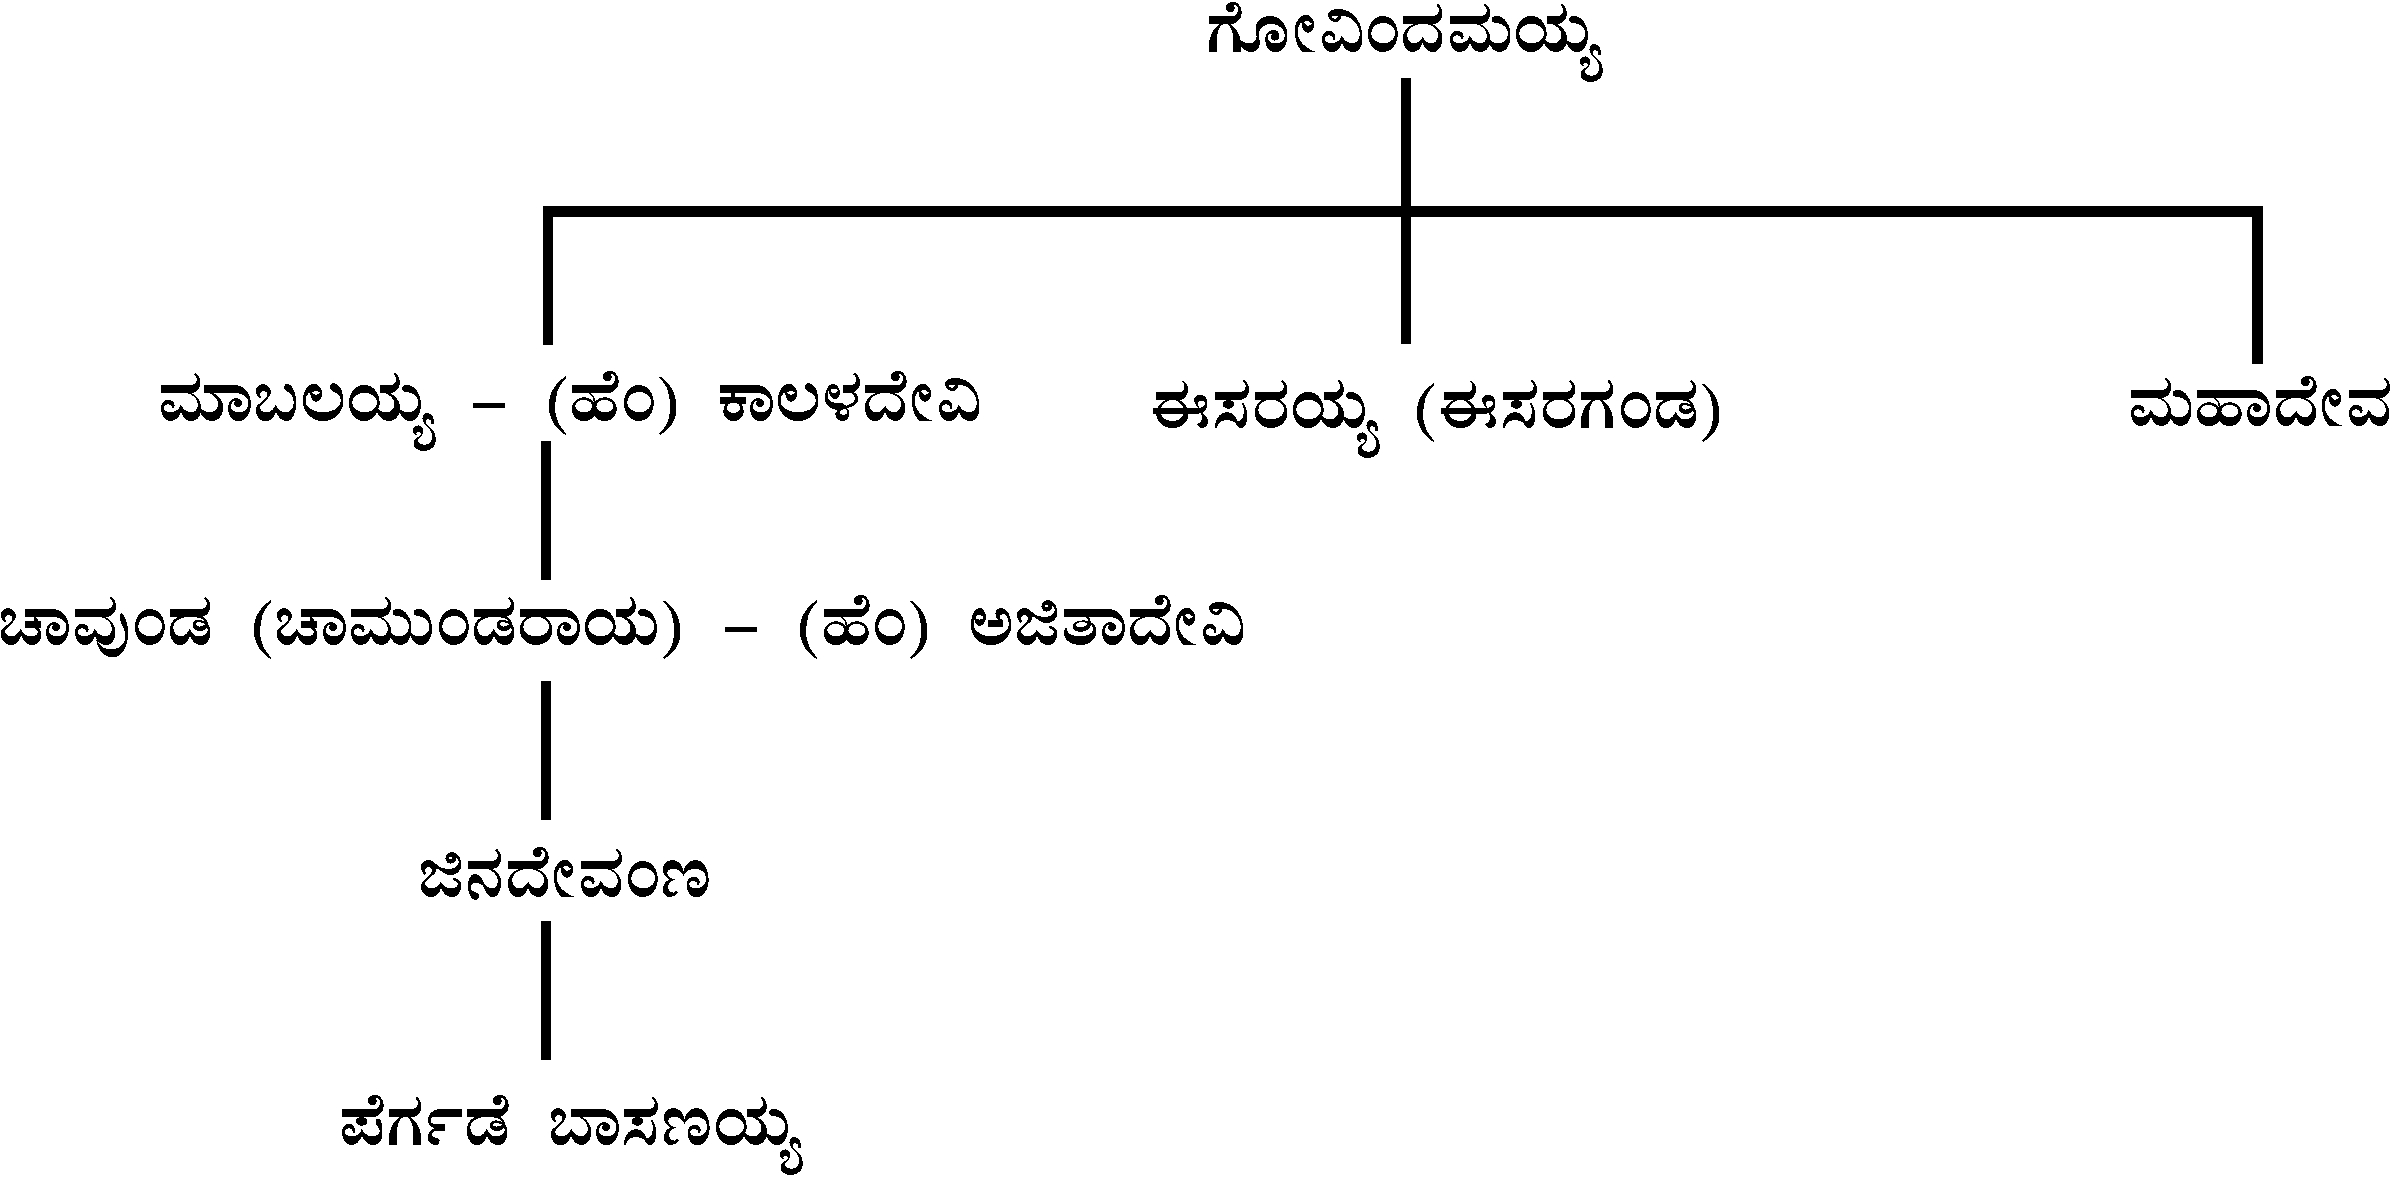
\includegraphics[scale=1.15]{images/chap3/chap3fig1.jpeg}
\end{figure}


\section*{ಹೆಗ್ಗಡೆ/ಪೆರ್ಗ್ಗಡೆ/ಪೆರಾಳ್ಕೆ ಹೆಗ್ಗಡೆ/ಮೇಲಾಳಿಕೆ}

ಪೆರ್ಗ್ಗಡೆ\index{ಪೆರ್ಗ್ಗಡೆ} ಎಂಬುದು ಮಂತ್ರಿ ಅಥವಾ ಅಮಾತ್ಯ ಪದವಿಗೆ ಸಮಾನವಾದ ಹುದ್ದೆಯಾಗಿತ್ತೆಂದು ತೋರುತ್ತದೆ. ಗಂಗರು ಮತ್ತು ಹೊಯ್ಸಳರ ಶಾಸನಗಳಲ್ಲಿ ಇದನ್ನು ಪೆರಾಳ್ಕೆ, ಮೇಲಾಳ್ಕೆ, ಮೇಲಾಳಿಕೆ\index{ಮೇಲಾಳಿಕೆ} ಎಂದು ಹೇಳಿದೆ. ಶ‍್ರೀಪುರುಷನು ಬಾಣವಂಶದ ಮಾಂಡಲಿಕ ದಿಂಡಿಗನ ಕೋರಿಕೆಯ ಮೇರೆಗೆ ಕೊವಳೆವೆಟ್ಟು\index{ಕೊವಳೆವೆಟ್ಟು} ಗ್ರಾಮವನ್ನು ಬ್ರಹ್ಮದೇಯವಾಗಿ ನೀಡಿದಾಗ, ಪೆರ್ಗ್ಗಡೆ ಕೊನ್ದಡಿಯು ಸಾಕ್ಷಿಯಾಗಿದ್ದನೆಂದು ಹೇಳಿದೆ.\endnote{ ಎಕ 7 ಮಂ 14 ಹುಳ್ಳೇನಹಳ್ಳಿ 8ನೇ ಶ.} ಗಂಗಪೆರ್ಮ್ಮಾನಡಿಯು ಕುನ್ದೂರು ನಾಡನ್ನು\index{ಕುನ್ದೂರು ನಾಡು} ಆಳುತ್ತಿದ್ದಾಗ, ಬಾಸಣಯ್ಯನೆಂಬುವವನು\index{ಬಾಸಣಯ್ಯ} ಅವನ ಪೆರ್ಗ್ಗಡೆಯೂ ಮಂತ್ರಿಯೂ ಆಗಿದ್ದನು.\textbf{ “ಸಮರಧಾರಧರಂ ರಾಜ್ಯಭರ ಧುರಂಧರಂಮಮಾತ್ಯ ಪದವೀ ವಿರಾಜಮಾನಂ.....ತಂತ್ರರಕ್ಷಾಮಣಿ ಮಂತ್ರಚಿನ್ತಾಮಣಿ ವಿನೇಯವಿಳಾಸಂ ಶ‍್ರೀಮತ್ಪೆರ್ಗ್ಗಡೆ ಬಾಸ(ಣಯ್ಯಂ)” }ಎಂದು ಬೇಲೂರು ಶಾಸನವು ಇವನನ್ನು ವರ್ಣಿಸಿದೆ.\endnote{ ಎಕ 7 ಮಂ 67 ಬೇಲೂರು 1022} ಈತನು ಬೇಲೂರಿನಲ್ಲಿ ಬೊಯ್ಸಿಕಟ್ಟೆಯನ್ನು ಕಟ್ಟಿಸಿ ತೂಬನ್ನಿಡಿಸಿ ಮಹಾದೇವರಿಗೆ ಗದ್ದೆಯನ್ನು, ಕೆರೆಗೆ ಬಿತ್ತುವಟ್ಟವನ್ನೂ ದತ್ತಿಯಾಗಿ ಬಿಟ್ಟನು. ಶ್ರವಣಬೆಳಗೊಳದ ಚಿಕ್ಕಬೆಟ್ಟದಲ್ಲಿ ಚಾಮುಂಡರಾಯನ ಬಸದಿಯ ಪಕ್ಕ ಬಂಡೆಯ ಮೇಲೆ “ಶ‍್ರೀಬಾಸ"\endnote{ ಎಕ 2 ಶ್ರಬೆ 106 ಚಿಕ್ಕಬೆಟ್ಟ 10ನೇ ಶ.} ಎಂಬ ಹಸ್ತಾಕ್ಷರವಿದೆ. ಅಲ್ಲಿರುವ ಲಕ್ಕಿದೊಣೆ(ಜಿನದೊಣೆ)ಯ ದಂಡೆಯ ಮೇಲೆ “ಶ‍್ರೀಬಾಸಣ್ಣನ ದಣ್ಡೆ\index{ಶ‍್ರೀಬಾಸಣ್ಣನ ದಣ್ಡೆ}"\endnote{ ಎಕ 2 ಶ್ರಬೆ 228 ಚಿಕ್ಕಬೆಟ್ಟ 10ನೇ ಶ.} ಎಂಬ ಬರಹವಿದೆ. ಇವೆಲ್ಲಾ ಹತ್ತನೇ ಶತಮಾನದ ಲಿಪಿಯಲ್ಲಿದ್ದು, ಬಾಸಣಯ್ಯನ ಹಸ್ತಾಕ್ಷರವಿರಬಹುದು. ಇವನು ಚಾಮುಂಡರಾಯನ ಮಗ ಅಥವಾ ಮೊಮ್ಮಗನಾಗಿರಬಹುದು. ಚಾಮುಂಡರಾಯನ ನಂತರ ಗಂಗರ ಬಳಿ ಮಂತ್ರಿಪದವಿ\-ಯಲ್ಲಿದ್ದಿರಬಹುದು. ಪೆರಾಳ್ಕೆ ಹೆಗ್ಗಡೆ ಎಂಬುದು ಒಂದು ಪದವಿ. ಈ ಪೆರಾಳ್ಕೆಯೇ ಮುಂದೆ ಮೇಲಾಳಿಕೆ ಎಂದಾಗಿರಬಹುದು. ಶ‍್ರೀಮತು ಪೆರಾಳ್ಕೆ ಹೆಗ್ಗಡೆ ಚನ್ದಯ್ಯನು\index{ಪೆರಾಳ್ಕೆ ಹೆಗ್ಗಡೆ ಚನ್ದಯ್ಯ} ತೊಳಂಚೆಯ ಗೋಳಗವುಡನು ಅಂಕಕಾರ ದೇವರಿಗೆ ದತ್ತಿ ಬಿಟ್ಟರೆಂದು ತಿಳಿದುಬರುತ್ತದೆ.\endnote{ ಎಕ 6 ಕೃಪೇ 51 ತೊಣಚಿ 10ನೇ ಶ.} “ಸಾಮಂತ ದೇಕೆಯನಾಯಕರ ಮೇಲಾಳಿಕೆ” ಎಂದು ಹೊಯ್ಸಳರ ಕಾಲದ ಹೊನ್ನೇನಹಳ್ಳಿ ಶಾಸನದಲ್ಲಿ ಹೇಳಿದೆ.\endnote{ ಎಕ 7 ನಾಮಂ 106 ಹೊನ್ನೇನಹಳ್ಳಿ 1180}

\section*{ಕರಣ (ಶ‍್ರೀಕರಣ/ಪ್ರಮುಖ ಕರಣ)}

ಕರಣರೂ ರಾಜರ ಅಧಿಕಾರಿಗಳು. ಇವರಲ್ಲಿ ಪ್ರಮುಖರನ್ನು ಶ‍್ರೀಕರಣ\index{ಶ‍್ರೀಕರಣ} ಅಥವಾ ಪ್ರಮುಖ ಕರಣ\index{ಪ್ರಮುಖ ಕರಣ} ಎಂದು ಕರೆಯುತ್ತಿದ್ದರೆಂದು ಹೇಳಬಹುದು. ಇಮ್ಮಡಿ ಬೂತುಗನು "ಪ್ರಮುಖ ಕರಣನಾದ ಶ‍್ರೀಮತ್​ ಪುಣಿಗದ ಮಾಚಯ್ಯನಿಗೆ\index{ಪುಣಿಗದ ಮಾಚಯ್ಯ}" ಆದೇಶ ನೀಡಿ, ಬಡಗೆರೆನಾಡೊಳಗಣ ಧನುಗೂರನ್ನು\index{ಧನಗೂರು (ಧನುಗೂರು - ಧನುರು)} ಆಚಮಂಗೆ ಕಲ್ನಾಡಾಗಿ\index{ಕಲ್ನಾಡು} ಕೊಡುತ್ತಾನೆ. ಇದಕ್ಕೆ ಕಸವಯ್ಯ, ನಾಗವರ್ಮ್ಮಯ್ಯ, ರೇವಣಯ್ಯ ಇವರ ಅಕ್ಕರ(ಸಾಕ್ಷಿ) ಇದೆ. ಇವರು ಕರಣರಾಗಿದ್ದು, ಪುಣಿಗದ ಮಾಚಯ್ಯನು ಇವರಿಗೆಲ್ಲಾ ಪ್ರಮುಖ ಕರಣನಾಗಿದ್ದನೆಂದು ಹೇಳಬಹುದು.\endnote{ ಎಕ 7 ಮವ 50 ಧನಗೂರು 960}

\section*{ಗಾಮುಂಡರು}
\index{ಗಾಮುಂಡರು}

ಗ್ರಾಮದ ಆಡಳಿತವನ್ನು ನೋಡಿಕೊಳ್ಳುವವರು ಗಾಮುಂಡರು. ಗ್ರಾಮದ ಒಡೆಯರಾದ ಇವರ ಕರ್ತವ್ಯ ಹೊಣೆಗಾರಿಕೆ ಹೆಚ್ಚಿನದಾಗಿತ್ತು.\endnote{ ನಾಗಯ್ಯ, ಡಾ.ಜೆ.ಎಮ್., ಆರನೆಯ ವಿಕ್ರಮಾದಿತ್ಯನ ಶಾಸನಗಳು, ಪುಟ 253} ಗಂಗರ ಕಾಲದ ಸ್ಥಳೀಯ ಆಡಳಿತದಲ್ಲಿ ಗಾಮುಂಡರ ಪಾತ್ರ ಪ್ರಮುಖವಾಗಿತ್ತೆಂದು ತೋರುತ್ತದೆ. ಇವರನ್ನೇ “ಷಣ್ಣವತಿ ಸಹಸ್ರ ವಿಷಯ ಪ್ರಕೃತಃ\index{ಷಣ್ಣವತಿ ಸಹಸ್ರ ವಿಷಯ ಪ್ರಕೃತಃ (ತಯಃ)}” ಎಂದೂ “ನಾಡಿಗರು\index{ನಾಡಿಗರು}” ಎಂದೂ ಕರೆದಿರಬಹುದು. ಕನ್ನಡದಲ್ಲಿ ಇವರನ್ನು ` ಬಲ್ಲವರು\index{ಬಲ್ಲವರು}' ಎಂದು ಹೇಳಿದೆ. ಅನೇಕ ಶಾಸನಗಳಲ್ಲಿ ಈ ಗಾಮುಂಡರು ಸಾಕ್ಷಿಗಳಾಗಿದ್ದಾರೆ. ಇವರಲ್ಲೇ ಪ್ರಮುಖರನ್ನು ಗಾಮುಂಡಸ್ವಾಮಿ ಎಂದು ಕರೆಯತ್ತಿದ್ದರೆಂದು ತಿಳಿದುಬರುತ್ತದೆ. ಗಾಮುಂಡರನ್ನು “ಒಕ್ಕಲು” ಎಂದೂ ಕರೆದಿದೆ. ನಾಡು ಮತ್ತು ಒಕ್ಕಲು ಎಂಬುದು ಗ್ರಾಮ ಸಭೆಯಾಗಿರಬಹುದು.\endnote{ \engfoot{Dixith, Dr.G.S., Local Self Government in Mediaeval Karnataka, pp.57-60}}

ನೊಳಂಬಾಧಿರಾಜನು ರಾಜ್ಯವಾಳುತ್ತಿದ್ದಾಗ ತೈರೂರ ಕೌಣ್ಡಿಲ್ಯ ಗೋತ್ರದ ಗಾಮುಣ್ಡಸ್ವಾಮಿಗಳ\index{ಗಾಮುಂಡಸ್ವಾಮಿ} ಮಗ ನಾಗಮಯ್ಯನು\index{ನಾಗಮಯ್ಯ} ಕಲ್ಲದೇಗುಲವನ್ನು\index{ಕಲ್ಲದೇಗುಲ} ಮಾಡಿಸಿ ಭೂಮಿಯನ್ನು ಬಿಡುತ್ತಾನೆ.\endnote{ ಎಕ 7 ಮ 57 ತಾಯಲೂರು 895-96} ಗಾಮುಣ್ಡಸ್ವಾಮಿಯು ಗಾಮುಂಡರಿಗೆಲ್ಲ ಒಡೆಯ ಅಥವಾ ಮುಖ್ಯಸ್ಥನೆಂದು ಹೇಳಬಹುದು. ನಾಗಮಯ್ಯನಿಗೆ ಗೋತ್ರವನ್ನು ಹೇಳಿರುವುದರಿಂದ ವೈದಿಕರೂ ಕೂಡಾ ಗಾಮುಂಡರಾಗಿರು\-ತ್ತಿದ್ದರೆಂದು ಹೇಳಬಹುದು. ಮಾರಸಿಂಹನ\index{ಮಾರಸಿಂಹ (ಎರೆಯಪ್ಪ)} ಕಾಲದಲ್ಲಿ ತಿಪ್ಪೆರೂರನ್ನು\index{ತಿಪ್ಪೆರೂರು} ಬ್ರಹ್ಮದೇಯವನ್ನಾಗಿ ನೀಡಿದಾಗ ಅದಕ್ಕೆ ಮುದುಗುಪ್ಪೆಯ\index{ಮುದುಗುಪ್ಪೆ } ಮಾರಸಿಂಗ ಗಾಮುಣ್ಡರು, ಎರೆಗಂಗ ಗಾಮುಣ್ಡರು, ಮರವೂರ ಉರ್ಕಣೆ ಗಾಮುಣ್ಡರು, ಭೀಮಗಾಮುಣ್ಡರು, ಬೆಳ್ಳಿಮಾಣಿಯ ಶ‍್ರೀಯಗಾಮುಣ್ಡರು, ಕುಪ್ಪಾಲ್ಮಾದವರುಂ, ಪೆರ್ಬ್ಬೞ ಉತ್ತುಮ ಗಾಮುಣ್ಡರು, ಕುನ್ದಗಾಮುಣ್ಡರು, ಸಂಗಮದ\break ಪೃಥುವೀ ಗಾಮುಣ್ಡರು, ರಿಪುರಾಮ ಗಾಮುಣ್ಡರು ಇಷ್ಟೂ ಜನರು ನರಸಾಕ್ಷಿಯಾಗಿರುತ್ತಾರೆ.\endnote{ ಎಕ 6 ಶ‍್ರೀಪ 66 ಗಂಜಾಮ್ 8ನೇ ಶ.} ಇದರಿಂದ ಸುತ್ತಮುತ್ತಲ ಅನೇಕ ಊರುಗಳ ಗಾಮುಂಡರು\index{ಗಾಮುಂಡರು} ಭಾಗವಹಿಸಿದ್ದರೆಂದು ತಿಳಿಯಬಹುದು. ಬಿಜ್ಜೈಯನು ಸಾವಿಯಬ್ಬೇಶ್ವರಕ್ಕೆ\index{ಸಾವಿಯಬ್ಬೇಶ್ವರ} ಭೂಮಿಯನ್ನು ಬಿಟ್ಟಾಗ ಚಾವುಣ್ಡ ಗಾಮುಣ್ಡ, ಶ‍್ರೀ ಕಣ್ನಂಬಾಡಿಯ\index{ಕಣ್ನಂಬಾಡಿ} ಪೊನ್ನಗಾವುಣ್ಡ, ಹಾರಪ್ಪಂಗಳ ಮಗ ಬಾಚಿಗ, ಅಪತಿಯ ತೌಳಿಯಮ್ಮ ಸಾಕ್ಷಿಗಳಾಗಿರುತ್ತಾರೆ.\endnote{ ಎಕ 6 ಪಾಂಪು 43 ಕನ್ನಂಬಾಡಿ 10ನೇ ಶ.} ಶ‍್ರೀಪುರುಷನ ಕಾಲದಲ್ಲಿ ಕೊವಳೆವೆಟ್ಟು ಗ್ರಾಮವನ್ನು ಬ್ರಹ್ಮದೇಯವಾಗಿ ನೀಡಿದಾಗ ಅದಕ್ಕೆ ದಿಣ್ಡಿಗ ನಾಡಿಯರು\index{ದಿಣ್ಡಿಗ ನಾಡಿಯರು} (ದಿಂಡಿಗ ನಾಡಿನ ನಾಡಗವುಡರು) ಸಾಕ್ಷಿಗಳಾಗಿರುತ್ತಾರೆ.

\textbf{ಷಣ್ಣವತಿ ಸಹಸ್ರ ವಿಷಯ ಪ್ರಕೃತಯ\index{ಷಣ್ಣವತಿ ಸಹಸ್ರ ವಿಷಯ ಪ್ರಕೃತಃ (ತಯಃ)}:} ಗಂಗರ ಕೆಲವು ತಾಮ್ರಪಟಗಳಲ್ಲಿ ದಾನ ನೀಡಿದಾಗ “ಅಸ್ಯ ದಾನಸ್ಯ ಸಾಕ್ಷಿಣಃ ಚಾತುರ್ವ್ವೈದ್ಯ ಸಹಿತಃ ಷಣ್ಣವತಿಸಹಸ್ರವಿಷಯ ಪ್ರಕೃತಯಃ ಆಸ್ಥಾಯಿಕಾ ಪುರಷಾಶ್ಚ”.\endnote{ ಎಕ 7 ಮಂ 35 ಹಳ್ಳೆಗೆರೆ 713} ಎಂಬ ಒಕ್ಕಣೆಯು ಕಾಣಿಸಿಕೊಳ್ಳುತ್ತದೆ. ಷಣ್ಣವತಿ ಸಹಸ್ರ ವಿಷಯ ಎಂದರೆ ಗಂಗವಾಡಿ 96000 ಎಂದು ಅರ್ಥೈಸಬಹುದು. ಈ ನಾಡಿನ ಮುಖ್ಯಸ್ಥರು ಹಾಗೂ ಆಸ್ಥಾನದಲ್ಲಿದ್ದ ಪುರುಷರು ಅಂದರೆ ಅಧಿಕಾರಿಗಳು ಅಥವಾ ಮಂತ್ರಿ ಪರಿಷತ್ತಿನವರು ಇದಕ್ಕೆ ಸಾಕ್ಷಿಯಾಗಿರುತ್ತಾರೆ ಎಂಬುದು ಇದರ ಅರ್ಥವೆಂದು ಹೇಳಬಹುದು. ಇದೇ ಒಕ್ಕಣೆಯು ನಾಗಮಂಗಲ ತಾಲ್ಲೂಕಿನ ದೇವರಹಳ್ಳಿ,\endnote{ ಎಕ 7 ನಾಮಂ 149 ದೇವರಹಳ್ಳಿ 776} ಚಾಮರಾಜನಗರ ತಾಲ್ಲೂಕಿನ ಕೆರೆಹಳ್ಳಿ,\endnote{ ಎಕ 4 ಚಾನ 354 ಕೆರೆಹಳ್ಳಿ 904} ಕುಲಗಾಣಾ,\endnote{ ಎಕ 4 ಚಾನ 347 ಕುಲಗಾಣ 8ನೇ ಶ.} ಮೈಸೂರು ಜಿಲ್ಲೆ ಸಾಲಿಗ್ರಾಮ,\endnote{ ಎಕ 5 ಕೃನಾ 48 ಸಾಲಿಗ್ರಾಮ 725, ಕೃನಾ 49 ಸಾಲಿಗ್ರಾಮ 819} ತಾಮ್ರಶಾಸನಗಳಲ್ಲೂ ಇದೆ. ಮಳವಳ್ಳಿ ತಾಲ್ಲೂಕಿನ ಯಮ್ಮದೂರು ಶಿಲಾ ಶಾಸನದಲ್ಲಿ ಇದರ ಕನ್ನಡ ಅನುವಾದವಿದ್ದಂತಿದೆ. “ತ್ತೊಮ್ಭತ್ತಱು ಸಸಿರರ್ಬ್ಬಲ್ಲವರೆಮ್ಮೞ್ದಕ್ಕೆ ನೆಲ್ಲಕೂೞಣಲಾಗೊದೆನ್ದು ಬಿಟ್ಟದತ್ತಿ” ಎಂದು ಹೇಳಿದೆ. ತೊಂಬತ್ತರುಸಾಸಿರದ ಬಲ್ಲವರು\index{ತೊಂಬತ್ತರುಸಾಸಿರದ ಬಲ್ಲವರು} ಎಮ್ಮಳ್ದಕ್ಕೆ\index{ಎಮ್ಮಳ್ದಕ್ಕ} ಗ್ರಾಮವನ್ನು ನೆಲ್ಲಕೂಳಣವಾಗಿ\index{ನೆಲ್ಲ ಕೂಳಣ} ದತ್ತಿ ಬಿಟ್ಟಿದ್ದಾರೆ. ಬಲ್ಲವರು ಅಂದರೆ ಸ್ಥಳೀಯ ಆಡಳಿತದ ಮುಖ್ಯಸ್ಥರು ದಾನಕ್ಕೆ ಸಾಕ್ಷಿಗಳಾಗಿ ನಿಂತಿದ್ದಾರೆ. ಎಪಿಗ್ರಾಫಿಯಾ ಸಂಪಾದಕರು, 96000 ನಾಡಿನ ಗ್ರಾಮ ನಿವಾಸಿಗಳು ಅಂದರೆ ಬಲ್ಲವರು ಎಂದು ಸರಿಯಾಗಿ ಅರ್ಥೈಸಿ ನಂತರ ಇದು ಬಿಲ್ಲವರಿರಬೇಕು, ಬಿಲ್ಲವರ ಸಂಘಕ್ಕೆ ದತ್ತಿಬಿಡಲಾಗಿದೆ ಎಂದು ಹೇಳಿದ್ದಾರೆ.\endnote{ ಎಪಿಗ್ರಾಫಿಯಾ ಕರ್ನಾಟಿಕಾ, ಸಂಪುಟ 7, ಪೀಠಿಕೆ, ಪುಟ xlviii}

\textbf{ಬೀೞವೃತ್ತಿ\index{ಬೀೞವೃತ್ತಿ (ಬೀಳವೃತ್ತಿ)}:} ಬೀೞವೃತ್ತಿಯು ಅಧಿರಾಜರು ಮತ್ತು ಸಾಮಂತರ ಸಂಬಂಧವನ್ನು ಸೂಚಿಸುತ್ತದೆ ಎಂದು ಡಾ.ಎಂ.\-ಚಿದಾನಂದಮೂರ್ತಿಯವರು ಹೇಳಿದ್ದರೆ,\endnote{ ಚಿದಾನಂದಮೂರ್ತಿ, ಡಾ॥ ಎಂ., ಕನ್ನಡ ಶಾಸನಗಳ ಸಾಂಸ್ಕೃತಿಕ ಅಧ್ಯಯನ, ಪುಟ 340-41} ರಾಜನಿಗೆ ನಿಷ್ಠಾವಂತರಾಗಿದ್ದವರು, ಗರುಡರಾಗಿದ್ದವರು ಬೀೞಾನುವೃತ್ತಿಯಿಂದ ಆಳುತ್ತಿದ್ದರು. ಇವರನ್ನು ಸಾಮಂತರನ್ನಾಗಿ ನೇಮಿಸಲಾಗುತ್ತಿತ್ತು ಎಂದು ನಾಗಯ್ಯನವರು ಹೇಳಿದ್ದಾರೆ\endnote{ ನಾಗಯ್ಯ, ಡಾ॥ ಜೆ.ಎಂ., ಆರನೆಯ ವಿಕ್ರಮಾದಿತ್ಯನ ಶಾಸನಗಳು-ಒಂದು ಅಧ್ಯಯನ, ಪುಟ 81}. ನೀತಿಮಾರ್ಗ ಪೆರ್ಮ್ಮಾನಡಿಯ ಕಾಲದಲ್ಲಿ, ಆರಂಭಲ್ಲ(ವ)ನು\index{ಆರಂಭಲ್ಲ} ಇದುಳೆಯನ್ನು\index{ಇದುಳೆ} ಬೀಳವೃತ್ತಿಯಿಂದ ಆಳುತ್ತಿದ್ದನು.\endnote{ ಎಕ 7 ನಾಮಂ 127 ಕಾರಬಯಲು 9ನೇ ಶ.} ಇವನು ಗಂಗರ ಪರವಾಗಿ ರಾಷ್ಟ್ರಕೂಟರ ಸೇನೆಯ ಮೇಲೆ ಹೋರಾಡಿ ಮಡಿದನು.

\newpage

\textbf{ಪೆರ್ಮಾನಡಿ ಜೀವಿತ\index{ಪೆರ್ಮಾನಡಿ ಜೀವಿತ}:} ಪೆರ್ಮಾನಡಿ ಜೀವಿತವೂ ಬೀೞವೃತ್ತಿಯಂತಹದೇ ಆಗಿದೆ. ಗಂಗಪೆರ್ಮ್ಮಾನಡಿಯು\index{ಗಂಗಪೆರ್ಮ್ಮಾನಡಿ} ಕುನ್ದೂರು ನಾಡನ್ನು\index{ಕುನ್ದೂರು ನಾಡು} ಆಳುತ್ತಿದ್ದಾಗ, ನಾಲಯ್ಯನಿಗೆ\index{ನಾಲಯ್ಯ} ಪೆರ್ಮ್ಮಾನಡಿ ಜೀವಿತವಾಗಿ, ಬೇಲೂರನ್ನು ದತ್ತಿ ಬಿಡಲಾಗಿದೆ.\endnote{ ಎಕ 7 ಮಂ 67 ಬೇಲೂರು 1022} “ಸುಮಾರು 890ರಲ್ಲಿ ಗಂಗರಾಜ ಶ‍್ರೀಮತ್​ ಪೆರ್ಮಾನಡಿಗಳು ಜೆಡಲ ಎಱೆಯಂಗ ಗಾವುಂಡನ ಮಗನಿಗೆ ಪೆರ್ಮಾಡಿ ಪಟ್ಟಂಗಟ್ಟಿದನೆಂದು ತಿಳಿದುಬರುತ್ತದೆ.\endnote{ ಚಿದಾನಂದಮೂರ್ತಿ, ಡಾ॥ ಎಂ., ಪೂರ್ವೋಕ್ತ, ಪುಟ 360}

\section*{ಹೊಯ್ಸಳರ ಕಾಲದ ಆಡಳಿತ ವ್ಯವಸ್ಥೆ}

ಹೊಯ್ಸಳರ ಆಡಳಿತ ವ್ಯವಸ್ಥೆಯೂ ಅವರಿಗಿಂತ ಹಿಂದೆ ಈ ಭಾಗದಲ್ಲಿ ಆಡಳಿತ ನಡೆಸಿದ ಗಂಗರು ಮತ್ತು ಅವರ ಸಾಮ್ರಾಟರಾದ ಕಲ್ಯಾಣದ ಚಾಲುಕ್ಯರ ಆಡಳಿತ ವ್ಯವಸ್ಥೆಯನ್ನು ಅಳವಡಿಸಿಕೊಂಡರೂ ಅವುಗಳ ಒಂದು ಸುಧಾರಿತ ರೂಪದಲ್ಲಿತ್ತೆಂದು ಹೇಳಬಹುದು. ಹೊಯ್ಸಳರ ಕಾಲದಲ್ಲಿ ಗಂಗರು ಮತ್ತು ಕಲ್ಯಾಣದ ಚಾಲುಕ್ಯರ ಆಡಳಿತದಲ್ಲಿದ್ದ ಅಧಿಕಾರಿಗಳ ವ್ಯವಸ್ಥೆಯೇ ಇದ್ದರೂ ಕೆಲವೊಂದು ಹೊಸ ಅಧಿಕಾರಿ ಹುದ್ದೆಗಳಿದ್ದುದು ಕಂಡುಬರುತ್ತದೆ. ಕೇಂದ್ರೀಯ ಆಡಳಿತ ವ್ಯವಸ್ಥೆಯಲ್ಲಿ ರಾಜನೇ ದೇವರು. “ಒಂದು ದೇಶದ ಜನಜೀವನವು ಆ ದೇಶದ ರಾಜನನ್ನು ಅವಲಂಬಿಸಿದ್ದಿತು. ಅವನ ಏಳುಬೀಳುಗಳೇ ರಾಜ್ಯದ ಏಳುಬೀಳುಗಳು”,\endnote{ ಚಿದಾನಂದಮೂರ್ತಿ, ಡಾ॥ ಎಮ್., ಕನ್ನಡ ಶಾಸನಗಳ ಸಾಂಸ್ಕೃತಿಕ ಅಧ್ಯಯನ, ಪುಟ 322-323} ಎಂಬ ಹೇಳಿಕೆಗಳು ಹೊಯ್ಸಳರ ಕಾಲಕ್ಕೂ ಕೂಡಾ ಅನ್ವಯಿಸುತ್ತದೆಂದು ಹೇಳಬಹುದು.

ಜಿಲ್ಲೆಯ ಹೊಯ್ಸಳ ಶಾಸನಗಳಲ್ಲಿ, ಹೊಯ್ಸಳ ರಾಜರನ್ನು ದೇವರೆಂದೇ ಸಂಬೋಧಿಸಲಾಗಿದೆ. ತ್ರಿಭುವನಮಲ್ಲ ಪೊಯ್ಸಳದೇವ, ತ್ರಿಭುವನಮಲ್ಲ ವಿನಯಾದಿತ್ಯ ಪೊಯ್ಸಳದೇವರಸರು\index{ಪೊಯ್ಸಳದೇವರಸರು}, ವಿಷ್ಣುವರ್ಧನ ದೇವರು\index{ವಿಷ್ಣುವರ್ಧನ (ದೇವರು) (ಹೊಯ್ಸಳರ ದೊರೆ)}, ಬಲ್ಲಾಳ ದೇವರಸರು\index{ಬಲ್ಲಾಳ ದೇವರಸರು}, ನಾರಸಿಂಹದೇವರಸರು\index{ನಾರಸಿಂಹದೇವ}, ಸೋಮೇಶ್ವರ ದೇವರಸರು\index{ಸೋಮೇಶ್ವರ ದೇವರಸರು} ಎಂಬುದಾಗಿ ಹೇಳಿರುವುದು ರಾಜನೇ ಪ್ರತ್ಯಕ್ಷ ದೈವ ಎಂಬುದನ್ನು ಸೂಚಿಸುತ್ತವೆ. ವಿನಯಾದಿತ್ಯನನ್ನು ಆದಿವರಾಹನಿಗೂ, ವಿಷ್ಣುವರ್ಧನನ್ನು ವಿಷ್ಣುವಿಗೂ, ನರಸಿಂಹನನ್ನು ಕಂಬದಿಂದ ಉದಿಸಿದ ನರಸಿಂಹನಿಗೂ ಹೋಲಿಸಿರುವುದು ಈ ಹಿನ್ನೆಲೆಯಲ್ಲಿಯೇ. “ವಿಕ್ರಮಾದಿತ್ಯನ ಸಾಮ್ರಾಜ್ಯದಲ್ಲಿ ಮಹಾಮಂಡಳೇಶ್ವರರು, ಮಹಾಸಾಮಂತರು, ಪ್ರಭುಗಾವುಂಡರು ಮತ್ತು ಗಾವುಂಡರು ಎಂಬ ನಾಲ್ಕು ತೆರನಾದ ಪ್ರಭುವರ್ಗದವರು ಒಡೆಯರಾಗಿ ಆಳುತಿದ್ದರು".\endnote{ ನಾಗಯ್ಯ ಡಾ॥ ಜೆ.ಎಂ., ಆರನೆಯ ವಿಕ್ರಮಾದಿತ್ಯನ ಶಾಸನಗಳು, ಒಂದು ಅಧ್ಯಯನ, ಪುಟ 151-52} “ಶಾಸನಗಳಲ್ಲಿ ಅಧಿಕಾರಿಗಳಿಗೆ ಸಂಬಂಧಪಟ್ಟಂತೆ ಅನೇಕ ಪಾರಿಭಾಷಿಕ ಶಬ್ದಗಳು ಬರುತ್ತವೆ. ಈವರೆಗೆ ಈ ಎಲ್ಲ ಪದಗಳು ಹುದ್ದೆಗಳನ್ನು ಸೂಚಿಸುತ್ತವೆಯೆಂದು ನಂಬಲಾಗಿದೆ. ಆದರೆ ಇವುಗಳನ್ನು ಪದವಿ, ಶ್ರೇಣಿ, ಮತ್ತು ಹುದ್ದೆ ಎಂಬ ಮೂರು ವರ್ಗವನ್ನಾಗಿ ವಿಂಗಡಿಸಬಹುದೆಂದು ತೋರುತ್ತದೆ. ಮಹಾಮಾತ್ಯ, ಮಹಾಪ್ರಧಾನ, ಸಚಿವ\enginline{-}ಮಂತ್ರಿ, ಪಸಾಯಿತ ಎಂಬಿವು ಪದವೀ ಸೂಚಿಗಳಾದರೆ, ಮಹಾಸಾಮಂತಾಧಿಪತಿ, ಮಹಾಪ್ರಚಂಡ ದಂಡನಾಯಕ ಮತ್ತು ದಂಡನಾಯಕ, ಎಂಬಿವು ಅಧಿಕಾರ ಶ್ರೇಣಿಗಳಾಗಿದ್ದು, ರಾಜಾಧ್ಯಕ್ಷ, ಅಂತಃಪುರಾಧ್ಯಕ್ಷ, ನಿಯೋಗಿ, ಪಡೆವಳ, ಪೆರ್ಗಡೆ, ಪಡಿಹಾರ, ಹಡಪವಳ, ಕರಣಿಕ\enginline{-}ಸೇನಬೋವ\enginline{-}ಕುಲಕರಣಿ, ತಳಾರ, ಎಂಬಿವು ನೇರವಾಗಿ ಹುದ್ದೆಯನ್ನು ಸೂಚಿಸುತ್ತವೆ ಎಂದು ಹೇಳಲಾಗಿದೆ".\endnote{ ಅದೇ, ಪುಟ 277-78}

\textbf{ಮಹಾಮಂಡಳೇಶ್ವರರು\index{ಮಹಾಮಂಡಲೇಶ್ವರರು}/ಮಂಡಳೇಶ್ವರರು\index{ಮಂಡಳೇಶ್ವರ} ಅಥವಾ ಮಂಡಳಿಕರು\index{ಮಂಡಳಿಕರು}/ ನಾಡಮಂಡಳೀಕರು\index{ನಾಡಮಂಡಳೀಕರು}:} ಹೊಯ್ಸಳರು ಕಲ್ಯಾಣದ ಚಾಲುಕ್ಯರ ಮಹಾಮಂಡಳೇಶ್ವರರಾಗಿದ್ದರು.\endnote{ ನಾಗಯ್ಯ, ಡಾ॥ ಜೆ.ಎಮ್. ಆರನೆಯ ವಿಕ್ರಮಾದಿತ್ಯನ ಶಾಸನಗಳು, ಪುಟ 174-180} ಇವರು ಮಹಾಮಂಡಳೇಶ್ವರರ ಮಹಾಮಂಡಳೇಶ್ವರರಾಗಿದ್ದರು ಎಂದು ಹೇಳಬಹುದು.\endnote{ ಅದೇ, ಪುಟ 153} ಮಹಾಮಂಡಳೇಶ್ವರರಾಗಿದ್ದರಿಂದ ಅವರ ಕೈಕೆಳಗೆ ಮತ್ತೆ ಮಹಾಮಂಡಳೇಶ್ವರರು, ಮಂಡಳೇಶ್ವರರು, ಮಂಡಲಿಕರು ಹೆಚ್ಚಾಗಿ ಇರಲಿಲ್ಲವೆಂದು ಹೇಳಬಹುದು. ಇಮ್ಮಡಿ ಬಲ್ಲಾಳನ ಕಾಲದಿಂದ ಹೊಯ್ಸಳರು ತಮ್ಮನ್ನು ಚಕ್ರವರ್ತಿ\-ಗಳೆಂದು ಹೇಳಿಕೊಂಡಿದ್ದು, ಅವರ ಕೈಕೆಳಗೆ ರಾಜ್ಯದ ಕೆಲವು ಭಾಗಗಳನ್ನು ಸ್ವತಂತ್ರವಾಗಿ ಆಳ್ವಿಕೆ ನಡೆಸಿಕೊಂಡು, ಸೇನಾಪಡೆಗೆ ಬೇಕಾದ ಸೈನಿಕರನ್ನು ಒದಗಿಸುತ್ತಿದ್ದವರೇ ಮಹಮಂಡಲೇಶ್ವರರು, ಸಾಮಂತರು ಎಂದು ಹೇಳಬಹುದು.\endnote{ \engfoot{Radha Patel, Dr. M., Life and Times of Hoysala Narasimha III, pp. 41}} ಮಂಡ್ಯ ಜಿಲ್ಲೆಯ ಶಾಸನಗಳಲ್ಲಂತೂ ಇವರ ಉಲ್ಲೇಖ ಕಡಿಮೆ. ಎರೆಯಂಗನ ಕಾಲದಲ್ಲಿ ತೆಳರಕುಲತಿಲಕ\index{ತೆಲ್ಲ (ತೆಳಂ) ಕುಲತಿಲಕ} ನಗರುರ ಸೋಮಯ್ಯನು\index{ನಗರುರ ಸೋಮಯ್ಯ}, ಬಂಕಿನಾಡನ್ನು\index{ಬಂಕಿನಾಡು} ನಾಡ ಮಂಡಳಿಕನಾಗಿ ಆಳುತ್ತಿದ್ದನು.\endnote{ ಎಕ 7 ಮ 104 ಹಾಗಲಹಳ್ಳಿ 11ನೇ ಶ.} ಸೋಮೇಶ್ವರನ ದಂಡನಾಯಕರುಗಳಾಗಿದ್ದ ಬೋಗೈಯ\index{ಬೋಗೈಯ} ಮತ್ತು ಮುರಾರಿ ಮಲ್ಲಯ್ಯ\index{ಮುರಾರಿ ಮಲ್ಲಯ್ಯ} ದಂಡನಾಯಕರು ಮಂತ್ರಿಗಳಾಗಿದ್ದರು. ಇವರಲ್ಲಿ ಬೋಗೈಯ್ಯ ದಂಡನಾಯಕನು \textbf{ಮಂಡಲಿಕ ಮನ್ನೆಯಸೂನು\index{ಮಂಡಲಿಕ ಮನ್ನೆಯಸೂನು}} ಆಗಿದ್ದನು.\endnote{ ಎಕ 6 ಕೃಪೇ 39 ಗೋವಿಂದನಹಳ್ಳಿ 1236} ಇವನು ಕಬ್ಬಹು ನಾಡನ್ನು ಆಳುತ್ತಿದ್ದಿರಬಹುದು. ಇವರು \textbf{“ನಾನಾ ಸಾಮಂತ ಕಾಂತಾ ಕಚ ಹಠಹರಣ”} ರಾಗಿದ್ದರೆಂದು ಶಾಸನ ಹೇಳುತ್ತದೆ. ಅಂದರೆ ಇವರು ಮಂಡಲಿಕರು ಮತ್ತು ಸಾಮಂತರಿಗೆ ಒಡೆಯರಾಗಿದ್ದರೆಂದು ಊಹಿಸಬಹುದು.

\newpage

ಮುಮ್ಮಡಿ ಬಲ್ಲಾಳನ ಕಾಲದಲ್ಲಿ ಶ‍್ರೀಮನ್​ ಮಹಾಮಂಡಲೇಶ್ವರ ಕಮಳರಾಜ ತಂಮಯ ನಾಗರಸರ ನೇತೃತ್ವದಲ್ಲಿ, ಹದಿನೆಂಟು ಸಮಯದವರು ಸೇರಿ ಕೆಲವು ಕಟ್ಟುಪಾಡುಗಳನ್ನು ಜಾರಿಗೆ ತಂದಂತೆ ಮದ್ದೂರಿನ ತ್ರುಟಿತ ಶಾಸನದಿಂದ ತಿಳಿದುಬರುತ್ತದೆ.\endnote{ ಎಕ 7 ಮ 15 ಮದ್ದೂರು} ಶಾಸನದಲ್ಲಿ ನಾಡರಸರಾದ\index{ನಾಡರಸ} ಬಿಮಿಸೆಟ್ಟಿ\index{ಬಿಮಿಸೆಟ್ಟಿ}, ಯೋಗಗೌಡ\index{ಯೋಗಗೌಡ} ಇವರ ಉಲ್ಲೇಖವಿದ್ದು ಇವರನ್ನು ಸಮಸ್ತ ನಾಡಾಳ್ವರು ಎಂದು ಹೇಳಿದೆ. ಇವರು ಮಹಾಂಡಳೇಶ್ವರರ ಕೈಕೆಳಗಿನ ವಂಶಪಾರಂಪರ್ಯ ಅಧಿಕಾರಿಗಳಾಗಿದ್ದರೆಂದು ಹೇಳಬಹುದು. ಇದೇ ಕಾಲದಲ್ಲಿ ಶ‍್ರೀಮನ್​ ಮಹಾಮಂಡಳೇಶ್ವರ ಕೊಯಳರಸನು\index{ಕೊಯಳರಸನು} ನಾಗರದಮೊಲೆಗೋಡನ್ನು ಪಟ್ಟಣವನ್ನಾಗಿ ಮಾಡಲು ಸಮಸ್ತ ಪ್ರಜೆನಾಯಕರಿಗೆ ಆಜ್ಞಾಪಿಸಿದನೆಂದಿದೆ.\endnote{ ಎಕ 7 ಮವ 18 ಚಿಕ್ಕಮುಲಗೋಡು 1331} ಇವನು ತಲಕಾಡು ನಾಡನ್ನು ಆಳುತ್ತಿದ್ದನೆಂದು ತೋರುತ್ತದೆ.

\section*{ಮಹಾ ಸಾಮಂತರು\index{ಮಹಾ ಸಾಮಂತರು}}

ಮಹಾ ಮಂಡಳೇಶ್ವರರಾಗಿದ್ದ, ಹೊಯ್ಸಳರ ಕೈಕೆಳಗೆ ಅನೇಕ ಮಹಾ ಸಾಮಂತಾಧಿಪತಿಗಳು, ಸಾಮಂತರುಗಳು ಸಾಮ್ರಾಜ್ಯದ ವಿವಿಧ ಭಾಗಗಳನ್ನು ಆಳುತ್ತಿದ್ದರು. ಜಿಲ್ಲೆಯ ಶಾಸನಗಳಲ್ಲಿ ಇವರು ಹೆಚ್ಚಿನ ಸಂಖ್ಯೆಯಲ್ಲಿ ಕಂಡುಬರುತ್ತಾರೆ. ಆಡಳಿತದ ಜೊತೆಗೆ, ಸಾಮ್ರಾಜ್ಯ ವಿಸ್ತರಣೆಯಲ್ಲಿಯೂ ಇವರು ಪ್ರಮುಖ ಪಾತ್ರ ವಹಿಸುತ್ತಿದ್ದರು. ಮೊದಲಿಗೆ ಮಹಾಪ್ರಧಾನ ದಂಡನಾಯಕರಾಗಿ ಸೇವೆ ಸಲ್ಲಿಸಿದ ನಂತರ, ಇವರಿಗೆ ಮಹಾಸಾಮಂತರ ಸ್ಥಾನ ದೊರಕಿದೆ ಎಂದು ಹೇಳಬಹುದು. ಏಕೆಂದರೆ ಮಹಾಪ್ರಧಾನ ದಂಡನಾಯಕರಲ್ಲಿ ಕೆಲವರು ಮಾತ್ರ ಮಹಾಸಾಮಂತರಾಗಿದ್ದರೆಂಬುದನ್ನ ಗಮನಿಸಬಹುದು. “ಒಬ್ಬ ದಂಡನಾಯಕ ಅಥವಾ ವೀರನು ಹೊಯ್ಸಳ ರಾಜರ ದಂಡಯಾತ್ರೆಗಳಲ್ಲಿ ಅನುಪಮವಾದ ಶೌರ್ಯವನ್ನು ತೋರಿಸಿದರೆ, ಸೈನ್ಯವನ್ನು ತಯಾರಿಸಿ, ಸಜ್ಜುಗೊಳಿಸಿ, ಅದರ ಆಳ್ತನವನ್ನು ಮಾಡಿ ಯುದ್ಧಕ್ಕೆ ಒದಗಿಸಿದರೆ, ಯುದ್ಧದಲ್ಲಿ ಹೋರಾಡಿದರೆ, ಅವನು ಸಾಮಂತ ಮಹಾಸಾಮಂತನಾಗುತ್ತಿದ್ದನು” ಎಂಬ ಅಂಶ ಹೊಯ್ಸಳರ ಶಾಸನಗಳಿಂದ ತಿಳಿದುಬರುತ್ತದೆ ಎಂಬ ಅಭಿಪ್ರಾಯವು ಗಮನಿಸತಕ್ಕದ್ದಾಗಿದೆ.\endnote{ ಕರ್ನಾಟಕದ ಚರಿತ್ರೆ, ಸಂಪುಟ 2, ಕನ್ನಡ ವಿವಿ. ಹಂಪಿ, ಪುಟ 132}

“ಕಲ್ಯಾಣದ ಚಾಲುಕ್ಯರ ಕಾಲದಲ್ಲಿ ಮಹಾಸಾಮಂತಾಧಿಪತಿ ಮಹಾಪ್ರಚಂಡದಂಡನಾಯಕರ ಉಲ್ಲೇಖ ಪದೇ ಪದೇ ಬರುತ್ತದೆಂದು, ಇವರು ಚಕ್ರವರ್ತಿಯಿಂದ ನೇಮಿಸಲ್ಪಡುತ್ತಿದ್ದ ಉನ್ನತ ಅಧಿಕಾರಿಗಳಾಗಿದ್ದು ರಾಷ್ಟ್ರದ ಬೇರೆಬೇರೆ ಭಾಗಗಳಲ್ಲಿ ಕೇಂದ್ರವನ್ನು ಪ್ರತಿನಿಧಿಸುತ್ತಾ, ಮುಖ್ಯವಾಗಿ ಸುಂಕ, ದಾಖಲುಪತ್ರ, ವಿದೇಶಾಂಗ, ರಕ್ಷಣೆ, ಕಟಕ ರಕ್ಷಣೆ, ವಾಹನವಸ್ತುಗಳು, ಭಂಡಾರ ಮತ್ತು ವಿದ್ಯಾ ಇಲಾಖೆ ಇವುಗಳನ್ನು ನೋಡಿಕೊಳ್ಳುತ್ತಿದ್ದರು”. ಹಿರಿಯ ಮಹಾಸಾಮಂತಾಧಿಪತಿ\break ಮಹಾಪ್ರಚಂಡದಂಡನಾಯಕ, ಅವನ ಕೈಕೆಳಗೆ ಮಹಾಸಾಮಂತಾಧಿಪತಿ ಮಹಾಪ್ರಚಂಡದಂಡನಾಯಕ, ಅವನ ಕೈಕೆಳಗೆ ದಂಡನಾಯಕರು, ಅವನ ಕೈಕೆಳಗೆ ನಾಯಕರು ಇರುತ್ತಿದ್ದರು ಎಂದು ವಿದ್ವಾಂಸರು ಹೇಳಿದ್ದಾರೆ.\endnote{ ನಾಗಯ್ಯ ಡಾ॥ ಜೆ.ಎಂ., ಆರನೆಯ ವಿಕ್ರಮಾದಿತ್ಯನ ಶಾಸನಗಳು, ಒಂದು ಅಧ್ಯಯನ, ಪುಟ 151-52}

\textbf{ಮಹಾಸಾಮಂತ\index{ಮಹಾಸಾಮಂತ} ಗಂಡನಾರಾಯಣಸೆಟ್ಟಿ\index{ಗಂಡನಾರಾಯಣ ಸೆಟ್ಟಿ} ಮತ್ತು ಅವನ ವಂಶಸ್ಥರು:} ಮಹಾಸಾಮಂತ, ಮಹಾಪ್ರಭು\break ಗಂಡನಾರಾಯಣಸೆಟ್ಟಿ ಹಾಗೂ ಅವನ ವಂಶದವರು, ಇಂದಿನ ಕೃಷ್ಣರಾಜಪೇಟೆ ತಾಲ್ಲೂಕಿನ ಅಗ್ರಹಾರಬಾಚಹಳ್ಳಿಯನ್ನು ಕೇಂದ್ರವನ್ನಾಗಿರಿಸಿಕೊಂಡು, ಕಬ್ಬಾಹುನಾಡನ್ನು ಆಳುತ್ತಿದ್ದರು. ಇವರು ಹೊಯ್ಸಳರ ಲೆಂಕರಾಗಿದ್ದರು\index{ಹೊಯ್ಸಳರ ಲೆಂಕ} (ಗರುಡರು\index{ಗರುಡರು}), ಹಾಗೂ ಕನ್ನಡಿಗ ಮೊನೆಯಾಳ್ತನವನ್ನು ಮಾಡುವ ಸೇನಾನಾಯಕರಾಗಿದ್ದರು. ಇದರಿಂದ ಸೇನಾನಾಯಕರು ಅಂದರೆ ಸೇನಾಧಿಪತಿಗಳು ಅಥವಾ ದಂಡನಾಯಕರು ಸಾಮಂತಪದವಿಯನ್ನು ಅಲಂಕರಿಸುತ್ತಿದ್ದರು ಎಂಬುದು ಖಚಿತವಾಗುತ್ತದೆ. ಗಂಡನಾರಾಯಣ ಸೆಟ್ಟಿಯ ವಂಶದವರು, ಎರೆಯಂಗನಕಾಲದಿಂದ ಮೂರನೆಯ ನರಸಿಂಹನಕಾಲದವರೆಗೆ ಮಹಾಸಾಮಂತರಾಗಿ ಕಬ್ಬಾಹುನಾಡನ್ನು ಆಳುತ್ತಾ, ಅವರಿಗೆ ಗರುಡರಾಗಿ ಪ್ರಾಣತ್ಯಾಗ ಮಾಡುತ್ತಿದ್ದರೆಂದು ತಿಳಿದುಬರುತ್ತದೆ. ಇವರು ವೀರಬಳಂಜುಧರ್ಮಕ್ಕೆ ಸೇರಿದ್ದು, ನಾನಾದೇಸಿಯಿಂದ ಸೆಟ್ಟಿವಟ್ಟವನ್ನು ತಳೆದಿದ್ದರು. ಈ ವಂಶದ ಅನೇಕರಿಗೆ ಹೊಯ್ಸಳಸೆಟ್ಟಿ\index{ಹೊಯ್ಸಳಸೆಟ್ಟಿ} ಎಂಬ ಬಿರುದಿತ್ತು. ವಾಣಿಜ್ಯ ವ್ಯವಹಾರಗಳಲ್ಲಿ ತೊಡಗುತ್ತಿದ್ದ ಸೆಟ್ಟಿಯರು, ತಮ್ಮ ವೀರತ್ವದಿಂದ ಮಹಾಪ್ರಭು, ಮಹಾಸಾಮಂತ ಪದವಿಗೇರುತ್ತಿದ್ದರೆಂದು ಇದರಿಂದ ತಿಳಿದುಬರುತ್ತದೆ.

ಈ ವಂಶದವರ ಮೊದಲನೆಯ ಶಾಸನ ಕ್ರಿ.ಶ.1179ಕ್ಕೆ ಸೇರಿದೆ.\endnote{ ಎಕ 6 ಕೃಪೇ 77 ಅಗ್ರಹಾರಬಾಚಹಳ್ಳಿ 1179} ಈ ಶಾಸನದಲ್ಲಿ ಗಂಡನಾರಾಯಣ ಸೆಟ್ಟಿಯನ್ನು “ಶ‍್ರೀಮನ್ಮಹಾಪ್ರಭು ನಂನಿಯಮೇರು, ಕಲಿಕಾಲಧರ್ಮ್ಮರಾಜ, ಕಬಾಹು ನಾಡಾಳುವ\index{ಕಬಾಹು ನಾಡು} ಸಮಸ್ತಗುಣಸಂಪನ್ನರುಮಪ್ಪ\break \textbf{ಬಾಚೆಯಹಳ್ಳಿಯ ಗಂಡನಾರಾಯಣಸೆಟ್ಟಿಯರು}” ಎಂದು ಹೇಳಿದೆ. ಇವನ ಮೊಮ್ಮಗ ಬಬ್ಬೆಯ ನಾಯಕನನ್ನು\index{ಬಬ್ಬೆಯ ನಾಯಕ} \textbf{ಮಹಾಸಾಮಂತ\-ನೆಂದು} ಹೇಳಿದೆ. ಎಪಿಗ್ರಾಪಿಯಾ ಕರ್ನಾಟಿಕಾ ಸಂಪುಟ 6 ರಲ್ಲಿ ಬರುವ ಇವರ ಎಲ್ಲ ಶಾಸನಗಳನ್ನು ಆಧರಿಸಿ, ಸಂಪಾದಕರು ಒಂದು ವಂಶಾವಳಿಯನ್ನು ನೀಡಿದ್ದಾರೆ.\endnote{ ಎಪಿಗ್ರಾಫಿಯಾ ಕರ್ನಾಟಿಕಾ, ಸಂಪುಟ 6, ಪೀಠಿಕೆ, ಪುಟ \engfoot{xlix}} ಡಾ. ವೈ. ಸಿ. ಭಾನುಮತಿಯವರೂ ಕೂಡಾ ಬೇರೆಯದೇ ಆದ ರೀತಿಯಲ್ಲಿ ಇವರ ವಂಶವೃಕ್ಷವನ್ನು ನೀಡಿದ್ದಾರೆ.\endnote{ ಭಾನುಮತಿ, ಡಾ॥ ವೈ.ಸಿ., ಮಂಡ್ಯ ಜಿಲ್ಲೆಯ ಸ್ಥಾನಿಕ ಪ್ರಭುಗಳು, ಸಮಾಗತ, ಪುಟ 66}

ಗಂಡನಾರಾಯಣಸೆಟ್ಟಿಗೆ, ಹೊಯ್ಸಳಸೆಟ್ಟಿ\index{ಹೊಯ್ಸಳಸೆಟ್ಟಿ}, ಬೋಕಣ್ಣ\index{ಬೋಕಣ್ಣ}, ಬಮ್ಮಚ\index{ಬಮ್ಮಚ} ಎಂಬ ಮೂರು ಜನ ಮಕ್ಕಳೆಂದು ಹೇಳಿದೆ. ಆದರೆ ಕ್ರಿ.ಶ.1179 ಈ ವಂಶದ ಮೊದಲ ಶಾಸನದಲ್ಲಿ \textbf{“ಜನಕ ಗಂಡನಾರಾಯಣಸೆಟ್ಟಿ ಅಖಿಳಗುಣಧಾರೆ ಬೀಚವ್ವೆ ತಾಯಿ\general{\break } ತಂನನುಜಾತರ್ಬ್ಬೋಕಣಂ, ಬಂಮಚ, ಅಧಿಕಬಳ ಬಾಬಚಾಮುಂಡರಾಯ\index{ಬಾಬಚಾಮುಂಡರಾಯ} ತನಯ ಬಬ್ಬ ನಂದಿನ್ತವರಿವರಳವೆ” }ಎಂದು ಹೇಳಿದೆ.\endnote{ ಎಕ 6 ಕೃಪೇ 77 ಅಗ್ರಹಾರಬಾಚಹಳ್ಳಿ 1179} ಇದರಿಂದ ಗಂಡನಾರಾಯಣ ಸೆಟ್ಟಿ ಮತ್ತು ಬೀಚವ್ವೆ ನಾಯಕಿತ್ತಿಗೆ, ಹೊಯ್ಸಳ ಸೆಟ್ಟಿಯ ಜೊತೆಗೆ ಬೋಕಣ್ಣ, ಬಂಮಚ, ಬಾಬ ಚಾಮುಂಡರಾಯನೆಂಬ ಮಕ್ಕಳಿದ್ದರೆಂದು ತಿಳಿದುಬರುತ್ತದೆ. ಅಲ್ಲೇ ಇರುವ ಗಂಡನಾರಾಯಣ ಸೆಟ್ಟಿಯ ಹೆಸರಿರುವ ಒಂದು ತ್ರುಟಿತ ಶಾಸನದಲ್ಲಿ ಹಾಗೂ ಅಲ್ಲೇ ಇರುವ ಇನ್ನೊಂದು ತ್ರುಟಿತ ಶಾಸನದಲ್ಲಿ “ಬಮ್ಮಚನಧಿಕಬಳಂ ಬಾಬಚಾವುಂಡರಾಯ” ಎಂಬ ಹೆಸರುಗಳು ಇವೆ.\endnote{ ಎಕ 6 ಕೃಪೇ 80 ಮತ್ತು 81 ಅಗ್ರಹಾರಬಾಚಹಳ್ಳಿ 12-13ನೇ ಶ.} ಇದರಿಂದ ಬಮ್ಮಚ ಮತ್ತು ಬಾಬಚಾಮುಂಡರಾಯ ಇವರು ಗಂಡನಾರಾಯಣಸೆಟ್ಟಿಯ ಮಕ್ಕಳೆಂಬುದು ಖಚಿತವಾಗುತ್ತದೆ. ಪೂರ್ವೋಕ್ತ 1179ರ ಶಾಸನದಲ್ಲಿ ‘ಬಾಬ ಚಾಮುಂಡರಾಯ ತನಯ ಬಬ್ಬ\index{ಬಬ್ಬ}’ ಎಂದು ಹೇಳಿದ್ದು, ಬಾಬ ಚಾಮುಂಡರಾಯನಿಗೆ ಬಬ್ಬ ಅಥವಾ ಬಬ್ಬೆಯ ನಾಯಕ\index{ಬಬ್ಬೆಯ ನಾಯಕ} ಎಂಬ ಮಗನಿದ್ದನೆಂದು ಹೇಳಬಹುದು. ಗಂಡನಾರಾಯಣ ಸೆಟ್ಟಿಯ ಮಗ ಹೊಯ್ಸಳಸೆಟ್ಟಿ ಮತ್ತು ಮಾಚವ್ವೆ ಸೆಟ್ಟಿತಿಗೂ\index{ಮಾಚವ್ವೆ ಸೆಟ್ಟಿತಿ} ಕುಲದೀಪಕನಾದ\break ಬಬ್ಬೆಯನಾಯಕನೆಂಬ ಮಗನಿದ್ದನು.\endnote{ ಎಕ 6 ಕೃಪೇ 77 ಅಗ್ರಹಾರ ಬಾಚಹಳ್ಳಿ, 1179} ಇವನು ವೀರಬಲ್ಲಾಳನ ಆಜ್ಞೆಯ ಮೇರೆಗೆ ಸಂಕಮದೇವನ\index{ಸಂಕಮದೇವ} ಕಟಕದೊಡನೆ ಕಾದಿ ಅತೀತನಾದನು.\endnote{ ಎಕ 6 ಕೃಪೇ 77 ಅಗ್ರಹಾರ ಬಾಚಹಳ್ಳಿ, 1179} ಬಬ್ಬೆಯನಾಯಕನಿಗೆ ಮಹದೇವನಾಯಕನೆಂಬ\index{ಮಹದೇವನಾಯಕ} ಮಗನಿದ್ದನು. ಶಾಸನದಲ್ಲಿ ಮಹದೇವನಾಯಕನನ್ನು, ಬಬ್ಬೆಯ ನಾಯಕನ ಗಂಧವಾರಣ ಎಂದು ಹೇಳಿದೆ. ಆದುದರಿಂದ ಇವನು ಬಬ್ಬೆಯನಾಯಕನ ಮಗನೇ ಆಗಿದ್ದಾನೆ. ಇವನು ಒಂದು ಹೋರಾಟದಲ್ಲಿ ಮಡಿಯುತ್ತಾನೆ. ಇವನ ಜೊತೆ ಬಬ್ಬೆಯ ನಾಯಕನೂ ಮಡಿದನೆಂದು ಹೇಳಿದೆ. ಈತನು ಬಾಬ ಚಾಮುಂಡರಾಯನ ಮಗ ಬಬ್ಬೆಯ ನಾಯಕನಿರಬಹುದು.\endnote{ ಎಕ 6 ಕೃಪೇ 81 ಅಗ್ರಹಾರಬಾಚಹಳ್ಳಿ, ಸು.12-13ನೇ ಶ.}

ಶ‍್ರೀಮನ್​ ಮಹಾಸಾಮಂತ ಬಿರುದರಗೋವ ಕಬ್ಬಹುನಾಡಾಳುವ ಕನ್ನಡಿಗರ ಮೊನೆಯಾಳ್ತನಂಗೆಯ್ವರಿಗೆ\index{ಕನ್ನಡಿಗರ ಮೊನೆಯಾಳ್ತನ}\break ಸೇನಾನಾಯಕರಪ್ಪ ಕೂರೆಯ ನಾಯಕನ ಮಗ ಬಲ್ಲೆಯ ನಾಯಕನು ಹೊಯ್ಸೆಯ ನಾಯಕನ ದಾಳಿಯನ್ನು ಎದುರಿಸುತ್ತಾನೆ. ಇವನ ಜೊತೆ ಬಲ್ಲೆಯ ನಾಯಕನು ಕಟ್ಟಿದಲಗಿನಂತಿದ್ದ ಹುಲಿಯಜಂಗುಳಿಯ ಕೇತ\index{ಹುಲಿಯಜಂಗುಳಿಯ ಕೇತ} ಅಥವಾ ಕೇತಣ್ಣ (ಕೇತೆಯ ನಾಯಕ), \textbf{“ಹೆಣ್ಣುಸೆರೆ, ಗೋಮಹಿಷಿಗಳ ಮರಳಿಸಿ, ತುರಗಕಳನಿರಿದು ಸುರಲೋಕಪ್ರಾಪ್ತ”} ನಾಗುತ್ತಾನೆ.\endnote{ ಎಕ 6 ಕೃಪೇ 78 ಅಗ್ರಹಾರಬಾಚಹಳ್ಳಿ 1224} ಕ್ರಿ.ಶ.1242ರ ಶಾಸನದಲ್ಲಿ ಮಹಾಸಾಮಂತ ಬಿರುದರಗೋವ ಕಬ್ಬಾಹುನಾಡಾಳುವ ಗೋಪಿಯ ನಾಯಕನ\index{ಗೋಪಿಯ ನಾಯಕ} ನೇತೃತ್ವದಲ್ಲಿ ನಡೆದ ಹೋರಾಟದಲ್ಲಿ\break ಹೊಯಿಸಳಲೆಂಕ\index{ಹೊಯಿಸಳಲೆಂಕ} ನಿಸ್ಸಂಕರೆನಿಪ್ಪ ಕೂರೆಯ ನಾಯಕನ ಬಾಚಿಹಳ್ಳಿಯನ್ನು, ಸೇವುಣರ\index{ಸೇವುಣರು} ಸೇನಾಧಿಪತಿ ಕಂಣ್ನಯ ನಾಯಕನು\index{ಕಂಣ್ನಯ ನಾಯಕ} ಮುತ್ತಿದಾಗ ಪಟ್ಟಣಸ್ವಾಮಿ ಮಲೆಯನು ತುರುಕಳವನಿರಿದು ಸುಭಟರ ಕೊಂದು ಮಡಿಯುತ್ತಾನೆ. ಆಗ ಅವರ ಅಕ್ಕ ಮಾಳವ್ವೆ ವೀರಶಾಸನವನ್ನು ನಿಲ್ಲಿಸುತ್ತಾಳೆ.\endnote{ ಎಕ 6 ಕೃಪೇ 79 ಅಗ್ರಹಾರಬಾಚಹಳ್ಳಿ 1242} ಈ ಶಾಸನದಲ್ಲಿ ಕೂರೆಯನಾಯಕನ\index{ಕೂರೆಯನಾಯಕ} ಬಾಚಿಹಳ್ಳಿಯನು ಎಂದು ಹೇಳಿರುವುದರಿಂದ ಗೋಪಿಯನಾಯಕ ಕೂರೆಯನಾಯಕನ ಮಗನೇ ಇರಬಹುದು.

ಕ್ರಿ.ಶ.1256ರ ವೀರಸೋಮೇಶ್ವರನ ಕಾಲದ ವೀರಗಲ್ಲು ಶಾಸನದಲ್ಲಿ ಮಹಾಸಾಮಂತ ಗಂಡನಾರಾಯಣಸೆಟ್ಟಿಯ ವಂಶದ ಪ್ರಶಸ್ತಿಯನ್ನು ಮತ್ತು ಆರುತಲೆಮಾರುಗಳ ವಂಶಾವಳಿಯನ್ನು ನೀಡಿದ್ದು ಇವರು ಹೊಯ್ಸಳರಿಗೆ ಲೆಂಕರಾಗಿ ಪ್ರಾಣಾರ್ಪಣೆ ಮಾಡಿದ್ದನ್ನು ಹೇಳಿದೆ. ಕ್ರಿ.ಶ.1291ರ ಶಾಸನ ಈ ವಂಶದ ಕೊನೆಯ ಶಾಸನವಾಗಿದ್ದು ರಂಗಯ್ಯ ನಾಯಕನು\index{ರಂಗಯ್ಯ ನಾಯಕ} ಏಳನೇಬಾರಿಗೆ ನರಸಿಂಹನ ಲೆಂಕವಾಳಿಯನ್ನು\index{ಲೆಂಕವಾಳಿ} ಅಪ್ಪಿದನೆಂದು ಹೇಳಿದೆ.\endnote{ ಎಕ 6 ಕೃಪೇ 84 ಅಗ್ರಹಾರಬಾಚಹಳ್ಳಿ 1291} ಇಲ್ಲಿಯೂ ಕೂಡಾ ಈ ವಂಶದ ಪ್ರಶಸ್ತಿಯನ್ನು ಹಾಗೂ ವಂಶಾವಳಿಯನ್ನು ನೀಡಿದ್ದು, ಯಾವ ಯಾವ ಸಾಮಂತ ಗರುಡರು, ಯಾವಯಾವ ಹೊಯ್ಸಳ ರಾಜರ ಜೊತೆ \textbf{"ಕೂಡಿಸಂದರು"} ಅಥವಾ \textbf{"ವೊಡಸಂದರು"} ಎಂಬುದನ್ನು ಹೇಳಿರುವುದು ಈ ಶಾಸನದ ವಿಶೇಷ.

ಮೇಲ್ಕಂಡ ಎರಡೂ ಶಾಸನಗಳಲ್ಲಿ ಗರುಡ/ಲೆಂಕರಾಗಿ ಪ್ರಾಣಾರ್ಪಣೆ ಮಾಡಿಕೊಂಡಿರುವವರ ಹೆಸರುಗಳನ್ನು ಮಾತ್ರ ನೀಡಲಾಗಿದೆ. ಆದರೆ ಯುದ್ಧದಲ್ಲಿ ಹೋರಾಡಿ ಮಡಿದವರ ಹೆಸರುಗಳನ್ನು ನೀಡಿರುವುದಿಲ್ಲ. ಬಬ್ಬೆಯನಾಯಕನು ಸೇವುಣರೊಡನೆ ಹೋರಾಡಿ ಮಡಿದನು. ಮಡುವಿನಕೋಡಿಯ\index{ಮಡುವಿನ (ಮಡವನ) ಕೋಡಿ (ಮಡುಹಿನ ಕೋಡಿ)} ಕ್ರಿ.ಶ.1200ರ ಶಾಸನದಲ್ಲಿ ವೀರಬಲ್ಲಾಳನ ಕಾಲದಲ್ಲಿ ನಡೆದ ಸೇವುಣರ ದಾಳಿಯಲ್ಲಿ ಕೂರೆಯನಾಯಕ\index{ಕೂರೆಯನಾಯಕ} ಮತ್ತು ಮಲ್ಲೆಯ ನಾಯಕ\index{ಮಲ್ಲೆಯ ನಾಯಕ} ಇವರುಗಳು ಹೋರಾಡಿ ಮಡಿದ ವಿಚಾರವಿದೆ. ಆದುದರಿಂದ ಇವರಿಬ್ಬರು ಬಾಸೆಯ ಪೂರೈಸಿದ ಗರುಡ ಶಾಸನದ ಪಟ್ಟಿಯಲ್ಲಿ ಸೇರಿಲ್ಲ. ಕನ್ನಂಬಾಡಿಯ ಸುಮಾರು 12\enginline{-}13ನೇ ಶತಮಾನದ ಶಾಸನದಲ್ಲಿ ಕನ್ನಿಕೇಶ್ವರ ದೇವರಿಗೆ\index{ಕನ್ನಿಕೇಶ್ವರ (ಕರ್ನ್ನಿಕೇಶ್ವರ)}, ಬಿರುದರಗೋವ ಬಾಚಿಹಳ್ಳಿಯ ಮಲ್ಲೆಯನಾಯಕ ಮತ್ತು ಕೂರೆಯನಾಯಕರು ದತ್ತಿ ನೀಡಿದರೆಂದು ಹೇಳಿದೆ.\endnote{ ಎಕ 6 ಪಾಂಪು 36 ಕನ್ನಂಬಾಡಿ 12-13ನೇ ಶ} ಇವರಿಬ್ಬರೂ ಅಣ್ಣತಮ್ಮಂದಿರಾಗಿದ್ದು, ವೀರಬಲ್ಲಾಳನ ಕಾಲದಲ್ಲಿ ನಡೆದ ಹೋರಾಟಕ್ಕೆ ಮುಂಚೆ ಇವರಿಬ್ಬರೂ ದತ್ತಿಯನ್ನು ನೀಡಿರುವ ಸಾಧ್ಯತೆ ಇದೆ. ಈ ಎಲ್ಲ ಶಾಸನಗಳ ಆಧಾರದ ಮೇಲೆ ಗಂಡನಾರಾಯಣ ಸೆಟ್ಟಿಯ ವಂಶಾವಳಿಯನ್ನು ಈ ಕೆಳಗಿನಂತೆ ಕಟ್ಟಿಕೊಡಬಹುದು.

\begin{figure}[!h]
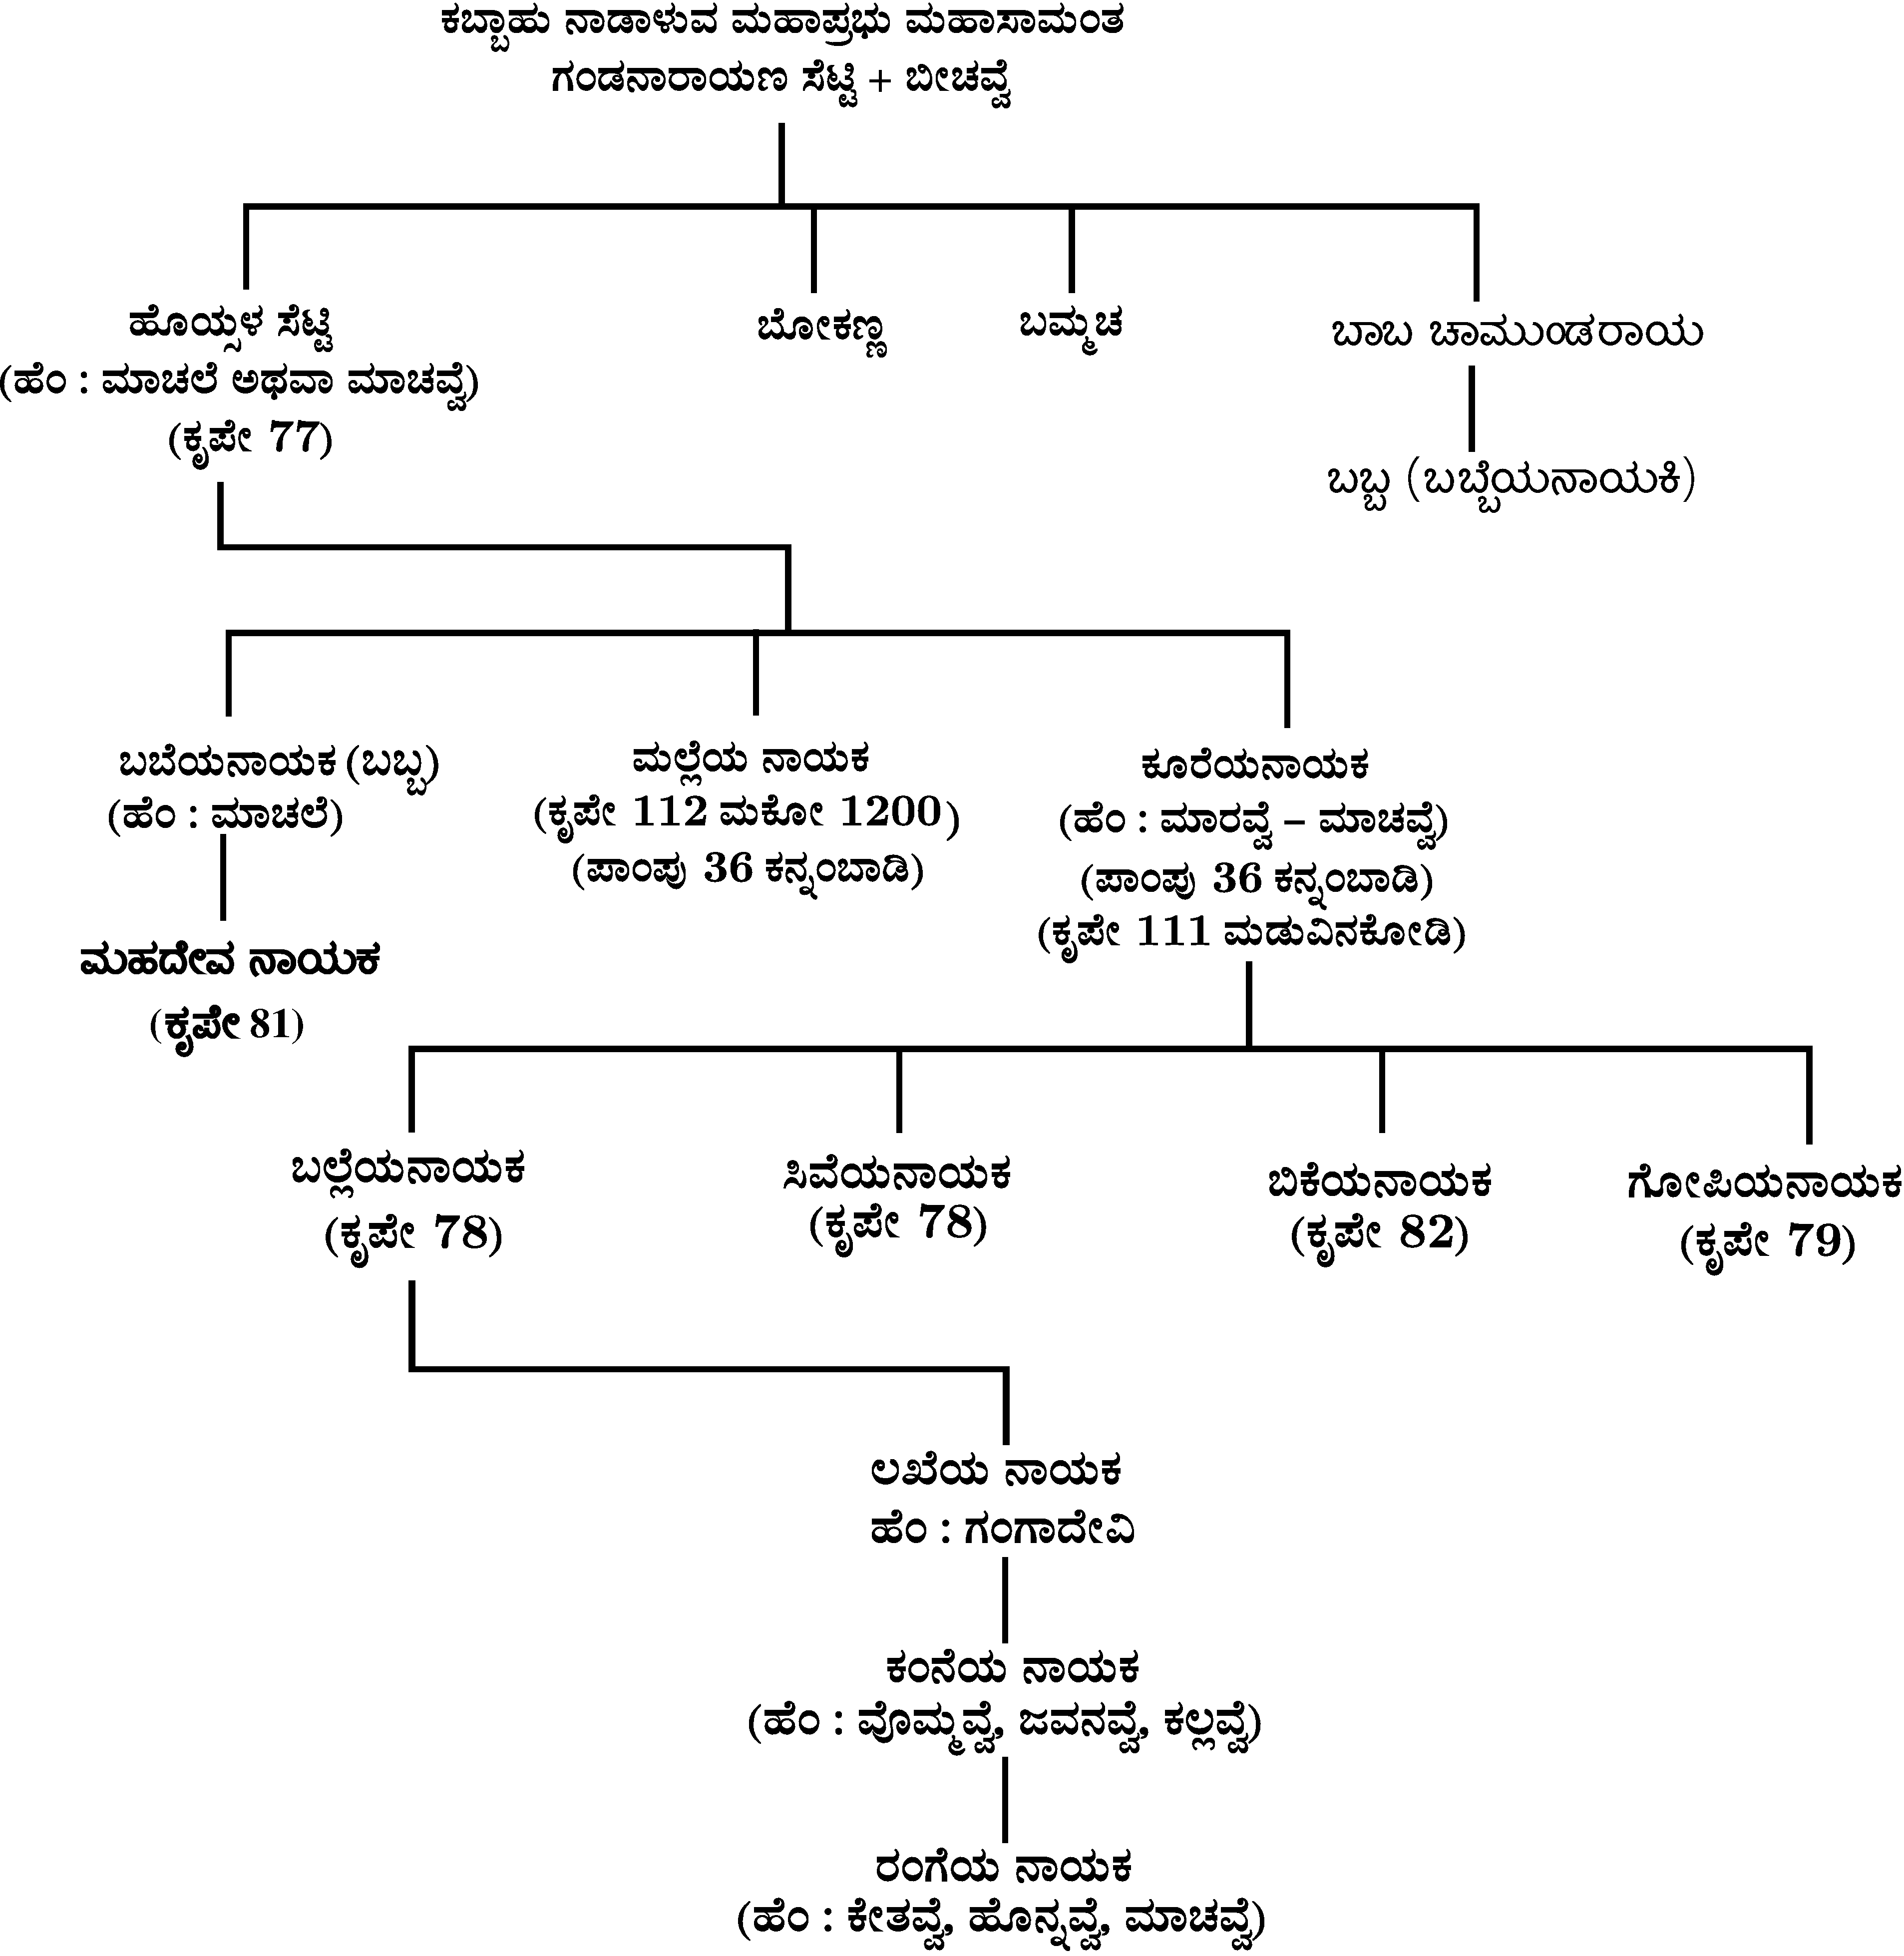
\includegraphics[scale=1]{images/chap3/chap3fig4.jpeg}
\end{figure}

\textbf{ಮಹಾಸಾಮಂತ\index{ಮಹಾಸಾಮಂತ} ಮಾಚೆಯನಾಯಕ\index{ಮಾಚೆಯ ನಾಯಕ}(1140):} ಮಹಾಸಾಮಂತ ಮಾಚೆಯನಾಯಕನು ವಿಷ್ಣುವರ್ಧನನ ಕಾಲದಲ್ಲಿ ಮಾಳಿಗೆಯೂರನ್ನು\index{ಮಾಳಿಗೆಯೂರು} ಆಳುತ್ತಿದ್ದ ಒಬ್ಬ ನಾಯಕನಿಗೆ ಅಳಿಯನಾಗಿದ್ದು, ಮಾಳಿಗೆಯೂರಿನ ವೃತ್ತಿಯನಾಯಕನಾಗಿದ್ದನೆಂದು ಹುಬ್ಬನಹಳ್ಳಿ ಶಾಸನದಲ್ಲಿ ಹೇಳಿದೆ.\endnote{ ಎಕ 6 ಕೃಪೇ 62 ಹುಬ್ಬನಹಳ್ಳಿ 1140} ಮಾಳಿಗೆಯೂರನ್ನು ಆಳುತ್ತಿದ್ದ ನಾಯಕನ ಹೆಸರು ತ್ರುಟಿತವಾಗಿದೆ. ಮಾಳಗೂರಿನ ಕ್ರಿ.ಶ.1117ರ ಶಾಸನದಲ್ಲಿ, ವಿಷ್ಣುವರ್ಧನನ ಪಿರಿಯರಸಿ ಪಟ್ಟಮಹಾದೇವಿ ಶಾಂತಲೆಯರ\index{ಪಟ್ಟಮಹಾದೇವಿ ಶಾಂತಲದೇವಿ} ಮೈದುನ ಶ‍್ರೀಮತು ಬಲ್ಲೆಯ\-ನಾಯಕನು\index{ಬಲ್ಲೆಯನಾಯಕ} ಮಾಳಿಗೆಯೂರನ್ನು ಆಳುತ್ತಿದ್ದನೆಂದು ಹೇಳಿದೆ.\endnote{ ಎಕ 6 ಕೃಪೇ 64 ಮಾಳಗೂರು 1117} ಬಲ್ಲೆಯನಾಯಕನು ಶಾಂತಲೆಯ ಸೋದರಮಾವ ನಾಗದೇವನ ಮಗ. ಈತ ಶಾಂತಲೆಗಿಂತ ಕಿರಿಯನಾದುದರಿಂದ ಮೈದುನ ಎಂದು ಹೇಳಿದೆ. ಬಲದೇವನು ಮೋರಿಂಗೆರೆಯ ತೀರ್ಥದಲ್ಲಿ ಮುಡಿಪಿ ಸ್ವರ್ಗಸ್ಥನಾದನೆಂದು ಶ್ರವಣಬೆಳಗೊಳದ ಕ್ರಿ.ಶ.1139\enginline{-}40ರ ಶಾಸನದಿಂದ ತಿಳಿದುಬರುತ್ತದೆ.\endnote{ ಎಕ 2 ಶ್ರಬೆ 174 ಚಿಕ್ಕಬೆಟ್ಟ 1139} ಬಲ್ಲೆಯನಾಯಕನ ನಂತರ ಅವನ ಅಳಿಯ ಮಾಚೆಯ ನಾಯಕನೇ\index{ಮಾಚೆಯ ನಾಯಕ} ಈ ಊರನ್ನು ಸಾಮಂತನಾಗಿ ಆಳುತ್ತಿದ್ದಿರಬಹುದು. ಬಲ್ಲೆಯನಾಯಕನು ಸನ್ಯಸನ ವಿಧಿಯಿಂದ ಮಡಿದಾಗ ಅವನ ತಾಯಿ ನಾಗಿಯಕ್ಕ\index{ನಾಗಿಯಕ್ಕ} ಅವನ ತಂಗಿ ಏಚಿಯಕ್ಕ\index{ಏಚಿಯಕ್ಕ} ಇವರು ಮಾಳಿಗೆಯೂರಿನಲ್ಲಿ (ಮಾಳಗೂರು) ಪಟ್ಟಸಾಲೆಯನ್ನು\index{ಪಟ್ಟಸಾಲೆ} ನಿರ್ಮಿಸಿ ಪ್ರಭಾಚಂದ್ರ ಸಿದ್ಧಾಂತ\index{ಪ್ರಭಾಚಂದ್ರ (ಸಿದ್ಧಾಂತ-ದೇವರು-ಸೈದ್ಧಾಂತಿಕ)} ದೇವರಿಗೆ ದತ್ತಿಯಾಗಿ ಬಿಡುತ್ತಾರೆ. ಕ್ರಿ.ಶ.1140ರ ಹುಬ್ಬನಹಳ್ಳಿ ಈ ಶಾಸನದ ಕಾಲ ಗಂಗರ ಕಾಲದ ಶಾಸನಕ್ಕೆ ಸರಿಹೊಂದುತ್ತದೆ. ಮಾಚೆಯನಾಯಕನ ತಾಯಿ ರಾಜೇಂದ್ರಚೋಳ ಹುಳ್ಳಗಾವುಂಡನ\index{ರಾಜೇಂದ್ರಚೋಳ ಹುಳ್ಳಗಾವುಂಡ} ಮಗಳಾಗಿದ್ದು, ಶಾಸನದಲ್ಲಿ ಇವಳ ಹೆಸರು ಅಳಿಸಿಹೋಗಿದೆ. ಮಾಚೆಯನಾಯಕನ ಹೆಂಡತಿ ಮೇಳಿ\index{ಮೇಳಿ}. ಇವರ ಮಗ ಒಡಗೆರೆಮಲ್ಲ.(ಇದೂ ಕೂಡಾ ಬಿರುದಿರಬಹುದು) ಈ ಒಡಗೆರೆ ಮಲ್ಲನು ಚೋಳತುರುನಾಡನ್ನು ಆಳುತ್ತಿದ್ದನು. ಈತನು ಅನ್ನ, ಸುವರ್ಣ, ಗೋದಾನ, ಭೂಮಿದಾನ, ಕನ್ಯಾದಾನಗಳನ್ನು ಮಾಡಿಸಿ, ಕೆರೆಯನ್ನು ಕಟ್ಟಿಸಿ, ಸಿವಾಲಯಗಳನ್ನು ನಿರ್ಮಿಸಿದನೆಂದು ಶಾಸನ ಹೇಳುತ್ತದೆ. ಅದೇ ರೀತಿ ಮಹಾಸಾಮಂತ ಮಾಚೆಯನು ಹುಬ್ಬನಹಳ್ಳಿಯಲ್ಲಿ\index{ಹುಬ್ಬನಹಳ್ಳಿ} ಹಿರಿಯ ಕೆರೆಯನ್ನು ಮಾಕೇಶ್ವರ ದೇವಾಲಯವನ್ನು\index{ಮಾಕೇಶ್ವರ ದೇವಾಲಯ} ನಿರ್ಮಿಸಿ, ಆ ದೇವರಿಗೆ ಭೂಮಿಯನ್ನು ದತ್ತಿಯಾಗಿ ಬಿಟ್ಟನು. ಶಾಸನದಲ್ಲಿ ನೇರಲಕೆರೆಯ\index{ನೇರಲಕೆರೆ} ಕೆಳಗೆ ಮಾಕೇಶ್ವರ ದೇವರಿಗೆ ದತ್ತಿ ಬಿಟ್ಟನೆಂದು ಹೇಳಿದ್ದು, ಈ ಊರಿನಲ್ಲಿ ಈಗಲೂ ಇರುವ ನೇರಲಕಟ್ಟೆ ಎಂಬ ಸಣ್ಣಕಟ್ಟೆಯಿದ್ದು, ಅದರ ಬಳಿಯೇ ಜೀರ್ಣವಾದ ದೇವಾಲಯ ಮತ್ತು ಶಾಸನ ಇದೆ.

ಶ್ರವಣ ಬೆಳಗೊಳ\index{ಶ್ರವಣಬೆಳಗೊಳ} ಮತ್ತು ಹುಬ್ಬನಹಳ್ಳಿ\index{ಹುಬ್ಬನಹಳ್ಳಿ} ಶಾಸನಗಳಿಂದ ಈ ಎರಡೂ ಮನೆತನಗಳ ವಂಶ ವೃಕ್ಷವನ್ನು ಈ ರೀತಿ ಕಟ್ಟಿ ಕೊಡಬಹುದು.
\begin{figure}[H]
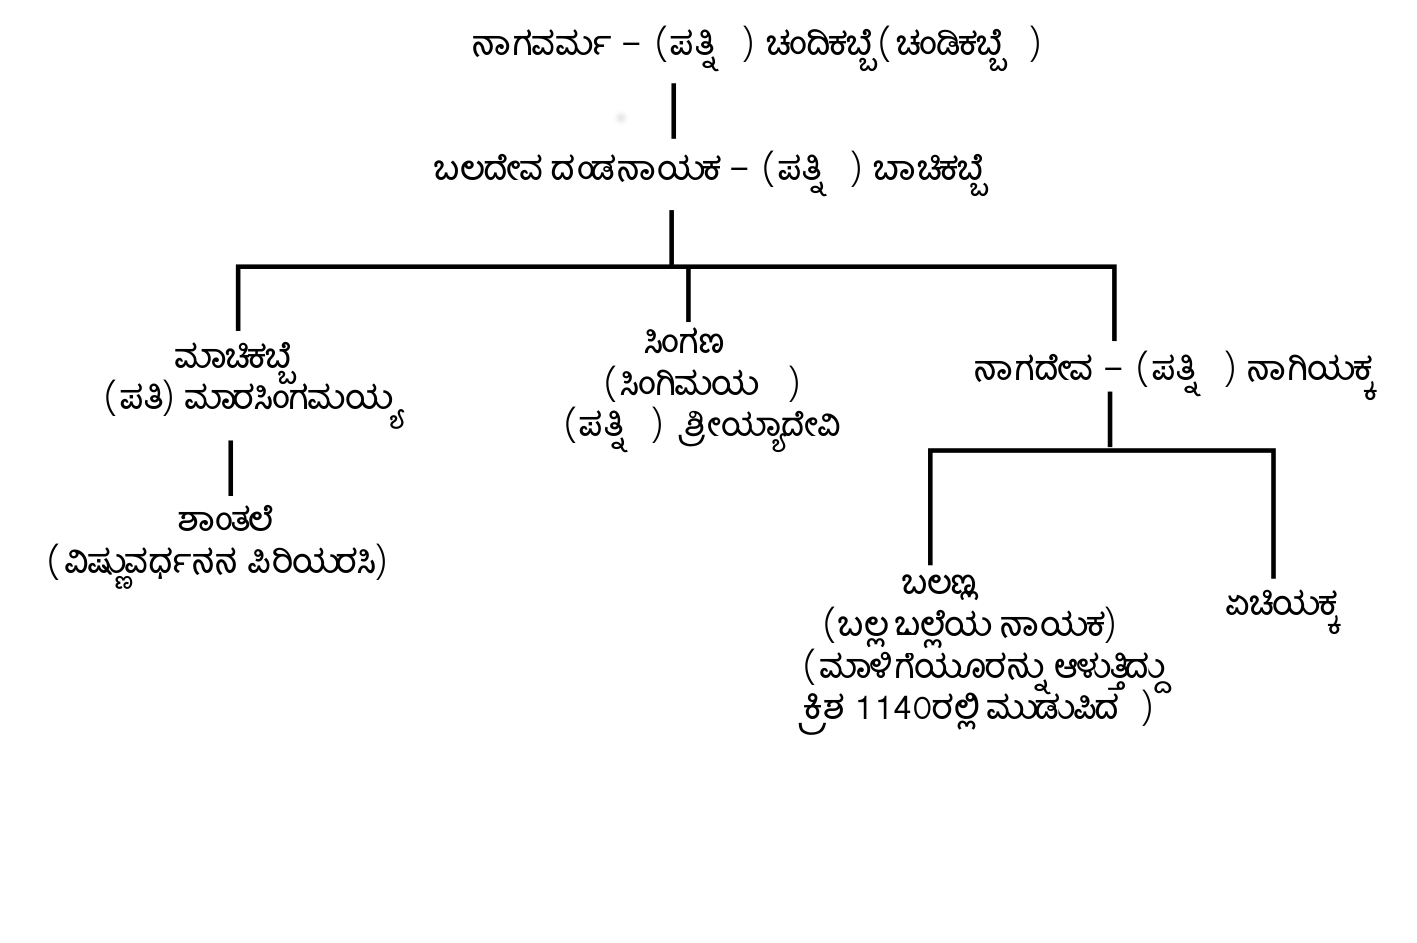
\includegraphics[scale=.24]{images/chap3/chap3fig4-1.jpeg}

\vskip -1.3cm

\centering{------------------------}

\vskip .6cm

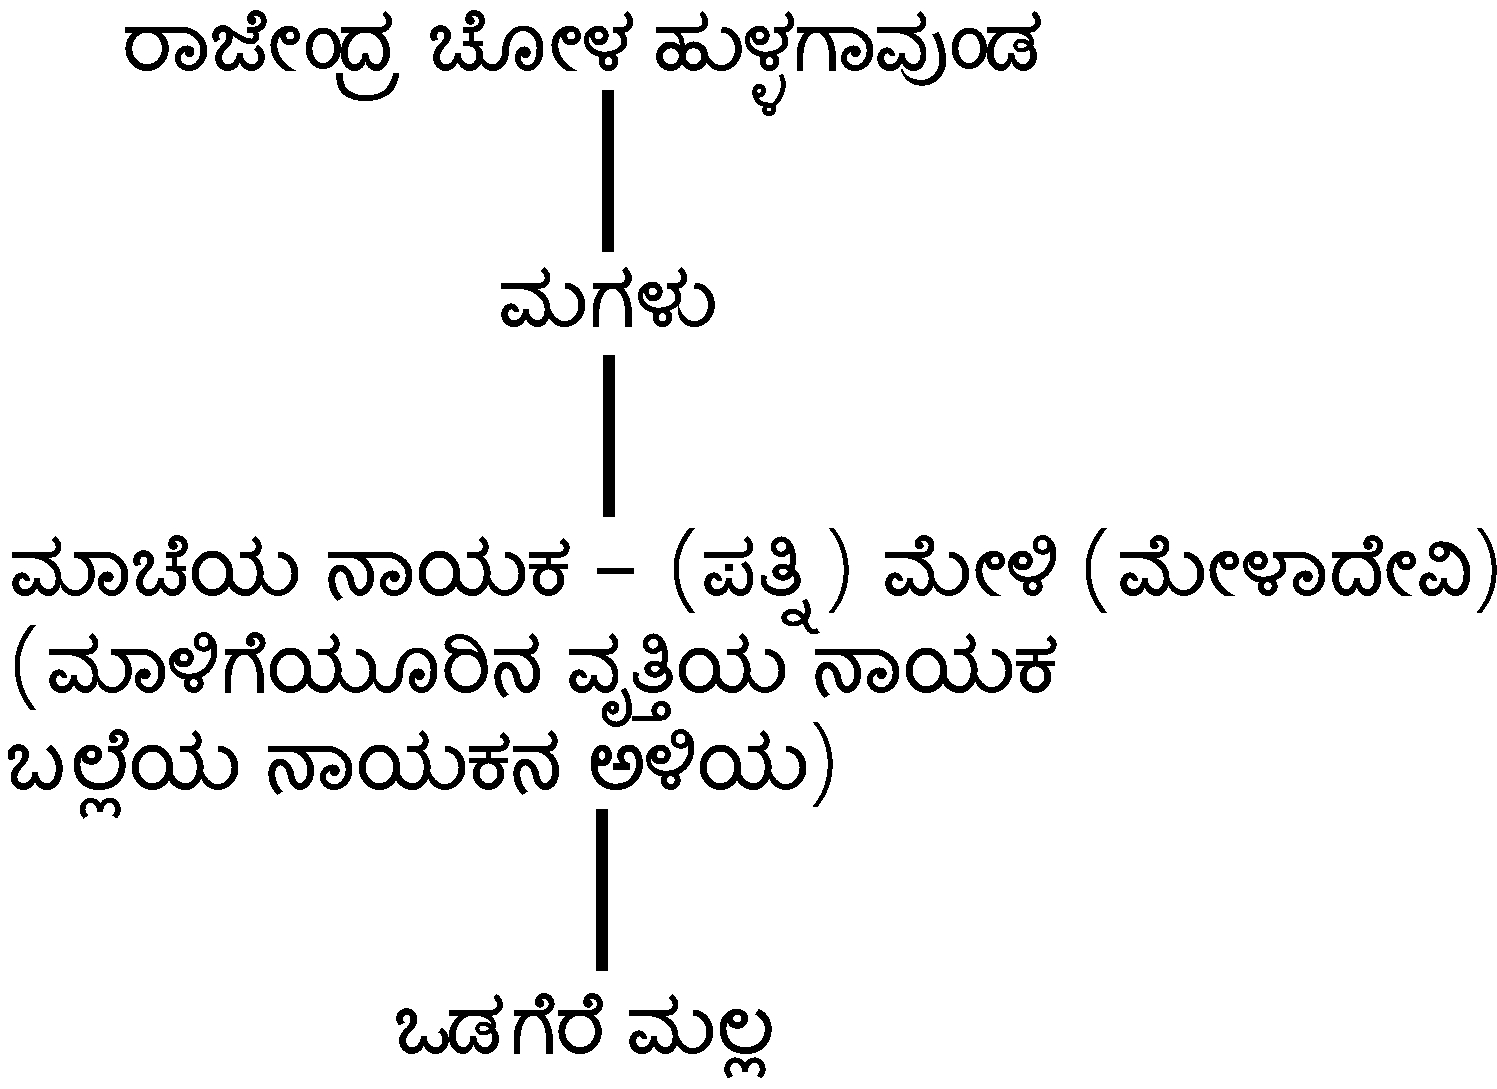
\includegraphics[scale=1.05]{images/chap3/chap3fig4.2.jpg}
\end{figure}

ಎಪಿಗ್ರಾಫಿಯಾ 2ರ ಸಂಪಾದಕರು ನಾಗದೇವನಿಗೆ ಬಲ್ಲ - ಬಲ್ಲೆಯ ನಾಯಕ ಎಂಬ ಇಬ್ಬರು ಮಕ್ಕಳಿದ್ದರೆಂದು ಹೇಳಿದ್ದಾರೆ. ಆದರೆ ಇಬ್ಬರೂ ಒಬ್ಬರೇ ಎಂಬುದು ಶಾಸನದ ಪರಿಶೀಲನೆಯಿಂದ ತಿಳಿದುಬರುತ್ತದೆ.\endnote{ (ಎಕ 2 ಪೀಠಿಕೆ ಪುಟ lviii)}

\textbf{ಸಾಮಂತ\index{ಸಾಮಂತ} ಭೀಮಣ್ಣ\index{ಭೀಮಣ್ಣ} ಮತ್ತು ಮಹಾಸಾಮಂತ ಬರ್ಮ್ಮಯ್ಯ\index{ಬರ್ಮ್ಮಯ್ಯ}(1171}): ವಿನಯಾದಿತ್ಯನ ಕಾಲದಲ್ಲಿ ಕಿಕ್ಕೇರಿಯನ್ನು ಆಳುತ್ತಿದ್ದ ಮೊನೆಯಾಳು\index{ಮೊನೆಯಾಳು} ಬಿಣ್ಣಮ್ಮನ\index{ಬಿಣ್ಣಮ್ಮ} ಮಗ ಸಾಮಂತ ಭೀಮಣ್ಣನು ಮೂಲಸ್ಥಾನ ಬ್ರಹ್ಮೇಶ್ವರ\index{ಮೂಲಸ್ಥಾನ ಬ್ರಹ್ಮೇಶ್ವರ} ದೇವರಿಗೆ ಕವುಂಗಿನ ತೋಟವನ್ನು\index{ಕವುಂಗಿನ ತೋಟ} ದತ್ತಿಬಿಟ್ಟನೆಂದು ತಿಳಿದುಬರುತ್ತದೆ.\endnote{ ಎಕ 6 ಕೃಪೇ 37 ಕಿಕ್ಕೇರಿ 1095-96} ವಿಷ್ಣುವರ್ಧನನ\index{ವಿಷ್ಣುವರ್ಧನ (ದೇವರು) (ಹೊಯ್ಸಳರ ದೊರೆ)} ಕಾಲದಲ್ಲಿ ಚಿಣ್ಣನು\index{ಚಿಣ್ಣ} ಕಿಕ್ಕೇರಿ ಪನ್ನೆರಡನ್ನು\index{ಕಿಕ್ಕೇರಿ ಪನ್ನೆರಡು(12)} ಆಳುತ್ತಿದ್ದನೆಂದು ಹೇಳಿದೆ.\endnote{ ಎಕ 6 ಕೃಪೇ 73 ಹಿರಿಕಳಲೆ 12ನೇ ಶ.} ಆದರೆ ಅವನು ಯಾವ ಅಧಿಕಾರದಿಂದ ಆಳುತ್ತಿದ್ದನು ಎಂಬುದನ್ನು ಹೇಳಿಲ್ಲ. ಚಿಣ್ಣನನ್ನು ಶಾಸನ ಬಹಳವಾಗಿ ಸ್ತುತಿಸಿದ್ದು ಈತ ಸಾಮಂತನೋ, ಮಹಾಸಾಮಂತನೋ ಆಗಿರುವ ಸಾಧ್ಯತೆ ಇದೆ.

\begin{verse}
\textbf{ದಾನಧರ್ಮ್ಮದ ಗುಣದಭಿ} \\\textbf{ಮಾನದ ಕಲಿತನದ ಚಲದ ಸತ್ಯದ ಪೆಂಪಿನ} \\\textbf{ಕಾನೀನನೆನಿಸಿ ನೆಗಳ್ದ} \\\textbf{ಮಾನವ ಜನ ಪೂಜ್ಯನಲ್ತೆ ಮೊನೆಯೊಳ್​ ಚಿಂಣ್ನಂ}
\end{verse}

\begin{verse}
\textbf{ಬಗೆಯೊಡೆ ಪತಿಹಿತದೆಯೊಳು} \\\textbf{ಖಗರಾಜನಿನೇಕದೊಡನಿಂ ಹನ್ಮನೆನೀ} \\\textbf{ಜಗದಾಳಮೊನೆಯೊಳು ಚಿಣ್ನಂ} \\\textbf{ದ್ವಿಗುಣಮತ್ರಿಗುಣಂಚತುರ್ಗಣಂ ಪಣ್ಯಾಗುಣಂ}
\end{verse}

ಮಹಾಸಾಮಂತ ಬರ್ಮ್ಮಯ್ಯನು ಒಂದನೆಯ ನರಸಿಂಹನ ಕಾಲದಲ್ಲಿ ಕಿಕ್ಕೇರಿಯನ್ನು ಆಳುತ್ತಿದ್ದನು. ಇವನನ್ನು ಶಾಸನವು \textbf{“ಸಮಸ್ತ ಪ್ರಶಸ್ತಿ ಸಹಿತಂ ಸಮಸ್ತ ನಾಮಾವಳಿಸಮಾಲಂಕೃತರುಂ ವೈರಿಸಾಮಂತ ದಿಶಾಪಟ್ಟನುಂ ಅರಿಬಿರುದರ ಸಾಮಂತ ಗಂಡಬೇರುಂಡ, ಗುಣಸಂಪನ್ನರಪ್ಪ ಶ‍್ರೀಮನ್​ ಮಹಾಸಾಮಂತ ಹುಲಿಯಜಂಗುಳಿ\index{ಹುಲಿಯ ಜಂಗುಳಿ} ಪ್ರಮುಖ ಮುಖ್ಯವಾದ ಸಾಮನ್ತ ಬರ್ಮಯ್ಯ” }ಎಂದು ವರ್ಣಿಸಿದೆ. ಹುಲಿಯ ಜಂಗುಳಿ ಎಂಬುದು ಒಂದು ರೀತಿಯ ಸೇನಾಪಡೆಯೆಂದೂ, ಅದಕ್ಕೆ ಈತನು ಮುಖ್ಯನಾಗಿದ್ದನೆಂದೂ ಹೇಳಬಹುದು. ಈತನ ಪತ್ನಿ ಬಮ್ಮವ್ವೆ ನಾಯಕಿತ್ತಿಯು\index{ಬಮ್ಮವ್ವೆ ನಾಯಕಿತ್ತಿ} ಕಿಕ್ಕೇರಿಪುರದಲ್ಲಿ\index{ಕಿಕ್ಕೇರಿಯ ಪುರ} ಬ್ರಹ್ಮೇಶ್ವರ ದೇವಾಲಯವನ್ನು\index{ಬ್ರಹ್ಮೇಶ್ವರ ದೇವಾಲಯ} ನಿರ್ಮಿಸಿದಳು.\endnote{ ಎಕ 6 ಕೃಪೆ 27 ಕಿಕ್ಕೇರಿ 1171 ಡಿಸೆಂಬರ್​ 23} ಇವರೆಲ್ಲರೂ ಒಂದೇ ವಂಶಕ್ಕೆ ಸೇರಿದ್ದು ವಂಶಪಾರಂಪರ್ಯವಾಗಿ ಕಿಕ್ಕೇರಿಯನ್ನು ಆಳುತ್ತಿದ್ದರೆಂದು ಹೇಳಬಹುದು. ಈ ಶಾಸನಗಳಿಂದ ಹೊರಡುವ ಇವರ ವಂಶಾವಳಿ ಈ ಕೆಳಗಿನಂತಿದೆ.

\begin{figure}[H]
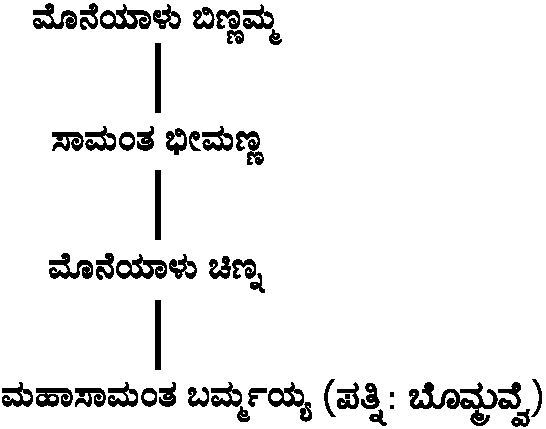
\includegraphics[scale=1.22]{images/chap3/chap3fig5.jpeg}
\end{figure}

\textbf{ಮಹಾಸಾಮಂತ\index{ಮಹಾಸಾಮಂತ} ದುಮ್ಮೆಯ ನಾಯಕ\index{ದುಮ್ಮೆಯ ನಾಯಕ} (12ನೇ ಶ.):} ಎರಡನೇ ಬಲ್ಲಾಳನ ಕಾಲದಲ್ಲಿ ಕಲಕುಣಿ ನಾಡನ್ನು ಆಳುತ್ತಿದ್ದ ಮಹಾಸಾಮಂತ ದುಮ್ಮೆಯ ನಾಯಕನ ವಂಶಾವಳಿ ಹಾಗೂ ಸಾಧನೆಗಳನ್ನು, ದೊಡ್ಡಜಟಕಾ\index{ದೊಡ್ಡಜಟಕಾ} ಶಾಸನವು ವಿವರವಾಗಿ ನೀಡುತ್ತದೆ.\endnote{ ಎಕ 7 ನಾಮಂ 132 ದೊಡ್ಡಜಟಕಾ} ಇವರು ಮೊದಲಿಗೆ ಸೆಟ್ಟಿ ಅಂದರೆ ವರ್ತಕ ಸಮುದಾಯದವರಾಗಿ, ಜೈನಧರ್ಮದ ಅನುಯಾಯಿಗಳಾಗಿದ್ದು, ದುಮ್ಮೆಯ\-ನಾಯಕನ ಕಾಲಕ್ಕೆ ಶೈವಧರ್ಮವನ್ನು ಸ್ವೀಕರಿಸಿದ್ದರೆಂದು ಹೇಳಬಹುದು. ಈ ವಂಶದ ಮೂಲ ಪುರುಷ ಮಾರಸಿಂಗ ಗಾವುಂಡನು\index{ಮಾರಸಿಂಗ ಗಾವುಂಡ} ತಲಕಾಡು ನಾಡನ್ನು ಆಳುತ್ತಿದ್ದ. ಇವನ ಮಗ ಪುರುಷಮಾಣಿಕ್ಯ ಸೆಟ್ಟಿಯು\index{ಪುರುಷಮಾಣಿಕ್ಯ ಸೆಟ್ಟಿ}, ಸಮಯ(ಜೈನಧರ್ಮ) ಮತ್ತು ತಲಕಾಡು ಪಟ್ಟಣ\index{ತಲಕಾಡು ಪಟ್ಟಣ} ಎರಡನ್ನೂ ಸಮುದ್ಧರಣ ಮಾಡಿದನು. ಈ ವಂಶದವರ ಸೇವೆಯನ್ನು ಗಮನಿಸಿ ಹುಳ್ಳೆಯ ನಾಯಕನನ್ನು\index{ಹುಳ್ಳೆಯ ನಾಯಕ} ಮೊದಲಿಗೆ ಕಲಕುಣಿ ನಾಡಿನ ಮಹಾಸಾಮಂತನನ್ನಾಗಿ ನೇಮಕ ಮಾಡಿರಬಹುದು. ಸಾಮಂತರನ್ನು ಬೇರೆಬೇರೆ ಪ್ರಾಂತಗಳಿಗೆ ವರ್ಗಾಯಿಸಿ ನೇಮಿಸಲಾಗುತ್ತಿತ್ತು ಎಂದು ಇದರಿಂದ ತಿಳಿದುಬರುತ್ತದೆ.

ಹುಳ್ಳೆಯ ನಾಯಕನು ಜಟ್ಟಿಗವನ್ನು ಊರನ್ನಾಗಿ ಮಾಡಿ ಕೆರೆಯನ್ನು ಕಟ್ಟಿಸಿ ಉದ್ಯೋಗ ಮಲ್ಲನೆನಿಸಿದನು\index{ಉದ್ಯೋಗ ಮಲ್ಲ}. ಇವನ ಮಗ ಮಹಾ ಸಾಮಂತ ಹೆಮ್ಮೆಯ ನಾಯಕನನ್ನು\index{ಹೆಮ್ಮೆಯ ನಾಯಕ} ಶಾಸನವು \textbf{“ಸಮಸ್ತ ಗುಣಸಂಪಂನ್ನ ಆಹಾರಾಭಯ ಸಾಸ್ತ್ರವಿನೋದನುಂ ಜಿನಸಮಯ ಸಮುದ್ಧರಣಂ ಪಾರೀಷದೇವರ ಪಾದಾರಾಧಕನುಂ ಬಂಟರಭಾವನುಂ ನಂಟರಂಗರಕನುಂ ಒಡಗೆರೆಮಲ್ಲನುಂ ಕೂಡಿತಪ್ಪುನಾಯಕರಗಂಡ ನುಡಿದಂನ್ತೆ ಗಂಡ ಮಾರ್ಕ್ಕೋಲಭೈರವಂ ಮಾಹಾಸಾಮನ್ತ ಹೆಮ್ಮೆಯ ನಾಯಕಂ”} ಎಂದು ವರ್ಣಿಸಿದೆ.

ಇವನ ಮಗನೇ ಧುರ್ಮ್ಮಣ್ಣ\index{ಧುರ್ಮ್ಮಣ್ಣ} ಅಥವಾ ದುಮ್ಮೆಯ ನಾಯಕ\index{ದುಮ್ಮೆಯ ನಾಯಕ}. \textbf{ಹರಿಹರಬ್ರಹ್ಮಾದಿಗಳೇ ಬಂದು ಇವನನ್ನು ಹರಸಿ ಪಟ್ಟಕಟ್ಟಿದ\-ರೆಂದು,} ಶಾಸನವು ಇವನನ್ನು ವಿಶೇಷವಾಗಿ ವರ್ಣಿಸಿದೆ.\textbf{ “ಆತನ ಕೀರ್ತ್ಯಾವತಾರವೆನ್ತೆಂದಡೆ ಸ್ವಸ್ತಿ ಶ‍್ರೀಮತು\general{\break } ಚತುಸಮಯಸಮುದ್ಧರಣಂ ಧರಣಿದೇವತಾರುದ್ರನುಂ। ಆಹಾರಾಭಯನುಂ। ಗೋತ್ರಪವಿತ್ರನುಂ~।ಬಂಟರಬಾವನುಂ।\general{\break } ನಂಟರಂಗರಕನುಂ~।ನುಡಿದಂನ್ತೆಗಂಡನುಂ। ಚಲಕೆಬಲುಗಂಡ। ತಪ್ಪೆತಪ್ಪುವಂ ತನದಟ್ಟಿಬಡಿವಂ। ಮಗುರ್ದಡೆರೆಪ್ಪುವ। ಕೂಡಿತಪ್ಪುವ ನಾಯಕರಗಂಡ। ಕನ್ನೆಗೆರೆಮಲ್ಲ। ಮಚ್ಚರಿಪನಾಯಕರಗಂಣ್ಡ ತೊಡರ್ದ್ದರಂಕುಸ ಗಾಂನ್ಧವರಾನೆ ಹೊಯ್ಸಳ ಮಹಾಸಾಮಂನ್ತ\general{\break } ದುಮ್ಮೆಯನಾಯಕರು।”} ಎಂದು ಸಾಂಪ್ರದಾಯಿಕವಾಗಿ ವರ್ಣಿಸಲಾಗಿದೆ. ದುಮ್ಮೆಯ ನಾಯಕನು ಕಲ್ಕಣಿನಾಡ ಜೆಟ್ಟಿಗದ ಹೇಮೇಸ್ವರ ದೇವರ ದೇವಾಲಯವನ್ನು\index{ಜೆಟ್ಟಿಗದ ಹೇಮೇಸ್ವರ ದೇವಾಲಯ} ಕಟ್ಟಿಸಿ ಕಳಸ ನಿರ್ವಾಣಗೆಯ್ಸಿ ಆ ದೇವರ ಪೂಜಿಸುವ ಬಾಚಜೀಯಂಗೆ\index{ಬಾಚಜೀಯ} ದತ್ತಿಗಳನ್ನು ಬಿಡುತ್ತಾನೆ. ಅಲ್ಲೇ ಇರುವ ಇನ್ನೊಂದು ತ್ರುಟಿತ ಶಾಸನ ದುಮ್ಮೆಯ ನಾಯಕನ ಪ್ರಶಸ್ತಿ ಶಾಸನವಾಗಿದೆ.\endnote{ ಎಕ 7 ನಾಮಂ 131 ದೊಡ್ಡಜಟಕ} ಹೆಮ್ಮಣ್ಣ ನಾಯಕನ ಹೆಂಡತಿ ತಿರುವವ್ವೆ ಎಂಬುದು ಅಲ್ಲೇ ಇರುವ ಇನ್ನೊಂದು ಶಾಸನದಿಂದ ತಿಳಿದುಬರುತ್ತದೆ.\endnote{ ಎಕ 7 ನಾಮಂ 130 ದೊಡ್ಡಜಟಕ 1179} ಈ ಶಾಸನಗಳಿಂದ ಇವರ ವಂಶಾವಳಿಯನ್ನು ಈ ರೀತಿ ಕಟ್ಟಿಕೊಡಬಹುದು.

\begin{figure}[H]
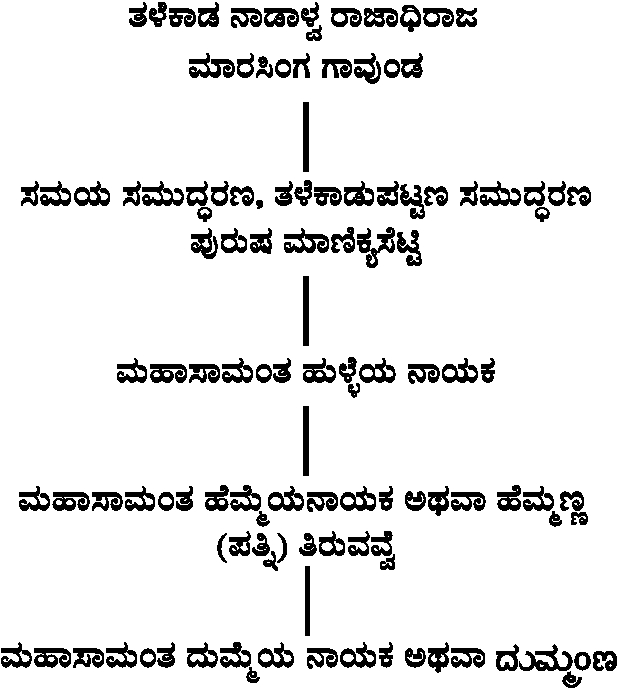
\includegraphics[scale=1.2]{images/chap3/chap3fig6.jpeg}
\end{figure}

\textbf{ಮಹಾಸಾಮಂತ\index{ಮಹಾಸಾಮಂತ} ದೇಕೆಯನಾಯಕ\index{ದೇಕೆಯ ನಾಯಕ}(1180):} ಇಮ್ಮಡಿ ಬಲ್ಲಾಳನ ಕಾಲದಲ್ಲಿ ಸಾಮಂತ ದೇಕೆಯ ನಾಯಕನು ಮೇಲಾಳಿಕೆ\-ಯನ್ನು\index{ಮೇಲಾಳಿಕೆ} ನಡೆಸುತ್ತಿದ್ದನೆಂದು ಹೊನ್ನೇನಹಳ್ಳಿ ಶಾಸನದಿಂದ ತಿಳಿದುಬರುತ್ತದೆ.\endnote{ ಎಕ 7 ನಾಮಂ 106 ಹೊನ್ನೇನಹಳ್ಳಿ 1180} ಯಾವ ನಾಡಿನ ಮೇಲೆ ಈತನ ಮೇಲಾಳಿಕೆ ಇತ್ತೆಂದು ತಿಳಿದುಬರುವುದಿಲ್ಲ. ಈತನನ್ನು ಶಾಸನವು \textbf{“ಸ್ವಸ್ತಿ ಸಮಸ್ತ ಪ್ರಶಸ್ತಿ ಸಹಿತಂ ಶ‍್ರೀಮನ್ಮಹಾಸಾಮಂತ ಎಸುವರಾದಿತ್ಯ\index{ಎಸುವರಾದಿತ್ಯ} ಕಣ್ನಂಬಿನೊಡೆಯ\index{ಕಣ್ನಂಬಿನೊಡೆಯ} ಸೈಗೋಲಮಾತ್ಯ ಬಂಟರಭಾವ ದಾಯಿಗಬೇಂಟೆಕಾರ ಶ‍್ರೀ ನೀಲಕಂಠ ದೇವರ\general{\break } ಪಾದಪದ್ಮಾರಾಧಕರುಮಪ್ಪ ಕುನ್ನಿಯ ಬೀರೆಯನಾಯಕನ\index{ಕುನ್ನಿಯ ಬೀರೆಯನಾಯಕ} ಮಗಂ ಸಾಮಂತ ದೇಕೆಯ ನಾಯಕ\index{ದೇಕೆಯ ನಾಯಕ}”} ಎಂದು ವರ್ಣಿಸಿದೆ. ಇವನ ಕಾಲದಲ್ಲಿ ಹಡವಳದ ಹೊನ್ನಯ್ಯ\index{ಹಡವಳದ ಹೊನ್ನಯ್ಯ} ಮತ್ತು ಅವನ ಭಾರ್ಯೆ ದೇಗುಲ ಗೌಣ್ಡಿ\index{ದೇಗುಲ ಗೌಣ್ಡಿ} ಇವರ ಮಗ ಹೊನ್ನೆಗೌಡನು ತುರುಗೋಳಿನಲ್ಲಿ ಮಡಿದ\-ನೆಂದಿದೆ. \textbf{ಎಸುವರಾದಿತ್ಯ ಮತ್ತು ಕಣ್ನಂಬಿನೊಡೆಯ ಎಂಬ ಬಿರುದುಗಳಿಂದ ಇವನು ಬಿಲ್ವಿದ್ಯೆಯಲ್ಲಿ ಪ್ರವೀಣ\-ನಾಗಿದ್ದನೆಂದು ಹೇಳಬಹುದು.}

\textbf{ಮಹಾಸಾಮಂತ\index{ಮಹಾಸಾಮಂತ} ಕಾಚೀದೇವ\index{ಕಾಚೀದೇವ} (1224):} ಮಹಾಸಾಮಂತ ಕಾಚೀ ದೇವನ ವಂಶಾವಳಿ ಹಾಗೂ ಸಾಧನೆಗಳನ್ನು ಬೆಳ್ಳೂರಿನ\index{ಬೆಳ್ಳೂರು} ದೀರ್ಘವಾದ ಶಾಸನ ನೀಡುತ್ತದೆ.\endnote{ ಎಕ 7 ನಾಮಂ 81 ಬೆಳ್ಳೂರು 1223-24} ಕುರುಭೂಮಿಯಲ್ಲಿ ಜನಿಸಿ ಬಂದ ಕುರುವಂದ ಕುಲಕ್ಕೆ\index{ಕುರುವಂದ ಕುಲ} ತಾವು ಸೇರಿದವರೆಂದು ಈ ವಂಶಸ್ಥರು ಹೇಳಿಕೊಂಡಿದ್ದಾರೆ. ವೀರರಾಜೇಂದ್ರಹೊಯ್ಸಳ ಮೊರಸಾಧಿರಾಯರೆಂದು\index{ಮೊರಸಾಧಿರಾಯ} ತಮ್ಮನ್ನು ಕರೆದುಕೊಂಡಿರುವುದರಿಂದ ಇವರು ಚೋಳರು ಅಥವಾ ಅವರ ಸಾಮಂತರಾಗಿದ್ದ ಚೆಂಗಾಳ್ವರ ವಂಶಸ್ಥರೋ ಅಥವಾ ಅವರ ಅಧೀನದಲ್ಲಿದ್ದ ಸಾಮಂತರೋ ಆಗಿರಬಹುದು. ಮೊರಸಾಧಿರಾಯ ಎಂದರೆ ಇವರು ಮೊರಸು ಕುಲಕ್ಕೆ\index{ಮೊರಸು ಕುಲ} ಸೇರಿದವರಾಗಿರಬಹುದೆಂದೂ ಊಹಿಸಬಹುದು. ಕಾರಣ ಬೆಂಗಳೂರು ಜಿಲ್ಲೆಯು ಬಹುಕಾಲ ಚೋಳರ ಅಧೀನದಲ್ಲಿತ್ತು ಹಾಗೂ ಅದನ್ನು ಮೊರಸುನಾಡು ಎಂದೂ ಕರೆಯಲಾಗು\-ತ್ತಿತ್ತು. ಈ ಭಾಗದಿಂದ ಇವರು ಬಂದವರಾಗಿದ್ದು, ವೀರರಾಜೇಂದ್ರ ಮೊರಸಾಧಿರಾಯರೆಂದು ಎಂದು ತಮ್ಮನ್ನು ಕರೆದುಕೊಂಡಿರು\-ವುದರಲ್ಲಿ ಅರ್ಥವಿದೆ. ಇದರಿಂದ ಮೊರಸು ಕುಲ\index{ಮೊರಸು ಕುಲ} ಮತ್ತು ಕುರುವಂದಕುಲ ಒಂದೇ ಎಂದು ತೋರುತ್ತದೆ.

ಈ ವಂಶದ ಮೂಲಪುರುಷ ಕುರುನಂದನರ ವಂಶದಲ್ಲಿ ಜನಿಸಿದ ನನ್ನಿಯ ಮೇರು\index{ನನ್ನಿಯ ಮೇರು}. ಈತನು ಕುರುಭೂಮಿಯಲ್ಲಿ ಜನಿಸಿಬಂದು, \textbf{“ಹೊಯ್ಸಳಖ್ಯಾತರಂ ಪದುಳಂ ಮಾಡಿ”} ಎಂದರೆ ಹೊಯ್ಸಳ ರಾಜರನ್ನು ಒಲಿಸಿ ಮತ್ತು ಅವರ ರಾಜ್ಯವನ್ನು ತನ್ನ ಜನ್ಮಕ್ಷೇತ್ರವನ್ನಾಗಿ ಮಾಡಿಕೊಂಡು \textbf{“ಎಡಗೈಯ ಮೊತ್ತದ ಸೇನಾನಾಯಕ\index{ಎಡಗೆಯ್ಯ (ಮೊತ್ತದ) ಸೇನಾನಾಯಕ}}”ನೆನಿಸಿದನು. ಚೋಳರು ಅಥವಾ ಚೆಂಗಾಳ್ವರ ಪತನದ ನಂತರ ಇವರು ಹೊಯ್ಸಳರನ್ನು ಆಶ್ರಯಿಸಿದರೆಂದು ಹೇಳಬಹುದು. ನಂನಿಯಮೇರು ಚತುರ್ತ್ಥ ವಂಶರೊಳು ರಣಿತಗವುಂಡನುದ್ಭವಿಸಿ” ಅಂದರೆ ನನ್ನಿಯ ಮೇರುವಿನ ಮಗ ರಣಿತಗವುಂಡ\index{ರಣಿತಗವುಂಡ}. ಚತುರ್ತ್ಥ ವಂಶರು\index{ಚತುರ್ತ್ಥ ವಂಶರು} ಎಂದರೆ ಚಾತುರ್ವರ್ಣದಲ್ಲಿ ನಾಲ್ಕನೆಯ ವರ್ಣದವರಾದ ಶೂದ್ರರು ಅಥವಾ ಗವುಡರು ಎಂಬುದು ಇದರಿಂದ ಅರ್ಥವಾಗುತ್ತದೆ. ರಣಿತ ಗವುಂಡನು ಹೊಯ್ಸಳರು ಹೂಡಿದ ಯುದ್ಧಗಳಲ್ಲಿ ಭಾಗವಹಿಸಿ ಶತ್ರು ರಾಜರನ್ನು ತವಿಸಿದನು. ರಣಿತ ಗವುಂಡನ ಮಗ ಸಿಂಗಾಡಿ ನಾಯಕ\index{ಸಿಂಗಾಡಿ ನಾಯಕ}. ಇವನು ಕಾಮದೇವನ ಮಿತ್ರನಂತಿದ್ದನು. ಇವನಿಗೆ ಅನಿರುದ್ಧನಂತಹ ಸಿಂಗಾಡಿ ದೇವನೆಂಬ\index{ಸಿಂಗಾಡಿ ದೇವ} ಮಗನು ಜನಿಸಿದನು. ಇವನನ್ನು ಸಾಮಂತ ಸಿಂಗಾಡಿ ದೇವನೆಂದು ಶಾಸನದಲ್ಲಿ ಹೇಳಿದ್ದು, ಬಹುಶಃ ಇವನ ಕಾಲದಿಂದ ಇವರು ಸಾಮಂತ ಪದವಿಗೆ ಏರಿದರೆಂದು ಹೇಳಬಹುದು. ಸಿಂಗಾಡಿ ದೇವನ ಮಗ ಹಿರಿಯ ಮಾಚ\index{ಮಾಚ}. ಇವನೂ ಖ್ಯಾತ ಸಾಮಂತನಾಗಿದ್ದನು. ಈತನ ಮಗ ವೀರ ಸಾಮಂತನೆನಿಸಿದ ಸಿಂಧ. ಇವನು ಹಟ್ಟಿಗಾಳೆಗದಲ್ಲಿ\index{ಹಟ್ಟಿಗಾಳೆಗ} ಪ್ರಸಿದ್ಧನಾಗಿದ್ದನು. ಸಿಂಧೆಯ ನಾಯಕನಿಗೆ\index{ಸಿಂಧೆಯ ನಾಯಕ}, ಮಾಚಿದೇವ, ವೀರನಾಯಕ, ವಿಭು ಬಲ್ಲಯ್ಯ ನಾಯಕ ಮತ್ತು ಹರಿಯಣ್ಣ ಎಂಬ ನಾಲ್ಕು ಜನ ಪುತ್ರರು. ಇವರಲ್ಲಿ ಮಾಚಿ ದೇವನು ಪ್ರಸಿದ್ಧನಾದನು. ಇವನ ಪತ್ನಿ ಬಮ್ಮಲದೇವಿ\index{ಬಮ್ಮಲದೇವಿ}. ಇವರಿಗೆ ಮಾಚೆಯನಾಯಕನೆಂಬ\index{ಮಾಚೆಯ ನಾಯಕ} ಮಗ. ಕುರುವಂದ ಕುಲೈಕಭೂಷಣನೆನಿಸಿದ ಮಾಚೆಯನಾಯಕನ ಹೆಂಡತಿಯರು ಬೇಡವ್ವೆ\index{ಬೇಡವ್ವೆ} ಮತ್ತು ಚೋಕಲದೇವಿ\index{ಚೋಕಲದೇವಿ}. ಬೇಡವ್ವೆಯ ಮಗ ಮಾಧವ\index{ಮಾಧವ}. ಚೋಕಲದೇವಿಗೆ ಕಾಚಿದೇವ, ಮಲ್ಲೆಯನಾಯಕ\index{ಮಲ್ಲೆಯ ನಾಯಕ} ಮತ್ತು ಬಲ್ಲಯ್ಯ\index{ಬಲ್ಲಯ್ಯ} ಎಂಬ ಮೂರು ಜನ ಮಕ್ಕಳು. ಬಲ್ಲೆಯನಾಯಕನ ಹೆಂಡತಿಯ ಹೆಸರು ಮಾಕಲೆ\index{ಮಾಕಲೆ}. ಬಲ್ಲಯ್ಯ ಮಾಕಲೆಯರ ಮಗನೇ ಸಿರಿರಂಗ ನಾಯಕ\index{ಸಿರಿರಂಗ ನಾಯಕ}. ಇವನ ಹೆಸರಿನಲ್ಲೇ ಬೆಳ್ಳೂರಿನ ಬಳಿಯ ಶ‍್ರೀರಂಗಪುರ ಅಗ್ರಹಾರವನ್ನು\index{ಶ‍್ರೀರಂಗಪುರ ಅಗ್ರಹಾರ} ಮಾಡಲಾಯಿತೆಂದು ಎಂದು ಹೇಳಬಹುದು. ಸಿರಿರಂಗ ನಾಯಕನ ಹೆಂಡತಿ ಮಲ್ಲಾಂಬಿಕೆ\index{ಮಲ್ಲಾಂಬಿಕೆ}. ಇವರಿಗೆ ಹರಿಯಣ್ಣ (ಹರ್ಯಣ), ಬಲ್ಲಾಳ, ಮಾಚಿದೇವ ಎಂಬ ಮೂವರು ಮಕ್ಕಳು. ಮಾಚೀ ದೇವನ ಹೆಂಡತಿ ಚೋಕವ್ವೆ ನಾಯಕಿತ್ತಿ. ಮಾಚಿದೇವ ಮತ್ತು ಚೋಕವ್ವೆ ನಾಯಕಿತ್ತಿಯರ ಮಗ ಕಾಚಿದೇವ. ಕಾಚಿದೇವನ ಪತ್ನಿ ಮಾಚಲರಾಣಿ\index{ಮಾಚಲರಾಣಿ}. ಇವರಿಗೆ ಲಕ್ಷ್ಮೀಕಾಂತ, ಮಾಚಿದೇವ ಮತ್ತು ಗೋಪಾಳ ಎಂಬ ಮೂರುಜನ ಮಕ್ಕಳು. ಮಹಾಸಾಮಂತ ಕಾಚೀದೇವನ ಹೆಸರಿನಲ್ಲಿಯೇ ಈ ಶಾಸನವು ಹೊರಟಿದೆ.

ಕಾಚಿದೇವನು ಸಾಮಂತ ಕಂಠೀರವನೆನಿಸಿ\index{ಸಾಮಂತ ಕಂಠೀರವ} ಪ್ರಖ್ಯಾತನಾದನು. ಶಾಸನವು ಕಾಚೀದೇವನನ್ನು, \textbf{“ಶ‍್ರೀಮನು ಮಹಾಸಾಮಂತ ಭುಜಬಳ ವೀರರಾಜೇಂದ್ರ ಹೊಯ್ಸಳ ಮೊರಸಾಧಿರಾಯ, ಮೂರುಲೋಕಜಗದಳಂ, ಕುರುವಂದ ಕುಲ ಕಮಲ\-ಮಾರ್ತಾಂಡ, ಹಟ್ಟಿಗಾಳೆಗಕ್ಕೆಕ ಮಲೆವ ಸಾಮಂತರಗಂಡ, ಪ್ರತಾಪಕಂಠೀರವ, ಪರಬಳಜಳಧಿಬಡಬಾನಳಂ, ಯಾದವರಾಜ್ಯ\-ಲಕ್ಷ್ಮೀ ಮುಖಸುರರತ್ನದರ್ಪ್ಪಣಂ ಶ‍್ರೀ ಚೆನ್ನಕೇಶವಪದಾಂಭೋಜಕಮಳಿನೀಕಳಹಂಸಭಿನವಪ್ರಹರಾಜ ಅದ್ಯತನ ಬಲೀಂದ್ರ, ಆ ಪುರಾಣ ಗಾಂಗೇಯ ಅಪರಿಮಿತದಾನಸಾರವೃಷ್ಟಿ, ಗೋಬ್ರಾಹ್ಮಣಹಯ ಧೂಳಿಧೂಸರ ಪವಿತ್ರೀಕ್ರಿತೋತ್ತಮಾಂಗ\general{\break } ಸಕಳಕಳಾವಿಧಾನ ಪದ್ಮಾಸನ ವಿದ್ವಜನವಿಪದಳನ ಚತುಷಷ್ಟಿಕಳಾಕಳಿತ ಸರ್ವಜ್ಞನಪರಿಮಿತದಾನವಿನೋದಶೀಳ ಎಡಗೈಯ್ಯ\general{\break } ಸೇನಾನಾಯಕ ಕಾಚೀದೇವ}”ನೆಂದು ವರ್ಣಿಸಿದೆ. ಕಾಚೀ ದೇವನು ಕಲ್ಕಣಿನಾಡ\index{ಕಲುಕಣಿ (ಕಲಿಕಣಿ-ಕಲ್ಕಣಿ-ಕಲ್ಕುಣಿ-ಕಲುಕರೆ) ನಾಡು} ಬೆಳ್ಳೂರ ಸ್ಥಳದಲು\index{ಬೆಳ್ಳೂರು ಸ್ಥಳ} ಶ‍್ರೀ ಸಿಂಧೇಶ್ವರ\index{ಸಿಂಧೇಶ್ವರ}, ಲಕ್ಷ್ಮೀನಾರಾಯಣ\index{ಲಕ್ಷ್ಮೀನಾರಾಯಣ}, ಗೋಪಾಳದೇವರ\index{ಗೋಪಾಳದೇವರು} ತ್ರಿಕೂಟ ದೇವಾಲಯವನ್ನು ನಿರ್ಮಿಸಿ, ದೇವರ ಪ್ರತಿಷ್ಠೆಯನ್ನು ಮಾಡಿ, ಆ ದೇವರ ಅಂಗಭೋಗ, ರಂಗಭೋಗ, ಖಂಡಸ್ಫುಟಿತ ಜೀರ್ಣೋದ್ಧಾರಕ್ಕೆ ಅಷ್ಟವಿಧಾರ್ಚನೆಗೆ, ಮಠಪತಿದಾಸ\index{ಮಠಪತಿದಾಸ} ವೈಷ್ಣವರ\index{ವೈಷ್ಣವರು} ಆಹಾರ ದಾನಕ್ಕೆ ದತ್ತಿಯನ್ನು ಬಿಡುತ್ತಾನೆ. ಶಾಸನದಲ್ಲಿ ಹೇಳಿರುವ ಮಾಚಸಮುದ್ರ\index{ಮಾಚಸಮುದ್ರ}, ಕೆರೆಯನ್ನು ಕಟ್ಟಿಸಿ, ಕೆರೆಗೊಡಗೆಯಾಗಿ ತೋಟ\break ಬೆದ್ದಲುಗಳನ್ನು ದತ್ತಿಯಾಗಿ ಬಿಡುತ್ತಾನೆ. ಸಿರಿರಂಗ ಪುರದ ಕೆರೆಯನ್ನೂ\index{ಸಿರಿರಂಗ ಪುರದ ಕೆರೆ} ಸಹ ಇವನೇ ಕಟ್ಟಿಸಿರಬಹುದು.

\begin{figure}[H]
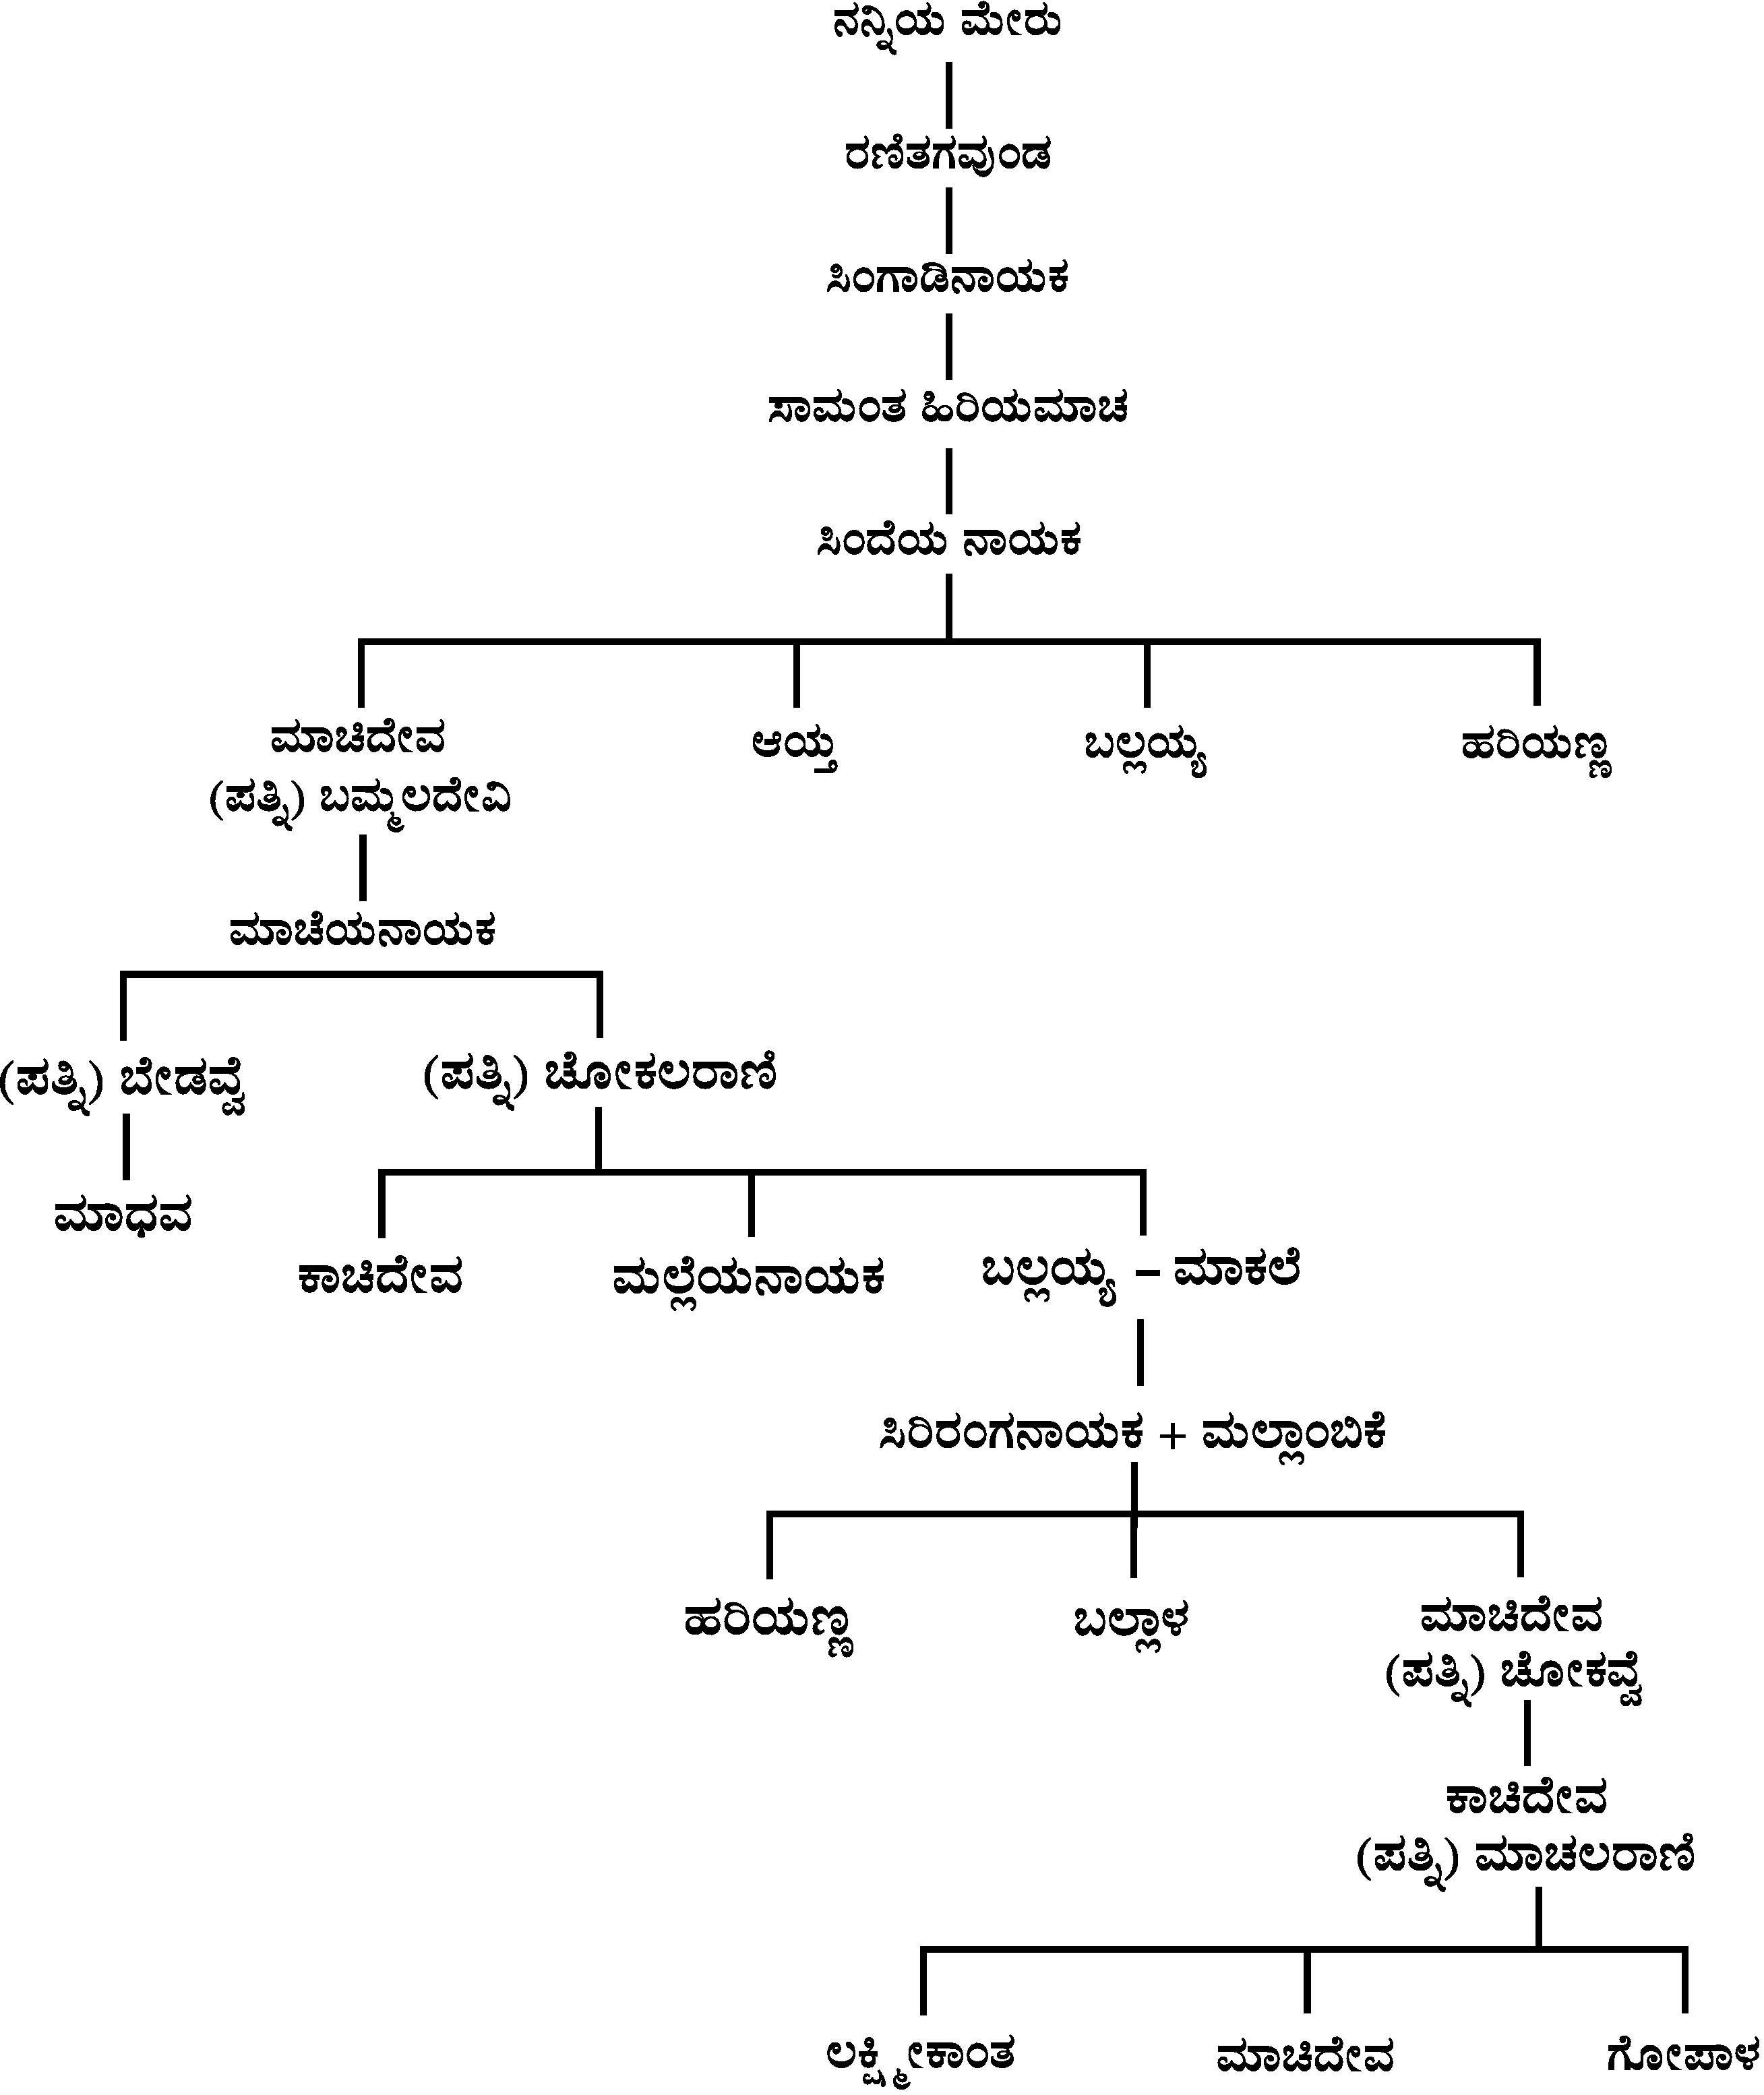
\includegraphics[scale=1.05]{images/chap3/chap3fig7.jpeg}
\end{figure}

ಎಪಿಗ್ರಾಫಿಯಾ ಕರ್ನಾಟಿಕಾ ಸಂಪಾದಕರು ಕಾಚೆಯ ನಾಯಕನ ವಂಶಾವಳಿಯನ್ನು ನೀಡಿದ್ದಾರೆ.\endnote{ ಎಪಿಗ್ರಾಫಿಯಾ ಕರ್ನಾಟಿಕಾ, ಸಂಪುಟ 7, ಪೀಠಿಕೆ, ಪುಟ \engfoot{lx}} ಈ ವಂಶಾವಳಿ\-ಯಲ್ಲಿ ಶಾಸನದಲ್ಲಿರುವ ಕೆಲವೊಂದು ಹೆಸರುಗಳು ಬಿಟ್ಟುಹೋಗಿವೆ. ಮಾಚೆಯನಾಯಕ ಮತ್ತು ಚೋಕಲ ರಾಣಿಯರ ಪುತ್ರ ಬಲ್ಲಯನ ಹೆಂಡತಿಯ ಹೆಸರನ್ನು ನೀಡಿರುವುದಿಲ್ಲ. ಆದರೆ ಶಾಸನದಲ್ಲಿ ಬಲ್ಲಯನ ಪತ್ನಿ ಮಾಕಲೆ ಎಂದಿದೆ. ಬಲ್ಲಯ್ಯ, ಮಾಕಲೆಯರ ಪುತ್ರ ಸಿರಿರಂಗನಾಯಕ. ಸಿರಿರಂಗನಾಯಕ ಮತ್ತು ಮಲ್ಲಾಂಬಿಕೆಯ ಪುತ್ರ ಮಾಚಿದೇವ. ಸಂಪಾದಕರು ಮಾಚಿದೇವನ ಪತ್ನಿಯ ಹೆಸರನ್ನು ನೀಡಿರುವುದಿಲ್ಲ. ಆದರೆ ಮಾಚಿದೇವನ ಪತ್ನಿಯನ್ನು “ಆ ಕೊಂತಿದೇವಿಗಧಿಕಂ ಚೋಕವ್ವೆ ನಾಯಕಿತ್ತಿ ಎಂದು ಹೇಳಿದೆ. ಇವರ ಮಗ ಕಾಚಿದೇವ. ಕಾಚಿದೇವನ ಪತ್ನಿಯ ಹೆಸರು ಶ‍್ರೀದೇವಿ ಎಂದು ಎಪಿಗ್ರಾಫಿಯಾ ಸಂಪಾದಕರು ಹೇಳಿದ್ದಾರೆ. ಆದರೆ ಶಾಸನದಲ್ಲಿ “ಕಾಚಿ ದೇವನ ಅರ್ಧಾಂಗ ಪುಣ್ಯ ಲಕ್ಷ್ಮಿ ಮಾಚಲೆನಾರಿ” ಎಂದು ಸ್ಪಷ್ಟವಾಗಿ ಶಾಸನದಲ್ಲಿ ಹೇಳಿದೆ, ಕಾಚಿ ದೇವನ ಪತ್ನಿ ಮಾಚಲೆ ನಾರಿ. ಇವರಿಗೆ ಲಕ್ಷ್ಮೀಕಾಂತ, ಮಾಚಿದೇವ, ಗೋಪಾಳ ಎಂಬ ಮೂವರು ಮಕ್ಕಳು ಎಂದು ಹೇಳಿದೆ. ಆದುದರಿಂದ ಎಪಿಗ್ರಾಫಿಯಾ ಸಂಪಾದಕರು ನೀಡಿರುವ ವಂಶಾವಳಿಯನ್ನು ಪರಿಷ್ಕರಿಸಿ ನೀಡಲಾಗಿದೆ.

ಬೆಳ್ಳೂರಿನ ಕ್ರಿ.ಶ.1199ರ ಶಾಸನೋಕ್ತ ಸಾಮಂತ ಸಿಂಧೆಯ ನಾಯಕನು\index{ಸಿಂಧೆಯ ನಾಯಕ}, ಮೇಲ್ಕಂಡ ಶಾಸನೋಕ್ತ ಸಾಮಂತ ಕಾಚಿ ದೇವನ ವಂಶಜನಿರಬಹುದೆಂದು ಎಪಿಗ್ರಾಫಿಯಾ ಸಂಪಾದಕರು ಊಹಿಸಿದ್ದಾರೆ.\endnote{ ಎಪಿಗ್ರಾಫಿಯಾ ಕರ್ನಾಟಿಕಾ, ಸಂಪುಟ 7, ಪೀಠಿಕೆ ಪುಟ \engfoot{lx,} ಎಕ 7 ನಾಮಂ 80 ಬೆಳ್ಳೂರು 1199} ಆದರೆ ಸಿಂಧೆಯ ನಾಯಕನ ವಂಶಜರಾದ ಬಾವಿಸೆಟ್ಟಿ, ಕೇತಿಸೆಟ್ಟಿ, ಮಂಡಲಸ್ವಾಮಿ ಇವರೆಲ್ಲರೂ ವ್ಯಾಪಾರಿಗಳಾಗಿದ್ದಾರೆ. ಕಾಚಿನಾಯಕ ವಂಶಜರು ಚತುರ್ಥ ಕುಲದವರು ಮತ್ತು ಮೊರಸಾದಿರಾಯರು, ಕುರುವಂದ ಕುಲದವರು ಎಂದು ಹೇಳಿದ್ದು ಒಬ್ಬರಿಗೊಬ್ಬರಿಗೆ ಸಂಬಂಧ\-ವಿಲ್ಲವೆಂದು ಹೇಳಬಹುದು.

\textbf{ಮಹಾಸಾಮಂತ ಜೋಗುಂಡಯ್ಯ\index{ಜೋಗುಂಡಯ್ಯ}(1247)}: ಮದ್ದೂರು ತಾಲ್ಲೂಕಿನ ಬೆಳತೂರಿನ ತ್ರುಟಿತ ತಮಿಳು ಶಾಸನದಲ್ಲಿ ವೀರಸೋಮೇಶ್ವರನ ಕಾಲದಲ್ಲಿ “ಮೇಲಿಪಿಳತ್ತೂರು ಶ‍್ರೀಮನ್ಮಹಾ ಸಾಮಂತನ ಮಗ ಕಾಲೈಯ ನಾಯಕನ ಮಗ \hbox{ಜೋಗುಣ್ಡಯ್ಯ”}\-ನಿಗೆ ದತ್ತಿ ಬಿಡಲಾಗಿದೆ.\endnote{ ಎಕ 7 ಮಂ 25 ಬೆಳತೂರು 1247-48} ಇವನು ತಮಿಳುನಾಡಿನ ಕಡೆಯಿಂದ ಬಂದ ಸೇನಾನಾಯಕ ಹಾಗೂ ಸಾಮಂತನಿರಬಹುದು. ಮಂಡ್ಯದ ಸಮೀಪ ಜೀಗುಂಡಿಪಟ್ಟಣ ಎಂಬ ಹಳ್ಳಿ ಇದ್ದು, ಇದರ ಮೂಲ ಹೆಸರು ಜೋಗುಂಡಯ್ಯ ಪಟ್ಟಣ\index{ಜೋಗುಂಡಯ್ಯ ಪಟ್ಟಣ} ಎಂದು ಊಹಿಸಬಹುದು. ಜೀಗುಂಡಿ ಪಟ್ಟಣದಲ್ಲೂ\index{ಜೀಗುಂಡಿ ಪಟ್ಟಣ} ಕ್ರಿ.ಶ.1320ರ ಒಂದು ತ್ರುಟಿತ ಶಾಸನ ಇದ್ದು, ಮಹಾನಾಯಕ ಒಡೆಯನ ಮತ್ತು ಗವುಡು ಪ್ರಜೆಗಳ ಪ್ರಸ್ತಾಪವಿದ್ದು ಈ ಊರನ್ನು ಪಟ್ಟಣವನ್ನಾಗಿ ಮಾಡಿದ ಸೂಚನೆಗಳಿವೆ.\endnote{ ಎಕ 7 ಮಂ 45 ಜೀಗುಂಡಿಪಟ್ಟಣ 1320}

\textbf{ಮಹಾಸಾಮಂತ ನಾಗಯ್ಯ\index{ನಾಗಯ್ಯ} (1280):} ಮುಮ್ಮಡಿ ಬಲ್ಲಾಳನ ಕಾಲದಲ್ಲಿ ಶ‍್ರೀಮನ್​ ಮಹಾಸಾಮಂತ ಹುಲಿಯಜಂಗುಳಿ ಮೊತ್ತದ ಸೇನಾನಾಯಕ ನಾಗಯ್ಯನೆಂಬುವವನು, ಕೆರೆಗೋಡಿನಾಡ ಹಾಡಿಮಂಡಲ ವೃತ್ತಿಯ ಎಮ್ಮೆಯಕೇತನಹಟ್ಟಿಯನ್ನು\index{ಎಮ್ಮೆಯ ಕೇತನಹಟ್ಟಿ} ಸಮಸ್ತ ಗಾವುಂಡುಗಳ ಸಮ್ಮುಖದಲ್ಲಿ, ಕಲಿದೇವರಿಗೆ ಶಿವಪುರವನ್ನಾಗಿ\index{ಶಿವಪುರ} ಮಾಡಿ \textbf{ಭಕ್ತರಿಗೆ }ದತ್ತಿ ಬಿಡುತ್ತಾನೆ.\endnote{ ಎಕ 7 ಮಂ 13 ಮರಡಿಪುರ 1280}


\section*{ಸಾಮಂತರು\index{ಸಾಮಂತರು}}

ಸಾಮಂತರೂ ಕೂಡಾ ಸೇನಾ ಪ್ರಮುಖರಾಗಿದ್ದು, ಮಹಾಸಾಮಂತರ ಅಧೀನರಾಗಿ ತಮ್ಮ ಶೌರ್ಯ ಪರಾಕ್ರಮದಿಂದ ಯುದ್ಧಕಾಲದಲ್ಲಿ ರಾಜನಿಗೆ ಸೇನೆಯ ನೆರವನ್ನು ನೀಡುತ್ತಾ, ತಾವೂ ಹೋರಾಡಿ, ತಮಗೆ ವಂಶಪಾರಂಪರ್ಯವಾಗಿ ಬಂದ ಪ್ರದೇಶಗಳನ್ನು ಆಳಿಕೊಂಡು, ಧಾರ್ಮಿಕ ಹಾಗೂ ಸಾಮಾಜಿಕ ಕೆಲಸಗಳನ್ನು ಮಾಡಿಕೊಂಡು ಬರುತ್ತಿದ್ದರೆಂಬುದು ಹೊಯ್ಸಳರ ಶಾಸನಗಳಿಂದ ತಿಳಿದುಬರುತ್ತದೆ. ಕೃಷ್ಣರಾಜಪೇಟೆ ತಾಲ್ಲೂಕಿನ, ತೆಂಗಿನಘಟ್ಟ ಶಾಸನದಲ್ಲಿ ಬೆಸಟೆಯ ಸಾವಂತ, ಕೋಟೆಯ ಸಾವಂತ ಎಂದು ಎರಡು ಬಗೆಯ ಸಾಮಂತರನ್ನು ಹೇಳಿದೆ.\endnote{ ಎಕ 6 ಕೃಪೇ 42 ತೆಂಗಿನಘಟ್ಟ 1117} ಬೆಸಟೆಯ ಸಾಮಂತನೆಂದರೆ ಆಜ್ಞಾಪಿಸುವ ಆಡಳಿತ ಅಧಿಕಾರವನ್ನು ಹೊಂದಿದ ಸಾಮಂತನೆಂದೂ, ಕೋಟೆಯ ಸಾಮಂತನೆಂದರೆ ಕೋಟೆಯನ್ನು ಕಾಯುತ್ತಾ ಊರಿನ ರಕ್ಷಣೆಯ ಭಾರ ಹೊತ್ತಿದ್ದ ಸಾಮಂತನೆಂದು ಹೇಳಬಹುದು..

\textbf{ಸಾಮಂತ ಸೋಮ\index{ಸಾಮಂತ ಸೋಮ} ಅಥವಾ ಸೋವೆಯನಾಯಕ (1142):} ವಿಷ್ಣುವರ್ಧನನ ಪಾದ ಪದ್ಮೋಪಜೀವಿಯಾಗಿ ಕಲುಕಣಿ ನಾಡನ್ನು\index{ಕಲುಕಣಿ (ಕಲಿಕಣಿ-ಕಲ್ಕಣಿ-ಕಲ್ಕುಣಿ-ಕಲುಕರೆ) ನಾಡು} ಆಳುತ್ತಿದ್ದ, ಸಾಮಂತ ಸೋಮ ಅಥವಾ ಸೋವೆಯ ನಾಯಕನ ವಂಶದ ಕುತೂಹಲಭರಿತ ಇತಿಹಾಸವನ್ನು ಕಸಲಗೆರೆಯ\index{ಕಸಲಗೆರೆ} ಶಾಸನವು ವಿವರವಾಗಿ ನೀಡುತ್ತದೆ.\endnote{ ಎಕ 7 ನಾಮಂ 169 ಕಸಲಗೆರೆ 1142} ಈ ಶಾಸನವು \textbf{“ಸ್ವಸ್ತಿ ಸ್ವಸ್ತಿಳಕೈಃ ಶುಭೈಃ ಶುಭಾವತೈಃ ಪುಣ್ಯಾಹವೈಃ ಕೀರ್ತ್ರಯಾಂ ಸ್ಥಾಪ್ಯಂತೇ ಜಿತಪಾರ್ಶ್ವಂ ಜಿನಪಾದಪಂಕಜ ದಳೇ ಶ‍್ರೀಹ್ರೀಧೃತಿದ್ಧಾರ್ಯತಾಂ ತ್ವಂ ದತ್ತಂ ದೇಯಾತು ದೇವ ದೇವಭುವನೇ ಮುಕ್ತ್ಯಾಂಗನವಲ್ಲಭೋ ಸಾಮಂತಂ ಜಯಜೀಯವರ್ದ್ಧನಕರಂ ಸೋಮಂ ಸ್ಥಿರಂ ಜೀಯಾತು”} ಎಂದು ಸಾಮಂತ ಸೋಮನ ಸ್ತುತಿಯೊಂದಿಗೆ ಪ್ರಾರಂಭವಾಗಿರುವುದು ಒಂದು ವಿಶೇಷ. ಚೋಳ ಬಲವನ್ನು ಅಲ್ಲೋಲಕಲ್ಲೋಲ ಮಾಡುವಂತಹ ಹಿರಿದಾದ ದಂಡನ್ನು ತೆಗೆದುಕೊಂಡು ಬಂದ ವೀರಪೆರ್ಮಾಡಿ ದೇವನು\index{ವೀರಪೆರ್ಮಾಡಿ ದೇವ} ಹೃದುವನ ಕೆರೆಯಲ್ಲಿ\index{ಹೃದುವನ ಕೆರೆ} ಬೀಡುಬಿಟ್ಟನು. ಈ ಸೇನೆಯ ಬೀಡಿನ ಮೇಲೆ ಮದಿಸಿದ ಆನೆಯು ನುಗ್ಗಿತು. ಚೋಳನ ಮೇಲೆ ನಡೆಯುತ್ತ ಬಂದ ಸೇನೆಯ ಮೇಲೆ ಕಾಡಾನೆಯು ಕವಿಯಲು, ಆ ಊರಿನ ಅಯ್ಯಣ ಅಥವಾ ಅಯ್ಕಣನು ಬಾಣದಿಂದ ಆನೆಯ ಕುಂಭಸ್ಥಳವನ್ನು ಭೇದಿಸಿ ಅದನ್ನು ಕೊಂದನು. ಆಗ ಬಹುಶಃ ಗಂಗರಾಜನ (ವೀರ ಪೆರ್ಮಾಡಿ) ಆದೇಶದ ಮೇರೆಗೆ, ಅಯ್ಕಣನನ್ನು, ಕಲುಕಣಿ ನಾಡಾಳ್ವನು ಕರಿಯಅಯ್ಕಣನೆಂದು\index{ಕರಿಯಅಯ್ಕಣ} ಕರೆದು ವೀರಪಟ್ಟವನ್ನು ಕಟ್ಟಿದನು. \textbf{“ಅಯ್ಕಣನಿಗೆ ಕರಿಯ ಅಯ್ಕಣನೆಂಬ ಪಟ್ಟವೂ ಕಲುಕಣಿ ನಾಡಿನ ಒಡೆತನವೂ ದೊರೆಯಿತೆಂದು” ಎಪಿಗ್ರಾಫಿಯಾ ಕರ್ನಾಟಿಕಾ ಸಂಪಾದಕರು ಹೇಳಿದ್ದಾರೆ.\endnote{ ಎಪಿಗ್ರಾಫಿಯಾ ಕರ್ನಾಟಿಕಾ, ಸಂಪುಟ 7, ಪೀಠಿಕೆ, ಪುಟ liv} ಆದರೆ ಶಾಸನದಲ್ಲಿ “ಅಯ್ಕಣಂ ಕರಿಯನೆಚ್ಚಡೆ ಕಲುಕಣಿ ನಾಡಾಳ್ವಂ, ಕರಿಯಯ್ಕಣನೆಂದು ವೀರಪಟ್ಟಮಂ ಕಟ್ಟಿ” ಎಂದು ಸ್ಷಷ್ಟವಾಗಿ ಹೇಳಿದೆ. ಅಯ್ಕಣನಿಗೆ ದೊರಕಿದ್ದು ವೀರಪಟ್ಟ ಮಾತ್ರ. ಕಲುಕಣಿ ನಾಡಾಳ್ವನು ಅಂದರೆ ನಾಡನ್ನು ಆಳುತ್ತಿದ್ದವನು ಇವನಿಗೆ ವೀರಪಟ್ಟವನ್ನು ಕಟ್ಟಿದನೆಂದು ಹೇಳಿದೆ.} ಕರಿ ಅಯ್ಕಣನ ಮಗ ನಾಗ\index{ನಾಗ}. ಈ ನಾಗನಿಂದ ನಾಗಮಂಗಲ\index{ನಾಗಮಂಗಲ} ಎಂಬ ಹೆಸರು ಬಂದಿರಬಹುದು. ನಾಗನ ಹಿರಿಯ ಮಗ ಅದಿರದ ಗಂಡನೆನಿಸಿದ ಸುಗ್ಗಗೌಂಡ. ಇವನ ಮಗ ಸೋಮ. ಇವನಿಗೆ ಸಾಮಂತ ಪಟ್ಟ ದೊರೆತು ಸಾಮಂತ ಸೋಮನೆನಿಸಿದನು\index{ಸಾಮಂತ ಸೋಮ}. ಸೋಮನ ಹೆಂಡತಿ ಮಾರವ್ವೆ(ಯ್ವೆ). ಇವರಿಗೆ ಚಟ್ಟದೇವ, ಕಲಿದೇವ, ಮತ್ತು ಸೋವಣ ಎಂಬ ಮೂರು ಜನ ಮಕ್ಕಳು. ಶಾಸನವು ಸೋಮನನ್ನು ಅತಿಶಯವಾಗಿ ವರ್ಣಿಸಿದೆ. \textbf{‘ಪನ್ನಗವೈನತೇಯ’}ನೆನಿಸಿದ್ದ ಸೋಮನು ಅನೇಕ ಯುದ್ಧಗಳಲ್ಲಿ ಶತ್ರುಗಳನ್ನು ತರಿದಿಕ್ಕಿದನು. \textbf{“ಸ್ವಸ್ತಿ ಸಮಸ್ತ ಗುಣ ಸಂಪನ್ನನುಂ ವಿಬುಧಪ್ರಸನ್ನನುಂ ಆಹಾರಾಭಯಭೈಷಜ್ಯ ಶಾಸ್ತ್ರ ವಿನೋದನುಂ ಜಿನಗನ್ಧೋದಕ ಪವಿತ್ರೀಕೃತೋತ್ತಮಾಂಗನುಂ ಜಿನಸಮಯ ಸಮುದ್ಧರಣನುಂ ತೊಡರ್ದರಡೊಂಕಿಯುಂ ತೊಡರೆಬಲ್ಗಂಡನುಂ ನುಡಿದುಮತ್ತೆನ್ನನುಂಪರನಾರೀಪುತ್ರನುಂ ಪಾರ್ಶ್ವದೇವ ಪಾದಾರಾಧಕನುಮಪ್ಪಕಲುಕಣಿ ನಾಡಾಳ್ವ ಸಾವಂತ ಸೋವೆಯನಾಯಕಂ ಭಾನುಕೀರ್ತ್ತಿ ಸಿದ್ಧಾನ್ತದೇವರ ಗುಡ್ಡಂ”} ಎನಿಸಿದ ಸಾಮಂತ ಸೋಮೆಯ ನಾಯಕನು, ಹೆಬ್ಬಿದಿರೂರ್ವಾಡಿಯಲ್ಲಿ\index{ಹೆಬ್ಬಿದಿರ (ಹೆಬ್ಬಿದರ) ವಾಡಿ, ಹೆಬ್ಬಿದಿರೂರ್ವಾಡಿ (ಕಸಲಗೆರೆ)} (ಇದೇ ಕಸಲಗೆರೆಯ\index{ಕಸಲಗೆರೆ} ಪ್ರಾಚೀನ\break ಹೆಸರು) ಉತ್ತುಂಗ ಚೈತ್ಯಾಲಯವನ್ನು ಮಾಡಿಸಿ, ಶ‍್ರೀ ಪಾರ್ಶ್ವದೇವರ ಪ್ರತಿಷ್ಠೆಯನ್ನು ಮಾಡಿ, ಶ‍್ರೀ ಮೂಲಸಂಘದ\break ಸೂರಸ್ತ ಗಣದ ಬ್ರಹ್ಮದೇವರಿಗೆ ದತ್ತಿಯನ್ನು ಬಿಡುತ್ತಾನೆ. ಸಾಮಂತ ಸೋಮನ ವಂಶಾವಳಿಯಲ್ಲಿ ಇದು ಮೊದಲನೆಯ ಹಂತ. ಇದೇ ಕಸಲಗೆರೆಯ ಇನ್ನೊಂದು ತ್ರುಟಿತ ಶಾಸನವು ಬಹುಶಃ ಸಾಮಂತ ಸೋಮನ ಮಗ ಸೋವಣ\index{ಸೋವಣ} ಅಥವಾ ಸೋಮನನ್ನು \textbf{“ಕೂಡಲೂರ ಕುಲಕಮಲ ಮಾರ್ತಾಂಡ\index{ಕೂಡಲೂರ ಕುಲಕಮಲ ಮಾರ್ತಾಂಡ}”}ನೆಂದು ವರ್ಣಿಸಿದೆ. ಈತನ ಪುತ್ರ ಅನುಪಮದಾನಿ ಗಂಡುಗಲಿ ಮಾರದೇವನು\index{ಮಾರದೇವ} ಯಾವುದೋ ಯುದ್ಧದಲ್ಲಿ ಮಡಿಯಲು ಅವನ ಸತಿ \textbf{“ಮಹಾದೇವಿ\index{ಮಹಾದೇವಿ} ತನ್ನ ವರನೊಳು ಪ್ರತಿಪನ್ನದಿ ಸಂದಳಾದಿವಂ” }ಎಂದು ತಿಳಿದುಬರುತ್ತದೆ.\endnote{ ಎಕ 7 ನಾಮಂ 171 ಕಸಲಗೆರೆ 12ನೇ ಶ.} ಸಾಮಂತಸೋಮನ ಕಾಲ 1142. ಅವನ ಮಗ ಸಾವಂತ ಸೋಮನು ಒಂದನೆಯ ನರಸಿಂಹ ಅಥವಾ ವೀರ ಬಲ್ಲಾಳನ ಕಾಲದವನಿರಬಹುದು. ವೀರ ಬಲ್ಲಾಳನ ಕಾಲದಲ್ಲಿ ಶೈವಧರ್ಮವು ಪ್ರಬಲಿಸಿ ಜೈನಬಸದಿಗಳಿಗೆ ಧಕ್ಕೆಯಾದ ಕಾರಣ, ಸಾಮಂತ ಸೋಮನು ಕಟ್ಟಿಸಿದ ಚೈತ್ಯಾಲಯವನ್ನು ಎಕ್ಕೋಟಿ ಜಿನಾಲಯವೆಂದು\index{ಎಕ್ಕೋಟಿ ಜಿನಾಲಯ} ಘೋಷಿಸಲಾಯಿತು.\endnote{ ಎಕ 7 ನಾಮಂ 170 ಕಸಲಗೆರೆ 12ನೇ ಶ.}

ಸಾಮಂತ ಸೋಮೆಯನ ಮಗ ಮಲ್ಲೆ ಸಾಮಂತನು\index{ಮಲ್ಲೆ ಸಾಮಂತ} ತೊಂಡನೂರ ಬಲ್ಲಾಳದಾಸರ\index{ತೊಂಡನೂರ ಬಲ್ಲಾಳದಾಸ} ದೇವರಿಗೆ, ಸಿರಕುಬಳ್ಳಿ, ಭೋಗನಹಳ್ಳಿ, ಚೆಟ್ಟಹಳ್ಳಿ, ಬಾಗಸೆಟ್ಟಿಹಳ್ಳಿಗಳನ್ನು ದತ್ತಿಯಾಗಿ ನೀಡಿದ್ದಾನೆ.\endnote{ ಎಕ 6 ಪಾಂಪು 77 ತೊಣ್ಣೂರು 13ನೇ ಶ.} ಇವನು ಮಾರ ದೇವನ ತಮ್ಮನಿರಬಹುದು. ಈ ಶಾಸನವು ವೀರಬಲ್ಲಾಳನ ಕಾಲದ್ದಿರಬಹುದೆಂದು ಊಹಿಸಬಹುದು. ಸಾಮಂತ ಮಾರ ನಾಯಕನ ಮಗನಾದ ಮಾಚಿದೇವ ಅಥವಾ ಮಾಚನು ಕಲುಕಣಿ ನಾಡಿನ ಸಾಮಂತನಾಗಿ ಮುಂದುವರಿದನು. ಮೂರನೆಯ ನರಸಿಂಹನು ಮಲೆಯ ದಂಡಿಗೆತ್ತಿ ನಡೆವಲ್ಲಿ, ಈ ಸಾಮಂತ ಮಾಚನ ಮಗ ಗುಜ್ಜೆಯ ನಾಯಕನು\index{ಗುಜ್ಜೆಯ ನಾಯಕ} ಹೋರಾಡಿ ಮಡಿದನೆಂದು, ಅಲ್ಲೇ ಇರುವ ಮತ್ತೊಂದು ಶಾಸನ ಹೇಳುತ್ತದೆ.\endnote{ ಎಕ 7 ನಾಮಂ 172 ಕಸಲಗೆರೆ 1260} ಸಾಮಂತ ಮಾಚೀದೇವ ಅವನ ಸತಿ ಕೇತಲದೇವಿ ಮತ್ತು ಇವರ ಮಗ ಗುಜ್ಜೆಯ ನಾಯಕ ಇವರುಗಳನ್ನು ಶಾಸನ ವರ್ಣಿಸಿದೆ.

\textbf{“ಮಾಚಿದೇವನ ಕುಲದೀಪನುಮೆನಿಪ ಗುಜ್ಜಯನಾಯ್ಕನ ವರಕೀರ್ತ್ತಿಯಂ ದಿವಿಜಲಲನೆಯರು ಕೇಳ್ದಿದಿರುವಂದು\general{\break } ಸ್ವರ್ಗಲೋಕಸುಕಪ್ರಾಪ್ತನೆಂದು ಸ್ವರ್ಗ್ಗಕ್ಕೆ ಒಯ್ದರು”} ಎಂದು ಅವನ ವೀರತ್ವವನ್ನು ಬಣ್ಣಿಸಲಾಗಿದೆ. ಎಪಿಗ್ರಾಫಿಯಾ ಸಂಪಾದಕರು ಸಾಮಂತ ಸೋಮನವರೆಗೆ ವಂಶಾವಳಿಯನ್ನು ನೀಡಿದ್ದಾರೆ.\endnote{ ಎಪಿಗ್ರಾಫಿಯಾ ಕರ್ನಾಟಿಕಾ, ಸಂಪುಟ 7, ಪೀಠಿಕೆ ಪುಟ \engfoot{liv} (ಸಾವಂತ ಸೋಮನವರೆಗೆ ವಂಶಾವಳಿಯನ್ನು ನೀಡಿದೆ)} ಡಾ. ವೈ.ಸಿ. ಭಾನುಮತಿಯವರು ಕೂಡಾ ಒಂದು ವಂಶಾವಳಿಯನ್ನು ನೀಡಿದ್ದಾರೆ.\endnote{ ಭಾನುಮತಿ, ಡಾ॥ ವೈ.ಸಿ., ಮಂಡ್ಯ ಜಿಲ್ಲೆಯ ಸ್ಥಾನಿಕ ಪ್ರಭುಗಳು, ಸಮಾಗತ, ಪುಟ 60} ಆದರೆ ಮೇಲಿನ ಶಾಸನಗಳಿಂದ ಸಾಮಂತ ಸೋಮೆಯ ನಾಯಕನ ವಂಶವನ್ನು ಈ ಕೆಳಗಿನಂತೆ ಪೂರ್ಣವಾಗಿ ಕಟ್ಟಿಕೊಡಬಹುದು.

\begin{figure}[H]
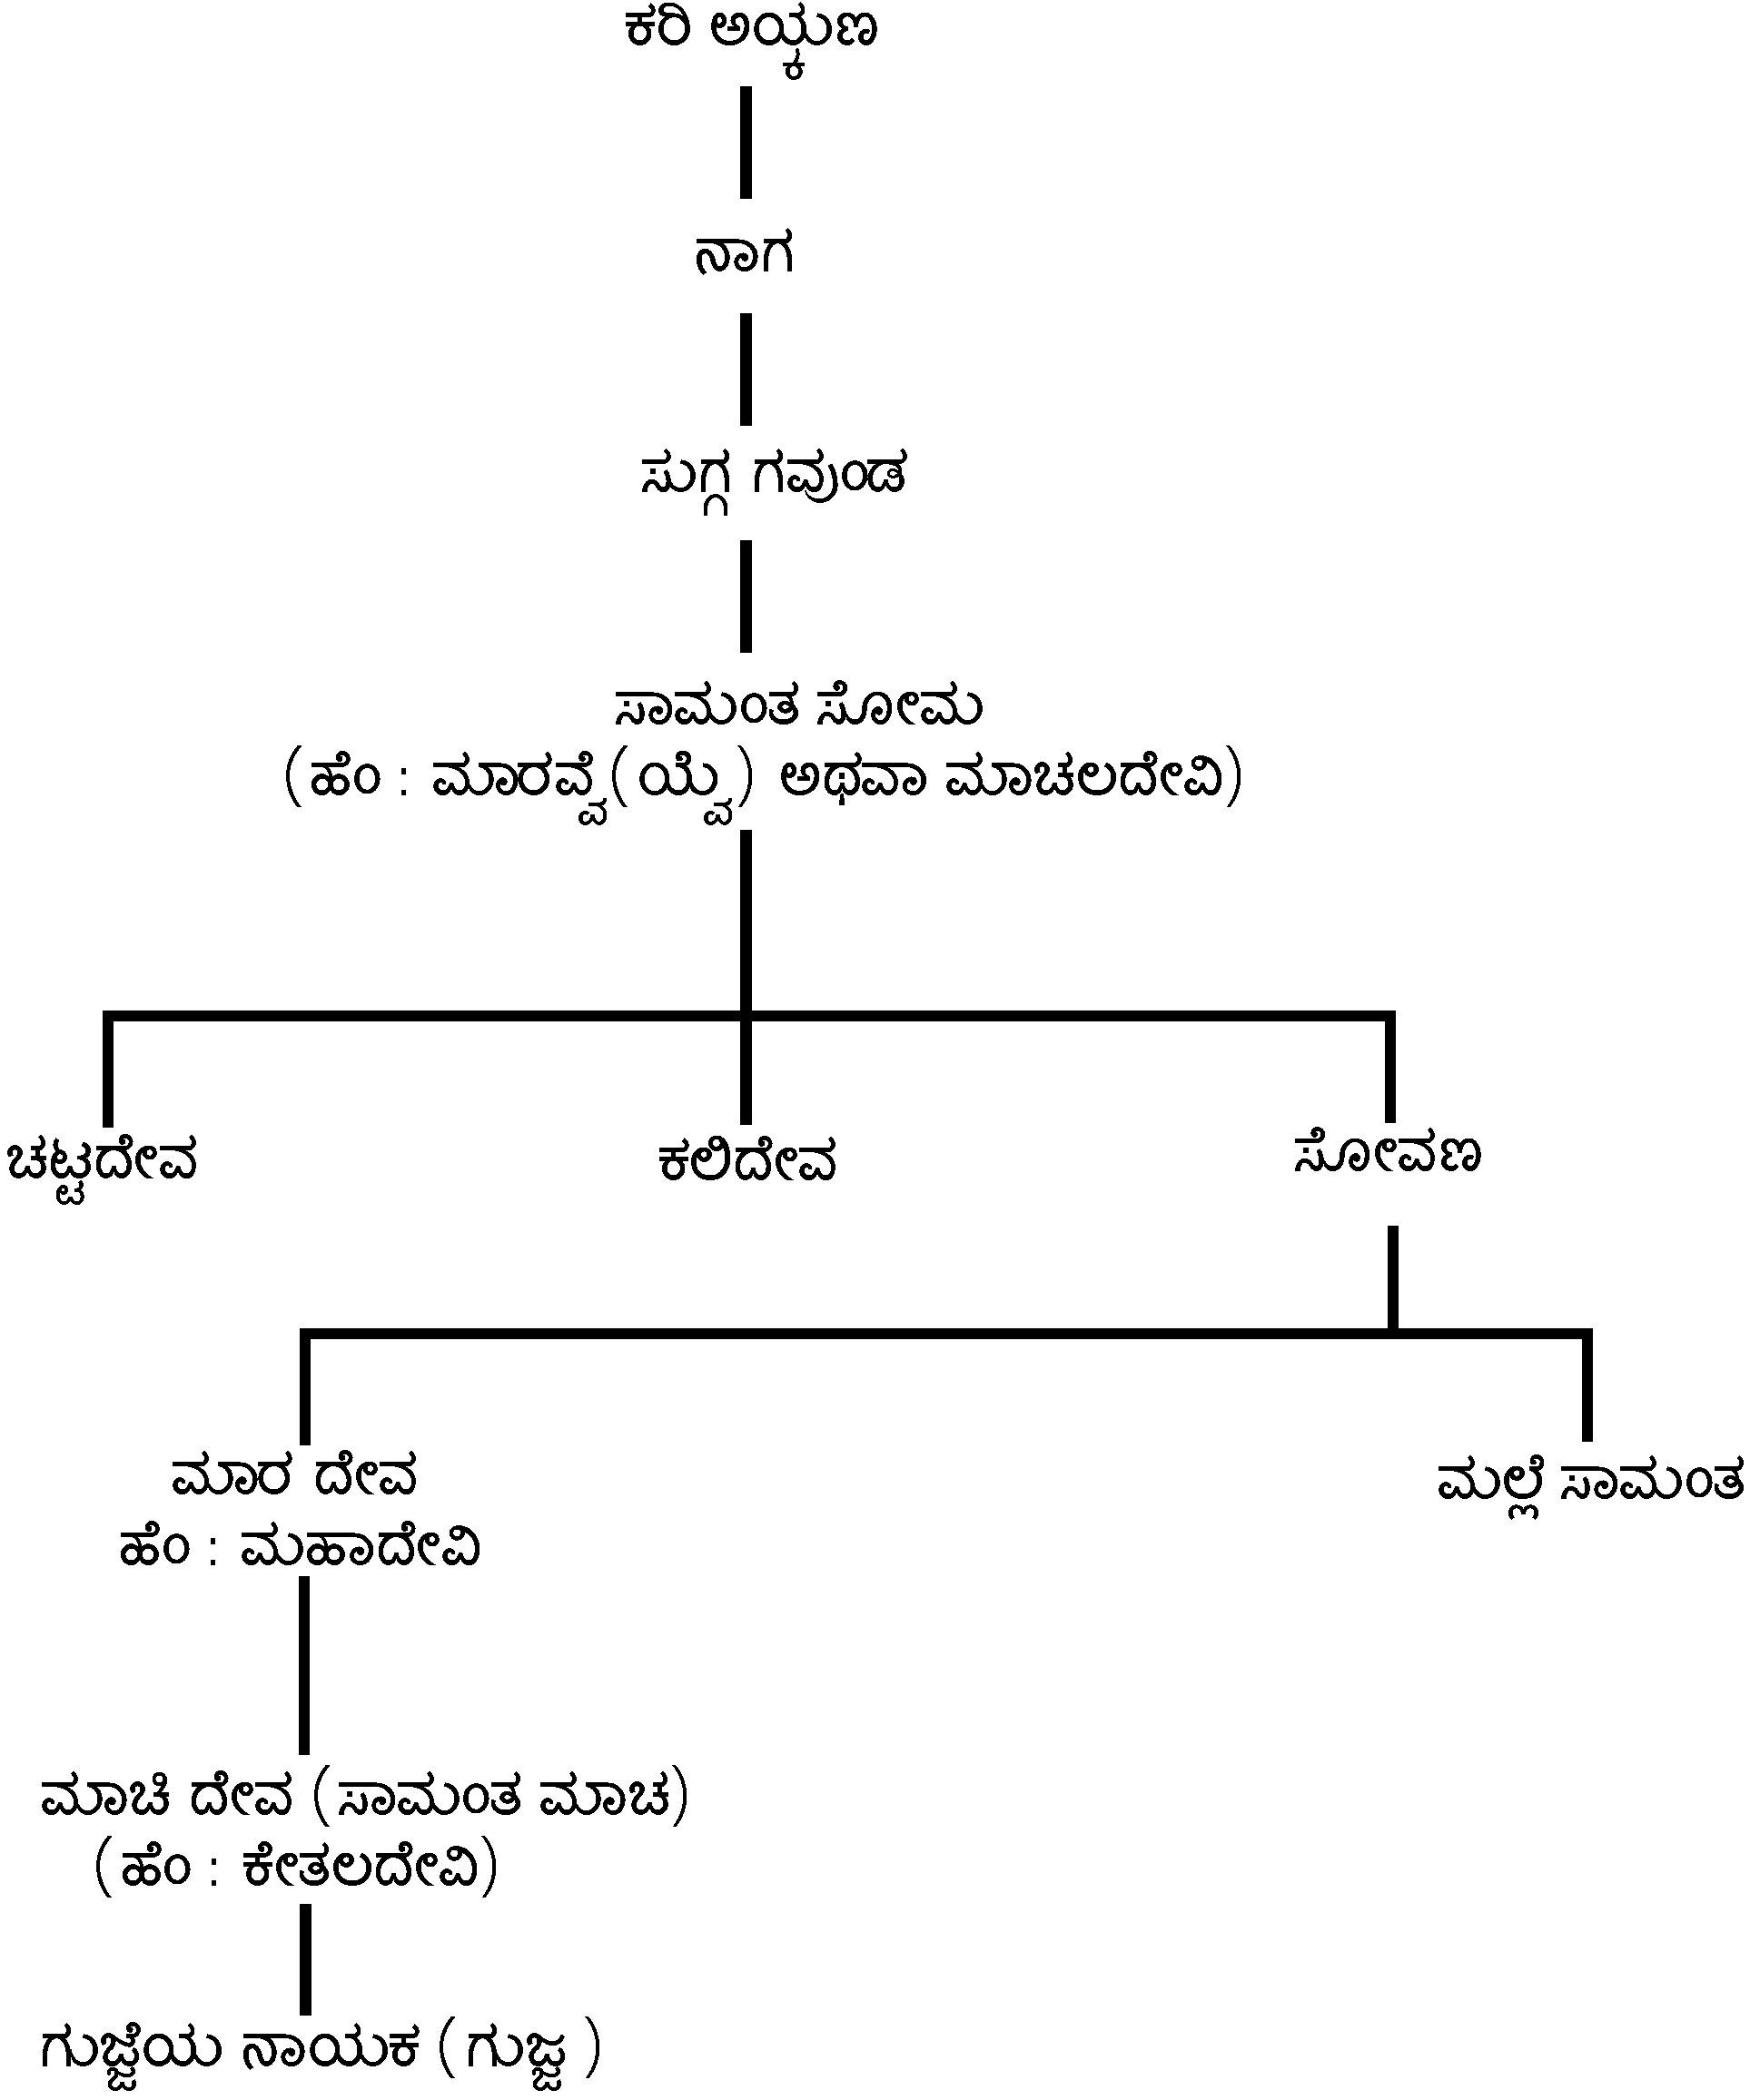
\includegraphics[scale=1.3]{images/chap3/chap3fig8.jpeg}
\end{figure}

ಕರಿ ಅಯ್ಕಣನು\index{ಕರಿ ಅಯ್ಕಣನು} ಚೋಳರ ವಿರುದ್ಧ ದಂಡೆತ್ತಿ ಹೋದ ವೀರಗಂಗ ಪೆರ್ಮಾನಡಿಯ ಕಾಲದವನೆಂದು ಹೇಳಿದೆ. ಈ ವೀರಗಂಗ ಪೆರ್ಮಾನಡಿ ಯಾರೆಂಬುದು ತಿಳಿಯದು ಎಂದು ಎಪಿಗ್ರಾಫಿಯಾ ಕರ್ನಾಟಿಕಾ ಸಂಪಾದಕರು ಹೇಳಿದ್ದಾರೆ.\endnote{ ಎಕ ಸಂಪುಟ 7 ಪೀಠಿಕೆ, ಪುಟ liv} ಸಾಮಂತ ಸೋಮನ ಕಾಲ ಕ್ರಿ.ಶ.1142. ಕರಿ ಅಯ್ಕಣನು ಇಲ್ಲಿಂದ ನಾಲ್ಕು ತಲೆಮಾರು ಹಿಂದಿನವನು. ಒಂದು ತಲೆಮಾರಿಗೆ 25 ವರ್ಷವೆಂದು ಇಟ್ಟುಕೊಂಡರೂ ನಾಲ್ಕು ತಲೆಮಾರಿಗೆ 100 ವರ್ಷ ಆಗುತ್ತದ. ಅಲ್ಲಿಗೆ ಈತನ ಕಾಲ ಸುಮಾರು 942 ಎಂದು ಊಹಿಸಬಹುದು. ಆಗ ಇಮ್ಮಡಿ ಬೂತುಗನು\index{ಇಮ್ಮಡಿ ಬೂತುಗ} ರಾಜ್ಯವಾಳುತ್ತಿದ್ದನು. ಚೋಳರ ವಿರುದ್ಧ ರಾಷ್ಟ್ರಕೂಟರ ಮೂರನೆಯ ಕೃಷ್ಣನ ಜೊತೆ ತಕ್ಕೋಲಂನಲ್ಲಿ ಹೋರಾಡಿ ಅವರನ್ನು ಸೋಲಿಸಿದ್ದಲ್ಲದೆ, ರಾಷ್ಟ್ರಕೂಟರ ಸೇನೆಯ ಜೊತೆ ಚೋಳ ರಾಜ್ಯದಲ್ಲಿ ನುಗ್ಗಿ ತಂಜಾವೂರನ್ನು ಗೆಲ್ಲಲು ನೆರವಾದನು.\endnote{ ಸೂರ್ಯನಾಥ ಕಾಮತ್​ ಡಾ॥, ಕರ್ನಾಟಕದ ಸಂಕ್ಷಿಪ್ತ ಇತಿಹಾಸ, ಪುಟ 35} ಚೋಳ ಬಲವನ್ನು ಅಲ್ಲೋಲಕಲ್ಲೋಲ ಮಾಡುವ ದಂಡನ್ನು ವೀರಗಂಗ ಪೆರ್ಮಾನಡಿಯು ತೆಗೆದುಕೊಂಡು ಬರುತ್ತಿದ್ದನೆಂಬುದು ಇದಕ್ಕೆ ಪುಷ್ಟಿಯನ್ನು ನೀಡುತ್ತದೆ. ಆದುದರಿಂದ ಈ ಶಾಸನೋಕ್ತ ವೀರಗಂಗ ಪೆರ್ಮಾನಡಿಯು ಇಮ್ಮಡಿ ಬೂತುಗನೇ ಆಗಿದ್ದಾನೆಂದು ಹೇಳಬಹುದು. ಕರಿ ಅಯ್ಕಣನ ಮಗ ನಾಗನ ಹೆಸರು ಕಂಬದಹಳ್ಳಿಯ ಕ್ರಿ.ಶ.10ನೇ ಶತಮಾನದ ಲಿಪಿಯಲ್ಲಿರುವ ಮಾನಸ್ಥಂಬ ಶಾಸನದಲ್ಲಿ ಬಂದಿದೆ.\endnote{ ಎಕ 7 ನಾಮಂ 33 ಕಂಬದಹಳ್ಳಿ, ಸೀತಾರಾಮಜಾಗಿರ್​ದಾರ್​, ಕಂಬದಹಳ್ಳಿ: ಒಂದು ಜೈನಕೇಂದ್ರ, ಪುಟ 9}\textbf{“ಪಲ್ಲಪಂಡಿತ ನಾಗೇಣ ದದತಾ ದಾನಮದ್ಭುತಂ ಭೂಷಿತಂ ಕಲಿಕಾಳೇಸ್ಮಿನ್ಗಂಗಮಂಡಲ ಕಾನನಂ”.} ಈ ಪ್ರದೇಶವು ಗಂಗಮಂಡಲ ಕಾನನ\index{ಗಂಗಮಂಡಲ ಕಾನನ} ಎಂದು ಹೆಸರಾಗಿತ್ತು. ನಾಗನು ಇದನ್ನು ಪಲ್ಲಪಂಡಿತರಿಗೆ\index{ಪಲ್ಲ ಪಂಡಿತ} ದಾನ ನೀಡಿದನು. ನಾಗನು ಬ್ರಾಹ್ಮಣರಿಗೆ ಅಗ್ರಹಾರವಾಗಿ ಬಿಟ್ಟ ಊರೇ ನಾಗಮಂಗಲ\index{ನಾಗಮಂಗಲ}. ನಾಗಮಂಗಲವು ಕಸಲಗೆರೆಗೆ ಸಮೀಪದಲ್ಲಿಯೇ ಇದೆ. ಹಾಗೂ ಈ ಶಾಸನದಲ್ಲಿ ನಾಗಮಂಗಲಕ್ಕೆ ಹೋಗುವ ದಾರಿ ಎಂದೂ ಕೂಡಾ ಉಲ್ಲೇಖವಾಗಿದೆ. ಕಂಬದಹಳ್ಳಿ ಶಾಸನೋಕ್ತ ನಾಗನು ಕಸಲಗೆರೆ ಶಾಸನೋಕ್ತ ಕರಿ ಅಯ್ಕಣನ ಮಗನೇ ಆಗಿದ್ದಾನೆಂದು ಹೇಳಬಹುದು. ಬೇಲೂರು ತಾಲ್ಲೂಕಿನ ತುಂಬದೇವನಹಳ್ಳಿಯ ಕ್ರಿ.ಶ.1096ರ ಶಾಸನದಲ್ಲಿ ಕದಂಬ ವಂಶದ ಕಲಿ ಹೃದುವ ನೃಪನ ಹೆಸರಿದೆ.\endnote{ ಎಕ 9 ಬೇಲೂರು 513 ತುಂಬದೇವನಹಳ್ಳಿ 1096} ಹೃದುವನಕೆರೆಗೂ ಇವನಿಗೂ ಏನಾದರೂ ಸಂಬಂಧ ಇದೆಯೇ ತಿಳಿಯದು. ಕಸಲಗೆರೆಯ ಸಮೀಪದಲ್ಲಿ ಇರುವ ಹಿದುವ\index{ಹಿದುವ} (ಹಿಡುವ) ಎಂಬ ಹಳ್ಳಿಯೇ ಹೃದುವನ ಕೆರೆ ಎಂದು ಊಹಿಸಬಹುದು.

\textbf{ಸಾಮಂತ ಕಾಳೆಯನಾಯಕ\index{ಕಾಳೆಯನಾಯಕ} (ಸು.1150):} ವಿಷ್ಣುವರ್ಧನನ ಕಾಲದಲ್ಲಿದ್ದ ಹಡವಳದ ಕೊಳ್ಳಿ ಅಯ್ಯ\index{ಹಡವಳದ ಕೊಳ್ಳಿ ಅಯ್ಯ} ಮತ್ತು ಚಾವುಂಡವ್ವೆ\-ಯರ\index{ಚಾವುಂಡವ್ವೆ} ಪುತ್ರರಲ್ಲಿ ಒಬ್ಬನಾದ ಕಾಳೆಯ ನಾಯಕನು,\endnote{ ಎಕ 6 ಕೃಪೇ 42 ತೆಂಗಿನಘಟ್ಟ 1117} ಒಂದನೇ ನರಸಿಂಹನ ಆಳ್ವಿಕೆಯ ವೇಳೆಗೆ ಸಾಮಂತ ಪಟ್ಟವನ್ನು ಅಲಂಕರಿಸಿದ್ದನು.\endnote{ ಎಕ 6 ಕೃಪೇ 43 ತೆಂಗಿನಘಟ್ಟ 12ನೇ ಶ.}\textbf{“ಸ್ವಸ್ತಿ ಶ‍್ರೀಮತು ತೆಂಗಿನಕಟ್ಟದ ಹಿರಿಯಹಡವಳ ಕೊಳ್ಳಿಯಮ್ಮೆಯಂಗಳ ಸುಪುತ್ರನಪ್ಪ ಸ್ವಸ್ತಿ ಸಮಸ್ತ ಪ್ರಶಸ್ತಿ ಸಹಿತ ಸ್ವಾಮಿಯಂಗಸನ್ನಾಹ ಸಂಗ್ರಾಮ ಸಹಸ್ರಬಾಹು ಕದನತ್ರಿಣೇತ್ರನುಂ ಕರೆದೀವದಾನಿವುಂ ಸುಭಟರಾದಿತ್ಯನುಂ ಕಲಿಯುಗಮಾರ್ತಂಡನುಂ ಎಸ್ವುರಾದಿತ್ಯನುಂ ಸಯಿಗೋಲಪಾರ್ತನುಂ ಕಂಣ್ನಂಬಿನಾತನುಂ ಪರನಾರೀದೂರನುಂ ರಣರಂಗಧೀರನುಂ ಸುಭಟರಾದಿತ್ಯನುಂ ಸತ್ಯರಾಧೇಯನುಂ ಸ್ವಾಮಿದ್ರೋಹರಗಂಣ್ಡನುಂ ಸಾವನ್ತ ಕಾಳಯ್ಯಂ”} ಎಂದು ತೆಂಗಿನ ಘಟ್ಟ ಶಾಸನವು ಇವನನ್ನು ವರ್ಣಿಸಿದೆ. ಇವನನ್ನು ನರಸಿಂಹನು ಕರೆದು ಯಾವುದೋ ಹೋರಾಟಕ್ಕೆ ಬೆಸಸಲು, \textbf{‘ಆ ಬೆಸನಂ ಕೈಗೊಂಡು’} ಹೋರಾಡಿ ಮಡಿದಿರಬಹುದೆಂದು ಊಹಿಸಬಹುದು. ಒಂದನೆಯ ನಾರಸಿಂಹನು ಪಟ್ಟಕ್ಕೆ ಬಂದ ನಂತರ ಅವನ ವಿರುದ್ಧ ತಿರುಗಿಬಿದ್ದ ಕೊಂಗಾಳ್ವರು\index{ಕೊಂಗಾಳ್ವರು}/ಚೆಂಗಾಳ್ವರ\index{ಚೆಂಗಾಳ್ವರು} ಮೇಲೆ ಇವನು ಹೋರಾಡಿ ಮಡಿದಿರಬಹುದು. ನಾಗಮಂಗಲ ತಾಲ್ಲೂಕು ಹೊನ್ನೇನಹಳ್ಳಿ ಶಾಸನೋಕ್ತ ಸಾಮಂತ ಕಾಳೆಯ ನಾಯಕ ಮತ್ತು ದೇಕೆಯ ನಾಯಕರು ಇವರಿಂದ ಭಿನ್ನರೆಂದು ಹೇಳಬಹುದು.

\textbf{ಸಾಮಂತ\index{ಸಾಮಂತ} ಭರತೆಯ ನಾಯಕ\index{ಭರತೆಯ ನಾಯಕ}(1174):} ಚಂಗಿಕುಳ\index{ಚಂಗಿಕುಲ} ಕಮಲನಾದ ಸಾಮಂತ ಭರತೆಯ ನಾಯಕನು ಹೊಯ್ಸಳ ಸಣ್ನೆನಾಡನ್ನು\index{ಹೊಯ್ಸಳ ಸಣ್ನೆನಾಡು} ಆಳುತ್ತಿದ್ದನೆಂದು ತಿಳಿದುಬರುತ್ತದೆ. \textbf{“ಶ‍್ರೀಮನ್ಮಹಾವೀರರಾಜೇಂದ್ರ ಹೊಯ್ಸಳಸಣ್ನೆನಾಡಾಳ್ವ ಚಂಗಿಕುಳಕಮಳಮಾರ್ತಂಡನತುಳ ಭುಜಬಳಾವಷ್ಟಂಭ ಕಾಮಕೋಟಿದೇವಿ ವರಪ್ರಸಾದ ನಾಮಾವಳಿ ಮುಖ್ಯರಪ್ಪ ಸಾವನ್ತ ಭರತೆಯನಾಯಕಂ”} ಎಂದು ಶಾಸನ ವರ್ಣಿಸಿದೆ.\endnote{ ಎಕ 7 ನಾಮಂ 29 ಕಂಬದಹಳ್ಳಿ 1174} ಈತನು ಚೆಂಗಾಳ್ವರ ರಾಜವಂಶಕ್ಕೆ ಸೇರಿದವನಾಗಿದ್ದು, ಹೊಯ್ಸಳರ ಬಳಿ ಸಾಮಂತನಾಗಿ ಆಳುತ್ತಿದ್ದಿರಬಹುದು. ಒಂದನೆಯ ನಾರಸಿಂಹನು ಚೆಂಗಾಳ್ವರನ್ನು ಪೂರ್ತಿಯಾಗಿ ಸೋಲಿಸಿದ ವಿಚಾರ ನಮಗೆ ತಿಳಿದಿದೆ. ಈತನು ಶಾಂತಿನಾಥದೇವರ\index{ಶಾಂತಿನಾಥದೇವರು} ಪೂಜೆಗೆ ಹಿರಿಯಕೆರೆಯ ಕೆಳಗೆ ಖಂಡುಗ ಗದ್ದೆಯನ್ನು ದತ್ತಿಯಾಗಿ ಬಿಟ್ಟನು.

\textbf{ಸಾಮಂತ ಲಲಾಮ\index{ಸಾಮಂತ ಲಲಾಮ ನರಸಿಂಹನಾಯಕ} ನರಸಿಂಗನಾಯಕ\index{ನರಸಿಂಗನಾಯಕ} (1178):} ಇಮ್ಮಡಿ ಬಲ್ಲಾಳನ ಸಾಮಂತ ನರಸಿಂಗ ನಾಯಕನು ಹಟ್ಟಣವನ್ನು ಆಳುತ್ತಿದ್ದನೆಂದು ಊಹಿಸಬಹುದು.\endnote{ ಎಕ 7 ನಾಮಂ 118 ಹಟ್ಟಣ 1178}

\begin{verse}
\textbf{ಮುಂತಿದಿರಾಂತನಂತರಿಪು ಸೈನಿಕರಂ ಸಿಡಿಲಂತೆ ಸಿಂಗದಂ} \\\textbf{ತಂತಕನಂತೆಸಂಗರದೊಳೋವದೆ ಜೀರಿಗೆಯೊಕ್ಕಲಿಕ್ಕಿ ಸಾ} \\\textbf{ಮಂತಲಲಾಮನೀ ನೆಗಳ್ದತೆಂಕಣರಾಯನೆನಲ್ಕೆನಿಪ್ಪ ಪೆಂ} \\\textbf{ಪಂತಳೆದಂ ಪ್ರತಾಪನಿಳಯಂ ಧರೆಯೊಳ್​ ನರಸಿಂಗನಾಯಕಂ}
\end{verse}

ಈತನಿಗೆ ‘ಸಾಮಂತ ಲಲಾಮ’ ಮತ್ತು ‘ತೆಂಕಣರಾಯ\index{ತೆಂಕಣರಾಯ}’ ಎಂಬ ಬಿರುದುಗಳಿದ್ದವು. ಹಟ್ಟಣದ\index{ಹಟ್ಟಣ} ಸೋವಿಸೆಟ್ಟಿಯು\index{ಸೋವಿಸೆಟ್ಟಿ} ಈತನ ಆಶ್ರಯವರ್ತಿಯಾಗಿದ್ದುಕೊಂಡು ಹಟ್ಟಣದಲ್ಲಿ ಜಿನಪಾರ್ಶ್ವದೇವರ ಬಸದಿಯನ್ನು\index{ಜಿನಪಾರ್ಶ್ವದೇವರ ಬಸದಿ} ಮಾಡಿಸಿದಾಗ, ಅದಕ್ಕೆ ಸಾಮಂತ ನರಸಿಂಗನಾಯಕನ ಅನುಮತದಿಂದ ಚೌಗಾವೆಯ ಪ್ರಭು ಗಾವುಂಡಗಳ ಸಮ್ಮುಖದಲ್ಲಿ ಗದ್ದೆ ಬೆದ್ದಲುಗಳನ್ನು ದತ್ತಿಯಾಗಿ ಬಿಡುತ್ತಾರೆ. ದತ್ತಿಗಳನ್ನು ಬಿಡುವಾಗ ಅದಕ್ಕೆ ಸಾಮಂತನ ಅನುಮತಿ ಬೇಕಾಗುತ್ತಿತ್ತೆಂಬುದು ಇದರಿಂದ ತಿಳಿದುಬರುತ್ತದೆ.

\textbf{ಸಾಮಂತ\index{ಸಾಮಂತ} ಸೊಸಿಯಪ್ಪ ನಾಯಕ\index{ಸೊಸಿಯಪ್ಪ ನಾಯಕ}(1191):} ವೀರಬಲ್ಲಾಳನ ಕಾಲದಲ್ಲಿ ಅವನ \textbf{“ಶ‍್ರೀಮತು ಬಲಗಯ್ಯ ಸೇನಾಧಿಪತಿ”} ಸಾಮಂತ ಸೊಸಿಯಪ್ಪ ನಾಯಕನು ಬಡಗುಂದನಾಡನ್ನು\index{ಬಡಗು (ಬಡಗುಂದ - ಬಡಗರ - ಬಡಗರೆ - ಬಡಗುಡ - ಬಡಗೆ)} ಆಳುತ್ತಿದ್ದನೆಂದು ಮೊತ್ತಹಳ್ಳಿಯ\index{ಮೊತ್ತಹಳ್ಳಿ} ತ್ರುಟಿತ ಶಾಸನದಿಂದ ತಿಳಿದು\-ಬರುತ್ತದೆ.\endnote{ ಎಕ 7 ಮಂ 78 ಮೊತ್ತಹಳ್ಳಿ 1191} ಕೊತ್ತತ್ತಿ ಶಾಸನದಲ್ಲಿ ಬಲಗಯ್ಯ ಸೇನಾಪತಿ ಸಾವಂತ ಸೊಸಿಯಪ್ಪನ ಮಗನ ಉಲ್ಲೇಖವಿದ್ದು ಹೆಸರು ತ್ರುಟಿತವಾಗಿದೆ. ಬಡಗುಂದನಾಡ ಕೊತ್ತತ್ತಿಯ\index{ಕೊತ್ತತ್ತಿ} ಚಾಕಳಹಳ್ಳಿಯ ಹೆಗ್ಗಡೆ ಸ್ವರ್ಗಸ್ಥನಾದನೆಂದು ಇದರಲ್ಲಿ ಹೇಳಿದ್ದು, ಇದು ಯಾವುದೋ ಹೊಡೆದಾಟಕ್ಕೆ ಸಂಬಂಧಿಸಿರಬಹುದೆಂದು ಎಪಿಗ್ರಾಫಿಯಾ ಸಂಪಾದಕರು ಊಹಿಸಿದ್ದಾರೆ.\endnote{ ಎಕ 7 ಮಂ 80 ಕೊತ್ತತ್ತಿ 1192, ಎಪಿಗ್ರಾಫಿಯಾ ಸಂಪುಟ 7, ಪೀಠಿಕೆ, ಪುಟ \engfoot{lviii}}

\textbf{ತಲೆಯ ಮಾಳೆಯ ಸಾಮಂತ\index{ತಲೆಯ ಮಾಳೆಯ ಸಾಮಂತ}(1191):} ವೀರಬಲ್ಲಾಳದೇವನ ಪಾದಪದ್ಮೋಪಜೀವಿಯಾಗಿದ್ದ ತಲೆಯ ಮಾಳೆಯ ಸಾಮಂತನು ಬಲ್ಲಾಳ ದೇವನ ಕೈಯಲ್ಲಿ, ತೊಳಂಚೆಯ\index{ತೊಳಂಚೆ (ತೊಳಸಿ, ತೊಣಚಿ)} ಸಮಸ್ತ ಪ್ರಭು ಗಾವುಂಡಗಳ\index{ಪ್ರಭು ಗಾವುಂಡ (ಗಾವುಂಡರು) (ಗವುಡುಗಳು)} ಕೈಯಲ್ಲಿ ತೊಳಂಚೆಯ ಸಿದ್ಧನಾಥದೇವರಿಗೆ\index{ಸಿದ್ಧನಾಥ ದೇವರು} ಗದ್ದೆಯನ್ನು ದತ್ತಿಯಾಗಿ ಬಿಡಿಸುತ್ತಾನೆ.\endnote{ ಎಕ 7 ಕೃಪೇ 48 ತೊಣಚಿ 1191} ತಲೆಯ ಮಾಳೆಯ ಎಂಬುದು ಇವನ ಹೆಸರಿರಬಹುದು. ಸಾಮಂತನ ಕೈಕೆಳಗೆ ಪ್ರಭುಗಾವುಂಡರಿದ್ದರು ಎಂಬ ಅಂಶ ಇದರಿಂದ ತಿಳಿದುಬರುತ್ತದೆ.

\textbf{ಸಾಮಂತ\index{ಸಾಮಂತ} ಸಿಂಧೆಯನಾಯಕ\index{ಸಿಂಧೆಯ ನಾಯಕ}(1199):} ಇಮ್ಮಡಿ ಬಲ್ಲಾಳನ ಕಾಲದಲ್ಲಿ ಬೆಳ್ಳೂರನ್ನು\index{ಬೆಳ್ಳೂರು} ಅನ್ವಯಾಗತವಾಗಿ\index{ಅನ್ವಯಾಗತ} ಆಳುತ್ತಿದ್ದ ಸಾಮಂತ ಸಿಂಧೆಯ ನಾಯಕನ ವಂಶಾವಳಿ ಹಾಗೂ ಸಾಧನೆಯ ವಿವರಗಳು ಬೆಳ್ಳೂರು\index{ಬೆಳ್ಳೂರು} ಶಾಸನದಿಂದ ತಿಳಿದುಬರುತ್ತದೆ.\endnote{ ಎಕ 7 ನಾಮಂ 80 ಬೆಳ್ಳೂರು 1199}

\begin{verse}
\textbf{ಆತನ ಸಾಮಂತಂ ಜಗ} \\\textbf{ತೀತಳಮರಿವನ್ತು ಹಟ್ಟಿಗಾಳೆಗದೊಳ್​ ಗೆ} \\\textbf{ಲ್ದಾತಂ ಸಿಂಧೆಯ ನಾಯಕ } \\\textbf{ನಾತನಸುತರಗಣಿತ ಪ್ರತಾಪಸಮೇತರ್​ }
\end{verse}

ಹಟ್ಟಿಗಾಳಗದಲ್ಲಿ\index{ಹಟ್ಟಿಗಾಳೆಗ} ಲೋಕಪ್ರಸಿದ್ಧನಾಗಿದ್ದ ಸಾಮಂತ ಸಿಂಧೆಯ ನಾಯಕ. ಅವನಿಗೆ ಮಾಚೆಯ ನಾಯಕ\index{ಮಾಚೆಯ ನಾಯಕ} ಮತ್ತು\break ಮಲ್ಲೆಯ ನಾಯಕ ಎಂಬ ಇಬ್ಬರು ಮಕ್ಕಳು. ಮಾಚೆಯ ನಾಯಕನಿಗೆ ರಾಚೆಯ ನಾಯಕ ಮತ್ತು ಮಾಚೆಯ ನಾಯಕ ಎಂಬ ಇಬ್ಬರು ಮಕ್ಕಳು. ಮಲ್ಲೆಯ ನಾಯಕನಿಗೆ, ಚಿಕ್ಕೆಯ ನಾಯಕ, ಸಿಂಧೆಯ ನಾಯಕ, ಶ‍್ರೀರಂಗ, ಕುಂಚಿಯ ಮಾಚಯ್ಯ ಮತ್ತು ಬಲ್ಲಾಳ ಎಂಬ ಐದು ಜನ ಮಕ್ಕಳು. ಇವರು ಬೆಳ್ಳೂರನ್ನು ಅನ್ವಯಾಗತವಾಗಿ ಆಳುತ್ತಿದ್ದರು. ಇವರ ಅಧಿನನಾಗಿದ್ದ ಮಂಡಲಸ್ವಾಮಿಯು\index{ಮಂಡಲಸ್ವಾಮಿ} ಬೆಳ್ಳೂರಿನಲ್ಲಿ ಮಂಡಲೇಶ್ವರ ದೇವಾಲಯವನ್ನು\index{ಮಂಡಲೇಶ್ವರ (ಗವರೇಶ್ವರ)ದೇವಾಲಯ} ನಿರ್ಮಿಸಿ ದತ್ತಿಯನ್ನು ಬಿಡುತ್ತಾನೆ. ಈ ಶಾಸನದಿಂದ ಹೊರಡುವ ಸಿಂಧೆಯನಾಯಕನ ವಂಶಾವಳಿ ಈ ಕೆಳಗಿನಂತಿದೆ. ಹಟ್ಟಿಗಾಳೆಗ ಎಂಬುದು ಒಂದು ರೀತಿಯ ಯುದ್ಧ. ಇಲ್ಲಿಗೆ ಸಮೀಪದಲ್ಲಿ ಹಟ್ಟಿ ಲಕ್ಕಮ್ಮ\index{ಹಟ್ಟಿ ಲಕ್ಕಮ್ಮ} ದೇವಾಲಯವಿದ್ದು, ಈ ದೇವತೆಯು ಬಹುಶಃ ಹಟ್ಟಿಗಾಳಗದ ದೇವತೆಯಾಗಿರಬಹುದು. ಇವನ ವಂಶಾವಳಿ ಈ ಕೆಳಗಿನಂತಿದೆ.
\begin{figure}[H]
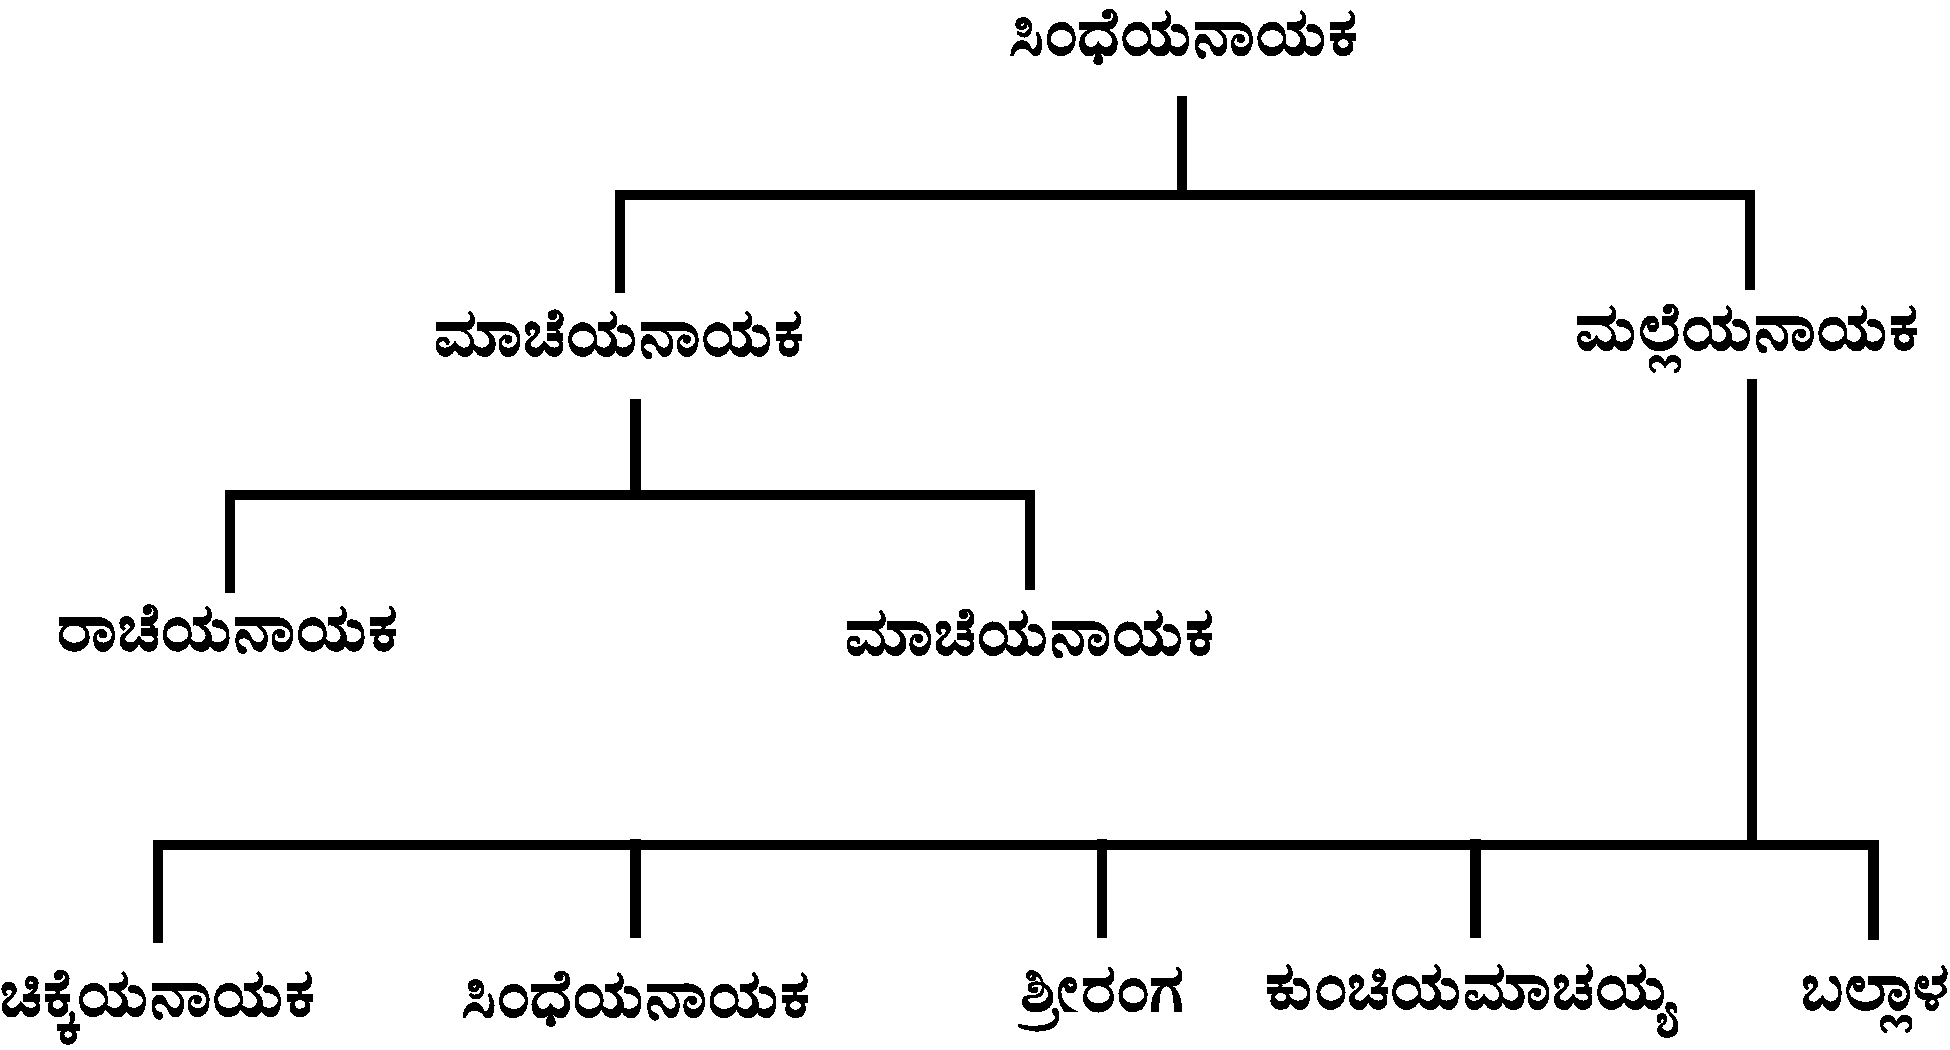
\includegraphics[scale=1.2]{images/chap3/chap3fig9.jpeg}
\end{figure}


\section*{ಮಹಾ ಪ್ರಭು\index{ಮಹಾ ಪ್ರಭು}/ಪ್ರಭು\index{ಪ್ರಭು ಗಾವುಂಡ (ಗಾವುಂಡರು) (ಗವುಡುಗಳು)}/ವಿಭುಗಳು\index{ವಿಭು}}

ಮಹಾ ಮಂಡಳೇಶ್ವರರು, ಮಹಾ ಸಾಮಂತರು, ಪ್ರಭು ಗಾವುಂಡರು, ಗಾವುಂಡರು, ಇವರು ಪ್ರಭು ವರ್ಗದವರೆಂದು, ಈ ಪ್ರಭು ವರ್ಗದವರ ನಡುವೆ ಇರುವ ಅಂತರ, ಅಧಿಕಾರ ವ್ಯಾಪ್ತಿಯನ್ನು ಈವರೆಗೆ ಸ್ಪಷ್ಟವಾಗಿ ಗುರುತಿಸಿಲ್ಲ ಎಂದು ವಿದ್ವಾಂಸರು ಅಭಿಪ್ರಾಯಪಟ್ಟಿದ್ದಾರೆ.\endnote{ ನಾಗಯ್ಯ, ಡಾ॥ ಜೆ.ಎಮ್., ಆರನೆಯ ವಿಕ್ರಮಾದಿತ್ಯನ ಶಾಸನಗಳು, ಪುಟ 151} ಮಹಾ ಪ್ರಭುಗಳು ಮಹಾ ಸಾಮಂತರಿಗೆ ಸಮಾನವಾಗಿಯೂ, ಪ್ರಭು ಅಥವಾ ವಿಭುಗಳು ಸಾಮಂತರಿಗೆ ಸಮಾನರಾಗಿಯೂ ಇದ್ದರೆಂದು ಹೇಳಬಹುದು. ಇಂತಹ ಅನೇಕ ಪ್ರಭುಗಳ ಉಲ್ಲೇಖ ಹೊಯ್ಸಳರ ಕಾಲದ ಶಾಸನಗಳಲ್ಲಿ ಕಂಡುಬರುತ್ತದೆ.

\textbf{ಮಹಾ ಪ್ರಭು (ಮಹಾಸಾಮಂತ) ಬಿಟ್ಟಿಗಾವುಂಡ\index{ಬಿಟ್ಟಿಗಾವುಂಡ} ಹಾಗೂ ಅವನ ವಂಶಸ್ಥರು (1200):} ಶ‍್ರೀಮನ್​ ಮಹಾಪ್ರಭು ಮೊಡವನಕೋಡಿಯ\index{ಮೊಡವನಕೋಡಿ} ಬಿಟ್ಟಿಗಾವುಡನು ಕತ್ತರಿಗಟ್ಟದ ವೃತ್ತಿಯನ್ನು\index{ಕತ್ತರಿಗಟ್ಟದ ವೃತ್ತಿ} ಆಳುತ್ತಿದ್ದನು. ಇವನ ಹೆಂಡತಿ ರಾಣಿಮುಖ ಜ್ಯೋತಿ \hbox{ದುಬಿ} ಗಾವುಂಡಿ\index{ದುಬಿ ಗಾವುಂಡಿ}. ಇವರ ಮಗ ಮಹಾಪ್ರಭು ಮಲ್ಲಿಯಣ್ಣ. ಕತ್ತರಿಗಟ್ಟ ನಾಡಿನ\index{ಕತ್ತರಿಗಟ್ಟ ನಾಡು} (ಕುರುಣೆಯನ) ಹಳ್ಳಿಯ\index{ಕುರುಣೆಯನ ಹಳ್ಳಿ} ತುರುಗಳನ್ನು ಬಬಿ ನಾಡಾಳ್ವರು\index{ಬಬಿ ನಾಡಾಳ್ವರು} ಎತ್ತಿಕೊಂಡು ಹೋಗಲು, ತಾನು ಹಿಂದೆಹಬ್ಬಿ (ಬೆನ್ನಟ್ಟಿ) ತಾಗಿ ತಳ್ತಿರಿದು ತುರುವನ್ನು ಮರಳಿಸಿ, ಮಲ್ಲಿಯಣ್ಣ\index{ಮಲ್ಲಿಯಣ್ಣ}, ಅವನ ತಮ್ಮ ಮಾರಗೌಡ\index{ಮಾರಗೌಡ}, ಮತ್ತು ಬ(ಭೈ)ರಯನಾಯಕ\index{ಭೈರಯನಾಯಕ} ಇವರುಗಳು, ಕೂರಯ ನಾಯಕನ\index{ಕೂರೆಯನಾಯಕ} ಬವರದಲ್ಲಿ ತಾಗಿ ಒಂದೇ ದಿನದಲಿ ಕೈಲಾಸ ಪ್ರಾಪ್ತರಾಗುತ್ತಾರೆ.\endnote{ ಎಕ 6 ಕೃಪೇ 111 ಮಡುವಿನಕೋಡಿ 1200 ಏಪ್ರಿಲ್​ 25} ಕೂರಯನಾಯಕನು ಬಾಚಿಯಹಳ್ಳಿಯ ಕಬ್ಬಾಹು ನಾಡಿನ ಮಹಾ ಸಾಮಂತನಾಗಿದ್ದುದು ನಮಗೆ ತಿಳಿದುಬರುತ್ತದೆ. ಅವನ ಕೈಕೆಳಗೆ ಈ ಕತ್ತರಿಘಟ್ಟದ ಪ್ರಭುಗಳು ಆಳುತ್ತಿದ್ದು, ಕೂರಯ ನಾಯಕನು ಹೂಡಿದ ಯುದ್ಧದಲ್ಲಿ ಅವನ ಪರವಾಗಿ ಹೋರಾಡಿರಬಹುದು.

ಮಡುಹಿನ ಕೋಡಿಯ\index{ಮಡುವಿನ (ಮಡವನ) ಕೋಡಿ (ಮಡುಹಿನ ಕೋಡಿ)} ಕತ್ತರಿಘಟ್ಟ ನಾಡಾಳುವ\index{ಕತ್ತರಿಘಟ್ಟ ನಾಡು} ಬಿಕೆಯ ನಾಯಕ\index{ಬಿಕೆಯ ನಾಯಕ} ಮತ್ತು ಅವನ ಹೆಂಡತಿ ಮಾಚವ್ವೆ\index{ಮಾಚವ್ವೆ} ಇವರ ಪ್ರಸ್ತಾಪ ಮಡುವಿನ ಕೋಡಿಯ ಇದೇ ಕಾಲದ ಇನ್ನೊಂದು ವೀರಗಲ್ಲಿನಲ್ಲಿದೆ.\endnote{ ಎಕ 6 ಕೃಪೇ 112 ಮಡುವಿನಕೋಡಿ 1200 ಏಪ್ರಿಲ್​ 25} ಮಹಾಪ್ರಭು ಮಲ್ಲಿಯಣ್ಣ\index{ಮಹಾಪ್ರಭು ಮಲ್ಲಿಯಣ್ಣ} ಮತ್ತು ಬಿಕೆಯ ನಾಯಕರು, ಬಿಟ್ಟಿ ಗಾವುಡನ ಮಕ್ಕಳಾಗಿರಬಹುದು. ಮಾಚವ್ವೆಯನ್ನೂ\index{ಮಾಚವ್ವೆ} ರಾಣಿಮುಖಜ್ಯೋತಿ\index{ರಾಣಿಮುಖಜ್ಯೋತಿ} ಎಂದು ಹೊಗಳಿರುವುದರಿಂದ ಬಿಕೆಯ ನಾಯಕನೂ ಕೂಡಾ ಮಹಾ ಪ್ರಭುವಾಗಿರಬಹುದು. ಈ ಶಾಸನದಲ್ಲೂ ಕೂಡಾ, ಅಗ್ರಹಾರ ಬಾಚಹಳ್ಳಿ\index{ಅಗ್ರಹಾರಬಾಚಹಳ್ಳಿ} ಶಾಸನೋಕ್ತರಾದ, ಕಬ್ಬಾಹು ನಾಡಿನ ಮಹಾ ಸಾಮಂತರಾಗಿದ್ದ ಬಾಚಿಯಹಳ್ಳಿಯ\index{ಬಾಚಹಳ್ಳಿ (ಬಾಚಿಯ - ಬಾಚೆಯಹಳ್ಳಿ)} ಮಲ್ಲೆಯನಾಯಕ ಮತ್ತು ಕೂರೆಯನಾಯಕ ಇವರ ಪ್ರಸ್ತಾಪವಿದೆ. ಇವರ ಜೊತೆ ಯಾವುದೋ ಹೋರಾಟದಲ್ಲಿ ಭಾಗವಹಿಸಿ ಮಲ್ಲಿಯಣ್ಣನು ಮಡಿದನೆಂದು ತೋರುತ್ತದೆ.

ಮುಂದೆ ಇದೇ ವಂಶದವರೇ ಮಹಾ ಪ್ರಭುಗಳಾಗಿ ಕ್ರಿ.ಶ.1346 ರಲ್ಲಿಯೂ ಕೂಡಾ ಕತ್ತರಿಗಟ್ಟದ ನಾಡನ್ನು ಆಳುತ್ತಿದ್ದರೆಂದು ತಿಳಿದುಬರುತ್ತದೆ.\endnote{ ಎಕ 6 ಕೃಪೇ 110 ಮಡುವಿನಕೋಡಿ 1346 ಅಕ್ಟೋಬರ್​ 25} ಈ ವೇಳೆಗೆ ವಿಜಯನಗರ ಸಾಮ್ರಾಜ್ಯ ಅಸ್ತಿತ್ವಕ್ಕೆ ಬಂದಿದ್ದರೂ ಅದರ ಉಲ್ಲೇಖ ಈ ಶಾಸನದಲ್ಲಿ ಇಲ್ಲದಿರುವುದು ಆಶ್ಚರ್ಯಕರ. ಕತ್ತರಿಗಟ್ಟದ ನಾಡಾಳ್ವ ಪ್ರಭು ಮೊಡವನಕೋಡಿಯ ಮಾಚೆಗವುಡ\index{ಮಾಚೆಗವುಡ} ಮತ್ತು ಅವನ ಪತ್ನಿ ರಾಣಿಮುಖಜ್ಯೋತಿ ಮಾದಗವುಡಿಯ\index{ಮಾದಗವುಡಿ} ಪುತ್ರ ಸಕಳಿಗವುಡನು\index{ಸಕಳಿಗವುಡ} ತನ್ನೂರಾದ ಕುರುಣೆಯನ ಹಳ್ಳಿಯನ್ನು\index{ಕುರುಣೆಯನ ಹಳ್ಳಿ} ಶತ್ರುಗಳು ಬಂದು ದಳದಳವಾಗಿ ಮುತ್ತಿದಲ್ಲಿ ಹೋರಾಡಿ ಮಡಿಯುತ್ತಾನೆ. ಇವನ ಜೊತೆ ಮಲ್ಲಿಯಣ್ಣ, ಕೂರೆಯನಾಯಕ, ಬಿಂಮನಾಯಕ ಇವರುಗಳು ಮಡಿಯುತ್ತಾರೆ. ಬಹುಶಃ ಮಲ್ಲಿಯಣ್ಣ ಮುಂತಾದವರು ಇವನ ತಮ್ಮಂದಿರಿರಬಹುದು. ಕಾರಣ ಈ ವಂಶದ ಮೂಲಪುರುಷನ ಹೆಸರು ಮಲ್ಲಿಯಣ್ಣ ಎಂದಿದೆ. ಸಕಳಿಗವುಡನನ್ನು ಶಾಸನವು \textbf{“ಶ‍್ರೀಮನ್ ಮಹಾಸಾಮಂತ ಬಿರುದರಗೋವ ಸತ್ಯರಾಧೇಯ ಸೌಜನಬಾಂಧವ ಆಶ್ರಿತಜನಕಲ್ಪವೃಕ್ಷ, ಗೋತ್ರಚಿಂತಾಮಣಿ, ಬಂಧುಜನಧವಳ, ತಂದೆಯಗಂಧವಾರಣ\general{\break } ಅಣ್ಣನಂಕುರ”} ಎಂದು ಹೊಗಳಿದೆ. ಪ್ರಭುವಾಗಿದ್ದವನನ್ನು ಮಹಾಸಾಮಂತ\index{ಮಹಾಸಾಮಂತ} ಎಂದು ಹೇಳಿದ್ದು ಎರಡು ಹುದ್ದೆಗೂ ಅಂತಹ ವ್ಯತ್ಯಾಸ ಇರಲಿಲ್ಲವೆಂದು ಹೇಳಬಹುದು. ಕುರುಣೆಯನ ಹಳ್ಳಿಯು ಮಡುವಿನ ಕೋಡಿಗೆ ಸಮೀಪದಲ್ಲಿರುವ ಇಂದಿನ ಕುರ್ಣೇನ ಹಳ್ಳಿಯಾಗಿದೆ\index{ಕುರ್ಣೇನ ಹಳ್ಳಿ}. ಇವರ ವಂಶ ವೃಕ್ಷವನ್ನು ಈ ಕೆಳಗಿನಂತೆ ಕಟ್ಟಿಕೊಡಬಹುದು.

\begin{figure}[H]
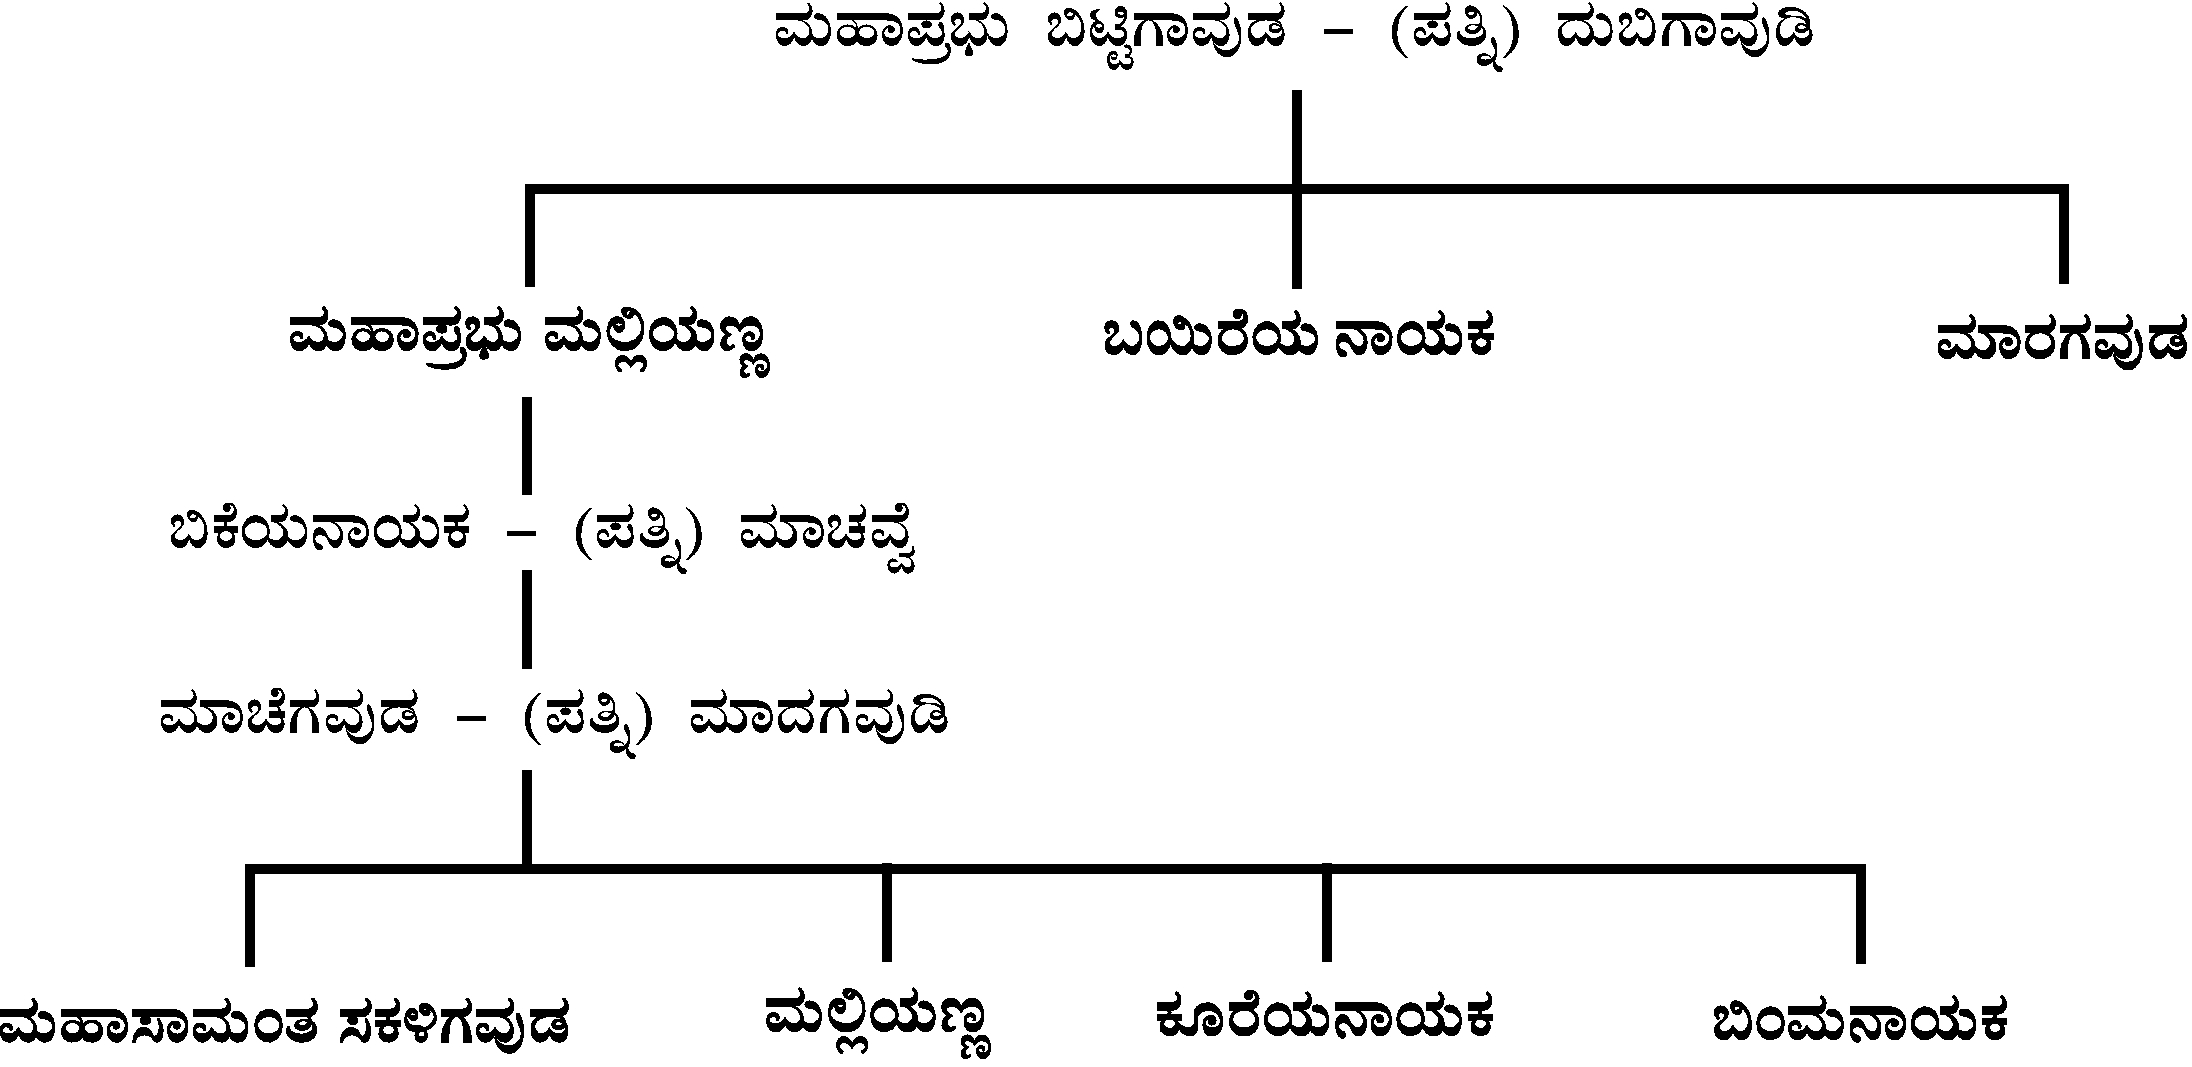
\includegraphics[scale=.15]{images/chap3/chap3fig10.jpeg}
\end{figure}

\textbf{ಮಹಾಪ್ರಭು\index{ಮಹಾಪ್ರಭು} ಮಾದಿರಾಜ\index{ಮಾದಿರಾಜ} (1144):} ಶ‍್ರೀಕರಣದ ಮಾಧವ ಅಥವಾ ಮಾದಿರಾಜನನ್ನು ಬೋಗಾದಿ\index{ಬೋಗಾದಿ} ಶಾಸನವು ಶ‍್ರೀಮನ್\-​ಮಹಾಪ್ರಭು ಎಂದು ಕರೆದಿದೆ. ಅದೇ ಶಾಸನದಲ್ಲಿ ಇನ್ನೊಂದು ಕಡೆ ಮಾದಿರಾಜ ವಿಭು ಎಂದು ಹೇಳಿದೆ. ವಿಭು, ಪ್ರಭು ಒಂದೇ ಹುದ್ದೆ ಇರಬಹುದು. ಇವನ ಗುರುಗಳ ಅನ್ವಯವನ್ನು, ಇವನ ವಂಶಾವಳಿಯನ್ನೂ ಶಾಸನವು ನೀಡಿದ್ದು ಬಹುಭಾಗ ತ್ರುಟಿತವಾಗಿದೆ. ವಿಭು ಪದ್ಮನಾಭನ\index{ವಿಭು ಪದ್ಮನಾಭ} ಉಲ್ಲೇಖವೂ ಇದರಲ್ಲಿದ್ದು, ವಿಭು ಮಾದಿರಾಜನು ಇವನ ಮಗನಿರಬಹುದು. ಮಾಚಿರಾಜನು ಕಟ್ಟಿಸಿದ ಶ‍್ರೀಕರಣ ಜಿನಾಲಯಕ್ಕೆ\index{ಶ‍್ರೀಕರಣ ಜಿನಾಲಯ} ಹೊಯ್ಸಳದೇವರು ಅಂದರೆ ವಿಷ್ಣುವರ್ಧನನು\index{ವಿಷ್ಣುವರ್ಧನ (ದೇವರು) (ಹೊಯ್ಸಳರ ದೊರೆ)} ತುಂಗಭದ್ರಾ\index{ತುಂಗಭದ್ರಾ (ನದಿ-ತೀರ್ಥ-ತೀರ)} ತೀರಲ್ಲಿದ್ದಾಗ, ದತ್ತಿಗಳನ್ನು ಬಿಟ್ಟನೆಂದು ಹೇಳಿದೆ.\endnote{ ಎಕ 7 ನಾಮಂ 183 ಬೋಗಾದಿ 1144}

\textbf{ವಿಭು\index{ವಿಭು} ಮಾಚಿರಾಜ\index{ಮಾಚಿರಾಜ} (1173):} ವಿಭು(ಪ್ರಭು) ಮಾಚಿರಾಜನ ಉಲ್ಲೇಖ ಬೋಗಾದಿ\index{ಬೋಗಾದಿ} ಶಾಸನದಲ್ಲಿ ಬರುತ್ತದೆ. ಈತನು ಮೊದಲಿಗೆ (1173) ಸಾಮಂತನಾಗಿರಬಹುದು.\endnote{ ಎಕ 7 ನಾಮಂ 181 ಬೋಗಾದಿ 1173} ಮಹಾಪ್ರಧಾನ ಸರ್ವಾಧಿಕಾರಿ ಹೆಗ್ಗಡೆ ಬಲ್ಲಯ್ಯನು\index{ಹೆಗ್ಗಡೆ ಬಲ್ಲಯ್ಯ} ಮಾಚಿರಾಜನ ಮಾವ. ಮಾಚಿರಾಜನು ಬಲ್ಲಾಳನ \textbf{“ಅಗಣ್ಯಪುಣ್ಯವೇ ಮಾನಸರೂಪವಾದುದೋ”} ಎಂಬಂತೆ ಇದ್ದನೆಂದು ಶಾಸನವು ಹೊಗಳಿದೆ.

\textbf{ಚುಂಚನಕೋಟೆ\index{ಚುಂಚನಕೋಟೆ} ಪ್ರಭು ರಾಮೆಯನಾಯ್ಕ\index{ರಾಮೆಯನಾಯ್ಕ} (1205):} ಇಮ್ಮಡಿ ಬಲ್ಲಾಳನ ಕಾಲದಲ್ಲಿ, ಚುಂಚನಕೋಟೆಯ ಪ್ರಭು \textbf{“ಸತ್ಯಕೆ ತಪ್ಪುವನಾಯಕರ ಗಂಡ, ಮರೆವೊಕ್ಕಡೆಕಾವ ಮಾರಥ, ಗಂಡಗೂಳಿ, ಕೂಟದೊಳು ಕೂಡುವನಾಯಕರ ಗಂಡ, ಸಾರೆಯ್ಕ ಮಗ ರಾಮೆಯನಾಯಕನು ಬೆಲುಹೂರಲಿ\index{ಬೆಲುಹೂರು} ಎಡವಾರಯ ರಾಚಯ್ಯನಾಯಕನ ಕೂಡೆ ಕಾದಿ”} ಸತ್ತನು. ಆಗ ಬಹುಶಃ ಇವನ ಪುತ್ರರೋ ಅಥವಾ ತಮ್ಮಂದಿರೋ ಆದ ಹಿರಿಯ ಗೋವಿ ನಾಯಕ ಮತ್ತು ಚಿಕ್ಕಮಾಯಿ ನಾಯಕ ಇವರುಗಳು ಬೀರಗಲ್ಲನ್ನು\index{ಬೀರಗಲ್ಲು} ಎತ್ತಿಸಿದರೆಂದು ತಿಳಿದುಬರುತ್ತದೆ.\endnote{ ಎಕ 7 ನಾಮಂ 111 ಚುಂಚನಹಳ್ಳಿ 1205}

\section*{ಶ‍್ರೀಮನ್ಮಹಾಪ್ರಧಾನ ದಂಡನಾಯಕರು\index{ಶ‍್ರೀಮನ್ಮಹಾಪ್ರಧಾನ ದಂಡನಾಯಕರು}\enginline{-} ಸಚಿವರು\index{ಸಚಿವರು}\enginline{-} ಮಂತ್ರಿಗಳು\index{ಮಂತ್ರಿಗಳು}}

\textbf{ಹೊಯ್ಸಳರ ಕಾಲದಲ್ಲಿ ಪಂಚಪ್ರಧಾನ ಪದ್ಧತಿ ಜಾರಿಯಲ್ಲಿತ್ತು. ನಾರಸಿಂಘ ಚತುರ್ವೇದಿ ಮಂಗಲಕ್ಕೆ\index{ನಾರಸಿಂಘ (ನಾರಸಿಂಹ) ಚತುರ್ವೇದಿ ಮಂಗಲ} ಸೇರಿದ ವೈಜನಾಥ ದೇವರ ದೇವಾಲಯಕ್ಕೆ ಬಿಟ್ಟಿದ್ದ, ಹುಲಗೂರು ದತ್ತಿಯನ್ನು ಪುನರುಜ್ಜೀವನಗೊಳಿಸುವಂತೆ ಬಿಟ್ಟೀದೇವನು(ಇಮ್ಮಡಿಬಲ್ಲಾಳ) ಬೆಸಸಲು, ಶ‍್ರೀಮನು ಮಹಾಪ್ರಧಾನನು ಆ ಬೆಸನನ್ನು ಕೈಕೊಂಡು ಹೆಗ್ಗಡೆಗೆ ಬೆಸೆಸಿದನು. ಆಗ ಪಂಚಮಹಾಪ್ರಧಾನರ\index{ಪಂಚಮಹಾಪ್ರಧಾನ} ದಿವ್ಯ ವಚನದಂತೆ ಈ ದತ್ತಿಯನ್ನು ಪುನಃ ಬಿಡಲಾಯಿತೆಂದು ತಿಳಿದುಬರುತ್ತದೆ.}\endnote{ ಎಕ 7 ಮವ 41 ಕೊನ್ನಾಪುರ 1192} ರಾಜ್ಯದ ಆಡಳಿತ ವ್ಯವಸ್ಥೆ ರಾಜನಿಂದ ಹೆಗ್ಗಡೆಯವರೆಗೆ ಯಾವರೀತಿ ನಡೆಯುತ್ತಿತ್ತು ಎಂಬುದನ್ನು ಇದು ಸೂಚಿಸುತ್ತದೆ. \textbf{ಪಂಚಮಹಾಪ್ರಧಾನರೆಂದರೆ ಸಂಧಿವಿಗ್ರಹಿ\index{ಸಂಧಿವಿಗ್ರಹಿ}, ಶ‍್ರೀಕರಣಾಧಿಕಾರಿ\index{ಶ‍್ರೀಕರಣಾಧಿಕಾರಿ}, ಹಿರಿಯಭಂಡಾರಿ\index{ಹಿರಿಯಭಂಡಾರಿ}, ಸೇನಾಪತಿ\index{ಸೇನಾಪತಿ} ಮತ್ತು ಮಹಾಪಸಾಯಿತ\index{ಮಹಾ ಪಸಾಯ್ತ (ಪಸಾಯಿತ, ಪಸಾಯತ)ರು}} ಎಂಬುದು ವಿದ್ವಾಂಸರ ಅಭಿಪ್ರಾಯ.\endnote{ ಕೃಷ್ಣರಾವ್​, ಎಂ.ವಿ., ಕರ್ನಾಟಕ ಇತಿಹಾಸ ದರ್ಶನ, ಪುಟ 908} ಶ‍್ರೀಮನ್ಮಹಾಪ್ರಧಾನ ಎಂಬುದು ಪರಮೋಚ್ಛ ಅಧಿಕಾರದ ಹುದ್ದೆ. ಇವರು ಸಾಮಾನ್ಯವಾಗಿ ದಂಡನಾಯಕರೂ ಆಗಿರುತ್ತಿದ್ದರು. ಕೆಲವು ಶ‍್ರೀಮನ್ಮಹಾಪ್ರಧಾನ ದಂಡನಾಯಕರನ್ನು ಮಾತ್ರ ಶಾಸನಗಳು ಮಂತ್ರಿ, ಸಚಿವ ಎಂದು ಕರೆದಿವೆ. ಪಂಚ ಮಹಾಪ್ರಧಾನ\-ರಲ್ಲಿ ಇವರೇ ಮೊದಲಿಗರೆಂದು ಹೇಳಬಹುದು. "ಮಹಾಪ್ರಧಾನ ಅಥವಾ ಮಹಾಮಾತ್ಯನು ಮಂತ್ರಿಮಂಡಲದ ಮುಖ್ಯಸ್ಥನೆಂದು ಭಾವಿಸಬಹುದು" ಎಂದು ಡಾ. ಎಂ. ಚಿದಾನಂದಮೂರ್ತಿಯವರು ಹೇಳಿದ್ದಾರೆ.\endnote{ ಚಿದಾನಂದ ಮೂರ್ತಿ, ಡಾ. ಎಂ. ಕ. ಶಾ. ಸಾಂ. ಅ., ಪುಟ 331} ಆದರೆ “ಶಾಸನ\-ಗಳಲ್ಲಿ ಬಹುಮಟ್ಟಿಗೆ ತಪ್ಪದೇ ಬರುವ ಮಹಾಮಾತ್ಯಪದವಿ\index{ಮಹಾಮಾತ್ಯ} ವಿರಾಜಮಾನ ಎಂಬು ಪದವು, ಗೌರವಸೂಚಿ ಪದವಿಯೆಂದು ಸ್ಪಷ್ಟಪಡಿಸುತ್ತದೆಂದು ಎಂದು ಡಾ. ನಾಗಯ್ಯನವರು ಹೇಳುತ್ತಾರೆ.\endnote{ ನಾಗಯ್ಯ ಡಾ॥ ಜೆ.ಎಂ., ಆರನೆಯ ವಿಕ್ರಮಾದಿತ್ಯನ ಶಾಸನಗಳು-ಒಂದು ಅಧ್ಯಯನ, ಪುಟ 277, 279}

ಹೊಯ್ಸಳರ ಶಾಸನಗಳನ್ನು ಪರಿಶೀಲಿಸಿದಾಗ ಮಹಾಮಾತ್ಯ ಎಂಬ ಪದವಿಯ ಬಳಕೆ ಹೆಚ್ಚಾಗಿ ಕಂಡುಬರುವುದಿಲ್ಲ. ಮಹಾಪ್ರಧಾನ ದಂಡನಾಯಕ ಎಂಬ ಹುದ್ದೆಯು ಹೆಚ್ಚಾಗಿ ಕಂಡುಬಂದಿದ್ದು, ಇವರಲ್ಲಿ ಕೆಲವರಿಗೆ ಸರ್ವಾಧಿಕಾರಿ, ಮಹಾಪಸಾಯ್ತ, ದಂಡದಧಿಷ್ಠಾಯಕ, ಬಾಹತ್ತರ ನಿಯೋಗಾಧಿಪತಿ, ಮನೆವೆರ್ಗ್ಗಡೆ, ಹುದ್ದೆಗಳನ್ನು ಹೆಚ್ಚುವರಿಯಾಗಿ ನೀಡಿದೆ.\endnote{ \engfoot{Radha Patel, Dr.M., Life and Times of Narasimha III, pp. 39}} ಇನ್ನು ಕೆಲವರನ್ನು ಕೇವಲ ದಂಡನಾಯಕರು, ಸೇನಾನಾಯಕರು ಎಂದು ಕರೆದಿದೆ. ಅವರನ್ನು ಎಲ್ಲೂ ಮಹಾಪ್ರಧಾನರೆಂದು ಕರೆದೇ ಇಲ್ಲ. ಮಹಾಪ್ರಧಾನ ದಂಡನಾಯಕರ ಹುದ್ದೆಯನ್ನು ಹೊರತುಪಡಿಸಿ, ದಂಡನಾಯಕ, ಶ‍್ರೀಕರಣದ ಹೆಗ್ಗಡೆ, ಸುಂಕದ ಹೆಗ್ಗಡೆ, ಮನೆವೆಗ್ಗಡೆ, ಪಸಾಯ್ತ, ಮಹಾ ಪಸಾಯ್ತ, ಭಂಡಾರಿ, ಹಿರಿಯಭಂಡಾರಿ, ಹಡೆವಳ, ಹಿರಿಯಹಡೆವಳ ಎಂಬ ಅನೇಕ ಹುದ್ದೆಗಳನ್ನು ಕಾಣಬಹುದು. ಈ ಹುದ್ದೆಗಳಿಗೆ ಎಲ್ಲಿಯೂ ಮಹಾ ಪ್ರಧಾನ ಎಂಬ ವಿಶೇಷಣವನ್ನು ನೀಡಿಲ್ಲ. ಅಂದಮೇಲೆ ಮಹಾ ಪ್ರಧಾನ ಹುದ್ದೆಯು ಮುಖ್ಯಮಂತ್ರಿಯ ಹುದ್ದೆಯಾಗಿದ್ದು, ಬಹಳ ಜವಾಬ್ದಾರಿಯುತವಾದ ದೊಡ್ಡ ಹುದ್ದೆಯಾಗಿತ್ತೆಂದು ಹೇಳಬಹುದು. ಕೆಲವರಿಗೆ ಮಾತ್ರ ಅವರವರ ಯೋಗ್ಯತೆಗೆ ತಕ್ಕಂತೆ ಮಹಾಪ್ರಧಾನ ಪದವಿಯ ಜೊತಗೆ, ದಂಡನಾಯಕ ಹಾಗೂ ಇತರ ಅಧಿಕಾರದ ಪದವಿಗಳನ್ನು ನೀಡಿರುವುದು ಶಾಸನಗಳಿಂದ ಸ್ಪಷ್ಟವಾಗಿ ತಿಳಿದುಬರುತ್ತದೆ. ಗಂಗರಾಜನು ಮೊದಲು ದಂಡಾಧೀಶ ಅಥವಾ ದಂಡನಾಯಕನಾಗಿ, ಆಮೇಲೆ ಮಹಾಪ್ರಧಾನ ದಂಡನಾಯಕನಾಗಿ, ಮುಂದೆ ಮಹಾ ಸಾಮಂತ ಪದವಿಗೇರಿರುವುದು ಶಾಸನಗಳಲ್ಲಿ ಕಂಡುಬರುತ್ತದೆ.

ಹೊಯ್ಸಳರ ಕಾಲದ ಬಹುತೇಕ ಮಹಾಪ್ರಧಾನರು, ದಂಡನಾಯಕರು ಮಂಡ್ಯ ಜಿಲ್ಲೆಯ ಶಾಸನಗಳಲ್ಲಿ ಕಂಡು\-ಬರುತ್ತಾರೆ. ಅವರಲ್ಲಿ ಕೆಲವರು ಮಾತ್ರ ಜಿಲ್ಲೆಯ ಅಕ್ಕಪಕ್ಕದ, ಶ್ರವಣಬೆಳಗೊಳ, ಹಾಸನ, ಮೈಸೂರು ಜಿಲ್ಲೆಯ ಶಾಸನಗಳಲ್ಲಿ ಕಂಡು ಬರುತ್ತಾರೆ. ಇನ್ನು ಕೆಲವರಂತೂ ಜಿಲ್ಲೆಯ ಶಾಸನಗಳನ್ನು ಬಿಟ್ಟರೆ ಅಕ್ಕಪಕ್ಕದ ಅಥವಾ ಬೇರೆ ಜಿಲ್ಲೆಯ ಶಾಸನಗಳಲ್ಲಿ ಕಂಡುಬರುವುದಿಲ್ಲ. ಆದಕಾರಣ ಇಂತಹ ಮಹಾಪ್ರಧಾನ ದಂಡನಾಯಕರು, ಅಧಿಕಾರಿಗಳು, \textbf{ಮಂಡ್ಯ ಜಿಲ್ಲೆಯ ಪ್ರದೇಶದವರೇ ಆಗಿದ್ದು, ತಮ್ಮ ತಮ್ಮ ಊರನ್ನೇ ತಮ್ಮ ಕಾರ್ಯಕ್ಷೇತ್ರವನ್ನಾಗಿ ಮಾಡಿಕೊಂಡು, ದೇವಾಲಯಗಳ ನಿರ್ಮಾಣ, ಕೆರೆಕಟ್ಟೆಗಳ ನಿರ್ಮಾಣ ಮೊದಲಾದ ಜನೋಪಕಾರಿ ಕೆಲಸಗಳನ್ನು ಮಾಡುತ್ತಿದ್ದರೆಂದು ಹೇಳಬಹುದು.}

\textbf{ಶ‍್ರೀಮನ್ಮಹಾಪ್ರಧಾನ\index{ಶ‍್ರೀಮನ್ಮಹಾಪ್ರಧಾನ} ಹಿರಿಯ ದಂಡನಾಯಕ ಗಂಗರಾಜ\index{ಗಂಗರಾಜ}(1115\general{\enginline{-}}1123):} ಗಂಗರಾಜನು ಹೊಯ್ಸಳರ ಅತ್ಯಂತ ಪ್ರಮುಖ ದಂಡನಾಯಕ. ಈತನು ವಿಷ್ಣುವರ್ಧನಿಗಾಗಿ ತಲಕಾಡನ್ನು ಗೆದ್ದುಕೊಟ್ಟನು. ಚೋಳರನ್ನು ತಲಕಾಡಿನಿಂದ ಓಡಿಸಿ ಅವರ ನೂರು ವರ್ಷಗಳ ಆಳ್ವಿಕೆಯನ್ನು ಕೊನೆಗೊಳಿಸಿದನು. ಈ ಘಟನೆ ಕ್ರಿ.ಶ.1115\enginline{-}16ರಲ್ಲಿ ನಡೆದಿರುವ ಸಾಧ್ಯತೆ ಇದೆ. ಈತನು ವಿಷ್ಣುವರ್ಧನನ \textbf{ಮಹಾಸಾಮಂತಾಧಿಪತಿ ಶ‍್ರೀಮನ್ಮಹಾಪ್ರಧಾನಿ ಮಂತ್ರಿಮಾಣಿಕ್ಯ ಹಾಗೂ ಪಿರಿಯ ದಂಡನಾಯಕನಾಗಿದ್ದನೆಂದು\index{ಪಿರಿಯ ದಂಡನಾಯಕ}}ತಿಳಿದುಬರುತ್ತದೆ.\endnote{ ಎಕ 2 ಶ್ರಬೆ 156 ಚಿಕ್ಕಬೆಟ್ಟ (ಎರಡುಕಟ್ಟೆ ಬಸದಿ) 1115 ಡಿಸೆಂಬರ್​ 2} ಬಹುಶಃ ಈತನು \textbf{ಮಹಾಸಾಮಂತನಾಗಿ} ಕಲ್ಕುಣಿ ನಾಡನ್ನು\index{ಕಲುಕಣಿ (ಕಲಿಕಣಿ-ಕಲ್ಕಣಿ-ಕಲ್ಕುಣಿ-ಕಲುಕರೆ) ನಾಡು} ಆಳುತ್ತಿದ್ದಿರ\-ಬಹುದು. ಈತನಿಗೆ ದ್ರೋಹಘರಟ್ಟ ಎಂಬ ಬಿರುದಿತ್ತು.

ವಿಷ್ಣುವರ್ಧನನ ವಿಜಯಗಳನ್ನು ವಿವರವಾಗಿ ಮೊದಲಬಾರಿಗೆ ತಿಳಿಸುವ ಬೇಲೂರು ಪ್ರಶಸ್ತಿ ಶಾಸನವು ಕ್ರಿ.ಶ.1117 ಮಾರ್ಚ್ 10 ರಂದು ಹೊರಟಿದೆ. \textbf{“ತಳಕಾಡಂ ಗಂಗರಾಜ್ಯಕ್ಕೆ ತಾಂ ಮೊದಲಾದಂ ಯದುವಂಶವರ್ಧನಕರಂ ಶ‍್ರೀವಿಷ್ಣು\-ಭೂಪಾಳಕಂ\index{ಶ‍್ರೀವಿಷ್ಣುಭೂಪಾಳಕಂ}” }ಎಂದು ಹೇಳಿದೆ.\endnote{ ಎಕ 9 ಬೇಲೂರು 16 ಬೇಲೂರು} ವಿಷ್ಣುವರ್ಧನನು ಚೋಳರ ಮೇಲಿನ ವಿಜಯದ ಜ್ಞಾಪಕಾರ್ಥವಾಗಿ, ಬೇಲೂರಿನಲ್ಲಿ ವಿಜಯನಾರಾಯಣ\index{ವಿಜಯನಾರಾಯಣ} ಮೊದಲಾದ ದೇವರನ್ನು ಪ್ರತಿಷ್ಠಾಪಿಸಿ, ವಿಜಯೋತ್ಸವವನ್ನು ಆಚರಿಸಿದ ನಂತರ, ಗಂಗರಾಜನು ತಲಕಾಡು ವಿಜಯಕ್ಕಾಗಿ ಅವನಿಂದ ದತ್ತಿಗಳನ್ನು ಪಡೆದಿರಬಹುದು. ಆದುದರಿಂದಲೇ ಬೇಲೂರು ಶಾಸನದ ನಂತರವಷ್ಟೇ, ಅರೆತಿಪ್ಪೂರು\index{ಅರೆತಿಪ್ಪೂರು}, ಕಂಬದಹಳ್ಳಿ\index{ಕಂಬದಹಳ್ಳಿ}, ಸಾಣೆಹಳ್ಳಿ\index{ಸಾಣೆಹಳ್ಳಿ}, ಶ್ರವಣಬೆಳಗೊಳ\index{ಶ್ರವಣಬೆಳಗೊಳ} ಶಾಸನಗಳು ಹೊರಟಿವೆ.

ಕ್ರಿ.ಶ.1117 ಡಿಸೆಂಬರ್​ 15ರ ಅರೆತಿಪ್ಪೂರು ಶಾಸನವು ಗಂಗರಾಜನು ತಲಕಾಡನ್ನು ಗೆದ್ದುಕೊಟ್ಟ ಬಗೆಯನ್ನು ವಿವರವಾಗಿ ಬಣ್ಣಿಸುತ್ತದೆ.\endnote{ ಎಕ 7 ಮ 54 ತಿಪ್ಪೂರು 1117} ಈ ಶಾಸನದಲ್ಲಿ ಗಂಗರಾಜನ ವಂಶಾವಳಿಯನ್ನು ನೀಡಲಾಗಿದೆ. ಮಾರಯ್ಯ\index{ಮಾರಯ್ಯ} ಮತ್ತು ಮಾಕಣಬ್ಬೆಯರ\index{ಮಾಕಣಬ್ಬೆ} ಪುತ್ರ ಏಚಿರಾಜ\index{ಏಚಿರಾಜ}. ಈ ಏಚಿರಾಜನ ಹೆಂಡತಿ ಪೋಚಿಕಬ್ಬೆ\index{ಪೋಚಿಕಬ್ಬೆ}. ಇವರ ಪುತ್ರ ಶ‍್ರೀಮನ್ಮಹಾಪ್ರಧಾನ ದಂಡನಾಯಕ ದ್ರೋಹಘರಟ್ಟ\index{ದ್ರೋಹಘರಟ್ಟ} ಗಂಗರಾಜ. ಚೋಳನ ಸಾಮಂತ ಆದಿಯಮನು \textbf{“ತಲಕಾಡ\index{ತಲಕಾಡು} ಬೀಡಿನಲ್ಲಿ ಪಡಿಯಿಪ್ಪಂತೆ”} ಇದ್ದನಂತೆ. ಆಗ ಗಂಗರಾಜನು ತಲಕಾಡನ್ನು ಬಿಟ್ಟುಕೊಡಲು ಹೇಳಿ ಕಳುಹಿಸಿರಬಹುದು. ಅದಕ್ಕೆ ಆದಿಯಮನು\index{ಆದಿಯಮ} ಚೋಳಕೊಟ್ಟ ನಾಡನ್ನು ಕೊಡದೇ ಯುದ್ಧಮಾಡಿ ಜಯಿಸಿಕೊಳ್ಳಿ ಎಂದು ಹೇಳಿಕಳುಹಿಸಿದನಂತೆ.

\begin{verse}
\textbf{ಇತ್ತಣ ಭೂಮಿಭಾಗದೊಳದನ್ಯರದೇಕೆ ಭವತ್ಪ್ರತಾಪ ಸಂ} \\\textbf{ಪತ್ತಿಯ ವರ್ಣನಾ ವಿಧಿಗೆ ಗಂಗಚಮೂಪಂ ವಿಜಗೀಷುವೃತ್ತಿಯಿಂ} \\\textbf{ದೆತ್ತಿದ ನಿನ್ನ ಕೈಯ ನಿಸಿತಾಸಿಯ ತಾಮೊನೆಬೆನ್ನಬಾರನೆ} \\\textbf{ತ್ತುತ್ತಿರೆ ಪೋಗಿ ಕಂಚಿಗುರಿಯಪ್ಪನಮೋಡಿದ ದಾಮನೆಯ್ದನೆ}
\end{verse}

ಗಂಗರಾಜನು ಸೈನ್ಯದ ಹೊಡೆತಕ್ಕೆ ಬೆನ್ನಚರ್ಮವೇ ಎದ್ದುಹೋಗಲು ಆದಿಯಮನು ಕಂಚಿಯನ್ನೇ ಗುರಿಯನ್ನಾಗಿಸಿ\-ಕೊಂಡು ಓಡಿಹೋದನಂತೆ. ಅದನ್ನು ನೋಡಿ ಅವನ ದಂಡನಾಯಕನಾಗಿರಬಹುದಾದ ನರಸಿಂಹವರ್ಮನೂ “ಆದಿಯಮ\-ನೋಡಿದೋಟ ಮನೆರ್ದೋಡಿಸುತಂ ನರಸಿಂಹವರ್ಮ್ಮನೋಡಿದ”. \textbf{“ವೊಂದೆ ಮೆಯ್ಯೊಳೆಯ್ದಿ ನರಸಿಂಗವರ್ಮ\index{ನರಸಿಂಗವರ್ಮ} ಮೊದಲಾದ ಚೋಳನ ಸಾಮಂತರೆಲ್ಲರಂ ಬೆಂಕೊಂಡು ನಾಡಾದುದೆಲ್ಲವಮನೇಕಚ್ಛತ್ರಂ ಮಾಡಿ ಕುಡೆ ಕೃತಜ್ಞಂ ಬಿಷ್ಣುನೃಪತಿ ಮೆಚ್ಚಿದೆಂ ಬೇಡಿಕೊಳ್ಳಿಮೆನೆ ಅವನಿಪನೆನಗಿತ್ತಪನೆಂದವರಿವರವೊಲುಳಿದ ವಸ್ತುವಂ ಬೇಡದೆ ಭೂಭುವನಂ ಬಣ್ಣಿಸೆ ತಿಪ್ಪೂರ ವೃತಿಯಂ ಪಡೆದಂ\general{\break } ಜಿನಾರ್ಚನಲುಬ್ಧಂ}” ಎಂದು ತಿಪ್ಪೂರು ಶಾಸನ ವರ್ಣಿಸಿದೆ. ಕೃತಜ್ಞನಾದ ವಿಷ್ಣುವರ್ಧನನು ಮೆಚ್ಚಿದೆ ಏನುಬೇಕಾದರೂ ಬೇಡಿಕೋ ಎಂದಾಗ, ರಾಜನು ಹೇಗಿದ್ದರೂ ಕೊಡುತ್ತಾನೆ ಎಂದು ಅವರಿವರಂತೆ ಉಳಿದ ವಸ್ತುವನ್ನು ಬೇಡದೆ, ತಿಪ್ಪೂರ ವೃತ್ತಿಯನ್ನು\index{ತಿಪ್ಪೂರ ವೃತ್ತಿ} ಬೇಡಿ ತಮ್ಮ ಗುರುಗಳಾದ ಮೇಘಚಂದ್ರಸಿದ್ಧಾಂತ ದೇವರ ಕಾಲನ್ನು ತೊಳೆದು ದತ್ತಿಯಾಗಿ ಬಿಟ್ಟನು.\endnote{ ಎಕ 6 ಕೃಪೇ 60 ನಾಗರಘಟ್ಟ 12ನೇ ಶ.}

ಇದೇ ಘಟನೆಯನ್ನು ಕ್ರಿ.ಶ.1118ರ ನಾಗಮಂಗಲ ತಾಲ್ಲೂಕಿನ ಕಂಬದಹಳ್ಳಿ ಶಾಸನವೂ ಹೇಳಿದ್ದು, \textbf{“ಶ‍್ರೀಮನ್ಮಹಾ\-ಪ್ರಧಾನಿ ದ್ರೋಹಘರಟ್ಟ ಪಿರಿಯ ದಂಡನಾಯಕ ಗಂಗರಾಜ\index{ಗಂಗರಾಜ} ತಳೆಕಾಡಂ ಕೊಳುವಲ್ಲಿ ಮುಂಗೊಳ ಬೇಡಿಕೊಂಡು ಗೆಲ್ದಡೆ ಮೆಚ್ಚಿದೆಂ ಬೇಡಿಕೊಳ್ಳೆನೆ ಶ‍್ರೀ ಬಿಂಡಿಗನವಿಲೆಯ ತೀರ್ಥಕ್ಕೆ ತಳವ್ರಿತ್ತಿಯಂ ಬೇಡೆ ಶ‍್ರೀ ವಿಷ್ಣುವರ್ಧನ ಹೊಯ್ಸಳ ದೇವರು ಕಾರುಣ್ಯಂಗೆಯ್ದು ಕೊಡೆ” }ಅದನ್ನು ಶುಭಚಂದ್ರ ಸಿದ್ಧಾಂತ ದೇವರಿಗೆ ದತ್ತಿಯಾಗಿ ಬಿಟ್ಟನೆಂದು ಹೇಳಿದೆ.\endnote{ ಎಕ 7 ನಾಮಂ 33 ಕಂಬದಹಳ್ಳಿ 1118}

ತೇದಿಯಿಲ್ಲದ ಶ್ರವಣಬೆಳಗೊಳ\index{ಶ್ರವಣಬೆಳಗೊಳ} ಶಾಸನವೂ ಗಂಗರಾಜನು ತಲಕಾಡನ್ನು ಗೆದ್ದುಕೊಟ್ಟದ್ದಕ್ಕಾಗಿ, ಗೋವಿಂದವಾಡಿಯನ್ನು\index{ಗೋವಿಂದವಾಡಿ} ಜಿನಾರ್ಚನೆಗೆ ದತ್ತಿಪಡೆದು, ಗೊಮ್ಮಟದೇವನಿಗೆ ಸುತ್ತಾಲಯವನ್ನು ನಿರ್ಮಿಸಿದ ವಿಚಾರವನ್ನು ಹೇಳಿದೆ.\endnote{ ಎಕ 2 ಶ್ರಬೆ 355 ದೊಡ್ಡಬೆಟ್ಟ 12ನೇ ಶ.} ಕ್ರಿ.ಶ.1119ರ ಸಾಣೆಹಳ್ಳಿಯ ಹುಳ್ಳ ಚಮೂಪನ ಶಾಸನದಲ್ಲಿ, ಇದೇ ವಿಚಾರವನ್ನು ವಿವರವಾಗಿದ್ದು ಹೇಳಿದ್ದು, ತಿಪ್ಪೂರು ಶಾಸನದ ಪದ್ಯಗಳ ಜೊತೆಗೆ ಇನ್ನೂ ಒಂದೆರಡು ಹೆಚ್ಚಿನ ಪದ್ಯಗಳಿವೆ. ಆದಿಯಮನು\index{ಆದಿಯಮ} ಕಂಚಿಗೆ\index{ಕಂಚಿ} ಓಡಿಹೋಗಿದ್ದು, ತಿಗಳನು ಓಡಿ ಅರಣ್ಯವನ್ನು ಆಶ್ರಯಿಸಿದ್ದು, ದಾಮೋದರನು\index{ದಾಮೋದರ} ಓಡಿಹೋದದ್ದು, ನರಸಿಂಗವರ್ಮನು\index{ನರಸಿಂಗವರ್ಮ} ಸೋತ ವಿಚಾರ ಈ ಶಾಸನದಲ್ಲಿದೆ. ಬಹುಶಃ ಇಮ್ಮಡಿಬಲ್ಲಾಳನ ಕಾಲಕ್ಕೆ ಖಿಲವಾಗಿದ್ದ ಈ ದತ್ತಿಯನ್ನು ಹುಳ್ಳಚಮೂಪನು ಇಮ್ಮಡಿ ಬಲ್ಲಾಳನಿಂದ ಮತ್ತೆ ಪಡೆದು ಗೊಮ್ಮಟದೇವರು, ಪಾರ್ಶ್ವನಾಥದೇವರು ಮತ್ತು 24 ತೀರ್ಥಂಕರರ ಪೂಜೆಗೆ ದತ್ತಿಯಾಗಿ ಬಿಡುತ್ತಾನೆ.\endnote{ ಎಕ 2 ಶ್ರಬೆ 342 ದೊಡ್ಡಬೆಟ್ಟ 12ನೇ ಶ.} ಗೋವಿಂದವಾಡಿಯು ಇಂದಿನ ಬೆಳ್ಳೂರಿಗೆ ಸಮೀಪದ ಗೋವಿಂದ ಘಟ್ಟವಾಗಿದೆ\index{ಗೋವಿಂದ ಘಟ್ಟ}.

ತಲಕಾಡು ವಿಜಯಕ್ಕಾಗಿ ಜೈನತೀರ್ಥಗಳಿಗೆ ಬಸದಿಗಳಿಗೆ ತಳವೃತ್ತಿಯನ್ನು ಬೇಡಿ ಪಡೆದಂತೆ, ರಾಜಧಾನಿ ಬೇಲೂರಿನ ಬಳಿಯ ಕಣ್ಣೆಗಾಲದಲ್ಲಿ ಬೀಡುಬಿಟ್ಟಿದ್ದ ಕಲ್ಯಾಣದ ಚಾಲುಕ್ಯರ ಆರನೆಯ ವಿಕ್ರಮಾದಿತ್ಯನ ಸೇನೆಯನ್ನು ಸೋಲಿಸಿದ್ದಕ್ಕಾಗಿಯೂ ಗಂಗರಾಜನು ಬಸದಿಗಳಿಗೆ ತಳವೃತ್ತಿಯನ್ನು ಬೇಡಿಪಡೆದ ವಿಚಾರ ಶ್ರವಣಬೆಳಗೊಳ ಶಾಸನಗಳಿಂದ ತಿಳಿದುಬರುತ್ತದೆ.\break ತ್ರಿಭುವನಮಲ್ಲ ಪೆರ್ಮಾಡಿದೇವನ (ಕಲ್ಯಾಣದ ಚಾಲುಕ್ಯರ ಆರನೆಯ ವಿಕ್ರಮಾದಿತ್ಯ) ಸಾಮಂತರೊಡಗೂಡಿದ 12000 ಸೈನಿಕರ ಬೃಹತ್​ ಸೇನೆಯು ಕಣ್ಣೇಗಾಲದಲ್ಲಿ\index{ಕಣ್ಣೇಗಾಲ} ಬೀಡುಬಿಟ್ಟಿದ್ದಾಗ, ಗಂಗರಾಜನು ಆ ಸೈನ್ಯವನ್ನು ಸೋಲಿಸಿ ಓಡಿಸಿ, ಅವರ ವಸ್ತುವಾಹನ ಸಮೂಹವನ್ನು ವಿಷ್ಣುವರ್ಧನನಿಗೆ ಒಪ್ಪಿಸಿದಾಗ, ಅವನು ತನ್ನ ಜನನಿ ಪೋಚಲದೇವಿಯು\index{ಪೋಚಲದೇವಿ} ಶ್ರವಣಬೆಳಗೊಳದಲ್ಲಿ ಮಾಡಿಸಿದ ಬಸದಿಗೆ(ಶಾಸನಬಸದಿ\index{ಶಾಸನಬಸದಿ}?) ಮತ್ತು ತನ್ನ ಮನೋರಮೆ(ಪತ್ನಿ) ಲಕ್ಷ್ಮೀದೇವಿ\index{ಲಕ್ಷ್ಮೀದೇವಿ} ಮಾಡಿಸಿದ ಬಸದಿಗೆ (ಎರಡುಕಟ್ಟೆ ಬಸದಿ?) ಪರಮ ಗ್ರಾಮವನ್ನು ತಳವೃತ್ತಿಯನ್ನು ಬೇಡಿಪಡೆದನು ಮತ್ತು ಗೊಮ್ಮಟೇಶ್ವರನಿಗೆ\index{ಗೊಮ್ಮಟೇಶ್ವರ} ಸುತ್ತಾಲಯವನ್ನು\index{ಸುತ್ತಾಲಯ} ಮಾಡಿಸಿದನು.\endnote{ ಎಕ 2 ಶ್ರಬೆ 154 ಚಿಕ್ಕಬೆಟ್ಟ (ಶಾಸನಬಸದಿ) 1118

ಎಕ 2 ಶ್ರಬೆ 82 ಚಿಕ್ಕಬೆಟ್ಟ (ಎರಡುಕಟ್ಟೆ ಬಸದಿ) 12ನೇ ಶ.} ತಾಯಿ ಪೋಚಿಕಬ್ಬೆಯು ನೋಂತು ನಿಸಿದಿ ಮರಣವನ್ನಪ್ಪಿದಾಗ ಅವಳಿಗೆ ನಿಸಿದಿಗೆಯನ್ನು ನಿಲ್ಲಿಸಿದನು.\endnote{ ಎಕ 2 ಶ್ರಬೆ 69 ಚಿಕ್ಕಬೆಟ್ಟ (ಕತ್ತಲೆ ಬಸದಿ) 12ನೇ ಶ.} ಈ ಬಸದಿಯನ್ನು ಗಂಗರಾಜನು ತನ್ನ ತಾಯಿ ಪೋಚವ್ವೆಗಾಗಿ ಮಾಡಿಸಿದನೆಂದು ಅಲ್ಲೇ ಇರುವ ಇನ್ನೊಂದು ಶಾಸನದಿಂದ ತಿಳಿದುಬರುತ್ತದೆ.\endnote{ ಎಕ 2 ಶ್ರಬೆ 80 ಚಿಕ್ಕಬೆಟ್ಟ (ಕತ್ತಲೆ ಬಸದಿ) 12ನೇ ಶ.} ಗಂಗರಾಜನು ಬೆಳಗುಳದ ತೀರ್ಥದಲ್ಲಿ\index{ಬೆಳಗುಳದ ತೀರ್ಥ} ಜಿನನಾಥಪುರವನ್ನು\index{ಜಿನನಾಥಪುರ} ಕಟ್ಟಿಸಿದನು.\endnote{ ಎಕ 2 ಶ್ರಬೆ 538 ಜಿನನಾಥಪುರ 12ನೇ ಶ.} ಕ್ರಿ.ಶ.1123 ರಲ್ಲಿ ತನ್ನ ಗುರು ಶುಭಚಂದ್ರಸಿದ್ಧಾಂತ ದೇವರಿಗೆ ಪರೋಕ್ಷವಿನಯವಾಗಿ ನಿಶಿದಿಗೆಯನ್ನು ನಿಲ್ಲಿಸಿದನು.\endnote{ ಎಕ 2 ಶ್ರಬೆ 135 ಚಿಕ್ಕಬೆಟ್ಟ (ಚಾಮುಂಡರಾಯನ ಬಸದಿಯ ದಕ್ಷಿಣಭಾಗದ ಮಂಟಪದ ಒಂದನೆಯ ಕಂಬ) ಆಗಸ್ಟ್​ 3, 1123} ಇದೇ ಗಂಗರಾಜನು ಹಾಕಿಸಿರುವ ಕೊನೆಯ ಶಾಸನವೆಂದು ತೋರುತ್ತದೆ.

ಗಂಗರಾಜನ ವಂಶಾವಳಿ ಹಾಗೂ ಇತರ ವಿವರಗಳನ್ನು ಸಾಣೆಹಳ್ಳಿ,\endnote{ ಎಕ 2 ಶ್ರಬೆ 547 ಸಾಣೆಹಳ್ಳಿ 1119} ಅವನ ಮಗ ಬೊಪ್ಪ ದಂಡನಾಯಕನ\break ಚನ್ನರಾಯಪಟ್ಟಣ ತಾಲ್ಲೂಕಿನ ಅಗ್ರಹಾರಬೆಳಗಲಿ,\endnote{ ಎಕ 10 ಚರಾಪ 98 ಅಗ್ರಹಾರಬೆಳಗುಲಿ 1133} ಮತ್ತು ಬೇಲೂರು ತಾಲ್ಲೂಕಿನ ಬಸ್ತಿಹಳ್ಳಿ,\endnote{ ಎಕ 9 ಬೇಲೂರು 389 ಬಸ್ತಿಹಳ್ಳಿ 1133} ಜಿನನಾಥಪುರ,\endnote{ ಎಕ 2 ಶ್ರಬೆ 532 ಜಿನನಾಥಪುರ ಅರೆಗಲ್ಲು ಬಸದಿ, 12ನೇ ಶ.} ಯಾಚನಘಟ್ಟ,\endnote{ ಎಕ 10 ಚರಾಪ 82 ಯಾಚನಘಟ್ಟ 12ನೇ ಶ.} ಮೊದಲಾದ ಶಾಸನಗಳು ನೀಡುತ್ತವೆ. ಗಂಗರಾಜನ ಊರು ಚನ್ನರಾಯಪಟ್ಟಣ\index{ಚನ್ನರಾಯಪಟ್ಟಣ} ತಾಲ್ಲೂಕಿನ ಅಗ್ರಹಾರ\-ಬೆಳಗುಲಿ\index{ಅಗ್ರಹಾರ ಬೆಳಗುಲಿ} ಎಂದು ಹೇಳಬಹುದು. ಅದು ಕರ್ನಾಟಕ ವಂಶದ\index{ಕರ್ನಾಟಕ ವಂಶ} ಬ್ರಾಹ್ಮಣರಿಂದ ಕೂಡಿದ್ದ ಒಂದು ಮಹಾ ಅಗ್ರಹಾರವಾಗಿತ್ತು. ಆದುದರಿಂದ ಈತನ ಪೂರ್ವಜರು ಕರ್ನಾಟಕ ಬ್ರಾಹ್ಮಣ ವಂಶಕ್ಕೆ (ಇಂದಿನ ಹೊಯ್ಸಳಕರ್ನಾಟಕ ಬ್ರಾಹ್ಮಣರು) ಸೇರಿದವರಾಗಿದ್ದು, ನಂತರ ಜೈನಧರ್ಮವನ್ನು ಅನುಸರಿಸಿದಂತೆ ತೋರುತ್ತದೆ. ಕೌಂಡಿಣ್ಯ ಗೋತ್ರದ ಜಿನಧರ್ಮಾಗ್ರಣಿ ನಾಗವರ್ಮ\index{ನಾಗವರ್ಮ}, ಇವರ ಮಗ ಶ‍್ರೀಮಾರಮಯ್ಯ\index{ಶ‍್ರೀಮಾರಮಯ್ಯ} ಇವನ ಪತ್ನಿ ಮಾಕಣಬ್ಬೆ\index{ಮಾಕಣಬ್ಬೆ}. ಇವರ ಮಗ ಏಚಿರಾಜ(ಹಿರಿಯ ಏಚಿರಾಜ ಅಥವಾ ಏಚಿರಾಜ\enginline{-}1) ಇವನ ಪತ್ನಿ ಪೋಚಿಕಬ್ಬೆ\index{ಪೋಚಿಕಬ್ಬೆ}. ಏಚಿರಾಜ ಮತ್ತು ಪೋಚಿಕಬ್ಬೆಯರ ಮಕ್ಕಳು ಬಮ್ಮಣ\index{ಬಮ್ಮಣ್ಣ} ಅಥವಾ ಬಪ್ಪ ದಂಡಾಧೀಶ\index{ಬಪ್ಪ ದಂಡಾಧೀಶ} ಮತ್ತು ಗಂಗರಾಜ\index{ಗಂಗರಾಜ} ಅಥವಾ ಗಂಗದಂಡಾಧೀಶ\index{ಗಂಗದಂಡಾಧೀಶ}. ಗಂಗದಂಡಾಧೀಶನ ಮಕ್ಕಳಾದ ಬೊಪ್ಪ ದಂಡನಾಯಕ\index{ಬೊಪ್ಪ ಚಮೂಪ (ದಂಡನಾಯಕ - ದಂಡಾಧೀಶ)}, ಏಚಿಮಯ್ಯದಂಡನಾಯಕ ಮತ್ತು ಇವರ ದೊಡ್ಡಮ್ಮ ಅಂದರೆ ಬಮ್ಮ ಚಮೂಪನ ಪತ್ನಿ, ಜನನಿ ಬಾಗಣಬ್ಬೆ\index{ಬಾಗಣಬ್ಬೆ} ಇವರುಗಳು ಕ್ರಿ.ಶ.1133ರಲ್ಲಿ ಅಗ್ರಹಾರಬೆಳಗಲಿಯಲ್ಲಿ ಮೂಲಸ್ಥಾನ ಗಂಗೇಶ್ವರ\index{ಮೂಲಸ್ಥಾನ ಗಂಗೇಶ್ವರ} ದೇವಾಲಯಕ್ಕೆ ದತ್ತಿ ಬಿಟ್ಟರು. ಈ ಶಾಸನದಲ್ಲಿ ಗಂಗೇಶ್ವರ ದೇವಾಲಯವನ್ನು ಮಹಾದೇವಶಕ್ತಿ\index{ಮಹಾದೇವಶಕ್ತಿ} ಎತ್ತಿಸಿದನೆಂದು ಹೇಳಿದ್ದರೂ, ಈ ದೇವಾಲಯವನ್ನು ಗಂಗರಾಜನ ಸ್ಮರಣಾರ್ಥ ಇವರೇ ನಿರ್ಮಿಸಿರುವ ಸಾಧ್ಯತೆ ಇದೆ. ಇವರು ಜೈನಧರ್ಮವನ್ನು ಅನುಸರಿಸುತ್ತಿದ್ದರೂ, ಇವರ ಊರಾದ ಅಗ್ರಹಾರ ಬೆಳಗುಲಿಯಲ್ಲಿದ್ದ\index{ಅಗ್ರಹಾರ ಬೆಳಗುಲಿ}, ಇವರ ಬಂಧು ಬಾಂಧವರು ಸ್ಮಾರ್ತ ಶೈವರಾಗಿದ್ದ ಕಾರಣ, ಗಂಗರಾಜನ ಸ್ಮರಣಾರ್ಥವಾಗಿ, ಅವನ ಹೆಸರಿನಲ್ಲಿ ಗಂಗೇಶ್ವರ\index{ಗಂಗೇಶ್ವರ} ದೇವಾಲಯವನ್ನು ನಿರ್ಮಿಸಿ ದತ್ತಿಗಳನ್ನು ಬಿಟ್ಟಿರಬಹುದು. ಈತನು ಶುದ್ಧ ಉಭಯಾನ್ವಯ ಸಂಜಾತನಾಗಿದ್ದು “ಕರ್ನಾಟಕ ಧರಾಮರೋತ್ತಂಸ\index{ಕರ್ನಾಟಕ ಧರಾಮರೋತ್ತಂಸ}”ನಾಗಿದ್ದನೆಂದು ಗಂಗರಾಜನ ಪ್ರಶಸ್ತಿಯನ್ನು ನೀಡುವ ಬಸ್ತಿಹಳ್ಳಿ\index{ಬಸ್ತಿಹಳ್ಳಿ} ಶಾಸನದಲ್ಲಿ ಹೇಳಿದ್ದು, ಪ್ರಶಸ್ತಿಯ ಕೆಲವು ಸಾಲುಗಳು ಈ ಕೆಳಗಿನಂತಿವೆ.

\textbf{“ವಿಷ್ಣುವರ್ಧನನ ಪಾದಪದ್ಮೋಪಜೀವಿ। ನಿರಂತರ ಭೋಗಾನುಭಾವಿ। ಜಿನರಾಜರಾಜತ್ಪೂಜಾಪುರಂದರಂ।\general{\break } ಸ್ಥೈರ್ಯಮಂದರಂ। ಕೌಂಡಿನ್ಯ ಗೋತ್ರಪವಿತ್ರಂ। ಏಚಿರಾಜ ಪ್ರಿಯಪುತ್ರಂ। ಪೋಚಾಂಬಿಕೋದರೋದನ್ವತ್ಪಾರಿಜಾತಂ।\general{\break } ಶುದ್ಧೋಭಯಾನ್ವಯ ಸಂಜಾತಂ। ಕರ್ಣ್ನಾಟಧರಾಮರೋತ್ತಂಸಂ। ದಾನಶ್ರೇಯಾಂಸಂ। ಕುಂದೇಂದುಮಂದಾಕಿನೀವಿಶದಯಶಂ ಪ್ರಕಾಶಂ। ಮಂತ್ರವಿದ್ಯಾವಿಕಾಶಂ। ಜಿನಮುಖಚಂದ್ರವಾಕ್ಚಂದ್ರಿಕಾಚಕೋರಂ। ಚಾರಿತ್ರಲಕ್ಷ್ಮೀಕರ್ಣ್ನಪೂರಂ। ಧೃತಸತ್ಯವಾಕ್ಯಂ। ಮಂತ್ರಿಮಾಣಿಕ್ಯಂ। ಜಿನಶಾಸನರಕ್ಷಾಮಣಿ। ಸಮ್ಯಕ್ತ್ವಚೂಡಾಮಣಿ। ವಿಷ್ಣುವರ್ಧ್ಧನ ನೃಪರಾಜ್ಯವಾರ್ದ್ಧಿಸಂವರ್ದ್ಧನ ಸುಧಾಕರಂ। ವಿಶುದ್ಧ ರತ್ನತ್ರಯಾಕರಂ। ಚತುರ್ವ್ವಿಧಾನೂನದಾನವಿನೋದಂ। ಪದ್ಮಾವತಿದೇವೀಲಬ್ಧವರಪ್ರಸಾದಂ। ಭಯಲೋಭದುರ್ಲ್ಲಭಂ। ಜಯಾಂಗನಾವಲ್ಲಭಂ। ವೀರಭಟಲಲಾಟಪಟ್ಟಂ। ದ್ರೋಹಘರಟ್ಟಂ। ವಿಬುಧಜನಫಳಪ್ರದಾಯಕಂ ಹಿರಿಯದಂಡನಾಯಕಂ। ಅಪ್ರತಿಮತೇಜಂ। ಗಂಗರಾಜಂ।”}

ಗಂಗರಾಜ ಹೆಂಡತಿ ನಾಗಲದೇವಿ\index{ನಾಗಲದೇವಿ}, ಇವರ ಮಗ ಬೊಪ್ಪ ಚಮೂಪ\index{ಬೊಪ್ಪ ಚಮೂಪ (ದಂಡನಾಯಕ - ದಂಡಾಧೀಶ)}. ಇವನ ಗುರುಗಳು ಪ್ರಭಾಚಂದ್ರ ಸಿದ್ಧಾಂತ ದೇವರು\index{ಪ್ರಭಾಚಂದ್ರ (ಸಿದ್ಧಾಂತ-ದೇವರು-ಸೈದ್ಧಾಂತಿಕ)}. ಬೊಪ್ಪನು ದೋರಸಮುದ್ರದ ಮಧ್ಯದಲ್ಲಿ, ಬಹುಶಃ ತಂದೆ ಗಂಗರಾಜನ ಸ್ಮರಣಾರ್ಥವಾಗಿ, ದ್ರೋಹಘರಟ್ಟ ಜಿನಾಲಯವನ್ನು\index{ದ್ರೋಹಘರಟ್ಟ ಜಿನಾಲಯ} ಕಟ್ಟಿಸಿ ಅನೇಕ ದತ್ತಿಗಳನ್ನು ಬಿಟ್ಟನು. ಈ ಬಸದಿಯ ದೇವರ ಪೀಠದ ಮೇಲೆ “ಶುಭಚಂದ್ರಸಿದ್ಧಾಂತ ದೇವರ ಗುಡ್ಡಂ ಪಿರಿಯ ದಂಡನಾಯಕ ಗಂಗಪ್ಪಯ್ಯ\index{ದಂಡನಾಯಕ ಗಂಗಪ್ಪಯ್ಯ}” ಎಂಬ ಶಾಸನವಿದೆ.\endnote{ ಎಕ 9 ಬೇಲೂರು 397 ಬಸ್ತಿಹಳ್ಳಿ} ಬಹುಶಃ ಈ ಬಸದಿಯ ನಿರ್ಮಾಣ ಗಂಗರಾಜನಕಾಲದಲ್ಲಿಯೇ ಪ್ರಾರಂಭವಾಗಿರುವ ಸಾಧ್ಯತೆ ಇದೆ. ಬೊಪ್ಪದೇವನು ಕಂಬದಹಳ್ಳಿಯಲ್ಲಿ\index{ಕಂಬದಹಳ್ಳಿ} ಕನ್ನೆವಸದಿಯನ್ನು ಅಂದರೆ ಒಂದು ಹೊಸ ಬಸದಿಯನ್ನು ಮಾಡಿಸಿದನು.\endnote{ ಎಕ 7 ನಾಮಂ 32 ಕಂಬದಹಳ್ಳಿ 12ನೇ ಶ.} ಗಂಗರಾಜನ ಇನ್ನೊಬ್ಬ ಪತ್ನಿ ಲಕ್ಷ್ಮೀದೇವಿ\index{ಲಕ್ಷ್ಮೀದೇವಿ} ಅಥವಾ ಲಕ್ಷ್ಮೀಮತಿ ದಂಡನಾಯಕಿತ್ತಿ\index{ಲಕ್ಷ್ಮೀಮತಿ ದಂಡನಾಯಕಿತ್ತಿ} ಅಥವಾ ಲಕ್ಕವ್ವೆ\index{ಲಕ್ಕವ್ವೆ}. ಈಕೆಯು ಶ್ರವಣಬೆಳಗೊಳದಲ್ಲಿ ಬಸದಿಯನ್ನು(ಎರಡುಕಟ್ಟೆ ಬಸದಿ\index{ಎರಡುಕಟ್ಟೆ ಬಸದಿ}) ಮಾಡಿಸಿದ ವಿಚಾರ,\endnote{ ಎಕ 2 ಶ್ರಬೆ 160 ಚಿಕ್ಕಬೆಟ್ಟ (ಎರಡುಕಟ್ಟೆ ಬಸದಿ) 12ನೇ ಶ.} ತನ್ನ ಗುರು ಮೇಘಚಂದ್ರ ತ್ರೈವಿದ್ಯದೇವರ\index{ಮೇಘಚಂದ್ರ ತ್ರೈವಿದ್ಯದೇವ} ನಿಸಿದಿಗೆ\index{ನಿಸಿದಿ} ನಿಲ್ಲಿಸಿದ ವಿಚಾರ,\endnote{ ಎಕ 2 ಶ್ರಬೆ 156 ಚಿಕ್ಕಬೆಟ್ಟ (ಎರಡುಕಟ್ಟೆ ಬಸದಿ) 1115 ಡಿಸೆಂಬರ್​ 2} ತನ್ನ ಅಣ್ಣ ಬೂಚಣನಿಗೆ ನಿಸಿದಿಗಲ್ಲನ್ನು\index{ನಿಸಿದಿಗಲ್ಲು} ನಿಲ್ಲಿಸಿದ ವಿಚಾರ,\endnote{ ಎಕ 2 ಶ್ರಬೆ 155 ಚಿಕ್ಕಬೆಟ್ಟ (ಎರಡುಕಟ್ಟೆ ಬಸದಿ) 1113 ಏಪ್ರಿಲ್​ 13} ಮತ್ತು ಲಕ್ಷ್ಮೀದೇವಿಯೇ ಸನ್ಯಸನ ವಿಧಿಯಿಂದ ಸಮಾಧಿಮರಣವನ್ನು ಹೊಂದಿದಾಗ ಗಂಗರಾಜನು ಪರೋಕ್ಷವಿನಯವಾಗಿ\index{ಪರೋಕ್ಷ ವಿನಯ} ನಿಸಿದಿಗೆಯನ್ನು ನಿಲ್ಲಿಸಿ ದತ್ತಿ ಬಿಟ್ಟ ವಿಚಾರ, ಶ್ರವಣಬೆಳಗೊಳದ ಶಾಸನಗಳಿಂದ ತಿಳಿದುಬರುತ್ತದೆ.\endnote{ ಎಕ 2 ಶ್ರಬೆ 157 ಚಿಕ್ಕಬೆಟ್ಟ(ಎರಡುಕಟ್ಟೆ ಬಸದಿ) 1122 ಆಗಸ್ಟ್​ 26} ಗಂಗಸೇನಾಪತಿಯ ಮಗ ಏಚಣ್ಣನು\index{ಏಚಣ್ಣ} ಶ್ರವಣಬೆಳಗೊಳದಲ್ಲಿ ತ್ರೈಲೋಕ್ಯರಂಜನ ಚೈತ್ಯಾಲಯವನ್ನು\index{ತ್ರೈಲೋಕ್ಯರಂಜನ ಚೈತ್ಯಾಲಯ} ನಿರ್ಮಿಸಿದನು, ಇದನ್ನು ಅವನ ಅಣ್ಣನ ಹೆಸರಿನಲ್ಲಿ ಬೊಪ್ಪಣ್ಣ ಚೈತ್ಯಾಲಯವೆಂದೂ\index{ಬೊಪ್ಪಣ್ಣ ಚೈತ್ಯಾಲಯ} ಕರೆಯಲಾಗುತ್ತಿತ್ತು.\endnote{ ಎಕ 2 ಶ್ರಬೆ 149 ಚಿಕ್ಕಬೆಟ್ಟ(ಚಾಮುಂಡರಾಯ ಬಸದಿ) 12ನೇ ಶ.} ಈ ಶಾಸನವು ಚಾಮುಂಡರಾಯನ ಬಸದಿಯಲ್ಲಿರುವ\index{ಚಾಮುಂಡರಾಯನ ಬಸದಿ} ನೇಮೀಶ್ವರ ಸ್ವಾಮಿಯ ಪೀಠದ ಮೇಲಿದೆ. ಗಂಗರಾಜನಿಗೆ ನಾಗಲದೇವಿಯಿಂದ ಬೊಪ್ಪನೆಂಬ ಮಗನೂ, ಲಕ್ಷ್ಮೀಮತಿಯಿಂದ ಏಚನೆಂಬ ಇನ್ನೊಬ್ಬ ಮಗನೂ ಇದ್ದರು. ಈ ವಿವರಗಳಿಂದ ಎಪಿಗ್ರಾಫಿಯಾ ಕರ್ನಾಟಿಕಾ ಸಂಪುಟ ಎರಡರ ಸಂಪಾದಕರು ನೀಡಿರುವ ಗಂಗರಾಜನ ವಂಶವೃಕ್ಷವನ್ನು ಸ್ವಲ್ಪ ಮಾರ್ಪಡಿಸಬೇಕಾಗುತ್ತದೆ.\endnote{ ಎಪಿಗ್ರಾಫಿಯಾ ಕರ್ನಾಟಿಕಾ, ಸಂಪುಟ 2, ಪೀಠಿಕೆ, ಪುಟ lvii}

ಗಂಗರಾಜ ದಂಡಾಧೀಶನ ಅಣ್ಣ ಬಮ್ಮ ಚಮೂಪತಿ\index{ಬಮ್ಮ ಚಮೂಪತಿ}. ಇವನನಿಗೆ ಬಾಗಣಬ್ಬೆ\index{ಬಾಗಣಬ್ಬೆ} ಮತ್ತು ಜಕ್ಕಣಬ್ಬೆ\index{ಜಕ್ಕಣಬ್ಬೆ} ಎಂಬ ಇಬ್ಬರು ಪತ್ನಿಯರು. ಬಾಗಣಬ್ಬೆಯ ಮಗ ಏಚಿರಾಜ\index{ಏಚಿರಾಜ}. ಜಕ್ಕಣಬ್ಬೆಯ ಮಗ ಗಂಗ ದಂಡೇಶ\index{ಗಂಗ ದಂಡೇಶ}. ಏಚಿರಾಜನು ಕೊಪಣಾದಿತೀರ್ಥ\index{ಕೊಪಣಾದಿತೀರ್ಥ} ಮತ್ತು ಬೆಳ್ಗೊಳದಲ್ಲಿ ಬಸದಿಯನ್ನು ಮಾಡಿಸಿದ.\endnote{ ಎಕ 2 ಶ್ರಬೆ 532 ಜಿನನಾಥಪುರ 12ನೇ ಶ.} ಬಾಗಣಬ್ಬೆಯ ಗುರು, ಭಾನುಕೀರ್ತಿದೇವನು\index{ಭಾನುಕೀರ್ತಿ ದೇವ (ಮುನೀಂದ್ರ)} ಕೂಂಡಿನಾಡ(ಕುಹುಂಡಿ) ಹೂವಿನಬಾಗೆಯಲ್ಲಿ\index{ಹೂವಿನಬಾಗೆ} ಸನ್ಯಸನ ವಿಧಿಯಿಂದ ಸತ್ತಾಗ ಬಾಗಣಬ್ಬೆ ಪರೋಕ್ಷ ವಿನಯವಾಗಿ ನಿಶಿದಿಗೆಯನ್ನು ಮಾಡಿಸಿದಳು. ಗಂಗನೃಪನು ಅಂದರೆ ಗಂಗದಂಡಾಧೀಶನು ಮೊದಲೇ, ಇಲ್ಲೊಂದು ತೀರ್ಥವನ್ನು ಮಾಡಿಸಿದ್ದನಂತೆ, ಅದನ್ನು ಬಾಗಣಬ್ಬೆಯು ದಾನದುನ್ನತಿಯಿಂದ ಬೆಳಗಿಸಿದಳು.\endnote{ ಎಕ 2 ಶ್ರಬೆ 81 ಚಿಕ್ಕಬೆಟ್ಟ (ಚಂದ್ರಗುಪ್ತಬಸದಿ) 12ನೇ ಶ.} ಏಚಿರಾಜನ ಹೆಂಡತಿ ಏಚಬ್ಬೆ ಅಥವಾ ಏಚಿಕಬ್ಬೆ\index{ಏಚಿಕಬ್ಬೆ}. ಈ ಹಿರಿ ಏಚಿಮಯ್ಯ ಶ್ರವಣಬೆಳಗೊಳದಲ್ಲಿ ಶಾಂತಿನಾಥದೇವರ ಬಸದಿಯನ್ನು\index{ಶಾಂತಿನಾಥದೇವರ ಬಸದಿ} ಮಾಡಿಸಿದ ವಿಚಾರ ಚಿಕ್ಕಬೆಟ್ಟದ ಶಾಸನದಲ್ಲಿದೆ.\endnote{ ಎಕ 2 ಶ್ರಬೆ 179 ಚಿಕ್ಕಬೆಟ್ಟ (ಶಾಂತಿನಾಥ ಬಸದಿ) 12ನೇ ಶ.} ಬಮ್ಮ ಚಮೂಪತಿಯ ಇನ್ನೊಬ್ಬಳು ಹೆಂಡತಿ ಜಕ್ಕಣಬ್ಬೆ. ಇವಳ ಮಗ ಬೊಪ್ಪ ದಂಡಾಧೀಶ\index{ಬೊಪ್ಪ ಚಮೂಪ (ದಂಡನಾಯಕ - ದಂಡಾಧೀಶ)}. ಈ ಬೊಪ್ಪ ದಂಡಾಧೀಶನು ತನ್ನ ಅಣ್ಣ ಏಚಿರಾಜನಿಗೆ ಪರೋಕ್ಷ ವಿನಯವಾಗಿ ನಿಸಿದಿಗೆಯನ್ನು ನಿಲ್ಲಿಸಿ, ಆತನು ಮಾಡಿಸಿದ ಬಸದಿಗೆ ಬೆಕ್ಕದ\index{ಬೆಕ್ಕ} ಕೆರೆಯಕೆಳಗೆ ಗದ್ದೆ ಬೆದ್ದಲುಗಳನ್ನು, ಶುಭಚಂದ್ರ ಸಿದ್ಧಾಂತ\index{ಶುಭಚಂದ್ರ ಸಿದ್ದಾಂತ (ದೇವ)} ದೇವರ ಶಿಷ್ಯ ಮಾಧವ ಚಂದ್ರ\index{ಮಾಧವ ಚಂದ್ರ} ದೇವರಿಗೆ ದತ್ತಿಯಾಗಿ ಬಿಟ್ಟನು. ಏಚಿರಾಜನ ಹೆಂಡತಿ ಏಚಿಕಬ್ಬೆ ಮತ್ತು ತಾಯಿ ಬಾಗಣಬ್ಬೆ ಈ ಮಹಾ ಶಾಸನವನ್ನು ನಿಲ್ಲಿಸಿದರು.\endnote{ ಎಕ 2 ಶ್ರಬೆ 532 ಜಿನನಾಥಪುರ 12ನೇ ಶ.} ಈ ವೇಳೆಗೆ ಏಚಿರಾಜನು ತೀರಿಕೊಂಡಿದ್ದನು. ಈ ಯಾವುದೇ ಶಾಸನಗಳಲ್ಲಿ ತೇದಿಯನ್ನು ನಮೂದಿಸಿರುವುದಿಲ್ಲ.

ಮಹಾಪ್ರಚಂಡ ದಂಡನಾಯಕ\index{ಮಹಾಪ್ರಚಂಡ ದಂಡನಾಯಕ} ಗಂಗಪಯ್ಯನ (ಗಂಗರಾಜನ) ಅತ್ತಿಗೆ, ದಂಡನಾಯಕ ಬಮ್ಮ ಚಮೂಪನ ಹೆಂಡತಿ, ಬೊಪ್ಪದೇವನ ತಾಯಿ ಜಕ್ಕಣಬ್ಬೆ\index{ಜಕ್ಕಣಬ್ಬೆ} ಅಥವಾ ಜಕ್ಕಿಮವ್ವೆಯು\index{ಜಕ್ಕಿಮವ್ವೆ} ಶುಭಚಂದ್ರಸಿದ್ಧಾಂತ\index{ಶುಭಚಂದ್ರ ಸಿದ್ದಾಂತ (ದೇವ)} ದೇವರ ಗುಡ್ಡಿಯಾಗಿದ್ದಳು. ಇವಳು ಜಿನನಾಥಪುರದಲ್ಲಿ ಮೋಕ್ಷತಿಳಕವೆಂಬ ವ್ರತವನ್ನು ಆಚರಿಸಿ ನಯಣದ ದೇವರನ್ನು ಪ್ರತಿಷ್ಠಾಪಿಸಿದಳು.\endnote{ ಎಕ 2 ಶ್ರಬೆ 503 ಜಿನನಾಥಪುರ 12ನೇ ಶ.} ಹಾಗೂ ಕೆರೆಯನ್ನು ಕಟ್ಟಿಸಿದಳು.\endnote{ ಎಕ 2 ಶ್ರಬೆ 504 ಜಿನನಾಥಪುರ 12ನೇ ಶ.} ಇದನ್ನು ಇಂದಿಗೂ ಜಕ್ಕಿಕಟ್ಟೆ ಎನ್ನುತ್ತಾರೆ. ಹುಳ್ಳಚಮೂಪನ\index{ಹುಳ್ಳಚಮೂಪ} ಭಂಡಾರ ಬಸದಿಯ\index{ಭಂಡಾರ ಬಸದಿ} ಶಾಸನದಲ್ಲಿ ಗಂಗರಾಜನನ್ನು ಚಾಮುಂಡರಾಯನಿಗೆ ಹೋಲಿಸಲಾಗಿದೆ.\endnote{ ಎಕ 2 ಶ್ರಬೆ 476 ಶ್ರವಣಬೆಳಗೊಳ (ಭಂಡಾರ ಬಸದಿ) 1159} ಕ್ರಿ.ಶ.1123ರ ಶಾಸನವೇ ನಮಗೆ ದೊರಕಿರುವ ಗಂಗರಾಜನ ಕೊನೆಯ ಶಾಸನ. ಕ್ರಿ.ಶ.1133ರಲ್ಲಿ ಅಗ್ರಹಾರಬೆಳುಗಲಿಯಲ್ಲಿ ಗಂಗೇಶ್ವರ ದೇವಾಲಯವನ್ನು ನಿರ್ಮಿಸಿರುವುದರಿಂದ ಈ ಕಾಲಕ್ಕೆ ಇವನು ಮೃತನಾಗಿರಬಹುದು. ಮೇಲಿನ ಶಾಸನಗಳಿಂದ ಇವರ ವಂಶಾವಳಿಯನ್ನು ಈ ರೀತಿ ನೀಡಬಹುದು.

\begin{figure}[H]
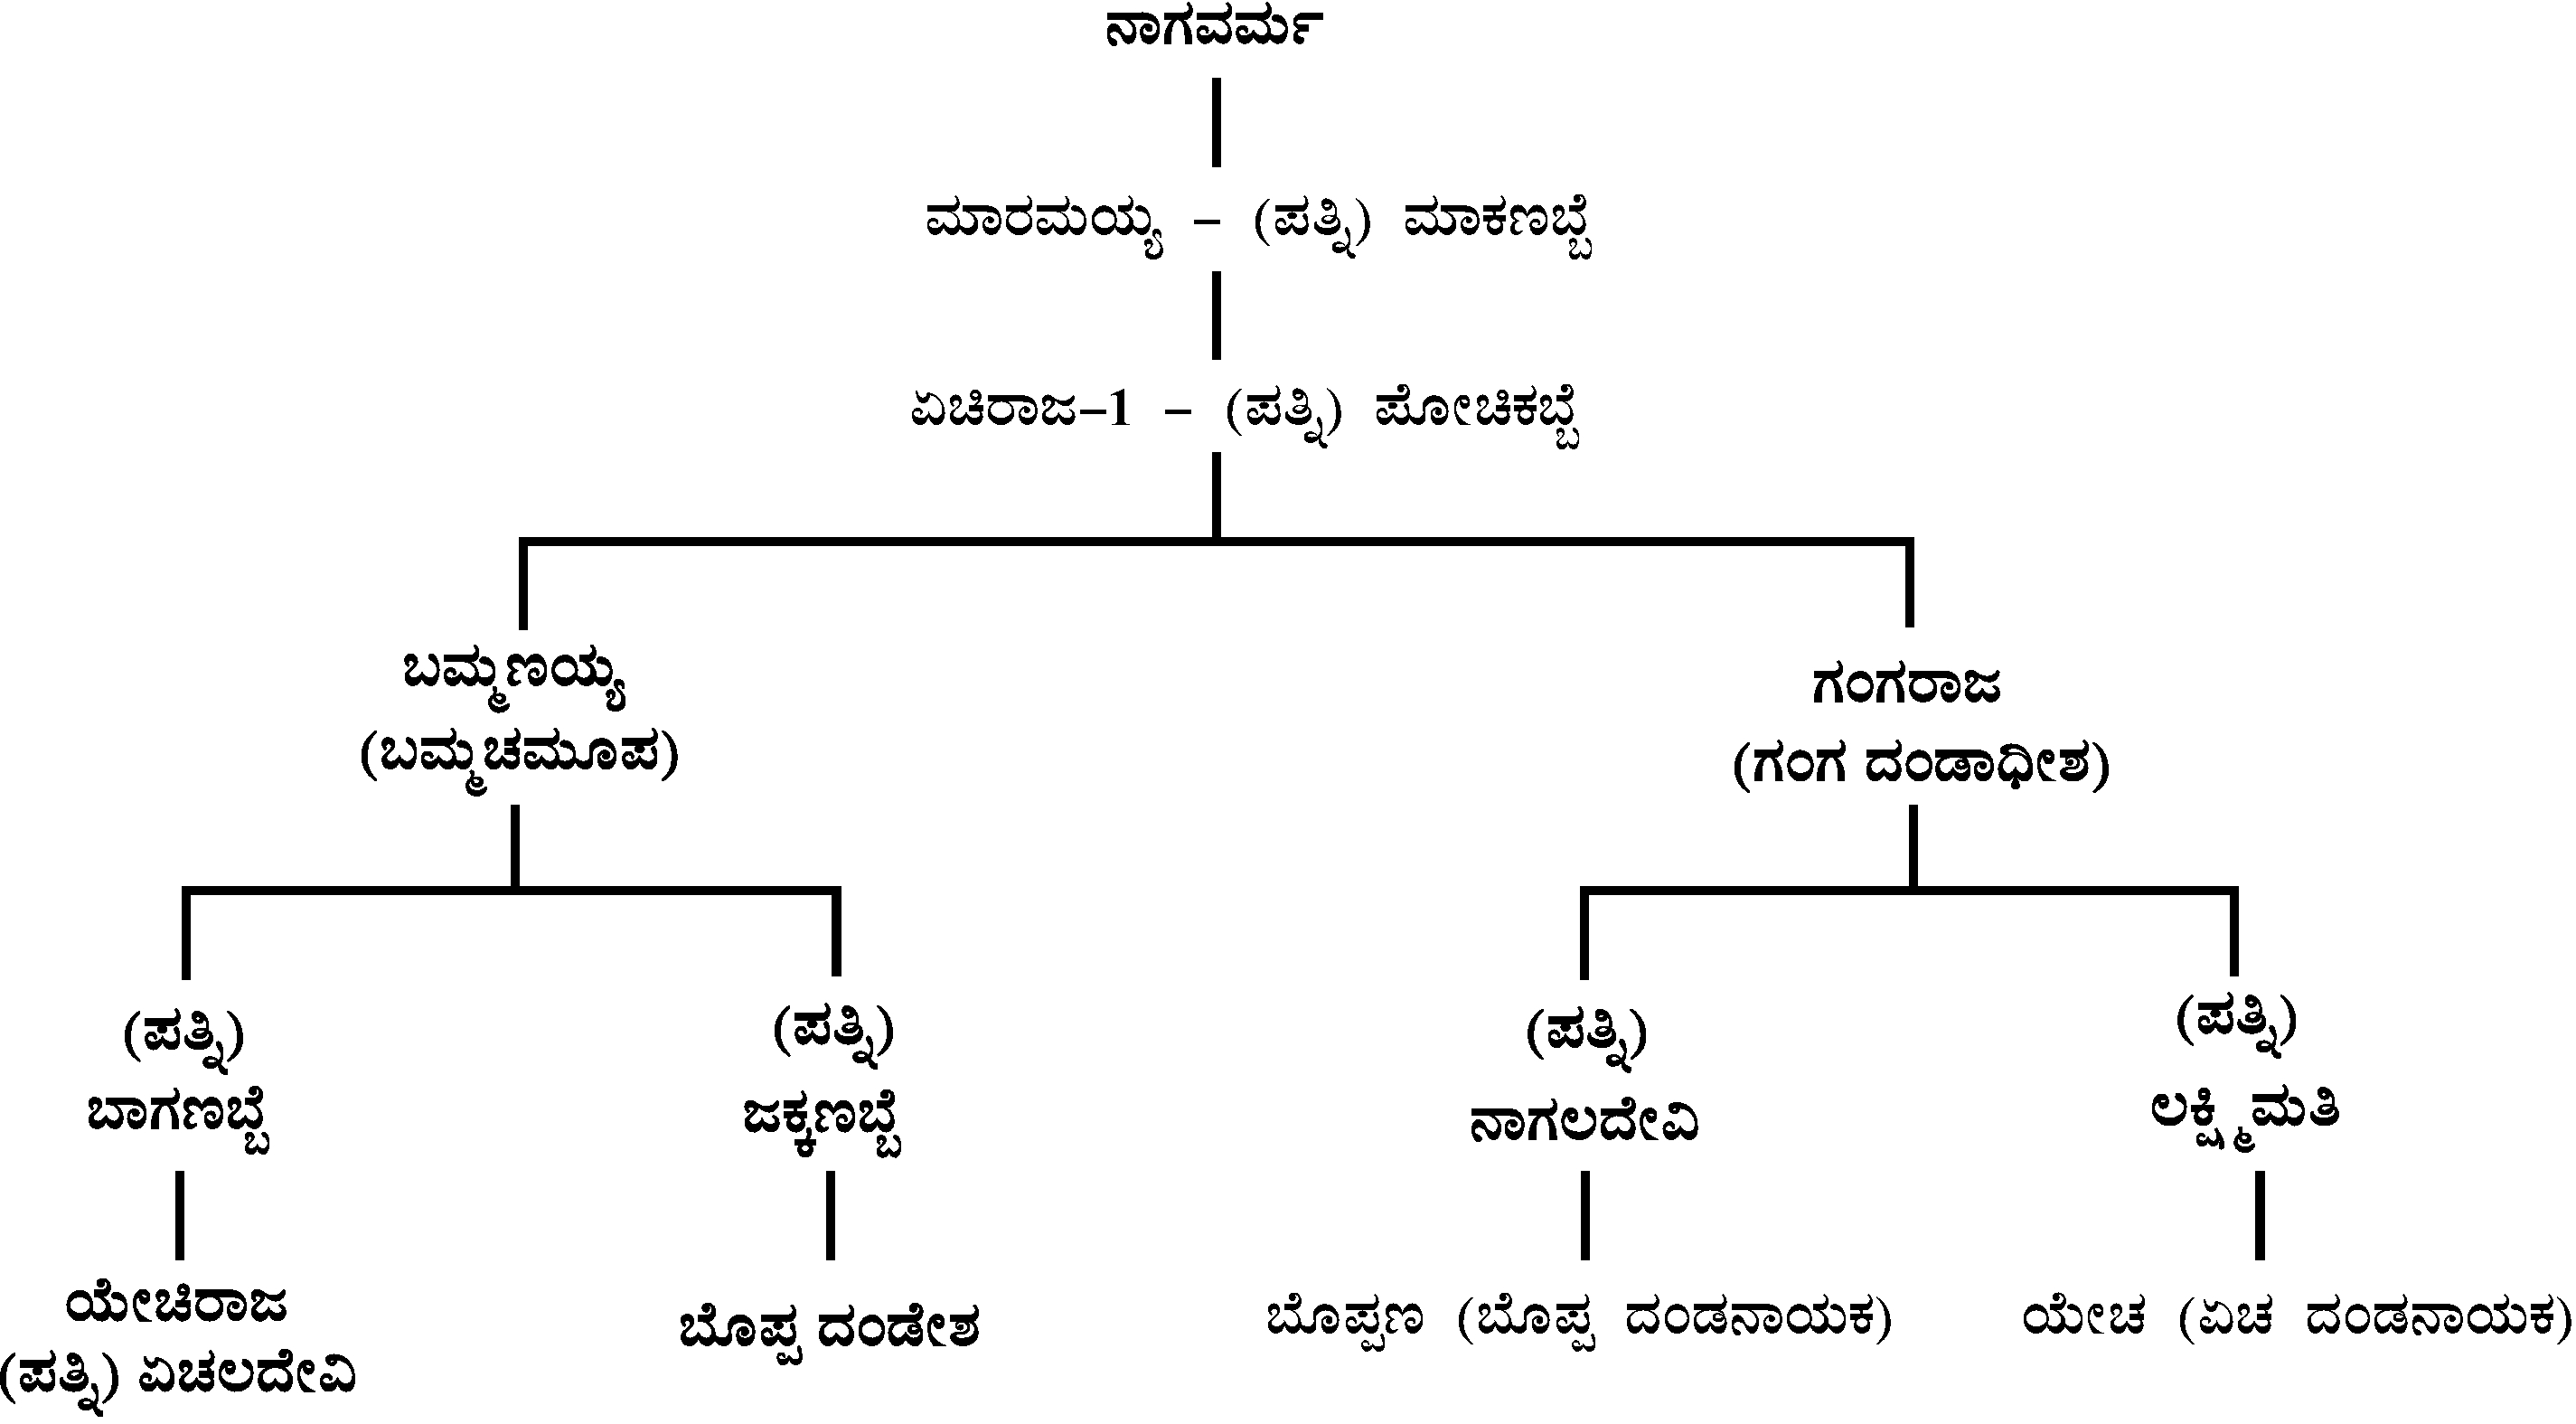
\includegraphics[scale=1.15]{images/chap3/chap3fig11.jpeg}
\end{figure}

ಮಹಾಪ್ರಧಾನ ಹಿರಿಯ ದಂಡನಾಯಕ ಗಂಗರಾಜನು ಮಹಾ ಸಾಮಂತಾಧಿಪತಿಯಾಗಿದ್ದನೆಂದು ತಿಳಿದುಬರುತ್ತದೆ.\endnote{ ಎಕ 7 ನಾಮಂ 32 ಕಂಬದಹಳ್ಳಿ 1118} ಇದೇ ಕಾಲದ ಗಂಗರಾಜನ ತಿಪ್ಪೂರು\index{ತಿಪ್ಪೂರು} ಶಾಸನದಲ್ಲಿ ಅವನನ್ನು ಸಾಮಂತಾಧಿಪತಿ ಎಂದು ಕರೆದಿಲ್ಲ. ಕ್ರಿ.ಶ.1115ರ ವೇಳೆಗೆ ಗಂಗರಾಜನು ಮಹಾಸಾಮಂತಾಧಿಪತಿ, ಮಹಾಪ್ರಚಂಡ ದಂಡನಾಯಕ ಹಾಗೂ ಮಹಾಪ್ರಧಾನ ದಂಡನಾಯಕನಾಗಿದ್ದ ವಿಚಾರ ಶ್ರವಣಬೆಳಗೊಳ ಶಾಸನದಿಂದ ತಿಳಿದುಬರುತ್ತದೆ.\endnote{ ಎಕ 2 ಶ್ರಬೆ 156 ಚಿಕ್ಕಬೆಟ್ಟ 1115 ಡಿಸೆಂಬರ್​ 2.} ಕ್ರಿ.ಶ.1120ರ ಶ್ರವಣಬೆಳಗೊಳದ ಇನ್ನೊಂದು ಶಾಸನದಲ್ಲೂ,\endnote{ ಎಕ 2 ಶ್ರಬೆ 136 ಚಿಕ್ಕಬೆಟ್ಟ 1120} ಕ್ರಿ.ಶ.1133ರ ಅಗ್ರಹಾರಬೆಳಗುಲಿ ಶಾಸನದಲ್ಲೂ ಕೂಡಾ, ಗಂಗರಾಜನ್ನು ಮಹಾಸಾಮಂತಾಧಿಪತಿ, ಮಹಾಪ್ರಚಂಡ\break ದಂಡನಾಯಕನೆಂದು ಹೇಳಿದೆ.\endnote{ ಎಕ 10 ಚರಾಪ ಅಗ್ರಹಾರ 98 ಬೆಳಗುಲಿ 1133}\textbf{ಆದಕಾರಣ ಮಹಾಪ್ರಧಾನ ಹುದ್ದೆಯಿಂದ ಮಹಾಸಾಮಂತ ಪದವಿಗೆ ಏರುತ್ತಿದ್ದರೆಂದು ಹೇಳಬಹುದು.}

\textbf{ಶ‍್ರೀಮನ್ಮಹಾಪ್ರಧಾನ\index{ಶ‍್ರೀಮನ್ಮಹಾಪ್ರಧಾನ} ಏಚಣ್ಣ ದಂಡನಾಯಕ\index{ಏಚಣ್ಣ ದಂಡನಾಯಕ}, ಬೋಕಣ್ಣ\index{ಬೋಕಣ್ಣ} ಮತ್ತು ವಿಷ್ಣು ದಂಡಾಧೀಶರು\index{ವಿಷ್ಣು ದಂಡಾಧೀಶ} (1138\general{\enginline{-}}1162):} ಕಲುಕಣಿ ಎಪ್ಪತ್ತಕ್ಕೆ\index{ಕಲುಕಣಿ (ಕಲಿಕಣಿ-ಕಲ್ಕಣಿ-ಕಲ್ಕುಣಿ-ಕಲುಕರೆ) ನಾಡು} ಶಿರೋಮಣಿಯಂತಿದ್ದ ನಾನಲಕೆರೆ(ಲಾಳನಕೆರೆ)ಯನ್ನು\index{ನಾನಲಕೆರೆ (ಲಾಳನಕೆರೆ)} ಗೌಡಿಕೆ ಉಂಬಳಿಯಾಗಿ\index{ಗೌಡಿಕೆ ಉಂಬಳಿ} ಪಡೆದು ಆಳುತ್ತಿದ್ದ ಏಚಿರಾಜನ ದಂಡನಾಯಕ ಹಾಗೂ ಅವನ ಮಕ್ಕಳು, ವಿಷ್ಣುವರ್ಧನನ ಮಂತ್ರಿಗಳೂ ದಂಡನಾಯಕರುಗಳೂ ಆಗಿದ್ದರು. ಮನುಮಾರ್ಗನು, ವಿಪ್ರಕುಲ ತಿಲಕನೂ \textbf{ವಸಿಷ್ಠಗೋತ್ರೋದ್ಭವನೂ} ಆಗಿದ್ದ ದ್ರೋಹಘರಟ್ಟನೆಂಬ ಬಿರುದನ್ನು ಹೊಂದಿದ್ದ ಶ‍್ರೀಮನ್ಮಹಾಪ್ರಧಾನ ದಂಡನಾಯಕ ಏಚಿರಾಜನು \textbf{“ವಿಷ್ಣುಭೂಪನ\index{ವಿಷ್ಣುಭೂಪ} ಸನುಮಂತ್ರಿಗಳೆನಿಸಿ ನೆಗಳ್ದರೊಳ್​ ಕರಮೆಸೆದಂ”. } ಅಂಡಲೆಯುತ್ತಿದ್ದ ಅರಿನೃಪರ ಹಿಂಡನ್ನು ಬೆಂಬೆತ್ತಿ ಹಿಡಿದು ತಂದು ಅವರನ್ನು ತನ್ನ ಒಡೆಯನ ಚರಣಗಳಿಗೆ ಆನತರಾಗುವಂತೆ ಮಾಡಿದ ಕೀರ್ತಿವಂತನೆಂದೂ, ವಿಷ್ಣುವಿಗೆ ಗರುಡನಂತೆ ತನ್ನ ಒಡೆಯನಿಗೆ ಆತ್ಮಭಕ್ತಿಯಿಂದ ಸೇವೆಸಲ್ಲಿಸಿ ಜಯವನ್ನು ಸಾಧಿಸಿಕೊಟ್ಟನೆಂದು ಧಾರಿಣಿಯು ಏಚಿರಾಜನನ್ನು ಹೊಗಳುತ್ತಿತ್ತೆಂದು ಶಾಸನವು ತಿಳಿಸುತ್ತದೆ.\endnote{ ಎಕ 7 ನಾಮಂ 61 ಲಾಳನಕೆರೆ 1138} ಇವರು ಕರ್ನಾಟಕ ಬ್ರಾಹ್ಮಣ ವಂಶಕ್ಕೆ\index{ಕರ್ನಾಟಕ ಬ್ರಾಹ್ಮಣ ವಂಶ} ಸೇರಿದವರು.(ಇಂದಿನ ಹೊಯ್ಸಳ ಕರ್ನಾಟಕ ಬ್ರಾಹ್ಮಣರು)

ಏಚಿರಾಜನ\index{ಏಚಿರಾಜ} ಪತ್ನಿ ಕಾಮಿಯಕ್ಕ\index{ಕಾಮಿಯಕ್ಕ}. ಇವನಿಗೆ ವಿಷ್ಣು ಮತ್ತು ಬೋಕಣ್ಣ ಎಂಬ ಇಬ್ಬರು ಮಕ್ಕಳು. ಆ ಕಾಲದಲ್ಲಿ ಅಧಿಕಾರಿಗಳು ತಮ್ಮ ಮಕ್ಕಳಿಗೆ ರಾಜನ ಹೆಸರನ್ನು ಇಡುತ್ತಿದ್ದುದು ರೂಢಿ, ಅದರಂತೆ ಏಚಿರಾಜನೂ ತನ್ನ ಮೊದಲ ಮಗನಿಗೆ ವಿಷ್ಣು ಅಥವಾ ಬಿಟ್ಟಿಯಣ್ಣ\index{ಬಿಟ್ಟಿಯಣ್ಣ} ಎಂದು ಹೆಸರಿಟ್ಟನು. ಮುಂದೆ ಇವನು ಬಿಟ್ಟಿದೇವ ದಂಡಾಧೀಶನೆಂದು ಹೆಸರುವಾಸಿಯಾದನು. \textbf{“ಬಿಟ್ಟಿದೇವ ದಂಡಾಧೀಶನು ನುಡಿದುದೇ ತಾಮ್ರಶಾಸನ, ಅವನು ಸಂಪಾದಿಸಿದ ಧನವೆಲ್ಲ ಸಜ್ಜನರಾದ ಪಂಡಿತರಿಗೆ”} ಎಂದು ಶಾಸನ ಹೊಗಳಿದೆ. ಮಂತ್ರಿಯಾಗಿದ್ದ ಬೋಕಣ್ಣನು \textbf{“ಬೀರಂ ಬಿಂಕಂ ಅದೇವುದೋ ಹಾರುವ ನಿನಗೆಂದು ಗಳಹನ ಬಾಯೊಳಕ್ಕೆ ಕೂರಲಗನ್ನು ಕುತ್ತುವ ವೀರಗ್ರಾ}ಣಿ”ಯಾಗಿದ್ದನಂತೆ.

ಇವರಿಗೆ ಬಿಟ್ಟೀದೇವ, ಬೋಕಣ್ಣರಲ್ಲದೆ, ಮಹದೇವ\index{ಮಹದೇವ}, ಹರಿಹರದೇವ\index{ಹರಿಹರದೇವ} ಮತ್ತು ಯೀಚಣ\index{ಯೀಚಣ} ಎಂಬ ಇನ್ನೂ ಮೂರು ಜನ ಮಕ್ಕಳಿದ್ದರು. ಮುಂದೆ ವಿಷ್ಣುದೇವ, ಬೋಕಂಣ ಮತ್ತು ಹರಿಹರದೇವ ಇವರು ದಂಡನಾಯಕರೂ ಮಂತ್ರಿಗಳೂ ಆದರು. ಉಳಿದವರ ಬಗ್ಗೆ ಹೆಚ್ಚಿನ ವಿವರಗಳು ತಿಳಿದುಬರುವುದಿಲ್ಲ. ಮಹಾಪ್ರಧಾನ ದಂಡನಾಯಕ, ಮಂತ್ರಿ ಪದವಿ ವಂಶಪಾರಂಪರ್ಯವಾಗಿದ್ದರೂ, ಅದಕ್ಕೆ ತಕ್ಕ ಅರ್ಹತೆಯೂ ಬೇಕು ಎಂಬುದು ಇದರಿಂದ ವ್ಯಕ್ತವಾಗುತ್ತದೆ.

ವಸುಂಧರೆಯನ್ನು ಗೆದ್ದು ಅದಕ್ಕೆ ತನ್ನ ಮುದ್ರಿಕೆಯನ್ನು ಒತ್ತಿ ತನ್ನ ಕೈಗಿತ್ತ ಏಚಿರಾಜನ ಪ್ರಸಿದ್ಧಿಗೆ ಮೆಚ್ಚಿ, ವಿಷ್ಣುವರ್ಧನನು\index{ವಿಷ್ಣುವರ್ಧನ (ದೇವರು) (ಹೊಯ್ಸಳರ ದೊರೆ)} ಅವನಿಗೆ ನಾನಲಕೆರೆಯನ್ನು ಗೌಡಿಕೆಯ ಉಂಬಳಿಯಾಗಿ ಧಾರೆ ಎರೆದು ಕೊಟ್ಟನು. ಅರಿಬಿರುದರದಂಡನಾಥ ಮತ್ತಮಾತಂಗ ಸಿಂಹನೆನಿಸಿದ್ದವನೂ, ಹೊಯ್ಸಳರಾಜ್ಯ ಸಮುದ್ಧರಣನೂ ಆಗಿದ್ದ ಏಚಿರಾಜನು ನಾನಲಕೆರೆಯ ಮೂಲ ಮಲ್ಲಿಕಾರ್ಜುನ ದೇವಾಲಯಕ್ಕೆ ಒಂದು ಸಾವಿರ ಅಡಿಕೆಮರದ ತೋಟವನ್ನು, ಗದ್ದೆ ಬೆದ್ದಲುಗಳನ್ನು ದತ್ತಿಯಾಗಿ ಬಿಟ್ಟನು. ಏಚಿರಾಜನ ಮಗ ಬಿಟ್ಟೀದೇವ ದಂಡಾಧೀಶನು ಯೆಳಂದೂರು ತಾಲ್ಲೂಕು ಅಗರ(ದುರ್ಗಅಗ್ರಹಾರ)\index{ಅಗರ(ದುರ್ಗಅಗ್ರಹಾರ)} ಗ್ರಾಮದ ಲಕ್ಷ್ಮೀನರಸಿಂಹ (ಹಿಂದಿನ ಸಿಂಗಪೆರುಮಾಳ್\index{ಸಿಂಗಪೆರುಮಾಳ್​}) ದೇವಾಲಯಕ್ಕೆ ದತ್ತಿಯನ್ನು ಬಿಟ್ಟಿರುವ ವಿಚಾರ ಅಲ್ಲಿರುವ ತ್ರುಟಿತ ಶಾಸನದಿಂದ ತಿಳಿದುಬರುತ್ತದೆ.\endnote{ ಎಕ 4 ಯಳಂ 84 ಮತ್ತು 85 ಅಗರ 12ನೇ ಶ.} ಬಹುಶಃ ಈ ದೇವಾಲಯವನ್ನು ವಿಷ್ಣುದಂಡಾಧೀಶನೇ ನಿರ್ಮಿಸಿರಬಹುದು.

ಒಂದನೆಯ ನರಸಿಂಹನ ಕಾಲದಲ್ಲೂ \textbf{ಬಿಟ್ಟಿಯಣ್ಣ ಅಥವಾ ವಿಷ್ಣು ದಂಡಾಧೀಶನು ಮಹಾಪ್ರಧಾನ ದಂಡನಾಯಕ\-ನಾಗಿದ್ದನು.} ಹುಣಸೂರು\index{ಹುಣಸೂರು} ತಾಲ್ಲೂಕು ಧರ್ಮಾಪುರ\index{ಧರ್ಮಾಪುರ} ಗ್ರಾಮದ ಚೆನ್ನಕೇಶವ ದೇವಾಲಯದಲ್ಲಿರುವ ಶಾಸನದಲ್ಲಿ, ಒಂದನೆಯ ನರಸಿಂಹನು ಆರಿದವಾಳಿಕೆಯ ತೊಗರವಾಡಿ, ಮನ್ನೆಯ ಬೂವನಹಳ್ಳಿಗಳ ಸಹಿತ ಧರ್ಮಾಪುರವೆಂಬ ಅಗ್ರಹಾರವನ್ನು ಮಾಡಿ, ಮಹಾಪ್ರಧಾನ ದಂಡನಾಯಕ ಬಿಟ್ಟಿಯಣ್ಣ, ಹಿರಿಯ ಭಂಡಾರಿ ಹುಳ್ಳಯ್ಯ\index{ಹಿರಿಯ ಭಂಡಾರಿ ಹುಳ್ಳಯ್ಯ}, ಪಸಾಯ್ತ ಸುರಿಗೆಯ ನಾಗಯ್ಯ\index{ಸುರಿಗೆಯ (ಸುರಗಿಯ) ನಾಗಯ್ಯ (ನಾಗಿದೇವ, ನಾಗಣ್ಣ)}, ಲಕುಮಯ್ಯಗಳ\index{ಲಕುಮಯ್ಯ} ಸಮಕ್ಷಮ ಅಲ್ಲಿಯ ಕೇಶವ ದೇವರ ಮೂಲಿಗ ಶ‍್ರೀಧರಯ್ಯನ\index{ಮೂಲಿಗ ಶ‍್ರೀಧರಯ್ಯ} ಕೈಯಲು ಸರ್ವನಮಸ್ಯವಾಗಿ ನೀಡಿದನೆಂದು ಹೇಳಿದೆ.\endnote{ ಎಕ 4 ಹುಣ 24 ಧರ್ಮಾಪುರ 1162} ವಿಷ್ಣುದಂಡಾಧೀಶ\-ನನ್ನು ಶಾಸನವು ಬಹಳವಾಗಿ ಸ್ತುತಿಸಿದ್ದು, ಈ ದೇವಾಲಯವನ್ನು ಮತ್ತು ಅಗ್ರಹಾರಗಳನ್ನು ಈತನೇ ನಿರ್ಮಿಸಿರುವ ಸಾಧ್ಯತೆ ಇದೆ

\begin{verse}
\textbf{ನೀಳಾಚಳಮಂ ಸಾಧಿಸಿ} \\\textbf{ಕಾಳನ ತಲೆಗೊಂಡನಿರದೆ ಕೊಂಗರ ಪಡೆಯಂ} \\\textbf{ಧೂಳೀಪಟಮಾಡಿ ಕಿಡಿಸಿದ} \\\textbf{ಕಾಳಾಂತಕನಲುತೆ ವಿಷ್ಣುದಂಡಾಧೀಶನುಂ}
\end{verse}

ವಿಷ್ಣುದಂಡಾಧೀಶನು ಕೊಂಗರನ್ನು ಸೋಲಿಸಿ, ಕಾಳರಾಜನನ್ನು ಕೊಂದು, ನೀಲಾಚಲ(ನೀಲಗಿರಿ)ಯನ್ನು ಗೆದ್ದು\-ಕೊಟ್ಟನೆಂದು ಇಲ್ಲಿ ಸ್ಪಷ್ಟವಾಗಿ ಹೇಳಿದೆ. “ವಿಜಯನಾರಸಿಂಹನು\index{ವಿಜಯನಾರಸಿಂಹ} ಸ್ವತಃ ಚೋಳರಾಜ್ಯಕ್ಕೆ ದಂಡೆತ್ತಿಹೋಗಿ ಚೋಳರನ್ನು ಪರಾಭವಗೊಳಿಸಿ, ಕೊಂಗು ಕಳಿಂಗ ರಾಜರನ್ನು ಸೋಲಿಸಿ ಅವರನ್ನು ಹೊಡೆದಟ್ಟಿದನು. ಈ ಕಾಲದಲ್ಲಿ ಕೆಲವು ಪ್ರಾಂತಗಳು ಪ್ರಕ್ಷುಬ್ದವಾಗಿ ಹೊಯಿಸಳ ಸಾಮ್ರಾಜ್ಯದಿಂದ ಸಿಡಿದೇಳಲು ಹವಣಿಸಿದಾಗ ವಿಜಯನಾರಸಿಂಹನ ಅಮಾತ್ಯ ಬಿಟ್ಟಿಗನು(ವಿಷ್ಣ) ಆ ಕ್ಷೋಭೆಯನ್ನು ನಿಗ್ರಹಿಸಿದನು. ಈ ಬಿಟ್ಟಿಯು ವಿಷ್ಣವರ್ಧನನ ಕಾಲದಲ್ಲಿ ಸಾಮಂತನಾಗಿದ್ದು ನೀಲಾಚಲವನ್ನು ವಶಪಡಿಸಿಕೊಂಡು ಕಾಲರಾಜ ಶಿರಚ್ಛೇದ ಮಾಡಿ ಕೊಂಗಸೇನೆಯನ್ನು ಚೂರ್ಣೀಕರಿಸಿದ ವೀರ. ದಂಡನಾಯಕರಾದ ಮರಿಯಾನೆಯೂ\index{ಮರಿಯಾನೆ (ದಂಡನಾಯಕ)} ಭರತನೂ\index{ಭರತ (ಭರತಿಮಯ್ಯ) ದಂಡನಾಯಕ}\break ವಿಜಯನಾರಸಿಂಹನ ಕಾಲದಲ್ಲಿ ದಂಡನಾಯಕರಾಗಿದ್ದರು ಎಂದು ವಿದ್ವಾಂಸರು ಹೇಳಿದ್ದಾರೆ”.\endnote{ ಕೃಷ್ಣರಾವ್​ ಪ್ರೊ॥ ಎಂ.ವಿ., ಕರ್ನಾಟಕದ ಇತಿಹಾಸ ದರ್ಶನ, ಪುಟ 257} ಈ ಸಾಧನೆಗಳನ್ನು ಮಾಡಿದವನು ವಿಷ್ಣುದಂಡಾಧೀಶ ಅಥವಾ ಬಿಟ್ಟಿಯಣ್ಣನೆಂದೂ, ಅವನ ಜೊತೆಗೆ ಭಂಡಾರಿ ಹುಳ್ಳ, ಸುರಿಗೆಯ ನಾಗಯ್ಯ, ಲಕುಮಯ್ಯರು ಇದ್ದರೆಂದು, ಅರಸನಾದ ನರಸಿಂಹನೂ ಕೂಡಾ ಅವರ ಜೊತೆ ಇದ್ದನೆಂದು ಧರ್ಮಾಪುರ\index{ಧರ್ಮಾಪುರ} ಶಾಸನದಿಂದ ತಿಳಿದು ಬರುತ್ತದೆ.ಲಾಳನಕೆರೆಯ ಇನ್ನೊಂದು ಶಾಸನದಲ್ಲಿ ದಂಡಾಧೀಶ ಬೋಕಣ ಮತ್ತು ದಂಡನಾಯಕ ಹರಿಯಣ್ಣನ ಪ್ರಸ್ತಾಪ\-ವಿದೆ.\endnote{ ಎಕ 7 ನಾಮಂ 63ಲಾಳನಕೆರೆ 1165} ಈ ಶಾಸನದ ಕಾಲಕ್ಕೆ ಬೋಕಂಣನು\index{ಬೋಕಂಣ} ಮಂತ್ರಿ ಪದವಿಯ ಜೊತೆಗೆ ದಂಡಾಧೀಶನ ಪದವಿಯನ್ನು ಪಡೆದಿದ್ದನು. ಹರಿಹರ ದೇವನು ದಂಡನಾಯಕ ಪದವಿಯನ್ನು ಪಡೆದು, ದಂಡನಾಯಕ ಹರಿಯಂಣನೆನಿಸಿದನು. ಏಚಣ್ಣನ ವಂಶಾವಳಿ ಈ ಕೆಳಗಿನಂತಿದೆ.

\begin{figure}[H]
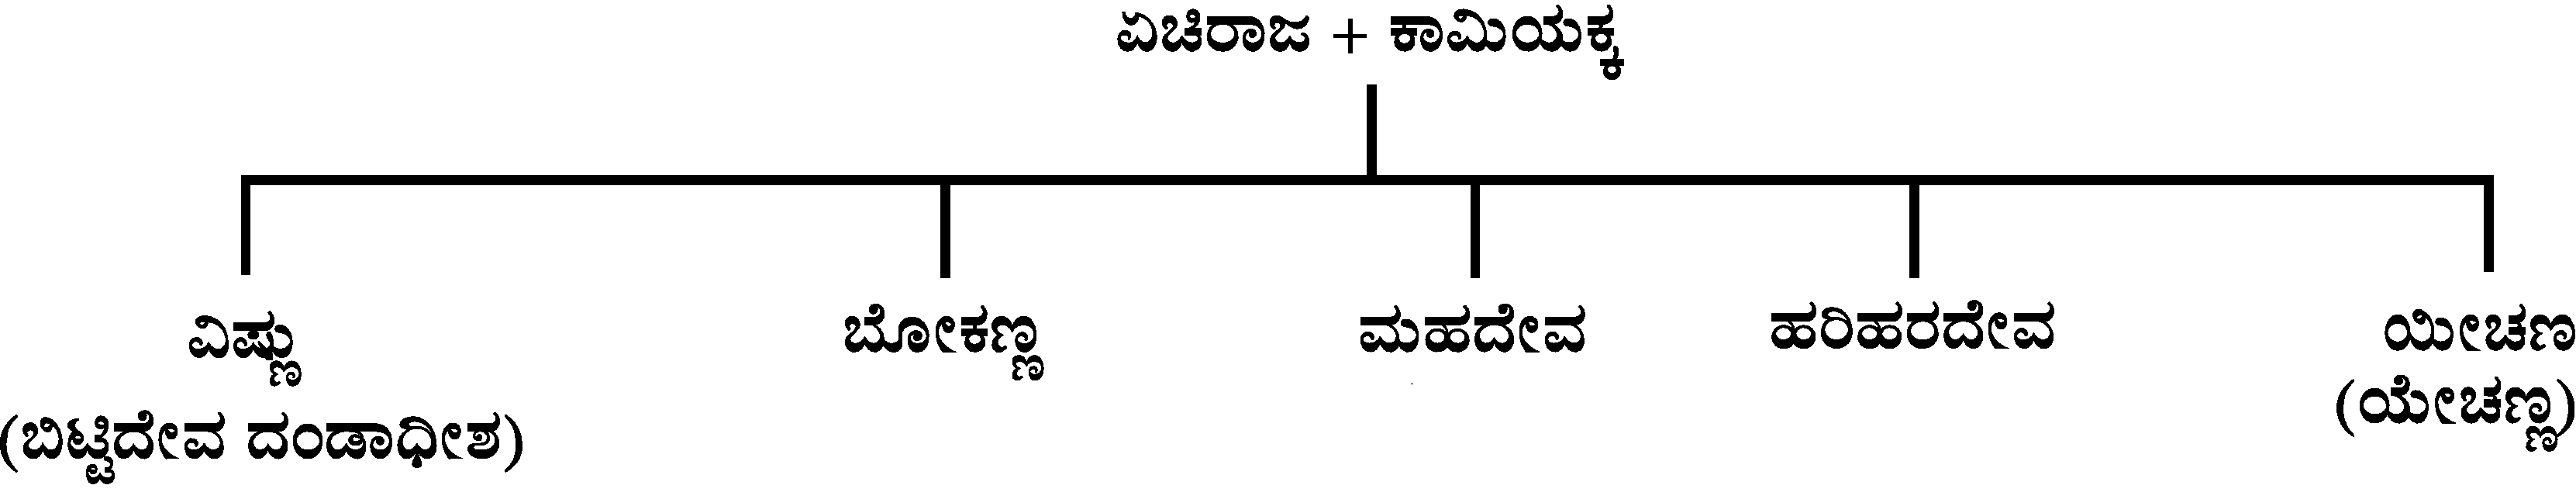
\includegraphics[scale=1.15]{images/chap3/chap3fig12.jpeg}
\end{figure}

\textbf{ಮಹಾಪ್ರಧಾನ\index{ಮಹಾಪ್ರಧಾನ} ಮರಿಯಾನೆ ದಂಡನಾಯಕ\index{ಮರಿಯಾನೆ (ದಂಡನಾಯಕ)} ಮತ್ತು ಭರತ ದಂಡನಾಯಕ\index{ಭರತ (ಭರತಿಮಯ್ಯ) ದಂಡನಾಯಕ} (1142- 1183):} ಹೊಯ್ಸಳರ ಕಾಲದ ಪ್ರಖ್ಯಾತ ದಂಡನಾಯಕರಾಗಿದ್ದ ಮರಿಯಾನೆ ದಂಡನಾಯಕರ ವಂಶದ ವಿವರಗಳನ್ನು ಇತಿಹಾಸ ಪ್ರಸಿದ್ಧ ಅಳಿಸಂದ್ರ ಶಾಸನವು ನೀಡುತ್ತದೆ.\endnote{ ಎಕ 7 ನಾಮಂ 72 ಅಳಿಸಂದ್ರ 1048, 1103, 1182, 1183} ಇದೊಂದು ಸಂಕೀರ್ಣ ಶಾಸನವಾಗಿದ್ದು ಇದರಲ್ಲಿ ಮೂರು\enginline{-}ನಾಲ್ಕು ತಲೆಮಾರಿನ ವಿವರಗಳಿದ್ದು, ನಾಲ್ಕು ತೇದಿಗಳಿವೆ. ಅಳಿಸಂದ್ರ ಶಾಸನದಲ್ಲಿ ನೀಡಿರುವ ದಂಡನಾಯಕರ ವಂಶವೃಕ್ಷವನ್ನು ಎಪಿಗ್ರಾಫಿಯಾ ಸಂಪಾದಕರು ನೀಡಿದ್ದಾರೆ.\endnote{ ಎಪಿಗ್ರಾಫಿಯಾ ಕರ್ನಾಟಿಕಾ, ಸಂಪುಟ 7, ಪೀಠಿಕೆ ಪುಟ lviii} ಈ ವಂಶದ ಮಹಾಪ್ರಧಾನ ದಂಡನಾಯಕರನ್ನು ಮತ್ತು ದಂಡನಾಯಕರುಗಳನ್ನು ಬೇರೆಬೇರೆಯಾಗಿ ಅಧ್ಯಯನ ಮಾಡಲಾಗಿದೆ.

ವಿನಯಾದಿತ್ಯನ\index{ವಿನಯಾದಿತ್ಯ} ರಾಣಿ ಕೆಳೆಯಬ್ಬರಸಿಯು\index{ಕೆಳೆಯಬ್ಬರಸಿ}, ಮರಿಯಾನೆ ದಂಡನಾಯಕನನ್ನು ತನ್ನ ತಮ್ಮನಂತೆ ರಕ್ಷಿಸಿ,\break ದೇಕವ್ವೆ ದಂಡನಾಯಕಿತಿಯ ಜೊತೆ ಮದುವೆಯನ್ನು ಮಾಡಿಸಿ ಶಕ 967 ಅಂದರೆ ಕ್ರಿ.ಶ.1048 ರಲ್ಲಿ ಆಸಂದಿನಾಡ ಸಿಂಧಗೆರೆಯ ಪ್ರಭುತ್ವವನ್ನು ನೀಡುತ್ತಾಳೆ. ಇವನೇ \textbf{ಹಿರಿಯ ಮರಿಯಾನೆ ದಂಡನಾಯಕ\index{ಹಿರಿಯ ಮರಿಯಾನೆ ದಂಡನಾಯಕ}. }ಈ ಹಿರಿಯ ಮರಿಯಾನೆ ದಂಡನಾಯಕ ಮತ್ತು ಚಾಮವ್ವೆ ದಂಡನಾಯಕಿತ್ತಿಗೆ\index{ಚಾಮವ್ವೆ ದಂಡನಾಯಕಿತ್ತಿ} ಜನಿಸಿದ, ಪದುಮಲದೇವಿ\index{ಪದುಮಲದೇವಿ}, ಚಾಮಲದೇವಿ\index{ಚಾಮಲದೇವಿ} ಮತ್ತು ಬೊಪ್ಪಾದೇವಿಯರನ್ನು\index{ಬೊಪ್ಪಾ ದೇವಿ} ಒಂದೇ ಹಸೆಮಣೆಯಲ್ಲಿ, ಬಲ್ಲಾಳ ದೇವನು ವಿವಾಹಮಾಡಿಕೊಟ್ಟು, ತಾಯ ಮೊಲೆವಾಲ ಋಣಕ್ಕೆ ಮರಿಯಾನೆ ದಂಡನಾಯಕನಿಗೆ ಶಕ 1025 ಅಂದರೆ ಕ್ರಿ.ಶ.1103 ರಲ್ಲಿ, ಎರಡನೆಯ ಪರ್ಯಾಯದಲು ಪ್ರಭುತ್ವಸಹಿತವಾಗಿ ಸಿಂಧಗೆರೆಯನ್ನು\index{ಸಿಂಧಗೆರೆ} ಪುನರ್​ ಧಾರಾಪೂರ್ವಕವಾಗಿ ಬಿಡುತ್ತಾನೆ.

ಹಿರಿಯ ಮರಿಯಾನೆ ದಂಡನಾಯಕನ ಮಯ್ದುನ ಗಂಗರಾಜ\index{ಗಂಗರಾಜ} ಅಥವಾ ಗಂಗಣ್ಣ ದಂಡಾಧೀಶ. ಇವನ ಮಗ ಏಚಿರಾಜ ಅಥವಾ ಬೊಪ್ಪದಂಡಾಧೀಶ\index{ಬೊಪ್ಪ ಚಮೂಪ (ದಂಡನಾಯಕ - ದಂಡಾಧೀಶ)}. ಈ ಬೊಪ್ಪ ದಂಡಾಧೀಶನ ಮೈದುನರಾದ ಮರಿಯಾನೆ(ಕಿರಿಯ)\index{ಮರಿಯಾನೆ(ಕಿರಿಯ)} ದಂಡನಾಯಕ ಮತ್ತು ಭರತೇಶ್ವರ\index{ಭರತೇಶ್ವರ} ದಂಡನಾಯಕರು ವಿಷ್ಣುವರ್ಧನನ ಬಳಿ ಶ್ರಿಮನ್ಮಹಾಪ್ರಧಾನ ದಂಡನಾಯಕರಾಗಿದ್ದರು. ಇವರು ಭೀಮಾರ್ಜುನರು ಮತ್ತು ಲವಕುಶರಂತೆ ಇದ್ದರೆಂದು ದಡಗ ಶಾಸನ ಹೇಳಿದೆ.\endnote{ ಎಕ 7 ನಾಮಂ 68 ದಡಗ 12ನೇ ಶ.} ಇದೇ ವರ್ಣನೆಯು ತಗಡೂರು\index{ತಗಡೂರು} ಶಾಸನದಲ್ಲೂ ಬಂದಿದೆ.\endnote{ ಎಕ 10 ಚರಾಪ 52 ತಗಡೂರು 12ನೇ ಶ} ಮರಿಯಾನೆ ದಂಡನಾಯಕನನ್ನು ವಿಷ್ಣುವರ್ಧನನು ತನ್ನ ಪಟ್ಟದಾನೆಯಂತೆ ನೆಚ್ಚಿಕೊಂಡಿದ್ದನು. ಪ್ರಭುಪೆರ್ಗ್ಗಡೆ ಯೇಚಿರಾಜ ಮತ್ತು ನಾಗಲದೇವಿ\index{ನಾಗಲದೇವಿ} ಇವರ ಮಗಳು ಜಕ್ಕಲದೇವಿ\index{ಜಕ್ಕಲದೇವಿ} ಈ ಎರಡನೇ ಮರಿಯಾನೆ ದಂಡನಾಯಕನ ಹೆಂಡತಿ.

ಭರತ ದಂಡಾಧೀಶನು \textbf{“ವಿಷ್ಣುಭೂಪನ ರಾಜ್ಯಸ್ಥಳಕ್ಕೆ ಮಿಸುಪೆಸೆವ ಹೇಮದ ಕಳಸ”}ದಂತಿದ್ದನು. ಮಾರಯ್ಯನ\index{ಮಾರಯ್ಯ} ಮಗಳು ಹರಿಯಲೆ\index{ಹರಿಯಲೆ} ಅಥವಾ ಚಿಕ್ಕಹರಿಯಲೆ\index{ಚಿಕ್ಕಹರಿಯಲೆ} ಭರತೇಶದಂಡನಾಯಕನ ಪತ್ನಿ. ಇಲ್ಲಿಂದ ಮುಂದೆ ಈ ವಂಶದೊಡನೆ ಸಂಬಂಧ ಹೊಂದಿದ್ದ ಬೇರೆ ದಂಡನಾಯಕರುಗಳ ವಂಶದ ವಿವರವಿದೆ. ಇವರಿಬ್ಬರೂ ವಿಷ್ಣುವರ್ಧನನ ಬಳಿ ಸರ್ವಾಧಿಕಾರಿಗಳೂ, ಮಾಣಿಕ ಭಂಡಾರಿಗಳು ಮತ್ತು ಪ್ರಾಣಾಧಿಕಾರಿಗಳೂ ಆಗಿದ್ದರು. ಭರತದಂಡನಾಯಕನು ತನ್ನ ಮಗನಿಗೆ ಬಿಟ್ಟಿದೇವನೆಂದು ಹೆಸರಿಟ್ಟು, ವಿಷ್ಣುವರ್ಧನನಿಗೆ ಒಂದುಸಾವಿರ ಹೊನ್ನು ಪಾದಪೂಜೆಯನ್ನು ಕೊಟ್ಟು ಆಸಂದಿನಾಡ ಸಿಂಧಗೆರೆಯನ್ನು, ಬಾಯ್​ಬೆಣ್ಣೆಗೆ ಬಗ್ಗವಳ್ಳಿಯನ್ನು, ಕಲಿಕಣಿನಾಡ ದಿಂಡಿಗನಕೆರೆಯ (ದಡಿಗನಕೆರೆ) (ಇಂದಿನ ದಡಗ) ಪ್ರಭುತ್ವವನ್ನು ಅವನ ಸ್ವಹಸ್ತದಿಂದ ಪಡೆದರು.

ವಿಷ್ಣುವರ್ಧನನ ಕಾಲದಲ್ಲಿ \textbf{ಶ‍್ರೀಮನ್ಮಹಾಪ್ರಧಾನ ದಂಡನಾಯಕ ಮರಿಯಾನೆ\index{ಮರಿಯಾನೆ (ದಂಡನಾಯಕ)} ಮತ್ತು ಶ‍್ರೀಮನ್ಮಹಾಪ್ರಧಾನ ದಂಡನಾಯಕ ಭರತಿಮಯ್ಯರು\index{ಭರತ (ಭರತಿಮಯ್ಯ) ದಂಡನಾಯಕ} ದಡಿಗನಕೆರೆಯ\index{ದಡಗ (ದಡಿಗ, ದಡಿಗನಕೆರೆ)}} (ಇಂದಿನ ದಡಗ\index{ದಡಗ (ದಡಿಗ, ದಡಿಗನಕೆರೆ)}) ಪಂಚಬಸದಿಯೊಳಗೆ ಬಾಹುಬಲಿ ಕೂಟವನ್ನು ಮಾಡಿಸಿ ಅದಕ್ಕೆ\break ಮರಿಯಾನೆಸಮುದ್ರದ\index{ಮರಿಯಾನೆ ಸಮುದ್ರ} ಬಯಲಲ್ಲಿ ಗದ್ದೆಬೆದ್ದಲು ತೋಟಗಳನ್ನು ದತ್ತಿಯಾಗಿ ಬಿಟ್ಟರು.\endnote{ ಎಕ 7 ನಾಮಂ 68 ದಡಗ 12ನೇ ಶ.} ಒಂದನೆಯ ನರಸಿಂಹನ ಕಾಲದಲ್ಲಿ ಕೂಡಾ ಇವರು ಮಹಾಪ್ರಧಾನರಾಗಿ ಮುಂದುವರೆದರು. ತಮ್ಮ ವಂಶಕ್ಕೆ ಸೇರಿದ ಸಿಂದಗೆರೆ\index{ಸಿಂದಗೆರೆ}, ಬಗ್ಗವಳ್ಳಿ\index{ಬಗ್ಗವಳ್ಳಿ} ಮತ್ತು ದಡಿಗನಕೆರೆಯ\index{ದಡಗ (ದಡಿಗ, ದಡಿಗನಕೆರೆ)} ಪ್ರಭುತ್ವವನ್ನು ನಾರಸಿಂಹನಿಗೆ 500 ಹೊನ್ನು ಪಾದಪೂಜೆಯನ್ನು ಕೊಟ್ಟು ಅವನ ಹಸ್ತದಿಂದ ಪುನರ್​ದತ್ತಿಯಾಗಿ ಪಡೆದರು.\endnote{ ಎಕ 7 ನಾಮಂ 72 ಅಳಿಸಂದ್ರ}

ಒಂದನೆಯ ನರಸಿಂಹನು ಈ ಹಿಂದೆ ತನ್ನ ಹಿರಿಯದೇವನು ಅಂದರೆ ವಿಷ್ಣುವರ್ಧನನು, ಕಂಬದಹಳ್ಳಿಯ\index{ಕಂಬದಹಳ್ಳಿ} ದೇವತಾ\-ಪೂಜೆಗೆ ಮತ್ತು ಮೊದಲಿಯಳ್ಳಿಯ\index{ಮೊದಲಿಯಳ್ಳಿ (ಹಳ್ಳಿ)} ಶಾಂತಿನಾಥದೇವರ ಪೂಜೆಗೆ ಬಿಟ್ಟಿದ್ದ ದತ್ತಿಗಳನ್ನು, ಗಂಡವಿಮುಕ್ತ ಸಿದ್ಧಾಂತದೇವರ\index{ಗಂಡವಿಮುಕ್ತ ಸಿದ್ಧಾಂತದೇವರು} ಗುಡ್ಡುಗಳಾದ ಮರಿಯಾನೆ ದಂಡನಾಯಕ ಮತ್ತು ಭರತಿಮಯ್ಯ ದಂಡನಾಯಕರ ವಿನಂತಿಯಮೇರೆಗೆ ಪುನಃ ದತ್ತಿಯಾಗಿ ಬಿಟ್ಟನು.\endnote{ ಎಕ 7 ನಾಮಂ 30 ಕಂಬದಹಳ್ಳಿ 12ನೇ ಶ.} ಇದೇ ಭರತಿಮಯ್ಯ ದಂಡನಾಯಕನು, ಕೇಸಿಮಯ್ಯ\index{ಕೇಸಿಮಯ್ಯ} ಮತ್ತು ಉದಯಮಯ್ಯ\index{ಉದಯಮಯ್ಯ} ಇವರೊಡಗೂಡಿ ಧರ್ಮಕ್ಕೆ ಸಹಾಯಕರಾಗಿ ಹಳೇಬೀಡು ಮಲ್ಲಿಕಾರ್ಜುನದೇವರಿಗೆ ದತ್ತಿಯನ್ನು ಬಿಟ್ಟನು.\endnote{ ಎಕ 9 ಬೇಲೂರು 342 ಹಳೇಬೀಡು 1142} ಹುಳ್ಳಚಮೂಪನು ಶ್ರವಣಬೆಳಗೊಳದಲ್ಲಿ ದೇವಕೀರ್ತಿ ಪಂಡಿತರ ನಿಶಿದಿಗೆಯನ್ನು ಮಾಡಿಸಿದಾಗ, ಅಲ್ಲಿ ಅವರ ಗುಡ್ಡುಗಳಾದ ಮಾಣಿಕ್ಯ ಭಂಡಾರಿ ಮರಿಯಾನೆ ದಂಡನಾಯ\-ಕರು, ಶ‍್ರೀಮನ್​ ಮಹಾಪ್ರಧಾನ ಸರ್ವಾಧಿಕಾರಿ ಪಿರಿಯ ದಂಡನಾಯಕ ಭರತಿಮಯ್ಯಗಳು ಇದ್ದಂತೆ ಹೇಳಿದೆ.\endnote{ ಎಕ 2 ಶ್ರಬೆ 71 ಚಿಕ್ಕಬೆಟ್ಟ 1163}

ದೊಡ್ಡಬೆಟ್ಟದ ಅಖಂಡಬಾಗಿಲಿನ ಎಡಬಲದಲ್ಲಿರುವ ಭುಜಬಲಿ ಮತ್ತು ಭರತೇಶ್ವರ ಸ್ವಾಮಿಯರ ಪ್ರತಿಮೆಗಳನ್ನು ಗಂಡವಿಮುಕ್ತ ಸಿದ್ಧಾಂತ ದೇವರ ಶಿಷ್ಯ ಭರತೇಶ್ವರ\index{ಭರತೇಶ್ವರ} ದಂಡನಾಯಕನು ಮಾಡಿಸಿದನು. ಅಖಂಡ ಬಾಗಿಲಿನ ಬಲಭಾಗದಲ್ಲಿರುವ ಭರತ ಬಾಹುಬಲಿ ಮತ್ತು ಕೇವಲಿಗಳ ಪ್ರತಿಮೆಗಳನ್ನು ದ್ವಾರಪಕ್ಷದ ಶೋಭಾರ್ಥವಾಗಿಯೂ, ಮಹಾಸೋಪಾನವನ್ನು, ರಂಗದ ಹಪ್ಪಳಿಗೆಯನ್ನು, ಗೊಮ್ಮಟದೇವರ ಸುತ್ತಲೂ ಇರುವ ಹಪ್ಪಳಿಗೆಯನ್ನು ಮರಿಯಾನೆ ದಂಡನಾಥನ\index{ಮರಿಯಾನೆ (ದಂಡನಾಯಕ)} ಅನುಜ ಭರತಮಯ್ಯ ದಂಡನಾಯಕನು ಮಾಡಿಸಿದನು. ಭರತ ಚಮೂಪತಿಯ ಸುತೆ ಶಾಂತಲದೇವಿ\index{ಶಾಂತಲೆ (ಶಾಂತಲದೇವಿ)} ಅವಳ ಗಂಡ ಬೂಚಿರಾಜ\index{ಬೂಚಿರಾಜ} ಹಾಗೂ ಇವರ ಮಗ ಮರಿಯಾನೆ (ಮೂರನೆಯ)\index{ಮರಿಯಾನೆ (ದಂಡನಾಯಕ)} ಈ ಶಾಸನವನ್ನು ಬರೆಸಿದರು.\endnote{ ಎಕ 2 ಶ್ರಬೆ 371, 372, 373 ದೊಡ್ಡಬೆಟ್ಟ ( ಅಖಂಡಬಾಗಿಲ ಎಡಬಲದಲ್ಲಿ) 12ನೇ ಶ.} ಇವರು ಡಾಕರಸ ದಂಡನಾಯಕನ\index{ಡಾಕರಸ ದಂಡನಾಯಕ} ವಂಶದವರು ಎಂಬುದನ್ನು ಅಳಿಸಂದ್ರ ಶಾಸನ ಹೇಳಿದ್ದು ಮರಿಯಾನೆ ಮತ್ತು ಭರತರನ್ನು ಮಾತ್ರ ಶ‍್ರೀಮನ್​ ಮಹಾಪ್ರಧಾನ ದಂಡನಾಯಕರು, ಸರ್ವಾಧಿಕಾರಿಗಳು, ಮಾಣಿಕಭಂಡಾರಿಗಳು ಮತ್ತು ಪ್ರಾಣಾಧಿಕಾರಿಗಳೂ ಆಗಿದ್ದರೆಂದು ಹೇಳುತ್ತದೆ. ಆದುದರಿಂದ\break ಮಹಾಪ್ರಧಾನ ಎಂಬುದು ಕೇವಲ ಗೌರವಸೂಚಕ ಪದ ಅಥವಾ ಹುದ್ದೆಯಲ್ಲ. ಅದೊಂದು ಉನ್ನತದರ್ಜೆಯ ಅಧಿಕಾರ ಪದವಿಯಾಗಿತ್ತು ಎಂಬುದು ತಿಳಿದುಬರುತ್ತದೆ.

ಭರತನ ಮಗಳು ಬಮ್ಮಲೆಯ ಕರಗುಂದ ಶಾಸನದಲ್ಲಿ ಮರಿಯಾನೆಯನ್ನು ಬಮ್ಮಲೆಯ\index{ಬಮ್ಮಲೆ} ಕಿರಿಯಯ್ಯ ಎಂದು ಹೇಳಿರುವುದರಿಂದ, ಡಾಕರಸ ದುಗ್ಗವ್ವೆಯರಿಗೆ ಭರತನೇ ಮೊದಲನೆಯ ಮಗ ಮರಿಯಾನೆಯೇ ಎರಡನೆಯ ಮಗನಾಗುತ್ತಾನೆ. ಚಿಕ್ಕಮಗಳೂರು ತಾಲ್ಲೂಕು ಸಿಂಧಗಿರಿ(ಸಿಂಧಗೆರೆ) ಶಾಸನವು, ಅಳೀಸಂದ್ರದ ಶಾಸನದಲ್ಲಿ ಹೇಳಿರುವ ಕೆಲವು ವಿವರಗಳನ್ನು ನೀಡುತ್ತದೆ. \textbf{“ವೀರ ವಿಷ್ಣುವರ್ಧನ ದೇವನಣುಗಿನರ್ಕ್ಕರಿನ ದಂಡನಾಯಕ ಅನ್ವಯಾಗತ ಮಹಾಪ್ರಧಾನಿ\index{ಅನ್ವಯಾಗತ ಮಹಾಪ್ರಧಾನ} ಭರತ ದಂಡನಾಯಕ ಮತ್ತು ಮರಿಯಾನೆ ದಂಡನಾಯಕ”} ಎಂದು ಹೇಳಿದ್ದು ಇವರ ವಂಶವೃಕ್ಷವನ್ನು ನೀಡಿದೆ.\endnote{ ಎಕ 11 ಚಿಕ್ಕಮಗಳೂರು 210 ಸಿಂಧಗಿರಿ 1103

ಎಕ 11 ಚಿಕ್ಕಮಗಳೂರು 211 ಸಿಂಧಗಿರಿ 1137} ಭರತ ಮತ್ತು ಮರಿಯಾನೆ ಇವರು ದಂಡನಾಯಕರ ಪದವಿಯಿಂದ, ಹಿರಿಯ ದಂಡನಾಯಕ ಮತ್ತು ಅನ್ವಯಾಗತ ಮಹಾಪ್ರಧಾನಿಗಳ ಪಟ್ಟಕ್ಕೇರಿದರು ಎಂಬುದು ಇದರಿಂದ ತಿಳಿದುಬರುತ್ತದೆ. ಅಳಿಸಂದ್ರ ಹಾಗೂ ಮೇಲೆ ಉಲ್ಲೇಖಿಸಿದ ಇತರ ಶಾಸನಗಳಿಂದ ಇವರ ವಂಶಾವಳಿಯನ್ನು ಈ ಕೆಳಕಂಡ ರೀತಿ ನೀಡಬಹುದು.

\begin{figure}[H]
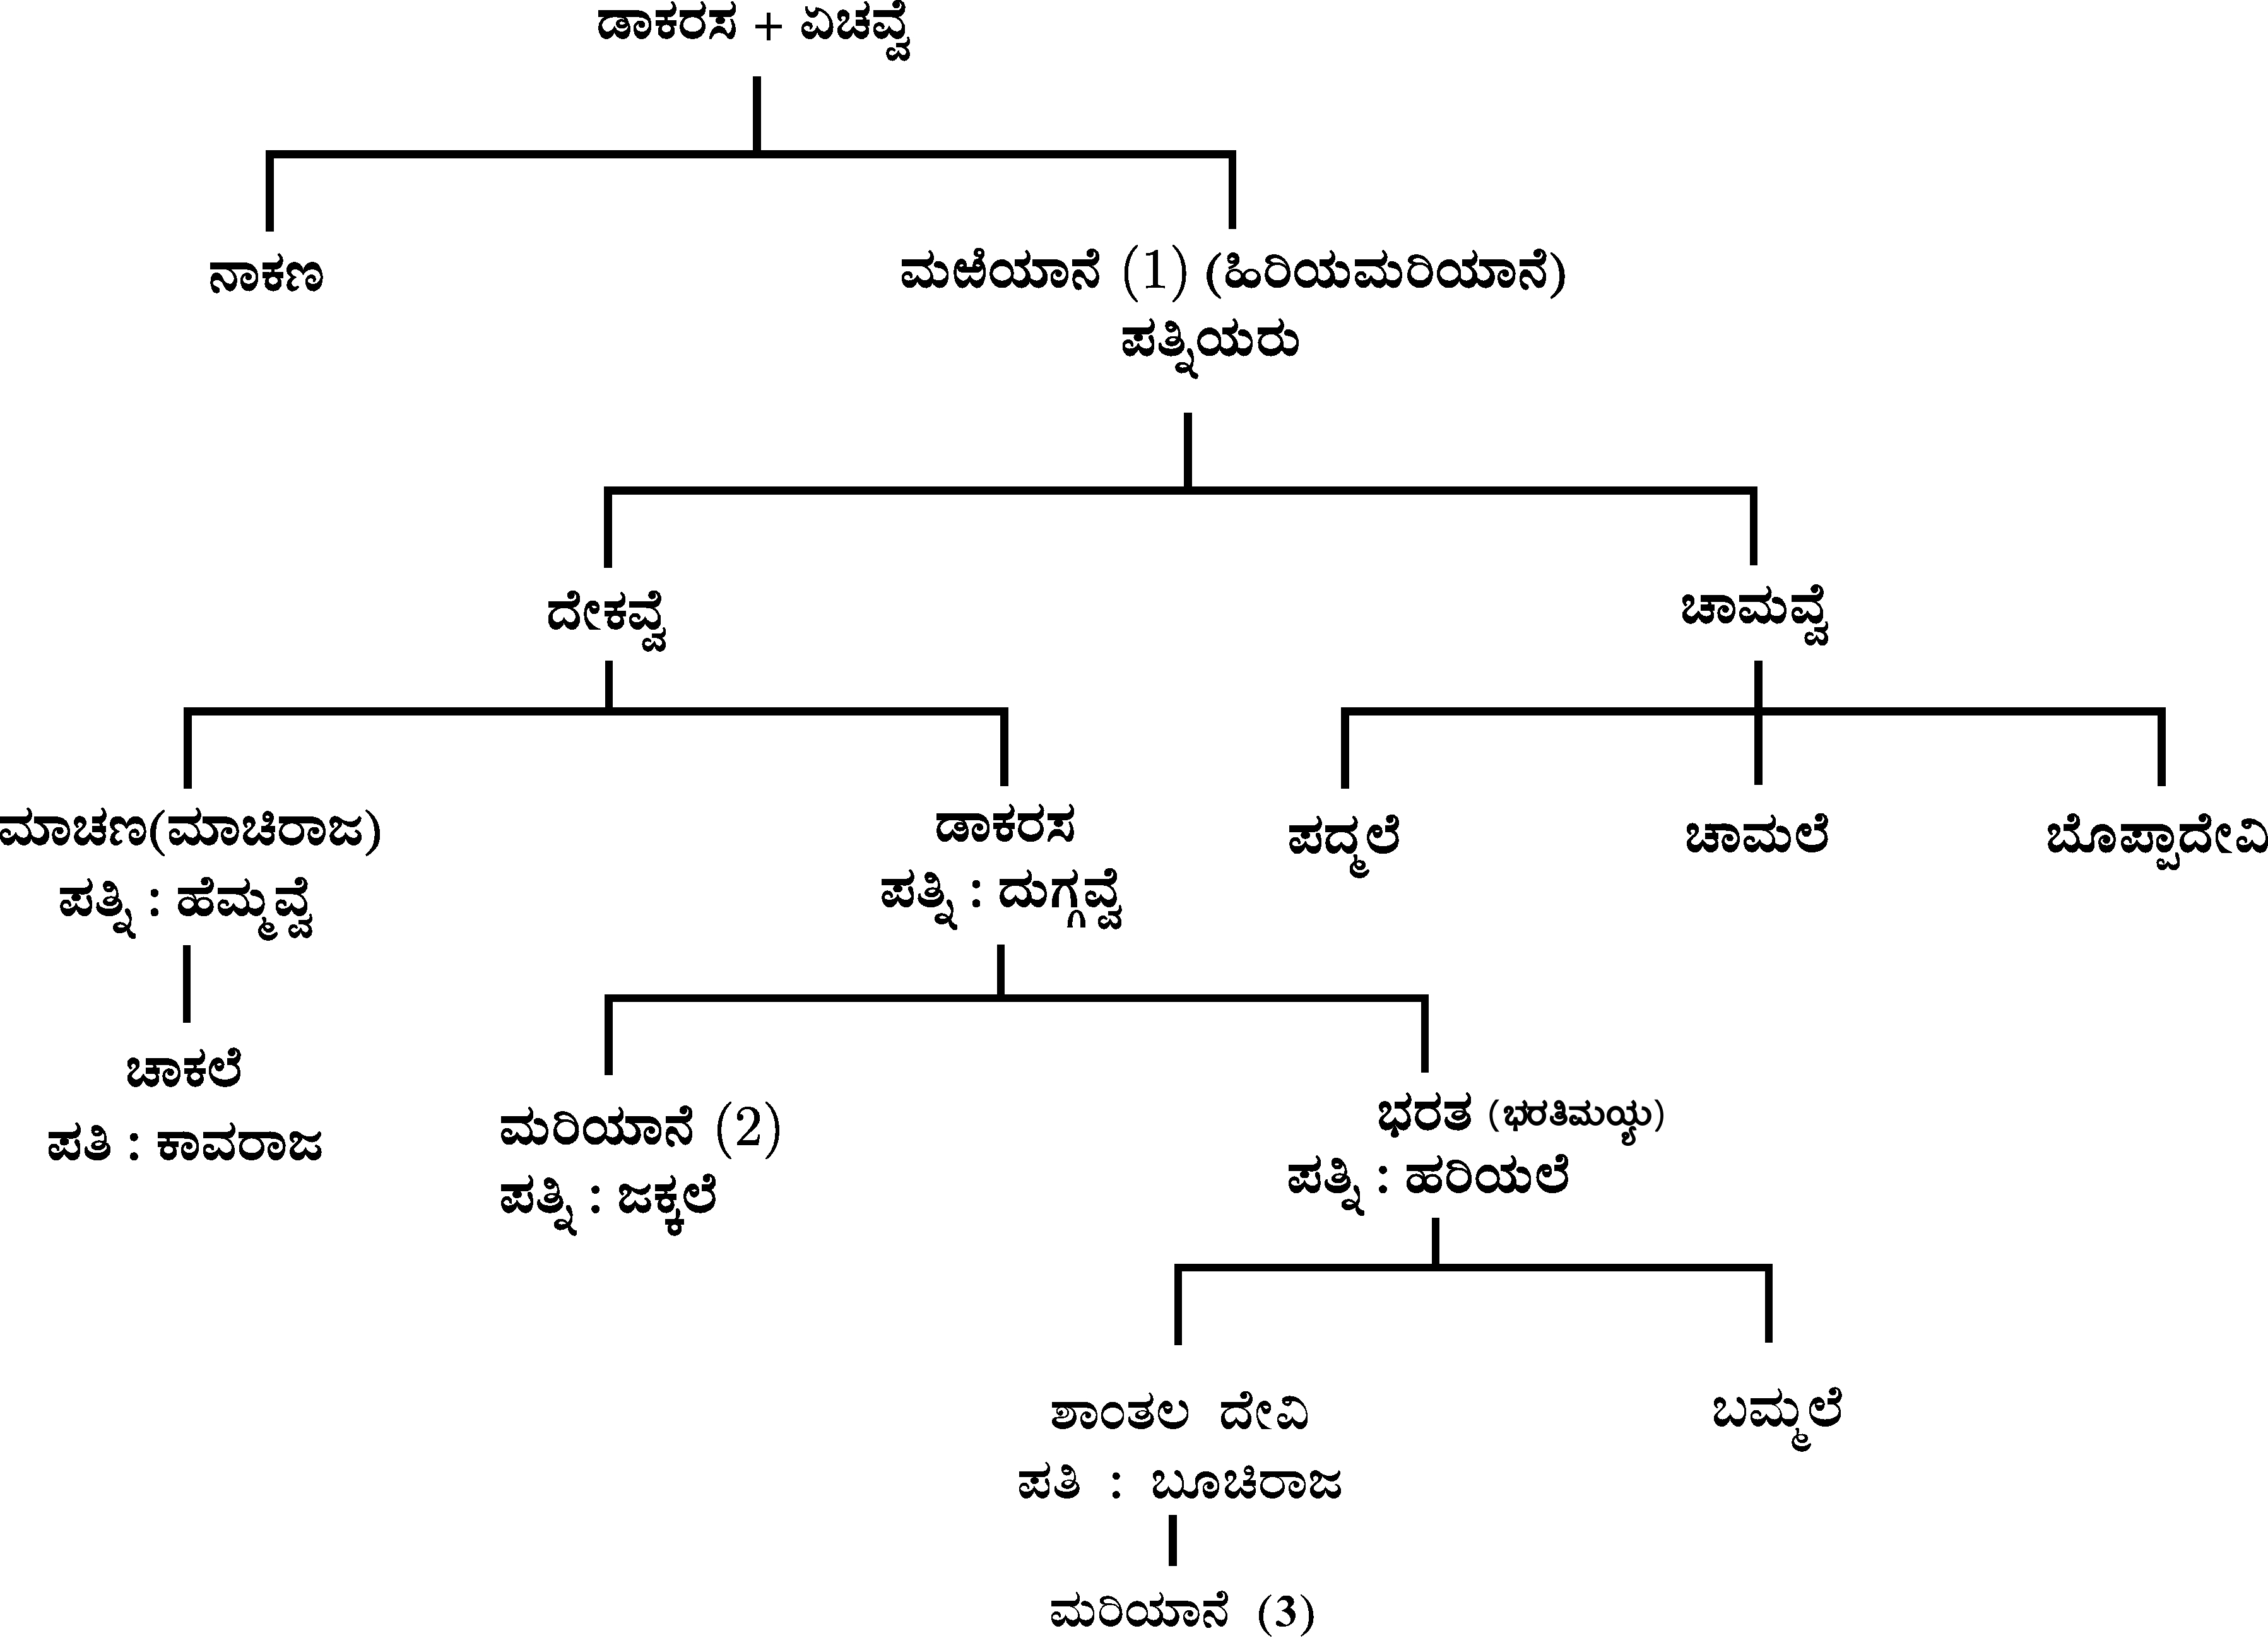
\includegraphics[scale=1.15]{images/chap3/chap3fig13.jpeg}
\end{figure}

\textbf{ಮಹಾಪ್ರಧಾನ\index{ಮಹಾಪ್ರಧಾನ} ಭರತಿಮಯ್ಯ\index{ಭರತ (ಭರತಿಮಯ್ಯ) ದಂಡನಾಯಕ} ಮತ್ತು ಬಾಹುಬಲಿ ದಂಡನಾಯಕರು\index{ಬಾಹುಬಲಿ ದಂಡನಾಯಕ} (1182\general{\enginline{-}}1183): }ಅಳೀಸಂದ್ರ\index{ಅಳಿಸಂದ್ರ (ಅಳೀಸಂದ್ರ)} ಮತ್ತು ಸಿಂಧಗೆರೆಯ\index{ಸಿಂಧಗೆರೆ} ಶಾಸನಗಳ ಡಾಕರಸ ಮತ್ತು ಮರಿಯಾನೆ ವಂಶವು ಹೊಯ್ಸಳರ ಇಮ್ಮಡಿ ಬಲ್ಲಾಳನ ಸೇವೆಯಲ್ಲಿ ಮುಂದುವರಿ\-ಯುತ್ತದೆ. ಎರಡನೆಯ ಮರಿಯಾನೆ\index{ಎರಡನೆಯ ಮರಿಯಾನೆ} ದಂಡನಾಯಕ ಮತ್ತು ಜಕ್ಕಲೆಗೆ\index{ಜಕ್ಕಲೆ} ನಾಲ್ಕು ಜನ ಮಕ್ಕಳು. ಬೊಪ್ಪ\index{ಬೊಪ್ಪ ಚಮೂಪ (ದಂಡನಾಯಕ - ದಂಡಾಧೀಶ)}, ಹೆಗ್ಗಡೆದೇವ (ಹೆಗ್ಗಡೆ ಪಾರ್ಶ್ವ)\index{ಹೆಗ್ಗಡೆದೇವ (ಹೆಗ್ಗಡೆ ಪಾರ್ಶ್ವ)} ಭರತಿಮಯ್ಯ\index{ಭರತ (ಭರತಿಮಯ್ಯ) ದಂಡನಾಯಕ} ಮತ್ತು ಬಾಹುಬಲಿ\index{ಬಾಹುಬಲಿ ದಂಡನಾಯಕ}. ಇವರಲ್ಲಿ ಭರತಿಮಯ್ಯ ಮತ್ತು ಬಾಹುಬಲಿ ದಂಡನಾಯಕರು ರಾಮ ಲಕ್ಷ್ಮಣರಂತಿದ್ದು, \textbf{ಇಮ್ಮಡಿ ಬಲ್ಲಾಳನ ಶ‍್ರೀಮನ್​ ಮಹಾಪ್ರಧಾನರು, ಸರ್ವಾಧಿಕಾರಿಗಳು\index{ಸರ್ವಾಧಿಕಾರಿ} ಮತ್ತು ಪ್ರಾಣಾಧಿಕಾರಿಗಳೂ\index{ಪ್ರಾಣಾಧಿಕಾರಿ}}ಆಗಿದ್ದರೆಂದು ಅಳಿಸಂದ್ರ ಶಾಸನ ತಿಳಿಸುತ್ತದೆ. ಭರತಿಮಯ್ಯನ ಹೆಂಡತಿ ಬೂಚಲೆ, ಬಾಹುಬಲಿಯ ಹೆಂಡತಿ ನಾಗಲದೇವಿ. ಇವರು ಕ್ರಿ.ಶ.1182 ರಲ್ಲಿ ಕುಮಾರ ವೀರನರಸಿಂಹನ (ಎರಡನೇ ನರಸಿಂಹ) ಜನ್ಮೋತ್ಸವದಂದು ತಮ್ಮ ಅನ್ವಯಕ್ಕೆ ಸೇರಿದ ಸಿಂಧಗೆರೆ\index{ಸಿಂಧಗೆರೆ}, ಬಗ್ಗವಳ್ಳಿ\index{ಬಗ್ಗವಳ್ಳಿ}, ಕಲುಕಣಿನಾಡ\index{ಕಲುಕಣಿ (ಕಲಿಕಣಿ-ಕಲ್ಕಣಿ-ಕಲ್ಕುಣಿ-ಕಲುಕರೆ) ನಾಡು} ದಡಿಗನಕೆರೆಗೆ\index{ದಡಗ (ದಡಿಗ, ದಡಿಗನಕೆರೆ)} ಸೇರಿದ ಅಣುವಸಮುದ್ರದ ಪ್ರಭುತ್ವವನ್ನು ಪಡೆದು, ಅಲ್ಲಿ ಒಂದು ಹೊಸ ಬಸದಿಯನ್ನು ನಿರ್ಮಿಸಿ ಆ ಬಸದಿಗೆ ಮತ್ತು ಚಾಕೇನ ಹಳ್ಳಿಯ ಬಸದಿಗೆ ದೇವಪೂಜೆ ಮತ್ತು ಆಹಾರದಾನಕ್ಕಾಗಿ ಗದ್ದೆ ಬೆದ್ದಲುಗಳನ್ನು ಕ್ರಿ.ಶ.1183 ರಲ್ಲಿ ದತ್ತಿಯಾಗಿ ಬಿಡುತ್ತಾರೆ.\endnote{ ಎಕ 7 ನಾಮಂ 72 ಅಳಿಸಂದ್ರ} ಭರತ ಬಾಹುಬಲಿಗಳು ಮರಿಯಾನೆ ದಂಡನಾಯಕ ಮತ್ತು ಜಕ್ಕಣಬ್ಬೆಯರ ಪುತ್ರರೆಂಬ ವಿಚಾರ ತಗಡೂರು ಶಾಸನದಲ್ಲೂ ಬಂದಿದೆ.\endnote{ ಎಕ 10 ಚರಾಪ 52 ತಗಡೂರು 12ನೇ ಶ.} ಪೆರ್ಗ್ಗಡೆ ಮಾಚಿರಾಜ\index{ಪೆರ್ಗ್ಗಡೆ ಮಾಚಿರಾಜ} ಮತ್ತು ಮರುದೇವಿಯರ\index{ಮರುದೇವಿ} ಮಗಳಾದ ಚಾಮಲೆಯು\index{ಚಾಮಲೆ} ತಗಡೂರಿನಲ್ಲಿ ಜಿನಾಲಯವನ್ನು ಕಟ್ಟಿಸಿದ ವಿಚಾರ ಈ ಶಾಸನದಲ್ಲಿದೆ. ಈ ಚಾಮವ್ವೆ ಹಿರಿಯ ಮರಿಯಾನೆಯ ಪತ್ನಿ, ಅಂದರೆ ಭರತಿಮಯ್ಯ ಮತ್ತು ಬಾಹುಬಲಿಯರ ಅಜ್ಜಿ. ಚಾವುಂಡ\index{ಚಾವುಂಡ} ಮತ್ತು ಬೂಚಿಯಣ್ಣ\index{ಬೂಚಿಯಣ್ಣ} ಇವಳ ಸೋದರರೆಂದು ಶಾಸನ ಹೇಳುತ್ತದೆ. ಕರಗುಂದ ಶಾಸನದಲ್ಲೂ ಕೂಡಾ ಮರಿಯಾನೆ ಮತ್ತು ಭರತಿಮಯ್ಯರ ಪ್ರಸ್ತಾಪ ಇದೆ.\endnote{ ಎಕ 10 ಅರ 241 ಕರಗುಂದ 1158} ಮರಿಯಾನೆಯ ಮಗಳು ಬಮ್ಮಲ ದೇವಿಯ ಪತಿ ಪಾರ್ಶ್ವನಾಥ ಹಾಕಿಸಿರುವ ಶಾಸನ ಇದಾಗಿದೆ. ತಂದೆ ಮರಿಯಾನೆ, ಕಿರಿಯಯ್ಯ (ಚಿಕ್ಕಪ್ಪ) ಭರತಿಮಯ್ಯ ಎಂದು ಬಮ್ಮಲದೇವಿಯನ್ನು ವರ್ಣಿಸುವ ಪದ್ಯದಲ್ಲಿ ಹೇಳಿದೆ. ಎರಡನೇ ಮರಿಯಾನೆಗೆ ಬಮ್ಮಲದೇವಿ ಎಂಬ ಮಗಳಿದ್ದ ವಿಚಾರ ಈ ಶಾಸನದಿಂದ ತಿಳಿಯುತ್ತದೆ. ಅಳಿಸಂದ್ರ ಶಾಸನ ಮತ್ತು ಪೂರ್ವೋಕ್ತ ಶಾಸನದ ಪ್ರಕಾರ ಇವರ ಎರಡನೆಯ ಮರಿಯಾನೆಯ ಮುಂದುವರಿದ ವಂಶಾವಳಿ ಈ ಕೆಳಗಿನಂತಿದೆ.

\begin{figure}[H]
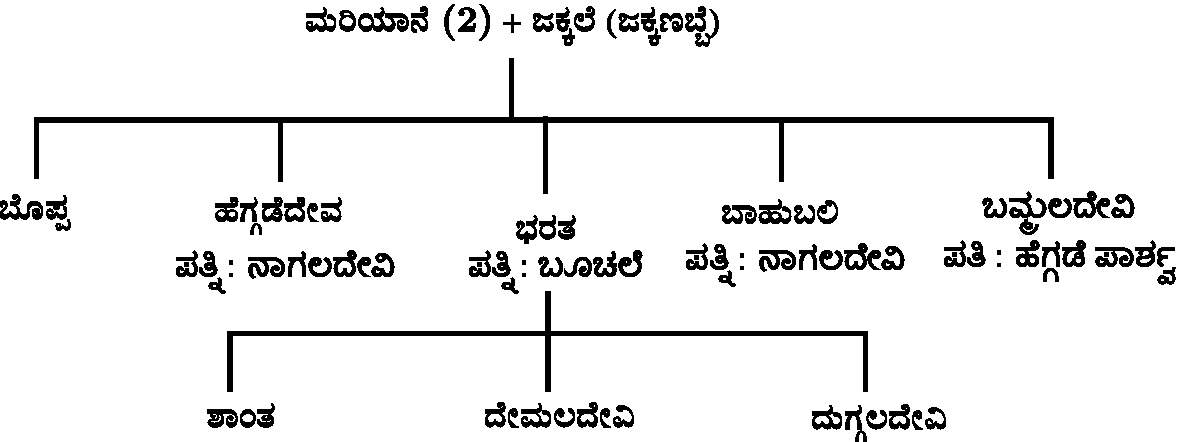
\includegraphics[scale=1.15]{images/chap3/chap3fig14.jpeg}
\end{figure}

\textbf{ಮಹಾಪ್ರಧಾನ ಸರ್ವಾಧಿಕಾರಿ ಮಹಾಪಸಾಯತ, ತಂತ್ರಾಧಿಷ್ಠಾಯಕ ಹೆಗ್ಗಡೆ ಸುರಿಗೆ ನಾಗಯ್ಯ\index{ಸುರಿಗೆಯ (ಸುರಗಿಯ) ನಾಗಯ್ಯ (ನಾಗಿದೇವ, ನಾಗಣ್ಣ)} (1140\general{\enginline{-}}1175):} ಸುರಿಗೆ ನಾಗಯ್ಯನು ವಿಷ್ಣುವರ್ಧನ, ನಾರಸಿಂಹ ಮತ್ತು ಇಮ್ಮಡಿ ಬಲ್ಲಾಳನ ಕಾಲದಲ್ಲಿ ಅಧಿಕಾರದಲ್ಲಿದ್ದನು. ಸುರಿಗೆಕಾರ\index{ಸುರಿಗೆಕಾರ} ಎಂಬ ಅಧಿಕಾರಿಯ ಪ್ರಸ್ತಾಪ ಹೊಯ್ಸಳರ ಶಾಸನಗಳಲ್ಲಿ ಬರುತ್ತದೆ. ಸುರಿಗೆಯ ಗಂಗಣ್ಣ,\endnote{ ಎಕ 8 ಹಾಸನ 98 ಹೊನ್ನಾವರ 1158} ಸುರಿಗೆಯ ವಿಜಯಾದಿತ್ಯ ಹೆಗ್ಗಡೆ.\endnote{ ಎಕ 8 ಹಾಸನ 196 ಗೊರೂರು 1167} ಮುಂತಾದವರು ಶಾಸನೋಕ್ತರಾಗಿದ್ದಾರೆ. ಚಾಮುಂಡರಾಯನೆಂಬುವವನು ಸುರಿಗೆಯ ಅಂಕಕಾರನಾಗಿದ್ದನೆಂದು\index{ಸುರಿಗೆಯ ಅಂಕಕಾರ}\break ಹೇಳಿದೆ.\endnote{ ನಾಗಯ್ಯ ಡಾ॥ ಜೆ.ಎಂ., ಆರನೆಯ ವಿಕ್ರಮಾದಿತ್ಯನ ಶಾಸನಗಳು, ಪುಟ 241} ವಿಕ್ರಮಾದಿತ್ಯನು ಹೆರ್ಮ್ಮಾಡಿ ದೇವನೆಂಬುವವನಿಗೆ ಸುರಿಗೆವಿಡಿವ ಅಧಿಕಾರವನ್ನು ನೀಡಿ ಮಹಾಮಾತ್ಯ ಪದವಿಯನ್ನು ನೀಡಿದನೆಂದು, ಸುರಿಗೆಯ ಪೆರ್ಮಾಡಿ ದೇವನ ತಂದೆ ಮಹಾದೇವ ದಂಡನಾಯಕನಿಗೆ ವಿಕ್ರಮಾದಿತ್ಯನು ಸುರಿಗೆವಿಡಿವ ಅಧಿಕಾರವನ್ನು ನೀಡಿದ್ದನೆಂದು ತಿಳಿದುಬರುತ್ತದೆ.\endnote{ ಅದೇ ಪುಟ 344} ಸುರಿಗೆಯ ಲೆಂಕಮಹಾದೇವ, ಸುರಿಗೆಯ ಪೆರ್ಮಾಡಿ, ಸುರಿಗೆಯ ನಾಗರಸ ಈ ಅಧಿಕಾರಿಗಳ ಉಲ್ಲೇಖ ವಿಕ್ರಮಾದಿತ್ಯನ ಶಾಸನಗಳಲ್ಲಿ ಬರುತ್ತದೆ.\endnote{ ಅದೇ, ಪುಟ344-46}

ಸುರಿಗೆ ನಾಗಯ್ಯನೂ ಇಂತಹ ಅಧಿಕಾರಿಯಾಗಿದ್ದು, ಹಂತಹಂತವಾಗಿ ಮೇಲೇರಿರುವುದು ತಿಳಿದುಬರುತ್ತದೆ. ಮೊದಲಿಗೆ ಈತನು ಮಹಾಪ್ರಧಾನ ಹೆಗ್ಗಡೆ ಮತ್ತು ಚತ್ರಾಧಿಕಾರಿಯಾಗಿದ್ದನು\index{ಚತ್ರಾಧಿಕಾರಿ}. ಆನಂತರ ಮಹಾಪ್ರಧಾನ ಸರ್ವಾಧಿಕಾರಿಯಾದನು. ಸುರಿಗೆ ನಾಗಯ್ಯನ ಕೈಕೆಳಗಿನ ಅಧಿಕಾರಿಯಾದ ಸುಂಕದ ನರಣ(ನಾರಾಯಣ) ಹೆಗ್ಗಡೆಯು\index{ಸುಂಕದ ನರಣ(ನಾರಾಯಣ) ಹೆಗ್ಗಡೆ} ತೊಳಂಚೆಯ ಮಹಾದೇವರಿಗೆ\index{ತೊಳಂಚೆಯ ಮಹಾದೇವ} ದತ್ತಿ ಬಿಡುತ್ತಾನೆ.\endnote{ ಎಕ 6 ಕೃಪೇ 54 ತೊಣಚಿ 12ನೇ ಶ.} ಇದು ಸುರಿಗೆ ನಾಗಯ್ಯನ ಮೊದಲ ಶಾಸನವೆಂದು ಹೇಳಬಹುದು. ಸುರಿಗೆನಾಗಯ್ಯನ ಆದೇಶದಂತೆ ಕೊಮ್ಮಣ್ಣ ಪೆರ್ಗಡೆಯು\index{ಕೊಮ್ಮಣ್ಣ ಪೆರ್ಗಡೆ} ಅರಕೆರೆಯ\index{ಅರಕೆರೆ} ಕೇಶವ ದೇವರಿಗೆ ಮಗ್ಗದ ತೆರಿಗೆಗಳನ್ನು ದತ್ತಿಯಾಗಿಬಿಟ್ಟನು.\endnote{ ಎಕ 6 ಶ‍್ರೀಪ 104 ಅರಕೆರೆ 12ನೇ ಶ.} ಈತನ ಕೈಕೆಳಗೆ ಸುಂಕದ ಹೆಗ್ಗಡೆಗಳು\index{ಸುಂಕದ ಹೆಗ್ಗಡೆ} ಕೆಲಸ ಮಾಡುತ್ತಿದ್ದರು, ಎಂದರೆ ಈತನು ಸಚಿವನಿಗೆ ಸಮಾನವಾದ ಪದವಿಯನ್ನು ಹೊಂದಿದ್ದನೆಂದು ಊಹಿಸಬಹುದು. ಇಲ್ಲಿಂದ ಮುಂದೆ ಅವನನ್ನು ಶಾಸನಗಳು ಶ‍್ರೀಮನ್​ಮಹಾಪ್ರಧಾನನೆಂದು ಕರೆದಿವೆ. ಶ‍್ರೀಮನ್​ಮಹಾಪ್ರಧಾನ ಚತ್ರಾಧಿಕಾರಿ ಹೆಗ್ಗಡೆ ಸುರಿಗೆ ನಾಗಯ್ಯನು ಮೇಲುಕೋಟೆ\index{ಮೇಲುಕೋಟೆ} ನಾರಾಯಣಸ್ವಾಮಿ ದೇವಾಲಯದ ರಂಗಮಂಟಪವನ್ನು ನಿರ್ಮಿಸಿದ್ದಾನೆ.\endnote{ ಎಕ 6 ಪಾಂಪು 124 ಮೇಲುಕೋಟೆ 12ನೇ ಶ.} ವಿಷ್ಣುವರ್ಧನನ ಆದೇಶದಿಂದ ಮಹಾಪ್ರಧಾನ ತಂತ್ರಾಧಿಷ್ಟಾಯಕ ಮಹಾಪಸಾಯಿತ ಹೆಗ್ಗಡೆ ಸುರಿಗೆ ನಾಗಯ್ಯನು ತೊಂಡನೂರಿನ\index{ತೊಂಡನೂರು} ಲಕ್ಷ್ಮೀನಾರಾಯಣ ದೇವಾಲಯದ ಓಲಗಸಾಲೆಯನ್ನು\index{ಓಲಗಸಾಲೆ} ನಿರ್ಮಿಸಿದನು.\endnote{ ಎಕ 6 ಪಾಂಪು 73 ತೊಣ್ಣೂರು 12ನೇ ಶ.} ಈ ಹೊತ್ತಿಗೆ ಇವನು ಎಲ್ಲ ಪದವಿಗಳನ್ನು ಅಲಂಕರಿಸಿರುವುದನ್ನು ನೋಡಬಹುದು.

ಇಮ್ಮಡಿ ಬಲ್ಲಾಳನ ಕಾಲದಲ್ಲೂ ಇವನು ಮಹಾಪ್ರಧಾನನಾಗಿ ಮುಂದುವರಿದನು. ಶ‍್ರೀಮನ್​ ಮಹಾಪ್ರಧಾನ ಸರ್ವಾಧಿಕಾರಿ, ಮಹಾಪಸಾಯತ, ತಂತ್ರಾಧಿಷ್ಠಾಯಕ, ಹೆಗ್ಗಡೆ ಸುರಿಗೆ ನಾಗಯ್ಯನ ಆದೇಶದಂತೆ ನಾಯಕಹೆಗ್ಗಡೆ ಮಾರಣ್ಣನು ಅನಾದಿ ಅಗ್ರಹಾರವಾದ ತೊಂಡನೂರ ನಡುವಣ ದೇವಾಲಯಕ್ಕೆ\index{ತೊಂಡನೂರ ನಡುವಣ ದೇವಾಲಯ} ವಿರ್ರಿರುಂದ ಪೆರುಮಾಳೆ ದೇವಾಲಯಕ್ಕೆ, ಎಲೆ ತೋಟಗಳನ್ನು ದತ್ತಿಯಾಗಿ ನೀಡಿದನು.\endnote{ ಎಕ 6 ಪಾಂಪು 79 ತೊಣ್ಣೂರು 1175} ಈ ಶಾಸನದಲ್ಲಿ ನಾಗಯ್ಯನಿಗೆ ಸಕಲ ಪದವಿಗಳನ್ನೂ ಆರೋಪಿಸಲಾಗಿರುವುದನ್ನು ನೋಡಬಹುದು. ಶ‍್ರೀಮನ್​ ಮಹಾಪ್ರಧಾನ, ಸರ್ವಾಧಿಕಾರಿ\index{ಸರ್ವಾಧಿಕಾರಿ}, ಶ‍್ರೀಕರಣದಧಿಷ್ಟಾಯಕ\index{ಶ‍್ರೀಕರಣದಧಿಷ್ಟಾಯಕ}, ಪರಮವಿಶ್ವಾಸಿ\index{ಪರಮವಿಶ್ವಾಸಿ}, ಹಿರಿಯ ಮಾಣಿಕ್ಯಭಂಡಾರಿ ನಾಗಯ್ಯಗಳ\index{ಹಿರಿಯ ಮಾಣಿಕ್ಯಭಂಡಾರಿ ನಾಗಯ್ಯ} ಮಾವ ಮಾದಿಗವುಡನ\index{ಮಾದಿಗಉಡ (ಗವುಡ - ಗೌಡ)} ಪ್ರಸ್ತಾಪ ವೀರಬಲ್ಲಾಳನ ಕಾಲದ ಮುದುಡಿಯ\index{ಮುದುಡಿ} ವೀರಗಲ್ಲಿನಲ್ಲಿದೆ.\endnote{ ಎಕ 10 ಅರ 221 ಮುದುಡಿ 13ನೇ ಶ.} ಈತನೂ ಕೂಡಾ ಸುರಿಗೆ ನಾಗಯ್ಯನೇ ಆಗಿದ್ದು ಮಾಣಿಕ್ಯ ಭಂಢಾರಿಯ ಹುದ್ದೆಯನ್ನು ಹೆಚ್ಚುವರಿಯಾಗಿ ಪಡೆದಿದ್ದಾನೆ. ಸುರಿಗೆ ಚೆಲ್ವಡರಾಯನೆಂಬ\index{ಸುರಿಗೆಯ ಚೆಲ್ವೊಡರಾಯ} ಪುರಾತನ ಶೈವನೊಬ್ಬನ ಉಲ್ಲೇಖ ಸಂಗನಬಸವನ (ಬಸವಣ್ಣನವರು) ಜೊತೆಗೆ ಮರಡಿಪುರ\index{ಮರಡಿಪುರ} ಶಾಸನದಲ್ಲಿದೆ.\endnote{ ಎಕ 7 ಮಂ 13 ಮರಡಿಪುರ 1280} ಸುರಿಗೆ ನಾಗಯ್ಯ ಈ ಶೈವ ಪಂಗಡಕ್ಕೆ ಸೇರಿದವನಿರಬಹುದು. ವಿಜಯನಗರದ ಕಾಲದ ಒಂದು ಶಾಸನದಲ್ಲಿ ಸುರಗಿ ದೇವಪ್ಪ ನಾಯಕರು\index{ಸುರಗಿಯ ದೇವಪ್ಪನಾಯಕ} ಕುಡಗಬಾಳ\index{ಕುಡುಗುಬಾಳು} ರಾಮಲಿಂಗದೇವರಿಗೆ ದತ್ತಿಬಿಟ್ಟ ವಿಚಾರ ಬರುತ್ತದೆ.\endnote{ ಎಕ 7 ನಾಮಂ 165 ಕುಡುಗಬಾಳು 1640} ಈತನೇನಾದರೂ ಸುರಿಗೆ ನಾಗಯ್ಯನ ವಂಶದವನೇ ತಿಳಿಯದು.

\textbf{ಮಹಾಪ್ರಧಾನ ದಂಡನಾಯಕ\index{ಮಹಾಪ್ರಧಾನ ದಂಡನಾಯಕ} ಪುಣಿಸಮಯ್ಯ\index{ಪುಣಿಸಮಯ್ಯ} (1116\general{\enginline{-}}17): }ವಿಷ್ಣುವರ್ಧನನ\index{ವಿಷ್ಣುವರ್ಧನ (ದೇವರು) (ಹೊಯ್ಸಳರ ದೊರೆ)} ಮಹಾಪ್ರಧಾನ ದಂಡನಾಯಕ\break ಪುಣಿಸಮಯ್ಯನು ನಾಡಮಾಣಿಕದೊಡಲೂರಿನಲ್ಲಿ (ಇಂದಿನ ಬಸ್ತಿ) ಹೊಯ್ಸಳ ಜಿನಾಲಯವನ್ನು\index{ಹೊಯ್ಸಳ ಜಿನಾಲಯ} ಮಾಡಿಸಿ ಅದಕ್ಕೆ ಮೋದೂರು ನಾಡಿನ ನಾಡಮಾಣಿಕದೊಡಲೂರನ್ನು ಹಾಗೂ ಮಾವಿನಕೆರೆಯನ್ನೂ ಸರ್ವಬಾಧಾಪರಿಹಾರವಾಗಿ ಬಿಟ್ಟನು.\endnote{ ಎಕ 6 ಕೃಪೇ 107 ಬಸ್ತಿ 1117} ಪುಣಿಸಮಯ್ಯ ದಂಡನಾಯಕನ ವಂಶವೃಕ್ಷ ಹಾಗೂ ಇತರ ವಿವರಗಳು ಚಾಮರಾಜನಗರದ\index{ಚಾಮರಾಜನಗರ} ಪಾರ್ಶ್ವನಾಥ ಬಸದಿಯ ಶಾಸನದಲ್ಲಿದೆ.\endnote{ ಎಕ 4 ಚಾನ 2 ಚಾಮರಾಜನಗರ 1116}\textbf{ಈ ಶಾಸನದಲ್ಲಿ ಪುಣಿಸಮಯ್ಯನು ಸಂಧಿವಿಗ್ರಹಿ\index{ಸಂಧಿವಿಗ್ರಹಿ} ದಂಡನಾಯಕನಾಗಿದ್ದನೆಂದು ಹೇಳಿದೆ. ಒಂದು ವರ್ಷದ ನಂತರದ ಬಸ್ತಿ ಶಾಸನದಲ್ಲಿ ಇವನನ್ನು ಮಹಾಪ್ರಧಾನ ದಂಡನಾಯಕ ಪುಣಿಸಮಯ್ಯನೆಂದುಹೇಳಿದೆ. ಆದುದರಿಂದ ಇವನು ದಂಡನಾಯಕ ಸಂಧಿವಿಗ್ರಹಿ ಪದವಿಯಿಂದ, ಮಹಾಪ್ರಧಾನ ದಂಡನಾಯಕನ ಹುದ್ದೆಗೆ ಬಡ್ತಿಯನ್ನು ಪಡೆದಿದ್ದಾನೆಂಬುದು ಸ್ಪಷ್ಟವಾಗಿದೆ.} ವಿಷ್ಣುವರ್ಧನನು ತಲಕಾಡು ವಿಜಯವನ್ನು ಸಾಧಿಸಿ ಕೋಳಾಲಪುರದ\index{ಕೋಳಾಲಪುರ} ಬೀಡಿನಲ್ಲಿದ್ದಾಗ, ಪುಣಿಸಮಯ್ಯನು ಚಾಮರಾಜನಗರದಲ್ಲಿ ಬಸದಿಯನ್ನು ನಿರ್ಮಿಸಿ ಶಾಸನವನ್ನು ಹಾಕಿಸಿದನು.

ಪುಣಿಸಮಯ್ಯನ ಗುರು ದ್ರಾವಿಡಾನ್ವಯದ\index{ದ್ರಾವಿಡಾನ್ವಯ} ಅಜಿತಮುನಿ\index{ಅಜಿತಮುನಿ}. ತಲಕಾಡು ವಿಜಯದ ವೇಳೆಗೆ ಪುಣಿಸಮಯ್ಯನು\break \textbf{“ಕೊಂಗರನಡಗಿಸಿ, ಪೊಲುವರಂ ಪೊರಳ್ಚಿ ಮಾಣದ ಮಲೆಯಾಳಗಮಿಡಿಪಿ ಕಾಳನ್ರಿಪಾಳನ ತೋಳಬಿಂಕಮಂ ಬೆದರಿಸಿ ಪೊಕ್ಕು ನಿಲಿಸಿಳೆಯಂ, ನೀಳಾದ್ರಿಯಂ ಕೊಂಡು, ಮಲೆಯಾಳರಂ ಕದನದೊಳ್​ ಬೆಂಕೊಂಡು, ತತ್ಸಾಹಸಾಭ್ಯುದಯಂ ಕೈಕೊಳೆ\general{\break } ಕೇರಳಾಧಿಪತಿಯಾಗಿರ್ದೆ ಬಯಲ್ನಾಡನಂ ಪದಪಿಂ ಕಾಣಿಸಿ ಕೊಂಡನಿಂತು ಪುಣಿಸಶ‍್ರೀ ದಂಡನಾಥಾಧಿಪ”} ಎಂದು ಶಾಸನವು ಇವನ ವಿಜಯಗಳನ್ನು ಬಣ್ಣಿಸಿದೆ. ಗಂಗವಾಡಿಯ ತೊಂಭತ್ತರುಸಾಸಿರದ\index{ಗಂಗವಾಡಿ ತೊಂಭತ್ತರುಸಾಸಿರ} ಬಸದಿಗಳನ್ನು ಅಲಂಕರಿಸಿದ ಸಂಧಿವಿಗ್ರಹಿ ದಂಡನಾಯಕ ಪುಣಿಸಮಯ್ಯನು, ಎಣ್ಣೆನಾಡ ಅರೆಕೊಠಾರದಲ್ಲಿ (ಚಾಮರಾಜನಗರ)\index{ಅರೆಕೊಠಾರ (ಚಾಮರಾಜನಗರ)} ತ್ರಿಕೂಟ ಬಸದಿಯನ್ನು\index{ತ್ರಿಕೂಟ ಬಸದಿ} ಮಾಡಿಸಿ ಅದಕ್ಕೆ ಅನೇಕ ದತ್ತಿಗಳನ್ನು ಬಿಟ್ಟನು. ಇವನ ತಾತ ಪುಣಿಸಮ್ಮ ಚಮೂಪನು ಮಹಾಮಾತ್ಯ ಕುಲೋದ್ಭವನೂ \textbf{“ಸಕಲ ಶಾಸನ ವಾಚಕ ಚಕ್ರವರ್ತಿ\index{ಸಕಲ ಶಾಸನ ವಾಚಕ ಚಕ್ರವರ್ತಿ}”}ಯೂ ಆಗಿದ್ದನೆಂದು ಈ ಶಾಸನದಲ್ಲಿ ಹೇಳಿರುವುದು ವಿಶೇಷ. ಪುಣಿಸಮಯ್ಯನ ವಂಶವೃಕ್ಷವನ್ನು ನೀಡುವ ಇನ್ನೊಂದು ಶಾಸನ ಬೇಲೂರು ಚೆನ್ನಕೇಶವದೇವಾಲಯದ ಆವರಣದಲ್ಲಿರುವ ನಾಗನಾಯಕನ ಮಂಟಪದಲ್ಲಿದೆ.\endnote{ ಎಕ 9 ಬೇಲೂರು 44 ಬೇಲೂರು 12ನೇ ಶ.} ಬಹುಶಃ ಈ ಮಂಟಪವನ್ನು ಪುಣಿಸದಂಡನಾಥನು ಕಟ್ಟಿಸಿರಬಹುದು. ಇಲ್ಲಿಯೂ ಒಂದನೇ ಪುಣಸಮಯ್ಯನನ್ನು ಚಮೂಪ ಮತ್ತು ಶಾಸನವಾಚಕಚಕ್ರವರ್ತಿ ಎಂದು ಕರೆದಿದೆ. ಎರಡನೇ ಪುಣಿಸ ದಂಡನಾಥನನ್ನು ಚಾಮ ಚಮೂಪ ಸಂಭವ ಎಂದು ಹೇಳಿದೆ. ಇದೇ ತಾಲ್ಲೂಕಿನ ಬಸ್ತಿಹಳ್ಳಿಯಲ್ಲಿರುವ ಪಾರ್ಶ್ವನಾಥ ಜಿನಾಲಯವನ್ನೂ ಇವನೇ ಕಟ್ಟಿಸಿರಬಹುದು. ಇಲ್ಲಿಯೂ ದ್ರಮಿಳಸಂಘದ ಗುರುಗಳ ಉಲ್ಲೇಖವಿದ್ದು, ಇದನ್ನು ಪುಣಿಸ ಜಿನಾಲಯ ಎಂದು ಕರೆದಿದೆ.\endnote{ ಎಕ 9 ಬೇಲೂರು 400 ಬಸ್ತಿಹಳ್ಳಿ 12ನೇ ಶ.} ಪುಣಿಸ ದಂಡನಾಥನ ವಂಶವೃಕ್ಷ ಈ ಕೆಳಗಿನಂತಿದೆ.

\begin{figure}[H]
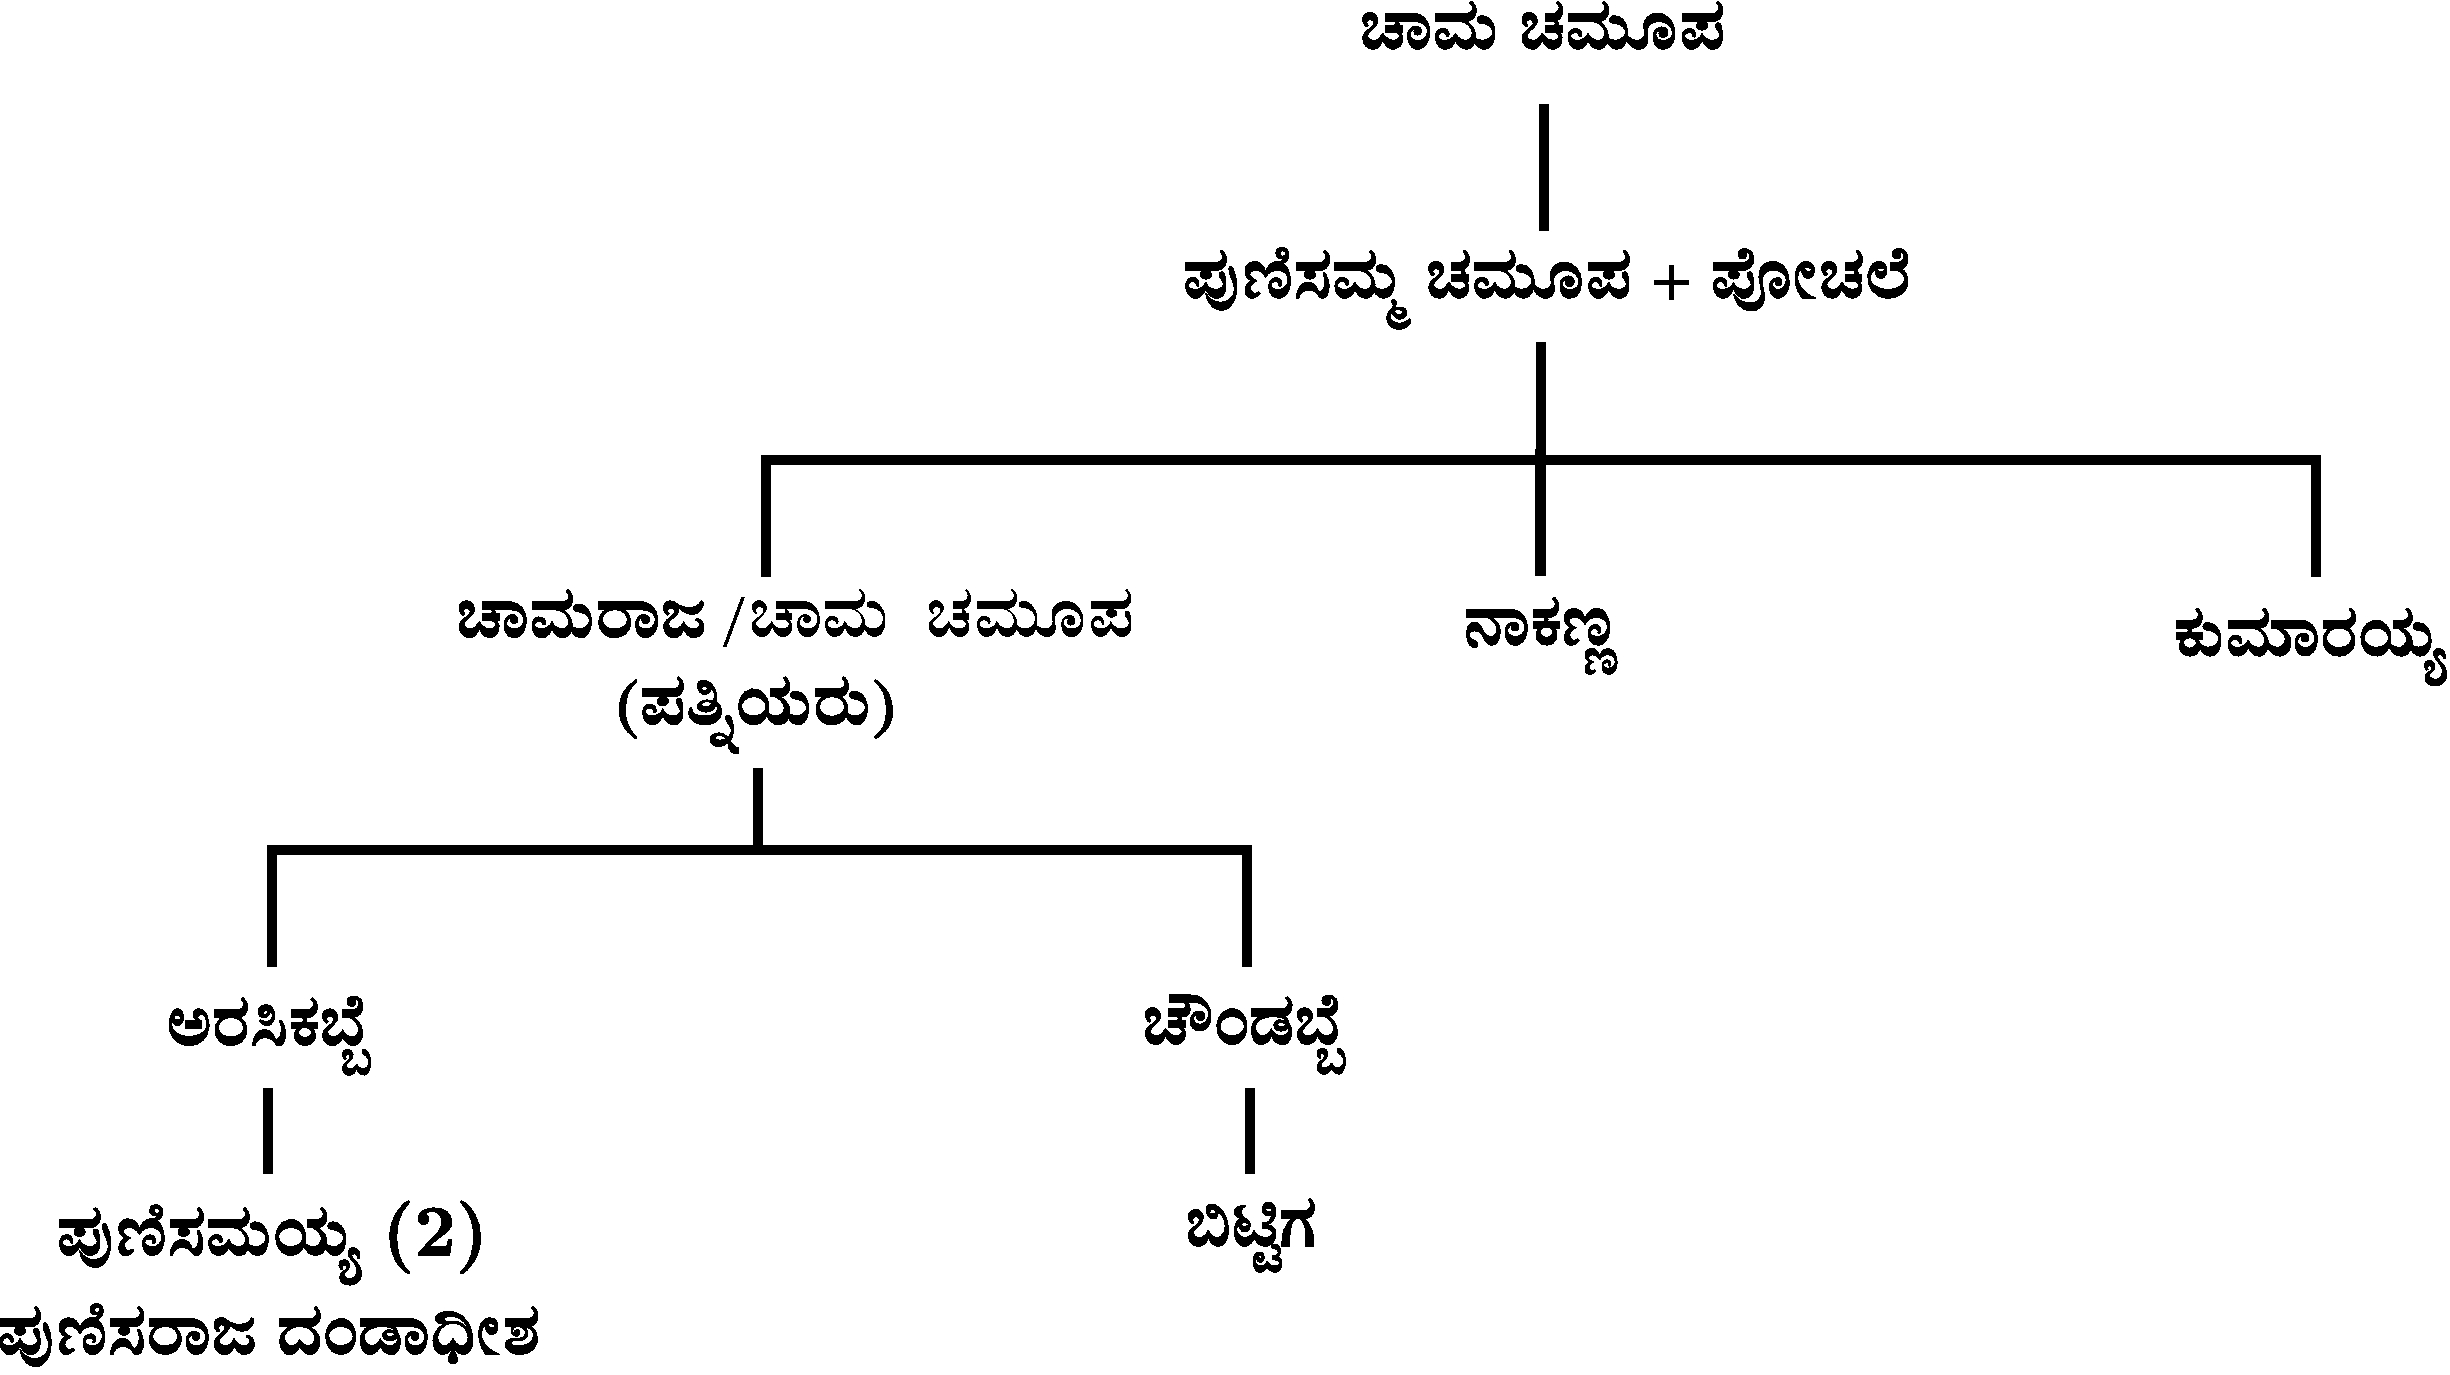
\includegraphics[scale=1.15]{images/chap3/chap3fig16.jpeg}
\end{figure}

\textbf{ಮಹಾಪ್ರಧಾನ ದಂಡನಾಯಕ ಲಿಂಗಪಯ್ಯ\index{ಲಿಂಗಪಯ್ಯ (ಲಿಂಗಪ್ಪಯ್ಯ)} (1118):} ಮಹಾಪ್ರಧಾನ ದಂಡನಾಯಕ ಲಿಂಗಪಯ್ಯನು,\break ವಿಷ್ಣುವರ್ಧನನು ತಲಕಾಡಿನಲ್ಲಿದ್ದಾಗ ಅವನಿಗೆ ವಿನಂತಿ ಮಾಡಿ ಕಂನಗೊಂಡೇಶ್ವರ\index{ಕಂನಗೊಂಡೇಶ್ವರ} ದೇವರಿಗೆ ಮತ್ತು ಕಾವೇರಿ\index{ಕಾವೇರಿ (ನದಿ-ಹೊಳೆ)} ತಡಿಯಲ್ಲಿದ್ದ ಕಣ್ನಂಬಾಡಿಯ ಮಹಾದೇವರಿಗೆ\index{ಕಣ್ನಂಬಾಡಿಯ ಮಹಾದೇವ} ದತ್ತಿಯನ್ನು ಬಿಡಿಸುತ್ತಾನೆ.\endnote{ ಎಕ 6 ಪಾಂಪು 41 ಕನ್ನಂಬಾಡಿ 1118 ಏಪ್ರಿಲ್​ 25} ಈ ದತ್ತಿಯನ್ನು ಹಿಂದೆ ಕನ್ನರದೇವನು (ಮೂರನೆಯ ಕೃಷ್ಣ)\index{ಕನ್ನರದೇವ (ಮೂರನೆಯ ಕೃಷ್ಣ)} ಬಿಟ್ಟಿದ್ದನೆಂದು ಅದು ಈ ದೇವರಿಗೆ ಸಲ್ಲುವುದೆಂದು ಲಿಂಗಪಯ್ಯನು ಬಿನ್ನಹ ಮಾಡಿದಂತೆ ಶಾಸನದಲ್ಲಿ ಹೇಳಿದೆ. ಶಾಸನವನ್ನೂ ತಲಕಾಡು ವಿಜಯದ ನಂತರ ಹಾಕಿಸಿರಬಹುದು.

\textbf{ಮಹಾಪ್ರಧಾನ ದಂಡನಾಯಕ ಸರ್ವಾಧಿಕಾರಿ ಬಿಟ್ಟಿಮಯ್ಯ\index{ಬಿಟ್ಟಿಮಯ್ಯ} (1136\general{\enginline{-}}1167):} ಬಿಟ್ಟಿಮಯ್ಯನು ಒಂದನೇ ನರಸಿಂಹನ ಶ‍್ರೀಮನ್ಮಹಾಪ್ರಧಾನ ದಂಡನಾಯಕನಾಗಿದ್ದನು. ಬಿಟ್ಟಿಮಯ್ಯನ ಆಜ್ಞೆಯ ಮೇರೆಗೆ ಮಾದಿವೆಗ್ಗಡೆಯು ಹಿರಿಯ ಅರಸನಕೆರೆಯ\index{ಹಿರಿಯ ಅರಸ(ಸಿ)ನಕೆರೆ} ಮಾಧವದೇವರಿಗೆ, ಮಾಧವಚೋಳನಹಳ್ಳಿಯ\index{ಮಾಧವಚೋಳಯನಹಳ್ಳಿ (ಚೋಳನಹ)} ಸುಂಕವನ್ನು ದತ್ತಿಯಾಗಿ ಬಿಟ್ಟನು.\endnote{ ಎಕ 7 ಮವ 40 ದ್ಯಾವರಹಳ್ಳಿ 1167} ಇದೇ ವಿಷಯವನ್ನೊಳಗೊಂಡ ಶಾಸನವು ಮದ್ದೂರು ತಾಲ್ಲೂಕು ದ್ಯಾವರಹಳ್ಳಿಯಲ್ಲೂ\index{ದ್ಯಾವರಹಳ್ಳಿ} ಇದೆ.\endnote{ ಎಕ 7 ಮ 140 ದ್ಯಾವರಹಳ್ಳಿ 1167-68} ಮದ್ದೂರು ತಾಲ್ಲೂಕು ದ್ಯಾವರಹಳ್ಳಿ ಶಾಸನದಲ್ಲಿ ಈತನಿಗೆ ಸರ್ವಾಧಿಕಾರಿ\index{ಸರ್ವಾಧಿಕಾರಿ} ಹುದ್ದೆಯೂ ಪ್ರಾಪ್ತವಾಗಿರುವುದನ್ನು ಕಾಣಬಹುದು. ವಿಷ್ಣುವರ್ಧನನಿಗೆ ಪುತ್ರಸಮಾನನಾಗಿದ್ದ ಬಿಟ್ಟಿಯಣ್ಣನ ಪ್ರಸ್ತಾಪ ಬೇಲೂರು ಶಾಸನದಲ್ಲಿ ಬರುತ್ತದೆ.\endnote{ ಎಕ 9 ಬೇಲೂರು 106 ಬೇಲೂರು 1136} ಉದಯಾದಿತ್ಯ\index{ಉದಯಾದಿತ್ಯ} ಮತ್ತು ಸಾಂತಿಯಕ್ಕ\index{ಸಾಂತಿಯಕ್ಕ} ಇವರ ಮಗ ಚಿಣ್ಣ ದಂಡನಾಯಕ\index{ಚಿಣ್ಣ ದಂಡನಾಯಕ}. ಚಿಣ್ಣ ಮತ್ತು ಚಂದಿಯಕ್ಕರ\index{ಚಂದಿಯಕ್ಕ} ಮಗ ವಿಷ್ಣು\index{ವಿಷ್ಣು ದಂಡಾಧೀಶ} ಅಥವಾ ಬಿಟ್ಟೀದೇವ ದಂಡಾಧೀಶ\index{ಬಿಟ್ಟೀದೇವ ದಂಡಾಧೀಶ} ಅಥವಾ ಬಿಟ್ಟಿಮಯ್ಯ. ವಿಷ್ಣುವರ್ಧನನ ಆಜ್ಞೆಯ ಮೇರೆಗೆ ಈತನು ಪಕ್ಷಾರ್ಧದಲ್ಲಿ (ಏಳು ದಿನಗಳಲ್ಲಿ) ಚೆಂಗಿರಿಯನ್ನು ಜಯಿಸಿ, ಆ ಪಟ್ಟಣವನ್ನು ಸೂರೆಗೊಂಡು, ಆನೆಗಳ ಸೇನೆಯನ್ನು, ಕಪ್ಪವನ್ನು ತಂದು ವಿಷ್ಣುವರ್ಧನನಿಗೆ ಒಪ್ಪಿಸಿದನಂತೆ. ಚೋಳಲಾಳಾದಿಗಳು ಭಯದಿಂದ ದುರ್ಗದೊಳಗೆ ಅಡಗಿದರೂ ಅವರ ಬೆನ್ನುಹತ್ತಿ ಅವರ ಸರ್ವಸ್ವವನ್ನೂ ಸೂರೆ ಮಾಡಿ, ಕಂಚಿಪಟ್ಟಣದತ್ತ ಹೋಗಿ, ಚೋಳ ಚೇರ ಪಾಂಡ್ಯರನ್ನು ಜಯಿಸಿದನಂತೆ. ವಿಷ್ಣುವರ್ಧನನು\index{ವಿಷ್ಣುವರ್ಧನ (ದೇವರು) (ಹೊಯ್ಸಳರ ದೊರೆ)} ಈ ವಿಷ್ಣುದಂಡಾಧೀಶನನ್ನು ತನ್ನ ಪುತ್ರಸಮಾನನಾಗಿ ನಡೆಸಿಕೊಂಡು, ತಾನೆ ಸಪ್ತಾಷ್ಟ ಸಂವತ್ಸರದಲ್ಲಿ ಉಪನಯನ ಮಹೋತ್ಸವವನ್ನು ನಡೆಸಿ, ಶಸ್ತ್ರಾಸ್ತ್ರ ಪ್ರವೀಣನಾದ ಅವನಿಗೆ, ದಶೇಕಾದಶವರ್ಷದಲ್ಲಿ ತನ್ನ ನಿಜಪ್ರಧಾನ ದಂಡನಾಥನ ಪುತ್ರಿಯ ಜೊತೆ ಮದುವೆ ಮಾಡಿಸಿ \textbf{ಮಹಾಪ್ರಚಂಡದಂಡನಾಯಕ\index{ಮಹಾಪ್ರಚಂಡ ದಂಡನಾಯಕ} ಪಟ್ಟವನ್ನು ಕಟ್ಟಿ ಸಮಸ್ತ ಅಧಿಕಾರವನ್ನು ನೀಡಿದನಂತೆ.} ವಿಷ್ಣು ದಂಡಾಧೀಶನು ಯಾದವರಾಜಧಾನಿಯಾದ ದೋರಸಮುದ್ರದಲ್ಲಿ\index{ದೋರಸಮುದ್ರ} ಜಿನಾಲಯವನ್ನು ಕಟ್ಟಿಸಿ ದತ್ತಿಯನ್ನು ಬಿಟ್ಟನೆಂದು ಬೇಲೂರು ಶಾಸನ ವರ್ಣಿಸಿದೆ. ಈ ಬಿಟ್ಟಿಮಯ್ಯನು ಒಂದನೆಯ ನರಸಿಂಹನ ಕಾಲದಲ್ಲೂ ಮಹಾಪ್ರಧಾನನಾಗಿ ಮುಂದುವರಿದಿದ್ದು, ಬೇಲೂರು ಮತ್ತು ದ್ಯಾವರಹಳ್ಳಿ ಶಾಸನೋಕ್ತ ಬಿಟ್ಟಿಮಯ್ಯರು ಅಭಿನ್ನರೆಂದು ಹೇಳಬಹುದು. ಪ್ರಸ್ತುತ ಶಾಸನದ ಬಿಟ್ಟಿದೇವ ದಂಡಾಧೀಶನು, ಲಾಳನಕೆರೆ ಶಾಸನೋಕ್ತ ಕಂಟಿಮಯ್ಯನ ಮಗ ಬಿಟ್ಟಿಮಯ್ಯನೂ, ಏಚಿರಾಜನ ಮಗ ವಿಷ್ಣುದಂಡಾಧೀಶ ಅಥವಾ ಬಿಟ್ಟಿದೇವ ದಂಡಾಧೀಶ, ಈ ಮೂವರೂ ಭಿನ್ನರು. ಬಿಟ್ಟಿಮಯ್ಯನ ವಂಶಾವಳಿ ಈ ಕೆಳಗಿನಂತಿದೆ.

\begin{figure}[!h]
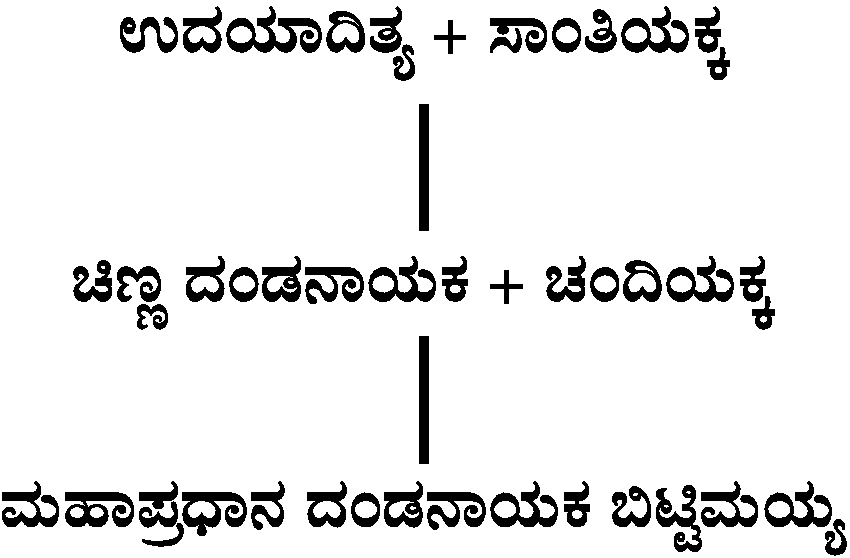
\includegraphics[scale=1.25]{images/chap3/chap3fig17.jpeg}
\end{figure}

\textbf{ಮಹಾಪ್ರಧಾನ ಕಾರೈಕುಡಿ ಕೂತ್ತಾಂಡಿ ದಂಡನಾಯಕ\index{ಮಹಾಪ್ರಧಾನ ಕಾರೈಕುಡಿ ಕೂತ್ತಾಂಡಿ ದಂಡನಾಯಕ} (1157):} ಕಾರೈಕುಡಿ ತಿಲಿಕೂತ್ತಾಂಡಿ ದಂಡನಾಯಕನು ಒಂದನೇ ನರಸಿಂಹನ\index{ಒಂದನೆಯ ನರಸಿಂಹ} ಮಹಾಪ್ರಧಾನ ದಂಡನಾಯಕ, ಸರ್ವಾಧಿಕಾರಿ, ಸೇನಾಧಿಪತಿ ಆಗಿದ್ದನು.\endnote{ ಎಕ 6 ಪಾಂಪು 88 ತೊಣ್ಣೂರು 1157

ಅದೇ, ಪಾಂಪು 98 ತೊಣ್ಣೂರು 12ನೇ ಶ.} ಈತನು ಯಾದವ\-ನಾರಾಯಣ ಚತುರ್ವೇದಿ ಮಂಗಲವಾದ ತೊಂಡನೂರಿನ ಮಧ್ಯಭಾಗದಲ್ಲಿ “ಕಾರಿಕುಡಿ ತಿಲ್ಲೆಕೂತ್ತ ವಿಣ್ನಘರಂ\index{ತಿಲ್ಲೈಕೂತ್ತ ವಿಣ್ನಘರ್ (ವಿಣ್ನಘರ್, ತಿಲ್ಲೆಕೂತ್ತ ವಿಣ್ಣಗರ್)}” ಮಾಡಿಸಿ ಅಲ್ಲಿ “ಶ‍್ರೀಲಕುಮಿ, ಶ‍್ರೀಭೂಮಿ ಸಹಿತವಾಗಿ ವಿತ್ತಿರುಂದ(ವಿರ್ರಿರುಂದ) ಪೆರುಮಾಳೆ” ದೇವರ ತಿರುಪ್ರತಿಷ್ಠೆಯನ್ನು ಮಾಡಿಸಿ ಆ ದೇವರಿಗೆ ಅನೇಕ ಗ್ರಾಮಗಳನ್ನು ಪ್ರಭುಗಾವುಂಡಗಳ ಸಮ್ಮುಖದಲ್ಲಿ ದತ್ತಿಯಾಗಿ ಬಿಟ್ಟನು. ಈತನು ಕಾರೈಕುಡಿಯ ಉಲಗಾಮುಂಡನ ಮಗನೆಂದು ತಿಳಿದುಬರುತ್ತದೆ.\endnote{ ಎಕ 6 ಪಾಂಪು 94 ತೊಣ್ಣೂರು 12 ನೇ ಶ.} ಯಾದವನಾರಾಯಣ ಚತುರ್ವೇದಿ ಮಂಗಲದ\index{ಯಾದವನಾರಾಯಣ ಚತುರ್ವೇದಿ ಮಂಗಲ} ಅಶೇಷ ಮಹಾಜನ\-ಗಳಿಂದ\index{ಅಶೇಷ ಮಹಾಜನಗಳು} ಭೂಮಿಯನ್ನು, ಮಾವಿನಬನವನ್ನು\index{ಮಾವಿನ ಬನ} ಖರೀದಿಸಿ ದತ್ತಿಯಾಗಿ ಈ ದೇವಾಲಯಕ್ಕೆ ದತ್ತಿ ಬಿಟ್ಟನು.\endnote{ ಎಕ 6 ಪಾಂಪು 88 ತೊಣ್ಣೂರು 1157} ಬಹುಶಃ ವೀರನರಸಿಂಹನ ಕಾಲದಲ್ಲಿ, ಇದೇ ಕಾರಿಕುಡಿ ಕೂತ್ತಾನ್​, ಎಂದರೆ ಕಾರೈಕುಡಿ ಕೂತ್ತಾಂಡಿ ದಂಡನಾಯಕನು ರಾಜರಾಜಪುರ\-ದಲ್ಲಿರುವಾಗ, ವಾಗೀಶ್ವರಮಂಗಲದ (ಸೋಮನಹಳ್ಳಿ)\index{ವಾಗೀಶ್ವರಮಂಗಲ (ಸೋಮನಹಳ್ಳಿ)} ಮೂರು ದೇವರುಗಳ ಭೂಮಿಯನ್ನು ನಕರಗಳ\index{ನಕರ (ನಖರ)} ಸಮ್ಮುಖದಲ್ಲಿ ಖರೀದಿಸಿ ದತ್ತಿಯಾಗಿ ಬಿಟ್ಟಿರುತ್ತಾನೆ. ಅದನ್ನು ವೀರಬಲ್ಲಾಳನ ಕಾಲದಲ್ಲಿ ಮತ್ತೆ ನಖರಗಳೆಲ್ಲರೂ\index{ನಕರ (ನಖರ)} ಸೇರಿ ಪುನಃ ದತ್ತಿ ನೀಡಿದಂತೆ ತಿಳಿದುಬರುತ್ತದೆ.\endnote{ ಎಕ 7 ಮವ 109 ಸೋಮನಹಳ್ಳಿ 12ನೇ ಶ.}

\textbf{ಮಹಾಪ್ರಧಾನ ದಂಡನಾಯಕ ಅಚ್ಯುತಿಮಯ್ಯ\index{ಅಚ್ಯುತಿಮಯ್ಯ} ಮತ್ತು ವೀರಯ್ಯ\index{ವೀರಯ್ಯ} (1186\general{\enginline{-}}89):} ಶ‍್ರೀಮನ್ಮಹಾಪ್ರಧಾನ ಸರ್ವಾಧಿಕಾರಿ ಸೇನಾಪತಿ\index{ಸರ್ವಾಧಿಕಾರಿ ಸೇನಾಪತಿ} ಮಹಾಪಸಾಯ್ತ ದಂಡನಾಯಕ ಅಚ್ಯುತಿಮಯ್ಯ ಮತ್ತು ದಂಡನಾಯಕ ವೀರಯ್ಯ ಇವರುಗಳು ಇಮ್ಮಡಿ ಬಲ್ಲಾಳನ ಕಾಲದಲ್ಲಿ ಯಾದವಗಿರಿ (ಮೇಲಕೋಟೆ)\index{ಯಾದವಗಿರಿ (ಮೇಲಕೋಟೆ)} ಕೋಟೆಯ ರಕ್ಷಾಪಾಳಕರಾಗಿದ್ದರು. ಇವರ ಮಕ್ಕಳು ನೀಲಯ್ಯ ಮತ್ತು ಚಾಮಯ್ಯ ಇವರು ಕೋಟೆಯ ಹೊಲಗಾಹು ವೃತ್ತಿಯನ್ನು ಆಳುತ್ತಿದ್ದರೆಂದು, ಇವರು ತೊಂಡನೂರು ಅಗ್ರಹಾರದ\index{ತೊಂಡನೂರು ಅಗ್ರಹಾರ} ಗಡಿಯ ನಖರೇಶ್ವರ\index{ನಖರೇಶ್ವರ} ದೇವರಿಗೆ ದತ್ತಿ ಬಿಟ್ಟರೆಂದು ತಿಳಿದುಬರುತ್ತದೆ.\endnote{ ಎಕ 6 ಪಾಂಪು 74 ತೊಣ್ಣೂರು 1189}\textbf{ವೀರಬಲ್ಲಾಳನ ಮಹಾಪ್ರಧಾನನೂ ಸರ್ವಾಧಿಕಾರಿಯೂ\index{ಸರ್ವಾಧಿಕಾರಿ}, ಶ‍್ರೀಕರಣಾಗ್ರಗಣ್ಯನೂ\index{ಶ‍್ರೀಕರಣಾಗ್ರಗಣ್ಯ}, ಸರ್ವಾಧ್ಯಕ್ಷನೂ\index{ಸರ್ವಾಧ್ಯಕ್ಷ}, ಭಾರದ್ವಾಜಗೋತ್ರದವನು, ವೇದಶಾಸ್ತ್ರ ವಿನೋದನೂ ಆದ, ವೀರಯ್ಯದಂಡನಾಯಕನ ಮತ್ತು ಅವನ ತಮ್ಮನಾದ ಅಚ್ಯುತ ಅಥವಾ ಅಚ್ಯುತದೇವನ }ಪ್ರಸ್ತಾಪ ಬೇಲೂರು ತಾಲ್ಲೂಕು ವೀರದೇವನಹಳ್ಳಿಯ ಕ್ರಿ.ಶ.1186ರ ಶಾಸನ\-ದಲ್ಲಿದೆ.\endnote{ ಎಕ 9 ಬೇಲೂರು 438 ವೀರದೇವನಹಳ್ಳಿ 1186} ರುದ್ರದೇವನ ಹೆಂಡತಿ ಗಂಗಾದೇವಿ. ಇವರ ಮಗ ಅಚ್ಯುತದೇವನನ್ನು \textbf{“ಸಮರಮುಖಲಸದ್​ ರುದ್ರದೇವಾತ್ಮಜಂ, ಯದುರಾಜನ ಮಂತ್ರಿ”} ಎಂದು ವರ್ಣಿಸಲಾಗಿದೆ. ಅಚ್ಯುತದೇವನು ದಂಡನಾಯಕನೂ ಮಂತ್ರಿಯೂ ಆಗಿದ್ದು, ಯಾವುದೋ ಯುದ್ಧದಲ್ಲಿ ಮಡಿದಿರಬಹುದು. ಅವನ ಸಹೋದರ ವೀರಯ್ಯನು ಇವನ ಸ್ಮರಣಾರ್ಥವಾಗಿ ಅಚ್ಯುತಸಮುದ್ರ ಕೆರೆಯನ್ನು ಕಟ್ಟಿಸಿದ್ದಾನೆ. ವೀರಯ್ಯದಂಡನಾಯಕನು ತನ್ನ ನಿಜಸ್ವಾಮಿ ವೀರಬಲ್ಲಾಳ ದೇವನ ಅಭ್ಯುದಯಾರ್ಥ ವೀರಬಲ್ಲಾಳಪುರವನ್ನು\index{ವೀರಬಲ್ಲಾಳಪುರ} ನಿರ್ಮಿಸಿ, ಅಲ್ಲಿ ರುದ್ರಸಮುದ್ರ, ಗಂಗಾಸಮುದ್ರ ಮತ್ತು ಅಚ್ಯುತಸಮುದ್ರ ಎಂಬ ಕೆರೆಗಳನ್ನು ಕಟ್ಟಿಸಿದನು. ಹಾಗೂ ವೀರನಾರಾಯಣದೇವರ ಪ್ರತಿಷ್ಠೆಯನ್ನು ಮಾಡಿ ಅನೇಕ ದತ್ತಿಗಳನ್ನು ಬಿಟ್ಟನೆಂಬುದು ವೀರದೇವನಹಳ್ಳಿ ಶಾಸನದಿಂದ ತಿಳಿದುಬರುತ್ತದೆ. ತೊಣ್ಣೂರು ಶಾಸನದಲ್ಲಿ ವೀರಯ್ಯನನ್ನು ಕೇವಲ ದಂಡನಾಯಕನೆಂದು ಹೇಳಿದ್ದು, ಇದೇ ಕಾಲದ ವೀರನಹಳ್ಳಿ ಶಾಸನದಲ್ಲಿ ಮಹಾಪ್ರಧಾನನೂ ಸರ್ವಾಧಿಕಾರಿ ಶ‍್ರೀಕರಣಾಗ್ರಗಣ್ಯ ಸರ್ವಾಧ್ಯಕ್ಷನೆಂದು ಹೇಳಿದೆ. ದಂಡನಾಯಕನ ಹುದ್ದೆಯಿಂದ ಇವನು ಮಹಾಪ್ರಧಾನ ಸರ್ವಾಧಿಕಾರಿ ಹುದ್ದೆಗೇರಿರುವುದು ಕಂಡುಬರುತ್ತದೆ. ಇವರ ವಂಶಾವಳಿ ಈ ಕೆಳಗಿನಂತಿದೆ.

\begin{figure}[!h]
\includegraphics[scale=.4]{images/chap3/chap3fig18.jpeg}
\end{figure}

\textbf{ಮಹಾಪ್ರಧಾನ ಸರ್ವಾಧಿಕಾರಿ\index{ಮಹಾಪ್ರಧಾನ ಸರ್ವಾಧಿಕಾರಿ} ಸೇನಾಪತಿ\index{ಸೇನಾಪತಿ} ಹಿರಿಯದಂಡನಾಯಕ ಲಕುಮಯ್ಯ\index{ಲಕುಮಯ್ಯ} (1180\general{\enginline{-}}81):} ಇಮ್ಮಡಿ ಬಲ್ಲಾಳನ ಕಾಲದಲ್ಲಿ \textbf{ಲಕುಮಯ್ಯನು ಶ‍್ರೀಮನ್​ ಮಹಾಪ್ರಧಾನ, ಸರ್ವಾಧಿಕಾರಿ, ಸೇನಾಪತಿ, ಮಹಾಪಸಾಯ್ತ, ಬಾಹತ್ತರ ನಿಯೋಗಾಧಿಪತಿ\index{ಬಾಹತ್ತರ ನಿಯೋಗಾಧಿಪತಿ}, ಹಿರಿಯ ದಂಡನಾಯಕನಾಗಿದ್ದನು.} ಈತನು ಇಂದಿನ ಮಳವಳ್ಳಿ ತಾಲ್ಲೂಕು ಸರಗೂರ ಅಮೃತೇಶ್ವರ ದೇವರಿಗೆ ದತ್ತಿಯನ್ನು ಬಿಟ್ಟನು.\endnote{ ಎಕ 7 ಮವ 116 ಸರಗೂರು1180-81} ಈತನು ಒಂದನೇ ನರಸಿಂಹನ ಕಾಲದಲ್ಲೂ ಕೂಡಾ ದಂಡನಾಯಕನಾಗಿದ್ದನು. ಮಹಾಪ್ರಧಾನ ದಂಡನಾಯಕ ವಿಷ್ಣುದಂಡಾಧೀಶ ಅಥವಾ ಬಿಟ್ಟಿಮಯ್ಯನು ಧರ್ಮಾಪುರವನ್ನು\index{ಧರ್ಮಾಪುರ} ಅಗ್ರಹಾರವನ್ನಾಗಿ ಮಾಡಿ ಅಲ್ಲಿನ ಕೇಶವ ದೇವರಿಗೆ ದತ್ತಿಯನ್ನು ಬಿಟ್ಟಾಗ ಅವನ ಜೊತೆ ಹಿರಿಯಭಂಡಾರಿ ಹುಳ್ಳ, ಪಸಾಯ್ತ ಸುರಿಗೆ ನಾಗಯ್ಯ, ಲಕುಮಯ್ಯ ಇವರುಗಳೂ ಇದ್ದರೆಂದು ಹೇಳಿದೆ. ಈತನು ನರಸಿಂಹ ಕಾಲದಲ್ಲಿ ದಂಡಾಧೀಶನಾಗಿದ್ದು ನಂತರ ಮಹಾಪ್ರಧಾನನ ಹುದ್ದೆಗೆ ಏರಿರಬಹುದೆಂದು ಹೇಳಬಹುದು.\endnote{ ಎಕ 4 ಹುಣಸೂರು 24 ಧರ್ಮಾಪುರ 1162}

\textbf{ಮಹಾಪ್ರಧಾನ ಮಾಧವ ದಂಡನಾಯಕ\index{ಮಹಾಪ್ರಧಾನ ಮಾಧವ ದಂಡನಾಯಕ} (1178): }ಮಾಧವನು ಇಮ್ಮಡಿ ಬಲ್ಲಾಳನ ಮಹಾಪ್ರಧಾನ ದಂಡನಾಯಕ\-ನಾಗಿದ್ದನೆಂದು ಹಟ್ಟಣದ ಶಾಸನದಿಂದ ತಿಳಿದುಬರುತ್ತದೆ. ಹೊಯ್ಸಳ ಪಟ್ಟಣಸ್ವಾಮಿ ಸೋಮಿಸೆಟ್ಟಿಯು ಪಟ್ಟಣದಲ್ಲಿ ಪಾರ್ಶ್ವಜಿನಗೃಹವನ್ನು ಮಾಡಿಸಿದಾಗ ಅದಕ್ಕೆ ಮಹಾಪ್ರಧಾನ ಮಾಧವ ದಂಡನಾಯಕರ ಬೆಸದಿಂದ, ಬಹಿತ್ರದ ನಾರಣವೆರ್ಗಡೆ ಕೆಲವು ಸುಂಕಗಳನ್ನು ದತ್ತಿಯಾಗಿ ಬಿಡುತ್ತಾನೆ.\endnote{ ಎಕ 7 ನಾಮಂ 118 ಹಟ್ಟಣ 1178} ಇದರಿಂದ ಸುಂಕದ ಮೇಲಿನ ಅಧಿಕಾರವೂ ಮಹಾಪ್ರಧಾನರಿಗೆ ಇತ್ತು ಎಂಬುದು ತಿಳಿದುಬರುತ್ತದೆ.

\textbf{ಮಹಾಪ್ರಧಾನ ದಂಡನಾಯಕ\index{ಮಹಾಪ್ರಧಾನ ದಂಡನಾಯಕ} ಅಡ್ಡಾಯ್ದದ ಹರಿಹರ\index{ಅಡ್ಡಾಯಿದದ ಹರಿಹರ ದಂಡನಾಯಕ}(1234):} ತೆನದಂಕಾನ್ವಯ ವಂಶದ, ಅಡ್ಡಾಯ್ದದ ಹರಿಹರ ದಂಡನಾಯಕನು ಇಮ್ಮಡಿ ನರಸಿಂಹ ಮತ್ತು ಸೋಮೇಶ್ವರ ಇವರ ಕಾಲದಲ್ಲಿ \textbf{ಅನ್ವಯಾಗತ ಮಹಾಪ್ರಧಾನ\index{ಅನ್ವಯಾಗತ ಮಹಾಪ್ರಧಾನ} ದಂಡನಾಯಕನೂ, ಮಂತ್ರಿಯೂ ಆಗಿದ್ದನು}. ಬಸುರಿವಾಳು ಅಂದರೆ ಇಂದಿನ ಬಸರಾಳು ಇವನ ಊರಾಗಿರಬಹುದು. ಸೂಕ್ತಿಸುಧಾರ್ಣವದ ಕರ್ತೃ ಯೋಗಿಪ್ರವರ ಚಿದಾನಂದ ಮಲ್ಲಿಕಾರ್ಜುನನು ರಚಿಸಿರಬಹುದಾದ ಬಸರಾಳು\index{ಬಸರಾಳು (ಬಸರಿವಾಳ - ಬಸುರುವಾಳು - ಬಸುರಿವಾಳ - ಬಸರುವಾಣ(ಣು))} ಶಾಸನ ಇವನ ವಂಶವೃಕ್ಷವನ್ನು, ಇವನ ಸಾಧನೆ ಸಿದ್ಧಿಗಳನ್ನು ತಿಳಿಸುತ್ತಿದೆ.\endnote{ ಎಕ 7 ಮಂ 29 ಬಸರಾಳು 1234 ಏಪ್ರಿಲ್​ 3} ಅಡ್ಡಾಯುಧ(ಅಢಾಯುಧ) ಎಂದರೆ ಚಿಕ್ಕ ಆಯುಧ ಅಥವಾ ಒಂದು ಬಗೆಯ ಕತ್ತಿ.\endnote{ ಚಿದಾನಂದಮೂರ್ತಿ ಡಾ॥ ಎಂ., ಮಂಥನ, ಸಾಧನೆ, ಸಂಪುಟ 6 ಸಂಚಿಕೆ 1, ಜನವರಿ-ಮಾರ್ಚ್ 1977, ಬೆಂಗಳೂರು ವಿವಿ.}

ತೆನದಂಕಾನ್ವಯದ\index{ತೆನದಂಕಾನ್ವಯ} ಮೇರು ಚಿಕ್ಕಹಡೆವಳ್ಳ. \textbf{ವಿಷ್ಣುವರ್ಧನನು ಇವನಿಗೆ ಪ್ರೀತಿಯಿಂದ ದಿವ್ಯವಾಹನ\index{ದಿವ್ಯವಾಹನ}, ದಂಡಿಗೆ\index{ದಂಡಿಗೆ}, ಅಡಪ\index{ಅಡಪ}, ಪಿಂಛಾತಪತ್ರಾನ್ವಿತಾಸನ\index{ಪಿಂಛಾತಪತ್ರಾನ್ವಿತಾಸನ} (ಮಯೂರಾಸನ), ಈ ರಾಜಚಿಹ್ನೆಗಳನ್ನು ನೀಡಿದನು}. ಇವನ ಹೆಂಡತಿ ನಾಗಲೆ. ಇವರ ಮಗ ಮಲ್ಲೆಯನಾಯಕ. ಮಲ್ಲೆಯನಾಯಕನ ಹೆಂಡತಿ ಗುಜ್ಜಲೆ. ಇವರಿಗೆ ಧರೆ ಅಮ್ಮಮ್ಮ ಎಂದು ಉದ್ಗರಿಸುವಂತೆ, ಅನ್ವಯ ತಿಲಕರಂತೆ ಇದ್ದ \textbf{‘ಸಂಗರಕೆ’ ಸಿಂಗೆಯನಾಯಕ, ‘ಉದಾರವಾರಿನಿಧಿ ಮಾರೆಯನಾಯಕ’, ‘ಧ್ವಜಿನೀಪತಿ\index{ಧ್ವಜಿನೀಪತಿ} ಹರಿಹರ’} ಎಂಬ ಮೂವರು ಮಕ್ಕಳು.

ಧ್ವಜಿನೀಪತಿಯಾದ ಹರಿಹರ ಅಂದರೆ, ಹರಿಹರ ದಂಡನಾಯಕನು, ಹೊಯ್ಸಳರ ಎರಡನೆಯ ನರಸಿಂಹನಲ್ಲಿ ದಂಡನಾಥ\-ನಾಗಿ ಸೇರಿ, ಸೋಮೇಶ್ವರನ ಕಾಲಕ್ಕೆ ಮಹಾಪ್ರಧಾನ ದಂಡನಾಯಕನೆನಿಸಿದನು. \textbf{ನರಸಿಂಹೋರ್ವ್ವೀಶನ ಅಡ್ಡಾಯ್ದದ ಹರಿಹರ ದಂಡನಾಥನು ಕನ್ಯಾದಾನ, ಭೂದಾನ, ಗೋದಾನ, ದೇವತಾಮಂದಿರ, ವಿದ್ಯಾದಾನಗಳಿಂದ ಅಗ್ರಗಣ್ಯನೆನಿಸಿ. ಸೇವುಣರ ಸೈನ್ಯವನ್ನು ಹೊಡೆದಟ್ಟಿದನು. }

\begin{verse}
\textbf{ಕಡುಪಿಂ ಮುತ್ತಿದ ವೀರಸೇವುಣರ ಸೈನ್ಯಾನೀಕಮಂ ಪೊಕ್ಕುಮೆ} \\\textbf{ಯ್ದೆಡೆ ಕೊಂದಿಕ್ಕಿದನೊಕ್ಕಿಲಿಕ್ಕಿ ತುಳಿದಂ ಬೆಂನಟ್ಟಿದಂ ಮುಟ್ಟಿದಂ} \\\textbf{ಪಿಡಿದಂ ಸಾಲೆ ತುರಂಗಮಂ ಹರಿಹರಂ ತನ್ನೊಂದೆ ಜಾತ್ಯಶ್ವದಿಂ} \\\textbf{ಗಡ ವಿಶ್ವಾವನಿ ಮೆಚ್ಚೆ ಮಂತ್ರಿತಿಳಕಂ ವಿದ್ವಿಷ್ಟ ವಿದ್ರಾವಣಂ }
\end{verse}

ಸೋಮೇಶ್ವರನ\index{ಸೋಮೇಶ್ವರ} ಕಾಲದಲ್ಲಿ ಸೇವುಣ ಕೃಷ್ಣನು, ತುಂಗಭದ್ರೆಯನ್ನು ದಾಟಿ ಚಿತ್ರದುರ್ಗ ಪರಿಸರಕ್ಕೆ ಬಂದಿದ್ದ ವಿಚಾರವನ್ನು ಇತಿಹಾಸಕಾರರು ಗುರುತಿಸಿದ್ದಾರೆ.\endnote{ ಸೂರ್ಯನಾಥಕಾಮತ್​ ಡಾ॥, ಕರ್ನಾಟಕದ ಸಂಕ್ಷಿಪ್ತ ಇತಿಹಾಸ, ಪುಟ 94} ಈ ಯುದ್ಧದಲ್ಲಿ ಸೇವುಣರ ಉರವಣೆಯನ್ನು ಒತ್ತರಿಸಿದವನು ದಂಡನಾಯಕ ಹರಿಹರ.\endnote{ ಕೃಷ್ಣರಾವ್​ ಪ್ರೊ॥ ಎಂ.ವಿ., ಕರ್ನಾಟಕ ಇತಿಹಾಸದರ್ಶನ, ಪುಟ 266-67} ಬಸರಾಳು ಮಲ್ಲಿಕಾರ್ಜುನ ದೇವಾಲಯದ\index{ಮಲ್ಲಿಕಾರ್ಜುನ ದೇವಾಲಯ} ಭಿತ್ತಿಯ ಶಿಲ್ಪಗಳಲ್ಲಿ, ಹರಿಹರ ದಂಡನಾಯಕನು ಸೇವುಣರೊಡನೆ ನಡೆಸಿದ ತುರಗ ಪದಾತಿ ಯುದ್ಧದ ಶಿಲ್ಪಗಳಿವೆ. ಹರಿಹರ ದಂಡನಾಯಕನು ಜನನಿಯ ಹೆಸರಿನಿಂದ ಕೆರೆ, ಜನಕನ ಹೆಸರಿಂದ\break ದೇವತಾಗೃಹ(ಮಲ್ಲಿಕಾರ್ಜುನ ದೇವಾಲಯ)ವನ್ನು, ಬಸುರಿವಾಳದೊಳು\index{ಬಸುರಿವಾಳ} ಸುಪ್ರತಿಷ್ಠೆಯಂ ಮಾಡಿಸಿ, ದೇವರ ಶ‍್ರೀಕಾರ್ಯಕ್ಕೆ ನಾರಸಿಂಹದೇವರಸ ಕೈಯಲು ಧಾರೆಯಂ ಪಡೆದು, ಬೆಳೆಯನ ಹಳ್ಳಿಯನ್ನು, ಗದ್ದೆ ಬೆದ್ದಲುಗಳನ್ನು ದತ್ತಿಯಾಗಿ ಬಿಡುತ್ತಾನೆ. ಕ್ರಿ.ಶ.1237ರ ಹೊತ್ತಿಗೆ ಹರಿಹರ ದಂಡನಾಯಕನು ಮಹಾಪ್ರಧಾನ ಪದವಿಯ ಜೊತೆಗೆ ಪರಮವಿಶ್ವಾಸಿ, ಬಾಹತ್ತರ\break ನಿಯೋಗಾಧಿಪತಿ\index{ಬಾಹತ್ತರ ನಿಯೋಗಾಧಿಪತಿ} ಪದವಿಗಳನ್ನು ಪಡೆದು, ನಿಯೋಗದುರಂಧರ, ಸಾಲಮಂನೆಯ ಬೇಂಟೆಕಾರ\index{ಸಾಲಮಂನೆಯ ಬೇಂಟೆಕಾರ}, \textbf{ನಾಲ್ವತ್ತು ನಾಯಕರ ಗಂಡ\index{ನಾಲ್ವತ್ತು ನಾಯಕರ ಗಂಡ}} ಎಂಬ ಬಿರುದುಗಳನ್ನು ಪಡೆದನು.\endnote{ ಎಕ 7 ಮಂ 30 ಬಸರಾಳು 1237 ಅಕ್ಟೋಬರ್​ 22} ದಂಡನಾಯಕರಿಗೆ ಅವರ ಯೋಗ್ಯತೆಯ ಮೇಲೆ ಪದೋನ್ನತಿ ದೊರೆಯುತ್ತಿತ್ತು, ಇವರ ಕೈಕೆಳಗೆ, (ಸೇನಾ) ನಾಯಕರುಗಳು ಇರುತ್ತಿದ್ದರು ಎಂಬುದು ಇದರಿಂದ ತಿಳಿದುಬರುತ್ತದೆ.

ಕ್ರಿ.ಶ.1267ರ ಶಾಸನವು ಹರಿಹರ ದಂಡನಾಯಕನನ್ನು ವೀರಸೋಮೇಶ್ವರದೇವನ ಪಾದಪದ್ಮೋಪಜೀವಿಯೆಂದು ಹೇಳಿದೆ. ಬಹುಶಃ ಈ ಹೊತ್ತಿಗೆ ಅವನು ವಯೋವೃದ್ಧನಾಗಿರಬಹುದು. ಹರಿಹರದಂಡನಾಯಕನಿಗೆ ಹರಿಯಣ್ಣ ಮತ್ತು ನಾರಸಿಂಹದೇವ ಎಂಬ ಇಬ್ಬರು ಮಕ್ಕಳು. ಇವರು ಮಲ್ಲಿಕಾರ್ಜುನ ದೇವಾಲಯದ ಸ್ಥಾನಿಕರಾಗಿದ್ದರೆಂದು\index{ಸ್ಥಾನೀಕರು} ತಿಳಿದುಬರುತ್ತದೆ.\endnote{ ಎಕ 7 ಮಂ 31 ಬಸರಾಳು 1267 ಏಪ್ರಿಲ್​ 11.}\break \textbf{ಹರಿಹರನು ಅನ್ವಯಾಗತ ಪ್ರಧಾನಿಯಾಗಿದ್ದರೂ ಅವನ ಮಕ್ಕಳು ಪ್ರಧಾನಿಗಳಾಗಲಿಲ್ಲ, ಅಧಿಕಾರ ಸ್ಥಾನ ಪಡೆಯಲಿಲ್ಲ. ಇದೂ ಕೂಡಾ ಪ್ರಧಾನಿ ಅಥವಾ ಇತರ ಅಧಿಕಾರಿ ಹುದ್ದೆಗೆ ಅರ್ಹತೆಯೂ ಬಹಳ ಮುಖ್ಯವಾಗಿತ್ತೆಂಬುದನ್ನು ತೋರಿಸುತ್ತದೆ. }ಮೇಲ್ಕಂಡ ಶಾಸನಗಳಿಂದ ತಿಳಿದುಬರುವ ಹರಿಹರದಂಡನಾಯಕನ ವಂಶವೃಕ್ಷ ಈ ಕೆಳಗಿನಂತಿದೆ.
\begin{figure}[H]
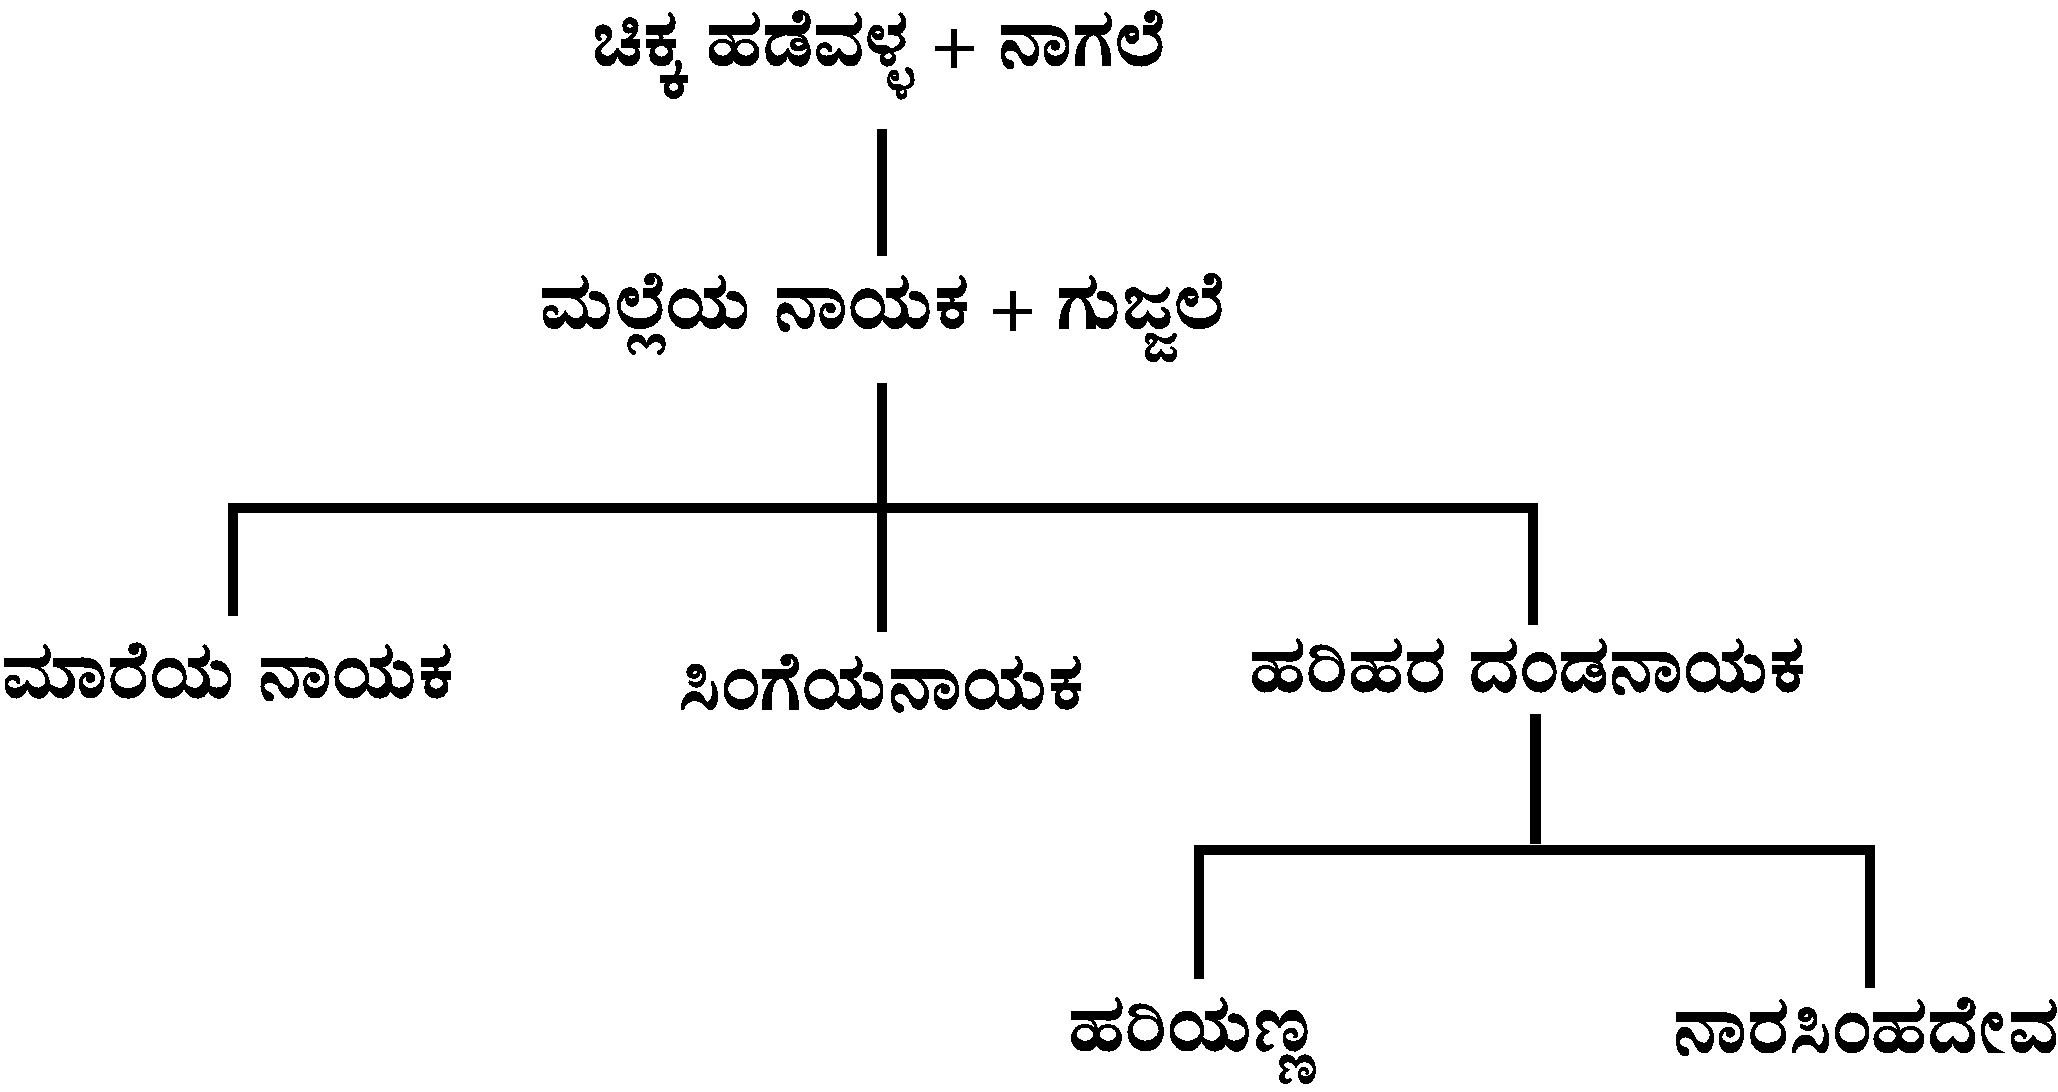
\includegraphics[scale=1.15]{images/chap3/chap3fig19.jpeg}
\end{figure}

\textbf{ಮಂತ್ರಿ, ದಂಡನಾಯಕ, ಮಂಡಲೀಕ ಬೋಗೈಯ್ಯ\index{ಬೋಗೈಯ್ಯ} ಮತ್ತು ಮುರಾರಿ ಮಲ್ಲಯ್ಯ\index{ಮುರಾರಿ ಮಲ್ಲಯ್ಯ}(1236):} ಬೋಗೈಯ್ಯ\break ದಂಡನಾಯಕ ಮತ್ತು ಅವನ ತಮ್ಮ ಮುರಾರಿ ಮಲ್ಲಯ್ಯ ಇವರುಗಳು ಸೋಮೇಶ್ವರನ ಬಳಿ ಮಾಂಡಲೀಕರು ಮತ್ತು ದಂಡನಾಯಕರುಗಳು ಆಗಿದ್ದರು.\endnote{ ಎಕ 6 ಕೃಪೇ 39 ಗೋವಿಂದನಹಳ್ಳಿ 1236}\textbf{ “ದ್ವಾವೇತಾವಥ ಹೊಯ್ಸಲಾಹ್ವಯವತ ಸೋಮೇಶ್ವರ ಕ್ವ್ಮಾಪತೇಃ ಪ್ರಖ್ಯಾತೌ ಭುವಿ ಮಂತ್ರಿಣಾವಭವತಾಂ ಸ್ವೀಯಪ್ರತಾಪೋದಯೌ”} ಎಂದು ಹೇಳಿರುವುದರಿಂದ ಇವರು ಮಂತ್ರಿಗಳೂ ಆಗಿದ್ದರು. ಇವರು \textbf{‘ಕೇತಣವಾಹಿನೀ ಪರಿವೃಢಃ’} ಅಂದರೆ, ಕೇತಣ್ಣ ದಂಡನಾಯಕನ\index{ಕೇತೆಯ (ಕೇತಣ್ಣ-ಕೇತಯ್ಯ-ಕೇತಪ್ಪ) ದಂಡನಾಯಕ (ದಂಣ್ನಾಯಕ)} ಮಕ್ಕಳು. ಕಬ್ಬುಹುನಾಡ\index{ಕಬ್ಬಾಹು-(ಕಬಾಹು-ಕಬ್ಬಹು-ಕಬ್ಬಪ್ಪು ) ಸಾಸಿರ-ನಾಡು-ವಿಷಯ} ತೆಂಗಿನಕಟ್ಟವನ್ನು\index{ತೆಂಗಿನಕಟ್ಟ} (ಇಂದಿನ ತೆಂಗಿನಘಟ್ಟ) ಅದಕ್ಕೆ ಸೇರಿದ ಹನ್ನೊಂದು ಹಳ್ಳಿಗಳ ಸಮೇತ, ಪ್ರಸನ್ನ ಸೋಮನಾಥಪುರವೆಂಬ\index{ಪ್ರಸನ್ನ ಸೋಮನಾಥಪುರವಾದ ತೆಂಗಿನಕಟ್ಟ (ತೆಂಗಿನಘಟ್ಟ)} ಅಗ್ರಹಾರವನ್ನಾಗಿ ಮಾಡಿ ಸೇತುವಿನ ಶ‍್ರೀರಾಮನಾಥದೇವರ ಸನ್ನಿಧಿಯಲ್ಲಿ ಬ್ರಾಹ್ಮಣರಿಗೆ ದತ್ತಿ ಬಿಟ್ಟರು. \textbf{“ಸ್ವಕೀಯೈಕಾದಶಪಲ್ಲಿ ಸಹಿತಂ, ತನ್ನ ಹಳ್ಳಿಗಳೊಡಗೂಡಿದ್ದ”} ಎಂದು ಶಾಸನದಲ್ಲಿ ಹೇಳಿರುವುದರಿಂದ ಇವರು ಕಬ್ಬಾಹು ನಾಡಿನ\index{ಕಬ್ಬಾಹು-(ಕಬಾಹು-ಕಬ್ಬಹು-ಕಬ್ಬಪ್ಪು ) ಸಾಸಿರ-ನಾಡು-ವಿಷಯ} ಮಾಂಡಲಿಕರಾಗಿದ್ದರೆಂದು ಹೇಳ\-ಬಹುದು. ಬೋಗೈಯ್ಯ ದಂಡನಾಯಕನಿಗೂ ಕಳಚುರ್ಯರ ಸೋವಿದೇವನಿಗೂ\index{ಸೋವಿದೇವ} ಯುದ್ಧವಾದ ವಿಚಾರ ಚಿಕ್ಕೊಲೆ ಶಾಸನದಿಂದ ತಿಳಿದು\-ಬರುತ್ತದೆ.\endnote{ ಎಕ 9 ಬೇಲೂರು 501 ಚಿಕ್ಕೊಲೆ 1244} ಸೋಮೇಶ್ವರನು ಕಳಚುರಿ ಸೋವಿದೇವನೊಡನೆ ಹೋರಾಡಿದುದನ್ನು \textbf{“ಶೌರ್ಯದಿಂ ಬೆನ್ನಂ ಪತ್ತಿಸೆ ಸೋವಿದೇವಘಟೆಯಂ ಕೈಕೊಂಡರಾರ್​”} ಎಂದು ಬಸರಾಳು ಶಾಸನವು ವರ್ಣಿಸಿದೆ.\endnote{ ಎಕ 7 ಮಂ 30 ಬಸರಾಳು 1237}

\textbf{ಮಹಾಪ್ರಧಾನ ದಂಡನಾಯಕ\index{ಮಹಾಪ್ರಧಾನ ದಂಡನಾಯಕ} ಸೋಮೆಯ ದಂಡನಾಯಕ\index{ಸೋಮೆಯ ದಂಡನಾಯಕ (ದಣ್ನಾಯಕ)}\general{\enginline{-}}ಮಲ್ಲಿದೇವ\index{ಮಲ್ಲಿದೇವ ದಂಡನಾಯಕ}  \general{\enginline{–}} ಚಿಕ್ಕಕೇತೆಯ \general{\enginline{-}}ಕೇತೆಯ\index{ಚಿಕ್ಕಕೇತೆಯ}\index{ಚಿಕ್ಕಕೇತೆಯ ದಂಡನಾಯಕ}/ಕೇತ ಚಮೂಪತಿ \general{\enginline{–}} ಸಿಂಗೆಯ ದಂಡನಾಯಕರುಗಳು\index{ಸಿಂಗೆಯ ದಂಡನಾಯಕ (ದಂಣ್ನಾಯಕ)} (1269\general{\enginline{-}}1296):} ಸೋಮನು ಮೂರನೆಯ ನರಸಿಂಹನ ಕಾಲದಲ್ಲಿದ್ದ ಅತ್ಯಂತ ಸುಪ್ರಸಿದ್ಧನಾದ ಮಹಾಪ್ರಧಾನ ದಂಡನಾಯಕ. ಸೋಮನಾಥಪುರ\index{ಸೋಮನಾಥಪುರ} ಶಾಸನದಲ್ಲಿ ಈತನನ್ನು ನರಸಿಂಹನ ಪ್ರಿಯಸುತನೆಂದು\index{ಪ್ರಿಯಸುತ} ಕರೆಯಲಾಗಿದೆ. 'ಗಂಡಪೆಂಡಾರ\index{ಗಂಡಪೆಂಡಾರ}' ಎಂಬುದು ಇವನ ಬಿರುದುಗಳಲ್ಲಿ ಒಂದು. ಈತನು ನಾರಸಿಂಹನ ಪರವಾಗಿ ಗಂಡಪೆಂಡಾರವನ್ನು\index{ಗಂಡಪೆಂಡಾರ} ಧರಿಸಿದ್ದರಿಂದ ಇವನನ್ನು ಮನೆಮಗ ಎಂಬ ಅರ್ಥದಲ್ಲಿ ಪ್ರಿಯಸುತನೆಂದು ಕರೆದಿರಬಹುದು. (ಪ್ರಿಯಸುತ\enginline{-}ಹಲ್ಮಿಡಿ ಶಾಸನದ ಪ್ರೇಮಾಲಯಸುತ). ಸೋಮೆಯ ದಂಡನಾಯಕನನ್ನು ವೀರನಾರಸಿಂಹನ ಮೈದುನ ಎಂದು ಹೇಳಿದೆ. ಸೋಮೆಯ ದಂಡನಾಯಕನ ತಂಗಿಯನ್ನೇನಾ\-ದರೂ ವೀರನರಸಿಂಹನು ವರಿಸಿ ವೈವಾಹಿಕ ಸಂಬಂಧ ಬೆಳೆಸಿದ್ದನೋ ತಿಳಿದುಬರುವುದಿಲ್ಲ.\endnote{ ಎಕ 9 ಬೇಲೂರು 418 ಹುಲಿಕೆರೆ 1271} ಹೆಂಮೆಯ ದಂಡನಾಥ\index{ಹೆಂಮೆಯ ದಂಡನಾಥ} ಮತ್ತು ರೇವಲಾದೇವಿಯ\index{ರೇವಲಾದೇವಿ} ಮಗನಾದ ಸೋಮನು, ಸೋಮನಾಥಪುರದಲ್ಲಿ ತನ್ನ ತಂದೆ ತಾಯಿಗಳ ಹೆಸರಿನಲ್ಲಿ ಹೆಂಮೇಶ್ವರದೇವರು ಮತ್ತು ರೇವಲೇಶ್ವರ ದೇವಾಲಯಗಳನ್ನು ಕಟ್ಟಿಸಿ ದತ್ತಿ ಬಿಡುತ್ತಾನೆ.\endnote{ ಎಕ 5 ತಿನಪು 96 ಸೋಮನಾಥಪುರ 1276} ಕೃಷ್ಣರಾಜಪೇಟೆ\break ತಾಲ್ಲೂಕು ಭೈರಾಪುರ\index{ಭೈರಾಪುರ (ಅಗ್ರಹಾರ)} ಶಾಸನದಲ್ಲಿ ರೇವಲಾದೇವಿಯನ್ನು, ರೇಕಾದೇವಿ\index{ರೇಕಾದೇವಿ} ಎಂದು ಕರೆದಿದೆ.\endnote{ ಎಕ 6 ಕೃಪೇ 98 ಭೈರಾಪುರ 1267}

\newpage

ಮಂಡ್ಯ, ಮೈಸೂರು ಮತ್ತು ಹಾಸನ ಜಿಲ್ಲೆಯಲ್ಲಿ ದೊರೆಯುವ ಶಾಸನಗಳು ಸೋಮೆಯ ದಂಡನಾಯಕ ಮತ್ತು ಅವನ ಅಳಿಯನಾದ ಕೇತೆಯ ಅಥವಾ ಚಿಕ್ಕಕೇತೆಯ ದಂಡನಾಯಕ\index{ಚಿಕ್ಕಕೇತೆಯ ದಂಡನಾಯಕ} ಮತ್ತು ಮಲ್ಲಿದೇವ ದಂಡನಾಯಕರ\index{ಮಲ್ಲಿದೇವ ದಂಡನಾಯಕ} ಬಗ್ಗೆ ಪ್ರಮುಖವಾದ ಐತಿಹಾಸಿಕ ಅಂಶಗಳನ್ನು ನೀಡುತ್ತವೆ. ಕ್ರಿ.ಶ.1261ರ ವೈದ್ಯನಾಥಪುರದ ಕೇತೆಯ ದಂಡನಾಯಕನ ಶಾಸನವೇ ಸೋಮದಂಡನಾಯಕನನ್ನು ಕುರಿತು ಜಿಲ್ಲೆಯಲ್ಲಿ ದೊರೆಯವ ಮೊದಲ ಶಾಸನ.\endnote{ ಎಕ 7 ಮ 69 ವೈದ್ಯನಾಥಪುರ 1261} ಈ ಶಾಸನದಲ್ಲಿ ಸೋಮೆಯ ದಂಡನಾಯಕನನ್ನು \textbf{“ಶ‍್ರೀಮನು ಮಹಾಪ್ರಧಾನ ಗಾಯಿಗೋಪಾಳ, ಗಣ್ಡಪೆಣ್ಡಾರ, ಮಣ್ಡಳೀಕಜೂಬು”} ಎಂಬ ಬಿರುದುಗಳಿಂದ ಹೊಗಳಲಾಗಿದೆ. ಇದರಲ್ಲಿ “ಸೋಮೆಯ ದಂಡನಾಯಕರ ಅಳಿಯ ಹಿರಿಯ.......” ಎಂಬಲ್ಲಿ ಮಲ್ಲಿದೇವನ ಹೆಸರು ಅಳಿಸಿಹೋಗಿ ಅವನ ನಂತರ ಇನ್ನೊಬ್ಬ ಅಳಿಯ ಕೇತೆಯ ದಂಡನಾಯಕನ ಹೆಸರು ಬಂದಿದೆ. ಶಾಸನದಲ್ಲಿ ಸೋಮ ದಂಡನಾಯಕನನ್ನು ಮಂತ್ರಿ ಲಲಾಮ ಎಂದು ಹೇಳಿದೆ.

\vskip 2pt

\begin{verse}
\textbf{ಆತನ ಮಂತ್ರಿ ಲಲಾಮಂ} \\\textbf{ನೀತಿಗೆ ಚಾಣಕ್ಯನೆನಿಪ ಸೋಮಂಗಳಿಯಂ } \\\textbf{ಕೇತಚಮೂಪತಿ ಪದಪಿಂ} \\\textbf{ಖ್ಯಾತಿಯ ಮದ್ದೂರ ವೈಜನಾಥಂಗೊಲವಿಂ}
\end{verse}

\vskip 2pt

ಕೇತೆಯ ದಂಡನಾಯಕನು ತನ್ನ ಆಳ್ದನ (ವೀರನಾರಸಿಂಹನನ್ನು) ಬೇಡಿಕೊಂಡು ಕೆಳಲೆನಾಡ ಹೆಬ್ಬಟ್ಟದ ಪಡುವಣ ಬೇಡರಹಳ್ಳಿಯನ್ನು ವೈಜನಾಥದೇವರ ಪಾತ್ರಕ್ಕೆ ದತ್ತಿಯಾಗಿ ಬಿಡುತ್ತಾನೆ.

\vskip 2pt

ಪಿರಿಯಪಟ್ಟದ ಅಗ್ರಹಾರ ಹಿರಿಯ ಸೋಮನಾಥಪುರವಾದ\index{ಪಿರಿಯಪಟ್ಟದ ಅಗ್ರಹಾರ ಹಿರಿಯ ಸೋಮನಾಥಪುರ} ಹರುವನಹಳ್ಳಿಯ ಚೆನ್ನಕೇಶವದೇವರ ನೆಲೆವೃತ್ತಿಗಳ\break ತೋಟಸ್ಥಳಗಳನು, ಮಹಾಪ್ರಧಾನ ಸೋಮೆಯದಂಡನಾಯಕರ ಬಲುಮನುಷ್ಯ ಹೆಗ್ಗಡೆ ಪೆದ್ದಣ್ಣನು ಹೊರಗುತ್ತಿಗೆಯಾಗಿ ನೀಡಿದನು.\endnote{ ಎಕ 10 ಅರಸೀಕೆರೆ 233 ಹಾರನಹಳ್ಳಿ 1265} ಕಲುಕಣಿನಾಡ\index{ಕಲುಕಣಿ (ಕಲಿಕಣಿ-ಕಲ್ಕಣಿ-ಕಲ್ಕುಣಿ-ಕಲುಕರೆ) ನಾಡು}, ಕೆಲ್ಲಂಗೆರೆಯ\index{ಕೆಲ್ಲಂಗೆರೆ (ಕೆಲಗೆರೆ)} (ಇಂದಿನ ನಾಗಮಂಗಲ ತಾಲ್ಲೂಕು ಕೆಳಗೆರೆ) ತ್ರಿಕೂಟರತ್ನತ್ರಯ ಶಾಂತಿನಾಥ ಜಿನಾಲಯಕ್ಕೆ\index{ತ್ರಿಕೂಟ ರತ್ನತ್ರಯ ಶಾಂತಿನಾಥ ಬಸದಿ (ಜಿನಾಲ)} ನಾರಸಿಂಹನು ಅನೇಕ ಹಳ್ಳಿಗಳನ್ನು ದತ್ತಿ ಬಿಡುತ್ತಾನೆ. ಈ ಧರ್ಮವು ಮಹಾಪ್ರಧಾನ ಸೋಮೆಯ ದಂಡನಾಯಕನ ಸಹಾಯದಿಂದ ನಡೆಯುತ್ತದೆಂದು ಶಾಸನದಲ್ಲಿ ಹೇಳಿದೆ.\endnote{ ಎಕ 9 ಬೇಲೂರು 321 ಹಳೇಬೀಡು 1265} ಬಸದಿಗಳನ್ನು ರಕ್ಷಿಸುವ ಹೊಣೆಯನ್ನು ರಾಜನು\break ಸೋಮದಂಡನಾಯಕನಿಗೆ ನೀಡಿದ್ದನೆಂದು ಹೇಳಬಹುದು. ವೀರನಾರಸಿಂಹನ ಮೈದುನ ಸೋಮೆಯ ದಂಡನಾಯಕ, ಸೋಮೆಯ ದಂಡನಾಯಕನ ಮೈದುನ ಬಾಚೆಯ ದಂಡನಾಯಕ\index{ಬಾಚೆಯ ದಂಡನಾಯಕ} ಇವರುಗಳು ಹೊಂಕುಂದದ ಬಸದಿಯು ಜೀರ್ಣವಾಗಿರಲು ಅದರ ಜೀರ್ಣೋದ್ಧಾರ ಮಾಡಿಸಿದರು.\endnote{ ಎಕ 9 ಬೇಲೂರು 418 ಹುಲಿಕೆರೆ 1271} ಸೋಮದಂಡನಾಯಕನು ಶೈವನಾದರೂ, ಪಂಚಲಿಂಗೇಶ್ವರ ದೇವಾಲಯಗಳ ಜೊತೆಗೆ ಶ‍್ರೀವೈಷ್ಣವಸ್ಥಳವಾದ ಕೇಶವ ದೇವಾಲಯವನ್ನು ನಿರ್ಮಿಸಿ, ಜೈನಬಸದಿಗಳನ್ನು ಜೀರ್ಣೋದ್ಧಾರ ಮಾಡಿಸಿ, ಅವುಗಳಿಗೆ ದತ್ತಿಗಳನ್ನು ಬಿಡಿಸಿರುವುದು ಇವನ ಪರಮತ ಸಹಿಷ್ಣತೆಯನ್ನು ತೋರಿಸುತ್ತದೆ.

\vskip 2pt

ಸೋಮ ದಂಡನಾಯಕನು ವಿದ್ಯಾನಿಧಿ ಪ್ರಸನ್ನ ಸೋಮನಾಥಪುರವೆಂಬ\index{ವಿದ್ಯಾನಿಧಿ ಪ್ರಸನ್ನ ಸೋಮನಾಥಪುರ} ಅಗ್ರಹಾರವನ್ನು ಮಾಡಿ ಅಲ್ಲಿ ಪ್ರಸನ್ನ\break ಕೇಶವದೇವರು ಮೊದಲಾಗಿ 70 ದೇವರುಗಳನ್ನು ಪ್ರತಿಷ್ಠೆ ಮಾಡಿ ಅನೇಕ ದತ್ತಿಗಳನ್ನು ಬಿಟ್ಟನು.\endnote{ ಎಕ 5 ತಿನಪು 88 ಸೋಮನಾಥಪುರ 1276} ಸೋಮದಂಡನಾಯಕನ ಸೋದರಳಿಯಂದಿರಾದ ಮಲ್ಲಿದೇವ ಮತ್ತು ಚಿಕ್ಕಕೇತೆಯ ದಂಡನಾಯಕರುಗಳು ಕ್ರಿ.ಶ.1276 ರಲ್ಲಿ ಈ ವೃತ್ತಿಗಳನ್ನು ವಿಭಾಗಿಸಿ ಹಂಚಿಕೆ ಮಾಡಿದರು. ಅದೇ ರೀತಿ ಸೋಮದಂಡನಾಯಕನು ಸೋಮನಾಥಪುರದಲ್ಲಿ ಐದು ಈಶ್ವರ ದೇವಾಲಯಗಳನ್ನು (ಪಂಚಲಿಂಗ) ಕಟ್ಟಿಸಿದನು. ಅವುಗಳಿಗೆ ಸೋಮೆಯ ದಂಡನಾಯಕನೂ ಅವನ ಸೊದರಳಿಯಂದಿರಾದ ಮಲ್ಲಿದೇವ ದಂಡನಾಯಕನು ಮತ್ತು ಚಿಕ್ಕಕೇತಯ ದಂಡನಾಯಕರೂ ದತ್ತಿ ನೀಡಿದರೆಂದು ಅಲ್ಲಿರುವ ಇನ್ನೊಂದು ಶಾಸನದಿಂದ ತಿಳಿದು\-ಬರುತ್ತದೆ.\endnote{ ಎಕ 5 ತಿನಪು 96 ಸೋಮನಾಥಪುರ 1276} ಸೋಮನಾಥಪುರ ಶಾಸನವು \textbf{“ಶ‍್ರೀಮನ್​ ಮಹಾಪ್ರಧಾನಂ ಗಾಯಿಗೋಪಾಳ, ಗಣ್ದಪೆಣ್ಡಾರ, ಮಂಡಳೀಕಜೂಬು\index{ಮಂಡಳಿಕಜೂಬು}, ಉದ್ದಂಡ ಮಂಡಳೀಕರಗಂಡ\index{ಮಂಡಳೀಕರಗಂಡ}, ದಂಡನಾಥ ದೇವೇಂದ್ರ, ಅಸರಿಸ್ವಯಂಭು, ಖಳತ್ರಿಣೇತ್ರ, ಅತಿವಿಷಮ ಹಯಾರೂಢ\general{\break } ಪ್ರೌಢರೇಖಾ ರೇವಂತ, ಪರಬಳಕೃತಾಂತ, ಸ್ವೀಕಾರಸಾರೋದಯ, ಅನ್ನದಾನವಿನೋದ, ಸುವರ್ಣದಾನಶೂರ,\general{\break } ಹೆಂಮೆಯದಂಡನಾಥ\index{ಹೆಂಮೆಯ ದಂಡನಾಥ}, ಪೂರ್ವಾಚಲಮಾರ್ತಾಂಡ, ರೇವಲಾಕಲ್ಪವಲ್ಲಿ\index{ರೇವಲಾದೇವಿ} ಪುಷ್ಪೋತ್​ಗಮನ ಸೋಮಣ್ಣದಂಡನಾಯಕರು\index{ಸೋಮಣ್ಣದಂಡನಾಯಕರು}” }ಎಂದು ಅವನ ಬಿರುದಾವಳಿಗಳನ್ನು ನೀಡಿದೆ. ಈ ಬಿರುದಾವಳಿಗಳನ್ನು ಬಹಳ ಮುಖ್ಯವಾಗಿ ಗಮನಿಸಬೇಕಾಗುತ್ತದೆ. ಸೋಮನ ಅಳಿಯಂದಿರಾದ ಮಹಾಮಂಡಳಿಕ ಮಂನೆಯಜೂಬು ಮಲಿದೇವ ದಂಣಾಯಕರು ಮತ್ತು ಚಿಕ್ಕಕೇತಯ್ಯ ದಂಣ್ನಾಯಕರ ಹೆಸರು ಭೈರೇದೇವರ ಗುಡ್ಡ\index{ಭೈರೇದೇವರ ಗುಡ್ಡ} ಶಾಸನದಲ್ಲಿ ಬಂದಿದೆ.\endnote{ ಎಕ 9 ಬೇಲೂರು 552 ಭೈರೇದೇವರಗುಡ್ಡ 1276} ಗಾಯಿಗೋವಳ ಗಂಡಪೆಂಡಾರ\index{ಗಂಡಪೆಂಡಾರ} ಮಂಡಳಿಕಜೂಬು\index{ಮಂಡಳಿಕಜೂಬು} ಕುಮಾರ ಮಲ್ಲಿದೇವ ದಂಡನಾಯಕನು\index{ಕುಮಾರ ಮಲ್ಲಿದೇವ ದಂಡನಾಯಕ} ನಾಗೇಶ್ವರ ದೇವಾಲಯವನ್ನು\index{ನಾಗೇಶ್ವರ ದೇವಾಲಯ} ಕಟ್ಟಿಸುತ್ತಾನೆ. ಈ ಶಾಸನದಲ್ಲಿ ಇವನನ್ನು ನರಸಿಂಹದೇವರ ಕುಮಾರ ಎಂದು ಕರೆದಿದೆ. ಕುಮಾರ ಎಂದರೆ ಮನೆಯಮಗ ಎಂದು ಹೇಳಬಹುದು.\endnote{ ಎಕ 9 ಬೇಲೂರು 422 ಗೋಣಿಸೋಮನಹಳ್ಳಿ 1273} ಈತನು ಸೋಮೆಯ ದಂಡನಾಯಕನ ಅಳಿಯ ಮಲ್ಲಿದೇವ ದಂಡನಾಯಕನೇ ಆಗಿದ್ದಾನೆ. ಚಿಕ್ಕಕೇತೆಯ\index{ಚಿಕ್ಕಕೇತೆಯ} ಇನ್ನೊಬ್ಬ ಅಳಿಯ, ಸೋಮೆಯ ದಂಡನಾಯಕರ ಸೋದರಳಿಯ ಮಾರೂರ ಚಿಕಕೇತಯ ದಂಡನಾಯಕರು\index{ಮಾರೂರ ಚಿಕಕೇತಯ ದಂಡನಾಯಕ} ಎಂದು ಸೋಮನಾಥಪುರ ಶಾಸನದಲ್ಲಿ ಹೇಳಿದೆ.\endnote{ ಎಕ 9 ತಿನಪು 88 ಸೋಮನಾಥಪುರ 1276} ಇದು ಮಾಗಡಿ ಸಮೀಪದ ಮರೂರು ಇರಬಹುದೇ ಎಂದು ಊಹಿಸಬಹುದು.

\vskip 2pt

ಸೋಮೆಯ ದಂಡನಾಯಕನಿಗೆ ಕುಮಾರ ವೀರ ಚಿಕ್ಕಕೇತೆಯ ದಂಡನಾಯಕ\index{ಕುಮಾರ ವೀರ ಚಿಕ್ಕಕೇತೆಯ ದಂಡನಾಯಕ} ಮತ್ತು ಸಿಂಗಪ್ಪ ಅಥವಾ ಸಿಂಗೆಯ ದಂಡನಾಯಕ\index{ಸಿಂಗೆಯ ದಂಡನಾಯಕ (ದಂಣ್ನಾಯಕ)} ಎಂಬ ಇಬ್ಬರು ಮಕ್ಕಳಿದ್ದರು. ಸೇವುಣಾಧಿಪ ರಾಮದೇವನ\index{ಸೇವುಣಾಧಿಪ ರಾಮದೇವ} ಸೇನಾಧಿಪತಿ, ಸಾಳುವತಿಕ್ಕಮನ\index{ಸಾಳುವತಿಕ್ಕಮ} ಸೇನೆಯು ಬೆಳವಡಿಯಲಿ ಬಂದು ಬೀಡುಬಿಟ್ಟಿದ್ದಾಗ ಸೋಮೆಯ ದಂಡನಾಯಕನ ಮಗ ಕುಮಾರ ವೀರ ಚಿಕ್ಕಕೇತೆಯ್ಯನಾಯಕನು (ಚಮೂಧರ ಚಿಕ್ಕಕೇತಣ್ಣ), ಅವನ ಮಗ ಅಂಕೆಯನಾಯಕನು ಸಮಗ್ರಬಲದ ಜೊತೆಗೆ ಹೋಗಿ, ನಾಲ್ದೆಸೆಗೆ ಕವಿದಿದ್ದ, ಹರಿಪಾಲನ ನೇತೃತ್ವದಲ್ಲಿ ಬಂದಿದ್ದ ಸೇವುಣರ ಸೈನ್ಯವನ್ನು ದೆಸೆ ಬಲಿಗೆಯ್ದರಂತೆ. ಹೊಯ್ಸಳ ಸೇನೆಯು ಸಾಳುವ ತಿಕ್ಕಮನನ್ನು ಬೆಳವಾಡಿಯಲ್ಲಿ ಬೀಡುಬಿಡಲು ಆಸ್ಪದ ನೀಡದೆ, ಅಟ್ಟುಣ್ಣಲೀಯದೆ ದುಮ್ಮೆವರೆಗೆ ಓಡಿಸಿಕೊಂಡು ಹೋಯಿತಂತೆ.\endnote{ ಎಕ 9 ಬೇಲೂರು 431 ಕಟ್ಟೇಸೋಮನಹಳ್ಳಿ 1276} ಈ ಶಾಸನದಲ್ಲಿ ಕುಮಾರ ವೀರಚಿಕ್ಕಕೇತಯ್ಯ ಎಂದು ಹೇಳಿರುವುದರಿಂದ ಈತನು ಸೋಮೆಯದಂಡನಾಯಕನ ಮಗನಿರಬಹುದು. ಇನ್ನೊಬ್ಬ ಚಿಕ್ಕಕೇತಯ್ಯ ದಂಡನಾಯಕನನ್ನು ಸೋಮನ ಅಳಿಯ ಎಂದೇ ಶಾಸನಗಳು ವರ್ಣಿಸಿವೆ.

\vskip 2pt

ಇದೇ ಘಟನೆಯನ್ನು ವಿವರಿಸುವ ಇನ್ನೊಂದು ಶಾಸನವೂ ಇಲ್ಲೇ ಇದೆ. ವೀರನಾರಸಿಂಹದೇವರಸರ ರಾಜಧಾನಿ ದೋರಸಮುದ್ರವನ್ನು ಮುತ್ತಲು ಸೇವುಣದಳದ ಮುಖ್ಯಸ್ಥ ಸಾಳುವ ತಿಕ್ಕಮ, ಜೈದೇವ ಮತ್ತು ಹರಿಪಾಳಯ್ಯ ಇವರುಗಳು ಗುಣಗನೆಯಿಂದ ನಡೆದುಬಂದು (ಬೆಳವಡಿಯಲ್ಲಿ) ಬೀಡುಬಿಟ್ಟಲ್ಲಿ, ವೀರನರಸಿಂಹರಾಯರ ಮಗ (ಪ್ರಿಯಸುತ)\break ಗಾಯಿಗೋಪಾಳ, ಗಂಡಪೆಂಡಾರ, ಪಡೆಮೆಚ್ಚೆಗಂಡ ಶ‍್ರೀಮನ್​ಮಹಾಪ್ರಧಾನ ಚಿಕ್ಕಕೇತೆಯ ದಂಡನಾಯಕರ ಬೆಸದಿಂದ ಮಂಡಳಿಕ ಗಂಧವಾರಣ\index{ಮಂಡಳಿಕ ಗಂಧವಾರಣ} ನೊಬೆಯ ಗುಲ್ಲಯ್ಯನು\index{ನೊಬೆಯ ಗುಲ್ಲಯ್ಯ}, ಸೇವುಣಸೇನೆಯನ್ನು ಬೆಳವಡಿಯಿಂದ ದುಮ್ಮೆತನಕ ಅಟ್ಟಾಡಿಸಿಕೊಂಡು ಹೋಗಿ, ಸಾಳುವನ ಮೊಗವನ್ನು ಕೆಡಿಸಿ, ಹೋರಾಡಿ, ವೀರಸಿದ್ಧಿವೆರಸು ಸುರಲೋಕಪ್ರಾಪ್ತನಾದನು.\endnote{ ಎಕ 9 ಬೇಲೂರು 430 ಕಟ್ಟೆಸೋಮನಹಳ್ಳಿ 1276} ಈ ಯುದ್ಧದಲ್ಲಿ ಬಹುಶಃ ವೀರಚಿಕ್ಕಕೇತೆಯ ದಂಡನಾಯಕನೂ ಮಡಿದಿರಬಹುದೆಂದು ಎಪಿಗ್ರಾಫಿಯಾ ಸಂಪಾದಕರು ಅಭಿಪ್ರಾಯ ಪಟ್ಟಿದ್ದಾರೆ. ಆದರೆ ಇಲ್ಲೇ ಇರುವ ಕ್ರಿ.ಶ.1279ರ ಒಂದು ವೀರಗಲ್ಲು ಶಾಸನವು ವೀರನಾರಸಿಂಹದೇವನು ಯಾವುದೋ ಕಾರಣದಿಂದ ವೀರಚಿಕ್ಕಕೇತೆಯ್ಯನ ಮೇಲೆ ಮುನಿಸಿಕೊಂಡು, ಅವನನ್ನು, ಅವನ ಮಗನನ್ನು ಸುರಿಗೆಕಾರ ಮೆಯೆ ದೇವನ ಕೈಯಲ್ಲಿ ಹಿಡಿಸಿ ತರಿಸಿ ಕೊಲ್ಲಿಸಿದನೆಂದು ಹೇಳಿದೆ. ಈ ಶಾಸನ ಸ್ವಲ್ಪ ತ್ರುಟಿತವಾಗಿದೆ.\endnote{ ಎಕ 9 ಬೇಲೂರು 432 ಕಟ್ಟೆಸೋಮನಹಳ್ಳಿ 1279} ಇತಿಹಾಸಕಾರರು ಈ ಘಟನೆಯನ್ನು ಸಮರ್ಥಿಸಿದ್ದಾರೆ.\endnote{ ಕೃಷ್ಣರಾವ್​ ಪ್ರೊ॥ ಎಂ.ವಿ., ಕರ್ನಾಟಕದ ಇತಿಹಾಸದರ್ಶನ, ಪುಟ 273} ಆದುದರಿಂದ ಸೇವುಣರ ಯುದ್ಧದಲ್ಲಿ ಚಿಕ್ಕಕೇತೆಯನು ಹತನಾಗಿರುವುದು ಅನುಮಾನ. ವೀರರಾಮನಾಥನು\index{ವೀರರಾಮನಾಥ} ಕಣ್ಣಾನೂರಿನಲ್ಲಿ\index{ಕಣ್ಣಾನೂರು} ರಾಜ್ಯವಾಳುತ್ತಿದ್ದಾಗ, ಅವನ ದಂಡು ಹೊಯ್ಸಳರ ರಾಜಧಾನಿಯನ್ನು ಮುತ್ತಲು ಹೊರಟಾಗ ಅದರೊಡನೆ ಕಾದಿ\break ಸಿಂಗೆಯದಂಡನಾಯಕನು ಮೃತನಾದನು.\endnote{ ಎಕ 10 ಅರಸೀಕೆರೆ 181 ತಳಲತೊರೆ 1278} ಶಾಸನದಲ್ಲಿ “ಮಂನನ ಕೋಗಿಲಲಿ ಪಾಡಿಗಳೆತ್ತಿ ಬಂದು ಸಿಂಗೆಯ ದಂಡನಾಯಕನ ಕೂಡೆ ಕಾದಿ, ಆ ಸಿಂಗೆಯ ದಂಡನಾಯಕನ ಕೊಲುವಲ್ಲಿ” ಎಂದು ಹೇಳಿದೆ. ಅಲ್ಲಿಗೆ ಸುಮಾರು 1279\enginline{-}80ರ ವೇಳೆಗೆ ಸೋಮೆಯ ದಂಡನಾಯಕನ ಮಕ್ಕಳಿಬ್ಬರೂ ಮೃತರಾಗಿದ್ದರೆಂಬುದು ಖಚಿತ. ಆದರೆ ಅವನ ಸೋದರಳಿಯಂದಿರು ಇನ್ನೂ ಕೆಲವು ಕಾಲ ಬದುಕಿದ್ದಿರಬಹುದು.

\vskip 2pt

ವೀರನಾರಸಿಂಹನು ದೋರಸಮುದ್ರದ ನೆಲೆವೀಡಿನಲ್ಲಿದ್ದಾಗ, ಆ ಚಕ್ರವರ್ತಿಯು ರಾಜ್ಯ ಸಮುದ್ಧರಣವನ್ನು ಮಾಡಲು, ಅವನ \textbf{ಮಂತ್ರಿಮಾಣಿಕ್ಯ, ಮಂತ್ರಿಚೂಡಾಮಣಿ, ಮಾವನಂಕಕಾರ, ಅಯ್ಯರವೀರ ಚಿಕ್ಕಕೇತಯ್ಯ ದಂಡನಾಯಕನು ಮೂಡರಾಜ್ಯದ ದಳಭಾರಸಹಿತ ದಂಡೆತ್ತಿ ಬಿಜಯಂಗೈದು} ಮದ್ದೂರ ಶ‍್ರೀ ನಾರಸಿಂಹ ಚತುರ್ವೇದಿಮಂಗಲದ\index{ನಾರಸಿಂಘ (ನಾರಸಿಂಹ) ಚತುರ್ವೇದಿ ಮಂಗಲ} ನಾರಸಿಂಹ\-ದೇವರಿಗೆ, ಅಲ್ಲಾಳಪೆರುಮಾಳದೇವರಿಗೆ(ವರದರಾಜ) ದತ್ತಿಗಳನ್ನು ಬಿಟ್ಟನೆಂದು ಕ್ರಿ.ಶ.1278ರ ಮದ್ದೂರು ಶಾಸನದಿಂದ ತಿಳಿದುಬರುತ್ತದೆ.\endnote{ ಎಕ 7 ಮ 1 ಮದ್ದೂರು 1278 ಜನವರಿ 11} ಮೂಡಣ ದಿಕ್ಕಿನಿಂದ ಅಂದರೆ ಚೋಳರಾಜ್ಯದ ಕಡೆಯಿಂದ ಹೊಯ್ಸಳಸಾಮ್ರಾಜ್ಯದ ಮೇಲೆ ಆಕ್ರಮಣ ಮಾಡಿದವನೆಂದರೆ ನರಸಿಂಹನ ಮಲತಮ್ಮನಾದ ರಾಮನಾಥ. ಈ ಅಣ್ಣ ತಮ್ಮಂದಿರೊಳಗೆ ಕ್ರಿ.ಶ.1260 ರಿಂದ 1280ರವರೆಗೆ ಸುಮಾರು ಆರು ಕದನಗಳು ನಡೆದಿರಬೇಕೆಂದು ಇತಿಹಾಸಕಾರರ ಮತ.\endnote{ ಕೃಷ್ಣರಾವ್​ ಪ್ರೊ॥ ಎಂ.ವಿ., ಕರ್ನಾಟಕದ ಇತಿಹಾಸ ದರ್ಶನ, ಪುಟ 272} ಈ ಯುದ್ಧಗಳಲ್ಲಿ ಚಿಕ್ಕಕೇತಯ್ಯ ದಂಡನಾಯಕನು\index{ಚಿಕ್ಕ ಕೇತೆಯ ದಂಡನಾಯಕ} ಭಾಗವಹಿಸಿರಬಹುದು. ಸೋಮದಂಡನಾಯಕನ ಅಳಿಯ ಚಿಕ್ಕಕೇತಯ್ಯನೇ ಬೇರೆ, ಈ ಶಾಸನೋಕ್ತ ಚಿಕ್ಕಕೇತಯ್ಯನೇ ಬೇರೆ ಎಂಬುದು ಇತಿಹಾಸಕಾರರ ಅಭಿಪ್ರಾಯ.\endnote{ ಅದೇ, ಪುಟ, 273} ಆದರೆ ಚಿಕ್ಕಕೇತಯನು ಸೋಮೆಯ ದಂಡನಾಯಕನ ಮಗನೇ ಆಗಿದ್ದಾನೆಂದು ಹೇಳಬಹುದು. ಸೋಮೆಯ ದಂಡನಾಯಕ ಮತ್ತು ಕೇತೆಯ ದಂಡನಾಯಕರು ಗಂಗವಾಡಿಯ ನಾಡೊಳಗಣ ಶ‍್ರೀ ನಾರಸಿಂಹ ಚತುರ್ವೇದಿ ಮಂಗಲದ ಸ್ವಯಂಭು ವಿಜಯ(ನಾರಸಿಂಹದೇವರಿಗೆ) ನಮಸ್ಕಾರವನ್ನು ಮಾಡಿ ದೇವರಿಗೆ ಹಲನಾಡೊಳಗಳ ತೆರಿಗೆಗಳನ್ನು ನಾಡುವಟ್ಟವಾಗಿ ದತ್ತಿಬಿಡುತ್ತಾರೆ.\endnote{ ಎಕ 7 ಮ 65 ವೈದ್ಯನಾಥಪುರ 1278 ಜನವರಿ 19} ಆದುದರಿಂದ ಮದ್ದೂರು\index{ಮದ್ದೂರು} ಶಾಸನೋಕ್ತ ಚಿಕ್ಕಕೇತಯ್ಯನು, ವೈದ್ಯನಾಥಪುರ\index{ವೈದ್ಯನಾಥಪುರ} ಶಾಸನೋಕ್ತ ಕೇತಯ್ಯನೂ ಅಭಿನ್ನರೆಂದು ಹೇಳಬಹುದು. ಈ ಎರಡೂ ಶಾಸನಗಳಿಗೂ ಇರುವ ಕೇವಲ ಎಂಟು ದಿನಗಳ ಅಂತರ ಇದನ್ನು ದೃಢಪಡಿಸುತ್ತದೆ.

\vskip 2pt

ಕೃಷ್ಣರಾಜಪೇಟೆ ತಾಲ್ಲೂಕಿನ ಭೈರಾಪುರದಲ್ಲಿರುವ\index{ಭೈರಾಪುರ (ಅಗ್ರಹಾರ)} ಸೋಮದಂಡನಾಯಕನ ಅಕ್ಕ ರೇಕವ್ವೆ ದಂಡನಾಯಕಿತ್ತಿಯ\index{ರೇಕವ್ವೆ ದಂಡನಾಯಕಿತ್ತಿ} ಶಾಸನವು ಅವರ ವಂಶದ ಬಗೆಗೆ ಸ್ವಲ್ಪಮಟ್ಟಿನ ಬೆಳಕನ್ನು ಚೆಲ್ಲುತ್ತದೆ.\endnote{ ಎಕ 6 ಕೃಪೇ 98 ಭೈರಾಪುರ 1267} ಶ‍್ರೀಮತ್​ ಪೆಗ್ಗರ್ಗಡೆನಾಯ್ಕ ಮತ್ತು ರೇಕಾದೇವಿ\index{ರೇಕಾದೇವಿ} ಇವರುಗಳು ಸೋಮದಂಡನಾಥನ ತಂದೆತಾಯಿಗಳೆಂದು ಹೇಳಿದೆ. ಪೆರ್ಗ್ಗಡೆನಾಯಕ ಅಧಿಕಾರಪದದ ಹೆಸರಾಗಿರಬಹುದು. ಸೋಮೆಯ ದಂಡನಾಯಕರ ಅಕ್ಕ ರೇಕವ್ವೆ ದಂಡನಾಯಕಿತ್ತಿ. ರೇಕವ್ವೆಯ ಮಗಳು ತಿಪ್ಪವ್ವೆ, ಅಳಿಯ ಹಿರಿಯಭಂಡಾರಿ ಮೆಂಡೆಯದ ಮಾರೆಯನಾಯಕ\index{ಮೆಂಡೆಯದ ಮಾರನಾಯಕ (ಮಾರೆಯನಾಯಕ)}. ಮೊಮ್ಮಗಳು ಸೋಯಕ್ಕ. ರೇಕವ್ವೆ ದಂಡನಾಯಕಿತ್ತಿಯು ಬೊಮ್ಮನಾಯಕನಹಳ್ಳಿಯನ್ನು\index{ಬೊಮ್ಮನಾಯಕನಹಳ್ಳಿ} ಹೊಸವಾಡದ ಭೈರವಾಪುರವೆಂಬ\index{ಹೊಸವಾಡದ ಭೈರವಾಪುರ} ಅಗ್ರಹಾರವನ್ನಾಗಿ ಮಾಡಿ, ಆ ಭೈರಮೇಶ್ವರ ಸ್ಥಾನವನ್ನು ತಮ್ಮ ಅಳಿಯ ಮಾರೆಯನಾಯಕ\-ನಿಗೂ, ಆತನ ಮದವಳಿಗೆ ತಿಪ್ಪವ್ವೆಗೂ, ಮೊಮ್ಮಗಳು ಸೋಯಕ್ಕನಿಗೂ, ಆ ಮಾರೆಯನಾಯ್ಕನ ಬಸುರಬಂದ ಮಕ್ಕಳುಗಳಿಗೂ, ಎಂದೆಂದಿಗೂ ಸಲ್ಲುವಂತೆ ಧಾರಾಪೂರ್ವಕವಾಗಿ ಬಿಡುತ್ತಾಳೆ. ಮಾರೆಯ ನಾಯಕನು ಬಿಜ್ಜಲೇಶ್ವರಪುರವಾದ ಮಾಚನಕಟ್ಟೆಯ\index{ಬಿಜ್ಜಲೇಶ್ವರಪುರ (ಬಿಜ್ಜಲೇಶ್ವರಪುರವಾದ ಮಾಚನಕಟ್ಟ)} ಸ್ಥಾನಿಕನಾಗಿದ್ದನು. ಮಾಚಲಗಟ್ಟ\index{ಮಾಚಲಘಟ್ಟ} ಶಾಸನೋಕ್ತ ಮಾಚನಕಟ್ಟ ಸ್ಥಾನಪತಿ ಚಿಕ್ಕಮಲ್ಲಯ್ಯನಾಯಕನ\index{ಚಿಕ್ಕಮಲ್ಲಯ್ಯನಾಯಕ} ಮಗ ಕೇತೆಮಾದೆಯನಾಯಕ\index{ಕೇತೆಮಾದೆಯನಾಯಕ} ಇವನ ವಂಶಸ್ಥರಿರಬಹುದು.\endnote{ ಎಕ 7 ನಾಮಂ 179 ಮಾಚಲಗಟ್ಟ (ಬೇಚಿರಾಕ್​) 1453} ಈ ಶಾಸನದ ಶಕ ವರ್ಷದಲ್ಲಿ ತಪ್ಪಿದ್ದು, ಈ ಶಾಸನದಲ್ಲಿ ಶಕ 1374 ಎಂದು ಇದೆ. ಆದರೆ ಶಾಸನೋಕ್ತ ರಾಜಗುರು ಸರ್ವಜ್ಞವಿಷ್ಣುಭಟ್ಟಯ್ಯನು\index{ರಾಜಗುರು ಸರ್ವಜ್ಞವಿಷ್ಣುಭಟ್ಟಯ್ಯ} ಮೂರನೇ ಬಲ್ಲಾಳನ ಕಾಲದಲ್ಲಿದ್ದವನೆಂದು ಹರಿಹರಪುರ ಶಾಸನದಿಂದ ತಿಳಿದುಬರುತ್ತದೆ. ಆದುದರಿಂದ ಈ ಶಾಸನದ ಕಾಲ ಶಕ 1274 ಅಂದರೆ ಕ್ರಿ.ಶ.1352 ಆಗಿರಬಹುದು.

\vskip 2pt

“ನಾರಸಿಂಹದೇವನ ಮನೆಯ ಹಿರಿಯಪ್ರಧಾನ ದಂಣ್ನಾಯಕ ಮನೆಯಬಲೆ ಸೋಮೆಯನಾಯಕನು ಖಡಿಲೆಗೊಂಡು ಬಹಲ್ಲಿ” ಹೋರಾಟ ನಡೆದು ಒಬ್ಬ ವೀರನು ಮಡಿದಿರುವ ವಿಚಾರ ಶಿವಮೊಗ್ಗ ತಾಲ್ಲೂಕಿನ ಕೂಡ್ಲಿ ಶಾಸನದಿಂದ ತಿಳಿದುಬರುತ್ತದೆ.\endnote{ ಎಕ 13 ಶಿವ 37 ಕೂಡ್ಲಿ 1296} ಚಿಕ್ಕಮಗಳೂರು ತಾಲ್ಲೂಕಿನ ಗೌತಮೇಶ್ವರ ಶಾಸನವು ಶ‍್ರೀಮನ್​ ಮಹಾಪ್ರಧಾನ ಸೋಮೆಯ ದಂಡನಾಯಕನ\index{ಸೋಮೆಯ ದಂಡನಾಯಕ (ದಣ್ನಾಯಕ)} ಮಯ್ದುನ ಬೊಮ್ಮಣ್ಣನನ್ನು ಹೆಸರಿಸುತ್ತದೆ.\endnote{ ಎಕ 11 ಚಿಮ 133 ಗೌತಮೇಶ್ವರ} ಬೇಲೂರು ತಾಲ್ಲೂಕು ಹುಲಿಕೆರೆ ಶಾಸನವು ಸೋಮೆಯ ದಂಣ್ನಾಯಕರ ಮಯ್ದುನ ಬಾಚೆಯ ದಂಣ್ನಾಯಕನನ್ನು\index{ಬಾಚೆಯ ದಂಣ್ನಾಯಕ} ಹೆಸರಿಸುತ್ತದೆ.\endnote{ ಎಕ 9 ಬೇಲೂರು 418 ಹುಲಿಕೆರೆ 1271} ಇವೆರಡೂ ಸಮಕಾಲಿನ ಶಾಸನಗಳಾಗಿದ್ದು ಈ ಸಮಯದಲ್ಲಿ ಸೋಮೆಯ ದಂಡನಾಯಕನು ಈ ಭಾಗದಲ್ಲಿದ್ದನೆಂದು ಹೇಳಬಹುದು. ಕೂಡ್ಲಿ ಶಾಸನವು\index{ಕೂಡ್ಲಿ ಶಾಸನ} ಬಹುಶಃ ಸೋಮೆಯ ದಂಡನಾಯಕನ ಮರಣವನ್ನೇ ತಿಳಿಸುತ್ತದೆ ಎಂದು ಹೇಳಬಹುದು.

\vskip 2pt

ಸೋಮೆಯ ದಂಡನಾಯಕನಿಗೆ ಮಲ್ಲಯ್ಯ ದಂಡನಾಯಕನೆಂಬ\index{ಮಲ್ಲಯ್ಯ ದಂಡನಾಯಕ} ಅಣ್ಣನೂ, ದೊರಭಕ್ಕೆರೆ ದಂಡನಾಯಕನೆಂಬ\index{ದೊರಭಕ್ಕೆರೆ ದಂಡನಾಯಕ} ಅಳಿಯನೂ ಇದ್ದನೆಂದು ತಿಳಿದುಬರುತ್ತದೆ ಎಂದು ಡಾ.ರಾಧಾಪಟೇಲ್​ ಹೇಳಿದ್ದಾರೆ. ಸೋಮದಂಡನಾಯಕನ ವಂಶಾವಳಿಯನ್ನು ಇವರು ಬೇರೆ ರೀತಿಯಲ್ಲಿ ನೀಡಿದ್ದಾರೆ.\endnote{ \engfoot{Radha Patel, Dr.M., Life and Times of Hoysala Narasimha III, 30-31}} ಆದರೆ ಸೋಮನಾಥಪುರ, ಬೇಲೂರು, ಮಂಡ್ಯ ಜಿಲ್ಲೆಯ ಶಾಸನಗಳಲ್ಲಿ ಮೇಲಿನ ಹೆಸರುಗಳು ಕಂಡು ಬರುವುದಿಲ್ಲ. ಸೋಮೆಯ ದಂಡನಾಯಕನ ವಂಶಾವಳಿಯನ್ನು ಈ ಕೆಳಗಿನಂತೆ ಕಟ್ಟಿಕೊಡಬಹುದು.

\begin{figure}[H]
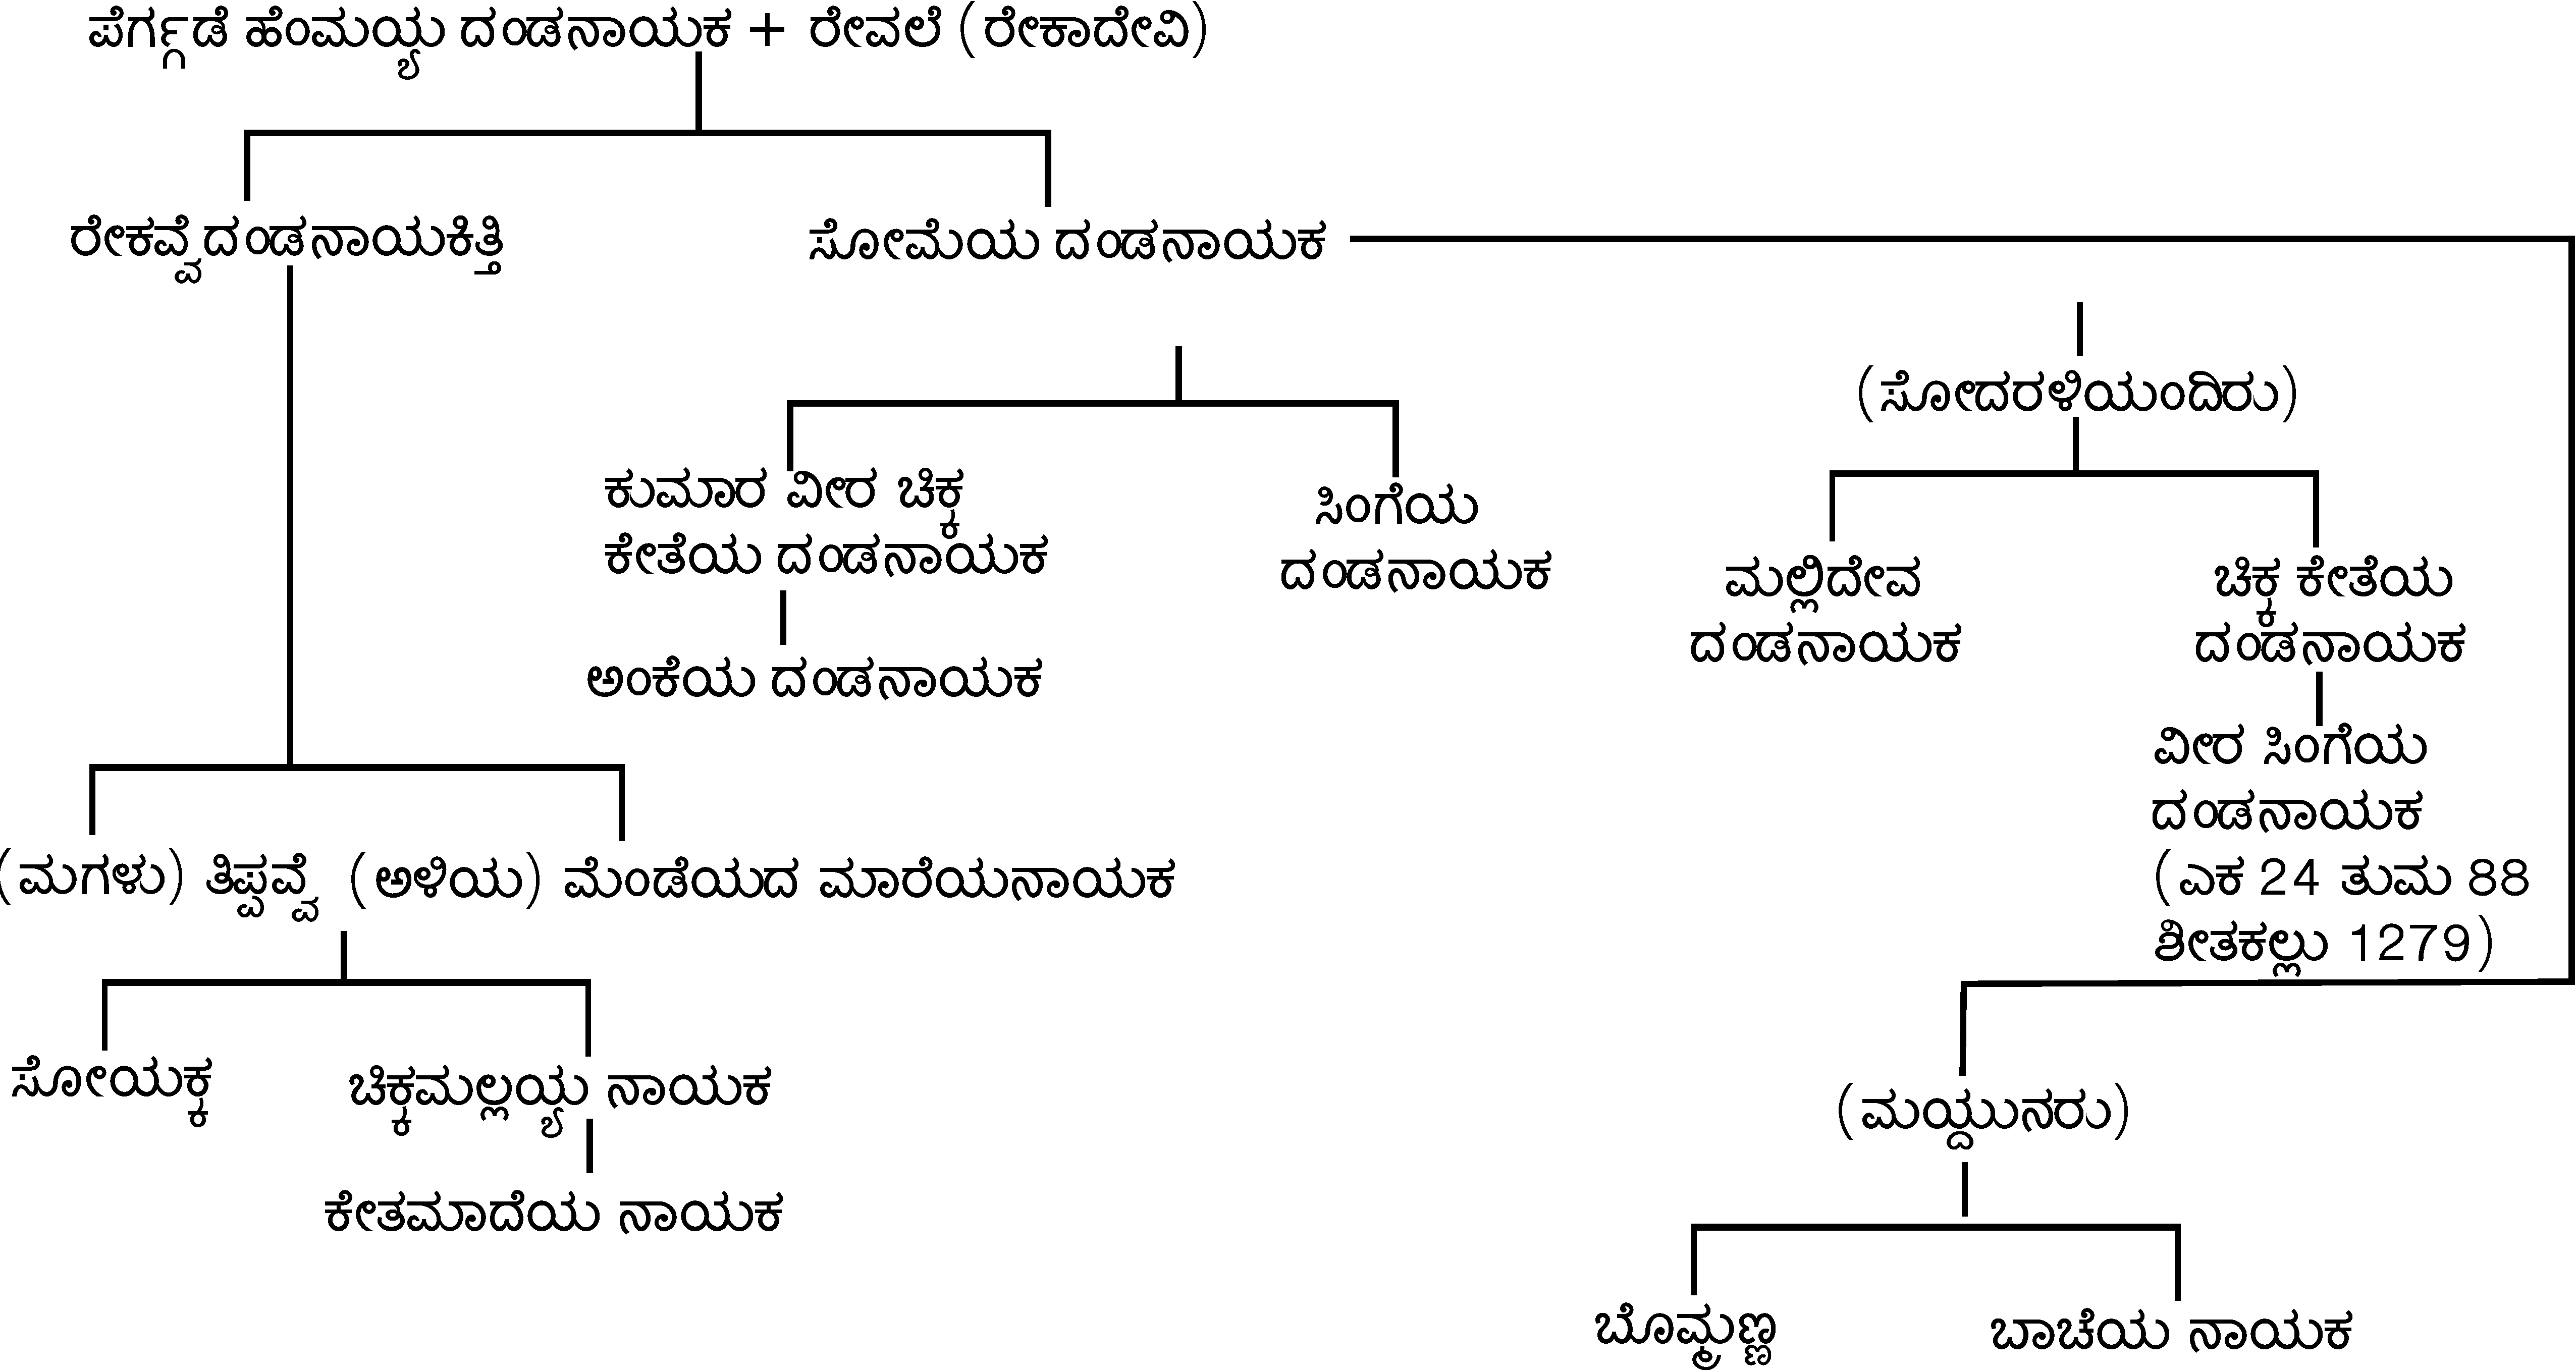
\includegraphics[scale=.8]{images/chap3/chap3fig21.jpeg}
\end{figure}

\textbf{ಮಹಾಪ್ರಧಾನ ಪ್ರಯಾಗಪೆರುಮಾಳೆ ದಂಡನಾಯಕ\index{ಮಹಾಪ್ರಧಾನ ಪ್ರಯಾಗಪೆರುಮಾಳೆ ದಂಡನಾಯಕ} (1279}): ಸರ್ವಾಧಿಕಾರಿ, ಮಹಾಪಸಾಯಿತ, ಪರಮವಿಶ್ವಾಸಿ, ಬಾಹತ್ತರ ನಿಯೋಗಾಧಿಪತಿ\index{ಬಾಹತ್ತರ ನಿಯೋಗಾಧಿಪತಿ}, ಶ‍್ರೀಕರಣ ತಿರುವಿಂದಳೂರ ಪ್ರಯಾಗಪೆರುಮಾಳೆ ದಂಡನಾಯಕನು, ಮರದುರಾದ ಶ‍್ರೀ ನಾರಸಿಂಹ ಚತುರ್ವೇದಿ ಮಂಗಲದ ವೈದ್ಯನಾಥಮುಡೆಯಾರ್​ ದೇವರಿಗೆ, ನಿಬಂಧ ಕಾಣಿಕೆಯನ್ನು, ತಿರುನಂದಾದೀಪಕ್ಕೆ ದತ್ತಿಗಳನ್ನೂ ಬಿಡುತ್ತಾನೆ.\endnote{ ಎಕ 7 ಮ 74 ವೈದ್ಯನಾಥಪುರ 1279} ಇವನು ತಮಿಳು ಪ್ರಾಂತದಿಂದ ಬಂದ ಅಧಿಕಾರಿ ಎಂದು ಎಪಿಗ್ರಾಫಿಯಾ ಸಂಪಾದಕರು ಹೇಳಿದ್ದಾರೆ.\endnote{ ಎಕ 7 ಪೀಠಿಕೆ, ಪುಟ \engfoot{lxv}} ಈತನ ಬಗ್ಗೆ ಹೆಚ್ಚಿನ ವಿವರಗಳು ತಿಳಿದುಬರುವುದಿಲ್ಲ. ಶಾಸನದ ಅರ್ಧಭಾಗ ಕಟ್ಟಡದೊಳಕ್ಕೆ ಸೇರಿಹೋಗಿದೆ. ಈತನು ಮಹಾಪ್ರಧಾನನೂ ಆಗಿದ್ದನೆಂದು ಹೇಳಬಹುದು.

\textbf{ಮಹಾಪ್ರಧಾನ ಪೆರುಮಾಳೆದೇವ ದಂಡನಾಯಕ\index{ಪೆರುಮಾಳೆ ದೇವ ದಂಡನಾಯಕ} ಮತ್ತು ಅವನ ಮಕ್ಕಳು (1271\general{\enginline{-}}1290):} ಎಡತಲೆಯ(ಹೆಡತಲೆ) ಪೆರುಮಾಳೆದೇವ ದಂಡನಾಯಕನು, ವೀರಸೋಮೇಶ್ವರ, ಮೂರನೆಯ ನರಸಿಂಹ ಮತ್ತು ಮುಮ್ಮಡಿ ವೀರಬಲ್ಲಾಳ ಇವರುಗಳ ಕಾಲದಲ್ಲಿ ಸೇನಾಧಿಪತಿಯೂ, ಮಹಾಪ್ರಧಾನ ದಂಡನಾಯಕನು, ಸಚಿವನೂ ಆಗಿದ್ದನು. ಅವನ ಮಕ್ಕಳೂ ಕೂಡಾ ಮುಮ್ಮಡಿ ಬಲ್ಲಾಳನ ಕಾಲದಲ್ಲಿ ಮಂತ್ರಿಗಳೂ ದಂಡನಾಯಕರೂ ಆಗಿದ್ದರು. “ಪೆರುಮಾಳೆ ದಂಡನಾಯಕನು ಮುಮ್ಮಡಿ ಬಲ್ಲಾಳನ ಆಳ್ವಿಕೆಯಲ್ಲೂ ಜೀವಿಸಿದ್ದನು. ಅವನಿಗೂ ಅವನ ಮಕ್ಕಳಿಗೂ ನವದಣ್ಣಾಯಕರೆಂಬ\index{ನವದಣ್ಣಾಯಕರು} ಪ್ರತೀತಿ ಇದ್ದಿತು” ಎಂದು ವಿದ್ವಾಂಸರು ಹೇಳಿದ್ದಾರೆ.\endnote{ ಕೃಷ್ಣರಾವ್​, ಡಾ॥ ಎಂ.ವಿ., ಕರ್ನಾಟಕ ಇತಿಹಾಸ ದರ್ಶನ, ಪಟ 278} ಪೆರುಮಾಳೆದೇವನು ಮೂರನೆಯ ನರಸಿಂಹನ ಮನೋಮಿತ್ರನಾಗಿದ್ದನೆಂದು ಬೇಲೂರು ಶಾಸನದಿಂದ ತಿಳಿದುಬರುತ್ತದೆ.\endnote{ ಎಕ 9 ಬೇಲೂರು 170 ಬೇಲೂರು} ಪೆರುಮಾಳೆದೇವನ ಉಲ್ಲೇಖ ಇರುವ ಮೊದಲ ಶಾಸನವೆಂದರೆ ಕ್ರಿ.ಶ.1216ರ ದೊಡ್ಡಗದ್ದವಳ್ಳಿಯ ಶಾಸನ.\endnote{ ಎಕ 8 ಹಾಸನ 38 ದೊಡ್ಡಗದ್ದವಳ್ಳಿ 1216} ಪೆರುಮಾಳೆ ದೇವನು ಶಕ ವರ್ಷ 1274 ರಲ್ಲಿ ಅಂದರೆ ಕ್ರಿ.ಶ.1351 ರಲ್ಲಿ ಮರಣ ಹೊಂದಿದನೆಂದು ಹುಲ್ಲಹಳ್ಳಿ ಶಾಸನದಿಂದ ತಿಳಿದುಬರುತ್ತದೆ.\endnote{ ಎಕ 3 ನಂಜನಗೂಡು 137 ಹುಲ್ಲಹಳ್ಳಿ 1351} ಈ ತೇದಿಗಳನ್ನು ಹಿಡಿದರೆ ಪೆರುಮಾಳೆಯ ಆಯಸ್ಸು 150 ವರ್ಷವಾಗಿಬಿಡುತ್ತದೆ. ದೊಡ್ಡಗದ್ದವಳ್ಳಿ ಶಾಸನೋಕ್ತ ಪೆರಮಾಳೆಯು ಬೇರೆ ವ್ಯಕ್ತಿಯಾಗಿರಬಹುದು.

ಪೆರಮಾಳೆದೇವನ ಬಗ್ಗೆ ಇನ್ನೊಂದು ಪ್ರಾಚೀನ ದಾಖಲೆ ಎಂದರೆ 13ನೇ ಶತಮಾನದ ಲಿಪಿಯಲ್ಲಿರುವ (ಸುಮಾರು 1230\enginline{-}40) ಮರಸೆಯ ಶಾಸನ. \textbf{ಈ ಶಾಸನದ ಪ್ರಕಾರ ಪೆರುಮಾಳೆದೇವನು ಇನ್ನೂ ಸೇನಾಧಿಪತಿಯಾಗಿದ್ದನು}.\endnote{ ಎಕ 5 ಮೈಸೂರು 191 ಮರಸೆ ಸು.13ನೇ ಶತಮಾನ.} ಸೋಮೇಶ್ವರನ ಕ್ರಿ.ಶ.1247ರ ಎಡೂರು ಶಾಸನವು ಪೆರುಮಾಳೆ ದೇವನು ಮಹಾಪ್ರಧಾನ ದಂಡನಾಯಕನಾಗಿದ್ದನೆಂದು ತಿಳಿಸುತ್ತದೆ.\endnote{ ಎಕ 4 ಚಾಮರಾಜನಗರ 128 ಎಡೂರು 1247} ಇದನ್ನು ಅನುಲಕ್ಷಿಸಿ ಎಪಿಗ್ರಾಫಿಯಾ ಸಂಪಾದಕರು “ಸೋಮೇಶ್ವರನ ಮಗ ಮುಮ್ಮಡಿ ನರಸಿಂಹನ\index{ಮುಮ್ಮಡಿ ನರಸಿಂಹ} ಆಡಳಿತಾವಧಿಯಲ್ಲಿ ಆ ಹೆಸರಿನ ಪ್ರಖ್ಯಾತ ಸೇನಾಪತಿ ಇದ್ದು ಆತನೇ ಮುಮ್ಮಡಿ ಬಲ್ಲಾಳನ ಕಾಲದಲ್ಲೂ ಅಧಿಕಾರವನ್ನು ಮುಂದುವರೆಸಿದನೆಂಬುದು ಗೊತ್ತಿರುವ ವಿಷಯ. ಪ್ರಕೃತ ಶಾಸನದಲ್ಲಿ ಉಕ್ತನಾಗಿರುವ ಸೇನಾಪತಿಯು ಆತನೇ ಎಂದು ಗುರುತಿಸಿದೆ. ಈ ಪೆರುಮಾಳೆದೇವನು ಸೋಮೇಶ್ವರನ ಕಾಲದಲ್ಲಿ ಬಹಳ ಚಿಕ್ಕವನಾಗಿರುವಾಗಲೇ ಅಧಿಕಾರ ವಹಿಸಿಕೊಂಡಿರಬಹುದೆಂದು ಊಹಿಸಿ 50 ವರ್ಷಕ್ಕೂ ಹೆಚ್ಚು ಕಾಲ ಅಧಿಕಾರದಲ್ಲಿದ್ದು ಮುಮ್ಮಡಿ ಬಲ್ಲಾಳನ ಆಳ್ವಿಕೆಯ ಪೂರ್ವಾರ್ಧದವರೆಗೆ ಜೀವಿಸಿದ್ದನೆಂದು ಹೇಳಬಹುದು” ಎಂದು ಹೇಳಿರುವುದು ಸೂಕ್ತವಾಗಿದೆ.\endnote{ ಎಕ 4 ಪೀಠಿಕೆ, ಪುಟ \engfoot{lxxix-lxxx}} ಈತನು ಆತ್ರೇಯ ಗೋತ್ರದವನು ಮೋಡಕುಲದವನು\index{ಮೋಡಕುಲ}, ರಾಮಕೃಷ್ಣ\index{ರಾಮಕೃಷ್ಣ ಗುರು} ಇವನ ಗುರು.\endnote{ ಎಕ 7 ನಾಮಂ 74 ಬೆಳ್ಳೂರು 1271} ಇವನ ತಂದೆ ವಿಷ್ಣುಚಮೂಪತಿ\index{ವಿಷ್ಣು ದಂಡಾಧೀಶ}, ತಾಯಿ ಮಂಚಲಾದೇವಿ\index{ಮಂಚಲಾದೇವಿ}.\endnote{ ಎಕ 9 ಬೇಲೂರು 170 ಬೇಲೂರು., ಎಕ 7 ನಾಮಂ 73 ಬೆಳ್ಳೂರು 1309} ವಿಷ್ಣುದೇವನಿಗೆ ಭೀಮದೇವ\index{ಭೀಮದೇವ} ಎಂಬ ಹೆಸರೂ ಇದ್ದಿತು.\endnote{ ಎಕ 3 ನಂಜನಗೂಡು 329 ಹೆಮ್ಮರಗಾಲ 1292, ಎಕ 4 ಚಾನ 309 ಕೊತ್ತಲವಾಡಿ} ಪೆರುಮಾಳೆ ದೇವನ ಹೆಂಡತಿಯ ಹೆಸರು ಅಲ್ಲಾಂಬಾ.\endnote{ ಎಕ 3 ನಂಗೂ 137 ಹುಲ್ಲಹಳ್ಳಿ 1351} ತಂಗಿ ಬಸವಿಯಕ್ಕ\index{ಬಸವಿಯಕ್ಕ}.\endnote{ ಎಕ 7 ನಾಮಂ 74 ಬೆಳ್ಳೂರು 1271} ಪೆರುಮಾಳೆ ದೇವನಿಗೆ ಲಕ್ಷ್ಮೀನಾರಾಯಣದಂಡನಾಯಕ\index{ಲಕ್ಷ್ಮೀನಾರಾಯಣದಂಡನಾಯಕ},\endnote{ ಎಕ 4 ಚಾನ 108 ಆಲದೂರು 1285} ಚಕ್ರವರ್ತಿ ದಂಡನಾಯಕ\index{ಚಕ್ರವರ್ತಿ ದಂಡನಾಯಕ},\endnote{ ಎಕ 7 ನಾಮಂ 76 ಬೆಳ್ಳೂರು 1309} ಮಾಧವ ದಂಡನಾಯಕ\index{ಮಾಧವ ದಂಡನಾಯಕ}, ಕೇತೆಯ ದಂಡನಾಯಕ\index{ಕೇತೆಯ (ಕೇತಣ್ಣ-ಕೇತಯ್ಯ-ಕೇತಪ್ಪ) ದಂಡನಾಯಕ (ದಂಣ್ನಾಯಕ)},\endnote{ ಎಕ 4 ಚಾನ 309 ಕೊತ್ತಲವಾಡಿ 1303

ಎಕ 6 ಪಾಂಪು 161 ಮೇಲುಕೋಟೆ ಸು. 1320

ಎಕ 6 ಪಾಂಪು 220 ಕದಲಗೆರೆ} ಅಲ್ಲಪ್ಪ ದಂಡನಾಯಕ\index{ಅಲ್ಲಪ್ಪ ದಂಡನಾಯಕ},\endnote{ ಎಕ 4 ಚಾನ 306 ಕಿಲಗೆರೆ 14ನೇ ಶ.} ಹೆಗ್ಗಡೆದೇವ\index{ಹೆಗ್ಗಡೆದೇವ},\endnote{ ಎಕ 3 ಹೆಕೋ 47 ಬಪ್ಪನಹಳ್ಳಿ 1327} ಮಂಚಯದಂಡನಾಯಕ\index{ಮಂಚಯದಂಡನಾಯಕ},\endnote{ ಎಕ 9 ಬೇಲೂರು 565 ನರಸೀಪುರ 1318} ಪೊನ್ನಪ್ಪ\index{ಪೊನ್ನಪ್ಪ},\endnote{ \engfoot{EC IX DB 57 Kakolu 1271}} ಮತ್ತು ಸಿಂಗೆಯ ದಂಡನಾಯಕ\index{ಸಿಂಗೆಯ ದಂಡನಾಯಕ (ದಂಣ್ನಾಯಕ)},\endnote{ ಎಕ 4 ಪಿರಿಯಾಪಟ್ಟಣ 19 ಹಳಗನಹಳ್ಳಿ 1338} ಎಂಬ ಒಂಬತ್ತು ಜನ ಮಕ್ಕಳಿದ್ದುದು ಶಾಸನಧಾರಗಳಿಂದ ತಿಳಿದುಬರುತ್ತದೆ. ಇವರೇ ನವ ದಂಡನಾಯಕರುಗಳೆಂದು ಹೆಸರು ಗಳಿಸಿರಬಹುದು.

ಇವರಲ್ಲಿ ಮಾಧವ ದಂಡನಾಯಕ ಮತ್ತು ಕೇತೆಯ ಅಥವಾ ಕಿತ್ತಪ್ಪ ದಂಡನಾಯಕರು ಮಹಾಪ್ರಧಾನ ದಂಡನಾಯಕರು\-ಗಳಾಗಿ ಮೂರನೇ ಬಲ್ಲಾಳನ ಕಾಲದವರೆಗೆ ಆಳ್ವಿಕೆ ನಡೆಸಿದರು. ಪೆರುಮಾಳೆ ದೇವನಿಗೆ ಇಬ್ಬರು ಹೆಣ್ಣುಮಕ್ಕಳಿದ್ದರು ಆದರೆ ಅವರ ಹೆಸರು ತಿಳಿದುಬರುವುದಿಲ್ಲ. ಆದರೆ ಅವನ ಇಬ್ಬರು ಅಳಿಯಂದಿರಾದ ರುದ್ರಣ್ಣ ಮತ್ತು ವರದಯ್ಯ ಇವರ ವಿಚಾರ ಬೇಲೂರು ಶಾಸನದಿಂದ ತಿಳಿದುಬರುತ್ತದೆ.\endnote{ ಎಕ 9 ಬೇಲೂರು 53 ಬೇಲೂರು 1297} ಪೆರುಮಾಳೆದೇವ ದಂಡನಾಯಕನ ಮಗ ಮಾಧವ ದಂಡನಾಯಕನಿಗೆ ಭರತಜೀಯ ದಂಡನಾಯಕ ಮತ್ತು ವೀರಕೇತೆಯ ದಂಡನಾಯಕ ಎಂಬ ಇಬ್ಬರು ಮಕ್ಕಳಿದ್ದರು.\endnote{ ಎಕ 3 ಗುಂಡ್ಲುಪೇಟೆ 40 ರಾಘವಾಪುರ 1320} “ಮಾಧವನಿಗೆ ಕೇತಯ್ಯ ಮತ್ತು ಸಿಂಗಯ್ಯ ಎಂಬ ಇಬ್ಬರು ಮಕ್ಕಳಿದ್ದರು” ಎಂದು ಕೃಷ್ಣರಾವ್​ ಹೇಳಿದ್ದಾರೆ.\endnote{ ಕೃಷ್ಣರಾವ್​, ಡಾ॥ ಎಂ.ವಿ., ಕರ್ನಾಟಕ ಇತಿಹಾಸ ದರ್ಶನ, ಪುಟ 278} ಇವರು ಪದಿನಾಲ್ಕು ನಾಡನ್ನು ತೆರಕಣಾಂಬಿಯಿಂದ ಆಳುತ್ತಿದ್ದರು. ಪೆರುಮಾಳೆ ದೇವದಂಡನಾಯಕನಿಗೆ ಶ‍್ರೀಮನ್​ ಮಹಾಪ್ರಧಾನ ಗೋಪಿಯ ದಂಡನಾಯಕ, ಅಲ್ಲಾಳದೇವ ದಂಡನಾಯಕ, ಎಂಬ ಅಣ್ಣಂದಿರೂ, ಭೀಮೆಯ ದಂಡನಾಯಕನೆಂಬ ತಮ್ಮನೂ ಇದ್ದರೆಂದು ತಿಳಿದುಬರುತ್ತದೆ.\endnote{ ಎಕ 3 ನಂಗೂ 329 ಹೆಮ್ಮರಗಾಲ 1292}

ಹೊಯ್ಸಳರಾಜ್ಯವನ್ನು ಮುತ್ತಿದ ಸೇವುಣ\index{ಸೇವುಣರು} ಸೇನೆಯನ್ನು ಹೊಡೆದೋಡಿಸುವಲ್ಲಿ ಪೆರುಮಾಳೆದೇವನು ಪ್ರಮುಖಪಾತ್ರ\-ವಹಿಸಿದ್ದನು. ಕ್ರಿ.ಶ.1271 ಕ್ಕೂ ಮುಂಚೆಯೇ ಯಾದವ ರಾಜನಾದ ಮಹದೇವನು ಹೊಯ್ಸಳ ರಾಜ್ಯದ ಮೇಲೆ ಅಪಾರಸೈನ್ಯ ಸಮೇತನಾಗಿ ನರಸಿಂಹನನ್ನೂ ಲೆಕ್ಕಿಸದೆ ದಂಡೆತ್ತಿಬಂದನು.\endnote{ ಕೃಷ್ಣರಾವ್​ ಡಾ॥ಎಂ.ವಿ., ಕರ್ನಾಟಕದ ಇತಿಹಾಸ ದರ್ಶನ, ಪುಟ 272-73} ರತ್ನಪಾಲ, ಹರಪಾಲ ಎಂಬುವವರು ಈ ಸೈನ್ಯದ ಸೇನಾಧಿಪತಿ\-ಗಳಾಗಿದ್ದರು. ಪೆರಮಾಳೆದೇವನು ಕಲಿರತ್ನಪಾಲನನ್ನು\index{ಕಲಿರತ್ನಪಾಲ} ಕೊಂದು ಜವನಿಕೆ ನಾರಾಯಣ\index{ಜವನಿಕೆ ನಾರಾಯಣ} ಎಂಬ ಬಿರುದನ್ನು ಪಡೆದನು. ತನ್ನ ಸೇನೆಯ ಸೋಲನ್ನು ನೋಡಿದ ಮಹಾದೇವನು\index{ಮಹಾದೇವ} ಮಹದೇವರಾಣೆ ತನ್ನ ತುರಗಗಳನ್ನೆಲ್ಲಾ ಬಿಟ್ಟು ಓಡಿಹೋದನು. ಈ ರೀತಿ ಸೇವುಣರ ತುರಗಗಳನ್ನು ವಶಪಡಿಸಿಕೊಂಡಿದ್ದರಿಂದ ಪೆರಮಾಳೆ ದೇವನಿಗೆ ರಾವುತ್ತರಾಯ\index{ರಾವುತ್ತರಾಯ} ಎಂಬ ಬಿರುದು ಬಂದಿರಬಹುದು. ಈ ಘಟನೆಯನ್ನು ಹೇಳುವ ಪದ್ಯಗಳನ್ನು ಪೆರುಮಾಳೆದೇವನ ಬೆಳ್ಳೂರು\index{ಬೆಳ್ಳೂರು} ಹಾಗೂ ಇತರ ಎಲ್ಲ ಪ್ರಮುಖ ಶಾಸನಗಳಲ್ಲಿ ನಾವು ಕಾಣಬಹುದು.

\begin{verse}
\textbf{ಜವನಿಕೆಯೊಡಲಿರ್ವ್ವಲದ ವೀರಭಟಾವಳಿ ನೋಡೆ ಖಳ್ಗದಿಂ} \\\textbf{ದವೆ ಕಲಿರತ್ನಪಾಲನ ಸಿರೋಂಬುಜಮಂ ಜಯಲಕ್ಷ್ಮಿಗಿತ್ತು} \\\textbf{ತಜ್ಜವನಿಕೆಗೊಂಡಗಂಡ ಪೆರುಮಾಳೆಚಮೂಪತಿಗಿಂತು ಸಾರ್ದ್ದುದಾ} \\\textbf{ಜವನಿಕೆ ನಾರಣಾಂಕವಿದು ರಾವುತರಾಯನುದಗ್ರದೊರ್ವ್ವಳಂ}
\end{verse}

\begin{verse}
\textbf{ಮದವದುಗ್ರವೈರಿಮದಮರ್ದ್ಧನ ವೀರನೃಸಿಂಹ ಭೂಬುಜಂ} \\\textbf{ಗದಿರದೆ ಬಂದು ಸೇವುಣ ಮಹಾಮಹಿಪಂ ಮಹದೇವರಾಣೆಯಿಂ} \\\textbf{ಕದನದೊಳಾಂತು ನಿತ್ತರಿಸಲಾರದೆ ಬಿಟ್ಟು ತುರುಗಮಂಗಳಂ} \\\textbf{ಬೆದರೆ ಪಲಾಯನಂ ಕುಶಲಮೆಂದೋಡಿದನೊಂದೆ ರಾತ್ರಿಯೊಳ್​}
\end{verse}

ಈ ವಿಜಯದ ನಂತರ ಪೆರುಮಾಳೆ ದೇವ ದಂಡನಾಯಕ ಮತ್ತು ಅವನ ಮಕ್ಕಳು ನೀಲಗಿರಿ\index{ನೀಲಗಿರಿ} ಕೊಂಗು\index{ಕೊಂಗು} ಪ್ರಾಂತಗಳನ್ನು ವಶಪಡಿಸಿಕೊಂಡು, ಮೂರನೇ ನರಸಿಂಹ ಮತ್ತು ಮೂರನೇ ಬಲ್ಲಾಳನ ಕಾಲದಲ್ಲಿ ತಮಿಳುನಾಡಿನ ದಂಡಯಾತ್ರೆಯನ್ನು ಕೈಗೊಂಡು ಪಾಂಡ್ಯರು ಮುಂತಾದವರನ್ನು ಸೋಲಿಸಿರಬಹುದು. \textbf{ಶ‍್ರೀಮನ್​ ಮಹಾಪ್ರಧಾನ ಪೆರುಮಾಳೆದೇವನಿಗೆ “ಸ್ವಾಮಿವಂಚಕರಗಂಡ, ರಾವುತ್ತರಾಯ, ಜವನಿಕೆ ನಾರಾಯಣ, ಶ‍್ರೀರಾಮಕೃಷ್ಣದೇವರ ಪಾದಪದ್ಮಾರಾಧಕ, ಇಮ್ಮಡಿ ರಾವುತ್ತರಾಯ\index{ರಾವುತ್ತರಾಯ}, ನೀಲಗಿರಿ ಸಾಧಾರ\index{ನೀಲಗಿರಿ ಸಾಧಾರ}, ಶಿತಕರಗಂಡ”} ಎಂಬ ಬಿರುದುಗಳಿದ್ದವು.\endnote{ ಎಕ 7 ನಾಮಂ 73, 74, 76 ಬೆಳ್ಳೂರು ಮತ್ತು ಎಕ 4 ಚಾನ 296 ನರಸಮಂಗಲ}

ಈ ವಿಜಯದ ಗಳಿಸಿಕೊಟ್ಟಿದ್ದಕ್ಕಾಗಿಯೇ ವೀರನರಸಿಂಹನು ಶಕವರ್ಷ 1184 ರಲ್ಲಿ ಅಂದರೆ, ಕ್ರಿ.ಶ.1261 ರಲ್ಲಿ ಕಲುಕಣಿ ನಾಡ ಬೆಳ್ಳೂರ ವೃತ್ತಿಯ, ಬೆಳ್ಳೂರು ಹಾಗೂ ಅದರ 25 ಕಾಲುವಳ್ಳಿಗಳ ಸಮೇತ (ಹೆಸರಿಸಿದೆ) ಅಗ್ರಹಾರವನ್ನಾಗಿ ಮಾಡಲೋಸುಗ ಪೆರುಮಾಳೆದೇವ ದಂಡನಾಯಕನಿಗೆ\index{ಪೆರುಮಾಳೆ ದೇವ ದಂಡನಾಯಕ} ಧಾರಾಪೂರ್ವಕವಾಗಿ ಕೊಟ್ಟಿರಬಹುದೆಂದು ತೋರುತ್ತದೆ. ಪೆರುಮಾಳೆ ದೇವನು ಬೆಳ್ಳೂರನ್ನು ಉದ್ಭವನರಸಿಂಹಪುರವೆಂಬ\index{ಉದ್ಭವ ನರಸಿಂಹಪುರ (ಬೆಳ್ಳೂರು)} ಅಗ್ರಹಾರವನ್ನಾಗಿ ಮಾಡಿ, ಅನೇಕ ದೇವಾಲಯಗಳನ್ನು ನಿರ್ಮಿಸಿ, ಕೆರೆಗಳನ್ನು ಕಟ್ಟಿಸಿ, ಅನ್ನಛತ್ರ, ಶಾಲೆಗಳನ್ನು ಏರ್ಪಡಿಸಿ, 86 ವೃತ್ತಿಗಳನ್ನಾಗಿ ವಿಂಗಡಿಸಿ ಸಮಸ್ತ ವಿದ್ಯಾ ವಿಶಾರದರಪ್ಪ ಬ್ರಾಹ್ಮಣರಿಗೆ ದತ್ತಿಯಾಗಿ ಬಿಟ್ಟನು.\endnote{ ಎಕ 9 ಬೇಲೂರು 170 ಬೇಲೂರು ತಾಮ್ರಶಾಸನ 1261}

ಬೆಳ್ಳೂರಿನಲ್ಲಿ ಪೆರುಮಾಳೆದೇವನು ಅಲ್ಲಾಳಸಮುದ್ರವೆಂಬ ಕೆರೆಯನ್ನು ಕಟ್ಟಿಸಿ ಅದನ್ನ ವಿಸ್ತರಿಸುತ್ತಾನೆ.\endnote{ ಎಕ 7 ನಾಮಂ 84 ಬೆಳ್ಳೂರು 1269} ಜೊತೆಗೆ ಅಲ್ಲಿ ಅವ್ವೆಯರಕೆರೆ ಮತ್ತು ತಗಚೆಗೆರೆಗಳನ್ನು ನಿರ್ಮಿಸುತ್ತಾನೆ.\endnote{ ಎಕ 7 ನಾಮಂ 83 ಬೆಳ್ಳೂರು 1269} ಕ್ರಿ.ಶ.1284 ರಲ್ಲಿ ಈ ಬೆಳ್ಳೂರಿಗೆ ಸಮೀಪದ ಬೆಟ್ಟದಕೋಟೆ\index{ಬೆಟ್ಟದಕೋಟೆ}, ಬಿಲ್ಲಬೆಳಗುಂದ\index{ಬಿಲ್ಲಬೆಳಗುಂದ}, ಮತ್ತು ತಿಪ್ಪೂರು\index{ತಿಪ್ಪೂರು} ಗ್ರಾಮಗಳನ್ನು ಅವುಗಳಿಗೆ ಸೇರಿದ ಕಾಲುವಳ್ಳಿಗ ಸಮೇತ ವೀರನರಸಿಂಹನಿಂದ ಪಡೆದು, ಅವುಗಳನ್ನು ಬೆಳ್ಳೂರು ವೃತ್ತಿಗೆ ಸೇರಿಸಿ, ಈ ಮೊದಲು ಮಾಡಿದ್ದ 86 ವೃತ್ತಿಗಳಿಗೆ ಇನ್ನು ಹತ್ತು ವೃತ್ತಿಗಳನ್ನು ಸೇರಿಸಿ, ಒಟ್ಟು 96 ವೃತ್ತಿಗಳನ್ನಾಗಿ ಮಾಡಿ ಆ ಸಮಸ್ತ ಹಳ್ಳಿಗಳಿಗೆ ತೆರಿಗೆಗಳನ್ನು ಪುನರ್​ನಿಗದಿಪಡಿಸಿ ಅಲ್ಲಿನ ಮಹಾಜನಗಳಿಗೆ ಪುನಃ ಹಂಚಿಕೆ ಮಾಡುತ್ತಾನೆ.\endnote{ ಎಕ 7 ನಾಮಂ 76 ಬೆಳ್ಳೂರು 1309} ಪೆರುಮಾಳೆದೇವನ ಮಗನಾದ ಚಕ್ರವರ್ತಿ ದಂಡನಾಯಕನು ಈ 96 ವೃತ್ತಿಗಳನ್ನು ಮಹಾಜನರಿಂದ ಖರೀದಿಸಿ, ಅವುಗಳ ತೆರಿಗೆಯ ಕೆಲವು ಭಾಗಗಳನ್ನು ದೇವಾಲಯಗಳಿಗೆ ಹೆಚ್ಚಾಗಿ ನೀಡಿ, ಉಳಿದ ವೃತ್ತಿಗಳನ್ನು ಮಹಾಜನರಿಗೆ ಪುನಃ ಕ್ರಿ.ಶ.1309 ರಲ್ಲಿ ಹಂಚಿಕೆ ಮಾಡುತ್ತಾನೆ.\endnote{ ಎಕ 7 ನಾಮಂ 76 ಬೆಳ್ಳೂರು 1309} ಪೆರುಮಾಳೆದೇವನು ಹಾದಿರವಾಗಿಲನ್ನು\index{ಹಾದಿರವಾಗಿಲು} (ಇಂದಿನ ಹಾಗಲಹಳ್ಳಿ) (ತಿಪ್ಪೂರು ತೀರ್ಥದ ಹಾದರವಾಗಿಲು\index{ತಿಪ್ಪೂರು ತೀರ್ಥದ ಹಾದರವಾಗಿಲು}) ಅಗ್ರಹಾರವನ್ನಾಗಿ ಮಾಡಿದ ವಿಚಾರ ಅಲ್ಲಿರುವ ತ್ರುಟಿತ ಶಾಸನದಿಂದ ತಿಳಿದುಬರುತ್ತದೆ.\endnote{ ಎಕ 7 ಮ 81 ಹಾಗಲಹಳ್ಳಿ 1292} ಪೆರುಮಾಳೆ ದೇವನು ಬೆಳ್ಳೂರಿನಲ್ಲಿ ವೇದಪಾಠಶಾಲೆಯನ್ನು ಮತ್ತು ಕನ್ನಡ ಬಾಲಶಿಕ್ಷೆಯನ್ನೂ\index{ಕನ್ನಡ ಬಾಲಶಿಕ್ಷೆ} ವ್ಯವಸ್ಥೆ ಮಾಡಿ ಅದರ ನಿರ್ವಹಣೆಗೆ ಮಹಾಜನಗಳಿಂದ ಗದ್ದೆಬೆದ್ದಲುಗಳನ್ನು ದತ್ತಿಯಾಗಿ ಬಿಡಿಸಿದನು.\endnote{ ಎಕ 7 ನಾಮಂ 74 ಬೆಳ್ಳೂರು 1271} ಬೆಳ್ಳೂರಿನಲ್ಲಿ ನಿತ್ಯ ಪ್ರವಾಸಿಗರಾದ ಬ್ರಾಹ್ಮಣರಿಗಾಗಿ ಅನ್ನಸತ್ರವನ್ನು ಏರ್ಪಡಿಸಿದನು.\endnote{ ಎಕ 7 ನಾಮಂ 83 ಬೆಳ್ಳೂರು 1269} ಉದ್ಭವಸರ್ವಜ್ಞ ಶ‍್ರೀರಂಗಪುರವಾದ\index{ಉದ್ಭವಸರ್ವಜ್ಞ ಶ‍್ರೀರಂಗಪುರ} ಮಾಯಿಲಂಗೆಯಲ್ಲಿ\index{ಮಾಯಿಲಂಗೆ (ಲಿಂಗಿ)} (ಇಂದಿನ ತಡಿಮಾಲಿಂಗಿ\index{ತಡಿಮಾಲಿಂಗಿ}) ವೇದ ಪಾಠಶಾಲೆ ಮತ್ತು ಬಾಲಶಿಕ್ಷೆ ಎಂದರೆ ಕನ್ನಡ ಪಾಠಶಾಲೆಗಳನ್ನು ಏರ್ಪಡಿಸಿದನು.\endnote{ ಎಕ 5 ತಿ ನರಸಿಪುರ 238 ತಡಿಮಾಲಿಂಗಿ 1290} ಪೆರುಮಾಳೆದೇವನು ಉದ್ಭವವಿಶ್ವನಾಥಪುರ(ಬಾಳಗಂಚಿ)\index{ಉದ್ಭವ ವಿಶ್ವನಾಥಪುರ(ಬಾಳಗಂಚಿ)},\endnote{ ಎಕ 10 ಚರಾಪ 134 ಬಾಳಗಂಚಿ 1276} ವಿಜಯಸೋಮನಾಥಪುರ (ಹೊಳೆನರಸಿಪುರ),\endnote{ ಎಕ 8 ಹೊನಪು 1 ಹೊಳೆನರಸಿಪುರ 1276} ಬಿಜ್ಜಲಾಪುರ(ಹಾನುಗಲ್ಲು),\endnote{ ಎಕ 8 ಅಗೂ 39 ಹಾನುಗಲ್ಲು 1280} ಸರ್ವಜ್ಞ ಶ‍್ರೀರಂಗಪುರವಾದ ಮಾಯಿಲಂಗೆ,\endnote{ ಎಕ 5 ತಿ ನರಸಿಪುರ 238 ತಡಿಮಾಲಿಂಗಿ 1290} ಇವುಗಳನ್ನು ಅಗ್ರಹಾರವನ್ನಾಗಿ ಮಾಡಿ ಅಲ್ಲಿನ ಶೈವ ಮತ್ತು ವೈಷ್ಣವ ದೇವಾಲಯಗಳಿಗೆ ದತ್ತಿ ನೀಡಿದನು.

ಪೆರುಮಾಳೆ ದೇವನಿಗೆ ಚಿಮ್ಮತ್ತನಕಲ್ಲು\index{ಚಿಮ್ಮತ್ತನಕಲ್ಲು} ಅಂದರೆ ಇಂದಿನ ಚಿತ್ರದುರ್ಗವು\index{ಚಿತ್ರದುರ್ಗ} ವೃತ್ತಿಯಾಗಿ ಬಂದಿತ್ತು. ಶಕವರ್ಷ 1208 ರಲ್ಲಿ (ಕ್ರಿ.ಶ.1286) ಎಸಗೂರು ಮತ್ತು ಬೆಣ್ಣೆದೊಣೆಯಲ್ಲಿ ಸಾಕಷ್ಟು ಭೂಮಿಯನ್ನು ಖರೀದಿಸಿ ಪಾಂಡವರಿಂದ ಪ್ರತಿಷ್ಠೆಯಾದ ಅಲ್ಲಿನ ಧರ್ಮೇಶ್ವರದೇವರೇ ಮೊದಲಾದ ಪಂಚಲಿಂಗಗಳಿಗೆ ಮತ್ತು ರಂಗನಾಥ ದೇವರುಗಳಿಗೆ ದತ್ತಿ ಬಿಟ್ಟನು.\endnote{ ರಾಜಶೇಖರಪ್ಪ.ಬಿ., ದುರ್ಗದ ಶೋಧನೆ, ಪುಟ 61-74} ಕ್ರಿ.ಶ.1286 ರಲ್ಲಿ ಚಿಮ್ಮತ್ತನೂರಿನ ನಗರೇರ ಸೀಮೆಗೆ ಸೇರಿದ ಭೂಮಿಯನ್ನು ಖರೀದಿಸಿ, ಅರಕೆರೆಯ ರಾಮನಾಥದೇವರಿಗೆ ದತ್ತಿ ಬಿಟ್ಟನು.\endnote{ ಅದೇ, ಪುಟ 41-43} ಚಿತ್ರದುರ್ಗದಲ್ಲಿ ಪೆರುಮಾಳೆಪುರವೆಂಬ ಹೆಸರಿನ ಬ್ರಹ್ಮಪುರಿಯನ್ನು ಮಾಡಿ ಅದಕ್ಕೆ ಅನೇಕ ದತ್ತಿಗಳನ್ನು ಬಿಟ್ಟನು.\endnote{ ಅದೇ ಪುಟ 52-56}

ಪೆರುಮಾಳೆದೇವ ದಂಡನಾಯಕನು, ನಡೆವಲ್ಲಿಗೆಪುರದಲ್ಲಿದ್ದ\index{ನಡೆವಲ್ಲಿಗೆಪುರ} ತನ್ನ ತಾಯಿ ಮಂಚಿಯಕ್ಕನ\index{ಮಂಚಿಯಕ್ಕ}, ವೃಂದಾವನಕ್ಕೆ ಪೂಜಾ ವ್ಯವಸ್ಥೆ\-ಯನ್ನು ಮಾಡಿದನು.\endnote{ ಎಕ 9 ಬೇಲೂರು 562 ನರಸೀಪುರ 1280} ಬಹುಶಃ ಪೆರುಮಾಳೆದೇವನ ಬಾಲ್ಯವೆಲ್ಲ ಬೇಲೂರಿನಲ್ಲಿ ಕಳೆದಿರಬಹುದು. ಆಗ ಪೆರುಮಾಳೆ ದೇವನು ಅವನ ಸಮಕಾಲೀನನಾಗಿದ್ದ ಮೂರನೆಯ ನರಸಿಂಹನ ಮಿತ್ರನಾಗಿದ್ದಿರಬಹುದು. ಆದುದರಿಂದಲೇ ಬೇಲೂರು ಶಾಸನದಲ್ಲಿ ಪೆರುಮಾಳೆದೇವನು ನರಸಿಂಹನ ಮನೋಮಿತ್ರನಾಗಿದ್ದನೆಂದು\index{ಮನೋಮಿತ್ರ} ಹೇಳಿದೆ. ಇದರಿಂದ ಪೆರುಮಾಳೆ ದೇವನ ಜನನದ ವರ್ಷವನ್ನು ಮೂರನೆಯ ನರಸಿಂಹನ ಜನನದ ಕಾಲ ಅಂದರೆ ಕ್ರಿ.ಶ.1254ರ ಸುಮಾರಿಗೆ ಹಾಕಬಹುದು. ಈತನ ಮೃತಪಟ್ಟ ವರ್ಷ 1351 ಎಂಬುದು ಪೂರ್ವೋಕ್ತ ಹುಲ್ಲಹಳ್ಳಿ\index{ಹುಲ್ಲಹಳ್ಳಿ} ಶಾಸನದಲ್ಲಿದೆ. ಪೆರುಮಾಳೆದೇವನ ತಂದೆಯ ಹೆಸರು ವಿಷ್ಣುದೇವ ಅಥವಾ ಭೀಮದೇವ ಎಂದು ಖಚಿತವಾಗಿ ತಿಳಿದುಬರುತ್ತದೆ.\endnote{ ಎಕ 3 ನಂಜನಗೂಡು 329 ಹೆಮ್ಮರಗಾಲ 1292, ಎಕ 4 ಚಾಮರಾಜನಗರ 309 ಕೊತ್ತಲವಾಡಿ 1303} ಪೆರುಮಾಳೆ ದೇವನಿಗೆ ಇಬ್ಬರು ದೊಡ್ಡಪ್ಪಂದಿರು ಮತ್ತು ಒಬ್ಬ ಚಿಕ್ಕಪ್ಪ ಮತ್ತು ಅವರಿಗೆ ಒಬ್ಬೊಬ್ಬ ಮಕ್ಕಳಿದ್ದು ಅವರೂ ದಂಡನಾಯಕರಾಗಿದ್ದ ವಿಚಾರ ಹೆಮ್ಮರಗಾಲ ಶಾಸನದಿಂದ ತಿಳಿದುಬರುತ್ತದೆ.\endnote{ ಎಕ 3 ನಂಜನಗೂಡು 329 ಹೆಮ್ಮರಗಾಲ 1292}

\textbf{ಮಹಾಪ್ರಧಾನ ಮಾಧವ\index{ಮಹಾಪ್ರಧಾನ ಮಾಧವ} ಅಥವಾ ಮಾದಪ್ಪ (ಮಾದಿದೇವ)\index{ಮಾದಪ್ಪ (ಮಾದಿದೇವ)} ಮತ್ತು ಕೇತೆಯ ದಂಡನಾಯಕ\index{ಕೇತೆಯ (ಕೇತಣ್ಣ-ಕೇತಯ್ಯ-ಕೇತಪ್ಪ) ದಂಡನಾಯಕ (ದಂಣ್ನಾಯಕ)} (1300\general{\enginline{-}}1320): } ಇವರಿಬ್ಬರೂ ಪೆರುಮಾಳೆ ದೇವನ ಮಕ್ಕಳಾಗಿದ್ದು ಮುಮ್ಮಡಿ ಬಲ್ಲಾಳನಲ್ಲಿ ಮಂತ್ರಿಗಳೂ ದಂಡನಾಯಕರೂ ಆಗಿದ್ದರು. ಇವರಿಬ್ಬರೂ ಶಾಸನಗಳಲ್ಲಿ ಒಟ್ಟಾಗಿ ಕಾಣಿಸಿಕೊಳ್ಳುತ್ತಾರೆ. ಮಾಧವ ದಂಡನಾಯಕನನ್ನು ಶಾಸನಗಳು ಶ‍್ರೀಮನ್ಮಹಾಪ್ರಧಾನ ದಂಡನಾಯಕ ಎಂದು ಕರೆದಿವೆ. ಮಾಧವದಂಡನಾಯಕನಿಗೆ “\textbf{ಮೋಡಕುಳಕಮಳ ಮಾರ್ತಾಂಡ, ಸಿತಗರ ಗಂಡ, ಕದನಪ್ರಚಂಡ,\general{\break } ಇಮ್ಮಡಿರಾವುತ್ತರಾಯ, ಕೊಂಗಮಾರಿ, ಕೊಂಗರದಿಶಾಪಟ್ಟ, ನೀಲಗಿರಿಸಾಧಾರ\index{ನೀಲಗಿರಿ ಸಾಧಾರ}, ಗಿರಿದುರ್ಗಮಲ್ಲ, ಜಲದುರ್ಗ ಪುಂಡರಿಕ ಹೃದಯಶಲ್ಯ, ಹೊಯಿಸಳರಾಜ್ಯಲಕ್ಷ್ಮೀಪ್ರಾಕಾರ\index{ಹೊಯಿಸಳರಾಜ್ಯಲಕ್ಷ್ಮೀಪ್ರಾಕಾರ}, ಅಭಿನವಮದನಾವತಾರ, ಪಾಂಡ್ಯಪಾಡಿ ವಿಘಟನ, ಪಾಂಡ್ಯಬಲ ಕಮಲವನ ಕುಂಜರ, ಶರಣಾಗತವಜ್ರಪಂಜರ, ಹಿರಿಮಂಡಳಿಕಮಾನ ಮರ್ದ್ಧನ, ವೈರಿಮಂಡಳಿಕ ಸಂಗ್ರಾಮರಾಮ, ಅರಸುಗಂಡ,\general{\break } ರಾಮನಬೆಂಕೊಂಡಗಂಡ, ವಿಶಾಲಮುದ್ರಿ, ಗರ್ಬ್ಭಸರ್ಬ್ಬಸ್ವಾಪಹಾರ, ಕೀರ್ತ್ಯಂಗನವಲ್ಲಭ, ದುಷ್ಟಜನದುರ್ಲಭ, ಅಲ್ಲಾಳನಾಥ ದಿವ್ಯಶ‍್ರೀ ಪಾದಪದ್ಮಾರಾಧಕ, ಯೇಕಾದಶಿವ್ರತನಿರತ, ಏಕಾಂಗವೀರ, ವೀರಲಕ್ಷ್ಮೀಭುಜಂಗ, ಸಾಲಮಂನೆಯ ಬೇಂಟೆಕಾರ\index{ಸಾಲಮಂನೆಯ ಬೇಂಟೆಕಾರ}, ಅನವರತ ಕನಕಕರ್ಪ್ಪೂರಧಾರಾಪ್ರವಾಹ, ಗೋಬ್ರಾಹ್ಮಣಪ್ರಿಯ, ಪರನಾರೀಸೋದರ, ಸ್ವಸ್ತಿಪುರವರಾಧೀಶ್ವರ\general{\break } ಶ‍್ರೀಪೆರುಮಾಳೆದೇವ ದಂಣಾಯಕರ ಕುಮಾರ ಶ‍್ರೀ ಮಾಧವದಂಣಾಯಕರುಂ”} ಎಂಬ ಬಿರುದುಗಳಿದ್ದವು.\endnote{ ಎಕ 3 ಗುಂಪೇ 152 ತ್ರಿಯಂಬಕಪುರ 1310, ಎಕ 3 ಗುಂಪೇ 223 ಕಣ್ಣಾಗಾಲ 1315} ಇವುಗಳಲ್ಲಿ ಪೆರುಮಾಳೆದೇವನಿಗಿದ್ದ ಬಿರುದುಗಳೂ ಸೇರಿವೆ ಎಂದು ಹೇಳಬಹುದು.

ಇವರು ಮಂಡ್ಯ ಜಿಲ್ಲೆಯಲ್ಲೂ ಬಹಳ ಕಾಲ ನೆಲೆಸಿ ಮೇಲುಕೋಟೆ\index{ಮೇಲುಕೋಟೆ} ಮತ್ತು ಸುತ್ತಮುತ್ತಲ ಪ್ರಾಂತ್ಯಗಳ ಮೇಲೆ ಆಡಳಿತ ನಡೆಸುತ್ತಿದ್ದಂತೆ ತೋರುತ್ತದೆ. ಕೊನೆಗೆ ಇವರು ಹದಿನಾಲ್ಕು(ಹದಿನಾಡು)ನಾಡು ಮತ್ತು ಕುಡುಗುನಾಡುಗಳನ್ನು, ಅದರ ರಾಜಧಾನಿ ತೆರಕಣಾಂಬಿಯಿಂದ ಪಾಲಿಸುತ್ತಿದ್ದರು. ಕಲುಕಣಿ ನಾಡಿಗೆ ಸೇರಿದ್ದ ಕದ್ದಳಗೆರೆ\index{ಕದ್ದಳಗೆರೆ(ಕದಲಗೆರೆ)} ಹಾಗೂ ಅದರ ಉಪಗ್ರಾಮಗಳನ್ನು ಮುಮ್ಮಡಿ ವೀರಬಲ್ಲಾಳನು ಮಾದಪ್ಪ ದಂಡನಾಯಕನಿಗೆ\index{ಮಾದಪ್ಪ(ಣ್ಣ) ದಂಡನಾಯಕ} ನೀಡಿದ್ದನು, ಅದನ್ನು ಮಾದಪ್ಪ ದಂಡನಾಯಕನು ಕದ್ದಳಗೆರೆಯ ಲಕ್ಷ್ಮೀನಾರಾಯಣ ದೇವರು ಮತ್ತು ಮೇಲುಕೋಟೆಯ ತಿರುನಾರಾಯಣ ದೇವರಿಗೆ ಹಂಚಿಕೆ ಮಾಡಿದನು.\endnote{ ಎಕ 6 ಪಾಂಪು 220 ಕದಲಗೆರೆ 1300}\textbf{ ಈಗಲೂ ಮೇಲುಕೋಟೆಯ ಚೆಲುವನಾರಾಯಸ್ವಾಮಿ ವೈರಮುಡಿಯ\index{ವೈರಮುಡಿ ಉತ್ಸವ} ಉತ್ಸವ ಇದೇ ಕದ್ದಳಗೆರ(ಇಂದಿನ ಕದಲಗೆರೆ)ಯಿಂದ ಪ್ರಾರಂಭ\-ವಾಗುತ್ತದೆ.} ಮಾಧವ ದಂಡನಾಯಕನ ಅಧಿಕಾರಿ ಸೇನುಬೋವ ಪದುಮಣ್ಣನು ಹೊಸಹೊಳಲಿನ\index{ಹೊಸಹೊಳಲು} ಈಶಾನ್ಯ ಸೋಮನಾಥ ದೇವರ ಅಮ್ರಿತಪಡಿಗೆ ಮಹಾಜನಗಳ ಅನುಮತಿಯ ಮೇರೆಗೆ ಗದ್ದೆಯನ್ನು ದತ್ತಿಯಾಗಿ ಬಿಟ್ಟನು.\endnote{ ಎಕ 6 ಕೃಪೇ 8 ಹೊಸಹೊಳಲು 1306} ಮಾದಪ್ಪ ದಂಡನಾಯಕನು ವಿದ್ಯಾನಿಧಿ ಪ್ರಸನ್ನಕೇಶವಪುರ (ಬಸವಾಪುರ)\index{ವಿದ್ಯಾನಿಧಿ ಪ್ರಸನ್ನಕೇಶವಪುರ (ಬಸವಾಪುರ)}.\endnote{ ಎಕ 4 ಚಾನ 235 ಬಸವಾಪುರ 1316} ಸಕಲವಿದ್ಯಾನಿಧಿ ಪ್ರಸನ್ನಮಾಧವಪುರ(ಸತ್ಯಾಗಾಲ)\index{ಸಕಲವಿದ್ಯಾನಿಧಿ ಪ್ರಸನ್ನಮಾಧವಪುರ(ಸತ್ಯಾಗಾಲ)}.\endnote{ ಎಕ 4 ಕೊಳ್ಳೆಗಾಲ 30 ಸತ್ಯಾಗಾಲ 1321} ಇವುಗಳನ್ನು\break ಅಗ್ರಹಾರಗಳನ್ನಾಗಿ ಮಾಡಿದನು. ಮಾಧವ ದಂಡನಾಯಕನು ಮೇಲುಕೋಟೆಯಲ್ಲಿ 52 ಜನ ಶ್ರಿವೈಷ್ಣವರಿಗೆ ನೀಡಿದ್ದ ದತ್ತಿಯನ್ನು ನವೀಕರಿಸಿದನು.\endnote{ ಎಕ 6 ಪಾಂಪು 212 ಮೇಲುಕೋಟೆ 14ನೇ ಶ.}\textbf{ಎಂಬೆರುಮಾನರು\index{ಎಂಬೆರುಮಾನರು} ಅಂದರೆ ರಾಮಾನುಜಾಚಾರ್ಯರು\index{ರಾಮಾನುಜಾಚಾರ್ಯರು} ಕಂಡ ತಿರಿಮಣ್ಣ ಸಾಮ್ಯವನು\index{ತಿರಿಮಣ್ಣ ಸಾಮ್ಯ} ಅಂದರೆ ನಾಮದ ಮಣ್ಣು ಸಿಗುತ್ತಿದ್ದ ಭೂಮಿಯನ್ನು, ತಿರಿಮಣ್ಣ ಪೆರುಮಾಳಿಗೆ\index{ತಿರಿಮಣ್ಣ ಪೆರುಮಾಳಿ}, ಅಂದರೆ ಚೆಲುವನಾರಾಯಣ ಸ್ವಾಮಿಗೆ ದತ್ತಿಯಾಗಿ ಬಿಟ್ಟನು.}\endnote{ ಎಕ 6 ಪಾಂಪು 185 ಮೇಲುಕೋಟೆ 1319} ಮಾದಪ್ಪ ಮತ್ತು ಕೇತಪ್ಪ ದಂಡನಾಯಕರು ಒಟ್ಟಾಗಿ ಮೇಲುಕೋಟೆಯ ತಿರುನಾರಾಯಣ ಪೆರುಮಾಳಿಗೆ ಎಲೆಯ ಕರಿಎಮ್ಮಾಉರ ಅಂದರೆ ಇಂದಿನ ಎಲೆಚಾಕನಹಳ್ಳಿಯ\index{ಎಲೆಚಾಕನಹಳ್ಳಿ} ಕುಲವನಹಳ್ಳದಲ್ಲಿ ಗದ್ದೆಯನ್ನು, ಹದಿನೈದು ಕುಳ ತೋಟವನ್ನು ಲಕ್ಷ್ಮಣದಾಸ ಎಂಬ ವೈಷ್ಣವ ಯತಿಗೆ ದತ್ತಿಯಾಗಿ ಬಿಟ್ಟರು.\endnote{ ಎಕ 6 ಪಾಂಪು 161 ಮೇಲುಕೋಟೆ ಸು. 1320} ಮಾಧವ ಮತ್ತು ಕೇತೆಯ ದಂಡನಾಯಕರು ಪದಿನಾಲ್ಕುನಾಡಿನ ರಾಜಧಾನಿ ತೆರಕಣಾಂಬಿಯಲ್ಲಿ ಶ‍್ರೀ ವರದರಾಜ ಅಲ್ಲಾಳನಾಥ ದೇವರನ್ನು ಪ್ರತಿಷ್ಠಾಪಿಸಿ ಅದಕ್ಕೆ ಕೊತ್ತಲವಾಡಿ ಗ್ರಾಮವನ್ನು ದತ್ತಿಯಾಗಿ ಬಿಟ್ಟರು.\endnote{ ಎಕ 4 ಚಾನ 309 ಕೊತ್ತಲವಾಡಿ 1303} ಮಾಧವ ದಂಡನಾಯಕನು ಗೋವರ್ಧನಗಿರಿಯಲ್ಲಿ\index{ಗೋವರ್ಧನಗಿರಿ} ಅಂದರೆ ಇಂದಿನ ಹಿಮವದ್​ ಗೋಪಾಲಸ್ವಾಮಿ ಬೆಟ್ಟದಲ್ಲಿ\index{ಹಿಮವದ್​ ಗೋಪಾಲಸ್ವಾಮಿ ಬೆಟ್ಟ} ಗೋಪಿನಾಥದೇವರನ್ನು ಪ್ರತಿಷ್ಠಾಪಿಸಿ, ಅದಕ್ಕೆ ಮುಮ್ಮಡಿಬಲ್ಲಾಳನು ತನಗೆ ಕಾರುಣ್ಯದಿಂದ ನೀಡಿದ್ದ\break ಕುಡುಗುನಾಡೊಳಗಣ, ಕಣ್ಣವಂಗಲವನು ದತ್ತಿಯಾಗಿ ಬಿಟ್ಟನು.\endnote{ ಎಕ 3 ಗುಂಪೇ 223 ಕಣ್ಣಾಗಾಲ 1315} ಮಹಾಪ್ರಧಾನ ಮಾಧವ ದಂಡನಾಯಕನು 1015 ಗದ್ಯಾಣಗಳನ್ನು ಮೇಲುಕೋಟೆಯ ನಾರಾಯಣದೇವರ ಸೇವೆಗೆ ದತ್ತಿಯಾಗಿ ಬಿಟ್ಟನು.\endnote{ ಎಕ 6 ಪಾಂಪು 154 ಮೇಲುಕೋಟೆ 1312} ಮುಮ್ಮಡಿ ವೀರಬಲ್ಲಾಳನು\index{ಮುಮ್ಮಡಿ ಬಲ್ಲಾಳ (ವೀರ ಬಲ್ಲಾಳ)} ಆ ಸ್ಥಳದ ತೆರಿಗೆಗಳನ್ನು, ಮಾದಪ್ಪ ದಂಡನಾಯಕನು ತನ್ನ ತಮ್ಮ ಕಿತ್ತಪ್ಪ ದಂಡನಾಯಕನ\index{ಕಿತ್ತಪ್ಪ ದಂಡನಾಯಕ} ಹೆಸರಿನಲ್ಲಿ ನಡೆಸುವ ಧರ್ಮಕ್ಕೆ ದತ್ತಿ ನೀಡಿದನೆಂದು ಈ ಶಾಸನದಲ್ಲಿದೆ. ಬಹುಶಃ ಈ ವೇಳೆಗೆ ಕಿತ್ತಪ್ಪದಂಡನಾಯಕನು ಮೃತಪಟ್ಟಿರಬಹುದು. ಅದರಿಂದಾಗಿಯೇ ಅವನ ಹೆಸರಿನಲ್ಲಿ ಮಾದಪ್ಪ ದಂಡನಾಯಕನು ಪೂಜೆಯನ್ನು ಏರ್ಪಡಿಸಿ ಅದಕ್ಕೆ ರಾಜನಿಂದ ದತ್ತಿಯನ್ನು ಪಡೆದಿದ್ದಾನೆ.

\begin{figure}[H]
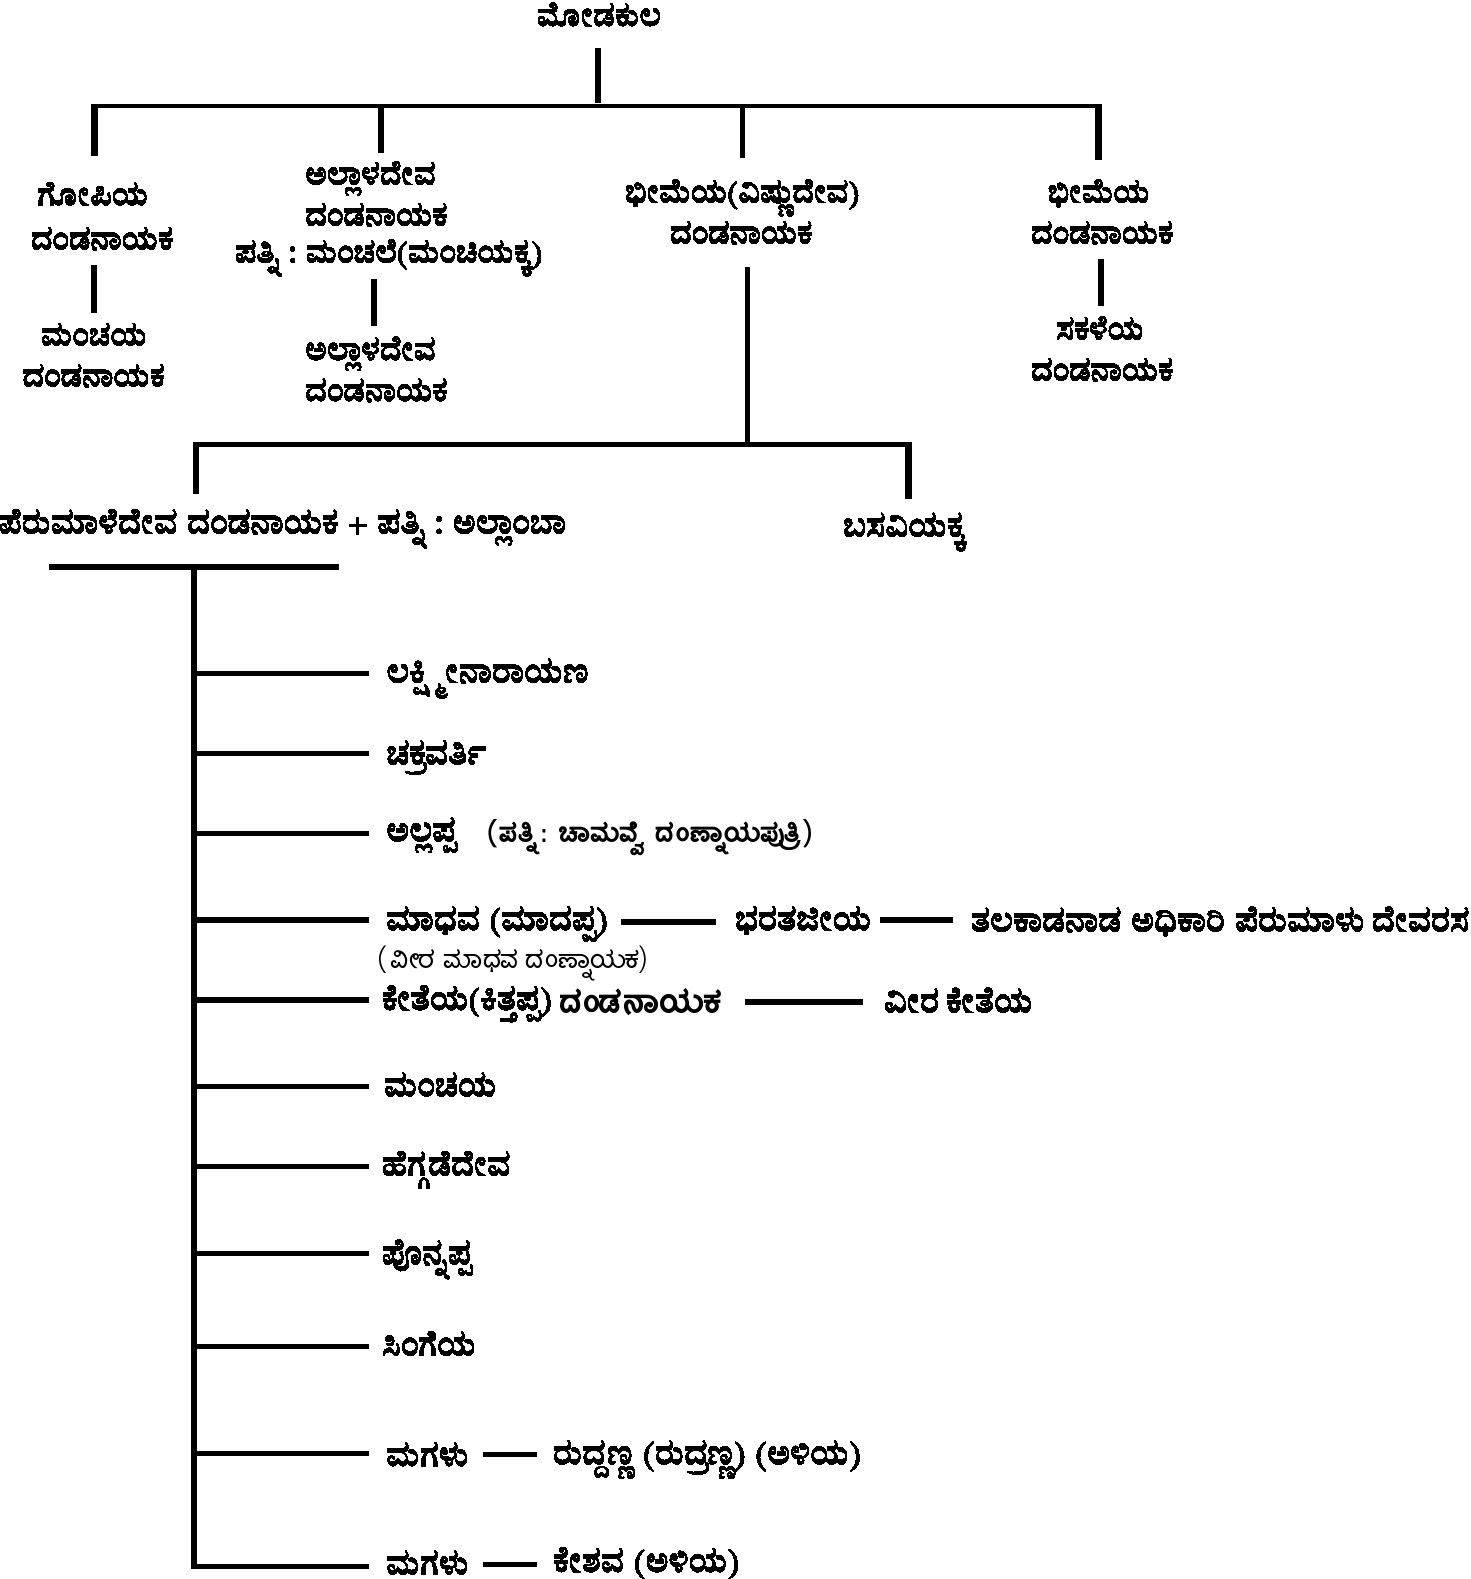
\includegraphics[scale=.28]{images/chap3/chap3fig24.jpeg}
\end{figure}

\textbf{ಪೆರುಮಾಳೆದೇವ ದಂಡನಾಯಕನು\index{ಪೆರುಮಾಳೆ ದೇವ ದಂಡನಾಯಕ} ಇತಿಹಾಸ ವಿದ್ವಾಂಸರ ಹೊಗಳಿಕೆಗೆ ಪಾತ್ರನಾಗಿದ್ದಾನೆ.\endnote{ ಕೃಷ್ಣರಾವ್​ ಡಾ॥ ಎಂ.ವಿ., ಕರ್ನಾಟಕದ ಇತಿಹಾಸ ದರ್ಶನ, ಪುಟ 274} “ಹೊಯ್ಸಳ ರಾಜ್ಯದ ಅತ್ಯಂತ ಹೆಸರಾಂತ ಸೇನಾನಿಗಳಲ್ಲಿ ಪೆರುಮಾಳೆಯೂ ಒಬ್ಬನಾಗಿದ್ದನು. ಸೋಮೇಶ್ವರ, ಮುಮ್ಮಡಿನರಸಿಂಹ ಹಾಗೂ ಮುಮ್ಮಡಿ ಬಲ್ಲಾಳ\general{\enginline{-}}ಈ ಮೂವರು ಹೊಯ್ಸಳ ದೊರೆಗಳ ಕೈಕೆಳಗೆ ಆತ ಸೇವೆ ಸಲ್ಲಿಸಿದನು. ಹೊಯ್ಸಳ ಪೋಷಕರಲ್ಲಿ ಆತ ಅತ್ಯಂತ ಶ್ರೇಷ್ಠನಾಗಿದ್ದನು. “ಲೋಕೋಪಕಾರದಲ್ಲಿ ಆತನಿಗೆ ಸರಿಗಟ್ಟುವ ಇತರ ಯಾವುದೇ ವ್ಯಕ್ತಿ ದೇಶದಲ್ಲಿ ಇದ್ದನೆನ್ನುವುದರ ಬಗ್ಗೆ ನಮಗೆ ಖಚಿತವಿಲ್ಲ. ವೈವಿಧ್ಯಮಯ ಸಂಘಸಂಸ್ಥೆಗಳಿಗೆ ಉದಾರ ಕಾಣಿಕೆಗಳನ್ನು ನೀಡುವುದರ ಮೂಲಕ ಆತನು ಗಂಗರಾಜನನ್ನೂ ಮೀರಿಸಿದನು. ಇತಿಹಾಸದಲ್ಲಿ ತಿಳಿದುಬರುವ ಯಾವುದೇ ವ್ಯಕ್ತಿಗಿಂತಲೂ ಹೆಚ್ಚಿನ ಸಂಖ್ಯೆಯಲ್ಲಿ ದೇವಾಲಯಗಳನ್ನು ಕಟ್ಟಿಸಿದನು, ಹೆಚ್ಚು ದಾನಧರ್ಮಗಳನ್ನು ಮಾಡಿದನು. ಹೆಚ್ಚು ಧಾರ್ಮಿಕ ಮಠಮಾನ್ಯಗಳನ್ನು, ಛತ್ರಗಳನ್ನು, ವಿದ್ಯಾಕೆಂದ್ರಗಳನ್ನು ಸ್ಥಾಪಿಸಿದನು ಮತ್ತು ಕೆರೆಗಳನ್ನು ಕಟ್ಟಿಸಿದನು. ಇದಕ್ಕೆ ಯಾವುದೇ ಭಾಷಿಕ, ಭೌಗೋಳಿಕ ಅಥವಾ ಮತೀಯ ಅಡೆತಡೆಗಳೂ ಆತನಿಗಿರಲಿಲ್ಲ. ಹದಿನೈದು ವೈಷ್ಣವಕೇಂದ್ರಗಳು ಮತ್ತು ಸುಮಾರು ಹನ್ನೆರಡು ಶೈವಸಂಸ್ಥೆಗಳಿಗೆ ದಾನಧರ್ಮಗಳನ್ನು ಮಾಡಿದುದರ ಜೊತೆಗೆ ಆತ ಹೊಯ್ಸಳ ಸಮಾಜದ ಶ‍್ರೀಮಂತಿಕೆಗಾಗಿ ಆರೆಂಟು ಕೆರೆಕಟ್ಟೆಗಳನ್ನು ಕಟ್ಟಿಸಿ ದಾನ ನೀಡಿದನು. ಇಷ್ಟಲ್ಲದೆ ಶ್ರೇಷ್ಠನಾದ ಮಾಧವ ದಂಡನಾಯಕನೂ ಸೇರಿದಂತೆ ಆರು ಮಂದಿ ಪುತ್ರರತ್ನರನ್ನೂ ಸಮಾಜಕ್ಕೆ ನೀಡಿದನು. ಪೆರುಮಾಳೆಯು ತಮಿಳು ಮೂಲದವನೆನ್ನುವುದು ಸ್ಪಷ್ಟ. ಆದರೆ ಶೀಘ್ರವೇ ಕನ್ನಡವನ್ನು ಕಲಿತು ತನ್ನ ಜೀವಿತಾವಧಿಯ ಬಹುಭಾಗದಲ್ಲಿ ಅಭಿವ್ಯಕ್ತಿಗೆ ಆ ಭಾಷೆಯನ್ನೇ ಮಾಧ್ಯಮವನ್ನಾಗಿ ಆರಿಸಿಕೊಂಡನು”.}\endnote{ ಪ್ರೊ॥ ಶೆಟ್ಟರ್​, ಉದೃತ ಎಪಿಗ್ರಾಫಿಯಾ ಕರ್ನಾಟಿಕಾ, ಸಂಪುಟ 10, ಪೀಠಿಕೆ ಪುಟ \engfoot{lix-lx}}

\vskip 2pt

ಪೆರುಮಾಳೆದೇವನ ವಂಶವೃಕ್ಷವನ್ನು, ರಾಧಾ ಪಟೇಲ್​,\endnote{ \engfoot{Radha Patel, Dr.M., Life and Times of Hoysala Narasimha III, pp.29}} ವೆಂಕಟೇಶ ಮೂರ್ತಿ,\endnote{ ವೆಂಕಟೇಶ ಮೂರ್ತಿ, ಆರ್​., ಇತಿಹಾಸ ದರ್ಶನ, ಸಂಪುಟ 13, ಪುಟ 198-99} ಅವರು ಬೇರೆ ರೀತಿ ನೀಡಿದ್ದಾರೆ. ಆದರೆ ಮೇಲ್ಕಂಡ ಶಾಸನಗಳ ಆಧಾರದ ಮೇಲೆ ಪೆರಮಾಳೆ ದೇವನ ವಂಶಾವಳಿಯನ್ನು ಈ ಹಿಂದಿನ ಪುಟದಲ್ಲಿ ಕೊಟ್ಟಿರುವ ರೀತಿ ಕಟ್ಟಿಕೊಡಬಹುದು.

\vskip 2pt

\textbf{ಮಹಾಪ್ರಧಾನ ಗಡ್ಡದ(ದಾಡಿಯ)ಸೋಮೆಯದಂಡನಾಯಕ\index{ಮಹಾಪ್ರಧಾನ ಗಡ್ಡದ(ದಾಡಿಯ)ಸೋಮೆಯ\-ದಂಡನಾಯಕ} ಮತ್ತು ದಾಡಿಯ ಸಿಂಗೆಯ ದಂಡನಾಯಕ\index{ದಾಡಿಯ ಸಿಂಗೆಯ ದಂಡನಾಯಕ}(1305\general{\enginline{-}}1333):} ಮಹಾಪ್ರಧಾನ ಗಡದ(ಗಡ್ಡದ) ಅಥವಾ ದಾಡಿಯ ಸೋಮೆಯ ದಂಡನಾಯಕನು ಮೂರನೆ ಬಲ್ಲಾಳನ ಮಹಾಪ್ರದಾನ ದಂಡನಾಯಕನೂ ಮತ್ತು ಮಯ್ದುನನೂ\index{ಮಯ್ದುನ ಸೋಮೆಯ ದಂಡನಾಯಕ} ಆಗಿದ್ದನು. ಮೂರನೆಯ ನರಸಿಂಹನ ಕಾಲದಲ್ಲಿದ್ದ ಮಹಾಪ್ರಧಾನ ಸೋಮೆಯ ದಂಡನಾಯಕನೂ(ಸೋಮ ದಂಡನಾಯಕ), ಮೂರನೆಯ ಬಲ್ಲಾಳನ ಕಾಲದಲ್ಲಿದ್ದ ಗಡ್ಡದ/ದಾಡಿಯ ಸೋಮೆಯ ದಂಡ\-ನಾಯಕನನೂ ಭಿನ್ನ ವ್ಯಕ್ತಿಗಳು. ಆದರೆ ಕೆಲವೊಮ್ಮೆ ಗಡ್ಡದ/ದಾಡಿಯ ಎಂಬ ವಿಶೇಷಣವನ್ನು ಶಾಸನಗಳು ನೀಡದೇ ಇರುವುದರಿಂದ ಇವರಿಬ್ಬರಲ್ಲಿ ಯಾರು ಎಂಬ ಗೊಂದಲವಾಗುವುದು ಉಂಟು. ಮುಮ್ಮಡಿ ವೀರಬಲ್ಲಾಳನು ಕ್ರಿ.ಶ.1292ರಲ್ಲಿ ಪಟ್ಟಕ್ಕೆ ಬಂದನು. ಈ ತೇದಿಯ ನಂತರದ ಶಾಸನಗಳಲ್ಲಿ ಕಾಣಿಸಿಕೊಳ್ಳುವ ಸೋಮೆಯದಂಡನಾಯಕನು ದಾಡಿಯ ಅಥವಾ ಗಡ್ಡದ ಸೋಮೆಯ ದಂಡನಾಯಕನೇ ಆಗಿರುತ್ತಾನೆಂದು ಹೇಳಬಹುದು. ಅದೂ ಅಲ್ಲದೆ ಮೂರನೆಯ ನರಸಿಂಹನ ಕಾಲದಲ್ಲಿದ್ದ ಸೋಮೆಯ ದಂಡನಾಯಕ ಮತ್ತು ಮೂರನೇ ಬಲ್ಲಾಳನ ಕಾಲದಲ್ಲಿದ್ದ ದಾಡಿಯ/ಗಡ್ಡದ ಸೋಮೆಯ ದಂಡನಾಯಕನ ಬಿರುದುಗಳು ಬೇರೆಬೇರೆ ಇರುವುದನ್ನೂ ಗಮನಿಸಬಹುದು.

\vskip 2pt

ಶ‍್ರೀಮನ್​ ಮಹಾಪ್ರಧಾನ ಅಂಗರಕ್ಕ\index{ಅಂಗರಕ್ಕ} ಸೋಮೆಯ ದಂಡನಾಯಕನು ಕ್ರಿ.ಶ.1297ರಲ್ಲಿ ಸೀಗೆ ನಾಡ ಸೆಟ್ಟಿಹಳ್ಳಿಯ ಸಿದ್ಧಾಯವನ್ನು ಕೇಶವನಾಥ ದೇವರಿಗೆ ದತ್ತಿ ಬಿಟ್ಟನೆಂದು ಹೇಳಿದೆ.\endnote{ ಎಕ 9 ಬೇಲೂರು 55 ಬೇಲೂರು 1297} ಈ ಶಾಸನದಲ್ಲಿ ಸೋಮೆಯ ದಂಡನಾಯಕನಿಗೆ ಯಾವ ಬಿರುದುಗಳೂ ಇಲ್ಲ, ಇವನನ್ನು ಕೇವಲ ಅಂಗರಕ್ಕನೆಂದು ಹೇಳಿದೆ. ಸೀಗೆಯನಾಡು\index{ಸೀಗೆಯನಾಡು} ಎಂಬುದು ಬೇಲೂರಿನ ಸುತ್ತಮುತ್ತ ಇದ್ದ ಪ್ರದೇಶ. ಬಹುಶಃ ಈತನು ಈ ನಾಡನ್ನು ಆಳುತ್ತಿದ್ದಿರಬಹುದು. ಮಹಾಪ್ರಧಾನ ಸೋಮೆಯ ದಂಡನಾಯಕರ ಬಲುಮನುಷ್ಯ ರಂಗಣ್ಣನೆಂಬ ಬೆಲಹೂರ(ಬೇಲೂರು)ಅಧಿಕಾರಿಯು ಕ್ರಿ.ಶ.1297ರಲ್ಲಿ, ಬೇಲೂರು\index{ಬೇಲೂರು} ಚೆನ್ನಕೇಶವ ದೇವಾಲಯದ ಧನುರ್ಮಾಸ ಪೂಜೆಗೆ ದತ್ತಿಬಿಡುತ್ತಾನೆ.\endnote{ ಎಕ 9 ಬೇಲೂರು 51 ಬೇಲೂರು 1297} ಅದೇ ದೇವಾಲಯದಲ್ಲಿ ನಡೆಯುವ ಪಂಚಿಕೇಶ್ವರ\index{ಪಂಚಿಕೇಶ್ವರ} ಮತ್ತು ಐಂದ್ರಪರ್ವಕ್ಕೆ\index{ಐಂದ್ರಪರ್ವ} ದತ್ತಿ ಬಿಡುತ್ತಾನೆ.\endnote{ ಎಕ 9 ಬೇಲೂರು 49 ಬೇಲೂರು 1297} ಚೆನ್ನಕೇಶವ ದೇವಾಲಯದ ಮರಗೆಲಸವೆಲ್ಲಾ ಕೊಳೆತು ಮುರಿದು ಬಿದ್ದಿರಲು ಖಂಡೆಯರಾಯ ಸೋಮೆಯ ದಂಡನಾಯಕನ ಬೆಸದಿಂದ ಅದನ್ನು ಬದಲಿಸುತ್ತಾನೆ.\endnote{ ಎಕ 9 ಬೇಲೂರು 19 ಬೇಲೂರು 1298} ಬಲ್ಲಪ್ಪ ದಂಡನಾಯಕನು 1299ರ ವೇಳೆಗೆ ನರಸಿಂಹದೇವರ ಮಹಾಪ್ರಧಾನ ಮತ್ತು ಸತ್ರಾಧಿಕಾರಿಯಾಗಿದ್ದನೆಂದು ತಿಳಿದುಬರುತ್ತದೆ.\endnote{ ಎಕ 5 ಕೃಷ್ಣರಾಜನಗರ 89 ಮಿರ್ಲೆ 1299} ಈ ಶಾಸನಗಳಲ್ಲಿ ಉಕ್ತನಾದ ಸೋಮೆಯದಂಡನಾಯಕನು ದಾಡಿಯ ಅಥವಾ ಗಡ್ಡದ ಸೋಮೆಯ ದಂಡನಾಯಕನೇ ಆಗಿರುತ್ತಾನೆ. ಕಾರಣ ಮೂರನೆಯ ನರಸಿಂಹನ ಕಾಲದ ದಂಡನಾಯಕನಿಗಿದ್ದ ಗಂಡಪೆಂಡಾರ ಮೊದಲಾದ ಬಿರುದುಗಳು ಈ ಸೋಮೆಯ ದಂಡನಾಯಕನಿಗೆ ಇರುವುದಿಲ್ಲ. ಬಲ್ಲಪ್ಪ ದಂಡನಾಯಕನು, ಸೋಮೆಯ ದಂಡನಾಯಕನ ಮಗನಾಗಿರುವ ಸಾಧ್ಯತೆ ಇದೆ.

\vskip 2pt

“ವೀರಬಲ್ಲಾಳರಾಯ\index{ವೀರಬಲ್ಲಾಳರಾಯ} ಚಪೂತ ಮಯ್ದುನ ಸೋಮೆಯ ದಂಡನಾಯಕನು ಚಿಂಮತೂರು ದುರ್ಗವನಾಳುವಲ್ಲಿ\index{ಚಿಂಮತೂರು ದುರ್ಗ} ಸೇವುಣರ ಮನ್ನೆಯ ನಾಯಕ ಕಂಪಿಲಿದೇವನು ಹೊಳಲಕೆರೆಗೆ ದಂಡೆತ್ತಿ ಬಂದಲ್ಲಿ ಸೋಮೆಯ ದಂಡನಾಯಕನು ಚಿಂಮತ್ತೂರು ಕಲ್ಲಿಂದ ದಂಡೆತ್ತಿಹೋಗಿ ಆ ಕಂಪಿಲನೊಡನೆ ಹೊಯ್ದು ಹೊಯಿಕು ಇಟ್ಟಾಡಿ ಬಿದ್ದನು” ಎಂದು ಕ್ರಿ.ಶ.1303ರ ಬಾಗಿವಾಳು ವೀರಗಲ್ಲು ಶಾಸನದಿಂದ ತಿಳಿದುಬರುತ್ತದೆ.\endnote{ ಎಕ 8 ಹೊಳೆನರಸಿಪುರ 103 ಬಾಗಿವಾಳು 1303 ಏಪ್ರಿಲ್​ 18} ಮುಂದಕ್ಕೆ ಈತನ ಬಿರುದಾವಳಿಯನ್ನು ಶಾಸನ ಈ ರೀತಿ ನೀಡುತ್ತದೆ. \textbf{“ಸೋಮೆಯ ದಂಡನಾಯಕರ ಬಿರುದಾವಳಿ ಸರೀರ ಸಂಪತ್ತಿಗೆ ಆಸೆಮಾಡುವ ರಾಯಕುಮಾರರ ಗಂಡನು, ಇಂದುಕೊಟ್ಟು ನಾಳೆಯಿಲ್ಲೆಂದ ರಾಯರಕುಮಾರರ ಗಂಡ, ಕೊಟ್ಟು ನೆನೆವ ರಾಯರ ಕುಮಾರರ ಗಂಡ, ಹೊಯ್ಸಣರಾಯ ಸ್ವಾಮಿ ಸಂಕಡಿಸಂನಾಹ,\general{\break } ವೀರಮಯ್ದುನ ಸೋಮನು”.} ಇಲ್ಲಿ ಮಯ್ದುನ ಎಂಬ ಸಂಬಂಧವನ್ನು ವೀರಬಲ್ಲಾಳನ ತಂಗಿಯ ಗಂಡ ಎಂದು ಇತಿಹಾಸ ವಿದ್ವಾಂಸರು ಅರ್ಥೈಸಿದ್ದಾರೆ.\endnote{ ವಸುಂಧರಾ ಫಿಲಿಯೋಜಾ, ಡಾ॥ ವಿಜಯನಗರ ಸಾಮ್ರಾಜ್ಯ ಸ್ಥಾಪನೆ, ಪುಟ 32-33} ಇವನಿಗೆ ಖಂಡೆಯರಾಯ\index{ಖಂಡೆಯರಾಯ}, ಅಂಗರಕ್ಕ\index{ಅಂಗರಕ್ಕ} ಎಂಬ ಬಿರುದುಗಳೂ ಇದ್ದುದನ್ನು ಮೇಲೆ ಗಮನಿಸಲಾಗಿದೆ. ಈ ಬಿರುದುಗಳಾವುವೂ ಮೂರನೇ ನರಸಿಂಹನ ಕಾಲದಲ್ಲಿದ್ದ ಸೋಮ ದಂಡಾಧಿಪನದ್ದಲ್ಲವೆಂದು ಗಮನಿಸಬಹುದು. ಆದುದರಿಂದ ಹೊಳಲಕೆರೆಯ\index{ಹೊಳಲಕೆರೆ} ಕಂಪಿಲನ\index{ಕಂಪಿಲ} ಜೊತೆ ಹೋರಾಡಿ ಮಡಿದವನು ಗಡ್ಡದ ಅಥವಾ ದಾಡಿಯ ಸೋಮೆಯ ದಂಡನಾಯಕನೇ ಆಗಿರಬಹುದು. ಈ ಘಟನೆಯನ್ನು ಇದೇ ತೇದಿಯುಳ್ಳ (1303) ಚಿಟ್ಟನಹಳ್ಳಿ\index{ಚಿಟ್ಟನ ಹಳ್ಳಿ} ವೀರಗಲ್ಲೂ ಕೂಡಾ ನೀಡುತ್ತದೆ. ಚಿಮತೂರಕಲ್ಲ ಸೋಮೆಯ ದಂಡನಾಯಕ ಹೊಳಲಕೆರೆಯಲ್ಲಿ ಕಂಪೆಲನ ಕೂಡೆ ಕಾದುವಲಿ ಆ ಸೋಮೆಯ ದಂಡನಾಯಕರ, ಹಡಪದ ಸಾಯಣ್ಣನು ಒಡೆಯರ ಕೂಡೆ(ಸೋಮೆಯ ದಂಡನಾಯಕನ ಜೊತೆ) ಕಾದಿ ಮಡಿದನೆಂದು ಹೇಳಿದೆ.\endnote{ ಎಕ 6 ಕೃಪೇ 100 ಚಿಟ್ಟನಹಳ್ಳಿ 1303 ಏಪ್ರಿಲ್​ 18} ಇಲ್ಲಿಯೂ ಕೂಡಾ ಸೋಮೆಯ ದಂಡನಾಯಕನಿಗೆ ಯಾವುದೇ ಬಿರುದುಬಾವಲಿಗಳನ್ನು ಹೇಳಿಲ್ಲ.

\vskip 2pt

ದಾಡಿಯ ಸೋಮೆಯ ದಂಡನಾಯಕನಿಗೆ ಸಿಂಗೆಯ ದಂಡನಾಯಕ, ಸೋವೆಯದಂಡನಾಯಕ(ಸೋಮೆಯ\break ದಂಡನಾಯಕ), ಮಲ್ಲಿ ತಮ್ಮ ಮತ್ತು ಕುಮಾರ ಬಲ್ಲಪ್ಪ ದಂಡನಾಯಕ ಎಂಬ ನಾಲ್ಕುಜನ ಮಕ್ಕಳಿದ್ದರು. ವೀರ ನಾರಸಿಂಹದೇವರ ಕುಮಾರ ವೀರ ಬಲ್ಲಾಳದೇವರ ಮಹಾಪ್ರಧಾನ ಅಂಕೆಯ ದಂಡನಾಯಕ ಮತ್ತು ಸಿಂಗೆಯ ದಂಡನಾಯಕರ ಹೆಸರುಗಳು ಕಟ್ಟೇಸೋಮನಹಳ್ಳಿ\index{ಕಟ್ಟೇಸೋಮನಹಳ್ಳಿ} ವೀರಗಲ್ಲಿನಲ್ಲಿ ಒಟ್ಟಾಗಿ ಕಂಡುಬರುತ್ತವೆ.\endnote{ ಎಕ 9 ಬೇಲೂರು 427 ಕಟ್ಟೇ ಸೋಮನಹಳ್ಳಿ 1299} ಕಡಬದ ಬಳಿ ಯಾವುದೋ ದಂಡಿನೊಡನೆ ಬಲ್ಲಾಳದೇವನು ಹೋರಾಡಿದನೆಂದು ಅದರಲ್ಲಿ ಇವರು ಭಾಗಿಯಾಗಿದ್ದರೆಂದು ತಿಳಿದುಬರುತ್ತದೆ. ಶಾಸನೋಕ್ತ ಸಿಂಗೆಯ ದಂಡನಾಯಕನು, ದಾಡಿಯ ಸೋಮೆಯ ದಂಡನಾಯಕನ ಮಗನೇ ಆಗಿದ್ದಾನೆ. ಆಸಂದಿನಾಡ ಒದೆಯೂರು ಪ್ರವಿಷ್ಠದ ಮಾಳೆಯನಹಳ್ಳಿಯನ್ನು ವೀರಬಲ್ಲಾಳನ ಮಹಾಮಾತ್ಯ ಶ‍್ರೀಮನ್​ಮಹಾಪ್ರಧಾನ ದಾಡಿಯ ಸೋಮದಂಡನಾಥನ ಪುತ್ರ ಸಿಂಗಪ್ಪ ದಂಡನಾಯಕನು ತನ್ನ ತಾಯಿ ಭೈರವ್ವೆ ಹೆಸರಿನಲ್ಲಿ ಭೈರವಪುರವೆಂಬ ಅಗ್ರಹಾರವನ್ನಾಗಿ ಮಾಡಿ ಬ್ರಾಹ್ಮಣರಿಗೆ ದತ್ತಿಯಾಗಿ ಬಿಟ್ಟನು.\endnote{ ಎಕ 13 ಭದ್ರಾವತಿ 24 ಮಾಳೇನಹಳ್ಳಿ 1315 ಮೇ 2}

\vskip 2pt

ವೀರಬಲ್ಲಾಳ ದೇವನು ಸ್ಥಿರ ರಾಜ್ಯವಾಳುತ್ತಿದ್ದಾಗ ಅವನ ಮಯ್ದುನ ಸೋಮೆಯ ದಂಡನಾಯಕನ\index{ಮಯ್ದುನ ಸೋಮೆಯ ದಂಡನಾಯಕ} ಮಗ ಸಿಂಗೆಯ ದಂಡನಾಯಕನು ಕಣ್ಣಾನೂರ\index{ಕಣ್ಣಾನೂರು} ವೀರಪಾಂಡ್ಯನನ್ನು ವೋಲಗಿಸುತ್ತಿದ್ದನು. ಅಂದರೆ ಅವನ ಪಕ್ಷ ವಹಿಸಿದ್ದನು. ಆಗ ವೀರಪಾಂಡ್ಯ\index{ವೀರಪಾಂಡ್ಯ}, ಅವನ ಮಗ ಸಮುದ್ರಪಾಂಡ್ಯ\index{ಸಮುದ್ರಪಾಂಡ್ಯ} ಮತ್ತು ಪರಕಪಾಂಡ್ಯರು\index{ಪರಕಪಾಂಡ್ಯ} ತಮ್ಮೊಳಗೆ ಹೊಡೆದಾಡಿಕೊಂಡು ಯುದ್ಧಮಾಡುತ್ತಿದ್ದಾಗ, ಸಿಂಗೆಯ ದಂಡನಾಯಕನು ವೀರಪಾಂಡ್ಯನ ಪಕ್ಷವಹಿಸಿ ಹೋರಾಡಿ ಮಡಿದನೆಂದು ಬಾಗಿವಾಳು\index{ಬಾಗಿವಾಳು} ವೀರಗಲ್ಲುಶಾಸನದಿಂದ ತಿಳಿದುಬರುತ್ತದೆ.\endnote{ ಎಕ 8 ಹೊಳೆನರಸಿಪುರ 103 ಬಾಗಿವಾಳು 1322 ನವೆಂಬರ್​ 19} ಸಿಂಗೆಯ ದಂಡನಾಯಕನು ಅಂಕೆಯ ದಂಡನಾಯಕರ\index{ಅಂಕೆಯ ದಂಡನಾಯಕ} ಅಳಿಯನೆಂದು ಹೇಳಿದೆ. ಸಿಂಗೆಯ ದಂಡನಾಯಕನ ಬಿರುದಾವಳಿಗಳನ್ನು ಶಾಸನದ ಕೊನೆಯಲ್ಲಿ ನೀಡಿದ್ದು \textbf{“ಸರಣಾಗತ ವಜ್ರಪಂಜರ, ಮಱೆವೊಕ್ಕರೆ ಕಾವ ಕಲಿಗಳಂಕುಸ ಸರೀರಸಂಪತ್ತಿಗೆ ಆಸೆ ಮಾಡುವ ಕುಮಾರರಗಂಡ, ಸಾಮಿಸಂಕಡಿ ಸಂನಾಹ ಮಾವನಂಕಕಾಱ\index{ಮಾವನಂಕಕಾಱ} ಅಂಕೆಯದಂಣ್ನಾಯಕರ ಅಳಿಯ ಸಿಂಗೆಯ ದಂಣ್ನಾಯಕ\index{ಸಿಂಗೆಯ ದಂಡನಾಯಕ (ದಂಣ್ನಾಯಕ)}}” ಎಂದು ಹೇಳಿದೆ. ಈ ಬಿರುದುಗಳು ದಾಡಿಯ ಸೋಮೆಯ ದಂಡನಾಯಕನದ್ದೇ ಆಗಿವೆ. ಮೂರನೆಯ ನರಸಿಂಹನ ಕಾಲದಲ್ಲಿದ್ದ ಸೋಮೆಯ ದಂಡನಾಯಕ, ಸಿಂಗೆಯ ದಂಡನಾಯಕ, ಅಂಕೆಯ ದಂಡನಾಯಕರು ಬೇರೆ, ಮೂರನೆಯ ಬಲ್ಲಾಳನ ಕಾಲದಲ್ಲಿದ್ದ ಸೋಮೆಯ ದಂಡನಾಯಕ, ಸಿಂಗೆಯ ದಂಡನಾಯಕ ಇವರೇ ಬೇರೆ ಎಂಬುದನ್ನು ಸೂಚಿಸಲು ಈ ರೀತಿ ಬಿರುದಾವಳಿಗಳನ್ನು ಶಾಸನಕಾರ ನೀಡಿದ್ದಾನೆ. ಬಹುಶಃ ಇದೇ ವಿಷಯವನ್ನು ನಿರೂಪಿಸುವ ಆಲೂರಿನ\index{ಆಲೂರು} ವೀರಗಲ್ಲು ಸಂಪೂರ್ಣ ತ್ರುಟಿತವಾಗಿದ್ದು, ಅದರಲ್ಲಿ ವೀರಬಲ್ಲಾಳ, ಸೊಮೆಯದಂಡನಾಯಕ ಇವರುಗಳ ಹೆಸರಿದೆ.\endnote{ ಎಕ 8 ಆಲೂರು 2 ಆಲೂರು 13-14ನೇ ಶ.} ದಾಡಿಯ ಸೋಮೆಯ ದಂಡನಾಯಕ ಇನ್ನೊಬ್ಬ ಮಗ ಸೋಮೆಯ ದಂಡನಾಯಕನು ಮುಮ್ಮಡಿ ಬಲ್ಲಾಳನಲ್ಲಿ ಮಹಾಪ್ರಧಾನನಾಗಿ ಹಲಕೂರನ್ನು\index{ಹಲಕೂರು} ಆಳುತಿದ್ದನು. ಮುಮ್ಮಡಿ ಬಲ್ಲಾಳನು\index{ಮುಮ್ಮಡಿ ಬಲ್ಲಾಳ (ವೀರ ಬಲ್ಲಾಳ)} ವಿರೂಪಾಕ್ಷ ಪಟ್ಟಣದ\index{ವಿರೂಪಾಕ್ಷ ಪಟ್ಟಣ} ನೆಲೆವೀಡಿನಲ್ಲಿ ಆಳುತ್ತಿದ್ದನೆಂದು ಈ ಶಾಸನದಲ್ಲಿ ಹೇಳಿದೆ.\endnote{ ಎಕ 10 ಅರಸೀಕೆರೆ 103 ಜಯಚಾಮರಾಜಪುರ 1330}

\vskip 2pt

“ದಾಡಿಯ ಸೋಮೆಯ ದಂಡನಾಯಕನ\index{ದಾಡಿಯ ಸೋಮೆಯ ದಂಡನಾಯಕ} ಮಕ್ಕಳು ಸಿಂಗೆಯ ದಂಡನಾಯಕ, ಬಲ್ಲಪ್ಪ ದಂಡನಾಯಕ ಇವರು ಮುಮ್ಮಡಿ ಬಲ್ಲಾಳನಲ್ಲಿದ್ದರು ಎಂದು, ಅಳಿಯ ಬಿಲ್ಲಪ್ಪ ದಂಡನಾಯಕನು\index{ಅಳಿಯ ಬಲ್ಲಪ್ಪ(ಬಿಲ್ಲಪ್ಪ) ದಂಡನಾಯಕ} ದಾಡಿಯ ಸೋಮೆಯ ದಂಡನಾಯಕನ ಮಗ ಮತ್ತು ದಾಡಿಯ ಸಿಂಗೆಯ ದಂಡನಾಯಕನ ತಮ್ಮ ಎಂದು ವಸುಂಧರಾ ಫಿಲಿಯೋಜಾ\index{ವಸುಂಧರಾ ಫಿಲಿಯೋಜಾ} ಅವರು ಹೇಳಿದ್ದಾರೆ. ದಾಡಿಯ ಬಲ್ಲಪ್ಪ ದಂಡನಾಯಕನು ಹರಿಹರನ ಅಳಿಯ. ಆದರೆ ಅಳಿಯ ಎಂಬುದಕ್ಕೆ ಬೇರೆ ಅರ್ಥಗಳೂ ಇದ್ದು, ಇವನು ಹರಿಹರನ ಮಗಳ ಗಂಡ ಎಂದು ಖಚಿತವಾಗಿ ಹೇಳುವುದು ತಪ್ಪಾಗುವುದು, ಬಲ್ಲಪ್ಪನು ಹರಿಹರ ಆಪ್ತೇಷ್ಟರಲ್ಲಿ ಒಬ್ಬನಾಗಿದ್ದನು ಎಂದು ಹೇಳಬಹುದು ಎಂದು ಅವರು ಹೇಳುತ್ತಾರೆ. ಮಲ್ಲಿನಾಥನ ತಂದೆಯ ಹೆಸರು ಮುಮ್ಮಡಿ ಬಲ್ಲಾಳನ ಮಯ್ದುನ ಸೋಮಯ್ಯ ಎಂದು ಬರುತ್ತದೆ” ಎಂದೂ ಅವರು ಹೇಳಿದ್ದಾರೆ.\endnote{ ವಸುಂಧರಾ ಫಿಲಿಯೋಜಾ, ಡಾ॥, ವಿಜಯನಗರ ಸಾಮ್ರಾಜ್ಯ ಸ್ಥಾಪನೆ, ಪುಟ 28, 29, 30}

\vskip 2pt

ಹಿರಿಯ ಬಲ್ಲಾಳದೇವರಸನು\index{ಹಿರಿಯ ಬಲ್ಲಾಳದೇವರಸ} ಅಂದರೆ ಇಮ್ಮಡಿ ಬಲ್ಲಾಳನು ಚಂಗವಾಡಿಯಲ್ಲಿ\index{ಚಂಗವಾಡಿ} ಬಲ್ಲಾಳೇಶ್ವರ ದೇವಾಲಯವನ್ನು\index{ಬಲ್ಲಾಳೇಶ್ವರ ದೇವಾಲಯ} ಮಾಡಿಸಿ ಅದಕ್ಕೆ ಅರ್ಚನಾವೃತ್ತಿಯಾಗಿ, ಚಂಗವಾಡಿಯನ್ನು ದತ್ತಿಯಾಗಿ ಬಿಟ್ಟಿದ್ದನು. ಈ ದತ್ತಿಯು ತ್ರುಟಿತವಾಗಿತ್ತೆಂದು ತೋರುತ್ತದೆ. ಅದನ್ನು ಶ‍್ರೀಮನ್ಮಹಾಪ್ರಧಾನ ಗಡದ ಸಿಂಗೆಯದಂಡನಾಯಕನ ಮಕ್ಕಳು ಜಮರಣ್ಣನು ತಲಕಾಡಾದ ರಾಜರಾಜಪುರದ ಏಳುಪುರದ ಪಂಚಮಠಸ್ಥಾನಪತಿಗಳ ಸಮ್ಮುಖದಲ್ಲಿ ಮತ್ತೆ ದತ್ತಿಯಾಗಿ ಬಿಟ್ಟನು.\endnote{ ಎಕ 7 ಮವ 93 ಚಂಗವಾಡಿ 1305} ಇದೇ ಸೋಮೆಯ ದಂಡನಾಯಕರ ಕುಮಾರ ಬಲ್ಲಪ್ಪ ದಂಡನಾಯಕನು, ಪಂಚಮಠಸ್ಥಾನಪತಿಗಳು\index{ಪಂಚಮಠ ಸ್ಥಾನಪತಿಗಳು} ಮತ್ತು ಅಣ್ಣಪ್ಪ ದಂಡನಾಯಕರ\index{ಅಣ್ಣಪ್ಪ ದಂಡನಾಯಕ} ಸಮ್ಮುಖದಲ್ಲಿ ಸರಗೂರ ಸೆಟ್ಟಿಗವುಡನ ಮಗ ಮಾದಿಗವುಡನಿಗೆ ಗದ್ದೆಬೆದ್ದಲುಗಳನ್ನು ದತ್ತಿಯಾಗಿ ಬಿಟ್ಟನು.\endnote{ ಎಕ 7 ಮವ 120 ಮರಲಹಳ್ಳಿ 1333} ಇವನೇ ವಿಜಯನಗರ ಕಾಲದಲ್ಲಿ ಪ್ರಸಿದ್ಧನಾದ ಅಳಿಯ ಬಲ್ಲಪ್ಪ ಅಥವಾ ಬಿಲ್ಲಪ್ಪ ದಂಡನಾಯಕ\index{ಬಿಲ್ಲಪ್ಪ ದಂಡನಾಯಕ}.\endnote{ ವಸುಂಧರಾ ಫಿಲಿಯೋಜಾ, ಡಾ॥, ವಿಜಯನಗರ ಸಾಮ್ರಾಜ್ಯ ಸ್ಥಾಪನೆ, ಪುಟ 28-33} ಮಹಾಪ್ರಧಾನ ದಾಡಿಯ ಸೋಮೆಯ ದಂಡನಾಯಕರ ಕುಮಾರ ಸಿಂಗಪ್ಪ ದಂಡನಾಯಕರು ಬಲ್ಲಾಳದೇವರಸರ ಕೈಯಲ್ಲಿ, ಭದ್ರಾವತಿ ಬಳಿಯ ಒದೆಯೂರು ಮಾಳೆಯನಹಳ್ಳಿಯನ್ನು ಧಾರೆಯನೆರೆಸಿ ಪಡೆದುಕೊಂಡು, ತಮ್ಮ ತಾಯಿ ಭೈರವದಂಣಾಯಕಿತ್ತಿಯರ ಹೆಸರಿನಲ್ಲಿ ಭೈರವಾಪುರವೆಂಬ ಅಗ್ರಹಾರವನ್ನು ಮಾಡಿದನು.\endnote{ ಎಕ 13 ಭದ್ರಾವತಿ 24 ಮಾಳೇನಹಳ್ಳಿ 1315 ಮೇ 2.}

\vskip 2pt

ಬಲ್ಲಪ್ಪ ದಂಡನಾಯಕ\index{ಬಲ್ಲಪ್ಪ ದಂಡನಾಯಕ} ಮತ್ತು ಸಿಂಗೆಯ ದಂಡನಾಯಕ\index{ಸಿಂಗೆಯ ದಂಡನಾಯಕ (ದಂಣ್ನಾಯಕ)} ಇವರು ಬಲ್ಲಾಳರಾಯನ ಮಂತ್ರಿಗಳಾಗಿದ್ದಾಗ, ತೇಕಲ್ಲು ಕೋಟೆಯನ್ನು ನಿರ್ಮಿಸಿದರೆಂದು ಮಾಲೂರು ತಾಲ್ಲೂಕಿನ ಟೇಕಲ್​ ಶಾಸನದಿಂದ\index{ಟೇಕಲ್​ ಶಾಸನ} ತಿಳಿದುಬರುತ್ತದೆ.\endnote{ \engfoot{EC X Malur 1 Tekal 1356}} ವೀರಬಲ್ಲಾಳದೇವರ ಶ‍್ರೀಮನು ಮಹಾಪ್ರಧಾನ ಅಂಕೆಯ ದಂಣ್ನಾಯಕರು\index{ಅಂಕೆಯ ದಂಡನಾಯಕ}, ಸಿಂಗೆಯದಂಣ್ನಾಯಕರು ಒಟ್ಟಿಗೆ ಇದ್ದರೆಂದು ಕ್ರಿ.ಶ.1299ರ ಕಟ್ಟೇಸೋಮನಹಳ್ಳಿ ಶಾಸನದಿಂದ ತಿಳಿದುಬರುತ್ತದೆ.\endnote{ ಎಕ 9 ಬೇಲೂರು 427 ಕಟ್ಟೇಸೋಮನಹಳ್ಳಿ 1299} ಹೊಯಿಸಳ ಭುಜಬಲ ಶ‍್ರೀ ವೀರಬಲ್ಲಾಳದೇವರಸರ ಕುಮಾರ, ವೀರವಿರೂಪಾಕ್ಷಬಲ್ಲಾಳ ದೇವರಸರಿಗೆ ಶಕವರ್ಷ 1265 ಸ್ವಭಾನು ಸಂವತ್ಸರದ ಶ್ರಾವಣ ಬ 5 ಶುಕ್ರವಾರ ಪಟ್ಟವಾಯಿತೆಂದೂ, ಆಗ ಶ‍್ರೀಮನ್​ ಮಹಾಪ್ರಧಾನ ದಾಡಿಯ ಸೋಮೆಯ ದಂಣಾಯಕರ ಮಕ್ಕಳು ಬಲ್ಲಪ್ಪ ದಂಣ್ನಾಯಕರು ಜೊತೆಗಿದ್ದು, ಹೊರವಲೆನಾಡಿನ ಗವುಡರಿಗೆ ತೆರಿಗೆಗಳನ್ನು ಮಾನ್ಯವಾಗಿ ಬಿಟ್ಟರೆಂದು ಹಲಸಬಾಳು\index{ಹಲಸಬಾಳು} ಶಾಸನದಿಂದ ತಿಳಿದುಬರುತ್ತದೆ.\endnote{ ಎಕ 11 ಚಿಕ್ಕಮಗಳೂರು 57 ಹಲಸುಬಾಳು 1343} ಇದು ಕ್ರಿ.ಶ.1343 ಆಗಸ್ಟ್​ 11ಕ್ಕೆ ಸರಿಹೊಂದುತ್ತದೆ. ವಿರೂಪಾಕ್ಷನ ಮರಣಾನಂತರ ಬಲ್ಲಪ್ಪ ದಂಡನಾಯಕನು ಒಂದನೇ ಹರಿಹರನ\index{ಒಂದನೆಯ ಹರಿಹರ} ಮಹಾಪ್ರಧಾನನಾದನೆಂದು ಹೇಳಬಹುದು. ಹರಿಹರನು ಪೂರ್ಣವಾಗಿ ಸ್ವತಂತ್ರನಾದ ಮೇಲೆ 1346 ರಲ್ಲಿ ಶೃಂಗೇರಿಯಲ್ಲಿ ವಿಜಯೋತ್ಸವ ಆಚರಿಸಿರಬಹುದು. ಮೇಲ್ಕಂಡ ಶಾಸನಗಳ ಆಧಾರದ ಮೇಲೆ ದಾಡಿಯ ಸೋಮೆಯ ದಂಡನಾಯುಕನ ವಂಶಾವಳಿಯನ್ನು ಈ ರೀತಿ ಕಟ್ಟಿಕೊಡ\-ಬಹುದು.

\begin{figure}[!h]
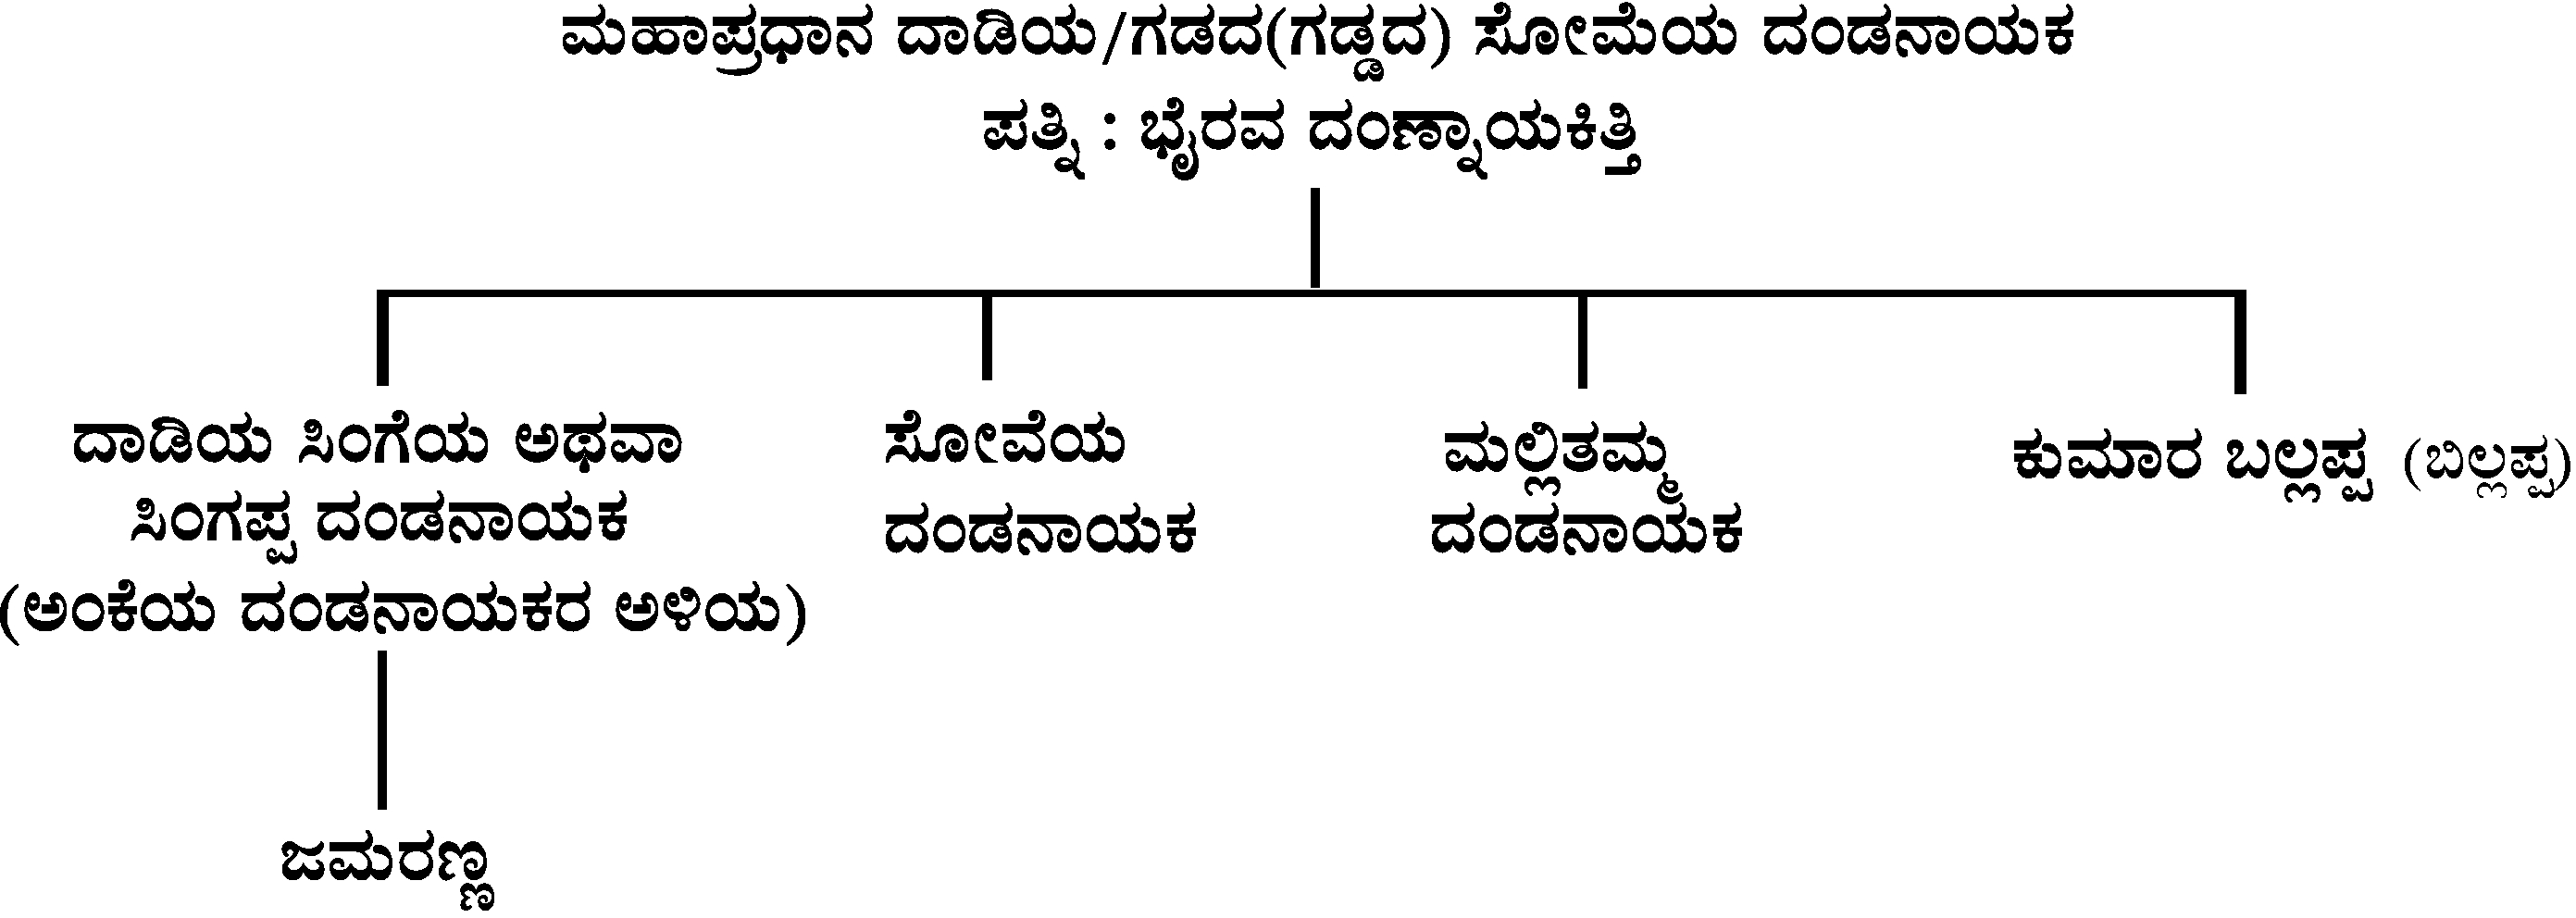
\includegraphics[scale=1.15]{images/chap3/chap3fig25.jpeg}
\end{figure}

\textbf{ಮಹಾಪ್ರಧಾನ\index{ಮಹಾಪ್ರಧಾನ} ಆದಿಸಿಂಗೆಯ ದಂಡನಾಯಕ\index{ಆದಿಸಿಂಗೆಯ ದಂಡನಾಯಕ}(1334):} ಶ‍್ರೀಮನ್​ ಮಹಾಪ್ರಧಾನ ಆದಿಸಿಂಗೆಯ ದಂಡನಾಯಕನು ಮುಮ್ಮಡಿ ಬಲ್ಲಾಳನ ರಾಣಿವಾಸ\index{ರಾಣಿವಾಸ} ದೇಮಲದೇವಿ\index{ದೇಮಲದೇವಿ (ದೇಮಲಾದೇವಿ)}(ದೇವಲದೇವಿ) ಹೆಸರಿನಲ್ಲಿ ಕಲ್ಲಹಳ್ಳಿಯನ್ನು\index{ಕಲ್ಲಹಳ್ಳಿ} ದೇವಲಾಪುರವೆಂಬ\index{ದೇವಲಾಪುರ} ಅಗ್ರಹಾರ\-ವನ್ನಾಗಿ ಮಾಡಿ, ದೇವಲಮಹಾಸಮುದ್ರ\index{ದೇವಲಮಹಾಸಮುದ್ರ} ಕೆರೆಯನ್ನು ಕಟ್ಟಿಸಿ, ಅದನ್ನು ಮಹಾಜನಗಳಿಗೆ ವೀರಬಲ್ಲಾಳನ ಕೈಯಲ್ಲೇ ಧಾರೆಯೆರೆಸಿ ಕೊಡುತ್ತಾನೆ.\endnote{ ಎಕ 6 ಕೃಪೇ 108 ವರಾಹನಾಥ ಕಲ್ಲಹಳ್ಳಿ 1334} ವೀರಬಲ್ಲಾಳನ ರಾಣಿಯ ಹೆಸರನ್ನು ತಿಳಿಸುವ ಶಾಸನ ಇದೊಂದೇ ಆಗಿದೆ. ಇವನೂ ದಾಡಿಯ ಸೋಮೆಯ ದಂಡನಾಯಕನ ಮಗ ಸಿಂಗೆಯದಂಡನಾಯಕನೂ ಅಭಿನ್ನರಿರಬಹುದು.

\textbf{ಮಹಾಪ್ರಧಾನ ಕುಮಾರ ಹೆಗ್ಗಡೆದೇವ ದಂಡನಾಯಕ (14ನೇ ಶ.):} ಶ‍್ರೀಮನ್​ ಮಹಾಪ್ರಧಾನ ಕುಮಾರಹೆಗ್ಗಡೆದೇವ ದಂಡಡನಾಯಕನ ಬಲುಮನುಷ ಬಿಲ್ಲಂಗೆರೆಯ ರಾಮಯ್ಯ, ಬಳ್ಳೆಗೊಳ ಗ್ರಾಮಕ್ಕೆ ಕಾವೇರಿ ನದಿಗೆ ಅಡ್ಡಲಾಗಿ ಕಟ್ಟೇರಿ ಮಡುವನ್ನು ನಿರ್ಮಿಸಿದನೆಂದು ತಿಳಿದುಬರುತ್ತದೆ.\endnote{ ಎಕ 6 ಶ‍್ರೀಪ 84 ಕಾರೇಪುರ 14ನೇ ಶ.} ಕುಮಾರ ಹೆಗ್ಗಡೆದೇವ ದಂಡನಾಯಕನು ಮುಮ್ಮಡಿ ಬಲ್ಲಾಳನ ಕಾಲದಲ್ಲಿಯೇ ಇದ್ದಿರಬಹುದು ಹಾಗೂ ಇವನ ಆಜ್ಞೆಯ ಮೇರೆಗೆ, ಅವನ ಅಧಿಕಾರಿ ರಾಮಯ್ಯ ಕಾವೇರಿ ನದಿಗೆ ಕಟ್ಟೆಯನ್ನು ನಿರ್ಮಿಸಿರಬಹುದು. ಕಟ್ಟೇರಿ ಎಂಬ ಊರು ಕೃಷ್ಣರಾಜಸಾಗರದ ಉತ್ತರ ದಂಡೆಯಲ್ಲಿದೆ.

\vskip .5cm


\section*{ಮಹಾಪ್ರಧಾನ ಸರ್ವಾಧಿಕಾರಿ ಹೆಗ್ಗಡೆಗಳು\index{ಮಹಾಪ್ರಧಾನ ಸರ್ವಾಧಿಕಾರಿ ಹೆಗ್ಗಡೆಗಳು} / ಮಹಾಪ್ರಧಾನ ತಂತ್ರವೆಗ್ಗಡೆ\index{ಮಹಾಪ್ರಧಾನ ತಂತ್ರವೆಗ್ಗಡೆ}/ ದಂಡದಧಿಷ್ಠಾಯಕರು\index{ದಂಡದಧಿಷ್ಠಾಯಕ}/\break ಮಹಾಪಸಾಯ್ತರು\index{ಮಹಾ ಪಸಾಯ್ತ (ಪಸಾಯಿತ, ಪಸಾಯತ)ರು} / ಶ‍್ರೀಕರಣರು\index{ಶ‍್ರೀಕರಣ}}

\vskip .15cm

ಹೊಯ್ಸಳರ ಆಡಳಿತದಲ್ಲಿ ಮಹಾಪ್ರಧಾನ ಸರ್ವಾಧಿಕಾರಿ ಹೆಗ್ಗಡೆಗಳು, ಮಹಾಪ್ರಧಾನ ಹೆಗ್ಗಡೆಗಳು ಹೆಚ್ಚಾಗಿ ಕಾಣಿಸಿಕೊಳ್ಳುತ್ತಾರೆ. ಕೆಲವರು ಮಹಾಪ್ರಧಾನರಾಗಿದ್ದರೂ ದಂಡನಾಯಕರಾಗಲೀ, ಸೇನಾಪತಿಗಳಾಗಲೀ ಆಗಿರಲಿಲ್ಲ. ಆದರೂ ಕೂಡಾ ಇವರು ಮಂತ್ರಿ ಪರಿಷತ್ತಿನಲ್ಲಿ ಸ್ಥಾನಪಡೆದು ಮಹಾಪ್ರಧಾನರೆನಿಸಿಕೊಂಡಿದ್ದರೆಂದು ಹೇಳಬಹುದು. ಮಹಾಪ್ರಧಾನ ಹೆಗ್ಗಡೆಗಳನ್ನು ಶಾಸನಗಳಲ್ಲಿ ಸಚಿವ, ಮಂತ್ರಿ, ಅಮಾತ್ಯ ಎಂದು ಕರೆಯಲಾಗಿದೆ. ಆದರೆ ದಂಡನಾಯಕರೆಂಬ ವಿಶೇಷಣ ಇವರಿಗಿಲ್ಲದಿರುವುದು ಪ್ರಮುಖವಾಗಿ ಗಮನಿಸಬೇಕಾದುದು. ಮಹಾಪ್ರಧಾನ ಹುದ್ದೆಯ ಜೊತೆಗೆ ಇವರು ಸರ್ವಾಧಿಕಾರಿ, ಹಿರಿಯಹೆಗ್ಗಡೆ, ತಂತ್ರವೆಗ್ಗಡೆ, ಮಹಾಪಸಾಯ್ತ, ಶ‍್ರೀಕರಣ ಮೊದಲಾದ ಹುದ್ದೆಗಳನ್ನು ಅಲಂಕರಿಸಿದ್ದರು. ಈ ಹುದ್ದೆಗಳನ್ನು ಹೊಂದಿದ್ದರಿಂದಲೇ ಅವರು ಮಂತ್ರಿ ಪರಿಷತ್ತಿನಲ್ಲಿ ಸ್ಥಾನಪಡೆದು ಮಹಾಪ್ರಧಾನರೆನಿಸಿದ್ದರೆಂದು ಹೇಳಬಹುದು. ಇವರ ಕೈಕೆಳಗೆ ಮಹಾಪ್ರಧಾನ ಹೆಗ್ಗಡೆಗಳು, ವಿವಿಧ ಆಡಳಿತಕ್ಕೆ ಸಂಬಂಧಿಸಿದ ಹೆಗ್ಗಡೆಗಳು ಮೊದಲಾದ ಅಧಿಕಾರಿಗಳಿದ್ದರು.

\vskip 4pt

\textbf{ಮಹಾಪ್ರಧಾನ ತಂತ್ರವೆಗ್ಗಡೆ ದೇವರಾಜ\index{ದೇವರಾಜ} (1145):} ತಂತ್ರವೆಗ್ಗಡೆಯು ರಾಜನ ರಾಜಕೀಯ ತಂತ್ರಗಳ ಆಪ್ತ ಸಮಾಲೋಚಕ\-ರಲ್ಲಿ ಒಬ್ಬನಾಗಿದ್ದು, ಇದೊಂದು ಮುಖ್ಯ ಹುದ್ದೆಯಾಗಿರಬಹುದು.ಮಹಾಪ್ರಧಾನ ತಂತ್ರವೆಗ್ಗಡೆ ಕೌಶಿಕ ಕುಳಾಂಬರ\break ದಿವಾಕರನೆನಿಸಿದ ದೇವರಾಜನನ್ನು \textbf{“ಮಹಾಮಾತ್ಯಪದವೀ\index{ಮಹಾಮಾತ್ಯಪದವೀ} ಪ್ರಖ್ಯಾತಂ, ಶಕ್ತಿತ್ರಯಸಮನ್ವಿತಂ, ಶ‍್ರೀ ವೀರವಿಷ್ಣುವರ್ಧನದೇವ ಸಪ್ತಾಂಗಲಕ್ಷ್ಮೀ ರಕ್ಷಣಾಂಗ ರಕ್ಷಕ, ಅಭಿನವ ಭರತ, ವೀರವಿಷ್ಣುವರ್ಧನದೇವ\index{ವೀರವಿಷ್ಣುವರ್ಧನದೇವ} ಭುಜವಿಜಯ ಮಂಡಿತ ಮಾನವಾಕಾರ ಚಕ್ರ, ಸಮ್ಯಕ್ತ್ವ ರತ್ನಾಕರ”} ಎಂದು ಯಲ್ಲಾದಹಳ್ಳಿ ಶಾಸನವು ಸ್ತುತಿಸುತ್ತದೆ.\endnote{ ಎಕ 7 ನಾಮಂ 64 ಯಲ್ಲಾದಹಳ್ಳಿ 1145} ಹೊಯ್ಸಳ ಮಹೀಭುಜನು(ವಿಷ್ಣುವರ್ಧನ) \textbf{“ಅರ್ಕ್ಕರದುರ್ಕ್ಕೆಯಿಂದ ಕೊಡಲು ಅಶೇಷರಾಜ್ಯಭಾರ ದುರಂಧರನೆಂದು ತಂತ್ರವೆಗ್ಗಡೆತನವನ್ನು ನಿರಂತರವೆನ್ನಲು”} ಪಡೆದನಂತೆ. ರಾಜನು ಅರ್ಹರನ್ನು ಈ ಪದವಿಗೆ ನೇಮಕ ಮಾಡುತ್ತಿದ್ದುದು ಇದರಿಂದ ತಿಳಿಯುತ್ತದೆ. \textbf{“ಪ್ರಭುಶಕ್ತಿಯನಾಂತ ಪೆರ್ಮ್ಮೆ ನೂರ್ಮ್ಮಡಿ ಮಿಗಿಲಾದುದು ಏವೊಗಳ್ವೆನುನ್ನತಿಯಂ ವಿಭು ದೇವರಾಜನಂ” }ಎಂದು ಶಾಸನ ಉದ್ಗಾರವೆತ್ತಿದೆ. ದೇವರಾಜನಿಗೆ ದೇವಣ ಎಂದೂ ಹೆಸರಿತ್ತು. ಈ ಶಾಸನದಲ್ಲಿ ದೇವರಾಜನ ಕುಲ ಹಾಗೂ ಗುರುಪರಂಪರೆಯನ್ನು ನೀಡಿದೆ. ಕೌಶಿಕ ಮುನಿಯಿಂದ ಇವನ ಕುಲಕ್ಕೆ ಕೌಶಿಕ ಕುಲವೆಂಬ ಹೆಸರು ಬಂದಿತು. ಈ ಕುಲದಲ್ಲಿ ದೇವರಾಜನು ಪ್ರಸಿದ್ಧನು. ಅವನ ಹೆಂಡತಿ ಕಾಮಿಕಬ್ಬೆ\index{ಕಾಮಿಕಬ್ಬೆ} ಅಥವಾ ಕಾಮಲದೇವಿ. ಇವರ ಮಗ ಉದಯಾದಿತ್ಯ. ಇವನ ಹೆಂಡತಿ ಕಿರುಗಣಬ್ಬೆ. ಇವರಿಗೆ ರತ್ನತ್ರಯದಂತೆ ದೇವರಾಜ, ಸೋಮನಾಥ ಮತ್ತು ಶ‍್ರೀಧರ ಎಂಬ ಮೂರು ಜನ ಮಕ್ಕಳು. ದೇವರಾಜನು ಸಕುಟುಂಬಸಮೇತನಾಗಿ \textbf{“ಜೈನಧರ್ಮನಿರ್ಮಳಾಂಬರ ಮಹೀಕರನೂ, ಹೊಯ್ಸಳಮಹೀಶ ರಾಜ್ಯ ಭೂಭ್ರುನ್ನಿಳಯ ಮಣಿಪ್ರದೀಪ ಕಳಶನೂ”} ಆಗಿದ್ದಾಗ, ಹೊಯ್ಸಳನು ಅಂದರೆ ವಿಷ್ಣುವರ್ಧನನು ದೇವರಾಜನ ಧರ್ಮಬುದ್ಧಿ ಮತ್ತು ಸ್ವಾಮಿಭಕ್ತಿಗೆ ಮೆಚ್ಚಿ, ಅವನಿಗೆ ಸೂರನಹಳ್ಳಿಯನ್ನು\index{ಸೂರನಹಳ್ಳಿ}(ಮೆಚ್ಚುಗೆಯಾಗಿ) ಕೊಟ್ಟನು. ದೇವರಾಜನು ಅದನ್ನು ಪಾರ್ಶ್ವಪುರವನ್ನಾಗಿ\index{ಪಾರ್ಶ್ವಪುರ} ಮಾಡಿ, ಅಲ್ಲಿ \textbf{“ರಾಜ ರಾಷ್ಟ್ರ ಯಶೋಧನ ವೃದ್ಧ್ಯರ್ತ್ಥವಾಗಿ” }ಅಮರೇಂದ್ರ ಭವನದಂತಿದ್ದ ಪಾರ್ಶ್ವನಾಥ ತ್ರಿಕೂಟ ಜಿನಾಲಯವನ್ನು ಕಟ್ಟಿಸಿ, ಪಾರ್ಶ್ವನಾಥ ದೇವರ ಅರ್ಚನೆಗೆ ಸೂರನಹಳ್ಳಿಯ ಮೊದಲ ನಾಲ್ವತ್ತು ಹೊನ್ನೊಳಗೆ ಹತ್ತು ಹೊನ್ನನ್ನು, ತನ್ನ ಗುರು ಮುನಿಚಂದ್ರ ದೇವರ\index{ಮುನಿಚಂದ್ರ ದೇವರು} ಶ‍್ರೀಪಾದವನ್ನು ತೊಳೆದು ದತ್ತಿಯಾಗಿ ಬಿಟ್ಟನು. ಹಾಗೂ ಆ ಊರಿನ ದೇವರ ಕೆರೆಯ ಕೆಳಗೆ ಗದ್ದೆ ಬೆದ್ದಲುಗಳನ್ನು ದತ್ತಿಯಾಗಿ ಬಿಟ್ಟನು. ಶಾಸನದಲ್ಲಿ ನೀಡಿರುವ ಈತನ ವಂಶವೃಕ್ಷ ಈ ಕೆಳಗಿನಂತಿದೆ. ಆದರೆ ಮುಂದೆ ಯಾವುದೇ ಶಾಸನದಲ್ಲೂ ಕೂಡಾ ಈ ವಂಶದ ಉಲ್ಲೇಖ ಕಂಡುಬರುವುದಿಲ್ಲ. ಈ ಶಾಸನವು ಈಗ ಬೆಳ್ಳೂರು\index{ಬೆಳ್ಳೂರು} ಬಸದಿಯಲ್ಲಿದೆ. ಸೂರನಹಳ್ಳಿಯ ಪಕ್ಕದಲ್ಲಿಯೇ ಯಲಾದಹಳ್ಳಿ\index{ಯಲಾದಹಳ್ಳಿ (ಯಲ್ಲಾದಹಳ್ಳಿ)} ಇದೆ. ಈ ಎರಡೂ ಊರಿಗೆ ಮಧ್ಯದಲ್ಲಿ ಎತ್ತರವಾದ ಗುಡ್ಡದ ಮೇಲಿರುವ ತ್ರಿಕೂಟ ಬಸದಿಯು ಜೀರ್ಣವಾಗಿದೆ. ಇದನ್ನು ಮೂಲ ರೂಪದಲ್ಲಿ ಪುನರ್ ನಿರ್ಮಿಸಿದಲ್ಲಿ ಜಿಲ್ಲೆಯ ಅತ್ಯಂತ ಸುಂದರವಾದ ಬಸದಿಗಳಲ್ಲಿ ಒಂದಾಗುತ್ತದೆ. ದೇವರಾಜನ ವಂಶಾವಳಿ ಈ ಕೆಳಗಿನಂತಿದೆ.

\begin{figure}[H]
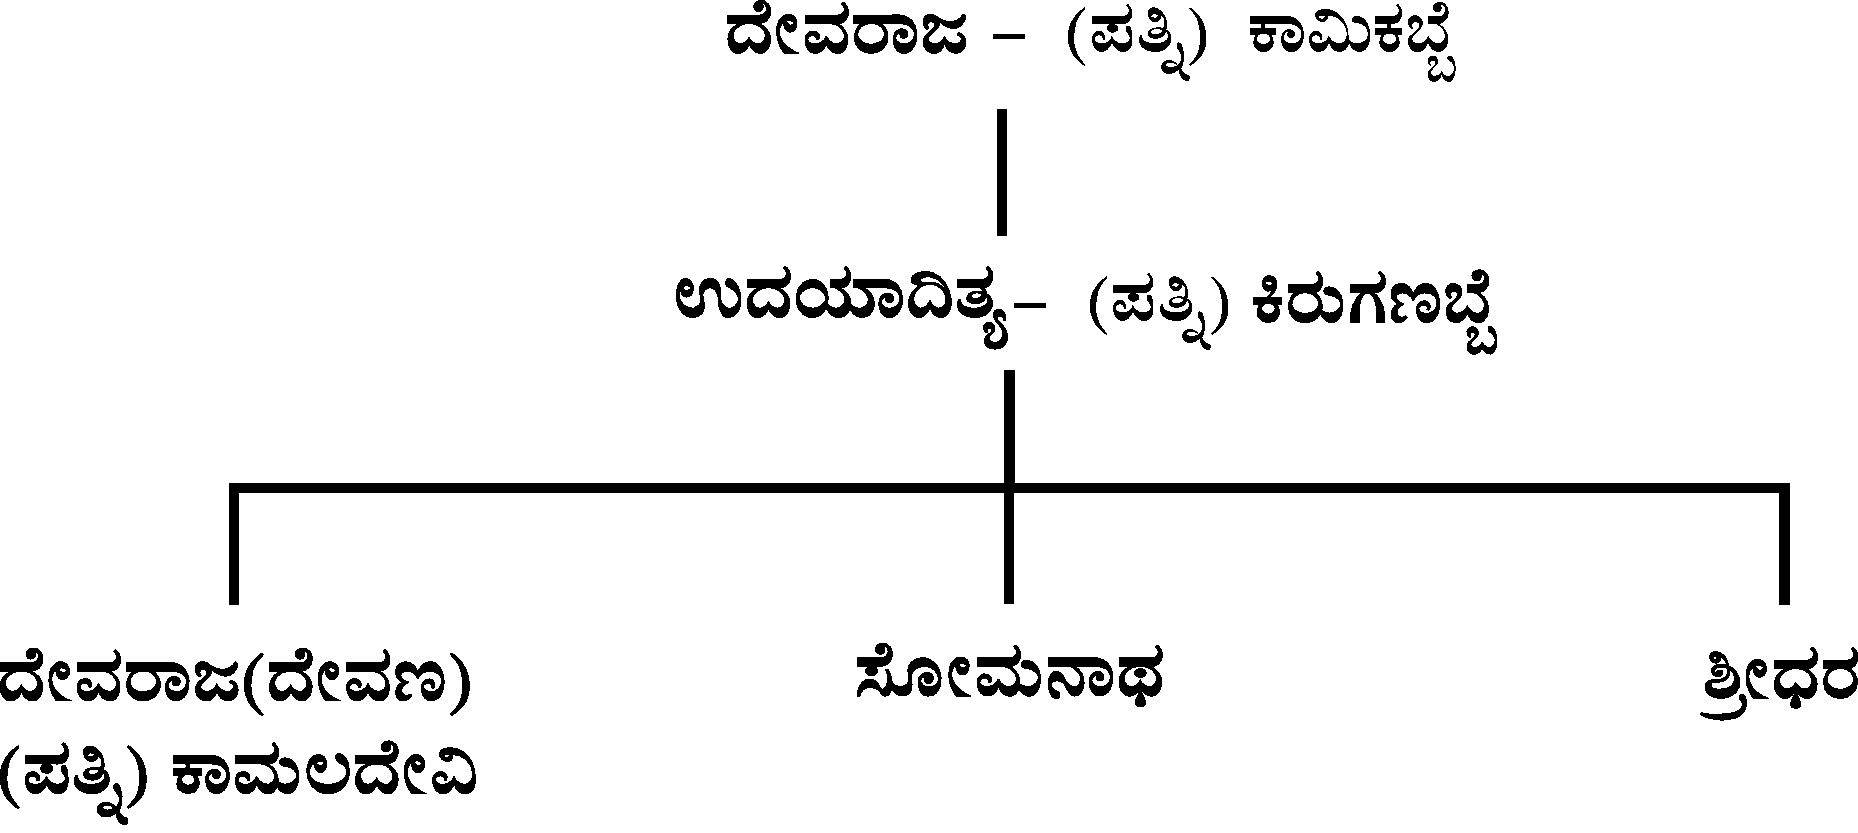
\includegraphics[scale=1.15]{images/chap3/chap3fig15.jpeg}
\end{figure}

\textbf{ಮಹಾಪ್ರಧಾನ ಸರ್ವಾಧಿಕಾರಿ ಹೆಗ್ಗಡೆ\index{ಮಹಾಪ್ರಧಾನ ಸರ್ವಾಧಿಕಾರಿ ಹೆಗ್ಗಡೆ} ವಿಭು ಬಲ್ಲಯ್ಯ\index{ಬಲ್ಲಯ್ಯ} (1144\general{\enginline{-}}1174):} ಶ‍್ರೀಮನ್ಮಹಾಪ್ರಧಾನ ಸರ್ವಾಧಿಕಾರಿ ಹೆಗ್ಗಡೆ ಬಲ್ಲಯ್ಯನು \textbf{“ಬಲ್ಲಾಳಮಹೀಕಾಂತನ ವರಮಂತ್ರಿವಲ್ಲಭ”} ನಾಗಿದ್ದನೆಂದು ಬೋಗಾದಿ\index{ಬೋಗಾದಿ} ಶಾಸನದಿಂದ ತಿಳಿದುಬರುತ್ತದೆ.\endnote{ ಎಕ 7 ನಾಮಂ 184 ಬೋಗಾದಿ 1173} ಭೋಗವದಿಯ(ಬೋಗಾದಿ) ಶ‍್ರೀಕರಣದ ಜಿನಾಲಯದ, ಪಾರ್ಶ್ವದೇವರ\index{ಪಾರ್ಶ್ವದೇವರು} ಅಷ್ಟವಿಧಾರ್ಚನೆಗೆ, ಕಾಳಬೋವನಹಳ್ಳಿಯನ್ನು ಮತ್ತು ಬೋಗವದಿಯ\index{ಬೋಗವದಿ} ಸಮಸ್ತ ಸುಂಕವನ್ನು \textbf{“ಮನಮೊಸೆದು ಭೋಗವಸದಿಯೊಳು ಜಿನಪೂಜೆಗೆ”} ದತ್ತಿಯಾಗಿ ಬಿಡುತ್ತಾನೆ. ಈ ಬಸದಿಯನ್ನು ಕ್ರಿ.ಶ.1144ರಲ್ಲಿ, ವಿಷ್ಣುವರ್ಧನನ ಕಾಲದಲ್ಲಿ ವೋಣಮಯ್ಯನ ಮಗ ಶ‍್ರೀಕರಣದ ಮಾಧವ\index{ಶ‍್ರೀಕರಣದ ಮಾಧವ} ಅಥವಾ ಮಾದಿರಾಜನು\index{ಮಾದಿರಾಜ} ಕಟ್ಟಿಸಿರಬಹುದು.\endnote{ ಎಕ 7 ನಾಮಂ 183 ಬೋಗಾದಿ 1144} ಕ್ರಿ.ಶ.1173ರಲ್ಲಿ, ಈ ಶ‍್ರೀಕರಣ ಜಿನಾಲಯವನ್ನು ವಿಭು ಮಾಚಿರಾಜನು ಜೀರ್ಣೋದ್ಧಾರ ಮಾಡಿ, ಅವನ ಮಾವ ಮಹಾಪ್ರಧಾನ ಸರ್ವಾಧಿಕಾರಿ ಬಲ್ಲಯ್ಯನ ಹಸ್ತದಿಂದ ದತ್ತಿಗಳನ್ನು ಬಿಡಿಸಿದ್ದಾನೆಂದು ಹೇಳಬಹುದು. ಬೋಗಾದಿ ಶಾಸನದಲ್ಲಿರುವ ಮಾಚಿರಾಜನ ಸ್ತುತಿ ಹೀಗಿದೆ.\endnote{ ಎಕ 7 ನಾಮಂ 184 ಬೋಗಾದಿ 1173}

\begin{verse}
\textbf{ಮಹಾಂಗಮಂತ್ರ ಕಮನೀಯಾ} \\\textbf{ ಳಂಬಿತ ಸುರರಾಜಪೂಜ್ಯ ಚರಣಾಕ್ಯನೆನಲು} \\\textbf{ ಸಂಚಿತ ಕೀರ್ತಿ ಪರಾಕ್ರಮ}\\\textbf{ ಪ್ರಭಾವನೆನಿಸಿ ಮಾಚಿರಾಜಂ ನೆಗಳ್ದಂ}
\end{verse}

\begin{verse}
\textbf{ಆ ವಿಭು ಮಾಚಿರಾಜನ} \\\textbf{ ಮಾವಂ ಬಲ್ಲಯ್ಯನಯ್ಯನೀ ಧರೆಗೆಲ್ಲಂ} \\\textbf{ಕಾವ ಗುಣದಿನಾದನದಾವಂ} \\\textbf{ ಗುಣಗಣದಿನಾತನೆಣೆಯಪ್ಪಂನಂ}
\end{verse}

ಅರಸಾದಿತ್ಯ\index{ಅರಸಾದಿತ್ಯ} ಮತ್ತು ಆಚಾಂಬಿಕೆಗೆ\index{ಆಚಾಂಬಿಕೆ} ಪಂಪರಾಜ\index{ಪಂಪರಾಜ}, ಹರಿದೇವ\index{ಹರಿದೇವ} ಮತ್ತು ಮಂತ್ರಿಯೂಥಾಗ್ರಣಿ ಬಲದೇವಣ್ಣ (ಬಲ್ಲಯ್ಯ)\index{ಬಲದೇವಣ್ಣ (ಬಲ್ಲಯ್ಯ)} ಎಂಬ ಮೂವರು ಮಕ್ಕಳಿದ್ದರೆಂದು, ಇವರು ಕರ್ನಾಟಕ ಕುಳತಿಳಕ ಮಾಚಿರಾಜಂಗೆ ಮಾವಂದಿರಾಗಿದ್ದರೆಂದು ಶ್ರವಣಬೆಳಗೊಳದ ದೊಡ್ಡಬೆಟ್ಟದ ಅಷ್ಟದಿಕ್ಪಾಲಕರ ಮಂಟಪದ ಶಾಸನದಿಂದ ತಿಳಿದುಬರುತ್ತದೆ.\endnote{ ಎಕ 2 ಶ್ರಬೆ 322 ದೊಡ್ಡಬೆಟ್ಟ 12ನೇ ಶ.} ಹರಿದೇವ, ಹಂಪರಾಜರ ಅನುಜನಾದ ಸಚಿವ ಬಲದೇವನು \textbf{“ಕರಮೆಸೆಯೆ ಗೊಂಮಟೇಶ್ವರ ಮಾನಸ್ತಂಭ\index{ಗೊಂಮಟೇಶ್ವರ ಮಾನಸ್ತಂಭ} ಯಕ್ಷನಂ ಮಾಡಿಸಿದಂ”} ಎಂದು ಶ್ರವಣಬೆಳಗೊಳ\index{ಶ್ರವಣಬೆಳಗೊಳ} ದೊಡ್ಡಬೆಟ್ಟದ ಮಾನಸ್ತಂಭದ ಶಾಸನದಿಂದ ತಿಳಿದುಬರುತ್ತದೆ.\endnote{ ಎಕ 2 ಶ್ರಬೆ 359 ಚಿಕ್ಕಬೆಟ್ಟ 12ನೇ ಶ.} ಈ ಮೂವರೂ ಸಹೋದರರಾಗಿದ್ದರೆಂಬುದು ಇದರಿಂದ ಖಚಿತವಾಗುತ್ತದೆ.

ಶ‍್ರೀಪಾಲ ಯೋಗೀಂದ್ರರ\index{ಶ‍್ರೀಪಾಲ ಯೋಗೀಂದ್ರ} ಶಿಷ್ಯ ವಾದಿರಾಜದೇವನ\index{ವಾದಿರಾಜದೇವ} ಸಲ್ಯದ\index{ಸಲ್ಯ (ಚಲ್ಯ)}(ಚಲ್ಯ) ಕುಂಬೇನಹಳ್ಳಿಯಲ್ಲಿ\index{ಕುಂಬೇನಹಳ್ಳಿ} ತಮ್ಮ ಗುರುಗಳಿಗೆ ಪರೋಕ್ಷ ವಿನಯವಾಗಿ, ಪರವಾದಿಮಲ್ಲ ಜಿನಾಲಯವನ್ನು ನಿರ್ಮಿಸಿದಾಗ, ಅದಕ್ಕೆ ಶ‍್ರೀಮನ್​ಮಹಾಪ್ರಧಾನ ಸರ್ವಾಧಿಕಾರಿ\break ತಂತ್ರಾಧಿಷ್ಠಾಯಕ ಕಮ್ಮಟದ ಮಾಚಯ್ಯನು, ಮಾವ ಬಲ್ಲಯ್ಯನು, ಗಾಣದ ಸುಂಕವನ್ನು\index{ಗಾಣದ ಸುಂಕ} ಬಿಡುತ್ತಾರೆ. ಕುಂಬೇನಹಳ್ಳಿಯು\index{ಕುಂಬೇನಹಳ್ಳಿ} ನಾಗಮಂಗಲ ತಾಲ್ಲೂಕಿನ ಗಡಿಯಲ್ಲಿರುವ ಶ್ರವಣಬೆಳಗೊಳಕ್ಕೆ ಸಮೀಪವಿರುವ ಹಳ್ಳಿಯಾಗಿದೆ. ಇಲ್ಲಿನ ಬಸದಿಯು ಬಿದ್ದುಹೋಗಿ, ಆಂಜನೇಯನ ಗುಡಿಯಾಗಿ ಪರಿವರ್ತಿತವಾಗಿದೆ. ಶಾಸನೋಕ್ತ ಮಾವ ಬಲ್ಲಯ್ಯ, ಹರಿಹರ, ಹಂಪರಾಜರ ತಮ್ಮ ಬಲ್ಲಯ್ಯನೇ ಆಗಿದ್ದಾನೆ.\endnote{ ಎಕ 2 ಶ್ರಬೆ 572 ಕುಂಬೇನಹಳ್ಳಿ 12ನೇ ಶ.}

ಇವರೇ ಬೋಗಾದಿ ಶಾಸನೋಕ್ತ ಬಲ್ಲಯ್ಯ\index{ಬಲ್ಲಯ್ಯ} ಮತ್ತು ಮಾಚಿರಾಜರಾಗಿದ್ದಾರೆಂದು\index{ಮಾಚಿರಾಜ} ಊಹಿಸಬಹುದು. ಮಾಚಿರಾಜನು ಆಚಾಂಬಿಕೆಯ ಸೋದರನಾಗಿರಬಹುದು. ಮೊದಲು ಇವರು ಕರ್ನಾಟಕ ಬ್ರಾಹ್ಮಣ ವಂಶಕ್ಕೆ ಸೇರಿದ್ದು, ನಂತರ ಜೈನಧರ್ಮವನ್ನು ಸ್ವೀಕರಿಸಿರಬಹುದು. ಈ ಭಾಗದ ಹಳ್ಳಿಯ ಜನರು ಬಲ್ಲೇಗೌಡ, ಬಲ್ಲಪ್ಪ, ಬಲ್ಲಯ್ಯ ಎಂದು ಇತ್ತೀಚಿನವರೆಗೂ ಹೆಸರಿಟ್ಟು\-ಕೊಳ್ಳುತ್ತಿದ್ದರು.

\textbf{ಮಹಾಪ್ರಧಾನ ದಂಡದಧಿಷ್ಠಾಯಕ\index{ದಂಡದಧಿಷ್ಠಾಯಕ} ಮಹಾಪಸಾಯ್ತ\index{ಮಹಾ ಪಸಾಯ್ತ (ಪಸಾಯಿತ, ಪಸಾಯತ)ರು} ಹಿರಿಯ ಹೆಗ್ಗಡೆ ಮಾಚಯ್ಯ\index{ಮಾಚಯ್ಯ} ಮತ್ತು ಶ‍್ರೀಮನ್ಮಹಾಪ್ರಧಾನ ಸರ್ವಾಧಿಕಾರಿ\index{ಶ‍್ರೀಮನ್ಮಹಾಪ್ರಧಾನ ಸರ್ವಾಧಿಕಾರಿ} ದಂಡನಾಯಕ ಕೇಶಿಯಣ್ಣ\index{ಕೇಶಿಯಣ್ಣ} (1173\general{\enginline{-}}74):} ಶ‍್ರೀಮನ್​ಮಹಾಪ್ರಧಾನ, ಸರ್ವಾಧಿಕಾರಿ, ದಂಡದಧಿಷ್ಠಾಯಕ, ಮಹಾಪಸಾಯ್ತ\index{ಮಹಾ ಪಸಾಯ್ತ (ಪಸಾಯಿತ, ಪಸಾಯತ)ರು}, ಹಿರಿಯಹೆಗ್ಗಡೆ ಮಾಚಯ್ಯನು, ಇಮ್ಮಡಿ ವೀರ ಬಲ್ಲಾಳನ ಕಾಲದಲ್ಲಿದ್ದನು. ಇವನು ಮತ್ತು ಇವನ ಮಕ್ಕಳಾದ ಹೆಗ್ಗಡೆ ಕೇಶಿಯಣ್ಣ\index{ಹೆಗ್ಗಡೆ ಕೇಶಿಯಣ್ಣ} ಮತ್ತು ಹೆಗ್ಗಡೆ ಕೊಮ್ಮಣ್ಣ\index{ಹೆಗ್ಗಡೆ ಕೊಮ್ಮಣ್ಣ} ಇವರುಗಳು ಯಾದವನಾರಾಯಣ ಚತುರ್ವೇದಿಮಂಗಲದ\index{ಯಾದವನಾರಾಯಣ ಚತುರ್ವೇದಿ} ಅಂದರೆ ತೊಂಡನೂರಿನ ಶ‍್ರೀ ಲಕ್ಷ್ಮೀನಾರಾಯಣ ದೇವರಿಗೆ ದತ್ತಿಗಳನ್ನು ಬಿಟ್ಟಿದ್ದಾರೆ.\endnote{ ಎಕ 6 ಪಾಂಪು 63 ತೊಣ್ಣೂರು 1174} ಒಬ್ಬ ಅಧಿಕಾರಿಗೇ ಇಷ್ಟೊಂದು ಹುದ್ದೆಗಳನ್ನು ಇವನ ದಕ್ಷ ಕಾರ್ಯನಿರ್ವಹಣೆಯ ಮೇಲೆ ನೀಡಿರಬಹುದು. ಇವನ ಹಿರಿಯ ಮಗ ಹೆಗ್ಗಡೆ ಕೇಶಿಯಣ್ಣನು ಮೊದಲಿಗೆ ಹೆಗ್ಗಡೆ ಪದವಿಯನ್ನು ಹೊಂದಿದ್ದು, ಮೂರು ವರ್ಷಗಳ ನಂತರ ಬಹುಶಃ ಇವನ ತಂದೆಯ ನಂತರ, ಮಹಾಪ್ರಧಾನ ಸರ್ವಾಧಿಕಾರಿ ಹುದ್ದೆಗೆ ಏರಿದ್ದಾನೆ. ಮಾಚಯ್ಯನ ಮಕ್ಕಳಾದ ಶ‍್ರೀಮನ್​ ಮಹಾಪ್ರಧಾನ ಸರ್ವಾಧಿಕಾರಿ ದಂಡನಾಯಕ ಹೆಗ್ಗಡೆ ಕೇಶಿಯಣ್ಣ, ಹೆಗ್ಗಡೆ ಕೊಮ್ಮಣ್ಣ ಮತ್ತು ಹೆಗ್ಗಡೆ ಮಹದೇವಣ್ಣ\index{ಹೆಗ್ಗಡೆ ಮಹದೇವಣ್ಣ} ಇವರುಗಳು ಒಟ್ಟಾಗಿ ಇದೇ ತೊಂಡನೂರಿನ\index{ತೊಂಡನೂರು} ವಿರ್ರಿರುಂದ ಪೆರುಮಾಳೆ ದೇವರಿಗೆ ಬೋಗನಹಳ್ಳಿಯನ್ನು ದತ್ತಿಯಾಗಿ ಬಿಡುತ್ತಾರೆ.\endnote{ ಎಕ 6 ಪಾಂಪು 80 ತೊಣ್ಣೂರು 1177}

\begin{figure}[H]
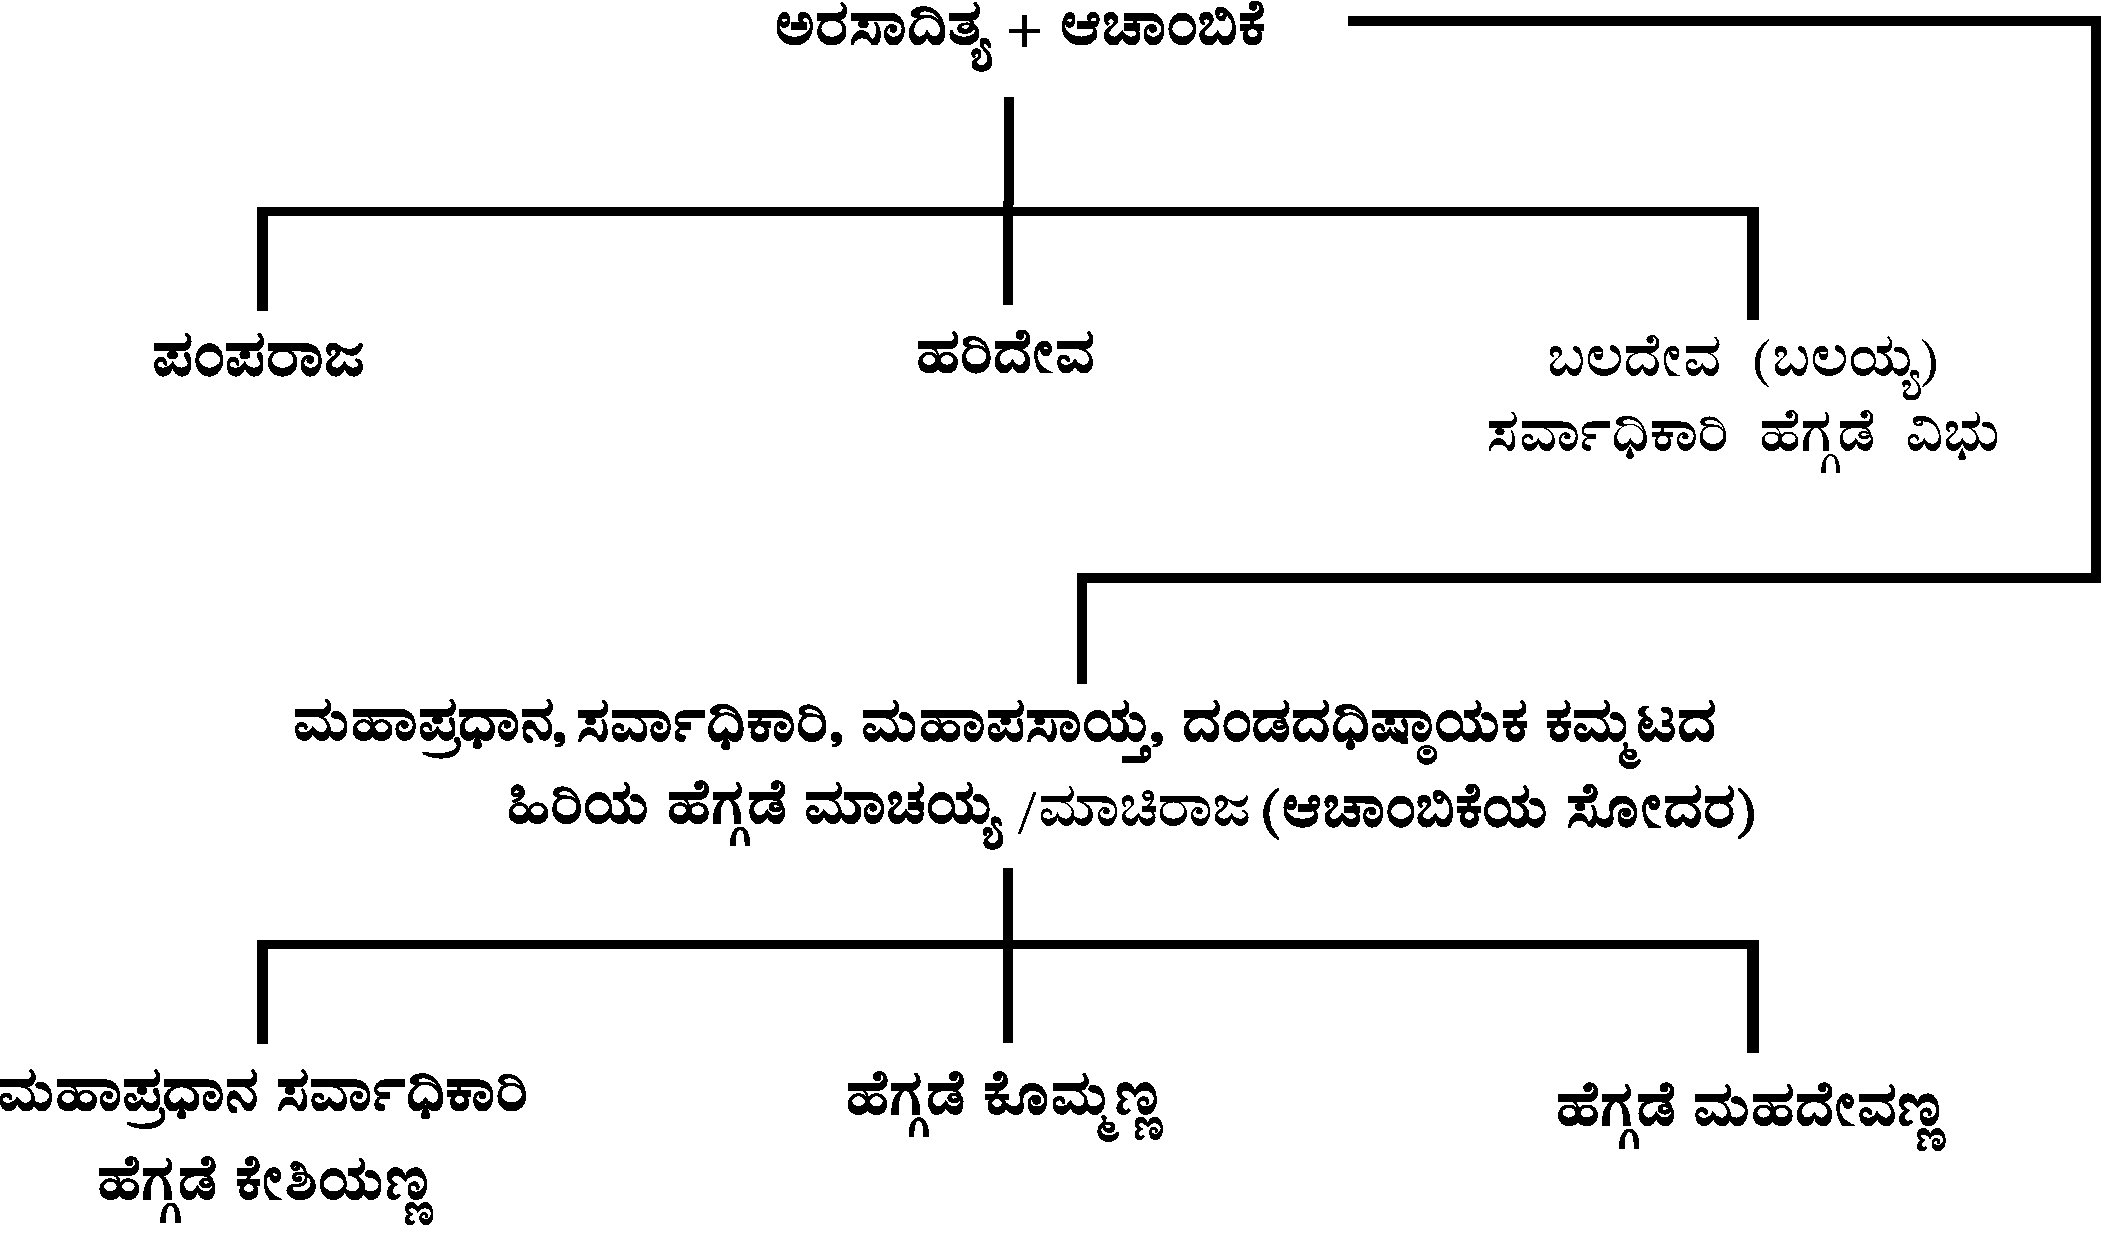
\includegraphics[scale=1.25]{images/chap3/chap3fig26.jpeg}
\end{figure}

ಆನೆಕೆರೆ ಶಾಸನೋಕ್ತ ಮಾಚಿರಾಜನೂ, ತೊಣ್ಣೂರು\index{ತೊಣ್ಣೂರು} ಶಾಸನೋಕ್ತ ಮಾಚಿರಾಜನೂ, ಶ್ರವಣಬೆಳಗೊಳ ಶಾಸನೋಕ್ತ ಮಾಚಿರಾಜನೂ ಅಭಿನ್ನರೆಂದು ಹೇಳಬಹುದು. ಶ್ರವಣಬೆಳಗೊಳಶಾಸನದಲ್ಲಿ ಅರಸಾದಿತ್ಯ ಮತ್ತು ಆಚಾಂಬಿಕೆಯ ಮಕ್ಕಳಾದ ಪಂಪರಾಜ, ಹರಿದೇವ ಮತ್ತು ಮಂತ್ರಿ ಬಲದೇವಣ್ಣ ಇವರು ಕರ್ನಾಟಕ ಕುಲತಿಲಕ ಮಾಚಿರಾಜನ ಮಾವಂದಿರೆಂದು ಹೇಳಿದೆ.\endnote{ ಎಕ 2 ಶ್ರಬೆ 322 ದೊಡ್ಡಬೆಟ್ಟ 12ನೇ ಶ.} ಚನ್ನರಾಯಪಟ್ಟಣ,\endnote{ ಎಕ 10 ಚರಾಪ 9 ಚರಾಪ 1181} ಆನೆಕೆರ,\endnote{ ಎಕ 10 ಚರಾಪ 33 ಆನೆಕೆರೆ 1189} ಶಾಸನೋಕ್ತ ಮಾಚಿರಾಜನು ಕರ್ನಾಟಕ ಕುಲ ತಿಲಕನಾಗಿದ್ದಾನೆ\index{ಕರ್ನಾಟಕ ಕುಲ ತಿಲಕ}. ಈ ಶಾಸನಗಳಲ್ಲಿ ಮಾಚಿರಾಜನನ್ನು ಶ‍್ರೀಮನ್​ ಮಹಾಪ್ರಧಾನ ಶ‍್ರೀಕರಣಾಧಿಪತಿ\index{ಶ‍್ರೀಕರಣಾಧಿಪತಿ} ಹಿರಿಯದಂಡನಾಯಕ\index{ಹಿರಿಯದಂಡನಾಯಕ} ಹೆಗ್ಗಡೆ ಮಾಚಯ್ಯ, ಶ‍್ರೀಕರಣದ ಪ್ರೌಢ ಪ್ರಧಾನ\index{ಪ್ರೌಢ ಪ್ರಧಾನ} ಮಾಚಿರಾಜ ಎಂದು ಕರೆದಿದೆ. ಕ್ರಿ.ಶ.1173ರ ಮರ್ಕುಲಿ ಶಾಸನವು ಕಮ್ಮಟದ ಮಾಚಯ್ಯನನ್ನು ಉಲ್ಲೇಖಿಸಿದೆ.\endnote{ ಎಕ 8 ಹಾಸನ 174 ಮರ್ಕುಲಿ 1173} ಬಹುಶಃ ಮಾಚಯ್ಯನು\index{ಮಾಚಯ್ಯ} ಮೊದಲು ಕಮ್ಮಟದ ಮುಖ್ಯಸ್ಥನಾಗಿದ್ದು, ಒಂದು ವರ್ಷದ ಅವಧಿಯಲ್ಲಿ ಅಂದರೆ ಕ್ರಿ.ಶ.1174ರ ವೇಳೆಗೆ ಮಹಾಪ್ರಧಾನನ ಹುದ್ದೆಗೆ ಏರಿರಬಹುದು. ಈ ಎಲ್ಲ ಶಾಸನಗಳೂ ಒಂದೇ ಕಾಲಕ್ಕೆ ಸೇರಿರುವುದರಿಂದ, ಒಂದೇ ಪ್ರದೇಶದಲ್ಲಿರುವುದರಿಂದ ಈ ಶಾಸನಗಳಲ್ಲಿ ಉಕ್ತರಾಗಿರುವ ಮಾಚಿರಾಜರೆಲ್ಲರೂ ಅಭಿನ್ನರೆಂದು (ಒಬ್ಬರೇ) ಹೇಳಬಹುದು. ಇವರ ವಂಶವೃಕ್ಷವನ್ನು ಈ ಮೇಲಿನ ರೀತಿ ಕಟ್ಟಿಕೊಡಬಹುದು.

\textbf{ಮಹಾಪ್ರಧಾನ ಸರ್ವಾಧಿಕಾರಿ\index{ಸರ್ವಾಧಿಕಾರಿ} ಮಹಾಪಸಾಯ್ತ\index{ಮಹಾ ಪಸಾಯ್ತ (ಪಸಾಯಿತ, ಪಸಾಯತ)ರು} ಶ‍್ರೀಕರಣದ ಹೆಗ್ಗಡೆ\index{ಶ‍್ರೀಕರಣದ ಹೆಗ್ಗಡೆ} ಎರೆಯಣ್ಣ\index{ಎರೆಯಣ್ಣ}(1175):} ಇಮ್ಮಡಿ ಬಲ್ಲಾಳನ ಕಾಲದಲ್ಲಿ, ಮಹಾಪ್ರಧಾನ ಸರ್ವಾಧಿಕಾರಿ, ಮಹಾಪಸಾಯ್ತ, ಶ‍್ರೀಕರಣದ ಹೆಗ್ಗಡೆಯಾಗಿದ್ದ ಎರೆಯಣ್ಣನ ಕೈಯಲ್ಲಿ, ಶ‍್ರೀಕರಣದ ಹೆಗ್ಗಡೆ ಕಲಿಯಣ್ಣನು, ಯಾದವನಾರಾಯಣ ಚತುರ್ವೇದಿ ಮಂಗಲದಲ್ಲಿ ಒಂಬತ್ತು ವೃತ್ತಿಗಳನ್ನು ಕ್ರಯದಾನವಾಗಿ ಕೊಂಡು ಅದನ್ನು ಕಾಂಚೀಪುರದ ಅಲ್ಲಾಳಪೆರುಮಾಳ ದೇವರಿಗೆ ದತ್ತಿಯಾಗಿ ಬಿಟ್ಟನು.\endnote{ ಎಕ 6 ಪಾಂಪು 64 ತೊಣ್ಣೂರು 1175} ಮಹಾಪ್ರಧಾನ ಸರ್ವಾಧಿಕಾರಿಗಳು ಪಟ್ಟಣಗಳಲ್ಲಿ ಅಗ್ರಹಾರಗಳಲ್ಲಿ ಈ ರೀತಿಯ ವೃತ್ತಿಗಳ ಒಡೆತನ ಹೊಂದಿದ್ದರೆಂದು ಇದರಿಂದ ತಿಳಿಯಬಹುದು ಹಾಗೂ ಅನೇಕ ಶ‍್ರೀಕರಣದ ಹೆಗ್ಗಡೆಗಳು ಇವರಿಗೆ ಅಧೀನರಾಗಿ ಕೆಲಸ ಮಾಡುತ್ತಿದ್ದರೆಂದು ಹೇಳಬಹುದು.

\textbf{ಶ‍್ರೀಮನ್​ ಮಹಾಪ್ರಧಾನ ಶ‍್ರೀಕರಣದ ಹೆಗ್ಗಡೆ ನಾಗಣ್ಣ\index{ಶ‍್ರೀಕರಣದ ಹೆಗ್ಗಡೆ ನಾಗಣ್ಣ}:} ಇವನೂ ವೀರಬಲ್ಲಾಳನ ಕಾಲದಲ್ಲಿ ತೊಂಡನೂರಿನ\break ಲಕ್ಷ್ಮೀನಾರಾಯಣ ದೇವಾಲಯದ ಮಂಟಪವನ್ನು(ರಂಗಮಂಟಪ) ಕಟ್ಟಿಸಿದನು.\endnote{ ಎಕ 6 ಪಾಂಪು 58 ತೊಣ್ಣೂರು 12ನೇ ಶ.}

\textbf{ಮಹಾಪ್ರಧಾನ ಭದ್ರಕಾಳಿಯಣ್ಣ\index{ಮಹಾಪ್ರಧಾನ ಭದ್ರಕಾಳಿಯಣ್ಣ} ಮತ್ತು ವಾಸುದೇವ\index{ವಾಸುದೇವ} (1177):} ಇಮ್ಮಡಿ ಬಲ್ಲಾಳನ ಕಾಲದಲ್ಲಿ ಕೆಳಲೆನಾಡ ಹುಲ್ಲವಂಗಲದ ಹುಳ್ಳೆಯಹಳ್ಳಿಯಲ್ಲಿ ನಡೆದ ತುರುಗೋಳಿನಲ್ಲಿ ನಾಗೊಡೆಯನು ಸ್ವರ್ಗಸ್ಥನಾದಾಗ, \textbf{ಮಹಾಪ್ರಧಾನ\general{\break } ಭದ್ರಕಾಳಿಯಣ್ಣ ಮತ್ತು ವಾಸುದೇವ} ಇವರುಗಳು, ತಮ್ಮ ಮಾಣಿ (ಶಿಷ್ಯ) ನಾಗೊಡೆಯನಿಗೆ ಗದ್ದೆಯನ್ನು ದತ್ತಿಯಾಗಿ ಬಿಡುತ್ತಾರೆ.\endnote{ ಎಕ 7 ಮವ 39 ಹುಲ್ಲೇಗಾಲ 1178} ಇವರು ಕೆಳಲೆನಾಡಿನ ಆಡಳಿತವನ್ನು ನೋಡಿಕೊಳ್ಳುತ್ತಿದ್ದರೆಂದು ಹೇಳಬಹುದು.

\textbf{ಅಮಾತ್ಯ ಭೀಮೆಯ ನಾಯಕ\index{ಅಮಾತ್ಯ ಭೀಮೆಯ ನಾಯಕ} (1145):} ಹೊಸಹೊಳಲಿನ ಒಂದನೆಯ ನರಸಿಂಹನ ಕಾಲದ, ಎರಡು ತ್ರುಟಿತ ವೀರಗಲ್ಲುಗಳಲ್ಲಿ ಉಲ್ಲೇಖಿತನಾದ,\textbf{ ಭೀಮೆಯನಾಯಕನು\index{ಭೀಮೆಯ ನಾಯಕ} ಸಮಸ್ತ ರಾಜ್ಯಭರ ನಿರೂಪಿತ\index{ಸಮಸ್ತ ರಾಜ್ಯಭರ ನಿರೂಪಿತ} ಅಮಾತ್ಯಪದ\index{ಅಮಾತ್ಯಪದ} (ವಿ)ರಾಜಿತನಾಗಿದ್ದನೆಂದು ತಿಳಿದುಬರುತ್ತದೆ.\endnote{ ಎಕ 6 ಕೃಪೇ 6 ಮತ್ತು 9 ಹೊಸಹೊಳಲು, 12ನೇ ಶ.}}ಇವನು ದಂಡನಾಯಕನೂ, ಮಹಾಪ್ರಧಾನ ಆಗಿರಬಹುದು. ಇವನ ನೇತೃತ್ವದಲ್ಲಿ ನಡೆದ ಯುದ್ಧದಲ್ಲಿ ಹರಿದೇವ, ಅವನ ಮಗ ಸೋಮೆಯಜ, ಅವನ ಮಯ್ದುನ ಮಸಣೆಯ ನಾಯಕ ಇವರು ಸತ್ತರೆಂದು ತಿಳಿದುಬರುತ್ತದೆ. ಬಹುಶಃ ಇದು ಚೆಂಗಾಳ್ವರ ವಿರುದ್ಧ ನಡೆದ ಯುದ್ಧವಾಗಿರಬಹುದು. ಕ್ರಿ.ಶ.1145 ರಲ್ಲಿ ನರಸಿಂಹನು \textbf{“ಹಿಮದಿಂ ಸೇತುವರಂ ತೊಳಲ್ದು ನೆಲನಂ ನಿಷ್ಕಂಟಕಂ ಮಾಡುವಲ್ಲಿ ಮಹೋಗ್ರಾಜಿಯೊಳಾಂತಿದಿರ್ಚ್ಚಿದದಟಿಂ ಚಂಗಾಳ್ವನಂ\index{ಚಂಗಾಳ್ವ} ಕೊಂದು ಮಾಸಮದೇಭಾವಳಿಯಂ ಹಯಪ್ರತತಿಯಂ ಚೆಂಬೊಂಗಳಂ ನೂತ್ನರತ್ನಮುಮಂ ಕೊಂಡು ನೃಸಿಂಹಭೂಪನೆಳೆಯಂದೋಸ್ಥಂಭದೊಲು ತಾಳ್ದಿದಂ”} ಎಂದು ಯಲ್ಲಾದಹಳ್ಳಿ ಶಾಸನದಿಂದ ತಿಳಿದುಬರುತ್ತದೆ.\endnote{ ಎಕ 7 ನಾಮಂ 64 ಯಲ್ಲಾದಹಳ್ಳಿ 1145} “ಈ ಯುದ್ಧಕಾಲದಲ್ಲಿ ವಿಜಯನಾರಸಿಂಹನು\index{ವಿಜಯನಾರಸಿಂಹ} ಇನ್ನೂ ಹನ್ನೆರಡು ಹದಿಮೂರು ವರ್ಷದ ಬಾಲಕನಾಗಿದ್ದುದರಿಂದ ಯುದ್ಧಪಟುವಾಗುವ ಶಕ್ತಿ ಅವನಿಗೆ ಸಿದ್ಧಿಸಿರಲಾರದು. ಆದುದರಿಂದ ಅವನ ತಂದೆಯ ಕಾಲದಲ್ಲಿ ಅಪಾರ ಸೇವೆಸಲ್ಲಿಸಿ ಸಮರಧುರೀಣರಾಗಿ ಬಂದ ಪ್ರಬಲ ದಳಪತಿಗಳಲ್ಲೊಬ್ಬನು ಈ ವಿಜಯವನ್ನು ಗಳಿಸಿದವನಾಗಿರಬೇಕು” ಎಂಬ ಇತಿಹಾಸ ವಿದ್ವಾಂಸರ ಅಭಿಪ್ರಾಯವನ್ನು ಇಲ್ಲಿ ಗಮನಿಸಿಬಹುದು.\endnote{ ಕೃಷ್ಣರಾವ್​ ಪ್ರೊ॥ ಎಂ.ವಿ., ಕರ್ನಾಟಕದ ಇತಿಹಾಸ ದರ್ಶನ, ಪುಟ 255} ಅವನೇ ಈ ಭೀಮೆಯ ನಾಯಕನಾಗಿರುವ ಸಾಧ್ಯತೆ ಇದೆ. ಹೊಸಹೊಳಲಿಗೆ\index{ಹೊಸಹೊಳಲು} ಸಮೀಪದಲ್ಲಿ ಹೇಮಾವತಿ\index{ಹೇಮಾವತಿ ನದಿ} ಮತ್ತು ಕಾವೇರಿ\index{ಕಾವೇರಿ (ನದಿ-ಹೊಳೆ)} ತೀರದ ಆಚೆಯೇ ಚೆಂಗಾಳ್ವರ ರಾಜ್ಯವಿದ್ದಿತು. ಬಹುಶಃ ಆ ಯುದ್ಧದಲ್ಲೇ ಭೀಮೆಯನಾಯಕ ಹೋರಾಡಿರಬಹುದು.


\section*{ಶ‍್ರೀಮನ್ಮಹಾಪ್ರಧಾನ ಹೆಗ್ಗಡೆಗಳು\index{ಶ‍್ರೀಮನ್ಮಹಾಪ್ರಧಾನ ಹೆಗ್ಗಡೆಗಳು}}

ಹೊಯ್ಸಳರ ಕೇಂದ್ರೀಯ ಆಡಳಿತದಲ್ಲಿ ಶ‍್ರೀಮನ್​ಮಹಾಪ್ರಧಾನ ಹೆಗ್ಗಡೆಗಳು ಪ್ರಮುಖವಾಗಿ ಕಾಣಿಸಿಕೊಳ್ಳುತ್ತಾರೆ. ಇವರು ಶ‍್ರೀಮನ್​ ಮಹಾಪ್ರಧಾನ ದಂಡನಾಯಕರುಗಳಿಗಿಂತ ಕೆಳಗಿನ ಹಂತದ ಅಧಿಕಾರಿಗಳೆಂದು ಊಹಿಸಬಹುದು. ಒಬ್ಬೊಬ್ಬ ಮಹಾಪ್ರಧಾನ ದಂಡನಾಯಕನ ಕೈಕೆಳಗೆ ಒಬ್ಬರಿಂದ ಹಿಡಿದು ಎರಡು ಮೂರು ಜನ ಮಹಾಪ್ರಧಾನ ಹೆಗ್ಗಡೆಗಳಿದ್ದರೆಂದು ಶಾಸನಗಳಿಂದ ತಿಳಿದುಬರುತ್ತದೆ. ಇವರು ಕೇವಲ ಸ್ಥಳೀಯ ಆಡಳಿತ ವ್ಯವಹಾರಗಳು, ಸುಂಕ, ತೆರಿಗೆ ಮುಂತಾದ ಹಣಕಾಸಿನ ವ್ಯವಹಾರಗಳನ್ನು ನೋಡಿಕೊಳ್ಳುತ್ತಿದ್ದರೆಂಬುದು ಶಾಸನಗಳ ಪರಿಶೀಲನೆಯಿಂದ ತಿಳಿದುಬರುತ್ತದೆ. ಪೆರ್ಗಡೆ ದಂಡನಾಯಕರು, ಪ್ರಾಂತೀಯ ಸುಂಕದ ದಂಡನಾಯಕರಾಗಿದ್ದರೆಂದು ನಾಗಯ್ಯನವರು ಹೇಳಿದ್ದಾರೆ.\endnote{ ನಾಗಯ್ಯ, ಡಾ. ಜೆ.ಎಮ್., ಆರನೆಯ ವಿಕ್ರಮಾದಿತ್ಯನ ಶಾಸನಗಳು, ಪುಟ 325} ಇವರನ್ನು ಶಾಸನಗಳು ಮಂತ್ರಿಗಳೆಂದೂ ಕರೆದಿದ್ದು, ಪಂಚಮಹಾಪ್ರಧಾನರ\index{ಪಂಚಮಹಾಪ್ರಧಾನ} ಮಂತ್ರಿಪರಿಷತ್ತಿನಲ್ಲಿ ಇವರು ಸ್ಥಾನ ಪಡೆದಿದ್ದರೆಂದು ಹೇಳಬಹುದು. ಇವರ ಕೈಕೆಳಗೆ ಪೆರ್ಗ್ಗಡೆಗಳು, ಹಿರಿಯ ಹೆಗ್ಗಡೆಗಳು, ವಿವಿಧ ಬಗೆಯ ಆಡಳಿತವನ್ನು ನೋಡಿಕೊಳ್ಳುತ್ತಿದ್ದ ಹೆಗ್ಗಡೆಗಳು- ಸುಂಕದ ಹೆಗ್ಗಡೆ, ಬಹಿತ್ರದ ಹೆಗ್ಗಡೆ- ಕರಣಿಕರು, ಸೇನಬೋವರು, ಗಾವುಂಡರು- ಇರುತ್ತಿದ್ದರು.

\textbf{ಶ‍್ರೀಮನ್​ಮಹಾಪ್ರಧಾನ ಹೆಗ್ಗಡೆ ದಾಮಣ್ಣ\index{ದಾಮಣ್ಣ} (1163):} ಶ‍್ರೀಮನ್​ ಮಹಾಪ್ರಧಾನ ಹೆಗ್ಗಡೆ ದಾಮಣ್ಣನು, ಶ‍್ರೀಮನ್​ ಮಹಾಪ್ರಧಾನ ದಂಡನಾಯಕ ಕಾರೈಕುಡಿ ಕೂತ್ತಾಂಡಿ ದಂಡನಾಯಕನ ಜೊತೆಗಿದ್ದು, ಯಾದವನಾರಾಯಣ\index{ಯಾದವನಾರಾಯಣ}\break ಚತುರ್ವೇದಿಮಂಗಲದ\index{ಚತುರ್ವೇದಿ ಮಂಗಲ} ನಡುವಣ ದೇವಾಲಯವಾದ, ವಿರ್ರಿರುಂದ ಪೆರುಮಾಳೆ ದೇವರಿಗೆ ಬೆಟ್ಟಹಳ್ಳಿ, ಸರಿಮಕ್ಕನಹಳ್ಳಿ, ಮಾರೂರುಗಳ, ಒಳವಾರು\index{ಒಳವಾರು}, ಹೊರವಾರು\index{ಹೊರವಾರು}, ಹೊಲೆಸುಂಕ\index{ಹೊಲೆಸುಂಕ}, ಮಗ್ಗತೆರೆ\index{ಮಗ್ಗತೆರೆ} ಇವುಗಳನ್ನು ದತ್ತಿಯಾಗಿ ಬಿಡುತ್ತಾನೆ.\endnote{ ಎಕ 6 ಪಾಂಪು 81 ತೊಣ್ಣೂರು 1163} ಇದರಿಂದ ಮಹಾಪ್ರಧಾನ ಹೆಗ್ಗಡೆಯು ಅಗ್ರಹಾರ ಹಾಗೂ ಅದಕ್ಕೆ ಸೇರಿದ ಹಳ್ಳಿಗಳ ಸುಂಕದ ಆಡಳಿತವನ್ನು ನೋಡಿಕೊಳ್ಳುತ್ತಿದ್ದರೆಂದು ಹೇಳಬಹುದು. ಮಹಾಪಸಾಯ್ತ ಮಹದೇವನ ತಮ್ಮ ದಾಮನೆಂಬ\index{ದಾಮ} ಅಧಿಕಾರಿಯ ಪ್ರಸ್ತಾಪ ಕಸಲಗೆರೆ\index{ಕಸಲಗೆರೆ} ಶಾಸನದಲ್ಲಿದೆ.\endnote{ ಎಕ 7 ನಾಮಂ 168 ಕಸಲಗೆರೆ 1190} ದಾಮಣ್ಣ ಹಾಗೂ ದಾಮ ಇಬ್ಬರೂ ಭಿನ್ನರೆಂದು ಹೇಳಬಹುದು.

\textbf{ಶ‍್ರೀಮನ್​ ಮಹಾಪ್ರಧಾನ ಹೆಗ್ಗಡೆ ಶಿವರಾಜ\index{ಶಿವರಾಜ} (1165):} ಶ‍್ರೀಮನ್​ ಮಹಾಪ್ರಧಾನ ಹೆಗ್ಗಡೆ ಶಿವರಾಜನು ಮತ್ತು ಸೋಮಯ್ಯನು ಶ‍್ರೀಮತು ಮಾಣಿಕ್ಯವೊಳಲ ಹೊಯ್ಸಳ ಜಿನಾಲಯಕ್ಕೆ, ಋಷಿಯರ ಆಹಾರ ದಾನಕ್ಕೆ ಆ ಊರಿನ ಚತುಸ್ಸೀಮೆಯಲಿ ಗೆದೆಗಾಂತುಕಂಬಳ\index{ಗೆದೆಗಾಂತುಕಂಬಳ}, ಮಾಳುಗಾಳ\index{ಮಾಳುಗಾಳ}, ನೂಳು(ಲು)\index{ನೂಳು(ಲು)}, ತೊರೆಮಗ್ಗ\index{ತೊರೆಮಗ್ಗ}, ಹೊಲೆಮಗ್ಗ\index{ಹೊಲೆಮಗ್ಗ} ಇವುಗಳನ್ನು ಧಾರಾಪೂರ್ವಕವಾಗಿ ಬಸದಿಗೆ ಬಿಡುತ್ತಾರೆ.\endnote{ ಎಕ 6 ಕೃಪೇ 106 ಬಸ್ತಿ 1165} ಇವರು ನಾಡಮಾಣಿಕದೊಡಲೂರನ್ನು\index{ನಾಡಮಾಣಿಕದೊಡಲೂರು} ಮಾಣಿಕ್ಯಪೊಳಲೆಂಬ\index{ಮಾಣಿಕ್ಯಪೊಳಲು} ಪಟ್ಟಣವನ್ನಾಗಿ ಮಾಡಿದರು ಎಂದು ಶಾಸನದಲ್ಲಿದೆ. ಅಂದರೆ ಇಲ್ಲಿ ಸಂತೆಯನ್ನು ಏರ್ಪಡಿಸಿರಬಹುದು. ಒಂದು ಊರಿನಲ್ಲಿ ಸಂತೆಯನ್ನು\index{ಸಂತೆ} ಏರ್ಪಡಿಸುವ ಮೂಲಕ ಅದನ್ನು ಪೊಳಲು ಅಥವಾ ಪಟ್ಟಣವನ್ನಾಗಿ ಮಾಡುವ ಅಧಿಕಾರಿ ಮಹಾಪ್ರಧಾನ ಹೆಗ್ಗಡೆಗಳಿಗಿತ್ತು ಎಂಬುದನ್ನು ಇದು ಸೂಚಿಸುತ್ತದೆ. ಈ ಬಸದಿಯನ್ನು ವಿಷ್ಣುವರ್ಧನನ ಮಹಾಪ್ರಧಾನ ದಂಡನಾಯಕ ಪುಣಿಸಮಯ್ಯನು ಕಟ್ಟಿಸಿದ್ದನು. ಮಹಾಪ್ರಧಾನ ಹೆಗ್ಗಡೆ ಶಿವರಾಜನು\index{ಶಿವರಾಜ}, ಇವನ ಕೈಕೆಳಗೆ ಸುಂಕದ ಅಧಿಕಾರಿಯಾಗಿದ್ದಿರಬಹುದು.

\textbf{ಮಹಾಪ್ರಧಾನ ಹೆಗ್ಗಡೆ\index{ಮಹಾಪ್ರಧಾನ ಹೆಗ್ಗಡೆ} ಕಂಟಿಮಯ್ಯ\index{ಕಂಟಿಮಯ್ಯ} ಮತ್ತು ಹುಳ್ಳಚಮೂಪ\index{ಹುಳ್ಳಚಮೂಪ} ಮತ್ತು ಹೆಂಮ(ಹೆಂಮಯ್ಯ)\index{ಹೆಂಮ(ಹೆಂಮಯ್ಯ)} (1165):} ವಾಜಿಕುಲ\-ತಿಲಕನಾದ\index{ವಾಜಿಕುಲ} ಹುಳ್ಳಚಮೂಪನು ಇಮ್ಮಡಿ ಬಲ್ಲಾಳನ ರಾಜಸಭಾಯೋಗ್ಯನಾಗಿದ್ದನು. ಇವನು ಮಧುಸೂಧನ ಮತ್ತು ಮುದ್ದಿಯಕ್ಕರ ಮಗ. ಇವನ ಅಣ್ಣ ಮಹಾಪ್ರಧಾನ ಹೆಗ್ಗಡೆ ಕಂಟಿಮಯ್ಯ. ಇವನ ತಂಗಿ ದುಗ್ಗಲೆ. ‘ಹೆಂಮಯ್ಯಂಗಳಿಯನ್​’ ಎಂದು ಹೇಳಿರುವುದರಿಂದ ಕಂಟಿಮಯ್ಯನು\index{ಕಂಟಿಮಯ್ಯ} ಹೆಮ್ಮಯ್ಯನ ಅಳಿಯನಾಗಿರಬಹುದು. ಕಂಟಿಮಯ್ಯನ ಹೆಂಡತಿ ಕಾಳಿಯಕ್ಕ.\endnote{ ಎಕ 7 ನಾಮಂ 63 ಲಾಳನಕೆರೆ 1165} ಇವರಿಗೆ ಶಿವದೇವ\index{ಶಿವದೇವ} ಮತ್ತು ಮಧುವಂಣ\index{ಮಧುವಂಣ} ಎಂಬ ಇಬ್ಬರು ಮಕ್ಕಳು. ಶಿವದೇವನು ಶಿವ ರಮ್ಯ ಗೇಹವನ್ನು\index{ಶಿವ ರಮ್ಯ ಗೇಹ} (ಮಧುಕೇಶ್ವರ ದೇವಾಲಯ) ನಿರ್ಮಿಸಿ ಶಾಸನವನ್ನು ಹಾಕಿಸಿದನೆಂದು ಪೂರ್ವೋಕ್ತ ಲಾಳನಕೆರೆ\index{ಲಾಳನಕೆರೆ} ಶಾಸನದಿಂದ ತಿಳಿದು ಬರುತ್ತದೆ.

\begin{verse}
\textbf{ತಂದೆಗಳ ಹೆಸರ ಕೀರ್ತ್ತಿಗ} \\\textbf{ಳೆಂದುಂ ಕಿಡದಂತೆ ಮಾರ್ಪ್ಪೆನಾನೆಂದೀಗಳು} \\\textbf{ಬಂಧುಜನಂಗಳು ಹೊಗಳಲು} \\\textbf{ ಕಂದಂ ಸಾಶನಮ ನಿಲಿಸಿದಂ ಸಿವದೇವಂ}
\end{verse}

\noindent
ಎಂದು ಶಿವದೇವನನ್ನು

\begin{verse}
\textbf{ಜವನೊಡನಾದಡಂ ಸೆಣಸಿ ಜತ್ತ ಕುಱಡುವ ವೀರವೆಂದೊಡೀ} \\\textbf{ ಭುವನದೊಳಾಂತು ನಿಂದರಿನ್ರಿಪಾಳರ ನುಂಗುವ ಕಾಲಮ್ರಿತ್ತು ಆ} \\\textbf{ ಹವದೆಡೆಗಾಗಳುಂ ಬಿಡದೆ ಬೀಸುವ ನಂಜಿನ ಗಾಳಿಯಂದೊಡಿಂ} \\\textbf{ ನಿವನ ಪೊಡರ್ಪ್ಪವೇವೇಳ್ವುದೋ ಕಲಿ ಹೆಂಮನಾಜಿಗುಂಮನಂ}
\end{verse}

\noindent
ಎಂದು ಹೆಂಮ ಅಥವಾ ಹೆಮ್ಮಯ್ಯನನ್ನು, ಶಾಸನವು ಹೊಗಳಿದ್ದು, ಹೆಂಮನೂ ಕೂಡಾ ಸೇನಾಧಿಪತಿಯೋ ಚಮೂಪನೋ ಆಗಿರಬಹುದು. ಮೂರನೇ ನರಸಿಂಹನ ದಂಡನಾಯಕ ಸೋಮನ ತಂದೆಯ ಹೆಸರು ಹೆಮ್ಮಯ್ಯನೆಂದಿದೆ. ಆದರೆ ಇವನು ಪ್ರಸ್ತುತ ಶಾಸನೋಕ್ತ ಹೆಮ್ಮನಿಂದ ಭಿನ್ನನು. ಹೆಂಮನ ಐತಿಹಾಸಿಕ ಸಾಧನೆಗಳ ವಿವರ ಸಿಗುವುದಿಲ್ಲ. ಶ್ರವಣಬೆಳಗೊಳ\index{ಶ್ರವಣಬೆಳಗೊಳ} ಶಾಸನೋಕ್ತ ಹುಳ್ಳನೂ ಕೂಡಾ ವಾಜಿಕುಲತಿಲಕನಾಗಿದ್ದು, ಇವನ ತಂದೆ ಯಕ್ಷರಾಜ ತಾಯಿ ಲೋಕಾಂಬಿಕೆ.\endnote{ ಎಕ 2 ಶ್ರವಣಬೆಳಗೊಳ 476 ಮತ್ತು 481 ಭಂಡಾರಬಸದಿ 1159} ಕಂಟಿಮಯ್ಯನು, ವಾಜಿಕುಲದ ಮಧುಸೂಧನ ದಂಡನಾಯಕ\index{ಮಧುಸೂದನ ದಂಡನಾಯಕ} ಮತ್ತು ಮದ್ದಿಯಕ್ಕರ\index{ಮದ್ದಿಯಕ್ಕ} ಮಗ. ಇವರು ಮನುಚರಿತರು ಅಂದರೆ ವೈದಿಕ ಧರ್ಮಾನುಯಾಯಿಗಳಾದ ಸ್ಮಾರ್ತ ಪರಂಪರೆಯವರು. ಈ ಶಾಸನದ ಆರಂಭದಲ್ಲಿ ತ್ರಿಮೂರ್ತಿಗಳ ರೂಪವೇ ಶಿವನೆಂದು ವರ್ಣಿಸಿದೆ. ವಾಜಿ ಕುಲದ ಯಕ್ಷರಾಜನು ಜೈನಧರ್ಮದ ಅನುಯಾಯಿಯಾಗಿದ್ದನು. ಇಬ್ಬರೂ ವಾಜಿವಂಶದವರೇ ಆದರೂ ಇಬ್ಬರ ತಂದೆ ತಾಯಿಗಳೇ ಬೇರೆ. ಧರ್ಮವೇ ಬೇರೆ. “ನೆಗಳ್ದ ಹುಳ್ಳರಾಜಂಗೆ ಅನುನಯದಿಂ ಅಂಣನೆಂದೆನಿಸಿ ಸೊಗಯಿಪನೆನೆಸುಂ ಮನುಚರಿತ ದುರಿತದೂರಂ ವಿನಯಪರಂ ಕಂಟಿಮಯ್ಯಂ ಅನುಪಮತೇಜಂ” ಎಂದು ಶಾಸನವು ಇಬ್ಬರೂ ಅನ್ಯೋನ್ಯತೆಯಿಂದ ಇದ್ದರೆಂದು ವರ್ಣಿಸಿದೆ. ಇದರಿಂದ \textbf{“ಜಿನಭಕ್ತ ಹುಳ್ಳಮಯ್ಯನೂ, ಶಿವಭಕ್ತ ಕಂಟಿಮಯ್ಯನೂ ಅಣ್ಣತಮ್ಮಂದಿರಂತೆ ಬಾಳಿದರೆಂದು, ಈ ಶಾಸನ ಮತೀಯ ಸೌಹಾರ್ದವನ್ನು ದಾಖಲಿಸಿದೆ”} ಎಂದು ವಿದ್ವಾಂಸರು ಹೇಳಿದ್ದಾರೆ.\endnote{ ನಾಗರಾಜಯ್ಯ, ಡಾ. ಹಂ.ಪ., ಶಾಸನಗಳಲ್ಲಿ ವಾಜಿವಂಶ ವಲ್ಲರಿ, ಚಂದ್ರಕೊಡೆ, ಪುಟ 432} ಆದರೆ ಶ್ರವಣಬೆಳಗೊಳದ ಹುಳ್ಳ ಚಮೂಪನ\index{ಹುಳ್ಳಚಮೂಪ} ಯಾವುದೇ ಶಾಸನಗಳಲ್ಲಿ ಕಂಟಿಮಯ್ಯನ ಉಲ್ಲೇಖವೇ ಇಲ್ಲದಿರುವುದು ಆಶ್ಚರ್ಯಕರವಾಗಿದೆ. ಹುಳ್ಳನ ಬೆಕ್ಕದ ಶಾಸನದಲ್ಲಿ ಹಿರಿಯಭಂಡಾರಿ ರಾಮದೇವ, ಭಂಡಾರಿ ಸಿಂಗಯ್ಯ, ಮಹಾವಡ್ಡವ್ಯವಹಾರಿ\index{ಮಹಾವಡ್ಡ ವ್ಯವಹಾರಿ} ಕವಡಯ್ಯ\index{ಕವಡಯ್ಯ}, ಸಾತಿಸೆಟ್ಟಿ\index{ಸಾತಿಸೆಟ್ಟಿ} ಇವರ ಉಲ್ಲೇಖವಿದೆ.\endnote{ ಎಕ 2 ಶ್ರಬೆ 564 ಬೆಕ್ಕ 12ನೇ ಶ.}

ಮಧುಕೇಶ್ವರ\index{ಮಧುಕೇಶ್ವರ} ದೇವರಿಗೆ ದತ್ತಿಯನ್ನು ಬಿಟ್ಟಾಗ ಅಲ್ಲಿ, \textbf{ಮಹಾಪ್ರಧಾನ ದಂಡನಾಯಕ ಬೋಕಂಣ\index{ಬೋಕಂಣ} ಮತ್ತು ದಂಡನಾಯಕ ಹರಿಯಣ್ಣ (ಹರಿಹರದೇವ)\index{ಹರಿಯಣ್ಣ (ಹರಿಹರದೇವ)}}ಇವರಗಳು ಇದ್ದರೆಂದು ಇಲ್ಲಿರುವ ಇನ್ನೊಂದು ಶಾಸನದಲ್ಲಿ ಹೇಳಿದೆ. ಇವರು ಇದೇ ಲಾಳನಕೆರೆ ಶಾಸನೋಕ್ತ ಏಚಿರಾಜದಂಡಾಧೀಶನ ಮಕ್ಕಳು.\endnote{ ಎಕ 7 ನಾಮಂ 61 ಲಾಳನಕೆರೆ 1138} ಏಚಿರಾಜನ ಶಾಸನದಲ್ಲಿ ಇವರಿಬ್ಬರಿಗೆ ಯಾವುದೇ ಪದವಿಯನ್ನು ಆರೋಪಿಸಿಲ್ಲ. ಆದರೆ ಈ ಶಾಸನದ ವೇಳೆಗೆ ಇವರು ಮಹಾಪ್ರಧಾನ ದಂಡನಾಯಕರಾಗಿದ್ದರೆಂದು ಹೇಳಬಹುದು. ಲಾಳನಕೆರೆ\index{ಲಾಳನಕೆರೆ} ಶಾಸನವು ನೀಡುವ ಮಧುಸೂಧನ ದಂಡನಾಯಕನ ವಂಶಾವಳಿ ಈ ಕೆಳಗಿನಂತಿದೆ.

\begin{figure}[H]
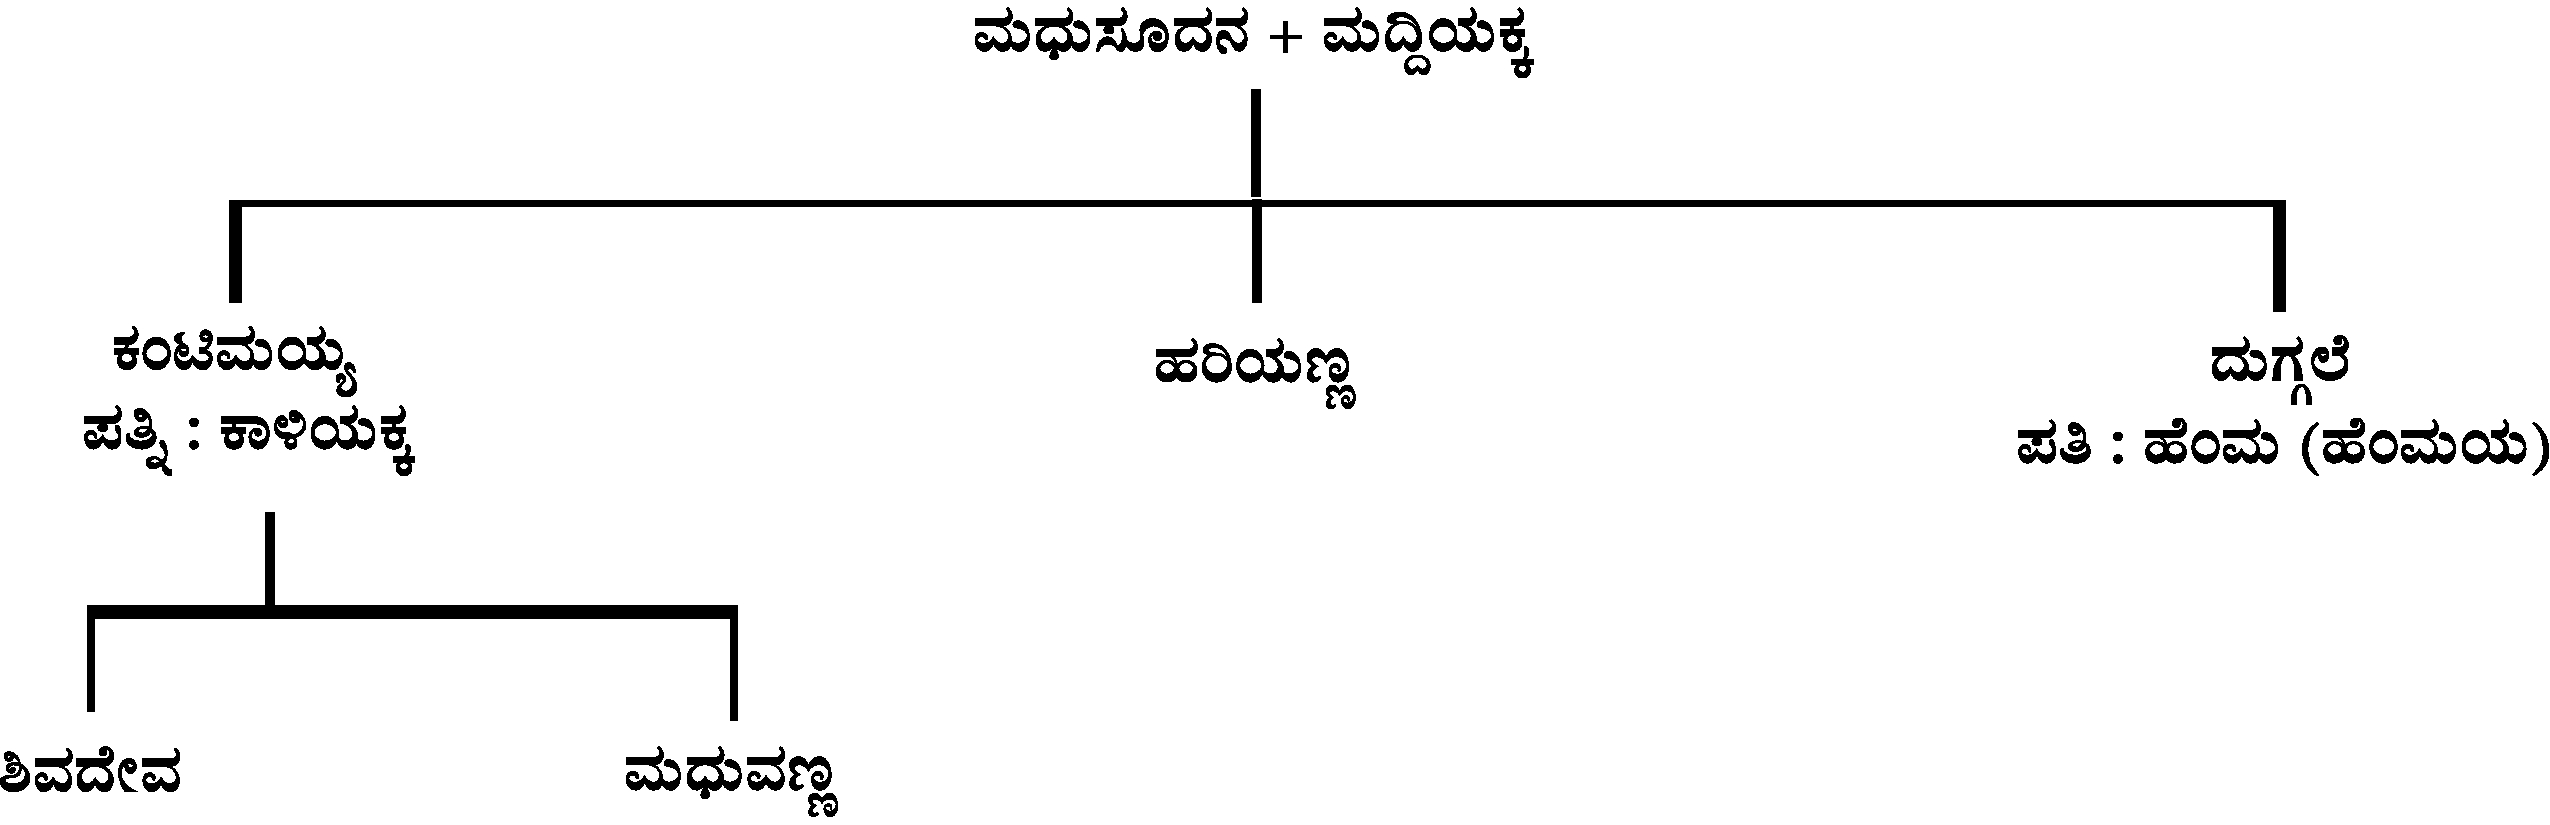
\includegraphics[scale=1.17]{images/chap3/chap3fig27.jpeg}
\end{figure}

\textbf{ಮಹಾಪ್ರಧಾನ\index{ಮಹಾಪ್ರಧಾನ} ಹಿರಿಯಹೆಗ್ಗಡೆ\index{ಹಿರಿಯಹೆಗ್ಗಡೆ} ಚಂದ್ರಮೌಳಿಯಣ್ಣ\index{ಚಂದ್ರಮೌಳಿಯಣ್ಣ} (1181):} ಇಮ್ಮಡಿ ಬಲ್ಲಾಳನ ಕಾಲದ ಮತ್ತೊಬ್ಬ ಪ್ರಖ್ಯಾತ ಮಹಾಪ್ರಧಾನಿ ಚಂದ್ರಮೌಳಿ ಅಥವಾ ಚಂದ್ರಮೌಳಿಯಣ್ಣ. ಶ‍್ರೀಮನ್​ ಮಹಾಪ್ರಧಾನಿ ಪೆರಿಯಮನೈ ಪೆರ್ಗ್ಗಡೆ\index{ಪೆರಿಯಮನೈ ಪೆರ್ಗ್ಗಡೆ} (ಹಿರಿಯ ಮನೆವೆರ್ಗ್ಗಡೆ\index{ಮನೆ ವೆಗ್ಗಡೆ (ವೆರ್ಗ್ಗಡೆ) (ಅರಮನೆಯ ಹೆಗ್ಗಡೆ)} ಅಥವಾ ಅರಮನೆಯ ಹಿರಿಯ ಹೆಗ್ಗಡೆ) ಚಂದ್ರಮೌಳಿಯಣ್ಣನ ತಮ್ಮನಾದ ಪಟ್ಟಯಾಂಗನಿಗೆ\index{ಪಟ್ಟಯಾಂಗ} ಬಿಟ್ಟಿದೇವನು\index{ಬಿಟ್ಟಿದೇವ} ಅಂದರೆ ವಿಷ್ಣುವರ್ಧನನು ಕೆಳಲೆನಾಡ\index{ಕೆಳಲೆ(ಕೆಳಲಿ)ನಾಡು} ತೆಂಕಭಾಗದಲ್ಲಿದ್ದ ಅನ್ನದಾನಪಳ್ಳಿಯನ್ನು\index{ಅನ್ನದಾನಪಳ್ಳಿ} ಅಗ್ರಹಾರವನ್ನಾಗಿ ಮಾಡಿ ದತ್ತಿಯಾಗಿ ನೀಡಿದ್ದನು.\endnote{ ಎಪಿಗ್ರಾಫಿಯಾ ಕರ್ನಾಟಿಕಾ, ಸಂಪುಟ 7, ಪೀಠಿಕೆ, ಪುಟ \engfoot{lix}} ತೆಂಪಾಗೈ ಮತ್ತು ಪಟ್ಟಯಙ್ಗನ್​ ಶಬ್ದಗಳಿಗೆ ತಜ್ಞರು ಬೇರೆ ಅರ್ಥವನ್ನು ನೀಡಿದ್ದಾರೆ. ಆದರೆ ಇದರ ಅರ್ಥ ತೆಂಕಣಭಾಗ ಮತ್ತು ಪಟ್ಟೆಯಾಂಗ ಎಂದಾಗುತ್ತದೆ. ಚಂದ್ರಮೌಳಿಯು ಆ ಅಗ್ರಹಾರದಲ್ಲಿದ್ದ ಕೈಲಾಸಸ್ಥಾನದಲ್ಲಿ\index{ಕೈಲಾಸಸ್ಥಾನ} (ಕೈಲಾಸನಾಥ ದೇವಾಲಯ) ಚಂದ್ರಮೌಳೀಶ್ವರ\index{ಚಂದ್ರಮೌಳೀಶ್ವರ} ದೇವರನ್ನು ಪ್ರತಿಷ್ಠೆಮಾಡಿ ವಿಣ್ಣಯಾಂಡರ\index{ವಿಣ್ಣಯಾಂಡ} ಮಗ ಮಹದೇವನನ್ನು ಅದರ ಸ್ಥಾನಪತಿಯಾಗಿ\index{ಸ್ಥಾನಪತಿ} ನೇಮಿಸುತ್ತಾನೆ.\endnote{ ಎಕ 7 ಮವ 34 ಅಂತರವಳ್ಳಿ 12ನೇ ಶ.} ಚಂದ್ರಮೌಳಿಯು ಶ್ರವಣಬೆಳಗೊಳದ ಅನೇಕ ಶಾಸನಗಳಲ್ಲಿ ಕೀರ್ತಿತನಾಗಿದ್ದಾನೆ. ಚಂದ್ರಮೌಳಿಯು ಶಂಭುದೇವ\index{ಶಂಭುದೇವ} ಮತ್ತು ಎಕ್ಕವ್ವೆಯರ\index{ಎಕ್ಕವ್ವೆ} ಮಗ. ಈತನ ಆರಾಧ್ಯದೈವ ಹರ(ಈಶ್ವರ). ಇವನ ಹೆಂಡತಿ ಆಚಿಕಬ್ಬೆ\index{ಆಚಿಕಬ್ಬೆ (ಆಚಿಯಕ್ಕ)}. ಇವಳ ವಂಶವೃಕ್ಷವನ್ನು ಶ್ರವಣಬೆಳಗೊಳದ ಶಾಸನಗಳು ನೀಡಿವೆ.\endnote{ ಎಪಿಗ್ರಾಫಿಯಾ ಕರ್ನಾಟಿಕಾ, ಸಂಪುಟ 2, ಪೀಠಿಕೆ, ಪುಟ lviii}

\begin{verse}
\textbf{ಪತಿಭಕ್ತಂ ವರಮಂತ್ರಶಕ್ತಿಯುತನಿಂದ್ರಗೆಂತು ಭಾಸ್ವದ್ಬೃಹ} \\\textbf{ಸ್ಪತಿ ಮಂತ್ರೀಶ್ವರನಾದಂತೆ ವಿಳಸದ್ಬಲ್ಲಾಳದೇವಾವನೀಪತಿಗೀ ವಿ} \\\textbf{ಶ್ರುತ ಚಂದ್ರಮೌಳಿ ವಿಭುದೇಶಂ ಮಂತ್ರಿಯಾದಂ ಸಮುಂನ} \\\textbf{ತತೇಜೋನಿಳಯಂ ವಿರೋಧಿಸಚಿವೋನ್ಮತ್ತೇಭ ಪಂಚಾನನ.\endnote{ ಎಕ 2 ಶ್ರಬೆ 44 ಶ್ರವಣಬೆಳಗೊಳ 1181}}
\end{verse}

\textbf{“ನುತಬಲ್ಲಾಳಭೂಪನ ದಕ್ಷಿಣಭುಜಾದಂಡನೆನಿಸಿದ್ದ ಚಂದ್ರಮೌಳಿಯು”} ತನ್ನ ಚಿತ್ತವಲ್ಲಭೆಯಾದ ಆಚಾಂಬಿಕೆ ಅಥವಾ ಆಚಿಯಕ್ಕನು ಶ್ರವಣಬೆಳಗೊಳದಲ್ಲಿ ಕಟ್ಟಿಸಿದ ಪಾರ್ಶ್ವಜಿನೇಶ್ವರ\index{ಪಾರ್ಶ್ವಜಿನೇಶ್ವರ} ಗೇಹದ ಪೂಜೆಗೆ ಬೊಮ್ಮೆಯನಹಳ್ಳಿಯನ್ನು ದತ್ತಿಯಾಗಿ ನೀಡಿದನು.\endnote{ ಎಕ 2 ಶ್ರಬೆ 571 ಬೊಮ್ಮನಹಳ್ಳಿ 1181} ಈತನು ಸ್ಮಾರ್ತಬ್ರಾಹ್ಮಣ\index{ಸ್ಮಾರ್ತ ಬ್ರಾಹ್ಮಣ} ಹಾಗೂ ಈಶ್ವರಭಕ್ತನಾದರೂ, ರುದ್ರಭಟ್ಟ\index{ರುದ್ರಭಟ್ಟ} ಕವಿಗೆ ಆಶ್ರಯ ನೀಡಿ ಅವನಿಂದ ವಿಷ್ಣುಪುರಾಣದ ಕೃಷ್ಣ ಕಥೆಯನ್ನು ‘ಜಗನ್ನಾಥವಿಜಯ’ವೆಂಬ\index{ಜಗನ್ನಾಥವಿಜಯ} ಚಂಪೂಕಾವ್ಯವನ್ನಾಗಿ ಬರೆಯಿಸಿದ್ದು ಸಾಹಿತ್ಯ ಚರಿತ್ರೆಯಿಂದ ತಿಳಿದುಬರುತ್ತದೆ.\endnote{ ಕನ್ನಡ ಸಾಹಿತ್ಯ ಚರಿತ್ರೆ, ಕನ್ನಡ ಅಧ್ಯಯನ ಸಂಸ್ಥೆ, ಸಂಪುಟ 4 ಭಾಗ 2, ಪುಟ 911, 919}


\section*{ದಂಡನಾಯಕರು\index{ದಂಡನಾಯಕರು (ದಂಡಾಧೀಶರು)} \enginline{-} ದಂಡಾಧೀಶರು\index{ದಂಡನಾಯಕರು (ದಂಡಾಧೀಶರು)}}

“ರಾಜನಿಂದ ಅಧಿಕಾರದ ಚಿಹ್ನೆಯಾಗಿ ದಂಡವನ್ನು ಪಡೆಯುತ್ತಿದ್ದುದರಿಂದ ಇವರನ್ನು ದಂಡನಾಯಕರು ಎಂದು ಕರೆಯಲಾಗು\-ತ್ತಿತ್ತು, ದಂಡನಾಯಕ ಶಬ್ದಕ್ಕೆ ಇದುವರೆಗೆ ಸೇನಾಪತಿ ಎಂಬ ಅರ್ಥವನ್ನು ಹೇಳುತ್ತಾ ಬರಲಾಗಿದೆ. ಆದರೆ ಇವರು ಚಕ್ರವರ್ತಿ ಅಥವಾ ಮಹಾ ಮಂಡಲೇಶ್ವರರಿಂದ ನೇಮಿಸಲ್ಪಟ್ಟ ಅಧಿಕಾರಿಗಳಾಗಿದ್ದು ಇವರಲ್ಲಿ ಕೆಲವರು ಸುಂಕಕ್ಕೆ, ಕೆಲವರು ಸೈನ್ಯಕ್ಕೆ, ಕೆಲವರು ವಿದೇಶಾಂಗಕ್ಕೆ ಹೀಗೆ ವಿವಿಧ ಇಲಾಖೆಗಳಿಗೆ ಸಂಬಂಧಪಟ್ಟವರಾಗಿದ್ದಾರೆ” ಎಂದು ವಿದ್ವಾಂಸರು ಹೇಳಿದ್ದಾರೆ.\endnote{ ನಾಗಯ್ಯ, ಡಾ. ಜೆ.ಎಂ., ಆರನೇ ವಿಕ್ರಮಾದಿತ್ಯನ ಶಾಸನಗಳು, ಒಂದು ಅಧ್ಯಯನ, ಪುಟ 320} ಆದರೆ ಇವರು ಮುಖ್ಯವಾಗಿ ಸೇನಾನಾಯಕರಾಗಿದ್ದರು. ಇವರ ಕೈಕೆಳಗೆ ಸೇನಾಪತಿ, ಸೇನಾಧಿಪತಿಗಳು, ಹಡವಳರು ಇರುತ್ತಿದ್ದರೆಂದು ಶಾಸನಗಳ ಆಧಾರದಿಂದ ಹೇಳಬಹುದು. ಇವರೂ ಕೂಡಾ ಮಂತ್ರಿಪರಿಷತ್ತಿನಲ್ಲಿ ಸ್ಥಾನಪಡೆದಿದ್ದರು ಎಂದೂ ತಿಳಿದುಬರುತ್ತದೆ.\endnote{ ಚಿದಾನಂದಮೂರ್ತಿ, ಡಾ॥ ಎಂ., ಕನ್ನಡ ಶಾಸನಗಳ ಸಾಂಸ್ಕೃತಿಕ ಅಧ್ಯಯನ, ಪುಟ 330}

ಹೊಯ್ಸಳರ ಶಾಸನಗಳಲ್ಲಿ ದಂಡನಾಯಕ ಬೊಪ್ಪದೇವ\index{ಬೊಪ್ಪದೇವ}\endnote{ ಎಕ 2 ಶ್ರಬೆ 506 ಶ್ರಬೆ 12ನೇ ಶ.} ಏಚದಂಡಾಧೀಶ\index{ಏಚಣ್ಣ ದಂಡನಾಯಕ}\endnote{ ಎಕ 2 ಶ್ರಬೆ 532 ಜಿನನಾಥಪುರ 12ನೇ ಶ.} ರೇಚಣ್ಣ ದಂಡನಾಯಕ\index{ರೇಚಣ್ಣ ದಂಡನಾಯಕ}\endnote{ ಎಕ 2 ಶ್ರಬೆ 528 ಜಿನನಾಥಪುರ 13ನೇ ಶ.} ಮಹಾಪ್ರಧಾನ ಅಂಕೆಯ ದಂಡನಾಯಕನ ಅಳಿಯ ಮಾಚಯ್ಯದಂಡನಾಯಕ\endnote{ ಎಕ 8 ಹಾಸನ 187ಅವ್ವೇರಹಳ್ಳಿ, 188 ಬನವಸೆ 1314} ಇವರನ್ನೆಲ್ಲಾ ದಂಡನಾಯಕರೆಂದು ಮಾತ್ರ ಕರೆಯಲಾಗಿದೆ. ಇವರಿಗೆ ಬೇರೆ ಯಾವುದೇ ಹುದ್ದೆಗಳಿಲ್ಲ. ಮಹಪ್ರಧಾನರೆಂದೂ ಇವರನ್ನು ಕರೆದಿಲ್ಲ. ಆದುದರಿಂದ ದಂಡನಾಯಕರ ಹುದ್ದೆ ಬೇರೆಯೇ ಆಗಿದ್ದು, ಅವರು ಮಹಾಪ್ರಧಾನ ದಂಡನಾಯಕರಿಗಿಂತ ಕೆಳಗಿನ ಹಂತದ ಅಧಿಕಾರಿಗಳೆಂದು ಹೇಳಬಹುದು. ಆರನೆಯ ವಿಕ್ರಮಾದಿತ್ಯನ ಶಾಸನಗಳಲ್ಲಿರುವಂತೆ ದಂಡನಾಯಕರಿಗೆ ಸುಂಕ ಹಾಗೂ ಇತರ ಇಲಾಖೆಗಳ ಅಧಿಕಾರಗಳನ್ನು ನೀಡಿದ್ದ ವಿಚಾರ ಹೊಯ್ಸಳರ ಶಾಸನಗಳಲ್ಲಿ ವಿವರವಾಗಿ ಬರುವುದಿಲ್ಲ.

ಜಿಲ್ಲೆಯ ಶಾಸನಗಳನ್ನು ಅವಲೋಕಿಸಿದಾಗ ಮಹಾಸಾಮಂತಾಧಿಪತಿ, ಮಹಾಪ್ರಚಂಡದಂಡನಾಯಕ ಎಂಬ ಹುದ್ದೆ\-ಗಳು ಕಂಡುಬರುವುದಿಲ್ಲ, ಕೇವಲ ಗಂಗರಾಜನನ್ನು ಮಾತ್ರ ಮಹಾಸಮಾಂತಾಧಿಪತಿ ಮತ್ತು ಮಹಾಪ್ರಚಂಡದಂಡನಾಯಕ ಎಂದು ಕರೆಯಲಾಗಿದೆ. ಉಳಿದಂತೆ ಎಲ್ಲರೂ ಮಹಾಪ್ರಧಾನ ದಂಡನಾಯಕರಾಗಿ ಅವರವರ ಶಕ್ತಿ ಸಾಮರ್ಥ್ಯಗಳಿಗನುಗುಣವಾಗಿ ವಿವಿಧ ಇಲಾಖೆಗಳನ್ನು ನಿರ್ವಹಿಸುತ್ತಿದ್ದುದನ್ನು ಈಗಾಗಲೇ ಪರಿಶೀಲಿಸಲಾಗಿದೆ. ಇನ್ನು ಕೆಲವರನ್ನು ಕೇವಲ ದಂಡನಾಯಕರೆಂದು ಕರೆಯಲಾಗಿದೆ. ಇವರಿಗೆ ಬೇರೆ ಯಾವ ಹುದ್ದೆಯನ್ನೂ ನೀಡಿರುವುದಿಲ್ಲ. ಇವರು ಮಹಾಪ್ರಧಾನ ದಂಡನಾಯಕರುಗಳ ಕೈಕೆಳಗೆ ಸೇನಾಬಲದ ಹಾಗೂ ವಿವಿಧ ಆಡಳಿತ ವಿಭಾಗದ ಮುಖ್ಯಸ್ಥರಾಗಿದ್ದರೆಂದು ಹೇಳಬಹುದು.

\textbf{ಅಳಿಸಂದ್ರ\index{ಅಳಿಸಂದ್ರ (ಅಳೀಸಂದ್ರ)} ಶಾಸನೋಕ್ತ ಡಾಕರಸ\index{ಡಾಕರಸ ದಂಡನಾಯಕ}, ಮರಿಯಾನೆ\index{ಮರಿಯಾನೆ (ದಂಡನಾಯಕ)} ಮತ್ತು ಇತರ ದಂಡನಾಯಕರು:} ಅಳಿಸಂದ್ರ ಶಾಸನವು ಅನೇಕ ಮಹಾಪ್ರಧಾನ ದಂಡನಾಯಕರು ಮತ್ತು ದಂಡನಾಯಕರ ಹೆಸರು ಮತ್ತು ವಿವರಗಳನ್ನು ನೀಡುತ್ತದೆ. ಈ ಶಾಸನದಲ್ಲಿ ಕೆಲವರನ್ನು ದಂಡನಾಯಕರೆಂದು, ಇನ್ನು ಕೆಲವರನ್ನು ಮಹಾಪ್ರಧಾನ ದಂಡನಾಯಕರೆಂದು ಬೇರೆಬೇರೆಯಾಗಿಯೇ ಹೇಳಿದ್ದು, ಇವೆರಡೂ ಬೇರೆ ಬೇರೆ ಹುದ್ದೆಗಳು, ಮಹಾಪ್ರಧಾನ ಕೇವಲ ಗೌರವಸೂಚಕವಾದ ಪದವಾಗಿರಲಿಲ್ಲ ಎಂಬುದು ಖಚಿತಪಡುತ್ತದೆ.

\textbf{ಡಾಕರಸ ದಂಡನಾಯಕ:} ಇವನು ಮರಿಯಾನೆ ವಂಶದ ಮೂಲ ಪುರುಷ. ಹಿರಿಯಮರಿಯಾನೆ\index{ಹಿರಿಯ ಮರಿಯಾನೆ ದಂಡನಾಯಕ} ದಂಡನಾಯಕನಿಗಿಂತ (ಕ್ರಿ.ಶ.1048) ಎರಡು ತಲೆಮಾರು ಹಿಂದಿನವನು. ಒಂದು ತಲೆಮಾರಿಗೆ 25 ವರ್ಷವೆಂದು ಇಟ್ಟುಕೊಂಡರೆ ಇವನು 10ನೇ ಶತಮಾನದ ಕೊನೆಗೆ (980\enginline{-}90) ಬರುತ್ತಾನೆ. ಕೌಂಡಿಲ್ಯ ಗೋತ್ರದ ಡಾಕರಸ ದಂಡನಾಯಕನ ಪತ್ನಿ ಏಚವ್ವೆ ದಣ್ನಾಯಕಿತಿ\index{ಏಚವ್ವೆ ದಣ್ನಾಯಕಿತಿ}. ಇವರಿಗೆ ನಾಕಣ ಮತ್ತು ಮರಿಯಾನೆ ದಂಡನಾಯಕ ಎಂಬ ಇಬ್ಬರು ಮಕ್ಕಳು. ಈ ಮರಿಯಾನೆ ದಂಡ ನಾಯಕನನ್ನು ಹಿರಿಯಮರಿಯಾನೆ ಅಥವಾ ಒಂದನೆಯ ಮರಿಯಾನೆ ದಂಡನಾಯಕನೆಂದು ಹೇಳಬಹುದು.

\textbf{ಹಿರಿಯಮರಿಯಾನೆ\index{ಹಿರಿಯ ಮರಿಯಾನೆ ದಂಡನಾಯಕ} ದಂಡನಾಯಕ: ಇವನನ್ನು ಒಂದನೆಯ ಮರಿಯಾನೆ\index{ಒಂದನೆಯ ಮರಿಯಾನೆ} ದಂಡನಾಯಕನೆಂದು ಹೇಳಲಾಗಿದೆ. }ಇವನು ವಿನಯಾದಿತ್ಯನ ಕಾಲದಲ್ಲಿ ದಂಡನಾಯಕನಾಗಿದ್ದನು. ದೇಕವ್ವೆ\index{ದೇಕಬ್ಬೆ, ದೇಕವ್ವೆ (ದಂಡನಾಯಕಿತ್ತಿ)} ಮತ್ತು ಚಾಮವ್ವೆ\index{ಚಾಮವ್ವೆ} ಇವನ ಪತ್ನಿಯರು.\break ದೇಕವ್ವೆ ದಂಡನಾಯಕತ್ತಿಗೆ ಮಾಚಣ ಮತ್ತು ಡಾಕರಸ(2) ಎಂಬ ಇಬ್ಬರು ಮಕ್ಕಳು. ಇವರಿಬ್ಬರೂ ದಂಡನಾಯಕರಾಗಿದ್ದರು. ಚಾಮವ್ವೆಗೆ ಪದ್ಮ, ಚಾಮಲೆ, ಬೋಪ್ಪಾದೇವಿ ಎಂಬ ಮೂವರು ಹೆಣ್ಣು ಮಕ್ಕಳು. ಇವರಿಗೆ ಒಂದನೆಯ ಬಲ್ಲಾಳನು\index{ಒಂದನೆಯ ಬಲ್ಲಾಳ} ವಿವಾಹ ಮಾಡಿದ ಸಂಗತಿಯನ್ನು ಹಿಂದೆಯೇ ವಿವರಿಸಲಾಗಿದೆ. ಮಾಚಣನ ಪತ್ನಿ ಹೆಮ್ಮವ್ವೆ ದಂಡನಾಯಕಿತಿ\index{ಹೆಮ್ಮವ್ವೆ (ದಂಡನಾಯಕಿತಿ)}. ಇವರ ಮಗಳು ಚಾಕಲೆ\index{ಚಾಕಲೆ}. ಚಾಕಲೆಯ ಗಂಡ ಕಾವರಾಜ. ಎರಡನೇ ಡಾಕರಸನ ಪತ್ನಿ ದುಗ್ಗವ್ವೆ ದಂಡನಾಯಕತ್ತಿ. ಇವರಿಗೆ ಎರಡನೆಯ ಮರಿಯಾನೆ\index{ಎರಡನೆಯ ಮರಿಯಾನೆ} ಮತ್ತು ಭರತ ದಂಡನಾಯಕ\index{ಭರತ (ಭರತಿಮಯ್ಯ) ದಂಡನಾಯಕ} ಎಂಬ ಇಬ್ಬರು ಮಕ್ಕಳು ಇವರಿಬ್ಬರೂ ಮಹಾ ಪ್ರಧಾನ ದಂಡನಾಯಕರಾಗಿದ್ದರು. ಇವರ ವಿವರಗಳನ್ನು ಈ ಹಿಂದೆಯೇ ಮಹಾ ಪ್ರಧಾನ ದಂಡನಾಯಕರ ವಿಭಾಗದಲ್ಲಿ ವಿವರಿಸಿದೆ. ಇವರ ವಂಶವೃಕ್ಷವನ್ನು ಹಿಂದೆಯೇ ನೀಡಿದೆ. ಹಿರಿಯ ಮರಿಯಾನೆಯ ಮಯ್ದುನ ಗಂಗರಾಜ ದಂಡಾಧೀಶ.

\textbf{ಕೊಮ್ಮರಾಜ ದಂಡನಾಥ\index{ಕೊಮ್ಮರಾಜ ದಂಡನಾಥ}:} ಒಂದನೆಯ ನರಸಿಂಹನ\index{ಒಂದನೆಯ ನರಸಿಂಹ} ಕಾಲದ ಸುಂಕಾತೊಂಡನೂರಿನ ಶಾಸನದಲ್ಲಿ \textbf{“ಮುನ್ನಸಂದ\general{\break } ದಂಡಾಧಿಪರೊಳತಿಶಯಂ ದಾನದೊಳು ಧರ್ಮದೊಳು ವಚನಶತಸಹಸ್ರ ಪ್ರತಾನಂಗಳೊಳು ಶೌರ್ಯಾಟೋಪದೊಳು\general{\break } ಸದ್ಗುಣದೊಳಧಿಕತೇಜಂ, ನೂರ್ಮಡಿ ಮಿಗಿಲೆನಿಪಂ ದಂಡನಾತಾಂಬರಾರ್ಕ್ಕಂ” }ಎಂಬುದಾಗಿ ಕೊಮ್ಮರಾಜ ದಂಡನಾಥನನ್ನು ಸ್ತುತಿಸಿದೆ.\endnote{ ಎಕ 6 ಪಾಂಪು 236 ಸುಂಕಾತೊಂಡನೂರು 12ನೇ ಶ.} ಈತನು ಕಮ್ಮೆಕುಲಕ್ಕೆ\index{ಕಮ್ಮೆಕುಲ} ಸೇರಿದವನು, ದ್ವಿಜ ವಂಶತಿಲಕನೂ\index{ದ್ವಿಜ ವಂಶತಿಲಕ}, ಕೌಶಿಕಗೋತ್ರ ಪವಿತ್ರನೂ ದಂಡಾಧೀಶದಾವಾನಲನೂ ಆಗಿದ್ದನೆಂದು ಶಾಸನದಲ್ಲಿ ಹೇಳಿದೆ. ಈತನು ಬಹುಶಃ ಸುಂಕಾತೊಂಡನೂರಿನಲ್ಲಿ\index{ಸುಂಕಾತೊಂಡನೂರು} ಬ್ರಹ್ಮಪುರಿಯನ್ನು\index{ಬ್ರಹ್ಮಪುರಿ} ಏರ್ಪಡಿಸಿದಂತೆ ಕಂಡುಬರುತ್ತದೆ. ಶಾಸನದಲ್ಲಿ ಒಂದುಕಡೆ “ಕೊಮ್ಮರಾಜಂ ಸ್ಥಿರನಾರಾಯಣಂ\index{ಸ್ಥಿರನಾರಾಯಣಂ}” ಎಂದು ಇರುವುದರಿಂದ ಇವನ ಹೆಸರು ಕೊಮ್ಮರಾಜನಿರಬಹುದು. ಇವನ ಪತ್ನಿಯ ಹೆಸರು ತ್ರುಟಿತವಾಗಿದೆ. ಈ ಶಾಸನವು ಸುಂಕಾತೊಂಡನೂರಿನ ಕೇಶವ ದೇವಾಲಯದ ಮುಂದೆ ಇದ್ದು, ಈ ದೇವಾಲಯವನ್ನೂ ಇವನೇ ನಿರ್ಮಿಸಿರುವ ಸಾಧ್ಯತೆ ಇದೆ. ಈ ಶಾಸನದಿಂದ ದಂಡಾಧೀಶರ ಪ್ರತ್ಯೇಕ ಹುದ್ದೆ ಇದ್ದಿತೆಂಬುದು ಸ್ಪಷ್ಟವಾಗುತ್ತದೆ.

\textbf{ಪಾರ್ಶ್ವದೇವ ದಂಡನಾಯಕ\index{ಪಾರ್ಶ್ವದೇವ ದಂಡನಾಯಕ}:} ಪಾರ್ಶ್ವದೇವನು ಒಂದನೆಯ ನರಸಿಂಹನ ಕಾಲದ ಪ್ರಸಿದ್ಧ ದಂಡನಾಯಕ. ಇವನ ತಂದೆ ನೇಮ ಮಂತ್ರೀಶ\index{ನೇಮ ಮಂತ್ರಿ (ಮಂತ್ರೀಶ-ದಂಡೇಶ)}. ತಾಯಿ ವಿಮಲ ಗಂಗಾನ್ವಯ\index{ವಿಮಲ ಗಂಗಾನ್ವಯ} ಖ್ಯಾತೆಯಾದ ಮುದ್ದರಸಿ\index{ಮುದ್ದರಸಿ}. ಪಾರ್ಶ್ವದೇವನು ಹನಸೋಗೆಯ ದಿವ್ಯ ಮುನಿಯ\index{ಹನಸೋಗೆಯ ದಿವ್ಯ ಮುನಿ} ಪಾದಾರ್ಚನೆಗೆ, ಅವನ ಜೊತೆಯಲ್ಲಿದ್ದ ಕಳಾಭ್ಯಸ್ತರಿಗೆ\index{ಕಳಾಭ್ಯಸ್ತರು} ಅಂದರೆ ಕಲೆಗಾರರಿಗೆ(ಇವರು ಶಿಲ್ಪಿಗಳೂ ಚಿತ್ರಕಾರರೂ ಆಗಿದ್ದಿರಬಹುದು) ಮತ್ತು ಮುನಿಗಳಿಗೆ, ಅವರ ಪರಂಪರೆಗೆ ದಾನವನ್ನು ನೀಡಿದನು.\endnote{ ಎಕ 7 ನಾಮಂ 26 1168 ಜನವರಿ31}

\begin{verse}
\textbf{ಧರೆತನ್ನಂ ಬಣ್ನಿಸಲ್ಬಿಂಡಿಗವಿಲೆಯೊಳಾ ನೇಮದಂಡೇಸದಿಕ್ಕುಂ} \\\textbf{ಜರಯ್ಯಂ ಪೆತ್ತ ತಾಯ್ಮುದ್ದರಸಿ ವಿಮಳಗಂಗಾನ್ವಯ ಖ್ಯಾತೆಯಾಗ} \\\textbf{ಲ್ದೊರೆವಿತ್ತೀ ಪಾರ್ಶ್ವದೇವ ಪ್ರಭು ಕಲಿಯುಗಭೀಮಾರ್ಹಗೇಹಾದಿ ಜೀರ್ಣೋ} \\\textbf{ದ್ಧರಣಂ ಗೆಯಾದವಗಂ ಸೋಭಿಸೆ ಸೋಧೆವೆಸನಂ ಗೆಯ್ಸಿದಂ}
\end{verse}

\newpage

ಕಲಿಯುಗಭೀಮನೆಂದು\index{ಕಲಿಯುಗಭೀಮ} ಪ್ರಸಿದ್ಧನಾಗಿದ್ದ ಪಾರ್ಶ್ವದೇವ ದಂಡನಾಯಕನು, ಅನೇಕ ಅರ್ಹಗೇಹಗಳನ್ನು\index{ಅರ್ಹಗೇಹ} ಅಂದರೆ ಬಸದಿ\-ಗಳನ್ನು ಜೀರ್ಣೋದ್ಧಾರ ಮಾಡಿಸಿ ಅವುಗಳಿಗೆ ಸುಣ್ಣಬಣ್ಣವನ್ನು ಮಾಡಿಸಿ, ಶೋಭಿಸುವಂತೆ ಮಾಡಿದನು. ದೇವಕ್ಷೇತ್ರವಾದ\index{ದೇವಕ್ಷೇತ್ರ} ಬಿಂಡಿಗನವಿಲೆಯೊಳಗೆ\index{ಬಿಂಡಿಗನವಿಲೆ} ಇಪ್ಪತ್ತನಾಲ್ಕು ಕಂಡುಗ ನೀರ್ನೆಲವನ್ನು\index{ಕಂಡುಗ ನೀರ್ನೆಲ} ಅಂದರೆ ಗದ್ದೆಯನ್ನು, ಐದು ಮತ್ತರು\index{ಮತ್ತರು} ಬೆದ್ದಲೆಯನ್ನು (ಹೊಲವನ್ನು) ಅರ್ಹಪೂಜೆಗೆ, ದಿವ್ಯವ್ರತ ಸಮಿತಿಗೆ\index{ದಿವ್ಯವ್ರತ ಸಮಿತಿ} ಮತ್ತು ವಿದ್ಯಾರ್ಥಿಗಳ ಅನ್ನದಾನಕ್ಕೆಂದು ಉತ್ಸಾಹದಿಂದ ನೀಡಿದನು. ವಿಷ್ಣುವರ್ಧನನ ಕಾಲದ ತಗಡೂರು.\endnote{ ಎಕ 10 ಚರಾಪ 52 ತಗಡೂರು 12ನೇ ಶ.} ಮತ್ತು ತೇರಣ್ಯ.\endnote{ ಎಕ 8 ಹೊನಪು 89 ತೇರಣ್ಯ 1122} ಶಾಸನಗಳಲ್ಲಿ, ನೇಮವೆರ್ಗಡೆ\index{ನೇಮವೆರ್ಗಡೆ} (ನೇಮಹೆರ್ಗಡೆ) ಎಂಬ ಅಧಿಕಾರಿಯ ಪ್ರಸ್ತಾಪವಿದೆ. ಈ ನೇಮ ಹೆಗ್ಗೆಡಯೇ, ಪಾರ್ಶ್ವದೇವ ದಂಡನಾಯಕನ ತಂದೆಯಾಗಿದ್ದು, ಮುಂದೆ ಉನ್ನತ ಹುದ್ದೆಗೆ ಬಡ್ತಿ ಪಡೆದು, ನೇಮದಂಡೇಶ\index{ನೇಮ ಮಂತ್ರಿ (ಮಂತ್ರೀಶ-ದಂಡೇಶ)} ಮಂತ್ರಿಯಾಗಿರಬಹುದು ಎಂದು ಊಹಿಸಬಹುದು.

\textbf{ನಾಗಯ್ಯ ದಂಡನಾಯಕ\index{ನಾಗಯ್ಯ ದಂಡನಾಯಕ}:} ನಾಗಯ್ಯ ದಂಡನಾಯಕನ ಭಾವ ಅರಿಯಪ್ಪನು, ಯಾದವನಾರಾಯಣ ಚತುರ್ವೇದಿ ಮಂಗಲವಾದ ತೊಂಡನೂರಿನ ಮಹಾಜನಗಳ ಜೊತೆ ಸೇರಿ, ಲಕ್ಷ್ಮೀನಾರಾಯಣ ಪೆರುಮಾಳಿಗೆ ಹರಹಿನ ಕಾಲುವೆಯ ಬಯಲಲ್ಲಿ ನೂರು ಕುಳಿ ಭೂಮಿಯನ್ನು ದತ್ತಿಯಾಗಿ ಬಿಡುತ್ತಾನೆ.\endnote{ ಎಇ 6 ಪಾಂಪು 69 ತೊಣ್ಣೂರು 1214} ಸಂತೆಶಿವರ ಶಾಸನೋಕ್ತ ವೀರನಾರಸಿಂಹದೇವರಸರ ಮಹಾಪ್ರಧಾನ ದಂಡನಾಯಕ ನಾಗದೇವ ದಂಣ್ನಾಯಕನೂ ಇವನೂ ಅಭಿನ್ನರೆಂದು ತೋರುತ್ತದೆ.\endnote{ ಎಕ 10 ಚರಾಪ 84 ಸಂತೆಶಿವರ 1236, ಚರಾಪ 86 ಸಂತೆಶಿವರ 1250} ದಂಡನಾಯಕನಾಗಿದ್ದ ಇವನು ಮುಂದೆ ಮಹಾಪ್ರಧಾನ ದಂಡನಾಯಕನ ಹುದ್ದೆಗೆ ಏರಿರಬಹುದು.

\textbf{ದಂಡನಾಯಕ ನಿಕ್ಕಿಯಣ್ಣ\index{ನಿಕ್ಕಿಯಣ್ಣ} ಅಥವಾ ನಿಕ್ಕಿಯರಸ\index{ನಿಕ್ಕಿಯರಸ}:} ಮೂರನೆಯ ನರಸಿಂಹನ ದಂಡನಾಯಕ ನಿಕ್ಕಯಣ್ಣನು ಪುಗಿರಿ ನಾಡಿನ\index{ಪುಗಿರಿನಾಡು(ಪೊಗರ್ನಾಡು)}, ಯಾದವಪುರದಲ್ಲಿ\index{ಯಾದವಪುರ} (ಇಂದಿನ ಪಾಂಡವಪುರ ತಾಲ್ಲೂಕು ಹೊಸಕೋಟೆ\index{ಹೊಸಕೋಟೆ}) ನಿಕ್ಕೀಶ್ವರ\index{ನಿಕ್ಕೀಶ್ವರ} (ನಿಷ್ಕಾಮೇಶ್ವರ\index{ನಿಷ್ಕಾಮೇಶ್ವರ ದೇವಾಲ}) ದೇವಾಲಯವನ್ನು ಜೀರ್ಣೋದ್ಧಾರ ಮಾಡಿ ದತ್ತಿಗಳನ್ನು ಬಿಟ್ಟಿರುವಂತೆ ತೋರುತ್ತದೆ.\endnote{ ಎಕ 6 ಪಾಂಪು 225 ಹೊಸಕೋಟೆ 1291-92} ಈ ನಿಕ್ಕೀಶ್ವರ ಅಥವಾ ನಿಷ್ಕಾಮೇಶ್ವರ ದೇವಾಲಯವು ವಿಷ್ಣುವರ್ಧನನ ಕಾಲದ ರಚನೆಯಾಗಿದೆ.\endnote{ ಎಕ 6 ಪಾಂಪು 229 ಹೊಸಕೋಟೆ 12 ನೇ ಶ.} ನಿಕ್ಕಿಯರಸನ ಮಗ ನಾಯಕದೇವ\index{ನಾಯಕದೇವಪಿಳ್ಳೆ}. ನಿಕ್ಕೀಶ್ವರ ದೇವಾಲಯದ ಸ್ಥಾನಪತಿ ಗೌತಮಗೋತ್ರದ ನಾಯಕದೇವಪಿಳ್ಳೆ\index{ನಾಯಕದೇವಪಿಳ್ಳೆ}, ಉಯ್ಯಕೊಂಡಪಿಳ್ಳೆ\index{ಉಯ್ಯಕೊಂಡಪಿಳ್ಳೆ}, ದಂಡನಾಯಕ ನಿಕ್ಕಿರಸ(ನಿಕ್ಕರಸ) ಮತ್ತು ಅವನ ಮಗ ನಾಯಕದೇವ ಈ ನಾಲ್ವರೂ ಸೇರಿ ರಾಜರಾಜಪುರ\-ವಾದ\index{ರಾಜರಾಜಪುರ} ತಲಕಾಡಿನ\index{ತಲಕಾಡು} ಸ್ಥಾನಪತಿ\index{ಸ್ಥಾನಪತಿ} ವೀರಭುಜಕ್ಕನ್ದೈಯರ್​ ಮಗ ಶಂಭುದೇವನಿಗೆ\index{ಶಂಭುದೇವ} ನಿಕ್ಕೀಶ್ವರ ದೇವಾಲಯದ ಅರ್ಚನಾವೃತ್ತಿಗೆ ಸೇರಿದ ಕನ್ನಯನಪಳ್ಳಿಯಲ್ಲಿ, ಒಂದು ವೃತ್ತಿಯನ್ನು ಮಾರಾಟಮಾಡುತ್ತಾರೆ. ವೃತ್ತಿಯ ಹಂಚಿಕೆಗಳಿಗೆ ಸಂಬಂಧಿಸಿದ ವಿಚಾರವನ್ನು ಅಲ್ಲೇ ಇರುವ ಇನ್ನೂ ಎರಡು ತ್ರುಟಿತ ತಮಿಳು ಶಾಸನಗಳು ಹೇಳುತ್ತವೆ.\endnote{ ಎಕ 6 ಪಾಂಪು 226 ಮತ್ತು 227 ಹೊಸಕೋಟೆ 1291-92}

\textbf{ಕಾಮೆಯ ದಂಡನಾಯಕ\index{ಕಾಮೆಯ ದಂಡನಾಯಕ}:} ಮುಮ್ಮಡಿ ಬಲ್ಲಾಳನು ಅಣ್ಣಾಮಲೆ ಪಟ್ಟಣದಿಂದ\index{ಅಣ್ಣಾಮಲೆ ಪಟ್ಟಣ} ಆಳುತ್ತಿದ್ದ ಕಾಲದಲ್ಲಿ, ಕನ್ನಂಬಾಡಿಯ\index{ಕನ್ನಂಬಾಡಿ}\break ಗೋಪಾಲಕೃಷ್ಣ ದೇವಾಲಯವನ್ನು\index{ಗೋಪಾಲಕೃಷ್ಣ ದೇವಾಲಯ (ಕನ್ನಂಬಾಡಿ)}, ಹದಿನೆಂಟು ಸಮಯದವರು\index{ಹದಿನೆಂಟು ಸಮಯ} ಸೇರಿ ಜೀರ್ಣೋದ್ಧಾರ ಮಾಡಿದಾಗ, ಈ ದೇವಾಲಯದ ಪೂಜಾಕಾರ್ಯಗಳಿಗೆ ಕಾಮೆಯ ದಣ್ಣಾಯಕನು ಹೊದಕೆ\index{ಹೊದಕೆ}, ಪೂರ್ಬ್ಬಾಯ\index{ಪೂರ್ಬ್ಬಾಯ (ಪೂರ್ವಾಯ)}, ಅಪೂರ್ಬ್ಬಾಯ\index{ಅಪೂರ್ಬ್ಬಾಯ (ಅಪೂರ್ವಾಯ)} ಮೊದಲಾದ ಮಾನ್ಯಗಳನ್ನು “ಸೇನಾಪತಿ ದತ್ತಿ” ಯಾಗಿ ಬಿಡುತ್ತಾನೆ. ಜೊತೆಗೆ ಮನೆಗಳನ್ನೂ ಕಟ್ಟಿಸಿಕೊಡುತ್ತಾನೆ.\endnote{ ಎಕ 6 ಪಾಂಪು 37 ಕನ್ನಂಬಾಡಿ 14ನೇ ಶ.} ದಂಡನಾಯಕ, ಸೇನಾಪತಿ ಇವೆರಡೂ ಸಮಾನ ಹುದ್ದೆಗಳೆಂದು ಇದರಿಂದ ತಿಳಿಯುತ್ತದೆ.

ಮುಮ್ಮಡಿ ಬಲ್ಲಾಳನ ಮಹಾಪ್ರದಾನ ಆದಿಸಿಂಗೆಯ ದಂಡನಾಯಕನು, ಮುಮ್ಮಡಿ ಬಲ್ಲಾಳನ ರಾಣಿವಾಸ\break ದೇಮಲಾದೇವಿಯ ಹೆಸರಿನಲ್ಲಿ, ಕಲ್ಲಹಳ್ಳಿಯನ್ನು ದೇವಲಾಪುರವೆಂಬ ಅಗ್ರಹಾರವನ್ನಾಗಿ ಮಾಡಿ ಮಹಾಜನಗಳಿಗೆ ಧಾರೆಯೆರೆಸಿ ಕೊಟ್ಟ ಶಿಲಾಶಾಸನವನ್ನು ಬರೆದುದಕ್ಕೆ, ಕಾಮೆಯ ದಂಡನಾಯಕರ ಸೇನ ಬೋವ ರಾಮಣ್ಣನು\index{ಸೇನಬೋವ ರಾಮಣ್ಣ} ಸಾಕ್ಷಿಯಾಗಿರುತ್ತಾನೆ. ಬಹುಶಃ ಕಾಮೆಯ ದಂಡನಾಯಕನು ವಡ್ಡವ್ಯವಹಾರಿ\index{ವಡ್ಡವ್ಯವಹಾರಿ}, ಉಭಯದೇಸಿ\index{ಉಭಯದೇಸಿ}, ನಾನಾದೇಸಿ\index{ನಾನಾದೇಸಿ (ದೇಶಿ)} ವ್ಯಾಪಾರಿಗಳಿಂದ ಇದಕ್ಕೆ ದತ್ತಿಯನ್ನು ಬಿಡಿಸಿರಬಹುದು. ಕ್ರಿ.ಶ.1214ರ ಅಮೃತಾಪುರ ಶಾಸನದಲ್ಲಿ ಕಾಮೆಯದಣ್ನಾಯಕರ ಮಗ ಮೇಳಯ್ಯನು, ಗುಜ್ಜರರೊಡನೆ ಹೋರಾಡಿ ಮಡಿದನೆಂದು ಹೇಳಿದೆ.\endnote{ ಎಕ 12 ತರಿಕೆರೆ 14 ಅಮೃತಾಪುರ 1214} ಕನ್ನಂಬಾಡಿ ಶಾಸನೋಕ್ತ ಕಾಮೆಯ ದಂಡನಾಯಕನು, ಅಮೃತಾಪುರ\index{ಅಮೃತಾಪುರ} ಶಾಸನೋಕ್ತ ಕಾಮೆಯ ದಂಡನಾಯಕನ ವಂಶದವನಿರಬಹುದು.

ಕಾಮೆಯ ದಂಡನಾಯಕನು ಮುಮ್ಮಡಿ ಬಲ್ಲಾಳನ ಕಾಲದಲ್ಲಿ ಮಹಾಪ್ರಧಾನ ದಂಡನಾಯಕನಾಗಿ ಅರೆನಕೆರೆಯ (ಅರಕೆರೆ)\index{ಅರಕೆರೆ} ಸ್ಥಳವನ್ನು ಆಳುತ್ತಿದ್ದನು. ಇವನ ತಂದೆ ಮಹಾಪ್ರಧಾನ ಪೊಂನಣ್ಣ. ಅನಾದಿ ಅಗ್ರಹಾರ ಬಲ್ಲಾಳನಪುರವಾದ ಕಿತ್ತನಕೆರೆಯನ್ನು ಕಾಮೆಯ ದಂಡನಾಯಕನು ‘ಸಬ್ಬಗೊಡುಗೆ\index{ಸಬ್ಬಗೊಡುಗೆ}’ಯಾಗಿ ನೀಡಿದ್ದನೆಂದು ತಿಳಿದುಬರುತ್ತದೆ.\endnote{ ಎಕ 10 ಅರಸೀಕೆರೆ 115 ಮಾಡಾಳು 1335} ಕಾಮೆಯದಂಡ\-ನಾಯಕನು ರಾಜ್ಯವಾಳುತ್ತಿದ್ದಾಗ, ತುರುಕರು\index{ತುರುಕರು} ಬಂದು ಕಲ್ಲಗುಂಡಿಯಹಳ್ಳಿಯನ್ನು\index{ಕಲ್ಲಗುಂಡಿಯಹಳ್ಳಿ} ಮುತ್ತಿದಾಗ, ಕಟಕತೋಟಿಕಾರ\index{ಕಟಕತೋಟಿಕಾರ} ಲಿಂಗಗವುಡನು\index{ಲಿಂಗಗವುಡ} ಕಾದಿ ಅವರ ಕುದುರೆಗಳನ್ನು ಹಿಡಿದುದಕ್ಕೆ, ಅವನಿಗೆ ಕಲ್ಲುಗುಂಡಿಯನ್ನು ಅದರ ಹಳ್ಳಿಗಳನ್ನೂ ನೆತ್ತರುಗೊಡಗೆಯಾಗಿ ನೀಡಿದನು.\endnote{ ಎಕ 10 ಅರಸೀಕೆರೆ 62 ಕಲ್ಗುಂಡಿ 1331} ಇದು ಮುಮ್ಮಡಿ ಬಲ್ಲಾಳನ ಕಾಲದಲ್ಲಿ ನಡೆದ ಮಹಮದೀಯರ ಆಕ್ರಮಣವಾಗಿರಬಹುದು\index{ಮಹಮದೀಯರ ಆಕ್ರಮಣ}. ಮಹಾಪ್ರಧಾನ ಪೆರಮಾಳೆದೇವ ದಂಡನಾಯಕನ\index{ಪೆರುಮಾಳೆ ದೇವ ದಂಡನಾಯಕ} ಮಗ ಅಲ್ಲಪ್ಪದಂಡನಾಯಕನು\index{ಅಲ್ಲಪ್ಪ ದಂಡನಾಯಕ}, ಇವನ ಮಯ್ದುನನಾಗಿದ್ದನೆಂದು ತಿಳಿದುಬರುತ್ತದೆ.\endnote{ ಎಕ 9 ಬೇಲೂರು 210 ಅಗ್ಗಡಲು 1328}


\section*{ಸೇನಾಪತಿಗಳು/ಸೇನಾಧಿಪತಿಗಳು/ಚಮೂಪರು}

ಸೇನಾಪತಿ ಅಥವಾ ಸೇನಾಧಿಪತಿಗಳು ಶ‍್ರೀಮನ್​ ಮಹಾಪ್ರಧಾನ ದಂಡನಾಯಕ, ಹಿರಿಯದಂಡನಾಯಕ, ದಂಡನಾಯಕ ಇವರ ಕೈಕೆಳಗೆ ಸೇನೆಯ ಮುಖ್ಯಾಧಿಕಾರಿಗಳಾಗಿ ಸೇನೆಯನ್ನು ಮುನ್ನಡೆಸುತ್ತಿದ್ದರೆಂದು ಹೇಳಬಹುದು. ಇವರಲ್ಲಿ ಕೆಲವರನ್ನು ಚಮೂಪರೆಂದೂ ಕರೆದಿದೆ. ಆದರೆ ಇವರನ್ನು ಎಲ್ಲಿಯೂ ಶ‍್ರೀಮನ್ಮಹಾಪ್ರಧಾನರೆಂದು ಕರೆದಿರುವುದಿಲ್ಲ.

\vskip 4pt

\textbf{ಸೇನಾಪತಿ ಕೇರಾಳನಾಯಕ\index{ಸೇನಾಪತಿ ಕೇರಾಳನಾಯಕ}:} ವಿಷ್ಣುವರ್ಧನನು\index{ವಿಷ್ಣುವರ್ಧನ (ದೇವರು) (ಹೊಯ್ಸಳರ ದೊರೆ)} ಬಂಕಾಪುರದ\index{ಬಂಕಾಪುರ} ಬೀಡಿನಿಂದ ರಾಜ್ಯವಾಳುತ್ತಿದ್ದಾಗ ಅವನ ಸೇನಾಪತಿ ಕೇರಾಳನಾಯಕನು ನಾಗರಘಟ್ಟದ\index{ನಾಗರಘಟ್ಟ} ಮಹಾದೇವರ ದೇವಾಲಯವನ್ನು\index{ಮಹಾದೇವರ ದೇವಾಲಯ} ಕಟ್ಟಿಸಿ, ಹತ್ತುಸಲಗೆ ಗದ್ದೆಯನ್ನು ಮೂವತ್ತುಕೊಳಗ ಕಾಡಕ್ಕಿಯನ್ನು\index{ಕಾಡಕ್ಕಿ} ದತ್ತಿಬಿಟ್ಟನು.\endnote{ ಎಕ 6 ಕೃಪೆ 60 ನಾಗರಘಟ್ಟ 12ನೇ ಶ.} ಈ ಶಾಸನದಲ್ಲಿ ಅವನನ್ನು \textbf{“ತುರಲೋಭತು ಟನಿಟುರ ಸೇನಾಪತಿ\index{ಸೇನಾಪತಿ}}” ಎಂದು ವರ್ಣಿಸಿದೆ. ಶಾಸನ ತ್ರುಟಿತವಾಗಿದೆ. ರಾಮನಾಥಪುರದ ಸಮೀಪ ಇರುವ ಕೇರಾಳಪುರವು\index{ಕೇರಾಳಪುರ} ಇವನ ಹೆಸರಿನಲ್ಲಿ ನಿರ್ಮಿತವಾಗಿರಬಹುದು.

\vskip 2pt

\textbf{ಸೇನಾಪತಿ ಚಟ್ಟೊಡೆಯ\index{ಸೇನಾಪತಿ ಚಟ್ಟೊಡೆಯ}:} ಮೂರನೆಯ ವೀನರಸಿಂಹನ ಸೇನಾಪತಿ ಚಟ್ಟೊಡೆಯನು, ತಳಕಾಡ\index{ತಲಕಾಡು} ಆನೆಬಸದಿಗೆ\index{ಆನೆಬಸದಿ}\break ಬಣ್ಣಿಗದೆರೆಹಳ್ಳಿಯನ್ನು ಹೊಯ್ಸಳದೇವರ ದತ್ತಿಯಾಗಿ ಬಿಡುತ್ತಾನೆ.\endnote{ ಎಕ 7 ಮವ 30 ಹುಸ್ಕೂರು 14 ನೇ ಶ.} ರಾಜನ ಪರವಾಗಿ ದತ್ತಿಗಳನ್ನು ಬಿಡುವ ಅಧಿಕಾರ ಸೇನಾಪತಿಗಳಿಗೆ ಇದ್ದಿತೆಂದು ಇದರಿಂದ ಊಹಿಸಬಹುದು. ಈ ಆನೆಬಸದಿಯು ಆದಿದೇವನ ಬಸದಿಯಾಗಿತ್ತೆಂದು ಅಲ್ಲೇ ಇರುವ ಕ್ರಿ.ಶ.1313ರ ಇನ್ನೊಂದು ಶಾಸನದಲ್ಲಿ ಹೇಳಿದೆ.\endnote{ ಎಕ 7 ಮವ 31 ಹುಸ್ಕೂರು 1313}

\vskip 2pt

\textbf{ಸೇನಾಪತಿ ಅಗತಿಯಪ್ಪ\index{ಸೇನಾಪತಿ ಅಗತಿಯಪ್ಪ}:} ಮೂರನೆಯ ಬಲ್ಲಾಳನ ಶ‍್ರೀಮನ್​ ಮಹಾಪ್ರಧಾನ ಗಡದ ಸಿಂಗೆಯ ದಂಡನಾಯಕನ\index{ಗಡದ (ಗಡ್ಡದ) ಸಿಂಗೆಯ ದಂಡನಾಯಕ} ಮಗ ಜಮರಂಣನು\index{ಜಮರಂಣ} ಚೆಂಗವಾಡಿಯ\index{ಚೆಂಗವಾಡಿ} ಶಿವಾಲಯಕ್ಕೆ ದತ್ತಿ ಬಿಟ್ಟಾಗ. ಸೇನಾಪತಿ ಅಗತಿಯಪ್ಪನ\index{ಸೇನಾಪತಿ ಅಗತಿಯಪ್ಪ} ಮಗನಿಗೆ (ಹೆಸರು ಸ್ಪಷ್ಟವಿಲ್ಲ), ಮತ್ತು ಅತುವಾಸುವಿನ ಮಗ ಮಾಯಣ್ಣನಿಗೆ, ಅರ್ಚನಾವೃತ್ತಿಯಾಗಿ ಬಂದಿದ್ದ ದತ್ತಿಗಳನ್ನು, ನಡೆಸಿಕೊಂಡು ಹೋಗುವ ಜವಾಬ್ದಾರಿಯನ್ನು ವಹಿಸಲಾಯಿತು. ಸೇನಾಪತಿ ಅಗತಿಯಪ್ಪನ ಬಗ್ಗೆ ಹೆಚ್ಚಿನ ವಿವರಗಳು ತಿಳಿದುಬರುವುದಿಲ್ಲ.\endnote{ ಎಕ 7 ಮವ 93 ಚೆಂಗವಾಡಿ 1305}

\vskip 2pt

\textbf{ಸೇನಾಪತಿ ವಡುಗಪಿಳ್ಳೈ\index{ಸೇನಾಪತಿ ವಡುಗಪಿಳ್ಳೈ}:} ತಲಕಾಡಿನಲ್ಲಿದ್ದ ಮೂಲಸ್ಥಾನ ಆನೆಬಸದಿಯ\index{ಆನೆಬಸದಿ} ಸ್ಥಾನಪತಿಗೆ, ಸೇನಾಪತಿ ವಡುಗಪಿಳ್ಳೆಯು ಕಿಳಲೆನಾಡ ಪುತ್ತೂರಿನಲ್ಲಿ, ಐದು ಜನ ಗಾವುಂಡರ ಸಮ್ಮುಖದಲ್ಲಿ ದತ್ತಿಗಳನ್ನು ಬಿಟ್ಟನೆಂದು, ಹುಸ್ಕೂರಿನಲ್ಲಿರುವ ತಮಿಳು ಶಾಸನದಿಂದ ತಿಳಿದುಬರುತ್ತದೆ.\endnote{ ಎಕ 7 ಮವ 29 ಹುಸ್ಕೂರು 12ನೇ ಶ.} ವಡುಗಪಿಳ್ಳೆಯು ಚೋಳರ ಸೇನಾಪತಿಯಾಗಿರಬಹುದು.


\section*{ಎಡಗೈಯ ಸೇನಾನಾಯಕರು/ಬಲಗೈಯ ಸೇನಾನಾಯಕರು}
\index{ಎಡಗೈ ಮೊತ್ತಕ}
\index{ಬಲಗೈ(ಯ) ಸೇನಾನಾಯಕ (ಸೇನಾಧಿಪತಿ)}

ಸೇನಾಧಿಪತಿಗಳಲ್ಲಿ ಎಡಗೈಯ ಸೇನಾನನಾಯಕರು, ಬಲಗೈಯ ಸೇನಾನಾಯಕರು ಎಂಬ ಎರಡು ರೀತಿಯ ನಾಯಕರಿದ್ದ\-ರೆಂದು ಜಿಲ್ಲೆಯ ಶಾಸನಗಳಿಂದ ತಿಳಿದುಬರುತ್ತದೆ. ಇದಕ್ಕೆ ಸಾಹಿತ್ಯದ ಆಧಾರಗಳೂ ಕೂಡಾ ಇದೆ. ಕುಮಾರರಾಮನ ಸಾಂಗತ್ಯದಲ್ಲಿ “ಬಲವಂಕದಲ್ಲಿ\index{ಬಲವಂಕ} ಶೂದ್ರಕುಲದ ಸಂಭೂತದ ಒಡ್ಡು, ಎಡವಂಕದಲ್ಲಿ\index{ಎಡವಂಕ} ಕೋಟಗಾರರ ಬಲುಫೌಜು” ಇದ್ದಿತೆಂಬ ವಿಷಯ ಬರುತ್ತದೆ.\endnote{ ರಾಮರಾವ್​. ಆರ್​.ಎಸ್​., ಸಮರಚಿತ್ರಗಳು, ಪುಟ 32} ಅಭಿಮನ್ಯುವು ಕೆಲಬಲಗಳಲ್ಲಿದ್ದ ಕಲಿಗಳನ್ನು ಸೀಳಿದನೆಂದು, ಸುಪ್ರತೀಕಗಜದ ಅಕ್ಕಪಕ್ಕದಲ್ಲಿ\break (ಬಹುಶಃ ಎಡಬಲಗಳಲ್ಲಿ) ಯೋಧರಿದ್ದರೆಂದು, ಸುಪ್ರತೀಕ ಗಜವು ಬಲಭಾಗದ ಸೇನೆಯ ಮೇಲೆ ನುಗ್ಗಿತೆಂದೂ ವಿವರಗಳು ದೊರೆಯುತ್ತವೆ.\endnote{ ಅದೇ- ಪುಟ25

ಕುಮಾರವ್ಯಾಸ ಭಾರತದ ದ್ರೋಣಪರ್ವ, ಅನುವಾದ ಎಲ್​.ಗುಂಡಪ್ಪ, ಪುಟ 717, 698, 699} ಊರಳಿವಿನಲ್ಲಿ ಕಿರಗತೂರ\index{ಕಿರಗತೂರ} ಹೆಗ್ಗಡೆ ಪರಮಗಾವುಂಡನ\index{ಪರಮಗಾವುಂಡ} ಮಗ ಮಾರಪ್ಪ, ಅವನ ಅಳಿಯ ಮಾದೆಯ ಎಡಗೈ\index{ಎಡಗಯ್ಯ ಸೇನಾನಾಯಕ}, ಬಲಗೈ\index{ಬಲಗೈ ಸೇನಾವೀರರು} ಆಗಿ ಕಾದಿ ಮಡಿದರೆಂದು ಕಿರಗಸೂರು\index{ಕಿರಗಸೂರು} ಶಾಸನದಲ್ಲಿ ಹೇಳಿದೆ.\endnote{ ಎಕ 7 ಮವ 101 ಕಿರಗಸೂರು 1285} ಇದರಿಂದ ಸೇನೆಯ ಚಲನೆ ಹಾಗೂ ಅವುಗಳ ನಾಯಕತ್ವ ವಹಿಸುತ್ತಿದ್ದ ವೀರರು, ಎಡಗೈ(ಎಡಭಾಗ) ಮತ್ತು ಬಲಗೈ(ಬಲಭಾಗ) ಎಂದು ಎರಡು ವಿಭಾಗಗಳಲ್ಲಿ ಹೋರಾಡುತ್ತಿದ್ದರೆಂದು, ಈ ಎರಡೂ ಕಡೆಯ ಸೇನೆಗಳಿಗೆ, ಸೇನಾಧಿಪತಿಗಳಿರುತ್ತಿದ್ದರೆಂದು ಹೇಳಬಹುದು. ಹೊಯ್ಸಳರ ಶಾಸನಗಳಲ್ಲಿ ಎಡಗೈ ಬಲಗೈ ಸೇನಾನಾಯಕರ ಕೆಲವು ವಿವರಗಳು ದೊರೆಯುತ್ತವೆ. ಶ‍್ರೀ ವೀರಬಲ್ಲಾಳ ರಾಯನ ಬಲವಂಕಪ್ಪ\index{ಬಲವಂಕಪ್ಪ} ನಾಯಕರಿಗೆ ಮುಖ್ಯಮಪ್ಪ ಗಂಡರಾಜ ಭೀಮರಾಯ\index{ಗಂಡರಾಜ ಭೀಮರಾಯ} ನಾಯಕನ ಪ್ರಸ್ತಾಪ ಚನ್ನಪಟ್ಟಣ\index{ಚನ್ನಪಟ್ಟಣ} ತಾಲ್ಲೂಕಿ ಮಳೂರು\index{ಮಳೂರು} ಶಾಸನದಲ್ಲಿದೆ.\endnote{ ಇ. ಸಿ. ಚನ್ನಪಟ್ಟಣ 150 ಮಳೂರು 1369} ಇಲ್ಲಿ ಬಲವಂಕ ಎಂದರೆ ಬಲಗೈಯ ಸೇನೆ ಎಂದು ಅದಕ್ಕೆ ಭೀಮರಾಯನು ಮುಖ್ಯನಾಗಿದ್ದನೆಂದು ಹೇಳಬಹುದು.

\textbf{ಬಲಗೈಯಸೇನಾಧಿಪತಿ\index{ಬಲಗೈ(ಯ) ಸೇನಾನಾಯಕ (ಸೇನಾಧಿಪತಿ)} ಸಾಮಂತ ಸೊಸಿಯಪ್ಪ\index{ಸಾಮಂತ ಸೊಸಿಯಪ್ಪ} (1191):} ವೀರಬಲ್ಲಾಳನ ಶ‍್ರೀಮತು ಬಲಗೈಯ ಸೇನಾಧಿಪತಿ ಸಾಮಂತ ಸೊಸಿಯಪ್ಪ ನಾಯಕನು, ರಾಜನ ಆದೇಶದಂತೆ ಬಡಗುಂದ ನಾಡ ಕೊತ್ತತ್ತಿಯ\index{ಬಡಗುಂದ ನಾಡ ಕೂತ್ತತ್ತಿ} ಮೇಲೆ ದಂಡೆತ್ತಿ ಹೋಗಿದ್ದು, ಇವನ ಜೊತೆ ಮುದಗಾವುಂಡನ ಮಗ ಸಾವಂತನ ಕಡೆಯ ಕೆಲವರು ಹೋರಾಡಿದಂತೆ, ಪೂರ್ಣವಾಗಿ ತ್ರುಟಿತವಾಗಿರುವ ವೀರಗಲ್ಲು ಶಾಸನದಿಂದ ಊಹಿಸಬಹುದು.\endnote{ ಎಕ 7 ಮಂ 78 ಮೊತ್ತಹಳ್ಳಿ 1191}

\vskip 2pt

\textbf{ಅಯ್ಯಾವೊಳೆ ವರ್ತಕಸಂಘದ\index{ಅಯ್ಯಾವೊಳೆ ವರ್ತಕಸಂಘ} ಬಲಗೈ ಸೇನಾವೀರರು\index{ಬಲಗೈ ಸೇನಾವೀರರು}:} ಅಯ್ಯಾವೊಳೆಯ ವರ್ತಕ ಸಂಘಕ್ಕೆ ಸೇರಿದ ಹದಿನೆಂಟು ಪಟ್ಟಣದ ಚೆಟ್ಟಿಯರನ್ನು\index{ಪಟ್ಟಣದ ಚೆಟ್ಟಿಯರು} ಅಂದರೆ ಸದಸ್ಯರನ್ನು ವರ್ಣಿಸುವ, ಧನಗೂರಿನ\index{ಧನಗೂರು (ಧನುಗೂರು - ಧನುರು)} ತ್ರುಟಿತ ತಮಿಳು ಶಾಸನದಲ್ಲಿ, “ಮುನ್ನೂರುಮ್ ಕೊಂಗಯರ್​ ಏಳುನೂರುಮ್ ಕೊಂಗುರಿಳಅಂಚಿಂಗರುಮ್ ವೀರರುಮ್ ಪೊರರ ಪಲಗೈಯಾನುಮ್ ಏಳುಬತ್ತೆಟ್ಟು\break ನಾಟ್ಟೋರ್ಗಳ್​” ಎಂದು ಹೇಳಿದೆ.\endnote{ ಎಕ 7 ಮವ 51 ಧನಗೂರು 13-14ನೇ ಶ.} ಅಂದರೆ ಕೊಂಗುನಾಡಿನಿಂದ ಬಂದಿದ್ದ ಮುನ್ನೂರು, ಏಳುನೂರು ಕೊಂಗರಿಳಂಚಿಂಗರು ಬಲಗೈಯ ಸೇನಾವೀರರಾಗಿದ್ದರು ಎಂದು ತಿಳಿಯಬಹುದು.

\textbf{ಹಾಲಿಮೊತ್ತದ\index{ಹಾಲಿಯಮೊತ್ತ} ಎಡಗಯ್ಯ ಸೇನಾನಾಯಕ\index{ಎಡಗಯ್ಯ ಸೇನಾನಾಯಕ} ಕಾಳೆಯ ನಾಯಕ\index{ಕಾಳೆಯ ನಾಯಕ} ಮತ್ತು ಮಲ್ಲೆನಾಯಕ\index{ಮಲ್ಲೆಯ ನಾಯಕ} (1218):} “ಸಂಭುರಾಯ ಕಾಡವರಾಯ ಕುಲಾನ್ವಯರಾದ” ಹಾಲಿಮೊತ್ತದ\index{ಹಾಲಿಯಮೊತ್ತ} ಎಡಗೆಯ್ಯ ಸೇನಾನಾಯಕ ಕಾಳೆಯನಾಯಕನ ತಮ್ಮ ಮಲ್ಲೆನಾಯಕ, ಅಪ್ಪೆಯನಾಯಕ\index{ಅಪ್ಪೆಯ ನಾಯಕ}, ಸಿವನೆನಾಯಕನ\index{ಸಿವನೆನಾಯಕ} ಮಗ ಕಲ್ಲೆಯನಾಯಕ\index{ಕಲ್ಲೆಯನಾಯಕ}, ಪೆಂಗೆನಾಯಕನ\index{ಪೆಂಗೆನಾಯಕ} ತಮ್ಮ ಸೋಮಯನಾಯಕನೊಳಗಾದ\index{ಸೋಮೆಯನಾಯಕ} ಸಮಸ್ತ ನಾಯಕರುಗಳು\index{ಸಮಸ್ತ ನಾಯಕರುಗಳು}, ಕಲುಕಣಿ ಯೆಪ್ಪತ್ತಕ್ಕೆ\index{ಕಲುಕಣಿ (ಕಲಿಕಣಿ-ಕಲ್ಕಣಿ-ಕಲ್ಕುಣಿ-ಕಲುಕರೆ) ನಾಡು} ಶಿರೋಮಣಿಯಂತಿದ್ದ ನಾನಲಕೆಱೆಯ (ಲಾಳನ ಕೆರೆ)\index{ನಾನಲಕೆರೆ (ಲಾಳನಕೆರೆ)} ಮಲ್ಲಿಕಾರ್ಜುನ ದೇವಾಲಯ, ಮಠಗಳಿಗೆ ಗದ್ದೆಬೆದ್ದಲುಗಳನ್ನು ದತ್ತಿಯಾಗಿ ಬಿಡುತ್ತಾರೆ. ಬಹುಶಃ ಈ ದೇವಾಲಯವನ್ನು ಇವರೇ ಕಟ್ಟಿಸಿರಬಹುದು.\endnote{ ಎಕ 7 ನಾಮಂ 62 ಲಾಳನಕೆರೆ 1218} “ಶಂಭುವರಾಯರು ಚೋಳರ ಸಾಮಂತರಾಗಿದ್ದು, ನಂತರ ಅವರ ಮೇಲೆ ತಿರುಗಿಬಿದ್ದರೆಂದೂ, ಎರಡನೆಯ ನರಸಿಂಹನು ಇವರನ್ನು ಅಡಗಿಸಿದನೆಂದೂ, ಪ್ರಸ್ತುತ ಶಾಸನದ ಸಂಭವರಾಯ ಕಾಡವರಾಯ ಕುಲಾನ್ವಯದ\index{ಸಂಭವರಾಯ ಕಾಡವರಾಯ ಕುಲಾನ್ವಯ} ಕಾಳೆಯನಾಯಕ, ಮಲ್ಲೆ\-ನಾಯಕರು ಆ ವಂಶಕ್ಕೆ ಸಂಬಂಧಪಟ್ಟವ\-ರಲ್ಲವೆಂದೂ” ಎಪಿಗ್ರಾಫಿಯಾ ಸಂಪಾದಕರು ಹೇಳಿರುವುದು ಸೂಕ್ತವಾಗಿದೆ.\endnote{ ಎಪಿಗ್ರಾಫಿಯಾ ಕರ್ನಾಟಿಕಾ, ಸಂಪುಟ 7, ಪೀಠಿಕೆ \engfoot{lix}} ಆದರೆ ಇವರನ್ನು ರಾಧೇಯ ಕುಲಧವಳ\index{ರಾಧೇಯ ಕುಲಧವಳ} ಹರ್ಮ್ಮ್ಯಮಾಣಿಕ್ಯ\index{ಹರ್ಮ್ಮ್ಯಮಾಣಿಕ್ಯ} ದೀಪಾಂಕುರನಂ” ಎಂದು ಹೇಳಿರುವುದರಿಂದ ಇವರು ರಾಧೇಯಕುಲ ಅಥವಾ ಹರ್ಮ್ಮ್ಯ ಕುಲಕ್ಕೆ ಸೇರಿದವ\-ರೆಂದು ಹೇಳಬಹುದು. (ಕರ್ಣನು ಸೂತಕುಲದ ರಾಧೇಯನ ಮಗನೆಂದು ಮಹಾಭಾರತ\-ದಲ್ಲಿ ಹೇಳಿದೆ.) ಸೂತ ನರಸಿಂಗಯ್ಯನ\index{ಸೂತ ನರಸಿಂಗಯ್ಯ} ಪ್ರಸ್ತಾವ ಕ್ರಿ.ಶ.1190ರ ಕಸಲಗೆರೆ\index{ಕಸಲಗೆರೆ} ಶಾಸನದಲ್ಲಿದ.\endnote{ ಎಕ 7 ನಾಮಂ 168 ಕಸಲಗೆರೆ 1190} ಇಂದಿನ ತಿಗಳ ಜನಾಂಗದಲ್ಲಿ “ಶಂಭು ಕುಲಕ್ಷತ್ರಿಯ\index{ಶಂಭು ಕುಲಕ್ಷತ್ರಿಯ}” ಎಂಬ ಒಂದು ಉಪಪಂಗಡವಿದ್ದು, ತಿಗಳರು\index{ತಿಗುಳರು} ವೀರರಾಗಿರುವುದರಿಂದ ಇವರು ಈ ಶಂಭುಕುಲ ಕ್ಷತ್ರಿಯ ವಂಶದವರಿರಬಹುದು.

ಈ ವಂಶದ ಮೂಲಪುರುಷ ಅತ್ಯಮನಾಯಕ\index{ಅತ್ಯಮನಾಯಕ}. ಇವನು \textbf{“ಕಱಿಗಟ್ಟಿದ ಕೋಟೆಗೆ ಲಗ್ಗೆ”} ಹಾಕಿ ವೈರಿಗಳನ್ನು ಎದುರಿಸಿ ಗೆಲ್ಲುತ್ತಿದ್ದನಂತೆ. ಇವನ ಮಗ ಅಪ್ಪೆಯ ನಾಯಕನ\index{ಅಪ್ಪೆಯ ನಾಯಕ} ಶೌರ್ಯದಿಂದ, ಬಲ್ಲಾಳನು ಯುದ್ಧಗಳನ್ನು ಗೆದ್ದನೆಂದು ತಿಳಿದುಬರುತ್ತದೆ. ನರಸಿಂಹನು ಮಲ್ಲೆನಾಯಕನಿಗೆ \textbf{“ಮಾನವರೊಳ್​ ಸೇವ್ಯನೆಂದು ನಾಯಕತನಮಂ ತಾನಿತ್ತು ರಕ್ಷಿಪಂ”} ಎಂದು ನಾಯಕತವನ್ನು ನೀಡಿದನು. ನಾಯಕತನ\index{ನಾಯಕತನ} ಎಂದರೆ ಸೇನಾನಾಯಕತನ ಎಂದು ಹೇಳಬಹುದು. ಇದನ್ನು ಬಿಟ್ಟರೆ ಇವರ ವರ್ಣನೆಯಲ್ಲಿ ಐತಿಹಾಸಿಕ ಅಂಶಗಳಾವುವೂ ಇಲ್ಲ. ಶಾಸನವು ಇವರ ವಂಶಾವಳಿಯನ್ನು ನೀಡಿದೆ. ಈ ಶಾಸನದಲ್ಲಿ ಬರುವ ಅನೇಕ ನಾಯಕರು ಮಲ್ಲೆನಾಯಕನ ಬಂಧುಗಳು, ಅನುಯಾಯಿಗಳೂ ಆಗಿರುವಂತೆ ತೋರುತ್ತದೆ. \textbf{“ಸ್ವಸ್ತಿ ಸಮ್ಮಸ್ತ ಗುಣಸಂಪನ್ನರಪ್ಪ ಕಟಕಕತ್ತಿ ಗಂಡರುಂ, ಗಂಡರ ಮೂಕುತಿಗಳುಂ, ಸರಣಾಗತ ವಜ್ರಪಂಜರರುಂ, ವೈರಿದಿಕ್ಕುಂಜರರುಂ, ಸಂಭುವರಾಯ ಕಾಡವರಾಯ ಕುಲಾನ್ವಯರುಂ, ಮಾರ್ಪ್ಪಾಡಿ ಗಂಡರುಂ, ಧನುರ್ವಿದ್ಯಾಪರಿಣತರುಂ, ಪರನಾರಿ ಸಹೋದರರು ಮುಖ್ಯವಪ್ಪ ಹಾಲಿಮೊತ್ತದ ಎಡಗೈಯ್ಯ ಸೇನಾನಾಯಕನಪ್ಪ ಕಾಳೆಯನಾಯಕನ ತಮ್ಮ ಮಲ್ಲನಾಯಕ”} ಎಂದು ಶಾಸನವು ವರ್ಣಿಸಿದೆ. ಶಾಸನದಿಂದ ಹೊರಡುವ ಇವರ ವಂಶಾವಳಿಯು ಈ ಕೆಳಗಿನಂತಿದೆ.

\begin{figure}[H]
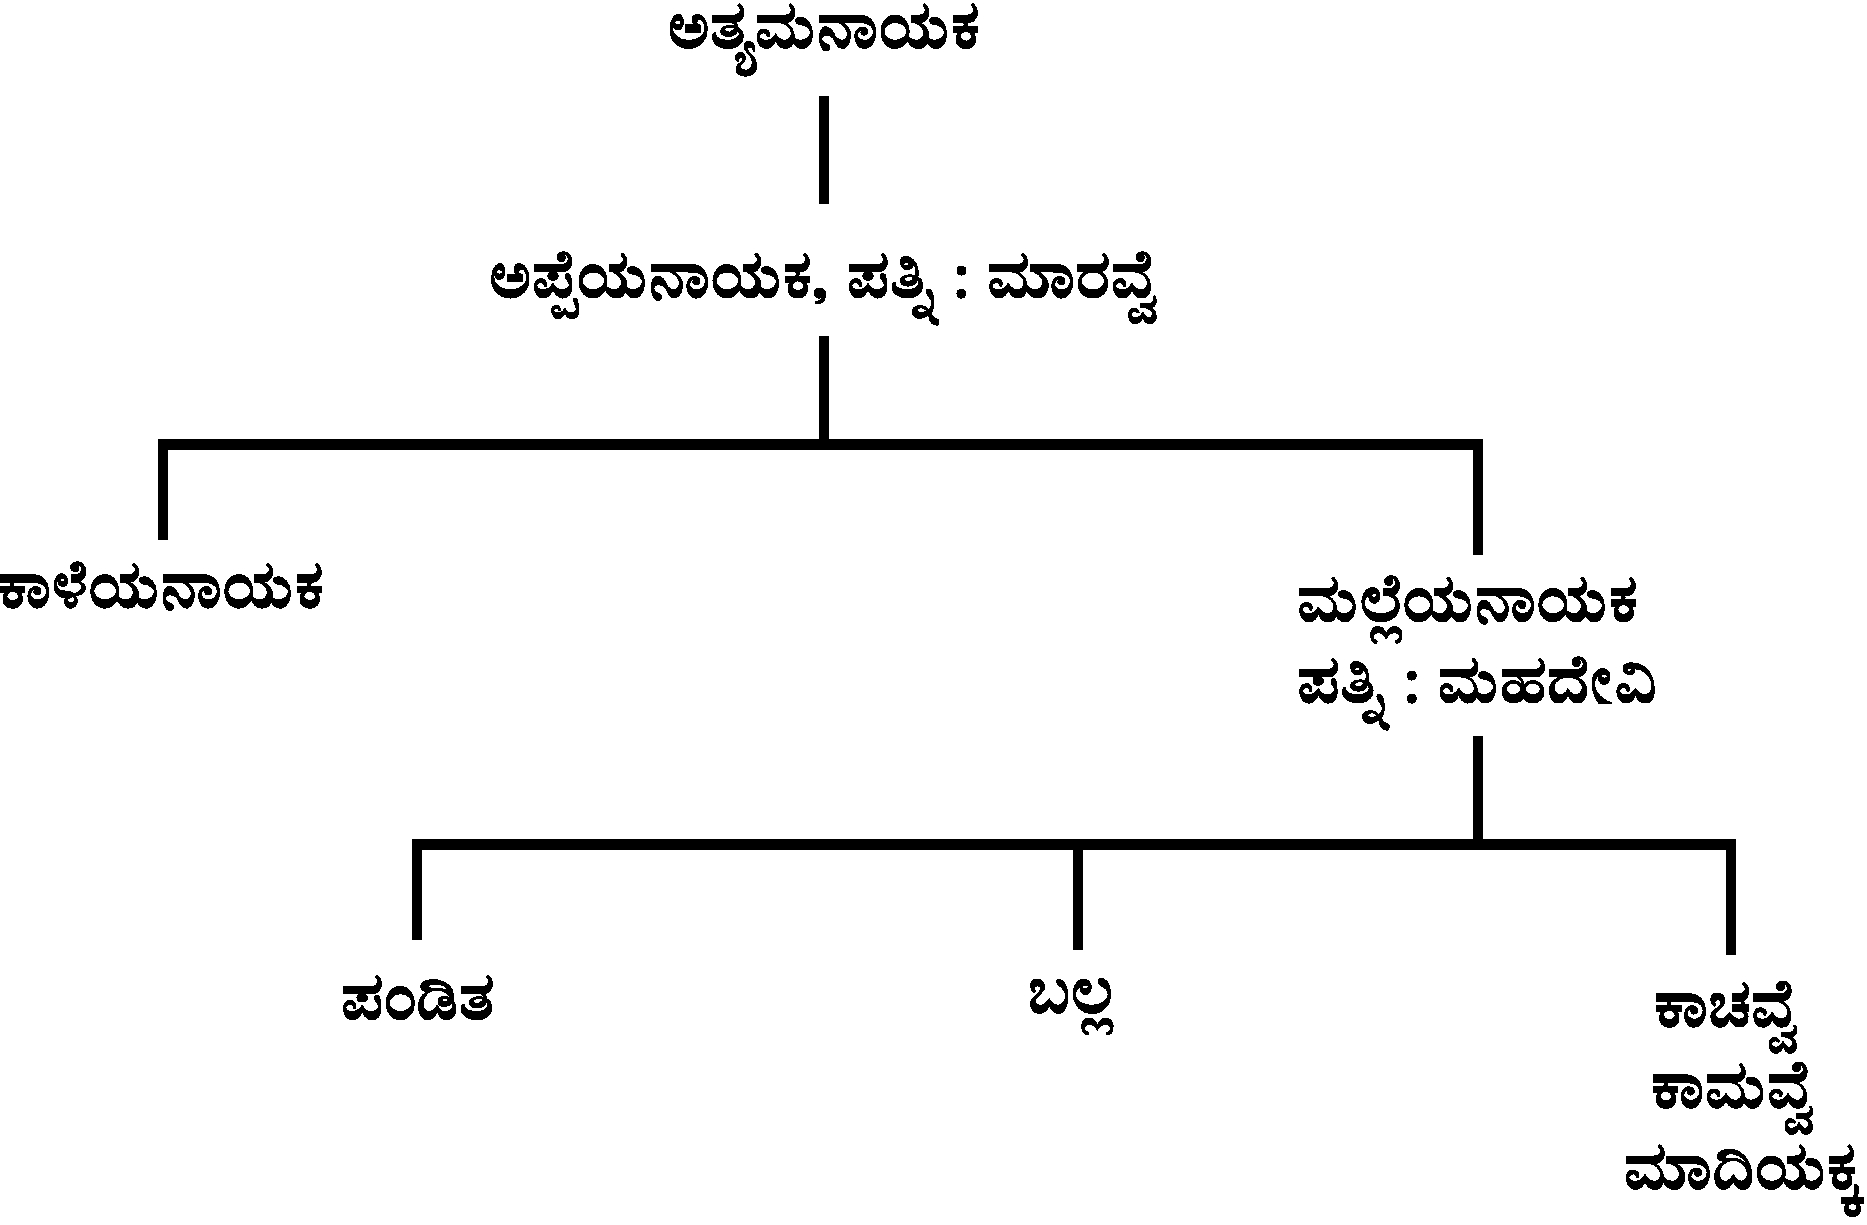
\includegraphics[scale=1.2]{images/chap3/chap3fig29.jpeg}
\end{figure}

\textbf{ಎಡಗೆಯ್ಯ (ಮೊತ್ತದ) ಸೇನಾನಾಯಕ\index{ಎಡಗೆಯ್ಯ (ಮೊತ್ತದ) ಸೇನಾನಾಯಕ} ಕಾಚೀದೇವ\index{ಕಾಚೀದೇವ} (13ನೇ ಶ.):} ಎರಡನೆಯ ನರಸಿಂಹನ ಕಾಲದಲ್ಲಿ ಅವನ ಮಹಾಸಾಮಂತ\-ನಾಗಿದ್ದ ಕಾಚೀದೇವನನ್ನು, ಎಡಗೈಯ ಮೊತ್ತದ ಸೇನಾನಾಯಕನಾಗಿದ್ದನೆಂದು\index{ಎಡಗೈಯ್ಯ (ಮೊತ್ತದ) ಸೇನಾನಾಯಕ} ಬೆಳ್ಳೂರು\index{ಬೆಳ್ಳೂರು} ಶಾಸನದಲ್ಲಿ ವರ್ಣಿಸ\-ಲಾಗಿದೆ.\endnote{ ಎಕ 7 ನಾಮಂ 81 ಬೆಳ್ಳೂರು 13 ನೇ ಶ.} ಇವನು ಮಹಾಸಾಮಂತನಾಗಿದ್ದರೂ, ಬಹಳ ವಿಶಿಷ್ಟವಾದ ಸೇನಾನಾಯಕ ಪದವಿಯನ್ನು ಹೊಂದಿದ್ದರಿಂದ, ಈ ವಂಶದವರ ವಿವರಗಳನ್ನು ಇಲ್ಲಿ ನೀಡಲಾಗಿದೆ. ಮೊತ್ತ ಎಂದರೆ ಒಟ್ಟು ಸೇನೆ ಅಥವಾ ಸೇನಾಬಲ ಎಂದು ಹೇಳಬಹುದು. ಇವನ ವಂಶದ ಮೂಲಪುರುಷ ನಂನಿಯಮೇರುವನ್ನು\index{ನಂನಿಯಮೇರು} \textbf{“ಎಡಗೈ ಮೊತ್ತಕ\index{ಎಡಗೈ ಮೊತ್ತಕ}”} ಎಂದು ಶಾಸನದಲ್ಲಿ ಹೇಳಿದೆ. ಮೇಲೆ ಉಲ್ಲೇಖಿಸಿದ ಎಡಗೈಯ ಸೇನಾನಾಯಕ ಕಾಳೆಯ ನಾಯಕನನ್ನು \textbf{“ಹಾಲಿಯಮೊತ್ತದ\index{ಹಾಲಿಯಮೊತ್ತ}}” ಎಂದು ಕರೆಯಲಾಗಿದೆ. ಆದುದರಿಂದ ಈ \textbf{ಮೊತ್ತಕ, ಮೊತ್ತದ ಎಂಬ ಶಬ್ದಗಳು ಸೇನಾಬಲಕ್ಕೆ ಸಂಬಂಧಿಸಿದೆ ಎಂದು ಹೇಳಬಹುದು}. “\textbf{ಬನವಸೆಕಾರರ ಮೊತ್ತದ ನಾಯಕರ\index{ಮೊತ್ತದ ನಾಯಕ}”} ಉಲ್ಲೇಖ ಚನ್ನರಾಯಪಟ್ಟಣ\index{ಚನ್ನರಾಯಪಟ್ಟಣ} ಶಾಸನದಲ್ಲಿದೆ.\endnote{ ಎಕ 10 ಚರಾಪ 12 ಚನ್ನರಾಯಪಟ್ಟಣ 1185} “ಮಗರನ ಮೇಲೆ ನಾರಸಿಂಗದೇವರು ನಡೆವಂದು \textbf{ಆಯಿದುಮೊತ್ತದ ಅಂಘರಕರಿಗೆ ಯೆಲೆಗನೂರ ಕೋಟೆಗೆ ಬೆಸಸಿದನೆಂದು”} ಹೇಳಿದೆ.\endnote{ ಎಕ 9 ಬೇಲೂರು 352 ಹಳೇಬೀಡು 1224} ಆಯಿದು ಮೊತ್ತ ಎಂದರೆ ಐದು ವಿಭಾಗ ಎಂದು ಹೇಳಬಹುದು. ಇಂದಿನ ಅರ್ಥದಲ್ಲಿ ಮೊತ್ತವನ್ನು ಸೇನೆಯ ಒಂದು ಡಿವಿಜನ್​ ಅಥವಾ ಬೆಟಾಲಿಯನ್​ಗೆ ಹೋಲಿಸಬಹುದೆಂದು ಕಾಣುತ್ತದೆ. ಸಿಂಗಯ್ಯ ಮತ್ತು ನಾಗಯ್ಯ ಇವರುಗಳನ್ನು \textbf{ಹಿರಿಯಭೇರುಂಡನ ಮೊತ್ತದ ಕೂಸುಗಳೆಂದು\index{ಮೊತ್ತದ ಕೂಸು}} ಕರೆದಿದೆ.\endnote{ ಎಕ 10 ಅರಸೀಕೆರೆ 117 ಮತ್ತು 118 ಹೊನ್ನಕಟ್ಟೆ 1209, 1214} ಎರಡನೆಯ ಬಲ್ಲಾಳನ ಮಗ ವೀರನರಸಿಂಹನು ದಿಗ್ವಿಜಯಾರ್ಥವಾಗಿ ಮತ್ತು ದುಷ್ಟನಿರ್ಮೂಲನೆಗಾಗಿ ಭೇರುಂಡವರ್ಗವನ್ನು\index{ಭೇರುಂಡವರ್ಗ} ಸ್ಥಾಪಿಸಿದನೆಂದು ತಿಳಿದುಬರುತ್ತದೆ.\endnote{ ಎಕ 10 ಚನ್ನರಾಯಪಟ್ಟಣ 63 ನವಿಲೆ 1218} ಇದೊಂದು ಸೇನಾತುಕಡಿ(ರೆಜಿಮೆಂಟ್​) ಆಗಿತ್ತೆಂದು ಎಪಿಗ್ರಾಫಿಯಾ ಸಂಪಾದಕರು ಅಭಿಪ್ರಾಯಪಟ್ಟಿದ್ದಾರೆ. ಕಾಚಿದೇವನ ವಂಶದ ಬಗ್ಗೆ ಈ ಹಿಂದೆ ವಿವರಿಸಲಾಗಿದೆ.

ಕಾಚಿಯ ನಾಯಕನ ವಂಶಸ್ಥರು ಹಟ್ಟಿಗಾಳೆಗಕ್ಕೆ\index{ಹಟ್ಟಿಗಾಳೆಗ} ಮಲೆವ ಸಾಮಂತರ ಗಂಡರಾಗಿದ್ದರೆಂದು ಹೇಳಿದೆ. ಹಟ್ಟಿಗಾಳೆಗ ಎಂಬುದು ಒಂದು ರೀತಿಯ ಯುದ್ಧವಾಗಿರಬಹುದು. ನಾಗಮಂಗಲ ತಾಲ್ಲೂಕಿನ ಸಮೀಪದಲ್ಲಿ “ಹಟ್ಟಿಯ ಲಕ್ಕಮ್ಮ\index{ಹಟ್ಟಿ ಲಕ್ಕಮ್ಮ}” ಎಂಬ ಪ್ರಸಿದ್ಧ ದೇವತೆಯ ದೇವಾಲಯವಿದ್ದು, ಈಕೆಯು ಹಟ್ಟಿಗಾಳೆಗ ಯುದ್ಧದ ದೇವತೆಯಾಗಿರಬಹುದು. ದೇವಾಲಯದ ಮುಂದೆ ವಿಶಾಲವಾದ ಜಾಗವಿದ್ದು, ಇದನ್ನು ಹಟ್ಟಿ ಎನ್ನುತ್ತಾರೆ.


\section*{ಹುಲಿಯ ಜಂಗುಳಿ\index{ಹುಲಿಯ ಜಂಗುಳಿ} ಪ್ರಮುಖ ಮುಖ್ಯರು}

ಮಹಾಸಾಮಂತ ಬರ್ಮಯ್ಯನನ್ನು\index{ಮಹಾಸಾಮಂತ ಬರ್ಮಯ್ಯ} “\textbf{ಹುಲಿಯಜಂಗುಳಿ ಪ್ರಮುಖಮುಖ್ಯ\index{ಹುಲಿಯಜಂಗುಳಿ ಪ್ರಮುಖಮುಖ್ಯ}”} ಎಂದು ಕಿಕ್ಕೇರಿ ಶಾಸನವು ಕರೆದಿದೆ.\endnote{ ಎಕ 6 ಕೃಪೇ 27 ಕಿಕ್ಕೇರಿ 1171} ಅದೇ ರೀತಿ ಮಹಾಸಾಮಂತ ನಾಗಯ್ಯನನ್ನು \textbf{ಹುಲಿಯಜಂಗುಳಿ ಮೊತ್ತದ ಸೇನಾನಾಯಕನೆಂದು} ಮರಡಿಪುರ\index{ಮರಡಿಪುರ} ಶಾಸನದಲ್ಲಿ ಹೇಳಿದೆ.\endnote{ ಎಕ 7 ಮಂ 13 ಮರಡಿಪುರ 1280} ಪಾಂಡ್ಯ ಮಹದೇವನ ಮೇಲೆ \textbf{“ಯಿಂದವರದ ಹುಲಿಯ ಜಂಗುಳಿ ಮಸಣಿತಂಮನ\index{ಮಸಣಿತಂಮ} ಮಗ ವೀರಮಸಣನು\index{ವೀರಮಸಣ} ಹೊಯಿದು ಕುಟ್ಟಾಡಿ ಸುರಲೋಕ ಪ್ರಾಪ್ತನಾದನೆಂದು”} ತಿಳಿದುಬರುತ್ತದೆ.\endnote{ ಎಕ 11 ಚಿಕ್ಕಮಗಳೂರು 25 ಇಂದಾವರ 1292} ಹುಲಿಯಜಂಗುಳಿ ಎಂಬುದು ಒಂದು ರೀತಿಯ ಸೇನಾಪಡೆ ಇರಬಹುದು. “ಸಂಥೆಶಾಸನ ಪೇಟೆ ಒಳಗಾದ ಸಮಸ್ತ ಹಳುವು ನಖರ ಪರಿವಾರ ಮುಮ್ಮುರಿ ದಂಡಂಗಳು ಸಕಲ ಸ್ವಾಮ್ಯವಂತರು ಅವರ ಕಾಲ್ಗಾಹಿನ ಬಿಲ್ಲಮೂಲೂ(ನೂರ್)ಪ್ಪಬ್ಬರು ಹೊಲಿಯಜಂಗುಲಿ(ಹುಲಿಯ ಜಂಗುಳಿ)\index{ಹೊಲಿಯಜಂಗುಲಿ(ಹುಲಿಯ ಜಂಗುಳಿ)} ಸಹಿತ ಶ‍್ರೀ ವಿರೂಪಾಕ್ಷದೇವರ ದಿವ್ಯ\-ಶ‍್ರೀಪಾದಪದ್ಮದ ಸನ್ನಿಧಿಯಲಿ ವಜ್ರಬೈಸಣಿಗೆಯನಿಕ್ಕಿ\index{ವಜ್ರಬೈಸಣಿಗೆ} ಕುಳ್ಳಿರ್ದ್ದು” ಎಂದು ಬೇಲೂರು ಶಾಸನದಲ್ಲಿ ಹೇಳಿದ್ದು, ಹುಲಿಯ ಜಂಗುಳಿಯವರು, ಕಾಲಾಳುಗಳ ಸೇನಾ ಪಡೆಯವರಾಗಿದ್ದು, ವ್ಯಾಪಾರಿವರ್ಗದವರಿಗೂ ರಕ್ಷಣೆ ನೀಡುತ್ತಿದ್ದರೆಂದು ಊಹಿಸ\-ಬಹುದು.\endnote{ ಎಕ 9 ಬೇಲೂರು 171 ಬೆಲೂರು 1382} ಹುಲಿಯ ಜಂಗುಳಿ ಎಂಬುದು ಸೇನೆಯಲ್ಲಿ ಬಳಸುವ ಒಂದು ಬಗೆಯ ವಾದ್ಯವಿಶೇಷವೋ ಅಥವಾ ಸೈನಿಕರು ಧರಿಸುತ್ತಿದ್ದ ಹುಲಿಯ ಮೊಗವಾಡವೋ ಆಗಿರಬಹುದು. “ನುಗ್ಗಿಹಳ್ಳಿಯ ರಾಯೊಡೆಯರ ಕುಮಾರ ಬಸವರಾಜಯ್ಯದೇವ ಮಹಾಅರಸನು ಶಾಂತಿಗ್ರಾಮದ\index{ಶಾಂತಿಗ್ರಾಮ} ನವರಂಗದ ಕಲ್ಲಬಾಗಿಲ ಕಟ್ಟಿಸಿ ಹುಲಿಮುಖವನಿಕ್ಕಿಸಿದನು” ಎಂದು ತಿಳಿದುಬರುತ್ತದೆ.\endnote{ ಎಕ 7 ಹಾಸನ 168 ಶಾಂತಿಗ್ರಾಮ 1573} ಕಂಠೀರವನರಸರಾಜ ಒಡೆಯರ ಕಾಲದಲ್ಲಿ ಹುಲಿಮುಖದ ಚಾವಡಿಯಲ್ಲಿ\index{ಹುಲಿಮುಖದ ಚಾವಡಿ} ವೀರೇಶ್ವರ\index{ವೀರೇಶ್ವರ}, ಭದ್ರಕಾಳಮ್ಮ\index{ಭದ್ರಕಾಳಮ್ಮ}, ಮಾಚಳೇಶ್ವರ\index{ಮಾಚಳೇಶ್ವರ} ದೇವರನ್ನು ಪ್ರತಿಷ್ಠಾಪಿಸಲಾಯಿತೆಂದು ಚನ್ನರಾಯಪಟ್ಟಣ\index{ಚನ್ನರಾಯಪಟ್ಟಣ} ಶಾಸನದಿಂದ ತಿಳಿದುಬರುತ್ತದೆ.\endnote{ ಎಕ 10 ಚರಾಪ 14 ಚನ್ನರಾಯಪಟ್ಟಣ 1648} ಹುಲಿಮುಖದ ಚಾವಡಿಯು ಯುದ್ಧಕ್ಕೆ ಸಂಬಂಧಿಸಿದ ಚಾವಡಿಯಾಗಿರ\-ಬಹುದು. ಇದರಿಂದ ಹುಲಿಯಜಂಗುಳಿ ಎಂದರೆ ಹುಲಿಮೊಗವಾಡವನ್ನು ಧರಿಸಿದ ಸೇನಾಪಡೆ ಎಂದು ಹೇಳಬಹುದು.


\section*{ಶ‍್ರೀಕರಣದ ಹೆಗ್ಗಡೆಗಳು\index{ಶ‍್ರೀಕರಣದ ಹೆಗ್ಗಡೆಗಳು}}

ಶ‍್ರೀಕರಣದ ಹೆಗ್ಗಡೆಗಳು ಅರಮನೆಯ ಲೆಕ್ಕಪತ್ರಗಳ ಇಲಾಖೆಯ ಅಧಿಕಾರಿಗಳು. ಇವರು ಶ‍್ರೀಮನ್​ಮಹಾಪ್ರಧಾನ ಸರ್ವಾಧಿಕಾರಿ ಶ‍್ರೀಕರಣದ ಹೆಗ್ಗಡೆಗಳ ಕೈಕೆಳಗೆ ಕೆಲಸ ಮಾಡುತ್ತಿದ್ದರೆಂದು ಹೇಳಬಹುದು. ಶ‍್ರೀಕರಣ ಸರ್ವಾಧಿಕಾರಿಗಳು ಲೆಕ್ಕಪತ್ರ ಇಲಾಖೆಯ ಮುಖ್ಯಸ್ಥರಾಗಿದ್ದರೆಂದೂ, ಇವರ ಕೆಳಗೆ ಶ‍್ರೀಕರಣದ ಹೆಗ್ಗಡೆಗಳು, ಗಣಕರು ಸೇವೆ ಸಲ್ಲಿಸುತ್ತಿದ್ದರೆಂದು ದೀಕ್ಷಿತ್​ ಅವರು ಹೇಳಿದ್ದಾರೆ.\endnote{ \engfoot{Dixith, Dr.G.S.,Local Self Government in Mediaeval Karnataka, pp. 16}} ಶ‍್ರೀಮನ್ಮಹಾಪ್ರಧಾನ ಸರ್ವಾಧಿಕಾರಿ ಮಹಾಪಸಾಯತ ಹಿರಿಯದಂಡನಾಯಕ ಮಾಚಿಮಯ್ಯನು ಕೊಂಗನಾಡನ್ನಾಳುತ್ತಿದ್ದಾಗ ಅವನ ಕೈಕೆಳಗೆ ನಾಲ್ಕು ಜನ ಶ‍್ರೀಕರಣಂಗಳು ಇದ್ದರೆಂದು ತಿಳಿಯುತ್ತದೆ.\endnote{ ಎಕ 8 ಅರಕಲಗೂಡು 134 ಸುಳಗೋಡುಸೋಮವಾರ 1189} ಶ‍್ರೀಕರಣದ ಬೂಚಿರಾಜನು ನಾರಸಿಂಹದೇವನ ಅರಮನೆಯಲ್ಲಿ ಸರ್ವಾಧ್ಯಕ್ಷನಾಗಿದ್ದನೆಂದು ತಿಳಿದುಬರುತ್ತದೆ.\endnote{ ಎಕ 8 ಹಾಸನ 128 ಕೋರವಂಗಲ 1173} ಹಾಸನ ತಾಲ್ಲೂಕು ಕೋರವಂಗಲದ ಶಾಸನಗಳಲ್ಲಿ ಈ ಶ‍್ರೀಕರಣದ ಮನೆತನದ ವಿವರಗಳಿವೆ. ನಾಕಯ್ಯನು ಕೊಂಗುದೇಶೈಕ ಶ‍್ರೀಕರಣಾಗ್ರಗಣ್ಯ\-ನಾಗಿದ್ದನು.\endnote{ ಎಕ 8 ಅರಕಲಗೂಡು 157 ಮಳಲಕೆರೆ 1284} ಹೀಗೆ ಅರಮನೆಯಲ್ಲಿ ಹಾಗೂ ರಾಜ್ಯದ ಕೇಂದ್ರಸ್ಥಳಗಳಲ್ಲಿ ಶ‍್ರೀಕರಣರು, ಶ‍್ರೀಕರಣಾಗ್ರಗಣ್ಯರು ಇದ್ದರೆಂದು ತಿಳಿಯುತ್ತದೆ. ಇವರನ್ನು ಶ‍್ರೀಕರಣದ ಹೆಗ್ಗಡೆಗಳೆಂದೂ ಕರೆದಿದೆ. ಶ‍್ರೀಕರಣದ ಸುಂಕವನ್ನು ದತ್ತಿಬಿಟ್ಟಿರುವ ವಿಚಾರ ಶಾಂತಿಗ್ರಾಮ ಶಾಸನದಲ್ಲಿದೆ.\endnote{ ಎಕ 8 ಹಾಸನ 160 ಶಾಂತಿಗ್ರಾಮ 1215} ಇದರಿಂದ ಶ‍್ರೀಕರಣದ ಸುಂಕವೆಂಬ ಒಂದು ವಿಶಿಷ್ಟವಾದ ಸುಂಕವಿತ್ತೆಂದು ಹೇಳಬಹುದು. ಇದನ್ನು ವಸೂಲು ಮಾಡುವ ಅಧಿಕಾರವೂ ಈ ಶ‍್ರೀಕರಣದ ಹೆಗ್ಗಡೆಗಳಿಗೆ ಇದ್ದಿತೆಂದು ಹೇಳಬಹುದು. ಇವರು ಹಣಕಾಸಿನ ಇಲಾಖೆಯ ಮುಖ್ಯಸ್ಥರಾಗಿ, ಶ‍್ರೀಮನ್ಮಹಾಪ್ರಧಾನ ದಂಡನಾಯಕರ, ಶ‍್ರೀಮನ್​ ಮಹಾಪ್ರಧಾನ ಹೆಗ್ಗಡೆಗಳ ಅಥವಾ ಶ‍್ರೀಮನ್​ಮಹಾಪ್ರಧಾನ ಶ‍್ರೀಕರಣದ ಹೆಗ್ಗಡೆಗಳ ಅಧೀನರಾಗಿ ಕಾರ್ಯವನಿರ್ವಹಿಸುತ್ತಿದ್ದರೆಂದು ಹೇಳಬಹುದು. ಶ‍್ರೀಕರಣದ ಹೆಗ್ಗಡೆಗಳೂ ಪಂಚಪ್ರಧಾನರಲ್ಲಿ ಒಬ್ಬರಾಗಿದ್ದರೆಂದು ತಿಳಿದುಬರುತ್ತದೆ.\endnote{ ಕೃಷ್ಣರಾವ್​ ಎಂ.ವಿ. ಪ್ರೊ॥, ಕರ್ನಾಟಕದ ಇತಿಹಾಸದರ್ಶನ, ಪುಟ 908} ಕರಣನೆಂದರೆ ಲೆಕ್ಕಬರೆಯುವ ಅಧಿಕಾರಿ ಎಂದು ಹೇಳಿರುವ ನಾಗಯ್ಯನವರು, ಮಹಾಪ್ರಧಾನ ಕರಣಕರು, ಶ‍್ರೀಕರಣರು, ಕರಣರು ಎಲ್ಲರನ್ನೂ ಕರಣಿಕರೆಂದೇ ಕರೆದಿದ್ದಾರೆ.\endnote{ ನಾಗಯ್ಯ,ಡಾ॥ ಜೆ.ಎಮ್., ಆರನೆಯ ವಿಕ್ರಮಾದಿತ್ಯನ ಶಾಸನಗಳು, ಪುಟ 358-59} ಆದರೆ ಹೊಯ್ಸಳ ಶಾಸನಗಳಲ್ಲಿ ಇವರೆಲ್ಲಾ ವಿವಿಧ ಹಂತದ ಅಧಿಕಾರಿಗಳಾಗಿದ್ದ\-ರೆಂಬುದು ಕಂಡು ಬರುತ್ತದೆ.

\textbf{ಶ‍್ರೀಕರಣದ ಹೆಗ್ಗಡೆ ಮಾದಿರಾಜ\index{ಮಾದಿರಾಜ} ಅಥವಾ ಶ‍್ರೀಕರಣದ ಮಾಧವ\index{ಶ‍್ರೀಕರಣದ ಮಾಧವ}:} ವಿಷ್ಣುವರ್ಧನ ಮತ್ತು ಒಂದನೇ ನಾರಸಿಂಹನ ಕಾಲದಲ್ಲಿದ್ದ ಶ‍್ರೀಕರಣದ ಹೆಗ್ಗಡೆ ಮಾದಿರಾಜನು ಭೋಗವತಿಯಲ್ಲಿ\index{ಭೋಗವತಿ(ದಿ)} (ಇಂದಿನ ಬೋಗಾದಿ\index{ಬೋಗಾದಿ}) ಶ‍್ರೀಕರಣ ಜಿನಾಲಯವನ್ನು\index{ಶ‍್ರೀಕರಣ ಜಿನಾಲಯ} ಕಟ್ಟಿಸಿ ಅಲ್ಲಿದ್ದ ದ್ರಮಿಳಸಂಘದ ಜೈನಯತಿಗಳಿಗೆ ದತ್ತಿಯನ್ನು ಬಿಟ್ಟನು.\endnote{ ಎಕ 7 ನಾಮಂ 183 ಬೋಗಾದಿ 1144} ಶಾಸನವು ಮಾದಿರಾಜನನ್ನು ಅವನ ವಂಶವನ್ನು ವಿವರವಾಗಿ ವರ್ಣಿಸಿದೆ, ಆದರೆ ಶಾಸನ ತ್ರುಟಿತವಾಗಿರುವುದರಿಂದ ವಿವರಗಳು ಸ್ಪಷ್ಟವಾಗಿ ತಿಳಿದುಬರುವುದಿಲ್ಲ. ಇವನ ವಂಶದವರು ಮನುಮಾರ್ಗಾಗ್ರಣಿಗಳು\index{ಮನುಮಾರ್ಗಾಗ್ರಣಿಗಳು} ಅಂದರೆ ಬ್ರಾಹ್ಮಣರಾಗಿದ್ದರೆಂದು, ಪಿತಾಮಹನ ಹೆಸರು ನಾರಾಯಣನೆಂದೂ\index{ನಾರಾಯಣ} ಅವನು ಗಂಗರಕಾಲದಲ್ಲಿ ಮಹಾಪ್ರಧಾನನಾಗಿದ್ದನೆಂದು, ಇವನ ತಾಯಿಯ ಹೆಸರು ಉಮೆಯಕ್ಕನೆಂದೂ\index{ಉಮೆಯಕ್ಕ}, ತಂದೆಯ ಹೆಸರು\break ವೋಣಮಯ್ಯನೆಂದು, ಇವನ ಗುರುಗಳು ಅಜಿತಸೇನರೆಂದು\index{ಅಜಿತಸೇನ}, ವಿಷ್ಣುವರ್ಧನನೇ\index{ವಿಷ್ಣುವರ್ಧನ (ದೇವರು) (ಹೊಯ್ಸಳರ ದೊರೆ)} ಅವನನ್ನು ಪೊರೆದನೆಂದೂ, ಶಾಸನದಲ್ಲಿ ಉಳಿದಿರುವ ಮಾಹಿತಿಯಿಂದ ಊಹಿಸಬಹುದು. ಶಾಸನದಲ್ಲಿ ಇವನ ಗುರುಪರಂಪರೆಯನ್ನು ನೀಡಿದ್ದು, ಮಾದಿರಾಜನ ಗುರುಗಳು ಶ‍್ರೀಪಾಳತ್ರೈವಿದ್ಯದೇವರೆಂದು\index{ಶ‍್ರೀಪಾಳತ್ರೈವಿದ್ಯದೇವರು}, ಇವರು ದ್ರಮಿಳ ಸಂಘಕ್ಕೆ\index{ದ್ರಮಿಳ ಸಂಘ} ಸೇರಿದ್ದರೆಂದು ಹೇಳಿದೆ. ಅಲ್ಲೇ ಇರುವ ಇನ್ನೊಂದು ಶಾಸನದಲ್ಲಿ ವಿಭು ಮಾಚಿರಾಜನು ಇಮ್ಮಡಿ ಬಲ್ಲಾಳನ ಮಹಾಪ್ರಧಾನ ಸರ್ವಾಧಿಕಾರಿ ಹೆಗ್ಗಡೆ ಬಲ್ಲಯ್ಯನ ಕೈಯಲ್ಲಿ ಈ ಶ‍್ರೀಕರಣ ಜಿನಾಲಯಕ್ಕೆ ಬೋಗವದಿಯ ಸಮಸ್ತ ಸುಂಕವನ್ನು ಬಿಡಿಸಿದನೆಂದು ಹೇಳಿದೆ.\endnote{ ಎಕ 7 ನಾಮಂ 184 ಬೋಗಾದಿ 1173} ಈ ದತ್ತಿಯನ್ನು ಪಡೆದವನು ಅಕಳಂಕನ\index{ಅಕಳಂಕದೇವರು} ಶಿಷ್ಯ ಪದ್ಮಪ್ರಭನೆಂದು\index{ಪದ್ಮಪ್ರಭ} ಹೇಳಿದೆ. ಮಾದಿರಾಜನ ವಂಶಾವಳಿ.

\begin{figure}[H]
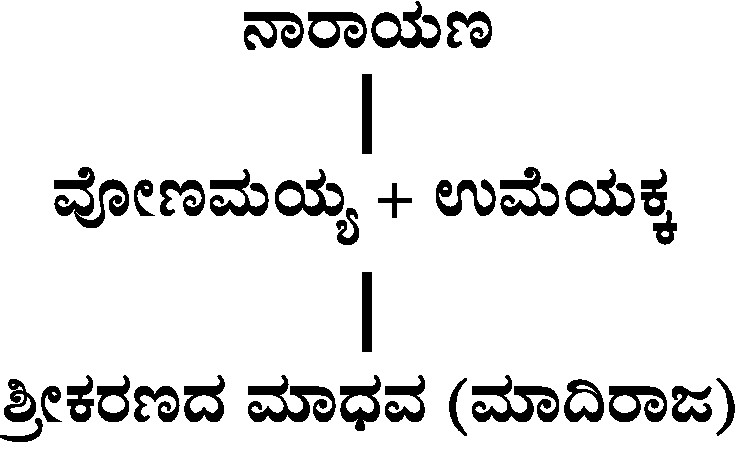
\includegraphics[scale=1.3]{images/chap3/chap3fig30.jpeg}
\end{figure}

\textbf{ಶ‍್ರೀಕರಣದ ಹೆಗ್ಗಡೆ ಕಲಿಯಣ್ಣ\index{ಕಲಿಯಣ್ಣ}:} ಶ‍್ರೀಕರಣದ ಹೆಗ್ಗಡೆ ಕಲಿಯಣ್ಣನು ಇಮ್ಮಡಿ ಬಲ್ಲಾಳನ ಕಾಲದಲ್ಲಿದ್ದನು. ಈತನು ತನ್ನ ಮೇಲಿನ ಅಧಿಕಾರಿಯಾಗಿದ್ದ, ಶ‍್ರೀಮನ್​ ಮಹಾಪ್ರಧಾನ ಸರ್ವಾಧಿಕಾರಿ ಮಹಾಪಸಾಯ್ತ ಶ‍್ರೀಕರಣದ ಹೆಗ್ಗಡೆ\index{ಶ‍್ರೀಕರಣದ ಹೆಗ್ಗಡೆ} ಎರೆಯಣ್ಣನ ಕೈಲಿ ಒಂಬತ್ತು ವೃತ್ತಿಯನ್ನು ಕ್ರಯದಾನವಾಗಿ ಕೊಂಡು, ಅದನ್ನು ಕಾಂಚೀಪುರದ ಅಲ್ಲಾಳಪೆರುಮಾಳೆ\index{ಕಾಂಚೀಪುರದ ಅಲ್ಲಾಳಪೆರುಮಾಳೆ} ದೇವರಿಗೆ.\endnote{ ಎಕ 6 ಪಾಂಪು 64 ತೊಣ್ಣೂರು 1175} ಕ್ರಯದ ಹೊನ್ನನ್ನು ಕೊಟ್ಟು ಐವತ್ತು ಕೊಳಗ ಗದ್ದೆಯನ್ನು, ಸಾವಿರಕೊಳಗ ಬೆದ್ದಲೆಯನ್ನು ಖರೀದಿಸಿ ಕ್ಯಾತನಹಳ್ಳಿಯ\index{ಕ್ಯಾತನಹಳ್ಳಿ} ಕೊಡೆಹಾಳ ಬಸದಿಗೆ\index{ಕೊಡೆಹಾಳ ಬಸದಿ} ದತ್ತಿಯಾಗಿ ಬಿಡುತ್ತಾನೆ.\endnote{ ಎಕ 6 ಪಾಂಪು 15 ಕ್ಯಾತನಹಳ್ಳಿ 1175} ಆದುದರಿಂದ ಶ‍್ರೀಕರಣದ ಹೆಗ್ಗಡೆಗಳು ಶ‍್ರೀಮನ್​ಮಹಾಪ್ರಧಾನ ಶ‍್ರೀಕರಣದ ಹೆಗ್ಗಡೆಗಳ ಕೈಕೆಳಗೆ ಕೆಲಸ ಮಾಡುತ್ತಿದ್ದರು ಎಂಬುದು ಖಚಿತವಾಗುತ್ತದೆ.


\section*{ಬಹಿತ್ರದ ಹೆಗ್ಗಡೆಗಳು\index{ಬಹಿತ್ರದ ಹೆಗ್ಗಡೆಗಳು}}

ಬಹಿತ್ರದ ಹೆಗ್ಗಡೆಗಳು ವಿವಿಧ ಇಲಾಖೆಗಳ ವ್ಯವಹಾರವನ್ನು ನೋಡಿಕೊಳ್ಳುತ್ತಿದ್ದರೆಂದು ಹೇಳಬಹುದು. ಬಹಿತ್ರ ಎಂಬುದು ಭೈತ್ರ\index{ಭೈತ್ರ}, ಬಾಹತ್ತರ, ಎಂಬುದರ ರೂಪ ಎಂದು ಕಿಟ್ಟೆಲ್​ರವರು ಹೇಳುತ್ತಾರೆ.\endnote{ ಕಿಟ್ಟೆಲ್​, ಕನ್ನಡ-ಇಂಗ್ಲಿಷ್​ ಡಿಕ್ಷ್​ನರಿ, ಪುಟ 1178, 1109} ಭೈತ್ರ ಎಂಬುದಕ್ಕೆ ಹಡಗು, ಕೂಟ ಎಂದೂ ಅರ್ಥವಿದೆ. “ಜಳಧಿಯೊಳ್​ ಬೈತ್ರಂ ಪರಿವಂತೆ” “ಬೀೞ್ಗುಂಡಿಕ್ಕಿದ ಬಹಿತ್ರದಂತೆ” ಎಂದು ಪಂಪನ ಆದಿಪುರಾಣದಲ್ಲಿ ಹೇಳಿದ್ದು ಬಹಿತ್ರ ಎಂದರೆ ಹಡಗು ಎಂಬ ಅರ್ಥವಿದೆ.\endnote{ ಆದಿಪುರಾಣ, 12ನೇ ಆಶ್ವಾಸ, ಪದ್ಯ 83 ಮತ್ತು 85ರ ನಂತರದ ವಚನ ಖಂಡಗಳು.} ಹೊಯ್ಸಳರ ಶಾಸನಗಳಲ್ಲಿ ಬಾಹತ್ತರ ನಿಯೋಗಾಧಿಪತಿ ಎಂಬ ಹುದ್ದೆಯ ಉಲ್ಲೇಖ ಅನೇಕ ಕಡೆ ಬರುತ್ತದೆ. ಬಾಹತ್ತರ ಎಂದರೆ ಎಪ್ಪತ್ತೆರಡು. ಎಪ್ಪತ್ತೆರಡು ನಿಯೋಗಗಳ ಹೆಸರನ್ನೂ ನೀಡಲಾಗಿದೆ.\endnote{ ರಿತ್ತಿ, ಡಾ. ಎಸ್​.ಎಚ್​., ಪ್ರಾಚೀನ ಕರ್ನಾಟಕ ಆಡಳಿತ ಪರಿಭಾಷಾ ಕೋಶ} ಬಹಿತ್ರರು, ಬಾಹತ್ತರ ನಿಯೋಗಾಧಿಪತಿಗಳು\index{ಬಾಹತ್ತರ ನಿಯೋಗಾಧಿಪತಿ} ಹಲವು ಅಥವಾ ಅನೇಕ ಇಲಾಖೆಗಳ ಮೇಲೆ ಅಧಿಕಾರ ಹೊಂದಿದ್ದವರು ಎಂದು ಅರ್ಥೈಸಬಹುದು. ಎಪ್ಪತ್ತೆರೆಡು ರೀತಿಯ ಕಾರ್ಯಗಳ ಪಟ್ಟಿಯನ್ನು ನೀಡಿರುವ ಡಾ. ಚೆನ್ನಕ್ಕ ಎಲಿಗಾರ ಅವರು ಈ ಎಪ್ಪತ್ತೆರಡು ಅಧಿಕಾರವರ್ಗಗಳ ಜನರ ಮೇಲೆ ಒಬ್ಬ ಬಾಹತ್ತರ ನಿಯೋಗಾಧಿಪತಿ ಇರುತಿದ್ದನೆಂದು ಹೇಳಿದ್ದಾರೆ.\endnote{ ಚೆನ್ನಕ್ಕ ಪಾವಟೆ, ಡಾ॥, ಶಾಸನಗಳಲ್ಲಿ ಬಾಹತ್ತರ ನಿಯೋಗಾಧಿಪತಿಗಳು, ಇತಿಹಾಸ ದರ್ಶನ, ಸಂಪುಟ 22, ಪುಟ 247-48} ಮುಖ್ಯವಾಗಿ ಇವರು ವಿದೇಶ ವ್ಯವಹಾರವನ್ನು ನೋಡಿಕೊಳ್ಳುತ್ತಿದ್ದರೆಂದು ಹೇಳಬಹುದು. ಮಹಾಪ್ರಧಾನ ದಂಡನಾಯಕರು, ಮಹಾಪ್ರಧಾನ ದಂಡನಾಯಕ ಬಾಹತ್ತರ ನಿಯೋಗಾಧಿಪತಿಗಳ ಕೈಕೆಳಗೆ ಈ ಬಹಿತ್ರದ ಹೆಗ್ಗಡೆಗಳು ಕಾರ್ಯನಿರ್ವಹಿಸುತ್ತಿದ್ದರೆಂದು ಹೇಳಬಹುದು. ಬಸರಾಳು ಶಾಸನೋಕ್ತ ಹರಿಹರದಂಡನಾಯಕ, ಬೆಳ್ಳೂರು ಶಾಸನೋಕ್ತ ಪೆರುಮಾಳೆದೇವ ದಂಡನಾಯಕ ಇವರುಗಳು ಮಹಾಪ್ರಧಾನ ದಂಡನಾಯಕರೂ ಬಾಹತ್ತರ ನಿಯೋಗಾಧಿಪತಿಗಳೂ ಆಗಿದ್ದರು.

\textbf{ಬಹಿತ್ರದ ನಾರಣವೆರ್ಗ್ಗಡೆ\index{ಬಹಿತ್ರದ ನಾರಣವೆರ್ಗ್ಗಡೆ} (1178):} ಇಮ್ಮಡಿ ಬಲ್ಲಾಳನ ಕಾಲದಲ್ಲಿ ಮಹಾಪ್ರಧಾನ ಮಾಧವದಂಡನಾಯಕನ ಬೆಸದಿಂದ, ಬಹಿತ್ರದ ನಾರಣವೆರ್ಗ್ಗಡೆಯು, ಪಟ್ಟಣದಲ್ಲಿ ಸೋಮಿಸೆಟ್ಟಿ ಕಟ್ಟಿಸಿದ ಬಸದಿಯ ನಂದಾದೀವಿಗೆಗೆ, ಅಷ್ಟ\-ವಿಧಾರ್ಚನೆಗೆ ಒಂದು ಗಾಣವನ್ನು, ಒಂದು ಹೇರಿನ ಸುಂಕದ ದಶವಂದವನ್ನು\index{ದಶವಂದ (ದಸವಂದ)} (ಹತ್ತನೆಯ ಒಂದು ಭಾಗವನ್ನು) ದತ್ತಿಯಾಗಿ ಬಿಡುತ್ತಾನೆ.\endnote{ ಎಕ 7 ನಾಮಂ 118 ಹಟ್ಟಣ 1178}


\section*{ಮಹಾಪಸಾಯ್ತರು(ಪಸಾಯಿತರು)\index{ಮಹಾ ಪಸಾಯ್ತ (ಪಸಾಯಿತ, ಪಸಾಯತ)ರು}}

ಮಹಾಪಸಾಯ್ತರೂ ಮಂತ್ರಿಪರಿಷತ್ತಿನಲ್ಲಿ\index{ಮಂತ್ರಿಪರಿಷತ್ತು} ಒಬ್ಬರಾಗಿದ್ದರು. ಪಸಾಯಿತನಿಗೆ ಸಾಮಂತರಾಜನೆಂದೂ, ಪಸಯಿತನಿಗೆ ವಸ್ತ್ರವನ್ನು ಸಿದ್ಧಪಡಿಸುವವನೆಂದೂ ಅರ್ಥ ಹೇಳಿರುವುದನ್ನು ಒಪ್ಪದ ವಿದ್ವಾಂಸರು, ‘ಪಸಾಯಿತ’ ಎಂಬ ಶಬ್ದ ‘ಪ್ರಸಾದಿತ’ ಎಂಬ ಶಬ್ದದಿಂದ ಬಂದಿದೆ, ಇವರು ಚಕ್ರವರ್ತಿ ಅಥವಾ ಮಹಾಮಂಡಳೇಶ್ವರರ ಕೃಪೆಯನ್ನು ಪಡೆದು, ಅವರಿಂದ ಯಾವುದಾದರೂ ಒಂದು ಹುದ್ದೆಯನ್ನೋ ಅಥವಾ ಸ್ಥಾನಮಾನವನ್ನೋ ಪಡೆದವರಾಗಿರುತ್ತಿದ್ದರು, ಕೆಲವೊಮ್ಮೆ ಯಾವುದೇ ಹುದ್ದೆಯನ್ನು ಪಡೆಯದೇ \hbox{ಇರಲೂ} ಬಹುದು ಎಂದು ಹೇಳಿದ್ದಾರೆ.\endnote{ ನಾಗಯ್ಯ ಡಾ॥ ಜೆ.ಎಂ. ಆರನೆಯ ವಿಕ್ರಮಾದಿತ್ಯನ ಶಾಸನಗಳು, ಪುಟ 280}

ಅನೇಕ ಮಹಾಪ್ರಧಾನ ದಂಡನಾಯಕರುಗಳು, ಮಹಾಪಸಾಯಿತರೂ ಆಗಿರುವುದನ್ನು ಈಗಾಗಲೇ ಗಮನಿಸಲಾಗಿದೆ. ಮಹಾಪ್ರಧಾನ ದಂಡನಾಯಕರುಗಳಾಗಿದ್ದ ಸುರಿಗೆ ನಾಗಯ್ಯ\index{ಸುರಿಗೆಯ (ಸುರಗಿಯ) ನಾಗಯ್ಯ (ನಾಗಿದೇವ, ನಾಗಣ್ಣ)}, ಮಾಚಮಯ್ಯ\index{ಮಾಚಮಯ್ಯ}, ಲಕುಮಯ್ಯ\index{ಲಕುಮಯ್ಯ}, ಎರೆಯಣ್ಣ\index{ಎರೆಯಣ್ಣ}, ಅಚ್ಯುತಿಮಯ್ಯ\index{ಅಚ್ಯುತಿಮಯ್ಯ}, ಪ್ರಯಾಗ ಪೆರುಮಾಳೆ ದಂಡನಾಯಕ\index{ಪ್ರಯಾಗ ಪೆರುಮಾಳೆ ದಂಡನಾಯಕ} ಇವರುಗಳು ತಮ್ಮ ಅನೇಕ ಹುದ್ದೆಗಳ ಜೊತೆಗೆ ಮಹಾಪಸಾಯಿತ ಪದವಿಯನ್ನೂ ಹೊಂದಿದ್ದರು. ಮಹಾ ಪಸಾಯ್ತ ಎಂಬುದು ಒಂದು ವಿಶಿಷ್ಟವಾದ ಅಧಿಕಾರ ಸ್ಥಾನವಾಗಿರಬೇಕು ಎಂಬುದು ಕೆಲವು ಶಾಸನಗಳ ವಿಶ್ಲೇಷಣೆಯಿಂದ ಕಂಡುಬರುತ್ತದೆ. ಒಡೆಯರ ರಾಯಸವು ಬಂದೊಡನೆ, ಮಹಾಪಾಸಾಯಿತನು ಅದನ್ನು ಬಹಳ ಗೌರವದಿಂದ ಸ್ವೀಕರಿಸಿ ಒಡನೆಯೇ ಅದರಲ್ಲಿ ಹೇಳಿದ್ದ ರಾಜಕಾರ್ಯವನ್ನು ನೆರವೇರಿಸಿದ ಎಂದ ಒಂದು ಉದಾಹರಣೆಯನ್ನೂ ವಿದ್ವಾಂಸರು ನೀಡಿರುವುದರಿಂದ.\endnote{ ಅದೇ, ಪುಟ 281} ಪಸಾಯತರು ಅಧಿಕಾರಿಗಳಾಗಿದ್ದು, ರಾಜನು ತಮಗೆ ವಹಿಸಿದ್ದ ಕಾರ್ಯಗಳನ್ನು ಮಾಡುತ್ತಿದ್ದರು ಎಂದು ಹೇಳಬೇಕಾಗುತ್ತದೆ. ಇವರೂ ಮಂತ್ರಿ ಪರಿಷತ್ತಿನಲ್ಲಿ ಸ್ಥಾನ ಪಡೆದಿದ್ದರು.

\textbf{ಮಹಾಪಸಾಯಿತ\index{ಮಹಾ ಪಸಾಯ್ತ (ಪಸಾಯಿತ, ಪಸಾಯತ)ರು} ಪಟ್ಟಸಾಹಣಿ ಮಹದೇವಣ್ಣ\index{ಪಟ್ಟಸಾಹಣಿ ಮಹದೇವಣ್ಣ}:} “ಸೇನಾ ದಂಡನಾಯಕನಾಗಿ, ಆನೆಗಳನ್ನು ಪಳಗಿಸಿ ಅದನ್ನು ಯುದ್ಧದಲ್ಲಿ ಸರಿಯಾಗಿ ಬಳಸುವವನನ್ನು ಪಟ್ಟಸಾಹಣಿಯಾಗಿ ನೇಮಕಮಾಡಲಾಗುತ್ತಿತ್ತು” ಎಂದು ತಿಳಿದುಬರುತ್ತದೆ.\endnote{ ನಾಗಯ್ಯ, ಡಾ.ಜೆ.ಎಂ., ಪೂರ್ವೋಕ್ತ, ಪುಟ 291} ಕರಿತುರಕ(ಗ)ಪಟ್ಟಸಾಹಣಿ\index{ಕರಿತುರಕ(ಗ)ಪಟ್ಟಸಾಹಣಿ}, ಕುಮಾರಗೋವಿಯಂಣ್ನ ಸೋಮಯ್ಯ, ನಾಗಯ್ಯ ಇವರ ಪ್ರಸ್ತಾಪ ಗೋಣಿಸೋಮನಹಳ್ಳಿ\index{ಗೋಣಿಸೋಮನಹಳ್ಳಿ} ಶಾಸನದಲ್ಲಿದ್ದು, ಇವರು ಕರಿ ಮತ್ತು ತುರಗ ಎರಡನ್ನೂ ಪಳಗಿಸಿ ಸೇನೆಗೆ ಉಪಯೋಗಿಸುವವರು ಹಾಗೂ ಕರಿ ತುರಗ ಸೇನೆಯ ಮುಖ್ಯಸ್ಥರಾಗಿದ್ದರೆಂದು ಹೇಳಬಹುದು.\endnote{ ಎಕ 9 ಬೇಲೂರು 420 ಗೋಣೀಸೋಮನಹಳ್ಳಿ 1227} ಇಮ್ಮಡಿ ಬಲ್ಲಾಳನ ಕಾಲದಲ್ಲಿ ಶ‍್ರೀಮನ್​ ಮಹಾಪಸಾಯ್ತ ಪಟ್ಟಸಾಹಣಿ ಅರಸಿಕೆರೆಯ ಮಹದೇವಣ್ಣನು ಕಲುಕಣಿನಾಡ\index{ಕಲುಕಣಿ (ಕಲಿಕಣಿ-ಕಲ್ಕಣಿ-ಕಲ್ಕುಣಿ-ಕಲುಕರೆ) ನಾಡು} ಹೆಬ್ಬಿದಿರವಾಡಿಯಲ್ಲಿ ಕಲಿದೇವರ\index{ಕಲಿದೇವರು} ದೇವಾಲಯವನ್ನು ನಿರ್ಮಿಸಿ, ಅದಕ್ಕೆ ಹಗವಮಗೆರೆಯನ್ನು\index{ಹಗವಮಗೆರೆ} ದತ್ತಿಯಾಗಿ ಬಿಡುತ್ತಾನೆ.\endnote{ ಎಕ 7 ನಾಮಂ 168 ಕಸಲಗೆರೆ 1190} ಕಸಲಗೆರೆಯೇ\index{ಕಸಲಗೆರೆ} ಹೆಬ್ಬಿದಿರೂರ್ವಾಡಿ\index{ಹೆಬ್ಬಿದಿರ (ಹೆಬ್ಬಿದರ) ವಾಡಿ, ಹೆಬ್ಬಿದಿರೂರ್ವಾಡಿ (ಕಸಲಗೆರೆ)} ಆಗಿರಬಹುದು. ಈತನನ್ನು ಶಾಸನ ಬಹಳವಾಗಿ ವರ್ಣಿಸಿದೆ.

\begin{verse}
\textbf{ಪರಬಳಕಕ್ಷ ದಾವಹವಿ ಹೊಯ್ಸಳರಾಜ್ಯಪಯೋಜಭಾನು ಮಂ} \\\textbf{ದರಗಿರಿತುಂಗನಿಂದುಕುಮುದೋಜ್ವಳಕೀರ್ತ್ತಿ ಬುಧೈಕಕಲ್ಪಭೂ} \\\textbf{ಮಿರುಹನಗಣ್ಯ ಪುಂಣ್ಯಚರಿತಂ ಶರಣಾಗತವಜ್ರಪಂಜರಂ} \\\textbf{ಶರಧಿಗಂಭೀರನೆಂದು ಮಹದೇವವನೀ ಧರೆಕೂರ್ತ್ತುಕೀರ್ತ್ತಿಕುಂ}
\end{verse}

ಪರಬಳಭಕ್ಷಕ ಎಂಬುದು ಈತನು ಯುದ್ಧದಲ್ಲಿ ಭಾಗವಹಿಸುತ್ತಿದ್ದನೆಂಬುದನ್ನು ಸೂಚಿಸುತ್ತದೆ. ಈತನ ಹೆಂಡತಿ ನನ್ನವ್ವೆ\index{ನನ್ನವ್ವೆ}. ಅನುಜ ದಾಮ. ಮಹದೇವನಿಗೆ ರಣರಂಗದಲ್ಲಿ ಕುನ್ನಲಬೊಪ್ಪ\index{ಕುನ್ನಲಬೊಪ್ಪ}, ಕೆನ್ನ ಇವರೂ ಕೂಡಾ ಸರಿಸಮಾನರಲ್ಲವೆಂದು ಹೇಳಿದೆ. ಇವನ ತಮ್ಮ ದಾಮನೂ\index{ದಾಮ} ಅಸಮ ರಣಮುಖ ರಾಮ.ಅರಸಿಕೆರೆಯ ಹೆಗ್ಗಡೆ ಮಹಾದೇವನ ಪ್ರಸ್ತಾಪ ಅಲ್ಲಿನ ಶಾಸನದಲ್ಲಿ ಬರುತ್ತದೆ. ಪಟ್ಟಸಾಹಣಿ ಮಹದೇವಣ್ಣನು ಮೊದಲು ಅರಸಿಕೆರೆಯಲ್ಲಿ ಹೆಗ್ಗಡೆಯಾಗಿದ್ದನೆಂದು ತೋರುತ್ತದೆ.\endnote{ ಎಕ 10 ಅರ 33 ಅರಸೀಕೆರೆ 1184} ಮಹಾಪ್ರಧಾನ ಮಹಾಪಸಾಯಿತ ಚಮ್ಮಾವುಗೆಯ ಮಹದೇವಣ್ಣನ\index{ಚಮ್ಮಾವುಗೆಯ ಮಹದೇವಣ್ಣ} ಪ್ರಸ್ತಾಪ ಅರಸೀಕೆರೆ ಶಾಸನದಲ್ಲಿ ಬರುತ್ತದೆ. ಆದರೆ ಇವನು ಪಟ್ಟಸಾಹಣಿ ಮಹದೇವಣ್ಣನಿಂದ ಭಿನ್ನನೆಂದು ಹೇಳಬಹುದು.\endnote{ ಎಕ 10 ಅರ 129 ಹಿರಿಕಲ್ಲುಬೆಟ್ಟ 1174}

\textbf{ಮಹಾಪಸಾಯತ ವಿರುಪಣ್ಣ\index{ಮಹಾಪಸಾಯತ ವಿರುಪಣ್ಣ}:} ಮುಮ್ಮಡಿ ಬಲ್ಲಾಳನ ಕಾಲದ ಹಿರಿಯ ಅರಸನಕೆರೆ ಶಾಸನದಲ್ಲಿ ಶ‍್ರೀಮನ್​ ಮಹಾಪಸಾಯತ ವಿರುಪಣ್ಣನವರ ಅಣ್ಣ ನಾಗಪ್ಪನ ಉಲ್ಲೇಖವಿದೆ.\endnote{ ಎಕ 7 ಮ 121 ದೊಡ್ಡರಸನಕೆರೆ 1342}


\section*{ಭಂಡಾರಿಗಳು\index{ಭಂಡಾರಿ}\enginline{-}ಹಿರಿಯಭಂಡಾರಿ\index{ಹಿರಿಯಭಂಡಾರಿ}\enginline{-}ಮಾಣಿಕಭಂಡಾರಿ\index{ಮಾಣಿಕ ಭಂಡಾರಿಗಳು}}

ಭಂಡಾರಿಗಳು ರಾಜನ ಖಜಾನೆಯ (ಭಂಡಾರದ ಇಲಾಖೆಯ) ನಿರ್ವಹಣೆಯ ಅಧಿಕಾರವನ್ನು ಹೊಂದಿದ್ದರು. ಕಿಟ್ಟೆಲ್​ರವರು ಕೋಶಾಧಿಕಾರಿ\index{ಕೋಶಾಧಿಕಾರಿ} (\enginline{Treasurer}) ಎಂದು ಅರ್ಥ ನೀಡಿರುವುದರ ಜೊತೆಗೆ, ಅಷ್ಟಾದಶಪ್ರಧಾನರಲ್ಲಿ\index{ಅಷ್ಟಾದಶಪ್ರಧಾನ} ಒಬ್ಬ ಎಂದು ಹೇಳಿದ್ದಾರೆ. ಹೊಯ್ಸಳರು ಅರಸಿಯಕೆರೆ\index{ಅರಸಿಯಕೆರೆ}, ಹಲಕೂರು\index{ಹಲಕೂರು} ಮುಂತಾದ ಕಡೆ ಹಣಕಾಸು ಮತ್ತು ವಸ್ತುಗಳಿಗಾಗಿ ಭಂಡಾರವನ್ನು ಹೊಂದಿದ್ದರೆಂದು, ಇದರ ಮುಖ್ಯಸ್ಥನಾಗಿ ಭಂಡಾರಿ ಇರುತ್ತಿದ್ದನೆಂದು, ದೀಕ್ಷಿತ್​ ಅವರು ಹೇಳಿದ್ದಾರೆ.\endnote{ \engfoot{Dixith, Dr.G.S., Local Self Government in Mediaeval Karnataka, pp. 15}} ಇವರಲ್ಲಿ ಮಾಣಿಕ ಭಂಡಾರಿ, ಹಿರಿಯ ಭಂಡಾರಿ, ಭಂಡಾರಿ ಎಂಬ ಅಂತಸ್ತುಗಳನ್ನು ನಾವು ನೋಡಬಹುದು. ಮಾಣಿಕ ಭಂಡಾರಿಯು ಅರಮನೆಯ ಭಂಡಾರವನ್ನು, ಹಿರಿಯ ಭಂಡಾರಿ ಮತ್ತು ಭಂಡಾರಿಗಳು ರಾಜ್ಯದ ಇತರ ಕಡೆ ಇದ್ದ ಖಜಾನೆಯ ಆಡಳಿತವನ್ನು ನೋಡಿಕೊಳ್ಳುತ್ತಿದ್ದರೆಂದು ಹೇಳಬಹುದು. ಇವರೂ ಮಂತ್ರಿ ಪರಿಷತ್ತಿನಲ್ಲಿ ಸ್ಥಾನ ಪಡೆದಿದ್ದರು.

\textbf{ಮಾಣಿಕ ಭಂಡಾರಿ ಭರತಿಮಯ್ಯ\index{ಭರತ (ಭರತಿಮಯ್ಯ) ದಂಡನಾಯಕ} ಮತ್ತು ಬಾಹುಬಲಿ\index{ಬಾಹುಬಲಿ ದಂಡನಾಯಕ}:} ಶ‍್ರೀಮನ್​ಮಹಾಪ್ರಧಾನ ಸರ್ವಾಧಿಕಾರಿ ದಂಡನಾಯಕರು\-ಗಳಾಗಿದ್ದ ಭರತಿಮಯ್ಯ ಮತ್ತು ಬಾಹುಬಲಿ ಇವರುಗಳು ಮೊದಲಿಗೆ ದಂಡನಾಯಕರು, ಮಾಣಿಕ ಭಂಡಾರಿಗಳಾಗಿದ್ದು ನಂತರ ಹಂತಹಂತವಾಗಿ ಮಹಾಪ್ರಧಾನ ಸರ್ವಾಧಿಕಾರಿ ಹುದ್ದೆಗೆ ಏರಿದರೆಂದು ಹೇಳಬಹುದು.\endnote{ ಎಕ 7 ನಾಮಂ 72 ಅಳೀಸಂದ್ರ 1183} ವಿಕ್ರಮಾದಿತ್ಯನು ರುದ್ರದಂಡಾಧೀಶ\-ನಿಗೆ ಮಾಣಿಕ್ಯಭಂಡಾರದ ಅಧಿಕಾರವನ್ನು ನೀಡಿದ್ದನು.\endnote{ ನಾಗಯ್ಯ, ಡಾ.ಜೆ.ಎಂ. ಆರನೆಯ ವಿಕ್ರಮಾದಿತ್ಯನ ಶಾಸನಗಳು-ಒಂದು ಅಧ್ಯಯನ, ಪುಟ 327} ದಂಡನಾಯಕ ಚಟ್ಟಪಯ್ಯ ಮಾಣಿಕ ಭಂಡಾರಿಗನಾಗಿದ್ದನು.\endnote{ ಅದೇ, ಪುಟ 335} ಇದರಿಂದ ದಂಡನಾಯಕರೇ ಮಾಣಿಕಭಂಡಾರಿಗಳಾಗಿರುತ್ತಿದ್ದರೆಂದು ತಿಳಿದುಬರುತ್ತದೆ.

\textbf{ಹಿರಿಯ ಭಂಡಾರಿ ಮೆಂಡೆಯದ ಮಾರನಾಯಕ\index{ಮೆಂಡೆಯದ ಮಾರನಾಯಕ (ಮಾರೆಯನಾಯಕ)}:} ಮೂರನೇ ನರಸಿಂಹನ ಕಾಲದ ಮಹಾಪ್ರಧಾನ ದಂಡನಾಯಕ ಸೋಮನ ಅಕ್ಕ, ರೇಕವ್ವೆ ದಂಡನಾಯಕಿತ್ತಿಯ ಅಳಿಯ, ಮೆಂಡೆಯದ (ಮೆಂಟೆಯದ) ಮಾರನಾಯಕನು ಹಿರಿಯ ಭಂಡಾರಿ\-ಯಾಗಿದ್ದನು. ಈತನು ಬಿಜ್ಜಲೇಶ್ವರಪುರವಾದ ಮಾಚನಕಟ್ಟದ ಸ್ಥಾನಪತಿಯಾಗಿದ್ದನು. ರೇಕವ್ವೆ ದಂಡನಾಯಕಿತ್ತಿಯು ಬೊಮ್ಮನಹಳ್ಳಿಯ ಈಶಾನ್ಯದಲ್ಲಿ ಹೊಸವಾಡದ ಭೈರವಾಪುರವೆಂಬ\index{ಹೊಸವಾಡದ ಭೈರವಾಪುರ} ಅಗ್ರಹಾರವನ್ನು ಮಾಡಿ ಭೈರವೇಶ್ವರ ದೇವರ ನಾಲ್ಕೂ ವೃತಿಯನ್ನು ಅಳಿಯ ಮಾರನಾಯಕ ಮಗಳು ತಿಪ್ಪವ್ವೆ\index{ತಿಪ್ಪವ್ವೆ} ಮತ್ತು ಮೊಮ್ಮಗಳು ಸೋಯಕ್ಕ ಇವರುಗಳಿಗೆ ದತ್ತಿಯಾಗಿ ಬಿಡುತ್ತಾಳೆ.\endnote{ ಎಕ 6 ಕೃಪೇ 98 ಭೈರಾಪುರ 1267} ಇವರಿಗೆ ಚಿಕ್ಕಮಲ್ಲೆಯನಾಯಕನೆಂಬ ಮಗನೂ ಇದ್ದನು. ಮೂರನೆಯ ನರಸಿಂಹನ ಕಾಲದಲ್ಲಿ ಚಿಕ್ಕಮಲ್ಲೆಯನಾಯಕನು ಹಿರಿಯ ಭಂಡಾರಿಯಾಗಿದ್ದ ವಿಚಾರ ಶ‍್ರೀರಂಗಪಟ್ಟಣದ ತ್ರುಟಿತ ಶಾಸನದಿಂದ ತಿಳಿದುಬರುತ್ತದೆ.\endnote{ ಎಕ 6 ಶ‍್ರೀಪ 55 ಚಂದ್ರವನ 13ನೇ ಶ.} ಇವನು ಹಿರಿಯಭಂಡಾರಿಯಾಗಿ\-ದ್ದುದರ ಜೊತೆಗೆ, ಬಿಜ್ಜಲೇಶ್ವರಪುರವಾದ ಮಾಚನಕಟ್ಟದ\index{ಬಿಜ್ಜಲೇಶ್ವರಪುರ (ಬಿಜ್ಜಲೇಶ್ವರಪುರವಾದ ಮಾಚನಕಟ್ಟ)} ಸ್ಥಾನಪತಿಯೂ ಆಗಿದ್ದ ವಿಚಾರ ಸಿಂದಘಟ್ಟ\index{ಸಿಂದಘಟ್ಟ} ಶಾಸನದಿಂದ ತಿಳಿದು\-ಬರುತ್ತದೆ.\endnote{ ಎಕ 6 ಕೃಪೇ 90 ಸಿಂಧಘಟ್ಟ 1299} ಚಿಕ್ಕಮಲ್ಲೆಯನಾಯಕನ ಮಗ, ರಾವುಳ ಮಲ್ಲೆಯನಾಯಕನಿಗೆ\index{ರಾವುಳ ಮಲ್ಲೆಯನಾಯಕ} ಸಂಗಮೇಶ್ವರಪುರವಾದ ಸಿಂದಘಟ್ಟದ\index{ಸಂಗಮೇಶ್ವರಪುರವಾದ ಸಿಂಧಘಟ್ಟ} ಮಹಾಜನಗಳು ಅವರ ವೃತ್ತಿಗಳನ್ನು ಕ್ರಯದಾನವಾಗಿ ಮಾರಿಕೊಳ್ಳುತ್ತಾರೆ. ಮಾಚನಕಟ್ಟದಲ್ಲಿ\index{ಮಾಚನಕಟ್ಟ} ಹೊಯ್ಸಳರ ಟಂಕಸಾಲೆ ಇದ್ದಿರಬಹುದು. ಆದರೆ ಇದು ಈಗ ಬೇಚರಾಕ್​ ಗ್ರಾಮವಾಗಿದೆ. ಮಾಚನಕಟ್ಟಕ್ಕೆ ಸಮೀಪದಲ್ಲೇ ಇಜ್ಜಲಘಟ್ಟವೆಂಬ\index{ಇಜ್ಜಲಘಟ್ಟ} ಊರಿದೆ. ಇಲ್ಲಿ ಟಂಕಸಾಲೆಗೆ\index{ಟಂಕಸಾಲೆ} ಬೇಕಾದ ಇಜ್ಜಲನ್ನು ತಯಾರಿಸುತ್ತಿದ್ದರೆಂದು ಹೇಳಬಹುದು.

\begin{figure}[H]
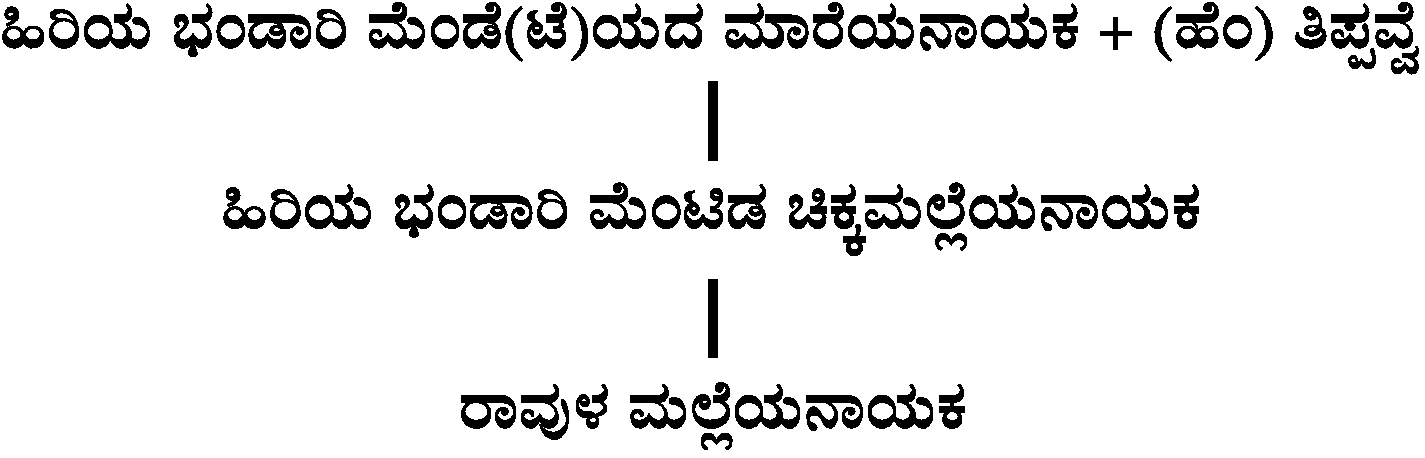
\includegraphics[scale=1.2]{images/chap3/chap3fig31.jpeg}
\end{figure}


\section*{ಹಡುವಳ\index{ಹಡುವಳ (ಹಡೆವಳ)}\enginline{-}ಹಡೆವಳ\index{ಹಡುವಳ (ಹಡೆವಳ)}\enginline{-}ಹಡಪ\index{ಹಡಪದ}}

ಪಡೆವಳ\index{ಪಡೆವಳ} ಎಂಬ ಶಬ್ದದ ಬಳಕೆಯ ರೂಪಗಳು ಹಡೆವಳ, ಹಡುವಳ, ಹಡುವಳ ಇತ್ಯಾದಿಯಾಗಿವೆ. “ಸೇನಾಧಿಕಾರಿಯೆಂದೇ ಇವುಗಳ ಅರ್ಥ. ಹಡಪವಳ\index{ಹಡಪವಳ} ಎಂಬುದು ಅರಸನಲ್ಲಿ ತಾಂಬೂಲ ಸೇವೆ ಮಾಡುವವರನ್ನು ಸೂಚಿಸುತ್ತದೆ. ಕೆಲವರು ಮನೆತನದಿಂದ ಹಡಪವಳರಾಗಿದ್ದರೂ ತಮ್ಮ ಸಾಮರ್ಥ್ಯದಿಂದ ಬೇರೆಬೇರೆ ವೃತ್ತಿ ಪಡೆದವರೂ ಆಗಿದ್ದರು. ಹಡವಪಳ ನೀಲಕಂಠನು, ದಂಡನಾಯಕ ಶ್ರೇಣಿಯ ಅಧಿಕಾರಿಯಾಗಿರಬೇಕು, ಮೂಲತಃ ಇವನು ತಾಂಬೂಲಸೇವೆಯ ಮನೆತನಕ್ಕೆ ಸಂಬಂಧಪಟ್ಟಿರಬೇಕು ಇಲ್ಲವೇ ದಂಡನಾಯಕನಾಗಿ ಬಡ್ತಿ ಹೊಂದಿರಬೇಕು” ಎಂಬ ವಿದ್ವಾಂಸರ ಅಭಿಪ್ರಾಯಗಳನ್ನು ಉಲ್ಲೇಖಿಸಬಹುದು.\endnote{ ನಾಗಯ್ಯ, ಡಾ॥ ಜೆ.ಎಂ., ಆರನೆಯ ವಿಕ್ರಮಾದಿತ್ಯನ ಶಾಸನಗಳು-ಒಂದು ಅಧ್ಯಯನ, ಪುಟ 349}

ಪಡೆ ಎಂದರೆ ಸೈನ್ಯ, ಪಡೆವಳ\index{ಪಡೆವಳ} ಎಂದರೆ ಸೇನಯ ಮುಖ್ಯಸ್ಥ ಅಥವ ಅಧಿಕಾರಿ ಎಂದು ಹೇಳಬಹುದು. ಇದರ ಅಪಭ್ರಂಶ ರೂಪಗಳೇ ಹಡುವಳ, ಹಡೆವಳ, ಹಡೆಪವಳ ಎಂಬುದಾಗಿ ತೋರುತ್ತದೆ. ‘ಪ’ ಕಾರಕ್ಕೆ ‘ಹ’ ಕಾರ ಆದೇಶವಾಗುವುದು ಸಾಮಾನ್ಯ. ಅತ್ತಿಮಬ್ಬೆಯನ್ನು\index{ಅತ್ತಿಮಬ್ಬೆ} ಪಡೆವಳ ತೈಲನ ಜನನಿ ಎಂದು ರನ್ನನು ಹೊಗಳಿದ್ದಾನೆ. ಅವಳ ಮನೆತನ ಮಂತ್ರಿಗಳು ದಂಡನಾಯಕರಿಂದ ಕೂಡಿದ ಮನೆತನ. ಅವರು ತಾಂಬೂಲಸೇವೆಯ ಕಾಯಕದಲ್ಲಿದ್ದರು ಎಂಬುದಕ್ಕೆ ಆಧಾರಗಳಿಲ್ಲ. ಹೀಗಾಗಿ ಪಡೆವಳ ಎಂದರೆ ಸೇನಾನಾಯಕರೆಂದೇ ಊಹಿಸಬಹುದು. “ಇವರು ಸೈನ್ಯದ ಸಣ್ಣಸಣ್ಣ ಪಡೆಗಳ ನಾಯಕರಾಗಿದ್ದರು. ಪಡೆವಳರ ಮೇಲಧಿಕಾರಿ ಮಹಾಪ್ರಚಂಡ ದಂಡನಾಯಕನಾಗಿರುತ್ತಿದ್ದನು. ಹಡವಳ, ಹಡಬಳ, ಈ ಹೆಸರುಗಳು ಕೆಲವೊಂದು ಸಲ ಗೊಂದಲವನ್ನು ಉಂಟುಮಾಡುತ್ತವೆ. ಆದರೆ ಇವು ಪಡೆವಳ ಎಂಬುದರ ಅನ್ಯರೂಪಗಳು".\endnote{ ನಾಗಯ್ಯ, ಡಾ॥ ಜೆ.ಎಂ., ಪಡೆವಳರು, ಹಡಪವಳರು, ಆರನೆಯ ವಿಕ್ರಮಾದಿತ್ಯನ ಶಾಸನಗಳು, ಪುಟ 347-48}

\textbf{ಹಡುವಳದ ಮಸಣೈಯ\index{ಹಡುವಳ ಮಸಣೈಯ}:} ಹೊಯ್ಸಳರ ಕಾಲದ ಸುಪ್ರಸಿದ್ಧ ಹಡುವಳರ ವಂಶವೊಂದು ನಾಗಮಂಗಲ ತಾಲ್ಲೂಕು ಹೊನ್ನೇನಹಳ್ಳಿಯಲ್ಲಿ\index{ಹೊನ್ನೇನಹಳ್ಳಿ} ಶಾಸನಗಳಲ್ಲಿ ಉಕ್ತವಾಗಿದೆ. ಹೊಯ್ಸಳ ದೇವರು (ವಿಷ್ಣುವರ್ಧನ)\index{ಹೊಯ್ಸಳ ದೇವರು (ವಿಷ್ಣುವರ್ಧನ)} ಕದಂಬರ ದಳಪತಿ ಮಸಣೈಯನ ಮೇಲೆ ಕಪಿಳೆಯ ದಡದಲ್ಲಿ\index{ಕಪಿಳೆಯ ದಡ} ಎತ್ತಿಕಟ್ಟಿದ ಯುದ್ಧದಲ್ಲಿ ಹಡುವಳದ ಮಸಣೈಯನು ಹೋರಾಡಿ ಹಲವರನ್ನು ಇರಿದು ಮಡಿಯುತ್ತಾನೆ.\endnote{ ಎಕ 7 ನಾಮಂ 105 ಹೊನ್ನೇನಹಳ್ಳಿ 12ನೇ ಶ.} ಹಡವಳದ ಬೊಟ್ಟೈಯ್ಯ\index{ಹಡವಳದ ಬೊಟ್ಟೈಯ್ಯ} (ಬೆಟ್ಟಯ್ಯ), ತಮ್ಮಯಣ್ಣ, ಇವರು ಮಸಣಯ್ಯನಿಗೆ ವೀರಗಲ್ಲನ್ನು ನಿಲ್ಲಿಸುತ್ತಾರೆ. ಹಡವಳದ ಬೊಟ್ಟೈಯ್ಯ ಮಸಣಯ್ಯನ ಮಗನಿರಬಹುದು. ಕಪಿಳೆಯ ಹೊಳೆಯು ದಕ್ಷಿಣ ಕನ್ನಡ ಜಿಲ್ಲೆಯ ಶಿಶಿಲದ ಬಳಿ ಹರಿಯುತ್ತದೆ. ಕದಂಬರೆಂದರೆ ಹಾನುಗಲ್ಲಿನ ಕದಂಬರು.

ವೀರಬಲ್ಲಾಳನ ಕಾಲದಲ್ಲಿ ಬಹುಶಃ ಇದೇ ವಂಶಕ್ಕೆ ಸೇರಿದ ಹಡುವಳದ ಹೊನ್ನಯ್ಯನು\index{ಹಡುವಳದ ಹೊನ್ನಯ್ಯ} ತುರುಗೋಳಿನಲ್ಲಿ\index{ತುರುಗೊಳ್(ಗೋಳ್), ತುರುಪ(ಪಾ)ರಿವಿ, ತುರುವಳಿವು, ತುರುಗಾಳಗ, ತುರುವ ಮಗುಳ್ಚಿ, ತುರುವನಿಕ್ಕಿಸಿ} ಹೋರಾಡಿ ಸುರಲೋಕ ಪ್ರಾಪ್ತನಾಗುತ್ತಾನೆ.\endnote{ ಎಕ 7 ನಾಮಂ 106 ಹೊನ್ನೇನಹಳ್ಳಿ 1180} ಮಹಾಸಾಮಂತ ಕುನ್ನಿಯ ಬೀರೆಯನಾಯಕನ\index{ಮಹಾಸಾಮಂತ ಕುನ್ನಿಯ ಬೀರೆಯನಾಯಕ} ಮಗ ಸಾಮಂತ ದೇಕೆಯನಾಯಕನ ಕೈಕೆಳಗೆ ಇವನು ಸೇನಾಧಿಕಾರಿಯಾಗಿದ್ದನೆಂದು ತೋರುತ್ತದೆ. ಶಾಸನವು ಹೊನ್ನಯ್ಯನನ್ನು ಸಮಸ್ತ ಪ್ರಶಸ್ತಿ ಸಹಿತ ಎಂದು, ಹಾಗೂ ಅವನ ಪತ್ನಿ ದೇಗುಲ ಗೌಣ್ಡಿಯನ್ನು\index{ದೇಗುಲ ಗೌಣ್ಡಿ} ವಿಶೇಷವಾಗಿ ಹೊಗಳಿದೆ. ಇವರ ಮಗ ಹೊನ್ನಗೌಡನು ತುರುಗೋಳಿನಲ್ಲಿ ಹಲವರನ್ನು ಇರಿದು ತುರುಗಳನ್ನು ಮರಳಿಸಿ ಸುರಲೋಕಪ್ರಾಪ್ತನಾಗುತ್ತಾನೆ. ಇವನ ಅಣ್ಣ ಮಂಚಗೌಡ\index{ಮಂಚಗೌಡ}, ತಮ್ಮಂದಿರು ಜಕ್ಕಯ್ಯ\index{ಜಕ್ಕಯ್ಯ} ಮತ್ತು ಕಲ್ಲಯ್ಯ\index{ಕಲ್ಲಯ್ಯ}(ಕಾಳಯ್ಯ) ಬೀರಗಲ್ಲನ್ನು\index{ಬೀರಗಲ್ಲು} ನಿಲ್ಲಿಸುತ್ತಾರೆ. ಹೊನ್ನಯ್ಯನಿಂದಲೇ ಈ ಊರಿಗೆ ಹೊನ್ನೇನಹಳ್ಳಿ ಎಂಬ ಹೆಸರುಬಂದಿದೆ ಎಂದು ಹೇಳಬಹುದು. ಇದೇ ಊರಿನಲ್ಲಿರುವ ವೀರಸೋಮೇಶ್ವರನ ಕಾಲದ ಇನ್ನೊಂದು ಶಾಸನದಲ್ಲಿ ಹಡವಳದೇವ ಮಲತಮ್ಮ(ಮಲ್ಲಿತಮ್ಮ)\index{ಮಲಿತಮ್ಮ(ಮಲ್ಲಿತಮ್ಮ)}, ಜಕಗೌಡನ ಬೀರಯ್ಯ\index{ಜಕಗೌಡನ ಬೀರಯ್ಯ} ಇವರುಗಳನ್ನು ಪ್ರಸ್ತಾಪಿಸುತ್ತದೆ. ಬೀರಯ್ಯನನ್ನು ಸಮಸ್ತ ಪ್ರಜೆಗೌಡಿನ ಬೀರಯ್ಯನೆಂದು\index{ಸಮಸ್ತ ಪ್ರಜೆಗೌಡಿನ ಬೀರಯ್ಯ} ಹೇಳಿದೆ.\endnote{ ಎಕ 7 ನಾಮಂ 104 ಹೊನ್ನೇನಹಳ್ಳಿ 1224} ಈ ಎಲ್ಲ ಶಾಸನಗಳಿಂದ ಇವರ ವಂಶಾವಳಿಯನ್ನು ಈ ರೀತಿ ಕಟ್ಟಿಕೊಡಬಹುದು.

\begin{figure}[H]
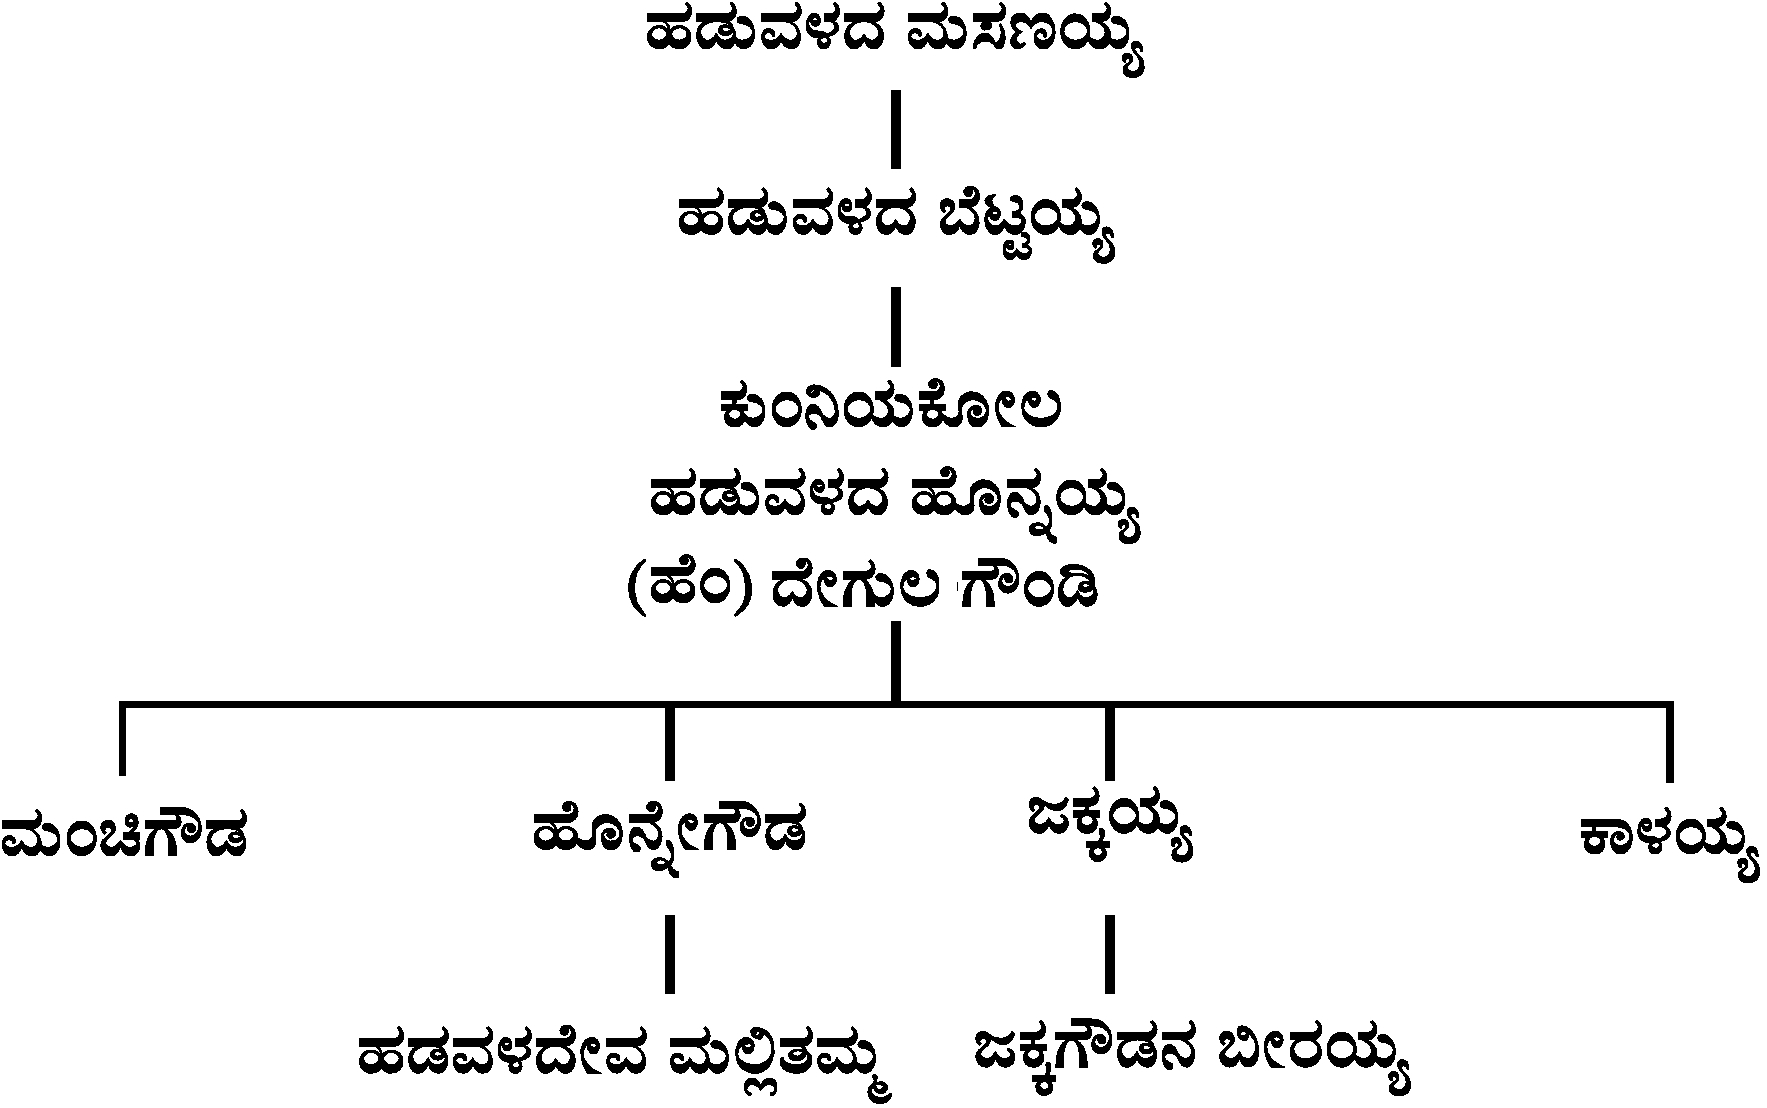
\includegraphics[scale=.15]{images/chap3/chap3fig32.jpeg}
\end{figure}

\textbf{ಹಿರಿಯ ಹಡವಳ ಕೊಳ್ಳಿ ಅಯ್ಯ\index{ಹಿರಿಯ ಹಡವಳ ಕೊಳ್ಳಿ ಅಯ್ಯ} /ಕೊಳ್ಳಿಯಮ್ಮೆಯ್ಯ\index{ಕೊಳ್ಳಿಯಮ್ಮೆಯ್ಯ}}: ಒಂದನೆಯ ನರಸಿಂಹನ ಕಾಲದಲ್ಲಿ ಹಿರಿಯ ಹಡವಳನಾಗಿದ್ದ ಕೊಳ್ಳಿಅಯ್ಯನ ಅಥವಾ ಕೊಳ್ಳಿಯಮ್ಮೆಯ್ಯನ ವಂಶಾವಳಿಯು ಕೃಷ್ಣರಾಜಪೇಟೆ ತಾಲ್ಲೂಕು ತೆಂಗಿನಘಟ್ಟ\index{ತೆಂಗಿನಘಟ್ಟ} ಶಾಸನದಲ್ಲಿ ಉಲ್ಲೇಖ\-ವಾಗಿದೆ. ಈತನು ಹಾಗೂ ಈತನ ಮಕ್ಕಳು ತೆಂಗಿನಕಟ್ಟದಲ್ಲಿ\index{ತೆಂಗಿನಘಟ್ಟ} ಹೊಯ್ಸಳೇಶ್ವರ ದೇವಾಲಯವನ್ನು\index{ಹೊಯ್ಸಳೇಶ್ವರ ದೇವಾಲಯ} ನಿರ್ಮಿಸಿ, ಕೆರೆಯನ್ನು ಕಟ್ಟಿಸಿ, ಹೊಯ್ಸಳೇಶ್ವರ ದೇವರಿಗೆ ದತ್ತಿಯನ್ನು ಬಿಡುತ್ತಾರೆ.\endnote{ ಎಕ 6 ಕೃಪೇ 42 ತೆಂಗಿನಘಟ್ಟ 1171} ಕೊಳ್ಳಿಯಮ್ಮೆಯ್ಯನ ಮಗ ಕಾಳಯ್ಯನು ಸಾಮಂತ ಪದವಿಯನ್ನು ಹೊಂದಿದ್ದನು. ಈ ಸಾಮಂತ ಕಾಳಯ್ಯನು\index{ಸಾಮಂತ ಕಾಳಯ್ಯ} ಒಂದನೆಯ ನರಸಿಂಹನು\index{ಒಂದನೆಯ ನರಸಿಂಹ} ಕೋಡಾಲದ ಬೀಡಿನಿಂದ\index{ಕೋಡಾಲದ ಬೀಡು} ಆಳುತ್ತಿದ್ದಾಗ ಯಾವುದೋ ಯುದ್ಧದಲ್ಲಿ ಹೋರಾಡಿ ಮಡಿದ ವಿಷಯ ಅಲ್ಲೆ ಇರುವ ಇನ್ನೊಂದು ವೀರಗಲ್ಲಿನಿಂದ ತಿಳಿದುಬರುತ್ತದೆ.\endnote{ ಎಕ 6 ಕೃಪೇ 43 ತೆಂಗಿನಘಟ್ಟ 12ನೇ ಶ.} ಇವರ ವಂಶಾವಳಿಯನ್ನು ಈ ರೀತಿ ನೀಡಬಹುದು.

\begin{figure}[H]
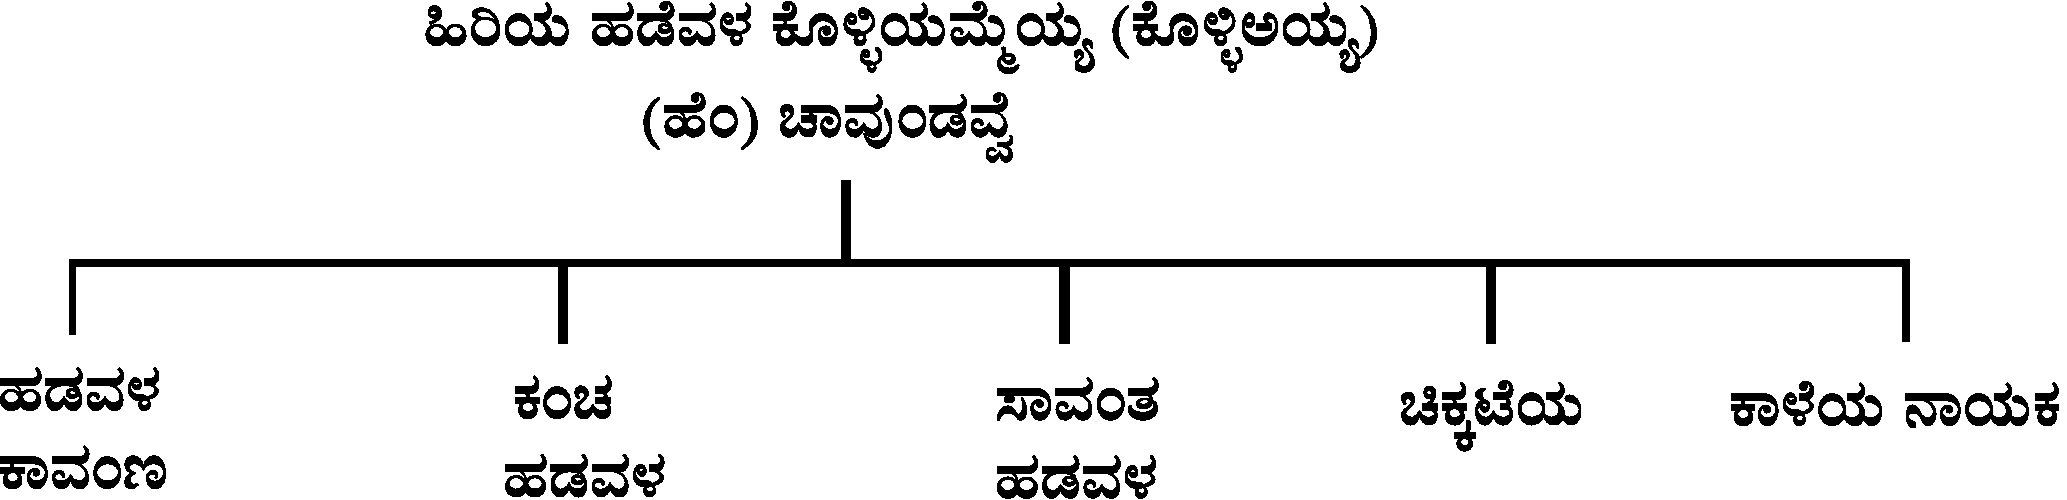
\includegraphics[scale=1.25]{images/chap3/chap3fig33.jpeg}
\end{figure}

ಹಡುವಳರು, ಸಾಮಂತ ಪದವಿಯನ್ನು ಪಡೆದು ಸೇವೆ ಸಲ್ಲಿಸುತ್ತಿದ್ದರೆಂದು ಹೇಳಬಹುದು. ಪೂರ್ವೋಕ್ತ ಹೊನ್ನೇನಹಳ್ಳಿ ಶಾಸನದಲ್ಲಿ ಬರುವ ಸಾಮಂತ ಬೀರೆಯನಾಯಕ ಅವನ ಮಗ ದೇಕೆಯನಾಯಕ ಇವರೂ ಹಡುವಳರೇ ಆಗಿದ್ದು ನಂತರ ಸಾಮಂತ ಪದವಿಯನ್ನು ಪಡೆದವರಾಗಿರಬಹುದು.

\textbf{ಹಡಪದ ಸಾಯಣ್ಣ\index{ಹಡಪದ ಸಾಯಣ್ಣ}:} ಮೂರನೆಯ ಬಲ್ಲಾಳನ ಕಾಲದಲ್ಲಿದ್ದ ಹಡಪದ ಸಾಯಣ್ಣನು, ತನ್ನ ಒಡೆಯ ಚಿಮ್ಮತ್ತೂರಕಲ್ಲ ಸೋಮೆಯ ದಂಡನಾಯಕನ ಜೊತೆ ಹೊಳಲಕೆರೆಯಲ್ಲಿ\index{ಹೊಳಲಕೆರೆ} ಕಂಪಿಲನ\index{ಕಂಪಿಲ} ವಿರುದ್ಧ ಹೋರಾಡುವಾಗ ವೊಡೆಯರಕೂಡೆ ಹೋರಾಡಿ ಮೃತಪಟ್ಟನೆಂದು ಕೃಷ್ಣರಾಜಪೇಟೆ ತಾಲ್ಲೂಕು ಚಿಟ್ಟನಹಳ್ಳಿ\index{ಚಿಟ್ಟನ ಹಳ್ಳಿ} ವೀರಗಲ್ಲಿನಿಂದ ತಿಳಿದುಬರುತ್ತದೆ.\endnote{ ಎಕ 6 ಕೃಪೇ 100 ಚಿಟ್ಟನಹಳ್ಳಿ 1303 ಏಪ್ರಿಲ್​ 18} ಇದು ಮೂರನೆಯ ಬಲ್ಲಾಳ ಮತ್ತು ಅವನ ಮಹಾಪ್ರಧಾನ ದಂಡನಾಯಕ ಸೋಮಯೆ ದಂಣಾಯಕ\index{ಸೋಮಯೆ ದಂಣಾಯಕ} ಇವರು ಕಂಪಿಲದೇವನೊಡನೆ ನಡೆಸಿದ ಯುದ್ಧವಾಗಿರುತ್ತದೆ. ಈ ಶಾಸನದಲ್ಲಿ ಸೋಮೆಯ ದಂಡನಾಯಕ ಮತ್ತು ಹಡಪದ ಸಾಯಣ್ಣ ಈ ಇಬ್ಬರೂ ವೊಡೆಯರ ಕೂಡೆ ಕಾದಿದರೆಂದು ಹೇಳಿರುವುದರಿಂದ ಮುಮ್ಮಡಿ ಬಲ್ಲಾಳನೂ ಕೂಡಾ ಈ ಯುದ್ಧದಲ್ಲಿ ಭಾಗವಹಿಸಿದ್ದನೆಂದು ಹೇಳಬಹುದು. ಹಡಪದ ಸಾಯಣ್ಣನು \textbf{“ಗಂಡಪೆಂಡಾರಗೊಂಡನೆಂದು\index{ಗಂಡಪೆಂಡಾರ} ಮರಳಿಬಿಟ್ಟು ಹೊಯಿದು ಹೊಯಿದು ಕಾದಿ ಬಿದ್ದನೆಂದು”} ಶಾಸನ ವರ್ಣಿಸಿದೆ. ಹಡಪದ ಸಾಯಣ್ಣನು ಚಿಟ್ಟನಹಳ್ಳಿಯ\index{ಚಿಟ್ಟನ ಹಳ್ಳಿ} ಕಾಮಗವುಡನ ಮಗ ಹಿರಿಯತಮ್ಮನ ಮಗ ಬೀಮಣ್ಣನ ತಮ್ಮನೆಂದು ಹೇಳಿದೆ. ಇವನ ವಂಶಾವಳಿಯನ್ನು ಈ ರೀತಿ ಸೂಚಿಸಬಹುದು. ಇವರು ಯಾವುದೋ ಕುಲಕ್ಕೆ (ಸಂ...ಕ ಕುಲಕೆ ತಿಲಕರು) ಸೇರಿದವರೆಂದು ಹೇಳಿದ್ದು ಅದು ತ್ರುಟಿತವಾಗಿದೆ. ಇದು ಸಂಕಿಯರ ಕುಲ\index{ಸಂಕಿಯರ ಕುಲ} ಇರಬಹುದು. ಇವರ ವಂಶಾವಳಿ.

\begin{figure}[H]
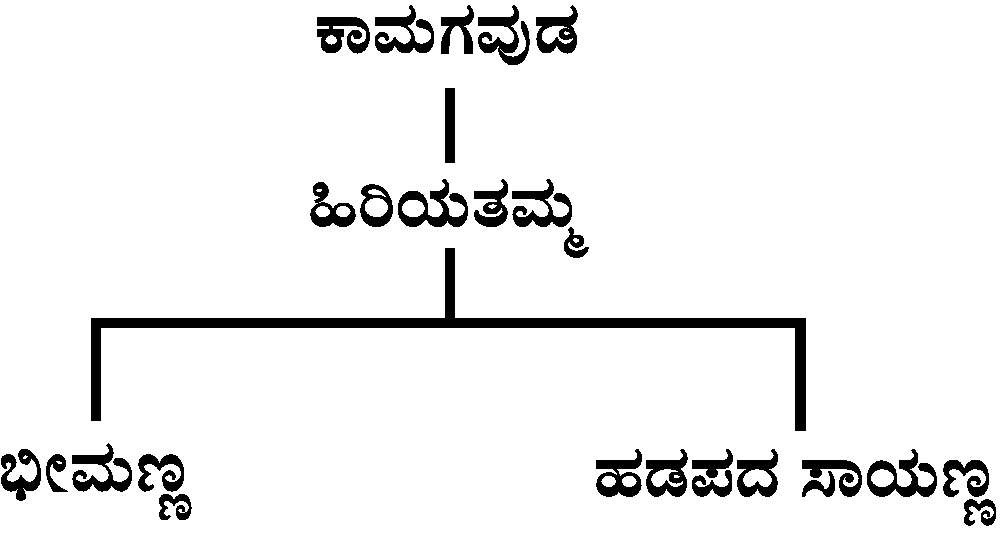
\includegraphics[scale=1.2]{images/chap3/chap3fig34.jpeg}
\end{figure}


\section*{ಪೆರ್ಗ್ಗಡೆ\index{ಪೆರ್ಗ್ಗಡೆ}/ಹಿರಿಯ ಹೆಗ್ಗಡೆಗಳು\index{ಹಿರಿಯ ಹೆಗ್ಗಡೆಗಳು}}

ಪೆರ್ಗ್ಗಡೆ ಅಥವಾ ಹಿರಿಯ ಹೆಗ್ಗಡೆಗಳು ಆಡಳಿತದ ಕೆಳಹಂತದಲ್ಲಿ ಅತ್ಯಂತ ಪ್ರಮುಖ ಅಧಿಕಾರಿಗಳಾಗಿದ್ದರು. ಇವರಲ್ಲಿ \textbf{ಸುಂಕದ ಹೆಗ್ಗಡೆ\index{ಸುಂಕದ ಹೆಗ್ಗಡೆ}, ಮನೆ ವೆಗ್ಗಡೆ (ಅರಮನೆಯ ಹೆಗ್ಗಡೆ)\index{ಮನೆ ವೆಗ್ಗಡೆ (ವೆರ್ಗ್ಗಡೆ) (ಅರಮನೆಯ ಹೆಗ್ಗಡೆ)}, ಹಿರಿಯಹೆಗ್ಗಡೆ, ಕೊಟ್ಟರವೆಗ್ಗಡೆ\index{ಕೊಟ್ಟರವೆಗ್ಗಡೆ}, ಆಯತದ ಹೆಗ್ಗಡೆ\index{ಆಯತದ ಹೆಗ್ಗಡೆ} ಎಂದು ಅನೇಕ ರೀತಿಯ ಅಧಿಕಾರ ಸ್ಥಾನಗಳಿದ್ದುದು ಶಾಸನಗಳಿಂದ ತಿಳಿದುಬರುತ್ತದೆ. } ಇವರು ನಿರ್ವಹಿಸುವ ಇಲಾಖೆಗೆ ಸಂಬಂಧಿಸಿದಂತೆ ಇವರಿಗೆ ಈ ಪದವಿಗಳು ಪ್ರದಾನವಾಗಿದ್ದವು. ಅನೇಕ ಶಾಸನಗಳಲ್ಲಿ ಇವರನ್ನು ಹೆಗ್ಗಡೆ ಎಂದು ಕರೆಯಲಾಗಿದ್ದು, ಇವರ ಯಾವ ಇಲಾಖೆಯನ್ನು ನಿರ್ವಹಿಸುತ್ತಿದ್ದರು ಎಂಬುದು ತಿಳಿದುಬರುವುದಿಲ್ಲ. ಕೆಲವು ಹೆಗ್ಗಡೆಗಳು ತಮ್ಮ ಶಕ್ತಿಸಾಮರ್ಥ್ಯ, ದಕ್ಷತೆಗಳಿಂದ ಹಿರಿಯಹೆಗ್ಗಡೆ ಎಂದು ಕರೆಯಿಸಿಕೊಂಡು ಮಹಾಪ್ರಧಾನ ಪದವಿಗೆ ಏರಿದ್ದರೆಂದು ಹೇಳಬಹುದು. “ಪೆರ್ಗ್ಗಡೆ ಎಂಬುದು ಸಂಸ್ಕೃತದ ಮಹತ್ತರ ಎಂಬುದರ ಸಮಾನರೂಪ ಎಂದು ಹೇಳಿ ಇವೆರಡೂ ದೊಡ್ಡ ಅಧಿಕಾರಿಗಳನ್ನು ಸೂಚಿಸುವ ಪದಗಳು” ಎಂದು ಚಿದಾನಂದಮೂರ್ತಿಯವರು ಹೇಳಿದ್ದಾರೆ.\endnote{ ಚಿದಾನಂದಮೂರ್ತಿ ಡಾ॥ ಎಂ, ಕನ್ನಡ ಶಾಸನಗಳ ಸಾಂಸ್ಕೃತಿಕ ಅಧ್ಯಯನ, ಪುಟ 103, 111} ಹೆಗ್ಗಡೆ ಮತ್ತು ಪೆರ್ಗ್ಗಡೆ ಒಂದೇ ಎಂದು ಅಭಿಪ್ರಾಯ ಪಟ್ಟಿರುವ ದೀಕ್ಷಿತ್​ ಅವರು ಗಾವುಂಡ ಮತ್ತು ಪೆರ್ಗಡೆ ಎಂಬುವರು ನಾಡುಗಳ ಇಲ್ಲವೇ ಹಳ್ಳಿಗಳ ಯಾವುದೇ ವಿಭಾಗದ ಮುಖ್ಯಸ್ಥರಾಗಿರುತ್ತಿದ್ದರು. ಪೆರ್ಗಡೆಯು ಸುಂಕವನ್ನು ಸಂಗ್ರಹಿಸುವ ಅಧಿಕಾರ ಹೊಂದಿರುತ್ತಿದ್ದರೆ ಅವನು ಸುಂಕದ ಪೆರ್ಗಡೆಯಾಗಿರುತ್ತಿದ್ದನು, ಶ‍್ರೀಕರಣದ ಅಧಿಕಾರ ಹೊಂದಿದ್ದರೆ ಶ‍್ರೀಕರಣ ಪೆರ್ಗಡೆ(ಹೆಗ್ಗಡೆ)\index{ಶ‍್ರೀಕರಣ ಪೆರ್ಗಡೆ(ಹೆಗ್ಗಡೆ)} ಯಾಗಿರುತ್ತಿದ್ದನು ಎಂದು ಹೇಳಿದ್ದಾರೆ.\endnote{ \engfoot{Dixit, G.S., Local Self Government in Mediaeval Karnataka, P.37}} ನಾಗಯ್ಯನವರೂ ಪೆರ್ಗಡೆ ಮತ್ತು ಹೆಗ್ಗಡೆ ಇಬ್ಬರನ್ನೂ ಒಂದೇ ಎಂಬುದಾಗಿ ಹೇಳುತ್ತಾರೆ. “ಆರನೆಯ ವಿಕ್ರಮಾದಿತ್ಯನ ಕಾಲದ ಶಾಸನೋಕ್ತ ಹೆಗ್ಗಡೆಗಳೆಲ್ಲರೂ ಸುಂಕಕ್ಕೆ ಮಾತ್ರ ಸಂಬಂಧಪಟ್ಟವರಾಗಿದ್ದಾರೆ. ಇವರಾರೂ ಒಟ್ಟು ಆಡಳಿತ ನೋಡಿಕೊಂಡು ಹೋಗುತ್ತಿದ್ದ ಉಲ್ಲೇಖ ದೊರೆಯುವುದಿಲ್ಲ” ಎಂದು ಹೇಳಿದ್ದಾರೆ.\endnote{ ನಾಗಯ್ಯ ಡಾ. ಜೆ.ಎಂ., ಆರನೆಯ ವಿಕ್ರಮಾದಿತ್ಯನ ಶಾಸನಗಳು- ಒಂದು ಅಧ್ಯಯನ, ಪುಟ 350-353} ಕೋರವಂಗಲ ಶಾಸನದಲ್ಲಿ ಪೆರ್ಗ್ಗಡೆ ಗೋವಿಂದನನ್ನು ಹೆಗ್ಗಡೆ ಗೋವಿಂದ ಎಂದು ಕರೆದಿರುವುದರಿಂದ ಪೆರ್ಗಡೆ, ಹೆಗ್ಗಡೆ ಒಂದೇ ಎಂದು ಹೇಳಬಹುದು.\endnote{ ಎಕ 8 ಹಾಸನ 129 ಕೋರವಂಗಲ 1160} ಪಂಪಭಾರತದಲ್ಲಿ ಶಂತನುವು “ದಾಶರಾಜನಲ್ಲಿಗೆ ಕೂಸಂ ಬೇಡೆ ಪೆರ್ಗ್ಗಡೆಗಳನ್ನು” ಅಟ್ಟಿದನೆಂದು, ದುರ್ಯೋಧನನು “ತನ್ನ ಮನದನ್ನನಪ್ಪ ಪೆರ್ಗಡೆಯೊಳ್​ ಲಾಕ್ಷಾಗೃಹೋಪಾಯಮುಂ ಚಿಂತಿಸಿದನೆಂದು” ಹೇಳಿದೆ.\endnote{ ಪಂಪ ಭಾರತ, ಆಶ್ವಾಸ 1-70, ಆಶ್ವಾಸ 1-92} ಇದರಿಂದ ಅರಮನೆಯಲ್ಲಿಯೂ ಪೆರ್ಗ್ಗಡೆಗಳು ಇದ್ದು ರಾಜಕಾರ್ಯ ನಿರ್ವಹಿಸುತ್ತಿದ್ದರೆಂದು ತಿಳಿದುಬರುತ್ತದೆ.

ಹೆಗ್ಗಡೆಗಳು, ಅಗ್ರಹಾರಗಳಲ್ಲಿ, ಊರುಗಳಲ್ಲಿ ಅಥವಾ ಪಟ್ಟಣಗಳಲ್ಲಿ ವಾಸಮಾಡಿಕೊಂಡು, ಅಲ್ಲಿನ ಹಾಗೂ ಸುತ್ತಮುತ್ತಲ ಪ್ರದೇಶದ ಆಡಳಿತವನ್ನು ನೋಡಿಕೊಳ್ಳುತ್ತಿದ್ದರೆಂದು ಹೇಳಬಹುದು. ಮುಖ್ಯವಾಗಿ ತೆರಿಗೆ ಮತ್ತು ಸುಂಕಗಳ ಮೇಲೆ ಇವರ ಆಡಳಿತ ಇರುತ್ತಿದ್ದುದು ಕಂಡು ಬರುತ್ತದೆ. ಸುಂಕ ಮತ್ತು ತೆರಿಗೆಗಳನ್ನು ನಿಗದಿಪಡಿಸಿ, ಅದನ್ನು ವಸೂಲು ಮಾಡುವುದು, ಅವುಗಳಿಗೆ ರಿಯಾಯಿತಿ ನೀಡುವುದು, ಭೂಮಿಯ ಮೇಲಿನ ಹಕ್ಕು ರಕ್ಷಣೆ, ಭೂಮಿಗಳನ್ನು ದತ್ತಿಬಿಡುವುದು ಈ ಕಾರ್ಯಗಳನ್ನು ನಿರ್ವಹಿಸುತ್ತಿದ್ದುದು ಜಿಲ್ಲೆಯ ಶಾಸನಗಳ ಅಧ್ಯಯನದಿಂದ ಕಂಡುಬರುತ್ತದೆ. ಕೆಲವು ವೇಳೆ ಸ್ವತಂತ್ರವಾಗಿ ಮತ್ತೆ ಕೆಲವೊಮ್ಮೆ ಮಹಾಪ್ರಧಾನರು, ಅರಸರ ಅಪ್ಪಣೆಯ ಮೇರೆಗೆ ಇವರು ದತ್ತಿಗಳನ್ನು ಬಿಡುತ್ತಿದ್ದರು. ಇವರು ದೇವಾಲಯಗಳನ್ನು ನಿರ್ಮಿಸಿ ಕೆರೆಕಟ್ಟೆಗಳನ್ನು ಕಟ್ಟಿಸಿದ ಅನೇಕ ಉದಾಹರಣೆಗಳೂ ಇವೆ.

\textbf{ಪೆರ್ಗ್ಗಡೆ ಮಲ್ಲಿಯಣ್ಣ\index{ಪೆರ್ಗ್ಗಡೆ ಮಲ್ಲಿಯಣ್ಣ}:} ವಿನಯಾದಿತ್ಯನ ಕಾಲದಲ್ಲಿ ಪೆರ್ಗ್ಗಡೆ ಮಲ್ಲಿಯಣ್ಣನು ಸ್ವಧರ್ಮದಿಂದ ದೇವಾಲಯವನ್ನು ಮಾಡಿಸಿ, ಕನ್ನೆಗೆರೆಯನ್ನು\index{ಕನ್ನೆಗೆರೆ} ಕಟ್ಟಿಸಿ, ಬ್ರಹ್ಮೇಶ್ವರ\index{ಬ್ರಹ್ಮೇಶ್ವರ} ದೇವರಿಗೆ ದತ್ತಿಯಾಗಿ ಬಿಟ್ಟನು.\endnote{ ಎಕ 6 ಕೃಪೆ 37 ಕಿಕ್ಕೇರಿ 1095-96} ಮಲ್ಲಿಯಣ್ಣನು ತೆರಿಗೆ ಹಣದಿಂದ ದೇವಾಲಯವನ್ನು ನಿರ್ಮಿಸಿ, ಕೆರೆಯನ್ನು ಕಟ್ಟಿಸುವ ಅಧಿಕಾರ ಹೊಂದಿದ್ದರೂ, “ಸ್ವಧರ್ಮದಿಂದ\index{ಸ್ವಧರ್ಮ}” ಅಂದರೆ ಸ್ವಂತ ಸಂಪಾದನೆ\-ಯಿಂದ ಇವುಗಳನ್ನು ಮಾಡಿದನು ಎಂದು ಹೇಳಬಹುದು. ಮಲ್ಲಿಯಣ್ಣನು ಶೈವಯತಿ ಬ್ರಹ್ಮರಾಶಿ ಪಂಡಿತನ\index{ಬ್ರಹ್ಮರಾಶಿ ಪಂಡಿತ} ಮಗ(ಶಿಷ್ಯ)\-ನಾದ್ದರಿಂದ ಈ ದೇವರಿಗೆ ಬ್ರಹ್ಮೇಶ್ವರ ದೇವರೆಂಬ ಹೆಸರನ್ನು ಇಡುತ್ತಾನೆ. ಕಿಕ್ಕೇರಿಯ ಊರೊಳಗಿನ ಕೆಲವು ತೆರಿಗೆಗಳನ್ನು ಕೂಡಾ ಈ ದೇವಾಲಯಕ್ಕೆ ದತ್ತಿ ಬಿಟ್ಟಂತೆ ತಿಳಿದುಬರುತ್ತದೆ. ಈಗ ಕಿಕ್ಕೇರಿ ಕೆರೆ ಏರಿಯ ಹಿಂದೆ ಇರುವ ಪಾಳು ಮಲ್ಲೇಶ್ವರ ದೇವಾಲಯವೇ ಮಲ್ಲಿಯಣ್ಣ ಕಟ್ಟಿಸಿದ ದೇವಾಲಯವಾಗಿದೆ. ಇದನ್ನು ಮೂಲಸ್ಥಾನ ಬ್ರಹ್ಮೇಶ್ವರ\index{ಮೂಲಸ್ಥಾನ ಬ್ರಹ್ಮೇಶ್ವರ} ದೇವರು ಎಂದು ಹೇಳಿದ್ದು ಇದಕ್ಕೆ ಬಿಟ್ಟಿಯ ದೇವನು ಗದ್ದೆಯನ್ನು ಮತ್ತು ಬೂವನಹಳ್ಳಿಯನ್ನು\index{ಬೂವನಹಳ್ಳಿ} ಧಾರಾಪೂರ್ವಕವಾಗಿ ಬಿಟ್ಟನೆಂದು ಹೇಳಿದೆ.

\textbf{ಪೆರಾಳ್ಕೆ ಹೆಗ್ಗಡೆ ಚಂದಯ್ಯ\index{ಪೆರಾಳ್ಕೆ ಹೆಗ್ಗಡೆ ಚನ್ದಯ್ಯ}:} ಪೆರಾಳ್ಕೆ ಹೆಗ್ಗಡೆ ಚಂದಯ್ಯನು ತೊಳಂಚೆಯ ಅಂಕಕಾರ\index{ತೊಳಂಚೆಯ ಅಂಕಕಾರ} ದೇವರಿಗೆ ದೇವಪರ್ವ ನಿಮಿತ್ತ ದತ್ತಿ ಬಿಟ್ಟು ಅದನ್ನು ಮಹಾದೇಸಿಗರು\index{ಮಹಾದೇಸಿಗರು} ನಡೆಸಿಕೊಡಬೇಕೆಂದು ಹೇಳುತ್ತಾನೆ. ಪೆರಾಳ್ಕೆ ಎಂಬುದು “ಪಿರಿಯ+ಆಳ್ವಿಕೆ” ಎಂಬುದರಿಂದ ಬಂದಿರಬಹುದು. “ಮಹಾಸಾಮಂತ ದೇಕೆಯನಾಯಕರ\index{ಮಹಾಸಾಮಂತ ದೇಕೆಯನಾಯಕ} ಮೇಲಾಳಿಕೆ\index{ಮೇಲಾಳಿಕೆ}” ಎಂಬುದಾಗಿ ಹೊನ್ನೇನಹಳ್ಳಿ\index{ಹೊನ್ನೇನಹಳ್ಳಿ} ಶಾಸನದಲ್ಲಿದೆ.\endnote{ ಎಕ 7 ನಾಮಂ 106 ಹೊನ್ನೇನಹಳ್ಳಿ 1180} ಮೇಲಾಳಿಕೆ ಮೈಮೆಟ್ಟಿ, ಮೇಲಾಳಿಕೆ ಸಾವಿಯಣ್ಣ\index{ಮೇಲಾಳಿಕೆ ಸಾವಿಯಣ್ಣ} ಇವರುಗಳ ಪ್ರಸ್ತಾಪ ಗಿಜಿಹಳ್ಳಿ ಶಾಸನದಲ್ಲಿ ಬರುತ್ತದೆ.\endnote{ ಎಕ 10 ಚರಾಪ 222 ಗಿಜಿಹಳ್ಳಿ 1200} ಪೇರಾಳ್ಕೆ, ಮೇಲಾಳಿಕೆ ಎರಡೂ ಒಂದೇ ಆಗಿದ್ದು, ಇವರು ಗ್ರಾಮ ಅಥವಾ ಗ್ರಾಮಗಳ ಆಡಳಿತದ ಮೇಲ್ವಿಚಾರಣೆ ಮಾಡುತ್ತಿದ್ದರೆಂದು ಹೇಳಬಹುದು.

\textbf{ಪೆರ್ಗ್ಗಡೆ ಮಲ್ಲಿನಾಥ\index{ಪೆರ್ಗ್ಗಡೆ ಮಲ್ಲಿನಾಥ}:} ವಿಷ್ಣುವರ್ಧನನ ಕಾಲದಲ್ಲಿ ಪೆರ್ಗ್ಗಡೆ ಮಲ್ಲಿನಾಥನು, ಬಹುಶಃ ಮಲ್ಲಘಟ್ಟದಲ್ಲಿ\index{ಮಲ್ಲಘಟ್ಟ} (ಇಂದಿನ ಅಬಲವಾಡಿಯಲ್ಲಿ\index{ಅಬಲವಾಡಿ}) ಮಲ್ಲಿನಾಥ ಬಸದಿಯನ್ನು ನಿರ್ಮಿಸಿ, ವಿಷ್ಣುವರ್ಧನನ\index{ವಿಷ್ಣುವರ್ಧನ (ದೇವರು) (ಹೊಯ್ಸಳರ ದೊರೆ)} ಅನುಮತಿಯಿಂದ ಅದಕ್ಕೆ, ಗದ್ದೆಯನ್ನು, ಮಲ್ಲಘಟ್ಟ ಗ್ರಾಮವನ್ನು ದತ್ತಿಯಾಗಿ ಬಿಡಿಸಿದನೆಂದು ಇಲ್ಲಿರುವ ತ್ರುಟಿತ ಶಾಸನದಿಂದ ಊಹಿಸಬಹುದು. ಇದನ್ನು “ಶ‍್ರೀಯುಳ್ಳಿನ ಬಸದಿ\index{ಶ‍್ರೀಯುಳ್ಳಿನ ಬಸದಿ}” ಎಂದು ಕರೆಯಲಾಗಿದೆ. ಮಲ್ಲಿನಾಥನ ತಂದೆ ಭೀಮ\index{ಭೀಮ}, ತಾಯಿ ಮಾಚಿಕೆ\index{ಮಾಚಿಕೆ}, ಗುರುಗಳು ನಯಕೀರ್ತಿ\index{ನಯಕೀರ್ತಿ} ಮತ್ತು ಭಾನುಕೀರ್ತಿ\index{ಭಾನುಕೀರ್ತಿ ದೇವ (ಮುನೀಂದ್ರ)} ಮುನಿಗಳು ಎಂದು ತಿಳಿದುಬರುತ್ತದೆ.\endnote{ ಎಕ 7 ಮ 29 ಅಬಲವಾಡಿ 1131} ಈತನು ಮುಂದೆ ಸಂಧಿವಿಗ್ರಹಿ\index{ಸಂಧಿವಿಗ್ರಹಿ} ಪದವಿಗೆ ಏರಿದನು. “ಭಾನುಕೀರ್ತಿದೇವರ\index{ಭಾನುಕೀರ್ತಿ ದೇವ (ಮುನೀಂದ್ರ)} ಗುಡ್ಡ ಸಂಧಿವಿಗ್ರಹಿ ಮಲ್ಲಿಯಣ್ಣ ನಿಶಿಧಿಯಂ ಮಾಡಿಸಿ ಪ್ರತಿಷ್ಠೆ ಮಾಡಿದಂ” ಎಂದು ಶ್ರವಣಬೆಳಗೊಳದ ಶಾಸನದಿಂದ ತಿಳಿದುಬರುತ್ತದೆ.\endnote{ ಎಕ 2 ಶ್ರವಣಬೆಳಗೊಳ 81 ಚಿಕ್ಕಬೆಟ್ಟ 12ನೇ ಶ.} ಮಲ್ಲಘಟ್ಟದ ಹೆಸರು ಮಲ್ಲಿನಾಥ ಘಟ್ಟ\index{ಮಲ್ಲಿನಾಥ ಘಟ್ಟ} ಎಂದು ಇರಬಹುದು. ಶ‍್ರೀಯುಳ್ಳಿನ ಬಸದಿಯು ಮಲ್ಲಿನಾಥ ಬಸದಿಯಾಗಿರಬಹುದು. ಮುಂದೆ ಶ‍್ರೀವೈಷ್ಣವ ಧರ್ಮದ ಪ್ರಭಾವದ ಕಾಲಕ್ಕೆ ಇದು ಅಹೋಬಲವಾಡಿ\index{ಅಹೋಬಲವಾಡಿ} (ಅಬಲವಾಡಿ) ಆಗಿರಬಹುದು. ಅಬಲವಾಡಿಯಲ್ಲಿ ಈಗ ನರಸಿಂಹ ದೇವಾಲಯವಿದೆ.

\textbf{ಪೆರ್ಗ್ಗಡೆ ಕೊಮ್ಮಣ್ಣ\index{ಪೆರ್ಗ್ಗಡೆ ಕೊಮ್ಮಣ್ಣ}:} ಮಹಾಪ್ರಧಾನ ದಂಡನಾಯಕ ಸುರಿಗೆ ನಾಗಯ್ಯನ ಆದೇಶದ ಮೇರೆಗೆ ಪೆರ್ಗ್ಗಡೆ ಕೊಮ್ಮಣ್ಣನು “ಮುಂಡಿಗೈ ತರೈ” ಎಂದರೆ ಮಗ್ಗದ ತೆರಿಗೆಯನ್ನು ಕೇಶವ ದೇವರಿಗೆ ದತ್ತಿಯಾಗಿ ಬಿಡುತ್ತಾನೆ.\endnote{ ಎಕ 6 ಶ‍್ರೀಪ 104 ಅರಕೆರೆ 12ನೇ ಶ.} ಹೆಗ್ಗಡೆ ಕೊಮ್ಮಣ್ಣ\index{ಹೆಗ್ಗಡೆ ಕೊಮ್ಮಣ್ಣ} ಮತ್ತು ಹೆಗ್ಗಡೆ ಕೇಶಿಯಣ್ಣ\index{ಹೆಗ್ಗಡೆ ಕೇಶಿಯಣ್ಣ} ಇವರುಗಳು ಶ‍್ರೀಮನ್​ ಮಹಾಪ್ರಧಾನ ಸರ್ವಾಧಿಕಾರಿ ದಂಡದಧಿಷ್ಠಾಯಕ\index{ದಂಡದಧಿಷ್ಠಾಯಕ} ಮಹಾಪಸಾಯ್ತ\index{ಮಹಾ ಪಸಾಯ್ತ (ಪಸಾಯಿತ, ಪಸಾಯತ)ರು} ಹಿರಿಯ ಹೆಗ್ಗಡೆ ಮಾಚಯ್ಯ\index{ಹಿರಿಯ ಹೆಗ್ಗಡೆ ಮಾಚಯ್ಯ} ಇವನ ಮಕ್ಕಳಾಗಿದ್ದ ವಿಚಾರ ತೊಣ್ಣೂರು ಶಾಸನದಿಂದ ತಿಳಿದುಬರುತ್ತದೆ.\endnote{ ಎಕ 6 ಪಾಂಪು 63 ತೊಣ್ಣೂರು 1174} ಪೂರ್ವೋಕ್ತ ಅರಕೆರೆ ಶಾಸನದ ಕಾಲಕ್ಕೆ ಕೊಮ್ಮಣ್ಣನು ಪೆರ್ಗ್ಗಡೆ ಅಂದರೆ ಹಿರಿಯ ಹೆಗ್ಗಡೆ ಪದವಿಗೆ ಏರಿದ್ದನು.

\textbf{ವಿಟ್ಟಿಯಣ್ಣ ಪೆರ್ಗ್ಗಡೆ\index{ವಿಟ್ಟಿಯಣ್ಣ ಪೆರ್ಗ್ಗಡೆ}:} ಒಂದನೆಯ ನರಸಿಂಹನ ಕಾಲದಲ್ಲಿ ವಿಟ್ಟಿಯಣ್ಣ ಪೆರ್ಗ್ಗಡೆಯು, ಮದ್ದೂರು ನರಸಿಂಹ ಸ್ವಾಮಿ ದೇವಾಲಯದಲ್ಲಿರುವ, ನಾಚ್ಚಿಯಾರ್​ಗೆ ಮೂರು ಹೊನ್ನು ಕಚ್ಚಾಣ(ಗದ್ಯಾಣ)ವನ್ನು ದತ್ತಿಯಾಗಿ ಬಿಟ್ಟನೆಂದು, ತ್ರುಟಿತ ತಮಿಳು ಶಾಸನದಿಂದ ತಿಳಿದುಬರುತ್ತದೆ.\endnote{ ಎಕ 7 ಮ 3 ಮದ್ದೂರು 1151-52}

\textbf{ನಾಯಕ ಹೆಗ್ಗಡೆ\general{\enginline{-}}ತಿಲೆನಾಯಕ ಹೆಗ್ಗಡೆ\index{ತಿಲೆನಾಯಕ ಹೆಗ್ಗಡೆ}:} ನಾಯಕ ಹೆಗ್ಗಡೆ ಹುದ್ದೆಯು ಹಿರಿಯಹೆಗ್ಗಡೆ ಅಥವಾ ಪೆರ್ಗ್ಗಡೆಗೆ ಸಮಾನವಾದ ಹುದ್ದೆಯೆಂದು ಹೇಳಬಹುದು. \textbf{“ತಿಲೆ ನಾಯಕ ಹೆಗ್ಗಡೆಯರು ಬಿನ್ನಪಂ ಗೈಯಲು ಶ‍್ರೀನಾರಸಿಂಹದೇವರು\index{ಶ‍್ರೀನಾರಸಿಂಹದೇವರು}”} ಕಿಕ್ಕೇರಿಯ ಬ್ರಹ್ಮೇಶ್ವರ\index{ಬ್ರಹ್ಮೇಶ್ವರ} ದೇವರಿಗೆ ಬೂವನಹಳ್ಳಿಯನ್ನು ದತ್ತಿಯಾಗಿಬಿಟ್ಟರೆಂದು ಹೇಳಿದೆ.\endnote{ ಎಕ 6 ಕೃಪೇ 27 ಕಿಕ್ಕೇರಿ 1171} ತಿಲೆ ಎಂಬುದರ ಅರ್ಥ ಸ್ಪಷ್ಟವಿಲ್ಲ.

\textbf{ನಾಯಕ ಹೆಗ್ಗಡೆ ಮಾರಣ್ಣ\index{ನಾಯಕ ಹೆಗ್ಗಡೆ ಮಾರಣ್ಣ}:} ನಾಯಕ ಹೆಗ್ಗಡೆ ಮಾರಣ್ಣನು ಮಹಾಪ್ರಧಾನ ಸರ್ವಾಧಿಕಾರಿ ಮಹಾಪಸಾಯತ,\break ತಂತ್ರಾಧಿಷ್ಟಾಯಕ ಹೆಗ್ಗಡೆ ಸುರಿಗೆಯ ನಾಗಣ್ಣನ\index{ಸುರಿಗೆಯ (ಸುರಗಿಯ) ನಾಗಯ್ಯ (ನಾಗಿದೇವ, ನಾಗಣ್ಣ)} ಬೆಸದಿಂದ, ತೊಂಡನೂರ\index{ತೊಂಡನೂರ} ನಡುವಣ ದೇವಾಲಯಕ್ಕೆ\index{ನಡುವಣ ದೇವಾಲಯ} ಇನ್ನೂರು ಎಲೆಯಗುಳಿ\-ಯನ್ನು\index{ಎಲೆಯಗುಳಿ}, ಇನ್ನೂರೆಂಬತ್ತು ಎಲೆಯ ಗುಳಿಯ \textbf{ಪಂನಾಯವನ್ನು\index{ಪಂನಾಯ} ಸರ್ವಬಾಧಾಪರಿಹಾರವಾಗಿ} ದತ್ತಿ ಬಿಡುತ್ತಾನೆ.\endnote{ ಎಕ 6 ಪಾಂಪು 79 ತೊಣ್ಣೂರು 1175}

\vskip -3pt

\section*{ಹೆಗ್ಗಡೆಗಳು\index{ಹೆಗ್ಗಡೆಗಳು}}

ಹೆಗ್ಗಡೆಗಳು ಹಿರಿಯಹೆಗ್ಗಡೆ ಅಥವಾ ಪೆರ್ಗ್ಗಡೆಗಳ ಕೆಳಗಿನ ಅಧಿಕಾರಿಗಳಾಗಿದ್ದರೆಂದು ಹೇಳಬಹುದು. ಪೆರ್ಗ್ಗಡೆ, ಹೆಗ್ಗಡೆ ಎರಡೂ ಒಂದೇ ಪದವಿ ಎಂದು ವಿದ್ವಾಂಸರು ಹೇಳಿದ್ದಾರೆ.\endnote{ ಚಿದಾನಂದಮೂರ್ತಿ, ಡಾ॥ ಎಂ., ಕನ್ನಡ ಶಾಸನಗಳ ಸಾಂಸ್ಕೃತಿಕ ಅಧ್ಯಯನ, ಪುಟ 330-31(ಅಡಿಟಿಪ್ಪಣಿ)} ಆದರೆ ಶಾಸನಗಳಲ್ಲಿ ಇವೆರಡನ್ನೂ ಬೇರೆ ಬೇರೆಯಾಗಿಯೇ ಹೇಳಿದೆ.

\textbf{ಹೆಗ್ಗಡೆ ಹರಿಯಣ್ಣ\index{ಹೆಗ್ಗಡೆ ಹರಿಯಣ್ಣ}: }ವಿಷ್ಣುವರ್ಧನನ ಕಾಲದಲ್ಲಿ ಶ‍್ರೀಮತು ಹೆಗ್ಗಡೆ ಹರಿಯಣ್ಣನು ಪಿರಿಯಕಳಲೆಯ (ಹಿರಿಕಳಲೆ)\index{ಪಿರಿಯಕಳಲೆ (ಹಿರಿಕಳಲೆ)} ಅಂಕಕಾರ ದೇವರ ನಂದಾದೀವಿಗೆಗೆ ಪನ್ನಾಯವನ್ನು\index{ಪನ್ನಾಯ} ದತ್ತಿಯಾಗಿ ಬಿಡುತ್ತಾನೆ.\endnote{ ಎಕ 6 ಕೃಪೇ 75 ಹಿರಿಕಳಲೆ 12ನೇ ಶ.}

\textbf{ಹೆಗ್ಗಡೆ ಕೇಶಿಯಣ್ಣ\index{ಹೆಗ್ಗಡೆ ಕೇಶಿಯಣ್ಣ} ಮತ್ತು ಹೆಗ್ಗಡೆ ಕೊಮ್ಮಣ್ಣ\index{ಹೆಗ್ಗಡೆ ಕೊಮ್ಮಣ್ಣ}:} ವೀರಬಲ್ಲಾಳನ\index{ವೀರಬಲ್ಲಾಳ} ಕಾಲದಲ್ಲಿ ಶ‍್ರೀಮತು ಹೆಗ್ಗಡೆ ಕೇಶಿಯಣ್ಣ ಮತ್ತು ಹೆಗ್ಗಡೆ ಕೊಮ್ಮಣ್ಣ ಇವರುಗಳು, ಯಾದವನಾರಾಯಣ ಚತುರ್ವೇದಿ ಮಂಗಲದ\index{ಯಾದವನಾರಾಯಣ ಚತುರ್ವೇದಿ ಮಂಗಲ} (ತೊಣ್ಣೂರಿನ), ಶ‍್ರೀ ಲಕ್ಷ್ಮೀನಾರಾಯಣ ದೇವರ ಮಜ್ಜನದ ಪಡಿಯ ಕೈದೀವಿಗೆಗೆ\index{ಮಜ್ಜನದ ಪಡಿಯ ಕೈದೀವಿಗೆ}, ಗಾಣದ ಸುಂಕವನ್ನು, ತಿರುವರುಂಗದಾಸನ\index{ತಿರುವರಂಗ ದಾಸ} ವಶಕ್ಕೆ ದತ್ತಿಯಾಗಿ ಬಿಡುತ್ತಾರೆ. ಇವರು ಶ‍್ರೀಮನ್​ಮಹಾಪ್ರಧಾನ ಸರ್ವಾಧಿಕಾರಿ ದಂಡದಧಿಷ್ಠಾಯಕ ಮಹಾಪಸಾಯ್ತ ಹಿರಿಯ ಹೆಗ್ಗಡೆ ಮಾಚಯ್ಯನ ಮಕ್ಕಳೆಂದು ಹೇಳಿದೆ.\endnote{ ಎಕ 6 ಪಾಂಪು 64 ತೊಣ್ಣೂರು 1175}

\textbf{ಹೆಗ್ಗಡೆ ಮಂಜಯ್ಯ\index{ಹೆಗ್ಗಡೆ ಮಂಜಯ್ಯ}:} ವಿಷ್ಣುವರ್ಧನನ ಕಾಲದಲ್ಲಿ ಹೆಗ್ಗಡೆ ಮಂಜಯ್ಯನು, ತೆಂಗಿನಕಟ್ಟದ\index{ತೆಂಗಿನಕಟ್ಟ} ಹಡವಳ ಕೊಳ್ಳಿಅಯ್ಯನ ಮಕ್ಕಳ ಜೊತೆ ಸೇರಿ ತೆಂಗಿನಕಟ್ಟದ ಹೊಯ್ಸಳೇಶ್ವರ\index{ಹೊಯ್ಸಳೇಶ್ವರ} ದೇವಾಲಯವನ್ನು ಮಾಡಿಸಿ, ಕೆರೆಯನ್ನು ಕಟ್ಟಿಸಿ, ಹೊಯ್ಸಳೇಶ್ವರ ದೇವರಿಗೆ ಮತ್ತು ಕಲ್ಲಕೆರೆಯ ದೇವರಿಗೆ ಗದ್ದೆ ಬೆದ್ದಲುಗಳನ್ನು ದತ್ತಿಯಾಗಿ ಬಿಡುತ್ತಾನೆ.\endnote{ ಎಕ 6 ಕೃಪೇ 42 ತೆಂಗಿನಘಟ್ಟ 1117 ಆಗಸ್ಟ್​ 4} ಹೆಗ್ಗಡೆ ಮಂಜಯ್ಯನನ್ನು \textbf{“ಸಮಸ್ತ ವಸ್ತುವಿಸ್ತಾರನುಂ ಗುಣಸಂಪನ್ನನುಂ ಪರನಾರೀಪುತ್ರನುಂ ಗೋತ್ರಪವಿತ್ರನುಂ ಸತ್ಯರಾಧೇಯನುಂ ವಿಶ್ವೇಶ್ವರದೇವರ ಪದಾರಾಧಕನುಂ”} ಎಂದು ತೆಂಗಿನ ಘಟ್ಟ\index{ತೆಂಗಿನ ಘಟ್ಟ} ಶಾಸನ ವರ್ಣಿಸಿದೆ.

\vskip 2pt

\textbf{ಮಾದಿವೆಗ್ಗಡೆ\index{ಮಾದಿವೆಗ್ಗಡೆ}:} ಒಂದನೆಯ ನರಸಿಂಹನ\index{ಒಂದನೆಯ ನರಸಿಂಹ} ಕಾಲದಲ್ಲಿ ಮಾದಿವೆಗ್ಗಡೆಯು ಹಿರಿಯ ಅರಸನಕೆರೆಯ\index{ಹಿರಿಯ ಅರಸ(ಸಿ)ನಕೆರೆ} ಮಾಧವದೇವರಿಗೆ\index{ಮಾಧವದೇವರು}, ಮಾಧವಚೋಳಯನಹಳ್ಳಿಯ\index{ಮಾಧವಚೋಳಯನಹಳ್ಳಿ (ಚೋಳನಹ)} ಸುಂಕವನ್ನು, ಶ‍್ರೀಮನ್​ ಮಹಾಪ್ರಧಾನ ಬಿಟ್ಟಿಮಯ್ಯಗಳ\index{ಮಹಾಪ್ರಧಾನ ಬಿಟ್ಟಿಮಯ್ಯ} ಆದೇಶದ ಮೇರೆಗೆ ದತ್ತಿಯಾಗಿ ಬಿಡುತ್ತಾನೆ.\endnote{ ಎಕ 7 ಮವ 40 ದ್ಯಾವರಹಳ್ಳಿ 1167} ಇದೇ ವಿಚಾರವನ್ನು ಮದ್ದೂರು ತಾಲ್ಲೂಕಿನ ದ್ಯಾವರಹಳ್ಳಿ\index{ದ್ಯಾವರಹಳ್ಳಿ} ಶಾಸನದಲ್ಲೂ ಹೇಳಿದೆ.\endnote{ ಎಕ 7 ಮ 140 ದ್ಯಾವರಹಳ್ಳಿ 1167-68}

\vskip 2pt

\textbf{ಹೆಗ್ಗಡೆ ಮಹದೇವಣ್ಣ\index{ಹೆಗ್ಗಡೆ ಮಹದೇವಣ್ಣ}:} ಇಮ್ಮಡಿ ಬಲ್ಲಾಳನ\index{ಇಮ್ಮಡಿ ಬಲ್ಲಾಳ} ಕಾಲದಲ್ಲಿ, ಹೆಗ್ಗಡೆ ಕೊಮ್ಮಣ್ಣ\index{ಹೆಗ್ಗಡೆ ಕೊಮ್ಮಣ್ಣ} ಮತ್ತು ಹೆಗ್ಗಡೆ ಮಹದೇವಣ್ಣ\index{ಹೆಗ್ಗಡೆ ಮಹದೇವಣ್ಣ} ಇವರುಗಳು ತೊಂಡನೂರಿನ ವಿರ್ರಿರುಂದ ಪೆರುಮಾಳೆ(ಲಕ್ಷ್ಮೀನಾರಾಯಣ) ದೇವರಿಗೆ ಭೋಗನಹಳ್ಳಿ\index{ಭೋಗನಹಳ್ಳಿ} ಹಾಗೂ ಅದರ ಕಾಲುವಳ್ಳಿಯ ಮೇಲಿನ ಸಕಲ ವಸ್ತುಗಳ ಸುಂಕವನ್ನೂ ದತ್ತಿಯಾಗಿ ಬಿಡುತ್ತಾರೆ.\endnote{ ಎಕ 6 ಪಾಂಪು 80 ತೊಣ್ಣೂರು 1177} ಶ‍್ರೀಮನ್​ ಮಹಾಪ್ರಧಾನ ಸರ್ವಾಧಿಕಾರಿ ತಂತ್ರಾಧಿಷ್ಠಾಯಕ ಮಹಾಪಸಾಯ್ತ ದಂಡನಾಯಕ ಮಾಚಮಯ್ಯನು\index{ದಂಡನಾಯಕ ಮಾಚಮಯ್ಯ}, ಶ‍್ರೀಮನ್​ ಮಹಾಪ್ರಧಾನ ಸರ್ವಾಧಿಕಾರಿ ದಂಡನಾಯಕ ಹೆಗ್ಗಡೆ ಕೇಸಿಯಣ್ಣನು\index{ದಂಡನಾಯಕ ಹೆಗ್ಗಡೆ ಕೇಸಿಯಣ್ಣ}, ಈ ದತ್ತಿಯನ್ನು ಬಿಡುವಾಗ ಜೊತೆಯಲ್ಲಿ ಇದ್ದರೆಂದು ಹೇಳಿದೆ. ಇವರಿಬ್ಬರ ಅನುಮತಿಯನ್ನು ಪಡೆದೇ ಹೆಗ್ಗಡೆಗಳು ಈ ದತ್ತಿಯನ್ನು ಬಿಟ್ಟಿರಬಹುದು. ತೊಣ್ಣೂರಿನ ಕ್ರಿ.ಶ.1175ರ ಶಾಸನೋಕ್ತ ಹೆಗ್ಗಡೆ ಕೊಮ್ಮಣ್ಣ ಮತ್ತು ಈ ಶಾಸನದ ಹೆಗ್ಗಡೆ ಕೊಮ್ಮಣ್ಣ ಇಬ್ಬರೂ ಅಭಿನ್ನರೆಂದು ಹೇಳಬಹುದು.

\vskip 2pt

\textbf{ಯಾಡ ಹೆಗ್ಗಡೆ\index{ಯಾಡ ಹೆಗ್ಗಡೆ}:} ಶ‍್ರೀಮನ್​ ಮಹಾಪ್ರಧಾನ ಜಡೆಯದ..... ಬೆಸಸಲು, ಆ ಬೆಸನನ್ನು ಕೈಗೊಂಡು, ಯಾಡ ಹೆಗ್ಗಡೆಯು ಮದ್ದೂರಾದ ಶ‍್ರೀ ನಾರಸಿಂಘ ಚತುರ್ವೇದಿಮಂಗಲದ\index{ನಾರಸಿಂಘ (ನಾರಸಿಂಹ) ಚತುರ್ವೇದಿ ಮಂಗಲ} ಸ್ವಯಂಭು ವೈಜನಾಥದೇವರಿಗೆ\index{ಸ್ವಯಂಭು ವೈಜನಾಥ ದೇವರು} ತೆರಿಗೆಗಳನ್ನು ದತ್ತಿಯಾಗಿ ಬಿಡುತ್ತಾನೆ.\endnote{ ಎಕ 7 ಮವ 41 ಕೊನ್ನಾಪುರ 1192} ಜಡೆಯ\index{ಜಡೆಯ} ಎಂಬ ಊರು ಆದಿಚುಂಚನಗಿರಿಯ ಬಳಿ ಮಾಯಸಂದ್ರಕ್ಕೆ ಸಮೀದಲ್ಲಿದೆ.

\vskip 2pt

\textbf{ಹೆಗ್ಗಡೆ ಸೋವಣ್ಣ\index{ಹೆಗ್ಗಡೆ ಸೋವಣ್ಣ}/ ಸುಂಕದ ಹೆಗ್ಗಡೆ ಮಾಯಣ್ಣ\index{ಸುಂಕದ ಹೆಗ್ಗಡೆ ಮಾಯಣ್ಣ}:} ಶ‍್ರೀಮನ್​ ಮಹಾಪ್ರಧಾನ ಸರ್ವಾಧಿಕಾರಿಯ ಮಕ್ಕಳು ಸುಂಕದ ಹೆಗ್ಗಡೆ (ಮಾ)ಯಣ್ಣನೂ, ಹೆಗ್ಗಡೆ ಸೋವಣ್ಣನೂ\index{ಹೆಗ್ಗಡೆ ಸೋವಣ್ಣ}, ಹೆಗ್ಗಡೆ ಕಮ್ಮಾರ ಪೆಮ್ಮೋಜನೂ\index{ಹೆಗ್ಗಡೆ ಕಮ್ಮಾರ ಪೆಮ್ಮೋಜ}ಹೆಗ್ಗಡೆ ಕಮ್ಮಾರ ಪೆಮ್ಮೋಜನೂ ಮಹಾ ಅಗ್ರಹಾರವಾದ ಸರ್ವಜ್ಞ\index{ಸರ್ವಜ್ಞ} ವೀರನಾರಸಿಂಹಪುರ\-ವಾದ\index{ವೀರನಾರಸಿಂಹಪುರ} ಅರಕೆರೆಯ\index{ಅರಕೆರೆ}, ಕೇಶವದೇವಾಲಯದ ಸುಕನಾಸಿ ಮಂಟಪವನ್ನು ಮಾಡಿಸಿದಂತೆ ಅರಕೆರೆಯ ತ್ರುಟಿತ ಶಾಸನದಿಂದ ತಿಳಿದುಬರುತ್ತದೆ.\endnote{ ಎಕ 6 ಶ‍್ರೀಪ 103 ಅರಕೆರೆ 12-13ನೇ ಶ.} ಸುಂಕದ ಹೆಗ್ಗಡೆ, ಹೆಗ್ಗಡೆ ಇಬ್ಬರನ್ನೂ ಇಲ್ಲಿ ಪ್ರತ್ಯೇಕವಾಗಿ ಹೇಳಿದೆ.

\vskip 2pt

\textbf{ವಿಠಂಣ್ಣ ಹೆಗ್ಗಡೆ\index{ವಿಠಂಣ್ಣ ಹೆಗ್ಗಡೆ}:} ಶ‍್ರೀಮನ್​ ಮಹಾಪ್ರಧಾನ ಪೆರುಮಾಳೆದೇವ ದಂಡನಾಯಕನು, ಹರಿಹರ ಪಟ್ಟವರ್ಧನರ\index{ಹರಿಹರ ಪಟ್ಟವರ್ಧನ} ಮಕ್ಕಳು ವಿಠಂಣ್ಣಗಳ ಹೆಗ್ಗಡಿಕೆಯಲ್ಲಿ\index{ಹೆಗ್ಗಡಿಕೆ}, ತನಗೆ ವೀರನರಸಿಂಹನಿಂದ\index{ವೀರನರಸಿಂಹ (ನಾರಸಿಂಹ) (ದೇವರು)} ದತ್ತಿಯಾಗಿ ಬಂದ ಬೆಟ್ಟದಕೋಟೆ\index{ಬೆಟ್ಟದಕೋಟೆ}, ಬಿಲ್ಲಬೆಳಗುಂದ\index{ಬಿಲ್ಲಬೆಳಗುಂದ} ಹಾಗೂ ತಿಪ್ಪೂರು\index{ತಿಪ್ಪೂರು} ಗ್ರಾಮಗಳ ತೆರಿಗೆ ಹಾಗೂ ಸುಂಕಗಳಲ್ಲಿ ಸಪ್ತಮಭಾಗೆಯನ್ನು ( ಏಳನೆ ಒಂದು ಭಾಗವನ್ನು) ಕುಳವಕಟ್ಟಿಸಿ\index{ಕುಳವ ಕಟ್ಟಿಸಿ (ಕಡಿಸಿ-ಕಡ್ಸಿ)} (ಲೆಕ್ಕಾಚಾರಹಾಕಿ ನಿಗದಿಪಡಿಸಿ) ಅದನ್ನು 96 ವೃತ್ತಿಗಳನ್ನಾಗಿ ಮಾಡಿ, ಮಹಾಜನಗಳಿಗೆ\index{ಮಹಾಜನಗಳು(ರು)} ಮತ್ತು ದೇವಾಲಯಗಳಿಗೆ ದತ್ತಿ ಬಿಡುತ್ತಾನೆ.\endnote{ ಎಕ 7 ನಾಮಂ 76 ಬೆಳ್ಳೂರು 1284} ಇದರಿಂದ ಸುಂಕವನ್ನು ನಿಗದಿಪಡಿಸುವ, ಹಂಚಿಕೆ ಮಾಡುವ, ದತ್ತಿಬಿಡುವ ಕೆಲಸವನ್ನು ಹೆಗ್ಗಡೆಗಳು, ಮಹಾಪ್ರಧಾನರ ಆದೇಶದಂತೆ ಮಾಡುತ್ತಿದ್ದರು ಎಂಬುದು ಖಚಿತವಾಗುತ್ತದೆ. ವಿಠಣ್ಣ ಹೆಗ್ಗಡೆಯು ಅಗ್ರಹಾರದ ಮುಖ್ಯಸ್ಥ\-ನಾಗಿದ್ದನೆಂದು ಹೇಳಬಹುದು.

\vskip 2pt

\textbf{ಮಾದಿರಾಜ ಹೆಗ್ಗಡೆ\index{ಮಾದಿರಾಜ ಹೆಗ್ಗಡೆ}:} ಮೂರನೆಯ ಬಲ್ಲಾಳನ\index{ಮೂರನೆಯ ಬಲ್ಲಾಳ} ಕಾಲದಲ್ಲಿ ಬಡಗೆರೆನಾಡ ಹಿರಿಯ ಕಾಲುಕಣಿಯ\index{ಬಡಗೆರೆನಾಡ ಹಿರಿಯ ಕಾಲುಕಣಿ} ಮಾದಿರಾಜ ಹೆಗ್ಗಡೆಯು ಬಡಗೆರೆ ನಾಗೇಶ್ವರ ದೇವಾಲಯವನ್ನು\index{ಬಡಗೆರೆ ನಾಗೇಶ್ವರ ದೇವಾಲಯ} ನಿರ್ಮಿಸಿ, ಬಲಸಮುದ್ರ\index{ಬಲಸಮುದ್ರ} ಕೆರೆಯನ್ನು ಕಟ್ಟಿಸಿ, ಪಟ್ಟಯೆಲೆಯ ಕಲ್ಲನೆಟ್ಟು, ಸಮಸ್ತ ಪ್ರಭುಗವುಡಗಳು\index{ಪ್ರಭು ಗಾವುಂಡ (ಗಾವುಂಡರು) (ಗವುಡುಗಳು)}, ನಾಡ ಅರಸರ ಅನುಮತಿಯಿಂದ, ಬಡಗೆರೆನಾಡ ಸಿದ್ಧಾಯದಿಂದ\index{ಸಿದ್ಧಾಯ} ಇಪ್ಪತ್ತು ಗದ್ಯಾಣ ಹೊನ್ನನ್ನು, ಖಂಡುಗ ನೆಲ್ಲು, ನಾಲ್ಕು ಸಲಗೆ ಗದ್ದೆಯನ್ನು ದಾನವಾಗಿ ಬಿಡುತ್ತಾನೆ. ಹಾಗೆಯೇ ಅಲ್ಲಿನ ಮೂಲಸ್ಥಾನ ದೇವರಿಗೆ ಒಂದು ಸಲಗೆ ಗದ್ದೆಯನ್ನು ಅಲ್ಲಿಯ ಸ್ಥಾನಪತಿಗೆ ದತ್ತಿಯಾಗಿ ಬಿಡುತ್ತಾನೆ.\endnote{ ಎಕ 7 ಮವ 143 ಕಲ್ಕುಣಿ 13-14ನೇ ಶ.} ಪಟ್ಟೆಯೆಲೆಯ ಕಲ್ಲು\index{ಪಟ್ಟೆಯೆಲೆಯ ಕಲ್ಲು} ಎಂಬುದು ಗಡಿ ಕಲ್ಲಾಗಿರಬಹದು. ಇಂದಿನ ಕಂದಾಯ ಇಲಾಖೆಯ ಲೆಕ್ಕಪತ್ರದಲ್ಲಿ ಜಮೀನಿನ ವಿಸ್ತೀರ್ಣವನ್ನು, ಕಂದಾಯವನ್ನು ಸೂಚಿಸುವ ಲೆಕ್ಕದ ಪುಸ್ತಕಕ್ಕೆ ಪಟ್ಟೆ ಎನ್ನುವುದನ್ನು ಗಮನಿಸಬಹುದು.

\section*{ಸುಂಕದ ಹೆಗ್ಗಡೆಗಳು\index{ಸುಂಕದ ಹೆಗ್ಗಡೆ}}

ಎಲ್ಲ ಹೆಗ್ಗಡೆಗಳೂ ಸುಂಕವನ್ನು ನಿಗದಿಪಡಿಸುವ, ಅದನ್ನು ಮನ್ನಾಮಾಡುವ, ಅಥವಾ ದತ್ತಿಬಿಡುವ ಅಧಿಕಾರವನ್ನು ಪಡೆದಿದ್ದರು. ಆದರೆ ಶಾಸನಗಳಲ್ಲಿ ಕೆಲವರನ್ನು ಸುಂಕದ ಹೆಗ್ಗಡೆ ಎಂದೇ ಪ್ರತ್ಯೇಕವಾಗಿ ಕರೆಯಲಾಗಿದೆ. ಉಳಿದ ಹೆಗ್ಗಡೆಗಳು ಸುಂಕ ತೆರಿಗೆಗಳ ಜೊತೆಗೆ ಬೇರೆ ರೀತಿಯ ಅಧಿಕಾರವನ್ನು ಹೊಂದಿದ್ದರೆಂದು, ಆದರೆ ಸುಂಕದ ಹೆಗ್ಗಡೆಗಳು ಸುಂಕದ ವಿಚಾರಕ್ಕೆ ಮಾತ್ರ ಸೀಮಿತವಾಗಿದ್ದರೆಂದು ಹೇಳಬಹುದು. ವಿವಿಧ ರೀತಿಯ ಸುಂಕಗಳನ್ನು ನಿಗದಿಪಡಿಸಲು, ಅವುಗಳನ್ನು ದತ್ತಿಯಾಗಿ ಬಿಡಲು ಮತ್ತು ಮನ್ನಾಮಾಡಲು ಬೇರೆ ಬೇರೆ ಹೆಗ್ಗಡೆಗಳಿದ್ದರು ಎಂಬುದು ಅವರಿಗೆ ನೀಡಿರುವ ವಿಶೇಷಣದಿಂದ ತಿಳಿದುಬರುತ್ತದೆ. ಅಂತಹ ಕೆಲವು ಉಲ್ಲೇಖಗಳನ್ನು ಮಂಡ್ಯ ಜಿಲ್ಲೆಯ ಶಾಸನಗಳಲ್ಲಿ ನೋಡಬಹುದು.

\textbf{ಸುಂಕದ ನಾರಣವೆಗ್ಗಡೆ\index{ಸುಂಕದ ನರಣ(ನಾರಾಯಣ) ಹೆಗ್ಗಡೆ}:} ಸುಂಕದ ನಾರಣವೆಗ್ಗಡೆಯು ತೊಳಂಚೆಯ (ತೊಳಸಿ) ಮಹಾದೇವರ ನಂದಾದೀವಿಗೆಯು ಸತತವಾಗಿ ನಡೆಯಲಿ ಎಂದು ಗಾಣದ ತೆರೆಯನ್ನು ದತ್ತಿಯಾಗಿ ಬಿಡುತ್ತಾನೆ.\endnote{ ಎಕ 6 ಕೃಪೇ 54 ತೊಣಚಿ 12ನೇ ಶ} ಈ ಸುಂಕದ ನಾರಣವೆಗ್ಗಡೆಯೇ ಹಟ್ಟಣ ಶಾಸನೋಕ್ತ, ಬಾಹತ್ತರ ನಾರಣವೆಗ್ಗಡೆಯಾಗಿರುವಂತೆ ತೋರುತ್ತದೆ.\endnote{ ಎಕ 7 ನಾಮಂ 118 ಹಟ್ಟಣ 1178} ಮೊದಲು ಸುಂಕದ ಹೆಗ್ಗಡೆಯಾಗಿದ್ದ ಈತ ಮುಂದೆ ಬಾಹತ್ತರ ಹೆಗ್ಗಡೆ ಪದವಿಗೆ ಏರಿದನೆಂದು ಊಹಿಸಬಹುದು. ಈತನು ಮಹಾಪ್ರಧಾನ ಮಾಧವ ದಂಡನಾಯಕರ ಬೆಸದಿಂದ ಹಟ್ಟಣದ ಬಸದಿಗೆ ಒಂದು ಗಾಣವನ್ನು, ಹೇರಿನ ಸುಂಕದ ದಶವಂದವನ್ನು ದತ್ತಿಯಾಗಿ ಬಿಡುತ್ತಾನೆ.

\textbf{ಸುಂಕದ ಹೆಗ್ಗಡೆ ಮಾಯಣ್ಣ\index{ಸುಂಕದ ಹೆಗ್ಗಡೆ ಮಾಯಣ್ಣ}/ ಸುಂಕದ ಹೆಗ್ಗಡೆ ಕೇಶಿಯಣ್ಣ\index{ಸುಂಕದ ಹೆಗ್ಗಡೆ ಕೇಶಿಯಣ್ಣ}:} ಸುಂಕದ ಹೆಗ್ಗಡೆ ಮಾಯಣ್ಣನು, ತೆಲ್ಲಿಗ ಮಾರಗೌಡನ\index{ತೆಲ್ಲಿಗ ಮಾರಗೌಡ} ಗಾಣದ ಸುಂಕವನ್ನು, ಮಗ್ಗದೆರೆಯನ್ನು ಕಿಕ್ಕೇರಿಯ\index{ಕಿಕ್ಕೇರಿ} ಬ್ರಹ್ಮೇಶ್ವರ ದೇವರಿಗೆ ದತ್ತಿಯಾಗಿ ಬಿಡುತ್ತಾನೆ. ಅದೇ ರೀತಿ ಅವನ ಜೊತೆಯಲ್ಲಿ ಸುಂಕದ ಹೆಗ್ಗಡೆ ಕೇಶಿಯಣ್ಣನು ಯಾವುದೋ ಸುಂಕವನ್ನು ದತ್ತಿಯಾಗಿ ಬ್ರಹ್ಮೇಶ್ವರ\index{ಬ್ರಹ್ಮೇಶ್ವರ} ದೇವರಿಗೆ ದತ್ತಿಯಾಗಿ ಬಿಡುತ್ತಾನೆ.\endnote{ ಎಕ 6 ಕೃಪೇ 27 ಕಿಕ್ಕೇರಿ 1171} ಕಿಕ್ಕೇರಿಯನ್ನು ಪುರ ಎಂದು ಕರೆದಿರುವುದರಿಂದ, ಇಂತಹ ದೊಡ್ಡ ಊರುಗಳಿಗೆ ಅಥವಾ ಪಟ್ಟಣಗಳಿಗೆ ಒಂದಕ್ಕಿಂತ ಹೆಚ್ಚು ಜನ ಹೆಗ್ಗಡೆಗಳು ಇದ್ದರೆಂದು ಊಹಿಸಬಹುದು.

\textbf{ವಾರದ ಮಾದಿವೆಗ್ಗಡೆ\index{ವಾರದ ಮಾದಿವೆಗ್ಗಡೆ}:} ವಾರದ ಮಾದಿವೆಗ್ಗಡೆಯು ಹಿರಿಯ ಅರಸನಕೆರೆಯ\index{ಹಿರಿಯ ಅರಸ(ಸಿ)ನಕೆರೆ} ಮಾಧವದೇವರಿಗೆ\index{ಮಾಧವದೇವರು} ಸುಂಕ, ಆಗಂತುಕ\index{ಆಗಂತುಕ}, ಗಾಣದೆರೆಗಳನ್ನು\index{ಗಾಣದೆರೆ}, ದತ್ತಿಯಾಗಿ ಬಿಡುತ್ತಾನೆ.\endnote{ ಎಕ 7 ಮವ 140 ದ್ಯಾವರಹಳ್ಳಿ 1167-68} ವಾರದ ಎಂದರೆ “ವ್ಯಾಪಾರದ\index{ವ್ಯಾಪಾರ}” ಎಂದು ಅರ್ಥವಿದೆ.\endnote{ ಕಲಬುರ್ಗಿ, ಪ್ರೊ॥ ಎಂ.ಎಂ., ಮಾರ್ಗ, ಸಂಪುಟ 2, ಪುಟ 485

ಕಲಬುರ್ಗಿ, ಪ್ರೊ॥ ಎಂ.ಎಂ. ಕನ್ನಡ ಸಂಶೋಧನಾ ಶಾಸ್ತ್ರ, ಪುಟ 60} ಇದರಿಂದ ಮಾದಿವೆಗ್ಗಡೆಯು ವ್ಯಾಪಾರದ ಮೇಲಿನ ತೆರಿಗೆಯ ಅಧಿಕಾರಿಯಾಗಿರಬಹುದು. ಈಗಲೂ ಉತ್ತರಕರ್ನಾಟದ ವ್ಯಾಪಾರಿಗಳು “ವಾರದ್​\index{ವಾರದ್​}” ಎಂಬ ಅಡ್ಡಹೆಸರು ಅಥವಾ ಕುಟುಂಬನಾಮವನ್ನು ಹೊಂದಿರುವುದನ್ನು ನೋಡಬಹುದು.

\textbf{ಆಯತದ ಹೆಗ್ಗಡೆ\index{ಆಯತದ ಹೆಗ್ಗಡೆ}}: ಶ‍್ರೀಮನ್​ ಮಹಾಪ್ರಧಾನ ದಂಡನಾಯಕ ನಾಗಣ್ಣನ\index{ನಾಗಣ್ಣ (ನಾಗಣ್ನ)} ಬೆಸದಿಂದ ಆಯತದ ಹೆಗ್ಗಡೆಯು ಒಂದು ಮಗ್ಗವನ್ನು, ಅದರ ಆಯವನ್ನು ದತ್ತಿಯಾಗಿ ಬಿಡುತ್ತಾನೆ.\endnote{ ಎಕ 6 ಪಾಂಪು 74 ತೊಣ್ಣೂರು 1189} ಆಯ(ಆಯತ) ಎಂದರೆ ಒಂದು ರೀತಿಯ ಸುಂಕ ಅಥವಾ ತೆರಿಗೆ. ಸಿದ್ಧಾಯ\index{ಸಿದ್ಧಾಯ}, ಭತ್ತಾಯ\index{ಭತ್ತಾಯ}, ಪನ್ನಾಯ\index{ಪನ್ನಾಯ}, ಕ್ಷೇತ್ರಾಯ\index{ಕ್ಷೇತ್ರಾಯ} ಎಂಬ ಅನೇಕ ರೀತಿಯ ಆಯಗಳನ್ನು ನಾವು ಶಾಸನಗಳಲ್ಲಿ ಕಾಣಬಹುದು. ಈ ರೀತಿಯ ಆಯವನ್ನು ವಸೂಲು ಮಾಡುವ ಹೆಗ್ಗಡೆಗೆ, ಆಯತದ ಹೆಗ್ಗಡೆ ಎಂದು ಹೇಳುತ್ತಿದ್ದರು. ಇಲ್ಲಿ ಹೆಗ್ಗಡೆಯ ಹೆಸರನ್ನು ಉಲ್ಲೇಖಿಸಿಲ್ಲ.

\textbf{ಕೊಟ್ಟರದ ಹೆಗ್ಗಡೆ\index{ಕೊಟ್ಟರದ ಹೆಗ್ಗಡೆ}: }ಶ‍್ರೀಬಾಣದ ಕೊಟ್ಟರದ ಹೆಗ್ಗಡೆ ಕಲಿಯಂಣನ\index{ಬಾಣದ ಕೊಟ್ಟರದ ಹೆಗ್ಗಡೆ ಕಲಿಯಂಣ} ಸೇನುಬೋವನು, ನಿಕ್ಕೇಶ್ವರ\index{ನಿಕ್ಕೇಶ್ವರ} ದೇವರಿಗೆ ದತ್ತಿ ಬಿಟ್ಟನೆಂದು ತಿಳಿದುಬರುತ್ತದೆ.\endnote{ ಎಕ 6 ಪಾಂಪು 228 ಹೊಸಕೋಟೆ 1359} ಹೆಗ್ಗಡೆಗಳ ಕೈಕೆಳಗೆ ಸೇನುಬೋವರಿದ್ದರೆಂಬುದು ಇದರಿಂದ ತಿಳಿದು ಬರುತ್ತೆ. ಕೊಠಾರ ಅಥವಾ ಕೊಟ್ಟರ ಎಂದರೆ ಧಾನ್ಯವನ್ನು ಒಕ್ಕುವ ಕಣ\index{ಕಣ}. ಕಣಗಳ ಮೇಲಿನ ತೆರಿಗೆಯನ್ನು ನಿಗದಿಪಡಿಸಿ ವಸೂಲು ಮಾಡುವ ಅಧಿಕಾರ ಕೊಟ್ಟರದ ಹೆಗ್ಗಡೆಗೆ ಇದ್ದಿತೆಂದು ಹೇಳಬಹುದು.

\newpage

\section*{ಸುಂಕದ ಅಧಿಕಾರಿಗಳು\index{ಸುಂಕದ ಅಧಿಕಾರಿಗಳು}}

ಇವರು ಸುಂಕದ ಹೆಗ್ಗಡೆಗಳ ಕೈಕೆಳಗೆ ಕೆಲಸ ಮಾಡುತ್ತಿದ್ದರೆಂದು ತೋರುತ್ತದೆ. ಬಹುಶಃ ಪಟ್ಟಣ/ಪುರ ಅಥವಾ ದೊಡ್ಡ ಊರುಗಳಲ್ಲಿ ಸುಂಕದ ಅಧಿಕಾರಿಯು ಇರುತ್ತಿದ್ದನು. ಸುಂಕದ ಹೆಗ್ಗಡೆಯ ಅಧಿಕಾರ ವ್ಯಾಪ್ತಿಯೊಳಗೆ ಇಂತಹ ಅನೇಕ ಪುರಗಳು, ಊರುಗಳು, ಹಳ್ಳಿಗಳು ಇದ್ದಿರಬಹುದು. ಸುಂಕದ ಅಧಿಕಾರಿಗಳು ವಿಜಯನಗರದ ಆಡಳಿತ ವ್ಯವಸ್ಥೆಯಲ್ಲೂ ಇದ್ದುದನ್ನು ಮುಂದೆ ವಿವರಿಸಲಾಗಿದೆ.

\textbf{ಸುಂಕದ ಧರಣೀದೇವ:} ವೀರನಾರಸಿಂಹನ ಕಾಲದಲ್ಲಿ ಈತನು ಕಿಕ್ಕೇರಿಯ ಸುಂಕದ ಅಧಿಕಾರಿಯಾಗಿದ್ದನು.\endnote{ ಎಕ 6 ಕೃಪೇ 28 ಕಿಕ್ಕೇರಿ 12ನೇ ಶ.} ಶಾಸನವು ಈತನನ್ನು \textbf{“ಸ್ವಸ್ತ್ಯನವರತ ಪುರುಷಾರ್ತ್ಥ ವಾರ್ದ್ಧಿವರ್ಧನ ಸುಧಾಕರರುಂ ಸದುಗುಣಸಮೇತ ಸಂಪಂನರುಮಪ್ಪ ಕಿಕ್ಕೇರಿಯ\index{ಕಿಕ್ಕೇರಿ} ಸುಂಕದ ಧರಣೀದೇವ\index{ಸುಂಕದ ಧರಣೀದೇವ}”} ಎಂದು ವರ್ಣಿಸಿದೆ. ಬಹುಶಃ ಈತನು ದೊಡ್ಡ ಅಧಿಕಾರಿಯಾಗಿದ್ದಂತೆ ಕಾಣುತ್ತದೆ. ಬ್ರಹ್ಮೇಶ್ವರ ದೇವರ ನಂದಾದೀವಿಗೆಗೆ, ಕಿಕ್ಕೇರಿಯ ಸ್ಥಳದ ಸುಂಕದೊಳಗೆ\index{ಸ್ಥಳದ ಸುಂಕ} ಹೇರಿಗೆ ಒಂದು ಹಣದ ಲೆಕ್ಕದಲ್ಲಿ, ವರ್ಷಂಪ್ರತಿ ನಿಬಂಧಿಯಾಗಿ\index{ನಿಬಂಧಿ} ಒಂದು ಗದ್ಯಾಣ\index{ಗದ್ಯಾಣ}, ಎರಡು ಹಣವನ್ನು ದತ್ತಿಯಾಗಿ ಬಿಡುತ್ತಾನೆ. ಇವನ ಜೊತೆಗೆ ಚವುಡಯ್ಯ\index{ಚವುಡಯ್ಯ} ಮತ್ತು ಕಾಮತಮ್ಮ\index{ಕಾಮತಮ್ಮ} ಎಂಬುವವರನ್ನು ಹೇಳಿದ್ದು ಅವರು ಈತನ ತಮ್ಮಂದಿರೆಂದು ತೋರುತ್ತದೆ. ದತ್ತಿ ಬಿಟ್ಟ ತೆರಿಗೆಯ ಲೆಕ್ಕಾಚಾರವನ್ನು ಈ ಶಾಸನದಲ್ಲಿ ಕರಾರುವಕ್ಕಾಗಿ ನೀಡಿದೆ.

\textbf{ಸುಂಕದ ಅಧಿಕಾರಿ ದ್ಯಾವಣ್ಣ\index{ಸುಂಕದ ಅಧಿಕಾರಿ ದ್ಯಾವಣ್ಣ}/ಹೆಮ್ಮಾಡಿಯಣ್ಣ:} ಮದ್ದೂರ\index{ಮದ್ದೂರು} ವೈಜನಾಥದೇವರಿಗೆ\index{ವೈದ್ಯನಾಥ (ವೈಜನಾಥ) ಮುಡೈಯಾರ್ (ದೇವರು)} ಹುಲಗೂರ ಸುಂಕಗಳನ್ನು\index{ಹುಲಗೂರ ಸುಂಕ} ಸುಂಕದ ಅಧಿಕಾರಿ ದ್ಯಾವಣ್ಣನು ದತ್ತಿಯಾಗಿ ಬಿಡುತ್ತಾನೆ.\endnote{ ಎಕ 7 ಮವ 42 ಕೊನ್ನಾಪುರ 12ನೇ ಶ.} ಸುಂಕದ (ಅಧಿಕಾರಿ) ಹೆಮ್ಮಾಡಿಯಣ್ಣನು\index{ಸುಂಕದ (ಅಧಿಕಾರಿ) ಹೆಮ್ಮಾಡಿಯಣ್ಣನು} ಹೆಬ್ಬೊಳಲ ಕೊಂಗಾಳೇಶ್ವರ\index{ಕೊಂಗಾಳೇಶ್ವರ (ಕೊಂಕಣೇಶ್ವರ) ದೇವಾಲಯ} ದೇವರಿಗೆ ದತ್ತಿಬಿಡುತ್ತಾನೆ.\endnote{ ಎಕ 6 ಕೃಪೇ 12 ಅಕ್ಕಿಹೆಬ್ಬಾಳು 12-13ನೇ ಶ.} ಈತನು ಹೆಬ್ಬೊಳಲ\index{ಹೆಬ್ಬೊಳಲು} ಸುಂಕದ ಅಧಿಕಾರಿಯಾಗಿದ್ದಂತೆ ತೋರುತ್ತದೆ. ಸುಂಕದ ರಾಘಣ್ಣದೇವನ ಉಲ್ಲೇಖ ಸಂತೆಶಿವರ\index{ಸಂತೆಶಿವರ} ಶಾಸನದಲ್ಲಿದೆ.\endnote{ ಎಕ 10 ಚರಾಪ 86 ಸಂತೆಶಿವರ}

\vskip 4pt

\section*{ಇತರ ಅಧಿಕಾರಿಗಳು}

ಗ್ರಾಮಮಟ್ಟದಲ್ಲಿ ಅನೇಕ ಅಧಿಕಾರಿಗಳಿರುತ್ತಿದ್ದರು. ಅನೇಕ ಮಹಾಪ್ರಧಾನರು ಮತ್ತು ದಂಡನಾಯಕರು ತಮ್ಮ ಅಧಿಕಾರವನ್ನು ಚಲಾಯಿಸಲು ಆಪ್ತಸಹಾಯಕರ ರೀತಿಯಲ್ಲಿ ಕೆಲವು ಅಧಿಕಾರಿಗಳನ್ನು ಇಟ್ಟುಕೊಂಡಿದ್ದರು. ಇವರನ್ನು ಅಧಿಕಾರಿ, ಬಲುಮನುಷ ಎಂದೂ ಹೇಳಿದೆ. ವಿಜಯನಗರ ಕಾಲದಲ್ಲಿ ಇವರನ್ನು, ಕಾರ್ಯಕೆಕರ್ತರು ಎಂದು ಕರೆಯಲಾಗಿದೆ. ವಿಜಯನಗರದ ಸ್ಥಳೀಯ ಅಡಳಿತದಲ್ಲಿ ಇವರೇ ಪ್ರಧಾನಪಾತ್ರ ವಹಿಸಿರುವುದು ಕಂಡುಬರುತ್ತದೆ.

\vskip 2pt

ಕಾಳಾಂಚಿಯ ಗುಂಮಂಣನು\index{ಕಾಳಾಂಚಿಯ ಗುಂಮಂಣ}, ಶ‍್ರೀಮನುಮಹಾಪ್ರಧಾನ ದಂಡನಾಯಕ ದಾಡಿಯ ಸೋಮೆಯ ದಂಡನಾಯಕನ ಅಧಿಕಾರಿಯಾಗಿದ್ದನೆಂದು ತಿಳಿದುಬರುತ್ತದೆ. ಚಂದಹಳ್ಳಿಯ\index{ಚಂದಹಳ್ಳಿ} ಮೂಡಲು ದಿಕ್ಕಿಗೆ ಪಟ್ಟಣವನ್ನು ಮಾಡಲು ಪ್ರಜೆಗಾವುಂಡರು\index{ಪ್ರಜೆಗಾವುಂಡರು} ಮತ್ತು ಪಟ್ಟಣಸ್ವಾಮಿಗಳ\index{ಪಟ್ಟಣಸ್ವಾಮಿ} ನಡುವೆ ಒಪ್ಪಂದವನ್ನು ಏರ್ಪಡಿಸುವಲ್ಲಿ ಇವನು ಮುಖ್ಯಪಾತ್ರವನ್ನು ವಹಿಸಿರುವಂತೆ ತಿಳಿದುಬರುತ್ತದೆ.\endnote{ ಎಕ 7 ಮವ 81 ಚಂದಹಳ್ಳಿ 14ನೇ ಶ.} ಶ‍್ರೀಮನ್​ ಮಹಾಪ್ರಧಾನ ದಂಡನಾಯಕನ ಸೇನಬೋವ, ಪದುಮಂಣನ ಬಲುಮನುಷ, ಪಂದಲದೇವನು ಹೊಸಹೊಳಲ ಅಧಿಕಾರಿಯಾಗಿದ್ದನೆಂದು ತಿಳಿದುಬರುತ್ತದೆ.\endnote{ ಎಕ 6 ಕೃಪೇ 8 ಹೊಸಹೊಳಲು 14ನೇ ಶ.} ಬಲುಮನುಷ\index{ಬಲುಮನುಷ} ಎಂದರೆ ಇಂದಿನ “ರೈಟ್​ ಹ್ಯಾಂಡ್​ ಇದ್ದಹಾಗೆ” ಎಂಬ ಅರ್ಥದಲ್ಲಿ ಉಪಯೋಗವಾಗಿದೆ ಎಂದು ಹೇಳಬಹುದು. ಉತ್ತರದಿಂದ ಬಂದ ಶಿವಶರಣರಿಗೆ ಹೊಸಹೊಳಲ ಅಗ್ರಹಾರದ ಮಹಾಜನಗಳು ಸ್ಥಳವನ್ನು ನೀಡುವ ವಿಚಾರದಲ್ಲಿ ಇವನು ಮಧ್ಯಸ್ಥಿಕೆ ವಹಿಸಿದ್ದನೆಂದು ಹೇಳಬಹುದು. ಬಲು ಮನುಷ ಎಂಬ ಅಧಿಕಾರ ಪದವು ವಿಜಯನಗರದ ಶಾಸನಗಳಲ್ಲಿ ಹೆಚ್ಚಾಗಿ ಉಪಯೋಗವಾಗಿದೆ.

\vskip 2pt

\section*{ಸೇನಬೋವರು\index{ಸೇನಬೋವರು}}

ಸೇನಬೋವರು ಊರಿನ ಲೆಕ್ಕಪತ್ರದ ಅಧಿಕಾರಿಗಳಾಗಿದ್ದರು.\endnote{ \engfoot{Dixith,Dr.G.S., Local Self Government in Mediaeval Karnataka, pp.65-66}} ಊರಿನಲ್ಲಿ ನಡೆಯುವ ಎಲ್ಲ ಆರ್ಥಿಕ ವ್ಯವಹಾರಕ್ಕೆ ಸಾಕ್ಷಿಯಾಗಿರುವುದು, ದಾಖಲೆಗಳ ಕರಡು ಪತ್ರಗಳನ್ನು ಸಿದ್ಧಪಡಿಸಿ ಅದನ್ನು ಶಾಸನಗಳ ರೂಪದಲ್ಲಿ ಬರೆಯುವುದು ಇವರ ಕೆಲಸವಾಗಿರುವುದು ಶಾಸನಗಳಿಂದ ಕಂಡುಬರುತ್ತದೆ. ಹೊಯ್ಸಳ ಕಾಲದ ಸ್ಥಳೀಯ ಆಡಳಿತದಲ್ಲೂ ಇವರು ಪ್ರಮುಖಪಾತ್ರ ವಹಿಸಿದ್ದಾರೆ. ವಿಜಯನಗರ ಕಾಲದಲ್ಲಿ ಇವರ ಪ್ರಾಬಲ್ಯ ಹೆಚ್ಚಾಯಿತು. “ಸೇನಬೋವರು\index{ಸೇನಬೋವರು} ಗ್ರಾಮದ ಒಡೆಯನಾದ ಗಾವುಂಡನ ಕೆಳಗಿನ ಅಧಿಕಾರಿಯಾಗಿದ್ದನು, ಒಂದೊಂದು ಗ್ರಾಮಗಳಿಗೆ ಒಬ್ಬೊಬ್ಬ ಸೇನಬೋವನಿದ್ದನು, ಎರಡುಮೂರು ಚಿಕ್ಕಗ್ರಾಮಗಳಿಗೆ ಒಬ್ಬನೇ ಸೇನಬೋವನಿರುತ್ತಿದ್ದನು” ಎಂದು ನಾಗಯ್ಯನವರು ಅಭಿಪ್ರಾಯಪಟ್ಟಿದ್ದಾರೆ.\endnote{ ನಾಗಯ್ಯ ಡಾ॥ ಜೆ.ಎಮ್., ಆರನೆಯ ವಿಕ್ರಮಾದಿತ್ಯನ ಶಾಸನಗಳು, ಪುಟ 358} ಸೇನಬೋವರ ಹುದ್ದೆ ವಂಶಪಾರಂಪರ್ಯವಾಗಿದ್ದಂತೆ ತೋರುತ್ತದೆ. ಕರಣಿಕ-ಸೇನಬೋವ-ಕುಳಕರಣಿ\index{ಕರಣಿಕ-ಸೇನಬೋವ-ಕುಳಕರಣಿ} ಇವರು ಮಾಡುವ ಕೆಲಸ ಒಂದೇ ತೆರನಾಗಿದ್ದರೂ ಅವರ ಅಧಿಕಾರ ವ್ಯಾಪ್ತಿ, ಹುದ್ದೆಯ ಸ್ಥಾನ ಮಾತ್ರ ಭಿನ್ನವಾಗಿದೆ ಎಂದು ನಾಗಯ್ಯನವರು ಹೇಳಿದ್ದಾರೆ.\endnote{ ಅದೇ, ಪುಟ 358} ಕುಳಕರಣಿಗಳ ಪ್ರಸ್ತಾಪ ಮಂಡ್ಯ ಜಿಲ್ಲೆಯ ಶಾಸನಗಳಲ್ಲಿ ಕಂಡುಬರುವುದಿಲ್ಲ. ಕುಳಕರಣಿಕರನ್ನು ಒಂದು ಕುಲಕ್ಕೆ ಸೇರಿದ ಲೆಕ್ಕಾಧಿಕಾರಿಗಳೆಂದು ಫ್ಲೀಟ್​ ಮತ್ತು ದೀಕ್ಷಿತ್​ರವರು ಅಭಿಪ್ರಾಯಪಟ್ಟಿದ್ದಾರೆಂದು ತಿಳಿದುಬರುತ್ತದೆ. ಕುಲ ಎಂದರೆ ಗುಂಪು, ಕರಣಿ ಎಂದರೆ ಕರಣಿಕ. ಅಗ್ರಹಾರದಲ್ಲಿ ಬ್ರಾಹ್ಮಣ ಸಮೂಹದ ಲೆಕ್ಕವನ್ನು ನೋಡಿಕೊಳ್ಳುತ್ತಿದ್ದವನೇ ಕುಲಕರ್ಣಿ\index{ಕುಲಕರ್ಣಿ} ಅಥವಾ ಕುಳಕರ್ಣಿ\index{ಕುಳಕರ್ಣಿ} ಎಂದು ನಾಗಯ್ಯನವರು ಅಭಿಪ್ರಾಯ ಪಟ್ಟಿದ್ದಾರೆ.\endnote{ ಅದೇ ಪುಟ 359}

\vskip 2pt

ಆದರೆ ಕುಳ\index{ಕುಳ} ಎಂದರೆ, ಕಂದಾಯ ಅಥವಾ ತೆರಿಗೆ ಎಂಬ ಅರ್ಥ ಹೊರಡುತ್ತದೆ. ಹಳ್ಳಿಗಳ ಕಡೆ ಶ‍್ರೀಮಂತ ರೈತರನ್ನು ಅವನು ಭಾರೀ ಕುಳ ಎನ್ನುತ್ತಾರೆ. ಬಡವನಾದರೆ ಪಾಪರ್​ ಕುಳ ಎನ್ನುತ್ತಾರೆ. ಬೆಳ್ಳೂರಿನ\index{ಬೆಳ್ಳೂರು} ಪೆರಮಾಳೆ ದೇವ ದಂಡನಾಯಕನ ಶಾಸನದಲ್ಲಿ ‘ಕುಳವ ಕಟ್ಟಿಸಿ\index{ಕುಳವ ಕಟ್ಟಿಸಿ (ಕಡಿಸಿ-ಕಡ್ಸಿ)}’ ಎಂಬ ಪದ ಪ್ರಯೋಗವಿದ್ದು, ಇದು ಕಂದಾಯ ಅಥವಾ ತೆರಿಗೆಯನ್ನು ಪುನರ್​ ನಿಗದಿಪಡಿಸಿದ್ದನ್ನು ಸೂಚಿಸುತ್ತದೆ. ಆದಕಾರಣ, ಕುಳ ಎಂದರೆ ಕಂದಾಯ ಅಥವಾ ತೆರಿಗೆ. ಅದನ್ನು ವಸೂಲು ಮಾಡವ ಅಧಿಕಾರಿಯೇ ಕುಳಕರಣಿ ಎಂದು ಹೇಳಬಹುದು.

ಅರಕೆರೆ ನಾಡಾಳ್ವ\index{ಅರಕೆರೆ ನಾಡು} ಬೀರಗಾವುಂಡನು\index{ಬೀರಗಾವುಂಡ} ತೊಲಗದ ಗಟ್ಟೇಶ್ವರ\index{ತೊಲಗದ ಗಟ್ಟೇಶ್ವರ} ದೇವರಿಗೆ ದತ್ತಿಯನ್ನು ಬಿಟ್ಟಾಗ ಅದಕ್ಕೆ \textbf{ಪಂಚಗೊಂಡ\index{ಪಂಚಗೊಂಡ} ಹಿರಿಯ ಜೀಯನೆಂಬ} \textbf{ಕನ್ನಡಿಗ ಸೇನಬೋವನು\index{ಕನ್ನಡಿಗ ಸೇನಬೋವ}} ಸಾಕ್ಷಿಯಾಗಿರುತ್ತಾನೆ.\endnote{ ಎಕ 6 ಶ‍್ರೀಪ 113 ಅರಕೆರೆ 1108} ಪ್ರಸಕ್ತ ಶಾಸನದ ಕಾಲದಲ್ಲಿ ಈ ಪ್ರದೇಶವು ಚೋಳರ ಅಧಿಕಾರಕ್ಕೆ ಒಳಪಟ್ಟಿತ್ತು, ಅವರು ಕನ್ನಡಿಗನಾಗಿದ್ದ ಸೇನಬೋವನನ್ನೇ ಅಧಿಕಾರದಲ್ಲಿ ಮುಂದುವರಿಸಿದ್ದರೆಂದು ಇದರಿಂದ ತಿಳಿದುಬರುತ್ತದೆ. \textbf{ಪಂಚದ} ಕಾವಣ್ಣನೆಂಬುವವನೂ\index{ಪಂಚದ ಕಾವಣ್ಣ} ಇದಕ್ಕೆ ಸಾಕ್ಷಿಯಾಗಿರುತ್ತಾನೆ. ಇದರಿಂದಾಗಿ ಪಂಚಗೊಂಡ ಎಂದರೆ, ಹಳ್ಳಿಯ ಅಧಿಕಾರಿಗಳಾದ ಪಂಚರಿಗೆ (ಐದುಜನರಿಗೆ) ಮುಖ್ಯಸ್ಥನೆಂದು, ಅವನ ಕೆಳಗೆ ಪಂಚರು ಇದ್ದರೆಂದು ಹೇಳಬಹುದು. ಈ ಶಾಸನವನ್ನು ತೊಲಗಂಡ ಪಡೆಯ\index{ತೊಲಗಂಡ ಪಡೆ} ಸೇನಬೋವ ಚಿಣ್ಣಯ್ಯನು\index{ಸೇನಬೋವ ಚಿಣ್ಣಯ್ಯ} ಬರೆದಿರುತ್ತಾನೆ. ಇವನು ಸೇನಾಪಡೆಯ ಸೇನಬೋವನಾಗಿರಬಹುದು. ಸೇನಾಪಡೆಗೆ ಪ್ರತ್ಯೇಕ ಸೇನಬೋವರಿದ್ದರೆಂದು ಇದರಿಂದ ತಿಳಿಯಬಹುದು.

ಸೇನಬೋವ ಹಿರಿಯಪ್ಪನು\index{ಸೇನಬೋವ ಹಿರಿಯಪ್ಪ} (ಹಿರಿಯಜೀಯ) ಅರಕೆರೆಯ ಅಗ್ರಹಾರದ ಮಹಾಜನರಿಂದ\index{ಮಹಾಜನಗಳು(ರು)} 80 ಕವ ಗದ್ದೆಯನ್ನು ಕ್ರಯದಾನವಾಗಿ ಕೊಂಡು ಅದನ್ನು ಮಣಳೇಶ್ವರ ದೇವರಿಗೆ\index{ಮಣಳೇಶ್ವರ ದೇವರು} ದತ್ತಿಯಾಗಿ ಬಿಡುತ್ತಾನೆ.\endnote{ ಎಕ 6 ಶ‍್ರೀಪ 108 ಅರಕೆರೆ 12ನೇ ಶ.} ಕನ್ನಲ್ಲಿ ಶಾಸನವನ್ನು ಬರೆದ ಸೇನಬೋವ ಗೋಪಯ್ಯನನ್ನು \textbf{ಎಣಿಸುಮಗ\index{ಎಣಿಸುಮಗ}, ದೇಸಿಯ ಅಂಕಕಾರನೆಂದು\index{ದೇಸಿಯ ಅಂಕಕಾರ}} ಕರೆಯಲಾಗಿದೆ.\endnote{ ಎಕ 7 ಮವ 71 ಕನ್ನಲ್ಲಿ 1251} ಲೆಕ್ಕಪತ್ರದಲ್ಲಿ ಪರಿಣತನೆಂದು ಇದರ ಅರ್ಥ ಇರಬಹುದು. ದಡಗದ ಮಹಾಜನಗಳ ನೆಯಾಮ ಅಂದರೆ ನಿಯಮದಂತೆ ಕಲಿದೇವನ ಮಗ ಸೇನಬೋವ ಲಚ್ಚಣ್ಣ ಡಿಡಗದ ಶಾಸನವನ್ನು ಬರೆದಿದ್ದಾನೆ.\endnote{ ಎಕ 7 ನಾಮಂ 65 ದಡಗ 14ನೇ ಶ.} ಸಿಂಧಘಟ್ಟದ ಮಹಾಜನಗಳಿಂದ\index{ಮಹಾಜನಗಳು(ರು)} ಸೇನಬೋವ ಬೊಮ್ಮಣ್ಣ ಮತ್ತು ಮಾದಣ್ಣ ಇವರುಗಳು ವೃತ್ತಿಗಳನ್ನು ಖರೀದಿಸುತ್ತಾರೆ.\endnote{ ಎಕ 6 ಕೃಪೇ 86 ಸಿಂದಘಟ್ಟ 1299} ಬಹುಶಃ ಈ ಶಾಸನವನ್ನು ಇವರೇ ಬರೆದಿರುತ್ತಾರೆ.\endnote{ ಎಕ 6 ಕೃಪೇ 90 ಸಿಂದಘಟ್ಠ 1300} ಭಯಿರಮೇಶ್ವರಪುರ\index{ಭಯಿರಮೇಶ್ವರಪುರ ಅಗ್ರಹಾರ} ಅಗ್ರಹಾರದ ಕ್ರಯಪತ್ರವನ್ನು, ಸೇನಬೋವ ಗುಮ್ಮಣ್ಣ\index{ಸೇನಬೋವ ಗುಮ್ಮಣ್ಣ} ಬರೆಯುತ್ತಾನೆ.\endnote{ ಎಕ 6 ಕೃಪೇ 95 ಭೈರಾಪುರ 1312} ಒಂದು ದತ್ತಿಯ ಶಾಸನವನ್ನು ಅರಮನೆಯಾನ್ತ ಕರಣದ ಸೇನಬೋವ ವಿಶ್ವಸಣ್ಣ\index{ಸೇನಬೋವ ವಿಶ್ವಸಣ್ಣ} ಬರೆದಿದ್ದಾನೆ.\endnote{ ಎಕ 7 ಮವ 120 ಮರಳಹಳ್ಳಿ 1333} ಇವನು ಅರಮನೆಯ ಕರಣ\index{ಅರಮನೆಯ ಕರಣ} ಅಥವಾ ಸೇನಬೋವನಾಗಿರಬಹುದು. ಈ ವೇಳೆಗೆ ಅರಮನೆಯಲ್ಲಿದ್ದ ಶ‍್ರೀಕರಣರ ಹುದ್ದೆಗಳ ಬದಲಿಗೆ ಸೇನಬೋವರ ಹುದ್ದೆಗಳು ಬಂದಿರಬಹುದು. ಆದುದರಿಂದ ಎರಡೂ ಶಬ್ದಗಳನ್ನು ಇಲ್ಲಿ ಬಳಕೆ ಮಾಡಲಾಗಿದೆಯೆಂದು ಹೇಳಬಹುದು.

ಶ‍್ರೀಮನ್​ ಮಹಾಪ್ರಧಾನ ದಂಡನಾಯಕರು ತಮಗೆ ಪ್ರತ್ಯೇಕವಾಗಿ ಸೇನಬೋವರನ್ನು ಇಟ್ಟುಕೊಳ್ಳುತ್ತಿದ್ದರೆಂದು ಹೇಳ\-ಬಹುದು. ಶ‍್ರೀಮನ್​ಮಹಾಪ್ರಧಾನ ಮಾದಿದೇವ ದಂಡನಾಯಕರ\index{ಮಾದಿದೇವ ದಂಡನಾಯಕ} ಸೇನಬೋವ ಪದುಮಣ್ಣ\index{ಸೇನಬೋವ ಪದುಮಣ್ಣ}.\endnote{ ಎಕ 6 ಕೃಪೇ 8 ಹೊಸಹೊಳಲು 1306} ಕಾಮೆಯ ದಂಡನಾಯಕರ\index{ಕಾಮೆಯ ದಂಡನಾಯಕ} ಸೇನಬೋವ ರಾಮಣ್ಣ\index{ಸೇನಬೋವ ರಾಮಣ್ಣ}.\endnote{ ಎಕ 6 ಕೃಪೇ 108 ವರಹಾನಾಥ ಕಲ್ಲಹಳ್ಳಿ 1334} ಮಹಾಪ್ರಧಾನ ಕುಮಾರ ಹೆಗ್ಗಡೆದೇವ ದಂಡನಾಯಕನ\index{ಹೆಗ್ಗಡೆದೇವ ದಂಡನಾಯಕ} ಬಲುಮನುಷ ಬಿಲ್ಲಂಗೆರೆಯ ರಾಮ\index{ಬಿಲ್ಲಂಗೆರೆಯ ರಾಮ}.\endnote{ ಎಕ 6 ಶ‍್ರೀಪ 84 ಕಾರೆಪುರ 14ನೇ ಶ.} ಇವರ ಉಲ್ಲೇಖಗಳಿಂದ ಇದನ್ನು ಊಹಿಸಬಹುದು.


\section*{ಪ್ರಾಂತೀಯ ಆಡಳಿತ ವ್ಯವಸ್ಥೆ\enginline{--}ಪ್ರಭುಗಾವುಂಡರು/ಪ್ರಜೆಗಾವುಂಡರು\index{ಪ್ರಜೆಗಾವುಂಡರು}/ಗಾವುಂಡರು\index{ಗಾವುಂಡರು}.}

“ಆಯಾ ಪ್ರಾಂತಗಳಿಗೆ ಪ್ರಭುಗಳಾಗಿರುವ ಮಹಾಮಂಡಳೇಶ್ವರ, ಮಹಾಸಾಮಂತ, ಪ್ರಭು ಗಾವುಂಡ, ಗಾವುಂಡ. ಇವರು ತಮ್ಮ ತಮ್ಮ ಪ್ರದೇಶಗಳನ್ನು ಆಳುತ್ತಿದ್ದರು”. “ಇವರು ತಮ್ಮದೇ ಆದ ಸೈನ್ಯ ಆಡಳಿತ ವರ್ಗವನ್ನು ಹೊಂದಿದ್ದರು".\endnote{ ನಾಗಯ್ಯ ಡಾ॥ ಜೆ.ಎಂ. ಆರನೆಯ ವಿಕ್ರಮಾದಿತ್ಯನ ಶಾಸನಗಳು \engfoot{–} ಒಂದು ಅಧ್ಯಯನ, ಪುಟ 83} “ಪ್ರಭುಗಳಾಗಿ ವಂಶಪಾರಂಪರ್ಯದಿಂದ ಆಳುತ್ತಿದ್ದವರೆಂದರೆ, ಚಕ್ರವರ್ತಿ, ಮಹಾಮಂಡಳೇಶ್ವರ, ಆಳುವ ಮಹಾಸಾಮಂತ, ಪ್ರಭುಗಾವುಂಡ, ಗಾವುಂಡರು ಮಾತ್ರ” ಎಂಬ ಅಭಿಪ್ರಾಯಗಳನ್ನು ಗಮನಿಸಬಹುದು.\endnote{ ಅದೇ ಪುಟ 77} ಇವರು “ತಮ್ಮ ವಿಭಾಗವನ್ನು ಆಳುವ ದೃಷ್ಟಿಯಿಂದ ಸರ್ವತಂತ್ರ ಸ್ವತಂತ್ರರಾದರೂ ಗಾವುಂಡನು ಯಾವಾಗಲೂ ತನ್ನ ಪ್ರಭು ಗಾವುಂಡನಿಗೆ ನಿಷ್ಠೆಯಿಂದ ಇರಬೇಕು. ಇದೇ ರೀತಿ ಪ್ರಭು ಗಾವುಂಡರು ತಮ್ಮ ಮಹಾಸಾಮಂತರಿಗೆ, ಮಹಾಸಾಮಂತರು ತಮ್ಮ ಮಹಾಮಂಡಳೇಶ್ವರ\-ರಿಗೆ, ಈ ಎಲ್ಲ ಮಹಾಮಂಡಳೇಶ್ವರರು ಚಕ್ರವರ್ತಿಗೆ ಅಧೀನರಾಗಿರಬೇಕು. ಕಪ್ಪ ಕಾಣಿಕೆಗಳನ್ನು ಕಾಲಕ್ಕೆ ಸರಿಯಾಗಿ ಕೊಡುತ್ತಾ ಹೋಗಬೇಕು."\endnote{ ಅದೇ, ಪುಟ 83}

ಮಹಾಮಂಡಳೇಶ್ವರರಾದರೂ ಚಕ್ರವರ್ತಿಗೆ ಸರಿಸಮಾನರಾಗಿ ಸ್ವತಂತ್ರರಾಗಿ ಆಳುತ್ತಿದ್ದ ಹೊಯ್ಸಳರ ಕೈಕೆಳಗೆ,\break ಮಹಾಮಂಡಳೇಶ್ವರರು, ಮಹಾಪ್ರಭುಗಳು, ಮಹಾಸಾಮಂತರು, ಪ್ರಭುಗಳು, ಸಾಮಂತರು, ಮಾಂಡಲಿಕರು,\break ಪ್ರಭುಗಾವುಂಡರು, ಪ್ರಜೆಗಾವುಂಡರು, ಗಾವುಂಡರು, ಮಹಾನಾಯಕ, ಪ್ರಜೆನಾಯಕ, ನಾಯಕ ಈ ಬಗೆಯ ಶ್ರೇಣೀಕೃತ ಅಧಿಕಾರ ಪದವಿಗಳನ್ನು ಹೊಂದಿದ್ದವರು, ವಂಶಪಾರಂಪರ್ಯವಾಗಿ ಪ್ರಾಂತೀಯ ಆಡಳಿತ ವ್ಯವಸ್ಥೆಯಲ್ಲಿ ಆಳುತ್ತಿದ್ದುದು ಹೊಯ್ಸಳರ ಶಾಸನಗಳಿಂದ ತಿಳಿದುಬರುತ್ತದೆ.


\section*{ಪ್ರಭುಗಾವುಂಡರು\index{ಪ್ರಭು ಗಾವುಂಡ (ಗಾವುಂಡರು) (ಗವುಡುಗಳು)}}

ಗ್ರಾಮದ ಗಾವುಂಡನನ್ನೇ ಪ್ರಭುಗಾವುಂಡ ಎಂದು ಕರೆಯಲಾಗುತ್ತಿತ್ತು ಎಂದು ಜಿ.ಎಸ್​.ದೀಕ್ಷಿತ್​ರವರು\index{ಜಿ.ಎಸ್​.ದೀಕ್ಷಿತ್​}.\endnote{ \engfoot{Dixith. G.S., Local Self Government in Medieval Karnataka, pp.44-45}} ಊರಗಾವುಂಡನೇ ಪ್ರಭುಗಾವುಂಡನೆಂದು ಡಾ॥ ಚಿದಾನಂದ ಮೂರ್ತಿಯವರು\index{ಚಿದಾನಂದ ಮೂರ್ತಿ, ಡಾ. ಎಂ.} ಅಭಿಪ್ರಾಯ ವ್ಯಕ್ತಪಡಿಸಿದ್ದಾರೆ.\endnote{ ಚಿದಾನಂದಮೂರ್ತಿ, ಡಾ॥ ಎಂ., ಕನ್ನಡ ಶಾಸನಗಳ ಸಾಂಸ್ಕೃತಿಕ ಅಧ್ಯಯನ, ಪುಟ 341} ಪ್ರಭುಗಾವುಂಡರು ಗಾವುಂಡರಿಗಿಂತ ಮೇಲಿನ ಅಧಿಕಾರಿಗಳು, ಮಹಾಸಾಮಂತರ ಕೆಳಗಿನ ಅಧಿಕಾರಿಗಳು, ಅನೇಕ ಗ್ರಾಮಗಳಿಗೆ ಒಬ್ಬ\break ಪ್ರಭುಗಾವುಂಡರು ಇರುತ್ತಿದ್ದರು, ಎಂದು ನಾಗಯ್ಯನವರು ಅಭಿಪ್ರಾಯಪಟ್ಟಿದ್ದಾರೆ.\endnote{ ನಾಗಯ್ಯ ಡಾ॥ ಜೆ.ಎಂ., ಆರನೆಯ ವಿಕ್ರಮಾದಿತ್ಯನ ಶಾಸನಗಳುಃ ಒಂದು ಅಧ್ಯಯನ, ಪುಟ 249} ಪ್ರಭುಗಾವುಂಡರಿಗೆ ಸುಂಕವನ್ನು ನಿಗದಿಪಡಿಸುವ, ಅದನ್ನು ವಸೂಲು ಮಾಡುವ ಅಧಿಕಾರವು ಇದ್ದಿತೆಂಬ ನಿದರ್ಶನವನ್ನು ವೆಂಕಟರತ್ನಮ್\index{ವೆಂಕಟರತ್ನಮ್} ತೋರಿಸಿದ್ದಾರೆ.\endnote{ \engfoot{Venkata Rathnam, A.V. Local Government in Vijayanagara Empire. pp.54}} ಪ್ರಭುಗಾವುಂಡರು ಬಹುಶಃ ರಾಜನಿಂದ ನೇಮಕಾತಿ ಹೊಂದಿದ ಅಧಿಕಾರಿಗಳಾಗಿದ್ದು, ಕೆಲವೊಮ್ಮೆ ಈ ಹುದ್ದೆ ವಂಶಪಾರಂಪರ್ಯ\-ವಾಗಿಯೂ ಇದ್ದಿರಬಹುದು ಎಂದು ಹೇಳಬಹುದು.

ಮಂಡ್ಯ ಜಿಲ್ಲೆಯ ಶಾಸನಗಳಲ್ಲಿ ಪ್ರಭುಗಾವುಂಡರ ಪ್ರಸ್ತಾಪ ವಿಶೇಷವಾಗಿ ಬಂದಿದೆ. ಕಾರಿಕುಡಿ ಕೂತ್ತಾಂಡಿ ದಂಡನಾಯಕನು\index{ಕಾರೈಕುಡಿ ಕೂತ್ತಾಂಡಿ ದಂಡನಾಯಕ} ಯಾದವನಾರಾಯಣ ಚತುರ್ವೇದಿ ಮಂಗಲದಲ್ಲಿ\index{ಯಾದವನಾರಾಯಣ ಚತುರ್ವೇದಿ ಮಂಗಲ} ಅಂದರೆ ತೊಂಡನೂರಿನ\index{ತೊಂಡನೂರು} ಮಧ್ಯದಲ್ಲಿ ತಾನು ಕಟ್ಟಿಸಿದ ವಿರ್ರಿರುಂದ ಪೆರಮಾಳೆ\index{ವಿರ್ರಿರುಂದ ಪೆರಮಾಳೆ} ದೇವಾಲಯಕ್ಕೆ ಬೆಟ್ಟಹಳ್ಳಿಯನ್ನು\index{ಬೆಟ್ಟಹಳ್ಳಿ} ದತ್ತಿಯಾಗಿ ಬಿಡುತ್ತಾನೆ. ಆಗ ಅಲ್ಲಿ ಮೂವತ್ತೂರ ಪ್ರಭುಗಾವುಂಡುಗಳು\index{ಪ್ರಭು ಗಾವುಂಡ (ಗಾವುಂಡರು) (ಗವುಡುಗಳು)} ಒಕ್ಕಲುಗೂಡಿದ್ದರೆಂದು\index{ಒಕ್ಕಲುಗೂಡಿ} (ಒಂದೇ ಕಡೆ ಸಭೆ ಸೇರಿದ್ದರೆಂದು) ತಿಳಿದುಬರುತ್ತದೆ. ಈ ಪ್ರಭುಗಾವುಂಡಗಳು ಕೂತ್ತಾಂಡಿ ದಂಡನಾಯಕನ ಕೈಯಲ್ಲಿ, ಇನ್ನೂರು ಹೊನ್ನನ್ನು ಪಡೆದು, ಬೆಟ್ಟಹಳ್ಳಿಯನ್ನು ಸೀಮಾಸಹಿತವಾಗಿ ಬಿಟ್ಟರೆಂದು ಹೇಳಿದೆ.\endnote{ ಎಕ 6 ಪಾಂಪು 88 ತೊಣ್ಣೂರು 1157}\textbf{ಈ ರೀತಿ ಒಂದು ಹಳ್ಳಿಯನ್ನು ಹಣಪಡೆದು ದತ್ತಿಯಾಗಿ ಬಿಡುವ ಅಧಿಕಾರ ಇವರಿಗೆ ಇದ್ದಿತೆಂದು ಹೇಳಬಹುದು.} ಈ ಇನ್ನೂರು ಹೊನ್ನನ್ನು ಇವರು ಏನು ಮಾಡಿದರು ಎಂದು ಶಾಸನದಲ್ಲಿ ಹೇಳಿಲ್ಲ. ಅದು ಗೌಡಿಕೆಯ ಮರ್ಯಾದೆಯ\index{ಗೌಡಿಕೆಯ ಮರ್ಯಾದೆ} ಹೊನ್ನಿರಬಹುದು ಅಥವಾ ಅದನ್ನು ಅವರು ರಾಜನ ಖಜಾನೆಗೆ ತುಂಬಿರಬಹುದು ಎಂದು ಹೇಳಬಹುದು.

ಹೊಯ್ಸಳ ಪಟ್ಟಣಸೆಟ್ಟಿ ಸೋಮಿಸೆಟ್ಟಿಯು\index{ಹೊಯ್ಸಳ ಪಟ್ಟಣಸೆಟ್ಟಿ ಸೋಮಿಸೆಟ್ಟಿಯು}, ಹಟ್ಟಣದಲ್ಲಿ\index{ಹಟ್ಟಣ} ಜಿನಪಾರ್ಶ್ವನಾಥ ಬಸದಿಯನ್ನು ಕಟ್ಟಿಸಿ ಅದಕ್ಕೆ ಗದ್ದೆಬೆದ್ದಲು\-ಗಳನ್ನು \textbf{“ಚಉಗಾವೆಯ ಪ್ರಭುಗಾವುಂಡುಗಳ\index{ಚಉಗಾವೆಯ ಪ್ರಭುಗಾವುಂಡುಗಳು}”} ಮತ್ತು ಸಾಮಂತ ನರಸಿಂಗನಾಯಕನ\index{ಸಾಮಂತ ನರಸಿಂಗನಾಯಕ} ಅನುಮತದಿಂದ ಧಾರಾಪೂರ್ವಕವಾಗಿ ಬಿಟ್ಟನೆಂದು ತಿಳಿದುಬರುತ್ತದೆ.\endnote{ ಎಕ 7 ನಾಮಂ 118 ಹಟ್ಟಣ 1178} ಪ್ರಭುಗಾವುಂಡುಗಳು, ಸಾಮಂತನ ಅಧೀನರಾಗಿ ಸೇವೆ ಸಲ್ಲಿಸುತ್ತಿದ್ದರೂ, ಊರಿನಲ್ಲಿ ನಡೆಯುವ ಕಾರ್ಯಕ್ಕೆ ಸಾಮಂತನ ಅನುಮತಿಯ ಜೊತೆಗೆ ಇವರ ಅನುಮತಿಯೂ ಬೇಕಾಗಿತ್ತೆಂದು ಇದರಿಂದ ಹೇಳಬಹುದು. ಚವುಗಾವೆ ಎಂದರೆ ನಾಲ್ಕು ಗ್ರಾಮಗಳು ಎಂದು ಹೇಳಬಹುದು. ಒಬ್ಬ ಅಥವಾ ಮೂರುನಾಲ್ಕು ಜನ ಪ್ರಭುಗಾವುಂಡುಗಳು ಈ ಗ್ರಾಮಗಳ ಅಧಿಕಾರಿಗಳಾಗಿದ್ದರು. ಪೆರುಮಾಳೆದೇವ ದಂಡನಾಯಕನು ಬೆಳ್ಳೂರಿನಲ್ಲಿ ಅಲ್ಲಾಳ ಸಮುದ್ರ ಕೆರೆಯನ್ನು ವಿಸ್ತರಿಸಿದಾಗ ಮಾಡಿದ ಒಪ್ಪಂದಕ್ಕೆ, ಉದ್ಭವ ವಿಶ್ವನಾಥಪುರವಾದ ಬಾಳಗುಂಚಿ\index{ಉದ್ಭವ ವಿಶ್ವನಾಥಪುರ(ಬಾಳಗಂಚಿ)}, ದಡಿಗ\index{ದಡಗ (ದಡಿಗ, ದಡಿಗನಕೆರೆ)}, ಆರಣಿ\index{ಆರಣಿ} ಹಾಗೂ ಚಾಕೇನಹಳ್ಳಿಯ\index{ಚಾಕೇನಹಳ್ಳಿ} \textbf{“ಆಸಂನ್ನ ಚವುಗಾವುಗಳ ಗಾವುಂಡರ\index{ಆಸಂನ್ನ ಚವುಗಾವುಗಳ ಗಾವುಂಡರು}”} ಮುಂದೆ ಒಡಂಬಟ್ಟು ಶಾಸನವನ್ನು ಬರೆಸಿದನೆಂದು ತಿಳಿದುಬರುತ್ತದೆ.\endnote{ ಎಕ 7 ನಾಮಂ 82 ಬೆಳ್ಳೂರು 1269} ಇಲ್ಲಿ ಆಸನ್ನ ಚವುಗಾವುಗಳು ಎಂದರೆ ನಾಲ್ಕು ಗ್ರಾಮಗಳ ಪ್ರಭುಗಾವುಂಡರೆಂದು ಊಹಿಸಬಹುದು. ಪ್ರಭುಗಾವುಂಡರು ಎಂಬ ಪದ ಇಲ್ಲಿ ಬಿಟ್ಟುಹೋಗಿರುವಂತೆ ಕಂಡುಬರುತ್ತದೆ.

ತಲೆಯಮಾಳೆಯ ಸಾಮಂತನು ತೊಳಂಚೆಯ ಸಿದ್ಧನಾಥದೇವರಿಗೆ ಬಲ್ಲಾಳನ (ರಾಜನ) ಕೈಯಲ್ಲಿ ಭೂಮಿಯನ್ನು ದತ್ತಿಯಾಗಿ ಬಿಡಿಸುತ್ತಾನೆ. ಆಗ ತೊಳಂಚೆಯ \textbf{“ಸಮಸ್ತ ಪ್ರಭುಗಾವುಂಡುಗಳು\index{ಸಮಸ್ತ ಪ್ರಭು ಗಾವುಂಡರು (ಗಾವುಂಡುಗಳು, ಗವುಡುಗಳು)}”} ಈ ಭೂಮಿಯನ್ನು ಬಿಟ್ಟರೆಂದು ಹೇಳಿದೆ.\endnote{ ಎಕ 6 ಕೃಪೇ 48 ತೊಣಚಿ 1191} ಸಾಮಂತನು ರಾಜನಿಗೆ ಅರಿಕೆ ಮಾಡಿಕೊಂಡು ಅವನಿಂದ ಭೂಮಿಯನ್ನು ದತ್ತಿಯಾಗಿ ಬಿಡಿಸಿದರೂ ಕೂಡಾ, ಅದಕ್ಕೆ ಪ್ರಭುಗಾವುಂಡರ ಅನುಮತಿ ಬೇಕಾಗುತ್ತಿತ್ತು. ಇಲ್ಲಿ ಸಮಸ್ತ ಪ್ರಭುಗಾವುಂಡರು ಎಂದು ಹೇಳಿರುವುದರಿಂದ ತೊಳಂಚೆಯಲ್ಲಿ ಒಬ್ಬರಿಗಿಂತ ಹೆಚ್ಚು ಪ್ರಭುಗಾವುಂಡರು ಇದ್ದರೆಂದು ಹೇಳಬಹುದು. ಅಥವಾ ಸುತ್ತ ಮುತ್ತಲ ಊರಿನ ಪ್ರಭು ಗಾವುಂಡರು ಸೇರಿದ್ದರೆಂದು ಹೇಳಬಹುದು.

ಎಡಗೈಯ ಸೇನಾನಾಯಕ ಮಲ್ಲಯ್ಯ ಹಾಗೂ ಇತರ ಸಮಸ್ತ ನಾಯಕರು, ನಾನಲಕೆರೆಯ (ಲಾಳನಕೆರೆಯ)\index{ನಾನಲಕೆರೆ (ಲಾಳನಕೆರೆ)} ಮಲ್ಲಿಕಾರ್ಜುನ ದೇವರಿಗೆ ದತ್ತಿಯನ್ನು ಬಿಟ್ಟಾಗ, ಅಲ್ಲಿ \textbf{“ಚಿಕಗವುಡ, ನಲಗೌಡ, ಭಂಡಾರಿಗೌಂಡ, ಮಾರಗೂಳಿ ಮುಖ್ಯವಾದ ಸಮಸ್ತ ಪ್ರಭುಗಾವುಂಡರು\index{ಸಮಸ್ತ ಪ್ರಭು ಗಾವುಂಡರು (ಗಾವುಂಡುಗಳು, ಗವುಡುಗಳು)}”} ಹಾಜರಿದ್ದರೆಂದು ತಿಳಿದುಬರುತ್ತದೆ.\endnote{ ಎಕ 7 ನಾಮಂ 62 ಲಾಳನಕೆರೆ 1219} ಇವರು ನಾನಲಕೆರೆ ಹಾಗೂ ಸುತ್ತಮುತ್ತಲ ಗ್ರಾಮಗಳ ನಾಯಕರು ಹಾಗೂ ಪ್ರಭುಗಾವುಂಡರುಗಳಾಗಿದ್ದರೆಂದು ಹೇಳಬಹುದು. ಈ ಭಾಗದಲ್ಲಿ ಗೂಳಿಗೌಡ ಎಂಬ ಹೆಸರನ್ನು ಇತ್ತೀಚಿನವರೆಗೂ ಇಟ್ಟುಕೊಳ್ಳುತ್ತಿದ್ದರು.

ಚಿಕ್ಕಅಬ್ಬಾಗಿಲಿನ ನಾರಾಯಣದೇವರಿಗೆ \textbf{“ಸಮಸ್ತ ಪ್ರಭುಗಾವುಡುಗಳು\index{ಸಮಸ್ತ ಪ್ರಭು ಗಾವುಂಡರು (ಗಾವುಂಡುಗಳು, ಗವುಡುಗಳು)}”} ತಾವೇ ದತ್ತಿಯನ್ನು ಬಿಡುತ್ತಾರೆ.\endnote{ ಎಕ 7 ಮವ 125 ಚಿಕ್ಕಅಬ್ಬಾಗಿಲು 1229} ಬಡಗೆರೆ ನಾಡ ಸಮಸ್ತ ಪ್ರಭುಗಾವುಂಡರು ಕಾಲುಕುಣಿಯ\index{ಕಾಲುಕುಣಿ} ನಾಗೇಶ್ವರ ದೇವರ ಸ್ಥಾನೀಕ ಬಿಲ್ಲಯ್ಯನಿಗೆ\index{ಸ್ಥಾನಿಕ ಬಿಲ್ಲಯ್ಯ} ಕೆಲವು ತೆರಿಗೆಗಳನ್ನು ದತ್ತಿಯಾಗಿ ಬಿಡುತ್ತಾರೆ.\endnote{ ಎಕ 7 ಮವ 144 ಕಲ್ಕುಣಿ 13ನೇ ಶ.} ಬಡಗೆರೆ ನಾಡಿನ ಹಿರಿಯ ಕಾಲುಕುಣಿಯಲ್ಲಿ ಮಾದಿರಾಜ ಹೆಗ್ಗಡೆಯು\index{ಮಾದಿರಾಜ ಹೆಗ್ಗಡೆ} ನಾಗೇಶ್ವರ ದೇವಾಲಯವನ್ನು\index{ನಾಗೇಶ್ವರ ದೇವಾಲಯ} ನಿರ್ಮಿಸಿ ದತ್ತಿಯನ್ನು ಬಿಟ್ಟಾಗ, ಅಲ್ಲಿ \textbf{ಪ್ರಭುಗಾವುಂಡರು\index{ಪ್ರಭು ಗಾವುಂಡ (ಗಾವುಂಡರು) (ಗವುಡುಗಳು)}} ಹಾಜರಿದ್ದುದರ ಜೊತೆಗೆ ತಾವೇ ಹತ್ತು ಹೊನ್ನನ್ನು ದತ್ತಿಯಾಗಿ ಬಿಡುತಾರೆ.\endnote{ ಎಕ 7 ಮವ 143 ಕಲ್ಕುಣಿ 13-14ನೇ ಶ.} ಹೀಗೆ ಪ್ರಭು ಗಾವುಂಡರು ಊರಿನ ಪ್ರಮುಖ ವ್ಯವಹಾರಗಳಲ್ಲಿ ಹಾಜರಿದ್ದು, ಅದಕ್ಕೆ ತಮ್ಮ ಒಪ್ಪಿಗೆಯನ್ನು ಸೂಚಿಸುತಿದ್ದರು.


\section*{ಪ್ರಜೆಗಾವುಂಡರು\index{ಪ್ರಜೆಗಾವುಂಡರು}}

ಪ್ರಭು ಗಾವುಂಡರು ರಾಜರಿಂದ ನಿಯುಕ್ತರಾದರೆ, ಪ್ರಜೆಗಾವುಂಡರು ಪ್ರಜೆಗಳಿಂದ ನೇಮಕವಾದವರೆಂದು ಅಥವಾ ಗಾವುಂಡ\-ರಿಂದ ಆಯ್ಕೆಯಾದವರೆಂದು ಹೇಳಬಹುದು. ಒಂದು ಊರಿನಲ್ಲಿ ಅನೇಕ ಜನ ಗಾವುಂಡರು ಇದ್ದಾಗ ಅವರಲ್ಲಿ ಒಬ್ಬ ಹಿರಿಯನನ್ನು ಪ್ರಜೆಗಾವುಂಡನನ್ನಾಗಿ ಆಯ್ಕೆಮಾಡಿಕೊಳ್ಳುತ್ತಿದ್ದರೆಂದು ಹೇಳಬಹುದು. ‘ಪ್ರಜೆ’ ಎಂಬುದು ಊರಿನ ಆಡಳಿತವನ್ನು ನೋಡಿ\-ಕೊಳ್ಳುತ್ತಿದ್ದ ಸಭೆ ಎಂದು ವೆಂಕಟರತ್ನಮ್\index{ವೆಂಕಟರತ್ನಮ್} ಅವರು ನಿರೂಪಿಸಿದ್ದಾರೆ.\endnote{ \engfoot{Venkata Rathnam. A.V., Village Autonomy under the Hoysalas, The Hoysala Dynasty, pp}. 137} ಈ ಸಭೆಯ ಸದಸ್ಯರೇ ಪ್ರಜೆ ಗಾವುಂಡರಿರಬಹುದು. ಒಟ್ಟಿನಲ್ಲಿ ಇವರು ಜನರಿಂದ ಆಯ್ಕೆಯಾಗುತ್ತಿದ್ದರು. ರಾಜನು ಇವರ ಅಧಿಕಾರವನ್ನು ಮಾನ್ಯ ಮಾಡುತ್ತಿದ್ದನು. ಮಹಾಪ್ರಧಾನ ಕಂಟಿಮಯ್ಯನು\index{ಮಹಾಪ್ರಧಾನ ಕಂಟಿಮಯ್ಯ} ನಾನಲಕೆರೆಯಲ್ಲಿ ಸಿವರಮ್ಯಗೇಹವನ್ನು\index{ಸಿವರಮ್ಯಗೇಹ}(ಶಿವಾಲಯ) ಕಟ್ಟಿಸಿದಾಗ ಆ ದೇವಾಲಯಕ್ಕೆ ಬಿಟ್ಟ ಭೂಮಿಯನ್ನು \textbf{ನಾನಲಕೆರೆಯ\index{ನಾನಲಕೆರೆ (ಲಾಳನಕೆರೆ)} “ಸಮಸ್ತ ಪ್ರಜೆಗಾವುಂಡುಗಳು\index{ಸಮಸ್ತ ಪ್ರಜೆಗವುಡುಗಳು (ಗಾವುಂಡುಗಳು)} ಧಾರಾಪೂರ್ವಕ ಮಾಡಿದರೆಂದು” ಹೇಳಿದೆ.\endnote{ ಎಕ 7 ನಾಮಂ 63 ಲಾಳನಕೆರೆ 1165}}

ಶ‍್ರೀಮನ್ಮಹಾಪಸಾಯ್ತ ಪಟ್ಟಸಾಹಣಿ ಅರಸಿಯಕೆರೆಯ ಮಹದೇವಣ್ಣನು ಕಲುಕಣಿನಾಡ\index{ಕಲುಕಣಿ (ಕಲಿಕಣಿ-ಕಲ್ಕಣಿ-ಕಲ್ಕುಣಿ-ಕಲುಕರೆ) ನಾಡು} ಹೆಬ್ಬಿದಿರವಾಡಿಯಲ್ಲಿ\index{ಹೆಬ್ಬಿದಿರ (ಹೆಬ್ಬಿದರ) ವಾಡಿ, ಹೆಬ್ಬಿದಿರೂರ್ವಾಡಿ (ಕಸಲಗೆರೆ)} (ಕಸಲಗೆರೆ\index{ಕಸಲಗೆರೆ}) ಕಲಿದೇವರಿಗೆ ದತ್ತಿಯನ್ನು ಬಿಟ್ಟಾಗ, ಅಲ್ಲಿ ಹೆಬ್ಬಿದಿರವಾಡಿಯ \textbf{“ವೃತ್ತಿಯ ಸಮಸ್ತ ಪ್ರಜೆಗಾವುಂಡುಗಳು\index{ವೃತ್ತಿಯ ಸಮಸ್ತ ಪ್ರಜೆಗಾವುಂಡುಗಳು}”} ಇದ್ದು, ಅದನ್ನು ಧಾರಾಪೂರ್ವಕವಾಗಿ ಮಾಡಿದರು.\endnote{ ಎಕ 7 ನಾಮಂ 168 ಕಸಲಗೆರೆ 1142} ಪ್ರಜೆಗಾವುಂಡರನ್ನು “ವೃತ್ತಿಯ ಪ್ರಜೆಗಾವುಂಡರು” ಎಂದು ಹೇಳಿದೆ. ಅಂದರೆ ಇವರು ಆ ಊರಿನಲ್ಲಿ ವೃತ್ತಿಗಳನ್ನು ಪಡೆದವರಾಗಿದ್ದರು. ಯಾವುದೇ ವೃತ್ತಿಯನ್ನು ಸ್ವೀಕರಿಸದೇ ಗೌರವಪೂರ್ವಕವಾಗಿ ಈ ಹುದ್ದೆಯನ್ನು ನಿರ್ವಹಿಸು\-ವವರೂ ಇದ್ದರು ಎಂದು ಊಹಿಸಬಹುದು. ಹರೋಜನು ಹೊನ್ನೇನ ಹಳ್ಳಿಯಲ್ಲಿ ಸೂರ್ಯಪ್ರತಿಷ್ಠೆ\-ಯನ್ನು ಮಾಡಿ ದತ್ತಿಯನ್ನು ಬಿಟ್ಟಾಗ, ಅಲ್ಲಿ ಹಡೆವಳನ ಜೊತೆಗೆ \textbf{“ಸಮಸ್ತ ಪ್ರಜೆಗೌಡಿನ ಪಿರಿಯ ಬೀರೆಯ್ಯ\index{ಸಮಸ್ತ ಪ್ರಜೆಗೌಡಿನ ಪಿರಿಯ ಬೀರೆಯ್ಯ}}” ಹಾಜರಿದ್ದನೆಂದು ತಿಳಿದುಬರುತ್ತದೆ.\endnote{ ಎಕ 7 ನಾಮಂ 104 ಹೊನ್ನೇನಹಳ್ಳಿ 1244} ಈತನು ಪ್ರಜೆ ಸಂಘದ ಮುಖ್ಯಸ್ಥನಾಗಿರಬಹುದು. ಹುಲಿವಾನದ ಮಾದಿಗೌಡ\index{ಮಾದಿಗಉಡ (ಗವುಡ - ಗೌಡ)}, ಮಂಚಿಗೌಡ\index{ಮಂಚಿಗೌಡ} ಒಳಗಾದ ಗವುಡುಪ್ರಜೆಗಳು, ಮಹಾನಾಯಕ ಹಾಗೂ ವಡೇರ ಸಮ್ಮುಖದಲ್ಲಿ ಹುಲಿವಾನವನ್ನು ಪಟ್ಟಣವನ್ನಾಗಿ ಮಾಡಲು, ಹುಲಿವಾನದ\index{ಹುಲಿವನ (ಹುಲಿವಾನ) ಸ್ಥಳ, ಪಟ್ಟಣ, ಸೀಮೆ} ಪಟ್ಟಣಸೆಟ್ಟಿ\index{ಪಟ್ಟಣಸೆಟ್ಟಿ} ಮಾನಿಸೆಟ್ಟಿಗೆ\index{ಮಾನಿಸೆಟ್ಟಿ} ಶಾಸನ ಹಾಕಿಕೊಡುತ್ತಾರೆ.\endnote{ ಎಕ 7 ಮಂ 45 ಜೀಗುಂಡಿಪಟ್ಟಣ 1320} ಇಲ್ಲಿ ಪ್ರಜೆಗಾವುಂಡರನ್ನೇ ಗವುಡು ಪ್ರಜೆಗಳು ಎಂದು ಹೇಳಿದೆ.

\textbf{“ತಳಕಾಡಿನ ಮರಿಯಣ್ಣನವರ ಮಕ್ಕಳು ನಾಗಪ್ಪ, ಲಂಕಪ್ಪ, ಮಂಚೇಗೌಡನ ಮಗ ಚಾರಗೌಂಡ, ಮಾರಗವುಂಡನ ಮಗ, ಇವರೊಳಗಾದ ಸಮಸ್ತ ಪ್ರಜೆಗಾವುಂಡಗಳು\index{ಸಮಸ್ತ ಪ್ರಜೆಗವುಡುಗಳು (ಗಾವುಂಡುಗಳು)}”} ಚಂದಹಳ್ಳಿಯನ್ನು\index{ಚಂದಹಳ್ಳಿ} ಪಟ್ಟಣವನ್ನಾಗಿ ಮಾಡಲು, ಪಟ್ಟಣಸ್ವಾಮಿಗಳ\index{ಪಟ್ಟಣಸ್ವಾಮಿ} ಜೊತೆಗೆ ಒಪ್ಪಂದ ಮಾಡಿ ಕೆಲವು ಮಾನ್ಯಗಳನ್ನು (ತೆರಿಗೆಗಳನ್ನು-ದತ್ತಿಗಳನ್ನು) ಬಿಡುತ್ತಾರೆ.\endnote{ ಎಕ 7 ಮವ 81 ಚಂದಹಳ್ಳಿ 14ನೇ ಶ.} ಮೇಲಿನ ಉಲ್ಲೇಖಗಳಿಂದ ಬಹುಶಃ ದೊಡ್ಡ ದೊಡ್ಡ ಊರುಗಳಲ್ಲಿ ಅನೇಕ ಪ್ರಜೆ ಗಾವುಂಡರು ಇರುತ್ತಿದ್ದರು. ಪ್ರಜೆ ಬೀಡಿನವರು ಎಂದು ಹೇಳಿರುವುದರಿಂದ ಇವರು ಪ್ರಜೆಗಳಿಂದ ಆಯ್ಕೆಯಾದವರು ಎಂದು ಹೇಳಬಹುದು. ಎಲ್ಲ ಸಂದರ್ಭಗಳಲ್ಲಿಯೂ ದತ್ತಿಯನ್ನು ಧಾರಾಪೂರ್ವಕ ಮಾಡಲು ಪ್ರಜೆಗಾವುಂಡರ ಒಪ್ಪಿಗೆ ಬೇಕಾಗಿತ್ತು. ಊರನ್ನು ಪಟ್ಟಣವನ್ನಾಗಿ ಮಾಡಲು ಅಂದರೆ ಸಂತೆಯನ್ನು ಏರ್ಪಡಿಸಲು ಪಟ್ಟಣಸೆಟ್ಟಿಗಳಿಗೆ ತೆರಿಗೆಗಳನ್ನು ಮನ್ನಾ ಮಾಡುವುದು, ತೆರಿಗೆಗಳನ್ನು ವಸೂಲು ಮಾಡುವ ಅಧಿಕಾರ, ಅದನ್ನು ಮನ್ನಾಮಾಡುವ ಅಧಿಕಾರ ಪ್ರಜೆಗಾವುಂಡರಿಗೆ ಇರುತ್ತಿತ್ತು ಎಂಬುದು ಇದರಿಂದ ಖಚಿತವಾಗುತ್ತದೆ.


\section*{ಗಾವುಂಡರು\index{ಗಾವುಂಡರು}}

ಗಾವುಂಡರು ಎಂದರೆ ಊರೊಡೆಯರು ಅಥವಾ ಊರಿನ ಮುಖ್ಯಸ್ಥರು. ಊರೊಡೆಯರೆಂದ ಮಾತ್ರಕ್ಕೆ ಅವರು ನೇರವಾಗಿ ಊರಿನ ಅಧಿಕಾರಿ\-ಗಳಾಗುತ್ತಿರಲಿಲ್ಲ. ಈ ಅಧಿಕಾರ ಅವರಿಗೆ ವಂಶಪಾರಂಪರ್ಯವಾಗಿ ವಯಸ್ಸಿನ ಹಿರಿತನದಿಂದ ಲಭ್ಯವಾಗುತ್ತಿತ್ತು. ರಾಜನು ಊರಗಾವುಂಡರನ್ನು ನೇಮಿಸುತ್ತಿದ್ದನು. ವಂಶಪಾರಂಪರ್ಯವಾಗಿ ಬರುತ್ತಿದ್ದ ಈ ಹುದ್ದೆಗೆ ರಾಜನ ಮಾನ್ಯತೆ ದೊರೆಯುತ್ತಿತ್ತು ಎಂಬುದು ಇದರ ಅರ್ಥ. \textbf{“ಗ್ರಾಮಾಧಿ ನಾಯಕಂ\index{ಗ್ರಾಮಾಧಿ ನಾಯಕಂ} ಪ್ರಭುಶಕ್ತಿ ಸಂಪನ್ನನಪ್ಪ ಏಗಗವುಂಡ\index{ಪ್ರಭುಶಕ್ತಿ ಸಂಪನ್ನನಪ್ಪ ಏಗಗವುಂಡ}”ನ} ಉಲ್ಲೇಖ ಕರಗುಂದ ಶಾಸನದಲ್ಲಿದೆ.\endnote{ ಎಕ 10 ಅರಸಿಕೆರೆ 242 ಕರಗುಂದ 1162} ಊರಿನವರು ತಮ್ಮ ಮುಖ್ಯಸ್ಥರನ್ನು ಆರಿಸಿಕೊಳ್ಳುತ್ತಿದ್ದರು. ಈ ಅಧಿಕಾರಕ್ಕೆ ಅಥವಾ ಗಾವುಂಡತನಕ್ಕೆ ರಾಜನು ಭೂಮಿಯನ್ನು ಮತ್ತು ಹಣವನ್ನು ದತ್ತಿಯಾಗಿ ಬಿಡುತ್ತಿದ್ದನು. ಇದಕ್ಕೆ ಗೌಡಿಕೆ ಉಂಬಳಿ\index{ಗೌಡಿಕೆ ಉಂಬಳಿ} ಅಥವಾ ಗೌಡಿಕೆ ಮರ್ಯಾದೆ ಎನ್ನುತ್ತಿದ್ದರು. ಅನೇಕ ಸಲ ಇವರಿಗೆ ವೃತ್ತಿಗಳನ್ನು ಹಾಕಿಕೊಡಲಾಗುತ್ತಿತ್ತು. ಆಗ ಇವರನ್ನು ವೃತ್ತಿಯ ಗೌಡರು ಎಂದು ಹೇಳಲಾಗುತ್ತಿತ್ತು. ಒಂದು ಊರಿಗೆ ಒಬ್ಬನೇ ಗಾವುಂಡನಿರುತ್ತಿದ್ದನು ಅಥವಾ ಅನೇಕ ಜನ ಗಾವುಂಡರು ಇರುತ್ತಿದ್ದರು. ಗಾವುಂಡರನ್ನೇ ಪ್ರಜೆಗಾವುಂಡ ಮತ್ತು ಪ್ರಭುಗಾವುಂಡರೆಂದು ಕರೆಯುತ್ತಿದ್ದರು. ಇವು ಈ ಕ್ಷೇತ್ರದಲ್ಲಿ ಇದುವರೆಗೆ ಸಂಶೋಧನೆ ಮಾಡಿರುವ ವಿದ್ವಾಂಸರ ಅಭಿಪ್ರಾಯವಾಗಿದೆ.\endnote{ \engfoot{Venkatarathnam. A.V., Village Autonomy under Hoysalas,}

\engfoot{The Hoysala Dynasty, pp.138, pp.23,24, 54, 80 and 90}

\engfoot{Derette Duncon, The Hoysalas, pp.185, 187}

\engfoot{Dixith. G.S., Local Self Government in Medieval Karnataka pp.45}

ಚಿದಾನಂದಮೂರ್ತಿ, ಡಾ॥ ಎಂ., ಕನ್ನಡ ಶಾಸನಗಳ ಸಾಂಸ್ಕೃತಿಕ ಅಧ್ಯಯನ, ಪುಟ 356-57} “ಒಕ್ಕಲು ಅಥವಾ ಊರ ಗ್ರಾಮಸಭೆಯ ಪ್ರಮುಖರು ‘ಗ್ರಾಮ ವೃದ್ಧರು’ ಎಂದರೆ ಊರ ಹಿರಿಯರು ‘ಗಾಮುಣ್ಡ\index{ಗಾಮುಣ್ಡ}’, ‘ಗಾವುಂಡ’, ‘ಗೌಡ\index{ಗೌಡ}’ ಎಂದು ಸಂಬೋಧನೆಗೆ ಒಳಗಾದರು” ಎಂದು ಸೂರ್ಯನಾಥ ಕಾಮತ್​ ಅವರು ಹೇಳಿದ್ದಾರೆ.\endnote{ ಸೂರ್ಯನಾಥ ಕಾಮತ್​, ಡಾ॥, ಒಕ್ಕಲುತನ ಮತ್ತು ಒಕ್ಕಲಿಗರು: ಇತಿಹಾಸ ಅನ್ವೇಷಣೆ, ಪುಟ 97} ಒಂದು ಊರಿನಲ್ಲಿ ಅನೇಕ ಗಾವುಂಡರಿರುತ್ತಿದ್ದರೂ, ಅವರೆಲ್ಲರ ಮೇಲೆ ಒಬ್ಬನೇ ಗಾವುಂಡನಿರುತ್ತಿದ್ದನು. ಎಲ್ಲ ಅಧಿಕಾರ ಇವನ ಕೈಯಲ್ಲೇ ಇರುತ್ತಿತ್ತು, ಎಂದು ನಾಗಯ್ಯನವರು ಹೇಳಿದ್ದಾರೆ.\endnote{ ನಾಗಯ್ಯ, ಡಾ॥ ಜೆ.ಎಂ., ಆರನೆಯ ವಿಕ್ರಮಾದಿತ್ಯನ ಶಾಸನಗಳು, ಒಂದು ಅಧ್ಯಯನ, ಪುಟ 253} ವಿಕ್ರಮಾದಿತ್ಯನ ವಿಸ್ತಾರವಾದ ಸಾಮ್ರಾಜ್ಯದಲ್ಲಿ ಮಹಾಮಂಡಳೇಶ್ವರರು, ಮಹಾಸಾಮಂತರು, ಪ್ರಭುಗಾವುಂಡರು ಮತ್ತು ಗಾವುಂಡರು ಎಂಬ ನಾಲ್ಕು ತೆರನಾದ ಪ್ರಭುವರ್ಗದವರಿದ್ದರು ಎಂದೂ ಅವರು ಹೇಳಿದ್ದಾರೆ.\endnote{ ಅದೆ, ಪುಟ153} ಗ್ರಾಮದ ಆಡಳಿತ ಮತ್ತು ಗ್ರಾಮದ ರಕ್ಷಣೆ ಗಾವುಂಡರ ಪ್ರಮುಖ ಕರ್ತವ್ಯವಾಗಿತ್ತು. ಗ್ರಾಮವನ್ನು ಕಳ್ಳರು ಮುತ್ತಿದಾಗ, ತುರುಗಳ ಅಪಹರಣ ಮತ್ತು ಸ್ತ್ರೀಯರ ಅಪಮಾನಗಳು ನಡೆದಾಗ, ಶತ್ರುಸೇನೆ ಊರನ್ನು ಮುತ್ತಿದಾಗ, ಗಾವುಂಡರು ಅವರ ಮಕ್ಕಳು, ಅವರ ವಂಶದವರು ಹೋರಾಡುತ್ತಿದ್ದರು. ಇವೇ ಮುಂತಾದ ಗಾವುಂಡರ ಕರ್ತವ್ಯಗಳನ್ನು ವಿದ್ವಾಂಸರು ಪಟ್ಟಿಮಾಡಿದ್ದಾರೆ.\endnote{ ಅದೇ -ಪುಟ253} ಗಾವುಂಡರನ್ನು ಡಂಕನ್​ಡೆರೆಟ್​ರವರು \enginline{``Gavunda, a respectable farmer having many tenants under him and wielding authority of the hamlet''} ಎಂಬುದಾಗಿ ವಿವರಿಸಿದ್ದಾರೆ.\endnote{ \engfoot{Derette Duncon, The Hoysalas(1956), p.7,}} ಸಾಮ್ರಾಜ್ಯದ ಆಡಳಿತದಲ್ಲಿ ಅದು ಸ್ಥಳೀಯವೇ ಇರಬಹುದು ಅಥವಾ ಕೇಂದ್ರೀಯವೇ ಇರಬಹುದು, ರಾಜ ಅಥವಾ ಚಕ್ರವರ್ತಿ ಅತೀ ಮೇಲಿನ ಹಂತವಾದರೆ, ಗಾವುಂಡನದು ಕೊನೆಯ ಹಂತ ಎಂದು ಹೇಳಬಹುದು.

ಮಂಡ್ಯ ಜಿಲ್ಲೆಯ ಹೊಯ್ಸಳರ ಶಾಸನಗಳಲ್ಲಿ ಗಾವುಂಡರ ಪ್ರಸ್ತಾಪ ವಿಶೇಷವಾಗಿ ಬರುತ್ತದೆ. ಈ ಉಲ್ಲೇಖಗಳಲ್ಲಿ ಗಾವುಂಡರ ಅಧಿಕಾರ ಮತ್ತು ಕಾರ್ಯನಿರ್ವಹಣೆಯ ಸೂಚನೆಗಳಿವೆ. ಇವರನ್ನು ಗಾಮುಂಡ, ಗಾವುಂಡ\index{ಗಾವುಂಡರು}, ಗವುಡ\index{ಗವುಡ}, ಗೌಂಡ\index{ಗೌಂಡ}, ಗಉಡು\index{ಗಉಡು}, ಎಂದೆಲ್ಲಾ ಶಾಸನಗಳಲ್ಲಿ ಕರೆಯಲಾಗಿದೆ. ಇದು ಭಾಷಾಪ್ರಯೋಗ ಹಾಗೂ ಬೆಳವಣಿಗೆಯ ವ್ಯತ್ಯಾಸವೆನ್ನಬಹುದು. ವೃತ್ತಿಯ ಗವುಡುಗಳು ಎಂಬ ಉಲ್ಲೇಖ ಶಾಸನಗಳಲ್ಲಿ ಬರುತ್ತದೆ. ತಮ್ಮ ಸೇವೆಗಾಗಿ ಮಹಾಜನರಂತೆ ಶಾಶ್ವತವಾಗಿ ವೃತ್ತಿಯನ್ನು ಪಡೆದಿದ್ದ ಗಾವುಂಡರೇ ವೃತ್ತಿಯ(ವ್ರಿತ್ತಿಯ) ಗಾವುಂಡರು\index{ವೃತ್ತಿಯ(ವ್ರಿತ್ತಿಯ) (ಗವುಡುಗಳು) ಗಾವುಂಡರು} ಎಂದು ಹೇಳಬಹುದು. ಇದು ಸಾಮಾನ್ಯವಾಗಿ ಭೂಮಿಯ ರೂಪದಲ್ಲಿ ಇರುತ್ತಿತ್ತೆಂದು ಹೇಳಬಹುದು.

ಗಾವುಂಡರ ಹುದ್ದೆ ವಂಶಪಾರಂಪರ್ಯವಾಗಿತ್ತು. ಮಂಡ್ಯ ತಾಲ್ಲೂಕು ಭೀಮನಹಳ್ಳಿ ಶಾಸನದಲ್ಲಿ ಇದರ ಬಗ್ಗೆ ಪ್ರಸ್ತಾಪವಾಗಿದೆ. \textbf{“ಆ ಗೌಡುಗಳ ಅನ್ವಯಾವತಾರವೆಂತೆಂದಡೆ, ಕೊಂಮೆಯರ ಮೇರುವೆನಿಸಿದ\index{ಕೊಂಮೆಯರ ಮೇರು} ಧರ್ಮ್ಮಪ್ರತಿಪಾಳಕರುಮಪ್ಪ ಮುದ್ದಗೌಡನ\index{ಮುದ್ದಗೌಡ} ತಂಮ ಹೆಂಮನಗೌಡನ ತಂಮ ಮಾದಿಗೌಡ\index{ಮಾದಿಗಉಡ (ಗವುಡ - ಗೌಡ)} ಇಂತೀ ಮೂವರು ಗೌಡುಗಳು ತನೆಯರು”} ತಮ್ಮ ಕುಲದೇವರಾದ ಕೊಮ್ಮೇಶ್ವರ ದೇವರ\index{ಕೊಂಮೇಶ್ವರ ದೇವರು} ಪ್ರತಿಷ್ಠೆಯನ್ನು ಮಾಡಿ ದತ್ತಿ ಬಿಟ್ಟರೆಂದು ಹೇಳಿದೆ. ಈ ತನಯರ ಹೆಸರುಗಳನ್ನು ಉಲ್ಲೇಖಿಸಿಲ್ಲ.\endnote{ ಎಕ 7 ನಾಮಂ 173 ಭೀಮನಹಳ್ಳಿ 1230}


\section*{ಊರಿನ ಕಾರ್ಯಗಳಲ್ಲಿ ಗಾವುಂಡರು ಉಪಸ್ಥಿತಿ:}

ವಿಷ್ಣುವರ್ಧನನ ಮಹಾಪ್ರಧಾನ ಲಿಂಗಪಯ್ಯನು\index{ಮಹಾಪ್ರಧಾನ ಲಿಂಗಪಯ್ಯ} ಕಣ್ನಂಬಾಡಿಯ ಮಹಾದೇವರಿಗೆ ದತ್ತಿಯನ್ನು ಬಿಟ್ಟಾಗ ಅದಕ್ಕೆ ಆ ಊರಿನ ಗವುಡುಗಳಾದ(ಗಾವುಂಡರು) ಬಮ್ಮಗವುಡನ ಮಗ ಮಾಚಗವುಡ\index{ಮಾಚಗವುಡ}, ಆಗವಹಾಳ, ಬಿಟ್ಟಿಗಾವುಡ\index{ಬಿಟ್ಟಿಗಾವುಡ}, ಬಮ್ಮ ಗಾವುಡ\index{ಬಮ್ಮ ಗಾವುಡ} ಇವರುಗಳು ಸಾಕ್ಷಿಯಾಗಿರುತ್ತಾರೆ.\endnote{ ಎಕ 6 ಪಾಂಪು 41 ಕನ್ನಂಬಾಡಿ 1118} ಮಹಾಪ್ರಧಾನದಂಡನಾಯಕನೇ ದತ್ತಿ ಬಿಟ್ಟಾಗ ಕೂಡಾ ಈ ಗಾವುಂಡರ ಸಾಕ್ಷಿ ಮತ್ತು ಉಪಸ್ಥಿತಿ ಇರಬೇಕಾಗಿತ್ತೆಂಬುದನ್ನು ಇದು ತೋರಿಸುತ್ತದೆ.

\vskip 2pt

ಮಾಳಿಗೆಯ ಕರ್ಮಟೇಶ್ವರ\index{ಮಾಳಿಗೆಯ ಕರ್ಮಟೇಶ್ವರ} ದೇವರಿಗೆ ಆ ಊರನ್ನು ಆಳುತ್ತಿದ್ದ ಬಲ್ಲೆಯನಾಯಕನು\index{ಬಲ್ಲೆಯನಾಯಕ} ದತ್ತಿಯನ್ನು ಬಿಟ್ಟಾಗ, ಗಾವುಂಡರು ಹಾಗೂ ಊರ ಐವತ್ತೊಕ್ಕಲು\index{ಐವತ್ತೊಕ್ಕಲು} ಸೇರಿ ಭೂಮಿಯನ್ನು ಬಿಟ್ಟರೆಂದು ಹೇಳಿದೆ.\endnote{ ಎಕ 6 ಕೃಪೇ 66 ಮಾಳಗೂರು 1137} ಅರವತ್ತೊಕ್ಕಲಿನ ಪ್ರಸ್ತಾಪವನ್ನು ದೀಕ್ಷಿತ್​ ಅವರು ಮಾಡಿದ್ದಾರೆ.\endnote{ \engfoot{Dixith. G.S., Local Self Government in Medieval Karnataka pp.60}} ` ಒಕ್ಕಲು' ಎಂದರೆ ಗಾವುಂಡರ ಸಂಘ ಎಂದು ಹೇಳಬಹುದು. ಒಂದು ಊರನ್ನು ಅಗ್ರಹಾರ, ಶಿವಪುರ ಅಥವಾ ಪಟ್ಟಣವನ್ನಾಗಿ ಮಾಡುವಾಗಲೂ ಗಾವುಂಡರ ಒಪ್ಪಿಗೆ ಬೇಕಾಗುತ್ತಿತ್ತು. ಮಹಾಸಾಮಂತ ನಾಗಯ್ಯನು ಕೇತನಹಳ್ಳಿಯನ್ನು ಶಿವಪುರವನ್ನಾಗಿ ಮಾಡಿ ಭಕ್ತರಿಗೆ ಕೊಟ್ಟಾಗ, ಅಲ್ಲಿ ಸಮಸ್ತ ಗಾವುಂಡುಗಳು ಹಾಜರಿದ್ದರೆಂದು ಮರಡಿಪುರ ಶಾಸನದಿಂದ ತಿಳಿದುಬರುತ್ತದ.\endnote{ ಎಕ 7 ಮಂ 13 ಮರಡಿಪುರ 1280} ಚೌಡಹಳ್ಳಿಯಲ್ಲಿರುವ\index{ಚೌಡಹಳ್ಳಿ} ತಮಿಳುಗ್ರಂಥಲಿಪಿಯ ಶಾಸನದಲ್ಲಿ ದೇವರ್​ವಲ್ಲವನ್​\index{ದೇವರ್​ವಲ್ಲವನ್​} ಎಂಬುವವನು ದೇವದಾನವನ್ನು ಮಾಡಿದಾಗ, ನೀಲಚೊಟ್ಟ ಗಾಮುಂಡಿಯ\index{ನೀಲಚೊಟ್ಟ ಗಾಮುಂಡಿ} ಗಂಡ ಅಂಕಗಾವುಂಡ\index{ಅಂಕಗಾವುಂಡ}, ಅವನ ತಮ್ಮ ರಾಗಮುಣ ಗಾಮುಂಡ\index{ರಾಗಮುಣ ಗಾಮುಂಡ}, ಅವನ ಮಗ ಉಗತ್ತಿ ಗಾಮುಂಡ\index{ಉಗತ್ತಿ ಗಾಮುಂಡ}, ಮಾರಗಾಮುಂಡ\index{ಮಾರಗಾಮುಂಡ} ಇವರ ಉಲ್ಲೇಖವಿದೆ.\endnote{ ಎಕ 7 ಮವ 83 ಚೌಡಹಳ್ಳಿ} ಇದರಿಂದ ಗೌಡಿಕೆಯು ವಂಶಪಾರಂಪರ್ಯವಾಗಿತ್ತೆಂದು, ಗಾವುಂಡರ ಪತ್ನಿಯರಿಗೂ ಕೂಡಾ ಗಾಮುಂಡಿಯರೆಂದು ಕರೆಯುತ್ತಿದ್ದರೆಂದು ತಿಳಿದುಬರುತ್ತದೆ


\section*{ಹಳ್ಳಿಯನ್ನು ಪಟ್ಟಣವನ್ನಾಗಿ ಮಾಡುವುದು /ಸಂತೆಯನ್ನು\index{ಸಂತೆ} ಏರ್ಪಡಿಸುವುದು}

\vskip 2pt

ಸರಗೂರಿನ ಗಾವುಂಡರಾದ\index{ಸರಗೂರಿನ ಗಾವುಂಡ} ನಂಜೇಗವುಡ, ಚೋಳಗವುಡ, ಚಿಕವೀರಗವುಡ, ಕರಿಪಗವುಡ ಇವರುಗಳು, ಮಳವಳ್ಳಿಯ ಹೆಬ್ಬಾರುವರ ಜೊತೆಗೂಡಿ, ಗಣಹಳ್ಳಿ ಗ್ರಾಮವನ್ನು ಮಲ್ಲಯ್ಯ ಒಡೆಯರಿಗೆ ವರ್ಷಂಪ್ರತಿ ಹದಿನೆಂಟು ವರಹಕ್ಕೆ ಸೂತ್ರಗುತ್ತಗೆ\-ಯಾಗಿ ನೀಡುತ್ತಾರೆ.\endnote{ ಎಕ 7 ಮವ 118 ಸರಗೂರು 12-13 ನೇ ಶ.} ಎಮ್ಮದೂರ ಹಳ್ಳಿಯ ಗವುಡುಗಳಾದ\index{ಎಮ್ಮದೂರ ಹಳ್ಳಿಯ ಗವುಡು} ಬಿದಿಯರ ಮಲ್ಲಗವುಡ, ಸಂಭುವಗವುಡ, ಸಾವುಕಗವುಡ ಇವರೊಳಗಾದ ಸಮಸ್ತ ಗವುಡುಗಳು ಎಮ್ಮದೂರ ಹಳ್ಳಿಯನ್ನು ಪಟ್ಟಣವನ್ನಾಗಿ ಮಾಡಲು ಬಳಗಾರ ಮಲ್ಲಸೆಟ್ಟಿಯಾದ\index{ಬಳಗಾರ ಮಲ್ಲಸೆಟ್ಟಿ} ಹಸಿಯಪ್ಪಂಗೆ ವರ್ಷಕ್ಕೆ 32 ಗದ್ಯಾಣಗಳನ್ನು ಹಾಗೂ ಇತರ ಕೆಲವು ತೆರಿಗೆಗಳನ್ನು ತೆರಲು ಒಪ್ಪುತ್ತಾರೆ.\endnote{ ಎಕ 7 ಮಂ 17 ಕನ್ನಲ್ಲಿ 1251}

\vskip 2pt

ಮಳವಳ್ಳಿಯ ಸಮಸ್ತರು\index{ಮಳವಳ್ಳಿಯ ಸಮಸ್ತರು}, ವೃತ್ತಿಯ ಗವುಡುಗಳ\index{ವೃತ್ತಿಯ(ವ್ರಿತ್ತಿಯ) (ಗವುಡುಗಳು) ಗಾವುಂಡರು} ಮುಂದೆ, ತಿಪ್ಪೆರುವಳ್ಳಿಯ\index{ತಿಪ್ಪೆರುವಳ್ಳಿ} ಮಂಡಲಸ್ವಾಮಿಯ\index{ಮಂಡಲಸ್ವಾಮಿ} ಮಗ ಮಂಡಸ್ವಾಮಿಗೆ\index{ಮಂಡ ಸ್ವಾಮಿ} ಮಗ್ಗನಹಳ್ಳಿಯ\index{ಮಗ್ಗನಹಳ್ಳಿ} ಚತುಸ್ಸೀಮೆಯೊಳಗಾದ ಮರ, ಕೆರೆ, ತೋಟ\index{ತೋಟ (ತೋಟದ ಸ್ಥಳ - ಕ್ಷೇತ್ರ, ತೋಂಟ)}, ತೆಂಗು\index{ತೆಂಗು}, ಕವುಂಗು\index{ಕವುಂಗು}, ಗದ್ದೆ, ಬೆದ್ದಲು ಸಹಿತ ನಾಲ್ಕರಲ್ಲಿ ಒಂದು ಭಾಗವನ್ನು \textbf{“ಪೆದ್ದಗವುಡುಗಳ\index{ಪೆದ್ದಗವುಡುಗಳು}”} ಒಪ್ಪ ಸಹಿತ ಕೊಟ್ಟರೆಂದು ತಿಳಿದುಬರುತ್ತದೆ.\endnote{ ಎಕ 7 ಮವ 14 ಮಗ್ಗನಹಳ್ಳಿ 14ನೇ ಶ.} ಬಹುಶಃ ಮಗ್ಗನಹಳ್ಳಿಯನ್ನು ಪಟ್ಟಣವನ್ನಾಗಿ ಮಾಡಲು ಮಂಡಲಸ್ವಾಮಿಗೆ ದತ್ತಿ ಹಾಕಿಕೊಟ್ಟಿರಬಹುದೆಂದು ಊಹಿಸಬಹುದು. ಇಲ್ಲಿ ಪೆದ್ದ ಗವುಡುಗಳೆಂದರೆ ಗಾವುಂಡರಲ್ಲಿ ಹಿರಿಯರಾದವರು ಎಂದು ಹೇಳಬಹುದು. ಸಮಸ್ತರು ಎಂದರೆ ಗವುಡುಗಳು ಹಾಗೂ ಇತರ ಗ್ರಾಮದ ಅಧಿಕಾರಿಗಳು ಸಂಘ\-ವೆಂದು ಹೇಳಬಹುದು.


\section*{ಗವುಡು ಮರ್ಯಾದೆ\index{ಗವುಡು ಮರ್ಯಾದೆ}/ಉಂಬಳಿ\index{ಉಂಬಳಿ}/ಗವುಡುಗೊಡಗೆ\index{ಗವುಡುಗೊಡಗೆ}}

ಗಾವುಂಡರ ಕಾರ್ಯನಿರ್ವಹಣೆಗೆ ರಾಜನಿಂದ, ಅಧಿಕಾರಿಗಳಿಂದ, ಊರವರಿಂದ ನೀಡಲ್ಪಡುತ್ತಿದ್ದ ಸಂಭಾವನೆ ಅಥವಾ ಗೌರವಕ್ಕೆ, ಮರ್ಯಾದೆ, ಉಂಬಳಿ, ಗೊಡಗೆ ಎಂದು ಕರೆಯಲಾಗಿದೆ. ಏಚಣ್ಣ ದಂಡನಾಯಕನು\index{ಏಚಣ್ಣ ದಂಡನಾಯಕ} ಬಿಟ್ಟಿದೇವನನ್ನು ಮೆಚ್ಚಿಸಿ ನಾನಲ ಕೆರೆಯನ್ನು\index{ನಾನಲಕೆರೆ (ಲಾಳನಕೆರೆ)} ಗೌಡಿಕೆ ಉಂಬಳಿಯಾಗಿ ಪಡೆಯುತ್ತಾನೆ.\endnote{ ಎಕ 7 ನಾಮಂ 61 ಲಾಳನಕೆರೆ 1138} ಬೆಳ್ಳೂರಿನಲ್ಲಿ ಪೆರುಮಾಳುಸಮುದ್ರ ಕೆರೆಯನ್ನು ವಿಸ್ತರಣೆ ಮಾಡಿದಾಗ ಕೆರೆ ಹಾಗೂ ಕಾಲುವೆಗಳಿಗೆ ಬಿಟ್ಟುಕೊಟ್ಟ ಭೂಮಿಗೆ ಬದಲಾಗಿ, ಆ ಕೆರೆಯ ಕೆಳಗೆ ಬೇರೆ ಭೂಮಿಯನ್ನು ಅಗ್ರಹಾರದ ನಿವಾಸಿಗಳಾದ ಶ‍್ರೀ ವೈಷ್ಣವ ಮಹಾಜನರು ಪಡೆದುಕೊಳ್ಳುತ್ತಾರೆ. ಈ ರೀತಿ ಪಡೆದುಕೊಂಡ ಭೂಮಿಗೆ ಹಾಗೂ ಉಪಯೋಗಿಸುವ ನೀರಿಗೆ, ಬಿತ್ತುವಟ್ಟವಾಗಿ\index{ಬಿತ್ತುವಟ್ಟ (ಬಿತ್ತುವಾಟ)} ಖಂಡುಗ ಒಂದಕ್ಕೆ ನಾಲ್ಕು ಹಣದ ಮರ್ಯಾದೆಯನ್ನು, ಅಗ್ರಹಾರದ ಅಧಿಕಾರಿಗಳಿಗೆ ಹಾಗೂ ಗವುಡುಗಳಿಗೆ ವರ್ಷ ನಿಬಂಧಿಯಾಗಿ\index{ವರ್ಷ ನಿಬಂಧಿ} ತೆರಲು ಒಪ್ಪುತ್ತಾರೆ. ಇದು ಗವುಡು ಗೊಡಗೆ ಆಥವಾ ಗವುಡು ಮರ್ಯಾದೆ ಇರಬಹುದು.\endnote{ ಎಕ 7 ನಾಮಂ 83 ಬೆಳ್ಳೂರು 1269} ವಿಶ್ವಣ್ಣ ಮತ್ತು ಆಲಪ್ಪ ಇವರುಗಳು ಗವುಡು ಮರ್ಯಾದೆಯನ್ನು, ಗವುಡು ತಂಮಂಗೆ ನೀಡಿ ಶಾಸನ ಹಾಕಿಕೊಡುತ್ತಾರೆ.\endnote{ ಎಕ 7 ಮಂ 60 ಗುತ್ತಲು 1316} ರಾಜರಾಜಪುರ\index{ರಾಜರಾಜಪುರ} ಎಂದರೆ ತಲಕಾಡಿನ, ಕ್ಷೇತ್ರ ಗಾಮುಂಡನ\index{ಕ್ಷೇತ್ರ ಗಾಮುಂಡ} ಮಗ ಮಾರಪ್ಪ ಅಥವಾ ಮಾರಗಾಮುಂಡ\index{ಮಾರಗಾಮುಂಡ}, ನಿಯ ಗಾಮುಂಡನ ಮಗ ಕೂತ್ತಗಾವುಂಡ\index{ಕೂತ್ತಗಾವುಂಡ}, ಕೋಟ್ಟ ಗಾಮುಂಡನ ಮಗ ಗಂಗ ಗಾಮುಂಡ\index{ಗಂಗ ಗಾಮುಂಡ}, ಮಾರ ಗಾಮುಂಡನ ಮಗ ಮರುದ ಗಾಮುಂಡ\index{ಮರುದ ಗಾಮುಂಡ}, ಅಗತ್ತಿ ಗಾಮುಂಡ\index{ಅಗತ್ತಿ ಗಾಮುಂಡ} ಇವರುಗಳಿಗೆ ಭೂಮಿಯನ್ನು ದತ್ತಿಯಾಗಿ ಬಿಡಲಾಯಿತು ಎಂದು ಚಂದಹಳ್ಳಿಯ ತಮಿಳು ಶಾಸನದಿಂದ ತಿಳಿದುಬರುತ್ತದೆ.\endnote{ ಎಕ 7 ಮವ 82 ಚಂದಹಳ್ಳಿ 13ನೇ ಶ.} ಬಹುಶಃ ಇದು ಗೌಡಿಕೆಯ ಉಂಬಳಿ ಇರಬಹುದು.


\section*{ಊರಿನ ರಕ್ಷಣೆಯಲ್ಲಿ ಗಾಮುಂಡರು}

ಊರಿನ ರಕ್ಷಣೆಗೆ ಗಾವುಂಡರೇ ಮುಂದಾಗುತ್ತಿದ್ದರು. ಗಂಗಿಗವುಂಡನ ಮಗ ರಾಜಯ್ಯ ತುರುವನಿಕ್ಕಿಸಿ\index{ತುರುಗೊಳ್(ಗೋಳ್), ತುರುಪ(ಪಾ)ರಿವಿ, ತುರುವಳಿವು, ತುರುಗಾಳಗ, ತುರುವ ಮಗುಳ್ಚಿ, ತುರುವನಿಕ್ಕಿಸಿ} ಸತ್ತ ವಿಚಾರ ಮಾವಿನಕೆರೆ\index{ಮಾವಿನಕೆರೆ} ಶಾಸನದಲ್ಲಿದೆ.\endnote{ ಎಕ 7 ನಾಮಂ 128 ಮಾವಿನಕೆರೆ. 10ನೇ ಶ.} ಕದವಿ ತಪಸಿಯ ರಹಗೌಡ\index{ರಹಗೌಡ} ಹೋರಾಡಿ ಸಾಯುತ್ತಾನೆ.\endnote{ ಎಕ 7 ನಾಮಂ 174 ಮಡಕೆಹೊಸೂರು 10ನೇ ಶ.} ನೀರ್ಗುಂದ ಗಾವುಂಡನು ತಪಸಿಯ(ತಪಸಿಹಳ್ಳಿ)\index{ತಪಸಿಯ(ತಪಸಿಹಳ್ಳಿ)} ಪೋರಿಲಿಭದೆ (ಪೋರಿಲಿ+ಇಭದೆ) ಕಾದಿ ಸತ್ತನೆಂದಿದೆ.\endnote{ ಎಕ 7 ನಾಮಂ 175 ಮಡಕೆಹೊಸೂರು 10ನೇ ಶ.} ಆನೆಗಳು ದಾಳಿ ಮಾಡಿದಾಗ ಇವನು ಆನೆಯೊಡನೆ ಕಾದಿ ಸತ್ತಿದ್ದಾನೆಂದು ಹೇಳಬಹುದು. ವಿಷ್ಣುವರ್ಧನನ ಸಾಮಂತ ಮರಿಯನಾಯಕನ ಕಾಲದಲ್ಲಿ ಬಸವಗವುಡನ ಮಗ ಬಾಚಗವುಡ\index{ಬಾಚಗವುಡ} ಊರಳಿವಿನಲ್ಲಿ\index{ಊರಳಿವು} ಕಾದಿ ಸ್ವರ್ಗಸ್ಥನಾಗುತ್ತಾನೆ.\endnote{ ಎಕ 7 ನಾಮಂ 136 ಬೇಗಮಂಗಲ 12ನೇ ಶ.} ಇವನನ್ನು ಬೆಗೆವಡೆದ ಗವುಡ ಎಂದು ಕರೆದಿದೆ. ಈ ಊರಿನ ಹೆಸರು ಬೆಗೆವನ್ದ\index{ಬೆಗೆವನ್ದ} ಎಂದು ಇಲ್ಲೇ ಇರುವ ಇನ್ನೊಂದು ಶಾಸನದಲ್ಲಿ ಹೇಳಿದೆ. ಬೆಗೆವಂದಕ್ಕೆ ಗವುಡನಾಗಿದ್ದ ಕಾರಣ ಇವನನ್ನು ಬೆಗೆಗವುಡನೆಂದು\index{ಬೆಗೆಗವುಡ} ಕರೆದಿದೆ. ಆನಂತರ ಇದು ಅಗ್ರಹಾರವಾದ ಮೇಲೆ ಇದರ ಹೆಸರು ಬೇಗಮಂಗಲವಾಗಿರಬಹುದು\index{ಬೇಗ ಮಂಗಲ}. ಕೆಳಲೆನಾಡ ಅಂತರವಳ್ಳಿಯ\index{ಕೆಳಲೆನಾಡ ಅಂತರವಳ್ಳಿ} ಸಾಲಗಾವುಂಡನು ತುರುಪರಿವಿನಲ್ಲಿ\index{ತುರುಗೊಳ್(ಗೋಳ್), ತುರುಪ(ಪಾ)ರಿವಿ, ತುರುವಳಿವು, ತುರುಗಾಳಗ, ತುರುವ ಮಗುಳ್ಚಿ, ತುರುವನಿಕ್ಕಿಸಿ}(ತುರುಗೊಳ್​) ಕಾದಿ ಮಡಿದಾಗ ಅವನ ಮಗ ಕೇತಿ ಗಾವುಂಡ ವೀರಗಲ್ಲನ್ನು ಹಾಕಿಸುತ್ತಾನೆ.\endnote{ ಎಕ 7 ಮವ 28 ಹುಲ್ಲಹಳ್ಳಿ 1171} ಇವನ ವಂಶಾವಳಿ ಈರೀತಿ ಇದೆ. \textbf{ಮಂಚೆಗಾವುಂಡ - ಆಲಗಾವುಂಡ - ಸಾಲಗಾವುಂಡ - ಕೇತಿಗಾವುಂಡ}. ಗಾವುಂಡರು ಸಾಮಂತ ಪದವಿಗೆ ಏರಿರುವ ಉದಾಹರಣೆಯೂ ಇದೆ. ಸುಗ್ಗಗವುಂಡನ\index{ಸುಗ್ಗಗವುಂಡ} ವಂಶಸ್ಥನಾದ ಸೋಮನು ಸಾಮಂತಪದವಿಯನ್ನು ಪಡೆದಿರುವುದನ್ನು ಕಾಣಬಹುದು.\endnote{ ಎಕ 7 ನಾಮಂ 169 ಕಸಲಗೆರೆ 1142}


\section*{ವಿಜಯನಗರ ಕಾಲದ ಆಡಳಿತ ವ್ಯವಸ್ಥೆ}

ವಿಜಯನಗರವು ದಕ್ಷಿಣ ಭಾರತ ಹಾಗೂ ಉತ್ತರ ಭಾರತದ ಒರಿಸ್ಸಾ ಪ್ರಾಂತ್ಯಗಳಲ್ಲಿ ವ್ಯಾಪಿಸಿದ್ದ ಮಹಾಸಾಮ್ರಾಜ್ಯವಾಗಿತ್ತು. ಸಾಮ್ರಾಜ್ಯ ಸ್ಥಾಪನೆಯ ಪೂರ್ವದಲ್ಲಿ ಆಡಳಿತ ನಡೆಸುತ್ತಿದ್ದ ಕಾಕತೀಯ, ಸೇವುಣ, ಹೊಯ್ಸಳರ ಆಡಳಿತ ಪದ್ಧತಿಯ ಜೊತೆಗೆ ಸಮಕಾಲೀನರಾಗಿ ಆಳುತ್ತಿದ್ದ ಒರಿಸ್ಸಾದ ಗಜಪತಿಗಳು, ಪಾಂಡ್ಯರು ಇವರ ಆಡಳಿತ ಪದ್ಧತಿ ಮತ್ತು ಸ್ಥಳೀಯ ಆಡಳಿತ ವ್ಯವಸ್ಥೆಗಳನ್ನು ಯೋಗ್ಯ ಬದಲಾವಣೆಗಳೊಂದಿಗೆ ಅಳವಡಿಸಿಕೊಂಡು ಹೊಸ ಆಡಳಿತ ವ್ಯವಸ್ಥೆಯನ್ನು ರೂಪಿಸಲಾಯಿತೆಂದು ಹೇಳಬಹುದು. “ಅಭಿಷಿಕ್ತ ಪ್ರಭು ಧರ್ಮದ ಕಡೆಗೆ ಒಂದು ಕಣ್ಣನ್ನಿಟ್ಟೇ ಆಡಳಿತ ನಡೆಸಬೇಕು”, “ತನ್ನ ದೇಶದ ಪ್ರಗತಿ ಮತ್ತು ಸಮೃದ್ಧಿಯನ್ನು ಬಯಸುವ ರಾಜನ ಹಿತವನ್ನೇ ಅವನ ಪ್ರಜೆಗಳು ಬಯಸುತ್ತಾರೆ” ಎಂದು ಕೃಷ್ಣದೇವರಾಯನು ತನ್ನ ಅಮುಕ್ತ ಮಾಲ್ಯದ ಕೃತಿಯಲ್ಲಿ ಹೇಳಿದ್ದಾನೆ. ರಾಜನಿಗೆ ಮತ್ತು ಅವನ ಪ್ರತಿನಿಧಿಗಳಿಗೆ ಧಾರ್ಮಿಕ ಮಾರ್ಗದರ್ಶನ ನೀಡಲು ರಾಜಗುರುಗಳು ಇದ್ದರು.

“ರಾಜನ ಆಡಳಿತವನ್ನು ಮಂತ್ರಿಗಳ ನೆರವಿನಿಂದ ಸಾಗಿಸುತ್ತಿದ್ದನು, ಮುಖ್ಯಮಂತ್ರಿಗೆ ಮಹಾಪ್ರಧಾನ ಅಥವಾ ಶಿರಪ್ರಧಾನ ಎಂಬ ಹೆಸರಿತ್ತು, ಮಂತ್ರಿಗಳು ಸೇನಾಧಿಕಾರಿಗಳೂ ಆಗಿದ್ದರು, ರಜಾಕ್​ ಮತ್ತು ನ್ಯೂನಿಸ್​ರು ತಿಳಿಸುವಂತೆ ರಾಜಧಾನಿಯಲ್ಲಿ ಒಂದು ಕೇಂದ್ರ ಆಡಳಿತ ಕಚೇರಿ ಇದ್ದು, ಇಲ್ಲಿ ಕಾರಕೂನರು ಕುಳಿತಿರುತ್ತಿದ್ದರು ಹಾಗೂ ದಾಖಲೆಗಳನ್ನು ಇಡಲಾಗುತ್ತಿತ್ತು, ಕಾರ್ಯಕರ್ತ ಎಂಬುವವನು ಇಲ್ಲಿನ ಪ್ರಮುಖ ಅಧಿಕಾರಿಯೂ, ರಾಯಸದವನು ಕಾರಕೂನನೂ ಆಗಿರ\-ಬಹುದೆಂದು” ಡಾ.ಸಾಲೆತೂರ್​ ಅವರ ಅಭಿಪ್ರಾಯ ಪಟ್ಟಿದ್ದಾರೆ.\endnote{ ಸೂರ್ಯನಾಥ ಕಾಮತ್​, ಡಾ॥, ಕರ್ನಾಟಕದ ಸಂಕ್ಷಿಪ್ತ ಇತಿಹಾಸ, ಪುಟ 136, 140} ರಾಜನು ಕೇಂದ್ರ ಸರ್ಕಾರದ ಮುಖ್ಯಸ್ಥನಾಗಿದ್ದನೆಂದು, ಮುಂದೆ ಪಟ್ಟಕ್ಕೆ ಬರುವವನನ್ನು ಯುವರಾಜನನ್ನಾಗಿ ನೇಮಿಸಲಾಗುತ್ತಿತ್ತೆಂದು, ರಾಜನ ಸಹಾಯಕ್ಕೆ ಮಂತ್ರಿಮಂಡಲ ಇರುತ್ತಿ\-ತ್ತೆಂದು, ರಾಜನು ನೇಮಿಸಿದ ಅಧಿಕಾರಿಗಳ ಮೇಲ್ವಿಚಾರಣೆಯಲ್ಲಿ ಸ್ಥಳೀಯರೇ ಸಂಪೂರ್ಣವಾಗಿ ಹಾಗೂ ಸಮರ್ಪಕವಾಗಿ ಆಡಳಿತ ನಡೆಸಿಕೊಂಡು ಹೋಗುತ್ತಿದ್ದರು ಎಂದು ತಿಳಿದುಬರುತ್ತದೆ.\endnote{ \engfoot{Venkataratnam, Dr.A.V., Local Government in the Vijayanagara Empire. pp.4,5 and 7}} ಸಾಮ್ರಾಜ್ಯವನ್ನು ಮಹಾರಾಜ್ಯ\index{ಮಹಾರಾಜ್ಯ}, ರಾಜ್ಯಗಳಾಗಿ\index{ರಾಜ್ಯ} ವಿಂಗಡಿಸಲಾಗಿತ್ತೆಂದೂ, ಇವುಗಳನ್ನು ಮಂಡಲ\index{ಮಂಡಲ}, ನಾಡು\index{ನಾಡು} ಎಂದು ಕರೆಯಲಾಗುತ್ತಿತೆಂದೂ, ಇವುಗಳ ಮುಖ್ಯಸ್ಥರನ್ನಾಗಿ ರಾಜಮನೆತನದವರನ್ನು ರಾಜರ ಪ್ರತಿನಿಧಿಯನ್ನಾಗಿ (ವೈಸ್​ರಾಯ್​ ಅಥವಾ ಗೌರ್ನರ್​) ನೇಮಿಸಲಾಗುತ್ತಿತ್ತೆಂದು ಅವರು ಹೇಳಿದ್ದಾರೆ. ನಾಯಂಕರ ಪದ್ಧತಿಯು ವಿಜಯನಗರ ಆಡಳಿತ ವ್ಯವಸ್ಥೆಯ ಮುಖ್ಯಲಕ್ಷಣವಾಗಿತ್ತು. \enginline{“In the Vijayanagara empire there were areas which were administered through feudal vassals, who claimed to enjoy a semi-independent status. They were samanta, nayaka, dandanayaka, mandalesvara, raja, maharaja, udaiyar etc. They had the same status and powers. The Nayankara systerm was a grant of land by the King to a Nayaka or Palaiyagar on conditions of military service”} ಎಂದು ವೆಂಕಟರತ್ನಮ್ ಅವರು ಹೇಳಿದ್ದಾರೆ.\endnote{ \engfoot{ibid, pp.14}} ದಂಡನಾಯಕ ಮತ್ತು ನಾಯಕ ಇಬ್ಬರೂ ಒಂದು ಪ್ರಾಂತ್ಯದ ಗೌರ್ನರ್​ ಆಗಿರುತ್ತಿದ್ದರು ಎಂದು ಅವರು ಹೇಳಿದ್ದಾರೆ. ಆಡಳಿತದ ಅನುಕೂಲಕ್ಕಾಗಿ ಸಾಮ್ರಾಜ್ಯವನ್ನು ಸೀಮೆ ಅಥವಾ ನಾಡು, ಸ್ಥಳ, ಗ್ರಾಮ ಎಂದು ವಿಭಾಗಿಸಲಾಗಿತ್ತು, ನಾಡು ಅಥವಾ ಸೀಮೆ ಮತ್ತು ರಾಜ್ಯಕ್ಕೆ ಮಧ್ಯದಲ್ಲಿ ವಳಿತ ಎಂಬ ಒಂದು ಆಡಳಿತ ವಿಭಾಗ ಇತ್ತು. ಗ್ರಾಮದ ಆಡಳಿತವನ್ನು, ಒಕ್ಕಲು\index{ಒಕ್ಕಲು}, ಪ್ರಜೆ\index{ಪ್ರಜೆ}, ಹಲರು\index{ಹಲರು}, ಹದಿನೆಂಟು ಜಾತಿ\index{ಹದಿನೆಂಟು ಜಾತಿ} ಅಥವಾ ಸಾಮ್ಯ ಎಂದು ಕರೆಯಲ್ಪಡುವ ಗ್ರಾಮಸಭೆಗಳು\index{ಗ್ರಾಮಸಭೆಗಳು} ನೋಡಿಕೊಳ್ಳುತ್ತಿದ್ದವು ಎಂದು ವೆಂಕಟರತ್ನಮ್\index{ವೆಂಕಟರತ್ನಮ್} ಅವರು ಹೇಳಿದ್ದಾರೆ. ಮಾಸವೆಗ್ಗಡೆ, ಹೆಬ್ಬಾರುವ, ಪ್ರಭು, ಒಡೆಯ ಹುದ್ದೆಗಳನ್ನು ಹೊಂದಿರುವವರು ಅಗ್ರಹಾರಗಳ ಆಡಳಿತನವನ್ನು ನೋಡಿಕೊಳ್ಳುತ್ತಿದ್ದರು. ಮಹಾಪ್ರಭು, ಪ್ರಭು, ಹೆಗ್ಗಡೆ, ಗಾವುಂಡ ಅಥವಾ ಪ್ರಭು ಇವರು ಗ್ರಾಮಗಳ ಮುಖ್ಯಸ್ಥರಾಗಿರುತ್ತಿದ್ದರು. ಅನೇಕ ಗ್ರಾಮಗಳ ಗುಂಪಿಗೆ ಅಂದರೆ ನಾಡು ಅಥವಾ ಕಂಪಣಕ್ಕೆ\index{ಕಂಪಣ (ಕಂಪಣ್ಣ) ಒಡೆಯ, ಕಂಪ ಮಂತ್ರಿ, ಕಂಪರಾಜ} ನಾಡಗವುಡ\index{ನಾಡ ಗವುಡರು} ಮತ್ತು ನಾಡಪ್ರಭುಗಳು\index{ನಾಡಪ್ರಭುಗಳು} ಮುಖ್ಯಸ್ಥರಾಗಿರುತ್ತಿದ್ದರು, ಇವರಿಗೆ ಕೊಡುಗೆ ಅಥವಾ ಮಾನ್ಯಗಳನ್ನು ನೀಡಲಾಗುತ್ತಿತ್ತು.\endnote{ \engfoot{ibid, pp}. 21, 24-26, 51-55, 76-79}

ಮಳವಳ್ಳಿ\index{ಮಳವಳ್ಳಿ} ತಾಲ್ಲೂಕು ಸುಜ್ಜಲೂರು ತಾಮ್ರಶಾಸನವು\index{ಸುಜ್ಜಲೂರು ತಾಮ್ರ ಶಾಸನ} ವಿಜಯನಗರದ ಆಡಳಿತ ವ್ಯವಸ್ಥೆಯ ಮೇಲೆ ಬೆಳಕನ್ನು ಚೆಲ್ಲುತ್ತದೆ. ರಾಜನು ಅನುಮತಿಯಿಂದ ಮಹಾಮಂಡಲೇಶ್ವರನು ನೀಡಿದ ದತ್ತಿಯನ್ನು \textbf{“ಅರಸುಮಕ್ಕಳು\index{ಅರಸುಮಕ್ಕಳು}, ಮಂನೆಯರು\index{ಮಂನೆಯರು}, ನಾಯಕಮಕ್ಕಳು\index{ನಾಯಕಮಕ್ಕಳು}, ದುರ್ಗಾಧಿಪತಿಗಳು\index{ದುರ್ಗಾಧಿಪತಿಗಳು}, ಪ್ರಧಾನರು\index{ಪ್ರಧಾನರು}, ಗೌಡುಗಳು\index{ಗೌಡುಗಳು}” ಇವರು ಪರಿಪಾಲಿಸುವಂತೆ ಹೇಳಿದೆ.\endnote{ ಎಕ 7 ಮವ 149 ಸುಜ್ಜಲೂರು 1473}} ಅರಸುಮಕ್ಕಳು ಎಂದರೆ ರಾಜ್ಯಾಧಿಪತಿ\-ಗಳಾಗಿದ್ದ ಯುವರಾಜರು, ರಾಜನ ಸಂಬಂಧಿಕರು, ಮಂನೆಯರು ಎಂದರೆ ಮಾನ್ಯವನ್ನು ಪಡೆದ ಮಹಾಮಂಡಲೇಶ್ವರರು, ಸಾಮಂತರು, ನಾಯಕರು, ಮಹಾನಾಯಕರು. ದುರ್ಗಾಧಿಪತಿಗಳು ಎಂದರೆ ಪ್ರಧಾನ ದುರ್ಗಗಳನ್ನು ಸಂರಕ್ಷಿಸಿ ಸೇನೆಯ ಮೇಲ್ವಿಚಾರಣೆ ನೋಡಿಕೊಳ್ಳುತ್ತಿದ್ದ ದಂಡನಾಯಕರು, ಪ್ರಧಾನರು ಎಂದರೆ ಸಚಿವರು, ಮಂತ್ರಿಗಳು, ಮಹಾಪ್ರಧಾನರು ಅಥವಾ ದಂಡನಾಯಕರು, ಗೌಡುಗಳು ಎಂದರೆ ಸ್ಥಳೀಯ ಆಡಳಿತವನ್ನು ನೋಡಿಕೊಳ್ಳುತ್ತಿದ್ದ, ಗಾವುಂಡರು, ಪ್ರಭು ಗಾವುಂಡರು, ಪ್ರಜೆಗಾವುಂಡರು ಎಂದು ಹೇಳಬಹುದು.


\section*{ಮಹಾಪ್ರಧಾನರು\index{ಮಹಾಪ್ರಧಾನ}/ ಮಹಾಪ್ರಧಾನ ದಂಡನಾಯಕರು\index{ಮಹಾಪ್ರಧಾನ ದಂಡನಾಯಕ}/ಮಂತ್ರಿಗಳು\index{ಮಂತ್ರಿಗಳು}}

ರಾಜ ಮತ್ತು ಯುವರಾಜನನ್ನು ಬಿಟ್ಟರೆ ಮಹಾಪ್ರಧಾನ ದಂಡನಾಯಕರು, ದಂಡನಾಯಕರು, ಪ್ರಧಾನರು, ಮಂತ್ರಿಗಳು, ಸಚಿವರು ಇವರೇ ಪ್ರಮುಖ ಅಧಿಕಾರಿಗಳಾಗಿದ್ದರೆಂದು ಹೇಳಬಹುದು. ಇವರು ನೇರವಾಗಿ ಸಾಮಾಜಿಕ ಮತ್ತು ಧಾರ್ಮಿಕ ಕಾರ್ಯಗಳನ್ನು ಕೈಗೊಳ್ಳುವ ಅಧಿಕಾರವನ್ನು ಹೊಂದಿದ್ದರು. ಮಹಾಮಮಂಡಲೇಶ್ವರರು, ನಾಯಕರು ಇವರುಗಳಿಗೆ ನಿರೂಪವನ್ನು ಹೊರಡಿಸುವ ಅಧಿಕಾರ ಇತ್ತು. ನಾಯಕರು, ಮಂಡಲೇಶ್ವರರು ಇವರ ಅನುಮತಿಯನ್ನು ಪಡೆದು ಸುಂಕ ತೆರಿಗೆ\-ಗಳನ್ನು ಮಾನ್ಯ (ಮನ್ನಾ) ಮಾಡುವುದು, ದಾನ ದತ್ತಿಗಳನ್ನು ನೀಡುವುದನ್ನು ಮಾಡುತ್ತಿದ್ದರು. ಇವರ ಕೈಕೆಳಗೆ ಬಲುಮನುಷ್ಯ ಅಥವಾ ಕಾರ್ಯಕರ್ತ ಎಂಬ ಅಧಿಕಾರಿಗಳಿರುತ್ತಿದ್ದರು. ಹೊಯ್ಸಳರ ಬಳಿ ಅವರ ಕೊನೆಗಾಲದಲ್ಲಿ ದಂಡನಾಯಕರು/\-ಮಹಾಪ್ರಧಾನ ದಂಡನಾಯಕರೂ ಆಗಿದ್ದ ಅನೇಕರು, ವಿಜಯನಗರದ ಅರಸರ ಕಾಲದಲ್ಲಿಯೂ ಕಂಡುಬರುತ್ತಾರೆ. ಇವರು ಹೊಯ್ಸಳ ವಂಶ ಅವಸಾನವಾದ ನಂತರ ವಿಜಯನಗರದ ಅರಸರಿಗೆ ನಿಷ್ಠರಾಗಿ ಮುಂದುವರಿದು, ವಿಜಯನಗರ ಸಾಮ್ರಾಜ್ಯ ಸ್ಥಾಪನೆಯಲ್ಲಿ ನೆರವಾಗಿರಬಹುದು.

\textbf{ಮಹಾಪ್ರಧಾನ ಬೀಚೆಯ ದಂಡನಾಯಕ\index{ಬೀಚೆಯ ದಂಡನಾಯಕ} ಮತ್ತು ಬಲ್ಲಪ್ಪ ದಂಡನಾಯಕ\index{ಬಲ್ಲಪ್ಪ ದಂಡನಾಯಕ}(ಸು.1340\general{\enginline{-}}45):} ಮಹಾಪ್ರಧಾನ ಬೀಚೆಯ ದಂಡನಾಯಕರ ಕುಮಾರ ಜವನಿಕೆ ನಾರಾಯಣ\index{ಜವನಿಕೆ ನಾರಾಯಣ} ಬಲ್ಲಪ್ಪ ದಂಡನಾಯಕರ ದಾದಿ\index{ದಾದಿ (ಸಾಕುತಾಯಿ)} (ಸಾಕು ತಾಯಿ) ಗೋವಿದೇವಿಯರು\index{ಗೋವಿದೇವಿ}, ನಾಗಣ್ಣನವರು, ಸುಬ್ಬರಾಯನ ಕೊಪ್ಪಲಿನ ಸಿದ್ದೇಶ್ವರ ದೇವಾಲಯ ನಿರ್ಮಾಣ ಕಾರ್ಯದಲ್ಲಿ ಭಾಗವಹಿಸಿದ್ದಾರೆ.\endnote{ ಎಕ 7 ನಾಮಂ 42 ಸುಬ್ಬರಾಯನಕೊಪ್ಪಲು 14ನೇ ಶ.} ಹೊಯ್ಸಳ ಮೂರನೇ ಬಲ್ಲಾಳನ ಸೋದರಳಿಯನಾದ ಬಲ್ಲಪ್ಪ ದಂಡನಾಯಕನು, ವಿಜಯನಗರ ಸಾಮಾಜ್ಯದ ಸ್ಥಾಪಕ ಹರಿಹರನ ಮಗಳನ್ನು ವರಿಸಿದ್ದನು.\endnote{ ಸೂರ್ಯನಾಥ ಕಾಮತ್​, ಡಾ., ಕರ್ನಾಟಕದ ಸಂಕ್ಷಿಪ್ತ ಇತಿಹಾಸ, ಪುಟ 123} ಈತನೂ ಮೇಲ್ಕಂಡ ಸುಬ್ಬರಾಯನ ಕೊಪ್ಪಲು\index{ಸುಬ್ಬರಾಯನ ಕೊಪ್ಪಲು} ಶಾಸನೋಕ್ತ ಬಲ್ಲಪ್ಪ ದಂಡನಾಯಕ ಇವರಿಬ್ಬರೂ ಭಿನ್ನರು ಎಂದು ಹೇಳಬಹುದು. ಕಾರಣ ಅಳಿಯ ಬಲ್ಲಪ್ಪ(ಬಿಲ್ಲಪ್ಪ) ದಂಡನಾಯಕನು\index{ಅಳಿಯ ಬಲ್ಲಪ್ಪ(ಬಿಲ್ಲಪ್ಪ) ದಂಡನಾಯಕ} ದಾಡಿಯ ಸೋಮೆಯ ದಂಡನಾಯಕರ\index{ದಾಡಿಯ ಸೋಮೆಯ ದಂಡನಾಯಕ} ಮಗ ಎಂದು, ಇವನು ಬೆಂಗಳೂರು ಮತ್ತು ಕೋಲಾರ ಜಿಲ್ಲಾ ಪ್ರದೇಶಗಳ ರಾಜ್ಯಪಾಲನಾಗಿದ್ದನು ಎಂದು ವಸುಂಧರಾ ಫಿಲಿಯೋಜಾ ಅವರು ಹೇಳಿದ್ದಾರೆ.\endnote{ ವಸುಂಧರಾ ಫಿಲಿಯೋಜಾ, ಡಾ॥, ವಿಜಯನಗರ ಸಾಮ್ರಾಜ್ಯ ಸ್ಥಾಪನೆ, ಪುಟ 28, 29} ಅಳಿಯ ಬಿಲ್ಲಪ್ಪ ದಂಡನಾಯಕನು ದಾಡಿಯ ಸೋಮೆಯ ದಂಡನಾಯಕನ ಮಗನಾಗಿದ್ದು, ಶೃಂಗೇರಿ ಶಾಸನೋಕ್ತನಾಗಿದ್ದಾನೆಂದು ಹೇಳಬಹುದು.\endnote{ ಅದೇ ಪುಟ 25}

\vskip 2pt

ಬೀಚೆಯ ದಂಡನಾಯನ ಹೆಸರು ಬೈಚ ದಂಣಾಯಕ\index{ಬೈಚ ದಂಣಾಯಕ} ಎಂಬುದಾಗಿಯೂ ಶಾಸನಗಳಲ್ಲಿ ಪ್ರಯೋಗವಾಗಿದೆ. (ಬೈಚೆಯ-ಬೀಚೆಯ-ಬೈಚ). ಕ್ರಿ.ಶ.1414ರ ಬೇಲೂರು ಶಾಸನವು ಒಂದು ಮಹತ್ವವಾದ ವಿಷಯವನ್ನು ತಿಳಿಸುತ್ತದೆ. \textbf{“ಬೈಚದಂಣಾಯಕರ ಪೂರ್ವಾನ್ವಯ ಗುಣ ಕಥನಮನ್ತೆಂದಡೆ, ಹರಿಹರಧರಣೀಪಾಲಕ ಪ್ರೀತಿಯ ನಿಸ್ಸೀಮಂ ಶ‍್ರೀ ಬೈಚೆದಂಡೇಶ\-ನಿಗೆ\index{ಬೈಚೆದಂಡೇಶ} ನಿಜ ಸಚಿವಂ ಕ್ಕೋವಿದಂ ಪ್ಪುತ್ರಮಿತ್ರಸ್ತೋಮಂ ಬಾಪ್ಪೆಂಬಿನಂ ಸಜ್ಜನರು ಪೊಗಳ್ವಿನಂ ಗಂಡಪೆಂಡಾರ ರಾಜ್ಯ ಪ್ರೇಮಂ ಕೈಸಾರ್ವ್ವಿನಂ ಮುದ್ರಿಕೆಯನೊಲವಿನಿನೀ ಪಟ್ಟಮಂ ಕಟ್ಟಿಕೊಟ್ಟರು। ಹರಿಹರನೃಪನನುಜಾತಂ\index{ಹರಿಹರನೃಪ} ಮಹೀವಲ್ಲಭ ಬುಕ್ಕನೃಪತಿನೊಳಂ\-ದತಿಶಯದಿಂ\index{ಬುಕ್ಕಣ್ಣ (ಬುಕ್ಕರಾಯ ಒಡೆಯ - ನೃಪತಿ - ಮಹೀಪಾಲ)} ಬಹುರಾಜ್ಯಕಾರ್ಯ್ಯಂ ಮಹಾವಿಭವದಿ ನಡ(ಸಿದಂ) ಬೈಚದಂಡಾಧೀಶಂ”} ಎಂದು ಹೇಳಿದೆ.\endnote{ ಎಕ 9 ಬೇಲೂರು 90 ಬೇಲೂರು 1414} ಇದರಿಂದ ಬೈಚ ಅಥವಾ ಬೀಚೆಯ ದಂಡನಾಯಕನು ಹರಿಹರ ಮತ್ತು ಬುಕ್ಕ ಇವರಲ್ಲಿ ಮಹಾಪ್ರಧಾನ ದಂಡನಾಯಕನಾಗಿದ್ದನು. ಇವನ ಮಗನೇ ಬಲ್ಲಪ್ಪ ದಂಡನಾಯಕ. ಹೊಯ್ಸಳ ರಾಜ್ಯಾಧಿಪತಿ\index{ಹೊಯ್ಸಳ ರಾಜ್ಯಾಧಿಪತಿ} ನಾಗಂಣ ಒಡೆಯನು\index{ನಾಗಂಣ ಒಡೆಯ} ಮಹಾಪ್ರಧಾನ ಬಯಿಚೆಯ ದಂಡನಾಥನ ಪಾದಪದ್ಮೋಪಜೀವಿಯಾಗಿದ್ದನೆಂದು ತಿಳಿದುಬರುತ್ತದೆ.\endnote{ ಎಕ 3 ಹೆಗ್ಗಡದೇವನಕೋಟೆ 91 ಸರಗೂರು 1423} ಮಹಾಪ್ರಧಾನ ಬಯಿಚೆಯ ದಂಡನಾಯಕನು\index{ಬಯಿಚೆಯ ದಂಡನಾಯಕ} ಕೇತಲೇಶ್ವರ\index{ಕೇತಲೇಶ್ವರ} ದೇವರಿಗೆ ಕೊಡಗಿಯ ಗದ್ದೆಯನ್ನು ಬಿಟ್ಟನೆಂದು ತಿಳಿದುಬರುತ್ತದೆ.\endnote{ ಎಕ 9 ಬೇಲೂರು 355 ಹಳೇಬೀಡು 13-14ನೇ ಶ.} ಇದರಿಂದ ಮುಮ್ಮಡಿ ಬಲ್ಲಾಳನಲ್ಲಿ ದಂಡನಾಯಕರಾಗಿ\-ದ್ದವರು, ಹರಿಹರ ಮತ್ತು ಬುಕ್ಕರಾಯ ಇವರಲ್ಲೂ ದಂಡನಾಯಕರಾಗಿ ವಿಜಯನಗರ ಸಾಮ್ರಾಜ್ಯ ಸ್ಥಾಪನೆಗೆ ಸಹಾಯಕರಾಗಿ\-ದ್ದರೆಂದು ಹೇಳಬಹುದು. ಮತ್ತು ವಿಜಯನಗರದ ಸಂಗಮ ವಂಶದವರಿಗೂ, ಹೊಯ್ಸಳರಿಗೂ ಯಾವುದೇ ಯುದ್ಧ ವೈಮನಸ್ಯ ಇರಲಿಲ್ಲವೆಂದೂ ಹೇಳಬಹುದು. “ಈತನು ವೀರಕೆಕ್ಕಾಯಿ ತಾಯಿಯ\index{ವೀರಕೆಕ್ಕಾಯಿ ತಾಯಿ} ದಂಡನಾಯಕ ಬೈಚಪ್ಪ ಆಗಿರಬಹುದು”.\endnote{ ವಸುಂಧರಾ ಫಿಲಿಯೋಜಾ, ವಿಜಯನಗರ ಸಾಮ್ರಾಜ್ಯಸ್ಥಾಪನೆ, ಪುಟ 36-37}

\vskip 2pt

ಬುಕ್ಕರಾಯನ ಆಸ್ಥಾನದಲ್ಲಿ ಬೈಚಪ್ಪ\index{ಬೈಚಪ್ಪ} ಎಂಬ ಇನ್ನೊಬ್ಬ ದಂಡ ನಾಯಕನು ಇದ್ದನೆಂದೂ, ಇವನು ಜೈನಧರ್ಮಕ್ಕೆ ಸೇರಿದವನೆಂದೂ ಇವನ ಮಗ ಇರುಗಪ್ಪನು\index{ಇರುಗಪ್ಪ} ಆನೆಗೊಂದಿಯಲ್ಲಿ\index{ಆನೆಗೊಂದಿ} ಜಿನಾಲಯವನ್ನು\index{ಜಿನಾಲಯ} ಕಟ್ಟಿಸಿದನೆಂದೂ ತಿಳಿದುಬರುತ್ತದೆ. ಇವನ ವಂಶಾವಳಿಯನ್ನು ವಸುಂಧರಾ ಫಿಲಿಯೋಜಾ\index{ವಸುಂಧರಾ ಫಿಲಿಯೋಜಾ} ಅವರು ನೀಡಿದ್ದಾರೆ.\endnote{ ಅದೇ, ಪುಟ 40}

\newpage

\textbf{ಮಹಾಪ್ರಧಾನ ಮಾದಪ್ಪ ದಂಡನಾಯಕ\index{ಮಾದಪ್ಪ(ಣ್ಣ) ದಂಡನಾಯಕ}(ಸು.1343):} ಮುಮ್ಮಡಿ ಬಲ್ಲಾಳನ ಕಾಲದಲ್ಲಿ ಮಹಾಪ್ರಧಾನ ದಂಡ\-ನಾಯಕ\-ನಾಗಿದ್ದ ಮಾದಪ್ಪನು ಎಡತಲೆಯ ಪೆರುಮಾಳೆದೇವನ ಮಗ. ಇವನು ವಿಜಯನಗರದ ಒಂದನೆಯ ಹರಿಹರನ ಕಾಲದಲ್ಲೂ ದಂಡನಾಯಕನಾಗಿ ಮುಂದುವರಿದಿರುವ ಸಾಧ್ಯತೆ ಇದೆ. ಮಾದಪ್ಪ ದಂಡನಾಯಕನು ಮುಮ್ಮಡಿ ಬಲ್ಲಾಳನ ಕಾಲದಲ್ಲಿ ನಾರಾಯಣಪುರವನ್ನು, ಮೇಲುಕೋಟೆಯ ನಾರಾಯಣ ಪೆರುಮಾಳಿಗೆ ದತ್ತಿ ನೀಡಿದನು. ಮಹಾರಾಜಾಧಿರಾಜ\break ರಾಜಪರಮೇಶ್ವರ (ಹರಿಹರ)ನ ಕಾಲದಲ್ಲಿ ವೈಷ್ಣವ ಮಹಾಜನಗಳು ನಾರಾಯಣಪುರವನ್ನು ಮತ್ತೆ ಮಾದಪ್ಪದಣ್ನಾಯಕರ ಕಯ್ಯಲು ಕ್ರಯದಾನವಾಗಿ ಪಡೆದು ಕ್ರಯಶಾಸನವನ್ನು ಹಾಕಿಸುತ್ತಾರೆ.\endnote{ ಎಕ 6 ಪಾಂಪು 212 ಮೇಲುಕೋಟೆ 14ನೇ ಶ.} ಈ ಶಾಸನದಲ್ಲಿ ವಿಜಯನಗರದ ಅರಸನ ಹೆಸರು ತ್ರುಟಿತವಾಗಿದೆ. ಆದರೆ ಶಾಸನೋಕ್ತ ಅರಸನು ಮಹಾರಾಜಾಧಿರಾಜ ರಾಜಪರಮೇಶ್ವರನೆಂದು ಮೊದಲಿಗೆ ಬಿರುದು ಧರಿಸಿದ ಒಂದನೆಯ ಹರಿಹರನೇ ಆಗಿದ್ದಾನೆ. ಕ್ರಿ.ಶ.1343ರ ಅರಸಿಕೆರೆ ಶಾಸನದಲ್ಲಿ ಹರಿಹರನಿಗೆ ಈ ಬಿರುದುಗಳಿವೆ. ಆದಕಾರಣ ಈ ಶಾಸನವೂ ಕೂಡಾ ಕ್ರಿ.ಶ.1343ರದ್ದೇ ಆಗಿದ್ದು, ಮಾದಪ್ಪ ದಂಡನಾಯಕನು ಆಗಿನ್ನೂ ಬದುಕಿದ್ದು, ಹರಿಹರನ ಬಳಿ ದಂಡನಾಯಕನಾಗಿ ಮುಂದುವರಿದಿದ್ದನೆಂದು ಹೇಳಬಹುದು. ಕ್ರಿ.ಶ.1306ರ ಹೊಸಹೊಳಲು ಶಾಸನೋಕ್ತ ಶ‍್ರೀಮನ್​ ಮಹಾಪ್ರಧಾನ ಮಾದಿದೇವ ದಣ್ನಾಯಕನೂ, ಮಾದಪ್ಪದಂಡನಾಯಕನೂ ಅಭಿನ್ನರು.\endnote{ ಎಕ 6 ಕೃಪೇ 8 ಹೊಸಹೊಳಲು 1306} ಲಕ್ಕಣ್ಣ ಒಡೆಯನ\index{ಲಖಣ್ಣವೊಡೆಯ (ಲಕ್ಕಣ್ಣ ದಂಡೇಶ)} ಕಾಲದಲ್ಲಿ ತಲಕಾಡು ನಾಡಿನ ಅಧಿಕಾರಿಯಾಗಿದ್ದ ಪೆರಮಾಳದೇವ ಅರಸನು, ಪೆರುಮಾಳೆದೇವ ದಂಡನಾಯಕನ ವಂಶದವನೇ ಆಗಿದ್ದು ಮಾದಪ್ಪ ದಂಡನಾಯಕನ ಮಗನಾಗಿರಬಹುದು.\endnote{ ಎಕ 7 ಮವ 133 ಕ್ಯಾತನಹಳ್ಳಿ 1439}

\textbf{ಬಯಿರೆಯ ದಂಡನಾಯಕ\index{ಬಯಿರೆಯ ದಂಡನಾಯಕ} (1365\general{\enginline{-}}70):} ಒಂದನೆಯ ಬುಕ್ಕರಾಯನ\index{ಒಂದನೆಯ ಬುಕ್ಕರಾಯ} ಕಾಲದಲ್ಲಿ, ಅವನ ಮಗ ಕಂಪಣ್ಣನು\index{ಕಂಪಣ (ಕಂಪಣ್ಣ) ಒಡೆಯ, ಕಂಪ ಮಂತ್ರಿ, ಕಂಪರಾಜ}(1365\enginline{-}1371) ಯುವರಾಜನಾಗಿ ಹೊಯ್ಸಳ ನಾಡನ್ನು ಆಳುತ್ತಿರುತ್ತಾನೆ. ಬಹುಶಃ ಈ ಕಾಲದಲ್ಲಿ ಬುಕಂಣ ಒಡೆಯ, ಕಂಪಣ್ಣ ಮತ್ತು ಬಯಿರೆಯ ದಂಡನಾಯಕ ಹೊಳಲಿಯ ಬಲಿಯಕೆರೆಯನ್ನು ಕಟ್ಟಿಸಿ ದೇವಾಲಯಕ್ಕೆ ದತ್ತಿ ಬಿಟ್ಟಿರುವಂತೆ ತೋರುತ್ತದೆ.\endnote{ ಎಕ 7 ಮಂ 8 ಹೊಳಲು 14ನೇ ಶ.} ಸಾಳುವ ಅರಸರ ಮಕ್ಕಳು ಬಯಿರ ವೀರರಸರು ದೇವಾಲಯಕ್ಕೆ ಗಾಣವನ್ನು ಮಾಡಿಸಿದರೆಂದು ತಿಳಿದುಬರುತ್ತದೆ.\endnote{ ಎಕ 4 ಪಿರಿಯಾಪಟ್ಟಣ 11 ಹಾರನಹಳ್ಳಿ 1372} ಸಾಳುವ ಮನೆತನದವರು, ಸಂಗಮರ ಕಾಲದಿಂದಲೂ ವಿಜಯನಗರದ ಆಡಳಿತದಲ್ಲಿದ್ದರೆಂದು ಇದರಿಂದ ತಿಳಿದುಬರುತ್ತದೆ. ಮಹಾಮಂಡಲೇಶ್ವರ ಬಯಿರರಾಜ\index{ಮಹಾಮಂಡಲೇಶ್ವರ ಬಯಿರರಾಜ} ಮಹಾ ಅರಸನು ಹೊಯಿಸಳೇಶ್ವರ ದೇವರಿಗೆ\index{ಹೊಯಿಸಳೇಶ್ವರ ದೇವರಿಗೆ} ಹೊಲವನ್ನು ದತ್ತಿಬಿಡುತ್ತಾನೆ.\endnote{ ಎಕ 9 ಬೇಲೂರು 359 ಹಳೇಬೀಡು 14 ನೇ ಶ.} ಬಯಿರೆಯ ದಂಡನಾಯಕ, ಬಯಿರರಸ ಅಭಿನ್ನರೆಂದು ತೋರುತ್ತದೆ. ಬಯಿರೆಯ ದಂಡನಾಯಕನು ಮಹಾಮಂಡಲೇಶ್ವರನ ಹುದ್ದೆಗೆ ಬಡ್ತಿ ಪಡೆದಿರಬಹುದು.

\textbf{ಕೀರ್ತಿಯರಸನ ಮಗ ಭಟ್ಟರ ಬಾಚಿಯಪ್ಪ\index{ಭಟ್ಟರ ಬಾಚಪ್ಪ (ಬಾಚಿಯಪ್ಪ)} ಮತ್ತು ಅವನ ವಂಶಸ್ಥರು (1316 ರಿಂದ 1569):} ಹೊಯ್ಸಳರ ಮೂರನೆಯ ಬಲ್ಲಾಳನ ಕಾಲದಲ್ಲಿ ಹಾಗೂ ಆ ನಂತರದ ವಿಜಯನಗರದ ಅರಸರ ಕಾಲದಲ್ಲಿ ಅಧಿಕಾರಿಗಳು, ಸಾಮಮತರು, ಸಚಿವರು ಆಗಿ ಎರಡೂ ಸಾಮ್ರಾಜ್ಯಗಳಿಗೆ ನಿಷ್ಠೆಯಿಂದ ಸೇವೆ ಸಲ್ಲಿಸಿದ ಕೀರ್ತಿಯರಸ ಹಾಗೂ ಅವನ ಮಗ ಭಟ್ಟರ ಬಾಚಿಯಪ್ಪನ ವಂಶಕ್ಕೆ ಸಂಬಂಧಿಸಿದಂತೆ, ಮದ್ದೂರು ತಾಲ್ಲೂಕಿನ ಅರುವನಹಳ್ಳಿ\index{ಅರುವನಹಳ್ಳಿ}, ಹಾಗಲಹಳ್ಳಿ\index{ಹಾಗಲಹಳ್ಳಿ}, ಬೊಪ್ಪಸಮುದ್ರ\index{ಬೊಪ್ಪಸಮುದ್ರ (ಬೊಪ್ಪಸಂದ್ರ)} ಗ್ರಾಮಗಳಲ್ಲಿ ಸುಮಾರು 11 ಶಾಸನಗಳು ದೊರೆಯುತ್ತವೆ. ಮಾಗಡಿ\index{ಮಾಗಡಿ} ತಾಲ್ಲೂಕು ಗೆಜ್ಜಗಾರಗುಪ್ಪೆಯಲ್ಲಿಯೂ\index{ಗೆಜ್ಜಗಾರಗುಪ್ಪೆ} ಇವರ ಶಾಸನವಿದೆ. ಮಳವಳ್ಳಿ ತಾಲ್ಲೂಕು ಅರುಹನಹಳ್ಳಿ ಮತ್ತು ಮಾಗಡಿ ತಾಲ್ಲೂಕು ಗಜಗಾರ ಕುಪ್ಪೆಯನ್ನು\index{ಗಜಗಾರ ಕುಪ್ಪೆ} ಮುಮ್ಮಡಿ ಬಲ್ಲಾನು ಇವರಿಗೆ ತ್ಯಾಗದ ಕೊಡುಗೆಯಾಗಿ\index{ತ್ಯಾಗದ ಕೊಡುಗೆ} ನೀಡಿದ್ದನೆಂದು ತಿಳಿದುಬರುತ್ತದೆ.\endnote{ \engfoot{EC IX Magadi 30 Gejagaraguppe 1316 }

ಮುನಿರಾಜಪ್ಪ, ಡಾ॥, ಮಾಗಡಿ ಸೀಮೆ, ಇತಿಹಾಸ ಸಂಸ್ಕೃತಿ, ಪುಟ 27-28} ಈ ವಂಶದವರು ಹೊಗಳುಭಟ್ಟರಾಗಿದ್ದರೆಂದು\index{ಹೊಗಳುಭಟ್ಟರಾಗಿ} ವಸುಂಧರಾ ಫಿಲಿಯೋಜಾ ಅವರು ಹೇಳಿರುವುದಕ್ಕೆ ಯಾವುದೇ ಸಮರ್ಥನೆ ಇಲ್ಲ.\endnote{ ವಸುಂಧರಾ ಫಿಲಿಯೋಜಾ, ಡಾ॥, ವಿಜಯನಗರ ಸಾಮ್ರಾಜ್ಯ ಸ್ಥಾಪನೆ, ಪುಟ 39} ಕೀರ್ತಿದೇವ\index{ಕೀರ್ತಿದೇವ}, ಕೀರ್ತಿಯರಸ ಎಂಬ ವಿಶೇಷಣಗಳನ್ನು ನೋಡಿದರೆ ಇವರು ಸ್ಥಳೀಯ ಸಾಮಂತರಾಗಿ, ಮಂಡಲೇಶ್ವರರಾಗಿ ಸೇವೆ ಸಲ್ಲಿಸಿ ನಂತರ ಉನ್ನತ ಸಚಿವ ಸ್ಥಾನದ ಹುದ್ದೆಗೆ ಏರಿರಬಹುದೆಂದು ಹೇಳಬಹುದು. ಮಹಾಮಂಡಲೇಶ್ವರರೆಲ್ಲರೂ ಅರಸ ಎಂಬ ವಿಶೇಷಣವನ್ನು ಸೇರಿಸಿಕೊಳ್ಳುತ್ತಿದುದು ಶಾಸನಗಳಿಂದ ತಿಳಿದು ಬರುವ ಅಂಶವಾಗಿದೆ. ಕನಕದಂಡಿಗೆ ಚಾಮರ ಛತ್ರಗಳ ಗೌರವವನ್ನು ಭಟ್ಟರಬಾಚಿಯಪ್ಪನು ಹೊಂದಿದ್ದನೆಂದು ತಿಳಿದುಬರುತ್ತದೆ.\endnote{ ಎಕ 7 ಮ 87 ಅರುವನಹಳ್ಳಿ 1381} ಈ ಗೌರವವು ಕೇವಲ ಮಂತ್ರಿ ದಂಡನಾಯಕ ಮೊದಲಾದ ಹಿರಿಯ ಅಧಿಕಾರಿಗಳಿಗಿರು\-ವುದರಿಂದ, ಭಟ್ಟರಬಾಚಿಯಪ್ಪನು ಈ ಸ್ಥಾನಮಾನ ಹೊಂದಿದ್ದನೆಂದು ಹೇಳಬಹುದು. “ವಿದ್ಯಾರಾಜು ಸೇನಾಧಿಕಾರಿಯಾಗಿದ್ದ\-ನೆಂದು, ಅವನೊಬ್ಬ ವಿಖ್ಯಾತ ಪಂಡಿತನೆಂದು, ಇವರು ರಾಜಭಟರೇ ಹೊರತು ಹೊಗಳುಭಟ್ಟರಲ್ಲ” ಎಂದು ಡಾ. ಮುನಿರಾಜಪ್ಪ\-ನವರು\index{ಮುನಿರಾಜಪ್ಪ} ಅಭಿಪ್ರಾಯ ಪಟ್ಟಿರುವುದು ಸೂಕ್ತವಾಗಿದೆ.\endnote{ ಮುನಿರಾಜಪ್ಪ, ಡಾ॥, ಮಾಗಡಿ ಸೀಮೆಯ ಇತಿಹಾಸ, ಪುಟ 29} ಶಾಸನದಲ್ಲಿರುವ ವಿಚಿತ್ರವಾದ ಅರ್ಥದ ಇವರ ಬಿರುದುಗಳನ್ನು ನೋಡಿ ಇವರು ಭಟ್ಟಂಗಿಗಳೆಂದು ವಿದ್ವಾಂಸರು ಭಾವಿಸಿರುವಂತಿದೆ.

ಈ ಮನೆತನದ ಮೂಲಪುರುಷ ಕೀರ್ತಿಯರಸನ ಮೊದಲ ಶಾಸನವೆಂದರೆ ಮೂರನೇ ವೀರ ಬಲ್ಲಾಳನ ಕಾಲದ ಕ್ರಿ.ಶ.1316ರ ಅರುವನಹಳ್ಳಿ ಶಾಸನ.\endnote{ ಎಕ 7 ಮವ 149 ಸುಜ್ಜಲೂರು} ಈ ಶಾಸನದಲ್ಲಿ ಕೀರ್ತಿದೇವನಿಗೆ ಕೈವಾರ ನಿಸಂಕಮಲ್ಲ, ಕೈವಾರಕರ(ನಿ)ರೋಧಕ,\break ಕೀರ್ತಿನಾರಾಯಣರಾಯ, ಬಾಬಸಿಂಘೂರಹರು ಎಂಬ ಬಿರುದುಗಳಿದ್ದು, ಇವನು ಬಡವಾರ ಕುಲದ\index{ಬಡುವಾರ (ಬಡವಾರ) ಕುಲ} ದಾಮೋದರ ದೇವನ\index{ದಾಮೋದರ ದೇವ} ಮಗನೆಂದು ತಿಳಿದುಬರುತ್ತದೆ. ವೀರಬಲ್ಲಾಳನು ಇವನಿಗೆ ಅರುವನಹಳ್ಳಿ ಸ್ಥಳ ಮತ್ತು ಅದರ ಕಾಲುವಳ್ಳಿಗಳನ್ನು ದತ್ತಿಯಾಗಿ ನೀಡಿದನೆಂದು ಹೇಳಿದೆ. ಆನೆಯ ಬೇಟೆಯನ್ನಾಡುವುದು, ಆನೆಗಳನ್ನು ಪಳಗಿಸಿ ಸೇನೆಗೆ ಒದಗಿಸುವುದನ್ನು ಮಾಡುತ್ತಿದ್ದರೆಂದು ಊಹಿಸಬಹುದು. ಗಜಗಾರಗುಪ್ಪೆ ಶಾಸನದಲ್ಲಿ \textbf{“ಆನೆ ತಾ ಪಡೆದುಕೊಂಡ ಬಲ್ಲಾಳರಾಯ್ಯ.... ಆ ಬಲ್ಲಾಳದೇವನು ತ್ಯಾಗವಾಗಿ ಕೊಟ್ಟ ಸ್ಥಳ.. ಗಜಗಾರಕುಪ್ಪೆ ಸ್ಥಳ... ಆನೆಯಂ ಹಡೆದು(ಪಡೆದು) ಆನೆಯ ಕೊಟ್ಟಲಿಗೆ}”ಎಂದು ಹೇಳಿದೆ. ಮುಮ್ಮಡಿ ಬಲ್ಲಾಳನ ಕಾಲದ ಸುಜ್ಜಲೂರು ಶಾಸನದಲ್ಲಿ ‘ಸಾಹಣಿರು’ ಅಂದರೆ, ಆನೆಯನ್ನು ಹಿಡಿದು ಪಳಗಿಸುವವರ ಉಲ್ಲೇಖದೆ.\endnote{ ಎಕ 7 ಮವ 136 ಸುಜ್ಜಲೂರು ಕ್ರಿ.ಶ.1297} ಅರುಹನಹಳ್ಳಿ ಶಾಸನದಲ್ಲೂ ಕೂಡಾ \textbf{“ಬಡವಾರ ದಾಮೋದರ ದೇವನ (ರಕ) ಶಿಂಘಣ, ಕೇತ(ಣ) ಆನೆಯನು ಹಡದು ತಂದ ಕಂಸರ ದೇವ...... ಕೀರ್ತ್ತಿದೇವಂಗಳು ಆನೆಯನು ಬಲ್ಲಾಳದೇವನ. ತ್ಯಂತವಾಗಿ ಕೊಟ(ಟ್ಟ) ಸ್ತಳ ಅರುಹಳಿ(ಅರುಹನಹಳ್ಳಿ)”} ಎಂದು ಹೇಳಿದೆ.\endnote{ ಎಕ 7 ಮ 84 ಅರುವನ ಹಳ್ಳಿ ಕ್ರಿ.ಶ.1316} ಆನೆಯನ್ನು ಹಿಡಿದು ಪಳಗಿಸುವವರಿಗೆ ಗಜಗಾರರೆಂದು ಕರೆಯುತ್ತಿದ್ದರೆಂದು ಊಹಿಸಬಹುದು. ಗಜಗಾರಕುಪ್ಪೆಯೇ, ಗೆಜಗಾರಕುಪ್ಪೆಯಾಗಿರ ಬಹುದು. ಇದು ಗಜಗಾರ ಪಟ್ಟಣವಾಗಿದ್ದಿರಬಹುದೆಂದು ಹೇಳಲಾಗಿದೆ.\endnote{ ಮುನಿರಾಜಪ್ಪ, ಡಾ॥ ಮಾಗಡಿ ಸೀಮೆಯ ಇತಿಹಾಸ, ಪುಟ 29} ಸುಜ್ಜಲೂರು ತಾಮ್ರಪಟದಲ್ಲಿ\index{ಸುಜ್ಜಲೂರು ತಾಮ್ರ ಶಾಸನ} ಮಹಾಮಂಡಲೇಶ್ವರ ಹರ್ಯಣನನ್ನು\index{ಮಹಾಮಂಡಲೇಶ್ವರ ಹರ್ಯಣ} ಗಜಖೇಟಕ\index{ಗಜಖೇಟಕ} ಎಂದು ಕರೆದಿದ್ದು, ಅವನು ತನ್ನ ಅರಸನನ್ನು ಆನೆಗಳ ಬೇಟೆಗೆ ಕರೆಯುತ್ತಿದ್ದನೆಂದು ಹೇಳಿದೆ. ಪ್ರಚಂಡದೇವ, ಕಂನಾರದೇವನೆಂದು\index{ಕಂನಾರದೇವ} ಬಿರುದಾಂಕಿತನಾದ ಕೀರ್ತಿದೇವ ಅರಸರ ಮಕ್ಕಳು ದಯಂಣ(ದೇವಣ್ಣ, ದೇವಪ್ಪ)\index{ದಯಂಣ(ದೇವಣ್ಣ, ದೇವಪ್ಪ)}, ನಾಗಪ್ಪ(ನಾಗರಸ)\index{ನಾಗಪ್ಪ(ನಾಗರಸ)}, ಪಾಚಯಪ್ಪ (ಬೈಚಪ್ಪ, ಭಟ್ಟರ ಬೈಚಪ್ಪ)\index{ಪಾಚಯಪ್ಪ (ಬೈಚಪ್ಪ, ಭಟ್ಟರ ಬೈಚಪ್ಪ)} ಇವರುಗಳು, ಅಣ್ಣತಮ್ಮಂದಿರ ಕೊಡುಗೆಯಾಗಿ ತಮ್ಮ ಗವುಡ ಮುಸುಕು ಮಾದೇಗೌಡನ\index{ಮುಸುಕಮಾದೆಗೊಂಡ (ಮಾದೇಗೌಡ)} ಮಗ ಚವುಡೆಗೌಡನಿಗೆ\index{ಚವುಡೆಗೌಡ} ಗದ್ದೆ ಮತ್ತು ಸುಂಕಗಳನ್ನು ನೀಡಿದರೆಂದು ತಿಳಿದುಬರುತ್ತದೆ.\endnote{ ಎಕ 7 ಮ 95 ಅರುವನಹಳ್ಳಿ 1345}

ಕ್ರಿ..ಶ.1358ರ ಅರುವನಹಳ್ಳಿ ಶಾಸನವು ಭಟ್ಟರ ಬಾಚಿರಾಜನ ಪ್ರಶಸ್ತಿ ಶಾಸನವಾಗಿದೆ ಎಂದು ಹೇಳಬಹುದು. ಬಾಚಪ್ಪನನ್ನು “ಭೂಪಸ್ಥಾನರಂಜಿತೇ ಪ್ರಮುಖಃ” ಎಂದು ಹೇಳಿರುವುದರಿಂದ ಇವನು ರಾಜಾಸ್ಥಾನದಲ್ಲಿ ಉನ್ನತ ಹುದ್ದೆಯಲ್ಲಿದ್ದ\-ನೆಂದು ಹೇಳಬಹುದು. ಈ ಶಾಸನವು ನೀಡಿರುವ ಇವನ ಬಿರುದುಗಳು ವಿಶೇಷವಾಗಿದ್ದು ಈ ಕೆಳಗಿನಂತಿದೆ.\endnote{ ಎಕ 7 ಮ 93 ಅರುವನಹಳ್ಳಿ 1358}

\begin{verse}
\textbf{ಪರಬಲಭೀಮ ಪುಣ್ಯಜನಧಾಮ ದಯಾಂಬುಧಿಸೋಮ ಸಂತತಂ} \\\textbf{ವರಭುಜ ದಂಡ ಸದ್ಗುಣ ಕರಂಡ ವಿರಾಜಿತ ತುಂಡನುಂನತಂ} \\\textbf{ ಸುರುಚಿರ ಗಾತ್ರ ಧೈರ್ಯಸುರಗಾತ್ರ। ಕುಶೇಶೆಯನ ನೇತ್ರನೆಂದುಮೀ} \\\textbf{ಧರೆ ನಿರಂತರಂ ಪೊಗಳ್ಗು ಕೀರ್ತಿತನೂಭವ ಬಾಚಿರಾಜನಂ}
\end{verse}

\textbf{ಶ‍್ರೀ ಕಇವಾರ ವೀರು। ಕಇವಾರ ನಿಶಂಕಮಲ್ಲು। ಕಇವಾರಜಗದ್ಧಳ। ಕಇವಾರಕ ಕಾಮ। ಉರೋದ್ಗುಕರತೆ।\general{\break } ತೆರಾಯಾಂಬಾಮುಲ। ಆಸ್ಥಾನಜಗಜೆಟಿ। ವನಿವಾರ್ದ್ಧಿಸುಧಾಕರ। ಯಾಚಕಜನಾಭಿವ್ರಿದ್ಧಿ। ಪರರಾಷ್ಟ್ರ ಪಿತಾಮಹ। ಉಭಯರಾಯ ವಿಗ್ರಹವಿನೋದ। ಬಡವಾರ ವಂಶೋದ್ಭವ ಪಾರಿಜಾತ। ರಾಯಭಾಟ ಶೃಂಗಾರಹಾರ। ಲೋಭಿರಾಯ ಗಜಾಂಕುಶ। ಮಂನಿತಿ ರಾಯಾಂಬಾಮುಲ। ಪಹರದು ಇಭಾಟು। ದುಇಪಹರರಾಉತು। ರಣಿಭಾಟು ಚವರಬಂಬಾಳು। ಸಂಚಿಯ ಭೋಜರರು। ರಣಿರಾಉಪದಭೋಗ। ಜೋಡು ಸಾಡತಿಕಾತಿ ಬಿಂದಾರಪತಿ ಬಾಮುಲ। ಸೊಂನಾಕೋತ್ಸತಿ। ಖಾತಿಧರಿತಿತೆ ಬಿಂದಾರೊಪತಿ ಬಾಮುಲ ಕೀರ್ತ್ತಿದೇವ ತನೂಭವ ಬಾಚಪ್ಪ ಸುಖೀಭವ।}

\textbf{“ಕೀರ್ತಿದೇವನ ಮಕ್ಕಳು ಭಟ್ಟರಬಾಚಪ್ಪನವರು ಮಾಡಿದಂಥಾ ಪುರುಷಾರ್ಥ ಸಕಲಧರ್ಮಗಳಂ ಪೇಳ್ವೆ”,\general{\break } “ಬುಕ್ಕರಾಯಸಮುದ್ರ\index{ಬುಕ್ಕರಾಯ ಸಮುದ್ರ}, ಕೀರ್ತಿಸಮುದ್ರ\index{ಕೀರ್ತಿಸಮುದ್ರ}, ಬಾಚಪ್ಪನಕೆರೆ\index{ಬಾಚಪ್ಪನಕೆರೆ}, ಚವುಡಪ್ಪನ ಕಾಲುವೆ\index{ಚವುಡಪ್ಪನ ಕಾಲುವೆ}, ಎಂಮ ತಾಯಿಗಳ ಹೆಸರಿನಲಿ ಕಟ್ಟಿಸಿದ ಮಾಳವ್ವೆಯ ಕೆರೆ\index{ಮಾಳವ್ವೆಯ ಕೆರೆ}, ಇವೆಲ್ಲವನ್ನೂ ಕನ್ನೆಗೆರೆಯಾಗಿ\index{ಕನ್ನೆಗೆರೆ} ಕಟ್ಟಿಸಿದೆವು. ಅದಕ್ಕೆ ನಾರಿವಾಳವನು\index{ನಾರಿವಾಳ} ಇಕ್ಕಿಸಿದೆವು. ಆ ಚತುಸ್ಸೀಮೆಯೊಳಗೆ ಇಕ್ಕಿದಂಥಾ ಅರಳಿಮರಗಳಿಗೆ\index{ಅರಳಿಮರ} ಮುಂಜಿಯನೂ\index{ಮುಂಜಿ} ಕಟ್ಟಿಸಿದೆವು. ಎಂಮ ಹೆಸರಲಿ ಬಾಚಿಪಟ್ಟಣವನು\index{ಬಾಚಿಪಟ್ಟಣ} ಕಟ್ಟಿಸಿದೆವು”} ಎಂದು ಶಾಸನವು ವಿವರಿಸಿದೆ. ಇಂದಿನ ಅರುವನಹಳ್ಳಿಯೇ\index{ಅರುವನಹಳ್ಳಿ} ಬಾಚಿ ಪಟ್ಟಣವಾಗಿರಬಹುದು. ಅಥವಾ ಇಲ್ಲಿಗೆ ಸಮೀಪದಲ್ಲಿರುವ ಬಾಚನಹಳ್ಳಿಯೇ\index{ಬಾಚನಹಳ್ಳಿ} ಬಾಚಿಪಟ್ಟಣವಾಗಿರಬಹುದು. ಬಾಚಪ್ಪನ ತಾಯಿಯ ಹೆಸರು ಮಾಳವ್ವೆ ಎಂಬುದು ಇದರಿಂದ ತಿಳಿದುಬರುತ್ತದೆ.

ಕೀರ್ತಿಯರಸನ ಮಗ ದೇವಪ್ಪನು\index{ದೇವಪ್ಪ} ಸ್ವರ್ಗಸ್ಥನಾಗಿ ಅವನ ಅರಸಿ ಬಯಿಚಕ್ಕ\index{ಬಯಿಚಕ್ಕ} ಸತಿ ಹೋದಾಗ ಇಬ್ಬರಿಗೂ ಸೇರಿಸಿ ಕಂಬವನ್ನು\index{ಕಂಬ} (ಮಾಸ್ತಿಕಲ್ಲು ಮತ್ತು ಸ್ಮಾರಕ) ಬಾಚಪ್ಪನೇ ನಿಲ್ಲಿಸುತ್ತಾನೆ.\endnote{ ಎಕ 7 ಮ 85 ಅರುವನಹಳ್ಳಿ 1362} ಕೀರ್ತಿಯರಸರ ಮಗ ನಾಗರಸರು ಕ್ರಿ.ಶ.1369 ಸೆಪ್ಟೆಂಬರ್​ 2 ರಂದು ಸ್ವರ್ಗಸ್ಥರಾದರೆಂದು, ನಾಗರಸನ ಪತ್ನಿಯರ ಹೆಸರು ಬಯಿಚಕ್ಕ\index{ಬಯಿಚಕ್ಕ}, ಬಾಯಿದೇವಿ\index{ಬಾಯಿದೇವಿ}, ಮಾದರಗವುಡಿ\index{ಮಾದರಗವುಡಿ} ಎಂದು ತಿಳದುಬರುತ್ತದೆ. ಇವರು ನಾಗರಸನು ಸ್ವರ್ಗಸ್ಥನಾದಾಗ ಸತಿ ಹೋದರೆಂದು ಹೇಳಬಹುದು.\endnote{ ಎಕ 7 ಮ 96 ಅರುವನಹಳ್ಳಿ 1396} ಈ ಮಾಸ್ತಿಕಲ್ಲಿನಲ್ಲಿ\break ನಾಗರಸನು ಮೂರುಜನ ಪತ್ನಿಯರೊಡನೆ ಕುಳಿತ ಉಬ್ಬುಶಿಲ್ಪವಿದೆ.

ಕ್ರಿ..ಶ.1345ರ ಅರುವನಹಳ್ಳಿ\index{ಅರುವನಹಳ್ಳಿ} ಶಾಸನದಲ್ಲಿ, ಪ್ರಚಂಡದೇವ ಕಂನಾರದೇವ ಕೀರ್ತಿ ಅರಸರ ಮಕ್ಕಳು ದಯಂಣ, ನಾಗಪ್ಪ, ಪಾಚಯಪ್ಪ (ಬಾಚಿಯಪ್ಪ) ಎಂದು ಹೇಳಿದೆ.\endnote{ ಎಕ 7 ಮವ 95 ಅರುವನಹಳ್ಳಿ 1345} ದಯಂಣ\index{ದಯಂಣ(ದೇವಣ್ಣ, ದೇವಪ್ಪ)} ನಾಗಪ್ಪ\index{ನಾಗಪ್ಪ(ನಾಗರಸ)} ಇವರೇ ಮೇಲ್ಕಂಡ ದೇವಪ್ಪ\index{ದೇವಪ್ಪ} ಮತ್ತು ನಾಗರಸರೆಂದು\index{ನಾಗರಸ} ಹೇಳಬಹುದು. ಕ್ರಿ.ಶ.1374ರ ಅರುವನಹಳ್ಳಿ ಶಾಸನವು ಕೀರ್ತಿಯರಸನಿಗೆ ದೇವಪ್ಪ, ನಾಗಪ್ಪ ಮತ್ತು ಬಾಚಿಯಪ್ಪ (ಭಟ್ಟರಬಾಚಪ್ಪ)ರಲ್ಲದೆ ಹಿರಿಯಬಯಿಚಪ್ಪ, ಚಿಕ್ಕಬಯಿಚಪ್ಪ ಎಂಬ ಇನ್ನಿಬ್ಬರು ಮಕ್ಕಳಿದ್ದರೆಂದೂ, ಬಾಚಿಯಪ್ಪ, ಹಿರಿಯಬಯಿಚಪ್ಪ ಮತ್ತು ಚಿಕ್ಕಬಯಿಚಪ್ಪ ಇವರುಗಳು ಪಾಚಿಯಪ್ಪನ ಕೈಯಲ್ಲಿ (ಭಟ್ಟರ ಬಾಚಿಯಪ್ಪ) ಸಮಸ್ತ ಗವುಡುಪ್ರಜೆಗಳ\index{ಸಮಸ್ತ (ಗೌಡು - ಗವುಡು) ಪ್ರಜೆಗಳು} ಸಮ್ಮುಖದಲ್ಲಿ ತಮ್ಮ ಆಸ್ತಿಯನ್ನು ಹಂಚಿಕೆ ಮಾಡಿಕೊಂಡರೆಂದು ಹೇಳುತ್ತದೆ. ಇದನ್ನು \textbf{“ದಾಯಾದ್ಯಕ್ಕೆ ಸಂಬಂಧ ವಿಭಾಗಕ್ಕೆ ಕೊಟ್ಟ ಕಲ್ಲಿನಕ್ರಮ\index{ಕಲ್ಲಿನಕ್ರಮ}”} ಎಂದೂ ಹೇಳಿದೆ.\endnote{ ಎಕ 7 ಮ 94 ಅರುವನಹಳ್ಳಿ 1374} ಇದರಿಂದ ದಯಣ್ಣ, ನಾಗಪ್ಪ, ಪಾಚಯಪ್ಪ ಎಂಬುವವರು ಕೀರ್ತಿಯರಸನ ಒಬ್ಬ ಪತ್ನಿಯ ಮಕ್ಕಳೆಂದೂ, ಹಿರಿಯಬಯಿಚಪ್ಪ\index{ಹಿರಿಯಬಯಿಚಪ್ಪ} ಮತ್ತು ಚಿಕ್ಕಬಯಿಚಪ್ಪ\index{ಚಿಕ್ಕಬಯಿಚಪ್ಪ} ಇವರು ಕೀರ್ತಿಯರಸನ ಇನ್ನೊಬ್ಬ ಪತ್ನಿಯ ಮಕ್ಕಳೆಂದೂ ಊಹಿಸಬಹುದು. ಸೀತಾರಾಮಜಾಗಿರ್​ದಾರ್​ ಅವರು ಹೇಳಿರುವಂತೆ ಹಿರಿಯಬಯಿಚಪ್ಪ ಮತ್ತು ಚಿಕ್ಕಬಯಿಚಪ್ಪ ಇವರೂ ಕೀರ್ತಿಯರಸನ ಮಕ್ಕಳು.\endnote{ ಸೀತಾರಾಮ ಜಾಗಿರ್​ದಾರ್​, ಮಂಡ್ಯ ಜಿಲ್ಲೆಯ ಶಾಸನ ಸಂಸ್ಕೃತಿ, ಸಿರಿಯೊಡಲು, ಪುಟ 4-5}

ಕ್ರಿ.ಶ.1381 ಮೇ 13ರ ಅರುವನಹಳ್ಳಿ ಶಾಸನವು ಭಟ್ಟರಬಾಚಿಯಪ್ಪನು ತುಂಗಭದ್ರಾತೀರದಲ್ಲಿ “ಕನಕದಂಡಿಗೆ\index{ಕನಕದಂಡಿಗೆ} ಕನಕಚಾಮರ\index{ಕನಕಚಾಮರ} ಕನಕಛತ್ರಂಗಳಂ\index{ಕನಕಛತ್ರಂ} ಧರಿಸಿ ನಿಜಕಳತ್ರ ಸಹಿತವಾಗಿ ಪರಮ ಪದವನ್ನೈದಿದನೆಂದೂ” ಆಗ ಅವನ ಹಿರಿಯಮಗ ಬುಕ್ಕಣ್ಣನು\index{ಬುಕ್ಕಣ್ಣ (ಬುಕ್ಕರಾಯ ಒಡೆಯ - ನೃಪತಿ - ಮಹೀಪಾಲ)} ವಿರೂಪಾಕ್ಷದಲಿ (ಹಂಪೆಯಲ್ಲಿ) ಪ್ರಾಯಶ್ಚಿತ್ತ ವಿಧಿಗಳನ್ನು ನೆರವೇರಿಸಿ, ಅಸ್ತಿಯನ್ನು ವಾರಣಾಸಿಗೆ\index{ವಾರಣಾಸಿ} ಕಳುಹಿಸಿ ಶಿಲಾಶಾಸನವನ್ನು ಪ್ರತಿಷ್ಠೆ ಮಾಡಿದನೆಂದು ತಿಳಿದುಬರುತ್ತದೆ.\endnote{ ಎಕ 7 ಮ 87 ಅರುವನಹಳ್ಳಿ 1381} ಹಿಂದೆ ತಿಳಿಸಿದ ಅವನ ಸಾಧನೆಗಳನ್ನು ಪುನಃ ಪ್ರಸ್ತಾಪಿಸಿರುವ ಈ ಶಾಸನದಲ್ಲಿ, ಬಾಚಪಟ್ಟಣದ ಅಡಕೆಯ ತೋಟ\index{ಅಡಕೆಯ ತೋಟ}, ಕಂಪಣನ ಅಡಕೆಯ ತೋಟ, ಮಲ್ಲಿಕಾರ್ಜುನ ದೇವತಾ ಪ್ರತಿಷ್ಠೆ\index{ಮಲ್ಲಿಕಾರ್ಜುನ ದೇವತಾ ಪ್ರತಿಷ್ಠೆ} ಒಳಗಾದ ಸಕಲ ಧರ್ಮಂಗಳನ್ನು ಅನುಕರಿಸಿದನೆಂದು ಹೇಳಿದೆ. ಈ ಶಾಸನವು ಭಟ್ಟರಬಾಚಿಯಪ್ಪನ ಚರಮಗೀತೆಯಂತಿದೆ.

\begin{verse}
\textbf{ಜನತಾಧಾರನುದಾರನನ್ಯ ವನಿತಾದೂರಂ ವಚಃ ಸುಂದರೀ} \\\textbf{ಘನವೃತ್ತ ಸ್ತನಹಾರ ಶೂರನು ಸುಹೃತ್ವ ವಕ್ತ್ರಾಬ್ಜ ಮಾರ್ತಾಂಡನುಂ} \\\textbf{ವನಜಾತಾಯತ ನೇತ್ರ ಪುಂಣ್ಯಕ್ರುತ ಗಾತ್ರಂ ನವ್ಯ ಚಾರಿತ್ರನುಂ} \\\textbf{ವಿನುತ ಪ್ರಾಭವ ಕೀರ್ತ್ತಿರಾಜನ ಸುತಂ ಶ‍್ರೀ ಬಾಚಿರಾಜಾಹ್ವಯ}
\end{verse}

\begin{verse}
\textbf{ಸುಕವಿಜನ ಸಮಾಜಃ ಕಾಮಿನೀನಾಂ ಮನೋಜಃ} \\\textbf{ಚಕಿತ ಹರಿಣ ನೇತ್ರಃ ಕಾಂತಿರಾಜಿಷ್ಣು ಗಾತ್ರಃ} \\\textbf{ಬಕರಿಪು ಸಮ ಬಾಹುಃ ದುರ್ಜನ ಗ್ರಾಹ್ಯರಾಹುಃ} \\\textbf{ಸಕಲ ಗುಣ ನಿಧಾನಃ ಬಾಚಿರಾಜಾಭಿದಾನಃ}
\end{verse}

ಭಟ್ಟರ ಬಾಚಿಯಪ್ಪನು ಹಂಪೆಯಲ್ಲಿ\index{ಹಂಪೆ} ಶಿವಾಲಯದ ಬಳಿ ತುಂಗಭದ್ರಾ ನದಿಗೆ\index{ತುಂಗಭದ್ರಾ (ನದಿ-ತೀರ್ಥ-ತೀರ)} ಸೋಪಾನವನ್ನು ಕಟ್ಟಿಸಿದ್ದನೆಂದು ತಿಳಿದು ಬರುವುದರಿಂದ, ಇವನು ಮರಣ ಕಾಲಕ್ಕೆ ಹಂಪೆಯಲ್ಲಿಯೇ ಇದ್ದನು.\endnote{ ವಸುಂಧರಾ ಫಿಲಿಯೋಜಾ, ಡಾ॥, ವಿಜಯನಗರ ಸಾಮ್ರಾಜ್ಯ ಸ್ಥಾಪನೆ, ಪುಟ 36}

ಭಟ್ಟರ ಬಾಚಿಯಪ್ಪನಿಗೆ ಬುಕ್ಕಣ್ಣ\index{ಬುಕ್ಕಣ್ಣ (ಬುಕ್ಕರಾಯ ಒಡೆಯ - ನೃಪತಿ - ಮಹೀಪಾಲ)}, ಕಂಪಣ್ಣ\index{ಕಂಪಣ (ಕಂಪಣ್ಣ) ಒಡೆಯ, ಕಂಪ ಮಂತ್ರಿ, ಕಂಪರಾಜ} ಮತ್ತು ಚವುಡಪ್ಪ\index{ಚವುಡಪ್ಪ} ಎಂಬ ಮೂರು ಜನ ಮಕ್ಕಳಿದ್ದರೆಂದು, ಇವರು ಹಾದರವಾಗಿಲ ಕಾಲುವಳ್ಳಿ ಬೊಪ್ಪಸಮುದ್ರ\index{ಬೊಪ್ಪಸಮುದ್ರ (ಬೊಪ್ಪಸಂದ್ರ)} ಗ್ರಾಮದ ಗವುಡಿಕೆಯನ್ನು\index{ಗವುಡಿಕೆ}, ತೆಳ್ಳರ ವಂಶದ\index{ತೆಳರ (ತೆಳ್ಳರ) ಕುಲ (ವಂಶ)} ಮಾದಣ್ಣನಿಗೆ\index{ಮಾದಣ್ಣ} ಕೊಡುಗೆಯಾಗಿ\index{ಕೊಡುಗೆ} ನೀಡಿ ವರ್ಷಕ್ಕೆ ನಲವತ್ತು ಹೊನ್ನನ್ನು ನೀಡುವಂತೆ ಒಪ್ಪಂದ ಮಾಡಿಕೊಂಡರೆಂದು ತಿಳಿದುಬರುತ್ತದೆ. ಭಟ್ಟರಬಾಚಿಯಪ್ಪನಿಗೆ ಈ ಮೂವರಲ್ಲದೆ ಕೀರ್ತಿದೇವ\index{ಕೀರ್ತಿದೇವ} ಎಂಬ ಮಗನಿದ್ದನೆಂದು ತಿಳಿದುಬರುತ್ತದೆ.\endnote{ ಎಕ 7 ಮ 102 ಹಾಗಲಹಳ್ಳಿ 1392} ಈ ಕೊಡುಗೆಗೆ ರಾಮಭದ್ರಾದೇವಿ\index{ರಾಮಭದ್ರಾದೇವಿ} ಅವ್ವೆಯರಾಣೆ ಎಂದು ಹೇಳಿರುವುದರಿಂದ, ಬುಕ್ಕಣ್ಣನ ತಾಯಿ ಅಂದರೆ ಭಟ್ಟರಬಾಚಿಯಪ್ಪನ ಹೆಂಡತಿಯ ಹೆಸರು ರಾಮಭದ್ರಾದೇವಿ\index{ರಾಮಭದ್ರಾದೇವಿ} ಎಂದು ತಿಳಿದುಬರುತ್ತದೆ.\endnote{ ಎಕ 7 ಮ 110 ಬೊಪ್ಪಸಂದ್ರ 1388} ಭಟ್ಟರ ಬಾಚಿಯಪ್ಪನ\index{ಭಟ್ಟರ ಬಾಚಪ್ಪ (ಬಾಚಿಯಪ್ಪ)} ವಂಶಸ್ಥರು ವಿಹಂಗ ವಂಶೋದ್ಭವರು\index{ವಿಹಂಗ ವಂಶೋದ್ಭವರು}, ಬಡುವಾರ ಕುಲದವರು\index{ಬಡುವಾರ (ಬಡವಾರ) ಕುಲ}, ಗೌತಮ ಗೋತ್ರದವರು\index{ಗೌತಮ ಗೋತ್ರ} ಎಂದು ಈ ಶಾಸನದಿಂದ ತಿಳಿದುಬರುತ್ತದೆ. ವಿಹಂಗ ಎಂದರೆ ಗರುಡ ಎಂದು ಅರ್ಥ ಬರುತ್ತದೆ.

ಮತ್ತೆ ಭಟ್ಟರಬಾಚಿಯಪ್ಪನ ಮಕ್ಕಳು ಬುಕ್ಕಣ್ಣ\index{ಬುಕ್ಕಣ್ಣ (ಬುಕ್ಕರಾಯ ಒಡೆಯ - ನೃಪತಿ - ಮಹೀಪಾಲ)} ಮತ್ತು ಕಂಪಣ್ಣ\index{ಕಂಪಣ (ಕಂಪಣ್ಣ) ಒಡೆಯ, ಕಂಪ ಮಂತ್ರಿ, ಕಂಪರಾಜ} ಇವರಲ್ಲಿ ಆಸ್ತಿ ಮತ್ತು ತೆರಿಗೆಗಳ ಹಂಚಿಕೆಯಾಗಿದೆ.\endnote{ ಎಕ 7 ಮ 89 ಅರುವನಹಳ್ಳಿ 1388} ಅದೇ ರೀತಿ ಭಟ್ಟರ ಬಾಚಿಯಪ್ಪನ ಮಕ್ಕಳು, ಬುಕ್ಕಣ್ಣ, ಕೀರ್ತಿದೇವ\index{ಕೀರ್ತಿದೇವ}, ಕಂಪಣ್ಣ, ಚವುಡಪ್ಪ\index{ಚವುಡಪ್ಪ} ಈ ನಾಲ್ಕು ಜನರು, ಹಾದರವಾಗಿಲನ್ನು, ತೆಳ್ಳರಕುಲದ\index{ತೆಲ್ಲ (ತೆಳಂ) ಕುಲತಿಲಕ} ಹಾದರವಾಗಿಲ ರಾಮಣ್ಣ\index{ಹಾದರವಾಗಿಲ ರಾಮಣ್ಣ} ಮತ್ತು ಅಲ್ಲಪ್ಪ\index{ಅಲ್ಲಪ್ಪ} ಇವರುಗಳಿಗೆ ಭೂಮಿಯನ್ನು ಗುತ್ತಿಗೆಗೆ ಕೊಡುತ್ತಾರೆ.\endnote{ ಎಕ 7 ಮ 102 ಹಾಗಲಹಳ್ಳಿ 1392} ಕಂಪಣ್ಣನು ಪ್ಲವ ಸಂವತ್ಸರದ ವೈಶಾಖ ಬಹುಳ 4 ಸ್ವರ್ಗಸ್ಥನಾದನೆಂದು, ಭಟ್ಟರಬಾಚಿಯಪ್ಪನ ಮರಣ ಶಾಸನದ ಕೆಳಗೆ ಬರೆದಿದೆ.\endnote{ ಎಕ 7 ಮ 87 ಅರುವನಹಳ್ಳಿ} ಬಡಿಕೋಲಭಟ್ಟ ನಾಗದೇವನು ವೃಂದಾವನನ್ನು ಮಾಡಿಸಿ ಭಟ್ಟರಬಾಚಪ್ಪನ ಅರಸಿ ನಾರಣದೇವಿ\index{ನಾರಣದೇವಿ} ಮತ್ತು ನಾಗದೇವನ\index{ನಾಗದೇವ} ತಾಯಿ ರತ್ನಾಯಿಗೆ\index{ರತ್ನಾಯಿ} ಈ ವೃಂದಾವನದ ಫಲ ಅರ್ಧ, ಅರ್ಧ ಸಲ್ಲುವುದೆಂದು ಹೇಳಿದ್ದಾನೆ.\endnote{ ಎಕ 7 ಮ 88 ಅರುವನಹಳ್ಳಿ 1569} ಬಡಿಕೋಲ ನಾಗಭಟ್ಟನು\index{ಬಡಿಕೋಲ ನಾಗಭಟ್ಟ} ಭಟ್ಟರ ಬಾಚಿಯಪ್ಪನ ವಂಶಸ್ಥನಿರಬಹುದು ಅಥವಾ ಅವನ ದಾಯಾದಿಯಾಗಿರಬಹುದು. ಭಟ್ಟರ ಬಾಚಿಯಪ್ಪನನಿಗೆ ನಾರಣದೇವಿ ಮತ್ತು ರಾಮಭದ್ರಾದೇವಿ ಎಂಬ ಇಬ್ಬರು ಹೆಂಡತಿಯರೆಂದು ಶಾಸನೋಕ್ತವಾಗಿದೆ. ಆದರೆ ಭಟ್ಟರಬಾಚಿಯಪ್ಪನ ಮರಣಶಾಸನದಲ್ಲಿ ಮತ್ತು ಅದರ ಪಕ್ಕದಲ್ಲಿರುವ ಮಾಸ್ತಿಕಲ್ಲಿನಲ್ಲಿ, ಭಟ್ಟರಬಾಚಿಯಪ್ಪನು ತನ್ನ ನಾಲ್ಕುಜನ ಹೆಂಡತಿಯರೊಡನೆ ಕುಳಿತಿರುವ ಚಿತ್ರವಿದೆ. ಬಾರಾ ಗೋಪಾಲ್​ ಅವರು ನೀಡಿರುವ ವಂಶವೃಕ್ಷ,\endnote{ ಗೋಪಾಲ್​, ಡಾ॥ ಬಾ.ರಾ., ವಿಜಯನಗರದ ಅರಸರ ಶಾಸನಗಳು, ಇಕ್ಷುಕಾವೇರಿ, ಪುಟ 102,} ವಸುಂಧರಾ ಫಿಲಿಯೋಜಾ ಅವರು ನೀಡಿರುವ ವಂಶವೃಕ್ಷಗಳ,\endnote{ ವಸುಂಧರಾ ಫಿಲಿಯೋಜಾ, ಡಾ॥, ವಿಜಯನಗರ ಸಾಮ್ರಾಜ್ಯ ಸ್ಥಾಪನೆ, ಪುಟ 35-36} ಆಧಾರದ ಮೇಲೆ, ಹಾಗೂ ಮೇಲ್ಕಂಡಂತೆ ಶಾಸನಗಳ ವಿವೇಚನೆಯ ಆಧಾರದ ಮೇಲೆ ಭಟ್ಟರ ಬಾಚಿಯಪ್ಪನ ವಂಶಾವಳಿಯನ್ನು ಈ ಕೆಳಗಿನಂತೆ ಪುನರ್ ರಚಿಸಬಹುದು.

\begin{figure}[H]
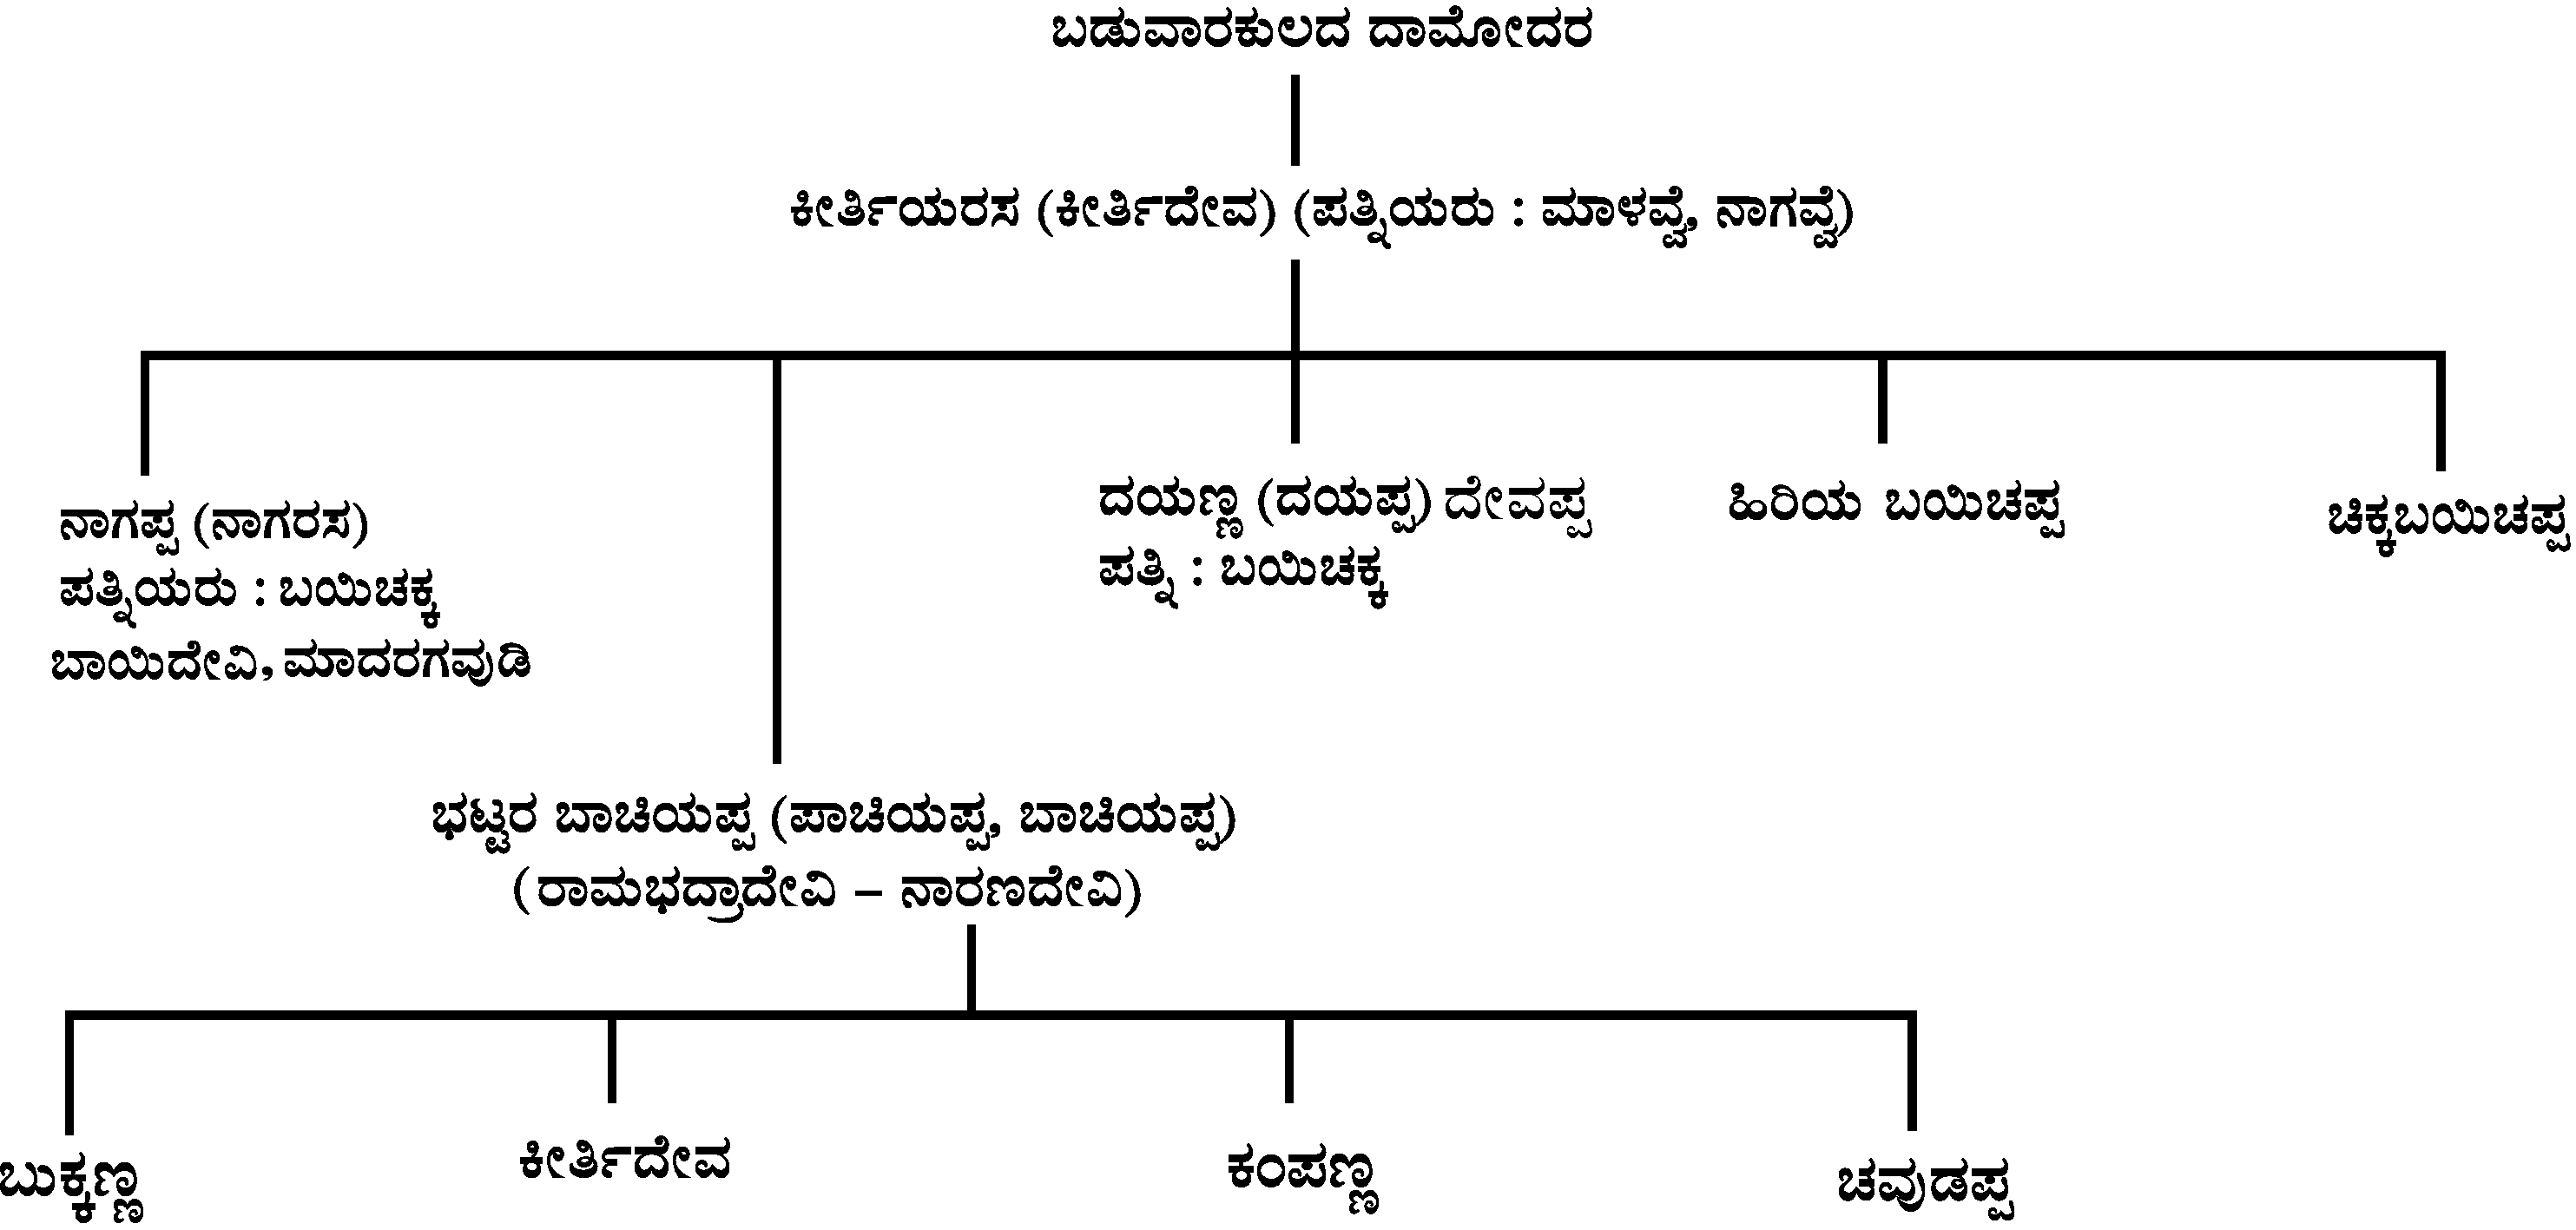
\includegraphics[scale=1.17]{images/chap3/chap3fig37.jpeg}
\end{figure}

\textbf{ಮಹಾಪ್ರಧಾನ ದಂಡನಾಯಕ ಲಖಣ್ಣವೊಡೆಯ (ಲಕ್ಕಣ್ಣ ದಂಡೇಶ)\index{ಲಖಣ್ಣವೊಡೆಯ (ಲಕ್ಕಣ್ಣ ದಂಡೇಶ)} (1402\general{\enginline{-}}1439):} ಲಕ್ಕಣ್ಣ ದಂಡೇಶನು ಪರಮ ಮಾಹೇಶ್ವರನಾಗಿದ್ದು\index{ಪರಮ ಮಾಹೇಶ್ವರ} (ವೀರಶೈವ) ವಿಜಯನಗರ ಒಂದನೇ ದೇವರಾಯನಿಂದ\index{ಒಂದನೇ ದೇವರಾಯ}(1406\enginline{-}1422) ಮೂರನೇ ದೇವರಾಯ\index{ಮೂರನೇ ದೇವರಾಯ} ಅಥವಾ ಮಲ್ಲಿಕಾರ್ಜುನನವರೆಗೆ(1466\enginline{-}1487) ನಾಲ್ಕು ಅರಸರ ಕಾಲದಲ್ಲಿಯೂ, ಅಧಿಕಾರಿಯಾಗಿ, ದಂಡನಾಯಕನಾಗಿ, ಪ್ರಧಾನನಾಗಿ ವಿವಿಧ ಹುದ್ದೆಗಳಲ್ಲಿ, ಸಾಮ್ರಾಜ್ಯದ ವಿವಿಧ ಪ್ರದೇಶಗಳಲ್ಲಿ ಆಡಳಿತವನ್ನು ನಡೆಸುತ್ತಿದ್ದನೆಂಬುದು ತಿಳಿದು ಬರುತ್ತದೆ.\endnote{ ಶಿವಾನಂದ್​ ಡಾ॥ ವಿ., ಪ್ರೌಢದೇವರಾಯನ ಕಾಲದ ಕನ್ನಡ ಸಾಹಿತ್ಯ,, ಪುಟ 36-38.} ಲಕ್ಕಣ್ಣದಂಡೇಶನನ್ನು ಉಲ್ಲೇಖಿಸುವ 21 ಶಾಸನಗಳ ಪಟ್ಟಿಯನ್ನು ಡಾ. ವಿ.ಶಿವಾನಂದ್​\index{ವಿ.ಶಿವಾನಂದ್​} ಅವರು ನೀಡಿದ್ದಾರೆ.\endnote{ ಅದೇ- ಪುಟ 391-393.

ಶೀರೂರ್​, ಡಾ॥ ಬಿ.ವಿ., ಲಕ್ಕಣ್ಣ ದಂಡೇಶ, ಪುಟ 10-11,} ಇವನು ಮಧುರೆ\index{ಮಧುರೆ}, ಮುಳಬಾಗಿಲು\index{ಮುಳಬಾಗಿಲು} ಮತ್ತು ಬಾರಕೂರು\index{ಬಾರಕೂರು} ರಾಜ್ಯಗಳ ಒಡೆಯನಾಗಿದ್ದನೆಂದು ತಿಳಿದುಬರುತ್ತದೆ”.\endnote{ ಶಿವಾನಂದ್​, ಡಾ॥ ವಿ., ಅಮಾತ್ಯ ಶಿರೋಮಣಿ ಲಕ್ಕಣ್ಣದಂಡೇಶ, ಪುಟ 3-5}

\newpage

ಲಕ್ಕಣ್ಣ ದಂಡೇಶನು, ಕ್ರಿ.ಶ.1402ರಿಂದಲೇ ಹೊಯ್ಸಳರಾಜ್ಯದಲ್ಲಿ\index{ಹೊಯ್ಸಳರಾಜ್ಯ}, (ತಲಕಾಡು\index{ತಲಕಾಡು} ನಾಡು) ಅಧಿಕಾರಿಯಾಗಿದ್ದನೆಂಬ ಅಂಶ ಜಿಲ್ಲೆಯ ಶಾಸನಗಳಿಂದ ತಿಳಿದುಬರುತ್ತದೆ. ಎರಡನೇ ಹರಿಹರನ ಕಾಲದಲ್ಲಿ ಲಖಂಣನ ಆದೇಶದಂತೆ ಪುರದ ವೀರಭದ್ರದೇವರಿಗೆ\index{ಪುರದ ವೀರಭದ್ರದೇವರು} ಅನೇಕ ತೆರಿಗೆಗಳನ್ನು ಬಿಡಲಾಗಿದೆ.\endnote{ ಎಕ 6 ಪಾಂಪು 260, 261 ಪುರ 1402} 1403ರ ಬಲಮುರಿ ಶಾಸನದಲ್ಲಿ ಲಖಂಣವೊಡೆಯರ ನಿರೂಪದಿಂದ, ಬೆಳಗೊಳದ\index{ಬೆಳಗೊಳ} ಅಳಗುವಂಣನು\index{ಅಳಗುವಂಣ}, ಅಗಸ್ತ್ಯೇಶ್ವರ\index{ಅಗಸ್ತ್ಯೇಶ್ವರ} ದೇವಾಲಯವನ್ನು ಜೀರ್ಣೋದ್ಧಾರ ಮಾಡುತ್ತಾನೆ. ಈ ಶಾಸನದಲ್ಲಿ ಲಕ್ಕಣ್ಣನನ್ನು ಒಡೆಯನೆಂದು ಹೇಳಿದೆ.\endnote{ ಎಕ 6 ಶ‍್ರೀಪ 77 ಬಲಮುರಿ 1403} ಪ್ರೌಢದೇವರಾಯನ ಕಾಲಕ್ಕೆ ಇವನು ಮಹಾಪ್ರಧಾನ ಹುದ್ದೆಗೇರಿದ್ದು ಕ್ರಿ.ಶ.1439ರ ಮಳವಳ್ಳಿ ತಾ. ಕ್ಯಾತನಹಳ್ಳಿ\index{ಕ್ಯಾತನಹಳ್ಳಿ} ಶಾಸನದಿಂದ ತಿಳಿದುಬರುತ್ತದೆ. ಮಹಾಪ್ರಧಾನ ಲಕ್ಕಣ್ಣ ದಂಣಾಯಕರ ನಿರೂಪದಿಂದ ತಳಕಾಡು ಪಟ್ಟಣದ\index{ತಲಕಾಡು ಪಟ್ಟಣ} ಅಧಿಕಾರಿ ರಾಯಂಣ ಒಡೆಯ ಮತ್ತು ತಳಕಾಡ ನಾಡ\index{ತಳಕಾಡ ನಾಡು} ಅಥವಾ ಮಾಗಣಿಯ\index{ಮಾಗಣಿ} ಅಧಿಕಾರಿ ಪೆರಮಾಳು ದೇವರಸ\index{ಪೆರಮಾಳು ದೇವರಸ} ಇವರು, ತಳಕಾಡು ಕೀರ್ತಿನಾರಾಯಣದೇವರ, ಪವಿತ್ರಾರೋಹಣ, ಶ‍್ರೀಕಾರ್ಯಕ್ಕೆ ಕೇತನಹಳ್ಳಿ ಮತ್ತು ರಠಹಳ್ಳಿಯ ಸುಂಕಗಳನ್ನು ದತ್ತಿಯಾಗಿ ಬಿಡುತ್ತಾರೆ.\endnote{ ಎಕ 7 ಮವ 133 ಮತ್ತು 134 ಕ್ಯಾತನಹಳ್ಳಿ 1439} ಕಾವೇರಿ ನದಿ\index{ಕಾವೇರಿ (ನದಿ-ಹೊಳೆ)} ಪಶ್ಚಿಮವಾಹಿನಿ\index{ಪಶ್ಚಿಮವಾಹಿನಿ} ತೀರದ, ಗಜಾರಣ್ಯ\index{ಗಜಾರಣ್ಯ} ಕ್ಷೇತ್ರವಾದ ತಲಕಾಡ ವೈದ್ಯನಾಥ ದೇವರಿಗೆ\index{ತಲಕಾಡ ವೈದ್ಯನಾಥ ದೇವರು} ನಡೆಯುತ್ತಿದ್ದ ಕಟ್ಟಳೆಯ ಧರ್ಮವು ಸರಿಯಾಗಿ ನೆರವೇರದೇ ಇರಲು, ಇಮ್ಮಡಿ ದೇವರಾಯನಿಗೆ\index{ಇಮ್ಮಡಿ ದೇವರಾಯ} ಸಕಲ ಆಯುರಾರೋಗ್ಯ ಐಶ್ವರ್ಯ ಅಭಿವೃದ್ಧಿ ಆಗಬೇಕೆಂದು, ಲಕ್ಕಣ್ಣ ದಂಡನಾಯಕನು ತಳಕಾಡು ವೈದ್ಯನಾಥದೇವರಿಗೆ ಬೆಳಕವಾಡಿ ಠಾಣೆಯ ಸ್ಥಾವರ ಸುಂಕಗಳನ್ನು ದತ್ತಿ ಬಿಡುತ್ತಾನೆ. ಈ ಬಗ್ಗೆ ದಂಣಾಯಕ ಒಡೆಯರ ಅಂದರೆ ಲಕ್ಕಣ್ಣದಂಡನಾಯಕರ ರಾಯಸವು\index{ರಾಯಸ} ತಳಕಾಡ ಪಟ್ಟಣದ ಅಧಿಕಾರಿ ರಾಯಣ್ಣ ಒಡೆಯನಿಗೆ\index{ರಾಯಣ್ಣ ಒಡೆಯ} ಬಂದಿತೆಂದೂ, ಆ ರಾಯಣ್ಣ ಒಡೆಯನ ನಿರೂಪದಿಂದ ತಳಕಾಡ ಪೆರುಮಾಳದೇವನು ಕಿರಗಸೂರು ಗ್ರಾಮದ ಸುಂಕಗಳನ್ನೂ ಕೂಡಾ ವೈದ್ಯನಾಥದೇವರಿಗೆ ಸರ್ವಮಾನ್ಯವಾಗಿ ದತ್ತಿ ಬಿಟ್ಟನೆಂದೂ ಹೇಳಿದೆ.\endnote{ ಎಕ 7 ಮವ 102 ಕಿರಗಸೂರು 1440 ಆಗಸ್ಟ್​ 8} ಇಮ್ಮಡಿ ದೇವರಾಯನ ಆಳ್ವಿಕೆಯ ಕೊನೆಗಾಲದಲ್ಲಿ (1442\enginline{-}43ರ ಸುಮಾರಿನಲ್ಲಿ) ಅವನನ್ನು ಕೊಲ್ಲುವ ಪ್ರಯತ್ನವು ನಡೆಯಿತೆಂದು ಈ ಗಂಡಾಂತರದಿಂದ ರಾಯನು ಪಾರಾದನೆಂದು ತಿಳಿದುಬರುತ್ತದ.\endnote{ ದೇಸಾಯಿ, ಡಾ॥ ಪಿ.ಬಿ., ವಿಜಯನಗರ ಸಾಮ್ರಾಜ್ಯ, ಪುಟ 45

ಸೂರ್ಯನಾಥ ಕಾಮತ್​, ಡಾ॥, ಕರ್ನಾಟಕದ ಸಂಕ್ಷಿಪ್ತ ಇತಿಹಾಸ, ಪುಟ 127} ರಾಯನಿಗೆ ಆಯುರಾರೋಗ್ಯ ಐಶ್ವರ್ಯ ಅಭಿವೃದ್ಧಿಯಾಗಬೇಕೆಂದು ವೈದ್ಯನಾಥನಿಗೆ 1440ರಲ್ಲಿ ದತ್ತಿ ಬಿಟ್ಟಿರುವುದನ್ನು ನೋಡಿದರೆ ಈ ಘಟನೆ 1440ರಲ್ಲೇ ನಡೆದಿದೆ ಎಂದು ಊಹಿಸಬಹುದು.

ಲಕ್ಕಣ್ಣ ದಂಡನಾಯಕ ಮತ್ತು ಮಾದಣ್ಣ ದಂಡನಾಯಕರು\index{ಮಾದಣ್ಣ ದಂಡನಾಯಕ}, ವಿಷ್ಣುವರ್ಧನ ಗೋತ್ರದ\index{ವಿಷ್ಣುವರ್ಧನ ಗೋತ್ರ} ಹೆಗ್ಗಡೆದೇವ\index{ಹೆಗ್ಗಡೆದೇವ} ಮತ್ತು ವೊಮ್ಮಯ್ಯಮ್ಮ (ವೊಮ್ಮಾಯಮ್ಮ)\index{ವೊಮ್ಮಯ್ಯಮ್ಮ (ವೊಮ್ಮಾಯಮ್ಮ)} ಇವರ ಮಕ್ಕಳೆಂದು, ಇವರು ಮುಳಬಾಗಿಲು\index{ಮುಳಬಾಗಿಲು} ಮತ್ತು ವಿರೂಪಾಕ್ಷಿಪುರಗಳಲ್ಲಿ\index{ವಿರೂಪಾಕ್ಷಿಪುರ} ದೇವಾಲಯಗಳು, ಮಂಟಪಗಳು, ಮಠಗಳು, ಮನ್ಮಥಪುಷ್ಕರಣಿಗಳನ್ನು ನಿರ್ಮಿಸಿ, ದತ್ತಿ ಹಾಕಿ ಕೊಟ್ಟರೆಂದು ತಿಳಿದು ಬರುತ್ತದೆ.\endnote{ ಇಸಿ 10 ಮುಳಬಾಗಿಲು 2 ಮುಳಬಾಗಿಲು 1431, ಮುಳಬಾಗಿಲು 96 ವಿರೂಪಾಕ್ಷಿಪುರ 1431}

\textbf{ಮಹಾಪ್ರಧಾನ ಹೆಗ್ಗಪ್ಪ\index{ಮಹಾಪ್ರಧಾನ ಹೆಗ್ಗಪ್ಪ} (1406):} ವೀರಪ್ರತಾಪ ಹರಿಹರ ಮಹಾರಾಯನ ಅರಮನೆಯ ಮಹಾಪ್ರಧಾನರಾದ, ಆತ್ರೇಯ ಗೋತ್ರದ ಹೆಗ್ಗಪ್ಪಗಳು, ಮಾರೇಹಳ್ಳಿ ಲಕ್ಷ್ಮೀನರಸಿಂಹ ದೇವಾಲಯದ\index{ಮಾರೇಹಳ್ಳಿ ಲಕ್ಷ್ಮೀನರಸಿಂಹ ದೇವಾಲಯ} ಗೋಪುರಗಳಿಗೆ ಹೊನ್ನ ಕಳಸಗಳನ್ನು\index{ಹೊನ್ನ ಕಳಸ} ಮಾಡಿಸಿಕೊಟ್ಟಂತೆ ಹೇಳಿದೆ. ಇವನ ಜೊತೆಯಲ್ಲಿ ಮಲ್ಲರಸನೂ\index{ಮಲ್ಲರಸ} ಕೂಡಾ ಹೊನ್ನ ಕಳಸವನ್ನು ಮಾಡಿಸಿಕೊಟ್ಟಿದ್ದಾನೆ.\endnote{ ಎಕ 7 ಮವ 71 ಮಾರೇಹಳ್ಳಿ 1406}

\textbf{ಮಹಾಪ್ರಧಾನ ಪುಲಿಯಣ್ಣ ಒಡೆಯ\index{ಮಹಾಪ್ರಧಾನ ಪುಲಿಯಣ್ಣ ಒಡೆಯ} (1420):} ಒಂದನೆಯ ಪ್ರತಾಪದೇವರಾಯನ ಕಾಲದಲ್ಲಿ ಮಹಾಪ್ರಧಾನ\-ನಾಗಿದ್ದ ಪುಲಿಯಣ್ಣ ಒಡೆಯನ ನಿರೂಪದಂತೆ, ವಿಶೇಷದ (ಅಧಿಕಾರಿ) ದೇವರಸ\index{ವಿಶೇಷದ (ಅಧಿಕಾರಿ) ದೇವರಸ} ಒಡೆಯನು ಬೆಳಕವಾಡಿಯ ಸ್ವಯಂಭು ವೈಜನಾಥದೇವರ\index{ಬೆಳಕವಾಡಿಯ ಸ್ವಯಂಭು ವೈಜನಾಥದೇವರು} ನಂದಾದೀವಿಗೆಗೆ ದತ್ತಿ ಬಿಡುತ್ತಾನೆ.\endnote{ ಎಕ 7 ಮವ 96 ಬೆಳಕವಾಡಿ 1420}

\textbf{ಮಹಾಪ್ರಧಾನ ಚಿಕವಡೆಯ\index{ಮಹಾಪ್ರಧಾನ ಚಿಕಒಡೆಯ} (1424):} ಶ‍್ರೀಮನ್​ ಮಹಾಪ್ರಧಾನ ಸಿ....ರಿ ಒಡೆಯ ಮತ್ತು ಚಾಮಾಂಬಿಕೆಗೆ ಜನಿಸಿದ ಶ‍್ರೀಮನ್​ ಮಹಾಪ್ರಧಾನ ಚಿಕವಡೆಯರು, ಭಯಿರಮೇಶ್ವರಪುರ ಅಗ್ರಹಾರದಲ್ಲಿ\index{ಭಯಿರಮೇಶ್ವರಪುರ ಅಗ್ರಹಾರ} ಮಹಾಜನಗಳಿಂದ ಗದ್ದೆಯನ್ನು ಕ್ರಯವಾಗಿ ಕೊಂಡು ಅದನ್ನು ಸೋಮನಾಥದೇವರ ವೃತ್ತಿಯಾಗಿ\index{ಸೋಮನಾಥದೇವರ ವೃತ್ತಿ} ಧಾರೆಯೆರೆದು, ಬ್ರಾಹ್ಮಣರ ಭೋಜನಕ್ಕೆ ದತ್ತಿ ಬಿಡುತ್ತಾರೆ.\endnote{ ಎಕ 6 ಕೃಪೇ 96 ಭೈರಾಪುರ 1424} ಬುಕ್ಕಣ್ಣ ಒಡೆಯರು\index{ಬುಕ್ಕಣ್ಣ (ಬುಕ್ಕರಾಯ ಒಡೆಯ - ನೃಪತಿ - ಮಹೀಪಾಲ)} ಮತ್ತು ಮಲ್ಲಾಂಬಿಕೆಗೆ\index{ಮಲ್ಲಾಂಬಿಕೆ} ಜನಿಸಿದ ಮಗನ ಹೆಸರು ಈ ಶಾಸನದಲ್ಲಿ ತ್ರುಟಿತವಾಗಿದೆ. ಎರಡನೆಯ ಬುಕ್ಕರಾಯನಿಗೆ ಮಲ್ಲಾದೇವಿಯಿಂದ ಒಂದನೆಯ ವಿರೂಪಾಕ್ಷನೆಂಬ\index{ಒಂದನೆಯ ವಿರೂಪಾಕ್ಷ} ಮಗನಿದ್ದನು. ಆದರೆ ಅವನ ಕಾಲ ಕ್ರಿ.ಶ.1384\enginline{-}1404 ಎಂದು ರೈಸ್​ ಹೇಳಿದ್ದಾರೆ.\endnote{ \engfoot{Rice, B.L., Mysore and Coorg from the Inscriptions, pp.112}}

\textbf{ಮಹಾಪ್ರಧಾನ ದಂಡನಾಯಕ ತಿಮ್ಮಣ್ಣ\index{ಮಹಾಪ್ರಧಾನ ದಂಡನಾಯಕ ತಿಮ್ಮಣ್ಣ} (1458):} ಲೋಹಿತ ವಂಶದ\index{ಲೋಹಿತ ವಂಶ} ಮಹಾಪ್ರಧಾನ ತಿಮ್ಮಣ್ಣ ದಂಡನಾಯಕನು\index{ತಿಮ್ಮಣ್ಣ ದಂಡನಾಯಕ (ದಂಡನಾಥ)}, ನಾಗಮಂಗಲದ ಮಹಾ ಪ್ರಭುವಾಗಿದ್ದ\index{ನಾಗಮಂಗಲದ ಮಹಾ ಪ್ರಭು}, ಶಿಂಗಣ್ಣ ಒಡೆಯನ\index{ಶಿಂಗಣ್ಣ ಒಡೆಯ} ಮಗ. ತಿಮ್ಮಣ್ಣನು, ಮಲ್ಲಿಕಾರ್ಜುನ\index{ಮಲ್ಲಿಕಾರ್ಜುನ} ಮತ್ತು ಮೂರನೆಯ ವಿರೂಪಾಕ್ಷ\index{ಮೂರನೆಯ ವಿರೂಪಾಕ್ಷ} ಇವರ ಕಾಲದಲ್ಲಿ (1446 ರಿಂದ 1485ರವರೆಗೆ) ಮಹಾಪ್ರಧಾನ ದಂಡನಾಯಕನಾಗಿದ್ದಂತೆ ತೋರುತ್ತದೆ.

\textbf{“ಶುದ್ಧ ಲೋಹಿತ ವಂಶ\index{ಶುದ್ಧ ಲೋಹಿತ ವಂಶ} ಮೌಕ್ತಿಕ ಸಿಂಗಣಾಖ್ಯ ಮಹಾಪ್ರಭೋತ್ತಮೂರ್ತಿರನೇಕ ಜನ್ಮತಪಃ ಫಲಾತಿಶಯಃ ಕ್ಷಾಮಿಸ್ಫುರನ್​ ಧೀರ ತಿಂಮಣ ದಂಡನಾಥೋ ಸ್ತೀರೋಮಣಿ ಸ್ಥಿರವೈಭವಸ್ತಸ್ಯ ರಾಜ್ಯ ದುರಂಧರೋ ಧರಣೀತೇಃ ಸಚಿವೋಭವತ್​”} ಎಂದು ನೆಲಮನೆ ಶಾಸನವು ತಿಮ್ಮಣ್ಣನ್ನು ವರ್ಣಿಸಿದೆ.\endnote{ ಎಕ 6 ಶ‍್ರೀಪ 93 ನೆಲಮನೆ 1458}\textbf{“ನಾಗಮಂಗಲದ ಮಹಾಪ್ರಭು ಪರಮಭಾಗವತ ಲೋಹಿತಕುಲಶೇಖರ ಶಿಂಗಂಣಗಳ\index{ಲೋಹಿತಕುಲಶೇಖರ ಶಿಂಗಂಣ} ಮಖ್ಖಳು ಸೀತಾಂಬಿಕಾ\index{ಸೀತಾ ಅಮ್ಮನವರು (ಸೀತಾಂಬಿಕಾ)} ತಪಃಫಲ ವೇದಮಾರ್ಗ ಪ್ರತಿಷ್ಠಾಚಾರ್ಯ ಯಾದವಗಿರಿ ಜೀರ್ಣೋದ್ಧಾರಕ\index{ಯಾದವಗಿರಿ ಜೀರ್ಣೋದ್ಧಾರ} ಯದುಗಿರಿ ನಾರಾಯಣ ಚರಣಾರವಿಂದ ಭಕ್ತಿ ತತ್ರಯಿಕ ನಿಷ್ಟ ತುಲಾಪುರಷಾದಿ ಮಹಾದಾನ ದೀಕ್ಷಿತ ರಂಗಾಂಬಿಕಾ\index{ರಂಗಮಾಂಬ(ಬೆ), ರಂಗಮಾಂಬಿಕೆ, ರಂಗಾಂಬಿಕಾ(ಕೆ)} ಮನೋವಲ್ಲಭ ಶ‍್ರೀಮಂನ್​ ಮಹಾಪ್ರಧಾನ ತಿಂಮಂಣ್ನ ದಂಣ್ನಾಯಕರು”} ಎಂದು ಮೇಲುಕೋಟೆಯ ಶಾಸನ ವರ್ಣಿಸಿದೆ.\endnote{ ಎಕ 6 ಪಾಂಪು 179 ಮೇಲುಕೋಟೆ 1458}\textbf{ “ಶ‍್ರೀನಾರಾಯಣ\-ದೇವರ ಚರಣಾರವಿಂದ ಭರತ ತತ್ವೈಕನಿಷ್ಠುರ ತುಲಾಪುರುಷಾದಿ ಮಹಾದಾನ ವ್ರತದೀಕ್ಷಿತ ಅಭಿನವಕುಲಶೇಖರರಾದ\index{ಅಭಿನವಕುಲಶೇಖರ} ಶ‍್ರೀಮನ್​ ಮಹಾಪ್ರಧಾನ ತಿಮ್ಮಣ್ಣ ದಂಣಾಯಕ ಒಡೆಯರು” ಎಂದು ಮೇಲುಕೋಟೆಯ ಇನ್ನೊಂದು ಶಾಸನವು ಇವನನ್ನು ವರ್ಣಿಸಿದೆ.\endnote{ ಎಕ 6 ಪಾಂಪು 163 ಮೇಲುಕೋಟೆ 1469}}

ತಿಮ್ಮಣ್ಣ ದಂಡನಾಯಕ\index{ತಿಮ್ಮಣ್ಣ ದಂಡನಾಯಕ (ದಂಡನಾಥ)} ಮತ್ತು ಅವನ ಪತ್ನಿ ಪರಮ ಭಾಗವತೋತ್ತಮೆ ರಂಗಮ್ಮನವರು\index{ರಂಗಮ್ಮ}, ನಾರಾಯಣ ಪ್ರೀತ್ಯರ್ಥವಾಗಿ ಮೇಲುಕೋಟೆಯಲ್ಲಿ\index{ಮೇಲುಕೋಟೆ} ರತ್ನಾಭರಣ\index{ರತ್ನಾಭರಣ} ರಜತಪರಿಯಂಕ ಮಂಟಪ\index{ರಜತಪರಿಯಂಕ ಮಂಟಪ}, ಮಹಾತಟಾಕಾದಿ\index{ಮಹಾತಟಾಕ} ಸಕಲ ವಿಧ ಕೈಂಕರ್ಯಗಳನ್ನು ಮಾಡಿ, ದೇಶಾಂತರ ಮಠವನ್ನು\index{ದೇಶಾಂತರ ಮಠ} ಕಟ್ಟಿಸಿ, ವೈಷ್ಣವರ ಭೋಜನಕ್ಕೆ ಮೇಲುಕೋಟೆಯ ಕಾಲುವಳ್ಳಿಗಳಾದ ಬಲ್ಲೇನಹಳ್ಳಿ\index{ಬಲ್ಲೇನಹಳ್ಳಿ} ಮತ್ತು ಯಲವದ ಹಳ್ಳಿಗಳನ್ನು\index{ಯಲವದ ಹಳ್ಳಿ (ಪಲ್ಲಿ)} ದತ್ತಿಯಾಗಿ ಬಿಡುತ್ತಾರ.\endnote{ ಎಕ 6 ಪಾಂಪು 179 ಮೇಲುಕೋಟೆ 1458} ಮೇಲುಕೋಟೆಯಲ್ಲಿ ಶ‍್ರೀರಂಗಮಂಟಪವನ್ನು ನಿರ್ಮಿಸಿ, ಬ್ರಾಹ್ಮಣರ ಭೋಜನಕ್ಕೆ ಮತ್ತು ಮಹಾಲಕ್ಷ್ಮಿಯ ಸೇವೆಗೆ ಇಮ್ಮಡಿ ಪ್ರೌಢದೇವರಾಯನ (ವಿರೂಪಾಕ್ಷ) ಅನುಮತಿಯಿಂದ ಬಲ್ಲೇನಹಳ್ಳಿ ಮತ್ತು ಯಲವದಹಳ್ಳಿಗಳನ್ನು ಅಗ್ರಹಾರದ್ವಯವನ್ನಾಗಿ\index{ಅಗ್ರಹಾರದ್ವಯ} ಮಾಡಿದರೆಂದು ನೆಲಮನೆ\index{ನೆಲಮನೆ} ಶಾಸನದಿಂದ ತಿಳಿದುಬರುತ್ತದೆ.\endnote{ ಎಕ 6 ಶ‍್ರೀಪ 93 ನೆಲಮನೆ 1458} ತಿಮ್ಮಣ್ಣ ದಂಡನಾಯಕನು ತಿರುನಾರಾಯಣಪುರಕ್ಕೆ ಸೇರಿದ, ತನ್ನ ನಾಯಕತನಕ್ಕೆ ಸಲ್ಲುವ ಹೊಸಹಳ್ಳಿಯನ್ನು ತಮ್ಮ ತಾಯಿ ಸೀತಾಯಂಮ\-ನವರ\index{ಸೀತಾ ಅಮ್ಮನವರು (ಸೀತಾಂಬಿಕಾ)} ಧರ್ಮಾಗ್ರಹಾರವಾಗಿ ಮಾಡಿ 20 ಮಹಾಜನಗಳಿಗೆ ದತ್ತಿಹಾಕಿಕೊಡುತ್ತಾನೆ.\endnote{ ಎಕ 6 ಪಾಂಪು 153 ಮೇಲುಕೋಟೆ 1460}

ಮಹಾಪ್ರಧಾನ ತಿಮ್ಮಣ್ಣ ದಂಡನಾಯಕನು, ತನ್ನ ಅರಸ ಮಲ್ಲಿಕಾರ್ಜುನನ ಜೊತೆ ಸಾಳುವ ನರಸಿಂಗನ \textbf{“ರಾಜಕಾರ್ಯ\-ಕ್ಕಾಗಿ ಪೆನುಗೊಂಡೆಯೊಳು ಸುಕದಿಂ ರಾಜ್ಯವನಾಳುತ್ತಮಿದ್ದ”} ಸಂದರ್ಭದಲ್ಲಿ \textbf{“ದಂಡನಾಯಕನು ಸೀಮೆಯಿಂ ಬಪ್ಪಡೆ”} ಮಳಲಿಯ ತಿಪ್ಪಯ್ಯನು, ಅವರ ಚಿತ್ತಮಂ ಪಡೆದು ಬೆಳತೂರ ರಾಮಯ್ಯ ದೇವರಿಗೆ ದತ್ತಿ ಬಿಟ್ಟನೆಂದು ತಿಳಿದುಬರುತ್ತದೆ.\endnote{ ಎಕ 7 ಮಂ 39 ದಣ್ಣಾಯಕನಪುರ 1459, ಎಕ 7 ಮ 24 ರಾಂಪುರ 1459} ಬಹುಶಃ ತಿಮ್ಮಣ್ಣ ದಂಡನಾಯಕನು ಈ ಸಂದರ್ಭದಲ್ಲಿ ಮೇಲುಕೋಟೆ\index{ಮೇಲುಕೋಟೆ} ಮತ್ತು ನಾಗಮಂಗಲದ ಕಡೆಗೆ ಬಂದಿರಬಹುದು. ತಿಮ್ಮಣ್ಣ ದಂಡನಾಯಕನು ಈ ಕಾಲದಲ್ಲಿ ದುರ್ಬಲವಾಗಿದ್ದ ವಿಜಯನಗರ ಸಾಮ್ರಾಜ್ಯವನ್ನು ಉಳಿಸಲು ಸಾಳುವ ನರಸಿಂಗನ ಜೊತೆ ಸೇರಿ ಕೆಲಸ ಮಾಡಿರಬಹುದು. ತಿಮ್ಮಣ್ಣ ದಂಡನಾಯಕನ ತಮ್ಮನಾದ ದೇವರಾಜನು ಹರಹಿನ ಸೀಮೆಯಲ್ಲಿ\index{ಹರಹಿನ ಸೀಮೆ} ಕಾಲುವೆಯನ್ನು ನಿರ್ಮಿಸಿ, ಹೊಸಹಳ್ಳಿ ಗ್ರಾಮವನ್ನು ತನ್ನ ತಾಯಿ ಸೀತಾಯಂಮವನರ ಹೆಸರಿನಲ್ಲಿ ಸೀತಾಪುರವೆಂಬ\index{ಸೀತಾಪುರ ಅಗ್ರಹಾರ} ಅಗ್ರಹಾರವನ್ನಾಗಿ ಮಾಡುತ್ತಾನೆ. ಆದರೆ ಈ ಶಾಸನದಲ್ಲಿ ತಿಮ್ಮಣ್ಣ ದಂಡನಾಯಕನ ಹೆಸರಿಲ್ಲ.\endnote{ ಎಕ 6 ಪಾಂಪು 19 ಸೀತಾಪುರ 1467} ತಿಮ್ಮಣ್ಣ ದಂಡನಾಯಕನೂ ಈ ಕಾರ್ಯದಲ್ಲಿ ಜೊತೆಯಾಗಿ ಸೇರಿರಬಹುದೆಂದು ಮೇಲೆ ಉಲ್ಲೇಖಿಸಿದ, ಮೇಲುಕೋಟೆ ಶಾಸನದಿಂದ ಊಹಿಸಬಹುದು.

ದೇವರಾಜ ಒಡೆಯನು ಇಮ್ಮಡಿ ದೇವರಾಯನ ನಿರೂಪದಂತೆ ಸಂಪತ್ಕರ ನಾರಾಯಣದೇವರ ವಸಂತೋತ್ಸವ\index{ವಸಂತೋತ್ಸವ} ತಿರುನಾಳಿಗೆ, ಅಮೃತಪಡಿಗೆ, ನಂದಾದೀವಿಗೆಗೆ, ವನಮಾಲೆಗೆ ತನ್ನ ಧರ್ಮವಾಗಿ, ಹೊಸಹಳ್ಳಿ ಗ್ರಾಮದ ಹಿರಿಯಕೆರೆಯಕೆಳಗೆ ಮತ್ತು ಮಯಿಲನಹಳ್ಳಿಯಲ್ಲಿ ಗದ್ದೆಗಳನ್ನು, 505 ಪಣವನ್ನು ದತ್ತಿಯಾಗಿ ಬಿಡುತ್ತಾನೆ.\endnote{ ಎಕ 6 ಪಾಂಪು 152 ಮೇಲುಕೋಟೆ 1432} ಶ‍್ರೀರಂಗಪಟ್ಟಣದ\index{ಶ‍್ರೀರಂಗಪಟ್ಟಣ} ಸೌಮ್ಯರಾಜ ರಂಗನಾಥನಿಗೆ\index{ಸೌಮ್ಯರಾಜ ಶ‍್ರೀರಂಗನಾಥ} ಶ‍್ರೀರಂಗಪುರದ ಮಹಾಜನಗಳಿಂದ ಕೆಲವು ಸುಂಕಗಳನ್ನು ದತ್ತಿಯಾಗಿ ಬಿಡಿಸುತ್ತಾನೆ.\endnote{ ಎಕ 6 ಶ‍್ರೀಪ 3 ಶ‍್ರೀರಂಗಪಟ್ಟಣ 1431}

ಗೊರಊರು (ಗೊರೂರು) ಗ್ರಾಮವು ಜೀರ್ಣವಾಗಿದ್ದಾಗ ಅಲ್ಲಿಯ ಅಶೇಷ ಮಹಾಜನಗಳು ತಿಮ್ಮಣ್ಣ ದಂಡನಾಯಕ\-ನಿಗೆ ಬಿನ್ನಹಮಾಡಿ ಅರಮನೆಯಿಂದ 125 ಗದ್ಯಾಣ ಧನಸಹಾಯವನ್ನು ಪಡೆದು, ಅದನ್ನು ತಳವಾರ ನರಸಿಂಗಣ್ಣಗಳಿಗೆ ಕೊಟ್ಟರೆಂದು, ಹೊಸ ದೇವಾಲಯವನ್ನು ನಿರ್ಮಿಸಿ ಹಳೆಯ ವಾಸುದೇವ ಮೂರ್ತಿಯನ್ನು ಅಲ್ಲಿಡಲಾಯಿತೆಂದು ತಿಳಿದು\-ಬರುತ್ತದೆ.\endnote{ ಎಕ 8 ಹಾಸನ 201 ಗೊರೂರು 1466} ಮಲ್ಲಿಕಾರ್ಜುನ ಮಹಾರಾಯರು ಪ್ರಧಾನ ತಿಮ್ಮಣ್ಣ ದಂಡನಾಯಕನಿಗೆ ನಿರೂಪವನ್ನು ನೀಡಿ, ತಮ್ಮ ರಾಜಧನತ್ವಕ್ಕೆ ಸಲ್ಲುವ ಸ್ವಾತಿ ಗ್ರಾಮ (ಶಾಂತಿಗ್ರಾಮ) ಸೀಮೆಯ ಲಕ್ಷ್ಮೀಸಾಗರವನ್ನು\index{ಲಕ್ಷ್ಮೀಸಾಗರ} ಮಲ್ಲರಾಜನ ಮಗ ಭಟ್ಟರ ನುಕರಾಜನಿಗೆ ದತ್ತಿ ಕೊಡಿಸಿದರೆಂದು ಹೇಳಿದೆ.\endnote{ ಎಕ 8 ಹಾಸನ 125 ಲಕ್ಷ್ಮೀಸಾಗರ 1458-59}

\newpage

ಇವನ ವಂಶವೃಕ್ಷವನ್ನು ಈ ಕೆಳಗಿನಂತೆ ಕಟ್ಟಿಕೊಡಬಹುದು,

\begin{figure}[H]
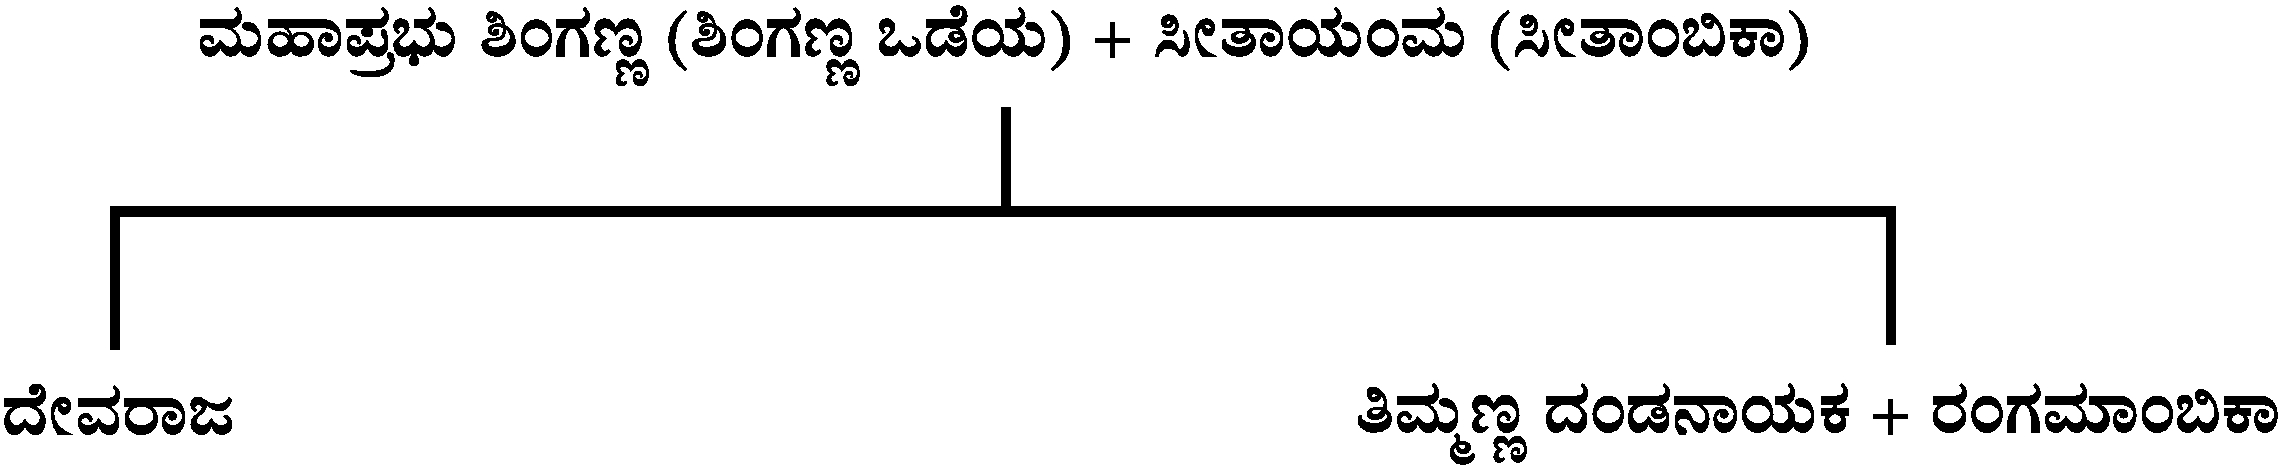
\includegraphics[scale=1.2]{images/chap3/chap3fig38.jpeg}
\end{figure}

\vskip -3pt

\textbf{ಮಹಾಪ್ರಧಾನ ವಿರೂಪಾಕ್ಷದೇವ ಅಂಣ\index{ಮಹಾಪ್ರಧಾನ ವಿರೂಪಾಕ್ಷದೇವ ಅಂಣ} (1484):} ವಿರೂಪಾಕ್ಷ ದೇವ ಅಣ್ಣನು, ಮಹಾಮಂಡಳೇಶ್ವರ ಕಠಾರಿ ಸಾಳುವ ನರಸಿಂಗ ರಾಜವೊಡೆಯನ ಮನೆಯ (ಅರಮನೆಯ) ಪ್ರಧಾನನಾಗಿರುತ್ತಾನೆ. ಈತನು ಆರಣಿಯ ಸ್ಥಳದ\index{ಆರಣಿಯ ಸ್ಥಳ} ಚುಂಚನಹಳ್ಳಿಯನ್ನು ತನ್ನ ಹೆಸರಿನಲ್ಲಿ ವಿರೂಪಾಕ್ಷಪುರವೆಂದು\index{ವಿರೂಪಾಕ್ಷಪುರ} ನಾಮಕರಣ ಮಾಡಿ ಚುಂಚನ ಭಯಿರಮೇಶ್ವರ ದೇವರಿಗೆ ಸರ್ವಮಾನ್ಯವಾಗಿ ದತ್ತಿ ಬಿಡುತ್ತಾನೆ.\endnote{ ಎಕ 7 ನಾಮಂ 108 ಚುಂಚನಹಳ್ಳಿ 1484} ಈ ವೇಳೆಗೆ ಚುಂಚನಗಿರಿಯು ಭೈರವೇಶ್ವರ ಕ್ಷೇತ್ರವಾಗಿ ಪ್ರಸಿದ್ಧಿಯನ್ನು ಹೊಂದಿತ್ತು.

\vskip -1pt

\textbf{ಮಹಾಪ್ರಧಾನ ಕಾಮೆಯನಾಯಕ\index{ಮಹಾಪ್ರಧಾನ ಕಾಮೆಯ ದಂಡನಾಯಕ} (1512):} ಶ‍್ರೀಮನ್​ ಮಹಾಪ್ರಧಾನ ಕಾಮೆಯನಾಯಕರ ಸೇನಬೋವ ರಾಮಣ್ಣನು, ಮಲಯಾಳನ ಅರಕೆರೆ ಅಗ್ರಹಾರದ ಅಧಿಕಾರಿಯಾಗಿರುತ್ತಾನೆ. ಈತನು ಬಹುಶಃ ಕಾಮೆಯನಾಯಕನ ಅಪ್ಪಣೆಯ ಮೇರೆಗೆ, ಅರಕೆರೆಯ ನರಸಿಂಹದೇವರ ಅಮೃತಪಡಿಗೆ ಗದ್ದೆಯನ್ನು ಕ್ರಯವಾಗಿ ಅಕರವಾಗಿ ಕೊಂಡು ದತ್ತಿ ಬಿಡುತ್ತಾನೆ.\endnote{ ಎಕ 6 ಶ‍್ರೀಪ 110 ಅರಕೆರೆ 1512} ಮಹಾಪ್ರಧಾನ ಕಾಮೆಯನಾಯಕನು ಮುಮ್ಮಡಿ ಬಲ್ಲಾಳನ ಕಾಲದಲ್ಲಿದ್ದ ಕಾಮೆಯ ದಂಡನಾಯಕ ವಂಶದವನಾಗಿರಬಹುದು.

\vskip -1pt

\textbf{ಮಹಾಪ್ರಧಾನ ಚಿಕ್ಕ..ರಾಜ (1591):} ಎರಡನೇ ವೆಂಕಟಪತಿ ದೇವರಾಯನ (1586\enginline{-}91) ಮಹಾಪ್ರಧಾನ ಚಿಕ್ಕ...ರಾಜ ಅರಸುಗಳ ಕಾರ್ಯಕರ್ತನಾದ ಅಧಿಕಾರಿಯು, ರಾಮರಾಜಯ್ಯನಿಗೆ ಪುಣ್ಯವಾಗಬೇಕೆಂದು ಮದ್ದೂರ ನಾರಸಿಂಹ ದೇವರು, ರಾಮಚಂದ್ರ ದೇವರು, ಅಲ್ಲಾಳನಾಥ ದೇವರಿಗೆ ಶಿವಪುರದೊಳಗಣ ಕುಪ್ಪೆಮದ್ದೂರನ್ನು\index{ಕುಪ್ಪೆಮದ್ದೂರು} ದತ್ತಿಯಾಗಿ ಬಿಡುತ್ತಾನೆ.\endnote{ ಎಕ 7 ಮ 14 ಮದ್ದೂರು 1591} ಈ ಶಾಸನದಲ್ಲಿ ರಾಜನ ಹೆಸರು ಮಹಾಪ್ರಧಾನನ ಹೆಸರು, ಅವನ ಕಾರ್ಯಕರ್ತನ ಹೆಸರು ತ್ರುಟಿತವಾಗಿದೆ.

\vskip -1pt

\textbf{ಮಂತ್ರಿ ರಾಮಾಭಟ್ಟ ಅಯ್ಯ\index{ಮಂತ್ರಿ ರಾಮಾಭಟ್ಟ ಅಯ್ಯ} (1535):} ರಾಮಾಭಟ್ಟನು ಕೃಷ್ಣದೇವರಾಯ ಮತ್ತು ಅಚ್ಯುತರಾಯ ಇವರ ಬಳಿ ಮಂತ್ರಿಯಾಗಿದ್ದಂತೆ ತಿಳಿದುಬರುತ್ತದೆ. ಇವನ ಹೆಸರಿನಲ್ಲಿ ಹೊರಟಿರುವ ಕ್ರಿ.ಶ.1535 ರಿಂದ 1598 ರವರೆಗಿನ ಅವಧಿಯ ನಾಲ್ಕು ಶಾಸನಗಳು ಜಿಲ್ಲೆಯಲ್ಲಿ ದೊರೆಯುತ್ತವೆ. ರಾಮಾ ಭಟ್ಟ ಅಯ್ಯನವರ\index{ರಾಮಾ ಭಟ್ಟ ಅಯ್ಯ} ಆದೇಶದ ಮೇರೆಗೆ ಅವನ ಕಾರ್ಯಕೆ ಕರ್ತನಾದ ಬೆಂನೂರ ತಿಮ್ಮರಸಯ್ಯನು\index{ಬೆಂನೂರ ತಿಮ್ಮರಸಯ್ಯ}, ಆತಕೂರು ನಾಗಪ್ಪ ಗವುಡ, ಲಿಂಗಪ್ಪಗವುಡ ಇವರಿಗೆ, ಎರಗನಹಳ್ಳಿಯನ್ನು ದಂಡಿಗೆ ಉಂಬಳಿ\-ಯಾಗಿ ಬಿಡುತ್ತಾನೆ.\endnote{ ಎಕ 7 ಮ 46 ಯರಗನಹಳ್ಳಿ 1535} ಅಚ್ಯುತರಾಯನು ರಾಮಾಭಟ್ಟಯ್ಯನಿಗೆ\index{ರಾಮಾಭಟ(ಭಟ್ಟ)ಯ್ಯ} ನಾಗಮಂಗಲದ ಸೆಟ್ಟಿಪುರ\index{ಸೆಟ್ಟಿಪುರ}, ಮಾಲನಹಳ್ಳಿ\index{ಮಾಲನಹಳ್ಳಿ} ಮತ್ತು ಅದಕ್ಕೆ\break ಸೇರಿದ ಕಾಲುವಳ್ಳಿಗಳನ್ನು ತಾಮ್ರಶಾಸನದ ಮೂಲಕ ದತ್ತಿಹಾಕಿಕೊಟ್ಟಿರುತ್ತಾನೆ. ಮಣಿನಾಗ ಪುರವರಾಧೀಶ್ವರನೂ\break ತ್ರಿಭುವನ ಕಠಾರಿರಾಯನೂ ಆದ ಉದಯಗಿರಿಯ ಹರಿನೀಲ ಅಬ್ಬರಾಜುಗಳ\index{ಉದಯಗಿರಿಯ ಹರಿನೀಲ ಅಬ್ಬರಾಜ} ಮಕ್ಕಳು ತಿರುಮಲ ರಾಜನು\index{ತಿರುಮಲ ರಾಜ (ರಾಜಯ್ಯ)}, ಈ ಹಳ್ಳಿಗಳನ್ನು ರಾಮಾಭಟ್ಟಯ್ಯನವರಿಂದ ಬಿಡಿಸಿಕೊಂಡು ಚೆಲುವಪಿಳ್ಳೆರಾಯರ ತೆಪ್ಪತಿರುನಾಳು\index{ತೆಪ್ಪತಿರುನಾಳು} ಮುಂತಾದ ಕೈಂಕರ್ಯಗಳಿಗೆ ದತ್ತಿ ಬಿಟ್ಟನು.\endnote{ ಎಕ 6 ಪಾಂಪು 125 ಮೇಲುಕೋಟೆ 1535} ಅಬ್ಬಗಂಜೂರು ನಂಜರಾಜಯ್ಯನು, ರಾಯರಿಗೆ (ರಾಜನಿಗೆ) ಬಿನ್ನಹ ಮಾಡಿ, ರಾಮಾಭಟ್ಟರ ಅಪ್ಪಣೆಯನ್ನು ಪಡೆದು, ತಾಂಜಂ ವೃಂದಾವನದ ಒಳಗಾದ ಮಯಿಲನಹಳ್ಳಿ\index{ಮಯಿಲನಹಳ್ಳಿ} ಮತ್ತು ಆ ಪುರದ ಗ್ರಾಮಗಳನ್ನು ಮೇಲುಕೋಟೆಯ\index{ಮೇಲುಕೋಟೆ} ಚೆಲುವಪಿಳ್ಳೆರಾಯರಿಗೆ ದತ್ತಿ ಬಿಡುತ್ತಾನೆ.\endnote{ ಎಕ 6 ಕೃಪೇ 93 ಮಯಿಲನಹಳ್ಳಿ 16ನೇ ಶ.} ಶ‍್ರೀರಂಗಪಟ್ಟಣ\index{ಶ‍್ರೀರಂಗಪಟ್ಟಣ} ತಾಲ್ಲೂಕು ಕಿರಂಗೂರಿಗೆ\index{ಕಿರಂಗೂರು} ಸಮೀಪದ, ಕೆಂಗಲ್​ಕೊಪ್ಪಲಿನ\index{ಕೆಂಗಲ್​ಕೊಪ್ಪಲು} ಸಮೀಪದಲ್ಲಿರುವ ಬಂಡೆಯ ಮೇಲೆ, ಕ್ರಿ.ಶ.1598ಕ್ಕೆ ಸರಿಹೊಂದುವ ಶಾಸನದ ಮೇಲೆ ರಾಮಾಭಟನ\index{ರಾಮಾಭಟ(ಭಟ್ಟ)ಯ್ಯ} ಹೆಸರಿದೆ. ಈ ಭೂಮಿಯು ರಾಮಾಭಟನಿಗೆ ದತ್ತಿಯಾಗಿ ಬಂದಿರಬಹುದು.\endnote{ ಎಕ 6 ಶ‍್ರೀಪ 91 ದೊಡ್ಡಕಿರಂಗೂರು 1598} ರಾಮಾಭಟ್ಟ ಅಯ್ಯನು ಅಚ್ಯುತರಾಯನ ‘ಶಿರಪ್ರಧಾನ\index{ಶಿರಪ್ರಧಾನ}’ ನಾಗಿದ್ದನೆಂದು ಯಲ್ಲಪ್ಪಯ್ಯನೆಂಬುವವನು ಇವನ ತಮ್ಮನೆಂದು ಪಾವಗಡ ತಾಲ್ಲೂಕು ರಂಗಾಪುರ ಶಾಸನದಿಂದ ತಿಳಿದುಬರುತ್ತದೆ.\endnote{ \engfoot{EC XVI Pg 102 Rangapur 1541}} ಹದಿನಾಡು\index{ಹದಿನಾಡು} ರಾಮಾಭಟ್ಟಯ್ಯನ ನಾಯಕತನಕ್ಕೆ ಸೇರಿತ್ತೆಂದು, ಹದಿನಾಡಿನ\index{ಹದಿನಾಡು} ಉಡುವಂಕನಾಡ, ಕಬ್ಬಾಳ ಗ್ರಾಮವನ್ನು, ಯೆಲ್ಲಪ್ಪಯ್ಯನು, ಹರದನ ಹಳ್ಳಿಯ ಅಣಿಲೇಶ್ವರ ದೇವರಿಗೆ ದತ್ತಿ ಬಿಡುತ್ತಾನೆ.\endnote{ ಎಕ 4 ಚಾನ 269 ಹರದನಹಳ್ಳಿ 1538} ರಾಮಾಭಟ್ಟಯ್ಯನು ಕುಂತೂರನ್ನು\index{ಕುಂತೂರು}, ಸಾಲೂರುಮಠದ\index{ಸಾಲೂರುಮಠ} ನಂಜಯದೇವರಿಗೆ ಸರ್ವಮಾನ್ಯವಾಗಿ ಬಿಡುತ್ತಾನೆ.\endnote{ ಎಕ 4 ಕೊಳ್ಳೆಗಾಲ 8 ಕುಂತೂರು 1539} ರಾಮಾಭಟ್ಟಯ್ಯನು ಶ‍್ರೀರಂಗಪಟ್ಟಣ ಸೀಮೆಯವನಿರಬಹುದೆಂದು ಇದರಿಂದ ಊಹಿಸಬಹುದು.

\textbf{ಮಹಾಪ್ರಧಾನ ದಂಡನಾಯಕ ಬಸವಮಾತ್ಯ\index{ಬಸವಮಾತ್ಯ} (ಬಸವರಸ\index{ಬಸವರಸ} \general{\enginline{-}} ಬಸವಯ್ಯ ದಂಡನಾಯಕ\index{ಬಸವಯ್ಯ ದಂಡನಾಯಕ}) ವೀರ ಶಂಕರರಸ\index{ವೀರ ಶಂಕರರಸ}, ಕುಪ್ಪಣ್ಣ ದಂಡನಾಯಕ\index{ಕುಪ್ಪಣ್ಣ ದಂಡನಾಯಕ} (ಸು.1545):} ದಂಣ್ನಾಯಕ ಬಸವರಸನ ಮೈದುನ ವೀರ ಶಂಕರರಸ(ಸಂಕರರಸರ) ಮತ್ತು ಕುಪಂಣ ದಂಣಾಯಕರ ನಿರೂಪದಿಂದ, ಸಿಂಗಯ್ಯನು ಸಾತನೂರಿನ ಕಂಭದ ತಿರುಮಲದೇವರ ರಥೋತ್ಸವಕ್ಕೆ ದತ್ತಿ ಬಿಟ್ಟಿದ್ದಾನೆ.\endnote{ ಎಕ 7 ಮಂ 47 ಸಾತನೂರು 15-16ನೇ} ಬಸವಮಾತ್ಯನ ಮಗ ಶ‍್ರೀ ಕರಣಿಕ ವೀರಪ್ಪ ಮಂತ್ರಿಯ\index{ಕರಣಿಕ ವೀರಪ್ಪ ಮಂತ್ರಿ} ಹೆಸರು ಸದಾಶಿವರಾಯನ ಹೊನ್ನೇನಹಳ್ಳಿ ತಾಮ್ರಶಾಸನದಲ್ಲಿ ಬಂದಿದೆ. ಈ ಬಸವಮಾತ್ಯನು, ದಂಡನಾಯಕ ಬಸವರಸನೂ ಅಭಿನ್ನರೆಂದು ತೋರುತ್ತದೆ.\endnote{ ಎಕ 7 ನಾಮಂ 107 ಹೊನ್ನೇನಹಳ್ಳಿ 1545} ವೀರಬುಕ್ಕಣ್ಣೊಡೆಯರ (ಎರಡನೆ ಬುಕ್ಕರಾಯ) ಕಾಲದಲ್ಲಿ ಶ‍್ರೀಮನ್ಮಹಾಪ್ರಧಾನ ಮಂತ್ರಿಮುಖ ದರ್ಪಣ\index{ಮಂತ್ರಿಮುಖ ದರ್ಪಣ} ಸಕಳ ಧರ್ಮ್ಮೋದ್ಧಾರಕ ಬ್ರಹ್ಮಕುಲ ದೀಪಕನಪ್ಪ\index{ಬ್ರಹ್ಮಕುಲ ದೀಪಕ} ಬಸವಯ್ಯ ದಂಡನಾಯಕನು\index{ಬಸವಯ್ಯ ದಂಡನಾಯಕ}, ಯೆಂಣೆನಾಡನ್ನು\index{ಯೆಂಣೆನಾಡು} ಆಳುತ್ತಿದ್ದನು. ಈ ಕಾಲದಲ್ಲಿ ಹರದನಹಳ್ಳಿಯ\index{ಹರದನಹಳ್ಳಿ} ಅಣಿಲೇಶ್ವರ\index{ಅಣಿಲೇಶ್ವರ} ಮೊದಲಾದ ದೇವರುಗಳಿಗೆ ಆ ನಾಡಿನ ಅನೇಕ ಹಳ್ಳಿಗಳ ಸಮಸ್ತಗವುಡುಗಳು ಬಸವಯ್ಯ ದಂಡನಾಯಕನ ಬಲದಕಯ್ಯ ಭಂಡಾರವೆನಿಪ\index{ಬಲದಕಯ್ಯ ಭಂಡಾರ(ರಿ)} ಅಧಿಕಾರಿ ಸಿರಿಯಣ್ಣನನ್ನು ಮುಂದಿಟ್ಟುಕೊಂಡು, ತಮ್ಮ ನಾಡಿನ ಕುಳ, ಬಳಿ, ಬಿನುಗುದೆರೆ ಮುಂತಾದವುಗಳನ್ನು ದತ್ತಿ ಬಿಡುತ್ತಾರೆ.\endnote{ ಎಕ 4 ಚಾಮರಾಜನಗರ 260 ಹರದನಹಳ್ಳಿ 1368} “ಬಲದಕಯ್ಯ ಭಂಡಾರಿ\index{ಬಲದಕಯ್ಯ ಭಂಡಾರ(ರಿ)}” ಎಂಬ ಅಧಿಕಾರ ಹುದ್ದೆಯೇ “ಬಲುಮನುಷ\index{ಬಲುಮನುಷ}” ಎಂಬ ಹುದ್ದೆಯಾಗಿರಬಹುದು. ಸಾತನೂರು ಶಾಸನದ ದಂಡನಾಯಕರ ಬಸವರಸ, ಹೊನ್ನೇನಹಳ್ಳಿ\index{ಹೊನ್ನೇನಹಳ್ಳಿ} ಶಾಸನದ ಬಸವಮಾತ್ಯ ಅಭಿನ್ನರಾಗಿದ್ದು, ಹರದನಹಳ್ಳಿಯ ಶಾಸನೋಕ್ತ ಬಸವಯ್ಯ ದಂಡನಾಯಕನ ವಂಶದವರಾಗಿರಬಹುದು. ಬ್ರಾಹ್ಮಣರೂ ಬಸವ ಎಂಬ ಹೆಸರನ್ನು ಇಟ್ಟುಕೊಳ್ಳುತ್ತಿದ್ದರು ಎಂಬುದು ಇದರಿಂದ ತಿಳಿದು ಬರುತ್ತದೆ.

\textbf{ಸಚಿವ ಅಪ್ಪಣ್ಣ ಭೂಪತಿ\index{ಸಚಿವ ಅಪ್ಪಣ್ಣ ಭೂಪತಿ}(1530):} ಅಚ್ಯುತರಾಯನ\index{ಅಚ್ಯುತರಾಯ} ಮಂತ್ರಿಯಾಗಿದ್ದ ಅಪ್ಪಣ್ಣ ಭೂಪತಿಯು, ನರಸಿಂಹನ ಮಗನಾದ ನಂಜೀನಾಥನಿಗೆ\index{ನಂಜೀನಾಥ} ತುಂಗಭದ್ರಾತೀರದಲ್ಲಿ\index{ತುಂಗಭದ್ರಾ (ನದಿ-ತೀರ್ಥ-ತೀರ)} ದತ್ತಿಗಳನ್ನು ಬಿಡುತ್ತಾನೆ. \textbf{“ಸಚಿವ ಪಾರ್ಥಿವಸ್ಯಾಸ್ಯ ಸಿದ್ಧರ್ದಪ್ಪಣ್ಣ ಭೂಪತಿಃ ವಿನೇಜತ್ಸಾಮ್ರ ಭೂಪಸ್ಯ ಖ್ಯಾತಸ್ಯಾನಸ್ಯ ಮಂದಿರಂ”} ಎಂದು ಕೋರೆಗಾಲದ\index{ಕೋರೆಗಾಲ} ತ್ರುಟಿತ ಶಿಲಾಶಾಸನದಲ್ಲಿ ಹೇಳಿದ.\endnote{ ಎಕ 7 ಮವ 12 ಕೋರೆಗಾಲ 1530}

\section*{ಮಹಾಮಂಡಲೇಶ್ವರರು\index{ಮಹಾಮಂಡಲೇಶ್ವರರು}/ಮಹಾಸಾಮಂತರು\index{ಮಹಾಸಾಮಂತರು}}

ಮಹಾಮಂಡಲೇಶ್ವರರು, ರಾಜ್ಯಾಧಿಪತಿಗಳು, ಮಹಾಅರಸರು, ಮಹಾಸಾಮಂತರು, ಮಹಾಪ್ರಭುಗಳು ಇವೆಲ್ಲಾ ಸಮಾನವಾದ ಹುದ್ದೆಗಳೆಂದು ಶಾಸನಗಳಿಂದ ತಿಳಿದುಬರುತ್ತದೆ. ಸಾಮ್ರಾಜ್ಯವನ್ನು ರಾಜ್ಯಗಳನ್ನಾಗಿ ವಿಂಗಡಿಸಿ ಇವರನ್ನು ಮೇಲ್ವಿಚಾರಕ\-ರನ್ನಾಗಿ ನೇಮಿಸಲಾಗುತ್ತಿತ್ತು. ಜಿಲ್ಲೆಯ ಶಾಸನಗಳಲ್ಲಿ ಕಂಡು ಬರುವ ಅನೇಕ ಮಹಾಮಂಡಲೇಶ್ವರರಲ್ಲಿ ಸ್ಥಳೀಯರ ಸಂಖ್ಯೆ ಕಡಿಮೆ ಇದ್ದು, ತೆಲುಗು ಪ್ರಾಂತ್ಯದಿಂದ ಬಂದವರೇ ಜಾಸ್ತಿ ಇರುವುದು ಕಂಡುಬರುತ್ತದೆ. “ಸಾಮಂತ ನಾಯಕರಿಗೆ ಮಹಾಪ್ರಧಾನ ಅಥವಾ ಮಹಾಮಂತ್ರಿ ಎಂಬ ಬಿರುದುಗಳಿದ್ದವು, ಮಹಾಪ್ರಧಾನ, ಮಹಾಮಂತ್ರಿ, ದಂಡನಾಯಕ, ಒಡೆಯ ಮುಂತಾದ ಪದಗಳು ಅವರ ಅಧೀನತೆಯನ್ನು ತೋರಿಸುತ್ತವೇನೋ ನಿಜ, ಮೇಲ್ವಿಚಾರಕನ ಕಾರ್ಯಾವಧಿಯು ಒಂದೋ ಎರಡು ವರ್ಷಕ್ಕಿಂತ ಕಡಿಮೆ” ಎಂದು, ಬಾರಕೂರು ಮತ್ತು ಮಂಗಳೂರು ರಾಜ್ಯಗಳ ಮಹಾಮಂಡಲೇಶ್ವರರು, ಮಹಾಪ್ರಧಾನರನ್ನು, ರಾಜ್ಯಪಾಲರುಗಳು ಎಂದು ಹೇಳಿರುವ ವಿದ್ವಾಂಸರು, ಇವರ ಪಟ್ಟಿಯನ್ನೂ ನೀಡಿದ್ದಾರೆ. ಅವರಲ್ಲಿ ಲಕ್ಕಣ್ಣ ಒಡೆಯನೂ(ಮಹಾಪ್ರಧಾನಿ ಲಕ್ಕಣ್ಣದಂಡೇಶ)\index{ಲಖಣ್ಣವೊಡೆಯ (ಲಕ್ಕಣ್ಣ ದಂಡೇಶ)} ಸೇರಿದ್ದಾನೆ.\endnote{ ವಿಜಯನಗರ ರಾಜ್ಯಾಡಳಿತದಲ್ಲಿ ಅಮರನಾಯಕರು, ಪ್ರೊ. ಕೆ.ಎಸ್​. ಶಿವಣ್ಣ ಮತ್ತು ಇತರರು, ಕರ್ನಾಟಕ ಚರಿತ್ರೆ,

ಸಂಪುಟ 3, ಪುಟ 98-100} ಕರಾವಳಿ ಪ್ರದೇಶವನ್ನು ಮಾತ್ರ ರಾಜ್ಯಗಳನ್ನಾಗಿ ವಿಂಗಡಿಸದೇ ಬೇರೆ ಪ್ರದೇಶಗಳನ್ನೂ ರಾಜ್ಯಗಳನ್ನಾಗಿ ವಿಂಗಡಿಸಿ ಮಹಾಪ್ರಧಾನರು, ಮಹಾಸಾಮಂತರನ್ನು ನೇಮಿಸಲಾಗುತ್ತಿತ್ತು. \textbf{ಮಂಡ್ಯ ಜಿಲ್ಲೆಯಲ್ಲಿ, ನಾಗಮಂಗಲ ರಾಜ್ಯ\index{ನಾಗಮಂಗಲ ರಾಜ್ಯ}, ಮೇಲುಕೋಟೆ ರಾಜ್ಯ\index{ಮೇಲುಕೋಟೆ ರಾಜ್ಯ}, ಶ‍್ರೀರಂಗಪಟ್ಟಣ ರಾಜ್ಯಗಳು\index{ಶ‍್ರೀರಂಗಪಟ್ಟಣ ರಾಜ್ಯ} ಇದ್ದವೆಂದು ಗುರುತಿಸಬಹುದು. ಈ ರಾಜ್ಯಗಳಿಗೂ ಮಹಾಮಂಡಲೇಶ್ವರರು ನೇಮಕವಾಗಿದ್ದರು.}

\textbf{ಮಹಾಸಾಮಂತಾಧಿಪತಿ ನಾಯಕಅರಸ\index{ನಾಯಕಅರಸ} (1422):} ಬುಕ್ಕಣ್ಣವೊಡೆಯರ ಕಾಲದಲ್ಲಿ ಮಹಾ ಸಾಮಂತಾಧಿಪತಿ ಕಲಿಯರಗಂಡ ನಾಯ್ಕರಸರನ\index{ಕಲಿಯರಗಂಡ ನಾಯ್ಕರಸ} ಕಡೆಯ ವೀರನೊಬ್ಬನು, ಬೀರಂಮಲೆಯಲ್ಲಿ ಕಾದಿಬಿದ್ದಾಗ, ಚಿಕ್ಕನಾಯಕರು ಬೀರಗಲ್ಲನ್ನು ಎತ್ತಿಸಿದರೆಂದು ಚುಂಚನ ಹಳ್ಳಿ ಶಾಸನದಿಂದ ತಿಳಿದುಬರುತ್ತದೆ.\endnote{ ಎಕ 7 ನಾಮಂ 110 ಚುಂಚನಹಳ್ಳಿ 1427} ಈತನು ನಾಗಮಂಗಲ ರಾಜ್ಯದ ಸಾಮಂತನಾಗಿದ್ದಿರ\-ಬಹುದು.

\textbf{ಮಹಾಮಂಡಲೇಶ್ವರ ವೀರಹರ್ಯಣನ\index{ವೀರಹರ್ಯಣ} ಮಗ ದೇಪಯ್ಯ\index{ದೇಪಯ್ಯ} (1473):} ಮಹಾಮಂಡಲೇಶ್ವರ ವೀರಹರ್ಯಣ ಮತ್ತು ಅವನ ಮಗ ದೇಪಯ್ಯನನ್ನು ಸುಜ್ಜಲೂರು ತಾಮ್ರಶಾಸನವು\index{ಸುಜ್ಜಲೂರು ತಾಮ್ರ ಶಾಸನ} \textbf{“ಶ‍್ರೀಮನ್​ ಮಹಾಮಂಡಲೇಶ್ವರಃ ಶ‍್ರೀ ವೀರೋ ಹರ್ಯಣಾತ್ಮಜಃ ಗಜಾಖೇಟಕಮತ್ಯುಗ್ರಂ ನಾಮ ಸಂಪ್ರಾಪ್ಯ ವೀರತಃ ಸ್ವಸ್ವಾಮಿನಂ ಸಮಾಹೂಯ ಕಾರಯಿತ್ವಾಜಜಾಖ್ಯಕಾಂ ಮೃಗಯಾಂ ಹರ್ಯಣೋ ನಾಮ್ನಾ ಮಹಾವೀರ ಪ್ರತಾಪವಾನ್​। ಇಂಮಡಿದೇವ ವಿಖ್ಯಾತೋ ದ್ವಿಗುಣೀಕೃತ ಕೀರ್ತಿಮಾನ್​। ತತ್ಪುತ್ರಃ ಸರ್ವವಿದ್ಯಾಸುವೈಚಕ್ಷಣ್ಯಂ ಸಮಾಯಯೌ। ತಸ್ಯಾತ್ಮಜೋ ದೇಪಯನಾಮಧೇಯೋ ವದಾನ್ಯತಃ ಶೂರಯತಾ ಪ್ರಶಿದ್ಧಃ। ಭೂದೇವತಾ ಪ್ರೀಣನ ಚಂದ್ರರೂಪೋ ಸತಾದೃಗ್ಗುಣ ಸಂಯುಕ್ತೋ ದೇಪಯಸ್ತು ಮಹಾಯಶಾಃ। ಎಂದು ವರ್ಣಿಸಿದೆ.\endnote{ ಎಕ 7 ಮವ 139 ಸುಜ್ಜಲೂರು 1473}} ಹರ್ಯಣನು ಆನೆಗಳನ್ನು ಬೇಟೆಯಾಡುವುದರಲ್ಲಿ (ಪಳಗಿಸುವುದರಲ್ಲಿ) ಅಪ್ರತಿಮನಾಗಿದ್ದು, ಗಜಖೇಟಕ\index{ಗಜಖೇಟಕ} ಎಂದು ಹೆಸರು\-ಗಳಿಸಿದ್ದನು. ತನ್ನ ಸ್ವಾಮಿಯಾದ ಇಮ್ಮಡಿ ದೇವರಾಯನನ್ನು (ಆನೆಯ) ಬೇಟೆಗೆ ಆಹ್ವಾನಿಸುತ್ತಿದ್ದನು. ಇಮ್ಮಡಿದೇವನ(ದೇವರಾಯನ) ಕೀರ್ತಿಯು ಹರ್ಯಣನಿಂದಾಗಿ ನಿಜಕ್ಕೂ ಇಮ್ಮಡಿಯಾಯಿತು. ಹರ್ಯಣನ ಮಗ ದೇಪಯ್ಯನು ಸರ್ವವಿದ್ಯಾವಿಚಕ್ಷಣನು\index{ಸರ್ವವಿದ್ಯಾವಿಚಕ್ಷಣ}, ದಾನಗುಣ ಮತ್ತು ಪರಾಕ್ರಮಕ್ಕೆ ಪ್ರಸಿದ್ಧನು, ಬ್ರಾಹ್ಮಣರಿಗೆ ಪ್ರಿಯನೂ, ಚಂದ್ರನಂತಹ ರೂಪವುಳ್ಳವನೂ ಆಗಿದ್ದನು. ಇವನು ತನ್ನ ಒಡೆಯನಾದ ವಿರೂಪಾಕ್ಷನಿಗೆ ಬಿನ್ನಹಮಾಡಿ, ಆಲುಗೋಡನ್ನು\index{ಆಲುಗೋಡು} ಅಗ್ರಹಾರವನ್ನಾಗಿ ಮಾಡಿ ಬ್ರಾಹ್ಮಣರಿಗೆ ದತ್ತಿಯಾಗಿ ಬಿಟ್ಟನು. ಈತನು ಆಲುಗೋಡು ರಾಜ್ಯದ\index{ಆಲುಗೋಡು ರಾಜ್ಯ} ಮಹಾ ಮಂಡಲೇಶ್ವರನಾಗಿರಬಹುದು.

\textbf{ಮಹಾಮಂಡಲೇಶ್ವರ ಭೋಗಯ್ಯದೇವ ಮಹಾಅರಸು\index{ಭೋಗಯ್ಯದೇವ ಮಹಾಅರಸು} (1528):} ಶ‍್ರೀರಂಗಪಟ್ಟಣ ಶಾಸನವು \textbf{“ಶಾಕೇಭ್ರೇಷು ಪಯೋಧಿ ಭೂಪರಿಮಿತೇ ಶ‍್ರೀ ಸರ್ವ್ವಧಾರ್ಯಾಹ್ವಯೇ ವರ್ಷೇ ಸಂಮಟಿಭಾಗ ಭೂಪತಿ ರಸಾವಾತ್ರೇಯ ಗೋತ್ರೋದಯಃ। ಶ‍್ರೀಮತ್ಪಶ್ಚಿಮರಂಗನಾಥ ಮಹಿಷೀ ಲಕ್ಷ್ಮೀಮುದೇ ದೇವತಾಗ್ರಾಮಂ ಮಾನ್ಯ. ನಾಗಮಾರ್ಜಿತಮದಾತ್ತಿಂಮಕ್ಷಿತೀಂದ್ರಾತ್ಮಜಃ॥ ಪಾಯಾತ್​ ಪನ್ನಗಶಾಯೀ ಪಶ್ಚಿಮರಂಗೇ\index{ಪಶ್ಚಿಮರಂಗ} ಪುರಃ ಪುಮಾನೇಷಃ। ಪತ್ಮಾವಸುಂಧರಾಭ್ಯಾಮಾಕಲ್ಪಂ ಭೋಗರಾಜವರತಲ್ಪಃ॥} ಎಂಬುದಾಗಿ ಇವನ ಮತ್ತು ರಂಗನಾಥನ ವರ್ಣನೆಯಿಂದಲೇ ಆರಂಭವಾಗಿದೆ.\endnote{ ಎಕ 6 ಶ‍್ರೀಪ 8 ಶ‍್ರೀರಂಗಪಟ್ಟಣ 1528} ಸಂಮಟಿಭಾಗಭೂಪತಿ\index{ಸಂಮಟಿಭಾಗಭೂಪತಿ}, ಆತ್ರೇಯಗೋತ್ರದ ಧರಣೀವರಾಹ\index{ಧರಣೀವರಾಹ} ಬಿರುದಾಂಕಿತ, ಶಶಿವಂಶತಿಲಕ ತಿಮ್ಮ ಕ್ಷಿತೀಂದ್ರ\index{ತಿಮ್ಮ ಕ್ಷಿತೀಂದ್ರ} ಮತ್ತು ನಾಗಲಾಂಬಿಕಾ\index{ನಗಲಾಂಬಿಕೆ} ಇವರ ಮಗನಾದ “\textbf{ಸಕಲವಿದ್ಯಾವಿಶಾರದ\-ರಾದ ಪ್ರಜಾಧರ್ಮಪರಿಪಾಲನಾದಿ ಧರ್ಮಪರಾಯಣರಾದ ಮಂನೆಯಗಜಪತಿ\index{ಮಂನೆಯಗಜಪತಿ} ಮಂನೆಯ ಶಾರ್ದೂಲ\index{ಮಂನೆಯ ಶಾರ್ದೂಲ} ಬಿರುದಾಂಕಿತನಾದ\general{\break } ಭೋಗಯ್ಯದೇವ ಮಹಾಅರಸ”}ನು ತನ್ನ ನಾಯಕ ತನಕ್ಕೆ ಸಲ್ಲುವ ಶ‍್ರೀರಂಗಪಟ್ಟಣ ಸೀಮೆಯ\index{ಶ‍್ರೀರಂಗಪಟ್ಟಣ ಸೀಮೆ} ಗುಮ್ಮನವೃತ್ತಿ ಸ್ಥಳದ\index{ಗುಮ್ಮನವೃತ್ತಿಯ ಸ್ಥಳ} ದೇವಪುರಿ\index{ದೇವಪುರಿ} (ಇಂದಿನ ದೇವನೂರು) ಎಂಬ ಗ್ರಾಮವನ್ನು, ಕೃಷ್ಣರಾಯ ಮಹಾರಾಯನ\index{ಕೃಷ್ಣರಾಯ ಮಹಾರಾಯ} ಅನುಮತಿಯ ಮೇರೆಗೆ ಶ‍್ರೀರಂಗನಾಯಕಿದೇವಿಯರ ಕೈಂಕರ್ಯಕ್ಕೆ ದತ್ತಿಯಾಗಿ ಬಿಟ್ಟನೆಂದು ಈ ಶಾಸನದಲ್ಲಿ ಹೇಳಿದೆ. ಇದರಿಂದ ಮಹಾಮಂಡಲೇಶ್ವರರು ನಾಯಕತನದಿಂದ ಸೀಮೆಗಳನ್ನು ಪಾಲಿಸುತ್ತಿದ್ದರು, ರಾಜನ ಅನುಮತಿಯನ್ನು ಪಡೆದು ಧರ್ಮಕಾರ್ಯಗಳನ್ನು ಮಾಡುತ್ತಿದ್ದರು ಹಾಗೂ ಮನ್ನೆಯರಿ\-ಗೆಲ್ಲಾ ಮುಖ್ಯಸ್ಥರಾಗಿದ್ದರು ಎಂದು ತಿಳಿದುಬರುತ್ತದೆ. ಇವನ ವಂಶಾವಳಿ.
\begin{figure}[H]
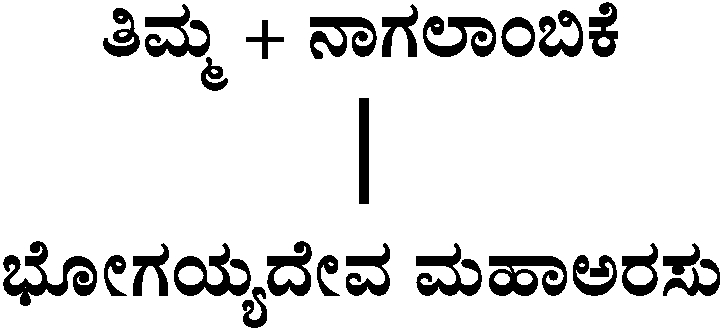
\includegraphics[scale=1.1]{images/chap3/chap3fig39.jpeg}
\end{figure}

\textbf{ಉದಯಗಿರಿಯ ಹರಿನೀಲ ಅಬ್ಬರಾಜನ\index{ಉದಯಗಿರಿಯ ಹರಿನೀಲ ಅಬ್ಬರಾಜ} ಮಗ ತಿರುಮಲರಾಜು\index{ತಿರುಮಲರಾಜು} (1535):} ಅಚ್ಯುತದೇವ ರಾಯನ ಆಳ್ವಿಕೆಯ ಕಾಲದಲ್ಲಿ, ಕಾಶ್ಯಪಗೋತ್ರದ \textbf{“ಸಿಂಧುಗೋವಿಂದ ಶಿತಕರಗಂಡ ಧವಳಂಕಭೀಮ ಮಣಿನಾಗಪುರವರಾಧೀಶ್ವರ\index{ಮಣಿನಾಗಪುರವರಾಧೀಶ್ವರ} ಸ್ವರ್ಗಮರ್ತ್ಯ\-ಪಾತಾಳ ತ್ರಿಭುವನೀರಾಯ ಕಠಾರಿರಾಯ”} ಉದಯಗಿರಿಯ ಹರಿನೀಲ ಅಬ್ಬರಾಜಗಳ ಮಕ್ಕಳು ತಿರುಮಲರಾಜನು, ಚೆಲುವ\-ಪಿಳ್ಳೆರಾಯರ ಪೂಜಾಕೈಂಕರ್ಯಗಳಿಗೆ ಹಳ್ಳಿಗಳನ್ನು ದತ್ತಿ ಬಿಡುತ್ತಾನೆ.\endnote{ ಎಕ 6 ಪಾಂಪು 125 ಮೇಲುಕೋಟೆ 1535} ಮೇಲುಕೋಟೆಯಲ್ಲಿ\index{ಮೇಲುಕೋಟೆ} ಈತನು ಹೊಸದಾಗಿ ತೆಪ್ಪಕೊಳದ\index{ತೆಪ್ಪಕೊಳ} ಮಂಟಪವನ್ನು ಕಟ್ಟಿಸಿದನೆಂದು, ಹಿಂದೆ ಇವನ ತಮ್ಮ ಪೇಟಿ(ರಿ)ರಾಜಯ್ಯನು\index{ಪೇಟಿ(ರಿ)ರಾಜಯ್ಯ} ಕೆರೆಯನ್ನು ಕಟ್ಟಿಸಿದ್ದನೆಂದು ಈ ಶಾಸನದಲ್ಲಿ ಹೇಳಿದೆ. ಮೇಲುಕೋಟೆಯ ಕ್ರಿ.ಶ.1534ರ ಶಾಸನದಲ್ಲಿ ಈತನನ್ನು ಹರಿಗಿಲ ಅಬ್ಬರಾಜಗಳ ಮಕ್ಕಳು ಪೆರಿರಾಜು ಎಂದು ಹೇಳಿದ್ದು, ಈತನು ಚೆಲುವಪಿಳ್ಳೆರಾಯರ\index{ಚೆಲುವಪಿಳ್ಳೆರಾಯ} ತಿರುವಿಡಿಯಾಟದ ಸೀಮೆಯೊಳಗಿನ\index{ತಿರುವಿಡಿಯಾಟದ ಸೀಮೆ} ಕದಳಗೆರೆಯ\index{ಕದ್ದಳಗೆರೆ(ಕದಲಗೆರೆ)} (ಕದಳಗೆರೆ) ಹೊಸಕೆರೆಯೂ, ಕೃಷ್ಣದೇವೊಡೆಯರ ಕೆರೆಯೂ\index{ಕೃಷ್ಣದೇವೊಡೆಯರ ಕೆರೆ} ಒಡೆದು ಖಿಲವಾಗಿರಲು ಅದನ್ನು ಪುನಃ ಕಟ್ಟಿಸಿದನೆಂದು ಹೇಳಿದೆ.\endnote{ ಎಕ 6 ಪಾಂಪು 138 ಮೇಲುಕೋಟೆ 1534} ಈತನು ಉದಯಗಿರಿಯಲ್ಲಿ (ಮಣಿನಾಗಪುರ?) ಮಹಾಮಂಡಲೇಶ್ವರನಾಗಿದ್ದು ಮೇಲುಕೋಟೆಗೆ ಬಂದಿದ್ದಾಗ ಈ ದಾನದತ್ತಿಗಳನ್ನು ನೀಡಿರಬಹುದೆಂದು ಊಹಿಸಹುದು. ಕೃಷ್ಣದೇವ ಒಡೆಯರ ಕೆರೆಯನ್ನು ಕೃಷ್ಣದೇವರಾಯನು ನಿರ್ಮಿಸಿರಬಹುದೆಂದು, ಶಿವನಸಮುದ್ರ, ಶಿವಗಂಗೆಗೆ ಬಂದಿದ್ದಾಗ ಅವನು ಮೇಲುಕೋಟೆಗೂ\index{ಮೇಲುಕೋಟೆ} ಭೇಟಿ ನೀಡಿದ್ದನೆಂದು ಊಹಿಸಹುದು. ಇಲ್ಲೇ ಇರುವ ಇನ್ನೊಂದು ತ್ರುಟಿತ ಶಾಸನದಲ್ಲಿ ತಿರುಮಲರಾಜನು, ಅಚ್ಯುತರಾಯನಿಗೆ\index{ಅಚ್ಯುತರಾಯ} ಬಿನ್ನಹ ಮಾಡಿಕೊಂಡು ಒಂದು ಗ್ರಾಮವನ್ನು ದತ್ತಿ ಬಿಟ್ಟಂತೆ ತಿಳಿದುಬರುತ್ತದೆ.\endnote{ ಎಕ 6 ಪಾಂಪು 127 ಮೇಲುಕೋಟೆ 1534} “ಬೆಲೂರಿನ ನಾಯಕರೂ\index{ಬೆಲೂರಿನ ನಾಯಕರು} ಕೂಡಾ ಮಣಿನಾಗಪುರವರಾಧೀಶ್ವರ\index{ಮಣಿನಾಗಪುರವರಾಧೀಶ್ವರ} ಸಿಂಧಗೋವಿಂದ ಧವಳಾಂಕಭೀಮ\break ಸಿತಕರಗಂಡ ಮತ್ತು ಬರೀದಸಪ್ತಾಂಗಹರಣ ಎಂಬ ಬಿರುದನ್ನು ಧರಿಸಿದ್ದರೆಂದೂ, ಈ ಮನೆತನದ ಮೂಲರಾಜರು\break ಯಲಬುರ್ಗಿಯ ಸಿಂಧ ಮನೆತನದವರೆಂದು, ಮಣಿನಾಗಪುರ ಎಂಬುದು ಬಾದಾಮಿ ತಾಲ್ಲೂಕಿನ ಮಣಿನಾಗರಗ್ರಾಮವೆಂದು” ಎಪಿಗ್ರಾಫಿಯಾ ಕರ್ನಾಟಿಕಾದ ಸಂಪಾದಕರು ಹೇಳಿದ್ದಾರೆ.\endnote{ ಎಪಿಗ್ರಾಫಿಯಾ ಕರ್ನಾಟಿಕಾ, ಸಂಪುಟ 9, ಪೀಠಿಕೆ, ಪುಟ \engfoot{lxxiii – lxxv}} ಆದರೆ ಮೇಲೆ ಉಲ್ಲೇಖಿಸಿದ ಮೇಲುಕೋಟೆ\index{ಮೇಲುಕೋಟೆ} ಶಾಸನದಲ್ಲಿ ಬರುವ ತ್ರಿಭುವನೀರಾಯ ಕಠಾರಿರಾಯರಾದ ಉದಯಗಿರಿಯ ಹರಿನೀಲ ಅಬ್ಬರಾಜಗಳ\index{ಉದಯಗಿರಿಯ ಹರಿನೀಲ ಅಬ್ಬರಾಜ} ಮಕ್ಕಳು ತಿರುಮಲರಾಜನ\index{ತಿರುಮಲ ರಾಜ (ರಾಜಯ್ಯ)} ಹೆಸರು ಎಪಿಗ್ರಾಫಿಯಾ ಸಂಪಾದಕರು ನೀಡಿರುವ ಬೇಲೂರು ನಾಯಕರ ವಂಶಾವಳಿ\-ಯಲ್ಲಿ ಕಂಡುಬರುವುದಿಲ್ಲ. (ಎಕ 9 ಪೀಠಿಕೆ, ಪುಟ lXXV) ಆದರೆ ಬೇಲೂರಿನ ನಾಯಕರಿಗೂ, ಅಬ್ಬರಾಜಗಳ ಮಗ ತಿರುಮಲರಾಜನಿಗೂ ಇವರಿಗೂ ಸಂಬಂಧ ಇರುವಂತೆ ತೋರುತ್ತದೆ.
\begin{figure}[H]
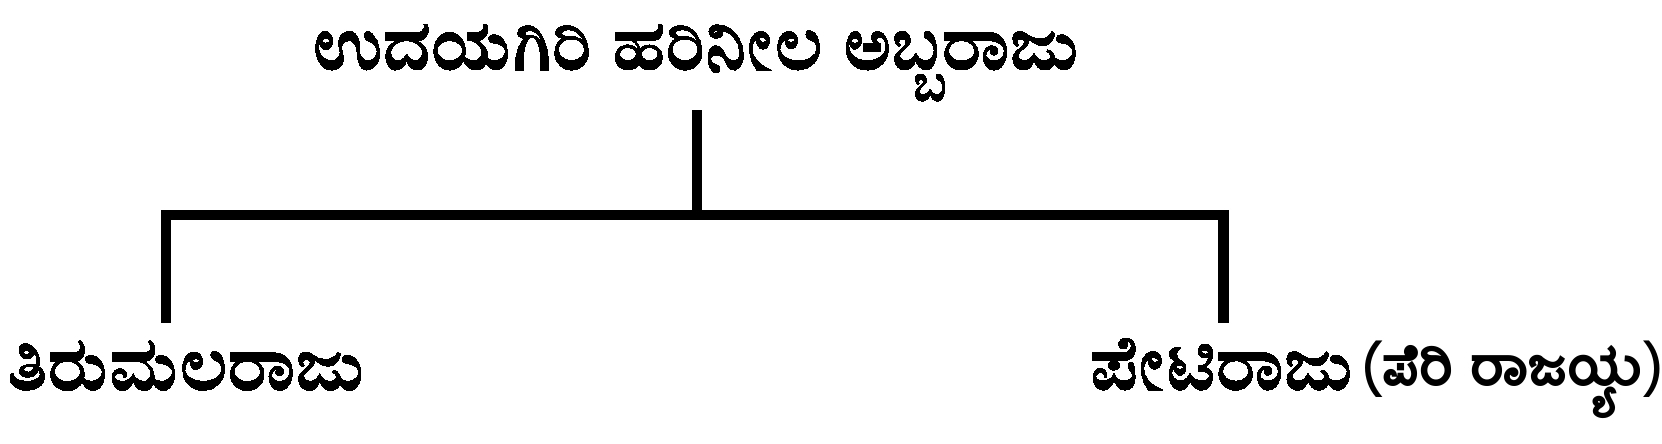
\includegraphics[scale=.15]{images/chap3/chap3fig40.jpeg}
\end{figure}

\textbf{ಮಹಾಮಂಡಲೇಶ್ವರ ನಂದ್ಯಾಲದ ನಾರಯದೇವ ಮಹಾಅರಸ\index{ನಂದ್ಯಾಲದ ನಾರಪ್ಪರಾಜಯ್ಯ (ನಾರಯದೇವ ಮಹಾಅರಸ)} (1545):} ಆತ್ರೇಯ ಗೋತ್ರದ, ಆಪಸ್ತಂಭ ಸೂತ್ರದ, ಯಜುಶಾಖೆಯ, ಮಹಾಮಂಡಲೇಶ್ವರ ನಂದ್ಯಾಲದ ನರಸಿಂಗಯ್ಯದೇವ ಮಹಾ ಅರಸುಗಳ ಕೊಮಾರರು ನಾರಯ್ಯದೇವ ಮಹಾ ಅರಸುಗಳು\index{ನಾರಯ್ಯದೇವ ಮಹಾ ಅರಸು}, ಸದಾಶಿವರಾಯ\index{ಸದಾಶಿವರಾಯ (ದೇವರಾಯ) (ಮಹಾರಾಯ)} ಮಹಾರಾಯನು, ತಮ್ಮ ನಾಯಕತನಕ್ಕೆ ಪಾಲಿಸಿದ ಶ‍್ರೀರಂಗಪಟ್ಟಣ ಸೀಮೆಯೊಳಗಣ\index{ಶ‍್ರೀರಂಗಪಟ್ಟಣ ಸೀಮೆ} ಬಲ್ಲಾಳಪುರದ ಸ್ಥಳ\index{ಬಲ್ಲಾಳಪುರದ ಸ್ಥಳ}, ವರಾಹನಕಲ್ಲಹಳ್ಳಿ ಸ್ಥಳ\index{ವರಾಹನಕಲ್ಲಹಳ್ಳಿ ಸ್ಥಳ} ಹಾಗೂ ಅದಕ್ಕೆ ಸೇರಿದ ಕಾಲುವಳ್ಳಿಗಳನ್ನು ಯಾದವಗಿರಿ (ಮೇಲುಕೋಟೆ) ನಾರಾಯಣದೇವರು ಮತ್ತು ಚೆಲುವಪಿಳ್ಳೆದೇವರಿಗೆ ತಮ್ಮ ಧರ್ಮವಾಗಿ ಪಿನಾಕಿನಿಯ ತೀರದಲ್ಲಿ ಧಾರೆಯ\-ನೆರೆದು ದತ್ತಿಯಾಗಿ ಬಿಡುತ್ತಾನೆ.\endnote{ ಎಕ 6 ಪಾಂಪು 129 ಮೇಲುಕೋಟೆ 1545 ಅಕ್ಟೋಬರ್​ 15} ಇದೇ ನಾರಯದೇವನು ಶ‍್ರೀ ಭಾಷ್ಯಕಾರರು\index{ಶ‍್ರೀ ಭಾಷ್ಯಕಾರರು} ಬಿಜೆಯಮಾಡಿದ್ದ ಯತಿರಾಜಮಠವನು\index{ಯತಿರಾಜಮಠ} ಚೆಲುವಪಿಳ್ಳೆರಾಯರ\index{ಚೆಲುವಪಿಳ್ಳೆರಾಯ} ದೇವಾಲಯಕ್ಕೆ ದೇಶಾಂತ್ರಿ ಮುದ್ರೆಯನ್ನು\index{ದೇಶಾಂತ್ರಿ ಮುದ್ರೆ} ಹಾಕಿಕೊಡುತ್ತಾನೆ. ಶ‍್ರೀಭಂಡಾರವೂ\index{ಶ‍್ರೀಭಂಡಾರ} ಸೇರಿದಂತೆ, ಸೀಮೆಯ ಗ್ರಾಮಗಳ ಕಾಣಿಕೆಯ ಆದಾಯವನ್ನು ಸದಾಶಿವದೇವ ಮಹಾರಾಯರಿಗೆ ಪುಣ್ಯವಾಗಬೇಕೆಂದು ಉಭಯವೇದಾಂತಾಚಾರ್ಯ\index{ಉಭಯ ವೇದಾಂತಾಚಾರ್ಯ} ಕಂದಾಡಿ ಅಣ್ಣನವರ\index{ಕಂದಾಡಿ ಅಣ್ಣ} ಶಿಷ್ಯ ವೇದಾಂತಿ ರಾಮಾನುಜ ಜೀಯನಿಗೆ\index{ವೇದಾಂತದ ರಾಮಾನುಜ ಜೀಯ (ಜೀಯರ್)} ದತ್ತಿಯಾಗಿ ಬಿಡುತ್ತಾನೆ.\endnote{ ಎಕ 6 ಪಾಂಪು 130 ಮೇಲುಕೋಟೆ 1544 ಅಕ್ಟೋಬರ್​ 27}

ಮಹಾಮಂಡಲೇಶ್ವರ ನಂದ್ಯಾಲದ ನಾರಪ್ಪರಾಜಯ್ಯನು\index{ನಂದ್ಯಾಲದ ನಾರಪ್ಪರಾಜಯ್ಯ (ನಾರಯದೇವ ಮಹಾಅರಸ)} ಹದಿನಾಡು ಸೀಮೆಯನ್ನು ಆಳುತ್ತಿದ್ದಾಗ, ತಿಮ್ಮರಾಜಯ್ಯ\index{ತಿಮ್ಮರಾಜಯ್ಯ}, ನಾರಿಯಪ್ಪ ರಾಜಯ್ಯ, ಅಹುಬಳರಾಜಯ್ಯನಿಗೆ\index{ಅಹುಬಳರಾಜಯ್ಯ} ಪುಣ್ಯವಾಗಬೇಕೆಂದು, ನಾರಪ್ಪರಾಜಯ್ಯನ ಕಾರ್ಯಕರ್ತನಾದ ಕಂಪಂಣಗಳು ಕುಂತೂರುಮಠದ ಕೆಂಪನಂಜೇದೇವರಿಗೆ\index{ಕುಂತೂರುಮಠದ ಕೆಂಪನಂಜೇದೇವರು} ಮೂವತ್ತು ವರಹವನ್ನು ದತ್ತಿಯಾಗಿ ಬಿಡುತ್ತಾರೆ.\endnote{ ಎಕ 4 ಕೊಳ್ಳೇಗಾಲ 9 ಕುಂತೂರು 1544} ಈ ಮೂರು ಜನರೂ ನಂದ್ಯಾಲದ ನಾರಸಿಂಗಯ್ಯದೇವನ ಮಕ್ಕಳಾಗಿರಬಹುದು. ಮಹಾಮಂಡಲೇಶ್ವರ, ರಾಜರಾಜ, ನಂದ್ಯಾಲದ ನಾರಪ್ಪರಾಜ ಮಹಾ ಅರಸನ ಕಾರ್ಯಕೆಕರ್ತನಾದ, ಹದಿನಾಡ ಚಾಮರಸಗೌಡನು (ಚಾಮರಾಜ ಒಡೆಯ?) ಮಹಾಮಹತ್ತಿನ ಮಳವಳ್ಳಿಯ ಸಿಂಹಾಸನಕೆ\index{ಮಹಾಮಹತ್ತಿನ ಮಳವಳ್ಳಿಯ ಸಿಂಹಾಸನ} ಕರ್ತರಾದ ನಿಲವಂದದೇವರಿಗೆ (ಮಠಾಧಿಪತಿ) ಹದಿನಾಡು ಸೀಮೆಯ\index{ಹದಿನಾಡು ಸೀಮೆ} ಕೋಳಿಗಾಲ ಸ್ಥಳದ ಹೊಂಡರಬಾಳು\index{ಹೊಂಡರಬಾಳು} ಗ್ರಾಮವನ್ನು ಕ್ರಿ.ಶ. 1549ರಲ್ಲಿ ದತ್ತಿಯಾಗಿ ಬಿಡುತ್ತಾನೆ.\endnote{ ಎಕ 4 ಕೊಳ್ಳೇಗಾಲ 90 ಹೊಂಡರಬಾಳು 1549} ಮಹಾಮಂಡಲೇಶ್ವರ ನಂದ್ಯಾಲದ ತಿಮ್ಮಯ್ಯದೇವ ಮಹಾಅರಸನ ಕಾರ್ಯಕೆಕರ್ತನಾದ ವೆಂಗಳರಾಜಯ್ಯನು ಅಣಿಲೇಶ್ವರ ಲಿಂಗಕ್ಕೆ\index{ಅಣಿಲೇಶ್ವರ} ದತ್ತಿ ಬಿಡುತ್ತಾನೆ.\endnote{ ಎಕ 4 ಚಾಮರಾಜನಗರ 234 ಭಂಡಿಗೆರೆ 16ನೇ ಶ.} ಪೂರ್ವೋಕ್ತ ಶಾಸನದ ತಿಮ್ಮರಾಜ, ತಿಮ್ಮಯ್ಯದೇವ ಇವರು ಅಭಿನ್ನರಿದ್ದು ಇವನು ನಾರಯ್ಯದೇವನ ಸಹೋದರನಾಗಿರಬಹುದು. ಸಿ. ಹಯವದನರಾವ್​ ಅವರು ನಂದ್ಯಾಲದ ನಾರಸಿಂಗದೇವನ ವಂಶಾವಳಿಯನ್ನು ಈ ರೀತಿ ಕಟ್ಟಿಕೊಟ್ಟಿದ್ದಾರೆ.\endnote{ ಹಯವದನರಾವ್​, ಸಿ., ಮೈಸೂರು ಗೆಜೆಟಿಯರ್​, ಸಂಪುಟ 2, ಭಾಗ 3. ಪುಟ 2422} ತಿಮ್ಮರಾಜನ ಹೆಸರು ಈ ವಂಶಾವಳಿಯಲ್ಲಿ ಇಲ್ಲ.

\begin{figure}[H]
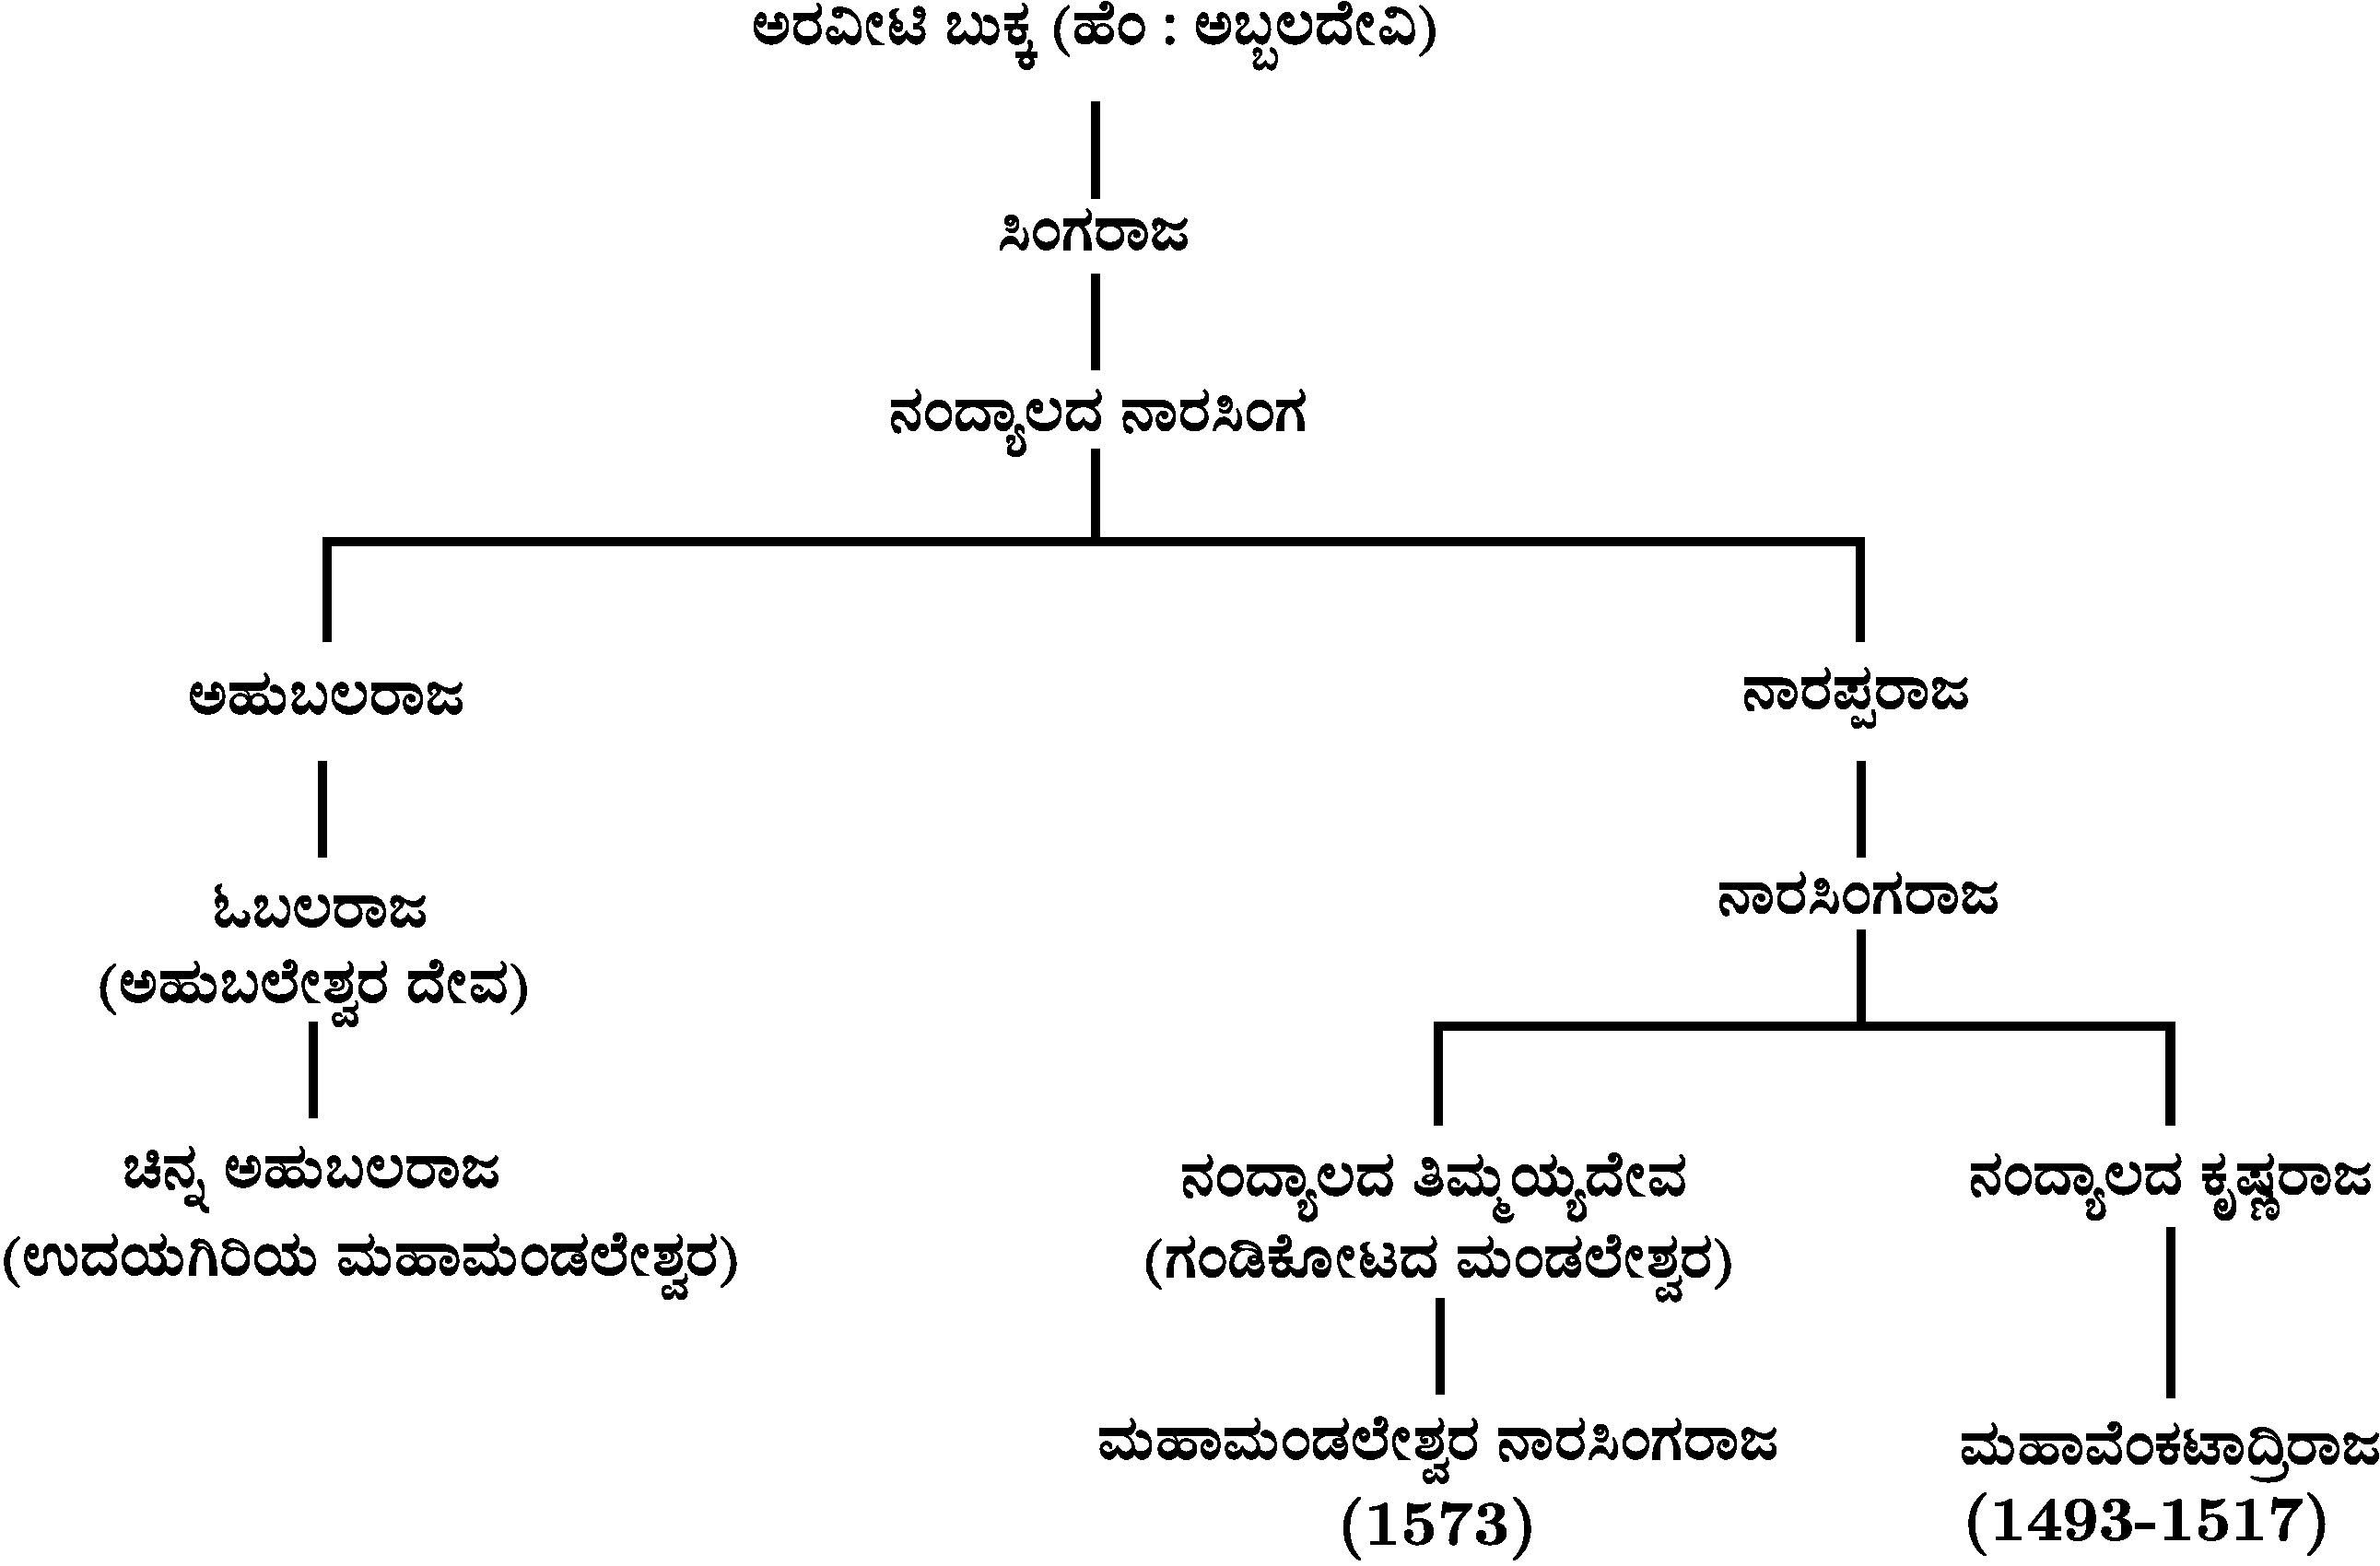
\includegraphics[scale=1.2]{images/chap3/chap3fig41.jpeg}
\end{figure}

\textbf{ಮಹಾಮಂಡಲೇಶ್ವರ ರಾಮರಾಜ ಮಹಾಅರಸು\index{ರಾಮರಾಜ ಮಹಾ ಅರಸು}(ರಾಮರಾಜಯ್ಯದೇವ ಮಹಾಅರಸು\index{ರಾಮರಾಜಯ್ಯ (ದೇವ - ಮಹಾ ಅರಸು), ರಾಮರಾಜವೊಡೆಯ }) ಮತ್ತು ಅವನ ವಂಶಸ್ಥರು:} ಅರವೀಡು ವಂಶದ ಒಂದನೆಯ ಶ‍್ರೀರಂಗನ ಮಗ ರಾಮರಾಯ (ಅಳಿಯರಾಮರಾಯ\index{ಅಳಿಯ ರಾಮರಾಯ}) ನಿಗೆ ತಿರುಮಲನೆಂಬ\index{ತಿರುಮಲ} ತಮ್ಮನಿದ್ದನು. ಈತನು ಕ್ರಿ.ಶ.1570 ರಿಂದ 1578ರವರೆಗೆ ಆಳ್ವಿಕೆ ನಡೆಸಿದನು. ಆದರೆ ಇವನು ಕ್ರಿ.ಶ.1565ರಿಂದಲೇ ಸದಾಶಿವರ ರಾಯನು\index{ಸದಾಶಿವರಾಯ (ದೇವರಾಯ) (ಮಹಾರಾಯ)} ಬದುಕಿದ್ದಾಗಲೇ, ಅವನನ್ನು ಹಿಂದಿಕ್ಕಿ ಅಥವಾ ಕಾರಾಗೃಹದಲ್ಲಿಟ್ಟು ಅವನ ಹೆಸರಿನಲ್ಲಿಯೇ ಆಡಳಿತ ನಡೆಸುತ್ತಿದ್ದನೆಂದು ತಿಳಿದುಬರುತ್ತದೆ.\endnote{ ದೇಸಾಯಿ, ಡಾ॥ ಪಿ.ಬಿ., ವಿಜಯನಗರ ಸಾಮ್ರಾಜ್ಯ, ಪುಟ 138} ಇವನ ಮಗ ಇಮ್ಮಡಿ ಶ‍್ರೀರಂಗ\index{ಇಮ್ಮಡಿ ಶ‍್ರೀರಂಗ}. ಇವನು 1578 ರಿಂದ 1585ರವರೆಗೆ ಆಳ್ವಿಕೆ ನಡೆಸಿದನು. ಇವನ ತಮ್ಮ ರಾಮ ಅಥವಾ ರಾಮದೇವ. ರಾಮನ ತಮ್ಮ ವೆಂಕಟಪತಿಯು\index{ವೆಂಕಟಪತಿಮಹಾರಾಯ} 1585 ರಿಂದ 1614ರವರೆಗೆ ಆಳ್ವಿಕೆ ನಡೆಸಿದರು ಎಂದು ಪಿ.ಬಿ. ದೇಸಾಯಿ ಅವರು ಹೇಳಿದ್ದಾರೆ.\endnote{ ದೇಸಾಯಿ, ಡಾ. ಪಿ.ಬಿ., ವಿಜಯನಗರ ಸಾಮ್ರಾಜ್ಯ, ಪುಟ 265}

ರಾಮ ಅಥವಾ ರಾಮದೇವನು ನೇರವಾಗಿ ರಾಜ್ಯವನ್ನು ಆಳದೇ ಹೋದರೂ, ಶ‍್ರೀರಂಗಪಟ್ಟಣದಿಂದ\index{ಶ‍್ರೀರಂಗಪಟ್ಟಣ} ಯುವರಾಜ ಅಥವಾ ಮಾಂಡಲೀಕನಾಗಿ ಆಳ್ವಿಕೆ ನಡೆಸುತ್ತಿದ್ದಿರಬಹುದು. ಶ‍್ರೀರಂಗಪಟ್ಟಣ ಶಾಸನವು \textbf{“ಶ‍್ರೀಮನ್​ ಮಹಾರಾಜಾಧಿರಾಜ ರಾಜಪರಮೇಶ್ವರ ಶ‍್ರೀ ವೀರಪ್ರತಾಪ ತಿರುಮಲದೇವ ಮಹಾರಾಯರ ಕೊಮಾರ ರಾಮರಾಜಯರ್ಸರು}” ಎಂದು ಹೇಳಿದೆ.\endnote{ ಎಕ 6 ಶ‍್ರೀಪ 6 ಶ‍್ರೀರಂಗಪಟ್ಟಣ 1571} “ಶಾಸನದ ಕಾಲದಂದು ಅಳಿಯ ರಾಮರಾಯನ ಸೋದರ ತಿರುಮಲನು ಆಳುತ್ತಿದ್ದರೂ, ಆತನ ಮಗ ರಾಮನು ಮೈಸೂರು ಸುತ್ತಲಿನ ಪ್ರದೇಶದ ಅಧಿಕಾರಿಯಾಗಿದ್ದನೆಂದು ಇತರ ಆಧಾರಗಳಿಂದ ತಿಳಿದಿದೆಯಾಗಿ, ಶಾಸನೋಕ್ತ ರಾಮರಾಜ ಈ ರಾಮನೇ ಆಗಿರಬಹುದು” ಎಂದು ಎಪಿಗ್ರಾಫಿಯಾ ಸಂಪಾದಕರು ಅಭಿಪ್ರಾಯಪಟ್ಟಿರುವುದು ಸೂಕ್ತವಾಗಿದೆ.\endnote{ ಎಪಿಗ್ರಾಫಿಯಾ ಕರ್ನಾಟಿಕಾ, ಸಂಪುಟ 6 ಪೀಠಿಕೆ, ಪುಟ ಟತ್i} ರಾಮರಾಜಯ್ಯನು ವೆಂಕಟಪತಿಮಹಾರಾಯರ\index{ವೆಂಕಟಪತಿಮಹಾರಾಯ} ಅಣ್ಣನೆಂದು ಬೆಳಗೊಳ ಶಾಸನದಲ್ಲಿ ಹೇಳಿದೆ.\endnote{ ಎಕ 6 ಶ‍್ರೀಪ 71 ಬೆಳಗೊಳ 1598} ಮಹಾಮಂಡಲೇಶ್ವರ ರಾಮರಾಜಯ್ಯನ ತಮ್ಮ ತಿರುವೆಂಕಟಾದ್ರಿ ಮಹಾ ಅರಸನೆಂದು\index{ತಿರುವೆಂಕಟಾದ್ರಿ ಮಹಾ ಅರಸ} ಹಿರೆಜಂತಕಲ್​ ಶಾಸನದಿಂದ ತಿಳಿದುಬರುತ್ತದೆ.\endnote{ ಕವಿವಿ ಶಾಸಂ 2 ಗಂಗಾವತಿ 3 ಹಿರೆಜಂತಕಲ್​ 1544} ಇಮ್ಮಡಿ ಶ‍್ರೀರಂಗನ(1578\enginline{-}1585) ನಂತರ ರಾಜ್ಯವಾಳಿದ ವೆಂಕಟಪತಿಯೇ(1585\enginline{-}1614) ಈ ವೆಂಕಟಪತಿಮಹಾರಾಯ ಅಥವಾ ವೆಂಕಟಾದ್ರಿ ಮಹಾಅರಸ\-ನಾಗಿದ್ದಾನೆ. ಇದರಿಂದ ರಾಮರಾಜಯ್ಯನು ಒಂದನೆಯ ತಿರುಮಲನ\index{ಒಂದನೆಯ ತಿರುಮಲ} ಮಗನೆಂದೂ, ವೆಂಕಟಾದ್ರಿ ಮಹಾಅರಸನ ಅಣ್ಣ\-ನೆಂಬುದೂ ಖಚಿತವಾಗುತ್ತದೆ. ಪಿ.ಬಿ.ದೇಸಾಯಿ ಅವರು ನೀಡಿರುವ ಅರವೀಡು ಮನೆತನದ ವಂಶವೃಕ್ಷ ಈ ರೀತಿ ಇದೆ.\endnote{ ದೇಸಾಯಿ, ಡಾ॥ ಪಿ.ಬಿ., ವಿಜಯನಗರ ಸಾಮ್ರಾಜ್ಯ, ಪುಟ 265}

\newpage

\begin{figure}[H]
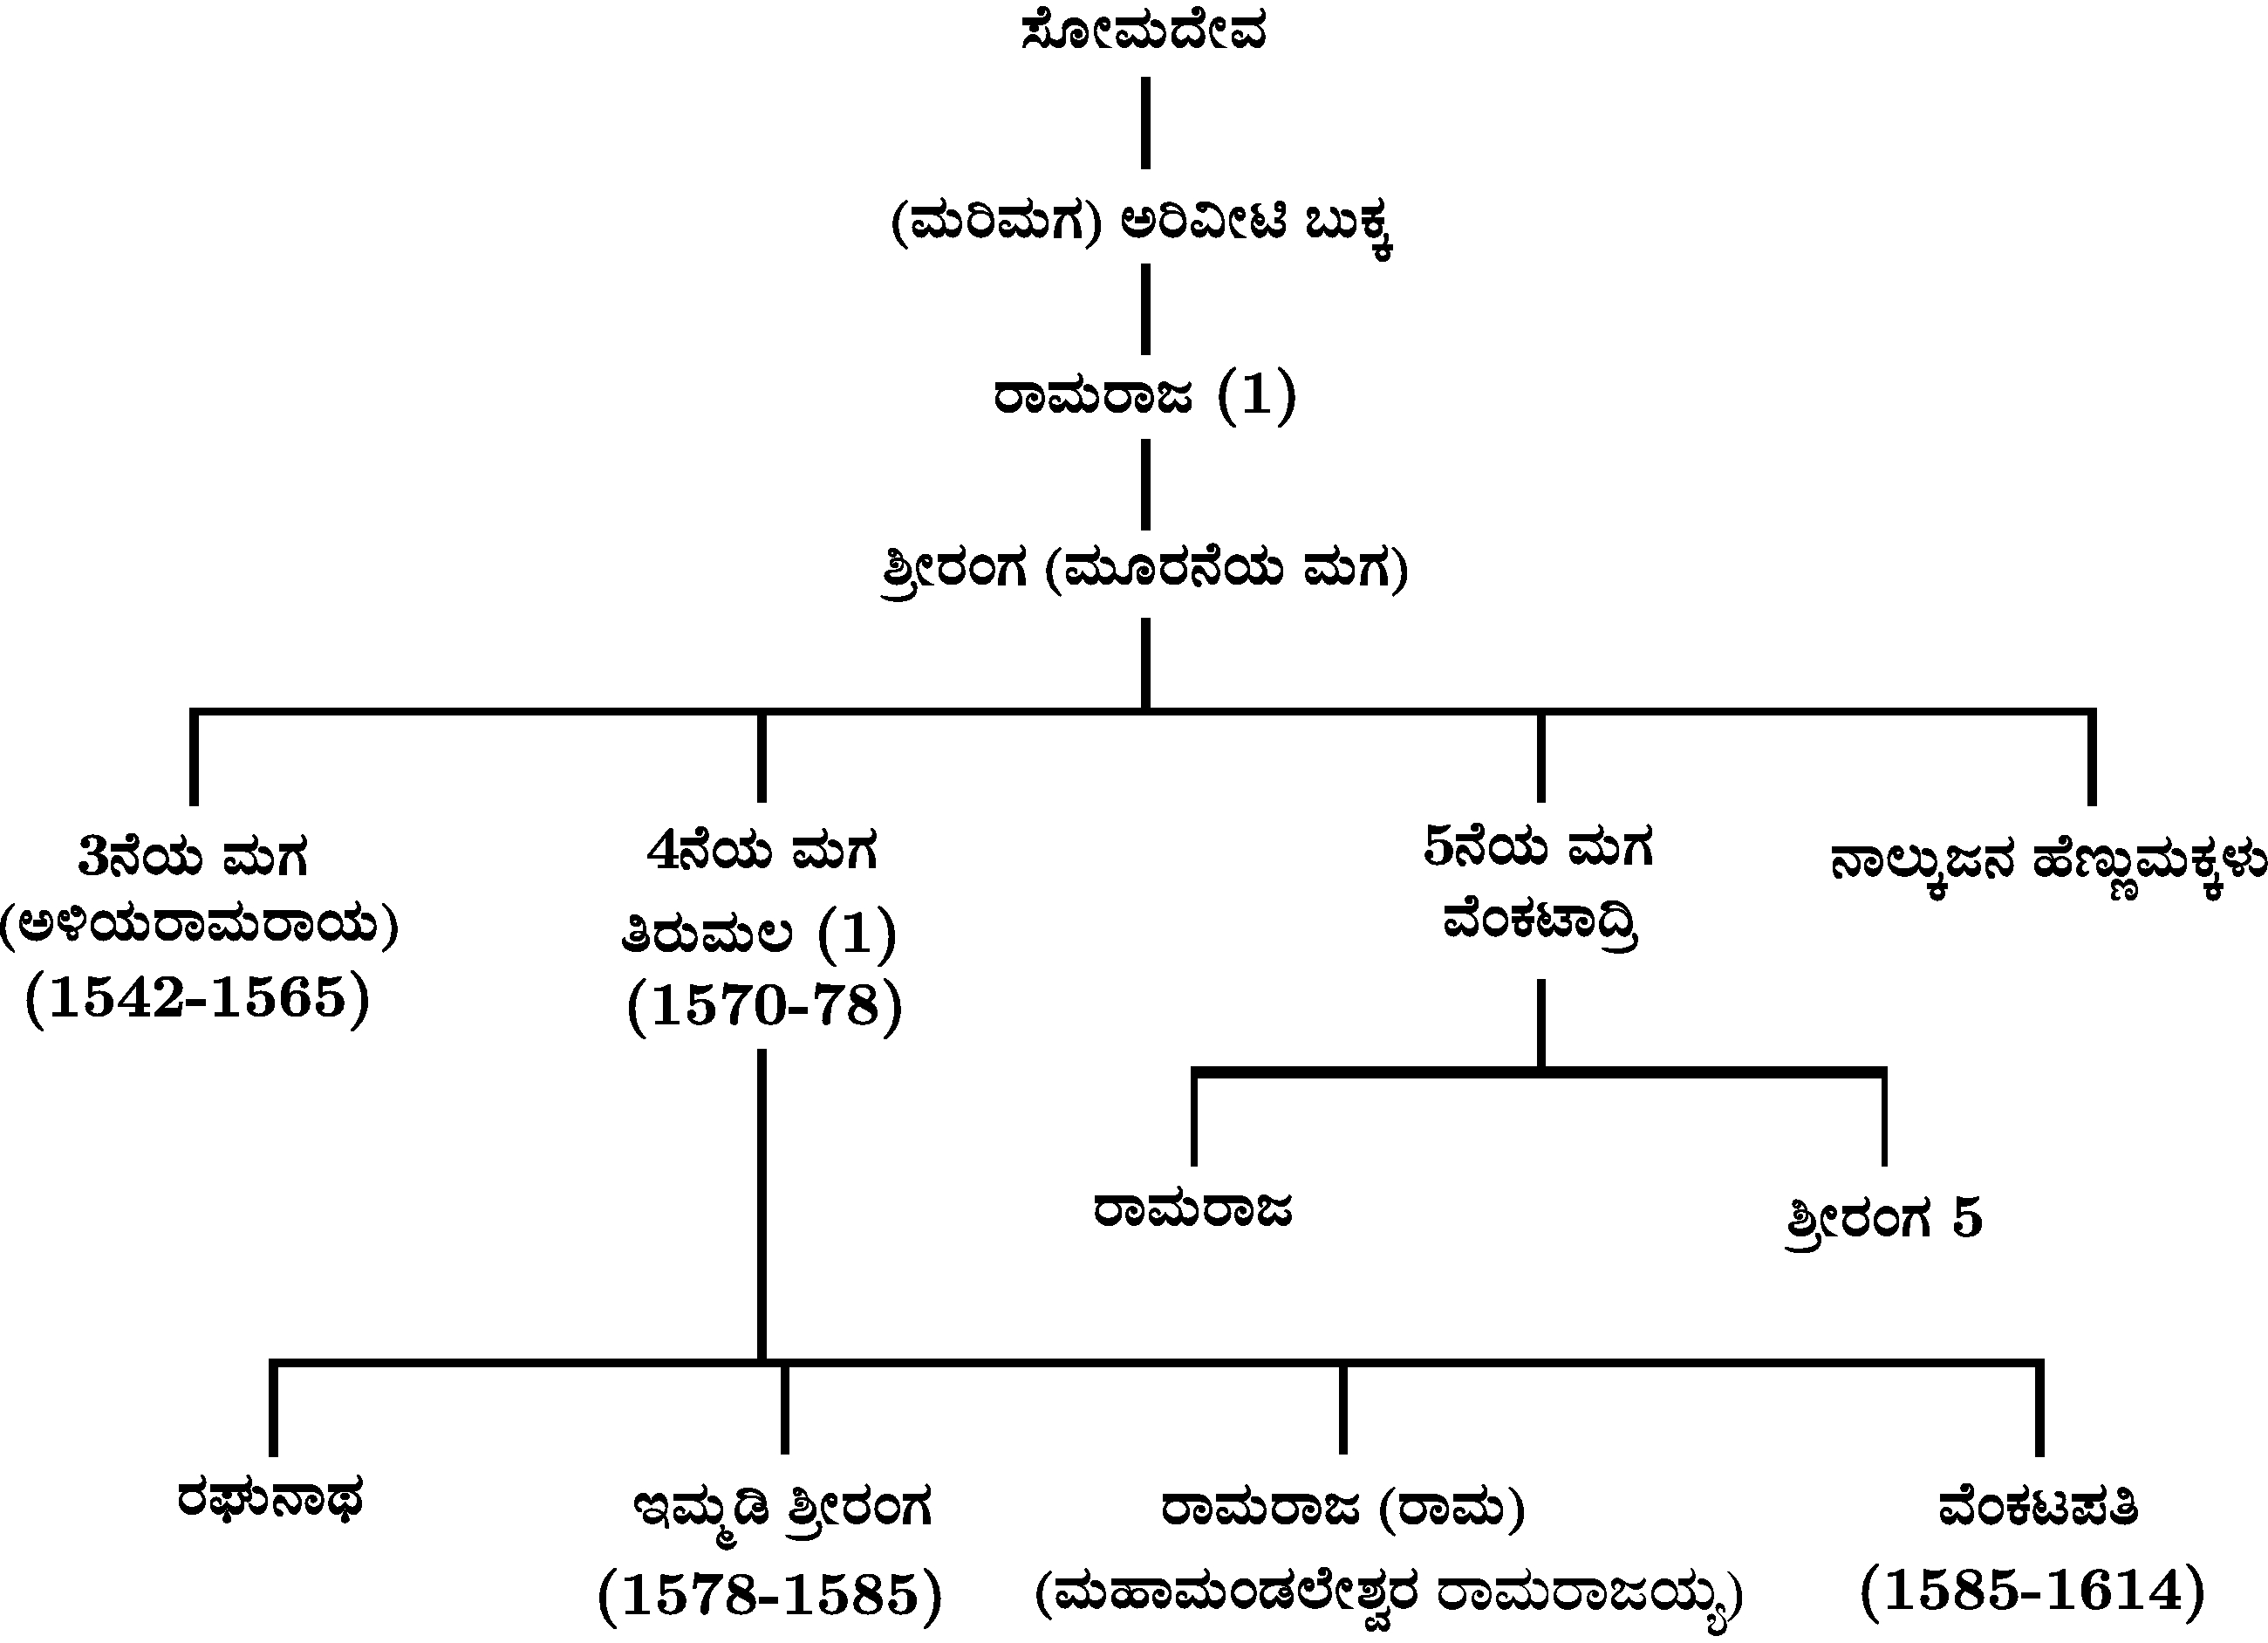
\includegraphics[scale=1.2]{images/chap3/chap3fig42.jpeg}
\end{figure}

ವೆಂಕಟಾದ್ರಿ ಮಹಾಅರಸನಿಗೂ ತಿರುಮಲನೆಂಬ ಮಗನಿದ್ದನು. “ವೀರಪ್ರತಾಪ ವೆಂಕಟಪತಿರಾಯರ ಕುಮಾರ\break ತಿರುಮಲರಾಜಯ್ಯ\index{ತಿರುಮಲ ರಾಜ (ರಾಜಯ್ಯ)}”ನು ತ್ರಿಯಂಬಕೇಶ್ವರ ದೇವರ\index{ತ್ರಿಯಂಬಕೇಶ್ವರ ದೇವರು} ಅಭಿಷೇಕಕ್ಕೆ ಬಾವಿಯನ್ನು ತೋಡಿಸಿದ್ದನೆಂದೂ, ಅದನ್ನು\break ಕಂಠೀರವ ನರಸರಾಜನು ಜೀರ್ಣೋದ್ಧಾರ ಮಾಡಿದನೆಂದೂ ತ್ರಿಯಂಬಕಪುರ ಶಾಸನದಿಂದ ತಿಳಿದುಬರುತ್ತದೆ.\endnote{ ಎಕ 3 ಗುಂಡ್ಲುಪೇಟೆ 146 ತ್ರಿಯಂಬಕಪುರ 1645}

ಹಂಪೆಯ ಕೆಲವು ಮೊದಲಿನ ಶಾಸನಗಳು, ರಾಮರಾಜಯ್ಯನನ್ನು\index{ರಾಮರಾಜಯ್ಯ (ದೇವ - ಮಹಾ ಅರಸು), ರಾಮರಾಜವೊಡೆಯ } ಸದಾಶಿವರಾಯನ\index{ಸದಾಶಿವರಾಯ (ದೇವರಾಯ) (ಮಹಾರಾಯ)} ಕಾರ್ಯಕೆಕರ್ತ\index{ಕಾರ್ಯಕೆ ಕರ್ತ} ಎಂದು ಕರೆದಿವೆ.\endnote{ ಕವಿವಿ ಶಾ ಸಂ. 2 ಹಂಪೆ 83 ಮತ್ತು 84, 1545} ಇವನು ಮೊದಲು ಸಣ್ಣ ಹುದ್ದೆಯಲ್ಲಿದ್ದು ನಂತರ ಮಹಾಮಂಡಲೇಶ್ವರ ಪದವಿಗೆ ಏರಿರಬಹುದು. \hbox{ರಾಮರಾಜಯ್ಯನು} ಕ್ರಿ.ಶ.1545 ರಿಂದಲೇ ಶ‍್ರೀರಂಗಪಟ್ಟಣದಿಂದ ಆಳುತ್ತಿದ್ದನೆಂದು ಹೇಳಬಹುದು. ಶ‍್ರೀರಂಗಪಟ್ಟಣದ ಗಂಗಾಧರೇಶ್ವರ\index{ಗಂಗಾಧರೇಶ್ವರ} ದೇವರ ಸಮ್ಮುಖದಲ್ಲಿ ಹದಿನಾಡು ಸೀಮೆಯ\index{ಹದಿನಾಡು ಸೀಮೆ} ನಾಗವಲ್ಲಿ ಮತ್ತು ಕುಂದಘಟ್ಟ ಸ್ಥಳದ ಹಳ್ಳಿಗಳನ್ನು ಸುತ್ತೂರು ಮಠದ ದಾಸೋಹಕ್ಕೆ\index{ದಾಸೋಹ} ದತ್ತಿಯಾಗಿ ಬಿಟ್ಟ ವಿಚಾರವನ್ನು ಹೇಳುವ ಶಾಸನದಲ್ಲಿ ಮಹಾಮಂಡಲೇಶ್ವರನ ಹೆಸರು ಅಳಿಸಿ ಹೋಗಿದ್ದು, ಅದು ರಾಮರಾಜಯ್ಯನ ಶಾಸನವೇ ಆಗಿರುವಂತೆ ತೋರುತ್ತದೆ.\endnote{ ಎಕ 4 ಚಾಮರಾಜನಗರ 217 ಪುಟ್ಟನಪುರ 1545} ರಾಮರಾಜಯ್ಯ ಮಹಾ ಅರಸನು ಕ್ರಿ.ಶ.1550ರಲ್ಲಿ ಶ‍್ರೀರಂಗಪಟ್ಟಣ ಸೀಮೆಯ ನಾಯಕರುಗಳಿಗೆ ಕುಳ ಸುಂಕವನ್ನು\index{ಕುಳ ಸುಂಕ}, ನಾಯಿಂದರುಗಳಿಗೆ\index{ನಾಯಿಂದರು(ನಾವಿದರು)} ಸುಂಕವನ್ನು ಸರ್ವಮಾನ್ಯವಾಗಿ ಬಿಡುತ್ತಾನೆ. ಇದೇ ಮಂಡ್ಯ ಜಿಲ್ಲೆಯಲ್ಲಿ ಸಿಗುವ ರಾಮರಾಜಯ್ಯನ ಮೊದಲನೇ ಶಾಸ.\endnote{ ಎಕ 6 ಪಾಂಪು 237 ಸುಂಕಾತೊಂಡನೂರು 1550} ರಾಮರಾಜಯ್ಯದೇವ ಮಹಾ ಅರಸನು ತನ್ನ ಕಾರ್ಯಕರ್ತ ಅರೆಕೊಠಾರದ ನಾಯಕ ನಂದ್ಯಾಲದ ತಿಮ್ಮರಾಜನಿಗೆ, ಉಡಿಯಗಾಲ ಗ್ರಾಮವನ್ನು ನಾಯಕತನದ ಕೊಡುಗೆಯಾಗಿ ನೀಡಿದ್ದನು.\endnote{ ಎಕ 4 ಚಾಮರಾಜನಗರ 315 ಉಡೀಗಾಲ 1551} ಅರಸೀಕೆರೆ ತಾಲ್ಲೂಕು ಸಿಂಗನಹಳ್ಳಿ ಶಾಸನವು ಇವನ ಪ್ರಶಸ್ತಿಯನ್ನು ನೀಡಿದೆ. \textbf{“ಶ‍್ರೀ ಪ್ರುಥ್ವೀವಲ್ಲಭ ರಾಜಪರಮೇಶ್ವರ ಶ‍್ರೀ ವೀರಪ್ರತಾಪ ಶ‍್ರೀಮನ್ಮಹಾಮಂಡಲೇಶ್ವರ ರಾಮರಾಜ ಮಹಾ ಅರಸುಗಳ\index{ರಾಮರಾಜ ಮಹಾ ಅರಸು} ಪ್ರತಾಪಮೆಂತೆಂದಡೆ ಭುಜಪ್ರತಾಪದಿ ಮಹಾರ್ನ್ನವ ಮೂರರ ಮಧ್ಯದೇಸಮುದ್ದಂಡವಿನಾಳ್ದು ತಂನ ಭುಜಸಾಹಸದಿಂ ಸುರಿತಾಣಭೂಪರಂ ಖಂಡಿಸಿ ಆರ್ಯಮಂಡುನದ ಕೇರಳವಡ್ಡಿಯ ರಾಜರೆಲ್ಲರಂ ತಂಡವತಂದು ಕಯಿಸೆರೆಯನಿಕ್ಕಿದ ರಾಮನ್ರಿಪ ಭೂಪಾಲಂ\index{ರಾಮನ್ರಿಪ ಭೂಪಾಲ}”} ಎಂದು ಹೇಳಿದ್ದು, ಕೊಳುಗುಂದದ ಗವುಡುಗಳು ರಾಮೇಶ್ವರ ದೇವಾಲಯವನ್ನು ಕಟ್ಟಿಸಿದಾಗ ರಾಮರಾಜಯ್ಯನು ಅದಕ್ಕೆ ದತ್ತಿಯನ್ನು ಬಿಟ್ಟ ವಿಷಯವನ್ನು ಹೇಳಿದೆ.\endnote{ ಎಕ 10 ಅರಸೀಕೆರೆ 261 ಸಿಂಗನಹಳ್ಳಿ 1555} ರಾಮರಾಜಯ್ಯ ದೇವ ಮಹಾಅರಸನು ಇಂದಿನ ಬೇಲೂರು ತಾಲ್ಲೂಕಿನ ಮಾದಿಹಳ್ಳಿ ಸೀಮೆಯ\index{ಮಾದಿಹಳ್ಳಿ ಸೀಮೆ} ಮಾದಿಹಳ್ಳಿ ಸ್ಥಳದ ಮೂಳೇನಹಳ್ಳಿಯನ್ನು\index{ಮೂಳೇನಹಳ್ಳಿ} ಪೇಟೆಯನ್ನಾಗಿ ಮಾಡಿ ಚೆನ್ನಕೇಶವ ದೇವರಿಗೆ\index{ಚೆನ್ನಕೇಶವ ದೇವರು} ದತ್ತಿಯಾಗಿ ಬಿಟ್ಟು ಪೇಟೆ ಶಾಸನ ಹಾಕಿಸಿದನು.\endnote{ ಎಕ 9 ಬೇಲೂರು 492 ಮೂಳೇನಹಳ್ಳಿ 1562} ರಾಮರಾಜಯ್ಯನು, ಸದಾಶಿವರಾಯನು ತನಗೆ ಪಾಲಿಸಿದ್ದ ಹಾಸನ ಸೀಮೆಯನ್ನು ಬೇಲೂರಿನ ನಾಯಕನಾದ\index{ಬೇಲೂರಿನ ನಾಯಕ} ಬಯ್ಯಪ್ಪನಾಯಕರ ಮಕ್ಕಳು ಕೃಷ್ಣಪ್ಪನಾಯಕನ\index{ಕೃಷ್ಣಪ್ಪನಾಯಕ} ನಾಯಕತನಕ್ಕೆ ಅಥವಾ ಅಮರಮಾಗಣೆಗೆ\index{ಅಮರಮಾಗಣಿ} ನೀಡಿದ್ದನು. ಈ ಸೀಮೆಯ ಅನೇಕ ಹಳ್ಳಿಗಳನ್ನು ಕೃಷ್ಣಪ್ಪನಾಯಕನು ಗುತ್ತಿಗೆಗೆ ಮತ್ತು ದತ್ತಿಯಾಗಿ ಬಿಟ್ಟ ವಿಚಾರವನ್ನು ಅನೇಕ ಶಾಸನಗಳು ಹೇಳುತ್ತವೆ.\endnote{ ಎಕ 8 ಹಾಸನ 122 ಪುರ 1562, ಹಾಸನ 79 ಕುದುರೆಗುಂಡಿ 1562

ಎಕ 8 ಹಾಸನ 2 ಹಾಸನ 1563} ಶ‍್ರೀಮನ್ಮಹಾಮಂಡಲೇಶ್ವರ ರಾಮರಾಜ ತಿರುಮಲರಾಜ ಅರಸರ ಕೊಮಾರ ರಾಮರಾಜಯ್ಯದೇವ ಮಹಾಅರಸನು ಹದಿನಾಡು ಸೀಮೆಯ ಪ್ರಭು ರಾಮರಾಜನಾಯಕನಿಗೆ\index{ರಾಮರಾಜನಾಯಕ} ಶಿವನಸಮುದ್ರ ಸ್ಥಳದ ಕೋಳೋಗಾಲ (ಕೊಳ್ಳೇಗಾಲ)\index{ಕೋಳೋಗಾಲ (ಕೊಳ್ಳೇಗಾಲ)} ಸ್ಥಳವನ್ನು ಪಲ್ಲಕ್ಕಿ ಉಂಬಳಿಯಾಗಿ\index{ಪಲ್ಲಕ್ಕಿ ಉಂಬಳಿ} ನೀಡಿದನು.\endnote{ ಎಕ 4 ಕೊಳ್ಳೇಗಾಲ 1 ಕೊಳ್ಳೇಗಾಲ 1569} ಶ‍್ರೀಮನ್ಮಹಾರಾಜಾಧಿರಾಜ ರಾಜಪರಮೇಶ್ವರ ಶ‍್ರೀ ವೀರಪ್ರತಾಪ ತಿರುಮಲದೇವ ಮಹಾರಾಯರ ಕುಮಾರ ರಾಮರಾಜಯ್ಯ ಅರಸನು ಸರ್ವೋತ್ತಮ ಒಡೆಯರಿಗೆ\index{ಸರ್ವೋತ್ತಮ ಒಡೆಯ} ಬಣ್ಣಂಗಟ್ಟಿ\index{ಬಣ್ಣಂಗಟ್ಟಿ (ಬನ್ನಂಗಾಡಿ)}(ಪಾಂಡವಪುರ ತಾ. ಬನ್ನಂಗಾಡಿ) ಗ್ರಾಮವನ್ನು ದತ್ತಿಯಾಗಿ ನೀಡಿದನು.\endnote{ ಎಕ 6 ಶ‍್ರೀಪ 6 ಶ‍್ರೀರಂಗಪಟ್ಟಣ 1571}

ಕೆಲವು ಶಾಸನಗಳಲ್ಲಿ ರಾಮರಾಜಯ್ಯನನ್ನು ಶ‍್ರೀರಂಗಗಳ ಕೊಮಾರ ರಾಮರಾಜಯ್ಯನೆಂದು ಹೇಳಿದೆ. “ಶ‍್ರೀಮನ್ಮಹಾ\-ರಾಜಾಧಿರಾಜ ರಾಜಪರಮೇಶ್ವರ ಶ‍್ರೀ ವೀರಪ್ರತಾಪ ಶ‍್ರೀರಂಗರಾಜದೇವ\index{ಶ‍್ರೀರಂಗರಾಜದೇವ} ಮಹಾರಾಯರೂ ಪ್ರುಥ್ವೀರಾಜ್ಯಂಗೆಯುತ್ತಿರಲು ಶ‍್ರೀರಂಗರಾಯರ ಕೊಮಾರ ರಾಮರಾಜ ಮಹಾಅರಸುಗಳು” ಮೇಲುಕೋಟೆಯಲ್ಲಿ\index{ಮೇಲುಕೋಟೆ} ಯತಿರಾಜಸಪ್ತತಿಯನ್ನು\index{ಯತಿರಾಜ ಸಪ್ತತಿ (ಸಪ್ತಶತಿ)} ನಡೆಸಲು ರಾಜನ ನಿರೂಪವನ್ನು ಪಡೆದು ಅದನ್ನು ಸ್ಥಳದ ಅಧಿಕಾರಿ ರಾಮಾನುಜಯ್ಯನಿಗೆ ಕಳುಹಿಸುತ್ತಾರ.\endnote{ ಎಕ 6 ಪಾಂಪು 136 ಮೇಲುಕೋಟೆ 1574} ಅದೇ ರೀತಿ ಸದಾಶಿವರಾಯನ ಕಾಲದಲ್ಲಿಯೂ ಕೂಡಾ “ಶ‍್ರೀಮನ್ಮಹಾಮಂಡಲೇಶ್ವರ ಆತ್ರೇಯಗೋತ್ರದ ಆಪಸ್ತಂಭ ಸೂತ್ರದ ಶ‍್ರೀರಂಗಗಳ ಕೊಮಾರ ರಾಮರಾಜಯ್ಯನವರ” ನಿರೂಪದಿಂದ ದಿಂಮರಾಜಯ್ಯನು\index{ದಿಂಮರಾಜಯ್ಯ} (ರಾಮರಾಜಯ್ಯನ ತಮ್ಮ ಸದಾಶಿವರಾಯನ ಮಂತ್ರಿ ಎರದಿಂಮರಾಜಯ್ಯ\index{ಎರದಿಂಮರಾಜಯ್ಯ}) ರಾವಿಯಹಾಳೆಯ(ಮಲ್ಲಿನಾಥಪುರ) ಅಗ್ರಹಾರದ ತೆರಿಗೆಗಳನ್ನು ದತ್ತಿ ಬಿಡುತ್ತಾನೆ.\endnote{ ಕವಿವಿ ಶಾ ಸಂ. 1 ಬಳ್ಳಾರಿ 25 ರಾವಿಹಾಳು 1576} ಅಳಿಯ ರಾಮರಾಯನ ತಮ್ಮ ತಿರುಮಲನ ಆಳ್ವಿಕೆಯ ನಂತರ, ತಿರುಮಲನ ಮಗ ರಾಮರಾಜಯ್ಯನ ಅಣ್ಣ ಇಮ್ಮಡಿ ಶ‍್ರೀರಂಗನು(1678\enginline{-}1685) ಪಟ್ಟಕ್ಕೆ ಬಂದನು. ಇವನ ಕಾಲದಲ್ಲಿಯೂ ರಾಮರಾಜಯ್ಯನು ಮಹಾಮಂಡಲೇಶ್ವರನಾಗಿ ಆಳ್ವಿಕೆ ನಡೆಸುತ್ತಿದ್ದುದರಿಂದ ಇವನನ್ನು ಶ‍್ರೀರಂಗರಾಯನ ಕೊಮಾರ (ಪ್ರೀತಿಯ ತಮ್ಮ) ಎಂದು ಕರೆದಿರಬಹುದು.

ಮಹಾಮಂಡಲೇಶ್ವರ ರಾಮರಾಜಯ್ಯ ಮಹಾ ಅರಸರುಗಳು ತಳಕಾಡ (ಚಂದ್ರಶೇಖರ ಒಡೆಯರಿಗೆ) ಅರಸನಕೆರೆಯ ಸ್ಥಳದ\index{ಅರಸನಕೆರೆಯ ಸ್ಥಳ} ಕುದುರೆಗುಂಡಿಯನ್ನು\index{ಕುದುರೆಗುಂಡಿ} ಪಲ್ಲಕ್ಕಿ ಉಂಬಳಿಯಾಗಿ\index{ಪಲ್ಲಕ್ಕಿ ಉಂಬಳಿ} ಕೊಡುತ್ತಾನೆ.\endnote{ ಎಕ 7 ಮ 137 ಕುದುರೆಗುಂಡಿ 1576} ಹದಿನಾಡ ರಾಮರಾಜನಾಯಕನಿಗೆ ಉಮ್ಮತ್ತೂರು ಸೀಮೆಯ\index{ಉಮ್ಮತ್ತೂರು ಸೀಮೆ} ಕುದಿಹೆರು(ಕುದೇರು)\index{ಕುದಿಹೆರು(ಕುದೇರು)} ಸ್ಥಳವನ್ನು ದತ್ತಿಯಾಗಿ ಬಿಡುತ್ತಾನೆ.\endnote{ ಎಕ 4 ಚಾಮರಾಜನಗರ 72 ಕುದೇರು 1578} ನಂಜರಾಯಪಟ್ಟಣದ\index{ನಂಜರಾಯಪಟ್ಟಣ} ಶ‍್ರೀಕಂಠದೇವ ಮಹಾಅರಸನ\index{ಶ‍್ರೀಕಂಠದೇವ ಮಹಾಅರಸ} ಕೊಮಾರ, ವೀರರಾಜನ ಕೊಮಾರತಿಯನ್ನು ವಿವಾಹವಾದ ಸಂದರ್ಭದಲ್ಲಿ, ಬಸವಾಪಟ್ಟಣದ ಕೊಣನೂರು ಸ್ಥಳವನ್ನು ವೀರರಾಜನಿಗೆ ಪಲ್ಲಕ್ಕಿ ಉಂಬಳಿಯಾಗಿ ನೀಡಿದನು.\endnote{ ಎಕ 8 ಅರಕಲಗೂಡು 90 ಬಸವಾಪಟ್ಟಣ 1579} ಇವನ ಕಾರ್ಯಕರ್ತನಾದ ತಿರುವೇಂಕಟನಾಯಕನು ಚಿಲಕುರ್ಲಿ\break (ಚಿನಕುರಳಿ) ಗ್ರಾಮದ ತೆರಿಗೆಗಳನ್ನು ರಾಮಾನುಜಾಚಾರ್ಯರಿಗೆ\index{ರಾಮಾನುಜಾಚಾರ್ಯರು} (ವೇದಾಂತದ ರಾಮಾನುಜ ಜೀಯ\index{ವೇದಾಂತದ ರಾಮಾನುಜ ಜೀಯ (ಜೀಯರ್)}) ದತ್ತಿಯಾಗಿ\break ಬಿಡುತ್ತಾನೆ.\endnote{ ಎಕ 6 ಪಾಂಪು 50 ಚಿನಕುರಳಿ 1581} ಶಿವನಸಮುದ್ರ ಸ್ಥಳದ\index{ಶಿವನಸಮುದ್ರ ಸ್ಥಳ} ಕೋಳೋಗಾಲವನ್ನು ಹದಿನಾಡ ಅರಸ ರಾಮರಾಜನಿಗೆ ಉಂಬಳಿಯಾಗಿ ನೀಡಿದನು.\endnote{ ಎಕ 4 ಕೊಳ್ಳೇಗಾಲ 1 ಕೊಳ್ಳೇಗಾಲ 1581} ರಾಮರಾಜಯ್ಯನು ಶ‍್ರೀರಂಗಪಟ್ಟಣ ಸೀಮೆಯ\index{ಶ‍್ರೀರಂಗಪಟ್ಟಣ ಸೀಮೆ} ನಾಯಿಂದರಿಗೆ ಸುಂಕಗಳನ್ನು ಮನ್ನಾ ಮಾಡುತ್ತಾನ.\endnote{ ಎಕ 6 ಶ‍್ರೀಪ 36 ಶ‍್ರೀರಂಗಪಟ್ಟಣ 1583} ರಾಮರಾಜಯ್ಯನು ಕೃಷ್ಣಪ್ಪನಾಯಕನಿಗೆ, ಸಾಲಿಗ್ರಾಮ\index{ಸಾಲಿಗ್ರಾಮ} ಸೀಮೆಯ ಕೆಲ್ಲವತ್ತಿ\index{ಕೆಲ್ಲವತ್ತಿ} ಗ್ರಾಮವನ್ನು, ದಂಡಿಗೆ ಉಂಬಳಿಯಾಗಿ\index{ದಂಡಿಗೆ ಉಂಬಳಿ} ನೀಡುತ್ತಾನೆ.\endnote{ ಎಕ 8 ಹಾಸನ 77 ಕೆಲ್ಲವತ್ತಿ 16ನೇ ಶ.} ಇದು ಕೃಷ್ಣರಾಜಪೇಟೆ ತಾಲ್ಲೂಕಿನ ಅಕ್ಕಿಹೆಬ್ಬಾಳಿಗೆ ಸಮೀಪದಲ್ಲಿರುವ, ಕೆ.ಆರ್​.ನಗರ ತಾಲ್ಲೂಕಿನ ಸಾಲಿಗ್ರಾಮವಾಗಿದೆ.

ರಾಮರಾಜಯ್ಯನ ಮಗನಾದ ತಿರುಮಲರಾಜಯ್ಯನು, ತನ್ನ ತಂದೆಗೆ ಪುಣ್ಯವಾಗಬೇಕೆಂದು, ಪಟ್ಟಸೋಮನಹಳ್ಳಿ\index{ಪಟ್ಟಸೋಮನಹಳ್ಳಿ}, ಸುಂಕಾತೊಂಡನೂರು\index{ಸುಂಕಾತೊಂಡನೂರು}, ಮೇನಾಗರ\index{ಮೇನಾಗರ} ಮತ್ತು ನರಿಹಳ್ಳಿ\index{ನರಿಹಳ್ಳಿ} ಗ್ರಾಮಗಳನ್ನು ಶ‍್ರೀರಂಗಪಟ್ಟಣದ\index{ಶ‍್ರೀರಂಗಪಟ್ಟಣ} ರಂಗಧಾಮಸ್ವಾಮಿಗೆ\index{ರಂಗಧಾಮಸ್ವಾಮಿ} ದತ್ತಿಯಾಗಿ ಬಿಟ್ಟನೆಂದು \textbf{ಕ್ರಿ.ಶ.1584 ಮಾರ್ಚ್3ರ ಮೇನಾಗರ ಶಾಸನದಿಂದ ತಿಳಿದುಬರುತ್ತದೆ.\endnote{ ಎಕ 6 ಪಾಂಪು 230 ಮೇನಾಗರ 1584 ಮಾರ್ಚ್ 3} ಈ ತಾರೀಖಿನ ಹೊತ್ತಿಗೆ ರಾಮರಾಜ ಅಯ್ಯನು ಮರಣ ಹೊಂದಿದ್ದನೆಂದು ಹೇಳಬಹುದು.} ಇದೇ ದತ್ತಿಯ ಶಾಸನದ ಪ್ರತಿಯನ್ನು ಒಂದು ವರ್ಷದ ನಂತರ ನರಿಹಳ್ಳಿಯಲ್ಲೂ ಕೂಡಾ ಹಾಕಿಸಲಾಗಿದೆ.\endnote{ ಎಕ 6 ಪಾಂಪು 223 ನರಿಹಳ್ಳಿ 1585 ಮಾರ್ಚ್ 22} ಹೀಗೆ ಇವರು ಮಂಡ್ಯ ಜಿಲ್ಲೆಗೆ ಮತ್ತು ಸುತ್ತಮುತ್ತಲ ಜಿಲ್ಲೆಗಳಿಗೆ ಸೇರಿದ ಪ್ರದೇಶಗಳ ಮೇಲೆ ಅಧಿಕಾರವನ್ನು ಹೊಂದಿದ್ದರು. 1585 ರಿಂದ ವೆಂಕಟಪತಿ ದೇವರಾಯನ ಆಳ್ವಿಕೆ ಮೊದಲಾಯಿತು.

ಮಹಾಮಂಡಲೇಶ್ವರ ರಾಮರಾಜಯ್ಯನಿಗೆ ತಿರುಮಲರಾಜಯ್ಯನೆಂಬ\index{ತಿರುಮಲ ರಾಜ (ರಾಜಯ್ಯ)} ಮಗನಿದ್ದನು. ಅವನು ವೆಂಕಟಪತಿ\break ದೇವರಾಯನ ಕೆಳಗೆ ಶ‍್ರೀರಂಗಪಟ್ಟಣದ ಅಧಿಕಾರಿಯಾಗಿ ಮುಂದುವರಿದಿರಬಹುದೆಂದು ತೋರುತ್ತದೆ. ಮಹಾಮಂಡಲೇಶ್ವರ\break ರಾಮರಾಜಯ್ಯನು 1584ರಲ್ಲಿ ಮರಣ ಹೊಂದಿದ ಮೇಲೆ, ರಾಮರಾಜಯ್ಯ ತಿರುಮಲರಾಜಯ್ಯನ ಹೆಸರಿನಲ್ಲಿ ಕೆಲವು ಶಾಸನಗಳು ಜಿಲ್ಲೆಯಲ್ಲಿ ದೊರಕುತ್ತವೆ. ಪಾಂಡವಪುರ ತಾಲ್ಲೂಕು ಹಳೆಯಬಿಡು ಶಾಸನವೇ ಜಿಲ್ಲೆಯಲ್ಲಿ ದೊರೆಯುವ ತಿರುಮಲರಾಜಯ್ಯನ ಮೊದಲನೆಯ ಶಾಸನವೆಂದು ಹೇಳಬಹುದು. ಶೀರಂಗದೇವ ಮಹಾರಾಯನ ಆಳ್ವಿಕೆಯಲ್ಲಿ, ಅವನ ಮಹಾಮಂಡಲೇಶ್ವರನಾಗಿದ್ದ ರಾಮರಾಜ ತಿರುಮಲರಾಜಯ್ಯನ ಕಾರ್ಯಕೆ ಕರ್ತನಾದ, ದಳವಾಯಿ ವೆಂಕಟಪ್ಪನಾಯಕನು, ಶ‍್ರೀರಂಗಪಟ್ಟಣಕ್ಕೆ ಸಲ್ಲುವ ತಿಮ್ಮಸಮುದ್ರ (ಹಳೇಬೀಡು, ಪಾಂಡವಪುರ ತಾ.)\index{ತಿಮ್ಮಸಮುದ್ರ (ಹಳೇಬೀಡು, ಪಾಂಡವಪುರ ತಾ.)} ಎಂಬ ಊರನ್ನು ಅಗ್ರಹಾರವನ್ನಾಗಿ ಮಾಡಿ ಮಹಾಜನಗಳಿಗೆ ದತ್ತಿಯಾಗಿ ಬಿಡುತ್ತಾನೆ.\endnote{ ಎಕ 6 ಪಾಂಪು 234 ಹಳೇಬೀಡು 1584} ಮಹಾಮಂಡಲೇಶ್ವರ ತಿರುಮಲರಾಯರ ಮಕ್ಕಳು ರಾಮರಾಜಯ್ಯನವರ ಮಕ್ಕಳು ತಿರುಮಲರಾಜಯ್ಯನವರು ಮದ್ದೂರು ಸೀಮೆಗೆ\index{ಮದ್ದೂರು ಸೀಮೆ} ಸಲ್ಲುವ ಕಬ್ಬಾರೆ\index{ಕಬ್ಬಾರೆ} ಗ್ರಾಮವನ್ನು ಅಗ್ರಹಾರವನ್ನಾಗಿ ಮಾಡಿ ಷಣ್ಮುಖ ಪಂಡಿತರಿಗೆ\index{ಷಣ್ಮುಖ ಪಂಡಿತ} ಗೌತಮಿ ತೀರದಲ್ಲಿ\index{ಗೌತಮಿ ತೀರ} ದತ್ತಿಹಾಕಿ\-ಕೊಡುತ್ತಾರೆ.\endnote{ ಎಕ 7 ಮ 82 ಕಬ್ಬಾರೆ 1589}

ಶ‍್ರೀರಂಗರಾಯನ ಕಾಲದಲ್ಲಿ ರಾಮರಾಜ ತಿರುಮಲರಾಜನು\index{ರಾಮರಾಜ ತಿರುಮಲರಾಜ}, ಯಾವುದೋ ದತ್ತಿಯನ್ನು ಬಿಟ್ಟಂತೆ ಮದ್ದೂರು ತಾಲ್ಲೂಕು ಆಲೂರು ಶಾಸನದಿಂದ\index{ಆಲೂರು} ತಿಳಿದುಬರುತ್ತದೆ.\endnote{ ಎಕ 7 ಮ 58 ಆಲೂರು\engfoot{1557} - ತೇದಿಯು ತಪ್ಪಾಗಿ ನಮೂದಾಗಿರಬಹುದು.} ಈ ಶಾಸನದ ತೇದಿಯು ತಪ್ಪಾಗಿ ನಮೂದಾಗಿರುವಂತೆ ತೋರುತ್ತದೆ. “ಶ‍್ರೀರಂಗರಾಯನು ಅರವೀಡು ವಂಶಕ್ಕೆ ಸೇರಿದ ತಿರುಮಲನ ಮಗ ಒಂದನೆಯ ಶ‍್ರೀರಂಗನೆಂದು, ಶಾಸನೋಕ್ತ ರಾಮರಾಜ ತಿರುಮಲರಾಜನು, ಅರಸನ ತಮ್ಮನಾದ ರಾಮನ(ರಾಮರಾಜಯ್ಯ) ಮಗ ತಿರುಮಲರಾಜನೆಂದು ಗುರುತಿಸಬಹುದು” ಎಂದು ಎಪಿಗ್ರಾಫಿಯಾ ಸಂಪಾದಕರು ಹೇಳಿರುವುದು ಸೂಕ್ತವಾಗಿದೆ.\endnote{ ಎಪಿಗ್ರಾಫಿಯಾ ಕರ್ನಾಟಿಕಾ, ಸಂಪುಟ 7, ಪೀಠಿಕೆ, ಪುಟ \engfoot{lxxii }} ತಿರುಮಲರಾಜಯ್ಯನು ಮೈಸೂರು ಚಾಮರಸ ಒಡೆಯರ\index{ಮೈಸೂರು ಚಾಮರಸ ಒಡೆಯರು} ಮಕ್ಕಳು ಬೆಟ್ಟದ ಚಾಮರಸವೊಡೆಯರಿಗೆ\index{ಬೆಟ್ಟದ ಚಾಮರಸ (ಚಾಮರಾಜ) ಒ(ವೊ)ಡೆಯ, ಚಾಮೇಂದ್ರ} ಬಳಗುಳವನ್ನು ಕೊಡುಗೆಯಾಗಿ ನೀಡಿದ್ದನೆಂದು, ಚಾಮರಸನು ಬಳಗುಳಕ್ಕೆ ಸೇರಿದ ಸತ್ತಿಗನಹಳ್ಳದ ತೋಟವನ್ನು, ಶಂಕರಪುರ ಅಗ್ರಹಾರದ(ಮಜ್ಜಿಗೆಪುರದ)\index{ಶಂಕರಪುರ ಅಗ್ರಹಾರ (ಮಜ್ಜಿಗೆಪುರ)} ಗದ್ದೆಬೆದ್ದಲುಗಳನ್ನು ಮಹಾಜನರಿಂದ ಖರೀದಿಸಿ, ಬಳಗುಳದ ಜನಾರ್ದನದೇವರ\index{ಬಳಗುಳದ ಜನಾರ್ದನದೇವರು} ಸನ್ನಿಧಿಯಲ್ಲಿ ನಡೆಯುವ ರಾಮಾನುಜ ಕೂಟಕ್ಕೆ\index{ರಾಮಾನುಜಕೂಟ}, ದತ್ತಿಯಾಗಿ ಬಿಟ್ಟನೆಂದೂ ತಿಳಿದುಬರುತ್ತದೆ.\endnote{ ಎಕ 6 ಶ‍್ರೀಪ 71 ಬೆಳಗೊಳ 1598} ಮೈಸೂರು ಒಡೆಯರು ವಿಜಯನಗರದ ಅರಸರಿಗೆ ಅಧೀನರಾಗಿ ಆಳುತ್ತಿದ್ದರೆಂದು ಇದರಿಂದ ತಿಳಿದುಬರುತ್ತದೆ. ರಾಮರಾಜ ತಿರುಮಲರಾಜಯ್ಯದೇವ ಮಹಾ ಅರಸನು, ನಗರೂರು ಗುತ್ತಿಯ ನಾಯಕನ ಮಗ ಜಕ್ಕಣ್ಣನಾಯಕನಿಗೆ ದುದ್ದ\index{ಜಕ್ಕಣ್ಣನಾಯಕ}(ಮಂಡ್ಯ ತಾ.) ಗ್ರಾಮವನ್ನು ದತ್ತಿಯಾಗಿ ಬಿಟ್ಟಿನು.\endnote{ ಎಕ 7 ಮಂ 17 ದುದ್ದ 1596}

ಬಹುಶಃ ಈ ರಾಮರಾಜಯ್ಯನ ಮಗ ತಿರುಮಲರಾಜಯ್ಯನೇ ತನ್ನ ತಂದೆ ರಾಮರಾಜಯ್ಯ ಮತ್ತು ತಾಯಿ ತಿರುಮಲಮ್ಮ\index{ತಿರುಮಲಮ್ಮ} ಇವರಿಗೆ ಪುಣ್ಯವಾಗಬೇಕೆಂದು ರಂಗನಾಥದೇವರ ಎದುರಿಗೆ ಅತ್ತಿತಾಳಾದತ್ತಲಪುರವನ್ನು (ನಂಜನಗೂಡು ತಾ. ಅವತಾಳಪುರ) ಜಿನಚಂದ್ರಪಂಡಿತನಿಗೆ ದತ್ತಿ ನೀಡಿದನು. ಇದರಿಂದ ರಾಮರಾಜಯ್ಯನ ಹೆಂಡತಿಯ ಹೆಸರು ತಿರುಮಲಮ್ಮ ಎಂದೂ ತಿಳಿದುಬರುತ್ತದೆ.\endnote{ ಎಕ 3 ನಂಜನಗೂಡು 299 ಅವತಾಳಪುರ 1627} ಈ ರೀತಿಯಾಗಿ ರಾಮರಾಜಯ್ಯನು ಶ‍್ರೀರಂಗಪಟ್ಟಣದಿಂದ ಈ ಸೀಮೆಯ ಮೇಲೆ ಆಳ್ವಿಕೆಯನ್ನು ನಡೆಸಿರುವುದು, ಮೈಸೂರು ಒಡೆಯರು, ಹದಿನಾಡ ಅರಸರು, ಬೇಲೂರಿನ ನಾಯಕರು ಇವನಿಗೆ ಅಧೀನರಾಗಿ ಆಳ್ವಿಕೆ ನಡೆಸಿರುವುದು ಕಂಡು ಬರುತ್ತದೆ.

\textbf{ಮಹಾಮಂಡಲೇಶ್ವರ ಚೆನ್ನದೇವಚೋಡ ಮಹಾಅರಸು\index{ಚೆನ್ನದೇವಚೋಡ ಮಹಾಅರಸು}(1550):} ಇವನು ತೆಲುಗುಚೋಡರ\index{ತೆಲುಗುಚೋಡರು} ಮನೆತನದವನೆಂದು ತೋರು\-ತ್ತದೆ. ಸದಾಶಿವಮಹಾರಾಯನು ಇವನಿಗೆ ಸಿಂದಘಟ್ಟ ಸೀಮೆಯನ್ನು\index{ಸಿಂದಘಟ್ಟ ಸೀಮೆ} ಅಮರಮಾಗಣೆಯಾಗಿ\index{ಅಮರಮಾಗಣಿ} ಪಾಲಿಸಿದ್ದನು.\break ಮಹಾಮಂಡಲೇಶ್ವರ ಅಪ್ರತಿಕಮಲ್ಲ ಮನುಬ್ರೋಲು\index{ಮನುಬ್ರೋಲು} ಚೆನ್ನದೇವಚೋಡ ಮಹಾಅರಸನು, ಪೂರ್ವದಿಂದಲೂ\break ಮೇಲುಕೋಟೆಯ\index{ಮೇಲುಕೋಟೆ} ಸಂಪತ್ಕರನಾರಾಯಣದೇವರು\index{ಸಂಪತ್ಕರ ನಾರಾಯಣ ದೇವರು (ಸಂಪತ್ಕುಮಾ)} ಮತ್ತು ಚೆಲುವಪಿಳ್ಳೆ ದೇವರ ತಿರುವಿಡಿಯಾಟ್ಟಕ್ಕೆ\index{ತಿರುವಿಡೈಯಾಟ್ಟ (ತಿರುವಿಡಿಯಾಟ(ಟ್ಟ))} ಸಲ್ಲುತ್ತಿದ್ದ, ಸಿಂದಘಟ್ಟ\-ಸೀಮೆಯ ಗ್ರಾಮಗಳನ್ನು ಸ್ಥಳದ ಪ್ರಭುಗಳ ಅನುಮತಿ ಪಡೆದು ಮತ್ತೆ ಸರ್ವಮಾನ್ಯವಾಗಿ ಬಿಡುತ್ತಾನೆ.\endnote{ ಎಕ 6 ಪಾಂಪು 133 ಮೇಲುಕೋಟೆ 1550} ಈ ಕಾಲದಲ್ಲಿ ಸ್ಥಳದ ಪ್ರಭು ರಾಮರಾಜಯ್ಯ ಅರಸನೇ ಆಗಿದ್ದನು.

\textbf{ಮಹಾಮಂಡಲೇಶ್ವರ ನಂದ್ಯಾಲದ ಅಹೋಬಲದೇವ ಮಹಾಅರಸು\index{ನಂದ್ಯಾಲದ ಅಹೋಬಲದೇವ ಮಹಾಅರಸು}(1553):} ಸದಾಶಿವದೇವ ರಾಯನ\index{ಸದಾಶಿವರಾಯ (ದೇವರಾಯ) (ಮಹಾರಾಯ)} ಕಾಲದಲ್ಲಿ ಮಹಾಮಂಡಲೇಶ್ವರ ಅಪ್ರತಿಕಮಲ್ಲ ಅಹುಬಳದೇವರಾಜಯ್ಯದೇವ ಚೋಳ ಮಹಾ ಅರಸನ\index{ಅಹುಬಳದೇವರಾಜಯ್ಯದೇವ ಚೋಳ ಮಹಾ ಅರಸ} ಕಾರ್ಯಕರ್ತನಾದ ರಂಗಪಯ್ಯನು\index{ರಂಗಪಯ್ಯ}, ಬಾಚಹಳ್ಳಿ ಸೀಮೆಯ\index{ಬಾಚಹಳ್ಳಿ ಸೀಮೆ/ಸ್ಥಳ} ಕೆಲವು ಹಳ್ಳಿಗಳನ್ನು ಮತ್ತು ಭೂಮಿಯನ್ನು ಚೆನ್ನರಾಜಯ್ಯನವರಿಗೆ ಪುಣ್ಯವಾಗಬೇಕೆಂದು ಬಾಚಿಹಳ್ಳಿಯ ವೀರಭದ್ರ ದೇವರಿಗೆ\index{ಬಾಚಿಹಳ್ಳಿಯ ವೀರಭದ್ರ ದೇವರು} ದತ್ತಿಹಾಕಿಕೊಡುತ್ತಾನೆ.\endnote{ ಎಕ 6 ಕೃಪೇ 64 ಸಂತೇಬಾಚಹಳ್ಳಿ 1553 ಜೂನ್​ 21} ರಂಗಪ್ಪನಾಯಕನು\index{ರಂಗಪ್ಪನಾಯಕ} ಸ್ಥಳೀಯ ಪಾಳೆಯಗಾರನಾಗಿದ್ದನೆಂದು ಸ್ಥಳೀಯ ಐತಿಹ್ಯದಿಂದಲೂ ತಿಳಿದುಬರುತ್ತದೆ. ಇವನು ಸಿಂಧಘಟ್ಟದ ಸಮೀಪ ನಾರಾಯಣಗಿರಿ ದುರ್ಗದ\index{ನಾರಾಯಣಗಿರಿ ದುರ್ಗ} ಮೇಲೆ ಕೋಟೆಯನ್ನು, ಕೈವಲ್ಯೇಶ್ವರ ದೇವಾಲಯನ್ನೂ\index{ಕೈವಲ್ಯೇಶ್ವರ ದೇವಾಲಯ} ನಿರ್ಮಿಸಿದ್ದಾನೆ. ಚೆನ್ನರಾಜಯ್ಯನು\index{ಚೆನ್ನರಾಜಯ್ಯ} ಅಹೋಬಲ ದೇವರಾಜಯ್ಯನ ತಂದೆ ಇರಬಹುದು. ನಂದ್ಯಾಲದ ಅಹೋಬಲ ಮಹಾಅರಸನ ಕಾರ್ಯಕೆಕರ್ತನಾದ ರಾಯಸದ ತಿಮ್ಮನು\index{ರಾಯಸದ ತಿಮ್ಮ}, ಕನ್ನಂಬಾಡಿಯ ಗೋಪಾಲಕೃಷ್ಣ ದೇವರ\index{ಗೋಪಾಲಕೃಷ್ಣ ದೇವರು} ಸಂಕ್ರಾಂತಿಯ ಚರುಪಿಗೆ\index{ಸಂಕ್ರಾಂತಿಯ ಚರುಪು} ಕಾಲುವೆಯ ಸುಂಕವನ್ನು ಗದ್ದೆಯನ್ನು ದತ್ತಿ ಬಿಡುತ್ತಾನೆ.\endnote{ ಎಕ 6 ಪಾಂಪು 30 ಕನ್ನಂಬಾಡಿ 1475} ಸಂತೇಬಾಚಹಳ್ಳಿ\index{ಸಂತೇಬಾಚಹಳ್ಳಿ} ಶಾಸನೋಕ್ತ ಅಹೊಬಲದೇವರಾಜಯ್ಯನು, ಈ ಶಾಸನದ ನಂದ್ಯಾಲದ ಅಹೋಬಲ ಮಹಾಅರಸನು ಅಭಿನ್ನರೆಂದು ತೋರುತ್ತದೆ.

ಮಹಾಮಂಡಲೇಶ್ವರ ಮಹಾರಾಜ ಅವುಬಳರಾಜಯ್ಯದೇವ ಮಹಾಅರಸನ ತಂದೆಯ ಹೆಸರು ಸಿಂಗರಾಜಯ್ಯ\-ನೆಂದೂ\index{ಸಿಂಗರಾಜಯ್ಯ}, ಸದಾಶಿವರಾಯನು ಇವನಿಗೆ ತೆರಕಣಾಂಬೆಯನ್ನು ನಾಯಕತನಕ್ಕೆ ಪಾಲಿಸಿದ್ದನೆಂದೂ ತಿಳಿದುಬರುತ್ತದೆ. ತೆರಕಣಾಂಬೆ ಸೀಮೆಯ\index{ತೆರಕಣಾಂಬೆ ಸೀಮೆ} ಹೂರದಹಳ್ಳಿಯನ್ನು, ತನ್ನ ತಂದೆಗೆ ಪುಣ್ಯವಾಗಬೇಕೆಂದು ಗೋಪೀನಾಥದೇವರಿಗೆ\index{ಗೋಪೀನಾಥದೇವರು} ದತ್ತಿಯಾಗಿ ಬಿಡುತ್ತಾನೆ.\endnote{ ಎಕ 3 ಗುಂಡ್ಲುಪೇಟೆ 93 ಹೂರದಹಳ್ಳಿ 1553} ನಂದ್ಯಾಲದ ಅಉಬಳದೇವ ಮಹಾಅರಸನು ತನ್ನ ನಾಯಕತನಕ್ಕೆ ಸಲ್ಲುವ ಹರದನಹಳ್ಳಿ ಸೀಮೆಯ ಹರದನಹಳ್ಳಿಯನ್ನು ಕೃಷ್ಣರಾಜ ಅಯ್ಯನವರಿಗೆ(ಕೃಷ್ಣದೇವರಾಯ?) ಮತ್ತು ಸದಾಶಿವರಾಯರಿಗೆ ಪುಣ್ಯವಾಗಬೇಕೆಂದು (ಹರದನಹಳ್ಳಿಯ) ಅಣಿಲೇಶ್ವರ ದೇವರಿಗೆ ದತ್ತಿ ಬಿಡುತ್ತಾನೆ.\endnote{ ಎಕ 4 ಚಾಮರಾಜನಗರ 268 ಹರದನಹಳ್ಳಿ 1554} ಚನ್ನರಾಜಯ್ಯನಿಗೆ ಸಿಂಗರಾಜಯ್ಯನೆಂಬ ಹೆಸರು ಇದ್ದಿರಬಹುದು.

\textbf{ಮಹಾಮಂಡಲೇಶ್ವರ ಕೊಂಡ ರಾಜಯ್ಯದೇವ ಮಹಾಅರಸು\index{ಕೊಂಡ ರಾಜಯ್ಯದೇವ ಮಹಾಅರಸು} (1564):-} ಸದಾಶಿವದೇವರಾಯನ\index{ಸದಾಶಿವರಾಯ (ದೇವರಾಯ) (ಮಹಾರಾಯ)} ಕಾಲದಲ್ಲಿ ಆತ್ರೇಯ ಗೋತ್ರದ, ಆಪಸ್ತಂಭಸೂತ್ರದ ಯಜುಶಾಖೆಯ ಕೊಂಡರಾಜಯ್ಯದೇವ ಮಹಾಅರಸನು ಅಮರನಾಯಕನಾಗಿರುತ್ತಾನೆ\index{ಅಮರನಾಯಕ}. ಮೇಲುಕೋಟೆ ಶಾಸನವು ಇವನ ವಂಶವೃಕ್ಷವನ್ನು ನೀಡಿದೆ. ಹಿರಿಕೊಂಡರಾಜ ಮಹಾಅರಸು\textgreater ಕೊನೇಟಿರಾಜ ಮಹಾಅರಸು\textgreater \break ಕೊಂಡರಾಜಯ್ಯದೇವ ಮಹಾಅರಸು. ಇವನು ತನ್ನ ಅಮರನಾಯಕತನಕ್ಕೆ ಸೇರಿದ ಚನ್ನಪಟ್ಟಣ ಸ್ಥಳದ\index{ಚನ್ನಪಟ್ಟಣ ಸ್ಥಳ} ಮತ್ತು ಗೂಳೂರು ಸ್ಥಳದ\index{ಗೂಳೂರು ಸ್ಥಳ} ಅನೇಕ ಗ್ರಾಮಗಳನ್ನು, ಸದಾಶಿವದೇವರಾಯನಿಂದ ತಾಮ್ರಶಾಸನವನ್ನು ತೆಗೆದುಕೊಂಡು ಚೆಲುವಪಿಳ್ಳೆರಾಯರಿಗೆ ದತ್ತಿ ಬಿಡುತ್ತಾನೆ.\endnote{ ಎಕ 6 ಪಾಂಪು 128 ಮೇಲುಕೋಟೆ 1564} ಇವನನ್ನು ಸೋಮವಂಶಾಧೀಶ್ವರನೆಂದು ಹೇಳಿದ್ದು, ಇವನ ಕಾರ್ಯಕೆ ಕರ್ತನಾದ\index{ಕಾರ್ಯಕೆ ಕರ್ತ}, ತಿಂಮರಾಜಗಳ ಕೊಮಾರ ರಾಯಸದ ವೆಂಕಟಾದ್ರಿಯು\index{ರಾಯಸದ ವೆಂಕಟಾದ್ರಿ} ಶ‍್ರೀರಂಗಪಟ್ಟಣಕ್ಕೆ\index{ಶ‍್ರೀರಂಗಪಟ್ಟಣ} ಸಲ್ಲುವ ತುಂಬಲ\index{ತುಂಬಲ} ಗ್ರಾಮವನ್ನು, ಅದರ ಕಾಲುವಳ್ಳಿಗಳ ಸಮೇತ ಅಗಸ್ತ್ಯೇಶ್ವರ\index{ಅಗಸ್ತ್ಯೇಶ್ವರ}, ಹನುಮಂತೇಶ್ವರ\index{ಹನುಮಂತೇಶ್ವರ}, ಆದಿಗುಂಜೆಯ ನರಸಿಂಹಸ್ವಾಮಿಗೆ\index{ಆದಿಗುಂಜೆಯ ನರಸಿಂಹಸ್ವಾಮಿ}.\endnote{ ಎಕ 5 ತೀನರಸೀಪುರ 22 ತಿರುಮಕೂಡಲು 1556} ಮತ್ತು ಶ‍್ರೀರಂಗಪಟ್ಟಣಕ್ಕೆ ಸಲ್ಲುವ ತುಂಬಲ ಗ್ರಾಮವನ್ನು ಆದಿಗುಂಜನರಸಿಂಹದೇವರಿಗೆ ದತ್ತಿಯಾಗಿ ಬಿಡುತ್ತಾನೆ.\endnote{ ಎಕ 5 ತೀನರಸೀಪುರ 42 ತುಂಬಲ 1556} ಈ ದೇವಾಲಯಗಳು ತಿರುಮಕೂಡಲು ನರಸೀಪುರದ ದೇವಾಲಯಗಳಾಗಿವೆ. ತೆರಕಣಾಂಬಿಯ ವರದರಾಜಸ್ವಾಮಿ ದೇವಾಲಯವನ್ನು\index{ತೆರಕಣಾಂಬಿಯ ವರದರಾಜಸ್ವಾಮಿ ದೇವಾಲಯ} ಜೀರ್ಣೋದ್ಧಾರ ಮಾಡುತ್ತಾನೆ.\endnote{ ಎಕ 3 ಗುಂಡ್ಲುಪೇಟೆ 116 ತೆರಕಣಾಂಬಿ 16ನೇ ಶ.}\break ಕೊಂಡಯ್ಯದೇವ ಚೋಳ ಮಹಾಅರಸನು ತೆರಕಣಾಂಬೆಯ ಬುಳ್ಳಪ್ಪನಾಯಕರ ಮಗ ಕೇಸವಯ್ಯನಿಗೆ ಉಂಬಳಿ\index{ಉಂಬಳಿ} ಹಾಕಿ\-ಕೊಟ್ಟನು.\endnote{ ಎಕ 3 ಗುಂಡ್ಲುಪೇಟೆ 186 ಲೊಕ್ಕೆರೆ 1540} ಕೊಂಡರಾಜಯ್ಯದೇವ ಮತ್ತು ಕೊಂಡಯ್ಯದೇವ ಚೋಳಮಹಾ ಅರಸ ಇವರಿಬ್ಬರೂ ಅಭಿನ್ನರೆಂದು ಹೇಳಬಹುದು.

\textbf{ಮಹಾಮಂಡಲೇಶ್ವರ ಇಮ್ಮಡಿ ರಾಯವೊಡೆಯ\index{ಇಮ್ಮಡಿ ರಾಯವೊಡೆಯ} (15\general{\enginline{-}}16ನೇ.ಶ.):} ಮಹಾಮಂಡಲೇಶ್ವರ ಇಮ್ಮಡಿ ರಾಯವೊಡೆಯರು ಬನ್ನಿಯೂರ\index{ಬಂನಿಯೂರ (ಬನ್ನೂರು)} ಮಾಯಪ್ಪನಿಗೆ, ಬನ್ನಿಯೂರ ಕಾಲುವಳ್ಳಿ ಹೊಲಗನಹಳ್ಳಿ\index{ಹೊಲಗನಹಳ್ಳಿ} ಗ್ರಾಮವನ್ನು ಸರ್ವಮಾನ್ಯವಾಗಿ ಗ್ರಾಮಗೊಡುಗೆಯಾಗಿ ನೀಡಿದನೆಂದು ತಿಳಿದುಬರುತ್ತದೆ.\endnote{ ಎಕ 7 ಮವ 149 ಹೊನಗನಹಳ್ಳಿ 15-16ನೇ ಶ.}

\textbf{ದುರ್ಗಾಧಿಪತಿ ಹರಿದಾಸ ರಾವುತ\index{ದುರ್ಗಾಧಿಪತಿ ಹರಿದಾಸ ರಾವುತ} (1518):} ತೊಱಗಲೆಯ\index{ತೊಱಗಲೆ} ದುರ್ಗಾಧಿಪತಿ, ಕಾಶ್ಯಪ ಗೋತ್ರದ ರಾಮಪ್ಪ ರಾವುತರ ಮಗ ಹರಿದಾಸ ರಾವುತರು, ಬೆಳ್ಳೂರು\index{ಬೆಳ್ಳೂರು} ಪ್ರಸನ್ನ ಮಾಧವ ದೇವರ\index{ಪ್ರಸನ್ನ ಮಾಧವ ಅಥವಾ ಆದಿಮಾಧವರಾಯ} ದೇವಾಲಯದ ಉತ್ಸವಮಂಟಪ, ದೀಪಮಾಲೆಕಂಬ, ಬಲಿಪೀಠ ಇವುಗಳನ್ನು ಮಾಡಿಸಿ ದೇವಾಲಯದ ವಿಸ್ತರಣೆ ಕೆಲಸವನ್ನು ಮಾಡುತ್ತಾನೆ.\endnote{ ಎಕ 7 ನಾಮಂ 91 ಬೆಳ್ಳೂರು 1518}

\textbf{ನಂದಿಯಾಲದ ತಂಮೆಯದೇವ ಮಹಾಅರಸು\index{ತಂಮೆಯದೇವ ಮಹಾಅರಸು}:} ನಂದಿಯಾಲದ ತಂಮೆಯದೇವ ಮಹಾಅರಸನು ದುದ್ದ\index{ದುದ್ದ (ದುದ್ದದ ಕೆರೆ)}\break ನಂಜವೊಡೇರಿಗೆ ಹಟ್ಟಣ\index{ಹಟ್ಟಣ} ಗ್ರಾಮವನ್ನು ಉಂಡಿಗೆಯಾಗಿ ನೀಡಿದನೆಂದು ತಿಳಿದುಬರುತ್ತದೆ.\endnote{ ಎಕ 7 ಮಂ 21 ಬೇವುಕಲ್ಲುಹಟ್ಣ 16ನೇ ಶ.} ಇವನೂ ಮಹಾಮಂಡಲೇಶ್ವರನಿರ\-ಬಹುದು. ಹಟ್ಟಣ ಗ್ರಾಮವೂ ದುದ್ದಕ್ಕೆ ಸಮೀಪದಲ್ಲಿಯೇ ಇದೆ.

\section*{ನಾಯಕರು\index{ನಾಯಕರು}, ಮಹಾನಾಯಕರು\index{ಮಹಾನಾಯಕರು} (ನಾಯಂಕರ\index{ನಾಯಂಕರ})}

ನಾಯಕತನವೆಂಬ ಪದವಿಯು ಹೊಯ್ಸಳರ ಕಾಲದಲ್ಲೇ ಇದ್ದು, ಅದನ್ನು ವಿಜಯನಗರದ ಅರಸರೂ ಮುಂದುವರಿಸಿದರು. “ಆ ನರಸಿಂಹ ನರಪಾಳಂ ಮಾನವರೊಳು ಸೇವ್ಯನೆಂದು ನಾಯಕತನಮಂ\index{ನಾಯಕತನ} ತಾನಿತ್ತು ರಕ್ಷಿಪ್ಪ” ಎಂದು ಲಾಳನಕೆರೆ\index{ಲಾಳನಕೆರೆ} ಶಾಸನದಲ್ಲಿ ಹೇಳಿದೆ.\endnote{ ಎಕ 7 ನಾಮಂ 63 ಲಾಳನಕೆರೆ 1219} ವಿಜಯನಗರ ಕಾಲದಲ್ಲಿ ಇದು ತೆಲುಗುಭಾಷೆಯ ಪ್ರಭಾವದಿಂದ ‘ನಾಯಂಕರ\index{ನಾಯಂಕರ}’ ಎಂಬುದಾಗಿ ರೂಪಾಂತರ\-ವಾಯಿತು. ಆದರೆ ಹೊಯ್ಸಳ ಸೀಮೆಯ ಶಾಸನಗಳಲ್ಲಿ ನಾಯಕ ಎಂದೇ ಪ್ರಯೋಗವಾಗಿದೆ. ಇವರನ್ನು ಅಮರನಾಯಕರು ಎಂದು ಕರೆಯಲಾಗಿದೆ. “ಅಮರನಾಯಕರು ಮೂಲತಃ ಸೈನ್ಯಾಧಿಕಾರಿಗಳಾಗಿದ್ದರು. ಸೇನಾ ಸೇವೆಯನ್ನು ಸಲ್ಲಿಸುವ ಷರತ್ತಿನ ಮೇಲೆ ಅವರು ರಾಜರಿಂದ ಭೂಮಿಯನ್ನು ಪಡೆದುಕೊಂಡಿದ್ದರು. ಅಮರ ನಾಯಕರಿಗೆ ನೀಡಿದ ಭೂಮಿಯನ್ನು, ಅಮರಮಾಗಣಿ, ಅಮರನಾಯಕರ, ಅಮರ ಮಹಲೆ, ಅಮರ ಅಂಬಲಿ ಮುಂತಾಗಿ ಕರೆಯಲಾಗುತ್ತಿತ್ತು. ಅಮರ ಎನ್ನುವುದು ಒಂದು ಸಾವಿರ ಕಾಲ್ದಳದ ಒಡೆತನ. ಒಬ್ಬೊಬ್ಬ ನಾಯಕನೂ ನಿರ್ದಿಷ್ಟಪ್ರಮಾಣದ ಸೈನ್ಯವನ್ನು ಚಕ್ರವರ್ತಿಯ ಸೇವೆಯಲ್ಲಿ ತೊಡಗಿಸಲು ಸಿದ್ಧವಾಗಿ ಇಟ್ಟಿರಬೇಕಾಗುತ್ತಿತ್ತು. ಅದು ಅವರು ಪಡೆದ ಭೂಭಾಗದ ವಿಸ್ತಾರವನ್ನು ಅವಲಂಬಿಸಿತ್ತು. ಅಮರ ನಾಯಕರನ್ನು ಸ್ಥೂಲವಾಗಿ ಮೂರು ವರ್ಗವಾಗಿ ವಿಭಾಗಿಸಬಹುದು. ಕೆಳದಿಯ ನಾಯಕರು, ಯಲಹಂಕನಾಯಕರು, ಚಿತ್ರದುರ್ಗ ನಾಯಕರು ಮೊದಲನೆಯ ವರ್ಗಕ್ಕೆ ಸೇರುತ್ತಾರೆ. ಎರಡನೆಯ ವರ್ಗದ ಅಮರನಾಯಕರಿಗೆ ತಮ್ಮ ಪ್ರದೇಶದ ಭೂಮಿಯನ್ನು ಚಕ್ರವರ್ತಿಯ ಹೆಸರನ್ನು ಉಲ್ಲೇಖಿಸದೇ ಪರಭಾರೆ ಮಾಡಲು ಅವರಿಗೆ ಅಧಿಕಾರವಿರಲಿಲ್ಲ. ಒಂದೆರಡು ಸ್ಥಳಗಳನ್ನೇ, ಒಂದು ಹಳ್ಳಿಯನ್ನೇ ಪಡೆದಿದ್ದವರು ಮೂರನೆಯ ವರ್ಗದ ನಾಯಕರು” ಎಂಬ ವಿದ್ವಾಂಸರ ವಿವರಣೆಯನ್ನು ಗಮನಿಸಬಹುದು.\endnote{ ವಿಜಯನಗರ ರಾಜ್ಯಾಡಳಿತದಲ್ಲಿ ಅಮರನಾಯಕರು, ಪ್ರೊ: ಕೆ.ಎಸ್​. ಶಿವಣ್ಣ, ಡಾ. ಡಿ.ಎನ್​. ಯೋಗೀಶ್ವರಪ್ಪ, ಡಾ. ನಿರ್ಮಲರಾಜ್​,

ಡಾ॥ ಬಿ.ವಿ. ಸುಧಾಮಣಿ, ಕರ್ನಾಟಕ ಚರಿತ್ರೆ, ಸಂಪುಟ 3, ಪುಟ 64-68} ಜಿಲ್ಲೆಯ ಅನೇಕ ಶಾಸನಗಳಲ್ಲಿ ಈ ಅಮರನಾಯಕರ\index{ಅಮರನಾಯಕ} ಹೆಸರು ಮತ್ತು ಅವರು ಮಾಡಿದ ದಾನ ದತ್ತಿಗಳ ಉಲ್ಲೇಖವಿದೆ. ಇವರ ನಾಯಕತನದ ವ್ಯಾಪ್ತಿ ಕೆಲವು ಹಳ್ಳಿಗಳಾಗಿರಬಹುದೆಂದು ಊಹಿಸಬಹುದು. ಒಂದು ಸ್ಥಳ ಅಥವಾ ಸೀಮೆಯೇ ನಾಯಕತನಕ್ಕೆ ಸೇರಿದ್ದಾಗ ಅದನ್ನು ಕೆಲವೆಡೆ ಉಲ್ಲೇಖಿಸಿದೆ. ನಾಯಕರಲ್ಲಿ ಸ್ಥಳೀಯರೇ ಜಾಸ್ತಿ ಇದ್ದು, ತೆಲುಗುಸೀಮೆಯವರು ಕಡಿಮೆ ಇದ್ದಾರೆ. ನಾಯಕರು, ಮಹಾಮಂಡಲೇಶ್ವರರು, ಮಹಾಸಾಮಂತರಿಗೆ ಅಧೀನರಾಗಿದ್ದರೆಂದು ಊಹಿಸಲು ಅವಕಾಶವಿದೆ. ಇವರನ್ನು ಅಮರನಾಯಕರು ಎಂದೂ ಹೇಳುತ್ತಿದ್ದರು. ಕೃಷ್ಣದೇವರಾಯನ ದಳವಾಯಿ ತಿಮ್ಮರಾಜನ ಮಗ ಧನಂಜಯರಾಯ ವೊಡೆಯನಿಗೆ ಹಾಸನ ಸೀಮೆಯು ಅಮರ ಪಡೆಯ ನಾಯಕತ್ವಕ್ಕೆ ಸಲ್ಲುತ್ತಿತ್ತೆಂದು ತಿಳಿದುಬರುತ್ತದೆ.\endnote{ ಎಕ 8 ಹಾಸನ 219 ಬಿಟ್ಟಗೊಂಡಹಳ್ಳಿ 1516}

\textbf{ಶಂಕರನಾಯಕ\index{ಶಂಕರನಾಯಕ}(14ನೇ ಶ.):} ಸಂ(ಶಂ)ಕರ ನಾಯಕರು ಕನ್ನಂಬಾಡಿ ಗೋಪಾಲಕೃಷ್ಣ ದೇವಾಲಯಕ್ಕೆ ದತ್ತಿ\break ಬಿಟ್ಟಿದ್ದಾರೆ.\endnote{ ಎಕ 6 ಪಾಂಪು 34 ಕನ್ನಂಬಾಡಿ} ಇವನು ಕೇವಲ ಒಂದು ಗ್ರಾಮದ ಒಡೆತನ ಹೊಂದಿರಬಹುದು.

\textbf{ವರದೆಯ ನಾಯಕ\index{ವರದೆಯ ನಾಯಕ} (ಸು. 1425\general{\enginline{-}}30):} ಇಮ್ಮಡಿ ದೇವರಾಯನ ಕಾಲದಲ್ಲಿ ಪರದರಕುಲದ\index{ಪರದರ ಕುಲ} ಹೊಂನೆಯ ನಾಯಕನ\index{ಹೊಂನೆಯ ನಾಯಕ} ಮಗ ವರದೆಯ ನಾಯಕನು ಶೂದ್ರವಾಡವಾಗಿದ್ದ\index{ಶೂದ್ರವಾಡ} ಭಟ್ಟಾರಕ ದೇವನ ಕೆಲ್ಲಂಗೆರೆಯನ್ನು\index{ಭಟ್ಟಾರಕ ದೇವನ ಕೆಲ್ಲಂಗೆರೆ} ವರದರಾಜಪುರವೆಂಬ\index{ವರದರಾಜಪುರ} ಅಗ್ರಹಾರವನ್ನಾಗಿ ಮಾಡಿ, ಮಲ್ಲಿಕಾರ್ಜುನ ದೇವಾಲಯ\index{ಮಲ್ಲಿಕಾರ್ಜುನ ದೇವಾಲಯ} ಮತ್ತು ವರದರಾಜಸಮುದ್ರವೆಂಬ\index{ವರದರಾಜಸಮುದ್ರ} ಕೆರೆಯನ್ನು ಕಟ್ಟಿಸುತ್ತಾನೆ.\endnote{ ಎಕ 7 ನಾಮಂ 59 ಕೆಲ್ಲಂಗೆರೆ} ಕ್ರಿ.ಶ.1436ರ ಮುದಗಲ್​ ಶಾಸನದಲ್ಲಿ ವರದಣ್ಣ ನಾಯಕನು ಮುದಗಲ್​ ನಾಡನ್ನು\index{ಮುದಗಲ್​ ನಾಡು} ಆಳುತ್ತಿದ್ದನೆಂದು ತಿಳಿದುಬರುತ್ತದೆ.\endnote{ \engfoot{Gopal, Dr.B.R., Vijayanagara Inscriptions, pp298-99}} ಕ್ರಿ.ಶ.1338ರ ಅರಸಿಕೆರೆ ತಾಲ್ಲೂಕು ಆಲದಹಳ್ಳಿ ಶಾಸನದಲ್ಲಿ ಹೊನ್ನೆಯ ನಾಯಕನು ಹಿರಿಯನೀರಗುಂದ ನಾಡೊಳಗಣ ಬಾಗಿವಾಳನ್ನು ಕುಮಾರವೃತ್ತಿಯಿಂದ ಆಳುತ್ತಿದ್ದನೆಂದು ಇವನ ಮಗ ವರದೆಯನಾಯುಕನೆಂದೂ ಹೇಳಿದೆ.\endnote{ ಎಕ 10 ಅರಸೀಕೆರೆ 189 ಆಲದಹಳ್ಳಿ 1338} ಇವನೂ ಕೆಲ್ಲಂಗೆರೆ ಶಾಸನೋಕ್ತ ವರದೆಯನಾಯಕನೂ ಅಭಿನ್ನರೆಂದು ಹೇಳಬಹುದು.

\textbf{ತೆಪ್ಪದ ನಾಗೆಯ ನಾಯಕ\index{ತೆಪ್ಪದ ನಾಗೆಯ ನಾಯಕ} (1444): }ಮೂವರುರಾಯರ ಗಂಡ ಗಂಡಭೇರುಂಡ ಗಜಸಿಂಹ ತೆಪ್ಪದ ಮುದ್ದೆಯ ನಾಯಕರ ಮಕ್ಕಳು ನಾಗೆಯನಾಯಕನು ತಮ್ಮ ನಾಯಕತನಕ್ಕೆ ಸಲ್ಲುವ ದೇವಲಾಪುರ ಸ್ಥಳದ ಹೊರವೃತ್ತಿಯ\index{ದೇವಲಾಪುರ ಸ್ಥಳದ ಹೊರವೃತ್ತಿ} ಮುದಸಮುದ್ರ\index{ಮುದಸಮುದ್ರ}, ದೇವಲಾಪುರದ ಮಲೆಯನಾಯಕನಹಳ್ಳಿ\index{ಮಲ (ಮಲ್ಲು-ಮಲು) ನಾಯಕನಹಳ್ಳಿ} ಗ್ರಾಮಗಳನ್ನು ತಿರುಮಲದೇವರಿಗೆ\index{ತಿರುಮಲದೇವರು} ದತ್ತಿ ಬಿಡುತ್ತಾನೆ.\endnote{ ಎಕ 7 ನಾಮಂ 166 ಮುತ್ಸಂದ್ರ (ಬೇಚಿಕಾರ್​) 1444}

ತೆಪ್ಪದ ನಾಗಣ್ಣ ಒಡೆಯನು\index{ತೆಪ್ಪದ ನಾಗಣ್ಣ ಒಡೆಯ} ಈಶ್ವರಾಂಕ\index{ಈಶ್ವರಾಂಕ} ಅಥವಾ ಈಶ್ವರದೇವ ಮತ್ತು ವೀರಾಂಬಿಕೆಯರ\index{ವೀರಾಂಬಿಕೆ} ಮಗನೆಂದು ಮೂಡಿಗೆರೆ ಶಾಸನದಿಂದ ತಿಳಿದುಬರುತ್ತದೆ.\endnote{ ಎಕ 11 ಮೂಡಿಗೆರೆ 12 ದೇವವೃಂದ 1371} ಎರಡನೇ ಬುಕ್ಕರಾಯನ ಆಲೂರು ತಾಲ್ಲೂಕು, ಪಾಳ್ಯ ಶಾಸನದಲ್ಲಿ ಈಶ್ವರದೇವ ಒಡೆಯ, ಅವನ ಮಕ್ಕಳು ತೆಪ್ಪದ ನಾಗಣ್ಣ ಒಡೆಯ ಮತ್ತು ತಿಪ್ಪಣ್ಣ ಒಡೆಯರ ಉಲ್ಲೇಖವಿದೆ.\endnote{ ಎಕ 8 ಆಲೂರು 41 ಪಾಳ್ಯ 1360} ವೀರಬುಕ್ಕಣ್ಣ ಒಡೆಯನು ಹೊಯಿಸಣ ರಾಜ್ಯದ ಹರಿಹರಪಟ್ಟಣದಲ್ಲಿ ರಾಜ್ಯವಾಳುತ್ತಿದ್ದಾಗ, ಖಂತಿಕಾರ ರಾಯರಗಂಡ ತೆಪ್ಪದ ನಾಗಂಣ್ಣ ಒಡೆಯರು ಹೊಯಿಸಣ ನಾಡ ವಳಿತದ\index{ಹೊಯಿಸಣ ನಾಡ ವಳಿತ}, ತಗರೆ ನಾಡಿನ\index{ತಗರೆ ನಾಡು} ಚೇರಮನಹಳ್ಳಿಯನ್ನು ತನ್ನ ಒಡಹುಟ್ಟಿದ (ಸಹೋದರ) ಚಂದಪ್ಪವೊಡೆಯನ\index{ಚಂದಪ್ಪವೊಡೆಯ} ಹೆಸರಿನಲ್ಲಿ ಚೆಂದಾಪುರವೆಂಬ\index{ಚೆಂದಾಪುರ} ಅಗ್ರಹಾರವನ್ನಾಗಿ ಮಾಡಿ ಬೇಲೂರು ಮಲ್ಲಿನಾಥದೇವರ ಸದಾಚಾರಿ ಗಂಭೀರಪ್ಪ ಒಡೆಯರಿಗೆ\index{ಸದಾಚಾರಿ ಗಂಭೀರಪ್ಪ ಒಡೆಯ} ದತ್ತಿಬಿಡುತ್ತಾನೆ.\endnote{ ಎಕ 9 ಬೇಲೂರು 519 ಚಂದಾಪುರ 1359} ಎರಡನೇ ಹರಿಹರನ ಮಹಾದಂಡಾಧಿಕಾರಿ\index{ಮಹಾದಂಡಾಧಿಕಾರಿ} ರಾಯರಗಂಡ ನಾಗಣ್ಣ ಒಡೆಯರ ಮಗ ತೆಪ್ಪಣ್ಣ(ತೇಪಣ್ಣ-\break ದೇವಣ್ಣ) ಒಡೆಯನು ಅಮುದಸಮುದ್ರ ಗ್ರಾಮವನ್ನು ತಿರುವೆಂಗಳನಾಥ ದೇವರಿಗೆ ದತ್ತಿ ನೀಡಿದನು.\endnote{ ಇಸಿ 17 ಮಾಲೂರು 172 ಲಕ್ಕೂರು 1380} ತೆಪ್ಪದ ನಾಗಣ್ಣ ಒಡೆಯನ ಮಗ ದೇವಣ್ಣನು ಬಾಣಸಂದಾಪುರವನ್ನು ಆಳುತ್ತಿದ್ದನು.\endnote{ ಇಸಿ 10 ಚಿಕ್ಕಬಳ್ಳಾಪುರ 42 ಕಂದಾವರ 1377} ತೆಪ್ಪದ ಚೌಡಪ್ಪನ ಉಲ್ಲೇಖ ಬಂದಣಿಕೆ ಶಾಸನದಲ್ಲಿದೆ.\endnote{ ಇಸಿ 7 ಶಿಕಾರಿಪುರ 241 ಬಂದಣಿಕೆ 1396} ವೀರಹರಿಹರ ಮಹಾರಾಯನು, ವೀರಬುಕ್ಕಣ್ಣ ಒಡೆಯರು, ತೆಪ್ಪದ ನಾಗಂಣವೊಡೆಯನು ಮಾಡಿಸಿದ ಧರ್ಮವನ್ನು ಪಾಲಿಸ\-ಬೇಕೆಂದು, ಕ್ರಿ.ಶ. 1398ರಲ್ಲಿ ಬೇಲೂರು ಸುರೇಂದ್ರತೀರ್ಥ ಶ‍್ರೀಪಾದಗಳ ಮಠದ ರಾಮದೇವರಿಗೆ ಅಮೃತಪಡಿ ಮತ್ತು ಯತಿಭಿಕ್ಷೆಗಾಗಿ ಕೋಟೆಯ ಬಯಲ ಗದ್ದೆಯನ್ನು ದತ್ತಿಯಾಗಿ ಮುಂದುವರಿಸುತ್ತಾರೆ.\endnote{ ಎಕ 9 ಬೇಲೂರು 165 ಬೇಲೂರು 1398} ಈ ವೇಳೆಗೆ ತೆಪ್ಪದ ನಾಗಣ್ಣ ಒಡೆಯನು ಮೃತನಾಗಿದ್ದನೆಂದು ಹೇಳಬಹುದು.

ತೆಪ್ಪದ ನಾಗಣ್ಣ ಒಡೆಯನ\index{ತೆಪ್ಪದ ನಾಗಣ್ಣ ಒಡೆಯ} ಮೊಮ್ಮಗ ತಿರುಮಲನಾಥನು\index{ತಿರುಮಲನಾಥ} ಗಡಿದ(ತಿರುಮಲಾಪುರ)\index{ಗಡಿದ(ತಿರುಮಲಾಪುರ)} ಊರಿನಲ್ಲಿ ತಿರುಮಲನಾಥ ದೇವಾಲಯ\-ವನ್ನು\index{ತಿರುಮಲನಾಥ ದೇವಾಲಯ} ನಿರ್ಮಿಸಿದನು.\endnote{ ಇಸಿ 10 ಬಾಗೇಪಲ್ಲಿ 15 ದೇವರಗುಡಿಪಲ್ಲಿ 1372} ಗಡಿದ ಹಳ್ಳಿಯ ಬ್ರಾಹ್ಮಣರಿಗೆ ತಿರುವೆಂಗಳನಾಥ ಮತ್ತು ವರದರಾಜದೇವರ ಪೂಜೆಗೆ ದತ್ತಿ ಬಿಟ್ಟನು.\endnote{ ಇಸಿ 10 ಬಾಗೇಪಲ್ಲಿ 16 ದೇವರಗುಡಿಪಲ್ಲಿ 1391} ತೆಪ್ಪದ ತಿರುಮಲನಾಯಕನ ಮಗನೇ ದೇವಲಾಪುರ ಶಾಸನೋಕ್ತ ತೆಪ್ಪದ ಮುದ್ದೆಯ ನಾಯಕನಿರಬಹುದು\index{ತೆಪ್ಪದ ಮುದ್ದೆಯ ನಾಯಕ}. ಅವನ ಮಗನೇ ನಾಗೆಯನಾಯಕ\index{ನಾಗೆಯನಾಯಕ}. ಮುದ್ದೆಯನಾಯಕನು ಅವನ ತಂದೆ ತಿರುಮಲನಾಥನ ಹೆಸರಿನಲ್ಲಿ ನಾಗಮಂಗಲ ತಾ. ದೇವರಹಳ್ಳಿಯಲ್ಲಿ\index{ದೇವರಹಳ್ಳಿ} ತಿರುಮಲದೇವರ ದೇವಾಲಯವನ್ನು ನಿರ್ಮಿಸಿರಬಹುದು. ಮುದ್ದೆಯ ನಾಯಕನ ಮಗ ನಾಗೆಯ ನಾಯಕನು ಅದಕ್ಕೆ ದತ್ತಿ ಬಿಟ್ಟಿರಬಹುದೆಂದು ಊಹಿಸಬಹುದು. ವೀರಪ್ರತಾಪ ಮಲ್ಲಿಕಾರ್ಜುನ ಮಹಾರಾಯರ ಕಾಲದಲ್ಲಿ ಶ‍್ರೀಮನ್ಮಹಾ(ನಾಯಕ) ಮೂವರು ರಾಯರಗಂಡ, ಗಂಡಭೇರುಂಡ\index{ಗಂಡಭೇರುಂಡ} ಮಾದೆಯನಾಯಕನು\index{ಮಾದೆಯನಾಯಕ} ತನ್ನ ಒಡೆತನಕ್ಕೆ ಸೇರಿದ ದೇವಾಲಪುರದ ಕಾಲುವಳ್ಳಿ ಮಾದಿಹಳ್ಳಿಯ ಹೊಲವನ್ನು, 1457ರಲ್ಲಿ ಮಲುನಾಯಕನಹಳ್ಳಿಯ ತಿರುಮಲದೇವರಿಗೆ\index{ಮಲುನಾಯಕನ ಹಳ್ಳಿಯ ತಿರುಮಲದೇವರು} ದತ್ತಿ ಬಿಡುತ್ತಾನೆ.\endnote{ ಎಕ 7 ನಾಮಂ 141 ಮಾದಿಹಳ್ಳಿ 1457} ಈ ಮಾದೆಯನಾಯಕನು ತೆಪ್ಪದ ನಾಗೆಯನಾಯಕನ ಮಗನಿದ್ದು, ದೇವಲಾಪುರವನ್ನು ಆಳುತ್ತಿದ್ದನೆಂದು ಊಹಿಸಬಹುದು. ತೆಪ್ಪದ ನಾಗಣ್ಣನ ಮೂಡಿಗೆರೆ (ದೇವವೃಂದ) ಶಾಸನದ ಆಧಾರದ ಮೇಲೆ ವಿಜಯನಗರ ಸಾಮ್ರಾಜ್ಯವು ತೆಲುಗುಮೂಲವೆಂದು ಸಾಧಿಸಲು ಹೊರಟ ಇತಿಹಾಸ ವಿದ್ವಾಂಸ ವೆಂಕಟರಮಣಯ್ಯನವರು, ತೆಪ್ಪದನಾಗಣ್ಣನು ಹೊಯ್ಸಳರ ವಿರುದ್ಧ ಯುದ್ಧವಮಾಡಿ ಸೊಸೆವೂರನ್ನು ಗೆದ್ದುಕೊಂಡನೆಂದು ತಪ್ಪಾಗಿ ಅರ್ಥೈಸಿದ್ದಾರೆಂದು ತಿಳಿದುಬರುತ್ತದೆ.\endnote{ ವಸುಂಧರಾ ಫಿಲಿಯೋಜಾ, ವಿಜಯನಗರ ಸಾಮ್ರಾಜ್ಯ ಸ್ಥಾಪನೆ, ಪುಟ 11-13} ಆದರೆ ಈ ಶಾಸನದಲ್ಲಿ ತೆಪ್ಪದ ನಾಗಣ್ಣನು ರಾಮನಾಥದೇವರಿಗೆ ನೀಡಿದ ದತ್ತಿಯ ವಿಷಯ ಮಾತ್ರ ಇದೆ. ಈ ಎಲ್ಲ ಶಾಸನಗಳ ಹಿನ್ನೆಲೆಯಲ್ಲಿ ಎಪಿಗ್ರಾಫಿಯ ಸಂಪಾದಕರು ನೀಡಿರುವ ತೆಪ್ಪದ ನಾಗಣ್ಣ ಒಡೆಯನ ವಂಶಾವಳಿಯನ್ನು (ಎಕ 9 ಪೀಠಿಕೆ, ಪುಟ lxviii) ಈ ಕೆಳಗಿನಂತೆ ಪರಿಷ್ಕರಿಸಿ ನೀಡಬಹುದು.

\begin{figure}[H]
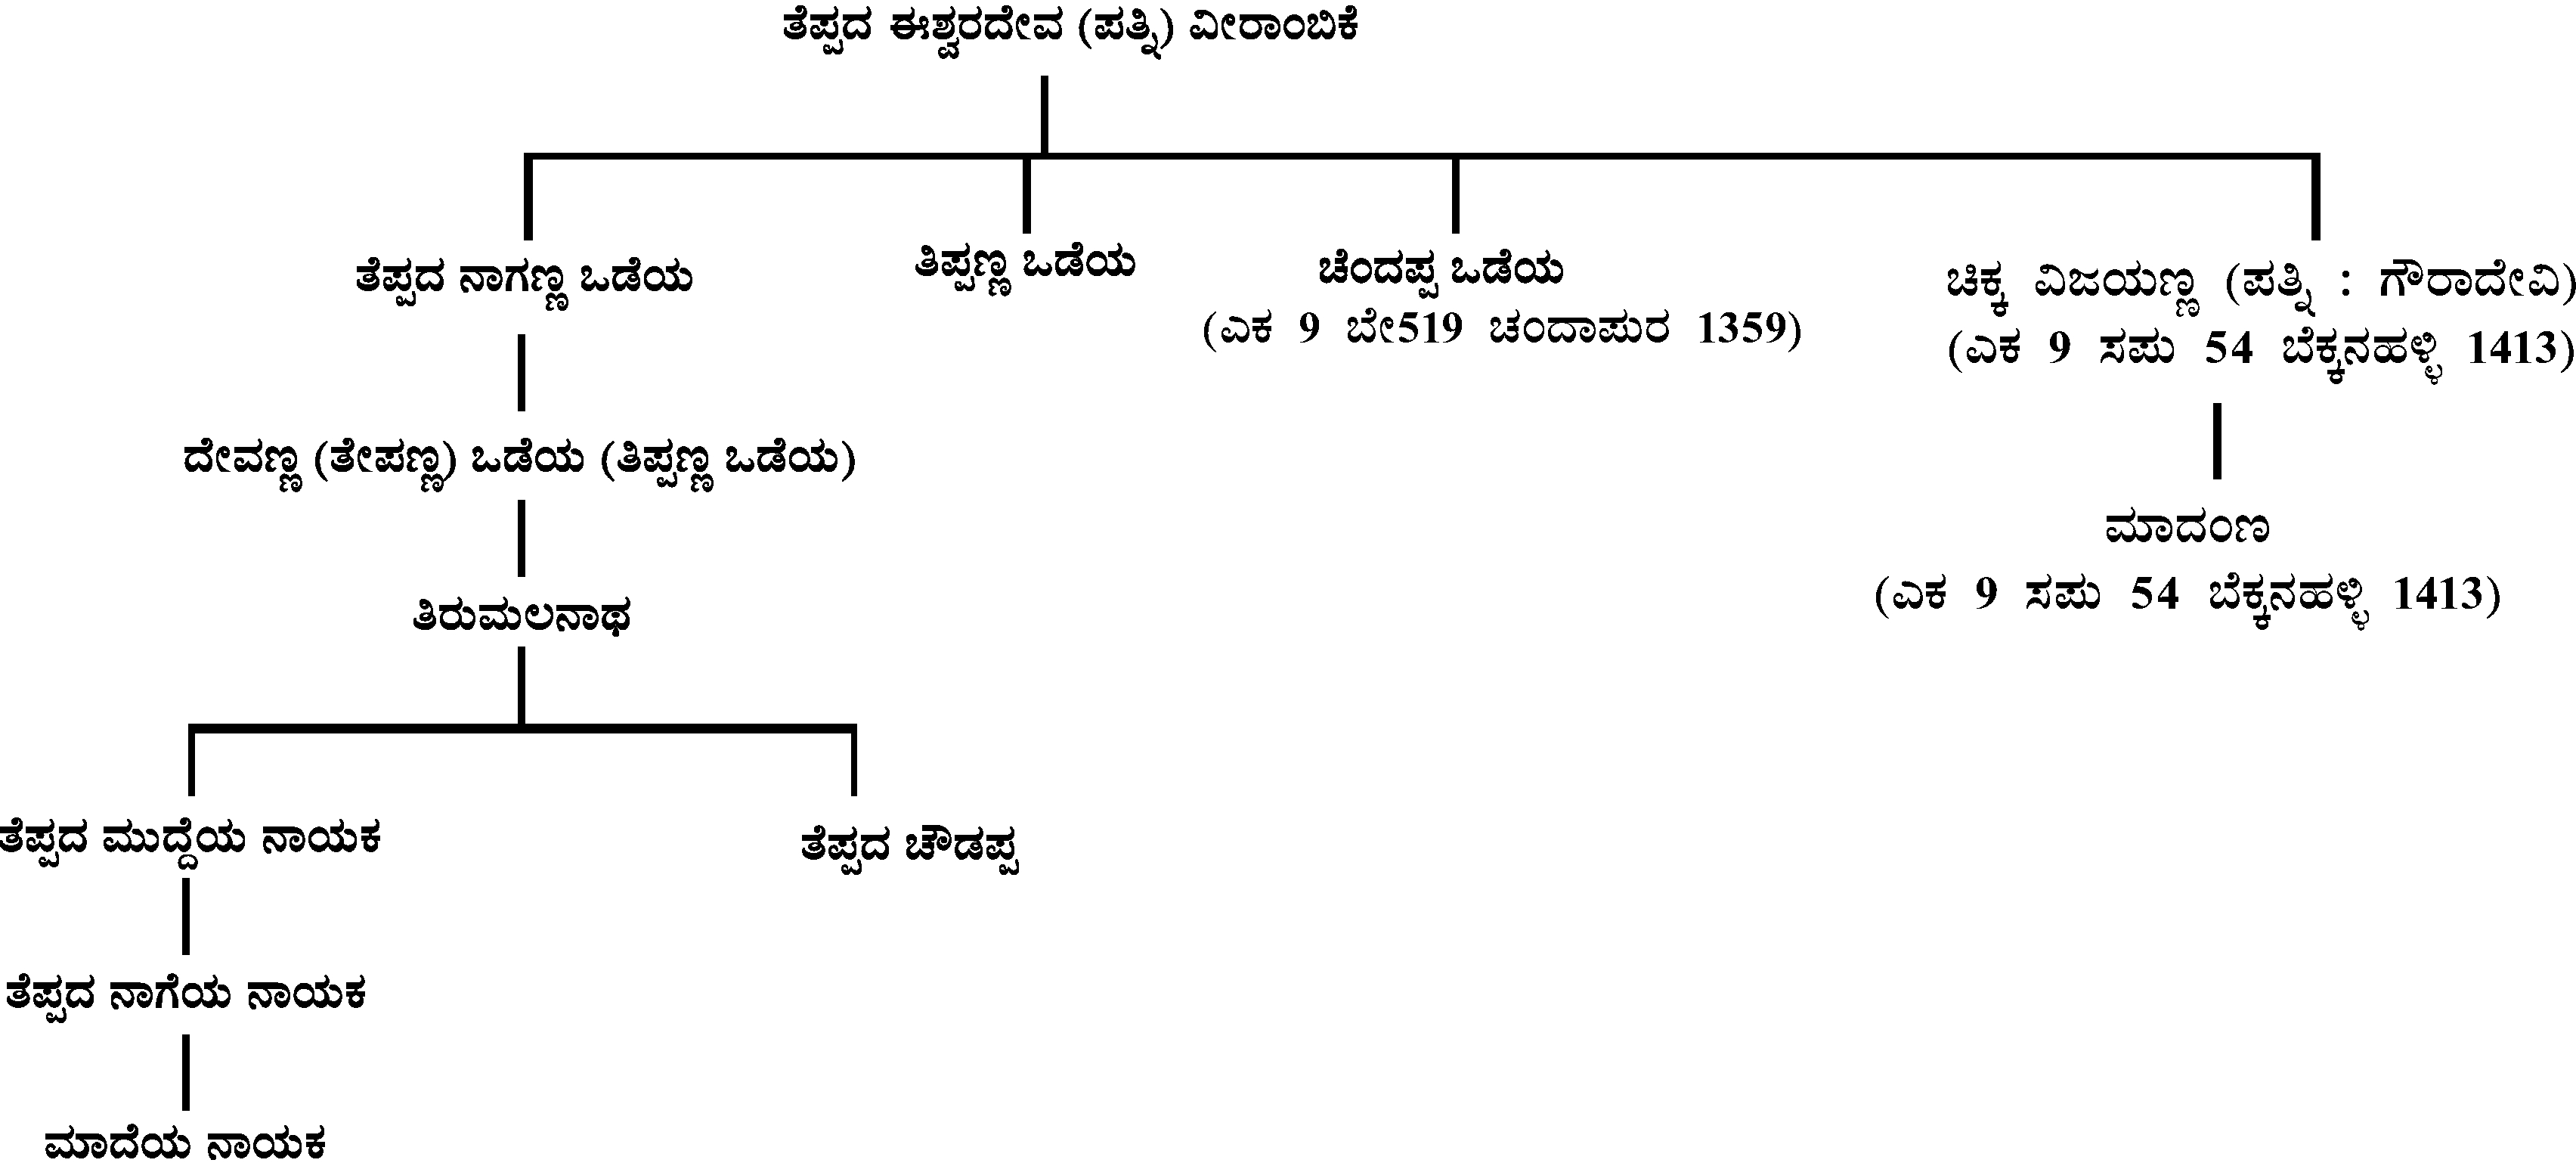
\includegraphics[scale=1.03]{images/chap3/chap3fig44.jpeg}
\end{figure}

\newpage

\textbf{ಮಹಾನಾಯಂಕಾಚಾರ್ಯ\index{ಮಹಾನಾಯಂಕಾಚಾರ್ಯ (ನಾಯಕಾಚಾರ್ಯ)} ಚಿಕ್ಕಅಲ್ಲಪ್ಪನಾಯಕ\index{ಚಿಕ್ಕ ಅಲ್ಲಪ್ಪನಾಯಕ} (1472):} ಸಾಳುವ ನರಸಿಂಗನ ಕಾಲದಲ್ಲಿ, ಶ‍್ರೀಮನ್ಮಹಾನಾಯಂಕಾ\-ಚಾರ್ಯ ಬಯಲಹುಲಿ\index{ಬಯಲಹುಲಿ} ಹಳಿಕಾಱ\index{ಹಳಿಕಾಱ (ಹಳ್ಳಿಕಾರ)} ಲಕ್ಕಣ್ಣನಾಯಕರ\index{ಲಕ್ಕಣ್ಣನಾಯಕರು} (ಲಚ್ಚಿಯನಾಯಕ) ಮಕ್ಕಳು ಚಿಕ್ಕಅಲ್ಲಪ್ಪ ನಾಯಕರು\index{ಚಿಕ್ಕ ಅಲ್ಲಪ್ಪನಾಯಕ}, ಶ‍್ರೀವೈಷ್ಣವರಾದ ಕೊನೆರಿ ಅಯ್ಯನವರಿಗೆ\index{ಕೊನೇರಿ ಅಯ್ಯ} ಗೋಪಿನಾಥದೇವರ\index{ಗೋಪಿನಾಥದೇವರು} ಸೇವೆಗಾಗಿ, ತನ್ನ ನಾಯಕತನಕ್ಕೆ ಸಲ್ಲುವ ದೇವಲಾಪುರದ\index{ದೇವಲಾಪುರ} ಹಿರಿಯಕೆರೆಯ ಕೆಳಗಣ ಅಡಕೆಮರದ ತೋಟವನ್ನು ದತ್ತಿಯಾಗಿ ಬಿಡುತ್ತಾನೆ.\endnote{ ಎಕ 7 ನಾಮಂ 157 ದೇವಲಾಪುರ 1472 ಜನವರಿ 26} ಇದೇ ಚಿಕ್ಕಅಲ್ಲಪ್ಪನಾಯಕನು ಮಹಾಮಂಡಳೇಶ್ವರ ಸಾಳುವ\break ನರಸಿಂಗನು ದೇವಲಾಪುರದ ಲಕ್ಷ್ಮೀಕಾಂತದೇವರ\index{ದೇವಲಾಪುರದ ಲಕ್ಷ್ಮೀಕಾಂತದೇವರು} ಸನ್ನಿಧಿಯಲ್ಲಿ ಸರ್ವ ಪ್ರಾಚೀನ ಕರ್ಮವಿಪಾಕ ದಾನವನ್ನು\index{ಪ್ರಾಚೀನ ಕರ್ಮವಿಪಾಕ ದಾನ} ಮಾಡಿದ ಸಂದರ್ಭದಲ್ಲಿ ಅವನಿಗೆ ಸಕಲ ಐಶ್ವರ್ಯ ಭಾಗ್ಯವಾಗಲಿ ಎಂದು ದೇವರಿಗೆ ದೀಪಮಾಲೆಯ ಕಂಬವನ್ನು ಬಾಗಿಲುವಾಡವನ್ನು ನಿಲ್ಲಿಸುತ್ತಾನೆ.\endnote{ ಎಕ 7 ನಾಮಂ 158 ದೇವಲಾಪುರ 1472 ಮೇ 22} ತೆಪ್ಪದ ಮನೆತನದ ನಂತರ ಚಿಕ್ಕ ಅಲ್ಲಪ್ಪ ನಾಯಕನು\index{ಚಿಕ್ಕ ಅಲ್ಲಪ್ಪನಾಯಕ} ದೇವಲಾಪುರವನ್ನು ಆಳುತ್ತಿದ್ದನೆಂದು ಊಹಿಸಬಹುದು.

\textbf{ಶಿಂಗಪ್ಪನಾಯಕ\index{ಶಿಂಗಪ್ಪನಾಯಕ} (15ನೇ ಶ.):} ಕರಬಸಾಣಿ\index{ಕರಬಸಾಣಿ} ಮಗ ಶಿಂಗಪ್ಪನಾಯಕನು, ವಿಷ್ಣುರಾಯ\index{ವಿಷ್ಣುರಾಯ} ಮಹಾರಾಯರಿಗೆ\index{ಮಹಾರಾಯ}\break (ಕೃಷ್ಣದೇವರಾಯ) ಧರ್ಮವಾಗಲೆಂದು, ಮೇಲುಕೋಟೆಯ\index{ಮೇಲುಕೋಟೆ} ನರಸಿಂಹದೇವರಿಗೆ ದತ್ತಿ ಬಿಡುತ್ತಾನೆ.\endnote{ ಎಕ 6 ಪಾಂಪು 109 ಕಟ್ಟೇನಹಳ್ಳಿ 15ನೇ ಶ.} ಕೃಷ್ಣದೇವರಾಯನ\index{ಕೃಷ್ಣದೇವರಾಯ} ಕೊಮಾರ ಸಿಂಗಪ್ಪನಾಯಕನು ಮಲ್ಲಿಕಾರ್ಜುನ\index{ಮಲ್ಲಿಕಾರ್ಜುನ}, ಭೀಮೇಶ್ವರ\index{ಭೀಮೇಶ್ವರ} ಮತ್ತು ವಿಘ್ನೇಶ್ವರ\index{ವಿಘ್ನೇಶ್ವರ} ದೇವರಿಗೆ ಸೇರಿದ ಭೂಮಿಗಳ ಮೇಲಿನ ತೆರಿಗೆಯನ್ನು ಮನ್ನಾ ಮಾಡಿದನೆಂದು ಹುಳಿಯಾರು ಶಾಸನದಲ್ಲಿ ಹೇಳಿದೆ.\endnote{ ಇಸಿ 12 ಚಿಕ್ಕನಾಯಕನಹಳ್ಳಿ 37 ಹುಳಿಯಾರು 1528} ಇವೆರಡೂ ಒಂದೇ ಕಾಲದ ಶಾಸನಗಳಾಗಿರುವುದರಿಂದ ಇವರಿಬ್ಬರೂ ಅಭಿನ್ನರಿರಬಹುದು.

\textbf{ಗೋಪಾಳದೇವ\index{ಗೋಪಾಳದೇವ} (1503):} ತುಳುವ ನರಸಣ್ಣ ನಾಯಕನು\index{ತುಳುವ (ನರಸ) ನರಸಣ್ಣ ನಾಯಕ (ವೀರನರಸಿಂಹ)} ಅಸ್ತಮಾನವಾದಾಗ ಅವರಿಗೆ ಧರ್ಮವಾಗಲೆಂದು,\break ಗೋಪಾಳದೇವನು ತನ್ನ ನಾಯಕತನಕ್ಕೆ ಸಲ್ಲುವ ಬಾಚಹಳ್ಳಿ ಸೀಮೆಯ\index{ಬಾಚಹಳ್ಳಿ ಸೀಮೆ/ಸ್ಥಳ}, ಯರಹಳ್ಳಿ ವೃತ್ತಿಯ ಬಿಕ್ಕಸಂದ್ರ\index{ಬಿಕಸಮುದ್ರ(ಬಿಕ್ಕಸಂದ್ರ)} ಗ್ರಾಮವನ್ನು ಬಾಚಿಹಳ್ಳಿಯ ವೀರನಾರಾಯಣದೇವರಿಗೆ\index{ಬಾಚಿಹಳ್ಳಿಯ ವೀರನಾರಾಯಣದೇವರು} ದತ್ತಿಯಾಗಿ ಬಿಡುತ್ತಾನೆ.\endnote{ ಎಕ 6 ಕೃಪೇ 63 ಸಂತೇಬಾಚಹಳ್ಳಿ 1503 ಡಿಸೆಂಬರ್​ 13} ಸಿಂದಘಟ್ಟ\index{ಸಿಂದಘಟ್ಟ} ಶಾಸನದ ರಂಗಯ್ಯ ನಾಯಕನು ಈತನ ವಂಶದವನಿರಬಹುದೆಂದು ಊಹಿಸಬಹುದು.

\textbf{ಕೆಂಪ ಬಯಿರರಸ ನಾಯಕ\index{ಕೆಂಪ ಬಯಿರರಸ ನಾಯಕ} (1507):} ಕಲಿಯ ಬಯಿರರಸ ನಾಯಕನ ಮಗ ಕೆಂಪ ಬಯಿರರಸ ನಾಯಕನು ಬಸರಾಳಿನ ಮಲ್ಲಿಕಾರ್ಜುನ ದೇವರಿಗೆ ಗದ್ದೆಯನ್ನು ದತ್ತಿ ಬಿಡುತ್ತಾನೆ.\endnote{ ಎಕ 7 ಮಂ 32 ಬಸರಾಳು 1507} ಇವನು ಪೂರ್ವೋಕ್ತ ಬಯಿರೆಯ ದಂಡನಾಯಕನ ವಂಶದವನಿರಬಹುದು.

\textbf{ಮಲೆಪ ನಾಯಕ\index{ಮಲೆಪ ನಾಯಕ}(1526):} ಕೃಷ್ಣದೇವರಾಯನ ಕಾಲದಲ್ಲಿ ಕಾಳಿಂಗರಾಮನಹಳ್ಳಿಯ (ಇಂದಿನ ನಾಗಮಂಗಲ ತಾ. ಕಾಳಿಂಗನಹಳ್ಳಿ) ನಾಯಕನಾಗಿದ್ದ ತಿಮ್ಮಯ್ಯನ ಮಗ ಮಲೆಪನಾಯಕನು ಕಾಳಿಂಗರಾಮನಹಳ್ಳಿಯ ತೆಂಕಳ(ಣ) ಭಾಗವನ್ನು ಮೇಲುಕೋಟೆಯ ಚೆಲುವಪಿಳ್ಳೆ ದೇವರ ಕೈಂಕರ್ಯಕ್ಕೆ ಮೇಲುಕೋಟೆಯ ಚೋಳಪ್ಪಯ್ಯನ ಹಸ್ತ ದತ್ತಿ ಬಿಡುತ್ತಾನೆ.\endnote{ ಎಕ 7 ನಾಮಂ 123 ಕಾಳಿಂಗನಹಳ್ಳಿ 1526}

\textbf{ಅಹೋಬಳರಾಜನ ಮಗ ವೆಂಕಟಾದ್ರಿ\index{ವೆಂಕಟಾದ್ರಿ ನಾಯಕ} (1528):} ಆಚರಾಜ ಅಹೋಬಳರಾಜನ\index{ಅಹೋಬಳರಾಜಯ್ಯ} ಮಗ ವೆಂಕಟಾದ್ರಿ ರಾಜನು\break ಕೃಷ್ಣದೇವರಾಯನ ಕಾಲದಲ್ಲಿ ನಾಯಕನಾಗಿ ಆಳುತ್ತಿದ್ದನೆಂದು ಹೇಳಬಹುದು. ರಾಜನಿಂದ ತನಗೆ ಸರ್ವಮಾನ್ಯವಾಗಿ ಬಂದ ಅಹೋಬಳಪುರವೆಂಬ ಪ್ರತಿನಾಮಧೇಯವುಳ್ಳ ಗ್ರಾಮವನ್ನು ರಾಮಾನುಜಕೂಟಕ್ಕೆ\index{ರಾಮಾನುಜಕೂಟ} ದತ್ತಿಬಿಟ್ಟನೆಂದು ಮೇಲುಕೋಟೆ\index{ಮೇಲುಕೋಟೆ} ಶಾಸನದಿಂದ ತಿಳಿದುಬರುತ್ತದೆ. ಈ ತ್ರುಟಿತ ಶಾಸನದಲ್ಲಿ ರಾಜನಹೆಸರು, ಗ್ರಾಮದ ಹೆಸರು ಹಾಗೂ ಇತರ ವಿವರಗಳು ಅಳಿಸಿಹೋಗಿವೆ.\endnote{ (ಎಕ 6 ಪಾಂಪು 162 ಮೇಲುಕೋಟೆ 1526)}

\textbf{ಅಹೋಬಲ ದೇವಗಳ ಮಕ್ಕಳು ಕೃಷ್ಣರಾಯ ನಾಯಕ\index{ಕೃಷ್ಣರಾಯ ನಾಯಕ}(1528):} ಕೃಷ್ಣಪ್ಪ ನಾಯಕನು, ತಾನು ಕಾಶ್ಯಪಗೋತ್ರದ, ಆಶ್ವಲಾಯನ ಸೂತ್ರದ, ಋಕ್​ಶಾಖೆಗೆ ಸೇರಿದವನೆಂದು, ಶ‍್ರೀರಂಗಪಟ್ಟಣದ ರಂಗನಾಥ\index{ಶ‍್ರೀರಂಗಪಟ್ಟಣದ ರಂಗನಾಥ} ದೇವರ ದಾಸಾನುದಾಸನೆಂದು\index{ದಾಸಾನುದಾಸ} ಹೇಳಿಕೊಂಡಿದ್ದಾನೆ. ದಂಡು ಅಹೋಬಲದೇವಗಳ\index{ದಂಡು ಅಹೋಬಲದೇವ} ಮಗ ಕೃಷ್ಣರಾಯನಾಯಕನು, ಕೃಷ್ಣದೇವರಾಯನು\index{ಕೃಷ್ಣದೇವರಾಯ} ತನ್ನ ನಾಯಕತನಕ್ಕೆ ದಯಪಾಲಿಸಿದ್ದ ಶ‍್ರೀರಂಗಪಟ್ಟಣಸೀಮೆಯ\index{ಶ‍್ರೀರಂಗಪಟ್ಟಣ ಸೀಮೆ} ಕುರುವಂಕನಾಡ\index{ಕುರುವಂಕ ನಾಡು} ಬೀರಸೆಟ್ಟಿ ಹಳ್ಳಿಯನ್ನು\index{ಬೀರಸೆಟ್ಟಿ ಹಳ್ಳಿ (ಬೀರಿ ಸೆಟ್ಟಿಹಳ್ಳಿ)},\endnote{ ಎಕ 6 ಶ‍್ರೀಪ 2 ಶ‍್ರೀರಂಗಪಟ್ಟಣ 1528 ಜನವರಿ 24} ಶ‍್ರೀರಂಗಪಟ್ಟಣ ಸೀಮೆಯ ಕಾಮೆಯನಾಯಕನಹಳ್ಳಿ\index{ಕಾಮೆಯನಾಯಕನಹಳ್ಳಿ}, ಸಿಂದಘಟ್ಟ ಸೀಮೆಯ\index{ಸಿಂದಘಟ್ಟ ಸೀಮೆ} ಗೊಲ್ಲರಚೆಟ್ಟನಹಳ್ಳಿಯ\index{ಗೊಲ್ಲರಚೆಟ್ಟನಹಳ್ಳಿ} ಸುಂಕಗಳನ್ನು,\endnote{ ಎಕ 6 ಪಾಂಪು 134 ಮೇಲುಕೋಟೆ ಜನವರಿ 28} ಕೃಷ್ಣದೇವರಾಯನಿಗೆ ಪುಣ್ಯವಾಗ\-ಬೇಕೆಂದು ದತ್ತಿಯಾಗಿ ಬಿಡುತ್ತಾನೆ. ಇದು ಕೃಷ್ಣದೇವರಾಯನ ಕೊನೆಯ ದಿನಗಳ ಶಾಸನವಾಗಿದ್ದು, ಈ ಕಾಲದಲ್ಲಿ ಸಿಂಹಾಸನಕ್ಕಾಗಿ ಕೃಷ್ಣದೇವರಾಯನ ಮಗನ ಕೊಲೆ ನಡೆದುದರ ಜೊತೆಗೆ, ಕೃಷ್ಣದೇವರಾಯನು ಖಾಯಿಲೆ ಬಿದ್ದಿದ್ದನೆಂದು ತಿಳಿದುಬರುತ್ತದೆ.\endnote{ ದೇಸಾಯಿ ಡಾ॥ ಪಿ.ಬಿ., ವಿಜಯನಗರ ಸಾಮ್ರಾಜ್ಯ, ಪುಟ 93-94}

ಅಚ್ಯುತರಾಯನ ಕಾಲದಲ್ಲಿ ವೆಂಕಟಾದ್ರಿನಾಯಕನು\index{ವೆಂಕಟಾದ್ರಿನಾಯಕ} ಪುರದ ಮಾಗಣಿಗೆ\index{ಪುರದ ಮಾಗಣಿ} ಸಲ್ಲುವ, ದೇವಲಾಪುರ ಸ್ಥಳದ\index{ದೇವಲಾಪುರ ಸ್ಥಳ} ದಾನದ \hbox{ಅಂಮನ} ಪುರದ\index{ದಾನದ ಅಂಮನ ಪುರ} ಸುಂಕವನ್ನು ಮಲ್ಲುನಾಯಕನಹಳ್ಳಿ\index{ಮಲ (ಮಲ್ಲು-ಮಲು) ನಾಯಕನಹಳ್ಳಿ} ವೆಂಕಟರಮಣ ದೇವರಿಗೆ\index{ವೆಂಕಟರಮಣ ದೇವರು} ಮಾನ್ಯವಾಗಿ ಬಿಡುತ್ತಾನೆ.\endnote{ ಎಕ 7 ನಾಮಂ 142 ದೇವರಹಳ್ಳಿ 1537}

\vskip 3pt

\textbf{ಮಹಾನಾಯಕಾಚಾರ್ಯ\index{ಮಹಾನಾಯಂಕಾಚಾರ್ಯ (ನಾಯಕಾಚಾರ್ಯ)} ಗಿರಿಯಣ್ಣನಾಯಕ\index{ಗಿರಿಯಣ್ಣನಾಯಕ} (1529):} ಶ‍್ರೀಮನ್​ ಮಹಾನಾಯಕಾಚಾರ್ಯ ಬಯಲಹುಲಿ ಅವರೆಗೆರೆಯ ಗಿರಿಯಣ್ಣನಾಯಕರ ಮಕ್ಕಳು ವಿರುಪಣ್ಣ ನಾಯಕರು, ಲಕ್ಷ್ಮೀದೇವರ ಗುಡಿಯನ್ನು ಕಟ್ಟುವುದಕ್ಕಾಗಿ ಸುಂಕದ ಗದ್ಯಾಣ 14 ವರಹವನ್ನು, ದೇವರ ಹಳ್ಳಿಯ ತಪಸೀರಾಯನ\index{ದೇವರ ಹಳ್ಳಿಯ ತಪಸೀರಾಯ} ಭಂಡಾರಕ್ಕೆ ದತ್ತಿಯಾಗಿ ಕೊಡುತ್ತಾನೆ.\endnote{ ಎಕ 7 ನಾಮಂ 143 ಕೊಡಗಹಳ್ಳಿ 1529}

\vskip 3pt

\textbf{ರಾಯಣ್ಣ ನಾಯಕ\index{ರಾಯಣ್ಣ ನಾಯಕ} ಮತ್ತು ತಿಪ್ಪಣ್ಣ ನಾಯಕ\index{ತಿಪ್ಪಣ್ಣ ನಾಯಕ} (1530):} ಅಚ್ಯುತರಾಯನು ವಿದ್ಯಾನಗರಿಯ\index{ವಿದ್ಯಾನಗರಿ} ಸಿಂಹಾಸನದಿಂದ ಆಳುತ್ತಿದ್ದಾಗ, ರಾಯಣ\-ನಾಯಕನು ಅವನಿಗೆ ಪುಣ್ಯವಾಗಬೇಕೆಂದು, ಮಾಯಣನಪುರ\index{ಮಾಯಣನಪುರ} ಗ್ರಾಮವನ್ನು ತಲಕಾಡು ಕೀರ್ತಿ\-ನಾರಾಯಣದೇವರಿಗೆ ದತ್ತಿಬಿಟ್ಟ\-ನೆಂದು ಕೊಡಗಹಳ್ಳಿ ಶಾಸನದಿಂದ ತಿಳಿದು ಬರುತ್ತದೆ.\endnote{ ಎಕ 7 ಮವ 108 ಕೊಡಗಹಳ್ಳಿ 1530} ಇದೇ ದಿನ \textbf{ತಿಪ್ಪಣ್ಣನಾಯಕನೆಂಬುವನೂ} ಕೂಡಾ ಅಚ್ಯುತರಾಯರಿಗೆ ಪುಣ್ಯವಾಗಬೇಕೆಂದು, ಮಾರೆಹಳ್ಳಿ ಪಟ್ಟಣದ\index{ಮಾರೆಹಳ್ಳಿ ಪಟ್ಟಣ} ಬಳಿಯ (ಕುಂದೂರು)\index{ಕುಂದೂರು} ಮೂಲಸ್ಥಾನದೇವರಿಗೆ ಗದ್ದೆಯನ್ನು ಕೃಷ್ಣವೇಣಿ\index{ಕೃಷ್ಣವೇಣಿ} ತೀರದಲ್ಲಿ ದತ್ತಿಬಿಡುತ್ತಾನೆ.\endnote{ ಎಕ 7 ಮವ 78 ಮಾರೆಹಳ್ಳಿ 1530} ಈ ಶಾಸನಗಳು 1530 ಅಕ್ಟೋಬರ್​ 6ರಂದು ಹೊರಟಿವೆ. ಬಹುಶಃ ಈ ತಾರೀಖಿನಂದು ಅಚ್ಯುತರಾಯನು ಅನೇಕ ಅಡೆತಡೆಗಳನ್ನು ನಿವಾರಿಸಿಕೊಂಡು ಪಟ್ಟಕ್ಕೆ ಬಂದಿರಬಹುದು.

\vskip 3pt

\textbf{ಕದರೆಯನಾಯಕ\index{ಕದರೆಯನಾಯಕ} (1531):} ಬಳಗುಂದಿಯ ತಿಪ್ಪಯ್ಯನ ಮಗ ಕದರೆಯನಾಯಕನು ಕೆರೆಯನ್ನು ಕಟ್ಟಿಸಿದನೆಂದು ನಾಗಮಂಗಲ ತಾಲ್ಲೂಕು ಶಿವನಹಳ್ಳಿ ಶಾಸನದಿಂದ ತಿಳಿದುಬರುತ್ತದೆ.\endnote{ ಎಕ 7 ನಾಮಂ 21 ಶಿವನಹಳ್ಳಿ 1531} ಈ ಕಡೆಯಲ್ಲಿ ಜನರು ಕದರಪ್ಪ ಎಂಬ ಹೆಸರನ್ನು ಇಟ್ಟುಕೊಳ್ಳುತ್ತಿದ್ದರು.

\vskip 3pt

\textbf{ರಂಗಯ್ಯನಾಯಕ\index{ರಂಗಯ್ಯ ನಾಯಕ}(1537):} ಸಿಂಧಘಟ್ಟದ ಒಳಕೇರಿಯಲ್ಲಿ\index{ಸಿಂಧಘಟ್ಟದ ಒಳಕೇರಿ} ಬಾಬುಸೆಟ್ಟಿಯು\index{ಬಾಬುಸೆಟ್ಟಿ} ಕಟ್ಟಿಸಿದ ಕಲ್ಲುಮಸೀದಿಗೆ\index{ಕಲ್ಲುಮಸೀದಿ}, ರಂಗಯ್ಯ\-ನಾಯಕನು ಶಿವಪುರ\index{ಶಿವಪುರ} ಗ್ರಾಮವನ್ನು ಸರ್ವಮಾನ್ಯವಾಗಿ ಬಿಡುತ್ತಾನೆ.\endnote{ ಎಕ 6 ಕೃಪೇ 92 1537} ಇವನು ಸಿಂದಘಟ್ಟ ಸೀಮೆಯ ನಾಯಕನಾಗಿರಬಹುದು. ಸಿಂದಘಟ್ಟಕ್ಕೆ ಸಮೀಪದ ನಾರಾಯಣಗಿರಿದುರ್ಗ\index{ನಾರಾಯಣಗಿರಿ ದುರ್ಗ} ಬೆಟ್ಟದ ಮೇಲೆ ಏಳು ಸುತ್ತಿನ ಕೋಟೆಯ ದುರ್ಗವನ್ನು ಕಟ್ಟಿಕೊಂಡು ಆಳುತ್ತಿದ್ದನೆಂದು ತೋರುತ್ತದೆ. ಬೆಟ್ಟದಮೇಲೆ ಕೈವಲ್ಯೇಶ್ವರ ದೇವಾಲಯ\index{ಕೈವಲ್ಯೇಶ್ವರ ದೇವಾಲಯ}, ಅಮ್ಮನವರಗುಡಿ, ಕೊಳಗಳು, ಮದ್ದಿನಮನೆ, ಇವೆ. ದೇವಾಲಯದ ಗೋಡೆಯ ಮೇಲೆ ರಂಗಯ್ಯನ ಶಾಸನವಿದ್ದು ಅದು ತ್ರುಟಿತವಾಗಿದೆ. ರಾಯಸಮುದ್ರ\index{ರಾಯಸಮುದ್ರ} ಇವನ ಪಾಳೆಯಪಟ್ಟೆಂದು ಹೇಳಿದೆ.\endnote{ ಪುರುಷೋತ್ತಮ, ಸಿ.ಜಿ., ಸಿಂಧಘಟ್ಟದ ಶಾಸನ, ಇಕ್ಷುಕಾವೇರಿ, ಪುಟ 112} ಇವನೂ ಸಂತೇಬಾಚಹಳ್ಳಿಯ ಕ್ರಿ.ಶ.1553ರ ಶಾಸನೋಕ್ತ ಅಹೋಬಲದೇವರಾಜಯ್ಯ\index{ಅಹುಬಳದೇವರಾಜಯ್ಯದೇವ ಚೋಳ ಮಹಾ ಅರಸ} ದೇವ ಚೋಳ ಮಹಾಅರಸುಗಳ ಕಾರ್ಯಕೆ ಕರ್ತನಾದ ರಂಗಪಯ್ಯನೂ ಅಭಿನ್ನರೆಂದು ಹೇಳಬಹುದು.

\vskip 3pt

\textbf{ಚನ್ನರಾಜ\index{ಚನ್ನರಾಜ}, ತಿಮ್ಮಪ್ಪನಾಯಕ\index{ತಿಮ್ಮಪ್ಪನಾಯಕ}, ಕದಪನಾಯಕ\index{ಕದಪನಾಯಕ}, ತಿರುಣನಾಯಕ\index{ತಿರುಣನಾಯಕ} (1544):} ಸದಾಶಿವಮಹಾರಾಯನ ಕಾಲದಲ್ಲಿ, ಚಂನರಾಜ, ತಿಂಮಪನಾಯಕ, ಕದಪನಾಯಕ ಮತ್ತು ತಿರುಣನಾಯಕ ಇವರುಗಳು ನಾಗಮಂಗಲ ಅಗ್ರಹಾರವನ್ನು ತಮ್ಮ ಸ್ವಾಮಿಯ (ಸದಾಶಿವರಾಯನ) ನಿರೂಪದಂತೆ ಪುರದಾನವಾಗಿ ನೀಡುತ್ತಾರೆ.\endnote{ ಎಕ 7 ನಾಮಂ 6 ನಾಗಮಂಗಲ 1544} ಇವರು ನಾಗಮಂಗಲವನ್ನು ಆಳುತ್ತಿದ್ದ ನಾಯಕರಿದ್ದು ಸಹೋದರರಾಗಿರಬಹುದು. ಸುಮಾರು 1630ರಲ್ಲಿ ನಾಗಮಂಗಲವನ್ನು ಆಳುತ್ತಿದ್ದು, ಐದನೆಯ ಚಾಮರಾಜ ಒಡೆಯರಿಂದ ಸೋಲಿಸಲ್ಪಟ್ಟ ಚನ್ನಯ್ಯನು\index{ಚನ್ನಯ್ಯ} ಇವರ ವಂಶದವನೇ ಎಂದು ಊಹಿಸಬಹುದು.\endnote{ \engfoot{Sathyanarayana, Dr. A., History of the Wodeyars of Mysore, pp.36, 44}}

\textbf{ಕುಂಚಿಕೊಂಡ ಭೂಪಾಲನ\index{ಕುಂಚಿಕೊಂಡಭೂಪಾಲ} ಮಗ ವೆಂಕಟಾದ್ರಿನಾಯಕ\index{ವೆಂಕಟಾದ್ರಿನಾಯಕ} (1545):} ವೆಂಕಟಾದ್ರಿನಾಯಕನು ಸದಾಶಿವರಾಯನ ಕಾಲದಲ್ಲಿ ಪೆನುಗೊಂಡೆ ರಾಜ್ಯದ\index{ಪೆನುಗೊಂಡೆ (ರಾಜ್ಯ- ಮಹಾರಾಜ್ಯ)}, ಹೊಯ್ಸಳ ನಾಡಿನ\index{ಹೊಯ್ಸಳ ನಾಡು} ಬೇಲೂರು ಸೀಮೆಯನ್ನು\index{ಬೇಲೂರು ಸೀಮೆ}(ಇಂದಿನ ನಾಗಮಂಗಲ ತಾಲ್ಲೂಕಿನ ಬೆಳ್ಳೂರು) ಆಳುತ್ತಿದ್ದನು. ಹೊನ್ನೇನಹಳ್ಳಿ\index{ಹೊನ್ನೇನಹಳ್ಳಿ} ತಾಮ್ರಶಾಸನವು ಈತನನ್ನು ಬಹುವಾಗಿ ಸ್ತುತಿಸಿದೆ. \textbf{“ಚತುರ್ಥಗೋತ್ರ ಕಲಶ ಸಿಂಧು ಸುಧಾನಿಧೇಃ। ಸ್ವಾಮಿಕಾರ್ಯ ಧುರೀಣಸ್ಯ ಸ್ವಾಧೀನನಯಸಂಪದಃ। ವಿನಯಸ್ಯೇವ ಮೂರ್ತಸ್ಯ ವಿಶ್ವಾಸಾವಾಸವೇಶ್ಮನಃ। ಸರ್ವ್ವಧರ್ಮ್ಮರಹಸ್ಯಸ್ಯ ಸರ್ವಭೂತಾನುಕಂಪಿನಃ। ಮೃಷ್ಟಾಂನದಾನ ಸಾಂತತ್ಯ ತುಷ್ಟಾಶೇಷದ್ವಿಜನ್ಮನಃ। ಧರ್ಮ್ಮಶೀಲಾಕ್ಕಮಾಗರ್ಭಶುಕ್ತಿಮುಕ್ತಾಫಲಾ ತ್ಮನಃ। ಶ‍್ರೀ ಕುಂಚಿಕೊಂಡ ಭೂಪಾಲ ಚಿರಪುಣ್ಯ ಫಲಾಕೃತೇಃ। ವೇಂಕಟಾದ್ರೀಶ ಪಾದಾಬ್ಜ ಕೃಕಟಾಯಿತಚೇತಸಃ। ಚವರಂ\general{\break } ವೆಂಕಟಾದ್ರೀಶನಾಯಕಸ್ಯ ನಯೋಂನತೇಃ।”} ಚತುರ್ಥಗೋತ್ರದ ಕುಂಚಿಕೊಂಡ ಭೂಪಾಲ ಮತ್ತು ಅಕ್ಕಮಾ ಇವರ ಮಗನಾದ ವೆಂಕಟಾದ್ರಿನಾಯಕನು ಸದಾಶಿವರಾಯನಿಗೆ ವಿಜ್ಞಾಪನೆಯನ್ನು ಮಾಡಿಕೊಂಡು ಹೊಂನಯನಹಳ್ಳಿಯನ್ನು ವೆಂಕಟಾದ್ರಿಸಮುದ್ರ\-ವೆಂಬ\index{ವೆಂಕಟಾದ್ರಿಸಮುದ್ರ} ಅಗ್ರಹಾರವನ್ನಾಗಿ ಮಾಡಿ ಬ್ರಾಹ್ಮಣರಿಗೆ ದತ್ತಿಹಾಕಿಕೊಡುತ್ತಾನೆ.\endnote{ ಎಕ 7 ನಾಮಂ 107 ಹೊನ್ನೇನಹಳ್ಳಿ 1545 ಜೂನ್​ 24} ಈತನು ಬೇಲೂರಿನ ವೆಂಕಟಾದ್ರಿನಾಯಕನಿಂದ ಭಿನ್ನನು.

\newpage

\textbf{ೞೋ(ಳೋ)ಡವನಾಯಕ\index{ೞೋ(ಳೋ)ಡವನಾಯಕ} ಮತ್ತು ಕೆಂಚಪನಾಯಕ\index{ಕೆಂಚಪನಾಯಕ} (1560): }ಬಲೆಯನಾಯಕರ ಮಕ್ಕಳು ೞೋಡವನಾಯಕರು,\break ಲಖಪನಾಯಕರ ಮಕ್ಕಳು ಕೆಂಚಪನಾಯಕರು ತಮ್ಮ ಒಡೆಯ ವಿರುಪರಾಜ\index{ವಿರುಪರಾಜ} ಒಡೆಯನಿಗೆ ಪುಣ್ಯವಾಗಬೇಕೆಂದು, ಕಹಿನ ತಿರುಮಲ ದೇವರಿಗೆ\index{ಕಹಿನ ತಿರುಮಲ ದೇವರು}, ಬೆಳ್ಳೂರು ಸೀಮೆಯ\index{ಬೆಲೂರು (ಬೆಲ್ಲೂರು) (ಬೆಳ್ಳೂರು) ಸೀಮೆ} ಒಂದು ಗ್ರಾಮವನ್ನು (ಕದಬಳ್ಳಿ\index{ಕದಬಳ್ಳಿ} ಇರಬಹುದು) ಧಾರೆಯೆರೆದುಕೊಟ್ಟರೆಂದು ಕದಬಳ್ಳಿ ಶಾಸನದಲ್ಲಿ ಹೇಳಿದೆ.\endnote{ ಎಕ 7 ನಾಮಂ 71 ಕದಬಳ್ಳಿ 1560} ಈ ಕಾಲದಲ್ಲಿ ಸದಾಶಿವರಾಯನು ಆಳುತ್ತಿದ್ದನು. ಕಹಿನ ತಿರುಮಲ ದೇವರನ್ನು ಈಗ ಕಾವೇಟಿರಂಗ\index{ಕಾವೇಟಿರಂಗ} ಎನ್ನುತ್ತಾರೆ.\endnote{ ಇವರು ಕದಬಹಳ್ಳಿ ಸೀಮೆಯನ್ನು ಆಳುತ್ತಿದ್ದರೆಂದು ಹೇಳಬಹುದು.}

\textbf{ಸುರಗಿಯ ದೇವಪ್ಪನಾಯಕ\index{ಸುರಗಿಯ ದೇವಪ್ಪನಾಯಕ} (1640):} ಸದಾಶಿವರಾಯನ ಕಾಲದಲ್ಲಿ ಸುರಗಿಯ ದೇವಪ್ಪನಾಯಕನು, ತನ್ನ ನಾಯಕ\-ತನಕ್ಕೆ ಸಲ್ಲುವ ದೇವಲಾಪುರದ ಸೀಮಾಸಂಬಂಧಿ ಗ್ರಾಮವನ್ನು (ಕುಡುಗುಬಾಳು\index{ಕುಡುಗುಬಾಳು}), ಕುಡಗಬಾಳ ರಾಮಲಿಂಗದೇವರಿಗೆ\index{ರಾಮಲಿಂಗದೇವರು} ದತ್ತಿಬಿಡುತ್ತಾನೆ.\endnote{ ಎಕ 7 ನಾಮಂ 165 ಕುಡುಗಬಾಳು 1640} ಇವನು ವಿಷ್ಣುವರ್ಧನನ ಮಹಾಪ್ರಧಾನ ದಂಡನಾಯಕನಾಗಿದ್ದ, ಸುರಗಿಯ ನಾಗಯ್ಯನ\index{ಸುರಿಗೆಯ (ಸುರಗಿಯ) ನಾಗಯ್ಯ (ನಾಗಿದೇವ, ನಾಗಣ್ಣ)} ವಂಶದವನೆಂದು ಊಹಿಸಬಹುದು.

\section*{ಸ್ಥಳೀಯ ಅಧಿಕಾರವರ್ಗದವರು}

\textbf{ಗಾವುಂಡರು\index{ಗಾವುಂಡರು}/ ಗವುಡುಗಳು\index{ಗವುಡುಗಳು}/ ಪ್ರಭುಗಾವುಂಡರು\index{ಪ್ರಭು ಗಾವುಂಡ (ಗಾವುಂಡರು) (ಗವುಡುಗಳು)}/ಪ್ರಜೆಗಾವುಂಡರು\index{ಪ್ರಜೆಗಾವುಂಡರು}}

ವಿಜಯನಗರ ಕಾಲದ ಸ್ಥಳೀಯ ಸರ್ಕಾರದಲ್ಲಿ, “ಗಾವುಂಡರು ಗ್ರಾಮ ಅಥವಾ ಹಳ್ಳಿಯ ಆಡಳಿತದ ಮುಖ್ಯಸ್ಥರಾಗಿರು\-ತ್ತಿದ್ದರು. ಸೇನಬೋವ ಅಥವಾ ಕುಲಕರಣಿಗಳು ಗ್ರಾಮದ ಲೆಕ್ಕಪತ್ರಗಳನ್ನು ನಿರ್ವಹಿಸುತ್ತಿದ್ದರು. ಇವರ ಕೈಕೆಳಗೆ ಸೇವಕರಾಗಿ ಆಯಗಾರರು, ತಳಾರರು, ಬಾರಿಕರು ಮತ್ತು ತೋಟಿ ಅಥವಾ ತೋಟಿಗರು ಇರುತ್ತಿದ್ದರು” ಎಂದು ವೆಂಕಟರತ್ನಂ ಅವರುಹೇಳಿದ್ದಾರೆ.\endnote{ \engfoot{Venkataratnam, Dr.A.V. Local Government in the Vijayanagara Empire, pp.24}} ಪ್ರಜೆ ಎಂಬುದು ಗ್ರಾಮ ನಿವಾಸಿಗಳ ಪ್ರತಿನಿಧಿಗಳನ್ನು ಒಳಗೊಂಡ ಒಂದು ಸಂಸ್ಥೆಯಾಗಿತ್ತು, ಈ ಸಂಸ್ಥೆಯ ಮುಖ್ಯಸ್ಥರಾಗಿ ಗ್ರಾಮ ಗಾಮುಂಡ, ಪ್ರಜೆಗಳು ಇರುತ್ತಿದ್ದರು.\endnote{ ಅದೇ, ಪುಟ 25-27} ಒಂದು ಹಳ್ಳಿಗೆ ಮುಖ್ಯಸ್ಥರಾಗಿ ಗಾವುಂಡರು ಅಥವಾ ಪ್ರಭುಗಳು ಇದ್ದರೆ, ಹಳ್ಳಿಗಳ ಗುಂಪು ಅಥವಾ ನಾಡು ಅಥವಾ ಕಂಪಣದ ಮುಖ್ಯಸ್ಥರಾಗಿ ನಾಡಗಾವುಂಡರು, ನಾಡಪ್ರಭುಗಳು ಇರುತ್ತಿದ್ದರು. ನಾಡು ಎಂಬುದು ಇನ್ನೊಂದು ರೀತಿಯ ಸ್ಥಳೀಯ ಸಭೆಯಾಗಿತ್ತು ಎಂದು ಅವರು ಹೇಳುತ್ತಾರೆ.\endnote{ ಅದೇ, ಪುಟ 76-77} ಗವುಡು ಅಥವಾ ಗಾವುಂಡರಿಗೆ ಕೊಡುಗೆ, ಉಂಬಳಿ ಅಥವಾ ಮಾನ್ಯವನ್ನು ನೀಡಲಾಗುತ್ತಿತ್ತು. ಇದನ್ನು ಗೌಡಿಕೆ ಉಂಬಳಿ ಎಂದು ಕರೆಯಲಾಗತ್ತಿತ್ತು. ಗಾವುಂಡರ ಹುದ್ದೆಯು ವಂಶಪಾರಂಪರ್ಯವಾಗಿದ್ದರೂ, ವಿಜಯನಗರ ಮತ್ತು ನಂತರದ ಕಾಲದಲ್ಲಿ ಗೌಡರನ್ನು ರಾಜರು ನೇಮಿಸುತ್ತಿದ್ದರೆಂದು ತಿಳಿದುಬರುತ್ತದೆ. ಹಿರಿಯೂರು ತಾಲ್ಲೂಕಿನ ಸೂಗೂರಿನ ಕ್ರಿ.ಶ.1547ರ ಶಾಸನದಲ್ಲಿ ಹರತಿ ಐಮಂಗಳ ತಿಪ್ಪಳಿನಾಯಕನು ಸೂಗುರು ದೊಡ್ಡದ್ಯಾಮಗೌಡನಿಗೆ ಸದರಿ ಗ್ರಾಮದ ಸ್ಥಳದ ಗವುಡಿಕೆಗೆ ನೇಮಿಸಿ ನಿರೂಪ ಹೊರಡಿಸಿದನೆಂದೂ, ಇದಕ್ಕೆ ಆ ಊರಿನ ಹನ್ನೆರಡು ಆಯಗಾರರು ಸಾಕ್ಷಿಯಾಗಿದ್ದರೆಂದು ತಿಳಿದುಬರುತ್ತದೆ.\endnote{ ಸೂರ್ಯನಾಥ ಕಾಮತ್​, ಡಾ॥, ಒಕ್ಕಲುತನ ಮತ್ತು ಒಕ್ಕಲಿಗರು: ಇತಿಹಾಸ ಅನ್ವೇಷಣೆ, ಪುಟ 128-29}

ಶ‍್ರೀರಂಗಪಟ್ಟಣ ತಾಲ್ಲೂಕು ಬಸ್ತಿಹಳ್ಳಿ ಶಾಸನವು, ಕೂರಿಗಿಹಳ್ಳಿಯ ಪ್ರಭುಗಳ\index{ಕೂರಿಗಿಹಳ್ಳಿಯ ಪ್ರಭುಗಳು} ವರ್ಣನೆಯನ್ನು ಅವರು ಹೊಂದಿದ್ದ ಸ್ಥಾನಮಾನ\-ಗಳನ್ನು ಸೂಚಿಸುತ್ತದೆ. \textbf{“ಕೂರಿಗಿಹಳ್ಳಿಯ ಪ್ರಭುಗಳು ಗಉಡುಕುಲತಿಲಕರುಂ\index{ಗಉಡುಕುಲತಿಲಕರು} ಮಱೆವೊಕ್ಕರಕಾವರುಂ ಶಿಥಿಲ\-ಬೆಂಕೊಂಬರುಂ ಸತ್ತ್ಯದಲಿ ಕರ್ನ್ನರುಂಮಪ ಕೇತಗಉಡ ರಾಮಗಉಡ\index{ರಾಮಗಉಡ} ಸಂಬುವಗಉಡ\index{ಸಂಬುವಗಉಡ} ಮಾದಿಗಉಡ\index{ಮಾದಿಗಉಡ (ಗವುಡ - ಗೌಡ)} ಮೊದಲಾದ ಸಮಸ್ತ ಗಉಡುಗಳು”} ಬಸದಿಯನ್ನು ಕಟ್ಟಿಸಿ ಪಾರ್ಶ್ವದೇವರ\index{ಪಾರ್ಶ್ವದೇವರು} ಅಮೃತಪಡಿಗೆ ಗದ್ದೆ ಬೆದ್ದಲುಗಳನ್ನು ದತ್ತಿ ಬಿಡುತ್ತಾರೆ.\endnote{ ಎಕ 6 ಶ‍್ರೀಪ 74 ಬಸ್ತೀಪುರ 1422} ಈ ಶಾಸನದಲ್ಲಿ ಯಾವುದೇ ರಾಜ ಅಥವಾ ಅಧಿಕಾರಿಯ ಹೆಸರಿಲ್ಲ. ನೇರವಾಗಿ ಗೌಡರೇ ಈ ಶಾಸನವನ್ನು ಹಾಕಿಸಿರುವುದು ವಿಶೇಷವಾಗಿದೆ. \hbox{ಅರಲವನ} ಹಳ್ಳಿಯ ಕೀರ್ತಿದೇವ ಅರಸನ ಮಕ್ಕಳು, ತಮ್ಮ ಗವುಡು ಮುಸುಕಮಾದೆಗೊಂಡನ\index{ಮುಸುಕಮಾದೆಗೊಂಡ (ಮಾದೇಗೌಡ)} ಮಗ ಚವುಡೆಗೊಂಡನಿಗೆ ಕೊಡುಗೆಯಾಗಿ ಗದ್ದೆಯನ್ನು ನೀಡುತ್ತಾರೆ.\endnote{ ಎಕ 7 ಮ 95 ಅರುವನಹಳ್ಳಿ 1345} ಕೀರ್ತಿದೇವನು ಅರುವನಹಳ್ಳಿಯ ಭಟ್ಟರ ಬಾಚಿಯಪ್ಪನ ತಂದೆ.

ಚಂದಹಳ್ಳಿಯನ್ನು ಪಟ್ಟಣವನ್ನಾಗಿ ಮಾಡಲು ಚಂದಹಳ್ಳಿಯ ಮಾಚಗೌಂಡ, ಮಂಚೇಗೌಂಡನ ಮಗ ಚಾವಗೌಂಡ, ಮಾರಗೌಂಡ, ಮೊದಲಾದ ಸಮಸ್ತ ಪ್ರಜೆಗಗೌಂಡಗಳು\index{ಸಮಸ್ತ ಪ್ರಜೆಗವುಡುಗಳು (ಗಾವುಂಡುಗಳು)}, ಪಟ್ಟಣಸ್ವಾಮಿಗಳಿಗೆ\index{ಪಟ್ಟಣಸ್ವಾಮಿ} ಶಾಸನ ಹಾಕಿಕೊಡುತ್ತಾರೆ.\endnote{ ಎಕ 7 ಮವ 81 ಚಂದಹಳ್ಳಿ 14ನೇ ಶ.} ಅರುಹನಹಳ್ಳಿಯ ಕೀರ್ತಿಯರಸನ ಮಕ್ಕಳು ಸಮಸ್ತ ಗವುಡುಪ್ರಜೆಗಳನ್ನು\index{ಸಮಸ್ತ (ಗೌಡು - ಗವುಡು) ಪ್ರಜೆಗಳು} ಮುಂದಿಟ್ಟುಕೊಂಡು, ಸಮಸ್ತ ಆಸ್ತಿಯನ್ನು ವಿಭಾಗ ಮಾಡಿಕೊಳ್ಳುತ್ತಾರೆ. ಇದಕ್ಕೆ ಸಾಕ್ಷಿಗಳಾಗಿ ಮಡಿಯನಹಳ್ಳಿಯ\index{ಮಡಿಯನಹಳ್ಳಿ} (ಇಂದಿನ ಮಡೇನಹಳ್ಳಿ) ಮಾಯಿಗೌಡನ ಮಕ್ಕಳು ಸಾವಂತಗೌಡ, ಹೂಲಿಕೆರೆಯ ಜಗ್ಗಗವುಡನ ಮಕ್ಕಳು ಮಂಚೆಗೌಡ, ಮಾಲಗಾರನಹಳ್ಳಿಯ ರಂಗಗವುಡನ ಚವುಡಿಗೌಡ, ಇಂತಿವರ ಬಾಯಾನುಮತದಿಂದ\index{ಬಾಯಾನುಮತ} ಅರಸನಕೆರೆಯ\index{ಅರಸನಕೆರೆ} ಪದುಮಣ್ಣನ ಮಗ ಇರುಗಂಗಣ್ಣ\index{ಇರುಗಂಗಣ್ಣ} ಪತ್ರ ಬರೆಯುತ್ತಾನೆ. ಇಲ್ಲಿ ಬೇರೆ ಬೇರೆ ಊರುಗಳ ಗವುಡರನ್ನು ಸೇರಿಸಿ, ಸಮಸ್ತ ಗವುಡು ಪ್ರಜೆಗಳು ಎಂದು ಹೇಳಿದೆ. ಇವರ ಅನುಮತಿಯ ನಂತರವೇ ಈ ವಿಭಾಗ ಪತ್ರವನ್ನು ಅದಕ್ಕೆ ಸಂಬಂಧಿಸಿದ ಶಾಸನವನ್ನು (ಕಲ್ಲ ಸಾಸನದ ಓಲೆ) ಸಿದ್ಧಪಡಿಸಲಾಗಿದೆ.\endnote{ ಎಕ 7 ಮ 94 ಅರುವನಹಳ್ಳಿ 1374} ಅರುಹನಹಳ್ಳಿಯ ಸಮಸ್ತ ಗೌಡುಪ್ರಜೆಗಳು\index{ಸಮಸ್ತ (ಗೌಡು - ಗವುಡು) ಪ್ರಜೆಗಳು} ಸಭೆಯೋಜನ\index{ಸಭೆಯೋಜ} ಮುಂದಿಟ್ಟಕೊಂಡು ಸಭೆ ಮಾಡುತ್ತಿದ್ದಾಗ ಅರುಹನಹಳ್ಳಿಯವರಿಗೂ, ಆಲೂರಿನವರಿಗೂ ಹುಯ್ಯಲಾಯಿತೆಂದು\index{ಹುಯ್ಯಲು} ತಿಳಿದುಬರುತ್ತದೆ.\endnote{ ಎಕ 7 ಮ 92 ಅರುವನಹಳ್ಳಿ 1380} ಗೋಪಿನಾಥ\-ದೇವರಿಗೆ ಅಡಕೆ ತೋಟವನ್ನು ದತ್ತಿಬಿಟ್ಟಾಗ ದೇವಲಾಪುರ ಮಹಾಜನಂಗಳು\index{ದೇವಲಾಪುರ ಮಹಾಜನಂಗಳು} ಮತ್ತು ಪ್ರಜೆಗಳು\index{ಪ್ರಜೆ} ತೋಟದ ಚತುಸ್ಸೀಮೆಗೆ ಶಂಕಚಕ್ರದ ಕಲ್ಲನ್ನು ನೆಡಿಸಿದರೆಂದು ಹೇಳಿದೆ.\endnote{ ಎಕ 7 ನಾಮಂ 157 ದೇವಲಾಪುರ 1472} ಮಲ್ಲಿಕಾರ್ಜುನ ಮಹಾರಾಯನ ಕಾಲದಲ್ಲಿ ರಾಜಗುರುಗಳು\index{ರಾಜಗುರುಗಳು}, ಗವುಡುಪ್ರಜೆಗಳು\index{ಗವುಡುಪ್ರಜೆಗಳು}, ಗವುಡುಗಳು, ಬೊಂಮೋಜನೊಳಗಾದ\index{ಬೊಂಮೋಜ} ಪಾಂಚಾಳದವರು\index{ಪಾಂಚಾಳದವರು}, ಸೇನಬೋವನೊಳಗಾದ ಬೋವರು ಸೇರಿ, ಊರಿನ ಬಸದಿಗೆ ದತ್ತಿ ಬಿಟ್ಟರೆಂದು ದಾಸನದೊಡ್ಡಿ\index{ದಾಸನದೊಡ್ಡಿ} ಶಾಸನದಿಂದ ತಿಳಿದುಬರುತ್ತದೆ.\endnote{ ಎಕ 7 ಮವ 90 ದಾಸನದೊಡ್ಡಿ 1463} ಒಂದು ಊರಿನ ಸಮಸ್ತ ಅಧಿಕಾರ ವರ್ಗದವರೂ ಸೇರಿ ಯಾವುದೇ ಕಾರ್ಯದ ಬಗ್ಗೆ ನಿರ್ಣಯ ತೆಗೆದುಕೊಳ್ಳುತ್ತಿದ್ದರೆಂಬುದು ಇದರಿಂದ ಖಚಿತವಾಗಿ ತಿಳಿದು\-ಬರುತ್ತದೆ. ದೇವರಸಗವುಡ, ಚಿಕಸಿದ್ಧಯ್ಯಗವುಡ, ಸಿವಮಯ್ಯಗವುಡ, ಸಿದ್ಧಯ್ಯಗವುಡ ಈ ನಾಲ್ವರು ಒಪ್ಪಿ ಭಂಡಿವಾಳ ಸೀಮೆಯ ಹಲಸಿತಾಳಹಳ್ಳಿಯ ಗದ್ದೆ ತೋಟ ಮರ ಹಾಗೂ ತೆರಿಗೆಗಳನ್ನು 9 ವರಹಗಳಿಗೆ ಸೂತ್ರಗುತ್ತಗೆಯಾಗಿ\index{ಸೂತ್ರಗುತ್ತಗೆ (ಗುತ್ತಿಗೆ)} ಕೊಟ್ಟರೆಂದು ಹೇಳಿದೆ.\endnote{ ಎಕ 7 ಮವ 10 ಸಶ್ಯಾಲಪುರ 1517} ಬಾಬುಸೆಟ್ಟಿಯು ಕಟ್ಟಿಸಿದ ಮಸೀದಿಗೆ ಶಿವಪುರ ಗ್ರಾಮವನ್ನು ದತ್ತಿ ಬಿಟ್ಟಾಗ, ಇದನ್ನು ಮುಂದೆ ಅರಸುಗಳು, ಗವುಡುಗಳು ಮತ್ತು ಸೇನಬೋವರು ಪಾಲಿಸಬೇಕೆಂದು ಹೇಳಿದೆ.\endnote{ ಎಕ 6 ಕೃಪೇ 92 ಸಿಂದಘಟ್ಟ 1537} ಇದು ಸ್ಥಳೀಯ ಆಡಳಿತದ ಹಂತಗಳನ್ನು ತೋರಿಸುತ್ತದೆ.


\section*{ನಾಡ ಗವುಡರು\index{ನಾಡ ಗವುಡರು}}

\textbf{ಹತ್ತಾರು ಊರುಗಳ ಗೌಡಿಕೆಯನ್ನು ಪಡೆದವರು ನಾಡಗೌಡರೆಂದು ಹೇಳಬಹುದು. “} ಹೆಜ್ಜಾಜಿ ಎಂಬ ಹೊಸ ಗ್ರಾಮವನ್ನು ಸ್ಥಾಪಿಸಲು ಶ್ರಮಿಸಿದ ಗಂಗೇಗೌಡ ಎಂಬಾತನಿಗೆ ಚಕ್ರವರ್ತಿ ನರಸಿಂಹರಾಯನ ಕಾಲದಲ್ಲಿ (1486), ಆ ಹೊಸಗ್ರಾಮದ ಜೊತೆಗೆ ಸುಮಾರು 13 ಗ್ರಾಮಗಳ ಗೌಡಿಕೆ ನೀಡಲಾಯಿತೆಂದು, (ತುಮಕೂರು 54) ಇದು ನಾಡಗೌಡಿಕೆ\index{ನಾಡಗೌಡಿಕೆ} ಇರಬಹುದೆಂದು” ಸೂರ್ಯನಾಥಕಾಮತ್​ ಅವರು ಹೇಳಿದ್ದಾರೆ.\endnote{ ಸೂರ್ಯನಾಥ ಕಾಮತ್​, ಡಾ॥ ಒಕ್ಕಲುತನ ಮತ್ತು ಒಕ್ಕಲಿಗರು: ಇತಿಹಾಸ ಅನ್ವೇಷಣೆ, ಪುಟ 169}

ಹರಿಹರನ ಕಾಲದಲ್ಲಿ ಹೊಸ ಬಿರುದರ ಗಂಡ, ವಿಬುಧ ಸಜ್ಜನಾಮೋದ ಶಿವಾಚಾರ ಸಂಪನ್ನರುಮಪ್ಪ\index{ಶಿವಾಚಾರ ಸಂಪನ್ನ}, ದನಗೂರು ನಾಡಿಗವುಡ\-ನವರ\index{ದನಗೂರು ನಾಡಿಗವುಡ} ಮಕ್ಕಳು ನಾಡಿಗವುಡನವರು ಧನಗೂರಿಗೆ ಒಡೆಯರಾಗಿದ್ದರು.\endnote{ ಎಕ 7 ಮವ 46 ಗ್ರಾಮದೇವತಾಪುರ 1381} ಆಠವಣೆಯ ತಿಮ್ಮರಸನು\index{ಆಠವಣೆಯ ತಿಮ್ಮರಸ}, ನಾಡಗವುಡಗಳ ಕೈಯಲ್ಲಿ ಬಳಿಗಗಟ್ಟದ\index{ಬಳಿಗಗಟ್ಟ} ಕಾಲುವಳಿ ಮುದೇನಹಳ್ಳಿಯನ್ನು\index{ಮುದೇನಹಳ್ಳಿ} ಕ್ರಯವಾಗಿಕೊಂಡು,ಅದನ್ನು ತಿರುನಾರಾಯಣದೇವರಿಗೆ\index{ತಿರುನಾರಾಯಣದೇವರು} ದತ್ತಿ\break ಬಿಡುತ್ತಾನೆ.\endnote{ ಎಕ 6 ಶ‍್ರೀಪ 76 ಮದೇನಹಳ್ಳಿ 1381} ಬಳಿಗ ಘಟ್ಟವು ಮೇಲುಕೋಟೆಯ\index{ಮೇಲುಕೋಟೆ} ಬೆಟ್ಟದ ಕೆಳಗಿರುವ ಇಂದಿನ ಬಳಘಟ್ಟವಾಗಿದೆ. ಇದೊಂದು ಜೈನ ಕೇಂದ್ರವಾಗಿತ್ತು. ಈಚೆಗೆ ಇಲ್ಲಿ ಕೆಲವು ನಿಸಿದಿಗಲ್ಲುಗಳು ಸಿಕ್ಕಿವೆ.


\section*{ಸೇನಬೋವರು\index{ಸೇನಬೋವರು} ಅಥವಾ ಕರಣಿಕರು}
\index{ಕರಣಿಕ-ಸೇನಬೋವ-ಕುಳಕರಣಿ}

ಗ್ರಾಮಗಳಿಗೆ ಸೇನಬೋವರು ಇರುತ್ತಿದ್ದರು. ಅದರಂತೆ ರಾಜನ ಹಿರಿಯ ಅಧಿಕಾರಿಗಳ ಬಳಿಯೂ ಸೇನಬೋವರು ಇರುತ್ತಿದ್ದರು. ಇವರು ಗ್ರಾಮದ ಮತ್ತು ಅಧಿಕಾರಿಗಳಿಗೆ ಸಂಬಂಧಿಸಿದ ವ್ಯವಹಾರ ಲೆಕ್ಕಪತ್ರಗಳನ್ನು ನೋಡಿಕೊಳ್ಳುತ್ತಿದ್ದರೆಂದು ಹೇಳಬಹುದು. ಮಹಾಪ್ರಧಾನ ಮಾಧವ ದಂಣ್ನಾಯಕರ ಸೇನಬೋವ ಪದುಮಣ್ಣನು ಹೊಸಹೊಳಲು ಅಗ್ರಹಾರದ ಮಹಾಜನಗಳು, ಮಾಸವೆಗ್ಗಡೆಗಳ ಜೊತೆ ಸೇರಿ ಸೋಮನಾಥದೇವರ ಅಮೃತಪಡಿಗೆ ದತ್ತಿ ಬಿಡುತ್ತಾನೆ.\endnote{ ಎಕ 6 ಕೃಪೇ 8 ಹೊಸಹೊಳಲು 1306} ಬಾಣದ ಕೊಟ್ಟರ ಹೆಗ್ಗಡೆಯ ಸೇನಬೋವ ನಾಗಣ್ಣನು ನಿಕ್ಕೇಶ್ವರ ದೇವರ ತಾಣ ದೀವಿಗೆಗೆ, ಅಖಂಡಿತ ದೀವಿಗೆಗೆ, (ದಿನಾ ಉರಿಯುವ ನಂದಾದೀಪ) ಒಂದೂವರೆ ಹಾಗವನ್ನು ದತ್ತಿಬಿಡುತ್ತಾನೆ.\endnote{ ಎಕ 6 ಪಾಂಪು 228 ಹೊಸಕೋಟೆ 1359} ಸಮಸ್ತಗುಣಸಂಪನ್ನ ಮು(ಖ್ಯ) ಕರಣಿಕರಾದ ಶಂಕರ ಕರಣಿಕರು ನಾಗಮಂಗಲದ ಕೇಶವ ದೇವಾಲಯದ ವಿಸ್ತರಣೆಯನ್ನು ಮಾಡಿಸಿದ್ದಾರೆ.\endnote{ ಎಕ 7 ನಾಮಂ 4 ನಾಗಮಂಗಲ 14-15ನೇ ಶ.} ಮೇಲುಕೋಟೆಯ ಗೋಪಿನಾಥದೇವರಿಗೆ ಅಡಕೆ ತೋಟವನ್ನು ದತ್ತಿಬಿಟ್ಟಾಗ ಗ್ರಾಮದ ಅಧಿಕಾರಿ ಸೇನಬೋವನು ತೋಟದ ಚತುಸ್ಸೀಮೆಗೆ ಶಂಖಚಕ್ರದ ಕಲ್ಲನ್ನು ನೆಡಿಸುತ್ತಾನೆ.\endnote{ ಎಕ 7 ನಾಮಂ 157 ದೇವಲಾಪುರ 1472} ಲಿಂಗಪ್ಪನಾಯಕನ ಮಗ ತಿಮ್ಮನಾಯಕನ ಸೇನಬೋವ ಚೆನ್ನರಸ ಹೊನ್ನಾವಾರದ ಲಕ್ಷ್ಮೀಕಾಂತ ದೇವಾಲಯದ ದೀಪಮಾಲೆ ಕಂಬವನ್ನು ನಿಲ್ಲಿಸುತ್ತಾನೆ.\endnote{ ಎಕ 7 ನಾಮಂ 41 ಹೊನ್ನಾವರ 16ನೇ ಶ.} ಮಹಾಪ್ರಧಾನ ಕಾಮೆಯ ನಾಯಕರ ಸೇನಬೋವ ರಾಮಣ್ಣ, ಅಗ್ರಹಾರ ಮಲೆಯಾಳನ ಅರಕೆರೆಯ ಅಧಿಕಾರದಲ್ಲಿರುವಾಗ, ನರಸಿಂಹದೇವರ ಅಮೃತಪಡಿಗೆ ಗದ್ದೆಯನ್ನು, ಮಹಾಜನಗಳ ಕೈಲಿ ಅಕರವಾಗಿ ಕೊಂಡು ಬಿಡುತ್ತಾನೆ.\endnote{ ಎಕ 6 ಶ‍್ರೀಪ 110 ಅರಕೆರೆ 1512} ಶಾಸನಗಳನ್ನು ಸೇನಬೋವರೇ ಬರೆಯುತ್ತಿದ್ದರು. ಸೇನಬೋವ ಬೊಮ್ಮಣ್ಣನ ಬರಹ.\endnote{ ಎಕ 7 ಮ 110 ಬೊಪ್ಪಸಂದ್ರ 1388} ಊರಸೇನಬೋವ ಚವುಡೋಜನ ಬರಹ.\endnote{ ಎಕ 7 ಮ 89 ಅರುವನಹಳ್ಳಿ 1388} ಶಾಸನ ಪತ್ರವನ್ನು ಕಲ್ಲಿದೇವನ ಮಗ ಸೇನಬೋವ ಲಚ್ಚಣ್ಣ ಬರೆದ.\endnote{ ಎಕ 7 ನಾಮಂ 65 ದಡಗ 1400} ಸೇನಬೋವ ಶ‍್ರೀರಂಗದೇವನ ಮಗ ಕಾವಣ್ಣ ಮಹಾಜನಗಳ ನಿಯೋಗದಿಂದ ಬರೆದ.\endnote{ ಎಕ 7 ನಾಮಂ 9 ನಾಗಮಂಗಲ 1549} ಗ್ರಾಮದಸೇನಬೋವ ನಾಗಪ್ಪನ ಬರಹ.\endnote{ ಎಕ 6 ಕೃಪೇ 92 ಸಿಂಧಘಟ್ಟ 1537} ಶ‍್ರೀಭಂಡಾರದ ಸೇನಬೋವ ರಾಮಾನುಜನ ಬರಹ.\endnote{ ಎಕ 6 ಪಾಂಪು 140 ಮೇಲುಕೋಟೆ 1582} ಸ್ಥಳದ ಸೇನಬೋಗ ಅಪ್ರಮೇಯನ ಬರಹ.\endnote{ ಎಕ 6 ಶ‍್ರೀಪ 71 ಬೆಳಗೊಳ 1598} ಈ ರೀತಿ\-ಯಾಗಿ ಅನೇಕ ಸೇನಬೋವರು ಶಾಸನಗಳನ್ನು, ಪತ್ರಗಳನ್ನು ಬರೆದಿರುವುದನ್ನು ಜಿಲ್ಲೆಯ ವಿಜಯನಗರ ಕಾಲದ ಶಾಸನಗಳು ಉಲ್ಲೇಖಿಸಿವೆ.

\section*{ಬಲುಮನುಷ್ಯ ಅಥವಾ ಕಾರ್ಯಕೆಕರ್ತ\index{ಬಲುಮನುಷ್ಯ ಅಥವಾ ಕಾರ್ಯಕೆಕರ್ತ}}

ಇವರು ಸೇನಬೋವರಂತಹ ಅಥವಾ ಅದಕ್ಕೂ ಮೇಲ್ಮಟ್ಟದ ಅಧಿಕಾರಿಗಳು. ರಾಜರು, ಸಚಿವರು, ದಂಡನಾಯಕರು, ಮಹಾಮಂಡಲೇಶ್ವರರ, ಮಹಾ ನಾಯಕರು ಇವರನ್ನು ತಮ್ಮ ಬಳಿ ಕಾಗದಪತ್ರ ಮತ್ತು ಲೆಕ್ಕಪತ್ರಗಳ ನಿರ್ವಹಣೆಗೆ ಇಟ್ಟುಕೊಳ್ಳು\-ತ್ತಿದ್ದರು. ಸೇನುಬೋವರೂ ಕೂಡಾ ಬಲುಮನುಷ್ಯ ಅಥವಾ ಕಾರ್ಯಕೆಕರ್ತರನ್ನು ಇಟ್ಟುಕೊಂಡಿದ್ದರು. ಮಹಾಪ್ರಧಾನ ಕುಮಾರ ಹೆಗ್ಗಡೆದೇವ ದಂಡನಾಯಕನ ಬಲುಮನುಷ್ಯ ಬಿಲ್ಲಂಗೆರೆಯ ರಾಮ, ಬಳ್ಳೆಗೊಳಕ್ಕೆ ಕಟ್ಟೇರಿನ ಮಡುವನ್ನು ನಿರ್ಮಿಸು\-ತ್ತಾನೆ.\endnote{ ಎಕ 6 ಶ‍್ರೀಪ 84 ಕಾರೆಪುರ 14ನೇ ಶ.} ಹೊಸಹೊಳಲ ಅಧಿಕಾರಿ\index{ಹೊಸಹೊಳಲ ಅಧಿಕಾರಿ} ಪದುಮಣ್ಣನವರ ಬಲುಮನುಷ್ಯ ಪಂದಲದೇವ\index{ಪಂದಲದೇವ}.\endnote{ ಎಕ 6 ಕೃಪೇ 8 ಹೊಸಹೊಳಲು 1306} ಸೇನಬೋವ ವಾರಣಾಸಿ ವರದ ಅಣ್ಣಯ್ಯನವರ ಕಾರ್ಯಕೆಕರ್ತನಾದ ಸಂಕರಪ್ಪ ಅಯ್ಯ\index{ಸಂಕರಪ್ಪ ಅಯ್ಯ}.\endnote{ ಎಕ 7 ಮವ 55 ಮಾರೆಹಳ್ಳಿ 1541} ಮಹಾಮಂಡಲೇಶ್ವರ ಅಹುಬಳ ದೇವರಾಜಯ್ಯದೇವನ ಕಾರ್ಯಕೆಕರ್ತ ರಂಗಪಯ್ಯ.\endnote{ ಎಕ 6 ಕೃಪೇ 64 ಸಂತೇಬಾಚಹಳ್ಳಿ 1553} ರಾಮಭಟ್ಟ ಅಯ್ಯನವರ ಕಾರ್ಯಕೆಕರ್ತ ಬಂನೂರು ತಿಮ್ಮಅರಸಯ್ಯ\index{ಬಂನೂರು ತಿಮ್ಮಅರಸಯ್ಯ}.\endnote{ ಎಕ 7 ಮ 46 ಯರಗನಹಳ್ಳಿ 1533}\break ವೀರಅಚ್ಯುತರಾಯನ ಕಾರ್ಯಕೆಕರ್ತನಾದ ವಾರಣಾಸಿ ವಿರುಪಂಣ ಅಯ್ಯನವರು.\endnote{ ಎಕ 7 ಮ 111 ಬೊಪ್ಪಸಂದ್ರ 1537} ಮಹಾಮಂಡಲೇಶ್ವರ ನಂದ್ಯಾಲದ ಅಹೋಬಲ ಮಹಾಅರಸುಗಳ ಕಾರ್ಯಕೆಕರ್ತ ರಾಯಸದ ತಿಮ್ಮ\index{ರಾಯಸದ ತಿಮ್ಮ}.\endnote{ ಎಕ 6 ಪಾಂಪು 30 ಕನ್ನಂಬಾಡಿ 1553} ರಾಯಸದವರಾದ ಶ‍್ರೀ ನಾಗಯ್ಯನವರ ಕಾರ್ಯಕೆ ಕರ್ತ\-ರಾದ ಕಡವೂರ ಕಾಮಯ್ಯ\index{ಕಡವೂರ ಕಾಮಯ್ಯ}.\endnote{ ಎಕ 6 ಪಾಂಪು 126 ಮೇಲುಕೋಟೆ 1557} ಮಹಾಮಂಡಲೇಶ್ವರ ರಾಮರಾಜಯ್ಯನವರ ಕಾರ್ಯಕೆ ಕರ್ತರಾದ ತಿರುವೆಂಕಟ\-ನಾಯಕ ಅಯ್ಯ.\endnote{ ಎಕ 6 ಪಾಂಪು 50 ಚಿನಕುರಳಿ 1581} ಮಹಾಮಂಡಲೇಶ್ವರ ರಾಮರಾಜತಿರುಮಲರಾಜಯ್ಯನವರ ಕಾರ್ಯಕೆಕರ್ತನಾದ ದಳವಾಯಿ\break ನಟಿವೆಂಕಟಪ್ಪನಾಯಕ.\endnote{ ಎಕ 6 ಪಾಂಪು 234 ಹಳೇಬೀಡು 1584} ವೆಂಕಟಪತಿರಾಯನ ಮಹಾಪ್ರಧಾನ ಚಿಕರಾಜನ ಕಾರ್ಯಕೆಕರ್ತ(ಹೆಸರು ಅಳಿಸಿಹೋಗಿದೆ).\endnote{ ಎಕ 7 ಮ 14 ಮದ್ದೂರು 1591} ಇವರು ಜಿಲ್ಲೆಯ ಶಾಸನಗಳಲ್ಲಿ ಉಲ್ಲೇಖವಾಗಿರುತ್ತಾರೆ. ಇವರು ಗ್ರಾಮಗಳನ್ನೇ ಸರ್ವಮಾನ್ಯವಾಗಿ ದತ್ತಿಕೊಟ್ಟಿರುವುದು.\endnote{ ಎಕ 6 ಪಾಂಪು 234 ಹಳೆಯಬೀಡು,} ಸುಂಕ, ತೆರಿಗೆಗಳನ್ನು ದತ್ತಿ ಬಿಟ್ಟಿರುವುದು.\endnote{ ಎಕ 6 ಪಾಂಪು 50 ಚಿನಕುರಳಿ} ಹಳ್ಳಿಗಳನ್ನು ದಂಡಿಗೆ ಉಂಬಳಿಯಾಗಿ\index{ದಂಡಿಗೆ ಉಂಬಳಿ} ನೀಡಿರುವುದು.\endnote{ ಎಕ 7 ಮ 46 ಯರಗನಹಳ್ಳಿ 1533} ಇತ್ಯಾದಿ ಕಂಡುಬರುತ್ತದೆ. ಇವರು ತಮ್ಮ ಒಡೆಯನ ಅಜ್ಞೆಯ ಪ್ರಕಾರ ಕಾರ್ಯನಿರ್ವಹಿಸುತ್ತಿದ್ದರೆಂದು ಹೇಳಬಹುದು.

\section*{ತಳವಾರಿಕೆ}
\index{ತಳವಾರಿಕೆ}

ತಳವಾರಿಕೆ ಅಥವಾ ತಳಾರಿಕೆಯು ಹೊಯ್ಸಳರ ಕಾಲದಿಂದಲೂ ಅಸ್ತಿತ್ವದಲ್ಲಿದ್ದು, ವಿಜಯನಗರ ಕಾಲದಲ್ಲಿ ಮುಂದುವರಿದಿದೆ. ಪ್ರಖ್ಯಾತ ತಳಾರ ಮನೆತನದ, ತಳಾರ ಸುಂಕದ ಕೂಚಿತಂದೆ, ತಳಾರ ಸುಂಕದ\index{ತಳಾರ ಸುಂಕ} ಕೇತಮಲ್ಲ ಹೆಗ್ಗಡೆ ಮುಂತಾದ ವ್ಯಕ್ತಿಗಳ ಉಲ್ಲೇಖ ಹಳೇಬೀಡು ಶಾಸನದಲ್ಲಿದೆ.\endnote{ ಎಕ 9 ಬೇಲೂರು 373 ಹಳೇಬೀಡು 13ನೇ ಶ.}

“ವಿಜಯನಗರ ಕಾಲದಲ್ಲಿ ಗ್ರಾಮ ಅಥವಾ ಹಳ್ಳಿಗಳು ಸ್ವಯಂ ಆಡಳಿತ ಘಟಕಗಳಾಗಿದ್ದವು. ಹಳ್ಳಿಗಳು ಗ್ರಾಮಸಭೆಗೆ ಹೊಂದಿದ್ದವು. ಸೇನಬೋವ, ತಳವಾರ ಇತರ ಕೆಳದರ್ಜೆ ಅಧಿಕಾರಿಗಳು ಅಧಿಕಾರ ನಡೆಸುತ್ತಿದ್ದರು. ಹೆಚ್ಚಾಗಿ ತಳವಾರ ಹುದ್ದೆಗೆ ಕ್ಷತ್ರಿಯರಾದ ಯೋಧ-ಸೈನಿಕರಾದ ಬೇಡರನ್ನು ನೇಮಿಸುತ್ತಿದ್ದುದು ಗಮನಾರ್ಹ. ಜಿಲ್ಲೆ ಮತ್ತು ಗ್ರಾಮಗಳಲ್ಲಿ ಶಾಂತಿ ನೆಮ್ಮೆದಿಯನ್ನು ಪಾಲಿಸಲು ತಳಾರಿ, ಕಾವಲುಗಾರ, ದೇಶಕಾವಲುಗಾರರಿದ್ದರು”.\endnote{ ವಿರೂಪಾಕ್ಷಿ ಪೂಜಾರಹಳ್ಳಿ, ಡಾ॥, ಕರ್ನಾಟಕದಲ್ಲಿ ತಳವಾರಿಕೆ, ಪುಟ 35-36} ಪ್ರತಿಯೊಂದು ಹಳ್ಳಿಗೂ ತಳವಾರರಿದ್ದರು. ತಳವಾರರಿಗೆ ಉಂಬಳಿ ಅಥವಾ ದತ್ತಿಯನ್ನು ಬಿಡಲಾಗುತ್ತಿತ್ತು ಅಥವಾ ಜನರಿಂದ ತಳವಾರಿಕೆ ಸುಂಕ/ತೆರಿಗೆಯನ್ನು ಸಂಗ್ರಹಿಸಿ ವೇತನ ರೂಪದಲ್ಲಿ ನೀಡಲಾಗುತ್ತಿತ್ತು ಎಂದು ಹೇಳಬಹುದು. ಪೂರ್ಣವಾಗಿ ತ್ರುಟಿತವಾಗಿರುವ ಕ್ರಿ.ಶ.1465ರ ಬೆಳ್ಳಾಲೆ ಶಾಸನದಲ್ಲಿ “ಹಳ್ಳಿಯ ತಳವಾರಿಕೆ\index{ಹಳ್ಳಿಯ ತಳವಾರಿಕೆ}” ಯನ್ನು ವ್ಯಕ್ತಿಯೊಬ್ಬನಿಗೆ ನೀಡಿದಂತೆ ಕಂಡುಬರುತ್ತದೆ.\endnote{ ಎಕ 6 ಪಾಂಪು 123 ಬೆಳ್ಳಾಲೆ 1465} ಸಿಂದಘಟ್ಟಕ್ಕೆ ಸಲ್ಲುವ ತಳವಾರಿಕೆಯಿಂದ ಬರುವ ಗ.26ನ್ನು ಆ ಸೀಮೆಯ ನಾಯಕನಾಗಿದ್ದ, ದಂಡು ಅಹೋಬಲದೇವನ ಮಗ ಕೃಷ್ಣರಾಯನು ಚೆಲುಪಿಳ್ಳೆದೇವರ ಪೂಜಾದಿಕಾರ್ಯಗಳಿಗೆ ದತ್ತಿಬಿಡುತ್ತಾನೆ.\endnote{ ಎಕ 6 ಪಾಂಪು 134 ಮೇಲುಕೋಟೆ 1528} ಸದಾಶಿವರಾಯನ ಕಾಲದಲ್ಲಿ ಚಿನ್ನದೇವಚೋಡಮಹಾಅರಸನು ತನ್ನ ಅಮರಮಾಗಣಿಗೆ ಸಲ್ಲುವ ಸಿಂದಘಟ್ಟ ಸ್ಥಳದ, ಮೇಲುಕೋಟೆಯ ಚೆಲುವಪಿಳ್ಳೆ ರಾಯರ ತಿರುವಿಡಿಯಾಟಕ್ಕೆ ಸೇರಿದ ಗ್ರಾಮಗಳಿಂದ ಬರುತ್ತಿದ್ದ ತೆರಿಗೆಗಳಲ್ಲಿ, ಸ್ವಲ್ಪಭಾಗವನ್ನು ಸಿಂದಘಟ್ಟದ\index{ಸಿಂದಘಟ್ಟ} ತಳವಾರಿಕೆಗೆ ಉಳಿಸಿಕೊಂಡು, ಉಳಿದುದನ್ನು ದೇವರ ವೃಂದಾವನಕ್ಕೆ ದತ್ತಿ ಬಿಡುತ್ತಾನೆ.\endnote{ ಎಕ 6 ಪಾಂಪು 133 ಮೇಲುಕೋಟೆ 1550} ತಳವಾರರಿಗೆ ವೇತನ ನೀಡಲು ಇದನ್ನು ಉಳಿಸಿ ಕೊಂಡಿರಬಹುದು. ಜಗದೇವರಾಯನ ಕಾಲದಲ್ಲಿ ಸ್ಥಳದ ತಳವಾರಿಕೆಯ, ದಾಸಪನಾಯಕರ ಮಗ ಚಿಕ್ಕರಸ ನಾಯಕರಿಗೆ ಕಾರಬಯಲು ಗ್ರಾಮವನ್ನು ದಂಡಿಗೆ ಉಂಬಳಿಯಾಗಿ ನೀಡಲಾಗಿದೆ.\endnote{ ಎಕ 7 ನಾಮಂ 126 ಕಾರಬಯಲು 16ನೇ ಶ.}

\section*{ರಾಯಸದವರು\index{ರಾಯಸದವರು}}

ರಾಯಸ ಎಂದರೆ ರಾಜನ ಲೆಕ್ಕಪತ್ರಗಳನ್ನು, ರಾಯನು ಹೊರಡಿಸುವ ನಿರೂಪಗಳನ್ನು ಬರೆದು, ಅವುಗಳ ಕಡತವನ್ನು ನಿರ್ವಹಿಸುವವರು. ಸುಜ್ಜಲೂರಿನ ಐತಪಾರ್ಯನ ಮಗನಾದ ವಲ್ಲಭನು ‘ರಾಯಸಸ್ವಾಮಿ’ ಎಂಬ ಬಿರುದನ್ನು(ಹುದ್ದೆಯನ್ನು) ಹೊಂದಿದ್ದನು. ಶಾಸನವನ್ನು ಸಿದ್ಧಪಡಿಸಿದ್ದಕ್ಕಾಗಿ ಇವನಿಗೆ ಒಂದು ವೃತ್ತಿಯನ್ನು ನೀಡಿದೆ.\endnote{ ಎಕ 7 ಮವ 139 ಸುಜ್ಜಲೂರು1473} ರಾಜನಿಂದ, ದಂಡನಾಯಕರಿಂದ, ಬಂದ ನಿರೂಪಗಳನ್ನು ಓದಿ ಅದನ್ನು ಜಾರಿಗೆ ತರಲಾಗುತ್ತಿತ್ತು. “ದಂಣ್ನಾಯಕ ವೊಡೆಯರ ರಾಯಸವು ಪಟ್ಟಣದ ರಾಯಣ್ಣ ವೊಡೆಯರಿಗೆ ಬಂದು, ಆ ರಾಯಣ್ಣ ವೊಡೆಯರ ನಿರೂಪದಿಂದ, ತಳಕಾಡ(ಅಧಿಕಾರಿ) ಪೆರುಮಾಳೆದೇವನು ಕಿರಗಸೂರು ಗ್ರಾಮದ ಸುಂಕವನ್ನು ವೈದ್ಯನಾಥದೇವರಿಗೆ ದತ್ತಿ ಬಿಟ್ಟನೆಂದು ಹೇಳಿದೆ”.\endnote{ ಎಕ 7 ಮವ 102 ಕಿರಗಸೂರು 1440} ರಾಯಸದವರಿಗೆ ತೆರಿಗೆಯ ಒಂದು ಭಾಗ ವೇತನ ರೂಪದಲ್ಲಿ ಸಲ್ಲುತ್ತಿತ್ತೆಂದು ಹೇಳಬಹುದು. ಇವರು ತಮ್ಮ ಕೈಕೆಳಗೆ ಕಾರ್ಯಕೆಕರ್ತ ಅಂದರೆ ಅಧೀನ ಅಧಿಕಾರಿಗಳನ್ನು ಇಟ್ಟುಕೊಳ್ಳುತ್ತಿದ್ದರು. ರಾಯಸದ ನಾಗಯ್ಯನ\index{ರಾಯಸದ ನಾಗಯ್ಯ} ಕಾರ್ಯಕೆಕರ್ತನಾದ ಕಡವೂರ ಕಾಮಯ್ಯನು, ಮೇಲುಕೋಟೆ ದೇವಾಲಯಕ್ಕೆ ಸಂಬಂಧಿಸಿದ ಭೂಮಿಗಳನ್ನು ಉಳುಮೆ ಮಾಡುವ ವಿಚಾರದಲ್ಲಿ, ಆಚಾರ್ಯರ ಆಜ್ಞೆಯ ಪ್ರಕಾರ ನಡೆಯುವಂತೆ ಮಾಡುತ್ತಾನೆ. ಈ ಭೂಮಿಯ ಆದಾಯದಲ್ಲಿ ರಾಯಸದವರ ಪಾಲಿನ ಮೂವತ್ತು ಹೊನ್ನನ್ನು ನೀಡುವಂತೆ, ಉಳಿದುದನ್ನು ಆಚಾರ್ಯರ ಆಜ್ಞೆ ಪ್ರಕಾರ ಮಾಡುವಂತೆ ಹೇಳಿದೆ.\endnote{ ಎಕ 6 ಪಾಂಪು 126 ಮೇಲುಕೋಟೆ 1557} ಅಹೋಬಳ ಮಹಾಅರಸುಗಳ ಕಾರ್ಯಕೆಕರ್ತನಾದ, ರಾಯಸದ ತಿಮ್ಮ, ಕಂನಬಾಡಿಯ ಗೋಪಾಲಕೃಷ್ಣ ದೇವರಿಗೆ ದತ್ತಿ ಬಿಡುತ್ತಾನೆ.\endnote{ ಎಕ 6 ಪಾಂಪು 30 ಕನ್ನಂಬಾಡಿ 1553}

\section*{ಇತರ ಅಧಿಕಾರಿಗಳು}

ಕೃಷ್ಣದೇವರಾಯನ \textbf{ಅರಮನೆಯ ಬೇಹಾರಿ\index{ಅರಮನೆಯ ಬೇಹಾರಿ}} ಗುಮ್ಮಳಾಪುರದ ಚೆನ್ನಿಸೆಟ್ಟಿಯರ ಮಗ ಹೊನ್ನಿಸೆಟ್ಟಿಯು ಅರಮನೆಯ ವ್ಯವಹಾರ\-ಗಳನ್ನು ನೋಡಿಕೊಳ್ಳುತ್ತಿದ್ದ ಅಧಿಕಾರಿಯಾಗಿರಬಹುದು.\endnote{ ಎಕ 7 ನಾಮಂ 8 ನಾಗಮಂಗಲ 1511} ಅರಮನೆಯ ಬೇಹಾರಿ ಎಂದರೆ ರಾಜಬೆವಹಾರಿ- ರಾಜವರ್ತಕ ಎಂದು ವಿದ್ವಾಂಸರು ಹೇಳಿದ್ದಾರೆ.\endnote{ ಕೃಷ್ಣಮೂರ್ತಿ, ಡಾ॥ ಪಿ.ವಿ. ತಮಿಳುನಾಡಿನ ಕನ್ನಡ ಶಾಸನಗಳು, ಪುಟ 49}\textbf{ತಳಕಾಡ ನಾಡ ಅಧಿಕಾರಿ\index{ತಳಕಾಡ ನಾಡ ಅಧಿಕಾರಿ}} ಪೆರುಮಾಳೆ ದೇವರಸನನ್ನು.\endnote{ ಎಕ 7 ಮವ 133 ಕ್ಯಾತನಹಳ್ಳಿ 1439} ತಳಕಾಡನಾಡ ಮಾಗಣಿಯ ಪೆರುಮಾಳರಸ,\endnote{ ಎಕ 7 ಮವ 134 ಕ್ಯಾತನಹಳ್ಳಿ 1439} ಎಂದು ಹೇಳಿದ್ದು ಈತನು ನಾಡಿನ ಅಥವಾ ಮಾಗಣಿಯ ಅಧಿಕಾರಿಯಾಗಿರಬಹುದು. \textbf{ವಿಶೇಷದ ದೇವರಸ}ನು ಮಹಾಪ್ರಧಾನ ಪುಲಿಯಣ್ಣನ ಅಜ್ಞೆ ಮೇರೆಗೆ ಸುಂಕಗಳನ್ನು ದತ್ತಿ ಬಿಡುತ್ತಾನೆ, ವಿಶೇಷದವರು ಪ್ರಧಾನರೇ ಮೊದಲಾದ ಉನ್ನತ ಅಧಿಕಾರಿಗಳ ಆಪ್ತ ಅಧಿಕಾರಿಗಳಾಗಿದ್ದಿರಬಹುದು.\endnote{ ಎಕ 7 ಮವ 96 ಬೆಳಕವಾಡಿ 1420}\textbf{ ಪಟ್ಟಣದ ರಾಯಣ್ಣ ಒಡೆಯನು\index{ಪಟ್ಟಣದ ರಾಯಣ್ಣ ಒಡೆಯ}} ಪಟ್ಟಣದ ಅಧಿಕಾರಿ\-ಯಾಗಿರಬಹುದು. ದಂಡನಾಯಕರ ರಾಯಸವು \textbf{ಪಟ್ಟಣದ }ರಾಯಣ್ಣ ಒಡೆಯನಿಗೆ ಬಂದಾಗ, ಅವನು ಒಂದು ನಿರೂಪವನ್ನು ತಳಕಾಡ ಅಧಿಕಾರಿ ಪೆರುಮಾಳದೇವರಸನಿಗೆ ಕಳುಹಿಸುತ್ತಾನೆ.\endnote{ ಎಕ 7 ಮವ 102 ಕಿರಗಸೂರು 1440} ಪುರದ ವೀರಭದ್ರದೇವರಿಗೆ ದತ್ತಿಯಾಗಿ ಬಿಟ್ಟ ಸುಂಕಗಳನ್ನು ಎಲ್ಲ \textbf{ಸುಂಕದವರೂ} ತಪ್ಪದೆ ನಡೆಸಿಕೊಂಡು ಬರುವಂತೆ ಹೇಳಿದೆ. ಸುಂಕದವರು ಎಂದರೆ ಸುಂಕವನ್ನು ವಸೂಲಿ ಮಾಡುವ ಅಧಿಕಾರಿಗಳಿರಬಹುದು.\endnote{ ಎಕ 6 ಪಾಂಪು 262 ಪುರ 1402}\textbf{ಕಂದಾಚಾರದ ನಂಜಯ ತಿಮ್ಮಪ್ಪ\index{ಕಂದಾಚಾರದ ನಂಜಯ ತಿಮ್ಮಪ್ಪ} }ಇವರು ತಮ್ಮ ಅಮರ ಮಾಗಣೆಗೆ ಸಂಬಂಧಿಸಿದ ಶ‍್ರೀರಂಗಪಟ್ಟಣ ಸೀಮೆಯ, ಮೇಳಾಪುರ ಗ್ರಾಮವನ್ನು ತಿರುವೆಂಗಳನಾಥನ ಭಂಡಾರಕ್ಕೆ ದತ್ತಿಬಿಡುತ್ತಾರೆ.\endnote{ ಎಕ 6 ಶ‍್ರೀಪ 115 ಮೇಳಾಪುರ 1565} ಒಡೆಯರ ಕಾಲದಲ್ಲಿ, ಸೀಮೆ ಕಂದಾಚಾರದ ಚಾವಡಿ ಎಂಬ ಇಲಾಖೆಯು, ಪ್ರಾದೇಶಿಕ ಸೈನ್ಯದ ನಿರ್ವಹಣೆ, ಸೈನ್ಯದ ದಾಸ್ತಾನು ಮತ್ತು ದಿನಸಿಗಳ ಲೆಕ್ಕವನ್ನು ಇಡುವ ಸೈನ್ಯದ ಲೆಕ್ಕ ಇಲಾಖೆ ಆಗಿತ್ತೆಂದು ತಿಳಿದುಬರುತ್ತದೆ.\endnote{ ಶಿವರುದ್ರಸ್ವಾಮಿ, ಡಾ॥ಎಸ್​.ಎನ್​., ಕರ್ನಾಟಕದ ಪ್ರೌಢ ಇತಿಹಾಸ ಮತ್ತು ಸಂಸ್ಕೃತಿ, ಪುಟ 364} ಈ ಇಲಾಖೆಯು ವಿಜಯನಗರದ ಕಾಲದಲ್ಲೇ ಆರಂಭವಾಗಿರುವುದು ಕಂಡುಬರುತ್ತದೆ. \textbf{ಅಠವಣೆಯ ತಿಮ್ಮರಸರು\index{ಅಠವಣೆಯ ತಿಮ್ಮರಸರು}} \textbf{ತಿಪ್ಪರಸರು} ಮೇಲುಕೋಟೆಯ ದೇವರ ನಂದಾದೀವಿಗೆ ಮತ್ತು ನೈವೇದ್ಯಕ್ಕೆ ಸುಂಕವನ್ನು ದತ್ತಿಯಾಗಿ ಬಿಡುತ್ತಾರೆ.\endnote{ ಎಕ 6 ಶ‍್ರೀಪ 76 ಮದೇನಹಳ್ಳಿ 1416} ಅಠವಣೆ ಎಂದರೆ ಕಂದಾಯಕ್ಕೆ ಸಂಬಂಧಿಸಿದ\break ಇಲಾಖೆ.

\section*{ಮೈಸೂರಿನ ಒಡೆಯರ ಕಾಲದ ಆಡಳಿತ}

ಮೈಸೂರಿನ ಒಡೆಯರ ಕಾಲದ ಆಡಳಿತದ ಬಗ್ಗೆ, ಶಾಸನಗಳಿಂದ ಹೆಚ್ಚಿನ ಮಾಹಿತಿ ದೊರೆಯುವುದಿಲ್ಲ. ಚಿಕ್ಕದೇವರಾಜ ಒಡೆಯರ ಕಾಲದ ಆಡಳಿತದಲ್ಲಿ, ಅಠವಣ ಅಂದರೆ ಕಂದಾಯ ಇಲಾಖೆ, ಕಂದಾಚಾರ ಇಲಾಖೆ, ಅಂದರೆ ರಕ್ಷಣಾ ಇಲಾಖೆ, ಬೊಕ್ಕಸ ಮತ್ತು ಅರಮನೆಯ ಇಲಾಖೆ ಎಂದು ನಾಲ್ಕು ವಿಭಾಗಗಳಿದ್ದವು. ಕಂದಾಚಾರ\index{ಕಂದಾಚಾರ} ಮತ್ತು ಅಠವಣೆ\index{ಅಠವಣೆ} ಎಂಬ ಆಡಳಿತ ವಿಭಾಗವು ವಿಜಯನಗರ ಕಾಲದಿಂದಲೂ ಇದ್ದವು. ಚಿಕ್ಕದೇವರಾಜನು ಆಡಳಿತವನ್ನು ಪುನರ್​ ವ್ಯವಸ್ಥೆಗೊಳಿಸಿ ಹದಿನೆಂಟು ಚಾವಡಿಗಳನ್ನಾಗಿ ರೂಪಿಸಿದನು. ಇವುಗಳ ಪೈಕಿ ‘ಪಟ್ಟಣದ ಹೋಬಳಿ\index{ಪಟ್ಟಣದ ಹೋಬಳಿ} ವಿಚಾರದ ಚಾವಡಿಯ ಉಲ್ಲೇಖ ಮುದುಗುಂದೂರು ಶಾಸನದಲ್ಲಿದೆ.\endnote{ ಎಕ 7 ಮಂ 24 ಮುದುಗುಂದೂರು 1760} ಇದು ಕಾವೇರಿ\index{ಕಾವೇರಿ (ನದಿ-ಹೊಳೆ)} ನದಿಯ ಉತ್ತರಕ್ಕಿರುವ ಶ‍್ರೀರಂಗಪಟ್ಟಣ ಹೋಬಳಿಯ ಕಂದಾಯದ ವಿಚಾರಣೆಯ ಇಲಾಖೆ ಎಂದು ತಿಳಿದುಬರುತ್ತದೆ. ಅಕ್ಕಜಾಪುರದ ಹಿರಿಯಣ್ಣ ಪಂಡಿತರ ಪೌತ್ರರೂ, ಅಪ್ಪಾಜಿ ಪಂಡಿತರ ಪುತ್ರರೂ ಆದ ಗೋವಿಂದಯ್ಯನು, ಚಾಮರಾಜ ಒಡೆಯರ ಮಂತ್ರಿಯಾಗಿದ್ದನೆಂದು (“ಗೋವಿಂದಯ್ಯಾಖ್ಯ ಮಂತ್ರಿಣೇ”) ಹೊನ್ನಲಗೆರೆ ತಾಮ್ರ ಶಾಸನದಿಂದ ತಿಳಿದುಬರುತ್ತದೆ.\endnote{ ಎಕ 7 ಮ 64 ಹೊನ್ನಲಗೆರೆ 1623} ದೊಡ್ಡ ದೇವರಾಜರಿಗೆ\index{ದೊಡ್ಡ ದೇವರಾಜ ಒಡೆಯರು} ಪೌರಾಣಿಕರಾಗಿದ್ದವರು, ಕೌಶಿಕಗೋತ್ರದ ಆಪಸ್ತಂಭಸೂತ್ರದ ಯಜುಶ್ಶಾಖೆಯ ಶ‍್ರೀರಂಗಪಟ್ಟಣದ ಶಿಂಗರೈಯ್ಯಂಗಾರ ಪೌತ್ರರಾದ ತಿರುಮಲೈಯ್ಯಂಗಾರರ ಮಗ ಶ‍್ರೀಮದ್​ ವೇದಮಾರ್ಗ ಪ್ರತಿಷ್ಠಾಪನಾಚಾರ್ಯರಾದ ಅಳಹಿಯ ಶಿಂಗರೈಯ್ಯಂಗಾರರು\index{ಅಳಹಿಯ (ಅಳಗಿಯ-ಅಳಘಿಯ) ಶಿಂಗರೈಯ್ಯಂಗಾರ್, (ಸಿಂಗಾರಾರ್ಯ)},\endnote{ ಎಕ 6 ಕೃಪೇ 16 ಬೀರವಳ್ಳಿ 1678, ಪಾಂಪು 149 ಮೇಲುಕೋಟೆ 1678} ರಾಜನಿಗೆ ಪುರಾಣ ಪ್ರವಚನ ಮಾಡುತ್ತಿದ್ದರು. ರಾಜ ಒಡೆಯರ ಪ್ರಧಾನಿಯಾಗಿದ್ದ, ಕರ್ಣವೃತ್ತಾಂತದ ಕರ್ತೃ ಪ್ರಧಾನಿ ತಿರುಮಲಾರ್ಯ\index{ಪ್ರಧಾನಿ ತಿರುಮಲಾರ್ಯ} ಮತ್ತು ಕಂಠೀರವ ನರಸರಾಜ ಒಡೆಯರ ಪ್ರಧಾನಿ ಗೋವಿಂದರಾಜಯ್ಯನವರ ಮಗಳು ಸಿಂಗಮ್ಮ, ಇವರ ಮಗನೇ ಚಿಕದೇವರಾಜ ಒಡೆಯನ ಪ್ರಧಾನಿ ತಿರುಮಲಾರ್ಯ ಎಂದು ತಿಳಿದುಬರುತ್ತದೆ.\endnote{ ಸೂರ್ಯನಾಥಕಾಮತ್​, ಡಾ॥, ತಿರುಮಲಾರ್ಯ, ಪುಟ 23} ತಿರುಮಲಾರ್ಯನು ಕ್ರಿ.ಶ.1663ರ ತಿರುಮಕೂಡಲು ನರಸೀಪುರ ತಾಮ್ರಶಾಸನವನ್ನು ರಚಿಸಿದ್ದಾನೆ. ಮಂಡ್ಯ ಜಿಲ್ಲೆಯ ಹಳ್ಳೆಗೆರೆ ಗ್ರಾಮವನ್ನು ದೊಡ್ಡದೇವರಾಜ ಒಡೆಯರು ಯೆಡೂರಿ ವಂಶದ ವೆಂಕಟವರದಾಚಾರ್ಯನಿಗೆ ದತ್ತಿ ನೀಡಿದ ವಿಚಾರವನ್ನು ಈ ಶಾಸನ ತಿಳಿಸುತ್ತದೆ.\endnote{ ಎಕ ತಿನಪು} ಚಾಮರಾಜನಗರ ದತ್ತಿ ಶಾಸನದ ಕೊನೆಯಲ್ಲಿ “ಅಲಸಿಂಗರಾರ್ಯಸ್ಯ ತನಯಃ ತಿರುಮಲಯಾರ್ಯೋವ್ಯತಾನೀತ್ತಾಂಬ್ರ ಶಾಸನ ಶ್ಲೋಕಾನ್​” ಎಂದಿದ್ದು ಇದು ರಾಮಾಯಣಂ ತಿರುಮಲಾರ್ಯನು ರಚಿಸಿರುವ ಶಾಸನವಾಗಿದೆ. ಶ‍್ರೀರಂಗಪಟ್ಟಣದ ಶಾಸನದಲ್ಲಿ ತಿರುಮಲಾರ್ಯನಿಂದ ರಚಿತವಾದ, ಚಿಕ್ಕ ದೇವರಾಜ ವಿಜಯ ಮೊದಲಾದ ಕೃತಿಗಳಿಂದ ಅನೇಕ ಪದ್ಯಗಳನ್ನು ಆಯ್ದುಕೊಂಡಿದೆ. ಶ‍್ರೀರಂಗಪಟ್ಟಣ ಸಚಿವಾಧೀಶ್ವರ (ಆಡಳಿತಾಧಿಕಾರಿ ಎಂದು ಎಪಿಗ್ರಾಫಿಯಾ ಸಂಪಾದಕರು ಹೇಳಿದ್ದಾರೆ) ಗೋವಿಂದರಾಜರ\index{ಗೋವಿಂದರಾಜ} ಕುಮಾರ ತಿರುಮಲಾಚಾರ್ಯರು\index{ತಿರುಮಲಾಚಾರ್ಯ}, ಗೋವಿಂದರಾಜ ಪುಷ್ಕರಣಿ ಮತ್ತು ಗೋವಿಂದ ರಾಜೋದ್ಯಾನವನವನ್ನು ಮಂಡ್ಯದಲ್ಲಿ ನಿರ್ಮಿಸುತ್ತಾನೆ.\endnote{ ಎಕ 7 ಮಂ 5 ಮಂಡ್ಯ 1810} ದೇವರಾಜ ಒಡೆಯರ ಚೆಂಬಿನ ಊಳಿಗದ ಚೆಲುವವ್ವೆಯರ ಕುಮಾರ, ದೊಡ್ಡದೇವಯ್ಯನ ಪ್ರಸ್ತಾಪ ಶ‍್ರೀರಂಗಪಟ್ಟಣ ತಾಮ್ರಶಾಸನದಲ್ಲಿದೆ.\endnote{ ಎಕ 6 ಶ‍್ರೀಪ 24 ಶ‍್ರೀರಂಗಪಟ್ಟಣ 1686} ಈ ಊಳಿಗವನ್ನು \enginline{`pitcher service'} ಎಂದು ಎಪಿಗ್ರಾಫಿಯಾ ಸಂಪಾದಕರು ಹೇಳಿದ್ದಾರೆ.\endnote{ ಎಪಿಗ್ರಾಫಿಯಾ ಕರ್ನಾಟಿಕಾ, ಸಂಪುಟ 6, ಭಾಷಾಂತರ ಭಾಗ, ಪುಟ 615}

ಹೈದರ್​ ಟಿಪ್ಪೂ ಕಾಲದಲ್ಲಿ ರೂಪುಗೊಂಡ ಆಡಳಿತ ವ್ಯವಸ್ಥೆಯು ಮುಮ್ಮಡಿ ಕೃಷ್ಣರಾಜ ಒಡೆಯರ ಕಾಲದಲ್ಲಿ ಮುಂದುವರಿಯಿ\-ತೆಂದು ಹೇಳಬಹುದು. “ಟಿಪ್ಪು ಸುಲ್ತಾನನು\index{ಟಿಪ್ಪು ಸುಲ್ತಾನ} 1796 ರಲ್ಲಿ ರಾಜ್ಯವನ್ನು 37 ಅಸೋಫಿಗಳಾಗಿ\index{ಅಸೋಫಿ} (ಪ್ರಾಂತ್ಯ) ವಿಭಜಿಸಿದನು. ಪ್ರತಿ ಅಸೋಫಿಗೆ ಒಬ್ಬ ಅಸೋಫ್​ ಮತ್ತು ಒಬ್ಬ ಉಪ ಅಸೋಫನಿದ್ದನು. ಈ ಪ್ರಾಂತಗಳನ್ನು ಅಮಿಲ್​ ಎಂಬ ಹೆಸರಿನ ತಾಲ್ಲೂಕುಗಳಾಗಿ ವಿಭಜಿಸಿದನು, ಒಟ್ಟು ತಾಲ್ಲೂಕುಗಳ ಸಂಖ್ಯೆ 124 ಆಯಿತು. ಒಂದೊಂದು ತಾಲ್ಲೂಕಿಗೆ ಒಬ್ಬೊಬ್ಬ ಅಮೀಲ್​ದಾರನನ್ನು ನೇಮಿಸಿದನು. ಸಿಂಫ್ತ್​\index{ಸಿಂಫ್ತ್​} ಎಂಬುದು ಈಗಿನ ಹೋಬಳಿಗೆ ಸಮಾನವಾದ ವಿಭಾಗ. ಇದರ ಕೆಳಗಿನ ಘಟಕ ಗ್ರಾಮ. ಪಟೇಲ (ಗೌಡರು) ಗ್ರಾಮದ ಅಧಿಕಾರಿ.\endnote{ ಸೂರ್ಯನಾಥ ಕಾಮತ್​, ಡಾ॥ ಕರ್ನಾಟಕದ ಸಂಕ್ಷಿಪ್ತ ಇತಿಹಾಸ, ಪುಟ 181} ಸಿಂಫ್ತ್​ಗಳಿಗೆ ಸಿಂಫ್ತ್​ದಾರರಿದ್ದು, ಇದೇ ಮುಂದೆ ಶೇಖ್​ದಾರ್\index{ಶೇಖ್​ದಾರ್}​ ಆಗಿರಬಹುದೆಂದು ಊಹಿಸಬಹುದು.

\newpage

ಒಡೆಯರ ಕಾಲದ ಆಡಳಿತದಲ್ಲೂ ಗ್ರಾಮದ ಆಡಳಿತ ವ್ಯವಸ್ಥೆಯಲ್ಲಿ ಗೌಡರಿಗೆ ಇದ್ದ ಅಧಿಕಾರ ಮುಂದುವರಿಯಿತೆಂದು ಹೇಳಬಹುದು. ನವಾಬ ಟಿಪು ಸುಲ್ತಾನ್​ ಬಾದಶಹರು\index{ನವಾಬ್ ಟಿಪ್ಪೂಸುಲ್ತಾನ್ ಬಹಾದ್ದೂರ್ (ಬಾದಶಹ)}, ಹುಲ್ಲೇಗಾಲ ಗ್ರಾಮದ ಗವುಡುಗಳಿಗೆ, ಭೂಮಿಯನ್ನು ದತ್ತಿಯಾಗಿ ಬಿಟ್ಟಿರುವ ಉಲ್ಲೇಖವಿದೆ.\endnote{ ಎಕ 7 ಮವ 38 ಹುಲ್ಲೇಗಲ 1780 ಜುಲೈ 31} ಇವರು ಹೆಚ್ಚಾಗಿ ಗಂಗಡಿಕಾರ ಒಕ್ಕಲಿಗ\index{ಗಂಗಡಿಕಾರ ಒಕ್ಕಲಿಗ} ಮನೆತನಕ್ಕೆ ಸೇರಿದವರಾಗಿದ್ದರು. ಇಂತಹ ಒಂದು ಗೌಡರ ಮನೆತನದ ವಿಚಾರ ಕನ್ನಂಬಾಡಿ\index{ಕನ್ನಂಬಾಡಿ} ಶಾಸನದಲ್ಲಿ ಬಂದಿದೆ.\endnote{ ಎಕ 6 ಪಾಂಪು 23 ಕನ್ನಂಬಾಡಿ 1818, ಪಾಂಪು 22 ಕನ್ನಂಬಾಡಿ 1835, ಪಾಂಪು 21 ಕನ್ನಂಬಾಡಿ 1862}

\begin{figure}[H]
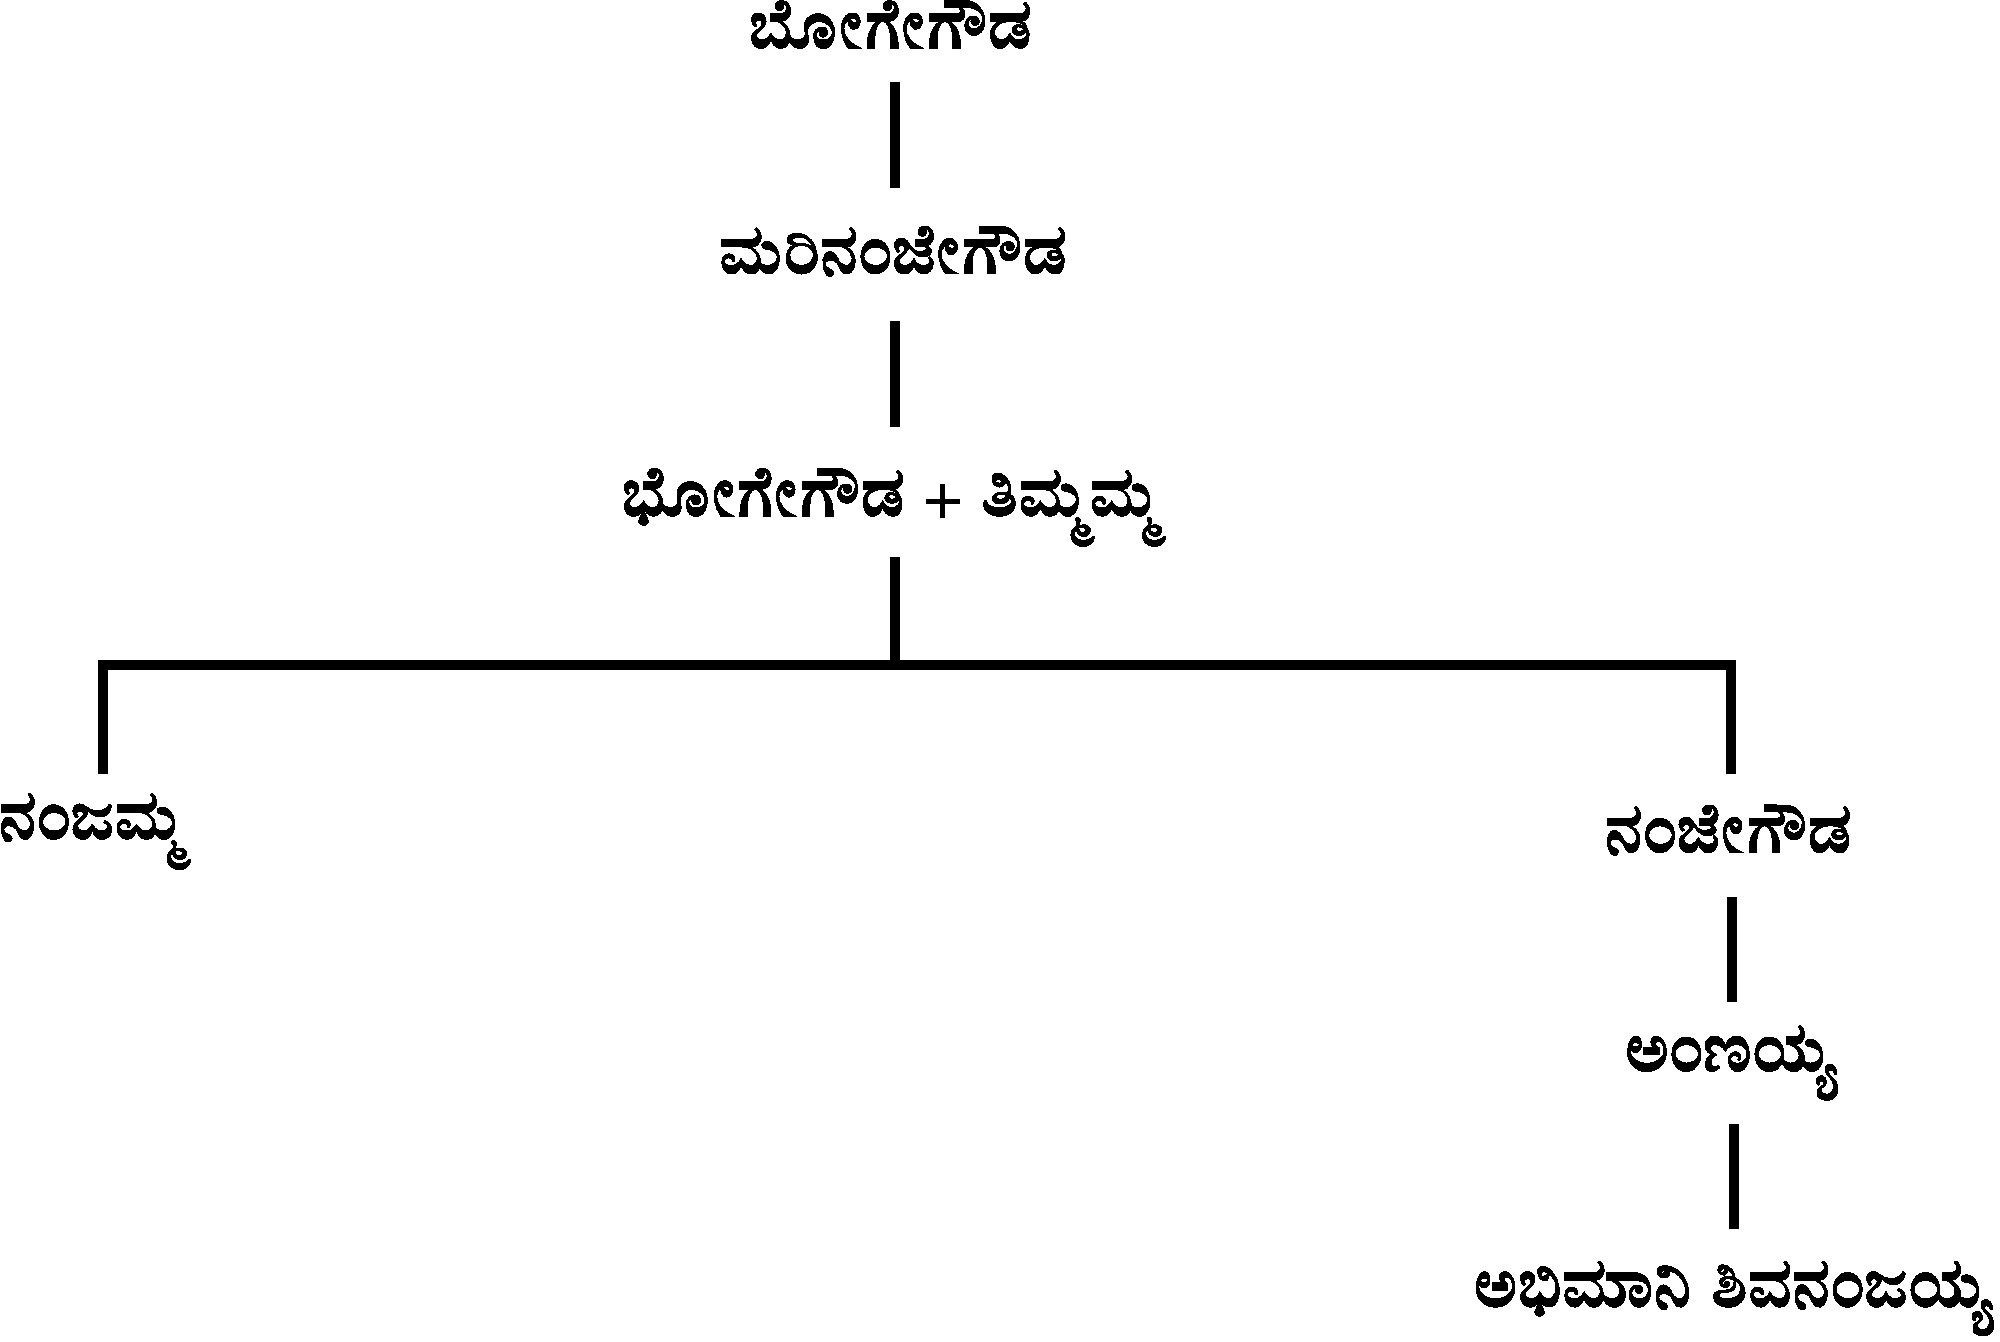
\includegraphics[scale=1.2]{images/chap3/chap3fig47.jpeg}
\end{figure}

ಮುಮ್ಮಡಿ ಕೃಷ್ಣರಾಜ ಒಡೆಯರ ಕಾಲದ ಶಾಸನಗಳಲ್ಲಿ ಮೇಲೆ ಹೇಳಿದ ಅನೇಕ ಅಧಿಕಾರಿ ಹುದ್ದೆಗಳು ಉಲ್ಲೇಖವಾಗಿವೆ. ‘ಶಿರಸ್ತೇದಾರ್​\index{ಶಿರಸ್ತೇದಾರ್​}’ ಸುಬ್ಬಯ್ಯನ ಮಗ ಅತಿಕುಪ್ಪೆ (ಇಂದಿನ ಕೃಷ್ಣರಾಜಪೇಟೆ) ತಾಲ್ಲೂಕು ‘ಮಾಮಲೆದಾರ್\index{ಮಾಮಲೆದಾರ್}​’ ಸುಬ್ಬರಾಯ.\endnote{ ಎಕ 6 ಪಾಂಪು 203 ಮೇಲುಕೋಟೆ 1867} ಮಂಡ್ಯ ‘ತಾಲ್ಲೂಕು ಅಮೀಲ\index{ತಾಲ್ಲೂಕು ಅಮೀಲ}’ (ಅಮಲ್ದಾರ್​) ತಿರುಕುಡಿ ಶ‍್ರೀನಿವಾಸರಾವು.\endnote{ ಎಕ 7 ಮಂ 1 ಮಂಡ್ಯ 1847} ಮುಮ್ಮಡಿ ಕೃಷ್ಣರಾಜ ಒಡೆಯರಿಂದ ಪೋಷಿತನಾದ ಕೂಡ್ಲುಕುಪ್ಪೆ ‘ಶಾನುಭಾಗ’ ಅಹೋಬಲಯ್ಯನ ತಮ್ಮ ‘ಅರಮನೆಯ ಶಿರಸ್ತೆದಾರ್\index{ಅರಮನೆಯ ಶಿರಸ್ತೆದಾರ್}​’ ಹಿರಣ್ಣಯ್ಯನ ಮಗ ಮೋದಿಖಾನೆ ಶಿರಸ್ತೇದಾರ್\index{ಮೋದಿಖಾನೆ ಶಿರಸ್ತೇದಾರ್}​’ ನರಸಯ್ಯ.\endnote{ ಎಕ 7 ಮ 12 ಮದ್ದೂರು 1865} ಮಳವಳ್ಳಿ ತಾಲ್ಲೂಕು ‘ಮಾಮಲೆದಾರ್​’ ಜೊಸೆಫ್​ ಸಿಬ್ಬಾಲ್​.\endnote{ ಎಕ 7 ಮವ 1 ಮಳವಳ್ಳಿ 1869} ಕರಣಿಕ ಗೋವಿಂದಯ್ಯ.\endnote{ ಎಕ 6 ಪಾಂಪು 204 ಮೇಲುಕೋಟೆ 18ನೇ ಶ.} ಖಾಸಾ ಬೊಕ್ಕಸದ ಲಿಂಗಾಚಾರಿಯ ಕುಮಾರ ಸುನಾರ್​ಖಾನೆಯ\index{ಸುನಾರ್​ಖಾನೆ}(ಒಡವೆ ವಸ್ತುಗಳ ಭಂಡಾರದ ಅಧಿಕಾರಿ ಇರಬಹುದು) ರಂಗಾಚಾರಿ.\endnote{ ಎಕ 6 ಶ‍್ರೀಪ 42 ಶ‍್ರೀರಂಗಪಟ್ಟಣ 1852} ಇವರುಗಳ ಉಲ್ಲೇಖವಿದೆ. ಕಂಮಗಾರ ಚಿಣ್ಣಯ್ಯ, ವೆಂಕಟಪತಯ್ಯ, ತಿಮ್ಮಪ್ಪಯ್ಯ ಇವರುಗಳು ನಾಗಮಂಗಲದ ಸೌಮ್ಯಕೇಶವದೇವಾಲಯವನ್ನು ಜೀರ್ಣೋದ್ಧಾರ ಮಾಡುತ್ತಾರೆ. ಕಮ್ಮಗಾರ ಎಂದರೆ ಅಕ್ಕಸಾಲಿಗರು ಅಥವಾ ವಿಶ್ವಕರ್ಮ ಜನಾಂಗದವರು. ನಾಗಮಂಗಲ ಇವರ ಪ್ರಸಿದ್ಧ ಕೇಂದ್ರವಾಗಿದೆ.\endnote{ ಎಕ 7 ನಾಮಂ 13 ನಾಗಮಂಗಲ 1845}


\section*{ಮಂಡ್ಯ ಜಿಲ್ಲೆಯ ಪ್ರಾಚೀನ ಆಡಳಿತ ವಿಭಾಗಗಳು\index{ಪ್ರಾಚೀನ ಆಡಳಿತ ವಿಭಾಗಗಳು}}

ಪ್ರಾಚೀನ ಕಾಲದಿಂದಲೂ ವಿಸ್ತಾರವಾದ ಸಾಮ್ರಾಜ್ಯವನ್ನು ಆಡಳಿತದ ಅನುಕೂಲಕ್ಕಾಗಿ ವಿಭಾಗ, ಉಪವಿಭಾಗಗಳನ್ನಾಗಿ ವಿಭಜಿಸಲಾಗುತ್ತಿತ್ತು. \textbf{ಇವುಗಳನ್ನು ಆಡಳಿತ ವಿಭಾಗಗಳು ಎಂದು }ಹೇಳಬಹುದು. “ಕರ್ನಾಟಕದ ಆಡಳಿತ ವಿಭಾಗಗಳ ಸೂಚನೆಗಾಗಿ ತೀರಾ ಪ್ರಾಚೀನ ಕಾಲದಲ್ಲಿ ಅಂದರೆ ಶಾತವಾಹನರ ಕಾಲದಲ್ಲಿ ಭುಕ್ತಿ, ರಟ್ಟ ಎಂಬ ಉತ್ತರ ಪದಗಳನ್ನು ಬಳಸಲಾಗಿದೆ. ಕದಂಬರ ಕಾಲದಲ್ಲಿ ವಿಷಯ, ಮಂಡಲ, ರಾಷ್ಟ್ರ, ಎಂಬವು ಉತ್ತರ ಪದಗಳು. ಬಾದಾಮಿ ಚಾಲುಕ್ಯರ ಕಾಲದಲ್ಲಿ ವಿಷಯ, ಆಹಾರ, ಭೋಗ, ರಾಷ್ಟ್ರ ಎಂಬ ಉತ್ತರ ಪದಗಳು ಕಾಣುತ್ತವೆ. ರಾಷ್ಟ್ರಕೂಟರ ಕಾಲದಿಂದ ನಾಡು, ನಾಟ್ಟು, ಮಂಡಲ, ವಿಷಯ, ಜನಪದ, ಭೋಗ ಪದಗಳು ಬಳಕೆಗೊಂಡಿವೆ. ಇದು ಕಲ್ಯಾಣಚಾಲುಕ್ಯ, ಕಲಚುರಿ, ಯಾದವ ಮತ್ತು ಹೊಯ್ಸಳರವರೆಗೆ ಮುಂದುವರಿದು, ವಿಜಯನಗರ ಕಾಲಕ್ಕೆ ಒಮ್ಮೆಲೇ, ರಾಜ್ಯ, ವೇಂಠೆ, ವೇಂಠಕ, ವಳಿತ, ಚಾವಡಿ, ಮಾಗಣಿ, ಸೀಮೆ ಪದಗಳು ಕಾಣಿಸಕೊಳ್ಳುತ್ತವೆ. ಮರಾಠರ ಕಾಲದಲ್ಲಿ ಮಹಲು ಇತ್ಯಾದಿ ಪದಗಳು ಬಳಕೆಯಾಗಿವೆ”, ಎಂದು ವಿದ್ವಾಂಸರು ಅಭಿಪ್ರಾಯ ಪಟ್ಟಿದ್ದಾರೆ.\endnote{ ಕಲಬುರ್ಗಿ, ಎಂ.ಎಂ., ಪ್ರಾಚೀನ ಕರ್ನಾಟಕದ ಆಡಳಿತ ವಿಭಾಗಗಳು, ಮುನ್ನುಡಿ, ಪುಟ vi - viii}

ಪ್ರಾಚೀನ ಕಾಲದಲ್ಲಿ ವಿಭಾಗಗಳು ಪ್ರಾಕೃತಿ ಪ್ರತಿಬಂಧಕಗಳಾದ, ನದಿ, ಬೆಟ್ಟಗಳಿಗೆ ಸೀಮಿತವಾಗಿ ನಿರ್ಧರಿತವಾಗು\-ತ್ತಿದ್ದವು. ಕೆಲವೊಮ್ಮೆ ಅನ್ಯ ರಾಜರ ಸೀಮಾರೇಖೆಗಳೂ ಇದನ್ನು ನಿರ್ಧರಿಸುತ್ತಿರಬಹುದು”.\endnote{ ಕಲಬುರ್ಗಿ, ಎಂ.ಎಂ., ಪ್ರಾಚೀನ ಕರ್ನಾಟಕದ ಆಡಳಿತ ವಿಭಾಗಗಳು, ಮುನ್ನುಡಿ, ಪುಟ vi - viii} “ತೀರಾ ಪ್ರಾಚೀನ ಕಾಲದಲ್ಲಿ ಇಂಥ ವಿಭಾಗಗಳನ್ನು ಆಹಾರ-ಮಂಡಲ-ಭುಕ್ತಿ-ವಿಷಯ-ದೇಶ ಎಂದು ಮುಂತಾಗಿ ಕರೆಯಲಾಗುತ್ತಿತ್ತು. ಮಧ್ಯಕಾಲೀನ ಕರ್ನಾಟಕ ಮತ್ತು ಡೆಕ್ಕನ್​ ಶಿಲಾಶಾಸನಗಳಲ್ಲಿ ಇವುಗಳಿಗೆ ಮಂಡಲ\index{ಮಂಡಲ}-ವಿಷಯ-ದೇಶ-ನಾಡು-ಕಂಪಣ\index{ಕಂಪಣ (ಕಂಪಣ್ಣ) ಒಡೆಯ, ಕಂಪ ಮಂತ್ರಿ, ಕಂಪರಾಜ} ಎಂಬ ಹೆಸರುಗಳನ್ನು ಬಳಸಲಾಗಿದೆ”, “ನಾಡು ಎಂಬ ಪದವನ್ನು ದೊಡ್ಡ, ಸಣ್ಣ, ಅತಿಸಣ್ಣ ವಿಭಾಗಗಳಿಗೂ ಬಳಸಿರುವುದರಿಂದ ಅದು ಸ್ಥೂಲವಾಗಿ ಪ್ರದೇಶ ಎಂಬ ಅರ್ಥವನ್ನು ನಿರ್ದೇಶಿಸಲು ಮಾತ್ರ ಬಳಕೆಯಾಗಿದೆ, ನಾಡು ಎಂದ ತಕ್ಷಣ ದೊಡ್ಡ ವಿಭಾಗವೆಂದು ತಿಳಿಯಬಾರದು” ಎಂದು ಡಾ. ಜೆ.ಎಂ.ನಾಗಯ್ಯನವರು ಹೇಳಿದ್ದಾರೆ.\endnote{ ನಾಗಯ್ಯ, ಡಾ॥ಜೆ.ಎಂ., ಆರನೆಯ ವಿಕ್ರಮಾದಿತ್ಯನ ಶಾಸನಗಳು-ಒಂದು ಅಧ್ಯಯನ, ಪುಟ 87-89}

ಗಂಗರ ಕಾಲದಲ್ಲಿ ರಾಜ್ಯವನ್ನು ನಾಡುಗಳಾಗಿ ವಿಭಜಿಸಲಾಗಿತ್ತು, ಈ ನಾಡುಗಳಿಗೆ ಗ್ರಾಮಸಂಖ್ಯಾಧಾರಿತ ಸಂಖ್ಯೆಗಳನ್ನು ನೀಡಲಾಗುತ್ತಿತ್ತು.\endnote{ ಸೂರ್ಯನಾಥಕಾಮತ್​, ಡಾ॥, ಕರ್ನಾಟಕದ ಸಂಕ್ಷಿಪ್ತ ಇತಿಹಾಸ, ಪುಟ 39} ಚಾಲುಕ್ಯರ ಕಾಲದಲ್ಲಿ ಸಾಮ್ರಾಜ್ಯವನ್ನು ಮಹಾರಾಷ್ಟ್ರಕಗಳಾಗಿ ವಿಭಜಿಸಿದ್ದು, ಅವುಗಳ ಕೆಳಗೆ ರಾಷ್ಟ್ರಕ ಅಥವಾ ಮಂಡಲಗಳಿದ್ದವು, ವಿಷಯ ಮುಂದಿನ ಕಿರುಭಾಗ. ಭೋಗ ಎಂಬ ಶಬ್ದವು ವಿಷಯಕ್ಕೆ ಸಮಾನವಾದುದೇ ತಿಳಿಯದು.\endnote{ ಅದೇ, ಪುಟ 49} ರಾಷ್ಟ್ರಕೂಟರ ಕಾಲದಲ್ಲಿ ರಾಜ್ಯವು ಮಂಡಲಗಳಾಗಿ ವಿಭಜಿತವಾಗಿದ್ದು, ಮಂಡಲವನ್ನು ರಾಷ್ಟ್ರವೆಂದು ಕರೆಯಲಾಗುತ್ತಿತ್ತು. ರಾಷ್ಟ್ರವನ್ನು ವಿಷಯ ಎಂಬ ಜಿಲ್ಲೆಗಳಾಗಿ ವಿಭಜಿಸಿದ್ದು, ವಿಷಯದ ನಂತರ ನಾಡು ಎಂಬ ಭಾಗವಿದ್ದು, ಆಡಳಿತದ ಕೊನೆಯ ಘಟಕ ಗ್ರಾಮವಾಗಿತು.\endnote{ ಅದೇ, ಪುಟ 64} ಕಲ್ಯಾಣದ ಚಾಲುಕ್ಯರ ಕಾಲದಲ್ಲಿ ಸಾಮ್ರಾಜ್ಯವನ್ನು ಪ್ರಾಂತಗಳಾಗಿ ವಿಭಜಿಸಲಾಗಿತ್ತು. ಪ್ರಾಂತಗಳನ್ನು ಮಂಡಲ, ದೇಶ, ರಾಷ್ಟ್ರ ಮುಂತಾಗಿ ಕರೆಯುತ್ತಿದ್ದರು. ಇವುಗಳ ಕೆಳಗೆ ನಾಡುಗಳೆಂಬ ಜಿಲ್ಲೆಗಳಿದ್ದವು. ಇದರ ಕೆಳಗೆ ಕಂಪಣಗಳೆಂಬ ಇಂದಿನ ಹೋಬಳಿಯಂತಹ ಗ್ರಾಮಗಳ ಗುಂಪಿತ್ತು ಆದರೆ ಈ ಆಡಳಿತ ವಿಭಾಗಗಳಲ್ಲಿ ಸಮಾನತೆ ಇರಲಿಲ್ಲ.\endnote{ ಅದೇ ಪುಟ 79}

ಹೊಯ್ಸಳರ ಕಾಲದ ಆಡಳಿತ ಘಟಕಗಳ ಹೆಸರುಗಳ ವ್ಯತ್ಯಾಸವನ್ನು ಗುರುತಿಸುವುದು ಕಷ್ಟ. ನಾಡು\index{ನಾಡು}, ವಿಷಯಗಳ\index{ವಿಷಯ} ಉಲ್ಲೇಖ ಶಾಸನಗಳಲ್ಲಿದ್ದು ಇವುಗಳಲ್ಲಿ ಯಾವುದು ಹಿರಿದು, ಯಾವುದು ಕಿರಿಯದು ತಿಳಿಯದು.\endnote{ ಅದೇ, ಪುಟ 97} ವಿಜಯನಗರ ಕಾಲದಲ್ಲಿ ಸಾಮ್ರಾಜ್ಯವನ್ನು ರಾಜ್ಯಗಳಾಗಿ ವಿಭಜಿಸಲಾಗಿತ್ತು. ರಾಜ್ಯವನ್ನು ವಿಷಯ, ವೇಂಟೆ ಎಂದು ವಿಭಜಿಸಲಾಗಿತ್ತು. ಈ ಭಾಗಕ್ಕೆ ಸೀಮೆ ಅಥವಾ ನಾಡು ಎಂಬ ಉಪವಿಭಾಗವಿದ್ದು, ಸ್ಥಳ ಅಥವಾ ಕಂಪಣ ಕೆಲವೇ ಗ್ರಾಮಗಳುಳ್ಳ ಕಡೆಯ ಭಾಗವಾಗಿತ್ತು.\endnote{ ಅದೇ, ಪುಟ 140} ಮೈಸೂರು ಅರಸರ ಕಾಲದಲ್ಲಿ ವಿಜಯನಗರ ಕಾಲದ ಆಡಳಿತ ವ್ಯವಸ್ಥೆ ಹೆಚ್ಚುಕಡಿಮೆ ಹಾಗೆಯೇ ಮುಂದುವರಿಯಿತು ಎಂಬುದು ವಿದ್ವಾಂಸರ ಅಭಿಪ್ರಾಯ.

“ಪ್ರಾಚೀನ ಕಾಲದಲ್ಲಿ ಆಡಳಿತದ ಅನುಕೂಲಕ್ಕಾಗಿ ಭೌಗೋಳಿಕವಾಗಿ ವಿಸ್ತಾರವಾಗಿದ್ದ ರಾಜ್ಯವನ್ನು ಮೂರು ಭಾಗಗಳಾಗಿ ವಿಂಗಡಿಸಿದ್ದರು. ಮಂಡಲ, ನಾಡು, ಊರು. ರಾಜಧಾನಿಯ ಸುತ್ತಣ ಭಾಗವನ್ನು ರಾಜನೇ ನೇರವಾಗಿ ಆಳುತ್ತಿದ್ದನು. ಉಳಿದ ರಾಜ್ಯವನ್ನು ಮಂಡಲಗಳನ್ನಾಗಿ ವಿಂಗಡಿಸಿ ಒಂದೊಂದು ಮಂಡಲಕ್ಕೂ ಮಂಡಲೇಶ್ವರರನ್ನು ನೇಮಿಸು\-ತ್ತಿದ್ದನು. ಒಂದೊಂದು ಮಂಡಲವನ್ನೂ ನಾಡುಗಳಾಗಿ ವಿಂಗಡಿಸಿ ಆಯಾ ನಾಡಿಗೆ ನಾೞ್ಪ್ರಭು ಅಥವಾ ನಾಡಗಾವುಂಡನನ್ನು ನೇಮಿಸು\-ತ್ತಿದ್ದರು. ನಾಡಿನ ಆಯಾ ಊರಿಗೆ ಮುಖ್ಯಸ್ಥನಾಗಿ ಪ್ರಭುಗಾವುಂಡ\index{ಪ್ರಭು ಗಾವುಂಡ (ಗಾವುಂಡರು) (ಗವುಡುಗಳು)} ಆಥವಾ ಊರಗಾವುಂಡನಿರುತ್ತಿದ್ದನು” ಎಂದು ವಿದ್ವಾಂಸರು ಹೇಳಿದ್ದಾರೆ.\endnote{ ಚಿದಾನಂದಮೂರ್ತಿ, ಎಂ., ಡಾ॥, ಕನ್ನಡ ಶಾಸನಗಳ ಸಾಂಸ್ಕೃತಿಕ ಅಧ್ಯಯನ, ಪುಟ 341}

ಈ ಅಂಶಗಳ ಹಿನ್ನೆಲೆಯಲ್ಲಿ ಮಂಡ್ಯ ಜಿಲ್ಲೆಯ ಪ್ರದೇಶದಲ್ಲಿ ಅಸ್ತಿತ್ವದಲ್ಲಿದ್ದ ಆಡಳಿತ ವಿಭಾಗಗಳನ್ನು ಪರಿಶೀಲಿಸ\-ಬಹುದು. ಸಂಖ್ಯಾ ಸೂಚಿತ ಆಡಳಿತ ವಿಭಾಗಗಳಿಗೆ ಕೆಲವೊಂದು ಸಲ ನಾಡು ಎಂಬ ವಿಶೇಷಣ ಇದ್ದರೆ ಕೆಲವು ಸಲ ಇರುವುದಿಲ್ಲ. ಸಂಖ್ಯಾ ಸೂಚಿ ಆಡಳಿತ ವಿಭಾಗಗಳನ್ನು, ಅವುಗಳ ಮುಖ್ಯ ಸ್ಥಳದ ಹೆಸರಿನಲ್ಲಿ ಕರೆಯಲಾಗಿದೆ. ಆಡಳಿತ ವಿಭಾಗಗಳ ಮುಂದೆ ಇರುವ ಸಂಖ್ಯೆಗಳು, ಆ ನಾಡಿನಲ್ಲಿ ಇದ್ದ ಹಳ್ಳಿಗಳು ಮತ್ತು ಕಾಲುವಳ್ಳಿಗಳ ಸಂಖ್ಯೆಯನ್ನು ಸೂಚಿಸುತ್ತದೆ ಎಂದು ಹೇಳಿರುವ ಅಭಿಪ್ರಾಯ ಸೂಕ್ತವಾಗಿದೆ.\endnote{ ಅದೇ, ಪುಟ 87} ಮಹಾನಾಡು\index{ಮಹಾನಾಡು} ದೊಡ್ಡ ಪ್ರದೇಶದ ಸಂಘ(ಡಿಸ್ಟ್ರಿಕ್ಟ್​ ಅಸೆಂಬ್ಲಿ)ಎಂದೂ, ನಾಡು ಕೆಲವು ಹಳ್ಳಿಗಳ ಗುಂಪಿನ ಸಂಘವೆಂದೂ ದೀಕ್ಷಿತ್​ ಅವರು ಹೇಳಿದ್ದಾರೆ.\endnote{ \engfoot{Dixith, Dr.G.S., Local Self Government in Mediaveal Karnataka, pp 35}}

\section*{ಗಂಗವಾಡಿ ತೊಂಬತ್ತರುಸಾಸಿರ}

ಗಂಗರು ಮತ್ತು ಹೊಯ್ಸಳರ ಕಾಲದಲ್ಲಿ ಮಂಡ್ಯ ಜಿಲ್ಲೆಯು ಗಂಗವಾಡಿ 96000ದ ಒಂದು ಭಾಗವಾಗಿತ್ತು. ಅನೇಕ ಶಾಸನಗಳಲ್ಲಿ ಗಂಗವಾಡಿಯನ್ನು, ಗಂಗಮಂಡಲವೆಂದು ಕರೆದಿದೆ. ಜಿಲ್ಲೆಯಲ್ಲಿ ದೊರಕಿರುವ ಕ್ರಿ.ಶ.776ರ ಗಂಗರ ಪ್ರಾಚೀನ ಸಂಸ್ಕೃತ ತಾಮ್ರ ಶಾಸನದಲ್ಲಿ ಇದನ್ನು “ಷಣ್ಣವತಿಸಹಸ್ರ ವಿಷಯ\index{ಷಣ್ಣವತಿಸಹಸ್ರ ವಿಷಯ}” ಎಂದು ಕರೆದಿದೆ.\endnote{ ಎಕ 7 ನಾಮಂ 149 ದೇವರಹಳ್ಳಿ 776} ಇಮ್ಮಡಿ ಮಾರಸಿಂಹನ ಕ್ರಿ.ಶ.972ರ ಆರಣಿ ಶಾಸನ\-ದಲ್ಲಿ.\endnote{ ಎಕ 7 ನಾಮಂ 99 ಆರಣಿ 972} “ಗಂಗವಾಡಿ ತೊಂಬತ್ತರುಸಾಸಿರ\index{ಗಂಗವಾಡಿ ತೊಂಭತ್ತರುಸಾಸಿರ}” ಎಂದು ಹೇಳಿರುವುದೇ ಜಿಲ್ಲೆಯಲ್ಲಿ ದೊರಕಿರುವ ಈ ಹೆಸರಿನ ಅತ್ಯಂತ ಪ್ರಾಚೀನ ಉಲ್ಲೇಖ. ಕ್ರಿ.ಶ.986ರ ಕಾಡುಕೊತ್ತನಹಳ್ಳಿ\index{ಕಾಡುಕೊತ್ತನಹಳ್ಳಿ} ಶಾಸನದಲ್ಲ.\endnote{ ಎಕ 7 ಮ 116 ಕಾಡುಕೊತ್ತನಹಳ್ಳಿ 986} “ಬಲ್ಲಪಂ ಗಂಗವಾಡಿಗೆ ಬಂದ” ಎಂದು ಹೇಳಿದೆ. ಬಲಮುರಿಯ ರಾಜರಾಜ ಚೋಳನ ಶಾಸನದಲ್ಲ.\endnote{ ಎಕ 6 ಶ‍್ರೀಪ 78 ಬಲಮುರಿ 1012} “ಶ‍್ರೀ ಗಂಗಾವನಿರಟ್ಟ\index{ಶ‍್ರೀ ಗಂಗಾವನಿರಟ್ಟ}” ಎಂದು ಕರೆಯಲಾಗಿದೆ. ಹೊಯ್ಸಳರ ವಿನಯಾದಿತ್ಯನ ಕಿಕ್ಕೇರಿ ಶಾಸನದಲ್ಲ.\endnote{ ಎಕ 6 ಕೃಪೇ 37 ಕಿಕ್ಕೇರಿ 1095} “ಗಂಗಮಂಡಳ” ಎಂದು ಹೇಳಿದೆ. ಕ್ರಿ.ಶ.1165ರ ಲಾಳನಕೆರೆ\index{ಲಾಳನಕೆರೆ} ಶಾಸನದಲ್ಲ.\endnote{ ಎಕ 7 ನಾಮಂ 63 ಲಾಳನಕೆರೆ 1165} “ಗಂಗರಾಜ್ಯ” ಎಂದು ಕರೆದಿದೆ. ಇದೇ ಕಾಲದ ಕ್ರಿ.ಶ.1224ರ ಬೆಳ್ಳೂರು ಶಾಸನದಲ್ಲಿದಲ್ಲಿ ನಾರಸಿಂಹನನ್ನು “ಗಂಗದೇಶಾಧಿಪ\index{ಗಂಗದೇಶಾಧಿಪ}” ಎಂದು ಕರೆದಿದೆ. ಉಳಿದಂತೆ ಜಿಲ್ಲೆಯಲ್ಲಿ ದೊರಕಿರುವ ಬಹುತೇಕ ಹೊಯ್ಸಳರ ಕಾಲದ ಶಾಸನಗಳಲ್ಲಿ ಗಂಗವಾಡಿ ತೊಂಬತ್ತರುಸಾಸಿರ ಅಥವಾ ಗಂಗವಾಡಿ ಎಂದು ಕರೆಯಲಾಗಿದೆ. “ಕ್ರಿ.ಶ.ಸುಮಾರು 4ನೇ ಶತಮಾನದ ವೇಳೆಗೆ ಈ ಪ್ರದೇಶವು ಪಲ್ಲವರ ಮಾಂಡಲೀಕರಾಗಿದ್ದ, ಮೂಲತಃ ಕೊಂಗುನಾಡಿನ ಅಧಿಪತಿಗಳಾಗಿದ್ದ ಗಂಗರ ಆಳ್ವಿಕೆಗೆ ಒಳಪಟ್ಟಿತ್ತೆಂದು ವಿದ್ವಾಂಸರು ಹೇಳಿದ್ದಾರೆ”.\endnote{ ಕೃಷ್ಣಮೂರ್ತಿ ಡಾ॥ ಪಿ.ವಿ., ಮಂಡ್ಯ ಜಿಲ್ಲಾ ಪ್ರದೇಶದ ಚಾರಿತ್ರಿಕ ಆಡಳಿತ ಘಟಕಗಳು,

ಮಂಡ್ಯ ಜಿಲ್ಲೆಯ ಇತಿಹಾಸ ಮತ್ತು ಪುರಾತತ್ವ, ಪುಟ 278} ಮುಂದೆ ಗಂಗರು ಕೊಂಗುನಾಡನ್ನು ತೊರೆದು ನಂದಗಿರಿ, ಮಣ್ಣೆ, ಕೊಳಾಲದ ಮೂಲಕ ತಲಕಾಡಿಗೆ ಬಂದು ನೆಲೆಸಿದರು. ಗಂಗರು ಈ ಪ್ರದೇಶವನ್ನು ಸತತವಾಗಿ ಬಹಳ ವರ್ಷಗಳ ಆಳುತ್ತಿದ್ದುದರಿಂದ ಅವರಿಂದಲೇ ಈ ಹೆಸರು ಬಂದಿರಬಹುದು.

ಒಂದನೆಯ ಬಲ್ಲಾಳನ ಕ್ರಿ.ಶ.1103ರ ಶಾಸನದಲ್ಲಿ “ಗಂಗವಾಡಿ ತೊಂಬತ್ತರುಸಾಸಿರಮಂ ಸುಖಸಂಕಥಾ\break ವಿನೋದಿಂದಾಳೆ” ಎಂಬುದೇ ಜಿಲ್ಲೆಯಲ್ಲಿ ದೊರಕಿರುವ, ಹೊಯ್ಸಳರ ಕಾಲದ ಮೊದಲ ಪ್ರಯೋಗ. ನಂತರ ಕ್ರಿ.ಶ.1118ರ ಹೊಸಹೊಳಲು ಶಾಸನದಲ್ಲಿ “ಭುಜಬಳವೀರಗಂಗ ಪೊಯ್ಸಳದೇವರು ಗಂಗವಾಡಿ ತೊಂಬತ್ತರುಸಾಸಿರಮನೇಕ ಛತ್ರ\break ಛಾಯೆಯಿಂ ಪೃಥ್ವೀರಾಜ್ಯಂಗೆಯುತ್ತಿರೆ” ಎಂದು ಹೇಳಿದೆ. ಕ್ರಿ.ಶ.1132ರ ವೈದ್ಯನಾಥಪುರ\index{ವೈದ್ಯನಾಥಪುರ} ಶಾಸನದಲ್ಲಿ ಗಂಗವಾಡಿ ತೊಂಬತ್ತರುಸಾವಿರ, ನೊಳಂಬವಾಡಿ ಮೂವತ್ತರ್ಛಾಸಿರ\index{ನೊಳಂಬವಾಡಿ ಮೂವತ್ತರ್ಛಾಸಿರ}, ಬನವಸೆ ಪನ್ನಿರ್ಛಾಸಿರ\index{ಬನವಸೆ ಪನ್ನಿರ್ಛಾಸಿರ}, ಹಾನುಂಗಲಯ್ನೂರುಗಳನ್ನು\index{ಹಾನುಂಗಲಯ್ನೂರು}\break ವಿಷ್ಣುವರ್ಧನನು ಆಳುತ್ತಿದ್ದನೆಂದು ಹೇಳಿದೆ. ಅಂದರೆ ಗಂಗವಾಡಿಯಲ್ಲಿ, ಉಳಿದವು ಸೇರಿಲ್ಲವೆಂದಾಯಿತು.

\section*{ಹೊಯ್ಸಳ ದೇಶ/ರಾಜ್ಯ/ನಾಡು/ಮಂಡಲ}

ಹೊಯ್ಸಳ ಸಾಮ್ರಾಜ್ಯವು, ಗಂಗವಾಡಿಯ ಭಾಗವೇ ಆಗಿತ್ತು. ಆದರೂ ಹೊಯ್ಸಳರ ಕಾಲದಿಂದಲೂ ಅಲ್ಲಲ್ಲಿ ಈ ಪ್ರದೇಶವನ್ನು ಹೊಯ್ಸಳರಾಜ್ಯ, ಹೊಯ್ಸಳ ಮಂಡಲ ಎಂದು ಕರೆದಿರುವುದನ್ನು ಈಗಾಗಲೇ ಗಮನಿಸಲಾಗಿದೆ. ಆದರೆ ಹೊಯ್ಸಳರು ಗಂಗರಮೇಲಿನ ಅಭಿಮಾನದಿಂದ ಗಂಗವಾಡಿ ಎಂಬ ಹೆಸರನ್ನೇ ಉಳಿಸಿಕೊಂಡು ಬಂದರೂ ಅವರ ಶಾಸನಗಳಲ್ಲಿಯೂ ಹೊಯ್ಸಳರಾಜ್ಯ ಎಂದು ಬಳಕೆಯಾಗಿರುವುದು ಕಂಡುಬರುತ್ತದೆ. ತ್ರಿಭುವನಮಲ್ಲ ಪೊಯ್ಸಳದೇವರಾಜ್ಯದಲ್ಲಿ\index{ತ್ರಿಭುವನಮಲ್ಲ ಪೊಯ್ಸಳದೇವರಾಜ್ಯ} ಕಳ್ಬಪ್ಪು ಸಾಯಿರವೂ\index{ಕಳ್ಬಪ್ಪು ಸಾಯಿರ} ಸೇರಿದಂತೆ, ತಳಕಾಡು ಪಟ್ಟಣ\index{ತಲಕಾಡು ಪಟ್ಟಣ}, ಎಡದರೆಸಾಯಿರ\index{ಎಡದೊರೆ ಸಾಯಿರ}, ಕಿರುನಗರ\index{ಕಿರುನಗರ (ಕಿರುವೆಳ್ನಗರ)} ಸೇರಿದಂತೆ ಹದಿನೆಂಟು ವಿಷಯಗಳಿದ್ದವೆಂದು ಹೇಳಿದೆ.\endnote{ ಎಕ 6 ಕೃಪೇ 50 ತೊಣಚಿ 1048} ಇದರಲ್ಲಿ ಕಳ್ಬಪ್ಪು ಸಾಯಿರ ಮತ್ತು ಎಡದರೆ ಸಾಸಿರ ಮಾತ್ರ ಎರಡು ವಿಷಯಗಳು. ಉಳಿದವು ಎರಡು ಪಟ್ಟಣಗಳು. ಲಾಳನಕೆರೆಯ ಶಾಸನದಲ್ಲಿ ಏಚಿದಂಡಾಧಿಪನನ್ನು “ಹೊಯ್ಸಳರಾಜ್ಯ ಸಮುದ್ಧರಣ” ಎಂದು ಕರೆಯಲಾಗಿದೆ.\endnote{ ಎಕ 7 ನಾಮಂ 61 ಲಾಳನಕೆರೆ 1138} ಇದೇ ಲಾಳನಕೆರೆಯ ಪೂರ್ವೋಕ್ತ ಶಾಸನದಲ್ಲಿ “ಹೊಯ್ಸಳ ರಾಜ್ಯಲಕ್ಷ್ಮಿ\index{ಹೊಯ್ಸಳ ರಾಜ್ಯಲಕ್ಷ್ಮಿ}” ಎಂಬ ಉಲ್ಲೇಖವಿದೆ. ಕ್ರಿ.ಶ.1190ರ ಕಸಲಗೆರೆ ಶಾಸನದಲ್ಲಿ ಮಹದೇವದಂಡನಾಯಕನನ್ನು “ಹೊಯ್ಸಳರಾಜ್ಯ\index{ಹೊಯ್ಸಳರಾಜ್ಯ} ಪಯೋಜಭಾನು” ಎಂದು ಕರೆದಿದೆ.\endnote{ ಎಕ 7 ನಾಮಂ 168 ಕಸಲಗೆರೆ 1190} ಮೂರನೆಯ\break ಬಲ್ಲಾಳನ ಕಾಲಕ್ಕಾಗಲೇ ಗಂಗವಾಡಿ ಎಂಬ ಪ್ರಯೋಗ ಕಡಿಮೆಯಾಗುತ್ತಾ ಬಂದು ಹೊಯ್ಸಣ ನಾಡು\index{ಹೊಯ್ಸಣ ನಾಡು}.\endnote{ ಎಕ 6 ಕೃಪೇ 8 ಹೊಸಹೊಳಲು 1306} ಹೊಯ್ಸಳ ಮಂಡಲ.\endnote{ ಎಕ 6 ಕೃಪೇ 11 ಹರಿಹರಪುರ 1322, ಕೃಪೇ 108 ವರಹಾನಾಥಕಲ್ಲಹಳ್ಳಿ 1332} ಎಂದು ಕರೆಯಲಾಗಿದೆ.

ಜಿಲ್ಲೆಯಲ್ಲಿರುವ, ವಿಜಯನಗರದ ಕಾಲದ ಯಾವುದೇ ಶಾಸನಗಳಲ್ಲೂ ಗಂಗವಾಡಿ ಎಂಬ ಪ್ರಯೋಗ ಕಂಡು ಬರುವುದಿಲ್ಲ. ಹೊಯ್ಸಳರಿಂದ ತಮಗೆ ಬಂದ ಈ ಪ್ರದೇಶವನ್ನು, ವಿಜಯನಗರದ ಅರಸರು, ಹೊಯ್ಸಳರ ರಾಜ್ಯ/ದೇಶ/ಸೀಮೆ ಎಂದೇ ಕರೆಯತೊಡಗಿದರು. ಉದಾಹರಣೆಗೆ 1447 ಶ‍್ರೀರಂಗಪಟ್ಟಣ ಶಾಸನದಲ್ಲಿ “ಹೊಯ್ಸಣಾಖ್ಯಸ್ಯ ದೇಶಸ್ಯ\index{ಹೊಯ್ಸಣಾಖ್ಯಸ್ಯ ದೇಶಸ್ಯ} ಕಂನಂಬಾಡಿ ಸ್ಥಳೇ ಮೋದುನಾಡುಕೇ\index{ಮೋದುನಾಡು}”.\endnote{ ಎಕ 6 ಶ‍್ರೀಪ 21 ಶ‍್ರೀರಂಗಪಟ್ಟಣ 1447} 1458ರ ಮೇಲುಕೋಟೆ ಶಾಸನದಲ್ಲಿ “ಹೊಯಿಸಳರಾಜ್ಯದ\index{ಹೊಯಿಸಳರಾಜ್ಯ} ಕುರುವಂಕನಾಡ ವೇಂಠೆಯ\index{ಕುರುವಂಕನಾಡ ವೇಂಟೆಯ (ವೇಂಕೆಯ)}”.\endnote{ ಎಕ 6 ಪಾಂಪು 179 ಮೇಲುಕೋಟೆ 1458} 1462ರ ಕೈಗೋನಹಳ್ಳಿ ಶಾಸನದಲ್ಲಿ “ದೇಶೇ ಹೊಯಿಸಣ ಸಂಜ್ಞಿಕೇ”.\endnote{ ಎಕ 6 ಕೃಪೇ 71 ಕೈಗೋನಹಳ್ಳಿ 1462} 1532ರ ಬ್ಯಾಲದಕೆರೆ ಶಾಸನದಲ್ಲಿ “ಹೊಯಿಸಣಾಭಿಧೇ\break ದೇಶೇ ತು ಸಿಂಧಘಟ್ಟಸ್ಯ ಸೀಮಾಂತವರ್ತಿನ”.\endnote{ ಎಕ 6 ಕೃಪೇ 99 ಬ್ಯಾಲದಕೆರೆ 1532} 1533ರ ಅಚ್ಯುತರಾಯನ ಹುರಗಲವಾಡಿ ಶಾಸನದಲ್ಲಿ\break ಮಹಾಹೋಸಲನಾಡು ಎಂದು ಜಿಲ್ಲೆಯ ಶಾಸನಗಳಲ್ಲಿ ಉಲ್ಲೇಖಿಸಲಾಗಿದೆ.\endnote{ ಎಕ 7 ಮ 144 ಹುರುಗಲವಾಡಿ 1533}

ಮೈಸೂರು ಅರಸರ ಕಾಲದಲ್ಲೂ ಕೂಡಾ ಇದನ್ನು ಹೊಯ್ಸಳನಾಡು, ಹೊಯ್ಸಳದೇಶ\index{ಹೊಯ್ಸಳದೇಶ} ಎಂದೇ ಕರೆಯಲಾಗಿದೆ. 1663ರ ದೇವರಾಜ ಒಡೆಯರ ಮಾಳಗೂರು ಶಾಸನದಲ್ಲಿ “ವಿಕ್ರಮಾರ್ಜಿತವಾಗಿ ಬಂದ ಹೊಯ್ಸಲನಾಡ\index{ಹೊಯ್ಸಲನಾಡ}” ಎಂದು ಹೇಳಿದೆ.\endnote{ ಎಕ 6 ಕೃಪೇ 65 ಮಾಳಗೂರು 1663} 1673ರ ಹುಳ್ಳಂಬಳ್ಳಿ ಶಾಸನದಲ್ಲಿ “ಶ‍್ರೀಹೋಸಲನಾಡಿನ ಮೈಸೂರು ನಗರ”, 1722ರ ತೊಣ್ಣೂರು ಶಾಸನದಲ್ಲಿ “ರಮ್ಯೇ ಹೊಯ್ಸಳ ದೇಶಾಖ್ಯೇ\index{ಹೊಯ್ಸಳ ದೇಶಾಖ್ಯೇ}” ಎಂದು ಹೇಳಿದೆ. ಹೀಗೆ ಗಂಗವಾಡಿಯ ಹೊಯ್ಸಳ ನಾಡಾಗಿ ಬದಲಾಯಿತು.

\section*{ಕರ್ಣಾಟ\index{ಕರ್ಣಾಟ}/ಕರ್ಣಾಟಕ\index{ಕರ್ಣಾಟಕ}/ಕರ್ನಾಟ\index{ಕರ್ನಾಟ}/ಕರ್ನಾಟಕ\index{ಕರ್ನಾಟಕ}}

ಕನ್ನಡನಾಡಿನ ಉತ್ತರ ಭಾಗವನ್ನು ಕುಂತಲವೆಂದೂ, ತುಂಗಭದ್ರೆಯ ಕೆಳಗಣ ದಕ್ಷಿಣ ಭಾಗವನ್ನು ಕರ್ನಾಟ/ಕರ್ಣ್ನಾಟ/ಕ\break ಎಂದೂ ಕಲ್ಯಾಣದ ಚಾಲುಕ್ಯರ ಕಾಲದ ಶಾಸನಗಳಲ್ಲಿ ಹೇಳಿದೆ. ಕರ್ಣಾಟ ಮತ್ತು ಕುಂತಲಗಳು ಕನ್ನಡನಾಡಿನ ಕೇಂದ್ರಗಳಾ\-ಗಿದ್ದವು.\endnote{ ವೆಂಕಟಾಚಲ ಶಾಸ್ತ್ರೀ, ಡಾ॥ ಟಿ.ವಿ., ನಮ್ಮ ಕರ್ನಾಟಕ, ಪುಟ 76} ಕರ್ಣಾಟಕ, ಕುಂತಲ ಎರಡೂ ಸೇರಿ ಕನ್ನಡನಾಡು ಅಥವಾ ದೇಶವಾಗಿತ್ತೆಂದು ಹೇಳಬಹುದು. ಬಿಲ್ಹಣನು ತನ್ನ\break ವಿಕ್ರಮಾಂಕದೇವ ಚರಿತದಲ್ಲಿ ಆರನೆಯ ವಿಕ್ರಮಾದಿತ್ಯನು ಕುಂತಲೇಂದ್ರ ಮತ್ತು ಕರ್ನಾಟಕೇಂದುವಾಗಿದ್ದನೆಂದು ಹೇಳಿದ್ದಾನೆ.

ಮಂಡ್ಯ ಜಿಲ್ಲೆಯ ಪ್ರದೇಶವು ಕರ್ಣಾಟಕದ ಅಖಂಡ ಭಾಗವಾಗಿತ್ತು. ಈ ಪ್ರದೇಶವನ್ನು ಗಂಗವಾಡಿ, ಹೊಯ್ಸಳರಾಜ್ಯ ಎಂದು ಕರೆಯುವುದರ ಜೊತೆಗೆ, ಕರ್ನಾಟ, ಕರ್ಣಾಟ, ಕರ್ಣಾಟಕ, ಕರ್ನಾಟಕ ಎಂದೂ ಕರೆಯಲಾಗುತ್ತಿತ್ತು ಎನ್ನುವ ಬಹಳ ಮುಖ್ಯವಾದ ಅಂಶ ಶಾಸನಗಳಿಂದ ತಿಳಿದುಬರುತ್ತದೆ. ವಿಜಯನಗರ ಅರಸರು ಮತ್ತು ಮೈಸೂರು ಒಡೆಯರ ಕಾಲದಲ್ಲಿ ಕರ್ನಾಟಕ ಪದದ ಪ್ರಯೋಗವಿದೆ. ಇಮ್ಮಡಿದೇವರಾಯನನ್ನು ಕ್ರಿ.ಶ.1447ರ ಶ‍್ರೀರಂಗಪಟ್ಟಣ ತಾಮ್ರಶಾಸನದಲ್ಲಿ.\endnote{ ಎಕ 6 ಶ‍್ರೀಪ 21 ಶ‍್ರೀರಂಗಪಟ್ಟಣ 1447} “ಕರ್ನಾಟ ದೇಶಶ‍್ರೀ\index{ಕರ್ನಾಟ ದೇಶಶ‍್ರೀ} ಸ್ಥಿರತಾಟಂಕವತ್ಯಭೂತ್​” ಎಂದು ಕರೆಯಲಾಗಿದೆ. ಸುಜ್ಜಲೂರು ಶಾಸನದಲ್ಲ,\endnote{ ಎಕ 7 ಮವ 139 ಸುಜ್ಜಲೂರು 1473} ವೀರವಿರೂಪಾಕ್ಷನನ್ನು “ಕರ್ನಾಟಲಕ್ಷ್ಮೀ\index{ಕರ್ನಾಟಲಕ್ಷ್ಮೀ} ಸವಿಲಾಸಮಾಸ ಯಸ್ಮಿನ್​ ಮಹೀಪೇ ಮಹನೀಯ ಕೀರ್ತೌ” ಎಂದೂ, “ಕರ್ನಾಟೇಶ್ವರರಾಯ\index{ಕರ್ನಾಟೇಶ್ವರರಾಯ} ಕುಂಜರ ವಿರೂಪಾಕ್ಷ ಕ್ಷಮಾಧೀಶತಾ” ಎಂದೂ ಕರೆದಿದೆ. “ಕರ್ನ್ನಾಟ ದೇಶಶ‍್ರೀ” ಎಂದು ನೆಲಮನೆ ಶಾಸನದಲ್ಲಿ.\endnote{ ಎಕ 6 ಶ‍್ರೀಪ 93 ನೆಲಮನೆ 1485} “ರಂಗ ಕ್ಷಿತೀಂದ್ರ ಪಾಲಿತ ಮಹಾಕರ್ಣಾಟ ರಾಜ್ಯಶ‍್ರೀ\index{ಮಹಾಕರ್ಣಾಟ ರಾಜ್ಯಶ‍್ರೀ}” ಎಂದು ಸದಾಶಿವರಾಯನ ಹೊನ್ನೇನಹಳ್ಳಿ ಶಾಸನದಲ್ಲಿ.\endnote{ ಎಕ 7 ನಾಮಂ 107 ಹೊನ್ನೇನಹಳ್ಳಿ 1545} “ಕರ್ನಾಟ ದೇಶ\index{ಕರ್ನಾಟ ದೇಶ}” ಎಂದು ಶ‍್ರೀರಂಗಪಟ್ಟಣ ಶಾಸನದಲ್ಲಿ.\endnote{ ಎಕ 6 ಶ‍್ರೀಪ 21 ಶ‍್ರೀಪ 1686} “ಸ್ವಕೀಯಕರ್ನಾಟಕಕ\index{ಸ್ವಕೀಯಕರ್ನಾಟಕ} ರಾಜ್ಯಮಧ್ಯೇ” ಮತ್ತು “ಯಾದವ ಕುಲೋದ್ಧರಣ ಧುರೀಣ ಕರ್ನ್ನಾಟಕ ಚಕ್ರವರ್ತಿ\index{ಕರ್ನ್ನಾಟಕ ಚಕ್ರವರ್ತಿ} ಕೃಷ್ಣರಾಜ” ಎಂದು ತೊಣ್ಣೂರು ಶಾಸನದಲ್ಲಿ.\endnote{ ಎಕ 6 ಪಾಂಪು 99 ತೊಣ್ಣೂರು 1722} “ಕರ್ನಾಟ ದೇಶ\index{ಕರ್ನಾಟ ದೇಶ} ರಮಣೀಯ” ಎಂದು ಮೇಲುಕೋಟೆ ಶಾಸನದಲ್ಲಿ.\endnote{ ಎಕ 6 ಪಾಂಪು 215 ಮೇಲುಕೋಟೆ 1724} “ನಿರ್ಜಿತ್ಯ ಕರ್ನಾಟಕೇ\index{ಕರ್ನಾಟಕ} ಪದಾದ್ವಿಪ್ರಗಣೇ” ಎಂದು ಮಳವಳ್ಳಿ ಶಾಸನದಲ್ಲಿ.\endnote{ ಎಕ 7 ಮವ 2 ಮಳವಳ್ಳಿ 1685} ಹೇಳಿದೆ. ಮಂಡ್ಯ ಜಿಲ್ಲೆಯ ಈ ಭೂಭಾಗವು ಅಂದೇ ಕರ್ನಾಟಕ ರಾಜ್ಯದ ಭಾಗವಾಗಿತ್ತು.

\section*{ಮೈಸೂರು ಸೀಮೆ\index{ಮೈಸೂರು ಸೀಮೆ}/ಮೈಸೂರು ಸಂಸ್ಥಾನ\index{ಮೈಸೂರು ಸಂಸ್ಥಾನ}}

ಏಕೀಕರಣ ಪೂರ್ವದಲ್ಲಿ ಮತ್ತು ನಂತರದಲ್ಲಿ ಕರ್ನಾಟಕ ಎಂದು ಹೆಸರಿಡುವುದಕ್ಕೆ ಮುನ್ನ ನಮ್ಮ ಹಳೆಯ ಮೈಸೂರು ರಾಜ್ಯವನ್ನು ಮೈಸೂರು ಸೀಮೆ, ಮೈಸೂರು ಸಂಸ್ಥಾನ ಎಂದು ಕರೆಯಲಾಗುತ್ತಿತ್ತು. ಶಾಸನಗಳಲ್ಲಿ ಮಂಡ್ಯ ಜಿಲ್ಲೆಯ ಪ್ರದೇಶವು ಮೈಸೂರು ಸೀಮೆಗೆ ಅಥವಾ ಸಂಸ್ಥಾನಕ್ಕೆ ಸಲ್ಲುತ್ತಿತ್ತೆಂದು ಹೇಳಿದೆ. ಶ‍್ರೀರಂಗಪಟ್ಟಣ ತಾಲ್ಲೂಕು ಬೆಳಗೊಳ ಶಾಸನದಲ್ಲಿ “ಮೈಸೂರು ಚಾಮರಸವೊಡೆಯರ\index{ಮೈಸೂರು ಚಾಮರಸ ಒಡೆಯರು} ಮಕ್ಕಳು ಬೆಟ್ಟದ ಚಾಮರಸವೊಡೆಯರು” ಎಂದು ಹೇಳಿದ್ದು, ಈ ವೇಳೆಗೆ ಅವರು ಮೈಸೂರಿನಿಂದ ಆಳ್ವಿಕೆ ನಡೆಸುತ್ತಿದ್ದರೆಂದು ಹೇಳಬಹುದು.\endnote{ ಎಕ 6 ಶ‍್ರೀಪ 71 ಬೆಳಗೊಳ 1598} “ಮೈಸೂರು ನರಸರಾಜೊಡೆಯ\index{ಮೈಸೂರು ನರಸರಾಜೊಡೆಯ} ಕುಮಾರ ಚಾಮರಾಜೊಡೆಯರು.\endnote{ ಎಕ 6 ಪಾಂಪು 250 ಆನೆಗೊಳ 1620} “ಮಯಿಸೂರು ಚಾಮರಾಜೊಡೆಯರ\index{ಮಯಿಸೂರು ಚಾಮರಾಜೊಡೆಯರು} ಮಕ್ಕಳು ದೇವರಾಜರು”.\endnote{ ಎಕ 6 ಶ‍್ರೀಪ 111 ಅರಕೆರೆ 1625} “ಮೈಸೂರು ದೇವರಾಜ ಭೂಪಾಲ\index{ಮೈಸೂರು ದೇವರಾಜ ಭೂಪಾಲ} ಚಾಮರಾಜೇಂದ್ರ ಒಡೆಯರು, ಮೈಸೂರು ರಾಜೊಡೆಯರ\index{ಮೈಸೂರು ರಾಜೊಡೆಯರು} ಪೌತ್ರ ನರಸರಾಜೊಡೆಯರ ಪುತ್ರ ಚಾಮರಾಜೊಡೆಯರು”.\endnote{ ಎಕ 7 ವಮ 64 ಹೊನ್ನಲಗೆರೆ 1623} ಎಂದು ಜಿಲ್ಲೆಯ ಶಾಸನಗಳಲ್ಲಿ ಹೇಳಿದೆ. “ಮೈಸೂರು ಸಿಂಹಾಸನಕ್ಕೆ\index{ಮೈಸೂರು ಸಿಂಹಾಸನ} ಸಲ್ಲುವ ಪಶ್ಚಿಮರಂಗ ರಾಜಧಾನಿ ಸಿಂಹಾಸನೋಚಿತ”.\endnote{ ಎಕ 7 ಮವ 9 ಸಶ್ಯಾಲಪುರ 1672} ಅಂದರೆ, ಶ‍್ರೀರಂಗಪಟ್ಟಣವನ್ನು ಪಶ್ಚಿಮರಂಗ ರಾಜಧಾನಿ ಮತ್ತು ರಾಜ ಸಿಂಹಾಸನವನ್ನು ಮೈಸೂರು ಸಿಂಹಾಸನ ಎಂದು ಕ್ರಿ.ಶ.1672ರ ಶಾಸನದಲ್ಲಿ ಹೇಳಿದೆ. “ಮೈಸೂರು ಸೀಮೆಗೆ\index{ಮೈಸೂರು ಸೀಮೆ} ಸಲ್ಲುವ, ಮಳವಳ್ಳಿ ಗ್ರಾಮಕ್ಕೆ ಸಲ್ಲುವ ಸಸಿಯಾಲದಪುರ”,.\endnote{ ಎಕ 7 ಮವ 5 ಮಳವಳ್ಳಿ 1672} ಎಂಬುದು ಮೈಸೂರು ಸೀಮೆಯ ಮೊದಲ ಉಲ್ಲೇಖ. “ಮೈಸೂರು ಸಂಸ್ಥಾನದ ಮಳವಳ್ಳಿ”.\endnote{ ಎಕ 7 ಮವ 88 ಮಂಚನಹಳ್ಳಿ 1672} “ಮೈಸೂರು ಸಂಸ್ಥಾನದ\index{ಮೈಸೂರು ಸಂಸ್ಥಾನ} ಶ‍್ರೀ ಕೃಷ್ಣರಾಜೊಡೆಯರು”.\endnote{ ಎಕ 6 ಪಾಂಪು 188, 189, 200, 207 ಮೇಲುಕೋಟೆ 1817} “ಮೈಸೂರು ಸಂಸ್ಥಾನದ ಶ‍್ರೀ ಕೃಷ್ಣರಾಜೊಡೆಯರು”.\endnote{ ಎಕ 6 ಪಾಂಪು 150 ಮೇಲುಕೋಟೆ 1829} ಇವೆಲ್ಲಾ ಮೈಸೂರು ಸಂಸ್ಥಾನ ಮೊದಲ ಉಲ್ಲೇಖಗಳು.

\section*{ಗಂಗರು ಮತ್ತು ಹೊಯ್ಸಳರ ಕಾಲದ ಆಡಳಿತ ವಿಭಾಗಗಳು- ನಾಡುಗಳು}

ಗಂಗರು ಮತ್ತು ಹೊಯ್ಸಳರ ಕಾಲದ ಆಡಳಿತ ವಿಭಾಗಗಳಲ್ಲಿ ಅಂತಹ ವ್ಯತ್ಯಾಸವೇನೂ ಕಂಡು ಬರುವುದಿಲ್ಲ. ಗಂಗರ ಕಾಲದಲ್ಲಿ ವಿಷಯ ಎಂಬ ಆಡಳಿತ ವಿಭಾಗ ಅಪರೂಪಕ್ಕೆ ಕಾಣಿಸಕೊಂಡಿದೆ. ಆದರೆ ಕೊನೆಯಲ್ಲಿ, ಸಾಸಿರ, ಯೆಪ್ಪತ್ತು, ಪನ್ನೆರಡು ಇತ್ಯಾದಿ ಸಂಖ್ಯೆಗಳನ್ನು ಹೊಂದಿರುವ ಮತ್ತು ನಾಡು ಎಂಬ ಹೆಸರನ್ನು ಹೊಂದಿರುವ ಆಡಳಿತ ವಿಭಾಗಗಳು ಹೆಚ್ಚಾಗಿ ಕಾಣಿಸಕೊಳ್ಳುತ್ತವೆ. ಇವು ರಾಷ್ಟ್ರಕೂಟರ ಆಡಳಿತ ಪದ್ಧತಿಯಿಂದ ಬಂದಿರುವ ಆಡಳಿತ ವಿಭಾಗಗಳೆನ್ನಬಹುದು. ಗಂಗರ ಕಾಲದ ಆಡಳಿತ ವಿಭಾಗಗಳೇ ಹೊಯ್ಸಳರ ಕಾಲದಲ್ಲೂ ಮುಂದುವರಿದಿರುವುದು ಕಂಡು ಬರುತ್ತದೆ. ಮೊದಲಿಗೆ ಗಂಗರ\break ಕಾಲದಲ್ಲಿದ್ದ ಆಡಳಿತ ವಿಭಾಗದ ಪ್ರಸ್ತಾಪವನ್ನು ಮಾಡಿ, ಅದೇ ಆಡಳಿತ ವಿಭಾಗವು, ಹೊಯ್ಸಳರು ಹಾಗೂ ವಿಜಯನಗರದ ಅರಸರ ಕಾಲದಲ್ಲಿ ಮುಂದುವರಿದಿದ್ದರೆ, ಅದನ್ನೂ ಅಲ್ಲಿಯೇ ಉಲ್ಲೇಖಿಸಲಾಗಿದೆ.

\vskip 2pt

\textbf{ಅರಕೆರೆ ನಾಡು\index{ಅರಕೆರೆ ನಾಡು}:} ಇದು ಇಂದಿನ ಶ‍್ರೀರಂಗಪಟ್ಟಣ ತಾಲ್ಲೂಕಿನ\index{ಶ‍್ರೀರಂಗಪಟ್ಟಣ ತಾಲ್ಲೂಕು} ಅರಕೆರೆಯನ್ನು ಮುಖ್ಯಸ್ಥಳವಾಗಿ ಹೊಂದಿದ್ದ ನಾಡು. ಚೋಳರ ಕಾಲದಲ್ಲಿ, ಹೊಳಲಯನಾಡ ಬಾರಂದರ ಕುಲದ ಮಂಚಗಾವುಂಡನು\index{ಮಂಚಗಾವುಂಡ}, ಅರಕೆರೆಯ ನಾಡಾಳುತ್ತಿದ್ದನೆಂದು ಹೇಳಿದೆ.\endnote{ ಎಕ 6 ಶ‍್ರೀಪ113 ಅರಕೆರೆ 1108} ಅರಕೆರೆ ನಾಡು, ಹೊಳಲಯದ ನಾಡು\index{ಹೊಳಲಯದ ನಾಡು}, ಇವೆರಡೂ ಅಕ್ಕಪಕ್ಕದಲ್ಲಿದ್ದ ಚಿಕ್ಕ ನಾಡುಗಳೆಂದು ಹೇಳಬಹುದು. ಹೊಳಲಯದ ನಾಡೆಂದರೆ ಹೊಳೆಯ ಬದಿಯ ನಾಡೆಂದು ಹೇಳಬಹುದು. ಅರಕೆರೆಯ ಪಕ್ಕದಲ್ಲೇ ಉದ್ದಕ್ಕೂ ಕಾವೇರಿ ನದಿಯು ಹರಿಯುತ್ತದೆ.

\vskip 2pt

\textbf{ಆತಕೂರು ಪನ್ನೆರಡು\index{ಆತಕೂರು ಪನ್ನೆರಡು}:} ಗಂಗರು ಕಾಲದಲ್ಲಿ ಆತಕೂರು-12 ಒಂದು ಆಡಳಿತ ವಿಭಾಗವಾಗಿದ್ದು, ಬೂತುಗನು\index{ಬೂತುಗ} ಇದನ್ನು ಸಗರ ವಂಶದ ಮಣಲೇರನಿಗೆ ಮೆಚ್ಚುಗೆಯಾಗಿ ನೀಡುತ್ತಾನೆ.\endnote{ ಎಕ 7 ಮ 42 ಆತಕೂರು 949-50} ಬೆಳತೂರು\index{ಬೆಳತೂರು} ಇದೇ ನಾಡಿಗೆ ಸೇರಿತ್ತೆಂದು ಈ ಶಾಸನದಲ್ಲಿ\break ಹೇಳಿದೆ. ಈ ಆಡಳಿತ ವಿಭಾಗಕ್ಕೆ ಸೇರಿದ ಉಳಿದ ಊರುಗಳ ಹೆಸರುಗಳು ತಿಳಿದುಬರುವುದಿಲ್ಲ.

\vskip 2pt

\textbf{ಎಡದೊರೆ ಸಾಯಿರ\index{ಎಡದೊರೆ ಸಾಯಿರ}:} ವಿನಯಾದಿತ್ಯನ ಕ್ರಿ.ಶ.1048ರ ಶಾಸನದಲ್ಲಿ ಎಡದೊರೆ ಸಾಯಿರ ನಾಡಿನ ಉಲ್ಲೇಖವಿದೆ.\endnote{ ಎಕ 6 ಕೃಪೇ 50 ತೊಣಚಿ 1048} ಮಂಡ್ಯ ಜಿಲ್ಲೆಯ ಗಡಿಗೆ ಹೊಂದಿಕೊಂಡಿರುವ, ಕೃಷ್ಣರಾಜನಗರ (ಯೆಡತೊರೆ)ತಾಲ್ಲೂಕು ಎಡದೊರೆ ಸಾಯಿರ ನಾಡಿನಲ್ಲಿತ್ತು.

\vskip 2pt

\textbf{ಕಳ್ಬಪ್ಪು ಸಾಸಿರ\index{ಕಳ್ಬಪ್ಪು ಸಾಸಿರ}/ಕಳ್ಬಪ್ಪು ನಾಡು\index{ಕಳ್ಬಪ್ಪು ನಾಡು}:} ಇದು ಒಂದು ಅತ್ಯಂತ ಪ್ರಾಚೀನವಾದ ಹಾಗೂ ವಿಸ್ತಾರವಾದ ನಾಡು. ಇಂದಿನ ಶ್ರವಣಬೆಳಗೊಳವೇ ಇಂದಿನ ಕಳ್ಬಪ್ಪು ಎಂದೂ ಇದರ ಮೂಲ ಕಟವಪ್ರ\index{ಕಟವಪ್ರ (ಗಿರಿ, ಶೈಲ)} ಎಂದು ಅನೇಕ ವಿದ್ವಾಂಸರು ಹೇಳಿದ್ದಾರೆ. ಕಳ್ವಪ್ಪು ನಾಡು, ಇಂದಿನ ಹಾಸನ ಜಿಲ್ಲೆಯ ಚನ್ನರಾಯಪಟ್ಟಣ, ಮಂಡ್ಯ ಜಿಲ್ಲೆಯ ಕೃಷ್ಣರಾಜಪೇಟೆ ಮತ್ತು ತಿಪಟೂರು ತಾಲ್ಲೂಕಿನ ಭಾಗಗಳನ್ನು ಒಳಗೊಂಡ ವಿಸ್ತಾರವಾದ ನಾಡಾಗಿತ್ತೆಂದು ಹೇಳಬಹುದು. ಪ್ರಾಚೀನ ಶಾಸನಗಳಲ್ಲಿ ಶ್ರವಣಬೆಳಗೊಳವನ್ನು ಕಳ್ಬಪ್ಪು, ಕಳ್ವಪ್ಪು, ಎಂದು ಕರೆಯಲಾಗಿದೆ.

\vskip 2pt

ಸಂಸ್ಕೃತ ಶಾಸನಗಳಲ್ಲಿ ಕಟವಪ್ರಗಿರಿ, ಕಟವಪ್ರಶೈಲ ಎಂದು ಕರೆಯಲಾಗಿದೆ. ಕಳ್ಬಪ್ಪಿನಾ ಮೇಲ್\index{ಕಳ್ಬಪ್ಪಿನಾ ಮೇಲ್}.\endnote{ ಎಕ 2 ಶ್ರಬೆ 14 ಚಿಕ್ಕಬೆಟ್ಟ 7ನೇ ಶ.} ಕಳ್ವಪ್ಪಿನಾ ವೆಟ್ಟದುಳ್.\endnote{ ಎಕ 2 ಶ್ರಬೆ 30 ಚಿಕ್ಕಬೆಟ್ಟ 7ನೇ ಶ.} ಕಳ್ಬಪ್ಪ ಬೆಟ್ಟಮ್ಮೇಲ್ಕಾಲಂ\index{ಕಳ್ಬಪ್ಪ ಬೆಟ್ಟ} ಕೆಯ್ದಾರ್.\endnote{ ಎಕ 2 ಶ್ರಬೆ 31 ಚಿಕ್ಕಬೆಟ್ಟ 7ನೇ ಶ} ಎಂಬ ಪ್ರಯೋಗಗಳನ್ನು ನೋಡಿದಾಗ ಈ ಶಬ್ದವನ್ನು ಬೆಟ್ಟದ ಹೆಸರಿ\-ನಲ್ಲಿಯೂ ಬಳಸಲಾಗಿದೆ. ಈ ಶಬ್ದದ ಮೂಲವನ್ನು ಕೆಲವು ವಿದ್ವಾಂಸರು ಕಳಭ್ರ ಜನಾಂಗದಲ್ಲಿ, ಇನ್ನು ಕೆಲವರು ‘ಕಳ್​’ ಎಂದರೆ ನೀರು, ಬಂಡೆಗಳಿಂದ ನೀರು ಬರುವ ಜಾಗ ಎಂದು ಮತ್ತೆ ಕೆಲವರು ‘ಕಟ’ ಎಂದರೆ ಸಮಾಧಿಗುಹೆ, ಸಮಾಧಿ ಮಾಡತಕ್ಕ ಪ್ರದೇಶವೇ ಕಟವಪ್ರ ಎಂದೂ ನಿಷ್ಪನ್ನಗೊಳಿಸಲು ಯತ್ನಿಸಿದ್ದಾರೆ.\endnote{ ಎಪಿಗ್ರಾಫಿಯಾ ಕರ್ನಾಟಿಕ, ಸಂಪುಟ 2, ಪೀಠಿಕೆ, ಪುಟ xl, xli} ಕಡವು ಎಂದರೆ ನೀರಿನ ಡೊಣೆ. ಬೆಳಗೊಳದ ಬೆಟ್ಟದ ಮೇಲೆ ನೀರು ನಿಲ್ಲುವ ಡೊಣೆಗಳು ಬಹುಸಂಖ್ಯೆಯಲ್ಲಿದ್ದು, ಕಡವು+ಅಪ್ಪು= ಕಡ್ವಪ್ಪು\index{ಕಡ್ವಪ್ಪು (ಕಳ್ವಪ್ಪು)}, ಕಳ್ವಪ್ಪು ಎಂದಾಗಿರುವ ಸಾಧ್ಯತೆ ಇದೆ\break ಎಂದು ಡಾ.ದೇವರಕೊಂಡಾರೆಡ್ಡಿಯವರು ಅಭಿಪ್ರಾಯ ಪಟ್ಟಿದ್ದಾರೆ.\endnote{ ದೇವರಕೊಂಡಾರೆಡ್ಡಿ, ಡಾ॥, ಶ್ರವಣಬೆಳಗೊಳದ ಬಸದಿಗಳ ವಾಸ್ತುಶಿಲ್ಪ, ಪುಟ 10}

ಬಾಣವಂಶೋದ್ಭವನಾದ ದಿಂಡಿಗರು, ಕರ್ಬಪ್ಪು(ಕಳ್ಬಪ್ಪು) ನಾಡು ಸಾಸಿರದೊಳಗೆ ನೂರನ್ನು ಆಳುತ್ತಿದ್ದನೆಂದು. ಗಂಗರ ಶ‍್ರೀಪುರುಷನ ಹುಳ್ಳೇನಹಳ್ಳಿ ತಾಮ್ರಪಟದಲ್ಲಿ ಹೇಳಿದೆ..\endnote{ ಎಕ 7 ಮಂ 14 ಹುಳ್ಳೇನಹಳ್ಳಿ 8ನೇ ಶ.} ಈ ನೂರು, ನೀರ್ಗುಂದ ನೂರು\index{ನೀರ್ಗುಂದ ನೂರು} ನಾಡಾಗಿರುವ ಸಾಧ್ಯತೆ ಇದೆ. ಮಹಾಸಾಮಂತಾಧಿಪತಿ ದಿಂಡಿಗರಾಜನು\index{ದಿಂಡಿಗ ಮಹಾಪ್ರಭು} ನೀರ್ಗುಂದ ವಿಷಯ ಅಥವಾ ನಾಡನ್ನು ಆಳುತ್ತಿದ್ದ ವಿಚಾರ ಶ‍್ರೀಪುರುಷನ ದೇವರಹಳ್ಳಿ.\endnote{ ಎಕ 7 ನಾಮಂ 149 ದೇವರಹಳ್ಳಿ 776-77} ಮತ್ತು ಬಂಡಿಹೊಳೆ ಶಾಸನಗಳಿಂದ,\endnote{ ಮಂಜುನಾಥ್​, ಎಂ.ಜಿ. ಡಾ॥, ಗಂಗದೊರೆ ಶ‍್ರೀಪುರುಷನ ಬಂಡಿಹೊಳೆ ತಾಮ್ರಶಾಸನ, ಶಾಸನ ಅಧ್ಯಯನ-2, ಹಂಪಿ ಕನ್ನಡ ವಿ.ವಿ} ತಿಳಿದುಬರುತ್ತದೆ. ಆದುದರಿಂದ ಕಳ್ಬಪ್ಪು ಸಹಸ್ರದೊಳಗೆ ನೀರಗುಂದ ನೂರು ಇದ್ದಿತೆಂದು ಊಹಿಸಲು ಅವಕಾಶವಿದೆ.

ವಿನಯಾದಿತ್ಯನ ತೊಣಚಿ ಶಾಸನದಲ್ಲಿ ಕಳ್ಬಪ್ಪು ಸಾಯಿರವೂ\index{ಕಳ್ಬಪ್ಪು ಸಾಯಿರ} ಸೇರಿದಂತೆ, ಹದಿನೆಂಟು ವಿಷಯದ\index{ಹದಿನೆಂಟು ವಿಷಯ} ದೇಸಿಯರು ತೊಳಂಚೆಯಲ್ಲಿ ನೆರೆದಿದ್ದರೆಂದು ಹೇಳಿದೆ.\endnote{ ಎಕ 6 ಕೃಪೇ 50 ತೊಣಚಿ 1048} “ನೀರ್ಗ್ಗುಂದ ನಾಡು ಮತ್ತು ಆಸಂದಿ ನಾಡುಗಳು ಪ್ರಾಯಶಃ ಕಳ್ಬಪ್ಪು ಸಾಸಿರಕ್ಕೆ ಸೇರಿದವಾಗಿದ್ದು, ನಾಗಮಂಗಲ ತಾಲ್ಲೂಕಿನ ಪಶ್ಚಿಮ ಮತ್ತು ವಾಯುವ್ಯ ಗಡಿಯ ಗ್ರಾಮಗಳು ಆ ನಾಡಿನಲ್ಲಿ ಸೇರ್ಪಡೆಯಾಗಿದ್ದವೆಂದು ಹೇಳಬಹುದಾಗಿದೆ. ಹಾಸನ ಜಿಲ್ಲೆಯ ಚೆನ್ನರಾಯಪಟ್ಟಣ ತಾಲ್ಲೂಕಿನ ಭಾಗಗಳೂ ನೀರ್ಗ್ಗುಂದ ನಾಡಿನಲ್ಲಿ ಅಂತರ್ಗತ\-ವಾಗಿದ್ದವು”.\endnote{ ಕೃಷ್ಣಮೂರ್ತಿ ಡಾ॥ ಪಿ.ವಿ., ಮಂಡ್ಯ ಜಿಲ್ಲಾ ಪ್ರದೇಶದ ಚಾರಿತ್ರಿಕ ಆಡಳಿತ ಘಟಕಗಳು,

ಮಂಡ್ಯ ಜಿಲ್ಲೆಯ ಇತಿಹಾಸ ಮತ್ತು ಪುರಾತತ್ವ, ಪುಟ 280-81}

\textbf{ಬೆಳ್ಗೊಳ ಪನ್ನೆರಡು\index{ಬೆಳ್ಗೊಳ ಪನ್ನೆರಡು}:} ಹೊಯ್ಸಳರ ಎರೆಯಂಗನ ಕಾಲದಲ್ಲಿ ಬೆಳ್ಗೊಳದ ಕಬ್ಬಪ್ಪು ತೀರ್ಥದ ಬಸದಿಗಳ ಜೀರ್ಣೋದ್ಧಾರಕ್ಕೆ ಮತ್ತು ಆಹಾರದಾನಕ್ಕೆ ರಾಚನಹಳ್ಳಿಯನ್ನು\index{ರಾಚನಹಳ್ಳಿ}, ಬೆಳ್ಗೊಳ ಪನ್ನೆರಡನ್ನು ದತ್ತಿ ಬಿಡಲಾಗಿದೆ.\endnote{ ಎಕ 2 ಶ್ರಬೆ 568 ಹಳೇಬೆಳ್ಗೊಳ} ಇದರಿಂದ ಕಳ್ಬಪ್ಪು ತೀರ್ಥವು ಬೆಳ್ಗೊಳ ಪನ್ನೆರಡರ ಒಳಗಿತ್ತೆಂದು, ಶಾಸನವು ದೊರೆತಿರುವ ಹಳೆಯಬೆಳ್ಗೊಳವೇ ಕಳ್ಬಪ್ಪು ತೀರ್ಥವಾಗಿತ್ತೆಂದು\index{ಕಳ್ಬಪ್ಪು ತೀರ್ಥ} ಹೇಳಬಹುದು. ಇದರಿಂದ ಡಾ. ಎಂ. ಚಿದಾನಂದಮೂರ್ತಿಯವರು ಹೇಳುವಂತೆ, ಇಂದಿನ ಬೆಳಗೊಳದ ಮೂಲ ಹಳೆಯ ಬೆಳ್ಗೊಳವಾಗುತ್ತದೆ\index{ಹಳೆಯ ಬೆಳ್ಗೊಳ}. ಬೆಳ್ಗೊಳ ಪನ್ನೆರಡರಲ್ಲಿದ್ದ ಹಳ್ಳಿಗಳು ಯಾವುವು ಎಂದು ತಿಳಿದುಬರುವುದಿಲ್ಲ. ಬೆಳ್ಗೊಳ ಪನ್ನೆರಡು, ಕಿಕ್ಕೇರಿ ಪನ್ನೆರಡಕ್ಕೆ ಹೊಂದಿಕೊಂಡ ಆಡಳಿತ ವಿಭಾಗವಾಗಿದ್ದಿರಬಹುದು.

\textbf{ಕಬ್ಬಾಹು ಸಾಸಿರ\index{ಕಬ್ಬಾಹು-(ಕಬಾಹು-ಕಬ್ಬಹು-ಕಬ್ಬಪ್ಪು ) ಸಾಸಿರ-ನಾಡು-ವಿಷಯ}/ಕಬ್ಬಹು ನಾಡು\index{ಕಬ್ಬಹು ನಾಡು}/ಕಬ್ಬಪ್ಪು ನಾಡು\index{ಕಬ್ಬಪ್ಪು ನಾಡು}}:ಹೊಯ್ಸಳರ ನಂತರದ ಕಾಲದ ಶಾಸನಗಳಲ್ಲಿ “ಕೞ್ಬಪ್ಪು ನಾಡು\index{ಕೞ್ಬಪ್ಪು ನಾಡು}” ಎಂಬುದು “ಕಬ್ಬಾಹು/ಕಬ್ಬಹು ಸಾಸಿರ” ಎಂದು ಬಳಕೆಯಾಗಿರುವುದು ಕಂಡುಬರುತ್ತದೆ. ಕೞ್ಬಪ್ಪು\textgreater  ಕೞ್ಬ ಹು\textgreater ಕೞ್ಬಾಹು\textgreater ಕಬ್ಬಾಹು ಎಂದು ಪರಿವರ್ತನೆಯಾಗಿದೆಯೆಂದು ಹೇಳಬಹುದು. ಬಲ್ಲೆಯನಾಯಕನು ಕಬ್ಬಹು ಸಾಸಿರದ ಮಾಳಿಗೆಯನ್ನು ಆಳುತ್ತಿದ್ದನೆಂದು ತಿಳಿದುಬರುತ್ತದೆ.\endnote{ ಎಕ 6 ಕೃಪೇ 66 ಮಾಳಗೂರು 1117} ಬಲ್ಲೆಯನಾಯಕನ ತಾಯಿ ನಾಗಿಯಕ್ಕನು ಕಬ್ಬಪ್ಪುನಾಡ (ಕಬ್ಬಾಹು ನಾಡು) ಮಾಳಿಗೆಯಲ್ಲಿ ಪಟ್ಟಸಾಲೆ\-ಯನ್ನು ಮಾಡಿಸಿ ತಮ್ಮ ಗುರು ಪ್ರಭಾಚಂದ್ರಸಿದ್ಧಾಂತ ದೇವರಿಗೆ\index{ಪ್ರಭಾಚಂದ್ರ (ಸಿದ್ಧಾಂತ-ದೇವರು-ಸೈದ್ಧಾಂತಿಕ)} ದತ್ತಿಬಿಡುತ್ತಾಳೆ.\endnote{ ಎಕ 2 ಶ್ರಬೆ 174 ಚಿಕ್ಕಬೆಟ್ಟ 1139} ಕೃಷ್ಣರಾಜಪೇಟೆ ತಾಲ್ಲೂಕಿನ ಮಾಳಗೂರೇ ಈ ಮಾಳಿಗೆ. ಇದು ಆ ಕಾಲಕ್ಕೆ ಕಬ್ಬಹುನಾಡಿನ ಮುಖ್ಯಸ್ಥಳ ಅಥವಾ ನೆಲೆ ಬೀಡಾಗಿತ್ತು.\- ಮಹಾಸಾಮಂತ ಮಾಚೆಯನಾಯಕನು ಮಾಳಿಗೆಯೂರಿನ ವೃತ್ತಿಯನಾಯಕನಾಗಿದ್ದನೆಂದು ಹುಬ್ಬನಹಳ್ಳಿ ಶಾಸನದಲ್ಲಿ ಹೇಳಿದೆ.\endnote{ ಎಕ 6 ಕೃಪೇ 62 ಹುಬ್ಬನಹಳ್ಳಿ 1140} ವಿಷ್ಣುವರ್ಧನನ ಕಾಲದಲ್ಲಿ ಕಬ್ಬಹಲಿನ ನಾಗರಾಸಿ\index{ಕಬ್ಬಹಲಿನ ನಾಗರಾಸಿ} ಅಳಿಯ ಕರೆಕಂಠಜೀಯನು ಸಾಸಲಿನ ಸ್ಥಾನಪತಿಯಾಗಿದ್ದನೆಂದು ಹೇಳಿದ.\endnote{ ಎಕ 6 ಕೃಪೇ 73 ಹಿರಿಕಳಲೆ 1117} ಸಾಸಲಿನ ಪಕ್ಕದಲ್ಲಿ ಕಬ್ಬಾಳು\index{ಕಬ್ಬಾಳು} ಎಂಬ ಊರಿದೆ. ಇದೇ ಶಾಸನೋಕ್ತ ಕಬ್ಬಹಲು ಆಗಿದೆ. ಈ ಕಬ್ಬಹಲಿನಿಂದಲೇ ಕಬ್ಬಾಹು ನಾಡು ಎಂಬ ಹೆಸರು ಬಂದಿರಬಹುದು. ಕಬ್ಬು ನಾಡ ನಾಗರಹಾಳ ಬಸದಿಗೆ ನರಸಿಂಹನ ಮಂತ್ರಿ ಮಾಚದಂಡಾಧೀಶನು ದತ್ತಿಬಿಟ್ಟನೆಂದು ಹೇಳಿದೆ.\endnote{ ಎಕ 9 ಬೇಲೂರು 120 ಬೇಲೂರು 1153} ಕಬ್ಬಾಹು ನಾಡೇ ಈ ಕಬ್ಬು ನಾಡಾಗಿರಬಹುದು. ಸುಮಾರು ಇದೇ ಕಾಲದಲ್ಲಿ ವಿಷ್ಣುವರ್ಧನನ ಗರುಡನಾದ ಚಿಣ್ಣನು ಕಿಕ್ಕೇರಿ-12ನ್ನು\index{ಕಿಕ್ಕೇರಿ ಪನ್ನೆರಡು(12)} ಆಳುತ್ತಿದ್ದನೆಂದು ಹಿರಿಕಳಲೆ ಶಾಸನದಿಂದ ತಿಳಿದುಬರುತ್ತದೆ.\endnote{ ಎಕ 6 ಕೃಪೇ 73 ಹಿರಿಕಳಲೆ 12ನೇ ಶ.} ಕಿಕ್ಕೇರಿ-12\index{ಕಿಕ್ಕೇರಿ ಪನ್ನೆರಡು(12)}, ಕಲ್ಕುಣಿ-70\index{ಕಲುಕಣಿ (ಕಲಿಕಣಿ-ಕಲ್ಕಣಿ-ಕಲ್ಕುಣಿ-ಕಲುಕರೆ) ನಾಡು}, ನೀರಗುಂದ-100\index{ನೀರಗುಂದ-100}, ಕುರುವಂಕನಾಡು\index{ಕುರುವಂಕ ನಾಡು} ಇವೆಲ್ಲಾ ಕಬ್ಬಾಹು ಸಾಸಿರದ ಭಾಗಗಳಾಗಿದ್ದವೆಂದು ಹೇಳಬಹುದು.

ಹೊಯ್ಸಳ ಲೆಂಕರು, ಮಹಾಸಾಮಂತರು ಆಗಿದ್ದ ಗಂಡನಾರಾಯಣಸೆಟ್ಟಿಯ\index{ಗಂಡನಾರಾಯಣ ಸೆಟ್ಟಿ} ವಂಶಸ್ಥರನ್ನು “ಕಬಾಹುನಾಡಾಳುವ\index{ಕಬಾಹುನಾಡಾಳು} ಬಾಚೆಹಳ್ಳಿಯ ಗಂಡನಾರಾಯಣಸೆಟ್ಟಿಯರು” ಎಂದು ಕರೆಯಲಾಗಿದೆ. ಈ ವಂಶದ ಮಹಾಸಾಮಂತ ಬಬ್ಬೆಯ ನಾಯಕ,\break ಕೂರೆಯನಾಯ್ಕ,\endnote{ ಎಕ 6 ಕೃಪೇ 112 ಅಗ್ರಹಾರಬಾಚಹಳ್ಳಿ 1200} ಬಲ್ಲೆಯನಾಯ್ಕ,\endnote{ ಎಕ 6 ಕೃಪೇ 78 ಅಗ್ರಹಾರಬಾಚಹಳ್ಳಿ 1224} ಗೋಪಿಯನಾಯ್ಕ,\endnote{ ಎಕ 6 ಕೃಪೇ 79 ಅಗ್ರಹಾರಬಾಚಹಳ್ಳಿ 1242} ಮತ್ತು ಕುಂನೆಯನಾಯ್ಕ,\endnote{ ಎಕ 6 ಕೃಪೇ 82 ಅಗ್ರಹಾರಬಾಚಹಳ್ಳಿ 1256} ಮಲ್ಲೆಯನಾಯ್ಕ,\endnote{ ಎಕ 6 ಕೃಪೇ 113 ಮಡುವಿನಕೋಡಿ 1200} ಇವರು\-ಗಳು ಈ ನಾಡನ್ನು ಆಳುತ್ತಿದ್ದುದು ಶಾಸನಗಳಿಂದ ತಿಳಿದುಬರುತ್ತದೆ. ಇವರ ಕಾಲದಲ್ಲಿ ಬಾಚೆಹಳ್ಳಿಯು (ಇಂದಿನ ಅಗ್ರಹಾರ ಬಾಚಹಳ್ಳಿ) ಈ ನಾಡಿನ ಮುಖ್ಯಸ್ಥಳವಾಗಿತ್ತೆಂದು ಹೇಳಬಹುದು.

ಚನ್ನರಾಯಪಟ್ಟಣ ತಾಲ್ಲೂಕಿನಲ್ಲಿ ಹೊಯ್ಸಳರ ಶಾಸನಗಳಲ್ಲಿ ಕಬ್ಬಹುನಾಡಿನ ಅಮೃತನಾಥಪುರವಾದ ಕೊಳತೂರು(ಇಂದಿನ ಚನ್ನರಾಯಪಟ್ಟಣ).\endnote{ ಎಕ 10 ಚರಾಪ 1 ಚನ್ನರಾಯಪಟ್ಟಣ 1186} ಕಬ್ಬಹು ನಾಡೊಳಗಣ ಕೇಶವಾಪುರ ಅಗ್ರಹಾರ.\endnote{ ಎಕ 10 ಚರಾಪ 33 ಆನೆಕೆರೆ 1189} ಕಬ್ಬುನಾಡಿನ ಆನೆಗನಕೆರಿ(ಆನೆಕೆರೆ).\endnote{ ಎಕ 10 ಚರಾಪ 34 ಆನೆಕೆರೆ, 12ನೇ ಶ.} ಉಲ್ಲೇಖ\-ವಾಗಿದೆ. ಕಬ್ಬಾಹುನಾಡಿನ ತೆಂಗಿನಕಟ್ಟ(ಇಂದಿನ ಕೃಷ್ಣರಾಜಪೇಟೆ ತಾಲ್ಲೂಕಿನ ತೆಂಗಿನಘಟ್ಟ) ಗ್ರಾಮವನ್ನು ಅದಕ್ಕೆ ಸೇರಿದ ಹನ್ನೊಂದು ಹಳ್ಳಿಗಳ (ಏಕಾದಶಪಲ್ಲೀ) ಸಮೇತ ಪ್ರಸನ್ನ ಸೋಮನಾಥಪುರವೆಂಬ ಅಗ್ರಹಾರವನ್ನಾಗಿ ಮಾಡಿ ದತ್ತಿಹಾಕಿಕೊಡ\-ಲಾಗಿತ್ತು.\endnote{ ಎಕ 6 ಕೃಪೇ 39 ಗೋವಿಂದನಹಳ್ಳಿ 1236} ಆದರೆ ಈ ಹನ್ನೊಂದು ಹಳ್ಳಿಗಳು ಯಾವುವು ಎಂದು ಹೇಳಿಲ್ಲ.

\textbf{ಕೆರೆಗೋಡು ವಿಷಯ\index{ಕೆರೆಗೋಡು ವಿಷಯ}/ಕೆರೆಗೋಡುನಾಡು:} ಗಂಗರ ಕಾಲದಲ್ಲಿ ಕೆರೆಗೋಡು ವಿಷಯದ ಉತ್ತರ ಪಾರ್ಶ್ವದಲ್ಲಿ ಹರಿಯುತ್ತಿದ್ದ ಕೀಳಿನಿ ನದಿಗೆ\index{ಕೀಳಿನಿ ನದಿ} ಅಣೆಕಟ್ಟನ್ನು ನಿರ್ಮಿಸಿದ ವಿಚಾರ, ಕೆರೆಗೋಡು ಹಾಗು ಇದಕ್ಕೆ ಸೇರಿದ ಕೊಳೆಗೊಳು, ಬೆಳ್ಕೆರೆ, ಬೆಮ್ಬಮ್ಪಾಳ್​, ಪುಣಸೆಪಟ್ಟಿ, ಪಲ್ಲವತಟಾಕಾ ಗ್ರಾಮಗಳ ಉಲ್ಲೇಖ ಹಳ್ಳೆಗೆರೆ ತಾಮ್ರಪಟದಲ್ಲಿದೆ\index{ಹಳ್ಳೆಗೆರೆ ತಾಮ್ರಪಟ}.\endnote{ ಎಕ 7 ಮಂ 35 ಹಳ್ಳೆಗೆರೆ 713} ಈ ಗ್ರಾಮಗಳನ್ನು ಗುರುತಿಸಲು ಸಾಧ್ಯವಿಲ್ಲ.

ಹೊಯ್ಸಳರ ಕಾಲದಲ್ಲಿ ಕೆರೆಗೋಡು ನಾಡು\index{ಕೆರೆಗೋಡು ನಾಡು} ಎಂಬ ಆಡಳಿತ ಘಟಕ ಅಸ್ತಿತ್ವಕ್ಕೆ ಬಂದಿತು. ವಿಷಯಗಳೇ ನಾಡುಗಳಾಗಿ ಪರಿವರ್ತಿತವಾಯಿತೆಂದು ಇದರಿಂದ ಹೇಳಬಹುದು. ಇಮ್ಮಡಿ ಬಲ್ಲಾಳನ ಕಾಲದಲ್ಲಿ ಕೆರೆಗೋಡು ನಾಡಿನ ಮಲೆಯನಹಳ್ಳಿಗಳು ಸಹಿತವಾಗಿ ಅನೇಕ ಹಳ್ಳಿಗಳನ್ನು, ಹಳೇಬೀಡಿನ ಬನದ ತೊಂಡನೂರಿನ ಕಂಬೇಶ್ವರ\index{ಕಂಬೇಶ್ವರ} ದೇವರಿಗೆ ದತ್ತಿಬಿಡಲಾಗಿದೆ.\endnote{ ಎಕ 6 ಪಾಂಪು 231 ಹಳೇಬೀಡು 12-13ನೇ ಶ.} ಹಳೆಯಬೀಡಿಗೆ ಚಿಕ್ಕನಹಳ್ಳಿ, ಬೋರಯನಹಳ್ಳಿ, ಜುಂಜಾಪುರ, ಬಂಕನಹಳ್ಳಿ, ಹೊಸಹಳ್ಳಿ ಪುರ, ಗ್ರಾಮಗಳು ಸಲ್ಲುತ್ತಿತ್ತೆಂದು ವಿಜಯನಗರ ಕಾಲದ ಶಾಸನದಿಂದ ತಿಳಿದುಬರುತ್ತದೆ.\endnote{ ಎಕ 6 ಪಾಂಪು 234 ಹಳೇಬೀಡು 1584}

ಇಮ್ಮಡಿ ಬಲ್ಲಾಳನ ಸಾಮಂತ ಕಾಡಯನಾಯಕನು\index{ಕಾಡಯನಾಯಕ} ಕೆರೆಗೋಡು ನಾಡನ್ನು ಆಳುತ್ತಿದ್ದನು.\endnote{ ಎಕ 10 ಚರಾಪ 125 ದಿಡಗ 1206} ಕೆರೆಗೋಡಿನಾಡಿನ \textbf{ಹಾಡಿಮಂಡಲ }ವೃತ್ತಿಯಲ್ಲಿ \textbf{ಮಾಡಲ,} \textbf{ಕೆಬ್ಬೆಹಳ್ಳಿ,} \textbf{ಬೇವುಕಲ್ಲು,} \textbf{ಕನ್ನೆಯನ ಹಟ್ಟಿ\index{ಕನ್ನೆಯನ ಹಟ್ಟಿ},} \textbf{ಎಮ್ಮೆಯ ಕೇತನಹಟ್ಟಿ\index{ಎಮ್ಮೆಯ ಕೇತನಹಟ್ಟಿ}} ಗ್ರಾಮಗಳಿದ್ದವು.\endnote{ ಎಕ 7 ಮಂ 13 ಮರಡಿಪುರ 1280} ಕೆರೆಗೋಡ ನಾಡ ಬಿದಿರುಕೋಟೆಯನ್ನು ಶಿವಪುರವನ್ನಾಗಿ ಮಾಡಲಾಯಿತು.\endnote{ ಎಕ 7 ಮಂ 34 ರಾಯಸೆಟ್ಟಿಪುರ 1251} ವಿಜಯನಗರದ ಕಾಲದಲ್ಲಿ ಇದು ಒಂದು ಸ್ಥಳವಾಗಿ ಪ್ರಸಿದ್ಧಿಯನ್ನು ಹೊಂದಿತು

\textbf{ಕುಂದೂರು ನಾಡು\index{ಕುಂದೂರು ನಾಡು}:} ಕುಂದೂರು ನಾಡು ಬಹು ಪ್ರಾಚೀನ ಆಡಳಿತ ವಿಭಾಗ. ಇದನ್ನು ಕುಂದನ್ನಾಡು ಎಂದೂ ಕರೆಯಲಾಗಿದೆ. ಗಂಗಪೆರ್ಮಾನಡಿಯು ಕುಂದೂರು ನಾಡನ್ನು ಆಳುತ್ತಿದ್ದನೆಂದು ಕ್ರಿ.ಶ.1022ರ ಬೇಲೂರು ಶಾಸನದಲ್ಲಿ ಹೇಳಿದೆ.\endnote{ ಎಕ 7 ಮಂ 67 ಬೇಲೂರು 1022} ಕನ್ನಯ್ಯನ ಮಗ ರಾಜೇಂದ್ರ ಚೋಳನು\index{ರಾಜೇಂದ್ರ ಚೋಳ} ಕುನ್ದನ್ನಾಡನ್ನು ಆಳುತ್ತಿದ್ದನೆಂದು ಮಂಡ್ಯ ತಾಲೂಕಿನ ಹಳೇಬೂದನೂರು\index{ಹಳೇಬೂದನೂರು} ಶಾಸನದಿಂದ ತಿಳಿದುಬರುತ್ತದೆ.\endnote{ ಎಕ 7 ಮಂ 51 ಹಳೇಬೂದನೂರು 11ನೇ ಶ.} ಕುನ್ದುನಾಟ್ಟು\index{ಕುನ್ದುನಾಟ್ಟು} ಗಾಮುಂಡರು, ಕುನ್ದುನಾಡಾಳ್ವ\index{ಕುನ್ದುನಾಡು} ಪೆರ್ಗ್ಗಡೆಗಳ ವಿಚಾರ ಕೊಳ್ಳೆಗಾಲ ತಾಲ್ಲೂಕು ಪಾಲ್ಯಂ ಶಾಸನದಲ್ಲಿದೆ.\endnote{ ಎಕ 4 ಕೊಗಾ 41 ಪಾಲ್ಯಂ 1163} ಮದ್ದೂರು ತಾಲ್ಲೂಕು ತೊರೆಬೊಮ್ಮನಹಳ್ಳಿ\index{ತೊರೆಬೊಮ್ಮನಹಳ್ಳಿ} ಶಾಸನದಲ್ಲಿ ಕುಂದನ್ನಾಡಿನ ಉಲ್ಲೇಖವಿದೆ.\endnote{ ಎಕ 7 ಮ 109 ತೊರೆಬೊಮ್ಮನಹಳ್ಳಿ 1182} ಇಂದಿನ ಮಳವಳ್ಳಿ ತಾಲ್ಲೂಕಿನ ಕುಂದೂರು ಈ ನಾಡಿನ ಮುಖ್ಯಸ್ಥಳವಾಗಿತ್ತೆಂದು, ಮಂಡ್ಯ, ಮದ್ದೂರು, ಮಳವಳ್ಳಿ ತಾಲ್ಲೂಕುಗಳ ಪ್ರದೇಶದಲ್ಲಿ ಈ ನಾಡು ಹರಡಿತ್ತೆಂದು ಊಹಿಸಬಹುದು.

\textbf{ಕಲುಕಣಿ ನಾಡು\index{ಕಲುಕಣಿ (ಕಲಿಕಣಿ-ಕಲ್ಕಣಿ-ಕಲ್ಕುಣಿ-ಕಲುಕರೆ) ನಾಡು}/ಕಲ್ಕಣಿನಾಡು\index{ಕಲುಕಣಿ (ಕಲಿಕಣಿ-ಕಲ್ಕಣಿ-ಕಲ್ಕುಣಿ-ಕಲುಕರೆ) ನಾಡು}/ಕಲಿಕಣಿನಾಡು\index{ಕಲಿಕಣಿನಾಡು} (ಕಲುಕರೆ ನಾಡು\index{ಕಲುಕಣಿ (ಕಲಿಕಣಿ-ಕಲ್ಕಣಿ-ಕಲ್ಕುಣಿ-ಕಲುಕರೆ) ನಾಡು}):} ಕಲುಕಣಿ ನಾಡು ಇಂದಿನ \textbf{ನಾಗಮಂಗಲ ತಾಲ್ಲೂಕು ಹಾಗೂ ಚನ್ನರಾಯಪಟ್ಟಣ ತಾಲ್ಲೂಕಿನ ಭಾಗಗಳನ್ನು ಒಗೊಂಡಿತ್ತು.} ಇದನ್ನು ಕಲ್ಕಣಿ, ಕಲುಕಣಿ, ಕಲಿಕಣಿ ನಾಡು ಎಂದು ಕರೆಯಲಾಗಿದೆ. ಕೆಲವು ಶಾಸನಗಳಲ್ಲಿ ಕಲ್ಕಱೆ ನಾಡು ಎಂದು ಕರೆಯಲಾಗಿದೆ. ಕಲುಕಣಿ(ಕುಣಿ) ಎಂಬುದಕ್ಕೆ ಕುಳಿಯಿಂದ ಕೂಡಿದ ಕಲ್ಲುಬಂಡೆಗಳು ಎಂದು ಅರ್ಥೈಸಬಹುದು. ಬಹುಶಃ ಈ ಭಾಗದಲ್ಲಿ ಕುಳಿಗಳಿಂದ ಕೂಡಿದ ಅರೆಬಂಡೆಗಳು (ಕಲ್ಲಿನಬೆಟ್ಟ ಗುಡ್ಡಗಳು) ಹೆಚ್ಚಾಗಿರುವುದರಿಂದ ಈ ಹೆಸರು ಬಂದಿರಬಹುದು. ಈ ನಾಡಿಗೆ ಪಶ್ಚಿಮೋತ್ತರವಾಗಿ ಕಬ್ಬಾಹುನಾಡು, ದಕ್ಷಿಣಕ್ಕೆ ಕುರುವಂಕನಾಡು ಮೇರೆಯಾಗಿದ್ದವು ಎಂದು ಸ್ಥೂಲವಾಗಿ ಹೇಳಬಹುದು. ಲಾಳನಕೆರೆ ಶಾಸನದಲ್ಲಿ ಇದನ್ನು “ಕಲುಕಣಿ ಯೆಪ್ಪತ್ತು” ಎಂದು ಕರೆಯಲಾಗಿದೆ.\endnote{ ಎಕ 7 ನಾಮಂ 62 ಲಾಳನಕೆರೆ 1219}

ಕಲ್ಕಣಿ ನಾಡು ಗಂಗರ ಕಾಲದಿಂದಲೂ ಅಸ್ತಿತ್ವದಲ್ಲಿತ್ತು. ಚನ್ನರಾಯಪಟ್ಟಣ ತಾಲ್ಲೂಕಿನ, ಮಸಗನಹಳ್ಳಿ, ಮಾದಲ ಗೆರೆಯ ಗಂಗರ ಕಾಲದ ಶಾಸನಗಳಲ್ಲಿ, ಕಲ್ಕರೆ(ಕಲ್ಕುಣಿ)\index{ಕಲುಕಣಿ (ಕಲಿಕಣಿ-ಕಲ್ಕಣಿ-ಕಲ್ಕುಣಿ-ಕಲುಕರೆ) ನಾಡು} ನಾಡ ನೆಟ್ಟೂರು.\endnote{ ಎಕ 10 ಚರಾಪ 102 ಮಸಗನಹಳ್ಳಿ 971} ಎರೆಯಮಂಗಲದ ಪ್ರಸ್ತಾಪವಿದೆ.\endnote{ ಎಕ 10 ಚರಾಪ 128 ಮಾದಲಗೆರೆ 971} ಈ ನಾಡಿನ ಮೂಲ ಕಸಲಗೆರೆ ಶಾಸನದ ಪ್ರಕಾರ ಗಂಗರ ಕಾಲದಲ್ಲಿದೆ, ಪೆರ್ಮಾಡಿದೇವನು ಅಯ್ಕಣನಿಗೆ ವೀರಪಟ್ಟವನ್ನು ಕಟ್ಟಿ, ಕಲುಕಣಿ ನಾಡಿನ ಪ್ರಭುತ್ವವನ್ನು ನೀಡಿದನೆಂದು ತಿಳಿದುಬರುತ್ತದೆ. ಕರಿ ಅಯ್ಕಣನ\index{ಕರಿ ಅಯ್ಕಣ} ವಂಶದವರು ಈ ನಾಡನ್ನು ಆಳುತ್ತಿದ್ದರು.\endnote{ ಎಕ 7 ನಾಮಂ 171 ಕಸಲಗೆರೆ 12ನೇ ಶ.} ಕರಿ ಅಯ್ಕಣನ ವಂಶದ ನಾಗ ಎಂಬುವವನಿಂದ ನಾಗಮಂಗಲ ಎಂಬ ಊರು ಅಸ್ತಿತ್ವಕ್ಕೆ ಬಂದಿರಬಹುದು. ಕೂಡಲೂರು ಕುಲದ ಸಾಮಂತ ಸೋಮನ\index{ಸಾಮಂತ ಸೋಮ} ವಂಶದವರು ಕಲುಕಣಿ ನಾಡನ್ನೂ\index{ಕಲುಕಣಿ (ಕಲಿಕಣಿ-ಕಲ್ಕಣಿ-ಕಲ್ಕುಣಿ-ಕಲುಕರೆ) ನಾಡು} ಆಳುತ್ತಿದ್ದರು.\endnote{ ಎಕ 7 ನಾಮಂ 172 ಕಸಲಗೆರೆ 1260} ಸಾಮಂತ ಸೋಮೆಯ ನಾಯಕನು ಕಲುಕಣಿ ನಾಡಿನ ಹೆಬ್ಬಿದಿರೂರ್ವಾಡಿಯಲಿ ಉತ್ತುಂಗ ಚೈತ್ಯಾಲಯವನ್ನು\index{ಉತ್ತುಂಗ ಚೈತ್ಯಾಲಯ} ಕಟ್ಟಿಸಿದನು.\endnote{ ಎಕ 7 ನಾಮಂ 169 ಕಸಲಗೆರೆ 1142} ಈ ಹೆಬ್ಬಿದಿರೂರ್ವಾಡಿಯೇ ಇಂದಿನ ಕಸಲಗೆರೆ\index{ಕಸಲಗೆರೆ} ಇರಬಹುದು. ಬಸದಿಗೆ ದತ್ತಿ ಬಿಟ್ಟ ಗ್ರಾಮದ ಹೆಸರು \textbf{ಅರುಹನಹಳ್ಳಿ\index{ಅರುವನಹಳ್ಳಿ}}. ಇದರ ಸೀಮೆಗಳನ್ನು ಹೇಳುವಾಗ \textbf{ಕನಕನಘಟ್ಟ, ನಾಗಮಂಗಲ\index{ನಾಗಮಂಗಲ}, ಹಡುವಂಗಲ} ಗ್ರಾಮಗಳ ಹೆಸರುಗಳನ್ನು ಹೇಳಲಾಗಿದೆ. ಇವು ಕಲುಕಣಿ ನಾಡಿನ ಹಳ್ಳಿಗಳಾಗಿವೆ. ಕಲುಕರೆ ನಾಡಾಳ್ವರು ಚೊಕ್ಕಜಿನಾಲಯಕ್ಕೆ \textbf{ಮತ್ತಿಕೆರೆಯನ್ನು} ದತ್ತಿಯಾಗಿ ಬಿಟ್ಟ ವಿಚಾರ ಮುತ್ಸಂದ್ರ(ಬೇಚಿರಾಕ್​) ಶಾಸನದಿಂದ ತಿಳಿದುಬರುತ್ತದೆ..\endnote{ ಎಕ 7 ನಾಮಂ 167 ಮುತ್ಸಂದ್ರ(ಬೇಚಿರಾಕ್​) 11ನೇ ಶ.} ಈ ಬಸದಿಯನ್ನು \textbf{ಕಲ್ಕಣಿನಾಡ ಎಕ್ಕೋಟಿ ಜಿನಾಲಯವೆಂದು} ಘೋಷಿಸಲಾಯಿತು.\endnote{ ಎಕ 7 ನಾಮಂ 170 ಕಸಲಗೆರೆ 13ನೇ ಶ.}

\vskip -2pt

ಶಾಂತಲೆಯು\index{ಶಾಂತಲೆ (ಶಾಂತಲದೇವಿ)} ಕಲ್ಕಣಿ ನಾಡ ಮೊಟ್ಟೆನವಿಲೆಯನ್ನು, ಪ್ರಭಾಚಂದ್ರಸಿದ್ಧಾಂತ ದೇವರಿಗೆ\index{ಪ್ರಭಾಚಂದ್ರ (ಸಿದ್ಧಾಂತ-ದೇವರು-ಸೈದ್ಧಾಂತಿಕ)} ದತ್ತಿಹಾಕಿಕೊಡುತ್ತಾಳೆ.\endnote{ ಎಕ 2 ಶ್ರಬೆ 162 ಚಿಕ್ಕಬೆಟ್ಟ 1123} ಈ \textbf{ಮೊಟ್ಟೆನವಿಲೆ(ಮಟ್ಟನೋಲೆ)\index{ಮೊಟ್ಟೆನವಿಲೆ(ಮಟ್ಟನೋಲೆ)}} ಗ್ರಾಮವು ಇಂದಿನ ಮಂಡ್ಯ ಜಿಲ್ಲೆಯ ಗಡಿಗೆ ಹೊಂದಿಕೊಂಡಿರುವ ಚನ್ನರಾಯಪಟ್ಟಣ ತಾಲ್ಲೂಕಿನಲ್ಲಿರುವ ಊರಾಗಿದೆ. ಹೊಯ್ಸಳರ ಶಾಸನಗಳಲ್ಲಿ ಇದು ಕಲ್ಕಣಿ ನಾಡಿನ ಮೊದಲ ಉಲ್ಲೇಖ. ಬಮ್ಮಲದೇವಿಯು ಕಲ್ಕಣಿ ನಾಡ, ನಾಗಮಂಗಲದಲ್ಲಿ ಶಂಕರನಾರಾಯಣ ದೇವಾಲಯವನ್ನು ಜೀರ್ಣೋದ್ಧಾರ ಮಾಡಿ, ಅದಕೆ ಅರಿಕನಕಟ್ಟವನ್ನು ದತ್ತಿಯಾಗಿ ನೀಡುತ್ತಾಳೆ.\endnote{ ಎಕ 7 ನಾಮಂ 7 ನಾಗಮಂಗಲ 1134} ಮಹಾಸಾಮಂತ ದುಮ್ಮೆಯನಾಯಕನು ಕಲುಕಣಿನಾಡ ಜೆಟ್ಟಿಗದಲ್ಲಿ\index{ಜೆಟ್ಟಿಗ} ಹೇಮೇಶ್ವರ ದೇವಾಲಯವನ್ನು\index{ಹೇಮೇಶ್ವರ (ದೊಡ್ಡಜಟಕದ ಸೋಮೇಶ್ವರ)} ಕಟ್ಟಿಸುತ್ತಾನೆ.\endnote{ ಎಕ 7 ನಾಮಂ 130, 131 ದೊಡ್ಡ ಜಟಕ 1178-80} ಈ ಶಾಸನದಲ್ಲಿ \textbf{ಕಲುಕಣಿನಾಡ ಆಚಾರ್ಯ\index{ಕಲುಕಣಿ (ಕಲಿಕಣಿ-ಕಲ್ಕಣಿ-ಕಲ್ಕುಣಿ-ಕಲುಕರೆ) ನಾಡು}} ಮಾಚೋಜನ\index{ಮಾಚೋಜ} ಪ್ರಸ್ತಾಪವಿದೆ. ಕಲುಕಣಿನಾಡಿನ \textbf{ದಡಿಗನಕೆರೆಯ\index{ದಡಗ (ದಡಿಗ, ದಡಿಗನಕೆರೆ)}\general{\break }(ಇಂದಿನ ದಡಗ)} ಪ್ರಭುತ್ವವನ್ನು ಹಿರಿಯಮರಿಯಾನೆ ಮತ್ತು ಭರತ ದಂಡನಾಯಕರುಗಳು ಬಿಟ್ಟಿದೇವನಿಂದ ಒಂದುಸಾವಿರ\-ಹೊನ್ನನ್ನು ಪಾದಪೂಜೆಯಾಗಿ ಕೊಟ್ಟು ಪಡೆದುಕೊಳ್ಳುತ್ತಾರೆ.\endnote{ ಎಕ 7 ನಾಮಂ 72 ಅಳೀಸಂದ್ರ 1183} ಮತ್ತೆ 500 ಹೊನ್ನನ್ನು ನೀಡುವುದರ ಮೂಲಕ ದಡಿಗನಕೆರೆಯ ಪ್ರಭುತ್ವವನ್ನು ಮುಂದುವರಿಸಿಕೊಳ್ಳುತ್ತಾರೆ.\endnote{ ಎಕ 7 ನಾಮಂ 72 ಅಳೀಸಂದ್ರ 1183} ಅಂದರೆ ಈ ನಾಡು ಬಹಳ ಸಮೃದ್ಧಿಯಾಗಿದ್ದಿತೆಂದು ಹೇಳಬಹುದು.

\vskip -2pt

ಕಲುಕಣಿ ನಾಡ, ಬೆಳ್ಳುರ ವ್ರಿತ್ತಿಯನ್ನು ಮೂರನೇ ನರಸಿಂಹನು ತನ್ನ ಮಿತ್ರನಾದ ಪೆರುಮಾಳೆ ದೇವ ದಂಡನಾಯಕನಿಗೆ\index{ಪೆರುಮಾಳೆ ದೇವ ದಂಡನಾಯಕ}, ಉದ್ಭವ ನರಸಿಂಹ ಪುರವೆಂಬ\index{ಉದ್ಭವ ನರಸಿಂಹಪುರ (ಬೆಳ್ಳೂರು)} ಅಗ್ರಹಾರವನ್ನಾಗಿ ಮೂಡಲು ದತ್ತಿಯಾಗಿ ನೀಡಿದನೆಂದು ಬೇಲೂರು ತಾಮ್ರ ಶಾಸನದಲ್ಲಿ ಹೇಳಿದೆ. (ಎಕ 9 ಬೇಲೂರು 1261 ಮಾರ್ಚ್ 15) ಈ ಶಾಸನದಲ್ಲಿ ಬೆಳ್ಳೂರು ವೃತ್ತಿಗೆ\index{ಬೆಳ್ಳೂರು ವೃತ್ತಿ} ಸೇರಿದ ಹಳ್ಳಿಗಳನ್ನು ಹೆಸರಿಸಿದೆ.\break ಹಾಲೇಹಾಲು, ಮಾವಿನಕೆರೆ, ಗೋಡಿಯಹಳ್ಳಿ, ಹೊಂನಗೌಡನಹಳ್ಳಿ, ಅತ್ತಿಯಹಳ್ಳಿ, ಕಬ್ಬುನ ಕೋಟೆ, ನೆಲ್ಲಿಗೆರೆ, ಜೀಯರಹಳ್ಳಿ, ಕೊಪ್ಪ, ಗಂಗಸಮುದ್ರ, ನಾಯಕಿತ್ತಿಯಹಳ್ಳಿ, ಕಾರ ಬಯಲು, ತಾವರೆಯಕೆರೆ, ಬೊಂಮಕ್ಕನ ಮಾದಿಯಹಳ್ಳಿ, ಜವನಗೌಡಿಯಹಳ್ಳಿ, ಐವಿಯಹಳ್ಳಿ, ಕಸವನಕಟ್ಟೆ, ಹಾಸನಹಳ್ಳಿ, ಕಾರೆಯಹಳ್ಳಿ, ನೇರಲಕೆರೆ, ಬೊಪ್ಪಗೌಡನಹಳ್ಳಿ, ಎಲವಗೆರೆ, ಕರಿಯಜೀಯನಹಳ್ಳಿ, ಬೆಲೆಕೆರೆ, ಸೀಗೆಯಹಳ್ಳಿ, ಇವೇ ಆ 25 ಹಳ್ಳಿಗಳು.

\vskip -2pt

ಕಲುಕಣಿ ನಾಡಿನಲ್ಲಿ 70 ಹಳ್ಳಿಗಳಿದ್ದವೆಂದು ಹೇಳಿದ್ದು ಈ 25 ಹಳ್ಳಿಗಳು ಆ ನಾಡಿಗೆ ಸೇರಿದ್ದವೆಂದು ಹೇಳಬಹುದು. ಇದೇ ನಾಡಿನ ಇನ್ನು ಅನೇಕ ಹಳ್ಳಿಗಳು ಶಾಸನೋಕ್ತವಾಗಿದ್ದು ಸುಮಾರು 50-60 ಹಳ್ಳಿಗಳು ಲೆಕ್ಕಕ್ಕೆ ಸಿಗುತ್ತವೆ. ಇದರಲ್ಲಿ ಬಹುತೇಕ ಹಳ್ಳಿಗಳನ್ನು ಇಂದಿಗೂ ಗುರುತಿಸಬಹುದು.

\vskip -2pt

ಕಲ್ಕಣಿನಾಡ ತಾವರೆಕೆರೆಯ ಅತ್ತಿಗೊಂಡನಹಳ್ಳಿ.\endnote{ ಎಕ 10 ಚರಾಪ 133 ಅತ್ತಿಹಳ್ಳಿ 1183} ಕಲುಕಣಿನಾಡ ಹೆಬ್ಬಿದಿರವಾಡಿಯ ವೃತ್ತಿ ಮತ್ತು ಅದಕ್ಕೆ ಸೇರಿದ\break ಹಗವಮಗೆರೆ ಶಾಸನೋಕ್ತವಾಗಿವೆ.\endnote{ ಎಕ 7 ನಾಮಂ 168 ಕಸಲಗೆರೆ 1190} ಕೆರೆಗೋಡು ನಾಡನ್ನು ಆಳುತ್ತಿದ್ದ ಮಹಾಪಸಾಯ್ತ ಸಾಮಂತ ಕಾಡಯನಾಯಕನು ಕಲ್ಕಣಿ ನಾಡೊಳಗಿನ ದಿಡಗದ ವೃತ್ತಿಯನ್ನು\index{ದಿಡಗದ ವೃತ್ತಿ}, ಎಡವದ ಜಕ್ಕಯ್ಯ ನಾಯಕನು\index{ಎಡವದ ಜಕ್ಕಯ್ಯ ನಾಯಕ} ದಿಡುಗವನ್ನು ಆಳುತ್ತಿದ್ದರು.\endnote{ ಎಕ 10 ಚರಾಪ 125 ದಿಡಗ 1206} ದಿಡಗವು ಮಂಡ್ಯ ಜಿಲ್ಲೆಯ ಗಡಿಗೆ ಹೊಂದಿಕೊಂಡಿರುವ ಇಂದಿನ ಹಿರಿಸಾವೆ ಸಮೀಪದ ದಿಡಗವಾಗಿದೆ. ನಾನಲಕೆರೆಯು\index{ನಾನಲಕೆರೆ (ಲಾಳನಕೆರೆ)}(ಇಂದಿನ ಲಾಳನಕೆರೆ\index{ಲಾಳನಕೆರೆ}) ಕಲುಕಣಿಯೆಪ್ಪತ್ತಕ್ಕೆ (ಕಲುಕಣಿ-70) ಶಿರೋಮಣಿಯಂತೆ ಇದ್ದಿತು.\endnote{ ಎಕ 7 ನಾಮಂ 62 ಲಾಳನಕೆರೆ 1219} ಕಲುಕಣಿ ನಾಡಿನ ಕೆಲ್ಲಂಗೆರೆಯ\index{ಕೆಲ್ಲಂಗೆರೆ (ಕೆಲಗೆರೆ)} ಕಾಲುವಳ್ಳಿಗಳಾದ ಕರಡಿಯಹಳ್ಳಿ, ಹೋತನಡಕೆಯ ಹಳ್ಳಿ, ಅರೆಯಹಳ್ಳಿ, ಅಜ್ಜನಾಯಕನಹಳ್ಳಿ, ಹೂಲಿಯಕೆರೆ, ಚೊಟ್ಟನಹಳ್ಳಿ, ನರೆಗನಹಳ್ಳಿ (ಇಂದಿನ ನರಗಲು), ಸೇರನಹಳ್ಳಿ, ಚೋಳೆಯನಹಳ್ಳಿ, ಲೊಕ್ಕಿಯಹಳ್ಳಿ, ಗೌರಿಯಹಳ್ಳಿ, ಕುಂಚದಹಳ್ಳಿ, ಹಿರಿಯಕಂನೆಯನಹಳ್ಳಿ, ಚಿಕ್ಕಕಂನೆಯ ಹಳ್ಳಿಗಳ ಪ್ರಸ್ತಾಪ ಹಳೇಬೀಡು ಶಾಸನದಲ್ಲಿದೆೆ.\endnote{ ಎಕ 9 ಬೇಲೂರು 321 ಹಳೇಬೀಡು 1265} ಈ ಹಳ್ಳಿಗಳೆಲ್ಲಾ ನಾಗಮಂಗಲ ತಾಲ್ಲೂಕಿನ ಬೆಳ್ಳೂರಿನ ಬಳಿಯ ಕೆಲಗೆರೆಯ ಸುತ್ತಮುತ್ತಲ ಹಳ್ಳಿಗಳಾಗಿವೆ. ಕಲುಕಣಿ ನಾಡ \textbf{ಬೆಳ್ಳೂರು} ಸ್ಥಳವು ಪ್ರಸಿದ್ಧವಾಗಿತ್ತು.\endnote{ ಎಕ 7 ನಾಮಂ 81 ಬೆಳ್ಳೂರು 1223} ಹೀಗೆ ಕಲುಕಣಿ ನಾಡು ಹೊಯ್ಸಳರ ಕಾಲದಲ್ಲಿ ಬಹಳ ಪ್ರಸಿದ್ಧಿಯನ್ನು ಹೊಂದಿದ ನಾಡಾಗಿತ್ತು. ನಂತರದ ಶಾಸನಗಳಲ್ಲಿ ಈ ನಾಡಿನ ಪ್ರಸ್ತಾಪವಿಲ್ಲ.

\textbf{ಕುರುವಂಕನಾಡು\index{ಕುರುವಂಕ ನಾಡು}:} ಇಂದಿನ ಪಾಂಡವಪುರ ಮತ್ತು ಶ‍್ರೀರಂಗಪಟ್ಟಣ ತಾಲ್ಲೂಕುಗಳ ಭಾಗ ಈ ಕುರುವಂಕ ನಾಡಿಗೆ ಸೇರಿತ್ತು. ಕುರುವಂಕ ನಾಡನ್ನು \textbf{“ಹೊಯ್ಸಳದೇಶೇತ್ವಸ್ಮಿನ್​\index{ಹೊಯ್ಸಳದೇಶ} ರಮ್ಯಃ ಕುರುವಂಕನಾಡು\index{ಕುರುವಂಕ ನಾಡು} ನಾಮಾಯಂ”} ಎಂದು ಮೈಸೂರು ಒಡೆಯರ ಶಾಸನ ಹೇಳುತ್ತದೆ.\endnote{ ಎಕ 6 ಪಾಂಪು 99 ತೊಣ್ಣೂರು 1722} ಈ ನಾಡಿನ ಗಡಿಯು ಕಲುಕಣಿನಾಡು, ಕಬ್ಬಾಹುನಾಡು, ಮೋದೂರು ನಾಡುಗಳಿಗೆ ತಾಗಿತ್ತು. ಕುರುವಂದ ಕುಲ\index{ಕುರುವಂದ ಕುಲ} ಮತ್ತು ಕುರುಕಿಮಾಳೆಯರ ಕುಲ\index{ಕುರುಕಿಮಾಳೆಯರ ಕುಲ} ಎಂಬ ಎರಡು ಕುಲಗಳು ಮಂಡ್ಯ ಜಿಲ್ಲೆಯ ಶಾಸನಗಳಲ್ಲಿ ಕಾಣಿಸಕೊಳ್ಳುತ್ತದೆ. ಗೊರವಂಕ ಎಂಬ ಒಂದು ಹಕ್ಕಿಯೂ ಈ ಭಾಗದಲ್ಲಿ ಜಾಸ್ತಿ ಇದೆ ಎಂದು ತಿಳಿದುಬರುತ್ತದೆ. ಕುರುವೈ ಬೆಳೆ ಎಂಬ ಒಂದು ಫಸಲಿನ ಹಂಗಾಮು ತಮಿಳುನಾಡಿನಲ್ಲಿ ಇಂದಿಗೂ ಇದೆ. ಇವುಗಳಿಗೂ ಕುರುವಂಕ ನಾಡು ಎಂಬ ಶಬ್ದಕ್ಕೂ ಸಂಬಂಧ ಇದೆಯೇ ಎಂಬುದು ವಿಚಾರಾರ್ಹ. ಈ ನಾಡು ಹೊಯ್ಸಳರಕಾಲದಿಂದ ಮೈಸೂರು ಅರಸರ ಕಾಲದವರೆಗೂ ಅಸ್ತಿತ್ವದಲ್ಲಿತ್ತು. ಈ ನಾಡಿನಲ್ಲಿ ಸುಪ್ರಸಿದ್ಧ ವೈಷ್ಣವ ಕ್ಷೇತ್ರಗಳಾದ ತೊಣ್ಣೂರು\index{ತೊಣ್ಣೂರು}, ಮೇಲುಕೋಟೆ\index{ಮೇಲುಕೋಟೆ} ಮತ್ತು ಶ‍್ರೀರಂಗಪಟ್ಟಣಗಳು\index{ಶ‍್ರೀರಂಗಪಟ್ಟಣ} ಇದ್ದವು.

ಒಂದನೆಯ ನರಸಿಂಹನಕಾಲದಲ್ಲಿ ಸಣಬ ಗ್ರಾಮವನ್ನು ಕುರುವಂಕನಾಡ ತಳ್ತಿಯದ ಮಲ್ಲಜೀಯನಿಗೆ\index{ತಳ್ತಿಯದ ಮಲ್ಲಜೀಯ} ದತ್ತಿಯಾಗಿ ಬಿಡಲಾಯಿತು.\endnote{ ಎಕ 6 ಪಾಂಪು 122 ಶಣಬ 12ನೇ ಶ.} ಸಣಬ\index{ಸಣಬ} ಗ್ರಾಮವು ಮೇಲುಕೋಟೆ ಕೋಡಾಲ\index{ಕೋಡಾಲ} ಸಮೀಪದಲ್ಲಿದೆ. ಯಾದವನಾರಾಯಣ ಚತುರ್ವೇದಿ ಮಂಗಲವಾದ ಹಿರಿಯ ಅಗ್ರಹಾರ ತೊಂಡನೂರು ಮತ್ತು ಪಟ್ಟಣಸ್ವಾಮಿ ಹಳ್ಳಿಗಳು ಕುರುವಂಕ ನಾಡಿನಲ್ಲಿದ್ದವು.\endnote{ ಎಕ 6 ಪಾಂಪು 285 ಪಟ್ಟಸೋಮನಹಳ್ಳಿ 1273} ಕುರುವಂಕ\-ನಾಡ ಹೊಳೆಯ ಸುಂಕವನ್ನು ಮಹಾಜನಗಳಿಗೆ ದತ್ತಿಯಾಗಿ ಬಿಡಲಾಯಿತೆಂದು ಹೇಳಿದೆ.\endnote{ ಎಕ 6 ಪಾಂಪು 56 ತೊಣ್ಣೂರು 13ನೇ ಶ.} ಕುರುವಂಕ ನಾಡಿನ ವ್ಯಾಪ್ತಿಯಲ್ಲಿ ಕಾವೇರಿ, ಲೋಕಪಾವನಿ ನದಿಗಳು ಹರಿಯುತ್ತಿದ್ದವು.

ವಿಜಯನಗರದ ಕಾಲದಲ್ಲೂ ಈ ನಾಡು ತನ್ನ ಅಸ್ತಿತ್ವವನ್ನು ಉಳಿಸಿಕೊಂಡಿತ್ತು. ಹರಹಿನ ಸೀಮೆ ಹಾಗೂ ಅದರ ಹಳ್ಳಿಗಳು ಕುರುವಂಕ ನಾಡ ವೇಂಠೆಯಕ್ಕೆ ಸೇರಿದ್ದವು. ಕುರುವಂಕನಾಡ ವೇಂಠೆಯದಲ್ಲಿ ಚಿಕ್ಕಮಳಲಿ, ಹೊಸಹಳ್ಳಿ ಮತ್ತು ಕೆಂದನಹಾಳು ಗ್ರಾಮಗಳಿದ್ದವು. ದೇವರಾಜನು\index{ದೇವರಾಜ} ಹೊಸಹಳ್ಳಿ ಗ್ರಾಮವನ್ನು, ಸೀತಾಪುರವೆಂಬ\index{ಸೀತಾಪುರ ಅಗ್ರಹಾರ} ಅಗ್ರಹಾರವನ್ನಾಗಿ ಮಾಡಿದನು.\endnote{ ಎಕ 6 ಪಾಂಪು 19 ಸೀತಾಪುರ 1467} ಹೊಯಿಸಳರಾಜ್ಯದ ಕುರುವಂಕನಾಡ ವೇಂಟೆಯದೊಳಗೆ ಎಂಭತ್ತುವರಹವ ಆದಾಯವುಳ್ಳ, ಬಲ್ಲೇನಹಳ್ಳಿ ಮತ್ತು ಯಲವದಹಳ್ಳಿ ಗ್ರಾಮಗಳಿದ್ದವು. ಈ ಊರುಗಳಿಗೆ ನೆಲುಮನೆ\index{ನೆಲಮನೆ}, ಕೆಂದನಹಾಳು\index{ಕೆಂದನಹಾಳು (ಕೆನ್ನಾಳು)}, ದರಸಿಕುಪ್ಪೆ\index{ದರಸಗುಪ್ಪೆ (ದರಸಿಕುಪ್ಪೆ)}, ಇವುಗಳು ಸೀಮೆಯಾಗಿದ್ದವು.\endnote{ ಎಕ 6 ಪಾಂಪು 179 ಮೇಲುಕೋಟೆ 1458}

ಕುರುವಂಕನಾಡಿನ, ಶ‍್ರೀರಂಗಪಟ್ಟಣ ಸೀಮೆಯ\index{ಶ‍್ರೀರಂಗಪಟ್ಟಣ ಸೀಮೆ}, ಬೀರಿಸೆಟ್ಟಿಹಳ್ಳಿ\index{ಬೀರಸೆಟ್ಟಿ ಹಳ್ಳಿ (ಬೀರಿ ಸೆಟ್ಟಿಹಳ್ಳಿ)} ಗ್ರಾಮವನ್ನು, ಕೃಷ್ಣರಾಯ ನಾಯಕನು, ಶ‍್ರೀರಂಗಪಟ್ಟಣದ ರಂಗನಾಥದೇವರಿಗೆ ದತ್ತಿಯಾಗಿ ಬಿಟ್ಟನು.\endnote{ ಎಕ 6 ಶ‍್ರೀಪ 2 ಶ‍್ರೀರಂಗಪಟ್ಟಣ 1528} ಹೊಯ್ಸಣದೇಶದ\index{ಹೊಯ್ಸಣದೇಶ}, ಕುರ್ವಂಕನಾಡಿನ\index{ಕುರುವಂಕನಾಡು}, ಶ‍್ರೀರಂಗಪಟ್ಟಣ ಸೀಮೆಯ, ತೊಂಡನೂರು ಸ್ಥಳದ ಹಿರಿಯಮರಳಿ ಗ್ರಾಮವನ್ನು ಅಚ್ಯುತಪುರವೆಂಬ ಅಗ್ರಹಾರವನ್ನಾಗಿ ಮಾಡಲಾಯಿತು.\endnote{ ಎಕ 5 ಮೈಸೂರು 105 ಮೈಸೂರು 1535}

ಮೈಸೂರ ಅರಸರ ಕಾಲದಲ್ಲೂ ಕುರುವಂಕ ನಾಡಿನ ಉಲ್ಲೇಖವನ್ನು ಕಾಣಬಹುದು. ಚಿಕ್ಕದೇವರಾಜ ಒಡೆಯನು ಹೋಸಲನಾಡ\index{ಹೋಸಲನಾಡು}, ಮೈಸೂರು ನಗರದ\index{ಮೈಸೂರು ನಗರ}, ಕುರುವಂಕನಾಡ ಶ‍್ರೀರಂಗಪಟ್ಟಣದಲ್ಲಿ ರತ್ನಸಿಂಹಾಸನಾರೂಢನಾಗಿದ್ದನೆಂದು ಹುಳ್ಳಂಬಳ್ಳಿ ಶಾಸನದಿಂದ ತಿಳಿದುಬರುತ್ತದೆ.\endnote{ ಎಕ 7 ಮವ 124 ಹುಳ್ಳಂಬಳ್ಳಿ 1673} ಇಮ್ಮಡಿ ಕೃಷ್ಣರಾಜನು ಹೊಯ್ಸಳದೇಶದ ಕುರುವಂಕ ನಾಡಿನಲ್ಲಿದ್ದ ತೊಂಡನೂರು\index{ತೊಂಡನೂರು} ಮತ್ತು ಅತ್ತಿಕುಪ್ಪೆ\index{ಅತ್ತಿಕುಪ್ಪೆ} (ಇಂದಿನ ಕೃಷ್ಣರಾಜಪೇಟೆ) ಗ್ರಾಮಗಳನ್ನು ಅಗ್ರಹಾರಗಳನ್ನಾಗಿ ಮಾಡಿದನು. ಈ ಅಗ್ರಹಾರಕ್ಕೆ 18 ಹಳ್ಳಿಗಳು ಸೇರಿದ್ದವು.\endnote{ ಎಕ 6 ಪಾಂಪು 99 ತೊಣ್ಣೂರು 1722} ಹೊನ್ನೇನಹಳ್ಳಿ, ಮರಹಳ್ಳಿ, ಸಾದುಗೊಂಡನಹಳ್ಳಿ, ಹೆರುಳಹಳ್ಳಿ, ಹೆಮ್ಮನಹಳ್ಳಿ, ಹಿರಿಕಳಲೆ, ಊಂಚಹಳ್ಳಿ, ನಾಡಬೋಯನಹಳ್ಳಿ, ಹನುಮನಕಟ್ಟೆ, ಚಿಕ್ಕವನಹಳ್ಳಿ, ಚಿಕ್ಕಹೊಸಹಳ್ಳಿ, ತೇಗಿನಹಳ್ಳಿ, ಕಂಚಿನಕೆರೆ, ಮುರುಕನಹಳ್ಳಿ, ಮುರುಕನಹಳ್ಳಿ ಕೊಪ್ಪಲು, ಹಕ್ಕೀಮಂಚನಹಳ್ಳಿ, ಗಂಗನಹಳ್ಳಿ, ಈ ಹದಿನೆಂಟು ಹಳ್ಳಿಗಳನ್ನು ಶಾಸನ ಹೆಸರಿಸಿದೆ. ಇವು ಇಂದಿನ ಕೃಷ್ಣರಾಜಪೇಟೆಯ ಸುತ್ತಮುತ್ತ ಇರುವ ಗ್ರಾಮಗಳು. ಯಾದವಪುರಿ ಅಗ್ರಹಾರ ಹೋಬಳಿ ಗ್ರಾಮಗಳ ಚತುಸ್ಸೀಮೆಯನ್ನು ಹೇಳುವಾಗ, ಲಕ್ಷ್ಮೀಸಾಗರ, ಪಾಪಯ್ಯನಕೊಪ್ಪಲು, ರಂಗಾಪುರ, ದೇವರಾಯಪಟ್ಟಣ, ಚೆಲುವದೇವಾಂಬುಧಿ, ಬಾಚಹಳ್ಳಿ ಅಗ್ರಹಾರಕ್ಕೆ ಸೇರಿದ ಬಂಡಮಾರನಹಳ್ಳಿ, ಕಲ್ಲಹಳ್ಳಿ, ಗುಂಡೇನಹಳ್ಳಿ, ಗುಡೇನಹಳ್ಳಿ, ಬೊಪ್ಪನಹಳ್ಳಿ, ಬೆಲೆಕೆರೆ, ಚಟ್ಟಯ್ಯನಹಳ್ಳಿ, ಶೀಳುನೆರೆ, ಚಿಕ್ಕನಹಳ್ಳಿ, ಜಕ್ಕನಹಳ್ಳಿ, ಮುರುಕನಹಳ್ಳಿ, ತ್ಯಾಗನಹಳ್ಳಿ, ಬೊಮ್ಮರಸನಕೊಪ್ಪಲು, ಹಾದನೂರು, ಅಗಸರಹಳ್ಳಿ, ಮೋದೂರು, ಕಾಮನಹಳ್ಳಿ, ನಾಡಬೋವನಹಳ್ಳಿ, ಚವುಡಯ್ಯನಹಳ್ಳಿ, ಹೊಸಹೊಳಲು, ಹೆಂಮನಹಳ್ಳಿ, ನಾಗನಹಳ್ಳಿ, ಮರಹಳ್ಳಿ, ಬಿಲ್ಲರಾಮನಹಳ್ಳಿ, ಅಂಕನಹಳ್ಳಿ, ಕುಂದನಹಳ್ಳಿ, ರಂಗನಕೊಪ್ಪಲು, ಲಿಂಗಾಪುರ, ಮಾಕುಬಳ್ಳಿ(ಮಾಕವಳ್ಳಿ), ಬಿಸಾಡಿಕೊಪ್ಪಲು, ಕಾರಗನಹಳ್ಳಿ, ರಂಗಹಳ್ಳಿ, ಹಂಣೆಚೌಕನಹಳ್ಳಿ(ಅಣ್ಣೆಚಾಕನಹಳ್ಳಿ), ಚಿಕ್ಕಕಳಲೆ, ಮಾವಿನಕೆರೆ, ಗಂಗನಹಳ್ಳಿ, ಕಾಡುಮೆಣಸಿಗೆ(ಕಾಡುಮೆಣಸ), ಹರಗನಹಳ್ಳಿ, ಕೋಮನಹಳ್ಳಿ, ಚಿಕ್ಕಪ್ಪನಹಳ್ಳಿ, ಸಂಕಹಳ್ಳಿ, ಚಟ್ಟಣಕೆರೆ(ಚಟ್ಟಮಗೆರೆ), ಪಟ್ಟಣಗೆರೆ, ಈ ಗ್ರಾಮಗಳನ್ನು ಶಾಸನದಲ್ಲಿ ಉಲ್ಲೇಖಿಸಲಾಗಿದೆ. ಈ ಗ್ರಾಮಗಳಲ್ಲಿ ಬಹುತೇಕ ಗ್ರಾಮಗಳು ಇಂದಿನ ಕೃಷ್ಣರಾಜಪೇಟೆ ತಾಲ್ಲೂಕಿನಲ್ಲಿ, ಕೆಲವು ಗ್ರಾಮಗಳು ಪಾಂಡವಪುರ ತಾಲ್ಲೂಕಿನಲ್ಲಿ, ಇಂದಿಗೂ ಅದೇ ಹೆಸರಿನಲ್ಲಿ ಅಥವಾ ಕೆಲವು ಉಚ್ಛಾರಣಾ ವ್ಯತ್ಯಾಸಗಳೊಂದಿಗೆ ಅಸ್ತಿತ್ವದಲ್ಲಿವೆ. ಪಾಂಡವಪುರ ತಾಲ್ಲೂಕಿನ ಮಾಳಾನಹಳ್ಳಿಯು, ಕುರುಕ್ಕಿ ನಾಡಿನಲ್ಲಿತ್ತೆಂದು\index{ಕುರುಕ್ಕಿ ನಾಡು} ಹೇಳಿದೆ.\endnote{ ಎಕ 6 ಪಾಂಪು 20 ಮಾಳಾನಹಳ್ಳಿ 1176} ಬಹುಶಃ ಕುರುವಂಕ ನಾಡಿಗೇ ಕುರುಕ್ಕಿ ನಾಡು ಎಂದು ಕರೆಯಲಾಗುತ್ತಿತ್ತೆಂದು ಹೇಳಬಹುದು. ಈ ರೀತಿ ಅನೇಕ ಶಾಸನಗಳಲ್ಲಿ ಈ ನಾಡಿನಲ್ಲಿದ್ದ ಬಹುತೇಕ ಗ್ರಾಮಗಳ ಉಲ್ಲೇಖವು ಬಂದಿರುವುದು ವಿಶೇಷವಾಗಿದೆ.

ಕೇರಹಳ್ಳಿಯ ಬೆಣ್ಣೆಗೆರೆಯ ಕೆಳಗೆ ಕುಱುವಂದೇಶ್ವರ\index{ಕುರುವಂದೇಶ್ವರ ದೇವಾಲಯ} ದೇವರನ್ನು ಪ್ರತಿಷ್ಠೆಯನ್ನು ಮಾಡಿದ ವಿಚಾರ ಚನ್ನರಾಯಪಟ್ಟಣ ತಾಲ್ಲೂಕಿನ, ಗೇರಹಳ್ಳಿ\index{ಗೇರಹಳ್ಳಿ} ಶಾಸನದಲ್ಲಿದೆ.\endnote{ ಎಕ 10 ಚರಾಪ 49 ಗೇರಹಳ್ಳಿ 1208} ಇಲ್ಲಿಯೇ ಇರುವ ಗೊಲ್ಲರಹೊಸಹಳ್ಳಿ, ದೇವರ ಹಳ್ಳಿಗಳು, ಸಾತಿಗ್ರಾಮ (ಶಾಂತಿಗ್ರಾಮ) ಸೀಮೆಯೊಳಗಣ ಕುರುವಂಕದ ಸ್ಥಳದಲ್ಲಿದ್ದವು\index{ಕುರುವಂಕದ ಸ್ಥಳ}.\endnote{ ಎಕ 10 ಚರಾಪ 45 ಗೊಲ್ಲರ ಹೊಸಹಳ್ಳಿ 1530} ಈ ಪ್ರದೇಶವು ಕುರುವಂಕನಾಡಿಗೆ ಸೇರಿತ್ತೆಂದು ಹೇಳಲು ಸಾಧ್ಯವಿಲ್ಲ.

\textbf{ಕತ್ತರಿಗಟ್ಟ ನಾಡು\index{ಕತ್ತರಿಗಟ್ಟ ನಾಡು}:} ಕೃಷ್ಣರಾಜಪೇಟೆ ತಾಲ್ಲೂಕಿನ ದಕ್ಷಿಣಭಾಗದಲ್ಲಿದ್ದ ಒಂದು ಚಿಕ್ಕ ಆಡಳಿತ ವಿಭಾಗ. ಇಂದಿನ ಕತ್ತರಿಘಟ್ಟ ಎಂಬ ಹಳ್ಳಿ ಇದರ ಮುಖ್ಯಸ್ಥಳವಾಗಿತ್ತು. ಹೊಸಹೊಳಲು\index{ಹೊಸಹೊಳಲು} ಹಾಗೂ ಮಡುವಿನಕೋಡಿ\index{ಮಡುವಿನ (ಮಡವನ) ಕೋಡಿ (ಮಡುಹಿನ ಕೋಡಿ)} ಇದರ ಉತ್ತರದ ಗಡಿಯಾಗಿದ್ದಿರಬಹುದು. ದೋರಸಮುದ್ರದ ಪಟ್ಟಣಸ್ವಾಮಿಯಾಗಿದ್ದ ನೊಳಂಬಿ ಸೆಟ್ಟಿ\index{ನೊಳಂಬಿ ಸೆಟ್ಟಿ} ಮತ್ತು ಅವನ ಪತ್ನಿ ದೇಮಿಕಬ್ಬೆಯರು\index{ದೇಮಿಕಬ್ಬೆ} ಕತ್ತರಿಗಟ್ಟದಲ್ಲಿ\index{ಕತ್ತರಿಘಟ್ಟ} ತ್ರಿಕೂಟ ಜಿನಾಲಯವನ್ನು\index{ತ್ರಿಕೂಟ ಜಿನಾಲಯ} ಕಟ್ಟಿಸಿದರು.\endnote{ ಎಕ 6 ಕೃಪೇ 3 ಹೊಸಹೊಳಲು, 1118} ಮೊಡವಿನಕೋಡಿಯ ಮಹಾಪ್ರಭು ಬಿಟ್ಟಿಗಾವುಂಡ\index{ಮೊಡವಿನಕೋಡಿಯ ಮಹಾಪ್ರಭು ಬಿಟ್ಟಿಗಾವುಂಡ}.\endnote{ ಎಕ 6 ಕೃಪೇ 110 ಮಡುವಿನಕೋಡಿ 1200} ಮಹಾಪ್ರಭು ಬಿಕೆಯನಾಯಕ.\endnote{ ಎಕ 6 ಕೃಪೇ 112 ಮಡುವಿನಕೋಡಿ 12ನೇ ಶ.} ಮಹಾಸಾಮಂತ ಸಳಿಗವುಡ ಕತ್ತರಿಗಟ್ಟ ನಾಡಿನ ಮೇಲೆ ವಿವಿಧ ಕಾಲಗಳಲ್ಲಿ ಆಳ್ವಿಕೆ ನಡೆಸುತ್ತಿದ್ದರು. ಕುರುಣೆಯನಹಳ್ಳಿಯು ಈ\break ನಾಡಿಗೆ ಸೇರಿತ್ತು.\endnote{ ಎಕ 6 ಕೃಪೇ 110 ಮಡುವಿನಕೋಡಿ 1346} ಇದು ಕಬ್ಬಾಹು ನಾಡಿನ\index{ಕಬ್ಬಾಹು-(ಕಬಾಹು-ಕಬ್ಬಹು-ಕಬ್ಬಪ್ಪು ) ಸಾಸಿರ-ನಾಡು-ವಿಷಯ} ಉಪ ನಾಡಾಗಿರಬಹುದು.

\textbf{ಕೊಂಗಾಳ್ನಾಡು\index{ಕೊಂಗಾಳ್ನಾಡು (ಕೊಂಗಾಳ್ನಾಡು-8000)}:} ಇಂದಿನ ಕೃಷ್ಣರಾಜಪೇಟೆ ತಾಲ್ಲೂಕಿನಲ್ಲಿ ಹೇಮಾವತಿ ನದಿ\index{ಹೇಮಾವತಿ ನದಿ} ದಂಡೆಯಗುಂಟ ಇರುವ ಅಕ್ಕಿಹೆಬ್ಬಾಳು\index{ಅಕ್ಕಿಹೆಬ್ಬಾಳು} ಮಂದಗೆರೆ\index{ಮಂದಗೆರೆ}, ಸುತ್ತಮುತ್ತಲ ಪ್ರದೇಶ ಕೊಂಗಳ್ನಾಡಿಗೆ ಸೇರಿತ್ತು. ಮೂಲತಃ ಕೊಂಗಾಳ್ವರು ಇದನ್ನು ಆಳುತ್ತಿದ್ದುದರಿಂದ ಇದಕ್ಕೆ ಕೊಂಗಳ್ನಾಡೆಂದು ಹೆಸರು. ಕೊಂಗಲ್ನಾಡೊಳಗಣ ಹಳ್ಳಿಯನ್ನು(ಹೊನ್ನೇನಹಳ್ಳಿ\index{ಹೊನ್ನೇನಹಳ್ಳಿ}) ವೀರನೊಬ್ಬನಿಗೆ ಬಾಳ್ಗಳ್ಚಾಗಿ\index{ಬಾಳ್ಗಚ್ಚು (ಬಾಳ್ಗಳ್ಚು)} ನೀಡಲಾಗಿತ್ತು.\endnote{ ಎಕ 6 ಕೃಪೇ 20 ಹೊನ್ನೇನಹಳ್ಳಿ 9ನೇ ಶ.} ಬೂತುಗನ ಮಗ ಎರಡನೇ ನೀತಿಮಾರ್ಗ ಎರೆಯಪ್ಪನು ನುಗುನಾಡು\index{ನುಗುನಾಡು}, ನವಲೆನಾಡು\index{ನವಲೆನಾಡು} ಮತ್ತು ಕೊಂಗಳ್ನಾಡು 8000\index{ಕೊಂಗಾಳ್ನಾಡು (ಕೊಂಗಾಳ್ನಾಡು-8000)} ಪ್ರದೇಶಗಳನ್ನು ಮಾಂಡಲಿಕನಾಗಿ ಆಳುತ್ತಿದ್ದನು.\endnote{ ಕೃಷ್ಣರಾವ್​, ಪ್ರೊಃ ಎಂ.ವಿ., ಕರ್ನಾಟಕ ಇತಿಹಾಸ ದರ್ಶನ, ಪುಟ 54-56} ಕೊಂಗಾಳ್ನಾಡ ಹೆಬ್ಬೊಳಲ\index{ಹೆಬ್ಬೊಳಲು}(ಇಂದಿನ ಅಕ್ಕಿಹೆಬ್ಬಾಳು\index{ಅಕ್ಕಿಹೆಬ್ಬಾಳು}) ಕೊಂಗಾಳೇಶ್ವರ\index{ಕೊಂಗಾಳೇಶ್ವರ (ಕೊಂಕಣೇಶ್ವರ) ದೇವಾಲಯ} ದೇವಾಲಯಕ್ಕೆ ದತ್ತಿ ನೀಡಲಾಗಿದೆ.\endnote{ ಎಕ 6 ಕೃಪೇ 12 ಅಕ್ಕಿಹೆಬ್ಬಾಳು, 11ನೇ ಶ.} ತ್ರಿಭುವನತೀರ್ಥದ ವೀರಕೊಂಗಾಳ್ವ ಜಿನಾಲಯಕ್ಕೆ\index{ವೀರಕೊಂಗಾಳ್ವ ಜಿನಾಲಯ}, ಬಹುಶಃ ಕೊಂಗಾಳ್ನಾಡಿನಲ್ಲಿದ್ದ, ಮಂದಗೆರೆ ಶ್ರುತಿಯೊಳಗಣ ಕಾವನಹಳ್ಳಿಯನ್ನು\index{ಕಾವನಹಳ್ಳಿ} ದತ್ತಿಯಾಗಿ ಬಿಡಲಾಗಿದೆ.\endnote{ ಎಕ 6 ಕೃಪೇ 21 ಶ್ರವಣನಹಳ್ಳಿ 12ನೇ ಶ.} ಹೊಯ್ಸಳ ಸಾಮ್ರಾಜ್ಯದಲ್ಲಿ ಕೊಂಗುನಾಡು, ಹೊಯ್ಸಣನಾಡು ಮುಖ್ಯವಾಗಿ ಹದಿನೆಂಟು ಸೀಮೆ ಇದ್ದಿತೆಂದು ತಿಳಿದುಬರುತ್ತದೆ.\endnote{ ಎಕ 6 ಕೃಪೇ 8 ಹೊಸಹೊಳಲು 1306}

\textbf{ಕಿಳಲೆ ಸಹಸ್ರ\index{ಕಿಳಲೆ ಸಹಸ್ರ}/ಕಿಳಲೆನಾಡು\index{ಕಿಳಲೆನಾಡು}/ಕೆಳಲೆನಾಡು\index{ಕೆಳಲೆ(ಕೆಳಲಿ)ನಾಡು}: } ಕಿಳಲೆ ನಾಡು ಅಥವಾ ಕೆಳಲೆ ನಾಡು ಗಂಗರ ಕಾಲದಿಂದ, ವಿಜಯನಗರ ಕಾಲದವರೆಗೆ ಅಸ್ತಿತ್ವದಲ್ಲಿದ್ದ ನಾಡಾಗಿದ್ದು, ಇಂದಿನ ರಾಮನಗರ ಜಿಲ್ಲೆಯ\index{ರಾಮನಗರ ಜಿಲ್ಲೆ} ಚನ್ನಪಟ್ಟಣ\index{ಚನ್ನಪಟ್ಟಣ} ತಾಲ್ಲೂಕಿನ ಪಶ್ಚಿಮಭಾಗ, ಮಂಡ್ಯ ಜಿಲ್ಲೆಯ\index{ಮಂಡ್ಯ ಜಿಲ್ಲೆ} ಮದ್ದೂರು\index{ಮದ್ದೂರು}, ಮಳವಳ್ಳಿ\index{ಮಳವಳ್ಳಿ} ಮತ್ತು ಮಂಡ್ಯ ತಾಲ್ಲೂಕುಗಳ\index{ಮಂಡ್ಯ ತಾಲ್ಲೂಕು} ಕೆಲವುಭಾಗ, ಮತ್ತು ತಿರುಮಕೂಡಲುನರಸೀಪುರ\index{ತಿರುಮಕೂಡಲು ನರಸೀಪುರ} ತಾಲ್ಲೂಕಿನ ಉತ್ತರಭಾಗಗಳನ್ನು ಒಳಗೊಂಡಿತ್ತು. ಒಂದುಕಡೆ ಬಡಗುಂದ ನಾಡಿನ\index{ಬಡಗು (ಬಡಗುಂದ - ಬಡಗರ - ಬಡಗರೆ - ಬಡಗುಡ - ಬಡಗೆ)} ಗಡಿಗೆ ಹೊಂದಿಕೊಂಡಿದ್ದರೆ ಮತ್ತೊಂದು ಕಡೆ ಕುಣಿಗಲ್​ನಾಡಿನ\index{ಕುಣಿಗಲ್​ನಾಡು} ಗಡಿಗೆ ಹೊಂದಿಕೊಂಡಿತ್ತು. ಕೀಳ್​\index{ಕೀಳ್​} ಎಂದರೆ ಕೆಳಗಿನ ಅಥವಾ ತಗ್ಗಿನ ಎಂದು ಅರ್ಥ. “ಕಿಳಲೆನಾಡು ಪ್ರದೇಶವು ಕಾವೇರಿ ನದಿಗೆ ನೀರುಣಿಸುವ ಗಮನಾರ್ಹ ಉಪನದಿಗಳಲ್ಲಿ ಒಂದಾದ ಶಿಂಷಾ, ಅದರ ಉಪನದಿಗಳಾದ ಕಣ್ವ ಮತ್ತು ಅರ್ಕಾವತಿ ನದಿಗಳ ಕಣಿವೆಯ ತಗ್ಗುಪ್ರದೇಶದಲ್ಲಿದ್ದುದರಿಂದ ಭೌಗೋಳಿಕವಾಗಿ ಇದಕ್ಕೆ ಕಿಳಲೆ ನಾಡು ಎಂದು ಹೆಸರು ಬಂದಿದೆ” ಎಂದು ವಿದ್ವಾಂಸರು ಹೇಳಿರುವುದು ಸೂಕ್ತವಾಗಿದೆ.\endnote{ ಕೃಷ್ಣಮೂರ್ತಿ, ಡಾ॥ ಪಿ.ವಿ., ಕಿಳಲೆ ನಾಡು ಮತ್ತು ಕೆಳ್ಗಲಿ ನಾಡು, ಪ್ರಾಚೀನ ಕರ್ನಾಟಕದ ಆಡಳಿತ ವಿಭಾಗಗಳು, ಪುಟ 35-36} ಗಂಗರ ಶಿವಮಾರನ ಹಲ್ಲೆಗೆರೆ ತಾಮ್ರಶಾಸನದಲ್ಲಿ ಕೀಳಿನಿ ನದಿಯ\index{ಕೀಳಿನಿ ನದಿ} ಉಲ್ಲೇಖವಿದೆ.

ಕಿಳಲೆ ನಾಡಿನ ಪ್ರಸ್ತಾಪ ಮೊದಲಬಾರಿಗೆ ತಿರುಮಕೂಡಲುನರಸೀಪುರ ತಾಲ್ಲೂಕಿನ ವಿಜಯಪುರದಲ್ಲಿರುವ\break ಕೊಂಗುಣಿಮುತ್ತರಸ ಎಂದರೆ ಶ‍್ರೀಪುರುಷನ ಮಗ ಇಮ್ಮಡಿ ಶಿವಮಾರನ ಕಾಲದ ಶಾಸನದಲ್ಲಿ ಬರುತ್ತದೆ. ಮಣಲೆಅರಸನು\index{ಮಣಲೆ ಅರಸ} ಕೂಮ್ಬಡಿ\index{ಕೂಮ್ಬಡಿ} ಮತ್ತು ಕಿಳಲೆನಾಡನ್ನು\index{ಕಿಳಲೆನಾಡು} ಆಳುತ್ತಿದ್ದನೆಂದು ಹೇಳಿದೆ.\endnote{ ಎಕ 5 ತಿನಪು 145 ವಿಜಯಪುರ 9ನೇ ಶ.} ಮಣಲೆ ಅರಸರು(ಮಣಲೇರ) ಸಗರವಂಶದವರಾಗಿದ್ದು ಗಂಗರ ಮಾಂಡಲಿಕರಾಗಿ ಕಿಳಲೆ ನಾಡನ್ನು ಆಳುತ್ತಿದ್ದರೆಂದು ಇದರಿಂದ ತಿಳಿಯಬಹುದು. ಕೆಳಲೆ ನಾಡಿನ ಆತಕೂರು\index{ಆತಕೂರು (ಆತೂರು)} ಪನ್ನೆರಡನ್ನು ಬೂತುಗನು ಸಗರವಂಶದ\index{ಸಗರ ಕುಲ (ವಂಶ)} ಮಣಲೇರನಿಗೆ\index{ಮಣಲೆಯರ (ಮಣಲೇರ, ಮನಾಲ)} ಮೆಚ್ಚುಗೆಯಾಗಿ ನೀಡಿದನು.\endnote{ ಎಕ 7 ಮ 42 ಆತಕೂರು 949-50} ಆತಕೂರು-12ರಲ್ಲಿ ಬೆಳತೂರು ಒಂದು ಗ್ರಾಮವಾಗಿದ್ದ ವಿಚಾರ ಈ ಶಾಸನದಲ್ಲೇ ಇದೆ. ಹೊಯ್ಸಳರ ಕಾಲದ ಅನೇಕ ಶಾಸನಗಳಲ್ಲಿ ಕೆಳಲೆ ನಾಡಿನ ಉಲ್ಲೇಖ ಬರುತ್ತದೆ. ಈ ನಾಡಿಗೆ ಮದ್ದೂರು ಮುಖ್ಯಸ್ಥಳವಾಗಿತ್ತೆಂದು ಹೇಳಬಹುದು. ಕೆಳಲೆನಾಡ ವಿಳಸತ್​ ಮದ್ದೂರ ವೈಜನಾಥ ಎಂದು ವೈದ್ಯನಾಥಪುರ ಶಾಸನದಲ್ಲಿ ಹೇಳಿದೆ.\endnote{ ಎಕ 7 ಮ 69 ವೈದ್ಯನಾಥಪುರ 1261}

ಕೆಳಲೆನಾಡಿನ ಮದ್ದೂರಾದ ನಾರಸಿಂಹ ಚತುರ್ವೇದಿ ಮಂಗಲದ\index{ಮದ್ದೂರಾದ ಶ್ರೀ ನಾರಸಿಂಹ ಚತುರ್ವೇದಿ ಮಂಗಲ} ಶಿವಪುರದ ಶ‍್ರೀ ಸ್ವಯಂಭು ವೈಜನಾಥದೇವರಿಗೆ\index{ಶಿವಪುರದ ಶ‍್ರೀ ಸ್ವಯಂಭು ವೈಜನಾಥದೇವರು} ಕೆಳಲೆನಾಡ ಹಲಗೂರನ್ನು\index{ಹಲಗೂರು} ಶಿವಮಾರಸಿಂಹ ದೇವನ ಕಾಲದಲ್ಲಿ ದತ್ತಿಯಾಗಿ ಬಿಟ್ಟಿದ್ದು, ಅದು ಖಿಲವಾಗಿರಲು, ವಿಷ್ಣುವರ್ಧನನು ಮತ್ತೆ ಅದನ್ನು ದತ್ತಿಯಾಗಿ ಬಿಟ್ಟನೆಂದು ವೈದ್ಯನಾಥಪುರ ಶಾಸನದಿಂದ ತಿಳಿದುಬರುತ್ತದೆ.\endnote{ ಎಕ 7 ಮ 68 ವೈದ್ಯನಾಥಪುರ 1132} ತಿಪ್ಪೂರ ತೀರ್ಥ (ಇಂದಿನ ಅರೆತಿಪ್ಪೂರು) ಬೊಪ್ಪಸಮುದ್ರಗಳು\index{ಬೊಪ್ಪಸಮುದ್ರ (ಬೊಪ್ಪಸಂದ್ರ)} ಕೆಳಲೆನಾಡಿನಲ್ಲಿದ್ದವು.\endnote{ ಎಕ 7 ಮ 115 ಬೊಪ್ಪಸಮುದ್ರ 1162} ಕೆಳಲೆನಾಡ ಅಂತರವಳ್ಳಿ,\endnote{ ಎಕ 7 ಮವ 28 ಹುಲ್ಲಹಳ್ಳಿ 1171} ಕೆಳಲೆನಾಡ ಹುಲ್ಲವಂಗಲದ\index{ಕೆಳಲೆನಾಡ ಹುಲ್ಲವಂಗಲ} ಹುಳ್ಳೆಯಹಳ್ಳಿ,\endnote{ ಎಕ 7 ಮವ 39 ಹುಲ್ಲೇಗಾಲ 1177-78} ಕೆಳಲೆನಾಡ ವಿಷಯದ ಚಿಕ್ಕಬೆಳೂರು\index{ಚಿಕ್ಕಬೆಳೂರು}, ಕುಂಪೆನಾಡು\index{ಕುಂಪೆನಾಡು},\endnote{ ಎಕ 7 ಮ 98 ಬೇಲೂರು 1200} ಇಲ್ಲಿ ನಡೆದ ತುರುಗೋಳುಗಳ ಉಲ್ಲೇಖ ಮದ್ದೂರು ಮತ್ತು ಮಳವಳ್ಳಿ ತಾಲ್ಲೂಕಿನ ಶಾಸನಗಳಲ್ಲಿದೆ. ಕೆಳಲೆನಾಡ ತಿಪ್ಪೂರು ತೀರ್ಥದ\index{ತಿಪ್ಪೂರು ತೀರ್ಥ} ಹದರಹಳಿವಿನ ಹಾದರವಾಗಿಲು ಬಲ್ಲಾಳದೇವರ ರಾಜ್ಯದಲ್ಲಿತ್ತೆಂದು ಹೇಳಿದೆ.\endnote{ ಎಕ 7 ಮ 103 ಹಾಗಲಹಳ್ಳಿ 13ನೇ ಶ.} ಕೆಳಲೆ ನಾಡಿನ ತೆಂಕಣ ಭಾಗದಲ್ಲಿದ್ದ ಅನ್ನದಾನಪಳ್ಳಿಯನ್ನು\index{ಅನ್ನದಾನಪಳ್ಳಿ} (ಇಂದಿನ ಅಂತರವಳ್ಳಿ\index{ಅಂತರವಳ್ಳಿ}) ವಿಷ್ಣುವರ್ಧನನು ಅಗ್ರಹಾರವನ್ನಾಗಿ ಮಾಡಿ ಎರಡನೇ ಬಲ್ಲಾಳನ ಮಹಾಪ್ರಧಾನಿ ಚಂದ್ರಮೌಳಿಯ ಚಿಕ್ಕಪ್ಪ ಪಟ್ಟೆಯಾಂಗನೆಂಬುವವನಿಗೆ ದತ್ತಿಯಾಗಿ ಬಿಟ್ಟಿರುತ್ತಾನೆ. ಚಂದ್ರಮೌಳಿಯು ಅನ್ನದಾನಪಲ್ಲಿಯಲ್ಲಿ ಚಂದ್ರಮೌಳೇಶ್ವರ ದೇವಾಲಯ\-ವನ್ನು ಕಟ್ಟಿಸಿದನು.\endnote{ ಎಕ 7 ಮವ 34 ಅಂತರವಳ್ಳಿ 13ನೇ ಶ.} ಕೆಳಲೆನಾಡ \textbf{ಅಂತರವಳ್ಳಿ ವೃತ್ತಿಯ\index{ಅಂತರವಳ್ಳಿ ವೃತ್ತಿ}} ಹುಲ್ಲವಂಗಲವನ್ನು ಮಂನೆಯ ನಾರಸಿಂಗದೇವನು\index{ಮಂನೆಯ ನಾರಸಿಂಗದೇವ} ಮುತ್ತಿದಾಗ ನಡೆದ ಊರಳಿವಿನ\index{ಊರಳಿವು} ಉಲ್ಲೇಖವಿದೆ.\endnote{ ಎಕ 7 ಮವ 36 ಹುಲ್ಲೇಗಾಲ 1219} ಹುಸ್ಕೂರು\index{ಹುಸ್ಕೂರು (ಹುಸಕೂರು)} ಶಾಸನದಲ್ಲಿ ಕಿಳಲೈನಾಟ್ಟ ಪುತ್ತೂರು\index{ಕಿಳಲೈನಾಟ್ಟ ಪುತ್ತೂರು} ಎಂದು ಹೇಳಿದೆ.\endnote{ ಎಕ 7 ಮವ 29 ಹುಸ್ಕೂರು 12-13ನೇ ಶ.} ಕಿಳಲೈ ನಾಟ್ಟು ಎಂಬುದು ಕೆಳಲೆನಾಡ ತಮಿಳುರೂಪ. ಕೆಳಲೆನಾಡ ಮದ್ದೂರ ಸ್ವಯಂಭು ಶ‍್ರೀ ವೈಜನಾಥದೇವರಿಗೆ ಹೆಬ್ಬಟ್ಟದ ಪಡುವಣ ಬೇಡರಹಳ್ಳಿ, ನಾಡಹಳ್ಳಿಗಳನ್ನು ಸೋಮೆಯದಂಡನಾಯಕನ ಅಳಿಯ ಕೇತೆಯದಂಡನಾಯಕನು ದತ್ತಿಯಾಗಿ ಬಿಟ್ಟನು.\endnote{ ಎಕ 7 ಮ 69 ವೈದ್ಯನಾಥಪುರ 1261} ಹೆಬ್ಬಟ್ಟವು ಒಂದು ನಾಡಾಗಿದ್ದು, ಅದು ಕೆಳಲೆ ನಾಡಿನ ಭಾಗವಾಗಿರಬಹುದು.

ವಿಜಯನಗರದ ಕಾಲದಲ್ಲೂ ಕೆಳಲೆನಾಡಿನ ಅಸ್ತಿತ್ವ ಮುಂದುವರಿದಿತ್ತು. ಇಮ್ಮಡಿ ಬುಕ್ಕರಾಯನ ಕಾಲದಲ್ಲಿ ಕೆಳಲೆಯನಾಡ\index{ಕೆಳಲೆ(ಕೆಳಲಿ)ನಾಡು} ಅನಾದಿ ಅಗ್ರಹಾರವಾದ ನಾರಸಿಂಹ ಚತುರ್ವೇದಿ ಮಂಗಲ ಮದ್ದೂರ ಅಶೇಷ ಮಹಾಜನಗಳು\index{ಮದ್ದೂರ ಅಶೇಷ ಮಹಾಜನಗಳು}, ರಾಯರಾಯ ನರಸಿಂಗದೇವರು, ಆ ಸ್ಥಳದ ಸಮಸ್ತ ಪ್ರಜೆಗಳು\index{ಸಮಸ್ತ ಪ್ರಜೆಗಳು} ಸಭೆಸೇರಿ ಆ ಊರಿನ ದೇವರುಗಳಿಗೆ ಅನೇಕ ತೆರಿಗೆಗಳನ್ನು ಆ ಊರಿನ ನಾಯಕತನವನ್ನು\index{ನಾಯಕತನ} ನಡೆಸುತ್ತಿದ್ದ ಚೊಕ್ಕಣ್ಣನ\index{ಚೊಕ್ಕಣ್ಣ} ಕೈಯ್ಯಲ್ಲಿ ಧಾರಾಪೂರ್ವಕವಾಗಿ ಬಿಡುತ್ತಾರೆ.\endnote{ ಎಕ 7 ಮ 75 ವೈದ್ಯನಾಥಪುರ 1406} ಕೆಳಲೆಯ ನಾಡ ಮದ್ದೂರ ಸ್ಥಳದ ಬಸವಾಪಟ್ಟಣವನ್ನು\index{ಬಸವಾಪಟ್ಟಣ} ಬೆಳತೂರ ರಾಮಯ್ಯ ದೇವರಿಗೆ ದತ್ತಿ ಬಿಡಲಾಗಿದೆ.\endnote{ ಎಕ 7 ಮ 24 ರಾಂಪುರ 1459} ಇದೇ ವಿಷಯವನ್ನು ಇದೇ ಕಾಲದ ದಣ್ಣಾಯಕನಪುರ ಶಾಸನದಲ್ಲೂ ಹೇಳಿದೆ.\endnote{ ಎಕ 7 ಮ 39 ದಣ್ಣಾಯಕನಪುರ 1459}

ಮೈಸೂರು ಒಡೆಯರ ಕಾಲಕ್ಕೆ ಈ ಕೆಳಲೆನಾಡು ಶ‍್ರೀರಂಗಪಟ್ಟಣ ರಾಜ್ಯಕ್ಕೆ\index{ಶ‍್ರೀರಂಗಪಟ್ಟಣ ರಾಜ್ಯ} ಸೇರಿತ್ತು. ಕೆಳಲೆ ನಾಡಿನ ಮದ್ದೂರು ಸ್ಥಳದ\index{ಮದ್ದೂರು ಸ್ಥಳ} ಹೊಂದಲಗೆರೆ\index{ಹೊಂದಲಗೆರೆ}, ತಿಮ್ಮಸಮುದ್ರ\index{ತಿಮ್ಮಸಮುದ್ರ (ಹಳೇಬೀಡು, ಪಾಂಡವಪುರ ತಾ.)}, ಭೀಮನಕೆರೆ\index{ಭೀಮನಕೆರೆ}, ಹಾಗಲಹಳ್ಳಿ\index{ಹಾಗಲಹಳ್ಳಿ}, ಕಿಳುವನಹಳ್ಳಿಕೆರೆ\index{ಕಿಳುವನಹಳ್ಳಿಕೆರೆ} ಗ್ರಾಮಗಳನ್ನು ಚಾಮರಾಜ ಒಡೆಯರು ತಮ್ಮ ಮಂತ್ರಿಯಾಗಿದ್ದ ಗೋವಿಂದಯ್ಯ\index{ಗೋವಿಂದಯ್ಯ} ಮತ್ತು ಅವನ ಸಹೋದರಿಗೆ ಭೂದಾನಗ್ರಾಮ ಧರ್ಮಸಾಧನವಾಗಿ ದತ್ತಿಹಾಕಿಕೊಡುತ್ತಾರೆ.\endnote{ ಎಕ 7 ಮ 108 ಹೊಂದಲಗೆರೆ 1623} ದೇವರಾಜ ಒಡೆಯನು(ದೊಡ್ಡದೇವರಾಜ ಒಡೆಯ) ತನಗೆ ವಿಕ್ರಮಾರ್ಜಿತವಾಗಿ ಬಂದ ಕೆಳಲೆನಾಡ ಮದ್ದೂರು ಗ್ರಾಮಕ್ಕೆ(ಸ್ಥಳ) ಸಲ್ಲುವ ಕೌಡಲಿ(ಇಂದಿನ ಕೌಡ್ಲೆ)\index{ಕೌಡಲಿ (ಕೌಡ್ಲೆ)} ಎಂಬ ಗ್ರಾಮವನ್ನು ಅದಕ್ಕೆ ಸೇರಿದ ಉಪಗ್ರಾಮಗಳಾದ ನಾಗನಹಳ್ಳಿ\index{ನಾಗನಹಳ್ಳಿ}, ಕರಡಿಕೊಪ್ಪಲು\index{ಕರಡಿಕೊಪ್ಪಲು}, ಕೋಡಿನಕೊಪ್ಪ\index{ಕೋಡಿನಕೊಪ್ಪ}, ಕೀಲಾರ\index{ಕೀಲಾರ}, ಉಂಮರಹಳ್ಳಿ (ಉಮ್ಮಡ ಹಳ್ಳಿ)\index{ಉಂಮರಹಳ್ಳಿ(ಉಮ್ಮಡಹಳ್ಳಿ)}, ಯಲ್ಲಾಪುರ ಈ ಆರುಗ್ರಾಮಗಳನ್ನು ಸೇರಿಸಿ ದೇವರಾಜಪುರವೆಂಬ ಅಗ್ರಹಾರವನ್ನಾಗಿ ಮಾಡಿ ಬ್ರಾಹ್ಮಣರಿಗೆ ದತ್ತಿ ಹಾಕಿಕೊಡುತ್ತಾನೆ.\endnote{ ಎಕ 7 ಮ 34 ಕೌಡ್ಲೆ 1663} ಈತನು ಕುಣಿಗಲ್ಲು ಮತ್ತು ಚನ್ನಪಟ್ಟಣ ಪ್ರಾಂತವನ್ನು ಗೆದ್ದ ಸಂದರ್ಭದಲ್ಲಿ ಮೈಸೂರಿನ ಕೈಬಿಟ್ಟುಹೋಗಿದ್ದ, ಕೆಳಲೆನಾಡನ್ನು ವಶಪಡಿಸಿಕೊಂಡಿರಬಹುದು. 18ನೇ ಶತಮಾನದ ಹೊತ್ತಿಗೆ ಈ ಕೆಳಲೆನಾಡು ಕೆಳಲೆಯ ಹಳ್ಳಿಸೀಮೆಯಾಗಿ ಮಾರ್ಪಟ್ಟಿತ್ತು.\endnote{ ಎಕ 7 ಮ 23 ಒಳಗೆರೆಹಳ್ಳಿ 18ನೇ ಶ.} ಕೆಳಲೆ (ಸಹಸ್ರ) ನಾಡಿನಲ್ಲಿ ಕುಂಪೆನಾಡು\index{ಕುಂಪೆನಾಡು}.\endnote{ ಎಕ 7 ಮ 98 ಬೆಳ್ಳೂರು 1222} ಚಿಕ್ಕಗಂಗವಾಡಿ ನಾಡು\index{ಚಿಕ್ಕಗಂಗವಾಡಿ ನಾಡು}, ಹೆಬ್ಬೆಟ್ಟುನಾಡು\index{ಹೆಬ್ಬೆಟ್ಟುನಾಡು}.\endnote{ ಎಕ 7 ಮ 112 ಬೊಪ್ಪಸಂದ್ರ 1175} ಕುನ್ದನ್ನಾಡು\index{ಕುನ್ದನ್ನಾಡು}.\endnote{ ಎಕ 7 ಮಂ 51 ಹಳೇಬೂದನೂರು 11ನೇ ಶ., ಮಂ 67 ಬೇಲೂರು 997, ಮ 109 ತೊರೆಬೊಮ್ಮನಹಳ್ಳಿ 1182} ಬಂಕಿನಾಡು\index{ಬಂಕಿನಾಡು}.\endnote{ ಎಕ 7 ಮ 104 ಹಾಗಲಹಳ್ಳಿ 11ನೇ ಶ.} ಮೂಗರನಾಡು\index{ಮೂಗರ ನಾಡು}(ಮೂಗೂರು-ಮೂರುನಾಡು).\endnote{ ಎಕ 7 ಮ 118 ಕಡ್ಲವಾಗಿಲು, ಎಕ 7 ಮವ 39 ಹುಲ್ಲೇಗಾಲ 1177} ಇವುಗಳು ಅಂತರ್ಗತ\-ವಾಗಿದ್ದಂತೆ ತೋರುತ್ತದೆ. ಹೆಬ್ಬಟ್ಟು ನಾಡಿಗೆ ಬೊಪ್ಪಸಮುದ್ರವು\index{ಬೊಪ್ಪಸಮುದ್ರ (ಬೊಪ್ಪಸಂದ್ರ)} ಮುಖ್ಯಸ್ಥಳವಾಗಿತ್ತೆಂದು ಊಹಿಸಬಹುದು. ಈ ನಾಡಿನಲ್ಲಿ ಹೊಯ್ಸಳರ ಕಾಲದಲ್ಲಿ ಸೋಮೆಯ ದಂಡನಾಯಕ\index{ಸೋಮೆಯ ದಂಡನಾಯಕ (ದಣ್ನಾಯಕ)}, ಅವನ ಅಳಿಯ ಕೇತೆಯ ದಂಡನಾಯಕ\index{ಕೇತೆಯ (ಕೇತಣ್ಣ-ಕೇತಯ್ಯ-ಕೇತಪ್ಪ) ದಂಡನಾಯಕ (ದಂಣ್ನಾಯಕ)} ಇವರುಗಳ ಪ್ರಸ್ತಾಪ ಹೆಚ್ಚಾಗಿ ಬರುವುದರಿಂದ ಅವರು ಈ ನಾಡಿನ ಅಧಿಪತಿಗಳಾಗಿದ್ದರೆಂದು ಹೇಳಬಹುದು. ಮದ್ದೂರು ತಾಲ್ಲೂಕಿಗೆ ಹೊಂದಿಕೊಂಡಿರುವ “ಚನ್ನಪಟ್ಟಣ ತಾಲ್ಲೂಕಿನ ಮಳೂರುಪಟ್ಟಣ\index{ಮಳೂರುಪಟ್ಟಣ}, ಹರೂರು, ಅಬ್ಬೂರು, ಚಕ್ಕೆರೆ, ನಾಗೋಹಳ್ಳಿ, ಇಗ್ಗಲೂರು ಗ್ರಾಮದ ಶಾಸನಗಳಲ್ಲಿ ಕೆಳಲೆ ನಾಡಿನ\index{ಕೆಳಲೆ(ಕೆಳಲಿ)ನಾಡು} ಪ್ರಸ್ತಾಪವಿದೆ. “ಚನ್ನಪಟ್ಟಣ ತಾಲ್ಲೂಕಿನ ಬಹುಭಾಗ, ಮದ್ದೂರು, ಮಂಡ್ಯ, ಮಳವಳ್ಳಿ ತಾಲ್ಲೂಕುಗಳ ಕೊಂಚಭಾಗ, ಹಾಗೂ ತಿರುಮಕೂಡಲು ನರಸೀಪುರ ತಾಲ್ಲೂಕಿನ ಉತ್ತರಭಾಗಗಳು ಕೆಳಲೆನಾಡಿನ ವ್ಯಾಪ್ತಿಗೆ ಬರುತ್ತಿದ್ದವೆಂದು ಹೇಳಬಹುದು”.\endnote{ ಕೃಷ್ಣಮೂರ್ತಿ,ಡಾ॥ ಪಿ.ವಿ.,ಕಿೞಲೆನಾಡು ಮತ್ತು ಕೆೞಲ್ಗಲಿ ನಾಡು, ಪ್ರಾಚೀನ ಕರ್ನಾಟಕದ ಆಡಳಿತ ವಿಭಾಗಗಳು, ಪು. 35-36}

\textbf{ಕಿಕ್ಕೇರಿ ಪನ್ನೆರಡು(12)\index{ಕಿಕ್ಕೇರಿ ಪನ್ನೆರಡು(12)}:} ಚಿಣ್ಣನು\index{ಚಿಣ್ಣ}	 ಕಿಕ್ಕೇರಿ ಪನ್ನೆರಡನ್ನು ಆಳುತ್ತಿದ್ದನೆಂದು ಹಿರೀಕಳಲೆ ಶಾಸನದಲ್ಲಿ ಹೇಳಿದೆ.\endnote{ ಎಕ 6 ಕೃಪೇ 73 ಹಿರಿಕಳಲೆ 12ನೇ ಶ.} ತೆಂಗಿನಘಟ್ಟವನ್ನು 11 ಹಳ್ಳಿಗಳ ಸಮೇತ ಅಗ್ರಹಾರವನ್ನಾಗಿ ಮಾಡಿದ ವಿಚಾರ ಗೋವಿಂದನಹಳ್ಳಿ\index{ಗೋವಿಂದನಹಳ್ಳಿ} ಶಾಸನದಲ್ಲಿದೆ. ಈ ಹನ್ನೊಂದು ಹಳ್ಳಿಗಳಿಗೂ, ಕಿಕ್ಕೇರಿ- 12ಕ್ಕೂ ಸಂಬಂಧ ಇರಬಹುದು. ಕಿಕ್ಕೇರಿ, ಹಿರಿಕಳಲೆ, ಚಿಕ್ಕಕಳಲೆ, ತೊಳಸಿ, ಗೋವಿಂದನಹಳ್ಳಿ, ತೆಂಗಿನಘಟ್ಟ, ಸಾಸಲು, ಬೂವನಹಳ್ಳಿ, ಮುಂತಾದವು ಕಿಕ್ಕೇರಿ-12ಕ್ಕೆ ಸೇರಿದ್ದ ಹಳ್ಳಿಗಳಾಗಿರಬಹುದು. ಕಿಕ್ಕೇರಿಯನ್ನು ಪುರ, ವೀಡು ಎಂದು ಹೇಳಿದೆ.\endnote{ ಎಕ 7 ಕೃಪೇ 26 ಕಿಕ್ಕೇರಿ 12ನೇ ಶ} ಇದು ಈ ಹನ್ನೆರಡು ಹಳ್ಳಿಗಳಿಗೆ ಮುಖ್ಯ ಪಟ್ಟಣವಾಗಿತ್ತೆಂದು ಹೇಳಬಹುದು.

\textbf{ಕುಂಪೆನಾಡು\index{ಕುಂಪೆನಾಡು}}: ಕೆಳಲೆನಾಡ ವಿಷಯದ ಚಿಕ್ಕಬೆಳೂರ ಕಾಬೈಯನು ಕುಂಪೆನಾಡಾಳುವವನನ್ನು ತುರುಗೋಳಿನಲ್ಲಿ ಇರಿದನೆಂದು ಮದ್ದೂರು ತಾಲ್ಲೂಕಿನ ಬೇಲೂರು ಶಾಸನದಲ್ಲಿ ಹೇಳಿದೆ.\endnote{ ಎಕ 7 ಮ 98 ಬೇಲೂರು 1200} ಇದು ಕೆಳಲೆನಾಡಿನ ಒಂದು ಒಳನಾಡಾಗಿರಬಹುದು.

\textbf{ಕಳಲದ ನಾಡು\index{ಕಳಲದ ನಾಡು}:} ಮಂಡ್ಯ ತಾಲ್ಲೂಕಿನ ದೊಡ್ಡಗರುಡನಹಳ್ಳಿ\index{ದೊಡ್ಡಗರುಡನಹಳ್ಳಿ} ಪ್ರದೇಶವು ಕಳಲದ ನಾಡಿಗೆ\index{ಕಳಲದ ನಾಡು} ಸೇರಿತ್ತೆಂದು ಹೇಳಬಹುದು. ಕಳಲದ ನಾಡಿನ ಬಲದ ಸಂತೆಯಕರದ ಮಿಂಚಗವುಂಡನ ಪುತ್ರ ಚೋಳಗವುಂಡನು ಭೈರಕಂಬೆಯ ಕಾಡುವಿಟ್ಟಿಯ ಕಾಳಗದಲಿ ಗೆಲಿದು ವೈರಿಸಂಹಾರ ಮಾಡಿದ್ದಕ್ಕಾಗಿ ಹೊಯ್ಸಳ ವೀರನಾರಸಿಂಹನು ಗರುಡನಹಳ್ಳಿಯನ್ನು ಮೆಚ್ಚುಗೆಯಾಗಿ ಜಯಪತ್ರದ ಮೂಲಕ ಕೊಟ್ಟಂತೆ ತಿಳಿದುಬರುತ್ತದೆ. ಮರಡಿಪುರವೂ ಈ ನಾಡಿಗೆ ಸೇರಿತ್ತು.\endnote{ ಎಕ 7 ಮಂ 25 ದೊಡ್ಡಗರುಡನಹಳ್ಳಿ 1275}

\textbf{ಚಿಕ್ಕಗಂಗವಾಡಿ ನಾಡು\index{ಚಿಕ್ಕಗಂಗವಾಡಿ ನಾಡು}:} ಇಂದಿನ ಮದ್ದೂರು ತಾಲ್ಲೂಕಿನ ಚಿಕ್ಕ ಗಂಗವಾಡಿಯನ್ನು ಕೇಂದ್ರವಾಗಿ ಹೊಂದಿದ್ದ ಒಂದು ಚಿಕ್ಕ ಆಡಳಿತ ವಿಭಾಗ. ಕಿಳಲೆಸಹಸ್ರದ ಅನಾದಿ ಅಗ್ರಹಾರವಾದ ಮದ್ದೂರ ಶ‍್ರೀ ನಾರಸಿಂಗಚತುರ್ವೇದಿ ಮಂಗಲವು ಈ ಚಿಕ್ಕಗಂಗವಾಡಿ ನಾಡಿನೊಳಗೇ ಇತ್ತು.\endnote{ ಎಕ 7 ಮ 67 ವೈದ್ಯನಾಥಪುರ 1278} ಪಿರಿಯ ಮಾದಣ್ಣನು ಗಂಗವಾಡಿ ನಾಡ ಅಧಿಕಾರಿಯಾಗಿದ್ದನು.\endnote{ ಎಕ 7 ಮ 1 ಮದ್ದೂರು 1278} ಚಿಕ್ಕಗಂಗವಾಡಿಯ ನಾಡೊಳಗಣ ಹಲವು ನಾಡುಗಳ, ತೆರಿಗೆಗಳನ್ನು ನಾರಸಿಂಹದೇವರಿಗೆ ದತ್ತಿಯಾಗಿ ಬಿಡುತ್ತಾರೆ.\endnote{ ಎಕ 7 ಮ 65 ವೈದ್ಯನಾಥಪುರ 1278} ಹಲವು ನಾಡುಗಳು ಎಂದರೆ, ಈ ನಾಡಿನ ಅಕ್ಕಪಕ್ಕದಲ್ಲಿದ್ದ, ಬಂಕಿನಾಡು, ಕುಂದನ್ನಾಡುಗಳಾದ್ದಿಗಿರಬಹುದೆಂದು ತೋರುತ್ತದೆ.

\textbf{ಚಿಣ್ನಯ ನಾಡು\index{ಚಿಣ್ನಯ ನಾಡು}:} ಶ‍್ರೀರಂಗಪಟ್ಟಣ ತಾಲ್ಲೂಕಿನಲ್ಲಿರುವ, ಅರಕೆರೆಯ ಚೋಳರ ಕಾಲದ ಶಾಸನವನ್ನು ಚಿಣ್ನಯನಾಡ ತುಲಗಣ್ಡ ಪಡೆಯ ಸೇನಬೋವ ಬರೆದಿದ್ದಾನೆ.\endnote{ ಎಕ 6 ಶ‍್ರೀಪ 1113 ಅರಕೆರೆ 1108} ಈ ನಾಡಿನ ವ್ಯಾಪ್ತಿ ತಿಳಿದು ಬರುವುದಿಲ್ಲ. ನಾಗಮಂಗಲ ತಾಲ್ಲೂಕಿನಲ್ಲಿ ಚೀಣ್ಯ ಎಂಬ ಊರಿದ್ದು, ಇದು ಚಿಣ್ನಯ ನಾಡಿಗೆ ಸೇರಿತ್ತೇ ಎಂಬುದರ ಬಗ್ಗೆ ಯಾವ ಆಧಾರವೂ ಇಲ್ಲ.

\textbf{ಬಡಗರೆ ನಾಡು/ಬಡಗುಂದ ನಾಡು/ಬಡಗುನಾಡು/ವಡಗೆರೆ ನಾಡು}\enginline{-}\textbf{300:}\index{ಬಡಗು (ಬಡಗುಂದ - ಬಡಗರ - ಬಡಗರೆ - ಬಡಗುಡ - ಬಡಗೆ)}\index{ಬಡಗು (ಬಡಗುಂದ - ಬಡಗರ - ಬಡಗರೆ - ಬಡಗುಡ - ಬಡಗೆ)}\index{ಬಡಗು (ಬಡಗುಂದ - ಬಡಗರ - ಬಡಗರೆ - ಬಡಗುಡ - ಬಡಗೆ)} ಕಾವೇರಿ\index{ಕಾವೇರಿ (ನದಿ-ಹೊಳೆ)}\index{ವಡಗೆರೆ ನಾಡು (ಮುನ್ನೂರು)} ನದಿಯ ಉದ್ದಕ್ಕೂ ಇರುವ ಇಂದಿನ ಕೊಳ್ಳೆಗಾಲ, ಮಳವಳ್ಳಿ, ಕನಕಪುರ, ಮಂಡ್ಯ ಮತ್ತು ಶ‍್ರೀರಂಗಪಟ್ಟಣ ತಾಲ್ಲೂಕಿನ ಭಾಗಗಳು ಈ ನಾಡಿಗೆ ಸೇರಿತ್ತು ಎಂದು ಹೇಳಬಹುದು. ಗಂಗರ ಕಾಲದಿಂದಲೂ ಈ ನಾಡು ಅಸ್ತಿತ್ವದಲ್ಲಿತ್ತು. ಕೊಳ್ಳೆಗಾಲ ತಾಲ್ಲೂಕಿನ ಪಾಲ್ಯಂ ಶಾಸನದಲ್ಲಿ ಇಡೈಮುನೂರು,ಇಡೈಕುನ್ದನಾಡು ಎಂದು ಪ್ರಸ್ತಾಪವಾಗಿದ್ದು ಅಲ್ಲಿಯವರೆಗೆ ಈ ನಾಡಿನ ವ್ಯಾಪ್ತಿ ಇತ್ತೆಂದು ಹೇಳಬಹುದು.\endnote{ ಎಕ 4 ಕೊಗಾ 41 ಪಾಲ್ಯಂ 1163} ಶಾಸನಗಳಲ್ಲಿ ಇದನ್ನು ವಡಗೆರೆನಾಡು\index{ವಡಗೆರೆ ನಾಡು (ಮುನ್ನೂರು)}, ಬಡಗೆರೆನಾಡು\index{ಬಡಗು (ಬಡಗುಂದ - ಬಡಗರ - ಬಡಗರೆ - ಬಡಗುಡ - ಬಡಗೆ)}, ಇಡುತುರೈನಾಟ್ಟು\index{ಇಡುತುರೈನಾಟ್ಟು}, ಇಡೆಯನಾಡು\index{ಇಡೆಯನಾಡು}, ಬಡಗರನಾಡು\index{ಬಡಗು (ಬಡಗುಂದ - ಬಡಗರ - ಬಡಗರೆ - ಬಡಗುಡ - ಬಡಗೆ)}, ಬಡಗುಡನಾಡು\index{ಬಡಗು (ಬಡಗುಂದ - ಬಡಗರ - ಬಡಗರೆ - ಬಡಗುಡ - ಬಡಗೆ)}, ಬಳಮಡುನಾಡು ಎಂದೆಲ್ಲಾ ಕರೆಯಲಾಗಿದೆ. ಕಾವೇರಿ\index{ಕಾವೇರಿ (ನದಿ-ಹೊಳೆ)} ನದಿಯ ಉತ್ತರ ಭಾಗಕ್ಕೆ ಈ ನಾಡು ಇದ್ದುದರಿಂದ ಇದನ್ನು ಬಡಗುನಾಡು ಎಂದು ಕರೆಯಲಾಗಿದೆ. ತಮಿಳು ಶಾಸನದಲ್ಲಿ ಇದನ್ನು ಇಡೈತುರೈನಾಡು(ಕಾವೇರಿ ಮತ್ತು ಶಿಂಶಾ\index{ಶಿಂಶಾ ನದಿ}, ಅಥವಾ ಕಾವೇರಿ ಅಥವಾ ಕಪಿಲಾ\index{ಕಪಿಲಾ} ನದಿಗಳ ನಡುವಣ ನಾಡು) ಇರಣ್ಡುಕರೈ\index{ಇರಂಡು ಕರೆ ನಾಡು} (ಈ ನದಿಗಳ ಎರಡೂ ದಡಗಳಲ್ಲೂ ಹರಡಿರುವ) ನಾಡು ಎಂದು ಕರೆಯಲಾಗಿದೆ. ಅಂದರೆ ಚೋಳರ ಕಾಲಕ್ಕೆ ಕಾವೇರಿ ನದಿಯ ಎರಡೂ ದಂಡೆಗಳಿಗೂ ಈ ನಾಡು ವಿಸ್ತರಿಸಿತ್ತೆಂದು ಹೇಳಬಹುದು. ಹಲಗೂರು, ಮಳವಳ್ಳಿ, ಚನ್ನಪಟ್ಟಣ ಭಾಗದಲ್ಲಿರುವ ಬ್ರಾಹ್ಮಣರಲ್ಲಿ, ಹೆಚ್ಚಿನವರು ಬಡಗುನಾಡು\index{ಬಡಗು (ಬಡಗುಂದ - ಬಡಗರ - ಬಡಗರೆ - ಬಡಗುಡ - ಬಡಗೆ)} ಪಂಗಡಕ್ಕೆ ಸೇರಿದವರಾಗಿದ್ದಾರೆ. ಬಡಗುನಾಡು ಬ್ರಾಹ್ಮಣರ\index{ಬಡಗುನಾಡು ಬ್ರಾಹ್ಮಣ} ಪ್ರಸ್ತಾಪ ಹುಣಸೂರು ತಾಲ್ಲೂಕಿನ ಬಿಳಿಗೆರೆ ಶಾಸನದಲ್ಲಿದೆ.\endnote{ ಎಕ 4 ಹು 21 ಬಿಳಿಗೆರೆ 1843}

\newpage

ಗಂಗರ ಶ‍್ರೀಪುರುಷನ ಕಾಲದಲ್ಲಿ ಕುನ್ದಸತ್ತಿ ಅರಸನು\index{ಕುನ್ದಸತ್ತಿ ಅರಸ} ವಡಗೆರೆ ಮುನ್ನೂರನ್ನು ಆಳುತ್ತಿದ್ದು, ಮದುಗನ್ದೂರ\index{ಮದುಗನ್ದೂರ (ಮದುಗನ್ದೂರು)} ಸಿಂಗಡಿ ಅರಸನು ಪುವಗಾಮವನ್ನು\index{ಪುವಗಾಮ} ಆಳುತ್ತಿದ್ದನೆಂದು ತಿಳಿದುಬರುತ್ತದೆ.\endnote{ ಎಕ 7 ಮವ 122 ಪೂರಿಗಾಲಿ ಸು.750} ಮುದಗಂದೂರು ಮಂಡ್ಯ ತಾಲ್ಲೂಕಿನಲ್ಲಿದೆ. ಪೂವಗಾಮವೇ, ಈ ನಾಡಿನೊಳಗಿರುವ, ಇಂದಿನ ಮಳವಳ್ಳಿ ತಾಲ್ಲೂಕಿನ ಪೂರಿಗಾಲಿ ಆಗಿರಬಹುದು. ಶ‍್ರೀ ಬಡಗರೆನಾಡೊಳಗಣ ಧನುರು\index{ಧನಗೂರು (ಧನುಗೂರು - ಧನುರು)} ಗ್ರಾಮವನ್ನು(ಧನಗೂರು\index{ಧನಗೂರು (ಧನುಗೂರು - ಧನುರು)}) ಇಮ್ಮಡಿಬೂತುಗನು ಆಚಮಂಗೆ\index{ಆಚಮ} ಕಲ್ನಾಟ್ಟಾಗಿ ಕೊಡಲಾಗಿದೆ.\endnote{ ಎಕ 7 ಮವ 50 ಧನಗೂರು 960}

ಇಡುದುರೈ ನಾಡಿನ ಸಿರಿಯ ಕಳಸತ್ತು ಪಾಡಿ (ಕಳಸ್ತವಾಡಿ)\index{ಸಿರಿಯ ಕಳಸತ್ತು ಪಾಡಿ (ಕಳಸ್ತವಾಡಿ)}.\endnote{ ಎಕ 7 ಶ‍್ರೀಪ 63 ಬೊಮ್ಮೂರು ಅಗ್ರಹಾರ 1102-03} ಇಡುದುರೈ ನಾಡಿನ ಅರಕೆರೆ.\endnote{ ಎಕ 6 ಶ‍್ರೀಪ 113 ಅರಕೆರೆ 1108} ಇವುಗಳ ಉಲ್ಲೇಖ ತಮಿಳು ಶಾಸನಗಳಲ್ಲಿದೆ. ಇಡುದುರೈ ನಾಡಿನ ಒಳಗೆ ಅರಕೆರೆ ನಾಡು ಮತ್ತು ಹೊಳಲಯನಾಡುಗಳು ಉಪನಾಡುಗಳಾಗಿದ್ದವೆಂದು ಊಹಿಸಬಹುದು.\endnote{ ಎಕ 7 ಮಂ 83 ಕೊತ್ತತ್ತಿ 1178} ಬಡಗರನಾಡ ಸೋಸಲಿಯ(ಇಂದಿನ ಸೋಸಲೆ) ಪೂರ್ವದಲ್ಲಿದ್ದ ಆಲದಹಳ್ಳಿಯ ಪ್ರಸ್ತಾಪವಿದೆ.\endnote{ ಎಕ 7 ಮಂ 83 ಕೊತ್ತತ್ತಿ 1178} ಮದ್ದೂರು ತಾಲ್ಲೂಕಿನ ಬೇಲೂರು (ಬೆಲತ್ತೂರು) ಬಳಮಡುನಾಡಿನಲ್ಲಿತ್ತೆಂದು ಹೇಳಿದೆ.\endnote{ ಎಕ 7 ಮಂ 68 ಬೇಲೂರು 12ನೇ ಶ.} ಬಳಮಡುನಾಡು\index{ಬಳಮಡುನಾಡು} ಬಡಗರೆ ನಾಡೇ ಆಗಿರಬಹುದು. ಇಲ್ಲಿ ಮಡು ಎಂಬುದನ್ನು ನದಿ ಅಥವಾ ನದಿಯಮಡು ಎಂದು ಅರ್ಥೈಸಬಹುದು. ವೀರಬಲ್ಲಾಳನ ಕಾಲದ ತಮಿಳುಶಾಸನದಲ್ಲಿ ಮುಡಿಗೊಂಡ ಚೋಳಮಂಡಲದ\index{ಮುಡಿಗೊಂಡ ಚೋಳಮಂಡಲ}, ಇರ್ರಾಜೇಂದ್ರ ವಳನಾಡಿನಲ್ಲಿದ್ದ ಇರಣ್ಡುಕರೈ ನಾಡಿನ, ವಾಗೀಶ್ವರಮಂಗಲ ಅಗ್ರಹಾರದ (ಇಂದಿನ ಮಳವಳ್ಳಿ ತಾಲ್ಲೂಕಿನ ಸೋಮನಹಳ್ಳಿ) ಪ್ರಸ್ತಾಪವಿದೆ.\endnote{ ಎಕ 7 ಮವ 109 ಸೋಮನಹಳ್ಳಿ 12ನೇ ಶ.} ಬಡಗರೆ ನಾಡಿನ ಉಲ್ಲೇಖ ಮಳವಳ್ಳಿ ತಾಲ್ಲೂಕಿನ ಕದವೆಹಳ್ಳಿ\index{ಕದವೆಹಳ್ಳಿ}, ಕಡಲವಾಗಿಲು ಶಾಸನಗಳಲ್ಲಿದ್ದು, ಬಡಗೆರೆನಾಡ ಲಕ್ಕಿಯೂರು\index{ಬಡಗೆರೆನಾಡ ಲಕ್ಕಿಯೂರು}.\endnote{ ಎಕ 7 ಮವ 127 ಕದವಳ್ಳಿ 1183} ಬಡಗರೆನಾಡ ಕದಂಬೆಹಳ್ಳಿ\index{ಕದಂಬೆಹಳ್ಳಿ}.\endnote{ ಎಕ 7 ಮವ 128 ಕದವಳ್ಳಿ 1183} ಬಡಗುಡನಾಡ ಕಡಲವಾಗಿಲು\index{ಕಡಲವಾಗಿಲು}.\endnote{ ಎಕ 7 ಮವ 118 ಕಡ್ಲವಾಗಿಲು 1192} ಮತ್ತು ಬಡಗುಂದ ನಾಡ ಕಡಲುವಾಗಿಲು.\endnote{ ಎಕ 7 ಮವ 120 ಕಡ್ಲವಾಗಿಲು 1192} ಬಡಗರೆ ನಾಡ ಕಲ್ಕುಣಿ(ಕಾಲುಕಣಿ),\endnote{ ಎಕ 7 ಮವ 143 ಕಲ್ಕುಣಿ 13-14ನೇ ಶ.} ಬಡಗರೆ ನಾಡ, ಚಿಕ್ಕಬಾಗಿಲು\index{ಚಿಕ್ಕಬಾಗಿಲು},\endnote{ ಎಕ 7 ಮವ 125 ಚಿಕ್ಕಅಬ್ಬಾಗಿಲು 1289} ಬಡಗರೆ ನಾಡ ಕಲ್ಕುಣಿ\index{ಕಲ್ಕುಣಿ},\endnote{ ಎಕ 7 ಮವ 144 ಕಲ್ಕುಣಿ 1318} ಬಡಗರೆ ನಾಡ ಮಳವಳ್ಳಿಯ ಬಂಡೂರ,\endnote{ ಎಕ 7 ಮವ 8 ಬಂಡೂರು 1214} ಹೀಗೆ ಬಡಗರೆ ನಾಡು ಹಾಗೂ ಅಲ್ಲಿದ್ದ ಹಳ್ಳಿಗಳ ಉಲ್ಲೇಖ ಅನೇಕ ಶಾಸನಗಳಲ್ಲಿ ಇದೆ.

\textbf{ಬಂಕಿನಾಡು\index{ಬಂಕಿನಾಡು}:} ಹೊಯ್ಸಳರ ಎರೆಯಂಗದೇವನ ಕಾಲದಲ್ಲಿ ನಾಡಮಂಡಳಿಕ ಸೋಮಯ್ಯ\index{ನಾಡಮಂಡಳಿಕ ಸೋಮಯ್ಯ} ಬಂಕಿನಾಡನ್ನು ಆಳುತ್ತಿದ್ದ\-ನೆಂದು ಮದ್ದೂರು ತಾಲ್ಲೂಕು ಹಾಗಲಹಳ್ಳಿ ಶಾಸನದಲ್ಲಿ ಹೇಳಿದೆ. ಇದನ್ನು ಹಡದಕ್ಷೇತ್ರದ ಬಂಕಿನಾಡು ಎಂದು ಕರೆದಿದೆ.\endnote{ ಎಕ 7 ಮ 104 ಹಾಗಲಹಳ್ಳಿ 11ನೇ ಶ.}

\textbf{ಮೋದೂರುನಾಡು\index{ಮೋದೂರು ನಾಡು}:} ಇಂದಿನ ಕೃಷ್ಣರಾಜಪೇಟೆ ತಾಲ್ಲೂಕಿನ ಮೋದೂರನ್ನು ಮುಖ್ಯಸ್ಥಳವಾಗಿದ್ದ ಹೊಂದಿದ್ದ ನಾಡು. ಮೋದೂರಿನಲ್ಲಿ ಹೊಯ್ಸಳರ ಕಾಲದ ರಾಮಲಿಂಗೇಶ್ವರ ದೇವಾಲಯವಿದೆ. ಕೃಷ್ಣರಾಜಪೇಟೆ ತಾಲ್ಲೂಕಿನ ಕತ್ತರಿಗಟ್ಟ ನಾಡಿನಿಂದ\index{ಕತ್ತರಿಗಟ್ಟ ನಾಡು} ದಕ್ಷಿಣಕ್ಕೆ ಇಂದಿನ ಕನ್ನಂಬಾಡಿಯವರೆಗೆ\index{ಕನ್ನಂಬಾಡಿ} ಈ ನಾಡಿನ ವ್ಯಾಪ್ತಿ ಇದ್ದಂತೆ ಊಹಿಸಬಹುದು. ಕುರುವಂಕ ನಾಡು ಇದಕ್ಕೆ ಹೊಂದಿಕೊಂಡಿತ್ತು. ಮೋದೂರು ನಾಡಿನ, ನಾಡಮಾಣಿಕದೊಡಲೂರಿನಲ್ಲಿದ್ದ\index{ನಾಡಮಾಣಿಕದೊಡಲೂರು} ಬಸದಿಗೆ, ನಾಡಮಾಣಿಕದೊಡಲೂರು (ಇಂದಿನ ಬಸ್ತಿ) ಮತ್ತು ಮಾವಿನಕೆರೆಯನ್ನು\index{ಮಾವಿನಕೆರೆ} ದತ್ತಿಯಾಗಿ ಬಿಡಲಾಗಿದೆ.\endnote{ ಎಕ 6 ಕೃಪೇ 107 ಬಸ್ತಿ 12ನೇ ಶ.} ಒಂದನೆಯ ನರಸಿಂಹನ\index{ಒಂದನೆಯ ನರಸಿಂಹ} ಪಿರಿಯರಸಿ ಪಟ್ಟಮಹಾದೇವಿ\index{ಪಿರಿಯರಸಿ ಪಟ್ಟಮಹಾದೇವಿ} ಮೈಲಳದೇವಿಯು\index{ಮೈಲಳ ದೇವಿ} ಮೋದೂರುನಾಡಿನಲ್ಲಿ ದತ್ತಿ ಬಿಟ್ಟ ವಿಚಾರ ಕನ್ನಂಬಾಡಿ ಶಾಸನದಲ್ಲಿದೆ.\endnote{ ಎಕ 6 ಪಾಂಪು 42 ಕನ್ನಂಬಾಡಿ 12ನೇ ಶ.} ವಿಜಯನಗರದ ಕಾಲದಲ್ಲೂ ಈ ಮೋದೂರು ನಾಡು ಅಸ್ತಿತ್ವದಲ್ಲಿದ್ದು, ಹೋಸಣಾಖ್ಯ ದೇಶದ, ಮೋದುನಾಡಿನ\index{ಮೋದುನಾಡು}, ಕನ್ನಂಬಾಡಿ ಸ್ಥಳದಲ್ಲಿ\index{ಕನ್ನಂಬಾಡಿ ಸ್ಥಳ}, ಹಾಗಲಹಳ್ಳಿ\index{ಹಾಗಲಹಳ್ಳಿ} ಗ್ರಾಮವಿತ್ತೆಂದು ತಿಳಿದುಬರುತ್ತದೆ..\endnote{ ಎಕ 6 ಶ‍್ರೀಪ 21 ಶ‍್ರೀರಂಗಪಟ್ಟಣ 1447}

\textbf{ಮೂಗರ ನಾಡು\index{ಮೂಗರ ನಾಡು}:} ಮೂಗರನಾಡಾಳುವ ಚಟಯನಾಯಕನ ಮಗನು, ಬಡಗುಡನಾಡ ಕಡಲವಾಗಿಲ ಊರಳಿವಿನ ಕಾಳಗದಲ್ಲಿ ಮಡಿದನೆಂದು ಹೇಳಿದೆ.\endnote{ ಎಕ 7 ಮ 118 ಕಡ್ಲವಾಗಿಲು 1192} ಮೂಗರನಾಡು, ಬಹುಶಃ ತಿರುಮಕೂಡಲು ನರಸೀಪುರ ತಾಲ್ಲೂಕಿನ ಮೂಗೂರನ್ನು ಕೇಂದ್ರವಾಗಿ ಹೊಂದಿದ್ದ ನಾಡಾಗಿರಬಹುದು, ಪಕ್ಕದಲ್ಲಿದ್ದ ಬಡಗೆರೆನಾಡಿನವರೊಡನೆ ಗಡಿ ಕಾಳಗವಾಗಿರಬಹದು.

\textbf{ಸೋಸಲಿ ನಾಡು\index{ಸೋಸಲಿ ನಾಡು}:} ಮಗರ ಚಿಕ್ಕ ನಾಯಕನ ಮಗನು ಸೋಸಲಿ ನಾಡನ್ನು ಆಳುತ್ತಿದ್ದನೆಂದು, ಇವನು ಬಡಗುಂದ ನಾಡಿನವರ ಜೊತೆ ನಡೆದ ತುರುಗೋಳಿನಲ್ಲಿ ಮಡಿದನೆಂದು ಹೇಳಿದೆ.\endnote{ ಎಕ 7 ಮ 120 ಕಡಲವಾಗಿಲು 1192} ತಿರುಮಕೂಡಲು ನರಸೀಪುರ\index{ತಿರುಮಕೂಡಲು ನರಸೀಪುರ} ತಾಲ್ಲೂಕಿನ ಸೋಸಲೆಯೇ, ಸೋಸಲಿ ನಾಡಿನ ಮುಖ್ಯಸ್ಥಳವಾಗಿದ್ದು, ಇದು ಬಡಗುಂದ ನಾಡಿನ ಪಕ್ಕದಲ್ಲಿಯೇ ಬರುತ್ತದೆ.

\textbf{ಹೊಯ್ಸಳ ಸಣ್ನೆನಾಡು\index{ಹೊಯ್ಸಳ ಸಣ್ನೆನಾಡು}:} ಹೊಯ್ಸಳ ಸಣ್ನೆನಾಡನ್ನು ಚಂಗಿಕುಳಕಮಳ\index{ಚಂಗಿಕುಳಕಮಳ} ಮಾರ್ತಾಂಡ ಸಾಮಂತ ಭರತೆಯ ನಾಯಕನು\index{ಸಾಮಂತ ಭರತೆಯ ನಾಯಕ} ಆಳುತ್ತಿದ್ದನೆಂದು ಕಂಬದಹಳ್ಳಿ\index{ಕಂಬದಹಳ್ಳಿ} ಶಾಸನದಲ್ಲಿದೆ.\endnote{ ಎಕ 7 ನಾಮಂ 29 ಕಂಬದಹಳ್ಳಿ 1174} ಕಂಬದಹಳ್ಳಿಯ ಸುತ್ತಮುತ್ತಲ ಭಾಗ ಈ ಸಣ್ನೆನಾಡಿಗೆ ಸೇರಿತ್ತೆಂದು ಊಹಿಸಬಹುದು. ಇಲ್ಲಿಗೆ ಸಮೀಪ ಸಣ್ಣೇನಹಳ್ಳಿ ಎಂಬ ಊರೂ ಕೂಡಾ ಇದೆ.


\section*{ವಿಜಯನಗರ ಹಾಗೂ ಮೈಸೂರು ಅರಸರ ಕಾಲದ ಆಡಳಿತ ವಿಭಾಗಗಳು}

\vskip -4pt

ವಿಜಯನಗರ ಕಾಲದಲ್ಲಿ ಹೊಯ್ಸಳರ ಕಾಲದ ಕೆಲವು ನಾಡುಗಳು ತಮ್ಮ ಅಸ್ತಿತ್ವವನ್ನು ಉಳಿಸಿಕೊಂಡು ಮುಂದುವರೆದಿದ್ದನ್ನು ಗಮನಿಸಲಾಗಿದೆ. ಈ ಕಾಲದಲ್ಲಿ ಹೊಸದಾಗಿ ಕೆಲವು ನಾಡುಗಳು ಅಸ್ತಿತ್ವಕ್ಕೆ ಬಂದವು. ರಾಜ್ಯ, ನಾಡು, ಸೀಮೆ, ಸ್ಥಳ, ಮಾಗಣಿ ಈ ಆಡಳಿತ ವಿಭಾಗಗಳು ಕಾಣಿಸಿಕೊಂಡವು. ಪ್ರಾಚೀನ ಕಾಲದ ನಾಡಿನ ಮುಖ್ಯಕೇಂದ್ರಗಳನ್ನು ಬದಲಾಯಿಸಿ, ಹೊಸದಾಗಿ ದೊಡ್ಡ ದೊಡ್ಡ ಪಟ್ಟಣಗಳನ್ನು ರಾಜ್ಯಗಳ ಕೇಂದ್ರವನ್ನಾಗಿ ಮಾಡಿ, ಅದೇ ಹೆಸರಿನಿಂದ ಕರೆಯಲಾಯಿತೆಂದು ಹೇಳಬಹುದು. ಉದಾಹರಣೆಗೆ ಹೊಯ್ಸಳರ ಕಾಲದಲ್ಲಿ ಬಹುದೊಡ್ಡ ನಾಡಾಗಿದ್ದ ಕಲ್ಕುಣಿ ನಾಡು, ಕುರುವಂಕ ನಾಡು ಹಾಗೂ ಅದರ ಅಕ್ಕಪಕ್ಕದ ನಾಡುಗಳು ಬದಲಿಗೆ, ಆ ಪ್ರದೇಶವನ್ನು ನಾಗಮಂಗಲ ರಾಜ್ಯವೆಂಬ ಹೆಸರಿನಿಂದ ಕರೆಯಲಾಗಿದೆ. ಯೆಡದೊರೆ ಮುಂತಾದ ನಾಡುಗಳನ್ನು ಸೇರಿಸಿ ಶ‍್ರೀರಂಗಪಟ್ಟಣ ರಾಜ್ಯವೆಂದು ಕರೆಯಲಾಯಿತೆಂದು ಹೇಳಬಹುದು. ವಿಜಯನಗರ ಕಾಲದಲ್ಲಿ ಕರ್ನಾಟಕದಲ್ಲಿದ್ದ ರಾಜ್ಯಗಳನ್ನೂ, ಸೇರಿಸಿ ಒಟ್ಟು 24 ಪ್ರಮುಖ ರಾಜ್ಯಗಳನ್ನು ಗುರುತಿಸಲಾಗಿದೆ.\endnote{ \engfoot{Venkataratnam, Dr.A.V., Local Self Governent in Vijayanagara Empire, pp.9-10}} ಆದರೆ, ಅದರಲ್ಲಿ ಶ‍್ರೀರಂಗಪಟ್ಟಣ, ನಾಗಮಂಗಲ ಮತ್ತು ಮೇಲುಕೋಟೆ ರಾಜ್ಯಗಳ ಉಲ್ಲೇಖವಿಲ್ಲ. ಮಂಡ್ಯ ಜಿಲ್ಲೆಗೆ ಹೊಂದಿಕೊಂಡ ಹಾಗೆ ಚನ್ನಪಟ್ಟಣ ರಾಜ್ಯವಿತ್ತು\index{ಚನ್ನಪಟ್ಟಣ ರಾಜ್ಯ}. ಇವೆಲ್ಲವೂ ಪೆನುಗೊಂಡೆ ಮಹಾರಾಜ್ಯಕ್ಕೆ\index{ಪೆನುಗೊಂಡೆ (ರಾಜ್ಯ- ಮಹಾರಾಜ್ಯ)} ಅಂತರ್ಗತವಾಗಿದ್ದವೆಂದು ಹೇಳಬಹುದು. ಶ‍್ರೀರಂಗಪಟ್ಟಣ ಮತ್ತು ಚನ್ನಪಟ್ಟಣ ರಾಜ್ಯ ಪ್ರಾತಿನಿಧ್ಯ ವಲಯಗಳು ಪತನಗೊಂಡನಂತರ, ರಾಜಕೀಯ ರಂಗದಲ್ಲಿ ಮೈಸೂರು ಶಕ್ತಿಯ ಉದಯವಾಯಿತೆಂದು ಅಭಿಪ್ರಾಯಪಡಲಾಗಿದೆ.\endnote{ ಕರ್ನಾಟಕ ಚರಿತ್ರೆ, ಕನ್ನಡ ವಿವಿ. ಹಂಪಿ, ಸಂಪುಟ 3, ಪುಟ 272}

\textbf{ಪೆನುಗೊಂಡೆ ಮಹಾರಾಜ್ಯ\index{ಪೆನುಗೊಂಡೆ (ರಾಜ್ಯ- ಮಹಾರಾಜ್ಯ)}:} ವಿಜಯನಗರ ಪತನಾನಂತರ ಪೆನುಗೊಂಡೆ ಅದರ ಹೊಸ ರಾಜಧಾನಿಯಾಯಿತು\textbf{. }ಪೆನುಗೊಂಡೆ ಮಹಾರಾಜ್ಯದಲ್ಲಿ ಹೊಯ್ಸಣ ನಾಡಿತ್ತೆಂದು, ಈ ನಾಡಿನ ಬೆಲೂರು(ಬೆಳ್ಳೂರು) ಸೀಮೆಯ\index{ಬೆಲೂರು (ಬೆಲ್ಲೂರು) (ಬೆಳ್ಳೂರು) ಸೀಮೆ} ಕೆಲವು ಹಳ್ಳಿಗಳನ್ನು ಸದಾಶಿವರಾಯನ ಕಾಲದಲ್ಲಿ, ಅವನ ಸಾಮಂತ ವೆಂಕಟಾದ್ರಿನಾಯಕನು\index{ವೆಂಕಟಾದ್ರಿನಾಯಕ} ದತ್ತಿ ನೀಡಿದನೆಂದು, ಹೊನ್ನೇನಹಳ್ಳಿ ತಾಮ್ರ ಶಾಸನದಲ್ಲಿ ಹೇಳಿದೆ.\endnote{ ಎಕ 7 ನಾಮಂ 107 ಹೊನ್ನೇನಹಳ್ಳಿ 1545}

\textbf{ನಾಗಮಂಗಲ ರಾಜ್ಯ\index{ನಾಗಮಂಗಲ ರಾಜ್ಯ}:} ವಿಜಯನಗರದ ಕಾಲದಲ್ಲಿ ನಾಗಮಂಗಲ ಒಂದು ಪ್ರಮುಖ ಆಡಳಿತ ಕೇಂದ್ರವಾಗಿತ್ತು. ಕಲ್ಕಣಿನಾಡು ಈ ರಾಜ್ಯದಲ್ಲಿ ಐಕ್ಯವಾದಂತೆ ತೋರುತ್ತದೆ. ವಿಜಯನಗರದ ಪ್ರಭಾವಿ ಮಂತ್ರಿ ಹಾಗೂ ದಂಡನಾಯಕನಾಗಿದ್ದ ತಿಮ್ಮಣ್ಣದಂಡನಾಯಕನ ಊರು ನಾಗಮಂಗಲ. ಅವನೇ ಈ ನಾಗಮಂಗಲ ರಾಜ್ಯವನ್ನು ಸ್ಥಾಪಿಸಿ, ಅದರ ಮಹಾಪ್ರಭು\-ವಾಗಿದ್ದನೆಂದು ಹೇಳಬಹುದು.\endnote{ ಎಕ 6 ಪಾಂಪು 179 ಮೇಲುಕೋಟೆ 1458} ಕೃಷ್ಣದೇವರಾಯನು ನಾಗಮಂಗಲ ರಾಜ್ಯದ ಚಿಕ್ಕಬ್ಬೆಹಳ್ಳಿ\index{ಚಿಕ್ಕಬ್ಬೆಹಳ್ಳಿ} ಗ್ರಾಮವನ್ನು ವ್ಯಾಸತೀರ್ಥರಿಗೆ\index{ವ್ಯಾಸತೀರ್ಥ (ವ್ಯಾಸರಾಜರು) (ವ್ಯಾಸರಾಯ)} ದತ್ತಿಯಾಗಿ ನೀಡಿದನು.\endnote{ ಎಕ 6 ಶ‍್ರೀಪ 26 ಶ‍್ರೀರಂಗಪಟ್ಟಣ ತಾಮ್ರಶಾಸನ 1516} ಈ ಹಳ್ಳಿಗೆ ಮೇರೆಯನ್ನು ಹೇಳುವಾಗ ಗುಡ್ಡೆಹಳ್ಳಿ, ಹಲ್ಲೆಗೆರೆ, ಬಲ್ಲೆಕೆರೆ, ಕೆರೆಕೋಡು(ಕೆರಗೋಡು), ಮಾಯಪ್ಪಹಳ್ಳಿ(ದೇಪಸಾಗರ), ಆನೆಸಾಸಲು\index{ಆನೆಸಾಸಲು}, ಗ್ರಾಮಗಳನ್ನು ಹೇಳಿದೆ. ಇವೆಲ್ಲಾ ಮಂಡ್ಯ ತಾಲ್ಲೂಕಿನಲ್ಲಿರುವ ಹಳ್ಳಿಗಳು. ನಾಗಮಂಗಲಕ್ಕೆ(ರಾಜ್ಯಕ್ಕೆ) ಸಲ್ಲುವ, ದೇವಲಾಪುರ ಸ್ಥಳದ\index{ದೇವಲಾಪುರ ಸ್ಥಳ} ತಿಬ್ಬನಹಳ್ಳಿ ಸ್ಥಳದ\index{ತಿಬ್ಬನಹಳ್ಳಿ ಸ್ಥಳ} ಉಲ್ಲೇಖವಿದೆ.\endnote{ ಎಕ 7 ನಾಮಂ 164 ತಿಬ್ಬನಹಳ್ಳಿ 1524} ನಾಗಮಂಗಲ ರಾಜ್ಯಕ್ಕೆ, ಕೊಪ್ಪದ ಸೀಮೆಯು\index{ಕೊಪ್ಪದ ಸೀಮೆ} ಸೇರಿತ್ತೆಂದು ಹೇಳಿದೆ.\endnote{ ಎಕ 7 ಮ 139 ತಗ್ಗೆರೆ 1569} ನಾಗಮಂಗಲ ರಾಜ್ಯವು ಇಂದಿನ ನಾಗಮಂಗಲ, ಕೃಷ್ಣರಾಜಪೇಟೆ ಮಂಡ್ಯ ಮತ್ತು ಮದ್ದೂರು ತಾಲ್ಲೂಕುಗಳನ್ನು ಒಳಗೊಂಡಿತ್ತೆಂದು ಹೇಳಬಹುದು.

\textbf{ಶ‍್ರೀರಂಗಪಟ್ಟಣ ರಾಜ್ಯ\index{ಶ‍್ರೀರಂಗಪಟ್ಟಣ ರಾಜ್ಯ}:} ಶ‍್ರೀರಂಗಪಟ್ಟಣವು ವಿಜಯನಗರದ ಪ್ರಮುಖ ನೆಲೆಬೀಡಾಗಿತ್ತು. ಮೈಸೂರು ಒಡೆಯರ ಕಾಲದವರೆಗೂ ಇದು ರಾಜ್ಯದ ಪ್ರಮುಖ ಸ್ಥಳವಾಗಿ ಮುಂದುವರಿಯಿತು. ಶ‍್ರೀರಂಗಪಟ್ಟಣ ರಾಜ್ಯದ ಪ್ರಸ್ತಾಪ 1533ರ ಮದ್ದೂರು ತಾಲ್ಲೂಕಿನ ಹುರಗಲವಾಡಿ\index{ಹುರಗಲವಾಡಿ}.\endnote{ ಎಕ 7 ಮ 144 ಹುರುಗಲವಾಡಿ 1533} ಮಳವಳ್ಳಿ ತಾಲ್ಲೂಕಿನ ಕುಂಚಿಗನಹಳ್ಳಿ\index{ಕುಂಚಿಗನಹಳ್ಳಿ} (ಬೇಚಿರಾಕ್​) ಶಾಸನಗಳಲ್ಲಿ,\endnote{ ಎಕ 7 ಮವ 48 ಕುಂಚಿಗನಹಳ್ಳಿ 1549} ಬಂದಿದೆ. ಹುರುಗಲವಾಡಿ ಶಾಸನದಲ್ಲಿ ಶ‍್ರೀರಂಗಪಟ್ಟಣ ಕ್ಷ್ಮಾಯಾಂ\index{ಶ‍್ರೀರಂಗಪಟ್ಟಣ ಕ್ಷ್ಮಾಯಾಂ}(ರಾಜ್ಯ) ಎಂದು ಹೇಳಿದೆ. ಇದು ಕಾವೇರಿ ತೀರದ ಮಹಾ \hbox{ಹೋಸಲ} ನಾಡಿನ\index{ಮಹಾ ಹೋಸಲ ನಾಡು} ಭಾಗವಾಗಿತ್ತೆಂದು, ಇದಕ್ಕೆ ಬಸರುವಾಣು ಸ್ಥಳವು\index{ಬಸುರುವಾಣು (ಬಸುರವಾಣ) ಸ್ಥಳ}(ಇಂದಿನ ಮಂಡ್ಯ ತಾಲ್ಲೂಕಿನ ಬಸರಾಳು) ಸೇರಿತ್ತೆಂದು ಹೇಳಿದೆ. ಶ‍್ರೀರಂಗಪಟ್ಟಣ ರಾಜ್ಯದ ತಳಕಾಡು ನಾಡಿನಲ್ಲಿ, ತಳಕಾಡು ಸೀಮೆ\index{ತಲಕಾಡ ಸೀಮೆ} ಅದರೊಳಗೆ ದನುಗೂರು ಸ್ಥಳ\index{ದನುಗೂರು (ದನಗೂರು) ಸ್ಥಳ (ಸೀಮೆ)} ಇದ್ದಿತೆಂದು ಕುಂಚಿಗನಹಳ್ಳಿ ಶಾಸನದಲ್ಲಿ ಹೇಳಿದೆ.\endnote{ ಎಕ 7 ಮವ 48 ಕುಂಚಿಗನಹಳ್ಳಿ 1549} ಈ ಶಾಸನದಲ್ಲಿ ರಾಜ್ಯ, ನಾಡು, ಸೀಮೆ, ಸ್ಥಳ ಈ ರೀತಿ ಆಡಳಿತ ವಿಭಾಗಗಳನ್ನು ಸ್ಪಷ್ಟವಾಗಿ ಗುರುತಿಸಬಹುದಾಗಿದೆ.

\textbf{ಆಲುಗೋಡುರಾಜ್ಯ\index{ಆಲುಗೋಡು ರಾಜ್ಯ}:} ಇಂದಿನ ತಿರುಮಕೂಡಲು ನರಸೀಪುರದ ಪಕ್ಕದಲ್ಲಿ ಕಾವೇರಿನದಿ ತೀರದಲ್ಲಿರುವ ಆಲುಗೋಡು ಈ ರಾಜ್ಯದ ಕೇಂದ್ರವಾಗಿತ್ತು. ಈ ಮೊದಲು ಆಲುಗೋಡು ಗ್ರಾಮವು ಹೊಯ್ಸಳದೇಶದ, ಸ್ವೋರನಾಡಿನ\index{ಸ್ವೋರೆನಾಡು} (ಸ್ವೋರೆನಾಡು\index{ಸ್ವೋರೆನಾಡು}) ಕಾವೇರಿ ತೀರದಲ್ಲಿ ಇದ್ದಿತೆಂದು, ಇದಕ್ಕೆ ನುಗ್ಗಿಲೂರು, ಕಾಳುಪಳ್ಳಿಗಳು ಸೇರಿಸಿ, ಪ್ರಸನ್ನ ಚನ್ನಕೇಶವಪುರವೆಂಬ ಅಗ್ರಹಾರವನ್ನಾಗಿ ಮಾಡಲಾಯಿತೆಂದು ಕ್ರಿ.ಶ.1473ರ ಶಾಸನದಲ್ಲಿ ಹೇಳಿದೆ.\endnote{ ಎಕ 7 ಮವ 139 ಸುಜ್ಜಲೂರು 1473} ಈ ನಂತರದಲ್ಲಿ ಆಲುಗೋಡು ರಾಜ್ಯ ರಚನೆಯಾಗಿರಬಹುದು.

ಆಲುಗೋಡು ರಾಜ್ಯದಲ್ಲಿ\index{ಆಲುಗೋಡು ರಾಜ್ಯ} ತಳಕಾಡು ನಾಡು ಇದ್ದಿತೆಂದೂ, ತಳಕಾಡು ನಾಡಿನ ದನುಗೂರು ಸ್ಥಳದಲ್ಲಿ ಹಲಸನಹಳ್ಳಿ ಗ್ರಾಮ.\endnote{ ಎಕ 7ಮವ 47 ಹಲಸನಹಳ್ಳಿ 1537} ಮತ್ತು ಬೊಮ್ಮನಹಳ್ಳಿ ಗ್ರಾಮಗಳು,\endnote{ ಎಕ 7 ಮವ 49 ಬೊಮ್ಮನಹಳ್ಳಿ (ಬೇಚಿರಾಕ್​) 1542} ಇದ್ದವೆಂದು ತಿಳಿದುಬರುತ್ತದೆ. ಕ್ರಿ.ಶ.1549ರ ಹೊತ್ತಿಗೆ ತಳಕಾಡು ನಾಡು ಶ‍್ರೀರಂಗಪಟ್ಟಣ ರಾಜ್ಯದಲ್ಲಿ ಅಂತರ್ಗತವಾಗಿತ್ತು. ಆಲುಗೋಡು ರಾಜ್ಯವನ್ನು ರದ್ದುಮಾಡಿ ಅದನ್ನು ಶ‍್ರೀರಂಗಪಟ್ಟಣ ರಾಜ್ಯಕ್ಕೆ ಸೇರಿಸಿರಬಹುದು. ಶ‍್ರೀರಂಗಪಟ್ಟಣ ರಾಜ್ಯಾಧಿಪತಿ ಅಚ್ಚುತರಾಯ ವೀರಣ್ಣನಾಯಕನು, ತಳೆಕಾಡಸೀಮೆಯ, ಧನಗೂರುಸ್ಥಳದ ಕುಂಚನಹಳ್ಳಿಯನ್ನು ತಳಕಾಡನಾಡಪ್ರಭು ಚಿಕ್ಕಸಾದಿಯಪ್ಪನಿಗೆ ಸರ್ವಮಾನ್ಯವಾಗಿ ನೀಡಿದನು.\endnote{ ಎಕ 7 ಮವ 48 ಕುಂಚಿಗನಹಳ್ಳಿ(ಬೇಚಿರಾಕ್​) 1549}\break ಆಲುಗೋಡು ರಾಜ್ಯದ ಪ್ರಸ್ತಾಪ ಮುಂದಿನ ಯಾವುದೇ ಶಾಸನಗಳಲ್ಲಿ ಕಂಡುಬರುವುದಿಲ್ಲ.

\textbf{ಮೇಲುಕೋಟೆ ರಾಜ್ಯ\index{ಮೇಲುಕೋಟೆ ರಾಜ್ಯ}:} ತಿಮ್ಮಣ್ಣ ದಂಡನಾಯಕನ ನೆಲಮನೆ ಶಾಸನದಲ್ಲಿ “ಕುರ್ವ್ವಂಕನಾಡ ವೇಂಟೆಯ ಶೇಖರಮಣಿ ಮೇಲುಕೋಟೆ ರಾಜ್ಯಗತಂ ಬಲ್ಲೇನಪಲ್ಲಿ\index{ಬಲ್ಲೇನಪಲ್ಲಿ}, ಯಲವದಪಲ್ಲಿ\index{ಯಲವದ ಹಳ್ಳಿ (ಪಲ್ಲಿ)}” ಎಂದು ಹೇಳಿದೆ.\endnote{ ಎಕ 6 ಶ‍್ರೀಪ 93 ನೆಲಮನೆ 1458} ತಿಮ್ಮಣ್ಣ ದಂಡನಾಯಕ\index{ತಿಮ್ಮಣ್ಣ ದಂಡನಾಯಕ (ದಂಡನಾಥ)} ಮತ್ತು ಅವನ ಪತ್ನಿ ರಂಗಮಾಂಬೆಯವರು ತಮಗೆ ಬಹಳ ಪ್ರಿಯವಾದ ಶ‍್ರೀವೈಷ್ಣವಕ್ಷೇತ್ರವಾದ ಮೆಲುಕೋಟೆಯನ್ನು ರಾಜ್ಯವನ್ನಾಗಿ ಮಾಡಲು ಪ್ರಯತ್ನಿಸಿರಬಹುದು. ಮುಂದಿನ ಯಾವುದೇ ಶಾಸನದಲ್ಲೂ ಮೇಲುಕೋಟೆ ರಾಜ್ಯದ ಉಲ್ಲೇಖವಿಲ್ಲ.


\section*{ನಾಡುಗಳು}
\index{ನಾಡು}

ಹೊಯ್ಸಳರ ಕಾಲದ ಪ್ರಮುಖ ಆಡಳಿತ ವಿಭಾಗವಾಗಿದ್ದ ನಾಡುಗಳು ವಿಜಯ ನಗರ ಕಾಲದಲ್ಲಿ, ಸ್ವಲ್ಪ ಕಾಲ ಮುಂದುವರಿದರೂ, ನಂತರದಲ್ಲಿ ಅವುಗಳನ್ನು, ಸೀಮೆ, ಸ್ಥಳ ಎಂದು ಪರಿವರ್ತಿಸಲಾಯಿತೆಂದು ಹೇಳಬಹುದು. “ವಿಜಯನಗರದ ಕಾಲದ ಆಡಳಿತ ವ್ಯವಸ್ಥೆಯ ರಾಜ್ಯಗಳಲ್ಲಿ, ಸೀಮೆ, ನಾಡು, ಕಾರು, ಗ್ರಾಮ, ಸ್ಥಳ ಎಂಬ ಉಪವಿಭಾಗಗಳಿದ್ದವು. ನಾಯಕರ ಆಧಿಪತ್ಯದಲ್ಲಿ ಇಂತಹ ಸುಮಾರು 200 ಘಟಕಗಳಿದ್ದವು ಎಂದು ಪಾಯೆಸ್​ ಕೊಟ್ಟಿರುವ ವಿವರಣೆಯಿಂದ ವ್ಯಕ್ತವಾಗುವುದು” ಎಂದು ವಿದ್ವಾಂಸರು ಗುರುತಿಸಿದ್ದಾರೆ.\endnote{ ಕೃಷ್ಣರಾವ್​,ಡಾ॥ ಎಂ.ವಿ., ಕರ್ನಾಟಕ ಇತಿಹಾಸ ದರ್ಶನ, ಪುಟ 922}

\textbf{ಮಹಾ ಹೋಸಲನಾಡು\index{ಮಹಾ ಹೋಸಲ ನಾಡು}/ಹೊಯ್ಸಳ ನಾಡು\index{ಹೊಯ್ಸಳ ನಾಡು}:} ಹೊಯ್ಸಳ ರಾಜ್ಯವನ್ನು ವಿಜಯನಗರ ಕಾಲದ ಕೆಲವು ಶಾಸನಗಳಲ್ಲಿ ಮಹಾಹೋಸಲ ನಾಡು, ಹೋಸಲನಾಡು ಎಂದು ಕರೆಯಲಾಗಿದೆ. ಮಹಾನಾಡು ಎಂಬುದು ರಾಜ್ಯಕ್ಕೆ ಸರಿಸಮಾನವಾದ ಆಡಳಿತವಿಭಾಗವಾಗಿತ್ತೆಂದು ಹೇಳಬಹುದು. ಜಿಲ್ಲೆಯ ಶಾಸನಗಳಲ್ಲಿ ಮಹಾಹೋಸಲನಾಡು.\endnote{ ಎಕ 7 ಮ 144 ಹುರುಗಲವಾಡಿ 1533} ಪೆನುಗೊಂಡೆ ಮಹಾ ರಾಜ್ಯದ\index{ಪೆನುಗೊಂಡೆ (ರಾಜ್ಯ- ಮಹಾರಾಜ್ಯ)}, ಹ್ವೈಸಣ ನಾಡು\index{ಹ್ವೈಸಣ ನಾಡು}, ಹೊಯಿಸಣ ನಾಡ ಬೆಲ್ಲೂರು ಸೀಮೆ\index{ಬೆಲೂರು (ಬೆಲ್ಲೂರು) (ಬೆಳ್ಳೂರು) ಸೀಮೆ},\endnote{ ಎಕ 7 ನಾಮಂ 107 ಹೊನ್ನೇನಹಳ್ಳಿ 1545} ಇವುಗಳ ಉಲ್ಲೇಖವಿದೆ. ಮೈಸೂರು ಒಡೆಯರ ಕಾಲದಲ್ಲಿ, ಹೊಯ್ಸಲನಾಡು,\endnote{ ಎಕ 6 ಕೃಪೇ 65 ಮಾಳಗೂರು 1663} ಹೋಸಲನಾಡ, ಈ ನಾಡಿನಲ್ಲಿದ್ದ ಮೈಸೂರು ನಗರದ\index{ಮೈಸೂರು ನಗರ},\endnote{ ಎಕ 7 ಮವ 124 ಹುಳ್ಳಂಬಳ್ಳಿ 1673} ಉಲ್ಲೇಖವಿದೆ.

\textbf{ತಳಕಾಡುನಾಡು\index{ತಲಕಾಡ ನಾಡು}:} ತಲಕಾಡು ನಾಡು ಮತ್ತು ತಲಕಾಡು ಸೀಮೆ\index{ತಲಕಾಡ ಸೀಮೆ} ಎಂಬ ಆಡಳಿತ ಘಟಕಗಳ ಉಲ್ಲೇಖ ಇದ್ದು, ನಾಡು ಮತ್ತು ಸೀಮೆ ಒಂದೇ ರೀತಿಯ ಆಡಳಿತ ವಿಭಾಗಗಳೆಂದು ಹೇಳಬಹುದು. ಮಳವಳ್ಳಿ ತಾಲ್ಲೂಕಿನ ಕೆಲವು ಭಾಗಗಳು, ತಿ.ನರಸಿಪುರ ತಾಲ್ಲೂಕಿನ ಕೆಲವು ಭಾಗಗಳು ಈ ನಾಡಿಗೆ ಸೇರಿದ್ದವು. ಪೆರುಮಾಳೆದೇವರಸನು\index{ಪೆರುಮಾಳೆದೇವರಸ} ಈ ನಾಡಿನ ಅಧಿಕಾರಿಯಾಗಿದ್ದನು ಹಾಗೂ ಕೇತನಹಳ್ಳಿ,(ಇಂದಿನ ಕ್ಯಾತನಹಳ್ಳಿ) ರಟ್ಟಿಹಳ್ಳಿಗಳು ಈ ನಾಡಿಗೆ ಸೇರಿದ್ದವು.\endnote{ ಎಕ 7 ಮವ 133 ಕ್ಯಾತನಹಳ್ಳಿ 1439, ಮವ 134 ಕ್ಯಾತನಹಳ್ಳಿ 1439} ಉಮ್ಮತ್ತೂರಿನ ಒಡೆಯನಾದ\index{ಉಮ್ಮತ್ತೂರಿನ ಒಡೆಯರು} ಮಲ್ಲರಾಜ ಅಥವಾ ಚಿಕ್ಕರಾಯನು ತಳಕಾಡನಾಡನ್ನು ಆಳುತ್ತಿದ್ದನು. ದನುಗೂರು ಸ್ಥಳವು ಈ ನಾಡಿಗೆ ಸೇರಿದ್ದು, ಈ ನಾಡಿನ ಮೊನೆಮುಟ್ಟರಹಳ್ಳಿ ಗ್ರಾಮವು ಅಗ್ರಹಾರವಾಗಿತ್ತು.\endnote{ ಎಕ 7 ಮವ 106 ಮುಟ್ಣಹಳ್ಳಿ 1506} ತಳಕಾಡ ಸೀಮೆಗೆ ಸಲ್ಲುವ, ದನುಗೂರು ಸ್ಥಳದ ನಟ್ಟಕಲ್ಲು ಗ್ರಾಮ,\endnote{ ಎಕ 7 ಮವ 86 ನೆಟ್ಟಕಲ್ಲು 1532} ಆಲುಗೋಡು ರಾಜ್ಯದ, ತಳಕಾಡ ಸೀಮೆಯ\index{ತಲಕಾಡ ಸೀಮೆ}, ದನುಗೂರು ಸ್ಥಳದ\index{ದನುಗೂರು (ದನಗೂರು) ಸ್ಥಳ (ಸೀಮೆ)}, ಹಲಸನಹಳ್ಳಿ\index{ಹಲಸನಹಳ್ಳಿ},\endnote{ ಎಕ 7 ಮವ 47 ಹಲಸನಹಳ್ಳಿ 1537} ಬೊಮ್ಮನಹಳ್ಳಿ\index{ಬೊಮ್ಮನಹಳ್ಳಿ},\endnote{ ಎಕ 7 ಮವ 49 ಬೊಮ್ಮನಹಳ್ಳಿ(ಬೇಚಿರಾಕ್​) 1542} ಕುಂಚನಹಳ್ಳಿಗಳ\index{ಕುಂಚನಹಳ್ಳಿ},\endnote{ ಎಕ 7 ಮವ 48 ಕುಂಚಿಗನಹಳ್ಳಿ(ಬೇಚಿರಾಕ್​) 1549} ಉಲ್ಲೇಖ ಶಾಸನಗಳಲ್ಲಿದೆ. ಮೈಸೂರು ಅರಸರ ಕಾಲಕ್ಕೆ ತಲಕಾಡು ಒಂದು ಸ್ಥಳವಾಗಿತ್ತು. ತಲಕಾಡು ಸ್ಥಳದ, ಬೆಳಕವಾಡಿಗೆ, ವಿಜಯಪುರ ನರಿಹಳ್ಳಿ, ಹುಚ್ಚನಹಳ್ಳಿ ಸೇರಿದ್ದವು.\endnote{ ಎಕ 7 ಮವ 99 ಬೆಳಕವಾಡಿ 1699}

\textbf{ತೋರಿನಾಡು\index{ತೋರಿನಾಡು}:} ತೋರಿನಾಡು (ತೊರೆನಾಡು) ಹೊಯ್ಸಳರ ಕಾಲದಿಂದ ಅಸ್ತಿತ್ವದಲ್ಲಿತ್ತು. ಇದು ತಿರುಮಕೂಡಲು ನರಸೀಪುರ\index{ತಿರುಮಕೂಡಲು ನರಸೀಪುರ}, ಶ‍್ರೀರಂಗಪಟ್ಟಣದ\index{ಶ‍್ರೀರಂಗಪಟ್ಟಣ} ಸುತ್ತಮುತ್ತ ಕಾವೇರಿ\index{ಕಾವೇರಿ (ನದಿ-ಹೊಳೆ)} ತೊರೆಯ ಅಕ್ಕಪಕ್ಕದಲ್ಲಿ ಹರಡಿದ್ದ ನಾಡಾಗಿದ್ದು, ಇದನ್ನು ಬೊಮ್ಮಣ್ಣ ದಂಡನಾಯಕ\index{ಬೊಮ್ಮಣ್ಣ ದಂಡನಾಯಕ}, ರೇಚೆಯ ದಂಡನಾಯಕರು\index{ರೇಚಣ್ಣ ದಂಡನಾಯಕ} ಕುಮಾರ ವೃತ್ತಿಯಿಂದ\index{ಕುಮಾರ ವೃತ್ತಿ} ಆಳುತಿದ್ದರು.\endnote{ ಎಕ 5 ತಿ ನರಸೀಪುರ 278 ಮೂಗೂರು 1279} ವಿಜಯನಗರ ಕಾಲದಲ್ಲಿ ಇದು ಶ‍್ರೀರಂಗಪಟ್ಟಣ ರಾಜ್ಯಕ್ಕೆ ಸೇರಿತ್ತು. ತೋರಿನಾಡು ವೇಂಠೆಯದ, ಮೇನಾಪುರ ಮಾಗಣೆಯ, ಚಂದಿಗಾಲು ಗ್ರಾಮವನ್ನು ಅಗ್ರಹಾರವನ್ನಾಗಿ ಮಾಡಲಾಯಿತು. ಚಂದಿಗಾಲು ಗ್ರಾಮಕ್ಕೆ, ಬೆಳವಾಡಿ, ನಗುಲನಹಳ್ಳಿ, ತಾಣಪನಹಳ್ಳಿ, ಮೇನಾಪುರ, ನೆಲಾಪುರ ಹಳ್ಳಿಗಳು ಸೇರಿದ್ದವು. ಇವು ಇಂದಿನ ಮೈಸೂರು ಮತ್ತು ಶ‍್ರೀರಂಗಪಟ್ಟಣ ತಾಲ್ಲೂಕಿಗೆ ಸೇರಿದ ಹಳ್ಳಿಗಳಾಗಿವೆ.\endnote{ ಎಕ 6 ಶ‍್ರೀಪ 25 ಶ‍್ರೀರಂಗಪಟ್ಟಣ 1430} ನಾಡಿಗೆ ವೇಂಠೆಯ ಎಂದೂ ಕರೆಯಲಾಗುತ್ತಿತ್ತೆಂದೂ, ಮಾಗಣಿ ಅದರ ಉಪ ವಿಭಾಗವಾಗಿತ್ತೆಂದು ಇದರಿಂದ ತಿಳಿದು ಬರುತ್ತದೆ.

\textbf{ಹೊಗರ್ನ್ನಾಡು\index{ಹೊಗರ್ನ್ನಾಡು}:} ಹೊಗರನಾಡಿಗೆ ಸೇರಿದ, ಕದಲಗೆರೆ ಗ್ರಾಮವು, ಯಾದವಗಿರಿಗೆ\index{ಯಾದವಗಿರಿ (ಮೇಲುಕೋಟೆ)} ಪೂರ್ವ, ಲೋಕಪಾವನೆಗೆ\index{ಲೋಕಪಾವನಿ} ಪಶ್ಚಿಮ, ನಾಗಮಂಗಲಕ್ಕೆ\index{ನಾಗಮಂಗಲ} ದಕ್ಷಿಣ ಮತ್ತು ಕಾವೇರಿಗೆ\index{ಕಾವೇರಿ (ನದಿ-ಹೊಳೆ)} ಉತ್ತರದಲ್ಲಿ ಇತ್ತೆಂದು ಹೇಳಿದೆ. ಬಹುಶಃ ಈ ನಾಡಿನ ಮೇರೆಯೂ ಇದೇ ಆಗಿರಬಹುದು.\endnote{ ಎಕ 5 ಮೈಸೂರು 101 ಮೈಸೂರು 1468} ಹೊಯ್ಸಳರ ಶಾಸನಗಳಲ್ಲಿ ಹೇಳಿರುವ ಪುಗಿರಿನಾಡು(ಪೊಗರ್ನಾಡು)\index{ಪುಗಿರಿನಾಡು(ಪೊಗರ್ನಾಡು)} ಇದೇ ಆಗಿದೆ.\endnote{ ಎಕ 6 ಪಾಂಪು 225 ಹೊಸಕೋಟೆ 1291} ಹೊಯ್ಸಳ ದೇಶದ, ಹೊಗರ್ನ್ನಾಡಿನ ಸಮೀಪದ, ನಾಗಮಂಗಲ ಸ್ಥಳದ\index{ನಾಗಮಂಗಲ ಸ್ಥಳ}, ಹುಳ್ಳೇನಹಳ್ಳಿ\index{ಹುಳ್ಳೇನಹಳ್ಳಿ}, ಕೊಪ್ಪಲು ಹಾಗೂ ಅದಕ್ಕೆ ಸೇರಿದ ಉಪಗ್ರಾಮಗಳಾದ ಕರಡಹಳ್ಳಿ\index{ಕರಡಹಳ್ಳಿ}, ಮರಳಿಕೆರೆ, ಕಲಿನಾಥಪುರ, ಹರಳುಹಳ್ಳಿ ಗ್ರಾಮಗಳನ್ನು ಹೆಸರಿಸಿದೆ.\endnote{ ಎಕ 6 ಪಾಂಪು 216 ಮೇಲುಕೋಟೆ 1725} ಇವು ನಾಗಮಂಗಲ ತಾಲ್ಲೂಕಿನ ಗ್ರಾಮಗಳು. ಮೇಲುಕೋಟೆಯ\index{ಮೇಲುಕೋಟೆ} ಬೆಟ್ಟದ ಕೆಳಗೆ ಪೂರ್ವಭಾಗದಲ್ಲಿ, ನಾಗಮಂಗಲ ತಾಲ್ಲೂಕಿನ ಬಹುಭಾಗ ಈ ನಾಡಿಗೆ ಸೇರಿತ್ತೆಂದು ಹೇಳಬಹುದು.

\textbf{ಕೇರಳೇ ನಾಡು\index{ಕೇರಳೇ ನಾಡು}:} ಇಮ್ಮಡಿ ಕೃಷ್ಣರಾಜ ಒಡೆಯರ ತೊಣ್ಣೂರು ತಾಮ್ರಶಾಸನದಲ್ಲಿ\index{ತೊಣ್ಣೂರು ತಾಮ್ರಶಾಸನ} ಈ ನಾಡಿನ ಉಲ್ಲೇಖ ಬಂದಿದೆ. ಈ ನಾಡು ಇಂದಿನ ನಾಗಮಂಗಲ ತಾಲ್ಲೂಕಿನ ಗಡಿಗೆ ಹೊಂದಿಕೊಂಡಂತೆ ತುಮಕೂರು ಜಿಲ್ಲೆಯ ಕುಣಿಗಲ್​ ತಾಲ್ಲೂಕಿನ\index{ಕುಣಿಗಲ್​ ತಾಲ್ಲೂಕು} ಅಮೃತೂರು\index{ಅಮೃತೂರು} ಕಡೆಗೆ ಇದ್ದಿತೆಂದು ಊಹಿಸಬಹುದು. ಕೇರಳೇನಾಡಿನ ಅಮೃತೂರು ಸ್ಥಳದ\index{ಅಮೃತೂರು ಸ್ಥಳ} ಹೊಸಪುರ\index{ಹೊಸಪುರ} ಮತ್ತು ಹೊಳಲಗುಂದ\index{ಹೊಳಲಗುಂದ} ಊರುಗಳನ್ನು ಅಗ್ರಹಾರವನ್ನಾಗಿ ಮಾಡಲಾಯಿತು. ಹಂಚಿಪುರ ಮತ್ತು ಬೆಟ್ಟದಪುರ ಗ್ರಾಮಗಳು ಈ ವೃತ್ತಿಗೆ ಸೇರಿದ್ದವು.\endnote{ ಎಕ 6 ಪಾಂಪು 99 ತೊಣ್ಣೂರು 1722} ಈ ಎರಡು ಗ್ರಾಮದ ವೃತ್ತಿಗಳಿಗೆ ಎಲ್ಲೆಗಳನ್ನು ಹೇಳುವಾಗ, ಸೊಂಡೆಕೊಪ್ಪ\index{ಸೊಂಡೆಕೊಪ್ಪ}, ಹೆಂಬೆಟ್ಟ, ಮಲ್ಲಾಪುರ, ಹೊಸಹಳ್ಳಿ, ಗೌಡಗೆರೆ ಅಗ್ರಹಾರ\index{ಗೌಡಗೆರೆ ಅಗ್ರಹಾರ}, ಮಾದೆಹಳ್ಳಿ, ಒಡೆಯರಕಟ್ಟೆ, ಕೊಡಗೆಹಳ್ಳಿ, ತೂಬಿನಕೆರೆ ಅಗ್ರಹಾರ\index{ತೂಬಿನಕೆರೆ ಅಗ್ರಹಾರ}, ಪಡುವೆಣ್ಣೆ\index{ಪಡುವೆಣ್ಣೆ} (ಇಂದಿನ ಕುಣಿಗಲ್​ ತಾಲ್ಲೂಕು ಅಮೃತೂರಿನ ಪಕ್ಕದ ಯೆಡವಾಣೆ\index{ಯೆಡವಾಣೆ}), ಬೆನ್ನಾವರದ ಅಗ್ರಹಾರ\index{ಬೆನ್ನಾವರದ ಅಗ್ರಹಾರ}, ಕೀಲಾರ\index{ಕೀಲಾರ}, ಈ ಊರುಗಳನ್ನು ಹೇಳಿದೆ. ಈ ಊರುಗಳೆಲ್ಲಾ ಇಂದಿನ ಅಮೃತೂರು ಮತ್ತು ಅದಕ್ಕೆ ಹೊಂದಿಕೊಂಡಿರುವ ಮಂಡ್ಯ ಜಿಲ್ಲೆಯ ಗಡಿ ಪ್ರದೇಶದಲ್ಲಿರುವ ಊರುಗಳಾಗಿವೆ. ಅರಕಲಗೂಡು ತಾಲ್ಲೂಕಿನಲ್ಲಿ ಕೇರಳಾಪುರವೆಂಬ\index{ಕೇರಾಳಪುರ} ಊರಿದೆ. ವಿಷ್ಣುವರ್ಧನನ ಸೇನಾಧಿಪತಿಯ ಹೆಸರು ಕೇರಾಳನಾಯಕನೆಂದಿದೆ.

\section*{ಸೀಮೆಗಳು\index{ಸೀಮೆಗಳು}}

ವಿಜಯನಗರ ಹಾಗೂ ಮೈಸೂರು ಅರಸರ ಕಾಲದಲ್ಲಿ ಸ್ಥಳ ಮತ್ತು ಸೀಮೆಗಳು ಹೆಚ್ಚು ಸಂಖ್ಯೆಯಲ್ಲಿ ಕಂಡು ಬರುವ ಆಡಳಿತ ಘಟಕಗಳು. ನಾಡು ಅಥವಾ ಸೀಮೆಯ ಕೆಳಸ್ಥರದಲ್ಲಿ ಸ್ಥಳ ಮತ್ತು ಗ್ರಾಮಗಳಿದ್ದವು.\endnote{ ಮುನಿರಾಜಪ್ಪ, ಡಾ॥, ಮಾಗಡಿ ಸೀಮೆ, ಇತಿಹಾಸ-ಸಂಸ್ಕೃತಿ, ಪುಟ 67} ವಿಜಯನಗರದ ಕಾಲಕ್ಕೆ ಹಲವು ಸ್ಥಳಗಳ ಗುಂಪನ್ನು, ಸೀಮೆ ಅಥವಾ ನಾಡೆಂದು ಕರೆಯಲಾಗುತ್ತಿತ್ತು. ಕನ್ನಡ ಪ್ರದೇಶದಲ್ಲಿ ನಾಡು ಎಂಬ ವಿಭಾಗವನ್ನು, ತೆಲುಗು ಪ್ರದೇಶದಲ್ಲಿ ಸೀಮೆ ಎಂದು ಕರೆಯಲಾಗುತ್ತಿತು ಎಂದು ವೆಂಕಟರತ್ನಮ್\index{ವೆಂಕಟರತ್ನಮ್} ಅವರು ಅಭಿಪ್ರಾಯ ಪಟ್ಟಿದ್ದಾರೆ.\endnote{ ಅದೇ, ಪುಟ 69} ಇದರಿಂದ ಸೀಮೆ,ನಾಡು ಒಂದೇ ಮಟ್ಟದ ಆಡಳಿತ ವಿಭಾಗಗಳೆಂದು ಹೇಳಬಹುದು. ವಿಜಯನಗರದ ಕಾಲದಲ್ಲಿ ಇದ್ದ ಸ್ಥಳ ಸೀಮೆ ಆಡಳಿತ ವಿಭಾಗಗಳು, ಮೈಸೂರು ಅರಸರ ಕಾಲದಲ್ಲೂ ಮುಂದುವರಿದವು. ಕೆಲವು ಬದಲಾವಣೆಯಾದವು, ಮೈಸೂರು ಅರಸರ ಕಾಲದಲ್ಲಿ ಚಾವಡಿ\index{ಚಾವಡಿ}, ವಳಿತ\index{ವಳಿತ}, ತಾಲ್ಲೂಕು\index{ತಾಲ್ಲೂಕು} ಮತ್ತು ಹೋಬಳಿ\index{ಹೋಬಳಿ} ಎಂಬ ಆಡಳಿತ ವಿಭಾಗಗಳು ಅಸ್ತಿತ್ವಕ್ಕೆ ಬಂದವು. ಈ ಎರಡೂ ಕಾಲದ ಶಾಸನೋಕ್ತ ಆಡಳಿತ ವಿಭಾಗಗಳು ಈ ಕೆಳಗಿನಂತಿವೆ.

\textbf{ಶ‍್ರೀರಂಗಪಟ್ಟಣ ಸೀಮೆ\index{ಶ‍್ರೀರಂಗಪಟ್ಟಣ ಸೀಮೆ}:} ಶ‍್ರೀರಂಗಪಟ್ಟಣ ಸೀಮೆಯ ಉಲ್ಲೇಖ ಕ್ರಿ.ಶ.1516ರ ಕೃಷ್ಣದೇವರಾಯನ\index{ಕೃಷ್ಣದೇವರಾಯ} ಶಾಸನದಲ್ಲಿದೆ. ಶ‍್ರೀರಂಗಪಟ್ಟಣ ಸೀಮೆಯ ಕೊತ್ತಿವರದಹಳ್ಳಿಯನ್ನು\index{ಕೊತ್ತಿವರದಹಳ್ಳಿ} ಕೃಷ್ಣರಾಯಪುರವೆಂಬ\index{ಕೃಷ್ಣರಾಯಪುರ} ಅಗ್ರಹಾರವನ್ನಾಗಿ ಮಾಡಲಾಯಿತು. ಈ ಅಗ್ರಹಾರಕ್ಕೆ ಹುಲಿವಾನ, ಸಾತನೂರು, ಗುತ್ತಲು, ರಾಮನಹಳ್ಳಿ, ಚಿಕ್ಕಮಂಟೆಯ(ಚಿಕ್ಕಮಂಡ್ಯ) ಕಲ್ಲಹಳ್ಳಿ\index{ಕಲ್ಲಹಳ್ಳಿ}, ಹೊಸಹಳ್ಳಿ\index{ಹೊಸಹಳ್ಳಿ}, ತಂಡಸೇಹಳ್ಳಿ\index{ತಂಡಸೇಹಳ್ಳಿ}, ಕೊಣೆಹಳ್ಳಿ\index{ಕೊಣೆಹಳ್ಳಿ}, ಮಂಠೆಯ(ಮಂಡ್ಯ)\index{ಮಂಠೆಯ (ಮಂಡ್ಯ)} ಹಾಳೆಹಳ್ಳಿ, ರಾಮನಹಳ್ಳಿ, ಕಾರಸವಾಡಿ\index{ಕಾರಸವಾಡಿ}, ಕೇತಮಗೆರೆ\index{ಕೇತಮಗೆರೆ}, (ಇಂದಿನ ಕ್ಯಾತುಂಗೆರೆ) ಅದಲಗೆರೆ, ಸಾತನೂರುಗಳು\index{ಸಾತನೂರು} ಸೇರಿದ್ದವು. ಇವೆಲ್ಲಾ ಇಂದಿನ ಮಂಡ್ಯ\index{ಮಂಡ್ಯ (ಮಂಠೆಯ)} ನಗರದ ಸುತ್ತಮುತ್ತ ಇರುವ ಗ್ರಾಮಗಳಾಗಿವೆ.\endnote{ ಎಕ 7 ಮಂ 7 ಮಂಡ್ಯ 1516} ಶ‍್ರೀರಂಗಪಟ್ಟಣ ಸೀಮೆಯ\index{ಶ‍್ರೀರಂಗಪಟ್ಟಣ ಸೀಮೆ} ಕಾಮೆನಾಯಕನಹಳ್ಳಿ, ಸಿಂದಘಟ್ಟ ಸೀಮೆಯ ಗೊಲ್ಲರಚೆಟ್ಟನಹಳ್ಳಿಗಳ ಉಲ್ಲೇಖವಿದೆ.\endnote{ ಎಕ 6 ಪಾಂಪು 134 ಮೇಲುಕೋಟೆ 1528}\break ಅಚ್ಯುತರಾಯನ ಶಾಸನದಲ್ಲಿ ಹೊಯ್ಸಣ ದೇಶದ, ಕುರ್ವಂಕನಾಡಿನ, ಶ‍್ರೀರಂಗಪಟ್ಟಣ ಸೀಮೆಯ, ತೊಂಡನೂರು ಸ್ಥಳದ, ಹಿರಿಯಮರಳಿ\index{ಹಿರಿಯಮರಳಿ}(ಇಂದಿನ ಹಿರೇಮರಳಿ) ಗ್ರಾಮವನ್ನು ಅಚ್ಯುತಪುರವೆಂಬ ಅಗ್ರಹಾರವನ್ನಾಗಿ\index{ಅಚ್ಯುತಪುರ ಅಗ್ರಹಾರ} ಮಾಡಿ ದತ್ತಿಬಿಡಲಾಯಿತು. ವೀರಶೆಟ್ಟಿಹಳ್ಳಿ, ಆನೆಹಾಳು\index{ಆನೆಹಾಳು}, ಬಂಣಗಟ್ಟಿ (ಬನ್ನಂಗಾಡಿ)\index{ಬಂಣಗಟ್ಟಿ (ಬನ್ನಂಗಾಡಿ)} ಮಠದಕೇರಿ, ಬೇವಿನಕುಪ್ಪೆ\index{ಬೇವಿನಕುಪ್ಪೆ}, ಚಿಕ್ಕಮರಲಿ\index{ಚಿಕ್ಕಮರಲಿ(ಳಿ)} ಗ್ರಾಮಗಳು ಈ ಅಗ್ರಹಾರಕ್ಕೆ ಸೇರಿದ್ದವು. ಈ ಅಗ್ರಹಾರದ ಮೇರೆಯನ್ನು ಹೇಳುವಾಗ, ಲೊಕ್ಕಾನೆ, ಮಡಕೆಪಟ್ಟಣ, ಆಲೂರು, ನಗುವನಹಳ್ಳಿ,\break ಬಿಟ್ಟನಾಯಕನಹಳ್ಳಿ, ನಾಯಕನಹಳ್ಳಿ, ಹಿರಿಯಅಡವೆ(ಹಿರೋಡೆ), ಕೆಂದನಹಾಳು(ಕೆನ್ನಾಳು), ಹಾರುವಹಳ್ಳಿ(ಹಾರೋಹಳ್ಳಿ) ಗ್ರಾಮಗಳನ್ನು ಹಾಗೂ ಲೋಕಪಾವನಿ ನದಿಯನ್ನೂ ಹೇಳಿದೆ.\endnote{ ಎಕ 5 ಮೈಸೂರು 105 ಮೈಸೂರು 1535} ಇವೆಲ್ಲಾ ಪಾಂಡವಪುರ ಶ‍್ರೀರಂಗಪಟ್ಟಣ ತಾಲ್ಲೂಕಿನಲ್ಲಿ ಇರುವ ಹಳ್ಳಿಗಳಾಗಿವೆ. ಶ‍್ರೀರಂಗಪಟ್ಟಣಕ್ಕೆ ಸಲ್ಲುವ ಮೇಳಾಪುರ ಸ್ಥಳದ\index{ಮೇಳಾಪುರ ಸ್ಥಳ} ಹಂಚಿಯ ಗ್ರಾಮ.\endnote{ ಎಕ 5 ಮೈಸೂರು 118 ಹಂಚೆ 1469} ಶ‍್ರೀರಂಗಪಟ್ಟಣ ಸೀಮೆ\index{ಶ‍್ರೀರಂಗಪಟ್ಟಣ ಸೀಮೆ}, ಶ‍್ರೀರಂಗಪಟ್ಟಣ ಸ್ಥಳದ\index{ಶ‍್ರೀರಂಗಪಟ್ಟಣ ಸ್ಥಳ}, ವೋಜಮಂಗಲ ಗ್ರಾಮಗಳೂ, ಶಾಸನೋಕ್ತವಾಗಿವೆ.\endnote{ ಎಕ 5 ಮೈಸೂರು 120 ವಾಜಿಮಂಗಲ 16ನೇ ಶ.}

\vskip 2pt

ಶ‍್ರೀರಂಗಪಟ್ಟಣ ಸೀಮೆಯನ್ನು ಮಹಾಮಂಡಲೇಶ್ವರ ನಂದ್ಯಾಲದ ನಾರಯ್ಯದೇವ ಮಹಾಅರಸನು ಆಳುತ್ತಿದ್ದನು. ಶ‍್ರೀರಂಗಪಟ್ಟಣ ಸೀಮೆಯೊಳಗೆ ಮೇಲುಕೋಟೆ ಅಥವಾ ತಿರುನಾರಾಯಣಪುರ ಇದ್ದಿತೆಂದು ತಿಳಿದುಬರುತ್ತೆ.\endnote{ ಎಕ 6 ಪಾಂಪು 130 ಮೇಲುಕೋಟೆ 1544}\break ಶ‍್ರೀರಂಗಪಟ್ಟಣ ಸೀಮೆಯೊಳಗಣ ಕಾವೇರಿ ಕಟ್ಟುಕಾಲುವೆಯೊಳಗಾದ ಬಲ್ಲಾಳಪುರಸ್ಥಳ\index{ಬಲ್ಲಾಳಪುರಸ್ಥಳ} ಮತ್ತು ಅದಕ್ಕೆ ಸಲ್ಲುವ ಉಪಗ್ರಾಮ\-ಗಳನ್ನು, ಕನ್ನಂಬಾಡಿ ಹೋಬಳಿಯ\index{ಕನ್ನಂಬಾಡಿ ಹೋಬಳಿ} ಮೊಳನಾಡ ಸ್ಥಳದ\index{ಮೊಳನಾಡ ಸ್ಥಳ}, ಹೇಮಾವತಿ ಕಟ್ಟು ಕಾಲುವೆಯೊಳಗಿನ\index{ಹೇಮಾವತಿ ಕಟ್ಟು ಕಾಲುವೆ} ವರಾಹನಕಲ್ಲಹಳ್ಳಿ ಸ್ಥಳದ ಉಪಗ್ರಾಮ\-ಗಳ ಉಲ್ಲೇಖ ಇದ್ದು, ಈ ಸೀಮೆಯು, ಆಗಿನ ಕಾಲದಲ್ಲೇ ನೀರಾವರಿಯಿಂದ ಸಮೃದ್ಧವಾಗಿತ್ತೆಂದು ಹೇಳ\-ಬಹುದು.\endnote{ ಎಕ 6 ಪಾಂಪು 129 ಮೇಲುಕೋಟೆ 1545} ಸದಾಶಿವದೇವರಾಯನ ಕಾಲದಲ್ಲಿ ನಗುಲನ ಹಳ್ಳಿ (ಇಂದಿನ ನಗುವನಹಳ್ಳಿ)\index{ನಗುಲನ ಹಳ್ಳಿ (ನಗುವನಹಳ್ಳಿ)} ಶ‍್ರೀರಂಗಪಟ್ಟಣ ಸೀಮೆಗೆ ಸೇರಿತ್ತು.\endnote{ ಎಕ 6 ಪಾಂಪು 131 ಮೇಲುಕೋಟೆ 1551}

\vskip 2pt

\textbf{ಸಿಂಧಘಟ್ಟ ಸೀಮೆ\index{ಸಿಂಧಘಟ್ಟ ಸೀಮೆ}:} ಇಂದಿನ ಕೃಷ್ಣರಾಜಪೇಟೆ ತಾಲ್ಲೂಕಿನ ಸಿಂದಘಟ್ಟವನ್ನು ಕೇಂದ್ರಸ್ಥಳವನ್ನಾಗಿ ಹೊಂದಿದ್ದ ಸೀಮೆ. ಹೊಯ್ಸಳರ ಕಾಲದಲ್ಲಿ ಇದು ಸಂಗಮೇಶ್ವರಪುರವೆಂಬ\index{ಸಂಗಮೇಶ್ವರಪುರವಾದ ಸಿಂಧಘಟ್ಟ} ಅಗ್ರಹಾರವಾಗಿತ್ತು. ಹೊಯ್ಸಣ ದೇಶದ, ಸಿಂದಘಟ್ಟ ಸೀಮೆಯಲ್ಲಿದ್ದ ಕೈಗೊಂಡನಪಲ್ಲಿಯು ಅಗ್ರಹಾರವಾಗಿದ್ದು, ಅದರ ಎಲ್ಲೆಯಲ್ಲಿ, ಜಾಗನಕೆರೆ\index{ಜಾಗನಕೆರೆ}, ತಮ್ಮಡಿಹಳ್ಳಿ\index{ತಮ್ಮಡಿಹಳ್ಳಿ}, ಮಾಳೇನಹಳ್ಳಿ\index{ಮಾಳೇನಹಳ್ಳಿ}, ಮೆಣಸ\index{ಮೆಣಸ}, ನಗರೂರು\index{ನಗರೂರು}, ಬಳ್ಳೇಕೆರೆ\index{ಬಳ್ಳೇಕೆರೆ}, ಸಿಂಗನಪಳ್ಳಿ\index{ಸಿಂಗನಪಳ್ಳಿ} ಅಗ್ರಹಾರ, ಸಾರಂಗಿ\index{ಸಾರಂಗಿ} ಗ್ರಾಮಗಳನ್ನು ಹೇಳಿದೆ. ಈಗಲೂ ಅಸ್ತಿತ್ವದಲ್ಲಿರುವ, ಈ ಗ್ರಾಮಗಳು, ಸಿಂದಘಟ್ಟ ಸೀಮೆಗೆ ಸೇರಿದ ಗ್ರಾಮಗಳಾಗಿದ್ದವು.\endnote{ ಎಕ 6 ಕೃಪೇ 71 ಕೈಗೋನಹಳ್ಳಿ 1462} ಸಿಂದಘಟ್ಟ ಸೀಮೆಯ, ಗೊಲ್ಲರಚೆಟ್ಟನಹಳ್ಳಿ\index{ಗೊಲ್ಲರಚೆಟ್ಟನಹಳ್ಳಿ} ಗ್ರಾಮಕ್ಕೆ 50 ಗದ್ಯಾಣ ಹುಟ್ಟುವಳಿ ಇತ್ತೆಂದು ಹೇಳಿದೆ.\endnote{ ಎಕ 6 ಪಾಂಪು 134 ಮೇಲುಕೋಟೆ 1528} ಹೊಯಿಸಣ ದೇಶದ\index{ಹೊಯಿಸಣ ದೇಶ}, ಸಿಂದಘಟ್ಟ ಸೀಮೆಯ, ಬೆಲೆಕೆರೆ (ಇಂದಿನ ಬ್ಯಾಲದಕೆರೆ) ಅಗ್ರಹಾರವಾಗಿದ್ದು, ಶಿವಪುರ\index{ಶಿವಪುರ}, ಚಟ್ಟಯ (ಚಟ್ಟಂಗೆರೆ)\index{ಚಟ್ಟಂಗೆರೆ (ಚಟ್ಟಮಗೆರೆ-ಚಟ್ಟಯ)}, ಹಿಳಪಲ್ಲಿ (ಹಿಳ್ಳಹಳ್ಳಿ)\index{ಹಿಳಪಲ್ಲಿ (ಹಿಳ್ಳಹಳ್ಳಿ)}, ಅರೆ ಬೊಪ್ಪನಹಳ್ಳಿ\index{ಅರೆ ಬೊಪ್ಪನಹಳ್ಳಿ}, ಅಯ್ಯಗೊಂಡನಪಲ್ಲಿ\index{ಅಯ್ಯಗೊಂಡನಪಲ್ಲಿ} ಇದರ ಎಲ್ಲೆಗಳಾಗಿದ್ದು, ಈ ಗ್ರಾಮಗಳು ಸಿಂಧಘಟ್ಟ ಸೀಮೆಗೆ ಸೇರಿದ್ದವು.\endnote{ ಎಕ 6 ಕೃಪೇ 99 ಬ್ಯಾಲದಕೆರೆ 1532} ಸಿಂದಘಟ್ಟದ\index{ಸಿಂದಘಟ್ಟ} ಒಳಕೇರಿಯ ಕಲ್ಲುಮಸೀತಿಗೆ\index{ಒಳಕೇರಿಯ ಕಲ್ಲುಮಸೀತಿ} ಶಿವಪುರವನ್ನು\index{ಶಿವಪುರ} ದತ್ತಿ ಬಿಡಲಾಗಿತ್ತು.\endnote{ ಎಕ 6 ಕೃಪೇ 92 ಸಿಂದಘಟ್ಟ 1537}

\vskip 2pt

ಕ್ರಿ.ಶ.1532ರ ಶಾಸನದಲ್ಲಿ ಸೀಮೆಯಾಗಿದ್ದ ಸಿಂದಘಟ್ಟವು, ಕ್ರಿ.ಶ.1550ರ ಹೊತ್ತಿಗೆ ಅಮರಮಾಗಣಿಗೆ\index{ಅಮರಮಾಗಣಿ} ಸೇರಿದ, ಸ್ಥಳವಾಗಿ ಮಾರ್ಪಟ್ಟಿತು. ಸಿಂಧಘಟ್ಟ ಸ್ಥಳ ಹಾಗೂ ಅದರ ಸುತ್ತಮುತ್ತಲ ಗ್ರಾಮಗಳು ಪೂರ್ವದಿಂದಲೂ ಮೇಲುಕೋಟೆಯ ಚೆಲುವಪಿಳ್ಳೆ ರಾಯರ\index{ಚೆಲುವಪಿಳ್ಳೆರಾಯ} ತಿರುವಿಡಿಯಾಟಕ್ಕೆ\index{ತಿರುವಿಡೈಯಾಟ್ಟ (ತಿರುವಿಡಿಯಾಟ(ಟ್ಟ))} ಸೇರಿದ್ದವೆಂದೂ, ಸಿಂದಘಟ್ಟ ಸ್ಥಳದ ಗ್ರಾಮಗಳಿಂದ ಮತ್ತು ಸಿಂದಘಟ್ಟದ ತಳವಾರಿಕೆ\-ಗಳಿಂದ ಬರುವ 46 ವರಹಗಳನ್ನು ಮೇಲುಕೋಟೆಯ\index{ಮೇಲುಕೋಟೆ} ಚೆಲುವನಾರಾಯಣ ದೇವರಿಗೆ ದತ್ತಿ ಬಿಡಲಾಗಿತ್ತೆಂದು ತಿಳಿದು ಬರುತ್ತದೆ.\endnote{ ಎಕ 6 ಪಾಂಪು 133 ಮೇಲುಕೋಟೆ 1550}

\vskip 2pt

\textbf{ಭಂಡಿವಾಳ ಸೀಮೆ\index{ಭಂಡಿವಾಳ ಸೀಮೆ}:} ಭಂಡಿವಾಳ ಸೀಮೆಯ ಹಲಸಿನತಾಳ ಹಳ್ಳಿಯನ್ನು\index{ಹಲಸಿನತಾಳ ಹಳ್ಳಿ} ಸೂತ್ರಗುತ್ತಗೆಯಾಗಿ\index{ಸೂತ್ರಗುತ್ತಗೆ (ಗುತ್ತಿಗೆ)} ನೀಡಲಾಗಿತ್ತೆಂದು, ಮಳವಳ್ಳಿ ತಾಲ್ಲೂಕು, ಸಶ್ಯಾಲಪುರದ\index{ಸಶ್ಯಾಲಪುರ (ಸಸಿಯಾಲ(ದ)ಪುರ)} ಶಾಸನದಿಂದ ತಿಳಿದುಬರುತ್ತದೆ.\endnote{ ಎಕ 7 ಮವ 10 ಸಶ್ಯಾಲಪುರ 1517}

\vskip 2pt

\textbf{ಕುತ್ತಾಲ ಸೀಮೆ\index{ಕುತ್ತಾಲ ಸೀಮೆ}:} ಕುತ್ತಾಲ ಸೀಮೆ, ಕಳಿಯೂರ\index{ಕಳಿಯೂರ} ದೇವಾಲಯಕ್ಕೆ ಹುಲಿವಾನ ಪಟ್ಟಣದ\index{ಹುಲಿವನ (ಹುಲಿವಾನ) ಸ್ಥಳ, ಪಟ್ಟಣ, ಸೀಮೆ} ಸೆಟ್ಟಿಗಳು, ಗವುಡರುಗಳು ದತ್ತಿ ಬಿಟ್ಟ ಉಲ್ಲೇಖ ಕ್ರಿ.ಶ. 1320ರ ಜೀಗುಂಡಿ ಪಟ್ಟಣ ಶಾಸನದಲ್ಲಿದೆ.\endnote{ ಎಕ 7 ಮಂ 45 ಜೀಗುಂಡಿಪಟ್ಟಣ 1320} ಈ ಹೆಸರಿನ ಹಳ್ಳಿಗಳು ಯಾವುವೂ ಇಲ್ಲಿಲ್ಲ. ಜಾನಪದ ಗೀತೆಗಳಲ್ಲಿ ಗ್ರಾಮದೇವತೆಯು ಉಡುವ ಸೀರೆ “ಕುತ್ತಾಲ ಸೀಮೆ ಕುತನೀಯೆ” ಎಂದು ಬರುತ್ತದೆ. ಹೊಯ್ಸಳರ ಕಾಲದಲ್ಲಿ ಸೇನಾಧಿಪತಿ ಜೋಗುಂಡಯ್ಯ ನಿರ್ಮಿತವಾಗಿದ್ದ ಈ ಜೋಗುಂಡಯ್ಯ ಪಟ್ಟಣವು ಈ ಸೀಮೆಯ ಕೇಂದ್ರ ಸ್ಥಳವಾಗಿದ್ದಿರಬಹುದು. ಇದು ಬಹುಶಃ ನೇಯ್ಗೆಗೆ ಪ್ರಸಿದ್ಧವಾಗಿತ್ತೆಂದು ಹೇಳಬಹುದು.

\textbf{ಕದಬೆಹಳ್ಳಿಯ ಸೀಮೆ\index{ಕದಬೆಹಳ್ಳಿಯ ಸೀಮೆ}:} ಇಂದಿನ ಮಳವಳ್ಳಿ\index{ಮಳವಳ್ಳಿ} ತಾಲ್ಲೂಕಿನ ಕದಬಹಳ್ಳಿಯನ್ನು ಕೇಂದ್ರವಾಗಿಸಿಕೊಂಡಿದ್ದ ಆಡಳಿತ ವಿಭಾಗ. ಕದಬೆ ಹಳ್ಳಿಯ ಸೀಮೆಯ ಒಳಗಣ ಗಣಹಳ್ಳಿಯನ್ನು\index{ಗಣಹಳ್ಳಿ} ಸೂತ್ರಗುತ್ತಗೆಯಾಗಿ\index{ಸೂತ್ರಗುತ್ತಗೆ (ಗುತ್ತಿಗೆ)} ನೀಡಲಾಗಿದ್ದು, ಇದಕ್ಕೆ ಚತುಸ್ಸೀಮೆಯಾಗಿ, ಸರಗೂರು, ನಾಕಹಳ್ಳಿ, ಮುರುಯನ ಕಟೆಯೇರಿ(ಕಟ್ಟೇರಿ), ಚಿಗುಡಹಳ್ಳಿ, ಒಳಮುಟ್ಟನಹಳ್ಳಿಗಳನ್ನು ಹೆಸರಿಸಲಾಗಿದೆ.\endnote{ ಎಕ 7 ಮವ 118 ಸರಗೂರು 14ನೇ ಶ.} ಇವುಗಳಲ್ಲಿ ಮುಟ್ಟನಹಳ್ಳಿ, ಸರಗೂರು, ಚಿಗುಡಹಳ್ಳಿ(ತಿಗಡಹಳ್ಳಿ) ಇವುಗಳನ್ನು ಈಗಲೂ ಗುರುತಿಸಬಹುದು.

\textbf{ಬೆಲ್ಲೂರು ಸೀಮೆ (ಬೆಳ್ಳೂರು ಸೀಮೆ)\index{ಬೆಲೂರು (ಬೆಲ್ಲೂರು) (ಬೆಳ್ಳೂರು) ಸೀಮೆ}}: ಇಂದಿನ ನಾಗಮಂಗಲ ತಾಲ್ಲೂಕಿನ, ಹೋಬಳಿ ಕೇಂದ್ರವಾದ ಬೆಳ್ಳೂರನ್ನು ಮುಖ್ಯಸ್ಥಳವಾಗಿ ಹೊಂದಿದ್ದ ಆಡಳಿತ ವಿಭಾಗ. ಹೊಯ್ಸಳರ ಕಾಲದಲ್ಲಿ ಕಲುಕಣಿ ನಾಡಿನ\index{ಕಲುಕಣಿ (ಕಲಿಕಣಿ-ಕಲ್ಕಣಿ-ಕಲ್ಕುಣಿ-ಕಲುಕರೆ) ನಾಡು}, ಸ್ಥಳವಾಗಿದ್ದ ಬೆಳ್ಳೂರು\index{ಬೆಳ್ಳೂರು}. ದೊಡ್ಡ ಅಗ್ರಹಾರವಾಗಿತ್ತು.\endnote{ ಎಕ 7 ನಾಮಂ 81 ಬೆಳ್ಳೂರು 1223} ವೆಲ್ಲೂರು(ಬೆಳ್ಳೂರು) ಸೀಮೆಯ, ಕಾಡಂಕಾಖ್ಯಪುರವನ್ನು\index{ಕಾಡಂಕಾಖ್ಯಪುರ}, ಚೆನ್ನಾದೇವಿಪುರವೆಂಬ\index{ಚೆನ್ನಾದೇವಿಪುರ} ಅಗ್ರಹಾರವನ್ನಾಗಿ ಮಾಡಲಾಯಿತು. ವೇಗಮಂಗಲ\index{ವೇಗಮಂಗಲ}(ಇಂದಿನ ಬೇಗಮಂಗಲ\index{ಬೇಗ ಮಂಗಲ}), ಹಾಳೆಹಾಳು(ಇಂದಿನ ಹಾಲಾಳು), ದೊಡ್ಡಯ್ಯನಹಳ್ಳಿ, ಆಲತಿ, ಕುಪ್ಪೆಮಂಚನಹಳ್ಳಿ, ಚಿಕ್ಕಜಟ್ಟಿಗಹಳ್ಳಿ(ಇಂದಿನ ಚಿಕ್ಕಜಟಕ)\index{ಚಿಕ್ಕಜಟ್ಟಿಗಹಳ್ಳಿ (ಚಿಕ್ಕಜಟಕ)} ಗ್ರಾಮಗಳನ್ನು ಈ ಅಗ್ರಹಾರಕ್ಕೆ ಮೇರೆಯಾಗಿ ಹೇಳಿದೆ.\endnote{ ಎಕ 7 ನಾಮಂ 134 ದೊಡ್ಡಜಟಕ 1512} ಇವು ಬೆಳ್ಳೂರಿನ ಸಮೀಪದ ಹಳ್ಳಿಗಳು. ಹೊಯ್ಸಳ ನಾಡಿನ, ಬೆಳ್ಳೂರು ಸ್ಥಳದ\index{ಬೆಳ್ಳೂರು ಸ್ಥಳ}, ಹೊನ್ನಯನಹಳ್ಳಿಯು, ವೆಂಕಟಾದ್ರಿಸಮುದ್ರವೆಂಬ\index{ವೆಂಕಟಾದ್ರಿಸಮುದ್ರ} ಅಗ್ರಹಾರವಾಗಿತ್ತು. ಈ ಅಗ್ರಹಾರಕ್ಕೆ ಹದಿನೈದು ವೃತ್ತಿ ಗ್ರಾಮಗಳು ಸೇರಿದ್ದವು. ಅವುಗಳನ್ನು ಹೆಸರಿಸಿಲ್ಲ. ಬೆನಕನಕೆರೆ,\break ಹೊಡುಕೇಕಟ್ಟ(ಹೊಡೆಘಟ್ಟ), ಮಲ್ಲಯ್ಯನಹಳ್ಳಿ, ಮುದಿಮಾರನಹಳ್ಳಿ, ಸೇವಂತನಹಳ್ಳಿ, ಮಂಚನಹಳ್ಳಿ, ತಿಗುಳನಕೆರೆ, ಬಾಳೆಹಳ್ಳಿ, ಕಗ್ಗಲೀಹಳ್ಳಿ, ದೇಮಸಮುದ್ರ, ಹುಳ್ಳೋಹಳ್ಳಿ,(ಹುಳ್ಳೇನಹಳ್ಳಿ) ತೊಂಡೇಹಳ್ಳಿ, ಪುರ, ಅಪ್ಪಳಕ್ಕನಹಳ್ಳಿ, ಮಣಿಯೂರು, ಮೈಲನಹಳ್ಳಿ, ಶ‍್ರೀಗೂರನಮಠ\index{ಶ‍್ರೀಗೂರನಮಠ}, ಬೀಚನಹಳ್ಳಿ, ವರಹೀಳನಹಳ್ಳಿ ಇವು ಈ ಅಗ್ರಹಾರದ ಮೇರೆಗಳಾಗಿದ್ದವು.\endnote{ ಎಕ 7 ನಾಮಂ 107 ಹೊನ್ನೇನಹಳ್ಳಿ 1545} ಈ ಹಳ್ಳಿಗಳು, ಬೆಳ್ಳೂರು ಸುತ್ತಮುತ್ತ ಇರುವ ಹಳ್ಳಿಗಳಾಗಿವೆ. ಕದಬಳ್ಳಿಯು ಬೆಳ್ಳೂರು ಸೀಮೆಯೊಳಗಣ ಒಂದು ಗ್ರಾಮವಾಗಿತ್ತು.\endnote{ ಎಕ 7 ನಾಮಂ 71 ಕದಬಹಳ್ಳಿ 1560} ಮೇಲ್ಕಂಡ ಶಾಸನಗಳಲ್ಲಿ ಬೆಳ್ಳೂರು ಸೀಮೆಯ ಸುಮಾರು 25 ಗ್ರಾಮಗಳು ಉಲ್ಲೇಖವಾಗಿರುವುದನ್ನು ಗಮನಿಸಬಹುದು.

\textbf{ಮಾಯಸಮುದ್ರ ಸೀಮೆ\index{ಮಾಯಸಮುದ್ರ ಸೀಮೆ}:} ಮೈಸೂರನ್ನು ಆಳಿದ ಮಹಾಸ್ವಾಮಿಯರಿಗೆ ಸೇರಿದ್ದ, ಮಾಯಸಮುದ್ರ ಸೀಮೆಗೆ, ಸ್ವರವನಹಳ್ಳಿ, ಜೀರಹಳ್ಳಿ, ಚುಂಚನಗಿರಿ ಇವುಗಳು ಸೇರಿದ್ದವೆಂದು ತಿಳಿದುಬರುತ್ತದೆ.\endnote{ ಎಕ 7 ನಾಮಂ 115 ಆದಿಚುಂಚನಗಿರಿ 1896} ಇಂದಿನ ತುಮಕೂರು ಜಿಲ್ಲೆ, ತುರುವೆಕೆರೆ ತಾಲ್ಲೂಕು, ಹೋಬಳಿ ಕೇಂದ್ರವಾದ, ಮಾಯಸಂದ್ರವೇ\index{ಮಾಯಸಮುದ್ರ ಸೀಮೆ} ಮಾಯಸಮುದ್ರವಾಗಿದೆ. ಆದಿಚುಂಚನಗಿರಿ\index{ಆದಿಚುಂಚನಗಿರಿ}, ಸ್ವರವನಹಳ್ಳಿ\index{ಸ್ವರವನಹಳ್ಳಿ} (ಇಂದಿನ ಸೀರೇಹಳ್ಳಿ) ಜೀರಹಳ್ಳಿಗಳು\index{ಜೀರ ಹಳ್ಳಿ}(ಅಂಬಲಜೀರಹಳ್ಳಿ\index{ಅಂಬಲಜೀರಹಳ್ಳಿ}, ಕರೀಜೀರಹಳ್ಳಿ\index{ಕರೀಜೀರಹಳ್ಳಿ}) ಗಳು ನಾಗಮಂಗಲ ತಾಲ್ಲೂಕಿನ ಗಡಿ ಗ್ರಾಮಗಳಾಗಿವೆ.

\textbf{ಅರಸನಕೆರೆಯ ಸೀಮೆ\index{ಅರಸನಕೆರೆಯ ಸೀಮೆ}:} ಇಂದಿನ ಮದ್ದೂರು ತಾಲ್ಲೂಕಿನ ದೊಡ್ಡ ಅರಸಿನ ಕೆರೆಯನ್ನು ಮುಖ್ಯ ಸ್ಥಳವಾಗಿ ಹೊಂದಿದ್ದ ಸೀಮೆ. ಹೊಯ್ಸಳರ ಮುಮ್ಮಡಿ ಬಲ್ಲಾಳನ ಕಾಲದಲ್ಲಿ, ಇದನ್ನು ಮುಮ್ಮಡಿಚೋಳ ಚತುರ್ವೇದಿ ಮಂಗಲವಾದ ಹಿರಿಯ ಅರಸನಕೆರೆ\index{ಮುಮ್ಮಡಿಚೋಳ ಚತುರ್ವೇದಿ ಮಂಗಲವಾದ ಹಿರಿಯ ಅರಸನಕೆರೆ}, ಹಿರಿಯ ಪಟ್ಟಣ ಎಂದು ಕರೆದಿದೆ. ಇದಕ್ಕೆ ಸೇರಿದ್ದ ಹತ್ತು ಹಳ್ಳಿಗಳ ಉಲ್ಲೇಖವಿದೆ.\endnote{ ಎಕ 7 ಮ 121 ದೊಡ್ಡಅರಸಿನಕೆರೆ 1342} ವಿಜಯನಗರ ಕಾಲದಲ್ಲಿ ಇದು ಅರಸನಕೆರೆ ಸೀಮೆ\index{ಅರಸನಕೆರೆಯ ಸೀಮೆ} ಆಯಿತು. ಹುಲಿನವನ(ಇಂದಿನ ಹುಲಿವಾನ) ಸ್ಥಳವು\index{ಹುಲಿವನ (ಹುಲಿವಾನ) ಸ್ಥಳ, ಪಟ್ಟಣ, ಸೀಮೆ} ಇದಕ್ಕೆ ಸೇರಿತ್ತು. ಈ ಸ್ಥಳಕ್ಕೆ ಸೇರಿದ ಚಾಮಲಾಪುರವನ್ನು\index{ಚಾಮಲಾಪುರ} ಸುಧರ್ಮ ಪುರವನ್ನಾಗಿ\index{ಸುಧರ್ಮ ಪುರ} ಮಾಡಲಾಯಿತು.\endnote{ ಎಕ 7 ಮಂ 42 ಚಾಮಲಾಪುರ 1477} ಮುಂದೆ ಅರಸನ ಕೆರೆಯು ಒಂದು ಸ್ಥಳವಾಯಿತು. ಅರಸನಕೆರೆಯ ಸ್ಥಳದ\index{ಅರಸನಕೆರೆಯ ಸ್ಥಳ} ಕುದುರೆಗುಂಡಿಯನ್ನು\index{ಕುದುರೆಗುಂಡಿ} ಉಂಬಳಿಯಾಗಿ ನೀಡಲಾಯಿತು.\endnote{ ಎಕ 7 ಮ 137 ಕುದುರೆಗುಂಡಿ 1576}

\textbf{ಬೆಸಗರಹಳ್ಳಿ ಸೀಮೆ\index{ಬೆಸಗರಹಳ್ಳಿ ಸೀಮೆ}:} ಇಂದಿನ ಮದ್ದೂರು ತಾಲ್ಲೂಕಿನ, ಹೋಬಳಿ ಕೇಂದ್ರವಾದ, ಬೆಸಗರಹಳ್ಳಿಯನ್ನು ಕೇಂದ್ರವಾಗಿ ಹೊಂದಿದ್ದ ಆಡಳಿತ ವಿಭಾಗ. ಬೆಸಗರಹಳ್ಳಿ ಸೀಮೆಯ ಮದ್ದೂರು ಸ್ಥಳಕ್ಕೆ\index{ಮದ್ದೂರು ಸ್ಥಳ} ಸೇರಿತ್ತೆಂದು ಹೇಳಬಹುದು. ಈ ಸೀಮೆಯ ಬಸವಪಟ್ಟಣದ ಉಲ್ಲೇಖವಿದೆ.\endnote{ ಎಕ 7 ಮ 26 ಬೆಸಗರಹಳ್ಳಿ 16ನೇ ಶ.} ಈಗ ಈ ಶಾಸನವಿರುವ ಸ್ಥಳದಲ್ಲಿ ಬೆಸ್ತರ ದೇವಾಲಯವಿದೆ. ಬಸವ ಪಟ್ಟಣ ಅಥವಾ ಬಸವಂತ ಪಟ್ಟಣವು\index{ಬಸವಂತ ಪಟ್ಟಣ} ಇಂದಿನ ಢಣಾಯಕನ ದೊಡ್ಡಿ\index{ಢಣಾಯಕನ ದೊಡ್ಡಿ} ಆಗಿರಬಹದು.

\section*{ಸ್ಥಳಗಳು}
\index{ಸ್ಥಳಗಳು}

ವಿಜಯನಗರ ಕಾಲದಲ್ಲಿ ಸ್ಥಳಗಳೆಂಬ ಆಡಳಿತ ಕೇಂದ್ರ ಸ್ಥಾನಗಳು ರಚನೆಯಾದವು. ವಿಜಯನಗರ ಸಾಮ್ರಾಜ್ಯದಲ್ಲಿ ಸ್ಥಳಗಳು ಕೆಳಹಂತದ ಬಹಳ ಮುಖ್ಯವಾದ ಆಡಳಿತ ವಿಭಾಗಗಳಾಗಿದ್ದವು. ವಿಜಯನಗರ ಕಾಲದ ಅನೇಕ ಸ್ಥಳಗಳು ಇಂದಿನ ಆಧುನಿಕ ಆಡಳಿತ ವಿಭಾಗದಲ್ಲಿ, ತಾಲ್ಲೂಕು, ಹೋಬಳಿ ಕೇಂದ್ರಗಳಾಗಿರುವುದನ್ನು ಗಮನಿಸಬಹುದು.

\textbf{ಮದ್ದೂರು ಸ್ಥಳ\index{ಮದ್ದೂರು ಸ್ಥಳ}:} ಮದ್ದೂರು ಸ್ಥಳವು ಕೆಳಲೆಯ ನಾಡಿಗೆ\index{ಕೆಳಲೆ(ಕೆಳಲಿ)ನಾಡು} ಸೇರಿದ್ದು, ನಾರಸಿಂಹ ಚತುರ್ವೇದಿಮಂಗಲವೆಂಬ\index{ನಾರಸಿಂಘ (ನಾರಸಿಂಹ) ಚತುರ್ವೇದಿ ಮಂಗಲ} ಅನಾದಿ ಅಗ್ರಹಾರವಾಗಿತ್ತು. ಈ ಸ್ಥಳಕ್ಕೆ ರಾಯರಾಯ ನರಸಿಂಗದೇವನು ಮುಖ್ಯಸ್ಥನಾಗಿದ್ದನು. ಇದು ಚೊಕ್ಕಣ್ಣನ ನಾಯಕತನಕ್ಕೆ ಸೇರಿತ್ತು.\endnote{ ಎಕ 7 ಮ 75 ವೈದ್ಯನಾಥಪುರ 1406} ಮದ್ದೂರು ಸ್ಥಳದ ಬಸವಂತಪಟ್ಟಣ\index{ಬಸವಂತ ಪಟ್ಟಣ}, ಬೆಳತೂರು\index{ಬೆಳತೂರು},\endnote{ ಎಕ 7 ಮ 39 ಡಣ್ಣಾಯಕನಪುರ 1459} ರಾಮಪುರ,\endnote{ ಎಕ 7 ಮ 24 ರಾಮಪುರ 1459} ಕಬ್ಬಾರೆ,\endnote{ ಎಕ 7 ಮ 82 ಕಬ್ಬಾರೆ 1589} ಗ್ರಾಮಗಳು ಶಾಸನೋಕ್ತವಾಗಿವೆ. ಇವುಗಳಲ್ಲಿ ಬಸವಂತ ಪಟ್ಟಣವನ್ನು ಗುರುತಿಸಲು ಸಾಧ್ಯವಿಲ್ಲ. ಇಂದಿನ ಢಣಾಯಕನ ದೊಡ್ಡಿಯೇ, ಬಸವಂತ ಪಟ್ಟಣವಾಗಿರಬಹುದು.

\vskip -1pt

ಮೈಸೂರಿನ ಅರಸು ಚಾಮರಾಜ ಒಡೆಯರ\index{ಚಾಮರಾಜ ಒಡೆಯರು} ಕಾಲದಲ್ಲಿ, ಮದ್ದೂರು ಸ್ಥಳದ, ಹೊನ್ನಲಗೆರೆ\index{ಹೊನ್ನಲಗೆರೆ}, ಹಣ್ಣೆಯ ಹಾಗಲಹಳ್ಳಿ\index{ಹಣ್ಣೆಯ ಹಾಗಲಹಳ್ಳಿ}, ಭೀಮನಕೆರೆ\index{ಭೀಮನಕೆರೆ} ಗ್ರಾಮಗಳನ್ನು ಅದಕ್ಕೆ ಸಲ್ಲುವ ಉಪಗ್ರಾಮಗಳ ಜೊತೆಗೆ ಸೇರಿಸಿ ದತ್ತಿ ನೀಡಲಾಯಿತು.\endnote{ ಎಕ 7 ಮ 64 ಹೊನ್ನಲಗೆರೆ 1623} ಇವುಗಳನ್ನು ತಾಯಿ ಗ್ರಾಮಗಳೆಂದು\index{ತಾಯಿ ಗ್ರಾಮ} ಹೇಳಿದ್ದು, ಹೊನ್ನಲಗೆರೆಗೆ ಮಲುಕಬ್ಬೆಪುರ\index{ಮಲುಕಬ್ಬೆಪುರ}(ಇಂದಿನ ಮಲ್ಲಿಗೆರೆ) ಮತ್ತು ಬೊಮ್ಮನಹಳ್ಳಿಗಳು, ಭೀಮನಕೆರೆಗೆ ಹಳ್ಳಿಕೆರೆ ಗ್ರಾಮವು ಉಪಗ್ರಾಮಗಳಾಗಿದ್ದವೆಂದು ಹೇಳಿದೆ. ಈ ಹಳ್ಳಿಗಳಿಗೆ ಎಲ್ಲೆಯನ್ನು ಹೇಳುವಾಗ, ಚಾಮಂಡಹಳ್ಳಿ\index{ಚಾಮಂಡಹಳ್ಳಿ} (ಇಂದಿನ ಚಾಮಡಹಳ್ಳಿ\index{ಚಾಮಡಹಳ್ಳಿ}), ಆಲೂರು, ಬೇಡರಹಳ್ಳಿ\index{ಬೇಡರಹಳ್ಳಿ}, ನೀಲಕಂಠನಹಳ್ಳಿಗಳನ್ನು\index{ನೀಲಕಂಠನಹಳ್ಳಿ} ಹೇಳಿದೆ. ಈ ಗ್ರಾಮಗಳೆಲ್ಲವೂ ಮದ್ದೂರು ಸ್ಥಳಕ್ಕೆ ಸೇರಿದ್ದವು. ಈ ಗ್ರಾಮಗಳ ಹೆಸರುಗಳು, ಹೊಂದಲಗೆರೆ\index{ಹೊಂದಲಗೆರೆ} ಶಾಸನದಲ್ಲಿಯೂ ಇದ್ದು, ಈ ಶಾಸನದಲ್ಲಿ ತಿಮ್ಮಸಮುದ್ರ, ಕಿಳುವನಹಳ್ಳಿ, ಗ್ರಾಮಗಳನ್ನು ಹೊಸದಾಗಿ ಸೇರಿಸಿದೆ.\endnote{ ಎಕ 7 ಮ 108 ಹೊಂದಲಗೆರೆ 1623} ಹೊನ್ನಲಗೆರೆಯು ಕಸಬಾ ಹೋಬಳಿಯಲ್ಲಿದ್ದರೆ, ಹೊಂದಲಗೆರೆಯ ಚಿಕ್ಕಅರಸಿನಕೆರೆ ಹೋಬಳಿಯಲ್ಲಿದೆ\index{ಚಿಕ್ಕಅರಸಿನಕೆರೆ ಹೋಬಳಿ}. ಅಕಜಾಪುರವು\index{ಅಕಜಾಪುರ} ಸಮೀಪದ ಅಜ್ಜನಹಳ್ಳಿ\index{ಅಜ್ಜನಹಳ್ಳಿ} ಆಗಿರಬಹುದು. ದೇವರಾಜ ಒಡೆಯನ ಕಾಲದಲ್ಲಿ ಕೆಳಲಿನಾಡ\index{ಕೆಳಲೆ(ಕೆಳಲಿ)ನಾಡು}, ಮದ್ದೂರು ಗ್ರಾಮಕ್ಕೆ\index{ಮದ್ದೂರು ಗ್ರಾಮ} ಸಲ್ಲುವ, ಕೌಡ್ಲೆಯು ದೇವರಾಜಪುರವೆಂಬ\index{ದೇವರಾಜ ಪುರ (ಅಗ್ರಹಾರ)} ಅಗ್ರಹಾರವಾಗಿತ್ತು. ನಾಗನಹಳ್ಳಿ, ಕರಡಿಕೊಪ್ಪಲು, ಕೋಡಿನಕೊಪ್ಪ,(ಕೋಡಿಹಳ್ಳಿ) ಕೀಲಾರ\index{ಕೀಲಾರ}, ಉಂಮರಹಳ್ಳಿ(ಉಮ್ಮಡಹಳ್ಳಿ)\index{ಉಂಮರಹಳ್ಳಿ(ಉಮ್ಮಡಹಳ್ಳಿ)}, ಯಲ್ಲಾಪುರ ಗ್ರಾಮಗಳು, ಈ ಅಗ್ರಹಾರದ ಉಪ ಗ್ರಾಮಗಳಾಗಿದ್ದವು. ಈ ಶಾಸನದಲ್ಲಿ ಮದ್ದೂರು ಸ್ಥಳ, ಸೀಮೆಗೆ ಬದಲು ಗ್ರಾಮ ಎಂಬ ಪದವನ್ನು ಪ್ರಯೋಗಿಸಲಾಗಿದೆ ಎಂದು ಹೇಳಬಹುದು.\endnote{ ಎಕ 7 ಮ 34 ಕೌಡ್ಲೆ 1633}

\textbf{ಬಲ್ಲಾಳಪುರದ ಸ್ಥಳ\index{ಬಲ್ಲಾಳಪುರದ ಸ್ಥಳ}:} ಶ‍್ರೀರಂಗಪಟ್ಟಣ ಸೀಮೆಯೊಳಗಣ ಕಾವೇರಿ ಕಟ್ಟು ಕಾಲುವೆಯೊಳಗೆ ಇದ್ದ ಬಲ್ಲಾಳಪುರ ಸ್ಥಳವು ನಂದ್ಯಾಲದ ನಾರಯ್ಯದೇವ ಮಹಾಅರಸನ ನಾಯಕತನಕ್ಕೆ ಒಳಪಟ್ಟಿತ್ತು. ಈ ಸ್ಥಳವನ್ನು ಅದಕ್ಕೆ ಸೇರಿದ ಕಾಲುವಳ್ಳಿಗಳನ್ನು ದತ್ತಿಯಾಗಿ ಬಿಡಲಾಯಿತು.\endnote{ ಎಕ 6 ಪಾಂಪು 129 ಮೇಲುಕೋಟೆ 1545} ಹಳ್ಳಿಗಳ ಹೆಸರನ್ನು ಹೇಳಿಲ್ಲ. ಇದು ಇಂದಿನ ಶ‍್ರೀರಂಗಪಟ್ಟಣ\index{ಶ‍್ರೀರಂಗಪಟ್ಟಣ} ತಾಲ್ಲೂಕಿನ ಬಲ್ಲೇನಹಳ್ಳಿಯಾಗಿದೆ\index{ಬಲ್ಲೇನಹಳ್ಳಿ}.

\textbf{ಮೊಳನಾಡ ಸ್ಥಳ\index{ಮೊಳನಾಡ ಸ್ಥಳ}:} ಮೊಳನಾಡ ಸ್ಥಳವು ಶ‍್ರೀರಂಗಪಟ್ಟಣ ಸೀಮೆಯ ಕಂಣಂಬಾಡಿಯ ಹೋಬಳಿಗೆ ಸೇರಿತ್ತು. ಇಲ್ಲಿ ಹೇಮಾವತಿ ಕಟ್ಟುಕಾಲುವೆಗಳು ಹರಿಯುತ್ತಿದ್ದವು.\endnote{ ಎಕ 6 ಪಾಂಪು 129 ಮೇಲುಕೋಟೆ 1545} ಈಗ ಇದು ಕನ್ನಂಬಾಡಿ ಕಟ್ಟೆಯಲ್ಲಿ ಮುಳುಗಡೆಯಾಗಿದೆ.

\textbf{ವರಾಹನಕಲ್ಲಹಳ್ಳಿ ಸ್ಥಳ\index{ವರಾಹನಕಲ್ಲಹಳ್ಳಿ ಸ್ಥಳ}:} ವರಾಹನಕಲ್ಲಹಳ್ಳಿ ಸ್ಥಳವು ಶ‍್ರೀರಂಗಪಟ್ಟಣ ಸೀಮೆಯ\index{ಶ‍್ರೀರಂಗಪಟ್ಟಣ ಸೀಮೆ} ಹೇಮಾವತಿ\index{ಹೇಮಾವತಿ ನದಿ} ಕಟ್ಟುಕಾಲುವೆಯೊಳಗೆ ಇದ್ದಿತು. ಈ ಸ್ಥಳವನ್ನು ಇದಕ್ಕೆ ಸೇರಿದ ಉಪಗ್ರಾಮಗಳ ಸಮೇತ ಮೇಲುಕೋಟೆ\index{ಮೇಲುಕೋಟೆ} ದೇವರಿಗೆ ದತ್ತಿ ಬಿಡಲಾಯಿತು.\endnote{ ಎಕ 6 ಪಾಂಪು 129 ಮೇಲುಕೋಟೆ 1545} ಇದು ಇಂದಿನ ಕೃಷ್ಣರಾಜಪೇಟೆ ತಾಲ್ಲೂಕಿನ ವರಾಹನಾಥ ಕಲ್ಲಹಳ್ಳಿಯೇ\index{ವರಹಾನಾಥ ಕಲ್ಲಹಳ್ಳಿ} ಆಗಿದ್ದು, ಈಗ ಈ ಹಳ್ಳಿಯು ಕನ್ನಂಬಾಡಿ ಕಟ್ಟೆಯ\index{ಕನ್ನಂಬಾಡಿ ಕಟ್ಟೆ} ಹಿನ್ನೀರಿನಲ್ಲಿ ಮುಳುಗಿದ್ದು, ಅಲ್ಲಿಂದ ಮೇಲೆ ಹೊಸ ಊರನ್ನು ಕಟ್ಟಲಾಗಿದೆ.

\textbf{ಕುಂದೂರು ಸ್ಥಳ\index{ಕುಂದೂರು ಸ್ಥಳ}:} ಇಂದಿನ ಮಳವಳ್ಳಿ\index{ಮಳವಳ್ಳಿ} ತಾಲ್ಲೂಕಿನ ಕುಂದೂರನ್ನು\index{ಕುಂದೂರು} ಕೇಂದ್ರವನ್ನಾಗಿ ಹೊಂದಿದ್ದ ಸ್ಥಳ. ಇದು ತಲಕಾಡು ಸೀಮೆಗೆ ಸೇರಿತ್ತು. ಕುಂದೂರು ಸ್ಥಳದ\index{ಕುಂದೂರು ಸ್ಥಳ} ಆಚನಹಳ್ಳಿ ಗ್ರಾಮವನ್ನು ಕೊಡುಗೆಯಾಗಿ ನೀಡಲಾಗಿತ್ತು.\endnote{ ಎಕ 7 ಮವ 95 ಬೆಳಕವಾಡಿ 1553} ಆಚನಹಳ್ಳಿ ಗ್ರಾಮಕ್ಕೆ\break ಮಾಚಿಗೆಹಳ್ಳಿ(ಮಾಚನಹಳ್ಳಿ), ಕುಂದೂರು ಬೆಟ್ಟ\index{ಕುಂದೂರು ಬೆಟ್ಟ}, ಮಲಹಗಳ್ಳಿ(ಮಳಗಳಲಿ), ಪಂಡಿತಹಳ್ಳಿ\index{ಪಂಡಿತಹಳ್ಳಿ}, ಇವುಗಳನ್ನು ಮೇರೆಯಾಗಿ\break ಹೇಳಿದೆ.\endnote{ ಎಕ 7 ಮವ 89 ದಾಸನದೊಡ್ಡಿ 1554} ಬೆಳಕವಾಡಿಯು ಕುಂದೂರು ಸ್ಥಳಕ್ಕೆ ಸೇರಿತ್ತು.\endnote{ ಎಕ 7 ಮವ 95 ಬೆಳಕವಾಡಿ 1553}

\textbf{ದನುಗೂರು ಸ್ಥಳ\index{ದನುಗೂರು (ದನಗೂರು) ಸ್ಥಳ (ಸೀಮೆ)}}: ಇಂದಿನ ಮಳವಳ್ಳಿ ತಾಲ್ಲೂಕಿನ ಧನಗೂರನ್ನು ಕೇಂದ್ರವಾಗಿ ಹೊಂದಿದ್ದ ಸ್ಥಳ. ಇದು ತಳಕಾಡು ನಾಡು ಅಥವಾ ಸೀಮೆಗೆ ಸೇರಿತ್ತು. ಗಂಗರ ಕಾಲದಲ್ಲಿ ಈ ಊರು ಬಡಗೆರೆ ನಾಡಿಗೆ\index{ಬಡಗು (ಬಡಗುಂದ - ಬಡಗರ - ಬಡಗರೆ - ಬಡಗುಡ - ಬಡಗೆ)} ಸೇರಿತ್ತು. ವಿಜಯನಗರ ಕಾಲದಲ್ಲಿ ತಲಕಾಡು ನಾಡಿಗೆ ಸೇರಿದ, ಧನುಗೂರು ಸ್ಥಳಕ್ಕೆ ಸೇರಿದ ಹಲಸನಹಳ್ಳಿ,\endnote{ ಎಕ 7 ಮವ 47 ಹಲಸನಹಳ್ಳಿ 1537} ಬೊಮ್ಮನಹಳ್ಳಿ\index{ಬೊಮ್ಮನಹಳ್ಳಿ},\endnote{ ಎಕ 7 ಮವ 49 ಬೊಮ್ಮನಹಳ್ಳಿ(ಬೇಚಿರಾಕ್​) 1542} ಕುಂಚಿಗನಹಳ್ಳ\index{ಕುಂಚಿಗನಹಳ್ಳಿ},\endnote{ ಎಕ 7 ಮವ 48 ಕುಂಚಿಗನಹಳ್ಳಿ(ಬೇಚಿರಾಕ್​) 1549} ಗ್ರಾಮಗಳು ಶಾಸನೋಕ್ತವಾಗಿವೆ. ದನುಗೂರು ಸ್ಥಳದ\index{ದನುಗೂರು (ದನಗೂರು) ಸ್ಥಳ (ಸೀಮೆ)} ಮೊನೆಮಟ್ಟರಹಳ್ಳಿ\index{ಮೊನೆಮುಟ್ಟರಹಳ್ಳಿ} ಗ್ರಾಮವು ಅಗ್ರಹಾರವಾಗಿದ್ದು, ಬೊಪ್ಪಗೌಡನಪುರ\index{ಬೊಪ್ಪಗೌಡನಪುರ}, ಕುತ್ತೂರು\index{ಕುತ್ತೂರು}, ಕೊಡಗೆಹಳ್ಳಿ\index{ಕೊಡಗೆಹಳ್ಳಿ}, ಸೋಮನಹಳ್ಳಿ\index{ಸೋಮನಹಳ್ಳಿ}, ಸರಗೂರು\index{ಸರಗೂರು}, ಚಿಗುಲಿಹಳ್ಳಿ\index{ಚಿಗುಲಿಹಳ್ಳಿ}, ಕಂಚುಗಹಳ್ಳಿಗಳು\index{ಕಂಚುಗಹಳ್ಳಿ} ಈ ಅಗ್ರಹಾರದ ಮೇರೆಗಳಾಗಿದ್ದವು.\endnote{ ಎಕ 7 ಮವ 106 ಮುಟ್ಣಹಳ್ಳಿ 1506} ಇವುಗಳಲ್ಲಿ ಇನ್ನೂ ಅನೇಕ ಹಳ್ಳಿಗಳನ್ನು ಈಗಲೂ ಗುರುತಿಸಬಹುದು.

\textbf{ಬಸುರುವಾಣು ಸ್ಥಳ\index{ಬಸುರುವಾಣು (ಬಸುರವಾಣ) ಸ್ಥಳ}:} ಇಂದಿನ ಮಂಡ್ಯ ತಾಲ್ಲೂಕಿನ, ಹೋಬಳಿ ಕೇಂದ್ರ ಬಸರಾಳನ್ನು ಕೇಂದ್ರವಾಗಿ ಹೊಂದಿದ್ದ ಸ್ಥಳ. ಹೊಯ್ಸಳರ ಕಾಲದಲ್ಲಿ ಇದು ಬಸುರಿವಾಳ ಎಂದು ಪ್ರಸಿದ್ಧವಾಗಿದ್ದು, ಹರಿಹರ ದಂಡನಾಯಕನ ಆಳ್ವಿಕೆಗೆ ಒಳಪಟ್ಟಿತ್ತು.\endnote{ ಎಕ 7 ಮಂ 29 ಬಸರಾಳು 1234} ವಿಜಯನಗರ ಕಾಲದಲ್ಲಿ ಇದು ಮಹಾಹೋಸಲನಾಡ, ಶ‍್ರೀರಂಗಪಟ್ಟಣ ರಾಜ್ಯಕ್ಕೆ ಸೇರಿತ್ತು. ಅಚ್ಯುತರಾಯನ ಕಾಲದಲ್ಲಿ ಬಸುರುವಾಣು ಸ್ಥಳದ ಮಾರಗೊಂಡಹಳ್ಳಿ ಗ್ರಾಮವು ಅಗ್ರಹಾರವಾಗಿತ್ತು.\endnote{ ಎಕ 7 ಮ 144 ಹುರುಗಲವಾಡಿ 1533} ಕೆರೆಗೋಡು, ಚಿಕ್ಕೆಹಳ್ಳಿ(ಮಂಡ್ಯ ತಾಲ್ಲೂಕಿನ ಚಿಕ್ಕಬಳ್ಳಿ), ಬಿದಿರಕೋಟೆ, ಗೋಲೂರು (ಗೂಳೂರು), ಶಿವರ(ಮಂಡ್ಯತಾಲ್ಲೂಕಿನ ಶಿವಾರ) ವಾಡಕ್ಕೆಘಟ್ಟ(ಹೊಡಾಘಟ್ಟ) ಗ್ರಾಮಗಳು ಈ ಅಗ್ರಹಾರದ ಮೇರೆಗಳಾಗಿ, ಬಸರುವಾಣು ಸ್ಥಳಕ್ಕೆ ಸೇರಿದ್ದವು.

\textbf{ಮಳವಳ್ಳಿ ಸ್ಥಳ\index{ಮಳವಳ್ಳಿ ಸ್ಥಳ}:} ವಿಜಯನಗರ ಕಾಲದಲ್ಲಿ, ಇಂದಿನ ಮಳವಳ್ಳಿಯನ್ನು ಕೇಂದ್ರ ಸ್ಥಳವಾಗಿ ಹೊಂದಿದ್ದ ಆಡಳಿತ ವಿಭಾಗ. ಬೊಪ್ಪಸಮುದ್ರ ಗ್ರಾಮವು ಈ ಸ್ಥಳಕ್ಕೆ ಸೇರಿತ್ತು.\endnote{ ಎಕ 7 ಮ 110 ಬೊಪ್ಪಸಮುದ್ರ} ಮೈಸೂರು ಒಡೆಯರ ಕಾಲದಲ್ಲೂ ಇದು ಸ್ಥಳವಾಗಿ ಮುಂದುವರಿಯಿತು. ಮೈಸೂರು ಒಡೆಯರ ಕಾಲದಲ್ಲಿ ಇದನ್ನು, ಮೈಸೂರು ಸಿಂಹಾಸನಕ್ಕೆ\index{ಮೈಸೂರು ಸಿಂಹಾಸನ} ಸಲ್ಲುವ, ಮಳವಳ್ಳಿ ಸ್ಥಳ ಎಂದು ಕರೆಯಲಾಗಿದೆ.\endnote{ ಎಕ 7 ಮವ 9 ಸಶ್ಯಾಲಪುರ 1672} ಮೈಸೂರು ಸೀಮೆಯ\index{ಮೈಸೂರು ಸೀಮೆ} ಮಳವಳ್ಳಿ ಗ್ರಾಮಕ್ಕೆ ಸಲ್ಲುವ ಸಸಿಯಾಲಪುರ\index{ಸಸಿಯಾಲಪುರ} (ಇಂದಿನ ಸಶ್ಯಾಲಪುರ)ವನ್ನು ಮಳವಳ್ಳಿ ಗಂಗಾಧರ ದೇವರಿಗೆ\index{ಗಂಗಾಧರ ದೇವರು} ದತ್ತಿಯಾಗಿ ಬಿಡಲಾಗಿತ್ತು.\endnote{ ಎಕ 7 ಮವ 5 ಮಳವಳ್ಳಿ 1672} ಬಂಡೂರು\index{ಬಂಡೂರು}, ಮಾದಿಹಳ್ಳಿ\index{ಮಾದಿಹಳ್ಳಿ}, ಸಾಹಳ್ಳಿ\index{ಸಾಹಳ್ಳಿ}, ಗಾಣಿಗನಪುರ\index{ಗಾಣಿಗನಪುರ} ಹಳ್ಳಿಗಳು, ಸಸಿಯಾಲಪುರಕ್ಕೆ ಸೇರಿದ್ದವು.

\textbf{ಕಿರುಗವರ ಸ್ಥಳ\index{ಕಿರುಗವರ ಸ್ಥಳ}:} ಇಂದಿನ ಮಳವಳ್ಳಿ ತಾಲ್ಲೂಕಿನ ಹೋಬಳಿ ಕೇಂದ್ರವಾದ ಕಿರುಗಾವಲನ್ನು ಕೇಂದ್ರವಾಗಿ ಹೊಂದಿದ್ದ ಆಡಳಿತ ವಿಭಾಗ. ಕಲುಕುಣಿ\index{ಕಲುಕಣಿ (ಕಲಿಕಣಿ-ಕಲ್ಕಣಿ-ಕಲ್ಕುಣಿ-ಕಲುಕರೆ) ನಾಡು} ಗ್ರಾಮವು, ಕಿರುಗವರ ಸ್ಥಳಕ್ಕೆ\index{ಕಿರುಗವರ ಸ್ಥಳ} ಸೇರಿತ್ತು.\endnote{ ಎಕ 7 ಮವ 146 ಕಲ್ಕುಣಿ 1511} ಟಿಪ್ಪೂಸುಲ್ತಾನನು ಒಂದು ಕಿರುಕಾವಲನ್ನು\index{ಕಿರುಕಾವಲು}(ಸೇನೆ) ಈ ಸ್ಥಳದಲ್ಲಿ ಇಟ್ಟಿದ್ದನು, ಅದರಿಂದ ಈ ಊರಿಗೆ ಕಿರುಕಾವಲು ಎಂದು ಹೆಸರು ಬಂದು ಅದು ಕಿರುಗಾವಲಾಗಿದೆ ಎಂಬುದು ಕೇವಲ ಕಲ್ಪನೆಯಾಗಿದೆ. ಇದು ಗವರೆ, ಅಂದರೆ ವ್ಯಾಪಾರಿಗಳ ಒಂದು ಚಿಕ್ಕ ಕೇಂದ್ರವಾಗಿದ್ದು ಕಿರುಗವರೆ\index{ಕಿರುಗವರೆ (ಕಿರುಗಾವಲು)} ಎಂಬ ಹೆಸರನ್ನು ಪಡೆದಿತ್ತು. ಈಗಲೂ ಕಿರುಗಾವಲು ಸಂತೆ ಬಹಳ ಪ್ರಸಿದ್ಧಿಯಾಗಿದೆ.

\textbf{ಕೃಷ್ಣದೇವರಾಯ ಪಟ್ಟಣ ಸ್ಥಳ\index{ಕೃಷ್ಣದೇವರಾಯ ಪಟ್ಟಣ ಸ್ಥಳ}}: ಮೈಸೂರು ದೇವರಾಜ ಒಡೆಯರು, ಕೃಷ್ಣದೇವರಾಯ ಪಟ್ಟಣದ ಸ್ಥಳಕ್ಕೆ ಸಲ್ಲುವ, ಗೂಳೂರು\index{ಗೂಳೂರು}, ವಡ್ರಬಿಳಿಕೆರೆ\index{ವಡ್ರಬಿಳಿಕೆರೆ}, ನಂಬಿನಾಯಕನಹಳ್ಳಿ\index{ನಂಬಿನಾಯಕನಹಳ್ಳಿ} ಗ್ರಾಮಗಳನ್ನು, ಅಮೃತೂರು ಸ್ಥಳದ ಹಾಲುಗಂಗಕೆರೆಗೆ\index{ಹಾಲುಗಂಗಕೆರೆ} ಪ್ರತಿನಾಮಧೇಯವಾದ ದೇವರಾಜಪುರ ಅಗ್ರಹಾರಕ್ಕೆ\index{ದೇವರಾಜ ಪುರ (ಅಗ್ರಹಾರ)} ಸೇರಿಸಿದರೆಂದು ಹೇಳಿದೆ.\endnote{ ಎಕ 7 ಮ 27 ಗೂಳೂರು 1664} ಗೂಳೂರೇ ಈ ಕೃಷ್ಣದೇವರಾಯ ಪಟ್ಟಣ ಎಂದು ಕಾಣುತ್ತದೆ. ಇವು ಮದ್ದೂರು ಹಾಗೂ ಕುಣಿಗಲ್​ ತಾಲ್ಲೂಕಿನ ಗಡಿಯಲ್ಲಿರುವ ಹಳ್ಳಿಗಳಾಗಿವೆ.

\textbf{ನಾಗಮಂಗಲ ಸ್ಥಳ\index{ನಾಗಮಂಗಲ ಸ್ಥಳ}:} ರಾಣಾಪೆದ್ದ ಜಗದೇವರಾಯನಿಗೆ\index{ರಾಣಾ (ಪೆದ್ದ) ಜಗದೇವರಾಯ} ಹೊಯ್ಸಳ ರಾಜ್ಯದ\index{ಹೊಯ್ಸಳ ರಾಜ್ಯ}, ನಾಗಮಂಗಲ ಸ್ಥಳವು ಅಮರಮಾಗಣಿ\-ಯಾಗಿ\index{ಅಮರಮಾಗಣಿ} ಬಂದಿತ್ತೆಂದು, ಆ ಸ್ಥಳದ ಮುತ್ತೆಗೆರೆ\index{ಮುತ್ತೆಗೆರೆ} ಗ್ರಾಮದಲ್ಲಿ, ಕಾಡನ್ನು ಕಡಿದು ಕೋಟೆಯನ್ನು ನಿರ್ಮಿಸಿದರೆಂದು ಮತ್ತೆಗೆರೆ ಗ್ರಾಮದ ತಾಮ್ರಶಾಸನದಿಂದ ತಿಳಿದುಬರುತ್ತದೆ.\endnote{ ಎಕ 7 ಮಂ 28 ಮುತ್ತೆಗೆರೆ 1633} ಹೊಯ್ಸಳ ನಾಡಿನ\index{ಹೊಯ್ಸಳ ನಾಡು} ನಾಗಮಂಗಲ ಸ್ಥಳದ ಹಳ್ಳಕೆರೆ(ಇಂದಿನ ಹಲ್ಲೆಗೆರೆ ಅಥವಾ ಹಳ್ಳೆಗೆರೆ) ಅಗ್ರಹಾರವಾಗಿತ್ತು.\endnote{ ಎಕ 5 ತಿನರಸಿಪುರ 218 ತಲಕಾಡು 1663} ಬಕಾಡೇಹಳ್ಳಿ, ವಂಕಣಪಲ್ಲಿ, ಕುಬೇರಪುರ, ಮಂಡೇವು(ಮಂಡ್ಯ) ಈ ಅಗ್ರಹಾರದ ಮೇರೆಗಳಾಗಿದ್ದವು. ಹೊಯ್ಸಳದೇಶದ\index{ಹೊಯ್ಸಳದೇಶ} ಹೊಗರ್ನಾಡಿನ\index{ಹೊಗರ್ನಾಡು}, ನಾಗಮಂಗಲ ನಗರ ಸ್ಥಳಕ್ಕೆ\index{ನಾಗಮಂಗಲ ನಗರ ಸ್ಥಳ} ಹುಳ್ಳೇನಹಳ್ಳಿ ಮತ್ತು ಅದರ ಕೊಪ್ಪಲು ಸೇರಿತ್ತು.\endnote{ ಎಕ 6 ಪಾಂಪು 216 ಮೇಲುಕೋಟೆ 1725} ಕರಡಹಳ್ಳಿ\index{ಕರಡಹಳ್ಳಿ}, ಮರಳಿಕೆರೆ, ಕಲಿನಾಥಪುರ, ಹರಳುಹಳ್ಳಿ ಇವು ಹುಳ್ಳೇನಹಳ್ಳಿಗೆ ಸೇರಿದ ಉಪಗ್ರಾಮಗಳಾಗಿದ್ದವೆಂದು ಹೇಳಿ, ಇದನ್ನು ಗ್ರಾಮಪಂಚಕವೆಂದು\index{ಗ್ರಾಮಪಂಚಕ} ಕರೆಯಲಾಗಿದೆ. ಈ ಗ್ರಾಮಗಳ ಎಲ್ಲೆಗಳನ್ನು ಹೇಳುವಾಗ, ದಂಡಿನಹಳ್ಳಿ, ಬಿಂಡೇನಹಳ್ಳಿ, ಚಿಕ್ಕಯಗಟಿ\index{ಚಿಕ್ಕಯಗಟಿ}, ಮಾದಿಹಳ್ಳಿ, ಕೆಂಪೇಗೌಡನಕೊಪ್ಪಲು, ಕಳ್ಳನಕೆರೆ, ತಟ್ಟೇಹಳ್ಳಿ\index{ತಟ್ಟೇಹಳ್ಳಿ}, ಚಿಕ್ಕಲಿಂಗನಕೊಪ್ಪಲು, ದೊಡ್ಡಯಗಟಿ\index{ದೊಡ್ಡಯಗಟಿ} ಈ ಗ್ರಾಮಗಳನ್ನು ಹೇಳಿದ್ದು, ಈ ಗ್ರಾಮಗಳು ಹೊಗರ್ನಾಡಿನ\index{ಹೊಗರ್ನಾಡು} ನಾಗಮಂಗಲ ಸ್ಥಳದಲ್ಲಿ ಅಂತರ್ಗತವಾಗಿದ್ದವು. ಈಗ ಈ ಗ್ರಾಮಗಳು ನಾಗಮಂಗಲ ತಾಲ್ಲೂಕಿಗೆ ಸೇರಿವೆ. ನಾಗಮಂಗಲ ಸ್ಥಳವು, ಪಟ್ಟಣದ ವಿಚಾರ ಚಾವಡಿ ವಳಿತಕ್ಕೆ\index{ಪಟ್ಟಣದ ವಿಚಾರ ಚಾವಡಿ ವಳಿತ} ಸೇರಿತ್ತೆಂದು ಮುದುಗುಂದೂರು\index{ಮುದಗುಂದೂರು} ತಾಮ್ರಶಾಸನದಿಂದ ತಿಳಿದುಬರುತ್ತದೆ. ಕಲಿದೇವನಹಳ್ಳಿ ಮತ್ತು ಅದರ ಉಪಗ್ರಾಮ ಹೊನ್ನೂರನ್ನು ಇದರಲ್ಲಿ ಉಲ್ಲೇಖಿಸಲಾಗಿದೆ.\endnote{ ಎಕ 7 ಮಂ 24 ಮುದುಗುಂದೂರು 1760}

\textbf{ದೇವಲಾಪುರ ಸ್ಥಳ\index{ದೇವಲಾಪುರ ಸ್ಥಳ}:} ದೇವಲಾಪುರವು, ಇಂದಿನ ನಾಗಮಂಗಲ ತಾಲ್ಲೂಕಿನ ಹೋಬಳಿ ಕೇಂದ್ರವಾಗಿದೆ. ವಿಜಯನಗರ ಕಾಲದಲ್ಲಿ, ಇದು ನಾಗಮಂಗಲ ರಾಜ್ಯಕ್ಕೆ ಸೇರಿದ, ಪುರದ ಮಾಗಣಿಗೆ ಸೇರಿದ ದೇವಲಾಪುರ ಸ್ಥಳವಾಗಿತ್ತು. ಪುರ ಎಂದರೆ ದೇವಲಾಪುರವೇ ಆಗಿದೆ.\endnote{ ಎಕ 7 ನಾಮಂ 142 ದೇವರಹಳ್ಳಿ 1605} ದೇವಲಾಪುರ ಸ್ಥಳದ, ಹೊರವೃತ್ತಿಯ ಮುದಸಮುದ್ರ\index{ಮುದಸಮುದ್ರ}, ಮಲೆಯನಾಯಕನಹಳ್ಳಿ\index{ಮಲ (ಮಲ್ಲು-ಮಲು) ನಾಯಕನಹಳ್ಳಿ},\endnote{ ಎಕ 7 ನಾಮಂ 166 ಮುತ್ಸಂದ್ರ 1444} ದೇವಲಾಪುರದ ಕಾಲುವಳಿ, ಮಾದಿಹಳ್ಳಿಯನ್ನು, ಮಲೆಯನಾಯಕನ ಹಳ್ಳಿಯ ತಿರುಮಲದೇವರಿಗೆ ದತ್ತಿಯಾಗಿ ಬಿಡಲಾಗಿತ್ತು.\endnote{ ಎಕ 7 ನಾಮಂ 141 ಮಾದಿಹಳ್ಳಿ 1457} ಇಂದಿನ ದೇವರ ಮಲ್ಲನಾಯಕನ ಹಳ್ಳಿಯೇ (ದೇವರ ಹಳ್ಳಿ)\index{ದೇವರ ಮಲ್ಲನಾಯಕನ ಹಳ್ಳಿ (ದೇವರ ಹಳ್ಳಿ)} ಇದಾಗಿದೆ. ದೇವಲಾಪುರವು ಶ‍್ರೀಮನ್​ಮಹಾನಾಯಕಾಚಾರ್ಯ\break ಚಿಕ್ಕಅಲ್ಲಪ್ಪ ನಾಯಕರ\index{ಚಿಕ್ಕ ಅಲ್ಲಪ್ಪನಾಯಕ} ನಾಯಕತನಕ್ಕೆ ಸೇರಿತ್ತು.\endnote{ ಎಕ 7 ನಾಮಂ 158 ದೇವಲಾಪುರ 1472} ನಾಗಮಂಗಲಕ್ಕೆ (ರಾಜ್ಯ) ಸಲ್ಲುವ, ದೇವಲಾಪುರ ಸ್ಥಳದ, ತಿಬ್ಬನಹಳ್ಳಿಗೆ, ಕೃಷ್ಣರಾಯ ಸಮುದ್ರವೆಂದು ಹೆಸರಿಡಲಾಗಿತ್ತು.\endnote{ ಎಕ 7 ನಾಮಂ 164 ತಿಬ್ಬನಹಳ್ಳಿ 1524} ದೇವಲಾಪುರ ಸ್ಥಳದ, ದಾನದ ಅಮ್ಮನಪುರದ ಉಲ್ಲೇಖವಿದೆ.\endnote{ ಎಕ 7 ನಾಮಂ 142 ದೇವರಹಳ್ಳಿ 1537}

\textbf{ಕದ್ದಳಗೆರೆ ಸ್ಥಳ\index{ಕದ್ದಳಗೆರೆ ಸ್ಥಳ}:} ಕದ್ದಳಗೆರೆಯು(ಇಂದಿನ ಕದಲಗೆರೆ) ಮೇಲುಕೋಟೆಯ\index{ಮೇಲುಕೋಟೆ} ಬೆಟ್ಟದ ಕೆಳಗಿರುವ ಒಂದು ಶ‍್ರೀ ವೈಷ್ಣವ ಕೇಂದ್ರ. ಕದ್ದಳಗೆರೆ ಸ್ಥಳದ, ದೊಡ್ಡಿಘಟ್ಟ, ಗವುಡಿಗೆರೆ, ಹೊಸಹಳ್ಳಿ, ಹೊನ್ನೆಯನಹಳ್ಳಿ, ಹೊಲಕುಪ್ಪೆ ಇವುಗಳನ್ನು ಹೆಡತಲೆಯ ಮಾದಪ್ಪ ದಂಡನಾಯಕರ\index{ಮಾದಪ್ಪ(ಣ್ಣ) ದಂಡನಾಯಕ} ತಮ್ಮ ಕಿತ್ತಪ್ಪ ದಂಡನಾಯಕನು\index{ಕಿತ್ತಪ್ಪ ದಂಡನಾಯಕ}, ಕದ್ದಳಗೆರೆಯ ಲಕ್ಷ್ಮೀನಾರಾಯಣ ದೇವರಿಗೆ ದತ್ತಿಯಾಗಿ ಬಿಟ್ಟನು.\endnote{ ಎಕ 6 ಪಾಂಪು 220 ಕದಲಗೆರೆ 1330} ಈ ಹಳ್ಳಿಗಳು ಮೇಲುಕೋಟೆ ಬೆಟ್ಟದ ಕೆಳಗಿವೆ.

\textbf{ಬಾಚಹಳ್ಳಿ ಸೀಮೆ/ಸ್ಥಳ\index{ಬಾಚಹಳ್ಳಿ ಸೀಮೆ/ಸ್ಥಳ}:} ಇಂದಿನ ಕೃಷ್ಣರಾಜಪೇಟೆ ತಾಲ್ಲೂಕಿನ ಹೋಬಳಿ ಕೇಂದ್ರವಾದ ಸಂತೇಬಾಚಹಳ್ಳಿಯನ್ನು ಕೇಂದ್ರವಾಗಿ ಹೊಂದಿದ್ದ ಸೀಮೆ ಅಥವಾ ಸ್ಥಳ. ಬಾಚಹಳ್ಳಿ ಸೀಮೆಯ\index{ಬಾಚಹಳ್ಳಿ ಸೀಮೆ/ಸ್ಥಳ} ಯರಹಳ್ಳ ವೃತ್ತಿಗೆ ಸಲ್ಲುವ, ಬಿಕ್ಕಸಮುದ್ರ ಗ್ರಾಮವನ್ನು, ಬಾಚಿಹಳ್ಳಿಯ ವೀರನಾರಾಯಣದೇವರಿಗೆ ದತ್ತಿಯಾಗಿ ಬಿಡಲಾಗಿತ್ತು.\endnote{ ಎಕ 6 ಕೃಪೇ 63 ಸಂತೇಬಾಚಹಳ್ಳಿ 1503 ಡಿಸೆಂಬರ್​ 13} ಯರಹಳ್ಳಿ ಎಂಬುದು ಈಗ ಇಲ್ಲ. ಕೆಸವಿನಕಟ್ಟೆ, ಹಲಸಿನಹಳ್ಳಿ, ಲೋಕನಹಳ್ಳಿ ಗ್ರಾಮಗಳು ಬಾಚಹಳ್ಳಿಗೆ ಸೇರಿದ್ದವು.\endnote{ ಎಕ 6 ಕೃಪೇ 64 ಸಂತೇಬಾಚಹಳ್ಳಿ 1553} ಮೈಸೂರು ಒಡೆಯರ ಕಾಲದ ಮಾಳಗೂರು ಶಾಸನದಲ್ಲಿ ಬಾಚಹಳ್ಳಿಯನ್ನು, ಹೊಯ್ಸಳನಾಡ\index{ಹೊಯ್ಸಳನಾಡು}, ನಾಗಮಂಗಲ ಹೋಬಳಿಯ\index{ನಾಗಮಂಗಲ ಹೋಬಳಿ}, ಪಡುವನಾಡ ಬಾಚಹಳ್ಳಿ ಸ್ಥಳ ಎಂದು ಕರೆಯಲಾಗಿದೆ.\endnote{ ಎಕ 6 ಕೃಪೇ 65 ಮಾಳಗೂರು 1663} ಬಾಚಹಳ್ಳಿ ಸ್ಥಳಕ್ಕೆ ಸಲ್ಲುವ ಮಾಳಗುಂದ(ಮಾಳಗೂರು)\index{ಮಾಳಗುಂದ (ಮಾಳಗೂರು)} ಗ್ರಾಮವನ್ನು ದೇವರಾಜಪುರವೆಂಬ\index{ದೇವರಾಜ ಪುರ (ಅಗ್ರಹಾರ)} ಅಗ್ರಹಾರವನ್ನಾಗಿ ಮಾಡಿ, ಅದಕ್ಕೆ ಕೊಡುಗೆಹಳ್ಳಿ (ಕೊಡಗಹಳ್ಳಿ), ಹುಬ್ಬನಹಳ್ಳಿ, ಮಾಚಿನಾಯಕನಹಳ್ಳಿ, ಗುಬ್ಬಿಹಳ್ಳಿ, ಲೋಕನಹಳ್ಳಿ ಕೆರೆ, ನಾಗಮಂಗಲ ಹೋಬಳಿಯ ಕೊಪ್ಪದ ಸ್ಥಳದ\index{ಕೊಪ್ಪದ ಸ್ಥಳ} ಗೂಳೂರು, ನಂಬಿನಾಯಕನಹಳ್ಳಿ, ಬಳ್ಳಿಯಕೆರೆ ಈ ಎಂಟು ಗ್ರಾಮಗಳನ್ನು ಸೇರಿಸಿ ದತ್ತಿ ಬಿಡಲಾಗಿತ್ತು.

\textbf{ಕೊಪ್ಪದ ಸ್ಥಳ\index{ಕೊಪ್ಪದ ಸ್ಥಳ}:} ಹೊಯ್ಸಳನಾಡ, ನಾಗಮಂಗಲ ಹೋಬಳಿಗೆ, ಕೊಪ್ಪದ ಸ್ಥಳ ಸೇರಿತ್ತು. ಕ್ರಿ.ಶ.1663ರಲ್ಲಿ ಈ ಸ್ಥಳಕ್ಕೆ ಸೇರಿದ, ಗೂಳೂರು, ನಂಬಿನಾಯಕನಹಳ್ಳಿ ಮತ್ತು ಬಳ್ಳಿಯಕೆರೆ ಗ್ರಾಮಗಳನ್ನು, ಬಾಚಹಳ್ಳಿ ಸ್ಥಳಕ್ಕೆ ಸೇರಿಸಲಾಗಿತ್ತು. ಆದರೆ ಮತ್ತೆ 1664ರಲ್ಲಿ, ಕೊಪ್ಪ ಸ್ಥಳದ, ಗೂಳೂರು, ನಂಬಿನಾಯಕನಹಳ್ಳಿಯ ಜೊತೆಗೆ, ವಡ್ಡರ ಬಿಳಿಕೆರೆಯನ್ನು, ಅಮೃತೂರು ಸ್ಥಳದ ಹಾಲುಗಂಗಕೆರೆ ಅಥವಾ ದೇವರಾಜಪುರ ಅಗ್ರಹಾರದ, ಉಪಗ್ರಾಮಗಳಾಗಿ, ಸೇರಿಸಲಾಯಿತು.\endnote{ ಎಕ 7 ಮ 27 ಗೂಳೂರು 1664} ಇದು ಇಂದಿನ ಮದ್ದೂರು ತಾಲ್ಲೂಕಿನ ಕೊಪ್ಪ ಎಂಬ ಹೋಬಳಿ ಕೇಂದ್ರವಾಗಿದೆ.

\textbf{ಮುಕುಳಿಕೆರೆಯ ಸ್ಥಳ\index{ಮುಕುಳಿಕೆರೆಯ ಸ್ಥಳ}:} ಮುಕುಳಿಕೆರೆಯ ಸ್ಥಳದೊಳಗಣ ಬೊಮ(ನಹಳ್ಳಿ) ಗ್ರಾಮಕ್ಕೆ ಭೈರಾಪುರವೆಂಬ ಪ್ರತಿನಾಮ\-ಧೇಯವಿತ್ತು ಎಂದು ಮಂಡ್ಯ ತಾಲ್ಲೂಕಿನ ದುದ್ದ ಶಾಸನದಿಂದ ತಿಳಿದುಬರುತ್ತದೆ.\endnote{ ಎಕ 7 ಮಂ 16 ದುದ್ದ 18ನೇ ಶ.} ದುದ್ದದ ಬಳಿ ಬೊಮ್ಮನಹಳ್ಳಿ ಎಂಬ ಊರಿದೆ. ಈ ಶಾಸನದಲ್ಲಿ ಅಬಸಮುದ್ರ(ಅಹೋಬಲಸಮುದ್ರ), ಕೆಳಲಿ, ರಟ್ಟೆ ಕೋಟೆ ನರಸಿಂಹದೇವರ ಉಲ್ಲೇಖ ಇದೆ. ವಿವರಗಳು ಅಸ್ಪಷ್ಟವಾಗಿವೆ.

\textbf{ಚನ್ನಪಟ್ಟಣ ಸ್ಥಳ\index{ಚನ್ನಪಟ್ಟಣ ಸ್ಥಳ}:} ಇದು ಇಂದಿನ ರಾಮನಗರ ಜಿಲ್ಲೆಯ, ಚನ್ನಪಟ್ಟಣವನ್ನು ಕೇಂದ್ರವಾಗಿ ಹೊಂದಿದ್ದ ಸ್ಥಳ. ಚನ್ನಪಟ್ಟಣ ಸ್ಥಳವು ಮಹಾಮಂಡಲೇಶ್ವರ ಕೊಂಡರಾಜಯ್ಯದೇವ ಮಹಾಅರಸನಿಗೆ ಅಮರನಾಯಕತನಕ್ಕೆ\index{ಅಮರನಾಯಕತನ} ಸೇರಿತ್ತು.\break ಚನ್ನಪಟ್ಟಣಸ್ಥಳಕ್ಕೆ ಸೇರಿದ ಹೊಂಗನೂರು\index{ಹೊಂಗನೂರು}, ಅದರ ಉಪಗ್ರಾಮಗಳಾದ ಸಣಬಿನಹಳ್ಳಿ, ಕೋಡಿಪುರ, ನೀಲಸಮುದ್ರ, ಓರಪಣಪುರ (ವಿರುಪನಪುರ) ಈ ಗ್ರಾಮಗಳನ್ನು, ರಾಮಾನುಜಕೂಟಕ್ಕೆ\index{ರಾಮಾನುಜಕೂಟ} ದತ್ತಿ ಬಿಡಲಾಗಿತ್ತು. ಈ ಗ್ರಾಮಗಳೆಲ್ಲವೂ ಮಂಡ್ಯ ಜಿಲ್ಲೆಯ ಗಡಿಯಲ್ಲೇ ಇವೆ.\endnote{ ಎಕ 6 ಪಾಂಪು 128 ಮೇಲುಕೋಟೆ 1564}

\textbf{ಗೂಳೂರು ಸ್ಥಳ\index{ಗೂಳೂರು ಸ್ಥಳ}: }ಇಂದಿನ ತುಮಕೂರು ಜಿಲ್ಲೆಯ ಗೂಳೂರನ್ನು ಮುಖ್ಯಕೇಂದ್ರವನ್ನಾಗಿ ಹೊಂದಿದ್ದ ಸ್ಥಳ, ಇದರ ಉಪಗ್ರಾಮ ಹೊನ್ನುಡಿಗೆಯೂ(ಹೊನ್ನುಡಿಕೆ)ಶಾಸನೋಕ್ತವಾಗಿದೆ. ಈ ಸ್ಥಳದ ಹಳ್ಳಿಗಳನ್ನು ಮೇಲುಕೋಟೆ\index{ಮೇಲುಕೋಟೆ} ದೇವಾಲಯಕ್ಕೆ ದತ್ತಿ ಬಿಡಲಾಗಿತ್ತು.\endnote{ ಎಕ 6 ಪಾಂಪು 128 ಮೇಲುಕೋಟೆ 1564}

\textbf{ಕಣ್ಣಂಬಾಡಿ ಸ್ಥಳ/ ಹೋಬಳಿ\index{ಕಣ್ಣಂಬಾಡಿ ಸ್ಥಳ/ ಹೋಬಳಿ}:} ಪಾಂಡವಪುರ ತಾಲ್ಲೂಕಿನ ಕನ್ನಂಬಾಡಿಯನ್ನು ಕೇಂದ್ರವಾಗಿ ಹೊಂದಿದ್ದ ಆಡಳಿತ ವಿಭಾಗ. ಹೊಯ್ಸಳರ ಕಾಲದಲ್ಲಿ ಇದನ್ನು ಕಣ್ನಂಬಾಡಿ ಎಂದು ಕರೆಯಲಾಗಿದೆ.\endnote{ ಎಕ 6 ಪಾಂಪು 41 ಕನ್ನಂಬಾಡಿ 1118} ವಿಜಯನಗರ ಕಾಲದಲ್ಲಿ, ಹೋಸಣ ದೇಶದ\index{ಹೋಸಣ ದೇಶ} ಮೋದೂರು ನಾಡಿನಲ್ಲಿ\index{ಮೋದೂರು ನಾಡು}, ಕನ್ನಂಬಾಡಿ ಸ್ಥಳ ಇದ್ದಿತೆಂದು ತಿಳಿದುಬರುತ್ತದೆ. ಈ ಸ್ಥಳದ ಹಾಗಲಹಳ್ಳಿ\index{ಹಾಗಲಹಳ್ಳಿ}, ಅರಲುಕುಪ್ಪೆ\index{ಅರಲುಕುಪ್ಪೆ}, ಕಟ್ಟೇರಿ\index{ಕಟ್ಟೇರಿ}, ಬಸ್ತಿಯಹಳ್ಳಿ\index{ಬಸ್ತಿಹಳ್ಳಿ}, ಮಲ್ಲೇನಹಳ್ಳಿ\index{ಮಲ್ಲೇನಹಳ್ಳಿ} ಗ್ರಾಮಗಳು ಶಾಸೋಕ್ತವಾಗಿವೆ.\endnote{ ಎಕ 6 ಶ‍್ರೀಪ 21 ಶ‍್ರೀಪ 1447}

ವಿಜಯನಗರದ ಕಾಲದಲ್ಲೇ ಇದನ್ನು ಹೋಬಳಿ ಎಂದು ಕರೆಯಲಾಗಿದೆ. ಶ‍್ರೀರಂಗಪಟ್ಟಣ ಸೀಮೆಯ\index{ಶ‍್ರೀರಂಗಪಟ್ಟಣ ಸೀಮೆ}, ಕಣ್ಣಂಬಾಡಿ ಹೋಬಳಿಯಲ್ಲಿ, ಮೊಳನಾಡ ಸ್ಥಳ\index{ಮೊಳನಾಡ ಸ್ಥಳ} ಮತ್ತು ವರಾಹನಕಲ್ಲಹಳ್ಳಿ ಸ್ಥಳಗಳು\index{ವರಾಹನಕಲ್ಲಹಳ್ಳಿ ಸ್ಥಳ} ಇದ್ದವು. ಇಲ್ಲಿ ಹೇಮಾವತಿ ಕಟ್ಟುಕಾಲುವೆಗಳು ಹರಿಯುತ್ತಿದ್ದವು.\endnote{ ಎಕ 6 ಪಾಂಪು 129 ಮೇಲುಕೋಟೆ 1545} ಮೈಸೂರು ಅರಸರ ಕಾಲದಲ್ಲಿ ಕನ್ನಂಬಾಡಿಯ ಸ್ಥಳಕ್ಕೆ ಸೇರಿದ, ಹಾರುವಳ್ಳಿಯನ್ನು ಉಲ್ಲೇಖಿಸಲಾಗಿದೆ.\endnote{ ಎಕ 6 ಪಾಂಪು 39 ಕನ್ನಂಬಾಡಿ 1722}

ಕಳಲೆ ನಂಜರಾಜನು\index{ಕಳಲೆ ನಂಜರಾಜ} ಕಾವೇರಿಯ\index{ಕಾವೇರಿ (ನದಿ-ಹೊಳೆ)} ಉತ್ತರ ತೀರದಲ್ಲಿ ಕಣ್ವೇಶ್ವರಕ್ಕೆ\index{ಕಣ್ವೇಶ್ವರ} ಸಮೀಪದಲ್ಲಿದ್ದ ಕನ್ನಂಬಾಡಿ ಗ್ರಾಮವನ್ನು\break ನಂಜರಾಜ ಸಮುದ್ರವೆಂಬ\index{ನಂಜರಾಜ ಸಮುದ್ರ} ಅಗ್ರಹಾರವನ್ನಾಗಿ ಮಾಡಿ ಅದಕ್ಕೆ ಸೇರಿದ 21 ಗ್ರಾಮಗಳ ಸಮೇತ ದತ್ತಿ ಬಿಟ್ಟನು.\endnote{ ಎಕ 5 ಕೃಷ್ಣರಾಜನಗರ 117 ಮಾಚನಹಳ್ಳಿ 1741} ಬೂವನಹಳ್ಳಿ, ಕಗ್ಗಲೀಪುರ, ಸಾಂಪ್ಪನಹಳ್ಳಿ, ಹೊಂನೇಹಳ್ಳಿ, ಹಂಪಾಪುರ, ಬಸವನಹಳ್ಳಿ, ಭೈರಾಪುರ, ಮಂಚನಹಳ್ಳಿ, ಬಾಲೂರು, ಸನ್ಯಾಸಿಪುರ, ಯಡಹಳ್ಳಿ, ಚಂಗ, ಅರ್ಜುನಹಳ್ಳಿ, ಕಂಚಿನಕೆರೆ, ಚಿಕ್ಕವಡ್ಡರಗುಡಿ, ಬೊಮ್ಮೇನಹಳ್ಳಿ, ಗಂಧನಹಳ್ಳಿ, ಬೀರನಹಳ್ಳಿ,\break ದೊಡ್ಡವಡ್ಡರಗುಡಿ, ಅಯ್ಯಪ್ಪನಹಳ್ಳಿ, ಮಾಬಹಳ್ಳಿ, ಕಟ್ಟೆಕೇತನಹಳ್ಳಿ, ಬೆಲತೂರು, ಕೋಟೆಕುರ, ಕಾಕನಹಳ್ಳಿ, ಮಾರಗೊಂಡನಹಳ್ಳಿ ಇವೇ ಆ 21 ಹಳ್ಳಿಗಳು. ಇವುಗಳಲ್ಲಿ ಕೆಲವು ಕೃಷ್ಣರಾಜನಗರ ತಾಲ್ಲೂಕಿನಲ್ಲಿದ್ದರೆ\index{ಕೃಷ್ಣರಾಜನಗರ ತಾಲ್ಲೂಕು}, ಇನ್ನು ಕೆಲವು ಪಾಂಡವಪುರ\index{ಪಾಂಡವಪುರ} ಮತ್ತು ಕೃಷ್ಣರಾಜಪೇಟೆ\index{ಕೃಷ್ಣರಾಜಪೇಟೆ} ತಾಲ್ಲೂಕುಗಳಲ್ಲಿ ಈಗಲೂ ಇವೆ. ಕೆಲವು ಕನ್ನಂಬಾಡಿ ಕಟ್ಟೆಯಲ್ಲಿ\index{ಕನ್ನಂಬಾಡಿ ಕಟ್ಟೆ} ಮುಳುಗಿ ಹೋಗಿವೆ. ಮುಂದೆ ಇದನ್ನು ಕನ್ನಂಬಾಡಿ ಗ್ರಾಮವೆಂದು ಕರೆದಿದ್ದು ಇದಕ್ಕೆ ಇದ್ದ, ಸ್ಥಳದ ಸ್ಥಾನಮಾನ ಹೋಗಿರಬಹುದೆಂದು ಊಹಿಸಬಹುದು.\endnote{ ಎಕ 6 ಪಾಂಪು 23 ಕನ್ನಂಬಾಡಿ 1818}

ಹಳೆಯ ಕನ್ನಂಬಾಡಿಯ ಊರು ಕೃಷ್ಣರಾಜಸಾಗರದೊಳಗೆ ಮುಳುಗಿ ಹೋಗಿದೆ. ಅಲ್ಲಿದ್ದವರು ನಾರ್ತ್ ಬ್ಯಾಂಕ್\index{ನಾರ್ತ್ ಬ್ಯಾಂಕ್}, ಹೊಸಕನ್ನಂಬಾಡಿ\index{ಹೊಸಕನ್ನಂಬಾಡಿ}, ಕಟ್ಟೇರಿ\index{ಕಟ್ಟೇರಿ}, ಮೊದಲಾದ ಊರುಗಳಿಗೆ ವಲಸೆ ಹೋದರು.\endnote{ ಅನಂತರಾಮು, ಡಾ॥ ಕೆ., ಸಕ್ಕರೆಯ ಸೀಮೆ, ಪುಟ 572-581} ಹಳೆಯ ಕನ್ನಂಬಾಡಿಯಲ್ಲಿದ್ದ ದೇವಾಲಯದ ಮೂರ್ತಿಗಳನ್ನು ನಾರ್ತ್ ಬ್ಯಾಂಕ್​ ಎಂಬಲ್ಲಿ ಕಟ್ಟಿರುವ ದೇವಾಲಯಗಳಿಗೆ ಸ್ಥಳಾಂತರಿಸಲಾಗಿದೆ. ಕನ್ನಂಬಾಡಿಯು ಮೊದಲು ಅತ್ತಿಗುಪ್ಪೆ(ಕೃಷ್ಣರಾಜಪೇಟೆ) ತಾಲ್ಲೂಕಿಗೆ ಸೇರಿತ್ತೆಂದು ಹೇಳುತ್ತಾರೆ.

\textbf{ಬೂಕಿನ ಕೆರೆ ಸ್ಥಳ\index{ಬೂಕಿನ ಕೆರೆ ಸ್ಥಳ}:} ಬೂಕಿನಕೆರೆಯು ಕೃಷ್ಣರಾಜಪೇಟೆ ತಾಲ್ಲೂಕಿನ\index{ಕೃಷ್ಣರಾಜಪೇಟೆ ತಾಲ್ಲೂಕು} ಹೋಬಳಿ ಕೇಂದ್ರವಾಗಿದೆ. ಬೂಕಿನಕೆರೆ ಸ್ಥಳದ ಚಟ್ಟಮಗೆರೆ ಗ್ರಾಮದ ಹುಟ್ಟುವಳಿಗಳನ್ನು ತೊಣ್ಣೂರಿನ ದರ್ಗಾಕ್ಕೆ ದತ್ತಿಯಾಗಿ ಬಿಡಲಾಗಿತ್ತು.\endnote{ ಎಕ 6 ಕೃಪೇ 102 ಮತ್ತು 103 ಚಟ್ಟಂಗೆರೆ 1759}

\textbf{ಅಮೃತೂರು ಸ್ಥಳ\index{ಅಮೃತೂರು ಸ್ಥಳ}:} ಅಮೃತೂರು ಸ್ಥಳವು ಕೇರಳೇ ನಾಡಿನಲ್ಲಿತ್ತು\index{ಕೇರಳೇ ನಾಡು}. ಈ ಸ್ಥಳಕ್ಕೆ ಸೇರಿದ ಹೊಳಲಗುಂದ\index{ಹೊಳಲಗುಂದ}, ಹೊಸಪುರ\index{ಹೊಸಪುರ}, ಬೆಟ್ಟದಪುರ\index{ಬೆಟ್ಟದಪುರ} ಮತ್ತು ಹಂಚಿಪುರ\index{ಹಂಚಿಪುರ} ಗ್ರಾಮಗಳು ಶಾಸನೋಕ್ತವಾಗಿವೆ.\endnote{ ಎಕ 6 ಪಾಂಪು 99 ತೊಣ್ಣೂರು 1722} ಅಮೃತೂರು ಸ್ಥಳದ ಹಾಲುಗಂಗಕೆರೆ ವಿಷಯವನ್ನು ಮೇಲೆ ಪ್ರಸ್ತಾಪಿಸಲಾಗಿದೆ. ಇಂದಿನ ತುಮಕೂರು ಜಿಲ್ಲೆಯ, ಕುಣಿಗಲ್​ ತಾಲ್ಲೂಕಿನ, ಅಮೃತೂರು, ಹೊಳಲಗುಂದ ಗ್ರಾಮಗಳು ಇದಾಗಿವೆ. ಇವು ನಾಗಮಂಗಲ ತಾಲ್ಲೂಕಿನ ಗಡಿಗೆ ಹೊಂದಿಕೊಂಡಿವೆ.

\textbf{ಬಳಗೊಳ ಸ್ಥಳ\index{ಬಳಗೊಳ ಸ್ಥಳ}:} ಬಳಗೊಳವು ಇಂದಿನ ಮಂಡ್ಯ ಜಿಲ್ಲೆಯ, ಶ‍್ರೀರಂಗಪಟ್ಟಣ ತಾಲ್ಲೂಕಿನ ಹೋಬಳಿ ಕೇಂದ್ರವಾಗಿದೆ. ಮೈಸೂರು ಒಡೆಯರ ಕಾಲದ ಶಾಸನದಲ್ಲಿ ಮಾತ್ರ ಈ ಸ್ಥಳದ ಪ್ರಸ್ತಾಪವಿದೆ. ದೇವರಾಜ ಒಡೆಯರ ಕಾಲದಲ್ಲಿ, ಚಂಬಿನ ಊಳಿಗದ ಚೆಲುವವ್ವೆಯರ\index{ಚಂಬಿನ ಊಳಿಗದ ಚಲುವವ್ವೆ} ಕುಮಾರ ದೊಡ್ಡ ದೇವಯ್ಯನು ಬಳಗುಳ ಸ್ಥಳದ ಅವ್ವೇರಹಳ್ಳಿ\index{ಅವ್ವೇರಹಳ್ಳಿ} ಗ್ರಾಮವನ್ನು ಶ‍್ರೀರಂಗಪಟ್ಟಣದ\index{ಶ‍್ರೀರಂಗಪಟ್ಟಣ} ಕೋದಂಡರಾಮಸ್ವಾಮಿಯ\index{ಕೋದಂಡರಾಮಸ್ವಾಮಿ} ಭಂಡಾರಕ್ಕೆ ದತ್ತಿಯಾಗಿ ಬಿಟ್ಟಿದ್ದಾನೆ.\endnote{ ಎಕ 6 ಶ‍್ರೀಪ 24 ಶ‍್ರೀರಂಗಪಟ್ಟಣ 1686}

\textbf{ಆರಣಿಯ ಸ್ಥಳ\index{ಆರಣಿಯ ಸ್ಥಳ}:} ಆರಣಿಯು ಗಂಗರ ಕಾಲದಿಂದಲೂ ಪ್ರಸಿದ್ಧ ಊರಾಗಿತ್ತು. ಇಂದು ಬೆಳ್ಳೂರು\index{ಬೆಳ್ಳೂರು} ತಾಲ್ಲೂಕಿನ ಸಾಮಾನ್ಯ ಹಳ್ಳಿಯಾಗಿದೆ. ಆರಣಿಯ ಸ್ಥಳದ ಚುಂಚನಹಳ್ಳಿ\index{ಚುಂಚನಹಳ್ಳಿ} ಗ್ರಾಮವನ್ನು, ಚುಂಚನ(ಗಿರಿಯ) ಭಯಿರಮೇಶ್ವರ ದೇವರಿಗೆ ದತ್ತಿಯಾಗಿ ಬಿಡಲಾಗಿತ್ತು.\endnote{ ಎಕ 7 ನಾಮಂ 108 ಚುಂಚನಹಳ್ಳಿ 1484}

\textbf{ಗುಮ್ಮನವೃತ್ತಿಯ ಸ್ಥಳ\index{ಗುಮ್ಮನವೃತ್ತಿಯ ಸ್ಥಳ}:} ಇಂದಿನ ಪಾಂಡವಪುರ ತಾಲ್ಲೂಕಿನ ಗುಮ್ಮನಹಳ್ಳಿಯನ್ನು\index{ಗುಮ್ಮನಹಳ್ಳಿ} ಕೇಂದ್ರವಾಗಿ ಹೊಂದಿದ್ದ ಸ್ಥಳ. ಇದು ಹೊಯ್ಸಳರ ಕಾಲದಿಂದಲೂ ಪ್ರಸಿದ್ಧಿಯಾಗಿತ್ತ.\endnote{ ಎಕ 6 ಪಾಂಪು 88 ತೊಣ್ಣೂರು 1157} ವಿಜಯನಗರ ಕಾಲದಲ್ಲಿ, ಶ‍್ರೀರಂಗಪಟ್ಟಣ ಸೀಮೆಯ\index{ಶ‍್ರೀರಂಗಪಟ್ಟಣ ಸೀಮೆ}, ಗುಮ್ಮನಹಳ್ಳಿ ವೃತ್ತಿಯ, ದೇವಪುರಿ\index{ದೇವಪುರಿ} (ಇಂದಿನ ದೇವಾಪುರ\index{ದೇವಾಪುರ}) ಗ್ರಾಮಕ್ಕೆ ನಾಗಲಾಪುರವೆಂಬ\index{ನಾಗಲಾಪುರ} ಹೆಸರಿಟ್ಟು, ದತ್ತಿ ಬಿಡಲಾಯಿತು.\endnote{ ಎಕ 6 ಶ‍್ರೀಪ 8 ಶ‍್ರೀರಂಗಪಟ್ಟಣ 1528} ವೃತ್ತಿಯು ಸ್ಥಳಕ್ಕೆ ಸಮಾನವಾದ ಆಡಳಿತ ವಿಭಾಗ. ಗುಮ್ಮನಹಳ್ಳಿ ಆಂಜನೇಯ ದೇವಾಲಯವು ಪ್ರಸಿದ್ಧವಾಗಿದೆ.

\section*{ವೇಂಠೆಯ\index{ವೇಂಠೆಯ}/ಮಾಗಣಿ\index{ಮಾಗಣಿ}/ವಳಿತ\index{ವಳಿತ}}

ವೇಂಠೆಯ ಎಂಬುದು ಒಂದು ನಾಡಿಗೆ ಸಮಾನವಾದ ಒಂದು ಆಡಳಿತ ವಿಭಾಗವೆಂದು ಹೇಳಬಹುದು. ಶ‍್ರೀರಂಗಪಟ್ಟಣ ರಾಜ್ಯದ\index{ಶ‍್ರೀರಂಗಪಟ್ಟಣ ರಾಜ್ಯ}, ತೋರಿನಾಡ ವೇಂಠೆಯದ\index{ತೋರಿನಾಡ ವೇಂಠೆಯ}, ಮೇನಾಪುರ ಮಾಗಣಿಯೊಳಗೆ\index{ಮೇನಾಪುರ ಮಾಗಣಿ} ಚಂದಿಗಾಲು\index{ಚಂದಿಗಾಲು} ಗ್ರಾಮದ ಉಲ್ಲೇಖವನ್ನು ಈಗಾಗಲೇ ಮಾಡಲಾಗಿದೆ.\endnote{ ಎಕ 6 ಶ‍್ರೀಪ 25 ಶ‍್ರೀರಂಗಪಟ್ಟಣ 1430} ದೇವಲಾಪುರವೂ ಪುರದ ಮಾಗಣಿಯಾಗಿತ್ತು.\endnote{ ಎಕ 7 ನಾಮಂ 142 ದೇವರಹಳ್ಳಿ 1537}


\section*{ಹೋಬಳಿಗಳು\index{ಹೋಬಳಿಗಳು}}

ಮೈಸೂರು ಒಡೆಯರ ಕಾಲದಲ್ಲಿ ಹೋಬಳಿ ಮತ್ತು ತಾಲ್ಲೂಕು ಎಂಬ ಆಡಳಿತ ವಿಭಾಗ ಅಸ್ತಿತ್ವಕ್ಕೆ ಬಂದಿತು. ಹೋಬಳಿಗಳ ವ್ಯಾಪ್ತಿ ದೊಡ್ಡದಾಗಿದ್ದು, ಇಂದಿನ ತಾಲ್ಲೂಕಿಗೆ ಸಮ ಎಂದು ಹೇಳಬಹುದು. ಆದರೆ ಮುಂದೆ ತಾಲ್ಲೂಕು ಎಂಬ ಆಡಳಿತ ವಿಭಾಗವೂ ಅಸ್ತಿತ್ವಕ್ಕೆ ಬಂದಿತು. ಅಂತಹ ಒಂದೆರಡು ಹೋಬಳಿಗಳು ಮತ್ತು ತಾಲೂಕುಗಳು ಶಾಸನೋಕ್ತವಾಗಿವೆ. ಸ್ಥಳ ಆಡಳಿತ ವಿಭಾಗವೇ ಮುಂದೆ ಹೋಬಳಿ ಮತ್ತು ತಾಲ್ಲೂಕುಗಳಾಗಿ ಪರಿವರ್ತನೆ ಆಯಿತೆಂದು ಹೇಳಬಹುದು.

\textbf{ನಾಗಮಂಗಲ ಹೋಬಳಿ\index{ನಾಗಮಂಗಲ ಹೋಬಳಿ}:} ಹೊಯ್ಸಳ ನಾಡಿನ, ನಾಗಮಂಗಲ ಹೋಬಳಿಯಲ್ಲಿ, ಬಾಚಹಳ್ಳಿ ಸ್ಥಳ\index{ಬಾಚಹಳ್ಳಿ ಸೀಮೆ/ಸ್ಥಳ} ಮತ್ತು ಕೊಪ್ಪದ ಸ್ಥಳಗಳು\index{ಕೊಪ್ಪದ ಸ್ಥಳ} ಇದ್ದವು ಎಂಬುದು ಮಾಳಗೂರು ಶಾಸನದಲ್ಲಿ ಉಲ್ಲೇಖಿತವಾಗಿದೆ. ದೇವರಾಜ ಒಡೆಯರು ಹೊಯಿಸಣ ನಾಡಿಗೆ ಸೇರಿದ, ನಾಗಮಂಗಲದ ಹೋಬಳಿಯ, ಅಮೃತೂರು ಸ್ಥಳಕ್ಕೆ\index{ಅಮೃತೂರು ಸ್ಥಳ} ಸಲ್ಲುವ, ಹಾಲುಗೆರೆಯನ್ನು\index{ಹಾಲುಗೆರೆ}, ದೇವರಾಜ ಪುರವೆಂಬ\index{ದೇವರಾಜ ಪುರ (ಅಗ್ರಹಾರ)} ಅಗ್ರಹಾರವನ್ನಾಗಿ ಮಾಡಿ, ಅದರ ಉಪಗ್ರಾಮ ತೂಬಿನಕೆರೆ ಸಮೇತ ದತ್ತಿ ನೀಡಿದರೆಂದು ಹೇಳಿದೆ (ಎಕ 24 ಕುಣಿಗಲ್ 36 ತೂಬಿನ ಕೆರೆ 1663) ಇದೇ ವಿಷಯವನ್ನು ಹೇಳುವ ಇನ್ನೊಂದು ಶಾಸನದಲ್ಲಿ ಹೊಯ್ಸಳ ನಾಡಿನ ನಾಗಮಂಗಲ ಪಟ್ಟಣ ಸೀಮೆಯ\index{ನಾಗಮಂಗಲ ಪಟ್ಟಣ ಸೀಮೆ} ಅಮೃತೂರು ನಗರ ಸ್ಥಳಕ್ಕೆ\index{ಅಮೃತೂರು ನಗರ ಸ್ಥಳ} ಹಾಲಗೆರೆ ಗ್ರಾಮವು ಸೇರಿತ್ತೆಂದು, ಇದಕ್ಕೆ ಹೊನ್ನೇನಹಳ್ಳಿ\index{ಹೊನ್ನೇನಹಳ್ಳಿ}, ಚಟನಹಳ್ಳಿ\index{ಚಟನಹಳ್ಳಿ}, ಕಂಚನಹಳ್ಳಿ\index{ಕಂಚನಹಳ್ಳಿ}, ಚಾನರಾಯಪುರ\index{ಚಾನರಾಯಪುರ}, ಬೇಡೆಗೆರೆ\index{ಬೇಡೆಗೆರೆ}, ಬಾಳೆಕಟ್ಟೆ\index{ಬಾಳೆಕಟ್ಟೆ}, ದೊಡ್ದ ಕಲ್ಲಹಳ್ಳಿ\index{ದೊಡ್ದ ಕಲ್ಲಹಳ್ಳಿ}, ಮಲ್ಲಪುರ\index{ಮಲ್ಲಪುರ}, ಹನುಮಪುರ\index{ಹನುಮಪುರ}, ಚಿಕ್ಕಜ್ಜಪಲ್ಲಿ\index{ಚಿಕ್ಕಜ್ಜಪಲ್ಲಿ}, ಮಂಗರ ಗ್ರಾಮಗಳು\index{ಮಂಗರ ಗ್ರಾಮ} ಸೇರಿದ್ದವೆಂದು ಹೇಳಿದೆ (ಎಕ 24 ಕುಣಿಗಲ್ 86 ಹಾಲಗೆರೆ 1663) ಇವುಗಳು ಇಂದಿನ ಅಮೃತೂರು ಹೋಬಳಿಯಲ್ಲಿರುವ\index{ಅಮೃತೂರು ಹೋಬಳಿ} ಗ್ರಾಮಗಳಾಗಿವೆ.


\textbf{ಯಾದವಪುರಿ ಅಗ್ರಹಾರ ಹೋಬಳಿ\index{ಯಾದವಪುರಿ ಅಗ್ರಹಾರ ಹೋಬಳಿ}:} ಇಮ್ಮಡಿ ಕೃಷ್ಣರಾಜ ಒಡೆಯರ ಕಾಲದಲ್ಲಿ, ಹೊಯ್ಸಳದೇಶದ, ಕುರುವಂಕ ನಾಡಿನಲ್ಲಿದ್ದ, ಯಾದವಪುರಿ\index{ಯಾದವಪುರಿ} ಅಗ್ರಹಾರ ಹೋಬಳಿಯ, ತೊಂಡನೂರು\index{ತೊಂಡನೂರು} ಮತ್ತು ಅತ್ತಿಕುಪ್ಪೆ\index{ಅತ್ತಿಕುಪ್ಪೆ} ಗ್ರಾಮಗಳನ್ನು ಅಗ್ರಹಾರಗಳನ್ನಾಗಿ ಮಾಡಿ, ಈ ಗ್ರಾಮಗಳಿಗೆ ಸೇರಿದ 18 ಹಳ್ಳಿಗಳ ಸಮೇತ ಒಟ್ಟು 20 ಹಳ್ಳಿಗಳನ್ನು 112 ವೃತ್ತಿಗಳನ್ನಾಗಿ ವಿಂಗಡಿಸಿ, ದತ್ತಿಯಾಗಿ ಬಿಟ್ಟರು.\endnote{ ಎಕ 6 ಪಾಂಪು 99 ತೊಣ್ಣೂರು 1722} ಯಾದವಪುರಿ(ಮೇಲುಕೋಟೆ), ತೊಂಡನೂರು, ಅತ್ತಿಕುಪ್ಪೆ ಹೊನ್ನೇನಹಳ್ಳಿ, ಮರಹಳ್ಳಿ, ಸಾದುಗೊಂಡನಹಳ್ಳಿ, ಹೆರುಳಹಳ್ಳಿ, ಹಿರಿಕಳಲೆ, ಊಂಚಹಳ್ಳಿ, ನಾಡಬೋಯನಹಳ್ಳಿ(ನಾಡಬೋವನಹಳ್ಳಿ) ಹೆಮ್ಮನಹಳ್ಳಿ, ಹನುಮನಕಟ್ಟೆ, ಚಿಕ್ಕವನಹಳ್ಳಿ, ಚಿಕ್ಕಹೊಸಹಳ್ಳಿ, ತೇಗಿನಹಳ್ಳಿ, ಕಂಚಿನಕೆರೆ, ಮುರುಕನಹಳ್ಳಿ ಕೊಪ್ಪಲು, ಹಕ್ಕೀಮಂಚನಹಳ್ಳಿ, ಗಂಗನಹಳ್ಳಿ ಇವೇ ಆ 20 ಹಳ್ಳಿಗಳು.

ಯಾದವಪುರಿ ಅಗ್ರಹಾರ ಹೋಬಳಿಯ ಗ್ರಾಮಗಳ, ಚತುಸ್ಸೀಮೆಯನ್ನು ಹೇಳುವಾಗ, ಲಕ್ಷ್ಮೀಸಾಗರ, ಪಾಪಯ್ಯನ\-ಕೊಪ್ಪಲು, ರಂಗಾಪುರ, ದೇವರಾಯಪಟ್ಟಣ, ಚೆಲುವದೇವಾಂಬುಧಿ, ಬಾಚಹಳ್ಳಿ ಅಗ್ರಹಾರಕ್ಕೆ ಸೇರಿದ ಬಂಡಮಾರನಹಳ್ಳಿ, ಕಲ್ಲಹಳ್ಳಿ, ಗುಂಡೇನಹಳ್ಳಿ, ಗುಡೇನಹಳ್ಳಿ, ಬೊಪ್ಪನಹಳ್ಳಿ, ಬೆಲೆಕೆರೆ, ಚಟ್ಟಯ್ಯನಹಳ್ಳಿ, ಶೀಳುನೆರೆ, ಚಿಕ್ಕನಹಳ್ಳಿ, ಜಕ್ಕನಹಳ್ಳಿ, ಮುರುಕನಹಳ್ಳಿ, ತ್ಯಾಗನಹಳ್ಳಿ, ಬೊಮ್ಮರಸನಕೊಪ್ಪಲು, ಹಾದನೂರು, ಅಗಸರಹಳ್ಳಿ, ಮೋದೂರು, ಕಾಮನಹಳ್ಳಿ,\break ಚವುಡಯ್ಯನಹಳ್ಳಿ, ಹೊಸಹೊಳಲು, ಹೆಂಮನಹಳ್ಳಿ, ನಾಗನಹಳ್ಳಿ, ಮರಹಳ್ಳಿ, ಬಿಲ್ಲರಾಮನಹಳ್ಳಿ, ಅಂಕನಹಳ್ಳಿ, ಕುಂದನಹಳ್ಳಿ, ರಂಗನಕೊಪ್ಪಲು, ಲಿಂಗಾಪುರ, ಮಾಕುಬಳ್ಳಿ(ಮಾಕವಳ್ಳಿ), ಬಿಸಾಡಿಕೊಪ್ಪಲು, ಕಾರಗನಹಳ್ಳಿ, ರಂಗಹಳ್ಳಿ, ಹಂಣೆಚೌಕನ\-ಹಳ್ಳಿ\break (ಅಣ್ಣೆಚಾಕನಹಳ್ಳಿ), ಚಿಕ್ಕಕಳಲೆ, ಮಾವಿನಕೆರೆ, ಗಂಗನಹಳ್ಳಿ, ಕಾಡುಮೆಣಸಿಗೆ(ಕಾಡುಮೆಣಸ), ಹರಗನಹಳ್ಳಿ, ಕೋಮನಹಳ್ಳಿ, ಚಿಕ್ಕಪ್ಪನಹಳ್ಳಿ, ಸಂಕಹಳ್ಳಿ, ಚಟ್ಟಣಕೆರೆ(ಚಟ್ಟಂಗೆರೆ), ಪಟ್ಟಣಗೆರೆ, ಈ ಗ್ರಾಮಗಳನ್ನು ಶಾಸನದಲ್ಲಿ ಉಲ್ಲೇಖಿಸಲಾಗಿದೆ. ಇವುಗಳಲ್ಲಿ ಕೆಲವು ಗ್ರಾಮಗಳು ಪಾಂಡವಪುರ ತಾಲ್ಲೂಕಿಗೂ, ಕೆಲವು ಕೃಷ್ಣರಾಜಪೇಟೆ ತಾಲ್ಲೂಕಿಗೂ ಸೇರಿದ್ದು, ಇಂದಿಗೂ ಅಸ್ತಿತ್ವದಲ್ಲಿವೆ.

\textbf{ಪಟ್ಟಣದ ಹೋಬಳಿ\index{ಪಟ್ಟಣದ ಹೋಬಳಿ}:} ಪಟ್ಟಣದ ಹೋಬಳಿ, ವಿಚಾರಚಾವಡಿ ವಳಿತದ\index{ವಿಚಾರಚಾವಡಿ ವಳಿತ}, ನಾಗಮಂಗಲ ಸ್ಥಳದ, ಕಲಿದೇವನಹಳ್ಳಿ, ಅದರ ಉಪಗ್ರಾಮ ಹೊನ್ನೂರಿನ ಉಲ್ಲೇಖ ಮುದಗುಂದೂರು ಶಾಸನದಲ್ಲಿದೆ.\endnote{ ಎಕ 7 ಮಂ 24 ಮುದುಗುಂದೂರು 1760} ಪಟ್ಟಣದ ಹೋಬಳಿ ಎಂದರೆ ಶ‍್ರೀರಂಗಪಟ್ಟಣ ಹೋಬಳಿ. ಚಿಕ್ಕದೇವರಾಜ ಒಡೆಯರ್​ ಅವರು ಮುಘಲ್​ ಆಡಳಿತ ಪದ್ಧತಿಗೆ ಅನುಗುಣವಾಗಿ ತಮ್ಮ ರಾಜ್ಯವನ್ನು ಮೈಸೂರು ಹೋಬಳಿ\index{ಮೈಸೂರು ಹೋಬಳಿ} ಮತ್ತು ಪಟ್ಟಣದ ಹೋಬಳಿ\index{ಪಟ್ಟಣದ ಹೋಬಳಿ}, ವಿಚಾರಚಾವಡಿ ವಳಿತಗಳೆಂದು\index{ವಿಚಾರಚಾವಡಿ ವಳಿತ} ವಿಭಜಿಸಿದ್ದು ತಿಳಿದುಬರುತ್ತದೆ.\endnote{ \engfoot{Sathyanarayana, A., History of the Wodeyars of Mysore, pp. 134-35}}

\textbf{ನರಸೀಪುರ ಹೋಬಳಿ\index{ನರಸೀಪುರ ಹೋಬಳಿ}:} ನರಸೀಪುರದ ಹೋಬಳಿಯ ಮಂದಗೆರೆ ಸ್ಥಳದ\index{ಮಂದಗೆರೆ ಸ್ಥಳ}, ನಾಟನಹಳ್ಳಿ\index{ನಾಟನಹಳ್ಳಿ} ಹಾಗು ಬೀರುಬಳ್ಳಿ\index{ಬೀರುಬಳ್ಳಿ (ಬೀರುವಳ್ಳಿ)} ಗ್ರಾಮಗಳು ಶಾಸನೋಕ್ತವಾಗಿವೆ.\endnote{ ಎಕ 6 ಕೃಪೇ 16 ಬೀರುವಳ್ಳಿ 1678} ಇದು ಇಂದಿನ ಹಾಸನ ಜಿಲ್ಲೆಯ ಹೊಳೆನರಸೀಪುರವಾಗಿದೆ, ಕ್ರಿ.ಶ.1665 ರಲ್ಲಿ ನರಸೀಪುರ ಒಂದು ಸೀಮೆಯಾಗಿತ್ತು.\endnote{ ಎಕ 8 ಹೊನ 16 ಹೆಬ್ಬಾಲೆ 1665} 19ನೇ ಶತಮಾನದ ಹೊತ್ತಿಗೆ ನರಸೀಪುರ ಒಂದು ತಾಲ್ಲೂಕು ಕೇಂದ್ರವಾಯಿತು.\endnote{ ಎಕ 8 ಹೊನ 93 ಮಳಲಿ 19ನೇ ಶ.} ಒಡೆಯರ ಕಾಲದ ಶಾಸನದಲ್ಲಿ, ಬಂಡಿಹೊಳೆ ಹೋಬಳಿ\index{ಬಂಡಿಹೊಳೆ ಕಸಬಾ ಹೋಬಳಿ}, ಮಡವನಕೋಡಿ ಹೋಬಳಿ\index{ಮಡವನಕೋಡಿ ಹೋಬಳಿ}, ಹರಿಹರಪುರ ಹೋಬಳಿ\index{ಹರಿಹರಪುರ ಹೋಬಳಿ}, ಅಕ್ಕಿಹೆಬ್ಬಾಳು ಹೋಬಳಿಗಳ\index{ಅಕ್ಕಿಹೆಬ್ಬಾಳು ಹೋಬಳಿ} ಉಲ್ಲೇಖ ಇದ್ದು, ಇವು ನರಸೀಪುರ ತಾಲ್ಲೂಕಿನಲ್ಲಿದ್ದವೆಂದು ತಿಳಿದುಬರುತ್ತದೆ.\endnote{ ರಂಗಸ್ವಾಮಿ ಬಿ. ಅರ್ಚಕ, ಹುಟ್ಟಿದಹಳ್ಳಿ, ಪುಟ 1-3} ಈ ಎಲ್ಲ ಹೋಬಳಿಗಳು ಈಗ ಕೃಷ್ಣರಾಜಪೇಟೆ ತಾಲ್ಲೂಕಿಗೆ\index{ಕೃಷ್ಣರಾಜಪೇಟೆ ತಾಲ್ಲೂಕು} ಸೇರಿವೆ. ಹರಿಹರಪುರವು ಅಕ್ಕಿಹೆಬ್ಬಾಳು ಹೋಬಳಿಗೂ, ಬಂಡಿಹೊಳೆ, ಮಡುವಿನಕೋಡಿ, ಕೃಷ್ಣರಾಜಪೇಟೆ ಕಸಬಾ ಹೋಬಳಿಗೂ ಸೇರಿವೆ.

\section*{ತಾಲ್ಲೂಕುಗಳು}

ಮೈಸೂರು ಒಡೆಯರ ಕಾಲದ ಶಾಸನಗಳಲ್ಲಿ ತಾಲ್ಲೂಕುಗಳೆಂಬ ಆಡಳಿತ ಕೇಂದ್ರಗಳು ರಚನೆಯಾದವು.

\textbf{ಮಳವಳ್ಳಿ ತಾಲ್ಲೂಕು\index{ಮಳವಳ್ಳಿ ತಾಲ್ಲೂಕು}:} ಕ್ರಿ.ಶ. 1868ರಲ್ಲಿ ಮಳವಳ್ಳಿಯು ಒಂದು ತಾಲ್ಲೂಕಾಗಿದ್ದು ಅದಕ್ಕೆ ಜೋಸೆಫ್​ ಸಿಬ್ಬಾಲ್​\index{ಜೋಸೆಫ್​ ಸಿಬ್ಬಾಲ್​} ಎನ್ನುವವರು ಮಾಮಲೆದಾರ\-ನಾಗಿದ್ದಂತೆ\index{ಮಾಮಲೆದಾರ್} ತಿಳಿದುಬರುತ್ತದೆ.\endnote{ ಎಕ 7 ಮವ 1 ಮಳವಳ್ಳಿ 1868}

\textbf{ಕೆರಗೋಡು ತಾಲ್ಲೂಕು\index{ಕೆರಗೋಡು ತಾಲ್ಲೂಕು}:} ಮಂಡ್ಯ ನಗರದ ಗುತ್ತಲಿನ ಅರ್ಕೇಶ್ವರ ದೇವಾಲಯದ\index{ಗುತ್ತಲಿನ ಅರ್ಕೇಶ್ವರ ದೇವಾಲಯ} ಪೂಜಾರರ ಹತ್ತಿರ ಒಂದು ಕೃತಕ ತಾಮ್ರಶಾಸನವಿದ್ದು ಇದು ಕ್ರಿ.ಶ.1684 ರಲ್ಲಿ ಹೊರಟಂತೆ ಹೇಳಿದೆ. ಆದರೆ ಇದು 19ನೇ ಶತಮಾನದ ಲಿಪಿಯಲ್ಲಿದೆ.\endnote{ ಎಕ 7 ಮಂ 63 ಗುತ್ತಲು.} ಇದರಲ್ಲಿ ಗುತ್ತಲನ್ನು ಕೆರಗೋಡು ತಾಲ್ಲೂಕು ಅರ್ಕಗುಪ್ತಿಪುರವೆಂದು ಹೇಳಿದೆ. ಈ ತಾಲ್ಲೂಕಿಗೆ ಪಾಳೆಗಾರನಾಗಿ ಸಿವೋಜಿನಾಯಕನು\index{ಸಿವೋಜಿನಾಯಕ} ಇದ್ದಂತೆಯೂ, ಅಮುಲ್​ದಾರ್​\index{ಅಮುಲ್​ದಾರ್​} ಆಗಿ ಯೆಂಕಟಪ್ಪ ನಾಯಕನು\index{ಯೆಂಕಟಪ್ಪ ನಾಯಕ} ಇದ್ದಂತೆಯೂ ಹೇಳಿದೆ. ಶ್ಯಾನುಭೋಗ\index{ಶ್ಯಾನುಭೋಗ}, ಪಟೇಲ\index{ಪಟೇಲ}, ಹುಜೂರ್​ ದುರಸ್ತೆ\index{ಹುಜೂರ್​ ದುರಸ್ತೆ} ಎಂಬ ಪದಗಳೂ ಇಲ್ಲಿ ಪ್ರಯೋಗವಾಗಿದೆ. ಅಂದಿನ ಆಡಳಿತ ವಿಭಾಗ ಮತ್ತು ಆಡಳಿತಾಧಿಕಾರಿಗಳ ಹುದ್ದೆಗಳ ಉಲ್ಲೇಖವನ್ನು ಮುಖ್ಯವಾಗಿ ಗಮನಿಸಬಹುದು.

\textbf{ಮಂಡ್ಯ ತಾಲ್ಲೂಕು\index{ಮಂಡ್ಯ ತಾಲ್ಲೂಕು}: }ಮಂಡ್ಯ ತಾಲ್ಲೂಕು ಅಮೀಲ ತಿರುಕುಡಿ ಶ‍್ರೀನಿವಾಸರಾವು\index{ಅಮೀಲ ತಿರುಕುಡಿ ಶ‍್ರೀನಿವಾಸರಾವು} ಮಂಡ್ಯದಲ್ಲಿ ಒಂದು ಛತ್ರವನ್ನು, ಒಂದು ಪ್ರಾಣದೇವರ ಗುಡಿಯನ್ನು\index{ಪ್ರಾಣದೇವರ ಗುಡಿ} ಹಾಗೂ ದೇವಾಲಯ ಮತ್ತು ಜನರ ಉಪಯೋಗಕ್ಕಾಗಿ ಸರೋವರವನ್ನು\index{ಸರೋವರ} ನಿರ್ಮಿಸಿದರೆಂದು ಕ್ರಿ.ಶ.1847 ರ ಶಾಸನದಿಂದ ತಿಳಿದುಬರುತ್ತದೆ.\endnote{ ಎಕ 7 ಮಂ 1 ಮಂಡ್ಯ 1847}

\textbf{ಬೂಕಿನಕೆರೆ ತಾಲ್ಲೂಕು\index{ಬೂಕನಕೆರೆ ತಾಲ್ಲೂಕು}:} ಬೂಕಿನಕೆರೆಯು ಇಂದು ಮಂಡ್ಯ ಜಿಲ್ಲೆಯ ಕೃಷ್ಣರಾಜಪೇಟೆ ತಾಲ್ಲೂಕಿನ ಒಂದು ಹೋಬಳಿ ಕೇಂದ್ರವಾಗಿದೆ. ವಿಜಯನಗರ ಕಾಲದಲ್ಲಿ ಮತ್ತು ಆನಂತರ ಮೈಸೂರು ಅರಸರ ಆರಂಭದ ಕಾಲದಲ್ಲಿ ಇದು ಒಂದು ಸ್ಥಳವಾಗಿತ್ತು. ಮುಮ್ಮಡಿ ಕೃಷ್ಣರಾಜ ಒಡೆಯರ ಕಾಲದಲ್ಲಿ (1821) ಇದನ್ನು ಒಂದು ತಾಲ್ಲೂಕು ಕೇಂದ್ರವನ್ನಾಗಿ ಮಾಡಿರಬಹುದು. ಮೈಸೂರಿನ, ಚೆಲುವಾಂಬಾ ಅಗ್ರಹಾರಕ್ಕೆ, ಬೂಕನಕೆರೆ ತಾಲ್ಲೂಕು, ಡಿಂಕ\index{ಡಿಂಕ}, ಬೇಬಿ\index{ಬೇಬಿ}, ಹೊನಗಾನಹಳ್ಳಿ\index{ಹೊನಗಾನಹಳ್ಳಿ} ಈ ಮೂರು ಗ್ರಾಮಗಳನ್ನು ಇದಕ್ಕೆ ಸೇರಿದ ಉಪಗ್ರಾಮಗಳನ್ನು ದತ್ತಿಯಾಗಿ ಬಿಡಲಾಗಿದೆ. ಉಪಗ್ರಾಮಗಳ ಹೆಸರನ್ನು ಹೇಳಿರುವುದಿಲ್ಲ.\endnote{ ಎಕ 5 ಮೈಸೂರು 3 ಮೈಸೂರು 1821}

\newpage

\textbf{ನರಸೀಪುರ ತಾಲ್ಲೂಕು\index{ನರಸೀಪುರ ತಾಲ್ಲೂಕು}:} ಇಂದಿನ ಹೊಳೆನರಸೀಪುರ ತಾಲ್ಲೂಕನ್ನು ಮೈಸೂರು ಒಡೆಯರ ಕಾಲದಲ್ಲಿ ನರಸೀಪುರ ತಾಲ್ಲೂಕು ಎಂದು ಕರೆಯಲಾಗುತ್ತಿತ್ತು. ಇದಕ್ಕೆ ಇಂದಿನ ಕೃಷ್ಣರಾಜಪೇಟೆ ತಾಲ್ಲೂಕಿನ\index{ಕೃಷ್ಣರಾಜಪೇಟೆ ತಾಲ್ಲೂಕು}, ಬಂಡಿಹೊಳೆ\index{ಬಂಡಿಹೊಳೆ}, ಬೀರುವಳ್ಳಿ\index{ಬೀರುಬಳ್ಳಿ (ಬೀರುವಳ್ಳಿ)}, ಮಂದಗೆರೆ\index{ಮಂದಗೆರೆ} ಮೊದಲಾದ ಹಳ್ಳಿಗಳು ಸೇರಿದ್ದವು. ನರಸೀಪುರ ತಾಲ್ಲೂಕು ಬಂಡಿಹೊಳೆ ಕಸಬಾ ಹೋಬಳಿಯ\index{ಬಂಡಿಹೊಳೆ ಕಸಬಾ ಹೋಬಳಿ}, ತೆರಣೆನಹಳ್ಳಿ\index{ತೆರಣೆನಹಳ್ಳಿ}, ಮಡವನಕೋಡಿ ಹೋಬಳಿಯ\index{ಮಡವನಕೋಡಿ ಹೋಬಳಿ}, ಕಸಬಾ ಮಡವನಕೋಡಿ\index{ಮಡುವಿನ (ಮಡವನ) ಕೋಡಿ (ಮಡುಹಿನ ಕೋಡಿ)} ಗ್ರಾಮ, ಯಾಚನಹಳ್ಳಿ\index{ಯಾಚನಹಳ್ಳಿ}, ತೆಗಡರಹಳ್ಳಿ\index{ತೆಗಡರಹಳ್ಳಿ}, ಹರಿಹರಪುರ ಹೋಬಳಿಯ\index{ಹರಿಹರಪುರ ಹೋಬಳಿ}, ಮೆಳಹಳ್ಳಿ\index{ಮೆಳಹಳ್ಳಿ}, ಕುರುಣೇನಹಳ್ಳಿ\index{ಕುರುಣೇನಹಳ್ಳಿ}, ಅಕ್ಕಿಹೆಬ್ಬಾಳು ಹೋಬಳಿಯ\index{ಅಕ್ಕಿಹೆಬ್ಬಾಳು ಹೋಬಳಿ}, ಆಲಂಬಾಡಿ\index{ಆಲಂಬಾಡಿ}, ಬಸವನಹಳ್ಳಿ\index{ಬಸವನಹಳ್ಳಿ}, ಮಾಬಳ್ಳಿ (ಮಾಂಬಳ್ಳಿ)\index{ಮಾಬಳ್ಳಿ (ಮಾಂಬಳ್ಳಿ)}, ದಡದಹಳ್ಳಿ\index{ದಡದಹಳ್ಳಿ}, ಮಾಚವಳಲು\index{ಮಾಚವಳಲು}, ಈ ಹದಿಮೂರು ಗ್ರಾಮಗಳು ನರಸೀಪುರ ತಾಲ್ಲೂಕಿಗೆ ಸೇರಿದ್ದವು.\endnote{ ರಂಗಸ್ವಾಮಿ ಬಿ. ಅರ್ಚಕ, ಹುಟ್ಟಿದಹಳ್ಳಿ, ಪುಟ 1-3} ಈ ಪೈಕಿ ಈಗ ಅಕ್ಕಿಹೆಬ್ಬಾಳು ಮಾತ್ರ ಹೋಬಳಿಯಾಗಿ ಉಳಿದಿದೆ. ಈಗ ಈ ಗ್ರಾಮಗಳೆಲ್ಲ ಕೃಷ್ಣರಾಜಪೇಟೆ ತಾಲ್ಲೂಕಿಗೆ ಸೇರಿವೆ.

\begin{center}
***
\end{center}

\theendnotes

